\documentclass[twoside]{book}

% Packages required by doxygen
\usepackage{calc}
\usepackage{doxygen}
\usepackage{graphicx}
\usepackage[utf8]{inputenc}
\usepackage{makeidx}
\usepackage{multicol}
\usepackage{multirow}
\usepackage{textcomp}
\usepackage[table]{xcolor}

% Font selection
\usepackage[T1]{fontenc}
\usepackage{mathptmx}
\usepackage[scaled=.90]{helvet}
\usepackage{courier}
\usepackage{amssymb}
\usepackage{sectsty}
\renewcommand{\familydefault}{\sfdefault}
\allsectionsfont{%
  \fontseries{bc}\selectfont%
  \color{darkgray}%
}
\renewcommand{\DoxyLabelFont}{%
  \fontseries{bc}\selectfont%
  \color{darkgray}%
}

% Page & text layout
\usepackage{geometry}
\geometry{%
  a4paper,%
  top=2.5cm,%
  bottom=2.5cm,%
  left=2.5cm,%
  right=2.5cm%
}
\tolerance=750
\hfuzz=15pt
\hbadness=750
\setlength{\emergencystretch}{15pt}
\setlength{\parindent}{0cm}
\setlength{\parskip}{0.2cm}
\makeatletter
\renewcommand{\paragraph}{%
  \@startsection{paragraph}{4}{0ex}{-1.0ex}{1.0ex}{%
    \normalfont\normalsize\bfseries\SS@parafont%
  }%
}
\renewcommand{\subparagraph}{%
  \@startsection{subparagraph}{5}{0ex}{-1.0ex}{1.0ex}{%
    \normalfont\normalsize\bfseries\SS@subparafont%
  }%
}
\makeatother

% Headers & footers
\usepackage{fancyhdr}
\pagestyle{fancyplain}
\fancyhead[LE]{\fancyplain{}{\bfseries\thepage}}
\fancyhead[CE]{\fancyplain{}{}}
\fancyhead[RE]{\fancyplain{}{\bfseries\leftmark}}
\fancyhead[LO]{\fancyplain{}{\bfseries\rightmark}}
\fancyhead[CO]{\fancyplain{}{}}
\fancyhead[RO]{\fancyplain{}{\bfseries\thepage}}
\fancyfoot[LE]{\fancyplain{}{}}
\fancyfoot[CE]{\fancyplain{}{}}
\fancyfoot[RE]{\fancyplain{}{\bfseries\scriptsize Generated on Thu Jul 5 2018 18\-:29\-:58 for Kommandos by Doxygen }}
\fancyfoot[LO]{\fancyplain{}{\bfseries\scriptsize Generated on Thu Jul 5 2018 18\-:29\-:58 for Kommandos by Doxygen }}
\fancyfoot[CO]{\fancyplain{}{}}
\fancyfoot[RO]{\fancyplain{}{}}
\renewcommand{\footrulewidth}{0.4pt}
\renewcommand{\chaptermark}[1]{%
  \markboth{#1}{}%
}
\renewcommand{\sectionmark}[1]{%
  \markright{\thesection\ #1}%
}

% Indices & bibliography
\usepackage{natbib}
\usepackage[titles]{tocloft}
\setcounter{tocdepth}{3}
\setcounter{secnumdepth}{5}
\makeindex

% Hyperlinks (required, but should be loaded last)
\usepackage{ifpdf}
\ifpdf
  \usepackage[pdftex,pagebackref=true]{hyperref}
\else
  \usepackage[ps2pdf,pagebackref=true]{hyperref}
\fi
\hypersetup{%
  colorlinks=true,%
  linkcolor=blue,%
  citecolor=blue,%
  unicode%
}

% Custom commands
\newcommand{\clearemptydoublepage}{%
  \newpage{\pagestyle{empty}\cleardoublepage}%
}


%===== C O N T E N T S =====

\begin{document}

% Titlepage & ToC
\hypersetup{pageanchor=false}
\pagenumbering{roman}
\begin{titlepage}
\vspace*{7cm}
\begin{center}%
{\Large Kommandos \\[1ex]\large 1.\-0 }\\
\vspace*{1cm}
{\large Generated by Doxygen 1.8.6}\\
\vspace*{0.5cm}
{\small Thu Jul 5 2018 18:29:58}\\
\end{center}
\end{titlepage}
\clearemptydoublepage
\tableofcontents
\clearemptydoublepage
\pagenumbering{arabic}
\hypersetup{pageanchor=true}

%--- Begin generated contents ---
\chapter{Kommandos $\vert$ Irrlicht Engine}
\label{index}\hypertarget{index}{}\hypertarget{index_intro_sec}{}\section{Introduction}\label{index_intro_sec}
Top-\/down arcade shooter featuring waves of enemies in procedurally generated levels. For our main technical goals, we chose to implement\-: Procedural generation, performance optimization, and controller support. This would work perfectly in our game because we could randomly generate the layout of each level, while watching performance with the massive hordes of zombies that will be spawned, the player uses W\-A\-S\-D and his mouse for movement and shooting. The scope for our game is reachable by our team, while maintaining creative possibilities.\hypertarget{index_install_sec}{}\section{Installation}\label{index_install_sec}
\hypertarget{index_step1}{}\subsection{Step 1\-: Pulling}\label{index_step1}
\href{https://github.com/Kwok-Yee/kommandos}{\tt https\-://github.\-com/\-Kwok-\/\-Yee/kommandos} 
\chapter{Namespace Index}
\section{Namespace List}
Here is a list of all namespaces with brief descriptions\-:\begin{DoxyCompactList}
\item\contentsline{section}{\hyperlink{namespace_catch}{Catch} }{\pageref{namespace_catch}}{}
\item\contentsline{section}{\hyperlink{namespace_catch_1_1_detail}{Catch\-::\-Detail} }{\pageref{namespace_catch_1_1_detail}}{}
\item\contentsline{section}{\hyperlink{namespace_catch_1_1_matchers}{Catch\-::\-Matchers} }{\pageref{namespace_catch_1_1_matchers}}{}
\item\contentsline{section}{\hyperlink{namespace_catch_1_1_matchers_1_1_floating}{Catch\-::\-Matchers\-::\-Floating} }{\pageref{namespace_catch_1_1_matchers_1_1_floating}}{}
\item\contentsline{section}{\hyperlink{namespace_catch_1_1_matchers_1_1_generic}{Catch\-::\-Matchers\-::\-Generic} }{\pageref{namespace_catch_1_1_matchers_1_1_generic}}{}
\item\contentsline{section}{\hyperlink{namespace_catch_1_1_matchers_1_1_generic_1_1_detail}{Catch\-::\-Matchers\-::\-Generic\-::\-Detail} }{\pageref{namespace_catch_1_1_matchers_1_1_generic_1_1_detail}}{}
\item\contentsline{section}{\hyperlink{namespace_catch_1_1_matchers_1_1_impl}{Catch\-::\-Matchers\-::\-Impl} }{\pageref{namespace_catch_1_1_matchers_1_1_impl}}{}
\item\contentsline{section}{\hyperlink{namespace_catch_1_1_matchers_1_1_std_string}{Catch\-::\-Matchers\-::\-Std\-String} }{\pageref{namespace_catch_1_1_matchers_1_1_std_string}}{}
\item\contentsline{section}{\hyperlink{namespace_catch_1_1_matchers_1_1_vector}{Catch\-::\-Matchers\-::\-Vector} }{\pageref{namespace_catch_1_1_matchers_1_1_vector}}{}
\item\contentsline{section}{\hyperlink{namespace_catch_1_1_matchers_1_1_vector_1_1_detail}{Catch\-::\-Matchers\-::\-Vector\-::\-Detail} }{\pageref{namespace_catch_1_1_matchers_1_1_vector_1_1_detail}}{}
\end{DoxyCompactList}

\chapter{Hierarchical Index}
\section{Class Hierarchy}
This inheritance list is sorted roughly, but not completely, alphabetically\-:\begin{DoxyCompactList}
\item \contentsline{section}{Catch\-:\-:Detail\-:\-:Approx}{\pageref{class_catch_1_1_detail_1_1_approx}}{}
\item \contentsline{section}{Catch\-:\-:Assertion\-Handler}{\pageref{class_catch_1_1_assertion_handler}}{}
\item \contentsline{section}{Catch\-:\-:Assertion\-Info}{\pageref{struct_catch_1_1_assertion_info}}{}
\item \contentsline{section}{Catch\-:\-:Assertion\-Reaction}{\pageref{struct_catch_1_1_assertion_reaction}}{}
\item \contentsline{section}{Catch\-:\-:Benchmark\-Looper}{\pageref{class_catch_1_1_benchmark_looper}}{}
\item \contentsline{section}{Bullet}{\pageref{class_bullet}}{}
\item \contentsline{section}{Bullet\-Pool}{\pageref{class_bullet_pool}}{}
\item \contentsline{section}{Camera}{\pageref{class_camera}}{}
\item \contentsline{section}{Catch\-:\-:Matchers\-:\-:Std\-String\-:\-:Cased\-String}{\pageref{struct_catch_1_1_matchers_1_1_std_string_1_1_cased_string}}{}
\item \contentsline{section}{Catch\-:\-:Case\-Sensitive}{\pageref{struct_catch_1_1_case_sensitive}}{}
\item \contentsline{section}{Catch\-\_\-global\-\_\-namespace\-\_\-dummy}{\pageref{struct_catch__global__namespace__dummy}}{}
\item \contentsline{section}{Collision}{\pageref{class_collision}}{}
\item \contentsline{section}{Catch\-:\-:Counts}{\pageref{struct_catch_1_1_counts}}{}
\item \contentsline{section}{Catch\-:\-:Decomposer}{\pageref{struct_catch_1_1_decomposer}}{}
\item \contentsline{section}{Enemy}{\pageref{class_enemy}}{}
\item \contentsline{section}{Enemy\-Pool}{\pageref{class_enemy_pool}}{}
\item \contentsline{section}{Enemy\-Spawner}{\pageref{class_enemy_spawner}}{}
\item \contentsline{section}{Catch\-:\-:Exception\-Translator\-Registrar}{\pageref{class_catch_1_1_exception_translator_registrar}}{}
\item \contentsline{section}{Catch\-:\-:Expr\-Lhs$<$ Lhs\-T $>$}{\pageref{class_catch_1_1_expr_lhs}}{}
\item \contentsline{section}{Game}{\pageref{class_game}}{}
\item \contentsline{section}{Game\-Over\-State}{\pageref{class_game_over_state}}{}
\item \contentsline{section}{Heat\-Map\-Manager}{\pageref{class_heat_map_manager}}{}
\item I\-Event\-Receiver\begin{DoxyCompactList}
\item \contentsline{section}{Input\-Receiver}{\pageref{class_input_receiver}}{}
\end{DoxyCompactList}
\item \contentsline{section}{Catch\-:\-:I\-Exception\-Translator}{\pageref{struct_catch_1_1_i_exception_translator}}{}
\begin{DoxyCompactList}
\item \contentsline{section}{Catch\-:\-:Exception\-Translator\-Registrar\-:\-:Exception\-Translator$<$ T $>$}{\pageref{class_catch_1_1_exception_translator_registrar_1_1_exception_translator}}{}
\end{DoxyCompactList}
\item \contentsline{section}{Catch\-:\-:I\-Exception\-Translator\-Registry}{\pageref{struct_catch_1_1_i_exception_translator_registry}}{}
\item \contentsline{section}{Catch\-:\-:I\-Mutable\-Registry\-Hub}{\pageref{struct_catch_1_1_i_mutable_registry_hub}}{}
\item \contentsline{section}{Catch\-:\-:I\-Registry\-Hub}{\pageref{struct_catch_1_1_i_registry_hub}}{}
\item \contentsline{section}{Catch\-:\-:I\-Result\-Capture}{\pageref{struct_catch_1_1_i_result_capture}}{}
\item \contentsline{section}{Catch\-:\-:I\-Runner}{\pageref{struct_catch_1_1_i_runner}}{}
\item \contentsline{section}{Catch\-:\-:is\-\_\-range$<$ T $>$}{\pageref{struct_catch_1_1is__range}}{}
\item \contentsline{section}{Catch\-:\-:Detail\-:\-:Is\-Stream\-Insertable$<$ T $>$}{\pageref{class_catch_1_1_detail_1_1_is_stream_insertable}}{}
\item \contentsline{section}{Catch\-:\-:I\-Stream}{\pageref{struct_catch_1_1_i_stream}}{}
\item \contentsline{section}{Catch\-:\-:I\-Test\-Case\-Registry}{\pageref{struct_catch_1_1_i_test_case_registry}}{}
\item \contentsline{section}{Catch\-:\-:I\-Test\-Invoker}{\pageref{struct_catch_1_1_i_test_invoker}}{}
\begin{DoxyCompactList}
\item \contentsline{section}{Catch\-:\-:Test\-Invoker\-As\-Method$<$ C $>$}{\pageref{class_catch_1_1_test_invoker_as_method}}{}
\end{DoxyCompactList}
\item \contentsline{section}{Catch\-:\-:I\-Transient\-Expression}{\pageref{struct_catch_1_1_i_transient_expression}}{}
\begin{DoxyCompactList}
\item \contentsline{section}{Catch\-:\-:Binary\-Expr$<$ Lhs\-T, Rhs\-T $>$}{\pageref{class_catch_1_1_binary_expr}}{}
\item \contentsline{section}{Catch\-:\-:Match\-Expr$<$ Arg\-T, Matcher\-T $>$}{\pageref{class_catch_1_1_match_expr}}{}
\item \contentsline{section}{Catch\-:\-:Unary\-Expr$<$ Lhs\-T $>$}{\pageref{class_catch_1_1_unary_expr}}{}
\end{DoxyCompactList}
\item \contentsline{section}{Catch\-:\-:Lazy\-Expression}{\pageref{class_catch_1_1_lazy_expression}}{}
\item \contentsline{section}{Catch\-:\-:Matchers\-:\-:Impl\-:\-:Matcher\-Method$<$ Object\-T $>$}{\pageref{struct_catch_1_1_matchers_1_1_impl_1_1_matcher_method}}{}
\item \contentsline{section}{Catch\-:\-:Matchers\-:\-:Impl\-:\-:Matcher\-Method$<$ Arg\-T $>$}{\pageref{struct_catch_1_1_matchers_1_1_impl_1_1_matcher_method}}{}
\begin{DoxyCompactList}
\item \contentsline{section}{Catch\-:\-:Matchers\-:\-:Impl\-:\-:Matcher\-Base$<$ Arg\-T $>$}{\pageref{struct_catch_1_1_matchers_1_1_impl_1_1_matcher_base}}{}
\begin{DoxyCompactList}
\item \contentsline{section}{Catch\-:\-:Matchers\-:\-:Impl\-:\-:Match\-All\-Of$<$ Arg\-T $>$}{\pageref{struct_catch_1_1_matchers_1_1_impl_1_1_match_all_of}}{}
\item \contentsline{section}{Catch\-:\-:Matchers\-:\-:Impl\-:\-:Match\-Any\-Of$<$ Arg\-T $>$}{\pageref{struct_catch_1_1_matchers_1_1_impl_1_1_match_any_of}}{}
\item \contentsline{section}{Catch\-:\-:Matchers\-:\-:Impl\-:\-:Match\-Not\-Of$<$ Arg\-T $>$}{\pageref{struct_catch_1_1_matchers_1_1_impl_1_1_match_not_of}}{}
\end{DoxyCompactList}
\end{DoxyCompactList}
\item \contentsline{section}{Catch\-:\-:Matchers\-:\-:Impl\-:\-:Matcher\-Method$<$ Ptr\-T $\ast$ $>$}{\pageref{struct_catch_1_1_matchers_1_1_impl_1_1_matcher_method_3_01_ptr_t_01_5_01_4}}{}
\item \contentsline{section}{Catch\-:\-:Matchers\-:\-:Impl\-:\-:Matcher\-Method$<$ T $>$}{\pageref{struct_catch_1_1_matchers_1_1_impl_1_1_matcher_method}}{}
\begin{DoxyCompactList}
\item \contentsline{section}{Catch\-:\-:Matchers\-:\-:Impl\-:\-:Matcher\-Base$<$ T $>$}{\pageref{struct_catch_1_1_matchers_1_1_impl_1_1_matcher_base}}{}
\end{DoxyCompactList}
\item \contentsline{section}{Catch\-:\-:Matchers\-:\-:Impl\-:\-:Matcher\-Untyped\-Base}{\pageref{class_catch_1_1_matchers_1_1_impl_1_1_matcher_untyped_base}}{}
\begin{DoxyCompactList}
\item \contentsline{section}{Catch\-:\-:Matchers\-:\-:Impl\-:\-:Matcher\-Base$<$ T $>$}{\pageref{struct_catch_1_1_matchers_1_1_impl_1_1_matcher_base}}{}
\item \contentsline{section}{Catch\-:\-:Matchers\-:\-:Impl\-:\-:Matcher\-Base$<$ Arg\-T $>$}{\pageref{struct_catch_1_1_matchers_1_1_impl_1_1_matcher_base}}{}
\end{DoxyCompactList}
\item \contentsline{section}{Catch\-:\-:Message\-Info}{\pageref{struct_catch_1_1_message_info}}{}
\item \contentsline{section}{Catch\-:\-:Message\-Stream}{\pageref{struct_catch_1_1_message_stream}}{}
\begin{DoxyCompactList}
\item \contentsline{section}{Catch\-:\-:Message\-Builder}{\pageref{struct_catch_1_1_message_builder}}{}
\end{DoxyCompactList}
\item \contentsline{section}{Catch\-:\-:Name\-And\-Tags}{\pageref{struct_catch_1_1_name_and_tags}}{}
\item \contentsline{section}{Catch\-:\-:Non\-Copyable}{\pageref{class_catch_1_1_non_copyable}}{}
\begin{DoxyCompactList}
\item \contentsline{section}{Catch\-:\-:Auto\-Reg}{\pageref{struct_catch_1_1_auto_reg}}{}
\item \contentsline{section}{Catch\-:\-:Section}{\pageref{class_catch_1_1_section}}{}
\end{DoxyCompactList}
\item \contentsline{section}{Catch\-:\-:not\-\_\-this\-\_\-one}{\pageref{struct_catch_1_1not__this__one}}{}
\item \contentsline{section}{Object\-Placement\-Generation}{\pageref{class_object_placement_generation}}{}
\item \contentsline{section}{Particle}{\pageref{struct_particle}}{}
\item \contentsline{section}{Particle\-System}{\pageref{class_particle_system}}{}
\item \contentsline{section}{Player}{\pageref{class_player}}{}
\item \contentsline{section}{Catch\-:\-:pluralise}{\pageref{struct_catch_1_1pluralise}}{}
\item \contentsline{section}{Powerup}{\pageref{class_powerup}}{}
\item \contentsline{section}{Powerup\-Pool}{\pageref{class_powerup_pool}}{}
\item \contentsline{section}{Power\-Up\-Spawner}{\pageref{class_power_up_spawner}}{}
\item \contentsline{section}{Catch\-:\-:Registrar\-For\-Tag\-Aliases}{\pageref{struct_catch_1_1_registrar_for_tag_aliases}}{}
\item \contentsline{section}{Catch\-:\-:Result\-Disposition}{\pageref{struct_catch_1_1_result_disposition}}{}
\item \contentsline{section}{Catch\-:\-:Result\-Was}{\pageref{struct_catch_1_1_result_was}}{}
\item \contentsline{section}{Catch\-:\-:Reusable\-String\-Stream}{\pageref{class_catch_1_1_reusable_string_stream}}{}
\item \contentsline{section}{Catch\-:\-:Scoped\-Message}{\pageref{class_catch_1_1_scoped_message}}{}
\item \contentsline{section}{Score}{\pageref{class_score}}{}
\item \contentsline{section}{Catch\-:\-:Section\-End\-Info}{\pageref{struct_catch_1_1_section_end_info}}{}
\item \contentsline{section}{Catch\-:\-:Section\-Info}{\pageref{struct_catch_1_1_section_info}}{}
\item \contentsline{section}{Sound\-Manager}{\pageref{class_sound_manager}}{}
\item \contentsline{section}{Catch\-:\-:Source\-Line\-Info}{\pageref{struct_catch_1_1_source_line_info}}{}
\item \contentsline{section}{Catch\-:\-:Stream\-End\-Stop}{\pageref{struct_catch_1_1_stream_end_stop}}{}
\item \contentsline{section}{Catch\-:\-:String\-Maker$<$ T, typename $>$}{\pageref{struct_catch_1_1_string_maker}}{}
\item \contentsline{section}{Catch\-:\-:String\-Maker$<$ bool $>$}{\pageref{struct_catch_1_1_string_maker_3_01bool_01_4}}{}
\item \contentsline{section}{Catch\-:\-:String\-Maker$<$ Catch\-:\-:Detail\-:\-:Approx $>$}{\pageref{struct_catch_1_1_string_maker_3_01_catch_1_1_detail_1_1_approx_01_4}}{}
\item \contentsline{section}{Catch\-:\-:String\-Maker$<$ char $\ast$ $>$}{\pageref{struct_catch_1_1_string_maker_3_01char_01_5_01_4}}{}
\item \contentsline{section}{Catch\-:\-:String\-Maker$<$ char $>$}{\pageref{struct_catch_1_1_string_maker_3_01char_01_4}}{}
\item \contentsline{section}{Catch\-:\-:String\-Maker$<$ char const $\ast$ $>$}{\pageref{struct_catch_1_1_string_maker_3_01char_01const_01_5_01_4}}{}
\item \contentsline{section}{Catch\-:\-:String\-Maker$<$ char\mbox{[}S\-Z\mbox{]}$>$}{\pageref{struct_catch_1_1_string_maker_3_01char[_s_z]_4}}{}
\item \contentsline{section}{Catch\-:\-:String\-Maker$<$ double $>$}{\pageref{struct_catch_1_1_string_maker_3_01double_01_4}}{}
\item \contentsline{section}{Catch\-:\-:String\-Maker$<$ float $>$}{\pageref{struct_catch_1_1_string_maker_3_01float_01_4}}{}
\item \contentsline{section}{Catch\-:\-:String\-Maker$<$ int $>$}{\pageref{struct_catch_1_1_string_maker_3_01int_01_4}}{}
\item \contentsline{section}{Catch\-:\-:String\-Maker$<$ long $>$}{\pageref{struct_catch_1_1_string_maker_3_01long_01_4}}{}
\item \contentsline{section}{Catch\-:\-:String\-Maker$<$ long long $>$}{\pageref{struct_catch_1_1_string_maker_3_01long_01long_01_4}}{}
\item \contentsline{section}{Catch\-:\-:String\-Maker$<$ R C\-:\-:$\ast$ $>$}{\pageref{struct_catch_1_1_string_maker_3_01_r_01_c_1_1_5_01_4}}{}
\item \contentsline{section}{Catch\-:\-:String\-Maker$<$ R, typename std\-:\-:enable\-\_\-if$<$ is\-\_\-range$<$ R $>$\-:\-:value \&\&!\-:\-:Catch\-:\-:Detail\-:\-:Is\-Stream\-Insertable$<$ R $>$\-:\-:value $>$\-:\-:type $>$}{\pageref{struct_catch_1_1_string_maker_3_01_r_00_01typename_01std_1_1enable__if_3_01is__range_3_01_r_01_4536d8fedfff6d62432b3dc59b56e1380}}{}
\item \contentsline{section}{Catch\-:\-:String\-Maker$<$ signed char $>$}{\pageref{struct_catch_1_1_string_maker_3_01signed_01char_01_4}}{}
\item \contentsline{section}{Catch\-:\-:String\-Maker$<$ signed char\mbox{[}S\-Z\mbox{]}$>$}{\pageref{struct_catch_1_1_string_maker_3_01signed_01char[_s_z]_4}}{}
\item \contentsline{section}{Catch\-:\-:String\-Maker$<$ std\-:\-:nullptr\-\_\-t $>$}{\pageref{struct_catch_1_1_string_maker_3_01std_1_1nullptr__t_01_4}}{}
\item \contentsline{section}{Catch\-:\-:String\-Maker$<$ std\-:\-:string $>$}{\pageref{struct_catch_1_1_string_maker_3_01std_1_1string_01_4}}{}
\item \contentsline{section}{Catch\-:\-:String\-Maker$<$ std\-:\-:wstring $>$}{\pageref{struct_catch_1_1_string_maker_3_01std_1_1wstring_01_4}}{}
\item \contentsline{section}{Catch\-:\-:String\-Maker$<$ T $\ast$ $>$}{\pageref{struct_catch_1_1_string_maker_3_01_t_01_5_01_4}}{}
\item \contentsline{section}{Catch\-:\-:String\-Maker$<$ T\mbox{[}S\-Z\mbox{]}$>$}{\pageref{struct_catch_1_1_string_maker_3_01_t[_s_z]_4}}{}
\item \contentsline{section}{Catch\-:\-:String\-Maker$<$ unsigned char $>$}{\pageref{struct_catch_1_1_string_maker_3_01unsigned_01char_01_4}}{}
\item \contentsline{section}{Catch\-:\-:String\-Maker$<$ unsigned char\mbox{[}S\-Z\mbox{]}$>$}{\pageref{struct_catch_1_1_string_maker_3_01unsigned_01char[_s_z]_4}}{}
\item \contentsline{section}{Catch\-:\-:String\-Maker$<$ unsigned int $>$}{\pageref{struct_catch_1_1_string_maker_3_01unsigned_01int_01_4}}{}
\item \contentsline{section}{Catch\-:\-:String\-Maker$<$ unsigned long $>$}{\pageref{struct_catch_1_1_string_maker_3_01unsigned_01long_01_4}}{}
\item \contentsline{section}{Catch\-:\-:String\-Maker$<$ unsigned long long $>$}{\pageref{struct_catch_1_1_string_maker_3_01unsigned_01long_01long_01_4}}{}
\item \contentsline{section}{Catch\-:\-:String\-Maker$<$ wchar\-\_\-t $\ast$ $>$}{\pageref{struct_catch_1_1_string_maker_3_01wchar__t_01_5_01_4}}{}
\item \contentsline{section}{Catch\-:\-:String\-Maker$<$ wchar\-\_\-t const $\ast$ $>$}{\pageref{struct_catch_1_1_string_maker_3_01wchar__t_01const_01_5_01_4}}{}
\item \contentsline{section}{Catch\-:\-:String\-Ref}{\pageref{class_catch_1_1_string_ref}}{}
\item \contentsline{section}{Catch\-:\-:Test\-Case\-Info}{\pageref{struct_catch_1_1_test_case_info}}{}
\begin{DoxyCompactList}
\item \contentsline{section}{Catch\-:\-:Test\-Case}{\pageref{class_catch_1_1_test_case}}{}
\end{DoxyCompactList}
\item \contentsline{section}{Catch\-:\-:Test\-Failure\-Exception}{\pageref{struct_catch_1_1_test_failure_exception}}{}
\item \contentsline{section}{Catch\-:\-:Timer}{\pageref{class_catch_1_1_timer}}{}
\item \contentsline{section}{Catch\-:\-:Totals}{\pageref{struct_catch_1_1_totals}}{}
\item \contentsline{section}{Tutorial}{\pageref{class_tutorial}}{}
\item \contentsline{section}{U\-I\-System}{\pageref{class_u_i_system}}{}
\item \contentsline{section}{Wave\-Data}{\pageref{struct_wave_data}}{}
\item Matcher\-Base\begin{DoxyCompactList}
\item \contentsline{section}{Catch\-:\-:Matchers\-:\-:Floating\-:\-:Within\-Abs\-Matcher}{\pageref{struct_catch_1_1_matchers_1_1_floating_1_1_within_abs_matcher}}{}
\item \contentsline{section}{Catch\-:\-:Matchers\-:\-:Floating\-:\-:Within\-Ulps\-Matcher}{\pageref{struct_catch_1_1_matchers_1_1_floating_1_1_within_ulps_matcher}}{}
\item \contentsline{section}{Catch\-:\-:Matchers\-:\-:Generic\-:\-:Predicate\-Matcher$<$ T $>$}{\pageref{class_catch_1_1_matchers_1_1_generic_1_1_predicate_matcher}}{}
\item \contentsline{section}{Catch\-:\-:Matchers\-:\-:Std\-String\-:\-:Regex\-Matcher}{\pageref{struct_catch_1_1_matchers_1_1_std_string_1_1_regex_matcher}}{}
\item \contentsline{section}{Catch\-:\-:Matchers\-:\-:Std\-String\-:\-:String\-Matcher\-Base}{\pageref{struct_catch_1_1_matchers_1_1_std_string_1_1_string_matcher_base}}{}
\begin{DoxyCompactList}
\item \contentsline{section}{Catch\-:\-:Matchers\-:\-:Std\-String\-:\-:Contains\-Matcher}{\pageref{struct_catch_1_1_matchers_1_1_std_string_1_1_contains_matcher}}{}
\item \contentsline{section}{Catch\-:\-:Matchers\-:\-:Std\-String\-:\-:Ends\-With\-Matcher}{\pageref{struct_catch_1_1_matchers_1_1_std_string_1_1_ends_with_matcher}}{}
\item \contentsline{section}{Catch\-:\-:Matchers\-:\-:Std\-String\-:\-:Equals\-Matcher}{\pageref{struct_catch_1_1_matchers_1_1_std_string_1_1_equals_matcher}}{}
\item \contentsline{section}{Catch\-:\-:Matchers\-:\-:Std\-String\-:\-:Starts\-With\-Matcher}{\pageref{struct_catch_1_1_matchers_1_1_std_string_1_1_starts_with_matcher}}{}
\end{DoxyCompactList}
\item \contentsline{section}{Catch\-:\-:Matchers\-:\-:Vector\-:\-:Contains\-Element\-Matcher$<$ T $>$}{\pageref{struct_catch_1_1_matchers_1_1_vector_1_1_contains_element_matcher}}{}
\item \contentsline{section}{Catch\-:\-:Matchers\-:\-:Vector\-:\-:Contains\-Matcher$<$ T $>$}{\pageref{struct_catch_1_1_matchers_1_1_vector_1_1_contains_matcher}}{}
\item \contentsline{section}{Catch\-:\-:Matchers\-:\-:Vector\-:\-:Equals\-Matcher$<$ T $>$}{\pageref{struct_catch_1_1_matchers_1_1_vector_1_1_equals_matcher}}{}
\item \contentsline{section}{Catch\-:\-:Matchers\-:\-:Vector\-:\-:Unordered\-Equals\-Matcher$<$ T $>$}{\pageref{struct_catch_1_1_matchers_1_1_vector_1_1_unordered_equals_matcher}}{}
\end{DoxyCompactList}
\end{DoxyCompactList}

\chapter{Class Index}
\section{Class List}
Here are the classes, structs, unions and interfaces with brief descriptions\+:\begin{DoxyCompactList}
\item\contentsline{section}{\mbox{\hyperlink{class_collision}{Collision}} }{\pageref{class_collision}}{}
\item\contentsline{section}{\mbox{\hyperlink{class_enemy_behaviour}{Enemy\+Behaviour}} }{\pageref{class_enemy_behaviour}}{}
\item\contentsline{section}{\mbox{\hyperlink{class_game_over_state}{Game\+Over\+State}} }{\pageref{class_game_over_state}}{}
\item\contentsline{section}{\mbox{\hyperlink{class_input_receiver}{Input\+Receiver}} }{\pageref{class_input_receiver}}{}
\item\contentsline{section}{\mbox{\hyperlink{class_level_generation}{Level\+Generation}} }{\pageref{class_level_generation}}{}
\item\contentsline{section}{\mbox{\hyperlink{class_player}{Player}} }{\pageref{class_player}}{}
\end{DoxyCompactList}

\chapter{File Index}
\section{File List}
Here is a list of all files with brief descriptions\-:\begin{DoxyCompactList}
\item\contentsline{section}{\hyperlink{_bullet_8cpp}{Bullet.\-cpp} }{\pageref{_bullet_8cpp}}{}
\item\contentsline{section}{\hyperlink{_bullet_8h}{Bullet.\-h} }{\pageref{_bullet_8h}}{}
\item\contentsline{section}{\hyperlink{_bullet_pool_8cpp}{Bullet\-Pool.\-cpp} }{\pageref{_bullet_pool_8cpp}}{}
\item\contentsline{section}{\hyperlink{_bullet_pool_8h}{Bullet\-Pool.\-h} }{\pageref{_bullet_pool_8h}}{}
\item\contentsline{section}{\hyperlink{_camera_8cpp}{Camera.\-cpp} }{\pageref{_camera_8cpp}}{}
\item\contentsline{section}{\hyperlink{_camera_8h}{Camera.\-h} }{\pageref{_camera_8h}}{}
\item\contentsline{section}{\hyperlink{catch_8hpp}{catch.\-hpp} }{\pageref{catch_8hpp}}{}
\item\contentsline{section}{\hyperlink{_collision_8cpp}{Collision.\-cpp} }{\pageref{_collision_8cpp}}{}
\item\contentsline{section}{\hyperlink{_collision_8h}{Collision.\-h} }{\pageref{_collision_8h}}{}
\item\contentsline{section}{\hyperlink{_enemy_8cpp}{Enemy.\-cpp} }{\pageref{_enemy_8cpp}}{}
\item\contentsline{section}{\hyperlink{_enemy_8h}{Enemy.\-h} }{\pageref{_enemy_8h}}{}
\item\contentsline{section}{\hyperlink{_enemy_pool_8cpp}{Enemy\-Pool.\-cpp} }{\pageref{_enemy_pool_8cpp}}{}
\item\contentsline{section}{\hyperlink{_enemy_pool_8h}{Enemy\-Pool.\-h} }{\pageref{_enemy_pool_8h}}{}
\item\contentsline{section}{\hyperlink{_enemy_spawner_8cpp}{Enemy\-Spawner.\-cpp} }{\pageref{_enemy_spawner_8cpp}}{}
\item\contentsline{section}{\hyperlink{_enemy_spawner_8h}{Enemy\-Spawner.\-h} }{\pageref{_enemy_spawner_8h}}{}
\item\contentsline{section}{\hyperlink{_game_8cpp}{Game.\-cpp} }{\pageref{_game_8cpp}}{}
\item\contentsline{section}{\hyperlink{_game_8h}{Game.\-h} }{\pageref{_game_8h}}{}
\item\contentsline{section}{\hyperlink{_game_over_state_8cpp}{Game\-Over\-State.\-cpp} }{\pageref{_game_over_state_8cpp}}{}
\item\contentsline{section}{\hyperlink{_game_over_state_8h}{Game\-Over\-State.\-h} }{\pageref{_game_over_state_8h}}{}
\item\contentsline{section}{\hyperlink{_heat_map_manager_8cpp}{Heat\-Map\-Manager.\-cpp} }{\pageref{_heat_map_manager_8cpp}}{}
\item\contentsline{section}{\hyperlink{_heat_map_manager_8h}{Heat\-Map\-Manager.\-h} }{\pageref{_heat_map_manager_8h}}{}
\item\contentsline{section}{\hyperlink{_input_receiver_8cpp}{Input\-Receiver.\-cpp} }{\pageref{_input_receiver_8cpp}}{}
\item\contentsline{section}{\hyperlink{_input_receiver_8h}{Input\-Receiver.\-h} }{\pageref{_input_receiver_8h}}{}
\item\contentsline{section}{\hyperlink{_main_8cpp}{Main.\-cpp} }{\pageref{_main_8cpp}}{}
\item\contentsline{section}{\hyperlink{_object_placement_generation_8cpp}{Object\-Placement\-Generation.\-cpp} }{\pageref{_object_placement_generation_8cpp}}{}
\item\contentsline{section}{\hyperlink{_object_placement_generation_8h}{Object\-Placement\-Generation.\-h} }{\pageref{_object_placement_generation_8h}}{}
\item\contentsline{section}{\hyperlink{_particle_system_8cpp}{Particle\-System.\-cpp} }{\pageref{_particle_system_8cpp}}{}
\item\contentsline{section}{\hyperlink{_particle_system_8h}{Particle\-System.\-h} }{\pageref{_particle_system_8h}}{}
\item\contentsline{section}{\hyperlink{_player_8cpp}{Player.\-cpp} }{\pageref{_player_8cpp}}{}
\item\contentsline{section}{\hyperlink{_player_8h}{Player.\-h} }{\pageref{_player_8h}}{}
\item\contentsline{section}{\hyperlink{_powerup_8cpp}{Powerup.\-cpp} }{\pageref{_powerup_8cpp}}{}
\item\contentsline{section}{\hyperlink{_powerup_8h}{Powerup.\-h} }{\pageref{_powerup_8h}}{}
\item\contentsline{section}{\hyperlink{_powerup_pool_8cpp}{Powerup\-Pool.\-cpp} }{\pageref{_powerup_pool_8cpp}}{}
\item\contentsline{section}{\hyperlink{_powerup_pool_8h}{Powerup\-Pool.\-h} }{\pageref{_powerup_pool_8h}}{}
\item\contentsline{section}{\hyperlink{_power_up_spawner_8cpp}{Power\-Up\-Spawner.\-cpp} }{\pageref{_power_up_spawner_8cpp}}{}
\item\contentsline{section}{\hyperlink{_power_up_spawner_8h}{Power\-Up\-Spawner.\-h} }{\pageref{_power_up_spawner_8h}}{}
\item\contentsline{section}{\hyperlink{_score_8cpp}{Score.\-cpp} }{\pageref{_score_8cpp}}{}
\item\contentsline{section}{\hyperlink{_score_8h}{Score.\-h} }{\pageref{_score_8h}}{}
\item\contentsline{section}{\hyperlink{_sound_manager_8cpp}{Sound\-Manager.\-cpp} }{\pageref{_sound_manager_8cpp}}{}
\item\contentsline{section}{\hyperlink{_sound_manager_8h}{Sound\-Manager.\-h} }{\pageref{_sound_manager_8h}}{}
\item\contentsline{section}{\hyperlink{_tutorial_8cpp}{Tutorial.\-cpp} }{\pageref{_tutorial_8cpp}}{}
\item\contentsline{section}{\hyperlink{_tutorial_8h}{Tutorial.\-h} }{\pageref{_tutorial_8h}}{}
\item\contentsline{section}{\hyperlink{_u_i_system_8cpp}{U\-I\-System.\-cpp} }{\pageref{_u_i_system_8cpp}}{}
\item\contentsline{section}{\hyperlink{_u_i_system_8h}{U\-I\-System.\-h} }{\pageref{_u_i_system_8h}}{}
\end{DoxyCompactList}

\chapter{Namespace Documentation}
\hypertarget{namespace_catch}{\section{Catch Namespace Reference}
\label{namespace_catch}\index{Catch@{Catch}}
}
\subsection*{Namespaces}
\begin{DoxyCompactItemize}
\item 
\hyperlink{namespace_catch_1_1_detail}{Detail}
\item 
\hyperlink{namespace_catch_1_1_matchers}{Matchers}
\end{DoxyCompactItemize}
\subsection*{Classes}
\begin{DoxyCompactItemize}
\item 
struct \hyperlink{struct_catch_1_1_case_sensitive}{Case\-Sensitive}
\item 
class \hyperlink{class_catch_1_1_non_copyable}{Non\-Copyable}
\item 
struct \hyperlink{struct_catch_1_1_source_line_info}{Source\-Line\-Info}
\item 
struct \hyperlink{struct_catch_1_1_stream_end_stop}{Stream\-End\-Stop}
\item 
struct \hyperlink{struct_catch_1_1_registrar_for_tag_aliases}{Registrar\-For\-Tag\-Aliases}
\item 
struct \hyperlink{struct_catch_1_1_i_test_invoker}{I\-Test\-Invoker}
\item 
struct \hyperlink{struct_catch_1_1_i_test_case_registry}{I\-Test\-Case\-Registry}
\item 
class \hyperlink{class_catch_1_1_string_ref}{String\-Ref}
\item 
class \hyperlink{class_catch_1_1_test_invoker_as_method}{Test\-Invoker\-As\-Method}
\item 
struct \hyperlink{struct_catch_1_1_name_and_tags}{Name\-And\-Tags}
\item 
struct \hyperlink{struct_catch_1_1_auto_reg}{Auto\-Reg}
\item 
struct \hyperlink{struct_catch_1_1_result_was}{Result\-Was}
\item 
struct \hyperlink{struct_catch_1_1_result_disposition}{Result\-Disposition}
\item 
struct \hyperlink{struct_catch_1_1_assertion_info}{Assertion\-Info}
\item 
struct \hyperlink{struct_catch_1_1_i_stream}{I\-Stream}
\item 
class \hyperlink{class_catch_1_1_reusable_string_stream}{Reusable\-String\-Stream}
\item 
struct \hyperlink{struct_catch_1_1_string_maker}{String\-Maker}
\item 
struct \hyperlink{struct_catch_1_1_string_maker_3_01std_1_1string_01_4}{String\-Maker$<$ std\-::string $>$}
\item 
struct \hyperlink{struct_catch_1_1_string_maker_3_01std_1_1wstring_01_4}{String\-Maker$<$ std\-::wstring $>$}
\item 
struct \hyperlink{struct_catch_1_1_string_maker_3_01char_01const_01_5_01_4}{String\-Maker$<$ char const $\ast$ $>$}
\item 
struct \hyperlink{struct_catch_1_1_string_maker_3_01char_01_5_01_4}{String\-Maker$<$ char $\ast$ $>$}
\item 
struct \hyperlink{struct_catch_1_1_string_maker_3_01wchar__t_01const_01_5_01_4}{String\-Maker$<$ wchar\-\_\-t const $\ast$ $>$}
\item 
struct \hyperlink{struct_catch_1_1_string_maker_3_01wchar__t_01_5_01_4}{String\-Maker$<$ wchar\-\_\-t $\ast$ $>$}
\item 
struct \hyperlink{struct_catch_1_1_string_maker_3_01char[_s_z]_4}{String\-Maker$<$ char\mbox{[}\-S\-Z\mbox{]}$>$}
\item 
struct \hyperlink{struct_catch_1_1_string_maker_3_01signed_01char[_s_z]_4}{String\-Maker$<$ signed char\mbox{[}\-S\-Z\mbox{]}$>$}
\item 
struct \hyperlink{struct_catch_1_1_string_maker_3_01unsigned_01char[_s_z]_4}{String\-Maker$<$ unsigned char\mbox{[}\-S\-Z\mbox{]}$>$}
\item 
struct \hyperlink{struct_catch_1_1_string_maker_3_01int_01_4}{String\-Maker$<$ int $>$}
\item 
struct \hyperlink{struct_catch_1_1_string_maker_3_01long_01_4}{String\-Maker$<$ long $>$}
\item 
struct \hyperlink{struct_catch_1_1_string_maker_3_01long_01long_01_4}{String\-Maker$<$ long long $>$}
\item 
struct \hyperlink{struct_catch_1_1_string_maker_3_01unsigned_01int_01_4}{String\-Maker$<$ unsigned int $>$}
\item 
struct \hyperlink{struct_catch_1_1_string_maker_3_01unsigned_01long_01_4}{String\-Maker$<$ unsigned long $>$}
\item 
struct \hyperlink{struct_catch_1_1_string_maker_3_01unsigned_01long_01long_01_4}{String\-Maker$<$ unsigned long long $>$}
\item 
struct \hyperlink{struct_catch_1_1_string_maker_3_01bool_01_4}{String\-Maker$<$ bool $>$}
\item 
struct \hyperlink{struct_catch_1_1_string_maker_3_01char_01_4}{String\-Maker$<$ char $>$}
\item 
struct \hyperlink{struct_catch_1_1_string_maker_3_01signed_01char_01_4}{String\-Maker$<$ signed char $>$}
\item 
struct \hyperlink{struct_catch_1_1_string_maker_3_01unsigned_01char_01_4}{String\-Maker$<$ unsigned char $>$}
\item 
struct \hyperlink{struct_catch_1_1_string_maker_3_01std_1_1nullptr__t_01_4}{String\-Maker$<$ std\-::nullptr\-\_\-t $>$}
\item 
struct \hyperlink{struct_catch_1_1_string_maker_3_01float_01_4}{String\-Maker$<$ float $>$}
\item 
struct \hyperlink{struct_catch_1_1_string_maker_3_01double_01_4}{String\-Maker$<$ double $>$}
\item 
struct \hyperlink{struct_catch_1_1_string_maker_3_01_t_01_5_01_4}{String\-Maker$<$ T $\ast$ $>$}
\item 
struct \hyperlink{struct_catch_1_1_string_maker_3_01_r_01_c_1_1_5_01_4}{String\-Maker$<$ R C\-::$\ast$ $>$}
\item 
struct \hyperlink{struct_catch_1_1not__this__one}{not\-\_\-this\-\_\-one}
\item 
struct \hyperlink{struct_catch_1_1is__range}{is\-\_\-range}
\item 
struct \hyperlink{struct_catch_1_1_string_maker_3_01_r_00_01typename_01std_1_1enable__if_3_01is__range_3_01_r_01_4536d8fedfff6d62432b3dc59b56e1380}{String\-Maker$<$ R, typename std\-::enable\-\_\-if$<$ is\-\_\-range$<$ R $>$\-::value \&\&!\-::\-Catch\-::\-Detail\-::\-Is\-Stream\-Insertable$<$ R $>$\-::value $>$\-::type $>$}
\item 
struct \hyperlink{struct_catch_1_1_string_maker_3_01_t[_s_z]_4}{String\-Maker$<$ T\mbox{[}\-S\-Z\mbox{]}$>$}
\item 
struct \hyperlink{struct_catch_1_1_i_transient_expression}{I\-Transient\-Expression}
\item 
class \hyperlink{class_catch_1_1_binary_expr}{Binary\-Expr}
\item 
class \hyperlink{class_catch_1_1_unary_expr}{Unary\-Expr}
\item 
class \hyperlink{class_catch_1_1_expr_lhs}{Expr\-Lhs}
\item 
struct \hyperlink{struct_catch_1_1_decomposer}{Decomposer}
\item 
struct \hyperlink{struct_catch_1_1_i_result_capture}{I\-Result\-Capture}
\item 
struct \hyperlink{struct_catch_1_1_test_failure_exception}{Test\-Failure\-Exception}
\item 
class \hyperlink{class_catch_1_1_lazy_expression}{Lazy\-Expression}
\item 
struct \hyperlink{struct_catch_1_1_assertion_reaction}{Assertion\-Reaction}
\item 
class \hyperlink{class_catch_1_1_assertion_handler}{Assertion\-Handler}
\item 
struct \hyperlink{struct_catch_1_1_message_info}{Message\-Info}
\item 
struct \hyperlink{struct_catch_1_1_message_stream}{Message\-Stream}
\item 
struct \hyperlink{struct_catch_1_1_message_builder}{Message\-Builder}
\item 
class \hyperlink{class_catch_1_1_scoped_message}{Scoped\-Message}
\item 
struct \hyperlink{struct_catch_1_1_counts}{Counts}
\item 
struct \hyperlink{struct_catch_1_1_totals}{Totals}
\item 
struct \hyperlink{struct_catch_1_1_section_info}{Section\-Info}
\item 
struct \hyperlink{struct_catch_1_1_section_end_info}{Section\-End\-Info}
\item 
class \hyperlink{class_catch_1_1_timer}{Timer}
\item 
class \hyperlink{class_catch_1_1_section}{Section}
\item 
class \hyperlink{class_catch_1_1_benchmark_looper}{Benchmark\-Looper}
\item 
struct \hyperlink{struct_catch_1_1_i_registry_hub}{I\-Registry\-Hub}
\item 
struct \hyperlink{struct_catch_1_1_i_mutable_registry_hub}{I\-Mutable\-Registry\-Hub}
\item 
struct \hyperlink{struct_catch_1_1_i_exception_translator}{I\-Exception\-Translator}
\item 
struct \hyperlink{struct_catch_1_1_i_exception_translator_registry}{I\-Exception\-Translator\-Registry}
\item 
class \hyperlink{class_catch_1_1_exception_translator_registrar}{Exception\-Translator\-Registrar}
\item 
struct \hyperlink{struct_catch_1_1_string_maker_3_01_catch_1_1_detail_1_1_approx_01_4}{String\-Maker$<$ Catch\-::\-Detail\-::\-Approx $>$}
\item 
struct \hyperlink{struct_catch_1_1pluralise}{pluralise}
\item 
class \hyperlink{class_catch_1_1_match_expr}{Match\-Expr}
\item 
struct \hyperlink{struct_catch_1_1_test_case_info}{Test\-Case\-Info}
\item 
class \hyperlink{class_catch_1_1_test_case}{Test\-Case}
\item 
struct \hyperlink{struct_catch_1_1_i_runner}{I\-Runner}
\end{DoxyCompactItemize}
\subsection*{Typedefs}
\begin{DoxyCompactItemize}
\item 
using \hyperlink{namespace_catch_afa04ebe8e9423240c9585f7101a82ddf}{I\-Test\-Case\-Ptr} = std\-::shared\-\_\-ptr$<$ \hyperlink{struct_catch_1_1_i_test_invoker}{I\-Test\-Invoker} $>$
\item 
using \hyperlink{namespace_catch_ad1b36ac40c2739e52fd453dcdddf0d09}{I\-Reporter\-Factory\-Ptr} = std\-::shared\-\_\-ptr$<$ I\-Reporter\-Factory $>$
\item 
using \hyperlink{namespace_catch_ae1eb414b7cb69238d2be7c073e7be031}{exception\-Translate\-Function} ) = std\-::string($\ast$)(
\item 
using \hyperlink{namespace_catch_a86864e320fea8e13a9b27ac3894a9959}{Exception\-Translators} = std\-::vector$<$ std\-::unique\-\_\-ptr$<$ \hyperlink{struct_catch_1_1_i_exception_translator}{I\-Exception\-Translator} const  $>$$>$
\item 
using \hyperlink{namespace_catch_aba438977e831821a2eeca82b9b4f4af2}{String\-Matcher} = \hyperlink{struct_catch_1_1_matchers_1_1_impl_1_1_matcher_base}{Matchers\-::\-Impl\-::\-Matcher\-Base}$<$ std\-::string $>$
\end{DoxyCompactItemize}
\subsection*{Functions}
\begin{DoxyCompactItemize}
\item 
unsigned int \hyperlink{namespace_catch_acf5ea05e942d2d7fe79111e12754ed76}{rng\-Seed} ()
\item 
std\-::ostream \& \hyperlink{namespace_catch_a6ec18b5054d7fdfdde861c580b082995}{operator$<$$<$} (std\-::ostream \&os, \hyperlink{struct_catch_1_1_source_line_info}{Source\-Line\-Info} const \&info)
\item 
{\footnotesize template$<$typename T $>$ }\\T const \& \hyperlink{namespace_catch_a5e95b3c47a7618db3649dc39b0bb9004}{operator+} (T const \&value, \hyperlink{struct_catch_1_1_stream_end_stop}{Stream\-End\-Stop})
\item 
bool \hyperlink{namespace_catch_aadef80fbc6bc84589777a462770cef49}{match\-Test} (\hyperlink{class_catch_1_1_test_case}{Test\-Case} const \&test\-Case, Test\-Spec const \&test\-Spec, I\-Config const \&config)
\item 
std\-::vector$<$ \hyperlink{class_catch_1_1_test_case}{Test\-Case} $>$ \hyperlink{namespace_catch_ab5da9aa67c42a3f626aea07d0b556829}{filter\-Tests} (std\-::vector$<$ \hyperlink{class_catch_1_1_test_case}{Test\-Case} $>$ const \&test\-Cases, Test\-Spec const \&test\-Spec, I\-Config const \&config)
\item 
std\-::vector$<$ \hyperlink{class_catch_1_1_test_case}{Test\-Case} $>$ const \& \hyperlink{namespace_catch_a1c9b1a23bc947ea70ddaabf067276cf2}{get\-All\-Test\-Cases\-Sorted} (I\-Config const \&config)
\item 
auto \hyperlink{namespace_catch_a3a766cb0b8c792c9151baaaf1e8003eb}{operator+} (\hyperlink{class_catch_1_1_string_ref}{String\-Ref} const \&lhs, \hyperlink{class_catch_1_1_string_ref}{String\-Ref} const \&rhs) -\/$>$ std\-::string
\item 
auto \hyperlink{namespace_catch_ab7bdb68d0e4329df79e293f9207b55e9}{operator+} (\hyperlink{class_catch_1_1_string_ref}{String\-Ref} const \&lhs, char const $\ast$rhs) -\/$>$ std\-::string
\item 
auto \hyperlink{namespace_catch_a764a678121fa11c590a53618baa47680}{operator+} (char const $\ast$lhs, \hyperlink{class_catch_1_1_string_ref}{String\-Ref} const \&rhs) -\/$>$ std\-::string
\item 
auto \hyperlink{namespace_catch_a61711bc909f8dc76d8b3deccc1440f46}{operator+=} (std\-::string \&lhs, \hyperlink{class_catch_1_1_string_ref}{String\-Ref} const \&sr) -\/$>$ std\-::string \&
\item 
auto \hyperlink{namespace_catch_a5e37b333d756a28e12d44977f063af43}{operator$<$$<$} (std\-::ostream \&os, \hyperlink{class_catch_1_1_string_ref}{String\-Ref} const \&sr) -\/$>$ std\-::ostream \&
\item 
auto \hyperlink{namespace_catch_a15b2f919e23a5da2ab4688cb2b4aa4f4}{operator\char`\"{}\char`\"{}\-\_\-sr} (char const $\ast$raw\-Chars, std\-::size\-\_\-t size) noexcept-\/$>$ \hyperlink{class_catch_1_1_string_ref}{String\-Ref}
\item 
auto \hyperlink{namespace_catch_a180a06841205dfe919dba27b14b0df2e}{make\-Test\-Invoker} (void($\ast$test\-As\-Function)()) noexcept-\/$>$ \hyperlink{struct_catch_1_1_i_test_invoker}{I\-Test\-Invoker} $\ast$
\item 
{\footnotesize template$<$typename C $>$ }\\auto \hyperlink{namespace_catch_ac158f83d2213bf1313e0c52b9ff882a4}{make\-Test\-Invoker} (void(C\-::$\ast$test\-As\-Method)()) noexcept-\/$>$ \hyperlink{struct_catch_1_1_i_test_invoker}{I\-Test\-Invoker} $\ast$
\item 
bool \hyperlink{namespace_catch_a5205869c81c06d3460759cb86676ae68}{is\-Ok} (\hyperlink{struct_catch_1_1_result_was_a624e1ee3661fcf6094ceef1f654601ef}{Result\-Was\-::\-Of\-Type} result\-Type)
\item 
bool \hyperlink{namespace_catch_a54b01af61673a3e1f21f31713639b180}{is\-Just\-Info} (int flags)
\item 
\hyperlink{struct_catch_1_1_result_disposition_a3396cad6e2259af326b3aae93e23e9d8}{Result\-Disposition\-::\-Flags} \hyperlink{namespace_catch_ab32a083e442cc09f736327d2e2865999}{operator$\vert$} (\hyperlink{struct_catch_1_1_result_disposition_a3396cad6e2259af326b3aae93e23e9d8}{Result\-Disposition\-::\-Flags} lhs, \hyperlink{struct_catch_1_1_result_disposition_a3396cad6e2259af326b3aae93e23e9d8}{Result\-Disposition\-::\-Flags} rhs)
\item 
bool \hyperlink{namespace_catch_a7f7480b15d74965459c844f0d393ed87}{should\-Continue\-On\-Failure} (int flags)
\item 
bool \hyperlink{namespace_catch_a93ef4e3e307a2021ca0d41b32c0e54b0}{is\-False\-Test} (int flags)
\item 
bool \hyperlink{namespace_catch_ab91eb13081203d634fe48d3d2ab386d7}{should\-Suppress\-Failure} (int flags)
\item 
std\-::ostream \& \hyperlink{namespace_catch_a50af73c5a37ad5c6558df4ce4a275e83}{cout} ()
\item 
std\-::ostream \& \hyperlink{namespace_catch_a4e5b5dc07abdfa30de33593dfab71f43}{cerr} ()
\item 
std\-::ostream \& \hyperlink{namespace_catch_a5a0677089050dcdb4848f56fb47e9279}{clog} ()
\item 
auto \hyperlink{namespace_catch_af6d27462573d60c30c51acf1c980e3ff}{make\-Stream} (\hyperlink{class_catch_1_1_string_ref}{String\-Ref} const \&filename) -\/$>$ \hyperlink{struct_catch_1_1_i_stream}{I\-Stream} const $\ast$
\item 
{\footnotesize template$<$typename Range $>$ }\\std\-::string \hyperlink{namespace_catch_af13494e925a793e3e7143c6ce6f442c2}{range\-To\-String} (Range const \&range)
\item 
{\footnotesize template$<$typename Allocator $>$ }\\std\-::string \hyperlink{namespace_catch_ae162dc66b7767a52e7e4283915fd3d9f}{range\-To\-String} (std\-::vector$<$ bool, Allocator $>$ const \&v)
\item 
void \hyperlink{namespace_catch_a520110c31f26cf9892595772ab814fc0}{format\-Reconstructed\-Expression} (std\-::ostream \&os, std\-::string const \&lhs, \hyperlink{class_catch_1_1_string_ref}{String\-Ref} op, std\-::string const \&rhs)
\item 
{\footnotesize template$<$typename Lhs\-T , typename Rhs\-T $>$ }\\auto \hyperlink{namespace_catch_af89b8df30cfaf09abd048c6ff67359ee}{compare\-Equal} (Lhs\-T const \&lhs, Rhs\-T const \&rhs) -\/$>$ bool
\item 
{\footnotesize template$<$typename T $>$ }\\auto \hyperlink{namespace_catch_a68f451c45e65f242dde5f21c19a4cf7a}{compare\-Equal} (T $\ast$const \&lhs, int rhs) -\/$>$ bool
\item 
{\footnotesize template$<$typename T $>$ }\\auto \hyperlink{namespace_catch_afca4a005e1053c542462dc7a603b41b3}{compare\-Equal} (T $\ast$const \&lhs, long rhs) -\/$>$ bool
\item 
{\footnotesize template$<$typename T $>$ }\\auto \hyperlink{namespace_catch_a6af99378569fc6f68270b6af669f1c3b}{compare\-Equal} (int lhs, T $\ast$const \&rhs) -\/$>$ bool
\item 
{\footnotesize template$<$typename T $>$ }\\auto \hyperlink{namespace_catch_a72f10ec2cad6db16029d48c8c1d9df2f}{compare\-Equal} (long lhs, T $\ast$const \&rhs) -\/$>$ bool
\item 
{\footnotesize template$<$typename Lhs\-T , typename Rhs\-T $>$ }\\auto \hyperlink{namespace_catch_a8bec217f5ef5f09c17074c311c958f3c}{compare\-Not\-Equal} (Lhs\-T const \&lhs, Rhs\-T \&\&rhs) -\/$>$ bool
\item 
{\footnotesize template$<$typename T $>$ }\\auto \hyperlink{namespace_catch_aa81c95898f22dce1f61d7710e495d1ee}{compare\-Not\-Equal} (T $\ast$const \&lhs, int rhs) -\/$>$ bool
\item 
{\footnotesize template$<$typename T $>$ }\\auto \hyperlink{namespace_catch_adad6539b3780b9a8953221efd038e2e4}{compare\-Not\-Equal} (T $\ast$const \&lhs, long rhs) -\/$>$ bool
\item 
{\footnotesize template$<$typename T $>$ }\\auto \hyperlink{namespace_catch_adb4b3e912b89a987025ca28cf0c92ba8}{compare\-Not\-Equal} (int lhs, T $\ast$const \&rhs) -\/$>$ bool
\item 
{\footnotesize template$<$typename T $>$ }\\auto \hyperlink{namespace_catch_a3db634a0adf44a1148767ba149ccf34d}{compare\-Not\-Equal} (long lhs, T $\ast$const \&rhs) -\/$>$ bool
\item 
void \hyperlink{namespace_catch_a65af25091f2ab61056e166765963e525}{handle\-Expression} (\hyperlink{struct_catch_1_1_i_transient_expression}{I\-Transient\-Expression} const \&expr)
\item 
{\footnotesize template$<$typename T $>$ }\\void \hyperlink{namespace_catch_af2c93db76668a981e75ae835699efce7}{handle\-Expression} (\hyperlink{class_catch_1_1_expr_lhs}{Expr\-Lhs}$<$ T $>$ const \&expr)
\item 
\hyperlink{struct_catch_1_1_i_result_capture}{I\-Result\-Capture} \& \hyperlink{namespace_catch_aff60c1de6ac6cea30175d70e33d83c8e}{get\-Result\-Capture} ()
\item 
void \hyperlink{namespace_catch_a53ff6b1a7152359be73802b6f121fef0}{handle\-Exception\-Match\-Expr} (\hyperlink{class_catch_1_1_assertion_handler}{Assertion\-Handler} \&handler, std\-::string const \&str, \hyperlink{class_catch_1_1_string_ref}{String\-Ref} matcher\-String)
\item 
auto \hyperlink{namespace_catch_a98d058468488c486a9cb5c8463f3ba29}{get\-Current\-Nanoseconds\-Since\-Epoch} () -\/$>$ uint64\-\_\-t
\item 
auto \hyperlink{namespace_catch_ac8e1ed37624bd0d97b2c0d4ec099d31f}{get\-Estimated\-Clock\-Resolution} () -\/$>$ uint64\-\_\-t
\item 
\hyperlink{struct_catch_1_1_i_registry_hub}{I\-Registry\-Hub} \& \hyperlink{namespace_catch_ac24b072979540bfd922e7d46e899f46f}{get\-Registry\-Hub} ()
\item 
\hyperlink{struct_catch_1_1_i_mutable_registry_hub}{I\-Mutable\-Registry\-Hub} \& \hyperlink{namespace_catch_ac9ddcc6d66079add9cb2a3140b8ae51e}{get\-Mutable\-Registry\-Hub} ()
\item 
void \hyperlink{namespace_catch_a0f78e9afdebc6d4512d18e76fbf54b8c}{clean\-Up} ()
\item 
std\-::string \hyperlink{namespace_catch_adafff91485eeeeb9e9333f317cc0e3b1}{translate\-Active\-Exception} ()
\item 
bool \hyperlink{namespace_catch_a695f62327be0676e046291eeaae15110}{starts\-With} (std\-::string const \&s, std\-::string const \&prefix)
\item 
bool \hyperlink{namespace_catch_acad23751846ac23d0f379e34f5adebb1}{starts\-With} (std\-::string const \&s, char prefix)
\item 
bool \hyperlink{namespace_catch_ada025504f627feaf9ac68ca391515dff}{ends\-With} (std\-::string const \&s, std\-::string const \&suffix)
\item 
bool \hyperlink{namespace_catch_afd801a3e33fd7a8b91ded0d02747a93f}{ends\-With} (std\-::string const \&s, char suffix)
\item 
bool \hyperlink{namespace_catch_aa52974b0e426e7e2fbd725a900e9c36e}{contains} (std\-::string const \&s, std\-::string const \&infix)
\item 
void \hyperlink{namespace_catch_a0760dbe87d090a55a35414db57d272c4}{to\-Lower\-In\-Place} (std\-::string \&s)
\item 
std\-::string \hyperlink{namespace_catch_ac036a17412d318598ffda8e1fe7a1177}{to\-Lower} (std\-::string const \&s)
\item 
std\-::string \hyperlink{namespace_catch_a084108b47f37d8bfd5db51c50c7451b3}{trim} (std\-::string const \&str)
\item 
bool \hyperlink{namespace_catch_afe4e6770da547e43e9e4eeaa05f946ea}{replace\-In\-Place} (std\-::string \&str, std\-::string const \&replace\-This, std\-::string const \&with\-This)
\item 
void \hyperlink{namespace_catch_a59e375ed0dbd3d6e2f5a29c86c4d8042}{handle\-Exception\-Match\-Expr} (\hyperlink{class_catch_1_1_assertion_handler}{Assertion\-Handler} \&handler, \hyperlink{namespace_catch_aba438977e831821a2eeca82b9b4f4af2}{String\-Matcher} const \&matcher, \hyperlink{class_catch_1_1_string_ref}{String\-Ref} matcher\-String)
\item 
{\footnotesize template$<$typename Arg\-T , typename Matcher\-T $>$ }\\auto \hyperlink{namespace_catch_a08c0e847b66dc31e1174aa9a74a441c9}{make\-Match\-Expr} (Arg\-T const \&arg, Matcher\-T const \&matcher, \hyperlink{class_catch_1_1_string_ref}{String\-Ref} matcher\-String) -\/$>$ \hyperlink{class_catch_1_1_match_expr}{Match\-Expr}$<$ Arg\-T, Matcher\-T $>$
\item 
\hyperlink{class_catch_1_1_test_case}{Test\-Case} \hyperlink{namespace_catch_a5e63df38d06a43d4cee17454e724b5c0}{make\-Test\-Case} (\hyperlink{struct_catch_1_1_i_test_invoker}{I\-Test\-Invoker} $\ast$test\-Case, std\-::string const \&class\-Name, \hyperlink{struct_catch_1_1_name_and_tags}{Name\-And\-Tags} const \&name\-And\-Tags, \hyperlink{struct_catch_1_1_source_line_info}{Source\-Line\-Info} const \&line\-Info)
\end{DoxyCompactItemize}
\subsection*{Variables}
\begin{DoxyCompactItemize}
\item 
\hyperlink{struct_catch_1_1not__this__one}{not\-\_\-this\-\_\-one} \hyperlink{namespace_catch_ac7ccff5c186bffa3b448b218ecf15956}{begin} (...)
\item 
\hyperlink{struct_catch_1_1not__this__one}{not\-\_\-this\-\_\-one} \hyperlink{namespace_catch_a71fef6a57614eb2d9751f8586ff6de6a}{end} (...)
\end{DoxyCompactItemize}


\subsection{Typedef Documentation}
\hypertarget{namespace_catch_ae1eb414b7cb69238d2be7c073e7be031}{\index{Catch@{Catch}!exception\-Translate\-Function@{exception\-Translate\-Function}}
\index{exception\-Translate\-Function@{exception\-Translate\-Function}!Catch@{Catch}}
\subsubsection[{exception\-Translate\-Function}]{\setlength{\rightskip}{0pt plus 5cm}using Catch\-::exception\-Translate\-Function = typedef std\-::string($\ast$)(}}\label{namespace_catch_ae1eb414b7cb69238d2be7c073e7be031}
\hypertarget{namespace_catch_a86864e320fea8e13a9b27ac3894a9959}{\index{Catch@{Catch}!Exception\-Translators@{Exception\-Translators}}
\index{Exception\-Translators@{Exception\-Translators}!Catch@{Catch}}
\subsubsection[{Exception\-Translators}]{\setlength{\rightskip}{0pt plus 5cm}using {\bf Catch\-::\-Exception\-Translators} = typedef std\-::vector$<$std\-::unique\-\_\-ptr$<${\bf I\-Exception\-Translator} const$>$$>$}}\label{namespace_catch_a86864e320fea8e13a9b27ac3894a9959}
\hypertarget{namespace_catch_ad1b36ac40c2739e52fd453dcdddf0d09}{\index{Catch@{Catch}!I\-Reporter\-Factory\-Ptr@{I\-Reporter\-Factory\-Ptr}}
\index{I\-Reporter\-Factory\-Ptr@{I\-Reporter\-Factory\-Ptr}!Catch@{Catch}}
\subsubsection[{I\-Reporter\-Factory\-Ptr}]{\setlength{\rightskip}{0pt plus 5cm}using {\bf Catch\-::\-I\-Reporter\-Factory\-Ptr} = typedef std\-::shared\-\_\-ptr$<$I\-Reporter\-Factory$>$}}\label{namespace_catch_ad1b36ac40c2739e52fd453dcdddf0d09}
\hypertarget{namespace_catch_afa04ebe8e9423240c9585f7101a82ddf}{\index{Catch@{Catch}!I\-Test\-Case\-Ptr@{I\-Test\-Case\-Ptr}}
\index{I\-Test\-Case\-Ptr@{I\-Test\-Case\-Ptr}!Catch@{Catch}}
\subsubsection[{I\-Test\-Case\-Ptr}]{\setlength{\rightskip}{0pt plus 5cm}using {\bf Catch\-::\-I\-Test\-Case\-Ptr} = typedef std\-::shared\-\_\-ptr$<${\bf I\-Test\-Invoker}$>$}}\label{namespace_catch_afa04ebe8e9423240c9585f7101a82ddf}
\hypertarget{namespace_catch_aba438977e831821a2eeca82b9b4f4af2}{\index{Catch@{Catch}!String\-Matcher@{String\-Matcher}}
\index{String\-Matcher@{String\-Matcher}!Catch@{Catch}}
\subsubsection[{String\-Matcher}]{\setlength{\rightskip}{0pt plus 5cm}using {\bf Catch\-::\-String\-Matcher} = typedef {\bf Matchers\-::\-Impl\-::\-Matcher\-Base}$<$std\-::string$>$}}\label{namespace_catch_aba438977e831821a2eeca82b9b4f4af2}


\subsection{Function Documentation}
\hypertarget{namespace_catch_a4e5b5dc07abdfa30de33593dfab71f43}{\index{Catch@{Catch}!cerr@{cerr}}
\index{cerr@{cerr}!Catch@{Catch}}
\subsubsection[{cerr}]{\setlength{\rightskip}{0pt plus 5cm}std\-::ostream\& Catch\-::cerr (
\begin{DoxyParamCaption}
{}
\end{DoxyParamCaption}
)}}\label{namespace_catch_a4e5b5dc07abdfa30de33593dfab71f43}
\hypertarget{namespace_catch_a0f78e9afdebc6d4512d18e76fbf54b8c}{\index{Catch@{Catch}!clean\-Up@{clean\-Up}}
\index{clean\-Up@{clean\-Up}!Catch@{Catch}}
\subsubsection[{clean\-Up}]{\setlength{\rightskip}{0pt plus 5cm}void Catch\-::clean\-Up (
\begin{DoxyParamCaption}
{}
\end{DoxyParamCaption}
)}}\label{namespace_catch_a0f78e9afdebc6d4512d18e76fbf54b8c}
\hypertarget{namespace_catch_a5a0677089050dcdb4848f56fb47e9279}{\index{Catch@{Catch}!clog@{clog}}
\index{clog@{clog}!Catch@{Catch}}
\subsubsection[{clog}]{\setlength{\rightskip}{0pt plus 5cm}std\-::ostream\& Catch\-::clog (
\begin{DoxyParamCaption}
{}
\end{DoxyParamCaption}
)}}\label{namespace_catch_a5a0677089050dcdb4848f56fb47e9279}
\hypertarget{namespace_catch_af89b8df30cfaf09abd048c6ff67359ee}{\index{Catch@{Catch}!compare\-Equal@{compare\-Equal}}
\index{compare\-Equal@{compare\-Equal}!Catch@{Catch}}
\subsubsection[{compare\-Equal}]{\setlength{\rightskip}{0pt plus 5cm}template$<$typename Lhs\-T , typename Rhs\-T $>$ auto Catch\-::compare\-Equal (
\begin{DoxyParamCaption}
\item[{Lhs\-T const \&}]{lhs, }
\item[{Rhs\-T const \&}]{rhs}
\end{DoxyParamCaption}
) -\/$>$ bool }}\label{namespace_catch_af89b8df30cfaf09abd048c6ff67359ee}


Referenced by Catch\-::\-Expr\-Lhs$<$ Lhs\-T $>$\-::operator==().


\begin{DoxyCode}
1359 \{ \textcolor{keywordflow}{return} \textcolor{keyword}{static\_cast<}\textcolor{keywordtype}{bool}\textcolor{keyword}{>}(lhs == rhs); \}
\end{DoxyCode}
\hypertarget{namespace_catch_a68f451c45e65f242dde5f21c19a4cf7a}{\index{Catch@{Catch}!compare\-Equal@{compare\-Equal}}
\index{compare\-Equal@{compare\-Equal}!Catch@{Catch}}
\subsubsection[{compare\-Equal}]{\setlength{\rightskip}{0pt plus 5cm}template$<$typename T $>$ auto Catch\-::compare\-Equal (
\begin{DoxyParamCaption}
\item[{T $\ast$const \&}]{lhs, }
\item[{int}]{rhs}
\end{DoxyParamCaption}
) -\/$>$ bool }}\label{namespace_catch_a68f451c45e65f242dde5f21c19a4cf7a}

\begin{DoxyCode}
1361 \{ \textcolor{keywordflow}{return} lhs == \textcolor{keyword}{reinterpret\_cast<}\textcolor{keywordtype}{void} const*\textcolor{keyword}{>}(rhs); \}
\end{DoxyCode}
\hypertarget{namespace_catch_afca4a005e1053c542462dc7a603b41b3}{\index{Catch@{Catch}!compare\-Equal@{compare\-Equal}}
\index{compare\-Equal@{compare\-Equal}!Catch@{Catch}}
\subsubsection[{compare\-Equal}]{\setlength{\rightskip}{0pt plus 5cm}template$<$typename T $>$ auto Catch\-::compare\-Equal (
\begin{DoxyParamCaption}
\item[{T $\ast$const \&}]{lhs, }
\item[{long}]{rhs}
\end{DoxyParamCaption}
) -\/$>$ bool }}\label{namespace_catch_afca4a005e1053c542462dc7a603b41b3}

\begin{DoxyCode}
1363 \{ \textcolor{keywordflow}{return} lhs == \textcolor{keyword}{reinterpret\_cast<}\textcolor{keywordtype}{void} const*\textcolor{keyword}{>}(rhs); \}
\end{DoxyCode}
\hypertarget{namespace_catch_a6af99378569fc6f68270b6af669f1c3b}{\index{Catch@{Catch}!compare\-Equal@{compare\-Equal}}
\index{compare\-Equal@{compare\-Equal}!Catch@{Catch}}
\subsubsection[{compare\-Equal}]{\setlength{\rightskip}{0pt plus 5cm}template$<$typename T $>$ auto Catch\-::compare\-Equal (
\begin{DoxyParamCaption}
\item[{int}]{lhs, }
\item[{T $\ast$const \&}]{rhs}
\end{DoxyParamCaption}
) -\/$>$ bool }}\label{namespace_catch_a6af99378569fc6f68270b6af669f1c3b}

\begin{DoxyCode}
1365 \{ \textcolor{keywordflow}{return} \textcolor{keyword}{reinterpret\_cast<}\textcolor{keywordtype}{void} const*\textcolor{keyword}{>}(lhs) == rhs; \}
\end{DoxyCode}
\hypertarget{namespace_catch_a72f10ec2cad6db16029d48c8c1d9df2f}{\index{Catch@{Catch}!compare\-Equal@{compare\-Equal}}
\index{compare\-Equal@{compare\-Equal}!Catch@{Catch}}
\subsubsection[{compare\-Equal}]{\setlength{\rightskip}{0pt plus 5cm}template$<$typename T $>$ auto Catch\-::compare\-Equal (
\begin{DoxyParamCaption}
\item[{long}]{lhs, }
\item[{T $\ast$const \&}]{rhs}
\end{DoxyParamCaption}
) -\/$>$ bool }}\label{namespace_catch_a72f10ec2cad6db16029d48c8c1d9df2f}

\begin{DoxyCode}
1367 \{ \textcolor{keywordflow}{return} \textcolor{keyword}{reinterpret\_cast<}\textcolor{keywordtype}{void} const*\textcolor{keyword}{>}(lhs) == rhs; \}
\end{DoxyCode}
\hypertarget{namespace_catch_a8bec217f5ef5f09c17074c311c958f3c}{\index{Catch@{Catch}!compare\-Not\-Equal@{compare\-Not\-Equal}}
\index{compare\-Not\-Equal@{compare\-Not\-Equal}!Catch@{Catch}}
\subsubsection[{compare\-Not\-Equal}]{\setlength{\rightskip}{0pt plus 5cm}template$<$typename Lhs\-T , typename Rhs\-T $>$ auto Catch\-::compare\-Not\-Equal (
\begin{DoxyParamCaption}
\item[{Lhs\-T const \&}]{lhs, }
\item[{Rhs\-T \&\&}]{rhs}
\end{DoxyParamCaption}
) -\/$>$ bool }}\label{namespace_catch_a8bec217f5ef5f09c17074c311c958f3c}


Referenced by Catch\-::\-Expr\-Lhs$<$ Lhs\-T $>$\-::operator!=().


\begin{DoxyCode}
1370 \{ \textcolor{keywordflow}{return} \textcolor{keyword}{static\_cast<}\textcolor{keywordtype}{bool}\textcolor{keyword}{>}(lhs != rhs); \}
\end{DoxyCode}
\hypertarget{namespace_catch_aa81c95898f22dce1f61d7710e495d1ee}{\index{Catch@{Catch}!compare\-Not\-Equal@{compare\-Not\-Equal}}
\index{compare\-Not\-Equal@{compare\-Not\-Equal}!Catch@{Catch}}
\subsubsection[{compare\-Not\-Equal}]{\setlength{\rightskip}{0pt plus 5cm}template$<$typename T $>$ auto Catch\-::compare\-Not\-Equal (
\begin{DoxyParamCaption}
\item[{T $\ast$const \&}]{lhs, }
\item[{int}]{rhs}
\end{DoxyParamCaption}
) -\/$>$ bool }}\label{namespace_catch_aa81c95898f22dce1f61d7710e495d1ee}

\begin{DoxyCode}
1372 \{ \textcolor{keywordflow}{return} lhs != \textcolor{keyword}{reinterpret\_cast<}\textcolor{keywordtype}{void} const*\textcolor{keyword}{>}(rhs); \}
\end{DoxyCode}
\hypertarget{namespace_catch_adad6539b3780b9a8953221efd038e2e4}{\index{Catch@{Catch}!compare\-Not\-Equal@{compare\-Not\-Equal}}
\index{compare\-Not\-Equal@{compare\-Not\-Equal}!Catch@{Catch}}
\subsubsection[{compare\-Not\-Equal}]{\setlength{\rightskip}{0pt plus 5cm}template$<$typename T $>$ auto Catch\-::compare\-Not\-Equal (
\begin{DoxyParamCaption}
\item[{T $\ast$const \&}]{lhs, }
\item[{long}]{rhs}
\end{DoxyParamCaption}
) -\/$>$ bool }}\label{namespace_catch_adad6539b3780b9a8953221efd038e2e4}

\begin{DoxyCode}
1374 \{ \textcolor{keywordflow}{return} lhs != \textcolor{keyword}{reinterpret\_cast<}\textcolor{keywordtype}{void} const*\textcolor{keyword}{>}(rhs); \}
\end{DoxyCode}
\hypertarget{namespace_catch_adb4b3e912b89a987025ca28cf0c92ba8}{\index{Catch@{Catch}!compare\-Not\-Equal@{compare\-Not\-Equal}}
\index{compare\-Not\-Equal@{compare\-Not\-Equal}!Catch@{Catch}}
\subsubsection[{compare\-Not\-Equal}]{\setlength{\rightskip}{0pt plus 5cm}template$<$typename T $>$ auto Catch\-::compare\-Not\-Equal (
\begin{DoxyParamCaption}
\item[{int}]{lhs, }
\item[{T $\ast$const \&}]{rhs}
\end{DoxyParamCaption}
) -\/$>$ bool }}\label{namespace_catch_adb4b3e912b89a987025ca28cf0c92ba8}

\begin{DoxyCode}
1376 \{ \textcolor{keywordflow}{return} \textcolor{keyword}{reinterpret\_cast<}\textcolor{keywordtype}{void} const*\textcolor{keyword}{>}(lhs) != rhs; \}
\end{DoxyCode}
\hypertarget{namespace_catch_a3db634a0adf44a1148767ba149ccf34d}{\index{Catch@{Catch}!compare\-Not\-Equal@{compare\-Not\-Equal}}
\index{compare\-Not\-Equal@{compare\-Not\-Equal}!Catch@{Catch}}
\subsubsection[{compare\-Not\-Equal}]{\setlength{\rightskip}{0pt plus 5cm}template$<$typename T $>$ auto Catch\-::compare\-Not\-Equal (
\begin{DoxyParamCaption}
\item[{long}]{lhs, }
\item[{T $\ast$const \&}]{rhs}
\end{DoxyParamCaption}
) -\/$>$ bool }}\label{namespace_catch_a3db634a0adf44a1148767ba149ccf34d}

\begin{DoxyCode}
1378 \{ \textcolor{keywordflow}{return} \textcolor{keyword}{reinterpret\_cast<}\textcolor{keywordtype}{void} const*\textcolor{keyword}{>}(lhs) != rhs; \}
\end{DoxyCode}
\hypertarget{namespace_catch_aa52974b0e426e7e2fbd725a900e9c36e}{\index{Catch@{Catch}!contains@{contains}}
\index{contains@{contains}!Catch@{Catch}}
\subsubsection[{contains}]{\setlength{\rightskip}{0pt plus 5cm}bool Catch\-::contains (
\begin{DoxyParamCaption}
\item[{std\-::string const \&}]{s, }
\item[{std\-::string const \&}]{infix}
\end{DoxyParamCaption}
)}}\label{namespace_catch_aa52974b0e426e7e2fbd725a900e9c36e}
\hypertarget{namespace_catch_a50af73c5a37ad5c6558df4ce4a275e83}{\index{Catch@{Catch}!cout@{cout}}
\index{cout@{cout}!Catch@{Catch}}
\subsubsection[{cout}]{\setlength{\rightskip}{0pt plus 5cm}std\-::ostream\& Catch\-::cout (
\begin{DoxyParamCaption}
{}
\end{DoxyParamCaption}
)}}\label{namespace_catch_a50af73c5a37ad5c6558df4ce4a275e83}
\hypertarget{namespace_catch_ada025504f627feaf9ac68ca391515dff}{\index{Catch@{Catch}!ends\-With@{ends\-With}}
\index{ends\-With@{ends\-With}!Catch@{Catch}}
\subsubsection[{ends\-With}]{\setlength{\rightskip}{0pt plus 5cm}bool Catch\-::ends\-With (
\begin{DoxyParamCaption}
\item[{std\-::string const \&}]{s, }
\item[{std\-::string const \&}]{suffix}
\end{DoxyParamCaption}
)}}\label{namespace_catch_ada025504f627feaf9ac68ca391515dff}
\hypertarget{namespace_catch_afd801a3e33fd7a8b91ded0d02747a93f}{\index{Catch@{Catch}!ends\-With@{ends\-With}}
\index{ends\-With@{ends\-With}!Catch@{Catch}}
\subsubsection[{ends\-With}]{\setlength{\rightskip}{0pt plus 5cm}bool Catch\-::ends\-With (
\begin{DoxyParamCaption}
\item[{std\-::string const \&}]{s, }
\item[{char}]{suffix}
\end{DoxyParamCaption}
)}}\label{namespace_catch_afd801a3e33fd7a8b91ded0d02747a93f}
\hypertarget{namespace_catch_ab5da9aa67c42a3f626aea07d0b556829}{\index{Catch@{Catch}!filter\-Tests@{filter\-Tests}}
\index{filter\-Tests@{filter\-Tests}!Catch@{Catch}}
\subsubsection[{filter\-Tests}]{\setlength{\rightskip}{0pt plus 5cm}std\-::vector$<${\bf Test\-Case}$>$ Catch\-::filter\-Tests (
\begin{DoxyParamCaption}
\item[{std\-::vector$<$ Test\-Case $>$ const \&}]{test\-Cases, }
\item[{Test\-Spec const \&}]{test\-Spec, }
\item[{I\-Config const \&}]{config}
\end{DoxyParamCaption}
)}}\label{namespace_catch_ab5da9aa67c42a3f626aea07d0b556829}
\hypertarget{namespace_catch_a520110c31f26cf9892595772ab814fc0}{\index{Catch@{Catch}!format\-Reconstructed\-Expression@{format\-Reconstructed\-Expression}}
\index{format\-Reconstructed\-Expression@{format\-Reconstructed\-Expression}!Catch@{Catch}}
\subsubsection[{format\-Reconstructed\-Expression}]{\setlength{\rightskip}{0pt plus 5cm}void Catch\-::format\-Reconstructed\-Expression (
\begin{DoxyParamCaption}
\item[{std\-::ostream \&}]{os, }
\item[{std\-::string const \&}]{lhs, }
\item[{String\-Ref}]{op, }
\item[{std\-::string const \&}]{rhs}
\end{DoxyParamCaption}
)}}\label{namespace_catch_a520110c31f26cf9892595772ab814fc0}


Referenced by Catch\-::\-Binary\-Expr$<$ Lhs\-T, Rhs\-T $>$\-::stream\-Reconstructed\-Expression().

\hypertarget{namespace_catch_a1c9b1a23bc947ea70ddaabf067276cf2}{\index{Catch@{Catch}!get\-All\-Test\-Cases\-Sorted@{get\-All\-Test\-Cases\-Sorted}}
\index{get\-All\-Test\-Cases\-Sorted@{get\-All\-Test\-Cases\-Sorted}!Catch@{Catch}}
\subsubsection[{get\-All\-Test\-Cases\-Sorted}]{\setlength{\rightskip}{0pt plus 5cm}std\-::vector$<${\bf Test\-Case}$>$ const\& Catch\-::get\-All\-Test\-Cases\-Sorted (
\begin{DoxyParamCaption}
\item[{I\-Config const \&}]{config}
\end{DoxyParamCaption}
)}}\label{namespace_catch_a1c9b1a23bc947ea70ddaabf067276cf2}
\hypertarget{namespace_catch_a98d058468488c486a9cb5c8463f3ba29}{\index{Catch@{Catch}!get\-Current\-Nanoseconds\-Since\-Epoch@{get\-Current\-Nanoseconds\-Since\-Epoch}}
\index{get\-Current\-Nanoseconds\-Since\-Epoch@{get\-Current\-Nanoseconds\-Since\-Epoch}!Catch@{Catch}}
\subsubsection[{get\-Current\-Nanoseconds\-Since\-Epoch}]{\setlength{\rightskip}{0pt plus 5cm}auto Catch\-::get\-Current\-Nanoseconds\-Since\-Epoch (
\begin{DoxyParamCaption}
{}
\end{DoxyParamCaption}
) -\/$>$  uint64\-\_\-t}}\label{namespace_catch_a98d058468488c486a9cb5c8463f3ba29}
\hypertarget{namespace_catch_ac8e1ed37624bd0d97b2c0d4ec099d31f}{\index{Catch@{Catch}!get\-Estimated\-Clock\-Resolution@{get\-Estimated\-Clock\-Resolution}}
\index{get\-Estimated\-Clock\-Resolution@{get\-Estimated\-Clock\-Resolution}!Catch@{Catch}}
\subsubsection[{get\-Estimated\-Clock\-Resolution}]{\setlength{\rightskip}{0pt plus 5cm}auto Catch\-::get\-Estimated\-Clock\-Resolution (
\begin{DoxyParamCaption}
{}
\end{DoxyParamCaption}
) -\/$>$  uint64\-\_\-t}}\label{namespace_catch_ac8e1ed37624bd0d97b2c0d4ec099d31f}
\hypertarget{namespace_catch_ac9ddcc6d66079add9cb2a3140b8ae51e}{\index{Catch@{Catch}!get\-Mutable\-Registry\-Hub@{get\-Mutable\-Registry\-Hub}}
\index{get\-Mutable\-Registry\-Hub@{get\-Mutable\-Registry\-Hub}!Catch@{Catch}}
\subsubsection[{get\-Mutable\-Registry\-Hub}]{\setlength{\rightskip}{0pt plus 5cm}{\bf I\-Mutable\-Registry\-Hub}\& Catch\-::get\-Mutable\-Registry\-Hub (
\begin{DoxyParamCaption}
{}
\end{DoxyParamCaption}
)}}\label{namespace_catch_ac9ddcc6d66079add9cb2a3140b8ae51e}


Referenced by Catch\-::\-Exception\-Translator\-Registrar\-::\-Exception\-Translator\-Registrar().

\hypertarget{namespace_catch_ac24b072979540bfd922e7d46e899f46f}{\index{Catch@{Catch}!get\-Registry\-Hub@{get\-Registry\-Hub}}
\index{get\-Registry\-Hub@{get\-Registry\-Hub}!Catch@{Catch}}
\subsubsection[{get\-Registry\-Hub}]{\setlength{\rightskip}{0pt plus 5cm}{\bf I\-Registry\-Hub}\& Catch\-::get\-Registry\-Hub (
\begin{DoxyParamCaption}
{}
\end{DoxyParamCaption}
)}}\label{namespace_catch_ac24b072979540bfd922e7d46e899f46f}
\hypertarget{namespace_catch_aff60c1de6ac6cea30175d70e33d83c8e}{\index{Catch@{Catch}!get\-Result\-Capture@{get\-Result\-Capture}}
\index{get\-Result\-Capture@{get\-Result\-Capture}!Catch@{Catch}}
\subsubsection[{get\-Result\-Capture}]{\setlength{\rightskip}{0pt plus 5cm}{\bf I\-Result\-Capture}\& Catch\-::get\-Result\-Capture (
\begin{DoxyParamCaption}
{}
\end{DoxyParamCaption}
)}}\label{namespace_catch_aff60c1de6ac6cea30175d70e33d83c8e}
\hypertarget{namespace_catch_a53ff6b1a7152359be73802b6f121fef0}{\index{Catch@{Catch}!handle\-Exception\-Match\-Expr@{handle\-Exception\-Match\-Expr}}
\index{handle\-Exception\-Match\-Expr@{handle\-Exception\-Match\-Expr}!Catch@{Catch}}
\subsubsection[{handle\-Exception\-Match\-Expr}]{\setlength{\rightskip}{0pt plus 5cm}void Catch\-::handle\-Exception\-Match\-Expr (
\begin{DoxyParamCaption}
\item[{Assertion\-Handler \&}]{handler, }
\item[{std\-::string const \&}]{str, }
\item[{String\-Ref}]{matcher\-String}
\end{DoxyParamCaption}
)}}\label{namespace_catch_a53ff6b1a7152359be73802b6f121fef0}
\hypertarget{namespace_catch_a59e375ed0dbd3d6e2f5a29c86c4d8042}{\index{Catch@{Catch}!handle\-Exception\-Match\-Expr@{handle\-Exception\-Match\-Expr}}
\index{handle\-Exception\-Match\-Expr@{handle\-Exception\-Match\-Expr}!Catch@{Catch}}
\subsubsection[{handle\-Exception\-Match\-Expr}]{\setlength{\rightskip}{0pt plus 5cm}void Catch\-::handle\-Exception\-Match\-Expr (
\begin{DoxyParamCaption}
\item[{Assertion\-Handler \&}]{handler, }
\item[{String\-Matcher const \&}]{matcher, }
\item[{String\-Ref}]{matcher\-String}
\end{DoxyParamCaption}
)}}\label{namespace_catch_a59e375ed0dbd3d6e2f5a29c86c4d8042}
\hypertarget{namespace_catch_a65af25091f2ab61056e166765963e525}{\index{Catch@{Catch}!handle\-Expression@{handle\-Expression}}
\index{handle\-Expression@{handle\-Expression}!Catch@{Catch}}
\subsubsection[{handle\-Expression}]{\setlength{\rightskip}{0pt plus 5cm}void Catch\-::handle\-Expression (
\begin{DoxyParamCaption}
\item[{I\-Transient\-Expression const \&}]{expr}
\end{DoxyParamCaption}
)}}\label{namespace_catch_a65af25091f2ab61056e166765963e525}


Referenced by handle\-Expression().

\hypertarget{namespace_catch_af2c93db76668a981e75ae835699efce7}{\index{Catch@{Catch}!handle\-Expression@{handle\-Expression}}
\index{handle\-Expression@{handle\-Expression}!Catch@{Catch}}
\subsubsection[{handle\-Expression}]{\setlength{\rightskip}{0pt plus 5cm}template$<$typename T $>$ void Catch\-::handle\-Expression (
\begin{DoxyParamCaption}
\item[{Expr\-Lhs$<$ T $>$ const \&}]{expr}
\end{DoxyParamCaption}
)}}\label{namespace_catch_af2c93db76668a981e75ae835699efce7}


References handle\-Expression(), and Catch\-::\-Expr\-Lhs$<$ Lhs\-T $>$\-::make\-Unary\-Expr().


\begin{DoxyCode}
1427                                                   \{
1428         \hyperlink{namespace_catch_af2c93db76668a981e75ae835699efce7}{handleExpression}(expr.makeUnaryExpr());
1429     \}
\end{DoxyCode}
\hypertarget{namespace_catch_a93ef4e3e307a2021ca0d41b32c0e54b0}{\index{Catch@{Catch}!is\-False\-Test@{is\-False\-Test}}
\index{is\-False\-Test@{is\-False\-Test}!Catch@{Catch}}
\subsubsection[{is\-False\-Test}]{\setlength{\rightskip}{0pt plus 5cm}bool Catch\-::is\-False\-Test (
\begin{DoxyParamCaption}
\item[{int}]{flags}
\end{DoxyParamCaption}
)\hspace{0.3cm}{\ttfamily [inline]}}}\label{namespace_catch_a93ef4e3e307a2021ca0d41b32c0e54b0}


References Catch\-::\-Result\-Disposition\-::\-False\-Test.


\begin{DoxyCode}
618 \{ \textcolor{keywordflow}{return} (flags & ResultDisposition::FalseTest) != 0; \}
\end{DoxyCode}
\hypertarget{namespace_catch_a54b01af61673a3e1f21f31713639b180}{\index{Catch@{Catch}!is\-Just\-Info@{is\-Just\-Info}}
\index{is\-Just\-Info@{is\-Just\-Info}!Catch@{Catch}}
\subsubsection[{is\-Just\-Info}]{\setlength{\rightskip}{0pt plus 5cm}bool Catch\-::is\-Just\-Info (
\begin{DoxyParamCaption}
\item[{int}]{flags}
\end{DoxyParamCaption}
)}}\label{namespace_catch_a54b01af61673a3e1f21f31713639b180}
\hypertarget{namespace_catch_a5205869c81c06d3460759cb86676ae68}{\index{Catch@{Catch}!is\-Ok@{is\-Ok}}
\index{is\-Ok@{is\-Ok}!Catch@{Catch}}
\subsubsection[{is\-Ok}]{\setlength{\rightskip}{0pt plus 5cm}bool Catch\-::is\-Ok (
\begin{DoxyParamCaption}
\item[{Result\-Was\-::\-Of\-Type}]{result\-Type}
\end{DoxyParamCaption}
)}}\label{namespace_catch_a5205869c81c06d3460759cb86676ae68}
\hypertarget{namespace_catch_a08c0e847b66dc31e1174aa9a74a441c9}{\index{Catch@{Catch}!make\-Match\-Expr@{make\-Match\-Expr}}
\index{make\-Match\-Expr@{make\-Match\-Expr}!Catch@{Catch}}
\subsubsection[{make\-Match\-Expr}]{\setlength{\rightskip}{0pt plus 5cm}template$<$typename Arg\-T , typename Matcher\-T $>$ auto Catch\-::make\-Match\-Expr (
\begin{DoxyParamCaption}
\item[{Arg\-T const \&}]{arg, }
\item[{Matcher\-T const \&}]{matcher, }
\item[{String\-Ref}]{matcher\-String}
\end{DoxyParamCaption}
) -\/$>$ Match\-Expr$<$Arg\-T, Matcher\-T$>$ }}\label{namespace_catch_a08c0e847b66dc31e1174aa9a74a441c9}

\begin{DoxyCode}
2726                                                                                                            
                  \{
2727         \textcolor{keywordflow}{return} MatchExpr<ArgT, MatcherT>(arg, matcher, matcherString);
2728     \}
\end{DoxyCode}
\hypertarget{namespace_catch_af6d27462573d60c30c51acf1c980e3ff}{\index{Catch@{Catch}!make\-Stream@{make\-Stream}}
\index{make\-Stream@{make\-Stream}!Catch@{Catch}}
\subsubsection[{make\-Stream}]{\setlength{\rightskip}{0pt plus 5cm}auto Catch\-::make\-Stream (
\begin{DoxyParamCaption}
\item[{String\-Ref const \&}]{filename}
\end{DoxyParamCaption}
) -\/$>$  I\-Stream const $\ast$}}\label{namespace_catch_af6d27462573d60c30c51acf1c980e3ff}
\hypertarget{namespace_catch_a5e63df38d06a43d4cee17454e724b5c0}{\index{Catch@{Catch}!make\-Test\-Case@{make\-Test\-Case}}
\index{make\-Test\-Case@{make\-Test\-Case}!Catch@{Catch}}
\subsubsection[{make\-Test\-Case}]{\setlength{\rightskip}{0pt plus 5cm}{\bf Test\-Case} Catch\-::make\-Test\-Case (
\begin{DoxyParamCaption}
\item[{I\-Test\-Invoker $\ast$}]{test\-Case, }
\item[{std\-::string const \&}]{class\-Name, }
\item[{Name\-And\-Tags const \&}]{name\-And\-Tags, }
\item[{Source\-Line\-Info const \&}]{line\-Info}
\end{DoxyParamCaption}
)}}\label{namespace_catch_a5e63df38d06a43d4cee17454e724b5c0}
\hypertarget{namespace_catch_a180a06841205dfe919dba27b14b0df2e}{\index{Catch@{Catch}!make\-Test\-Invoker@{make\-Test\-Invoker}}
\index{make\-Test\-Invoker@{make\-Test\-Invoker}!Catch@{Catch}}
\subsubsection[{make\-Test\-Invoker}]{\setlength{\rightskip}{0pt plus 5cm}auto Catch\-::make\-Test\-Invoker (
\begin{DoxyParamCaption}
\item[{void($\ast$)()}]{test\-As\-Function}
\end{DoxyParamCaption}
) -\/$>$  I\-Test\-Invoker $\ast$\hspace{0.3cm}{\ttfamily [noexcept]}}}\label{namespace_catch_a180a06841205dfe919dba27b14b0df2e}
\hypertarget{namespace_catch_ac158f83d2213bf1313e0c52b9ff882a4}{\index{Catch@{Catch}!make\-Test\-Invoker@{make\-Test\-Invoker}}
\index{make\-Test\-Invoker@{make\-Test\-Invoker}!Catch@{Catch}}
\subsubsection[{make\-Test\-Invoker}]{\setlength{\rightskip}{0pt plus 5cm}template$<$typename C $>$ auto Catch\-::make\-Test\-Invoker (
\begin{DoxyParamCaption}
\item[{void(C\-::$\ast$)()}]{test\-As\-Method}
\end{DoxyParamCaption}
) -\/$>$ I\-Test\-Invoker$\ast$ \hspace{0.3cm}{\ttfamily [noexcept]}}}\label{namespace_catch_ac158f83d2213bf1313e0c52b9ff882a4}

\begin{DoxyCode}
501                                                                             \{
502         \textcolor{keywordflow}{return} \textcolor{keyword}{new}(std::nothrow) TestInvokerAsMethod<C>(testAsMethod);
503     \}
\end{DoxyCode}
\hypertarget{namespace_catch_aadef80fbc6bc84589777a462770cef49}{\index{Catch@{Catch}!match\-Test@{match\-Test}}
\index{match\-Test@{match\-Test}!Catch@{Catch}}
\subsubsection[{match\-Test}]{\setlength{\rightskip}{0pt plus 5cm}bool Catch\-::match\-Test (
\begin{DoxyParamCaption}
\item[{Test\-Case const \&}]{test\-Case, }
\item[{Test\-Spec const \&}]{test\-Spec, }
\item[{I\-Config const \&}]{config}
\end{DoxyParamCaption}
)}}\label{namespace_catch_aadef80fbc6bc84589777a462770cef49}
\hypertarget{namespace_catch_a15b2f919e23a5da2ab4688cb2b4aa4f4}{\index{Catch@{Catch}!operator\char`\"{}\char`\"{}\-\_\-sr@{operator""""\-\_\-sr}}
\index{operator\char`\"{}\char`\"{}\-\_\-sr@{operator""""\-\_\-sr}!Catch@{Catch}}
\subsubsection[{operator""""\-\_\-sr}]{\setlength{\rightskip}{0pt plus 5cm}auto Catch\-::operator\char`\"{}\char`\"{}\-\_\-sr (
\begin{DoxyParamCaption}
\item[{char const $\ast$}]{raw\-Chars, }
\item[{std\-::size\-\_\-t}]{size}
\end{DoxyParamCaption}
) -\/$>$ String\-Ref \hspace{0.3cm}{\ttfamily [inline]}, {\ttfamily [noexcept]}}}\label{namespace_catch_a15b2f919e23a5da2ab4688cb2b4aa4f4}


References Catch\-::\-String\-Ref\-::size(), and Catch\-::\-String\-Ref\-::\-String\-Ref().


\begin{DoxyCode}
477                                                                                             \{
478         \textcolor{keywordflow}{return} StringRef(rawChars, size);
479     \}
\end{DoxyCode}
\hypertarget{namespace_catch_a5e95b3c47a7618db3649dc39b0bb9004}{\index{Catch@{Catch}!operator+@{operator+}}
\index{operator+@{operator+}!Catch@{Catch}}
\subsubsection[{operator+}]{\setlength{\rightskip}{0pt plus 5cm}template$<$typename T $>$ T const\& Catch\-::operator+ (
\begin{DoxyParamCaption}
\item[{T const \&}]{value, }
\item[{Stream\-End\-Stop}]{}
\end{DoxyParamCaption}
)}}\label{namespace_catch_a5e95b3c47a7618db3649dc39b0bb9004}

\begin{DoxyCode}
305                                                         \{
306         \textcolor{keywordflow}{return} value;
307     \}
\end{DoxyCode}
\hypertarget{namespace_catch_a3a766cb0b8c792c9151baaaf1e8003eb}{\index{Catch@{Catch}!operator+@{operator+}}
\index{operator+@{operator+}!Catch@{Catch}}
\subsubsection[{operator+}]{\setlength{\rightskip}{0pt plus 5cm}auto Catch\-::operator+ (
\begin{DoxyParamCaption}
\item[{String\-Ref const \&}]{lhs, }
\item[{String\-Ref const \&}]{rhs}
\end{DoxyParamCaption}
) -\/$>$  std\-::string}}\label{namespace_catch_a3a766cb0b8c792c9151baaaf1e8003eb}
\hypertarget{namespace_catch_ab7bdb68d0e4329df79e293f9207b55e9}{\index{Catch@{Catch}!operator+@{operator+}}
\index{operator+@{operator+}!Catch@{Catch}}
\subsubsection[{operator+}]{\setlength{\rightskip}{0pt plus 5cm}auto Catch\-::operator+ (
\begin{DoxyParamCaption}
\item[{String\-Ref const \&}]{lhs, }
\item[{char const $\ast$}]{rhs}
\end{DoxyParamCaption}
) -\/$>$  std\-::string}}\label{namespace_catch_ab7bdb68d0e4329df79e293f9207b55e9}
\hypertarget{namespace_catch_a764a678121fa11c590a53618baa47680}{\index{Catch@{Catch}!operator+@{operator+}}
\index{operator+@{operator+}!Catch@{Catch}}
\subsubsection[{operator+}]{\setlength{\rightskip}{0pt plus 5cm}auto Catch\-::operator+ (
\begin{DoxyParamCaption}
\item[{char const $\ast$}]{lhs, }
\item[{String\-Ref const \&}]{rhs}
\end{DoxyParamCaption}
) -\/$>$  std\-::string}}\label{namespace_catch_a764a678121fa11c590a53618baa47680}
\hypertarget{namespace_catch_a61711bc909f8dc76d8b3deccc1440f46}{\index{Catch@{Catch}!operator+=@{operator+=}}
\index{operator+=@{operator+=}!Catch@{Catch}}
\subsubsection[{operator+=}]{\setlength{\rightskip}{0pt plus 5cm}auto Catch\-::operator+= (
\begin{DoxyParamCaption}
\item[{std\-::string \&}]{lhs, }
\item[{String\-Ref const \&}]{sr}
\end{DoxyParamCaption}
) -\/$>$  std\-::string \&}}\label{namespace_catch_a61711bc909f8dc76d8b3deccc1440f46}
\hypertarget{namespace_catch_a6ec18b5054d7fdfdde861c580b082995}{\index{Catch@{Catch}!operator$<$$<$@{operator$<$$<$}}
\index{operator$<$$<$@{operator$<$$<$}!Catch@{Catch}}
\subsubsection[{operator$<$$<$}]{\setlength{\rightskip}{0pt plus 5cm}std\-::ostream\& Catch\-::operator$<$$<$ (
\begin{DoxyParamCaption}
\item[{std\-::ostream \&}]{os, }
\item[{Source\-Line\-Info const \&}]{info}
\end{DoxyParamCaption}
)}}\label{namespace_catch_a6ec18b5054d7fdfdde861c580b082995}
\hypertarget{namespace_catch_a5e37b333d756a28e12d44977f063af43}{\index{Catch@{Catch}!operator$<$$<$@{operator$<$$<$}}
\index{operator$<$$<$@{operator$<$$<$}!Catch@{Catch}}
\subsubsection[{operator$<$$<$}]{\setlength{\rightskip}{0pt plus 5cm}auto Catch\-::operator$<$$<$ (
\begin{DoxyParamCaption}
\item[{std\-::ostream \&}]{os, }
\item[{String\-Ref const \&}]{sr}
\end{DoxyParamCaption}
) -\/$>$  std\-::ostream \&}}\label{namespace_catch_a5e37b333d756a28e12d44977f063af43}
\hypertarget{namespace_catch_ab32a083e442cc09f736327d2e2865999}{\index{Catch@{Catch}!operator$\vert$@{operator$\vert$}}
\index{operator$\vert$@{operator$\vert$}!Catch@{Catch}}
\subsubsection[{operator$\vert$}]{\setlength{\rightskip}{0pt plus 5cm}{\bf Result\-Disposition\-::\-Flags} Catch\-::operator$\vert$ (
\begin{DoxyParamCaption}
\item[{Result\-Disposition\-::\-Flags}]{lhs, }
\item[{Result\-Disposition\-::\-Flags}]{rhs}
\end{DoxyParamCaption}
)}}\label{namespace_catch_ab32a083e442cc09f736327d2e2865999}
\hypertarget{namespace_catch_af13494e925a793e3e7143c6ce6f442c2}{\index{Catch@{Catch}!range\-To\-String@{range\-To\-String}}
\index{range\-To\-String@{range\-To\-String}!Catch@{Catch}}
\subsubsection[{range\-To\-String}]{\setlength{\rightskip}{0pt plus 5cm}template$<$typename Range $>$ std\-::string Catch\-::range\-To\-String (
\begin{DoxyParamCaption}
\item[{Range const \&}]{range}
\end{DoxyParamCaption}
)}}\label{namespace_catch_af13494e925a793e3e7143c6ce6f442c2}


References begin, end, and range\-To\-String().



Referenced by Catch\-::\-String\-Maker$<$ R, typename std\-::enable\-\_\-if$<$ is\-\_\-range$<$ R $>$\-::value \&\&!\-::\-Catch\-::\-Detail\-::\-Is\-Stream\-Insertable$<$ R $>$\-::value $>$\-::type $>$\-::convert(), and Catch\-::\-String\-Maker$<$ T\mbox{[}\-S\-Z\mbox{]}$>$\-::convert().


\begin{DoxyCode}
1130                                                 \{
1131         \hyperlink{namespace_catch_ae162dc66b7767a52e7e4283915fd3d9f}{return ::Catch::Detail::rangeToString}(
      \hyperlink{namespace_catch_ac7ccff5c186bffa3b448b218ecf15956}{begin}(range), \hyperlink{namespace_catch_a71fef6a57614eb2d9751f8586ff6de6a}{end}(range));
1132     \}
\end{DoxyCode}
\hypertarget{namespace_catch_ae162dc66b7767a52e7e4283915fd3d9f}{\index{Catch@{Catch}!range\-To\-String@{range\-To\-String}}
\index{range\-To\-String@{range\-To\-String}!Catch@{Catch}}
\subsubsection[{range\-To\-String}]{\setlength{\rightskip}{0pt plus 5cm}template$<$typename Allocator $>$ std\-::string Catch\-::range\-To\-String (
\begin{DoxyParamCaption}
\item[{std\-::vector$<$ bool, Allocator $>$ const \&}]{v}
\end{DoxyParamCaption}
)}}\label{namespace_catch_ae162dc66b7767a52e7e4283915fd3d9f}


References Catch\-::\-Reusable\-String\-Stream\-::str(), and Catch\-::\-Detail\-::stringify().



Referenced by range\-To\-String().


\begin{DoxyCode}
1136                                                                  \{
1137         ReusableStringStream rss;
1138         rss << \textcolor{stringliteral}{"\{ "};
1139         \textcolor{keywordtype}{bool} first = \textcolor{keyword}{true};
1140         \textcolor{keywordflow}{for} (\textcolor{keywordtype}{bool} b : v) \{
1141             \textcolor{keywordflow}{if} (first)
1142                 first = \textcolor{keyword}{false};
1143             \textcolor{keywordflow}{else}
1144                 rss << \textcolor{stringliteral}{", "};
1145             rss << \hyperlink{namespace_catch_1_1_detail_af0ad48344ffd3f92f3568465248a9880}{::Catch::Detail::stringify}(b);
1146         \}
1147         rss << \textcolor{stringliteral}{" \}"};
1148         \textcolor{keywordflow}{return} rss.str();
1149     \}
\end{DoxyCode}
\hypertarget{namespace_catch_afe4e6770da547e43e9e4eeaa05f946ea}{\index{Catch@{Catch}!replace\-In\-Place@{replace\-In\-Place}}
\index{replace\-In\-Place@{replace\-In\-Place}!Catch@{Catch}}
\subsubsection[{replace\-In\-Place}]{\setlength{\rightskip}{0pt plus 5cm}bool Catch\-::replace\-In\-Place (
\begin{DoxyParamCaption}
\item[{std\-::string \&}]{str, }
\item[{std\-::string const \&}]{replace\-This, }
\item[{std\-::string const \&}]{with\-This}
\end{DoxyParamCaption}
)}}\label{namespace_catch_afe4e6770da547e43e9e4eeaa05f946ea}
\hypertarget{namespace_catch_acf5ea05e942d2d7fe79111e12754ed76}{\index{Catch@{Catch}!rng\-Seed@{rng\-Seed}}
\index{rng\-Seed@{rng\-Seed}!Catch@{Catch}}
\subsubsection[{rng\-Seed}]{\setlength{\rightskip}{0pt plus 5cm}unsigned int Catch\-::rng\-Seed (
\begin{DoxyParamCaption}
{}
\end{DoxyParamCaption}
)}}\label{namespace_catch_acf5ea05e942d2d7fe79111e12754ed76}
\hypertarget{namespace_catch_a7f7480b15d74965459c844f0d393ed87}{\index{Catch@{Catch}!should\-Continue\-On\-Failure@{should\-Continue\-On\-Failure}}
\index{should\-Continue\-On\-Failure@{should\-Continue\-On\-Failure}!Catch@{Catch}}
\subsubsection[{should\-Continue\-On\-Failure}]{\setlength{\rightskip}{0pt plus 5cm}bool Catch\-::should\-Continue\-On\-Failure (
\begin{DoxyParamCaption}
\item[{int}]{flags}
\end{DoxyParamCaption}
)}}\label{namespace_catch_a7f7480b15d74965459c844f0d393ed87}
\hypertarget{namespace_catch_ab91eb13081203d634fe48d3d2ab386d7}{\index{Catch@{Catch}!should\-Suppress\-Failure@{should\-Suppress\-Failure}}
\index{should\-Suppress\-Failure@{should\-Suppress\-Failure}!Catch@{Catch}}
\subsubsection[{should\-Suppress\-Failure}]{\setlength{\rightskip}{0pt plus 5cm}bool Catch\-::should\-Suppress\-Failure (
\begin{DoxyParamCaption}
\item[{int}]{flags}
\end{DoxyParamCaption}
)}}\label{namespace_catch_ab91eb13081203d634fe48d3d2ab386d7}
\hypertarget{namespace_catch_a695f62327be0676e046291eeaae15110}{\index{Catch@{Catch}!starts\-With@{starts\-With}}
\index{starts\-With@{starts\-With}!Catch@{Catch}}
\subsubsection[{starts\-With}]{\setlength{\rightskip}{0pt plus 5cm}bool Catch\-::starts\-With (
\begin{DoxyParamCaption}
\item[{std\-::string const \&}]{s, }
\item[{std\-::string const \&}]{prefix}
\end{DoxyParamCaption}
)}}\label{namespace_catch_a695f62327be0676e046291eeaae15110}
\hypertarget{namespace_catch_acad23751846ac23d0f379e34f5adebb1}{\index{Catch@{Catch}!starts\-With@{starts\-With}}
\index{starts\-With@{starts\-With}!Catch@{Catch}}
\subsubsection[{starts\-With}]{\setlength{\rightskip}{0pt plus 5cm}bool Catch\-::starts\-With (
\begin{DoxyParamCaption}
\item[{std\-::string const \&}]{s, }
\item[{char}]{prefix}
\end{DoxyParamCaption}
)}}\label{namespace_catch_acad23751846ac23d0f379e34f5adebb1}
\hypertarget{namespace_catch_ac036a17412d318598ffda8e1fe7a1177}{\index{Catch@{Catch}!to\-Lower@{to\-Lower}}
\index{to\-Lower@{to\-Lower}!Catch@{Catch}}
\subsubsection[{to\-Lower}]{\setlength{\rightskip}{0pt plus 5cm}std\-::string Catch\-::to\-Lower (
\begin{DoxyParamCaption}
\item[{std\-::string const \&}]{s}
\end{DoxyParamCaption}
)}}\label{namespace_catch_ac036a17412d318598ffda8e1fe7a1177}
\hypertarget{namespace_catch_a0760dbe87d090a55a35414db57d272c4}{\index{Catch@{Catch}!to\-Lower\-In\-Place@{to\-Lower\-In\-Place}}
\index{to\-Lower\-In\-Place@{to\-Lower\-In\-Place}!Catch@{Catch}}
\subsubsection[{to\-Lower\-In\-Place}]{\setlength{\rightskip}{0pt plus 5cm}void Catch\-::to\-Lower\-In\-Place (
\begin{DoxyParamCaption}
\item[{std\-::string \&}]{s}
\end{DoxyParamCaption}
)}}\label{namespace_catch_a0760dbe87d090a55a35414db57d272c4}
\hypertarget{namespace_catch_adafff91485eeeeb9e9333f317cc0e3b1}{\index{Catch@{Catch}!translate\-Active\-Exception@{translate\-Active\-Exception}}
\index{translate\-Active\-Exception@{translate\-Active\-Exception}!Catch@{Catch}}
\subsubsection[{translate\-Active\-Exception}]{\setlength{\rightskip}{0pt plus 5cm}std\-::string Catch\-::translate\-Active\-Exception (
\begin{DoxyParamCaption}
{}
\end{DoxyParamCaption}
)}}\label{namespace_catch_adafff91485eeeeb9e9333f317cc0e3b1}
\hypertarget{namespace_catch_a084108b47f37d8bfd5db51c50c7451b3}{\index{Catch@{Catch}!trim@{trim}}
\index{trim@{trim}!Catch@{Catch}}
\subsubsection[{trim}]{\setlength{\rightskip}{0pt plus 5cm}std\-::string Catch\-::trim (
\begin{DoxyParamCaption}
\item[{std\-::string const \&}]{str}
\end{DoxyParamCaption}
)}}\label{namespace_catch_a084108b47f37d8bfd5db51c50c7451b3}


\subsection{Variable Documentation}
\hypertarget{namespace_catch_ac7ccff5c186bffa3b448b218ecf15956}{\index{Catch@{Catch}!begin@{begin}}
\index{begin@{begin}!Catch@{Catch}}
\subsubsection[{begin}]{\setlength{\rightskip}{0pt plus 5cm}{\bf not\-\_\-this\-\_\-one} Catch\-::begin(...)}}\label{namespace_catch_ac7ccff5c186bffa3b448b218ecf15956}


Referenced by range\-To\-String().

\hypertarget{namespace_catch_a71fef6a57614eb2d9751f8586ff6de6a}{\index{Catch@{Catch}!end@{end}}
\index{end@{end}!Catch@{Catch}}
\subsubsection[{end}]{\setlength{\rightskip}{0pt plus 5cm}{\bf not\-\_\-this\-\_\-one} Catch\-::end(...)}}\label{namespace_catch_a71fef6a57614eb2d9751f8586ff6de6a}


Referenced by range\-To\-String().


\hypertarget{namespace_catch_1_1_detail}{\section{Catch\-:\-:Detail Namespace Reference}
\label{namespace_catch_1_1_detail}\index{Catch\-::\-Detail@{Catch\-::\-Detail}}
}
\subsection*{Classes}
\begin{DoxyCompactItemize}
\item 
class \hyperlink{class_catch_1_1_detail_1_1_is_stream_insertable}{Is\-Stream\-Insertable}
\item 
class \hyperlink{class_catch_1_1_detail_1_1_approx}{Approx}
\end{DoxyCompactItemize}
\subsection*{Functions}
\begin{DoxyCompactItemize}
\item 
std\-::string \hyperlink{namespace_catch_1_1_detail_ac5d6c510e565ee5bddcc2236194ce29e}{raw\-Memory\-To\-String} (const void $\ast$object, std\-::size\-\_\-t size)
\item 
{\footnotesize template$<$typename T $>$ }\\std\-::string \hyperlink{namespace_catch_1_1_detail_a371620ed524abfcae5c3772bf49b563a}{raw\-Memory\-To\-String} (const T \&object)
\item 
{\footnotesize template$<$typename E $>$ }\\std\-::string \hyperlink{namespace_catch_1_1_detail_a242396de537c5176710d680cc9ca6b93}{convert\-Unknown\-Enum\-To\-String} (E e)
\item 
{\footnotesize template$<$typename T $>$ }\\std\-::enable\-\_\-if$<$!std\-::is\-\_\-enum\\*
$<$ T $>$\-::value, std\-::string $>$\\*
\-::type \hyperlink{namespace_catch_1_1_detail_accc3d481dbb5356a8c2c04338b511ee1}{convert\-Unstreamable} (T const \&value)
\item 
{\footnotesize template$<$typename T $>$ }\\std\-::enable\-\_\-if$<$ std\-::is\-\_\-enum\\*
$<$ T $>$\-::value, std\-::string $>$\\*
\-::type \hyperlink{namespace_catch_1_1_detail_abf38276f70bd8b4d9ffe61c6e042304b}{convert\-Unstreamable} (T const \&value)
\item 
{\footnotesize template$<$typename T $>$ }\\std\-::string \hyperlink{namespace_catch_1_1_detail_af0ad48344ffd3f92f3568465248a9880}{stringify} (const T \&e)
\item 
{\footnotesize template$<$typename Input\-Iterator $>$ }\\std\-::string \hyperlink{namespace_catch_1_1_detail_a6650a1dff325bf29962ff15ae73fd972}{range\-To\-String} (Input\-Iterator first, Input\-Iterator last)
\end{DoxyCompactItemize}
\subsection*{Variables}
\begin{DoxyCompactItemize}
\item 
const std\-::string \hyperlink{namespace_catch_1_1_detail_a466775f4eec29ffef29ab334cd885136}{unprintable\-String}
\end{DoxyCompactItemize}


\subsection{Function Documentation}
\hypertarget{namespace_catch_1_1_detail_a242396de537c5176710d680cc9ca6b93}{\index{Catch\-::\-Detail@{Catch\-::\-Detail}!convert\-Unknown\-Enum\-To\-String@{convert\-Unknown\-Enum\-To\-String}}
\index{convert\-Unknown\-Enum\-To\-String@{convert\-Unknown\-Enum\-To\-String}!Catch::Detail@{Catch\-::\-Detail}}
\subsubsection[{convert\-Unknown\-Enum\-To\-String}]{\setlength{\rightskip}{0pt plus 5cm}template$<$typename E $>$ std\-::string Catch\-::\-Detail\-::convert\-Unknown\-Enum\-To\-String (
\begin{DoxyParamCaption}
\item[{E}]{e}
\end{DoxyParamCaption}
)}}\label{namespace_catch_1_1_detail_a242396de537c5176710d680cc9ca6b93}


References stringify().



Referenced by convert\-Unstreamable().


\begin{DoxyCode}
836                                                   \{
837             \hyperlink{namespace_catch_1_1_detail_af0ad48344ffd3f92f3568465248a9880}{return ::Catch::Detail::stringify}(\textcolor{keyword}{static\_cast<}typename 
      std::underlying\_type<E>::type\textcolor{keyword}{>}(e));
838         \}
\end{DoxyCode}
\hypertarget{namespace_catch_1_1_detail_accc3d481dbb5356a8c2c04338b511ee1}{\index{Catch\-::\-Detail@{Catch\-::\-Detail}!convert\-Unstreamable@{convert\-Unstreamable}}
\index{convert\-Unstreamable@{convert\-Unstreamable}!Catch::Detail@{Catch\-::\-Detail}}
\subsubsection[{convert\-Unstreamable}]{\setlength{\rightskip}{0pt plus 5cm}template$<$typename T $>$ std\-::enable\-\_\-if$<$!std\-::is\-\_\-enum$<$T$>$\-::value, std\-::string$>$\-::type Catch\-::\-Detail\-::convert\-Unstreamable (
\begin{DoxyParamCaption}
\item[{T const \&}]{value}
\end{DoxyParamCaption}
)}}\label{namespace_catch_1_1_detail_accc3d481dbb5356a8c2c04338b511ee1}


References unprintable\-String.



Referenced by Catch\-::\-String\-Maker$<$ T, typename $>$\-::convert().


\begin{DoxyCode}
779                                                                                                       \{
780 \textcolor{preprocessor}{#if !defined(CATCH\_CONFIG\_FALLBACK\_STRINGIFIER)}
781 \textcolor{preprocessor}{}            (void)value;
782             \textcolor{keywordflow}{return} \hyperlink{namespace_catch_1_1_detail_a466775f4eec29ffef29ab334cd885136}{Detail::unprintableString};
783 \textcolor{preprocessor}{#else}
784 \textcolor{preprocessor}{}            \textcolor{keywordflow}{return} CATCH\_CONFIG\_FALLBACK\_STRINGIFIER(value);
785 \textcolor{preprocessor}{#endif}
786 \textcolor{preprocessor}{}        \}
\end{DoxyCode}
\hypertarget{namespace_catch_1_1_detail_abf38276f70bd8b4d9ffe61c6e042304b}{\index{Catch\-::\-Detail@{Catch\-::\-Detail}!convert\-Unstreamable@{convert\-Unstreamable}}
\index{convert\-Unstreamable@{convert\-Unstreamable}!Catch::Detail@{Catch\-::\-Detail}}
\subsubsection[{convert\-Unstreamable}]{\setlength{\rightskip}{0pt plus 5cm}template$<$typename T $>$ std\-::enable\-\_\-if$<$std\-::is\-\_\-enum$<$T$>$\-::value, std\-::string$>$\-::type Catch\-::\-Detail\-::convert\-Unstreamable (
\begin{DoxyParamCaption}
\item[{T const \&}]{value}
\end{DoxyParamCaption}
)}}\label{namespace_catch_1_1_detail_abf38276f70bd8b4d9ffe61c6e042304b}


References convert\-Unknown\-Enum\-To\-String().


\begin{DoxyCode}
788                                                                                                      \{
789             \textcolor{keywordflow}{return} \hyperlink{namespace_catch_1_1_detail_a242396de537c5176710d680cc9ca6b93}{convertUnknownEnumToString}(value);
790         \}
\end{DoxyCode}
\hypertarget{namespace_catch_1_1_detail_a6650a1dff325bf29962ff15ae73fd972}{\index{Catch\-::\-Detail@{Catch\-::\-Detail}!range\-To\-String@{range\-To\-String}}
\index{range\-To\-String@{range\-To\-String}!Catch::Detail@{Catch\-::\-Detail}}
\subsubsection[{range\-To\-String}]{\setlength{\rightskip}{0pt plus 5cm}template$<$typename Input\-Iterator $>$ std\-::string Catch\-::\-Detail\-::range\-To\-String (
\begin{DoxyParamCaption}
\item[{Input\-Iterator}]{first, }
\item[{Input\-Iterator}]{last}
\end{DoxyParamCaption}
)}}\label{namespace_catch_1_1_detail_a6650a1dff325bf29962ff15ae73fd972}


References Catch\-::\-Reusable\-String\-Stream\-::str(), and stringify().


\begin{DoxyCode}
996                                                                          \{
997             ReusableStringStream rss;
998             rss << \textcolor{stringliteral}{"\{ "};
999             \textcolor{keywordflow}{if} (first != last) \{
1000                 rss << \hyperlink{namespace_catch_1_1_detail_af0ad48344ffd3f92f3568465248a9880}{::Catch::Detail::stringify}(*first);
1001                 \textcolor{keywordflow}{for} (++first; first != last; ++first)
1002                     rss << \textcolor{stringliteral}{", "} << ::\hyperlink{namespace_catch_1_1_detail_af0ad48344ffd3f92f3568465248a9880}{Catch::Detail::stringify}(*first);
1003             \}
1004             rss << \textcolor{stringliteral}{" \}"};
1005             \textcolor{keywordflow}{return} rss.str();
1006         \}
\end{DoxyCode}
\hypertarget{namespace_catch_1_1_detail_ac5d6c510e565ee5bddcc2236194ce29e}{\index{Catch\-::\-Detail@{Catch\-::\-Detail}!raw\-Memory\-To\-String@{raw\-Memory\-To\-String}}
\index{raw\-Memory\-To\-String@{raw\-Memory\-To\-String}!Catch::Detail@{Catch\-::\-Detail}}
\subsubsection[{raw\-Memory\-To\-String}]{\setlength{\rightskip}{0pt plus 5cm}std\-::string Catch\-::\-Detail\-::raw\-Memory\-To\-String (
\begin{DoxyParamCaption}
\item[{const void $\ast$}]{object, }
\item[{std\-::size\-\_\-t}]{size}
\end{DoxyParamCaption}
)}}\label{namespace_catch_1_1_detail_ac5d6c510e565ee5bddcc2236194ce29e}


Referenced by raw\-Memory\-To\-String().

\hypertarget{namespace_catch_1_1_detail_a371620ed524abfcae5c3772bf49b563a}{\index{Catch\-::\-Detail@{Catch\-::\-Detail}!raw\-Memory\-To\-String@{raw\-Memory\-To\-String}}
\index{raw\-Memory\-To\-String@{raw\-Memory\-To\-String}!Catch::Detail@{Catch\-::\-Detail}}
\subsubsection[{raw\-Memory\-To\-String}]{\setlength{\rightskip}{0pt plus 5cm}template$<$typename T $>$ std\-::string Catch\-::\-Detail\-::raw\-Memory\-To\-String (
\begin{DoxyParamCaption}
\item[{const T \&}]{object}
\end{DoxyParamCaption}
)}}\label{namespace_catch_1_1_detail_a371620ed524abfcae5c3772bf49b563a}


References raw\-Memory\-To\-String().



Referenced by Catch\-::\-String\-Maker$<$ T $\ast$ $>$\-::convert(), and Catch\-::\-String\-Maker$<$ R C\-::$\ast$ $>$\-::convert().


\begin{DoxyCode}
758                                                      \{
759             \textcolor{keywordflow}{return} \hyperlink{namespace_catch_1_1_detail_a371620ed524abfcae5c3772bf49b563a}{rawMemoryToString}(&\textcolor{keywordtype}{object}, \textcolor{keyword}{sizeof}(\textcolor{keywordtype}{object}));
760         \}
\end{DoxyCode}
\hypertarget{namespace_catch_1_1_detail_af0ad48344ffd3f92f3568465248a9880}{\index{Catch\-::\-Detail@{Catch\-::\-Detail}!stringify@{stringify}}
\index{stringify@{stringify}!Catch::Detail@{Catch\-::\-Detail}}
\subsubsection[{stringify}]{\setlength{\rightskip}{0pt plus 5cm}template$<$typename T $>$ std\-::string Catch\-::\-Detail\-::stringify (
\begin{DoxyParamCaption}
\item[{const T \&}]{e}
\end{DoxyParamCaption}
)}}\label{namespace_catch_1_1_detail_af0ad48344ffd3f92f3568465248a9880}


Referenced by Catch\-::\-String\-Maker$<$ char\mbox{[}\-S\-Z\mbox{]}$>$\-::convert(), Catch\-::\-String\-Maker$<$ signed char\mbox{[}\-S\-Z\mbox{]}$>$\-::convert(), Catch\-::\-String\-Maker$<$ unsigned char\mbox{[}\-S\-Z\mbox{]}$>$\-::convert(), convert\-Unknown\-Enum\-To\-String(), Catch\-::\-Matchers\-::\-Vector\-::\-Contains\-Element\-Matcher$<$ T $>$\-::describe(), Catch\-::\-Matchers\-::\-Vector\-::\-Contains\-Matcher$<$ T $>$\-::describe(), Catch\-::\-Matchers\-::\-Vector\-::\-Equals\-Matcher$<$ T $>$\-::describe(), Catch\-::\-Matchers\-::\-Vector\-::\-Unordered\-Equals\-Matcher$<$ T $>$\-::describe(), Catch\-::\-Detail\-::\-Approx\-::epsilon(), Catch\-::\-Detail\-::\-Approx\-::margin(), range\-To\-String(), Catch\-::range\-To\-String(), Catch\-::\-Binary\-Expr$<$ Lhs\-T, Rhs\-T $>$\-::stream\-Reconstructed\-Expression(), Catch\-::\-Unary\-Expr$<$ Lhs\-T $>$\-::stream\-Reconstructed\-Expression(), and Catch\-::\-Match\-Expr$<$ Arg\-T, Matcher\-T $>$\-::stream\-Reconstructed\-Expression().


\begin{DoxyCode}
831                                         \{
832             return ::Catch::StringMaker<typename std::remove\_cv<typename std::remove\_reference<T>::type>
      ::type>::convert(e);
833         \}
\end{DoxyCode}


\subsection{Variable Documentation}
\hypertarget{namespace_catch_1_1_detail_a466775f4eec29ffef29ab334cd885136}{\index{Catch\-::\-Detail@{Catch\-::\-Detail}!unprintable\-String@{unprintable\-String}}
\index{unprintable\-String@{unprintable\-String}!Catch::Detail@{Catch\-::\-Detail}}
\subsubsection[{unprintable\-String}]{\setlength{\rightskip}{0pt plus 5cm}const std\-::string Catch\-::\-Detail\-::unprintable\-String}}\label{namespace_catch_1_1_detail_a466775f4eec29ffef29ab334cd885136}


Referenced by convert\-Unstreamable(), and Catch\-::\-Match\-Expr$<$ Arg\-T, Matcher\-T $>$\-::stream\-Reconstructed\-Expression().


\hypertarget{namespace_catch_1_1_matchers}{\section{Catch\-:\-:Matchers Namespace Reference}
\label{namespace_catch_1_1_matchers}\index{Catch\-::\-Matchers@{Catch\-::\-Matchers}}
}
\subsection*{Namespaces}
\begin{DoxyCompactItemize}
\item 
\hyperlink{namespace_catch_1_1_matchers_1_1_floating}{Floating}
\item 
\hyperlink{namespace_catch_1_1_matchers_1_1_generic}{Generic}
\item 
\hyperlink{namespace_catch_1_1_matchers_1_1_impl}{Impl}
\item 
\hyperlink{namespace_catch_1_1_matchers_1_1_std_string}{Std\-String}
\item 
\hyperlink{namespace_catch_1_1_matchers_1_1_vector}{Vector}
\end{DoxyCompactItemize}
\subsection*{Functions}
\begin{DoxyCompactItemize}
\item 
\hyperlink{struct_catch_1_1_matchers_1_1_floating_1_1_within_ulps_matcher}{Floating\-::\-Within\-Ulps\-Matcher} \hyperlink{namespace_catch_1_1_matchers_ae895591bd78a7d0ce4cdf3cf40d89ab5}{Within\-U\-L\-P} (double target, int max\-Ulp\-Diff)
\item 
\hyperlink{struct_catch_1_1_matchers_1_1_floating_1_1_within_ulps_matcher}{Floating\-::\-Within\-Ulps\-Matcher} \hyperlink{namespace_catch_1_1_matchers_ab87ee77e5349fac450d1e631dee86496}{Within\-U\-L\-P} (float target, int max\-Ulp\-Diff)
\item 
\hyperlink{struct_catch_1_1_matchers_1_1_floating_1_1_within_abs_matcher}{Floating\-::\-Within\-Abs\-Matcher} \hyperlink{namespace_catch_1_1_matchers_a4c9ea76d47d02de0cf2d354c87c26e95}{Within\-Abs} (double target, double margin)
\item 
{\footnotesize template$<$typename T $>$ }\\\hyperlink{class_catch_1_1_matchers_1_1_generic_1_1_predicate_matcher}{Generic\-::\-Predicate\-Matcher}$<$ T $>$ \hyperlink{namespace_catch_1_1_matchers_a034f2de6c0aac6f4a662fdf2558aedce}{Predicate} (std\-::function$<$ bool(T const \&)$>$ const \&predicate, std\-::string const \&description=\char`\"{}\char`\"{})
\item 
\hyperlink{struct_catch_1_1_matchers_1_1_std_string_1_1_equals_matcher}{Std\-String\-::\-Equals\-Matcher} \hyperlink{namespace_catch_1_1_matchers_af8af7dfc338335ed4c788cb1b37fc59f}{Equals} (std\-::string const \&str, \hyperlink{struct_catch_1_1_case_sensitive_aad49d3aee2d97066642fffa919685c6a}{Case\-Sensitive\-::\-Choice} case\-Sensitivity=\hyperlink{struct_catch_1_1_case_sensitive_aad49d3aee2d97066642fffa919685c6aa7c5550b69ec3c502e6f609b67f9613c6}{Case\-Sensitive\-::\-Yes})
\item 
\hyperlink{struct_catch_1_1_matchers_1_1_std_string_1_1_contains_matcher}{Std\-String\-::\-Contains\-Matcher} \hyperlink{namespace_catch_1_1_matchers_a1f6c2accdc6cd75a84d7112dcad647b4}{Contains} (std\-::string const \&str, \hyperlink{struct_catch_1_1_case_sensitive_aad49d3aee2d97066642fffa919685c6a}{Case\-Sensitive\-::\-Choice} case\-Sensitivity=\hyperlink{struct_catch_1_1_case_sensitive_aad49d3aee2d97066642fffa919685c6aa7c5550b69ec3c502e6f609b67f9613c6}{Case\-Sensitive\-::\-Yes})
\item 
\hyperlink{struct_catch_1_1_matchers_1_1_std_string_1_1_ends_with_matcher}{Std\-String\-::\-Ends\-With\-Matcher} \hyperlink{namespace_catch_1_1_matchers_ae5a45efb4538c57c43e04f3f9043ad6e}{Ends\-With} (std\-::string const \&str, \hyperlink{struct_catch_1_1_case_sensitive_aad49d3aee2d97066642fffa919685c6a}{Case\-Sensitive\-::\-Choice} case\-Sensitivity=\hyperlink{struct_catch_1_1_case_sensitive_aad49d3aee2d97066642fffa919685c6aa7c5550b69ec3c502e6f609b67f9613c6}{Case\-Sensitive\-::\-Yes})
\item 
\hyperlink{struct_catch_1_1_matchers_1_1_std_string_1_1_starts_with_matcher}{Std\-String\-::\-Starts\-With\-Matcher} \hyperlink{namespace_catch_1_1_matchers_a97c9ee09a70378ca7e8c6f9f01b0d6d1}{Starts\-With} (std\-::string const \&str, \hyperlink{struct_catch_1_1_case_sensitive_aad49d3aee2d97066642fffa919685c6a}{Case\-Sensitive\-::\-Choice} case\-Sensitivity=\hyperlink{struct_catch_1_1_case_sensitive_aad49d3aee2d97066642fffa919685c6aa7c5550b69ec3c502e6f609b67f9613c6}{Case\-Sensitive\-::\-Yes})
\item 
\hyperlink{struct_catch_1_1_matchers_1_1_std_string_1_1_regex_matcher}{Std\-String\-::\-Regex\-Matcher} \hyperlink{namespace_catch_1_1_matchers_a82f1893cf50ae4c14b9b3e0980bf22b8}{Matches} (std\-::string const \&regex, \hyperlink{struct_catch_1_1_case_sensitive_aad49d3aee2d97066642fffa919685c6a}{Case\-Sensitive\-::\-Choice} case\-Sensitivity=\hyperlink{struct_catch_1_1_case_sensitive_aad49d3aee2d97066642fffa919685c6aa7c5550b69ec3c502e6f609b67f9613c6}{Case\-Sensitive\-::\-Yes})
\item 
{\footnotesize template$<$typename T $>$ }\\\hyperlink{struct_catch_1_1_matchers_1_1_vector_1_1_contains_matcher}{Vector\-::\-Contains\-Matcher}$<$ T $>$ \hyperlink{namespace_catch_1_1_matchers_a4b3621740dc515216ad31ab827d4092c}{Contains} (std\-::vector$<$ T $>$ const \&comparator)
\item 
{\footnotesize template$<$typename T $>$ }\\\hyperlink{struct_catch_1_1_matchers_1_1_vector_1_1_contains_element_matcher}{Vector\-::\-Contains\-Element\-Matcher}$<$ T $>$ \hyperlink{namespace_catch_1_1_matchers_ae8db5846328116fb36386893deaec944}{Vector\-Contains} (T const \&comparator)
\item 
{\footnotesize template$<$typename T $>$ }\\\hyperlink{struct_catch_1_1_matchers_1_1_vector_1_1_equals_matcher}{Vector\-::\-Equals\-Matcher}$<$ T $>$ \hyperlink{namespace_catch_1_1_matchers_a332a401fb0da33c988e9cfa400ecce1b}{Equals} (std\-::vector$<$ T $>$ const \&comparator)
\item 
{\footnotesize template$<$typename T $>$ }\\\hyperlink{struct_catch_1_1_matchers_1_1_vector_1_1_unordered_equals_matcher}{Vector\-::\-Unordered\-Equals\-Matcher}$<$ T $>$ \hyperlink{namespace_catch_1_1_matchers_a3eced3a4f580478f4c5e67ed7e2915df}{Unordered\-Equals} (std\-::vector$<$ T $>$ const \&target)
\end{DoxyCompactItemize}


\subsection{Function Documentation}
\hypertarget{namespace_catch_1_1_matchers_a1f6c2accdc6cd75a84d7112dcad647b4}{\index{Catch\-::\-Matchers@{Catch\-::\-Matchers}!Contains@{Contains}}
\index{Contains@{Contains}!Catch::Matchers@{Catch\-::\-Matchers}}
\subsubsection[{Contains}]{\setlength{\rightskip}{0pt plus 5cm}{\bf Std\-String\-::\-Contains\-Matcher} Catch\-::\-Matchers\-::\-Contains (
\begin{DoxyParamCaption}
\item[{std\-::string const \&}]{str, }
\item[{Case\-Sensitive\-::\-Choice}]{case\-Sensitivity = {\ttfamily CaseSensitive\-:\-:Yes}}
\end{DoxyParamCaption}
)}}\label{namespace_catch_1_1_matchers_a1f6c2accdc6cd75a84d7112dcad647b4}
\hypertarget{namespace_catch_1_1_matchers_a4b3621740dc515216ad31ab827d4092c}{\index{Catch\-::\-Matchers@{Catch\-::\-Matchers}!Contains@{Contains}}
\index{Contains@{Contains}!Catch::Matchers@{Catch\-::\-Matchers}}
\subsubsection[{Contains}]{\setlength{\rightskip}{0pt plus 5cm}template$<$typename T $>$ {\bf Vector\-::\-Contains\-Matcher}$<$T$>$ Catch\-::\-Matchers\-::\-Contains (
\begin{DoxyParamCaption}
\item[{std\-::vector$<$ T $>$ const \&}]{comparator}
\end{DoxyParamCaption}
)}}\label{namespace_catch_1_1_matchers_a4b3621740dc515216ad31ab827d4092c}

\begin{DoxyCode}
2673                                                                           \{
2674             \textcolor{keywordflow}{return} Vector::ContainsMatcher<T>(comparator);
2675         \}
\end{DoxyCode}
\hypertarget{namespace_catch_1_1_matchers_ae5a45efb4538c57c43e04f3f9043ad6e}{\index{Catch\-::\-Matchers@{Catch\-::\-Matchers}!Ends\-With@{Ends\-With}}
\index{Ends\-With@{Ends\-With}!Catch::Matchers@{Catch\-::\-Matchers}}
\subsubsection[{Ends\-With}]{\setlength{\rightskip}{0pt plus 5cm}{\bf Std\-String\-::\-Ends\-With\-Matcher} Catch\-::\-Matchers\-::\-Ends\-With (
\begin{DoxyParamCaption}
\item[{std\-::string const \&}]{str, }
\item[{Case\-Sensitive\-::\-Choice}]{case\-Sensitivity = {\ttfamily CaseSensitive\-:\-:Yes}}
\end{DoxyParamCaption}
)}}\label{namespace_catch_1_1_matchers_ae5a45efb4538c57c43e04f3f9043ad6e}
\hypertarget{namespace_catch_1_1_matchers_af8af7dfc338335ed4c788cb1b37fc59f}{\index{Catch\-::\-Matchers@{Catch\-::\-Matchers}!Equals@{Equals}}
\index{Equals@{Equals}!Catch::Matchers@{Catch\-::\-Matchers}}
\subsubsection[{Equals}]{\setlength{\rightskip}{0pt plus 5cm}{\bf Std\-String\-::\-Equals\-Matcher} Catch\-::\-Matchers\-::\-Equals (
\begin{DoxyParamCaption}
\item[{std\-::string const \&}]{str, }
\item[{Case\-Sensitive\-::\-Choice}]{case\-Sensitivity = {\ttfamily CaseSensitive\-:\-:Yes}}
\end{DoxyParamCaption}
)}}\label{namespace_catch_1_1_matchers_af8af7dfc338335ed4c788cb1b37fc59f}
\hypertarget{namespace_catch_1_1_matchers_a332a401fb0da33c988e9cfa400ecce1b}{\index{Catch\-::\-Matchers@{Catch\-::\-Matchers}!Equals@{Equals}}
\index{Equals@{Equals}!Catch::Matchers@{Catch\-::\-Matchers}}
\subsubsection[{Equals}]{\setlength{\rightskip}{0pt plus 5cm}template$<$typename T $>$ {\bf Vector\-::\-Equals\-Matcher}$<$T$>$ Catch\-::\-Matchers\-::\-Equals (
\begin{DoxyParamCaption}
\item[{std\-::vector$<$ T $>$ const \&}]{comparator}
\end{DoxyParamCaption}
)}}\label{namespace_catch_1_1_matchers_a332a401fb0da33c988e9cfa400ecce1b}

\begin{DoxyCode}
2683                                                                       \{
2684             \textcolor{keywordflow}{return} Vector::EqualsMatcher<T>(comparator);
2685         \}
\end{DoxyCode}
\hypertarget{namespace_catch_1_1_matchers_a82f1893cf50ae4c14b9b3e0980bf22b8}{\index{Catch\-::\-Matchers@{Catch\-::\-Matchers}!Matches@{Matches}}
\index{Matches@{Matches}!Catch::Matchers@{Catch\-::\-Matchers}}
\subsubsection[{Matches}]{\setlength{\rightskip}{0pt plus 5cm}{\bf Std\-String\-::\-Regex\-Matcher} Catch\-::\-Matchers\-::\-Matches (
\begin{DoxyParamCaption}
\item[{std\-::string const \&}]{regex, }
\item[{Case\-Sensitive\-::\-Choice}]{case\-Sensitivity = {\ttfamily CaseSensitive\-:\-:Yes}}
\end{DoxyParamCaption}
)}}\label{namespace_catch_1_1_matchers_a82f1893cf50ae4c14b9b3e0980bf22b8}
\hypertarget{namespace_catch_1_1_matchers_a034f2de6c0aac6f4a662fdf2558aedce}{\index{Catch\-::\-Matchers@{Catch\-::\-Matchers}!Predicate@{Predicate}}
\index{Predicate@{Predicate}!Catch::Matchers@{Catch\-::\-Matchers}}
\subsubsection[{Predicate}]{\setlength{\rightskip}{0pt plus 5cm}template$<$typename T $>$ {\bf Generic\-::\-Predicate\-Matcher}$<$T$>$ Catch\-::\-Matchers\-::\-Predicate (
\begin{DoxyParamCaption}
\item[{std\-::function$<$ bool(T const \&)$>$ const \&}]{predicate, }
\item[{std\-::string const \&}]{description = {\ttfamily \char`\"{}\char`\"{}}}
\end{DoxyParamCaption}
)}}\label{namespace_catch_1_1_matchers_a034f2de6c0aac6f4a662fdf2558aedce}

\begin{DoxyCode}
2446                                                                                                            
                         \{
2447             \textcolor{keywordflow}{return} Generic::PredicateMatcher<T>(predicate, description);
2448         \}
\end{DoxyCode}
\hypertarget{namespace_catch_1_1_matchers_a97c9ee09a70378ca7e8c6f9f01b0d6d1}{\index{Catch\-::\-Matchers@{Catch\-::\-Matchers}!Starts\-With@{Starts\-With}}
\index{Starts\-With@{Starts\-With}!Catch::Matchers@{Catch\-::\-Matchers}}
\subsubsection[{Starts\-With}]{\setlength{\rightskip}{0pt plus 5cm}{\bf Std\-String\-::\-Starts\-With\-Matcher} Catch\-::\-Matchers\-::\-Starts\-With (
\begin{DoxyParamCaption}
\item[{std\-::string const \&}]{str, }
\item[{Case\-Sensitive\-::\-Choice}]{case\-Sensitivity = {\ttfamily CaseSensitive\-:\-:Yes}}
\end{DoxyParamCaption}
)}}\label{namespace_catch_1_1_matchers_a97c9ee09a70378ca7e8c6f9f01b0d6d1}
\hypertarget{namespace_catch_1_1_matchers_a3eced3a4f580478f4c5e67ed7e2915df}{\index{Catch\-::\-Matchers@{Catch\-::\-Matchers}!Unordered\-Equals@{Unordered\-Equals}}
\index{Unordered\-Equals@{Unordered\-Equals}!Catch::Matchers@{Catch\-::\-Matchers}}
\subsubsection[{Unordered\-Equals}]{\setlength{\rightskip}{0pt plus 5cm}template$<$typename T $>$ {\bf Vector\-::\-Unordered\-Equals\-Matcher}$<$T$>$ Catch\-::\-Matchers\-::\-Unordered\-Equals (
\begin{DoxyParamCaption}
\item[{std\-::vector$<$ T $>$ const \&}]{target}
\end{DoxyParamCaption}
)}}\label{namespace_catch_1_1_matchers_a3eced3a4f580478f4c5e67ed7e2915df}

\begin{DoxyCode}
2688                                                                                     \{
2689             \textcolor{keywordflow}{return} Vector::UnorderedEqualsMatcher<T>(target);
2690         \}
\end{DoxyCode}
\hypertarget{namespace_catch_1_1_matchers_ae8db5846328116fb36386893deaec944}{\index{Catch\-::\-Matchers@{Catch\-::\-Matchers}!Vector\-Contains@{Vector\-Contains}}
\index{Vector\-Contains@{Vector\-Contains}!Catch::Matchers@{Catch\-::\-Matchers}}
\subsubsection[{Vector\-Contains}]{\setlength{\rightskip}{0pt plus 5cm}template$<$typename T $>$ {\bf Vector\-::\-Contains\-Element\-Matcher}$<$T$>$ Catch\-::\-Matchers\-::\-Vector\-Contains (
\begin{DoxyParamCaption}
\item[{T const \&}]{comparator}
\end{DoxyParamCaption}
)}}\label{namespace_catch_1_1_matchers_ae8db5846328116fb36386893deaec944}

\begin{DoxyCode}
2678                                                                             \{
2679             \textcolor{keywordflow}{return} Vector::ContainsElementMatcher<T>(comparator);
2680         \}
\end{DoxyCode}
\hypertarget{namespace_catch_1_1_matchers_a4c9ea76d47d02de0cf2d354c87c26e95}{\index{Catch\-::\-Matchers@{Catch\-::\-Matchers}!Within\-Abs@{Within\-Abs}}
\index{Within\-Abs@{Within\-Abs}!Catch::Matchers@{Catch\-::\-Matchers}}
\subsubsection[{Within\-Abs}]{\setlength{\rightskip}{0pt plus 5cm}{\bf Floating\-::\-Within\-Abs\-Matcher} Catch\-::\-Matchers\-::\-Within\-Abs (
\begin{DoxyParamCaption}
\item[{double}]{target, }
\item[{double}]{margin}
\end{DoxyParamCaption}
)}}\label{namespace_catch_1_1_matchers_a4c9ea76d47d02de0cf2d354c87c26e95}
\hypertarget{namespace_catch_1_1_matchers_ae895591bd78a7d0ce4cdf3cf40d89ab5}{\index{Catch\-::\-Matchers@{Catch\-::\-Matchers}!Within\-U\-L\-P@{Within\-U\-L\-P}}
\index{Within\-U\-L\-P@{Within\-U\-L\-P}!Catch::Matchers@{Catch\-::\-Matchers}}
\subsubsection[{Within\-U\-L\-P}]{\setlength{\rightskip}{0pt plus 5cm}{\bf Floating\-::\-Within\-Ulps\-Matcher} Catch\-::\-Matchers\-::\-Within\-U\-L\-P (
\begin{DoxyParamCaption}
\item[{double}]{target, }
\item[{int}]{max\-Ulp\-Diff}
\end{DoxyParamCaption}
)}}\label{namespace_catch_1_1_matchers_ae895591bd78a7d0ce4cdf3cf40d89ab5}
\hypertarget{namespace_catch_1_1_matchers_ab87ee77e5349fac450d1e631dee86496}{\index{Catch\-::\-Matchers@{Catch\-::\-Matchers}!Within\-U\-L\-P@{Within\-U\-L\-P}}
\index{Within\-U\-L\-P@{Within\-U\-L\-P}!Catch::Matchers@{Catch\-::\-Matchers}}
\subsubsection[{Within\-U\-L\-P}]{\setlength{\rightskip}{0pt plus 5cm}{\bf Floating\-::\-Within\-Ulps\-Matcher} Catch\-::\-Matchers\-::\-Within\-U\-L\-P (
\begin{DoxyParamCaption}
\item[{float}]{target, }
\item[{int}]{max\-Ulp\-Diff}
\end{DoxyParamCaption}
)}}\label{namespace_catch_1_1_matchers_ab87ee77e5349fac450d1e631dee86496}

\hypertarget{namespace_catch_1_1_matchers_1_1_floating}{\section{Catch\-:\-:Matchers\-:\-:Floating Namespace Reference}
\label{namespace_catch_1_1_matchers_1_1_floating}\index{Catch\-::\-Matchers\-::\-Floating@{Catch\-::\-Matchers\-::\-Floating}}
}
\subsection*{Classes}
\begin{DoxyCompactItemize}
\item 
struct \hyperlink{struct_catch_1_1_matchers_1_1_floating_1_1_within_abs_matcher}{Within\-Abs\-Matcher}
\item 
struct \hyperlink{struct_catch_1_1_matchers_1_1_floating_1_1_within_ulps_matcher}{Within\-Ulps\-Matcher}
\end{DoxyCompactItemize}

\hypertarget{namespace_catch_1_1_matchers_1_1_generic}{\section{Catch\-:\-:Matchers\-:\-:Generic Namespace Reference}
\label{namespace_catch_1_1_matchers_1_1_generic}\index{Catch\-::\-Matchers\-::\-Generic@{Catch\-::\-Matchers\-::\-Generic}}
}
\subsection*{Namespaces}
\begin{DoxyCompactItemize}
\item 
\hyperlink{namespace_catch_1_1_matchers_1_1_generic_1_1_detail}{Detail}
\end{DoxyCompactItemize}
\subsection*{Classes}
\begin{DoxyCompactItemize}
\item 
class \hyperlink{class_catch_1_1_matchers_1_1_generic_1_1_predicate_matcher}{Predicate\-Matcher}
\end{DoxyCompactItemize}

\hypertarget{namespace_catch_1_1_matchers_1_1_generic_1_1_detail}{\section{Catch\-:\-:Matchers\-:\-:Generic\-:\-:Detail Namespace Reference}
\label{namespace_catch_1_1_matchers_1_1_generic_1_1_detail}\index{Catch\-::\-Matchers\-::\-Generic\-::\-Detail@{Catch\-::\-Matchers\-::\-Generic\-::\-Detail}}
}
\subsection*{Functions}
\begin{DoxyCompactItemize}
\item 
std\-::string \hyperlink{namespace_catch_1_1_matchers_1_1_generic_1_1_detail_a79ef1103073f7a8d31735436d2012835}{finalize\-Description} (const std\-::string \&desc)
\end{DoxyCompactItemize}


\subsection{Function Documentation}
\hypertarget{namespace_catch_1_1_matchers_1_1_generic_1_1_detail_a79ef1103073f7a8d31735436d2012835}{\index{Catch\-::\-Matchers\-::\-Generic\-::\-Detail@{Catch\-::\-Matchers\-::\-Generic\-::\-Detail}!finalize\-Description@{finalize\-Description}}
\index{finalize\-Description@{finalize\-Description}!Catch::Matchers::Generic::Detail@{Catch\-::\-Matchers\-::\-Generic\-::\-Detail}}
\subsubsection[{finalize\-Description}]{\setlength{\rightskip}{0pt plus 5cm}std\-::string Catch\-::\-Matchers\-::\-Generic\-::\-Detail\-::finalize\-Description (
\begin{DoxyParamCaption}
\item[{const std\-::string \&}]{desc}
\end{DoxyParamCaption}
)}}\label{namespace_catch_1_1_matchers_1_1_generic_1_1_detail_a79ef1103073f7a8d31735436d2012835}

\hypertarget{namespace_catch_1_1_matchers_1_1_impl}{\section{Catch\-:\-:Matchers\-:\-:Impl Namespace Reference}
\label{namespace_catch_1_1_matchers_1_1_impl}\index{Catch\-::\-Matchers\-::\-Impl@{Catch\-::\-Matchers\-::\-Impl}}
}
\subsection*{Classes}
\begin{DoxyCompactItemize}
\item 
struct \hyperlink{struct_catch_1_1_matchers_1_1_impl_1_1_match_all_of}{Match\-All\-Of}
\item 
struct \hyperlink{struct_catch_1_1_matchers_1_1_impl_1_1_match_any_of}{Match\-Any\-Of}
\item 
struct \hyperlink{struct_catch_1_1_matchers_1_1_impl_1_1_match_not_of}{Match\-Not\-Of}
\item 
class \hyperlink{class_catch_1_1_matchers_1_1_impl_1_1_matcher_untyped_base}{Matcher\-Untyped\-Base}
\item 
struct \hyperlink{struct_catch_1_1_matchers_1_1_impl_1_1_matcher_method}{Matcher\-Method}
\item 
struct \hyperlink{struct_catch_1_1_matchers_1_1_impl_1_1_matcher_method_3_01_ptr_t_01_5_01_4}{Matcher\-Method$<$ Ptr\-T $\ast$ $>$}
\item 
struct \hyperlink{struct_catch_1_1_matchers_1_1_impl_1_1_matcher_base}{Matcher\-Base}
\end{DoxyCompactItemize}

\hypertarget{namespace_catch_1_1_matchers_1_1_std_string}{\section{Catch\-:\-:Matchers\-:\-:Std\-String Namespace Reference}
\label{namespace_catch_1_1_matchers_1_1_std_string}\index{Catch\-::\-Matchers\-::\-Std\-String@{Catch\-::\-Matchers\-::\-Std\-String}}
}
\subsection*{Classes}
\begin{DoxyCompactItemize}
\item 
struct \hyperlink{struct_catch_1_1_matchers_1_1_std_string_1_1_cased_string}{Cased\-String}
\item 
struct \hyperlink{struct_catch_1_1_matchers_1_1_std_string_1_1_string_matcher_base}{String\-Matcher\-Base}
\item 
struct \hyperlink{struct_catch_1_1_matchers_1_1_std_string_1_1_equals_matcher}{Equals\-Matcher}
\item 
struct \hyperlink{struct_catch_1_1_matchers_1_1_std_string_1_1_contains_matcher}{Contains\-Matcher}
\item 
struct \hyperlink{struct_catch_1_1_matchers_1_1_std_string_1_1_starts_with_matcher}{Starts\-With\-Matcher}
\item 
struct \hyperlink{struct_catch_1_1_matchers_1_1_std_string_1_1_ends_with_matcher}{Ends\-With\-Matcher}
\item 
struct \hyperlink{struct_catch_1_1_matchers_1_1_std_string_1_1_regex_matcher}{Regex\-Matcher}
\end{DoxyCompactItemize}

\hypertarget{namespace_catch_1_1_matchers_1_1_vector}{\section{Catch\-:\-:Matchers\-:\-:Vector Namespace Reference}
\label{namespace_catch_1_1_matchers_1_1_vector}\index{Catch\-::\-Matchers\-::\-Vector@{Catch\-::\-Matchers\-::\-Vector}}
}
\subsection*{Namespaces}
\begin{DoxyCompactItemize}
\item 
\hyperlink{namespace_catch_1_1_matchers_1_1_vector_1_1_detail}{Detail}
\end{DoxyCompactItemize}
\subsection*{Classes}
\begin{DoxyCompactItemize}
\item 
struct \hyperlink{struct_catch_1_1_matchers_1_1_vector_1_1_contains_element_matcher}{Contains\-Element\-Matcher}
\item 
struct \hyperlink{struct_catch_1_1_matchers_1_1_vector_1_1_contains_matcher}{Contains\-Matcher}
\item 
struct \hyperlink{struct_catch_1_1_matchers_1_1_vector_1_1_equals_matcher}{Equals\-Matcher}
\item 
struct \hyperlink{struct_catch_1_1_matchers_1_1_vector_1_1_unordered_equals_matcher}{Unordered\-Equals\-Matcher}
\end{DoxyCompactItemize}

\hypertarget{namespace_catch_1_1_matchers_1_1_vector_1_1_detail}{\section{Catch\-:\-:Matchers\-:\-:Vector\-:\-:Detail Namespace Reference}
\label{namespace_catch_1_1_matchers_1_1_vector_1_1_detail}\index{Catch\-::\-Matchers\-::\-Vector\-::\-Detail@{Catch\-::\-Matchers\-::\-Vector\-::\-Detail}}
}
\subsection*{Functions}
\begin{DoxyCompactItemize}
\item 
{\footnotesize template$<$typename Input\-Iterator , typename T $>$ }\\size\-\_\-t \hyperlink{namespace_catch_1_1_matchers_1_1_vector_1_1_detail_abca18680db20c92f848b02a2c2708852}{count} (Input\-Iterator first, Input\-Iterator last, T const \&item)
\item 
{\footnotesize template$<$typename Input\-Iterator , typename T $>$ }\\bool \hyperlink{namespace_catch_1_1_matchers_1_1_vector_1_1_detail_a73a425534a3113c590fac55f64338d1e}{contains} (Input\-Iterator first, Input\-Iterator last, T const \&item)
\end{DoxyCompactItemize}


\subsection{Function Documentation}
\hypertarget{namespace_catch_1_1_matchers_1_1_vector_1_1_detail_a73a425534a3113c590fac55f64338d1e}{\index{Catch\-::\-Matchers\-::\-Vector\-::\-Detail@{Catch\-::\-Matchers\-::\-Vector\-::\-Detail}!contains@{contains}}
\index{contains@{contains}!Catch::Matchers::Vector::Detail@{Catch\-::\-Matchers\-::\-Vector\-::\-Detail}}
\subsubsection[{contains}]{\setlength{\rightskip}{0pt plus 5cm}template$<$typename Input\-Iterator , typename T $>$ bool Catch\-::\-Matchers\-::\-Vector\-::\-Detail\-::contains (
\begin{DoxyParamCaption}
\item[{Input\-Iterator}]{first, }
\item[{Input\-Iterator}]{last, }
\item[{T const \&}]{item}
\end{DoxyParamCaption}
)}}\label{namespace_catch_1_1_matchers_1_1_vector_1_1_detail_a73a425534a3113c590fac55f64338d1e}


Referenced by Catch\-::\-Matchers\-::\-Vector\-::\-Unordered\-Equals\-Matcher$<$ T $>$\-::match().


\begin{DoxyCode}
2543                                                                                       \{
2544                     \textcolor{keywordflow}{for} (; first != last; ++first) \{
2545                         \textcolor{keywordflow}{if} (*first == item) \{
2546                             \textcolor{keywordflow}{return} \textcolor{keyword}{true};
2547                         \}
2548                     \}
2549                     \textcolor{keywordflow}{return} \textcolor{keyword}{false};
2550                 \}
\end{DoxyCode}
\hypertarget{namespace_catch_1_1_matchers_1_1_vector_1_1_detail_abca18680db20c92f848b02a2c2708852}{\index{Catch\-::\-Matchers\-::\-Vector\-::\-Detail@{Catch\-::\-Matchers\-::\-Vector\-::\-Detail}!count@{count}}
\index{count@{count}!Catch::Matchers::Vector::Detail@{Catch\-::\-Matchers\-::\-Vector\-::\-Detail}}
\subsubsection[{count}]{\setlength{\rightskip}{0pt plus 5cm}template$<$typename Input\-Iterator , typename T $>$ size\-\_\-t Catch\-::\-Matchers\-::\-Vector\-::\-Detail\-::count (
\begin{DoxyParamCaption}
\item[{Input\-Iterator}]{first, }
\item[{Input\-Iterator}]{last, }
\item[{T const \&}]{item}
\end{DoxyParamCaption}
)}}\label{namespace_catch_1_1_matchers_1_1_vector_1_1_detail_abca18680db20c92f848b02a2c2708852}


Referenced by Catch\-::\-Matchers\-::\-Vector\-::\-Unordered\-Equals\-Matcher$<$ T $>$\-::match().


\begin{DoxyCode}
2533                                                                                      \{
2534                     \textcolor{keywordtype}{size\_t} cnt = 0;
2535                     \textcolor{keywordflow}{for} (; first != last; ++first) \{
2536                         \textcolor{keywordflow}{if} (*first == item) \{
2537                             ++cnt;
2538                         \}
2539                     \}
2540                     \textcolor{keywordflow}{return} cnt;
2541                 \}
\end{DoxyCode}

\chapter{Class Documentation}
\hypertarget{class_catch_1_1_detail_1_1_approx}{\section{Catch\-:\-:Detail\-:\-:Approx Class Reference}
\label{class_catch_1_1_detail_1_1_approx}\index{Catch\-::\-Detail\-::\-Approx@{Catch\-::\-Detail\-::\-Approx}}
}


{\ttfamily \#include $<$catch.\-hpp$>$}



Collaboration diagram for Catch\-:\-:Detail\-:\-:Approx\-:
\nopagebreak
\begin{figure}[H]
\begin{center}
\leavevmode
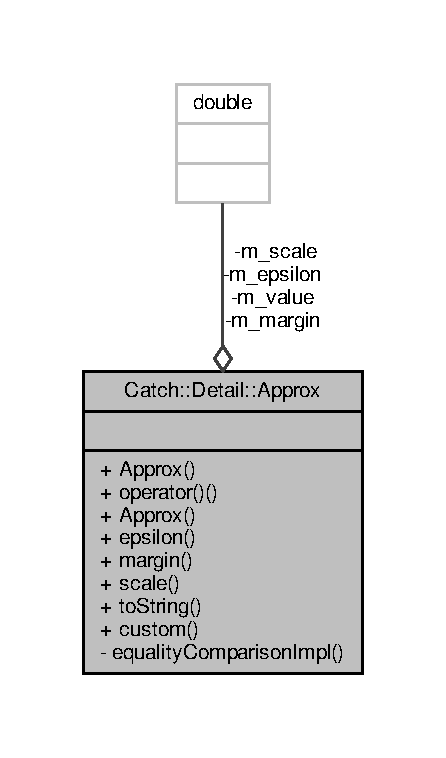
\includegraphics[width=214pt]{class_catch_1_1_detail_1_1_approx__coll__graph}
\end{center}
\end{figure}
\subsection*{Public Member Functions}
\begin{DoxyCompactItemize}
\item 
\hyperlink{class_catch_1_1_detail_1_1_approx_a1a8618ea8db08c66bd3d9fe8f74b957a}{Approx} (double value)
\item 
{\footnotesize template$<$typename T , typename  = typename std\-::enable\-\_\-if$<$std\-::is\-\_\-constructible$<$double, T$>$\-::value$>$\-::type$>$ }\\\hyperlink{class_catch_1_1_detail_1_1_approx}{Approx} \hyperlink{class_catch_1_1_detail_1_1_approx_ad8b2757f4804f9a1d3fa674efb98c20e}{operator()} (T const \&value)
\item 
{\footnotesize template$<$typename T , typename  = typename std\-::enable\-\_\-if$<$std\-::is\-\_\-constructible$<$double, T$>$\-::value$>$\-::type$>$ }\\\hyperlink{class_catch_1_1_detail_1_1_approx_ab14b979fa8a37f21d037157fabed4072}{Approx} (T const \&value)
\item 
{\footnotesize template$<$typename T , typename  = typename std\-::enable\-\_\-if$<$std\-::is\-\_\-constructible$<$double, T$>$\-::value$>$\-::type$>$ }\\\hyperlink{class_catch_1_1_detail_1_1_approx}{Approx} \& \hyperlink{class_catch_1_1_detail_1_1_approx_acd26adba86a066b9f40dad467f23bc85}{epsilon} (T const \&new\-Epsilon)
\item 
{\footnotesize template$<$typename T , typename  = typename std\-::enable\-\_\-if$<$std\-::is\-\_\-constructible$<$double, T$>$\-::value$>$\-::type$>$ }\\\hyperlink{class_catch_1_1_detail_1_1_approx}{Approx} \& \hyperlink{class_catch_1_1_detail_1_1_approx_a6467dc18791e1a1f4c15c4fb63cf5051}{margin} (T const \&new\-Margin)
\item 
{\footnotesize template$<$typename T , typename  = typename std\-::enable\-\_\-if$<$std\-::is\-\_\-constructible$<$double, T$>$\-::value$>$\-::type$>$ }\\\hyperlink{class_catch_1_1_detail_1_1_approx}{Approx} \& \hyperlink{class_catch_1_1_detail_1_1_approx_a8f4d2def2920a3840d3271f6d9c5ede2}{scale} (T const \&new\-Scale)
\item 
std\-::string \hyperlink{class_catch_1_1_detail_1_1_approx_adeb74b73506b3f6b2ba72aea15168fbe}{to\-String} () const 
\end{DoxyCompactItemize}
\subsection*{Static Public Member Functions}
\begin{DoxyCompactItemize}
\item 
static \hyperlink{class_catch_1_1_detail_1_1_approx}{Approx} \hyperlink{class_catch_1_1_detail_1_1_approx_aaf86dc0ee92272ac2d9839197a07951d}{custom} ()
\end{DoxyCompactItemize}
\subsection*{Private Member Functions}
\begin{DoxyCompactItemize}
\item 
bool \hyperlink{class_catch_1_1_detail_1_1_approx_a1ef0f66549a40d1b096aeb4ce685bf9a}{equality\-Comparison\-Impl} (double other) const 
\end{DoxyCompactItemize}
\subsection*{Private Attributes}
\begin{DoxyCompactItemize}
\item 
double \hyperlink{class_catch_1_1_detail_1_1_approx_af17c8e869ae7a55d14b99eb18e178114}{m\-\_\-epsilon}
\item 
double \hyperlink{class_catch_1_1_detail_1_1_approx_a4262a7e821eec507b424c335121ea0d8}{m\-\_\-margin}
\item 
double \hyperlink{class_catch_1_1_detail_1_1_approx_a65e9bdab9113ff3300b45f0a4e048dd7}{m\-\_\-scale}
\item 
double \hyperlink{class_catch_1_1_detail_1_1_approx_af7aeef703bd591f5ec85407b1dac053c}{m\-\_\-value}
\end{DoxyCompactItemize}
\subsection*{Friends}
\begin{DoxyCompactItemize}
\item 
{\footnotesize template$<$typename T , typename  = typename std\-::enable\-\_\-if$<$std\-::is\-\_\-constructible$<$double, T$>$\-::value$>$\-::type$>$ }\\bool \hyperlink{class_catch_1_1_detail_1_1_approx_ab38782a37d09b527ca5e126dbf433dda}{operator==} (const T \&lhs, \hyperlink{class_catch_1_1_detail_1_1_approx}{Approx} const \&rhs)
\item 
{\footnotesize template$<$typename T , typename  = typename std\-::enable\-\_\-if$<$std\-::is\-\_\-constructible$<$double, T$>$\-::value$>$\-::type$>$ }\\bool \hyperlink{class_catch_1_1_detail_1_1_approx_a0e5ef1957d4c38d7857005909c613743}{operator==} (\hyperlink{class_catch_1_1_detail_1_1_approx}{Approx} const \&lhs, const T \&rhs)
\item 
{\footnotesize template$<$typename T , typename  = typename std\-::enable\-\_\-if$<$std\-::is\-\_\-constructible$<$double, T$>$\-::value$>$\-::type$>$ }\\bool \hyperlink{class_catch_1_1_detail_1_1_approx_a29696f14ebd51887c8c88e771d12ef54}{operator!=} (T const \&lhs, \hyperlink{class_catch_1_1_detail_1_1_approx}{Approx} const \&rhs)
\item 
{\footnotesize template$<$typename T , typename  = typename std\-::enable\-\_\-if$<$std\-::is\-\_\-constructible$<$double, T$>$\-::value$>$\-::type$>$ }\\bool \hyperlink{class_catch_1_1_detail_1_1_approx_a31d62e3c35abb86cf25e02601966ca5d}{operator!=} (\hyperlink{class_catch_1_1_detail_1_1_approx}{Approx} const \&lhs, T const \&rhs)
\item 
{\footnotesize template$<$typename T , typename  = typename std\-::enable\-\_\-if$<$std\-::is\-\_\-constructible$<$double, T$>$\-::value$>$\-::type$>$ }\\bool \hyperlink{class_catch_1_1_detail_1_1_approx_a0369de03e81bc2ceaf6c9d830476bd49}{operator$<$=} (T const \&lhs, \hyperlink{class_catch_1_1_detail_1_1_approx}{Approx} const \&rhs)
\item 
{\footnotesize template$<$typename T , typename  = typename std\-::enable\-\_\-if$<$std\-::is\-\_\-constructible$<$double, T$>$\-::value$>$\-::type$>$ }\\bool \hyperlink{class_catch_1_1_detail_1_1_approx_a6040b908588745570847d7ae8483b091}{operator$<$=} (\hyperlink{class_catch_1_1_detail_1_1_approx}{Approx} const \&lhs, T const \&rhs)
\item 
{\footnotesize template$<$typename T , typename  = typename std\-::enable\-\_\-if$<$std\-::is\-\_\-constructible$<$double, T$>$\-::value$>$\-::type$>$ }\\bool \hyperlink{class_catch_1_1_detail_1_1_approx_affd27efc62be386daeecb7a09e828d44}{operator$>$=} (T const \&lhs, \hyperlink{class_catch_1_1_detail_1_1_approx}{Approx} const \&rhs)
\item 
{\footnotesize template$<$typename T , typename  = typename std\-::enable\-\_\-if$<$std\-::is\-\_\-constructible$<$double, T$>$\-::value$>$\-::type$>$ }\\bool \hyperlink{class_catch_1_1_detail_1_1_approx_a5899b8a36725406701e2ebded2971ee6}{operator$>$=} (\hyperlink{class_catch_1_1_detail_1_1_approx}{Approx} const \&lhs, T const \&rhs)
\end{DoxyCompactItemize}


\subsection{Constructor \& Destructor Documentation}
\hypertarget{class_catch_1_1_detail_1_1_approx_a1a8618ea8db08c66bd3d9fe8f74b957a}{\index{Catch\-::\-Detail\-::\-Approx@{Catch\-::\-Detail\-::\-Approx}!Approx@{Approx}}
\index{Approx@{Approx}!Catch::Detail::Approx@{Catch\-::\-Detail\-::\-Approx}}
\subsubsection[{Approx}]{\setlength{\rightskip}{0pt plus 5cm}Catch\-::\-Detail\-::\-Approx\-::\-Approx (
\begin{DoxyParamCaption}
\item[{double}]{value}
\end{DoxyParamCaption}
)\hspace{0.3cm}{\ttfamily [explicit]}}}\label{class_catch_1_1_detail_1_1_approx_a1a8618ea8db08c66bd3d9fe8f74b957a}
\hypertarget{class_catch_1_1_detail_1_1_approx_ab14b979fa8a37f21d037157fabed4072}{\index{Catch\-::\-Detail\-::\-Approx@{Catch\-::\-Detail\-::\-Approx}!Approx@{Approx}}
\index{Approx@{Approx}!Catch::Detail::Approx@{Catch\-::\-Detail\-::\-Approx}}
\subsubsection[{Approx}]{\setlength{\rightskip}{0pt plus 5cm}template$<$typename T , typename  = typename std\-::enable\-\_\-if$<$std\-::is\-\_\-constructible$<$double, T$>$\-::value$>$\-::type$>$ Catch\-::\-Detail\-::\-Approx\-::\-Approx (
\begin{DoxyParamCaption}
\item[{T const \&}]{value}
\end{DoxyParamCaption}
)\hspace{0.3cm}{\ttfamily [inline]}, {\ttfamily [explicit]}}}\label{class_catch_1_1_detail_1_1_approx_ab14b979fa8a37f21d037157fabed4072}

\begin{DoxyCode}
2090                                             : \hyperlink{class_catch_1_1_detail_1_1_approx_a1a8618ea8db08c66bd3d9fe8f74b957a}{Approx}(static\_cast<double>(value))
2091             \{\}
\end{DoxyCode}


\subsection{Member Function Documentation}
\hypertarget{class_catch_1_1_detail_1_1_approx_aaf86dc0ee92272ac2d9839197a07951d}{\index{Catch\-::\-Detail\-::\-Approx@{Catch\-::\-Detail\-::\-Approx}!custom@{custom}}
\index{custom@{custom}!Catch::Detail::Approx@{Catch\-::\-Detail\-::\-Approx}}
\subsubsection[{custom}]{\setlength{\rightskip}{0pt plus 5cm}static {\bf Approx} Catch\-::\-Detail\-::\-Approx\-::custom (
\begin{DoxyParamCaption}
{}
\end{DoxyParamCaption}
)\hspace{0.3cm}{\ttfamily [static]}}}\label{class_catch_1_1_detail_1_1_approx_aaf86dc0ee92272ac2d9839197a07951d}
\hypertarget{class_catch_1_1_detail_1_1_approx_acd26adba86a066b9f40dad467f23bc85}{\index{Catch\-::\-Detail\-::\-Approx@{Catch\-::\-Detail\-::\-Approx}!epsilon@{epsilon}}
\index{epsilon@{epsilon}!Catch::Detail::Approx@{Catch\-::\-Detail\-::\-Approx}}
\subsubsection[{epsilon}]{\setlength{\rightskip}{0pt plus 5cm}template$<$typename T , typename  = typename std\-::enable\-\_\-if$<$std\-::is\-\_\-constructible$<$double, T$>$\-::value$>$\-::type$>$ {\bf Approx}\& Catch\-::\-Detail\-::\-Approx\-::epsilon (
\begin{DoxyParamCaption}
\item[{T const \&}]{new\-Epsilon}
\end{DoxyParamCaption}
)\hspace{0.3cm}{\ttfamily [inline]}}}\label{class_catch_1_1_detail_1_1_approx_acd26adba86a066b9f40dad467f23bc85}


References Catch\-::\-Detail\-::stringify().



Referenced by operator()().


\begin{DoxyCode}
2135                                                  \{
2136                 \textcolor{keywordtype}{double} epsilonAsDouble = \textcolor{keyword}{static\_cast<}\textcolor{keywordtype}{double}\textcolor{keyword}{>}(newEpsilon);
2137                 \textcolor{keywordflow}{if} (epsilonAsDouble < 0 || epsilonAsDouble > 1.0) \{
2138                     \textcolor{keywordflow}{throw} std::domain\_error
2139                     (\textcolor{stringliteral}{"Invalid Approx::epsilon: "} +
2140                         \hyperlink{namespace_catch_1_1_detail_af0ad48344ffd3f92f3568465248a9880}{Catch::Detail::stringify}(epsilonAsDouble) +
2141                         \textcolor{stringliteral}{", Approx::epsilon has to be between 0 and 1"});
2142                 \}
2143                 \hyperlink{class_catch_1_1_detail_1_1_approx_af17c8e869ae7a55d14b99eb18e178114}{m\_epsilon} = epsilonAsDouble;
2144                 \textcolor{keywordflow}{return} *\textcolor{keyword}{this};
2145             \}
\end{DoxyCode}
\hypertarget{class_catch_1_1_detail_1_1_approx_a1ef0f66549a40d1b096aeb4ce685bf9a}{\index{Catch\-::\-Detail\-::\-Approx@{Catch\-::\-Detail\-::\-Approx}!equality\-Comparison\-Impl@{equality\-Comparison\-Impl}}
\index{equality\-Comparison\-Impl@{equality\-Comparison\-Impl}!Catch::Detail::Approx@{Catch\-::\-Detail\-::\-Approx}}
\subsubsection[{equality\-Comparison\-Impl}]{\setlength{\rightskip}{0pt plus 5cm}bool Catch\-::\-Detail\-::\-Approx\-::equality\-Comparison\-Impl (
\begin{DoxyParamCaption}
\item[{double}]{other}
\end{DoxyParamCaption}
) const\hspace{0.3cm}{\ttfamily [private]}}}\label{class_catch_1_1_detail_1_1_approx_a1ef0f66549a40d1b096aeb4ce685bf9a}
\hypertarget{class_catch_1_1_detail_1_1_approx_a6467dc18791e1a1f4c15c4fb63cf5051}{\index{Catch\-::\-Detail\-::\-Approx@{Catch\-::\-Detail\-::\-Approx}!margin@{margin}}
\index{margin@{margin}!Catch::Detail::Approx@{Catch\-::\-Detail\-::\-Approx}}
\subsubsection[{margin}]{\setlength{\rightskip}{0pt plus 5cm}template$<$typename T , typename  = typename std\-::enable\-\_\-if$<$std\-::is\-\_\-constructible$<$double, T$>$\-::value$>$\-::type$>$ {\bf Approx}\& Catch\-::\-Detail\-::\-Approx\-::margin (
\begin{DoxyParamCaption}
\item[{T const \&}]{new\-Margin}
\end{DoxyParamCaption}
)\hspace{0.3cm}{\ttfamily [inline]}}}\label{class_catch_1_1_detail_1_1_approx_a6467dc18791e1a1f4c15c4fb63cf5051}


References Catch\-::\-Detail\-::stringify().



Referenced by operator()().


\begin{DoxyCode}
2148                                                \{
2149                 \textcolor{keywordtype}{double} marginAsDouble = \textcolor{keyword}{static\_cast<}\textcolor{keywordtype}{double}\textcolor{keyword}{>}(newMargin);
2150                 \textcolor{keywordflow}{if} (marginAsDouble < 0) \{
2151                     \textcolor{keywordflow}{throw} std::domain\_error
2152                     (\textcolor{stringliteral}{"Invalid Approx::margin: "} +
2153                         \hyperlink{namespace_catch_1_1_detail_af0ad48344ffd3f92f3568465248a9880}{Catch::Detail::stringify}(marginAsDouble) +
2154                         \textcolor{stringliteral}{", Approx::Margin has to be non-negative."});
2155 
2156                 \}
2157                 \hyperlink{class_catch_1_1_detail_1_1_approx_a4262a7e821eec507b424c335121ea0d8}{m\_margin} = marginAsDouble;
2158                 \textcolor{keywordflow}{return} *\textcolor{keyword}{this};
2159             \}
\end{DoxyCode}
\hypertarget{class_catch_1_1_detail_1_1_approx_ad8b2757f4804f9a1d3fa674efb98c20e}{\index{Catch\-::\-Detail\-::\-Approx@{Catch\-::\-Detail\-::\-Approx}!operator()@{operator()}}
\index{operator()@{operator()}!Catch::Detail::Approx@{Catch\-::\-Detail\-::\-Approx}}
\subsubsection[{operator()}]{\setlength{\rightskip}{0pt plus 5cm}template$<$typename T , typename  = typename std\-::enable\-\_\-if$<$std\-::is\-\_\-constructible$<$double, T$>$\-::value$>$\-::type$>$ {\bf Approx} Catch\-::\-Detail\-::\-Approx\-::operator() (
\begin{DoxyParamCaption}
\item[{T const \&}]{value}
\end{DoxyParamCaption}
)\hspace{0.3cm}{\ttfamily [inline]}}}\label{class_catch_1_1_detail_1_1_approx_ad8b2757f4804f9a1d3fa674efb98c20e}


References epsilon(), margin(), and scale().


\begin{DoxyCode}
2081                                               \{
2082                 \hyperlink{class_catch_1_1_detail_1_1_approx}{Approx} approx(static\_cast<double>(value));
2083                 approx.epsilon(\hyperlink{class_catch_1_1_detail_1_1_approx_af17c8e869ae7a55d14b99eb18e178114}{m\_epsilon});
2084                 approx.margin(\hyperlink{class_catch_1_1_detail_1_1_approx_a4262a7e821eec507b424c335121ea0d8}{m\_margin});
2085                 approx.scale(\hyperlink{class_catch_1_1_detail_1_1_approx_a65e9bdab9113ff3300b45f0a4e048dd7}{m\_scale});
2086                 \textcolor{keywordflow}{return} approx;
2087             \}
\end{DoxyCode}
\hypertarget{class_catch_1_1_detail_1_1_approx_a8f4d2def2920a3840d3271f6d9c5ede2}{\index{Catch\-::\-Detail\-::\-Approx@{Catch\-::\-Detail\-::\-Approx}!scale@{scale}}
\index{scale@{scale}!Catch::Detail::Approx@{Catch\-::\-Detail\-::\-Approx}}
\subsubsection[{scale}]{\setlength{\rightskip}{0pt plus 5cm}template$<$typename T , typename  = typename std\-::enable\-\_\-if$<$std\-::is\-\_\-constructible$<$double, T$>$\-::value$>$\-::type$>$ {\bf Approx}\& Catch\-::\-Detail\-::\-Approx\-::scale (
\begin{DoxyParamCaption}
\item[{T const \&}]{new\-Scale}
\end{DoxyParamCaption}
)\hspace{0.3cm}{\ttfamily [inline]}}}\label{class_catch_1_1_detail_1_1_approx_a8f4d2def2920a3840d3271f6d9c5ede2}


Referenced by operator()().


\begin{DoxyCode}
2162                                              \{
2163                 \hyperlink{class_catch_1_1_detail_1_1_approx_a65e9bdab9113ff3300b45f0a4e048dd7}{m\_scale} = \textcolor{keyword}{static\_cast<}\textcolor{keywordtype}{double}\textcolor{keyword}{>}(newScale);
2164                 \textcolor{keywordflow}{return} *\textcolor{keyword}{this};
2165             \}
\end{DoxyCode}
\hypertarget{class_catch_1_1_detail_1_1_approx_adeb74b73506b3f6b2ba72aea15168fbe}{\index{Catch\-::\-Detail\-::\-Approx@{Catch\-::\-Detail\-::\-Approx}!to\-String@{to\-String}}
\index{to\-String@{to\-String}!Catch::Detail::Approx@{Catch\-::\-Detail\-::\-Approx}}
\subsubsection[{to\-String}]{\setlength{\rightskip}{0pt plus 5cm}std\-::string Catch\-::\-Detail\-::\-Approx\-::to\-String (
\begin{DoxyParamCaption}
{}
\end{DoxyParamCaption}
) const}}\label{class_catch_1_1_detail_1_1_approx_adeb74b73506b3f6b2ba72aea15168fbe}


\subsection{Friends And Related Function Documentation}
\hypertarget{class_catch_1_1_detail_1_1_approx_a29696f14ebd51887c8c88e771d12ef54}{\index{Catch\-::\-Detail\-::\-Approx@{Catch\-::\-Detail\-::\-Approx}!operator!=@{operator!=}}
\index{operator!=@{operator!=}!Catch::Detail::Approx@{Catch\-::\-Detail\-::\-Approx}}
\subsubsection[{operator!=}]{\setlength{\rightskip}{0pt plus 5cm}template$<$typename T , typename  = typename std\-::enable\-\_\-if$<$std\-::is\-\_\-constructible$<$double, T$>$\-::value$>$\-::type$>$ bool operator!= (
\begin{DoxyParamCaption}
\item[{T const \&}]{lhs, }
\item[{{\bf Approx} const \&}]{rhs}
\end{DoxyParamCaption}
)\hspace{0.3cm}{\ttfamily [friend]}}}\label{class_catch_1_1_detail_1_1_approx_a29696f14ebd51887c8c88e771d12ef54}

\begin{DoxyCode}
2105                                                                       \{
2106                 \textcolor{keywordflow}{return} !\hyperlink{class_catch_1_1_detail_1_1_approx_ab38782a37d09b527ca5e126dbf433dda}{operator==}(lhs, rhs);
2107             \}
\end{DoxyCode}
\hypertarget{class_catch_1_1_detail_1_1_approx_a31d62e3c35abb86cf25e02601966ca5d}{\index{Catch\-::\-Detail\-::\-Approx@{Catch\-::\-Detail\-::\-Approx}!operator!=@{operator!=}}
\index{operator!=@{operator!=}!Catch::Detail::Approx@{Catch\-::\-Detail\-::\-Approx}}
\subsubsection[{operator!=}]{\setlength{\rightskip}{0pt plus 5cm}template$<$typename T , typename  = typename std\-::enable\-\_\-if$<$std\-::is\-\_\-constructible$<$double, T$>$\-::value$>$\-::type$>$ bool operator!= (
\begin{DoxyParamCaption}
\item[{{\bf Approx} const \&}]{lhs, }
\item[{T const \&}]{rhs}
\end{DoxyParamCaption}
)\hspace{0.3cm}{\ttfamily [friend]}}}\label{class_catch_1_1_detail_1_1_approx_a31d62e3c35abb86cf25e02601966ca5d}

\begin{DoxyCode}
2110                                                                       \{
2111                 \textcolor{keywordflow}{return} !\hyperlink{class_catch_1_1_detail_1_1_approx_ab38782a37d09b527ca5e126dbf433dda}{operator==}(rhs, lhs);
2112             \}
\end{DoxyCode}
\hypertarget{class_catch_1_1_detail_1_1_approx_a0369de03e81bc2ceaf6c9d830476bd49}{\index{Catch\-::\-Detail\-::\-Approx@{Catch\-::\-Detail\-::\-Approx}!operator$<$=@{operator$<$=}}
\index{operator$<$=@{operator$<$=}!Catch::Detail::Approx@{Catch\-::\-Detail\-::\-Approx}}
\subsubsection[{operator$<$=}]{\setlength{\rightskip}{0pt plus 5cm}template$<$typename T , typename  = typename std\-::enable\-\_\-if$<$std\-::is\-\_\-constructible$<$double, T$>$\-::value$>$\-::type$>$ bool operator$<$= (
\begin{DoxyParamCaption}
\item[{T const \&}]{lhs, }
\item[{{\bf Approx} const \&}]{rhs}
\end{DoxyParamCaption}
)\hspace{0.3cm}{\ttfamily [friend]}}}\label{class_catch_1_1_detail_1_1_approx_a0369de03e81bc2ceaf6c9d830476bd49}

\begin{DoxyCode}
2115                                                                       \{
2116                 \textcolor{keywordflow}{return} \textcolor{keyword}{static\_cast<}\textcolor{keywordtype}{double}\textcolor{keyword}{>}(lhs) < rhs.m\_value || lhs == rhs;
2117             \}
\end{DoxyCode}
\hypertarget{class_catch_1_1_detail_1_1_approx_a6040b908588745570847d7ae8483b091}{\index{Catch\-::\-Detail\-::\-Approx@{Catch\-::\-Detail\-::\-Approx}!operator$<$=@{operator$<$=}}
\index{operator$<$=@{operator$<$=}!Catch::Detail::Approx@{Catch\-::\-Detail\-::\-Approx}}
\subsubsection[{operator$<$=}]{\setlength{\rightskip}{0pt plus 5cm}template$<$typename T , typename  = typename std\-::enable\-\_\-if$<$std\-::is\-\_\-constructible$<$double, T$>$\-::value$>$\-::type$>$ bool operator$<$= (
\begin{DoxyParamCaption}
\item[{{\bf Approx} const \&}]{lhs, }
\item[{T const \&}]{rhs}
\end{DoxyParamCaption}
)\hspace{0.3cm}{\ttfamily [friend]}}}\label{class_catch_1_1_detail_1_1_approx_a6040b908588745570847d7ae8483b091}

\begin{DoxyCode}
2120                                                                       \{
2121                 \textcolor{keywordflow}{return} lhs.m\_value < \textcolor{keyword}{static\_cast<}\textcolor{keywordtype}{double}\textcolor{keyword}{>}(rhs) || lhs == rhs;
2122             \}
\end{DoxyCode}
\hypertarget{class_catch_1_1_detail_1_1_approx_ab38782a37d09b527ca5e126dbf433dda}{\index{Catch\-::\-Detail\-::\-Approx@{Catch\-::\-Detail\-::\-Approx}!operator==@{operator==}}
\index{operator==@{operator==}!Catch::Detail::Approx@{Catch\-::\-Detail\-::\-Approx}}
\subsubsection[{operator==}]{\setlength{\rightskip}{0pt plus 5cm}template$<$typename T , typename  = typename std\-::enable\-\_\-if$<$std\-::is\-\_\-constructible$<$double, T$>$\-::value$>$\-::type$>$ bool operator== (
\begin{DoxyParamCaption}
\item[{const T \&}]{lhs, }
\item[{{\bf Approx} const \&}]{rhs}
\end{DoxyParamCaption}
)\hspace{0.3cm}{\ttfamily [friend]}}}\label{class_catch_1_1_detail_1_1_approx_ab38782a37d09b527ca5e126dbf433dda}

\begin{DoxyCode}
2094                                                                       \{
2095                 \textcolor{keyword}{auto} lhs\_v = \textcolor{keyword}{static\_cast<}\textcolor{keywordtype}{double}\textcolor{keyword}{>}(lhs);
2096                 \textcolor{keywordflow}{return} rhs.equalityComparisonImpl(lhs\_v);
2097             \}
\end{DoxyCode}
\hypertarget{class_catch_1_1_detail_1_1_approx_a0e5ef1957d4c38d7857005909c613743}{\index{Catch\-::\-Detail\-::\-Approx@{Catch\-::\-Detail\-::\-Approx}!operator==@{operator==}}
\index{operator==@{operator==}!Catch::Detail::Approx@{Catch\-::\-Detail\-::\-Approx}}
\subsubsection[{operator==}]{\setlength{\rightskip}{0pt plus 5cm}template$<$typename T , typename  = typename std\-::enable\-\_\-if$<$std\-::is\-\_\-constructible$<$double, T$>$\-::value$>$\-::type$>$ bool operator== (
\begin{DoxyParamCaption}
\item[{{\bf Approx} const \&}]{lhs, }
\item[{const T \&}]{rhs}
\end{DoxyParamCaption}
)\hspace{0.3cm}{\ttfamily [friend]}}}\label{class_catch_1_1_detail_1_1_approx_a0e5ef1957d4c38d7857005909c613743}

\begin{DoxyCode}
2100                                                                       \{
2101                 \textcolor{keywordflow}{return} \hyperlink{class_catch_1_1_detail_1_1_approx_ab38782a37d09b527ca5e126dbf433dda}{operator==}(rhs, lhs);
2102             \}
\end{DoxyCode}
\hypertarget{class_catch_1_1_detail_1_1_approx_affd27efc62be386daeecb7a09e828d44}{\index{Catch\-::\-Detail\-::\-Approx@{Catch\-::\-Detail\-::\-Approx}!operator$>$=@{operator$>$=}}
\index{operator$>$=@{operator$>$=}!Catch::Detail::Approx@{Catch\-::\-Detail\-::\-Approx}}
\subsubsection[{operator$>$=}]{\setlength{\rightskip}{0pt plus 5cm}template$<$typename T , typename  = typename std\-::enable\-\_\-if$<$std\-::is\-\_\-constructible$<$double, T$>$\-::value$>$\-::type$>$ bool operator$>$= (
\begin{DoxyParamCaption}
\item[{T const \&}]{lhs, }
\item[{{\bf Approx} const \&}]{rhs}
\end{DoxyParamCaption}
)\hspace{0.3cm}{\ttfamily [friend]}}}\label{class_catch_1_1_detail_1_1_approx_affd27efc62be386daeecb7a09e828d44}

\begin{DoxyCode}
2125                                                                       \{
2126                 \textcolor{keywordflow}{return} \textcolor{keyword}{static\_cast<}\textcolor{keywordtype}{double}\textcolor{keyword}{>}(lhs) > rhs.m\_value || lhs == rhs;
2127             \}
\end{DoxyCode}
\hypertarget{class_catch_1_1_detail_1_1_approx_a5899b8a36725406701e2ebded2971ee6}{\index{Catch\-::\-Detail\-::\-Approx@{Catch\-::\-Detail\-::\-Approx}!operator$>$=@{operator$>$=}}
\index{operator$>$=@{operator$>$=}!Catch::Detail::Approx@{Catch\-::\-Detail\-::\-Approx}}
\subsubsection[{operator$>$=}]{\setlength{\rightskip}{0pt plus 5cm}template$<$typename T , typename  = typename std\-::enable\-\_\-if$<$std\-::is\-\_\-constructible$<$double, T$>$\-::value$>$\-::type$>$ bool operator$>$= (
\begin{DoxyParamCaption}
\item[{{\bf Approx} const \&}]{lhs, }
\item[{T const \&}]{rhs}
\end{DoxyParamCaption}
)\hspace{0.3cm}{\ttfamily [friend]}}}\label{class_catch_1_1_detail_1_1_approx_a5899b8a36725406701e2ebded2971ee6}

\begin{DoxyCode}
2130                                                                       \{
2131                 \textcolor{keywordflow}{return} lhs.m\_value > \textcolor{keyword}{static\_cast<}\textcolor{keywordtype}{double}\textcolor{keyword}{>}(rhs) || lhs == rhs;
2132             \}
\end{DoxyCode}


\subsection{Member Data Documentation}
\hypertarget{class_catch_1_1_detail_1_1_approx_af17c8e869ae7a55d14b99eb18e178114}{\index{Catch\-::\-Detail\-::\-Approx@{Catch\-::\-Detail\-::\-Approx}!m\-\_\-epsilon@{m\-\_\-epsilon}}
\index{m\-\_\-epsilon@{m\-\_\-epsilon}!Catch::Detail::Approx@{Catch\-::\-Detail\-::\-Approx}}
\subsubsection[{m\-\_\-epsilon}]{\setlength{\rightskip}{0pt plus 5cm}double Catch\-::\-Detail\-::\-Approx\-::m\-\_\-epsilon\hspace{0.3cm}{\ttfamily [private]}}}\label{class_catch_1_1_detail_1_1_approx_af17c8e869ae7a55d14b99eb18e178114}
\hypertarget{class_catch_1_1_detail_1_1_approx_a4262a7e821eec507b424c335121ea0d8}{\index{Catch\-::\-Detail\-::\-Approx@{Catch\-::\-Detail\-::\-Approx}!m\-\_\-margin@{m\-\_\-margin}}
\index{m\-\_\-margin@{m\-\_\-margin}!Catch::Detail::Approx@{Catch\-::\-Detail\-::\-Approx}}
\subsubsection[{m\-\_\-margin}]{\setlength{\rightskip}{0pt plus 5cm}double Catch\-::\-Detail\-::\-Approx\-::m\-\_\-margin\hspace{0.3cm}{\ttfamily [private]}}}\label{class_catch_1_1_detail_1_1_approx_a4262a7e821eec507b424c335121ea0d8}
\hypertarget{class_catch_1_1_detail_1_1_approx_a65e9bdab9113ff3300b45f0a4e048dd7}{\index{Catch\-::\-Detail\-::\-Approx@{Catch\-::\-Detail\-::\-Approx}!m\-\_\-scale@{m\-\_\-scale}}
\index{m\-\_\-scale@{m\-\_\-scale}!Catch::Detail::Approx@{Catch\-::\-Detail\-::\-Approx}}
\subsubsection[{m\-\_\-scale}]{\setlength{\rightskip}{0pt plus 5cm}double Catch\-::\-Detail\-::\-Approx\-::m\-\_\-scale\hspace{0.3cm}{\ttfamily [private]}}}\label{class_catch_1_1_detail_1_1_approx_a65e9bdab9113ff3300b45f0a4e048dd7}
\hypertarget{class_catch_1_1_detail_1_1_approx_af7aeef703bd591f5ec85407b1dac053c}{\index{Catch\-::\-Detail\-::\-Approx@{Catch\-::\-Detail\-::\-Approx}!m\-\_\-value@{m\-\_\-value}}
\index{m\-\_\-value@{m\-\_\-value}!Catch::Detail::Approx@{Catch\-::\-Detail\-::\-Approx}}
\subsubsection[{m\-\_\-value}]{\setlength{\rightskip}{0pt plus 5cm}double Catch\-::\-Detail\-::\-Approx\-::m\-\_\-value\hspace{0.3cm}{\ttfamily [private]}}}\label{class_catch_1_1_detail_1_1_approx_af7aeef703bd591f5ec85407b1dac053c}


The documentation for this class was generated from the following file\-:\begin{DoxyCompactItemize}
\item 
\hyperlink{catch_8hpp}{catch.\-hpp}\end{DoxyCompactItemize}

\hypertarget{class_catch_1_1_assertion_handler}{\section{Catch\-:\-:Assertion\-Handler Class Reference}
\label{class_catch_1_1_assertion_handler}\index{Catch\-::\-Assertion\-Handler@{Catch\-::\-Assertion\-Handler}}
}


{\ttfamily \#include $<$catch.\-hpp$>$}



Collaboration diagram for Catch\-:\-:Assertion\-Handler\-:
\nopagebreak
\begin{figure}[H]
\begin{center}
\leavevmode
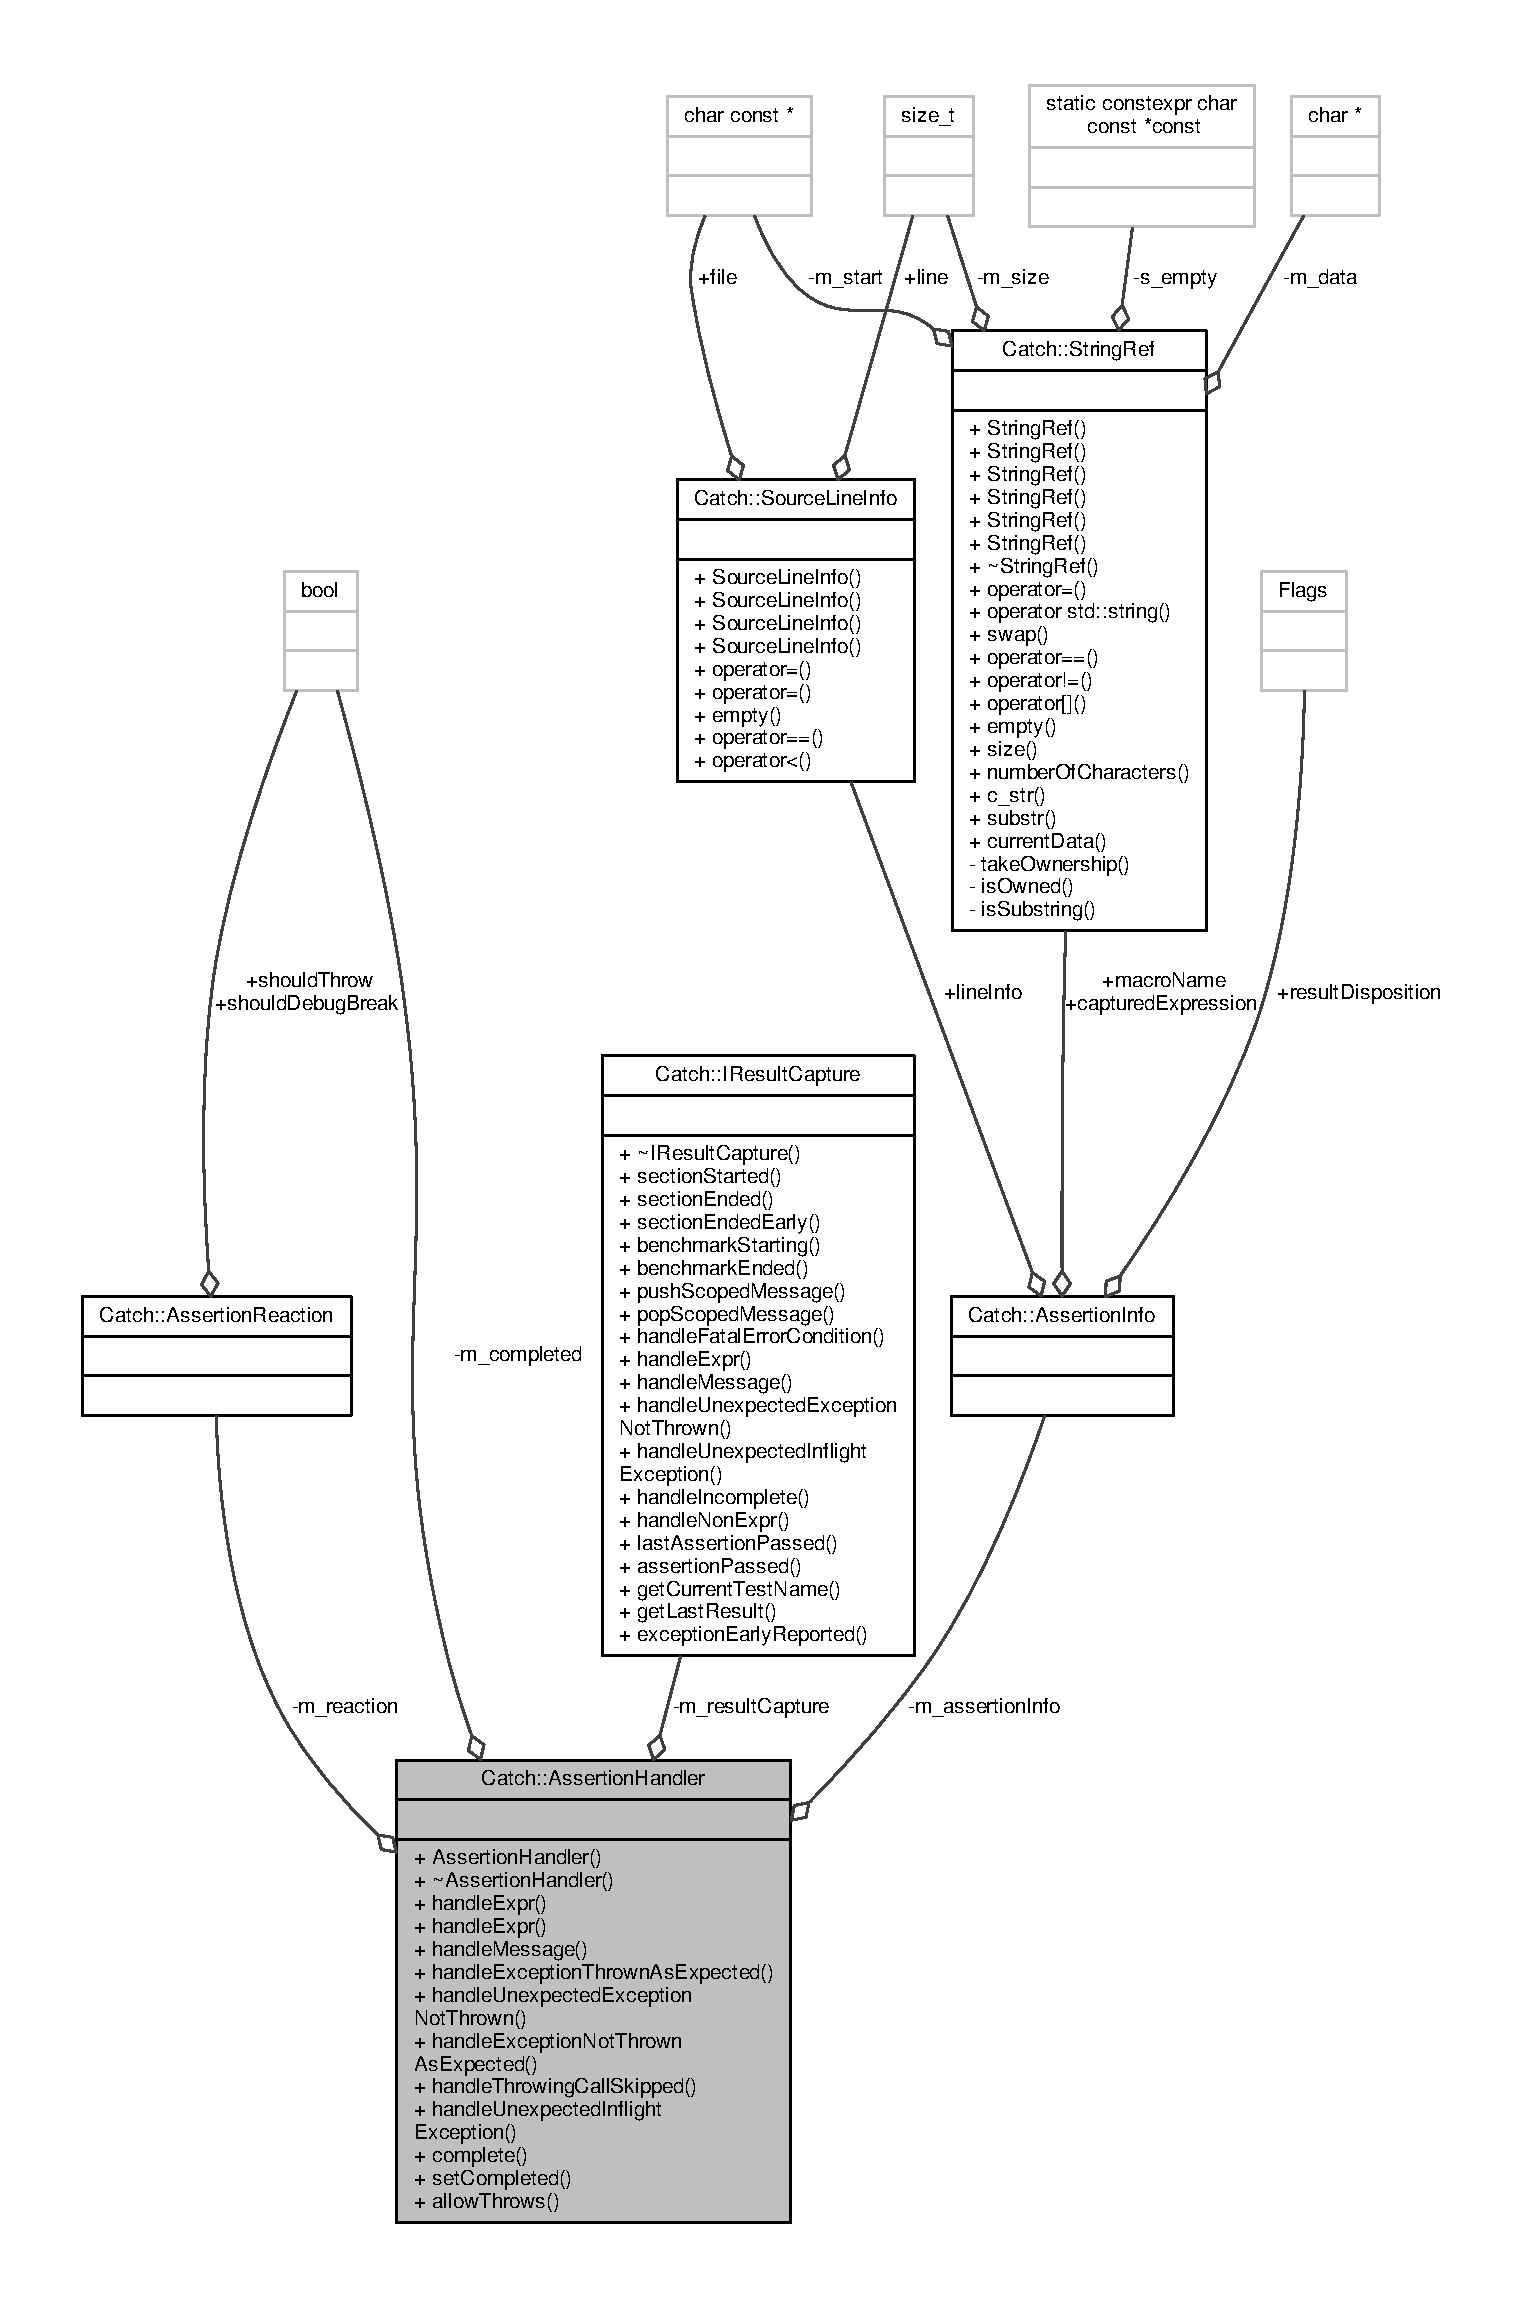
\includegraphics[width=350pt]{class_catch_1_1_assertion_handler__coll__graph}
\end{center}
\end{figure}
\subsection*{Public Member Functions}
\begin{DoxyCompactItemize}
\item 
\hyperlink{class_catch_1_1_assertion_handler_a74627e1e399b026e9acbaf95ea673643}{Assertion\-Handler} (\hyperlink{class_catch_1_1_string_ref}{String\-Ref} macro\-Name, \hyperlink{struct_catch_1_1_source_line_info}{Source\-Line\-Info} const \&line\-Info, \hyperlink{class_catch_1_1_string_ref}{String\-Ref} captured\-Expression, \hyperlink{struct_catch_1_1_result_disposition_a3396cad6e2259af326b3aae93e23e9d8}{Result\-Disposition\-::\-Flags} result\-Disposition)
\item 
\hyperlink{class_catch_1_1_assertion_handler_a1e839d810f6ac0fa6d127fe8350175ed}{$\sim$\-Assertion\-Handler} ()
\item 
{\footnotesize template$<$typename T $>$ }\\void \hyperlink{class_catch_1_1_assertion_handler_a2ef387e567bad90ec6e4b5bf5c367388}{handle\-Expr} (\hyperlink{class_catch_1_1_expr_lhs}{Expr\-Lhs}$<$ T $>$ const \&expr)
\item 
void \hyperlink{class_catch_1_1_assertion_handler_afe14d9cf1b1c7f70dae439fbdb51d0c4}{handle\-Expr} (\hyperlink{struct_catch_1_1_i_transient_expression}{I\-Transient\-Expression} const \&expr)
\item 
void \hyperlink{class_catch_1_1_assertion_handler_abdb4c180ed83ec2858b2fb87712c516d}{handle\-Message} (\hyperlink{struct_catch_1_1_result_was_a624e1ee3661fcf6094ceef1f654601ef}{Result\-Was\-::\-Of\-Type} result\-Type, \hyperlink{class_catch_1_1_string_ref}{String\-Ref} const \&message)
\item 
void \hyperlink{class_catch_1_1_assertion_handler_ab6caf765764a4064e90fce829eec201d}{handle\-Exception\-Thrown\-As\-Expected} ()
\item 
void \hyperlink{class_catch_1_1_assertion_handler_a7764d0adb6ed5eeb10964f6abc02fab1}{handle\-Unexpected\-Exception\-Not\-Thrown} ()
\item 
void \hyperlink{class_catch_1_1_assertion_handler_a51e4936e3af43b74690cedae6d2e297a}{handle\-Exception\-Not\-Thrown\-As\-Expected} ()
\item 
void \hyperlink{class_catch_1_1_assertion_handler_a67a194d5518f307c4a16faa03a7f7442}{handle\-Throwing\-Call\-Skipped} ()
\item 
void \hyperlink{class_catch_1_1_assertion_handler_aa2504dad6a91f3645e5f52c932c11270}{handle\-Unexpected\-Inflight\-Exception} ()
\item 
void \hyperlink{class_catch_1_1_assertion_handler_a878a9eb828d8a1863c8dcb6575f6f40e}{complete} ()
\item 
void \hyperlink{class_catch_1_1_assertion_handler_a6756bd5395c0ddd28764a9fb4612d5e4}{set\-Completed} ()
\item 
auto \hyperlink{class_catch_1_1_assertion_handler_a193bb3999494c46457f3059184c6b251}{allow\-Throws} () const -\/$>$ bool
\end{DoxyCompactItemize}
\subsection*{Private Attributes}
\begin{DoxyCompactItemize}
\item 
\hyperlink{struct_catch_1_1_assertion_info}{Assertion\-Info} \hyperlink{class_catch_1_1_assertion_handler_ad171e8724bb771d97949b7270f400303}{m\-\_\-assertion\-Info}
\item 
\hyperlink{struct_catch_1_1_assertion_reaction}{Assertion\-Reaction} \hyperlink{class_catch_1_1_assertion_handler_a8203c08a43a3761b5f400ee6587fad55}{m\-\_\-reaction}
\item 
bool \hyperlink{class_catch_1_1_assertion_handler_a5a756818dff781c155e8eb970d1d4c68}{m\-\_\-completed} = false
\item 
\hyperlink{struct_catch_1_1_i_result_capture}{I\-Result\-Capture} \& \hyperlink{class_catch_1_1_assertion_handler_aea5283ee36124ce5c51dc2a697b22a39}{m\-\_\-result\-Capture}
\end{DoxyCompactItemize}


\subsection{Constructor \& Destructor Documentation}
\hypertarget{class_catch_1_1_assertion_handler_a74627e1e399b026e9acbaf95ea673643}{\index{Catch\-::\-Assertion\-Handler@{Catch\-::\-Assertion\-Handler}!Assertion\-Handler@{Assertion\-Handler}}
\index{Assertion\-Handler@{Assertion\-Handler}!Catch::AssertionHandler@{Catch\-::\-Assertion\-Handler}}
\subsubsection[{Assertion\-Handler}]{\setlength{\rightskip}{0pt plus 5cm}Catch\-::\-Assertion\-Handler\-::\-Assertion\-Handler (
\begin{DoxyParamCaption}
\item[{{\bf String\-Ref}}]{macro\-Name, }
\item[{{\bf Source\-Line\-Info} const \&}]{line\-Info, }
\item[{{\bf String\-Ref}}]{captured\-Expression, }
\item[{{\bf Result\-Disposition\-::\-Flags}}]{result\-Disposition}
\end{DoxyParamCaption}
)}}\label{class_catch_1_1_assertion_handler_a74627e1e399b026e9acbaf95ea673643}
\hypertarget{class_catch_1_1_assertion_handler_a1e839d810f6ac0fa6d127fe8350175ed}{\index{Catch\-::\-Assertion\-Handler@{Catch\-::\-Assertion\-Handler}!$\sim$\-Assertion\-Handler@{$\sim$\-Assertion\-Handler}}
\index{$\sim$\-Assertion\-Handler@{$\sim$\-Assertion\-Handler}!Catch::AssertionHandler@{Catch\-::\-Assertion\-Handler}}
\subsubsection[{$\sim$\-Assertion\-Handler}]{\setlength{\rightskip}{0pt plus 5cm}Catch\-::\-Assertion\-Handler\-::$\sim$\-Assertion\-Handler (
\begin{DoxyParamCaption}
{}
\end{DoxyParamCaption}
)\hspace{0.3cm}{\ttfamily [inline]}}}\label{class_catch_1_1_assertion_handler_a1e839d810f6ac0fa6d127fe8350175ed}

\begin{DoxyCode}
1561                             \{
1562             \textcolor{keywordflow}{if} (!\hyperlink{class_catch_1_1_assertion_handler_a5a756818dff781c155e8eb970d1d4c68}{m\_completed}) \{
1563                 \hyperlink{class_catch_1_1_assertion_handler_aea5283ee36124ce5c51dc2a697b22a39}{m\_resultCapture}.\hyperlink{struct_catch_1_1_i_result_capture_a89b89372eb09cc44f8dcad363de6157d}{handleIncomplete}(
      \hyperlink{class_catch_1_1_assertion_handler_ad171e8724bb771d97949b7270f400303}{m\_assertionInfo});
1564             \}
1565         \}
\end{DoxyCode}


\subsection{Member Function Documentation}
\hypertarget{class_catch_1_1_assertion_handler_a193bb3999494c46457f3059184c6b251}{\index{Catch\-::\-Assertion\-Handler@{Catch\-::\-Assertion\-Handler}!allow\-Throws@{allow\-Throws}}
\index{allow\-Throws@{allow\-Throws}!Catch::AssertionHandler@{Catch\-::\-Assertion\-Handler}}
\subsubsection[{allow\-Throws}]{\setlength{\rightskip}{0pt plus 5cm}auto Catch\-::\-Assertion\-Handler\-::allow\-Throws (
\begin{DoxyParamCaption}
{}
\end{DoxyParamCaption}
) const -\/$>$  bool}}\label{class_catch_1_1_assertion_handler_a193bb3999494c46457f3059184c6b251}
\hypertarget{class_catch_1_1_assertion_handler_a878a9eb828d8a1863c8dcb6575f6f40e}{\index{Catch\-::\-Assertion\-Handler@{Catch\-::\-Assertion\-Handler}!complete@{complete}}
\index{complete@{complete}!Catch::AssertionHandler@{Catch\-::\-Assertion\-Handler}}
\subsubsection[{complete}]{\setlength{\rightskip}{0pt plus 5cm}void Catch\-::\-Assertion\-Handler\-::complete (
\begin{DoxyParamCaption}
{}
\end{DoxyParamCaption}
)}}\label{class_catch_1_1_assertion_handler_a878a9eb828d8a1863c8dcb6575f6f40e}
\hypertarget{class_catch_1_1_assertion_handler_a51e4936e3af43b74690cedae6d2e297a}{\index{Catch\-::\-Assertion\-Handler@{Catch\-::\-Assertion\-Handler}!handle\-Exception\-Not\-Thrown\-As\-Expected@{handle\-Exception\-Not\-Thrown\-As\-Expected}}
\index{handle\-Exception\-Not\-Thrown\-As\-Expected@{handle\-Exception\-Not\-Thrown\-As\-Expected}!Catch::AssertionHandler@{Catch\-::\-Assertion\-Handler}}
\subsubsection[{handle\-Exception\-Not\-Thrown\-As\-Expected}]{\setlength{\rightskip}{0pt plus 5cm}void Catch\-::\-Assertion\-Handler\-::handle\-Exception\-Not\-Thrown\-As\-Expected (
\begin{DoxyParamCaption}
{}
\end{DoxyParamCaption}
)}}\label{class_catch_1_1_assertion_handler_a51e4936e3af43b74690cedae6d2e297a}
\hypertarget{class_catch_1_1_assertion_handler_ab6caf765764a4064e90fce829eec201d}{\index{Catch\-::\-Assertion\-Handler@{Catch\-::\-Assertion\-Handler}!handle\-Exception\-Thrown\-As\-Expected@{handle\-Exception\-Thrown\-As\-Expected}}
\index{handle\-Exception\-Thrown\-As\-Expected@{handle\-Exception\-Thrown\-As\-Expected}!Catch::AssertionHandler@{Catch\-::\-Assertion\-Handler}}
\subsubsection[{handle\-Exception\-Thrown\-As\-Expected}]{\setlength{\rightskip}{0pt plus 5cm}void Catch\-::\-Assertion\-Handler\-::handle\-Exception\-Thrown\-As\-Expected (
\begin{DoxyParamCaption}
{}
\end{DoxyParamCaption}
)}}\label{class_catch_1_1_assertion_handler_ab6caf765764a4064e90fce829eec201d}
\hypertarget{class_catch_1_1_assertion_handler_a2ef387e567bad90ec6e4b5bf5c367388}{\index{Catch\-::\-Assertion\-Handler@{Catch\-::\-Assertion\-Handler}!handle\-Expr@{handle\-Expr}}
\index{handle\-Expr@{handle\-Expr}!Catch::AssertionHandler@{Catch\-::\-Assertion\-Handler}}
\subsubsection[{handle\-Expr}]{\setlength{\rightskip}{0pt plus 5cm}template$<$typename T $>$ void Catch\-::\-Assertion\-Handler\-::handle\-Expr (
\begin{DoxyParamCaption}
\item[{{\bf Expr\-Lhs}$<$ T $>$ const \&}]{expr}
\end{DoxyParamCaption}
)\hspace{0.3cm}{\ttfamily [inline]}}}\label{class_catch_1_1_assertion_handler_a2ef387e567bad90ec6e4b5bf5c367388}


References Catch\-::\-Expr\-Lhs$<$ Lhs\-T $>$\-::make\-Unary\-Expr().


\begin{DoxyCode}
1568                                                 \{
1569             \hyperlink{class_catch_1_1_assertion_handler_a2ef387e567bad90ec6e4b5bf5c367388}{handleExpr}(expr.makeUnaryExpr());
1570         \}
\end{DoxyCode}
\hypertarget{class_catch_1_1_assertion_handler_afe14d9cf1b1c7f70dae439fbdb51d0c4}{\index{Catch\-::\-Assertion\-Handler@{Catch\-::\-Assertion\-Handler}!handle\-Expr@{handle\-Expr}}
\index{handle\-Expr@{handle\-Expr}!Catch::AssertionHandler@{Catch\-::\-Assertion\-Handler}}
\subsubsection[{handle\-Expr}]{\setlength{\rightskip}{0pt plus 5cm}void Catch\-::\-Assertion\-Handler\-::handle\-Expr (
\begin{DoxyParamCaption}
\item[{{\bf I\-Transient\-Expression} const \&}]{expr}
\end{DoxyParamCaption}
)}}\label{class_catch_1_1_assertion_handler_afe14d9cf1b1c7f70dae439fbdb51d0c4}
\hypertarget{class_catch_1_1_assertion_handler_abdb4c180ed83ec2858b2fb87712c516d}{\index{Catch\-::\-Assertion\-Handler@{Catch\-::\-Assertion\-Handler}!handle\-Message@{handle\-Message}}
\index{handle\-Message@{handle\-Message}!Catch::AssertionHandler@{Catch\-::\-Assertion\-Handler}}
\subsubsection[{handle\-Message}]{\setlength{\rightskip}{0pt plus 5cm}void Catch\-::\-Assertion\-Handler\-::handle\-Message (
\begin{DoxyParamCaption}
\item[{{\bf Result\-Was\-::\-Of\-Type}}]{result\-Type, }
\item[{{\bf String\-Ref} const \&}]{message}
\end{DoxyParamCaption}
)}}\label{class_catch_1_1_assertion_handler_abdb4c180ed83ec2858b2fb87712c516d}
\hypertarget{class_catch_1_1_assertion_handler_a67a194d5518f307c4a16faa03a7f7442}{\index{Catch\-::\-Assertion\-Handler@{Catch\-::\-Assertion\-Handler}!handle\-Throwing\-Call\-Skipped@{handle\-Throwing\-Call\-Skipped}}
\index{handle\-Throwing\-Call\-Skipped@{handle\-Throwing\-Call\-Skipped}!Catch::AssertionHandler@{Catch\-::\-Assertion\-Handler}}
\subsubsection[{handle\-Throwing\-Call\-Skipped}]{\setlength{\rightskip}{0pt plus 5cm}void Catch\-::\-Assertion\-Handler\-::handle\-Throwing\-Call\-Skipped (
\begin{DoxyParamCaption}
{}
\end{DoxyParamCaption}
)}}\label{class_catch_1_1_assertion_handler_a67a194d5518f307c4a16faa03a7f7442}
\hypertarget{class_catch_1_1_assertion_handler_a7764d0adb6ed5eeb10964f6abc02fab1}{\index{Catch\-::\-Assertion\-Handler@{Catch\-::\-Assertion\-Handler}!handle\-Unexpected\-Exception\-Not\-Thrown@{handle\-Unexpected\-Exception\-Not\-Thrown}}
\index{handle\-Unexpected\-Exception\-Not\-Thrown@{handle\-Unexpected\-Exception\-Not\-Thrown}!Catch::AssertionHandler@{Catch\-::\-Assertion\-Handler}}
\subsubsection[{handle\-Unexpected\-Exception\-Not\-Thrown}]{\setlength{\rightskip}{0pt plus 5cm}void Catch\-::\-Assertion\-Handler\-::handle\-Unexpected\-Exception\-Not\-Thrown (
\begin{DoxyParamCaption}
{}
\end{DoxyParamCaption}
)}}\label{class_catch_1_1_assertion_handler_a7764d0adb6ed5eeb10964f6abc02fab1}
\hypertarget{class_catch_1_1_assertion_handler_aa2504dad6a91f3645e5f52c932c11270}{\index{Catch\-::\-Assertion\-Handler@{Catch\-::\-Assertion\-Handler}!handle\-Unexpected\-Inflight\-Exception@{handle\-Unexpected\-Inflight\-Exception}}
\index{handle\-Unexpected\-Inflight\-Exception@{handle\-Unexpected\-Inflight\-Exception}!Catch::AssertionHandler@{Catch\-::\-Assertion\-Handler}}
\subsubsection[{handle\-Unexpected\-Inflight\-Exception}]{\setlength{\rightskip}{0pt plus 5cm}void Catch\-::\-Assertion\-Handler\-::handle\-Unexpected\-Inflight\-Exception (
\begin{DoxyParamCaption}
{}
\end{DoxyParamCaption}
)}}\label{class_catch_1_1_assertion_handler_aa2504dad6a91f3645e5f52c932c11270}
\hypertarget{class_catch_1_1_assertion_handler_a6756bd5395c0ddd28764a9fb4612d5e4}{\index{Catch\-::\-Assertion\-Handler@{Catch\-::\-Assertion\-Handler}!set\-Completed@{set\-Completed}}
\index{set\-Completed@{set\-Completed}!Catch::AssertionHandler@{Catch\-::\-Assertion\-Handler}}
\subsubsection[{set\-Completed}]{\setlength{\rightskip}{0pt plus 5cm}void Catch\-::\-Assertion\-Handler\-::set\-Completed (
\begin{DoxyParamCaption}
{}
\end{DoxyParamCaption}
)}}\label{class_catch_1_1_assertion_handler_a6756bd5395c0ddd28764a9fb4612d5e4}


\subsection{Member Data Documentation}
\hypertarget{class_catch_1_1_assertion_handler_ad171e8724bb771d97949b7270f400303}{\index{Catch\-::\-Assertion\-Handler@{Catch\-::\-Assertion\-Handler}!m\-\_\-assertion\-Info@{m\-\_\-assertion\-Info}}
\index{m\-\_\-assertion\-Info@{m\-\_\-assertion\-Info}!Catch::AssertionHandler@{Catch\-::\-Assertion\-Handler}}
\subsubsection[{m\-\_\-assertion\-Info}]{\setlength{\rightskip}{0pt plus 5cm}{\bf Assertion\-Info} Catch\-::\-Assertion\-Handler\-::m\-\_\-assertion\-Info\hspace{0.3cm}{\ttfamily [private]}}}\label{class_catch_1_1_assertion_handler_ad171e8724bb771d97949b7270f400303}
\hypertarget{class_catch_1_1_assertion_handler_a5a756818dff781c155e8eb970d1d4c68}{\index{Catch\-::\-Assertion\-Handler@{Catch\-::\-Assertion\-Handler}!m\-\_\-completed@{m\-\_\-completed}}
\index{m\-\_\-completed@{m\-\_\-completed}!Catch::AssertionHandler@{Catch\-::\-Assertion\-Handler}}
\subsubsection[{m\-\_\-completed}]{\setlength{\rightskip}{0pt plus 5cm}bool Catch\-::\-Assertion\-Handler\-::m\-\_\-completed = false\hspace{0.3cm}{\ttfamily [private]}}}\label{class_catch_1_1_assertion_handler_a5a756818dff781c155e8eb970d1d4c68}
\hypertarget{class_catch_1_1_assertion_handler_a8203c08a43a3761b5f400ee6587fad55}{\index{Catch\-::\-Assertion\-Handler@{Catch\-::\-Assertion\-Handler}!m\-\_\-reaction@{m\-\_\-reaction}}
\index{m\-\_\-reaction@{m\-\_\-reaction}!Catch::AssertionHandler@{Catch\-::\-Assertion\-Handler}}
\subsubsection[{m\-\_\-reaction}]{\setlength{\rightskip}{0pt plus 5cm}{\bf Assertion\-Reaction} Catch\-::\-Assertion\-Handler\-::m\-\_\-reaction\hspace{0.3cm}{\ttfamily [private]}}}\label{class_catch_1_1_assertion_handler_a8203c08a43a3761b5f400ee6587fad55}
\hypertarget{class_catch_1_1_assertion_handler_aea5283ee36124ce5c51dc2a697b22a39}{\index{Catch\-::\-Assertion\-Handler@{Catch\-::\-Assertion\-Handler}!m\-\_\-result\-Capture@{m\-\_\-result\-Capture}}
\index{m\-\_\-result\-Capture@{m\-\_\-result\-Capture}!Catch::AssertionHandler@{Catch\-::\-Assertion\-Handler}}
\subsubsection[{m\-\_\-result\-Capture}]{\setlength{\rightskip}{0pt plus 5cm}{\bf I\-Result\-Capture}\& Catch\-::\-Assertion\-Handler\-::m\-\_\-result\-Capture\hspace{0.3cm}{\ttfamily [private]}}}\label{class_catch_1_1_assertion_handler_aea5283ee36124ce5c51dc2a697b22a39}


The documentation for this class was generated from the following file\-:\begin{DoxyCompactItemize}
\item 
\hyperlink{catch_8hpp}{catch.\-hpp}\end{DoxyCompactItemize}

\hypertarget{struct_catch_1_1_assertion_info}{\section{Catch\-:\-:Assertion\-Info Struct Reference}
\label{struct_catch_1_1_assertion_info}\index{Catch\-::\-Assertion\-Info@{Catch\-::\-Assertion\-Info}}
}


{\ttfamily \#include $<$catch.\-hpp$>$}



Collaboration diagram for Catch\-:\-:Assertion\-Info\-:
\nopagebreak
\begin{figure}[H]
\begin{center}
\leavevmode
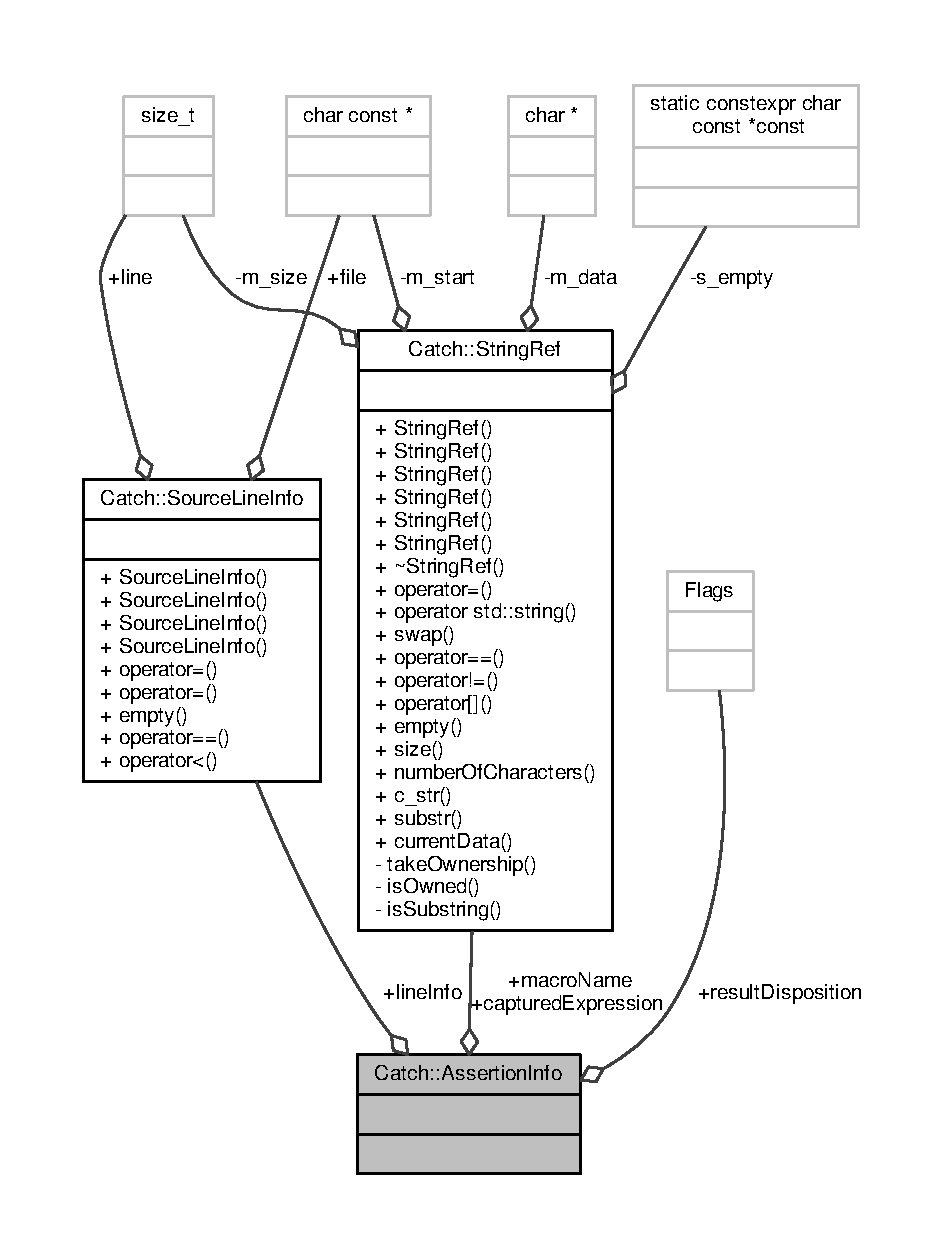
\includegraphics[width=350pt]{struct_catch_1_1_assertion_info__coll__graph}
\end{center}
\end{figure}
\subsection*{Public Attributes}
\begin{DoxyCompactItemize}
\item 
\hyperlink{class_catch_1_1_string_ref}{String\-Ref} \hyperlink{struct_catch_1_1_assertion_info_aaf3fbb9f1fe09c879ba3d877584e3056}{macro\-Name}
\item 
\hyperlink{struct_catch_1_1_source_line_info}{Source\-Line\-Info} \hyperlink{struct_catch_1_1_assertion_info_a17bdbb404ba12658034f833be2f4c3e7}{line\-Info}
\item 
\hyperlink{class_catch_1_1_string_ref}{String\-Ref} \hyperlink{struct_catch_1_1_assertion_info_accd36744b4acaa3a691a72df0b42190f}{captured\-Expression}
\item 
\hyperlink{struct_catch_1_1_result_disposition_a3396cad6e2259af326b3aae93e23e9d8}{Result\-Disposition\-::\-Flags} \hyperlink{struct_catch_1_1_assertion_info_a60353b3632ab2f827162f2b2d6911073}{result\-Disposition}
\end{DoxyCompactItemize}


\subsection{Member Data Documentation}
\hypertarget{struct_catch_1_1_assertion_info_accd36744b4acaa3a691a72df0b42190f}{\index{Catch\-::\-Assertion\-Info@{Catch\-::\-Assertion\-Info}!captured\-Expression@{captured\-Expression}}
\index{captured\-Expression@{captured\-Expression}!Catch::AssertionInfo@{Catch\-::\-Assertion\-Info}}
\subsubsection[{captured\-Expression}]{\setlength{\rightskip}{0pt plus 5cm}{\bf String\-Ref} Catch\-::\-Assertion\-Info\-::captured\-Expression}}\label{struct_catch_1_1_assertion_info_accd36744b4acaa3a691a72df0b42190f}
\hypertarget{struct_catch_1_1_assertion_info_a17bdbb404ba12658034f833be2f4c3e7}{\index{Catch\-::\-Assertion\-Info@{Catch\-::\-Assertion\-Info}!line\-Info@{line\-Info}}
\index{line\-Info@{line\-Info}!Catch::AssertionInfo@{Catch\-::\-Assertion\-Info}}
\subsubsection[{line\-Info}]{\setlength{\rightskip}{0pt plus 5cm}{\bf Source\-Line\-Info} Catch\-::\-Assertion\-Info\-::line\-Info}}\label{struct_catch_1_1_assertion_info_a17bdbb404ba12658034f833be2f4c3e7}
\hypertarget{struct_catch_1_1_assertion_info_aaf3fbb9f1fe09c879ba3d877584e3056}{\index{Catch\-::\-Assertion\-Info@{Catch\-::\-Assertion\-Info}!macro\-Name@{macro\-Name}}
\index{macro\-Name@{macro\-Name}!Catch::AssertionInfo@{Catch\-::\-Assertion\-Info}}
\subsubsection[{macro\-Name}]{\setlength{\rightskip}{0pt plus 5cm}{\bf String\-Ref} Catch\-::\-Assertion\-Info\-::macro\-Name}}\label{struct_catch_1_1_assertion_info_aaf3fbb9f1fe09c879ba3d877584e3056}
\hypertarget{struct_catch_1_1_assertion_info_a60353b3632ab2f827162f2b2d6911073}{\index{Catch\-::\-Assertion\-Info@{Catch\-::\-Assertion\-Info}!result\-Disposition@{result\-Disposition}}
\index{result\-Disposition@{result\-Disposition}!Catch::AssertionInfo@{Catch\-::\-Assertion\-Info}}
\subsubsection[{result\-Disposition}]{\setlength{\rightskip}{0pt plus 5cm}{\bf Result\-Disposition\-::\-Flags} Catch\-::\-Assertion\-Info\-::result\-Disposition}}\label{struct_catch_1_1_assertion_info_a60353b3632ab2f827162f2b2d6911073}


The documentation for this struct was generated from the following file\-:\begin{DoxyCompactItemize}
\item 
\hyperlink{catch_8hpp}{catch.\-hpp}\end{DoxyCompactItemize}

\hypertarget{struct_catch_1_1_assertion_reaction}{\section{Catch\-:\-:Assertion\-Reaction Struct Reference}
\label{struct_catch_1_1_assertion_reaction}\index{Catch\-::\-Assertion\-Reaction@{Catch\-::\-Assertion\-Reaction}}
}


{\ttfamily \#include $<$catch.\-hpp$>$}



Collaboration diagram for Catch\-:\-:Assertion\-Reaction\-:
\nopagebreak
\begin{figure}[H]
\begin{center}
\leavevmode
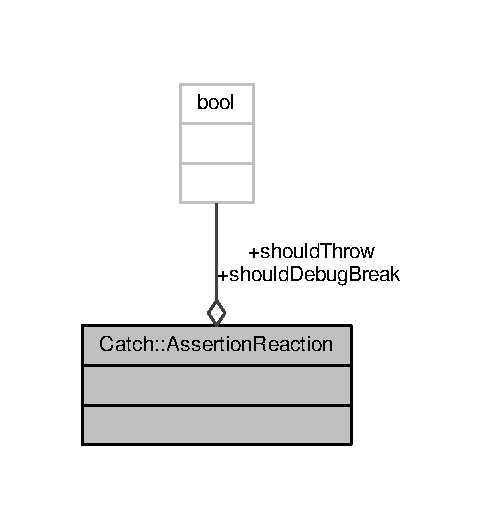
\includegraphics[width=233pt]{struct_catch_1_1_assertion_reaction__coll__graph}
\end{center}
\end{figure}
\subsection*{Public Attributes}
\begin{DoxyCompactItemize}
\item 
bool \hyperlink{struct_catch_1_1_assertion_reaction_adcf30fb90ff20d9789df78d424652497}{should\-Debug\-Break} = false
\item 
bool \hyperlink{struct_catch_1_1_assertion_reaction_a82c8d95a2c1b6a331bde66982a8e090f}{should\-Throw} = false
\end{DoxyCompactItemize}


\subsection{Member Data Documentation}
\hypertarget{struct_catch_1_1_assertion_reaction_adcf30fb90ff20d9789df78d424652497}{\index{Catch\-::\-Assertion\-Reaction@{Catch\-::\-Assertion\-Reaction}!should\-Debug\-Break@{should\-Debug\-Break}}
\index{should\-Debug\-Break@{should\-Debug\-Break}!Catch::AssertionReaction@{Catch\-::\-Assertion\-Reaction}}
\subsubsection[{should\-Debug\-Break}]{\setlength{\rightskip}{0pt plus 5cm}bool Catch\-::\-Assertion\-Reaction\-::should\-Debug\-Break = false}}\label{struct_catch_1_1_assertion_reaction_adcf30fb90ff20d9789df78d424652497}
\hypertarget{struct_catch_1_1_assertion_reaction_a82c8d95a2c1b6a331bde66982a8e090f}{\index{Catch\-::\-Assertion\-Reaction@{Catch\-::\-Assertion\-Reaction}!should\-Throw@{should\-Throw}}
\index{should\-Throw@{should\-Throw}!Catch::AssertionReaction@{Catch\-::\-Assertion\-Reaction}}
\subsubsection[{should\-Throw}]{\setlength{\rightskip}{0pt plus 5cm}bool Catch\-::\-Assertion\-Reaction\-::should\-Throw = false}}\label{struct_catch_1_1_assertion_reaction_a82c8d95a2c1b6a331bde66982a8e090f}


The documentation for this struct was generated from the following file\-:\begin{DoxyCompactItemize}
\item 
\hyperlink{catch_8hpp}{catch.\-hpp}\end{DoxyCompactItemize}

\hypertarget{struct_catch_1_1_auto_reg}{\section{Catch\-:\-:Auto\-Reg Struct Reference}
\label{struct_catch_1_1_auto_reg}\index{Catch\-::\-Auto\-Reg@{Catch\-::\-Auto\-Reg}}
}


{\ttfamily \#include $<$catch.\-hpp$>$}



Inheritance diagram for Catch\-:\-:Auto\-Reg\-:
\nopagebreak
\begin{figure}[H]
\begin{center}
\leavevmode
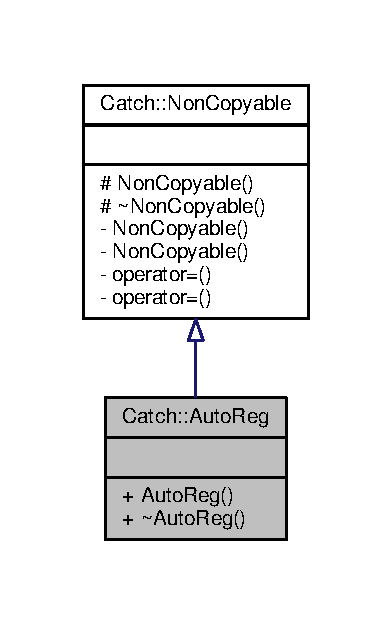
\includegraphics[width=188pt]{struct_catch_1_1_auto_reg__inherit__graph}
\end{center}
\end{figure}


Collaboration diagram for Catch\-:\-:Auto\-Reg\-:
\nopagebreak
\begin{figure}[H]
\begin{center}
\leavevmode
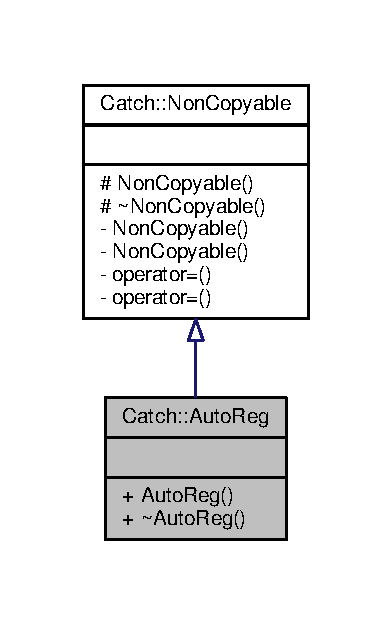
\includegraphics[width=188pt]{struct_catch_1_1_auto_reg__coll__graph}
\end{center}
\end{figure}
\subsection*{Public Member Functions}
\begin{DoxyCompactItemize}
\item 
\hyperlink{struct_catch_1_1_auto_reg_a7eba02fb9d80b9896bf5a6517369af28}{Auto\-Reg} (\hyperlink{struct_catch_1_1_i_test_invoker}{I\-Test\-Invoker} $\ast$invoker, \hyperlink{struct_catch_1_1_source_line_info}{Source\-Line\-Info} const \&line\-Info, \hyperlink{class_catch_1_1_string_ref}{String\-Ref} const \&class\-Or\-Method, \hyperlink{struct_catch_1_1_name_and_tags}{Name\-And\-Tags} const \&name\-And\-Tags) noexcept
\item 
\hyperlink{struct_catch_1_1_auto_reg_a3cdb53f1e5ff115310f3372bebe198f1}{$\sim$\-Auto\-Reg} ()
\end{DoxyCompactItemize}
\subsection*{Additional Inherited Members}


\subsection{Constructor \& Destructor Documentation}
\hypertarget{struct_catch_1_1_auto_reg_a7eba02fb9d80b9896bf5a6517369af28}{\index{Catch\-::\-Auto\-Reg@{Catch\-::\-Auto\-Reg}!Auto\-Reg@{Auto\-Reg}}
\index{Auto\-Reg@{Auto\-Reg}!Catch::AutoReg@{Catch\-::\-Auto\-Reg}}
\subsubsection[{Auto\-Reg}]{\setlength{\rightskip}{0pt plus 5cm}Catch\-::\-Auto\-Reg\-::\-Auto\-Reg (
\begin{DoxyParamCaption}
\item[{{\bf I\-Test\-Invoker} $\ast$}]{invoker, }
\item[{{\bf Source\-Line\-Info} const \&}]{line\-Info, }
\item[{{\bf String\-Ref} const \&}]{class\-Or\-Method, }
\item[{{\bf Name\-And\-Tags} const \&}]{name\-And\-Tags}
\end{DoxyParamCaption}
)\hspace{0.3cm}{\ttfamily [noexcept]}}}\label{struct_catch_1_1_auto_reg_a7eba02fb9d80b9896bf5a6517369af28}
\hypertarget{struct_catch_1_1_auto_reg_a3cdb53f1e5ff115310f3372bebe198f1}{\index{Catch\-::\-Auto\-Reg@{Catch\-::\-Auto\-Reg}!$\sim$\-Auto\-Reg@{$\sim$\-Auto\-Reg}}
\index{$\sim$\-Auto\-Reg@{$\sim$\-Auto\-Reg}!Catch::AutoReg@{Catch\-::\-Auto\-Reg}}
\subsubsection[{$\sim$\-Auto\-Reg}]{\setlength{\rightskip}{0pt plus 5cm}Catch\-::\-Auto\-Reg\-::$\sim$\-Auto\-Reg (
\begin{DoxyParamCaption}
{}
\end{DoxyParamCaption}
)}}\label{struct_catch_1_1_auto_reg_a3cdb53f1e5ff115310f3372bebe198f1}


The documentation for this struct was generated from the following file\-:\begin{DoxyCompactItemize}
\item 
\hyperlink{catch_8hpp}{catch.\-hpp}\end{DoxyCompactItemize}

\hypertarget{class_catch_1_1_benchmark_looper}{\section{Catch\-:\-:Benchmark\-Looper Class Reference}
\label{class_catch_1_1_benchmark_looper}\index{Catch\-::\-Benchmark\-Looper@{Catch\-::\-Benchmark\-Looper}}
}


{\ttfamily \#include $<$catch.\-hpp$>$}



Collaboration diagram for Catch\-:\-:Benchmark\-Looper\-:
\nopagebreak
\begin{figure}[H]
\begin{center}
\leavevmode
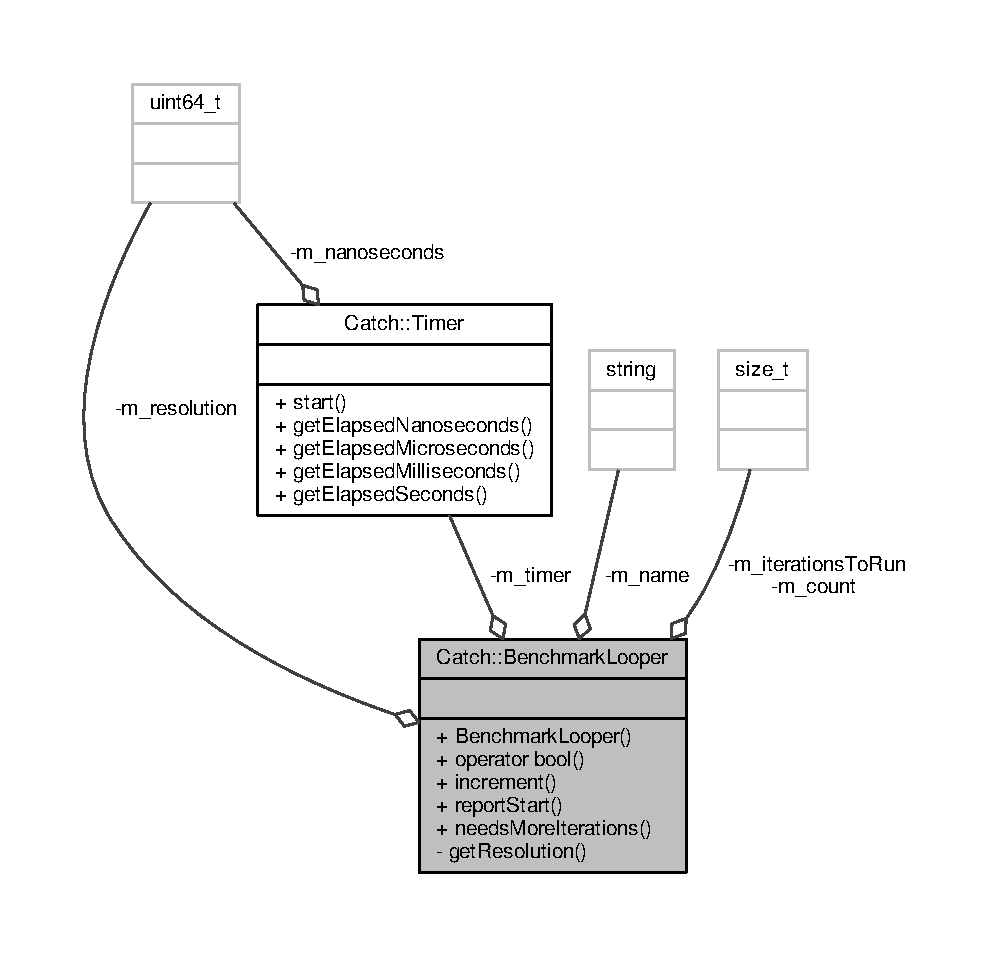
\includegraphics[width=350pt]{class_catch_1_1_benchmark_looper__coll__graph}
\end{center}
\end{figure}
\subsection*{Public Member Functions}
\begin{DoxyCompactItemize}
\item 
\hyperlink{class_catch_1_1_benchmark_looper_ab9ba6397306a70082f39e63a8a71bde6}{Benchmark\-Looper} (\hyperlink{class_catch_1_1_string_ref}{String\-Ref} name)
\item 
\hyperlink{class_catch_1_1_benchmark_looper_a54da41bada9da038dc05faf41d746765}{operator bool} ()
\item 
void \hyperlink{class_catch_1_1_benchmark_looper_a210552aff5b19408637444d4bb35d59c}{increment} ()
\item 
void \hyperlink{class_catch_1_1_benchmark_looper_a0697d1b266112b110edf2025b82c4e77}{report\-Start} ()
\item 
auto \hyperlink{class_catch_1_1_benchmark_looper_a97bd944521f519b1593a5d1d2f9998fa}{needs\-More\-Iterations} () -\/$>$ bool
\end{DoxyCompactItemize}
\subsection*{Static Private Member Functions}
\begin{DoxyCompactItemize}
\item 
static auto \hyperlink{class_catch_1_1_benchmark_looper_a45fd79f05ac1fb21dcfb3a81cf052705}{get\-Resolution} () -\/$>$ uint64\-\_\-t
\end{DoxyCompactItemize}
\subsection*{Private Attributes}
\begin{DoxyCompactItemize}
\item 
std\-::string \hyperlink{class_catch_1_1_benchmark_looper_afa2005187a2abbcae69a5b16c89e68c3}{m\-\_\-name}
\item 
std\-::size\-\_\-t \hyperlink{class_catch_1_1_benchmark_looper_aae36ced9e5b1c884e2b3ac9d04c1c373}{m\-\_\-count} = 0
\item 
std\-::size\-\_\-t \hyperlink{class_catch_1_1_benchmark_looper_af28bef6706fe983afca85d2ccd2b6ca8}{m\-\_\-iterations\-To\-Run} = 1
\item 
uint64\-\_\-t \hyperlink{class_catch_1_1_benchmark_looper_a7e7168e3d346e78d6e85c810aec6a55d}{m\-\_\-resolution}
\item 
\hyperlink{class_catch_1_1_timer}{Timer} \hyperlink{class_catch_1_1_benchmark_looper_af86aacecba12576f96a1d3f321a0c959}{m\-\_\-timer}
\end{DoxyCompactItemize}


\subsection{Constructor \& Destructor Documentation}
\hypertarget{class_catch_1_1_benchmark_looper_ab9ba6397306a70082f39e63a8a71bde6}{\index{Catch\-::\-Benchmark\-Looper@{Catch\-::\-Benchmark\-Looper}!Benchmark\-Looper@{Benchmark\-Looper}}
\index{Benchmark\-Looper@{Benchmark\-Looper}!Catch::BenchmarkLooper@{Catch\-::\-Benchmark\-Looper}}
\subsubsection[{Benchmark\-Looper}]{\setlength{\rightskip}{0pt plus 5cm}Catch\-::\-Benchmark\-Looper\-::\-Benchmark\-Looper (
\begin{DoxyParamCaption}
\item[{{\bf String\-Ref}}]{name}
\end{DoxyParamCaption}
)\hspace{0.3cm}{\ttfamily [inline]}}}\label{class_catch_1_1_benchmark_looper_ab9ba6397306a70082f39e63a8a71bde6}

\begin{DoxyCode}
1915             : \hyperlink{class_catch_1_1_benchmark_looper_afa2005187a2abbcae69a5b16c89e68c3}{m\_name}(name),
1916             \hyperlink{class_catch_1_1_benchmark_looper_a7e7168e3d346e78d6e85c810aec6a55d}{m\_resolution}(\hyperlink{class_catch_1_1_benchmark_looper_a45fd79f05ac1fb21dcfb3a81cf052705}{getResolution}())
1917         \{
1918             \hyperlink{class_catch_1_1_benchmark_looper_a0697d1b266112b110edf2025b82c4e77}{reportStart}();
1919             \hyperlink{class_catch_1_1_benchmark_looper_af86aacecba12576f96a1d3f321a0c959}{m\_timer}.\hyperlink{class_catch_1_1_timer_a0a56e879e43f36c102bf9ea8b5fc8b72}{start}();
1920         \}
\end{DoxyCode}


\subsection{Member Function Documentation}
\hypertarget{class_catch_1_1_benchmark_looper_a45fd79f05ac1fb21dcfb3a81cf052705}{\index{Catch\-::\-Benchmark\-Looper@{Catch\-::\-Benchmark\-Looper}!get\-Resolution@{get\-Resolution}}
\index{get\-Resolution@{get\-Resolution}!Catch::BenchmarkLooper@{Catch\-::\-Benchmark\-Looper}}
\subsubsection[{get\-Resolution}]{\setlength{\rightskip}{0pt plus 5cm}static auto Catch\-::\-Benchmark\-Looper\-::get\-Resolution (
\begin{DoxyParamCaption}
{}
\end{DoxyParamCaption}
) -\/$>$  uint64\-\_\-t\hspace{0.3cm}{\ttfamily [static]}, {\ttfamily [private]}}}\label{class_catch_1_1_benchmark_looper_a45fd79f05ac1fb21dcfb3a81cf052705}
\hypertarget{class_catch_1_1_benchmark_looper_a210552aff5b19408637444d4bb35d59c}{\index{Catch\-::\-Benchmark\-Looper@{Catch\-::\-Benchmark\-Looper}!increment@{increment}}
\index{increment@{increment}!Catch::BenchmarkLooper@{Catch\-::\-Benchmark\-Looper}}
\subsubsection[{increment}]{\setlength{\rightskip}{0pt plus 5cm}void Catch\-::\-Benchmark\-Looper\-::increment (
\begin{DoxyParamCaption}
{}
\end{DoxyParamCaption}
)\hspace{0.3cm}{\ttfamily [inline]}}}\label{class_catch_1_1_benchmark_looper_a210552aff5b19408637444d4bb35d59c}

\begin{DoxyCode}
1928                          \{
1929             ++\hyperlink{class_catch_1_1_benchmark_looper_aae36ced9e5b1c884e2b3ac9d04c1c373}{m\_count};
1930         \}
\end{DoxyCode}
\hypertarget{class_catch_1_1_benchmark_looper_a97bd944521f519b1593a5d1d2f9998fa}{\index{Catch\-::\-Benchmark\-Looper@{Catch\-::\-Benchmark\-Looper}!needs\-More\-Iterations@{needs\-More\-Iterations}}
\index{needs\-More\-Iterations@{needs\-More\-Iterations}!Catch::BenchmarkLooper@{Catch\-::\-Benchmark\-Looper}}
\subsubsection[{needs\-More\-Iterations}]{\setlength{\rightskip}{0pt plus 5cm}auto Catch\-::\-Benchmark\-Looper\-::needs\-More\-Iterations (
\begin{DoxyParamCaption}
{}
\end{DoxyParamCaption}
) -\/$>$  bool}}\label{class_catch_1_1_benchmark_looper_a97bd944521f519b1593a5d1d2f9998fa}
\hypertarget{class_catch_1_1_benchmark_looper_a54da41bada9da038dc05faf41d746765}{\index{Catch\-::\-Benchmark\-Looper@{Catch\-::\-Benchmark\-Looper}!operator bool@{operator bool}}
\index{operator bool@{operator bool}!Catch::BenchmarkLooper@{Catch\-::\-Benchmark\-Looper}}
\subsubsection[{operator bool}]{\setlength{\rightskip}{0pt plus 5cm}Catch\-::\-Benchmark\-Looper\-::operator bool (
\begin{DoxyParamCaption}
{}
\end{DoxyParamCaption}
)\hspace{0.3cm}{\ttfamily [inline]}, {\ttfamily [explicit]}}}\label{class_catch_1_1_benchmark_looper_a54da41bada9da038dc05faf41d746765}

\begin{DoxyCode}
1922                                  \{
1923             \textcolor{keywordflow}{if} (\hyperlink{class_catch_1_1_benchmark_looper_aae36ced9e5b1c884e2b3ac9d04c1c373}{m\_count} < \hyperlink{class_catch_1_1_benchmark_looper_af28bef6706fe983afca85d2ccd2b6ca8}{m\_iterationsToRun})
1924                 \textcolor{keywordflow}{return} \textcolor{keyword}{true};
1925             \textcolor{keywordflow}{return} \hyperlink{class_catch_1_1_benchmark_looper_a97bd944521f519b1593a5d1d2f9998fa}{needsMoreIterations}();
1926         \}
\end{DoxyCode}
\hypertarget{class_catch_1_1_benchmark_looper_a0697d1b266112b110edf2025b82c4e77}{\index{Catch\-::\-Benchmark\-Looper@{Catch\-::\-Benchmark\-Looper}!report\-Start@{report\-Start}}
\index{report\-Start@{report\-Start}!Catch::BenchmarkLooper@{Catch\-::\-Benchmark\-Looper}}
\subsubsection[{report\-Start}]{\setlength{\rightskip}{0pt plus 5cm}void Catch\-::\-Benchmark\-Looper\-::report\-Start (
\begin{DoxyParamCaption}
{}
\end{DoxyParamCaption}
)}}\label{class_catch_1_1_benchmark_looper_a0697d1b266112b110edf2025b82c4e77}


\subsection{Member Data Documentation}
\hypertarget{class_catch_1_1_benchmark_looper_aae36ced9e5b1c884e2b3ac9d04c1c373}{\index{Catch\-::\-Benchmark\-Looper@{Catch\-::\-Benchmark\-Looper}!m\-\_\-count@{m\-\_\-count}}
\index{m\-\_\-count@{m\-\_\-count}!Catch::BenchmarkLooper@{Catch\-::\-Benchmark\-Looper}}
\subsubsection[{m\-\_\-count}]{\setlength{\rightskip}{0pt plus 5cm}std\-::size\-\_\-t Catch\-::\-Benchmark\-Looper\-::m\-\_\-count = 0\hspace{0.3cm}{\ttfamily [private]}}}\label{class_catch_1_1_benchmark_looper_aae36ced9e5b1c884e2b3ac9d04c1c373}
\hypertarget{class_catch_1_1_benchmark_looper_af28bef6706fe983afca85d2ccd2b6ca8}{\index{Catch\-::\-Benchmark\-Looper@{Catch\-::\-Benchmark\-Looper}!m\-\_\-iterations\-To\-Run@{m\-\_\-iterations\-To\-Run}}
\index{m\-\_\-iterations\-To\-Run@{m\-\_\-iterations\-To\-Run}!Catch::BenchmarkLooper@{Catch\-::\-Benchmark\-Looper}}
\subsubsection[{m\-\_\-iterations\-To\-Run}]{\setlength{\rightskip}{0pt plus 5cm}std\-::size\-\_\-t Catch\-::\-Benchmark\-Looper\-::m\-\_\-iterations\-To\-Run = 1\hspace{0.3cm}{\ttfamily [private]}}}\label{class_catch_1_1_benchmark_looper_af28bef6706fe983afca85d2ccd2b6ca8}
\hypertarget{class_catch_1_1_benchmark_looper_afa2005187a2abbcae69a5b16c89e68c3}{\index{Catch\-::\-Benchmark\-Looper@{Catch\-::\-Benchmark\-Looper}!m\-\_\-name@{m\-\_\-name}}
\index{m\-\_\-name@{m\-\_\-name}!Catch::BenchmarkLooper@{Catch\-::\-Benchmark\-Looper}}
\subsubsection[{m\-\_\-name}]{\setlength{\rightskip}{0pt plus 5cm}std\-::string Catch\-::\-Benchmark\-Looper\-::m\-\_\-name\hspace{0.3cm}{\ttfamily [private]}}}\label{class_catch_1_1_benchmark_looper_afa2005187a2abbcae69a5b16c89e68c3}
\hypertarget{class_catch_1_1_benchmark_looper_a7e7168e3d346e78d6e85c810aec6a55d}{\index{Catch\-::\-Benchmark\-Looper@{Catch\-::\-Benchmark\-Looper}!m\-\_\-resolution@{m\-\_\-resolution}}
\index{m\-\_\-resolution@{m\-\_\-resolution}!Catch::BenchmarkLooper@{Catch\-::\-Benchmark\-Looper}}
\subsubsection[{m\-\_\-resolution}]{\setlength{\rightskip}{0pt plus 5cm}uint64\-\_\-t Catch\-::\-Benchmark\-Looper\-::m\-\_\-resolution\hspace{0.3cm}{\ttfamily [private]}}}\label{class_catch_1_1_benchmark_looper_a7e7168e3d346e78d6e85c810aec6a55d}
\hypertarget{class_catch_1_1_benchmark_looper_af86aacecba12576f96a1d3f321a0c959}{\index{Catch\-::\-Benchmark\-Looper@{Catch\-::\-Benchmark\-Looper}!m\-\_\-timer@{m\-\_\-timer}}
\index{m\-\_\-timer@{m\-\_\-timer}!Catch::BenchmarkLooper@{Catch\-::\-Benchmark\-Looper}}
\subsubsection[{m\-\_\-timer}]{\setlength{\rightskip}{0pt plus 5cm}{\bf Timer} Catch\-::\-Benchmark\-Looper\-::m\-\_\-timer\hspace{0.3cm}{\ttfamily [private]}}}\label{class_catch_1_1_benchmark_looper_af86aacecba12576f96a1d3f321a0c959}


The documentation for this class was generated from the following file\-:\begin{DoxyCompactItemize}
\item 
\hyperlink{catch_8hpp}{catch.\-hpp}\end{DoxyCompactItemize}

\hypertarget{class_catch_1_1_binary_expr}{\section{Catch\-:\-:Binary\-Expr$<$ Lhs\-T, Rhs\-T $>$ Class Template Reference}
\label{class_catch_1_1_binary_expr}\index{Catch\-::\-Binary\-Expr$<$ Lhs\-T, Rhs\-T $>$@{Catch\-::\-Binary\-Expr$<$ Lhs\-T, Rhs\-T $>$}}
}


{\ttfamily \#include $<$catch.\-hpp$>$}



Inheritance diagram for Catch\-:\-:Binary\-Expr$<$ Lhs\-T, Rhs\-T $>$\-:
\nopagebreak
\begin{figure}[H]
\begin{center}
\leavevmode
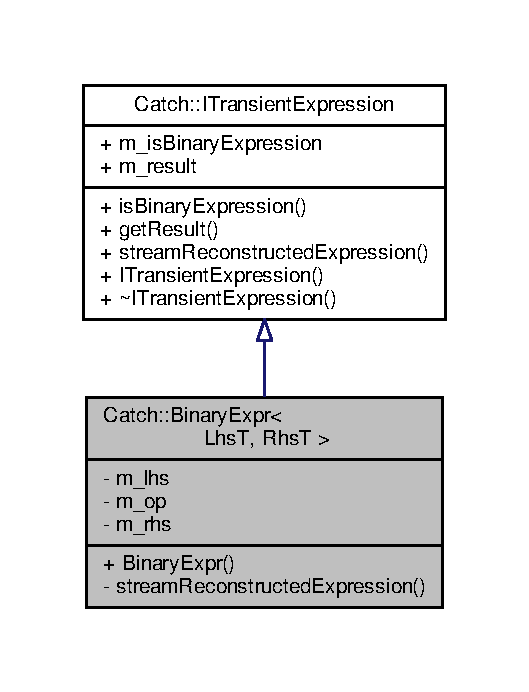
\includegraphics[width=254pt]{class_catch_1_1_binary_expr__inherit__graph}
\end{center}
\end{figure}


Collaboration diagram for Catch\-:\-:Binary\-Expr$<$ Lhs\-T, Rhs\-T $>$\-:
\nopagebreak
\begin{figure}[H]
\begin{center}
\leavevmode
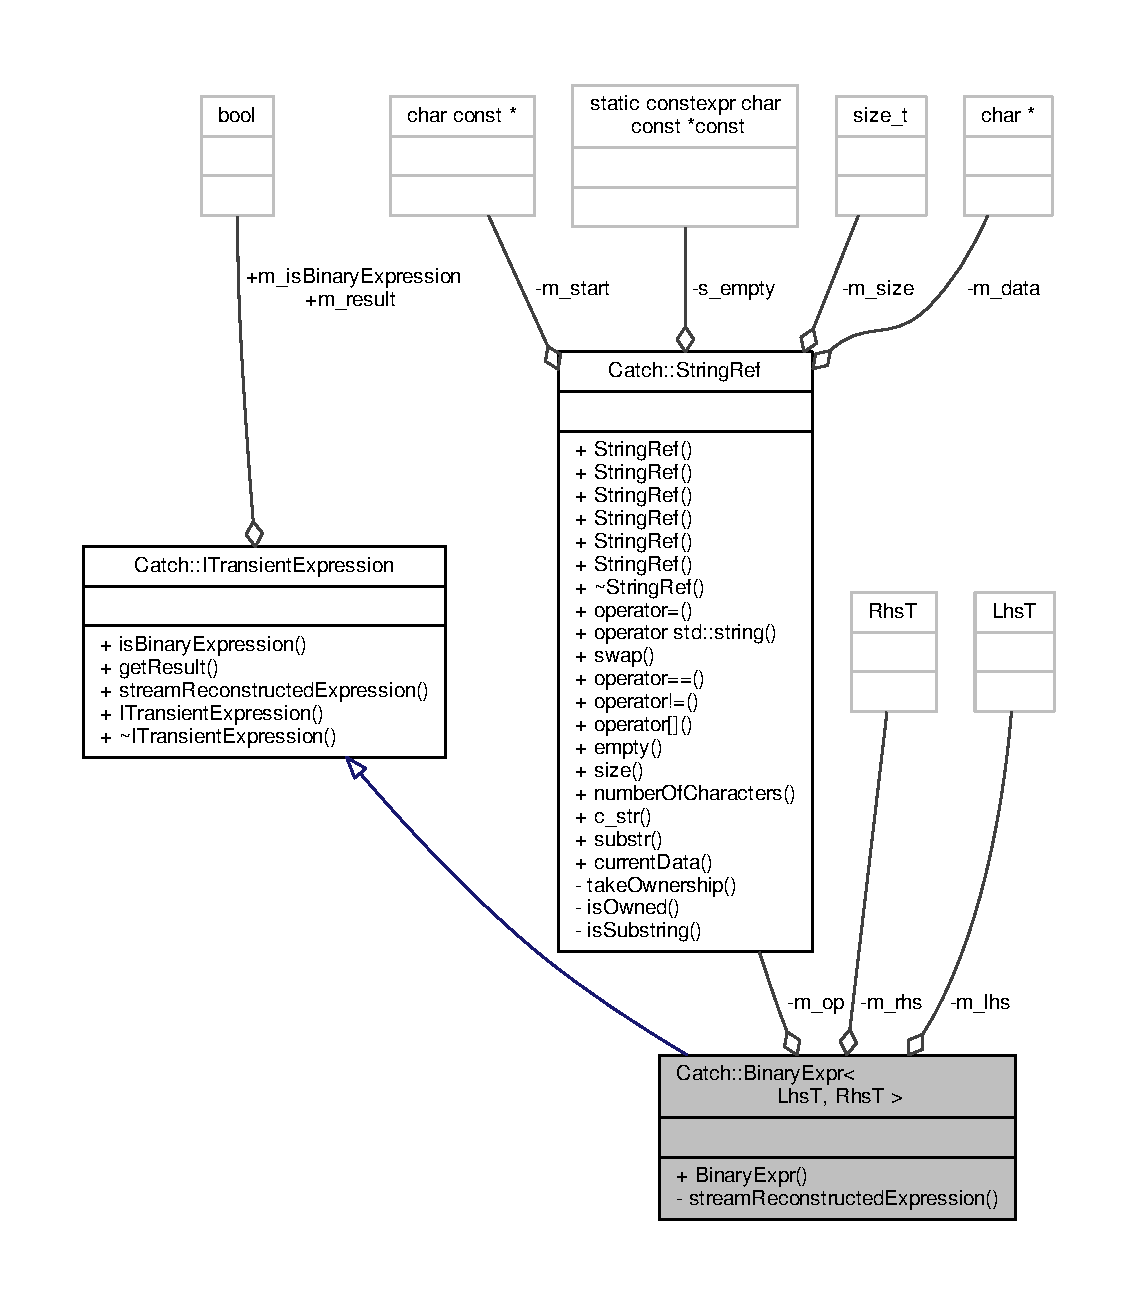
\includegraphics[width=350pt]{class_catch_1_1_binary_expr__coll__graph}
\end{center}
\end{figure}
\subsection*{Public Member Functions}
\begin{DoxyCompactItemize}
\item 
\hyperlink{class_catch_1_1_binary_expr_a657d66346aef97a760c22776fe6008b6}{Binary\-Expr} (bool comparison\-Result, Lhs\-T lhs, \hyperlink{class_catch_1_1_string_ref}{String\-Ref} op, Rhs\-T rhs)
\end{DoxyCompactItemize}
\subsection*{Private Member Functions}
\begin{DoxyCompactItemize}
\item 
void \hyperlink{class_catch_1_1_binary_expr_af998022712d4bd3e4fc7ab9b8a38b445}{stream\-Reconstructed\-Expression} (std\-::ostream \&os) const override
\end{DoxyCompactItemize}
\subsection*{Private Attributes}
\begin{DoxyCompactItemize}
\item 
Lhs\-T \hyperlink{class_catch_1_1_binary_expr_a306b29e77b48f9c538c5031a59adc4ce}{m\-\_\-lhs}
\item 
\hyperlink{class_catch_1_1_string_ref}{String\-Ref} \hyperlink{class_catch_1_1_binary_expr_ab21dea40c53fd64d4f7a073dbe93ec95}{m\-\_\-op}
\item 
Rhs\-T \hyperlink{class_catch_1_1_binary_expr_a54cb1629bf304ebe0c1560f4cc2bc186}{m\-\_\-rhs}
\end{DoxyCompactItemize}
\subsection*{Additional Inherited Members}


\subsection{Constructor \& Destructor Documentation}
\hypertarget{class_catch_1_1_binary_expr_a657d66346aef97a760c22776fe6008b6}{\index{Catch\-::\-Binary\-Expr@{Catch\-::\-Binary\-Expr}!Binary\-Expr@{Binary\-Expr}}
\index{Binary\-Expr@{Binary\-Expr}!Catch::BinaryExpr@{Catch\-::\-Binary\-Expr}}
\subsubsection[{Binary\-Expr}]{\setlength{\rightskip}{0pt plus 5cm}template$<$typename Lhs\-T , typename Rhs\-T $>$ {\bf Catch\-::\-Binary\-Expr}$<$ Lhs\-T, Rhs\-T $>$\-::{\bf Binary\-Expr} (
\begin{DoxyParamCaption}
\item[{bool}]{comparison\-Result, }
\item[{Lhs\-T}]{lhs, }
\item[{{\bf String\-Ref}}]{op, }
\item[{Rhs\-T}]{rhs}
\end{DoxyParamCaption}
)\hspace{0.3cm}{\ttfamily [inline]}}}\label{class_catch_1_1_binary_expr_a657d66346aef97a760c22776fe6008b6}

\begin{DoxyCode}
1335             : \hyperlink{struct_catch_1_1_i_transient_expression_aafe69572b7ed884e63ec81f58d4afd8c}{ITransientExpression}\{ \textcolor{keyword}{true}, comparisonResult \},
1336             \hyperlink{class_catch_1_1_binary_expr_a306b29e77b48f9c538c5031a59adc4ce}{m\_lhs}(lhs),
1337             \hyperlink{class_catch_1_1_binary_expr_ab21dea40c53fd64d4f7a073dbe93ec95}{m\_op}(op),
1338             \hyperlink{class_catch_1_1_binary_expr_a54cb1629bf304ebe0c1560f4cc2bc186}{m\_rhs}(rhs)
1339         \{\}
\end{DoxyCode}


\subsection{Member Function Documentation}
\hypertarget{class_catch_1_1_binary_expr_af998022712d4bd3e4fc7ab9b8a38b445}{\index{Catch\-::\-Binary\-Expr@{Catch\-::\-Binary\-Expr}!stream\-Reconstructed\-Expression@{stream\-Reconstructed\-Expression}}
\index{stream\-Reconstructed\-Expression@{stream\-Reconstructed\-Expression}!Catch::BinaryExpr@{Catch\-::\-Binary\-Expr}}
\subsubsection[{stream\-Reconstructed\-Expression}]{\setlength{\rightskip}{0pt plus 5cm}template$<$typename Lhs\-T , typename Rhs\-T $>$ void {\bf Catch\-::\-Binary\-Expr}$<$ Lhs\-T, Rhs\-T $>$\-::stream\-Reconstructed\-Expression (
\begin{DoxyParamCaption}
\item[{std\-::ostream \&}]{os}
\end{DoxyParamCaption}
) const\hspace{0.3cm}{\ttfamily [inline]}, {\ttfamily [override]}, {\ttfamily [private]}, {\ttfamily [virtual]}}}\label{class_catch_1_1_binary_expr_af998022712d4bd3e4fc7ab9b8a38b445}


Implements \hyperlink{struct_catch_1_1_i_transient_expression_aabe1889df9c6e639a24afb08d8a0fe9e}{Catch\-::\-I\-Transient\-Expression}.



References Catch\-::format\-Reconstructed\-Expression(), and Catch\-::\-Detail\-::stringify().


\begin{DoxyCode}
1328                                                                           \{
1329             \hyperlink{namespace_catch_a520110c31f26cf9892595772ab814fc0}{formatReconstructedExpression}
1330             (os, \hyperlink{namespace_catch_1_1_detail_af0ad48344ffd3f92f3568465248a9880}{Catch::Detail::stringify}(\hyperlink{class_catch_1_1_binary_expr_a306b29e77b48f9c538c5031a59adc4ce}{m\_lhs}), 
      \hyperlink{class_catch_1_1_binary_expr_ab21dea40c53fd64d4f7a073dbe93ec95}{m\_op}, \hyperlink{namespace_catch_1_1_detail_af0ad48344ffd3f92f3568465248a9880}{Catch::Detail::stringify}(\hyperlink{class_catch_1_1_binary_expr_a54cb1629bf304ebe0c1560f4cc2bc186}{m\_rhs}));
1331         \}
\end{DoxyCode}


\subsection{Member Data Documentation}
\hypertarget{class_catch_1_1_binary_expr_a306b29e77b48f9c538c5031a59adc4ce}{\index{Catch\-::\-Binary\-Expr@{Catch\-::\-Binary\-Expr}!m\-\_\-lhs@{m\-\_\-lhs}}
\index{m\-\_\-lhs@{m\-\_\-lhs}!Catch::BinaryExpr@{Catch\-::\-Binary\-Expr}}
\subsubsection[{m\-\_\-lhs}]{\setlength{\rightskip}{0pt plus 5cm}template$<$typename Lhs\-T , typename Rhs\-T $>$ Lhs\-T {\bf Catch\-::\-Binary\-Expr}$<$ Lhs\-T, Rhs\-T $>$\-::m\-\_\-lhs\hspace{0.3cm}{\ttfamily [private]}}}\label{class_catch_1_1_binary_expr_a306b29e77b48f9c538c5031a59adc4ce}
\hypertarget{class_catch_1_1_binary_expr_ab21dea40c53fd64d4f7a073dbe93ec95}{\index{Catch\-::\-Binary\-Expr@{Catch\-::\-Binary\-Expr}!m\-\_\-op@{m\-\_\-op}}
\index{m\-\_\-op@{m\-\_\-op}!Catch::BinaryExpr@{Catch\-::\-Binary\-Expr}}
\subsubsection[{m\-\_\-op}]{\setlength{\rightskip}{0pt plus 5cm}template$<$typename Lhs\-T , typename Rhs\-T $>$ {\bf String\-Ref} {\bf Catch\-::\-Binary\-Expr}$<$ Lhs\-T, Rhs\-T $>$\-::m\-\_\-op\hspace{0.3cm}{\ttfamily [private]}}}\label{class_catch_1_1_binary_expr_ab21dea40c53fd64d4f7a073dbe93ec95}
\hypertarget{class_catch_1_1_binary_expr_a54cb1629bf304ebe0c1560f4cc2bc186}{\index{Catch\-::\-Binary\-Expr@{Catch\-::\-Binary\-Expr}!m\-\_\-rhs@{m\-\_\-rhs}}
\index{m\-\_\-rhs@{m\-\_\-rhs}!Catch::BinaryExpr@{Catch\-::\-Binary\-Expr}}
\subsubsection[{m\-\_\-rhs}]{\setlength{\rightskip}{0pt plus 5cm}template$<$typename Lhs\-T , typename Rhs\-T $>$ Rhs\-T {\bf Catch\-::\-Binary\-Expr}$<$ Lhs\-T, Rhs\-T $>$\-::m\-\_\-rhs\hspace{0.3cm}{\ttfamily [private]}}}\label{class_catch_1_1_binary_expr_a54cb1629bf304ebe0c1560f4cc2bc186}


The documentation for this class was generated from the following file\-:\begin{DoxyCompactItemize}
\item 
\hyperlink{catch_8hpp}{catch.\-hpp}\end{DoxyCompactItemize}

\hypertarget{class_bullet}{\section{Bullet Class Reference}
\label{class_bullet}\index{Bullet@{Bullet}}
}




  




{\ttfamily \#include $<$Bullet.\-h$>$}



Collaboration diagram for Bullet\-:
\nopagebreak
\begin{figure}[H]
\begin{center}
\leavevmode
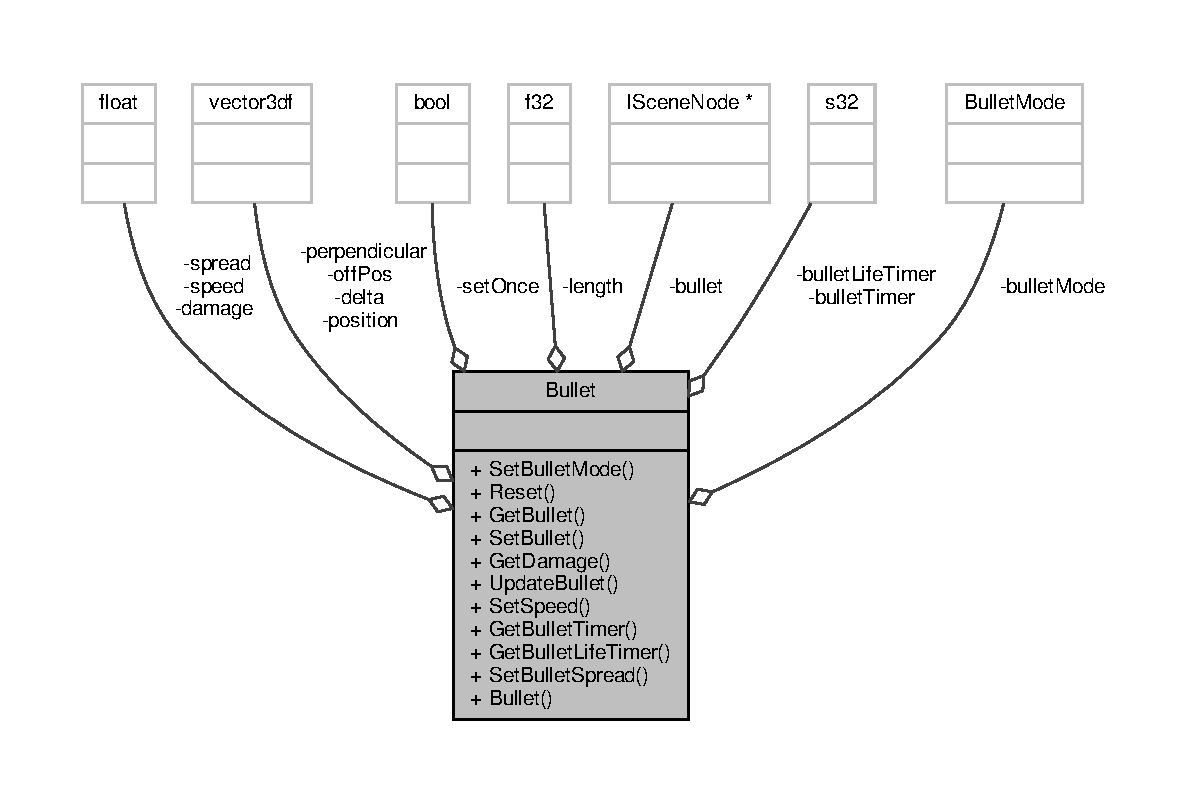
\includegraphics[width=350pt]{class_bullet__coll__graph}
\end{center}
\end{figure}
\subsection*{Public Types}
\begin{DoxyCompactItemize}
\item 
enum \hyperlink{class_bullet_a5d75af562dbb5f6f4f68584ca9193aa5}{Bullet\-Mode} \{ \hyperlink{class_bullet_a5d75af562dbb5f6f4f68584ca9193aa5ab15c8d61fdbcf364ff659250cfff9d3d}{basic}, 
\hyperlink{class_bullet_a5d75af562dbb5f6f4f68584ca9193aa5a6eae620163c016a1c99d33efa49d5b98}{rapid\-Fire}, 
\hyperlink{class_bullet_a5d75af562dbb5f6f4f68584ca9193aa5a70b93c5ed87213fabada7bf06009499a}{split\-Fire}, 
\hyperlink{class_bullet_a5d75af562dbb5f6f4f68584ca9193aa5acbc3fe102aee0027cf26135962ff7fc7}{rapid\-Split\-Fire}
 \}
\begin{DoxyCompactList}\small\item\em \hyperlink{class_bullet}{Bullet} Modes. \end{DoxyCompactList}\end{DoxyCompactItemize}
\subsection*{Public Member Functions}
\begin{DoxyCompactItemize}
\item 
void \hyperlink{class_bullet_a9988e27a0327a7ebca6b407c59661a54}{Set\-Bullet\-Mode} (\hyperlink{class_bullet_a5d75af562dbb5f6f4f68584ca9193aa5}{Bullet\-Mode} mode)
\begin{DoxyCompactList}\small\item\em Set the \hyperlink{class_bullet}{Bullet} Mode. \end{DoxyCompactList}\item 
void \hyperlink{class_bullet_a2de1bc8fb8c70cce09385efd11e9156c}{Reset} ()
\begin{DoxyCompactList}\small\item\em Resets this object. \end{DoxyCompactList}\item 
irr\-::scene\-::\-I\-Scene\-Node $\ast$ \hyperlink{class_bullet_ab9ae469bacf54dfaa69e94b9ead0a908}{Get\-Bullet} ()
\begin{DoxyCompactList}\small\item\em Gets the bullet. \end{DoxyCompactList}\item 
void \hyperlink{class_bullet_a6b68bd110c7a9729c76ae4dc9906e7e7}{Set\-Bullet} (irr\-::scene\-::\-I\-Scene\-Node $\ast$new\-Bullet)
\begin{DoxyCompactList}\small\item\em Sets a bullet. \end{DoxyCompactList}\item 
float \hyperlink{class_bullet_a1fed697f50973eae024e1ce9deeb0442}{Get\-Damage} ()
\begin{DoxyCompactList}\small\item\em Gets the damage. \end{DoxyCompactList}\item 
void \hyperlink{class_bullet_a22c11bea0caf412bcc62ddf13dc541c7}{Update\-Bullet} (irr\-::core\-::vector3df mouse\-Pos, irr\-::core\-::vector3df player\-Pos, float \hyperlink{_player_8cpp_adc988571147642cda93afbf89783f9c9}{frame\-Delta\-Time})
\begin{DoxyCompactList}\small\item\em Updates the bullet. \end{DoxyCompactList}\item 
void \hyperlink{class_bullet_a7a2e293d6bc42d3b018815a0302a0074}{Set\-Speed} (float s)
\begin{DoxyCompactList}\small\item\em Sets the bullet speed. \end{DoxyCompactList}\item 
irr\-::s32 \hyperlink{class_bullet_a5cc762f8b276d0ad812ed3b1fc411626}{Get\-Bullet\-Timer} ()
\begin{DoxyCompactList}\small\item\em Default constructor. \end{DoxyCompactList}\item 
irr\-::s32 \hyperlink{class_bullet_a62aadef0cc64e5ae9085cc4e0267e920}{Get\-Bullet\-Life\-Timer} ()
\item 
void \hyperlink{class_bullet_a1fd596da19949b3dfdba7febd1b162f1}{Set\-Bullet\-Spread} (float s)
\item 
\hyperlink{class_bullet_acd7befc0bc18907cc1d871d37bbdddeb}{Bullet} ()
\begin{DoxyCompactList}\small\item\em Default constructor. \end{DoxyCompactList}\end{DoxyCompactItemize}
\subsection*{Private Attributes}
\begin{DoxyCompactItemize}
\item 
irr\-::scene\-::\-I\-Scene\-Node $\ast$ \hyperlink{class_bullet_a1269c5dd9e8fde8489ecccb2b63a7675}{bullet}
\begin{DoxyCompactList}\small\item\em The bullet. \end{DoxyCompactList}\item 
\hyperlink{class_bullet_a5d75af562dbb5f6f4f68584ca9193aa5}{Bullet\-Mode} \hyperlink{class_bullet_a71410182ef75dfa9bffa3103e3115a5f}{bullet\-Mode}
\begin{DoxyCompactList}\small\item\em The \hyperlink{class_bullet}{Bullet} mode. \end{DoxyCompactList}\item 
bool \hyperlink{class_bullet_aeaf18e3b47ec51f973befce26e97bf48}{set\-Once} = true
\begin{DoxyCompactList}\small\item\em True to set once. \end{DoxyCompactList}\item 
irr\-::core\-::vector3df \hyperlink{class_bullet_a02649f79014e7fa879e619b0404ad22b}{position}
\begin{DoxyCompactList}\small\item\em The velocity. \end{DoxyCompactList}\item 
irr\-::core\-::vector3df \hyperlink{class_bullet_ab9e89b541c875e153a8ae09f1527913e}{delta}
\begin{DoxyCompactList}\small\item\em The delta. \end{DoxyCompactList}\item 
float \hyperlink{class_bullet_a5fbd5204eec00c8285686abeb4547f16}{speed}
\begin{DoxyCompactList}\small\item\em The speed. \end{DoxyCompactList}\item 
float \hyperlink{class_bullet_a1cad8c80e63d13da57b563b8e8e3f79e}{damage}
\begin{DoxyCompactList}\small\item\em The damage. \end{DoxyCompactList}\item 
irr\-::s32 \hyperlink{class_bullet_ac1b4825f9227b4411529519edce96ead}{bullet\-Timer}
\begin{DoxyCompactList}\small\item\em The bullet timer. \end{DoxyCompactList}\item 
irr\-::s32 \hyperlink{class_bullet_a5d564a2ba54760b213cc65a34c2a9bd5}{bullet\-Life\-Timer}
\begin{DoxyCompactList}\small\item\em The bullet life timer. \end{DoxyCompactList}\item 
float \hyperlink{class_bullet_ab941816334c79d597fe0d20225da563b}{spread}
\begin{DoxyCompactList}\small\item\em The bullet offset. \end{DoxyCompactList}\item 
irr\-::f32 \hyperlink{class_bullet_a069699cea42b5adef4c794164728b922}{length}
\item 
irr\-::core\-::vector3df \hyperlink{class_bullet_ab856dc3d3abad6d037d33de072474608}{perpendicular}
\item 
irr\-::core\-::vector3df \hyperlink{class_bullet_a501965fdc9f42f81c85025da2bb57b7e}{off\-Pos}
\end{DoxyCompactItemize}


\subsection{Detailed Description}


 

\subsubsection*{}

\subsubsection*{A bullet.  }

\subsection{Member Enumeration Documentation}
\hypertarget{class_bullet_a5d75af562dbb5f6f4f68584ca9193aa5}{\index{Bullet@{Bullet}!Bullet\-Mode@{Bullet\-Mode}}
\index{Bullet\-Mode@{Bullet\-Mode}!Bullet@{Bullet}}
\subsubsection[{Bullet\-Mode}]{\setlength{\rightskip}{0pt plus 5cm}enum {\bf Bullet\-::\-Bullet\-Mode}}}\label{class_bullet_a5d75af562dbb5f6f4f68584ca9193aa5}


\hyperlink{class_bullet}{Bullet} Modes. 



 

 \begin{Desc}
\item[Enumerator]\par
\begin{description}
\index{basic@{basic}!Bullet@{Bullet}}\index{Bullet@{Bullet}!basic@{basic}}\item[{\em 
\hypertarget{class_bullet_a5d75af562dbb5f6f4f68584ca9193aa5ab15c8d61fdbcf364ff659250cfff9d3d}{basic}\label{class_bullet_a5d75af562dbb5f6f4f68584ca9193aa5ab15c8d61fdbcf364ff659250cfff9d3d}
}]\index{rapid\-Fire@{rapid\-Fire}!Bullet@{Bullet}}\index{Bullet@{Bullet}!rapid\-Fire@{rapid\-Fire}}\item[{\em 
\hypertarget{class_bullet_a5d75af562dbb5f6f4f68584ca9193aa5a6eae620163c016a1c99d33efa49d5b98}{rapid\-Fire}\label{class_bullet_a5d75af562dbb5f6f4f68584ca9193aa5a6eae620163c016a1c99d33efa49d5b98}
}]\index{split\-Fire@{split\-Fire}!Bullet@{Bullet}}\index{Bullet@{Bullet}!split\-Fire@{split\-Fire}}\item[{\em 
\hypertarget{class_bullet_a5d75af562dbb5f6f4f68584ca9193aa5a70b93c5ed87213fabada7bf06009499a}{split\-Fire}\label{class_bullet_a5d75af562dbb5f6f4f68584ca9193aa5a70b93c5ed87213fabada7bf06009499a}
}]\index{rapid\-Split\-Fire@{rapid\-Split\-Fire}!Bullet@{Bullet}}\index{Bullet@{Bullet}!rapid\-Split\-Fire@{rapid\-Split\-Fire}}\item[{\em 
\hypertarget{class_bullet_a5d75af562dbb5f6f4f68584ca9193aa5acbc3fe102aee0027cf26135962ff7fc7}{rapid\-Split\-Fire}\label{class_bullet_a5d75af562dbb5f6f4f68584ca9193aa5acbc3fe102aee0027cf26135962ff7fc7}
}]\end{description}
\end{Desc}

\begin{DoxyCode}
19                     \{
20         \hyperlink{class_bullet_a5d75af562dbb5f6f4f68584ca9193aa5ab15c8d61fdbcf364ff659250cfff9d3d}{basic},
21         \hyperlink{class_bullet_a5d75af562dbb5f6f4f68584ca9193aa5a6eae620163c016a1c99d33efa49d5b98}{rapidFire},
22         \hyperlink{class_bullet_a5d75af562dbb5f6f4f68584ca9193aa5a70b93c5ed87213fabada7bf06009499a}{splitFire},
23         \hyperlink{class_bullet_a5d75af562dbb5f6f4f68584ca9193aa5acbc3fe102aee0027cf26135962ff7fc7}{rapidSplitFire}
24     \};
\end{DoxyCode}


\subsection{Constructor \& Destructor Documentation}
\hypertarget{class_bullet_acd7befc0bc18907cc1d871d37bbdddeb}{\index{Bullet@{Bullet}!Bullet@{Bullet}}
\index{Bullet@{Bullet}!Bullet@{Bullet}}
\subsubsection[{Bullet}]{\setlength{\rightskip}{0pt plus 5cm}Bullet\-::\-Bullet (
\begin{DoxyParamCaption}
{}
\end{DoxyParamCaption}
)}}\label{class_bullet_acd7befc0bc18907cc1d871d37bbdddeb}


Default constructor. 



 

 
\begin{DoxyCode}
153 \{
154     \hyperlink{class_bullet_a1269c5dd9e8fde8489ecccb2b63a7675}{bullet} = 0;
155     \hyperlink{class_bullet_a9988e27a0327a7ebca6b407c59661a54}{SetBulletMode}(BulletMode::basic);
156 \}\end{DoxyCode}


\subsection{Member Function Documentation}
\hypertarget{class_bullet_ab9ae469bacf54dfaa69e94b9ead0a908}{\index{Bullet@{Bullet}!Get\-Bullet@{Get\-Bullet}}
\index{Get\-Bullet@{Get\-Bullet}!Bullet@{Bullet}}
\subsubsection[{Get\-Bullet}]{\setlength{\rightskip}{0pt plus 5cm}I\-Scene\-Node $\ast$ Bullet\-::\-Get\-Bullet (
\begin{DoxyParamCaption}
{}
\end{DoxyParamCaption}
)}}\label{class_bullet_ab9ae469bacf54dfaa69e94b9ead0a908}


Gets the bullet. 



 

 

Referenced by Player\-::\-Shoot().


\begin{DoxyCode}
71 \{
72     \textcolor{keywordflow}{return} \hyperlink{class_bullet_a1269c5dd9e8fde8489ecccb2b63a7675}{bullet};
73 \}
\end{DoxyCode}
\hypertarget{class_bullet_a62aadef0cc64e5ae9085cc4e0267e920}{\index{Bullet@{Bullet}!Get\-Bullet\-Life\-Timer@{Get\-Bullet\-Life\-Timer}}
\index{Get\-Bullet\-Life\-Timer@{Get\-Bullet\-Life\-Timer}!Bullet@{Bullet}}
\subsubsection[{Get\-Bullet\-Life\-Timer}]{\setlength{\rightskip}{0pt plus 5cm}s32 Bullet\-::\-Get\-Bullet\-Life\-Timer (
\begin{DoxyParamCaption}
{}
\end{DoxyParamCaption}
)}}\label{class_bullet_a62aadef0cc64e5ae9085cc4e0267e920}

\begin{DoxyCode}
139 \{
140     \textcolor{keywordflow}{return} \hyperlink{class_bullet_a5d564a2ba54760b213cc65a34c2a9bd5}{bulletLifeTimer};
141 \}
\end{DoxyCode}
\hypertarget{class_bullet_a5cc762f8b276d0ad812ed3b1fc411626}{\index{Bullet@{Bullet}!Get\-Bullet\-Timer@{Get\-Bullet\-Timer}}
\index{Get\-Bullet\-Timer@{Get\-Bullet\-Timer}!Bullet@{Bullet}}
\subsubsection[{Get\-Bullet\-Timer}]{\setlength{\rightskip}{0pt plus 5cm}s32 Bullet\-::\-Get\-Bullet\-Timer (
\begin{DoxyParamCaption}
{}
\end{DoxyParamCaption}
)}}\label{class_bullet_a5cc762f8b276d0ad812ed3b1fc411626}


Default constructor. 



 

 

Referenced by Player\-::\-Shoot().


\begin{DoxyCode}
134 \{
135     \textcolor{keywordflow}{return} \hyperlink{class_bullet_ac1b4825f9227b4411529519edce96ead}{bulletTimer};
136 \}
\end{DoxyCode}
\hypertarget{class_bullet_a1fed697f50973eae024e1ce9deeb0442}{\index{Bullet@{Bullet}!Get\-Damage@{Get\-Damage}}
\index{Get\-Damage@{Get\-Damage}!Bullet@{Bullet}}
\subsubsection[{Get\-Damage}]{\setlength{\rightskip}{0pt plus 5cm}float Bullet\-::\-Get\-Damage (
\begin{DoxyParamCaption}
{}
\end{DoxyParamCaption}
)}}\label{class_bullet_a1fed697f50973eae024e1ce9deeb0442}


Gets the damage. 



 

 
\begin{DoxyCode}
89 \{
90     \textcolor{keywordflow}{return} \hyperlink{class_bullet_a1cad8c80e63d13da57b563b8e8e3f79e}{damage};
91 \}
\end{DoxyCode}
\hypertarget{class_bullet_a2de1bc8fb8c70cce09385efd11e9156c}{\index{Bullet@{Bullet}!Reset@{Reset}}
\index{Reset@{Reset}!Bullet@{Bullet}}
\subsubsection[{Reset}]{\setlength{\rightskip}{0pt plus 5cm}void Bullet\-::\-Reset (
\begin{DoxyParamCaption}
{}
\end{DoxyParamCaption}
)}}\label{class_bullet_a2de1bc8fb8c70cce09385efd11e9156c}


Resets this object. 



 

 
\begin{DoxyCode}
59 \{
60     \hyperlink{class_bullet_a9988e27a0327a7ebca6b407c59661a54}{SetBulletMode}(BulletMode::basic);
61     \hyperlink{class_bullet_a1269c5dd9e8fde8489ecccb2b63a7675}{bullet}->setVisible(\textcolor{keyword}{false});
62     \hyperlink{class_bullet_a1269c5dd9e8fde8489ecccb2b63a7675}{bullet}->setPosition(vector3df(0, 0, 0));
63     \hyperlink{class_bullet_aeaf18e3b47ec51f973befce26e97bf48}{setOnce} = \textcolor{keyword}{true};
64 \}
\end{DoxyCode}
\hypertarget{class_bullet_a6b68bd110c7a9729c76ae4dc9906e7e7}{\index{Bullet@{Bullet}!Set\-Bullet@{Set\-Bullet}}
\index{Set\-Bullet@{Set\-Bullet}!Bullet@{Bullet}}
\subsubsection[{Set\-Bullet}]{\setlength{\rightskip}{0pt plus 5cm}void Bullet\-::\-Set\-Bullet (
\begin{DoxyParamCaption}
\item[{irr\-::scene\-::\-I\-Scene\-Node $\ast$}]{new\-Bullet}
\end{DoxyParamCaption}
)}}\label{class_bullet_a6b68bd110c7a9729c76ae4dc9906e7e7}


Sets a bullet. 



 

 

Referenced by Player\-::\-Shoot().


\begin{DoxyCode}
80 \{
81     \hyperlink{class_bullet_a1269c5dd9e8fde8489ecccb2b63a7675}{bullet} = newBullet;
82 \}
\end{DoxyCode}
\hypertarget{class_bullet_a9988e27a0327a7ebca6b407c59661a54}{\index{Bullet@{Bullet}!Set\-Bullet\-Mode@{Set\-Bullet\-Mode}}
\index{Set\-Bullet\-Mode@{Set\-Bullet\-Mode}!Bullet@{Bullet}}
\subsubsection[{Set\-Bullet\-Mode}]{\setlength{\rightskip}{0pt plus 5cm}void Bullet\-::\-Set\-Bullet\-Mode (
\begin{DoxyParamCaption}
\item[{{\bf Bullet\-Mode}}]{mode}
\end{DoxyParamCaption}
)}}\label{class_bullet_a9988e27a0327a7ebca6b407c59661a54}


Set the \hyperlink{class_bullet}{Bullet} Mode. 



 

 

Referenced by Player\-::\-Shoot().


\begin{DoxyCode}
27 \{
28     \hyperlink{class_bullet_a71410182ef75dfa9bffa3103e3115a5f}{bulletMode} = mode;
29     \textcolor{keywordflow}{switch} (mode)
30     \{
31     \textcolor{keywordflow}{case} BulletMode::basic:
32         \hyperlink{class_bullet_a5fbd5204eec00c8285686abeb4547f16}{speed} = 300.f;
33         \hyperlink{class_bullet_a1cad8c80e63d13da57b563b8e8e3f79e}{damage} = 25.f;
34         \hyperlink{class_bullet_a5d564a2ba54760b213cc65a34c2a9bd5}{bulletLifeTimer} = 150;
35         \hyperlink{class_bullet_ac1b4825f9227b4411529519edce96ead}{bulletTimer} = 15;
36         \textcolor{keywordflow}{return};
37     \textcolor{keywordflow}{case} BulletMode::rapidFire:
38         \hyperlink{class_bullet_a5fbd5204eec00c8285686abeb4547f16}{speed} = 350.f;
39         \hyperlink{class_bullet_a5d564a2ba54760b213cc65a34c2a9bd5}{bulletLifeTimer} = 150;
40         \hyperlink{class_bullet_ac1b4825f9227b4411529519edce96ead}{bulletTimer} = 9;
41         \textcolor{keywordflow}{return};
42     \textcolor{keywordflow}{case} BulletMode::splitFire:
43         \hyperlink{class_bullet_a5fbd5204eec00c8285686abeb4547f16}{speed} = 300.f;
44         \hyperlink{class_bullet_a5d564a2ba54760b213cc65a34c2a9bd5}{bulletLifeTimer} = 150;
45         \hyperlink{class_bullet_ac1b4825f9227b4411529519edce96ead}{bulletTimer} = 13;
46         \textcolor{keywordflow}{return};
47     \textcolor{keywordflow}{case} BulletMode::rapidSplitFire:
48         \hyperlink{class_bullet_a5fbd5204eec00c8285686abeb4547f16}{speed} = 300.f;
49         \hyperlink{class_bullet_a5d564a2ba54760b213cc65a34c2a9bd5}{bulletLifeTimer} = 150;
50         \hyperlink{class_bullet_ac1b4825f9227b4411529519edce96ead}{bulletTimer} = 9;
51     \}
52 \}
\end{DoxyCode}
\hypertarget{class_bullet_a1fd596da19949b3dfdba7febd1b162f1}{\index{Bullet@{Bullet}!Set\-Bullet\-Spread@{Set\-Bullet\-Spread}}
\index{Set\-Bullet\-Spread@{Set\-Bullet\-Spread}!Bullet@{Bullet}}
\subsubsection[{Set\-Bullet\-Spread}]{\setlength{\rightskip}{0pt plus 5cm}void Bullet\-::\-Set\-Bullet\-Spread (
\begin{DoxyParamCaption}
\item[{float}]{s}
\end{DoxyParamCaption}
)}}\label{class_bullet_a1fd596da19949b3dfdba7febd1b162f1}


Referenced by Player\-::\-Shoot().


\begin{DoxyCode}
144 \{
145     \hyperlink{class_bullet_ab941816334c79d597fe0d20225da563b}{spread} = s;
146 \}
\end{DoxyCode}
\hypertarget{class_bullet_a7a2e293d6bc42d3b018815a0302a0074}{\index{Bullet@{Bullet}!Set\-Speed@{Set\-Speed}}
\index{Set\-Speed@{Set\-Speed}!Bullet@{Bullet}}
\subsubsection[{Set\-Speed}]{\setlength{\rightskip}{0pt plus 5cm}void Bullet\-::\-Set\-Speed (
\begin{DoxyParamCaption}
\item[{float}]{s}
\end{DoxyParamCaption}
)}}\label{class_bullet_a7a2e293d6bc42d3b018815a0302a0074}


Sets the bullet speed. 



 

 
\begin{DoxyCode}
129 \{
130     \hyperlink{class_bullet_a5fbd5204eec00c8285686abeb4547f16}{speed} = s;
131 \}
\end{DoxyCode}
\hypertarget{class_bullet_a22c11bea0caf412bcc62ddf13dc541c7}{\index{Bullet@{Bullet}!Update\-Bullet@{Update\-Bullet}}
\index{Update\-Bullet@{Update\-Bullet}!Bullet@{Bullet}}
\subsubsection[{Update\-Bullet}]{\setlength{\rightskip}{0pt plus 5cm}void Bullet\-::\-Update\-Bullet (
\begin{DoxyParamCaption}
\item[{irr\-::core\-::vector3df}]{mouse\-Pos, }
\item[{irr\-::core\-::vector3df}]{player\-Pos, }
\item[{float}]{frame\-Delta\-Time}
\end{DoxyParamCaption}
)}}\label{class_bullet_a22c11bea0caf412bcc62ddf13dc541c7}


Updates the bullet. 



 

 

References frame\-Delta\-Time.


\begin{DoxyCode}
97 \{
98     \textcolor{keywordflow}{if} (\hyperlink{class_bullet_a5d564a2ba54760b213cc65a34c2a9bd5}{bulletLifeTimer} > 0)
99     \{
100         \hyperlink{class_bullet_a5d564a2ba54760b213cc65a34c2a9bd5}{bulletLifeTimer} -= \hyperlink{_player_8cpp_adc988571147642cda93afbf89783f9c9}{frameDeltaTime};
101     \}
102     \textcolor{keywordflow}{if} (\hyperlink{class_bullet_aeaf18e3b47ec51f973befce26e97bf48}{setOnce})
103     \{
104         \hyperlink{class_bullet_a02649f79014e7fa879e619b0404ad22b}{position} = playerPos;
105         \hyperlink{class_bullet_ab9e89b541c875e153a8ae09f1527913e}{delta} = vector3df(mousePos.X - playerPos.X, 1.f, mousePos.Z - playerPos.Z);
106         \hyperlink{class_bullet_a069699cea42b5adef4c794164728b922}{length} = \hyperlink{class_bullet_ab9e89b541c875e153a8ae09f1527913e}{delta}.getLength();
107         \hyperlink{class_bullet_ab9e89b541c875e153a8ae09f1527913e}{delta} = \hyperlink{class_bullet_ab9e89b541c875e153a8ae09f1527913e}{delta}.normalize();
108 
109         \textcolor{keywordflow}{if} ((\hyperlink{class_bullet_a71410182ef75dfa9bffa3103e3115a5f}{bulletMode} == BulletMode::rapidSplitFire || \hyperlink{class_bullet_a71410182ef75dfa9bffa3103e3115a5f}{bulletMode} == 
      BulletMode::splitFire) && (\hyperlink{class_bullet_ab941816334c79d597fe0d20225da563b}{spread} > 0 || \hyperlink{class_bullet_ab941816334c79d597fe0d20225da563b}{spread} < 0))
110         \{
111             \hyperlink{class_bullet_ab856dc3d3abad6d037d33de072474608}{perpendicular} = vector3df(\hyperlink{class_bullet_ab9e89b541c875e153a8ae09f1527913e}{delta}.Z, \hyperlink{class_bullet_ab9e89b541c875e153a8ae09f1527913e}{delta}.Y, 
      \hyperlink{class_bullet_ab9e89b541c875e153a8ae09f1527913e}{delta}.X);
112             \hyperlink{class_bullet_a501965fdc9f42f81c85025da2bb57b7e}{offPos} = mousePos + (\hyperlink{class_bullet_ab856dc3d3abad6d037d33de072474608}{perpendicular} * \hyperlink{class_bullet_ab941816334c79d597fe0d20225da563b}{spread} * 
      \hyperlink{class_bullet_a069699cea42b5adef4c794164728b922}{length});
113             \textcolor{comment}{//recalculate delta based on offset position}
114             \hyperlink{class_bullet_ab9e89b541c875e153a8ae09f1527913e}{delta} = vector3df(\hyperlink{class_bullet_a501965fdc9f42f81c85025da2bb57b7e}{offPos}.X - playerPos.X, 1.f, \hyperlink{class_bullet_a501965fdc9f42f81c85025da2bb57b7e}{offPos}.Z - playerPos.Z);
115             delta.normalize();
116         \}
117         \hyperlink{class_bullet_aeaf18e3b47ec51f973befce26e97bf48}{setOnce} = \textcolor{keyword}{false};
118     \}
119 
120     \hyperlink{class_bullet_a02649f79014e7fa879e619b0404ad22b}{position} += \hyperlink{class_bullet_ab9e89b541c875e153a8ae09f1527913e}{delta} * \hyperlink{_player_8cpp_adc988571147642cda93afbf89783f9c9}{frameDeltaTime} * \hyperlink{class_bullet_a5fbd5204eec00c8285686abeb4547f16}{speed};
121     \hyperlink{class_bullet_a02649f79014e7fa879e619b0404ad22b}{position}.Y = 1.f;
122     \hyperlink{class_bullet_a1269c5dd9e8fde8489ecccb2b63a7675}{bullet}->setPosition(\hyperlink{class_bullet_a02649f79014e7fa879e619b0404ad22b}{position});
123 \}
\end{DoxyCode}


\subsection{Member Data Documentation}
\hypertarget{class_bullet_a1269c5dd9e8fde8489ecccb2b63a7675}{\index{Bullet@{Bullet}!bullet@{bullet}}
\index{bullet@{bullet}!Bullet@{Bullet}}
\subsubsection[{bullet}]{\setlength{\rightskip}{0pt plus 5cm}irr\-::scene\-::\-I\-Scene\-Node$\ast$ Bullet\-::bullet\hspace{0.3cm}{\ttfamily [private]}}}\label{class_bullet_a1269c5dd9e8fde8489ecccb2b63a7675}


The bullet. 

\hypertarget{class_bullet_a5d564a2ba54760b213cc65a34c2a9bd5}{\index{Bullet@{Bullet}!bullet\-Life\-Timer@{bullet\-Life\-Timer}}
\index{bullet\-Life\-Timer@{bullet\-Life\-Timer}!Bullet@{Bullet}}
\subsubsection[{bullet\-Life\-Timer}]{\setlength{\rightskip}{0pt plus 5cm}irr\-::s32 Bullet\-::bullet\-Life\-Timer\hspace{0.3cm}{\ttfamily [private]}}}\label{class_bullet_a5d564a2ba54760b213cc65a34c2a9bd5}


The bullet life timer. 

\hypertarget{class_bullet_a71410182ef75dfa9bffa3103e3115a5f}{\index{Bullet@{Bullet}!bullet\-Mode@{bullet\-Mode}}
\index{bullet\-Mode@{bullet\-Mode}!Bullet@{Bullet}}
\subsubsection[{bullet\-Mode}]{\setlength{\rightskip}{0pt plus 5cm}{\bf Bullet\-Mode} Bullet\-::bullet\-Mode\hspace{0.3cm}{\ttfamily [private]}}}\label{class_bullet_a71410182ef75dfa9bffa3103e3115a5f}


The \hyperlink{class_bullet}{Bullet} mode. 

\hypertarget{class_bullet_ac1b4825f9227b4411529519edce96ead}{\index{Bullet@{Bullet}!bullet\-Timer@{bullet\-Timer}}
\index{bullet\-Timer@{bullet\-Timer}!Bullet@{Bullet}}
\subsubsection[{bullet\-Timer}]{\setlength{\rightskip}{0pt plus 5cm}irr\-::s32 Bullet\-::bullet\-Timer\hspace{0.3cm}{\ttfamily [private]}}}\label{class_bullet_ac1b4825f9227b4411529519edce96ead}


The bullet timer. 

\hypertarget{class_bullet_a1cad8c80e63d13da57b563b8e8e3f79e}{\index{Bullet@{Bullet}!damage@{damage}}
\index{damage@{damage}!Bullet@{Bullet}}
\subsubsection[{damage}]{\setlength{\rightskip}{0pt plus 5cm}float Bullet\-::damage\hspace{0.3cm}{\ttfamily [private]}}}\label{class_bullet_a1cad8c80e63d13da57b563b8e8e3f79e}


The damage. 

\hypertarget{class_bullet_ab9e89b541c875e153a8ae09f1527913e}{\index{Bullet@{Bullet}!delta@{delta}}
\index{delta@{delta}!Bullet@{Bullet}}
\subsubsection[{delta}]{\setlength{\rightskip}{0pt plus 5cm}irr\-::core\-::vector3df Bullet\-::delta\hspace{0.3cm}{\ttfamily [private]}}}\label{class_bullet_ab9e89b541c875e153a8ae09f1527913e}


The delta. 

\hypertarget{class_bullet_a069699cea42b5adef4c794164728b922}{\index{Bullet@{Bullet}!length@{length}}
\index{length@{length}!Bullet@{Bullet}}
\subsubsection[{length}]{\setlength{\rightskip}{0pt plus 5cm}irr\-::f32 Bullet\-::length\hspace{0.3cm}{\ttfamily [private]}}}\label{class_bullet_a069699cea42b5adef4c794164728b922}
\hypertarget{class_bullet_a501965fdc9f42f81c85025da2bb57b7e}{\index{Bullet@{Bullet}!off\-Pos@{off\-Pos}}
\index{off\-Pos@{off\-Pos}!Bullet@{Bullet}}
\subsubsection[{off\-Pos}]{\setlength{\rightskip}{0pt plus 5cm}irr\-::core\-::vector3df Bullet\-::off\-Pos\hspace{0.3cm}{\ttfamily [private]}}}\label{class_bullet_a501965fdc9f42f81c85025da2bb57b7e}
\hypertarget{class_bullet_ab856dc3d3abad6d037d33de072474608}{\index{Bullet@{Bullet}!perpendicular@{perpendicular}}
\index{perpendicular@{perpendicular}!Bullet@{Bullet}}
\subsubsection[{perpendicular}]{\setlength{\rightskip}{0pt plus 5cm}irr\-::core\-::vector3df Bullet\-::perpendicular\hspace{0.3cm}{\ttfamily [private]}}}\label{class_bullet_ab856dc3d3abad6d037d33de072474608}
\hypertarget{class_bullet_a02649f79014e7fa879e619b0404ad22b}{\index{Bullet@{Bullet}!position@{position}}
\index{position@{position}!Bullet@{Bullet}}
\subsubsection[{position}]{\setlength{\rightskip}{0pt plus 5cm}irr\-::core\-::vector3df Bullet\-::position\hspace{0.3cm}{\ttfamily [private]}}}\label{class_bullet_a02649f79014e7fa879e619b0404ad22b}


The velocity. 

\hypertarget{class_bullet_aeaf18e3b47ec51f973befce26e97bf48}{\index{Bullet@{Bullet}!set\-Once@{set\-Once}}
\index{set\-Once@{set\-Once}!Bullet@{Bullet}}
\subsubsection[{set\-Once}]{\setlength{\rightskip}{0pt plus 5cm}bool Bullet\-::set\-Once = true\hspace{0.3cm}{\ttfamily [private]}}}\label{class_bullet_aeaf18e3b47ec51f973befce26e97bf48}


True to set once. 

\hypertarget{class_bullet_a5fbd5204eec00c8285686abeb4547f16}{\index{Bullet@{Bullet}!speed@{speed}}
\index{speed@{speed}!Bullet@{Bullet}}
\subsubsection[{speed}]{\setlength{\rightskip}{0pt plus 5cm}float Bullet\-::speed\hspace{0.3cm}{\ttfamily [private]}}}\label{class_bullet_a5fbd5204eec00c8285686abeb4547f16}


The speed. 

\hypertarget{class_bullet_ab941816334c79d597fe0d20225da563b}{\index{Bullet@{Bullet}!spread@{spread}}
\index{spread@{spread}!Bullet@{Bullet}}
\subsubsection[{spread}]{\setlength{\rightskip}{0pt plus 5cm}float Bullet\-::spread\hspace{0.3cm}{\ttfamily [private]}}}\label{class_bullet_ab941816334c79d597fe0d20225da563b}


The bullet offset. 



The documentation for this class was generated from the following files\-:\begin{DoxyCompactItemize}
\item 
\hyperlink{_bullet_8h}{Bullet.\-h}\item 
\hyperlink{_bullet_8cpp}{Bullet.\-cpp}\end{DoxyCompactItemize}

\hypertarget{class_bullet_pool}{\section{Bullet\-Pool Class Reference}
\label{class_bullet_pool}\index{Bullet\-Pool@{Bullet\-Pool}}
}


A bullet pool.  




{\ttfamily \#include $<$Bullet\-Pool.\-h$>$}



Collaboration diagram for Bullet\-Pool\-:
\nopagebreak
\begin{figure}[H]
\begin{center}
\leavevmode
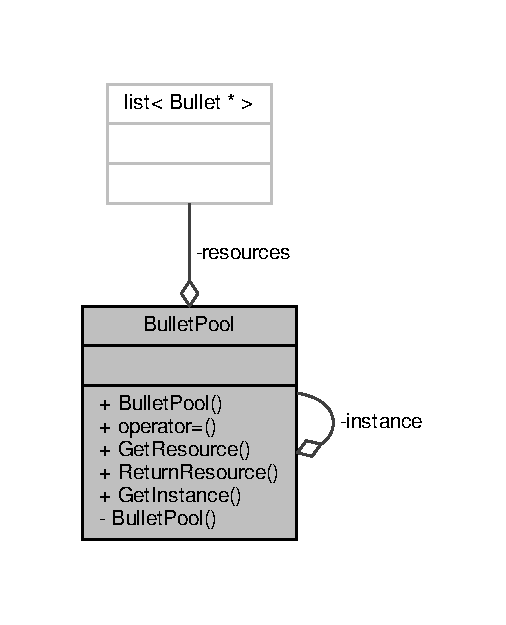
\includegraphics[width=243pt]{class_bullet_pool__coll__graph}
\end{center}
\end{figure}
\subsection*{Public Member Functions}
\begin{DoxyCompactItemize}
\item 
\hyperlink{class_bullet_pool_a13ca9f11d97405c0033612c389bfc06b}{Bullet\-Pool} (const \hyperlink{class_bullet_pool}{Bullet\-Pool} \&)=delete
\begin{DoxyCompactList}\small\item\em Delete copy constructor. \end{DoxyCompactList}\item 
\hyperlink{class_bullet_pool}{Bullet\-Pool} \& \hyperlink{class_bullet_pool_a808fcff0d6b8e4fa0b6954a0af689b79}{operator=} (const \hyperlink{class_bullet_pool}{Bullet\-Pool} \&)=delete
\begin{DoxyCompactList}\small\item\em Delete assignment operator. \end{DoxyCompactList}\item 
\hyperlink{class_bullet}{Bullet} $\ast$ \hyperlink{class_bullet_pool_ae80aa07016b9635d7637ea5796393d29}{Get\-Resource} ()
\begin{DoxyCompactList}\small\item\em Gets the resource. \end{DoxyCompactList}\item 
void \hyperlink{class_bullet_pool_aa821f65e3b2a2845471ba094a683560d}{Return\-Resource} (\hyperlink{class_bullet}{Bullet} $\ast$object)
\begin{DoxyCompactList}\small\item\em Returns a resource. \end{DoxyCompactList}\end{DoxyCompactItemize}
\subsection*{Static Public Member Functions}
\begin{DoxyCompactItemize}
\item 
static \hyperlink{class_bullet_pool}{Bullet\-Pool} $\ast$ \hyperlink{class_bullet_pool_a47b62aed3b35862ba203a5d0647b8d1a}{Get\-Instance} ()
\begin{DoxyCompactList}\small\item\em Gets the instance. \end{DoxyCompactList}\end{DoxyCompactItemize}
\subsection*{Private Member Functions}
\begin{DoxyCompactItemize}
\item 
\hyperlink{class_bullet_pool_ae1984d57ec3240c837589db4d25939e6}{Bullet\-Pool} ()
\begin{DoxyCompactList}\small\item\em Default constructor. \end{DoxyCompactList}\end{DoxyCompactItemize}
\subsection*{Private Attributes}
\begin{DoxyCompactItemize}
\item 
std\-::list$<$ \hyperlink{class_bullet}{Bullet} $\ast$ $>$ \hyperlink{class_bullet_pool_a1edef8514952653237ee829a197fd040}{resources}
\begin{DoxyCompactList}\small\item\em The resources. \end{DoxyCompactList}\end{DoxyCompactItemize}
\subsection*{Static Private Attributes}
\begin{DoxyCompactItemize}
\item 
static \hyperlink{class_bullet_pool}{Bullet\-Pool} $\ast$ \hyperlink{class_bullet_pool_aac55f9e917420391431f394836222baf}{instance} = 0
\begin{DoxyCompactList}\small\item\em The instance. \end{DoxyCompactList}\end{DoxyCompactItemize}


\subsection{Detailed Description}
A bullet pool. 



 

 

\subsection{Constructor \& Destructor Documentation}
\hypertarget{class_bullet_pool_a13ca9f11d97405c0033612c389bfc06b}{\index{Bullet\-Pool@{Bullet\-Pool}!Bullet\-Pool@{Bullet\-Pool}}
\index{Bullet\-Pool@{Bullet\-Pool}!BulletPool@{Bullet\-Pool}}
\subsubsection[{Bullet\-Pool}]{\setlength{\rightskip}{0pt plus 5cm}Bullet\-Pool\-::\-Bullet\-Pool (
\begin{DoxyParamCaption}
\item[{const {\bf Bullet\-Pool} \&}]{}
\end{DoxyParamCaption}
)\hspace{0.3cm}{\ttfamily [delete]}}}\label{class_bullet_pool_a13ca9f11d97405c0033612c389bfc06b}


Delete copy constructor. 



 

 \hypertarget{class_bullet_pool_ae1984d57ec3240c837589db4d25939e6}{\index{Bullet\-Pool@{Bullet\-Pool}!Bullet\-Pool@{Bullet\-Pool}}
\index{Bullet\-Pool@{Bullet\-Pool}!BulletPool@{Bullet\-Pool}}
\subsubsection[{Bullet\-Pool}]{\setlength{\rightskip}{0pt plus 5cm}Bullet\-Pool\-::\-Bullet\-Pool (
\begin{DoxyParamCaption}
{}
\end{DoxyParamCaption}
)\hspace{0.3cm}{\ttfamily [private]}}}\label{class_bullet_pool_ae1984d57ec3240c837589db4d25939e6}


Default constructor. 







 



\subsubsection*{}

\subsubsection*{Default constructor.  }

Referenced by Get\-Instance().


\begin{DoxyCode}
16 \{
17 
18 \}
\end{DoxyCode}


\subsection{Member Function Documentation}
\hypertarget{class_bullet_pool_a47b62aed3b35862ba203a5d0647b8d1a}{\index{Bullet\-Pool@{Bullet\-Pool}!Get\-Instance@{Get\-Instance}}
\index{Get\-Instance@{Get\-Instance}!BulletPool@{Bullet\-Pool}}
\subsubsection[{Get\-Instance}]{\setlength{\rightskip}{0pt plus 5cm}{\bf Bullet\-Pool} $\ast$ Bullet\-Pool\-::\-Get\-Instance (
\begin{DoxyParamCaption}
{}
\end{DoxyParamCaption}
)\hspace{0.3cm}{\ttfamily [static]}}}\label{class_bullet_pool_a47b62aed3b35862ba203a5d0647b8d1a}


Gets the instance. 



 

 

References Bullet\-Pool(), and instance.



Referenced by Player\-::\-Init().


\begin{DoxyCode}
27 \{
28     \textcolor{keywordflow}{if} (!\hyperlink{class_bullet_pool_aac55f9e917420391431f394836222baf}{instance})
29     \{
30         \hyperlink{class_bullet_pool_aac55f9e917420391431f394836222baf}{instance} = \textcolor{keyword}{new} \hyperlink{class_bullet_pool_ae1984d57ec3240c837589db4d25939e6}{BulletPool}();
31     \}
32     \textcolor{keywordflow}{return} \hyperlink{class_bullet_pool_aac55f9e917420391431f394836222baf}{instance};
33 \}
\end{DoxyCode}
\hypertarget{class_bullet_pool_ae80aa07016b9635d7637ea5796393d29}{\index{Bullet\-Pool@{Bullet\-Pool}!Get\-Resource@{Get\-Resource}}
\index{Get\-Resource@{Get\-Resource}!BulletPool@{Bullet\-Pool}}
\subsubsection[{Get\-Resource}]{\setlength{\rightskip}{0pt plus 5cm}{\bf Bullet} $\ast$ Bullet\-Pool\-::\-Get\-Resource (
\begin{DoxyParamCaption}
{}
\end{DoxyParamCaption}
)}}\label{class_bullet_pool_ae80aa07016b9635d7637ea5796393d29}


Gets the resource. 



 

 

References resources.



Referenced by Player\-::\-Shoot().


\begin{DoxyCode}
40 \{
41     \textcolor{keywordflow}{if} (\hyperlink{class_bullet_pool_a1edef8514952653237ee829a197fd040}{resources}.empty())
42     \{
43         \textcolor{keywordflow}{return} \textcolor{keyword}{new} \hyperlink{class_bullet}{Bullet}();
44     \}
45     \textcolor{keywordflow}{else}
46     \{
47         \hyperlink{class_bullet}{Bullet}* bullet = \hyperlink{class_bullet_pool_a1edef8514952653237ee829a197fd040}{resources}.front();
48         \hyperlink{class_bullet_pool_a1edef8514952653237ee829a197fd040}{resources}.pop\_front();
49         \textcolor{keywordflow}{return} bullet;
50     \}
51 \}
\end{DoxyCode}
\hypertarget{class_bullet_pool_a808fcff0d6b8e4fa0b6954a0af689b79}{\index{Bullet\-Pool@{Bullet\-Pool}!operator=@{operator=}}
\index{operator=@{operator=}!BulletPool@{Bullet\-Pool}}
\subsubsection[{operator=}]{\setlength{\rightskip}{0pt plus 5cm}{\bf Bullet\-Pool}\& Bullet\-Pool\-::operator= (
\begin{DoxyParamCaption}
\item[{const {\bf Bullet\-Pool} \&}]{}
\end{DoxyParamCaption}
)\hspace{0.3cm}{\ttfamily [delete]}}}\label{class_bullet_pool_a808fcff0d6b8e4fa0b6954a0af689b79}


Delete assignment operator. 



 

 \hypertarget{class_bullet_pool_aa821f65e3b2a2845471ba094a683560d}{\index{Bullet\-Pool@{Bullet\-Pool}!Return\-Resource@{Return\-Resource}}
\index{Return\-Resource@{Return\-Resource}!BulletPool@{Bullet\-Pool}}
\subsubsection[{Return\-Resource}]{\setlength{\rightskip}{0pt plus 5cm}void Bullet\-Pool\-::\-Return\-Resource (
\begin{DoxyParamCaption}
\item[{{\bf Bullet} $\ast$}]{object}
\end{DoxyParamCaption}
)}}\label{class_bullet_pool_aa821f65e3b2a2845471ba094a683560d}


Returns a resource. 

Resets the object and returns the resource back to the resources. 



 

 

References resources.



Referenced by Player\-::\-Shoot().


\begin{DoxyCode}
58 \{
59     \textcolor{keywordtype}{object}->Reset();
60     \hyperlink{class_bullet_pool_a1edef8514952653237ee829a197fd040}{resources}.push\_back(\textcolor{keywordtype}{object});
61 \}\end{DoxyCode}


\subsection{Member Data Documentation}
\hypertarget{class_bullet_pool_aac55f9e917420391431f394836222baf}{\index{Bullet\-Pool@{Bullet\-Pool}!instance@{instance}}
\index{instance@{instance}!BulletPool@{Bullet\-Pool}}
\subsubsection[{instance}]{\setlength{\rightskip}{0pt plus 5cm}{\bf Bullet\-Pool} $\ast$ Bullet\-Pool\-::instance = 0\hspace{0.3cm}{\ttfamily [static]}, {\ttfamily [private]}}}\label{class_bullet_pool_aac55f9e917420391431f394836222baf}


The instance. 



Referenced by Get\-Instance().

\hypertarget{class_bullet_pool_a1edef8514952653237ee829a197fd040}{\index{Bullet\-Pool@{Bullet\-Pool}!resources@{resources}}
\index{resources@{resources}!BulletPool@{Bullet\-Pool}}
\subsubsection[{resources}]{\setlength{\rightskip}{0pt plus 5cm}std\-::list$<${\bf Bullet}$\ast$$>$ Bullet\-Pool\-::resources\hspace{0.3cm}{\ttfamily [private]}}}\label{class_bullet_pool_a1edef8514952653237ee829a197fd040}


The resources. 



Referenced by Get\-Resource(), and Return\-Resource().



The documentation for this class was generated from the following files\-:\begin{DoxyCompactItemize}
\item 
\hyperlink{_bullet_pool_8h}{Bullet\-Pool.\-h}\item 
\hyperlink{_bullet_pool_8cpp}{Bullet\-Pool.\-cpp}\end{DoxyCompactItemize}

\hypertarget{class_camera}{\section{Camera Class Reference}
\label{class_camera}\index{Camera@{Camera}}
}


Top down camera that follows player  




{\ttfamily \#include $<$Camera.\-h$>$}



Collaboration diagram for Camera\-:
\nopagebreak
\begin{figure}[H]
\begin{center}
\leavevmode
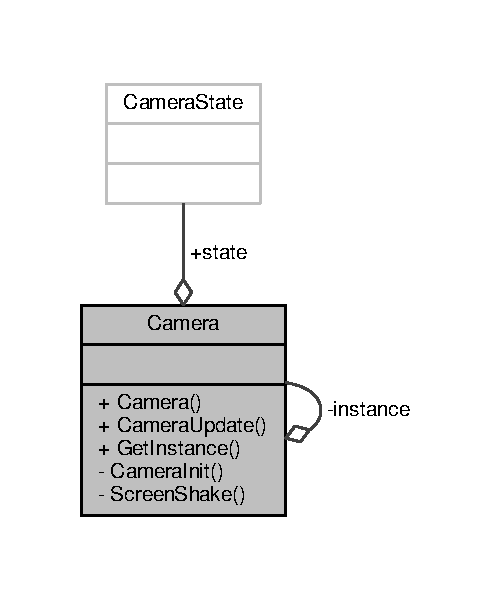
\includegraphics[width=238pt]{class_camera__coll__graph}
\end{center}
\end{figure}
\subsection*{Public Types}
\begin{DoxyCompactItemize}
\item 
enum \hyperlink{class_camera_a1ddf5d726e6c1d1d1c08d96d42c40236}{Camera\-State} \{ \\*
\hyperlink{class_camera_a1ddf5d726e6c1d1d1c08d96d42c40236abb7299ba8c5dcce883fe6987df129b1c}{normal}, 
\hyperlink{class_camera_a1ddf5d726e6c1d1d1c08d96d42c40236a9bb1793c9685b74a790ea306a7852179}{wave\-Shaking}, 
\hyperlink{class_camera_a1ddf5d726e6c1d1d1c08d96d42c40236a3a50c28c61cd1a7f837b32c54a65c92d}{big\-Wave\-Shaking}, 
\hyperlink{class_camera_a1ddf5d726e6c1d1d1c08d96d42c40236a0face68fe0053d79d3a1b03bd2a2645b}{shoot\-Shaking}, 
\\*
\hyperlink{class_camera_a1ddf5d726e6c1d1d1c08d96d42c40236a4d150a6fd04ef129c37e767d9087fa9f}{gameover}
 \}
\end{DoxyCompactItemize}
\subsection*{Public Member Functions}
\begin{DoxyCompactItemize}
\item 
\hyperlink{class_camera_a8dcadcfd314ecb49ac224a7e6d0bffde}{Camera} (irr\-::\-Irrlicht\-Device $\ast$device)
\begin{DoxyCompactList}\small\item\em Constructor. \end{DoxyCompactList}\item 
void \hyperlink{class_camera_a76e6167aa081ea6755d0bf588cd8cb73}{Camera\-Update} (f32 \hyperlink{_player_8cpp_adc988571147642cda93afbf89783f9c9}{frame\-Delta\-Time})
\begin{DoxyCompactList}\small\item\em Updates the camera position and target \end{DoxyCompactList}\end{DoxyCompactItemize}
\subsection*{Static Public Member Functions}
\begin{DoxyCompactItemize}
\item 
static \hyperlink{class_camera}{Camera} $\ast$ \hyperlink{class_camera_aae2256f0ee62dd982d92c09d9d00c8d5}{Get\-Instance} (Irrlicht\-Device $\ast$device)
\end{DoxyCompactItemize}
\subsection*{Public Attributes}
\begin{DoxyCompactItemize}
\item 
\hyperlink{class_camera_a1ddf5d726e6c1d1d1c08d96d42c40236}{Camera\-State} \hyperlink{class_camera_a87960570c2d28bd4471c5a74fc021cb5}{state}
\end{DoxyCompactItemize}
\subsection*{Private Member Functions}
\begin{DoxyCompactItemize}
\item 
void \hyperlink{class_camera_ab31de25cd3c79eb40dcb785fa280cda6}{Camera\-Init} ()
\begin{DoxyCompactList}\small\item\em Initialization of the \hyperlink{class_camera}{Camera} \end{DoxyCompactList}\item 
void \hyperlink{class_camera_a2a8b4c795eef0ecc8069f4ee9fe75fb3}{Screen\-Shake} (f32 frame\-Delta\-Tim, f32 intensity)
\end{DoxyCompactItemize}
\subsection*{Static Private Attributes}
\begin{DoxyCompactItemize}
\item 
static \hyperlink{class_camera}{Camera} $\ast$ \hyperlink{class_camera_af95982469bc5cdc45c48f464b9ff05b9}{instance} = 0
\begin{DoxyCompactList}\small\item\em Initializes the camera \end{DoxyCompactList}\end{DoxyCompactItemize}


\subsection{Detailed Description}
Top down camera that follows player 



 

 

\subsection{Member Enumeration Documentation}
\hypertarget{class_camera_a1ddf5d726e6c1d1d1c08d96d42c40236}{\index{Camera@{Camera}!Camera\-State@{Camera\-State}}
\index{Camera\-State@{Camera\-State}!Camera@{Camera}}
\subsubsection[{Camera\-State}]{\setlength{\rightskip}{0pt plus 5cm}enum {\bf Camera\-::\-Camera\-State}}}\label{class_camera_a1ddf5d726e6c1d1d1c08d96d42c40236}
\begin{Desc}
\item[Enumerator]\par
\begin{description}
\index{normal@{normal}!Camera@{Camera}}\index{Camera@{Camera}!normal@{normal}}\item[{\em 
\hypertarget{class_camera_a1ddf5d726e6c1d1d1c08d96d42c40236abb7299ba8c5dcce883fe6987df129b1c}{normal}\label{class_camera_a1ddf5d726e6c1d1d1c08d96d42c40236abb7299ba8c5dcce883fe6987df129b1c}
}]\index{wave\-Shaking@{wave\-Shaking}!Camera@{Camera}}\index{Camera@{Camera}!wave\-Shaking@{wave\-Shaking}}\item[{\em 
\hypertarget{class_camera_a1ddf5d726e6c1d1d1c08d96d42c40236a9bb1793c9685b74a790ea306a7852179}{wave\-Shaking}\label{class_camera_a1ddf5d726e6c1d1d1c08d96d42c40236a9bb1793c9685b74a790ea306a7852179}
}]\index{big\-Wave\-Shaking@{big\-Wave\-Shaking}!Camera@{Camera}}\index{Camera@{Camera}!big\-Wave\-Shaking@{big\-Wave\-Shaking}}\item[{\em 
\hypertarget{class_camera_a1ddf5d726e6c1d1d1c08d96d42c40236a3a50c28c61cd1a7f837b32c54a65c92d}{big\-Wave\-Shaking}\label{class_camera_a1ddf5d726e6c1d1d1c08d96d42c40236a3a50c28c61cd1a7f837b32c54a65c92d}
}]\index{shoot\-Shaking@{shoot\-Shaking}!Camera@{Camera}}\index{Camera@{Camera}!shoot\-Shaking@{shoot\-Shaking}}\item[{\em 
\hypertarget{class_camera_a1ddf5d726e6c1d1d1c08d96d42c40236a0face68fe0053d79d3a1b03bd2a2645b}{shoot\-Shaking}\label{class_camera_a1ddf5d726e6c1d1d1c08d96d42c40236a0face68fe0053d79d3a1b03bd2a2645b}
}]\index{gameover@{gameover}!Camera@{Camera}}\index{Camera@{Camera}!gameover@{gameover}}\item[{\em 
\hypertarget{class_camera_a1ddf5d726e6c1d1d1c08d96d42c40236a4d150a6fd04ef129c37e767d9087fa9f}{gameover}\label{class_camera_a1ddf5d726e6c1d1d1c08d96d42c40236a4d150a6fd04ef129c37e767d9087fa9f}
}]\end{description}
\end{Desc}

\begin{DoxyCode}
22     \{
23         \hyperlink{class_camera_a1ddf5d726e6c1d1d1c08d96d42c40236abb7299ba8c5dcce883fe6987df129b1c}{normal},
24         \hyperlink{class_camera_a1ddf5d726e6c1d1d1c08d96d42c40236a9bb1793c9685b74a790ea306a7852179}{waveShaking},
25         \hyperlink{class_camera_a1ddf5d726e6c1d1d1c08d96d42c40236a3a50c28c61cd1a7f837b32c54a65c92d}{bigWaveShaking},
26         \hyperlink{class_camera_a1ddf5d726e6c1d1d1c08d96d42c40236a0face68fe0053d79d3a1b03bd2a2645b}{shootShaking},
27         \hyperlink{class_camera_a1ddf5d726e6c1d1d1c08d96d42c40236a4d150a6fd04ef129c37e767d9087fa9f}{gameover}
28     \};
\end{DoxyCode}


\subsection{Constructor \& Destructor Documentation}
\hypertarget{class_camera_a8dcadcfd314ecb49ac224a7e6d0bffde}{\index{Camera@{Camera}!Camera@{Camera}}
\index{Camera@{Camera}!Camera@{Camera}}
\subsubsection[{Camera}]{\setlength{\rightskip}{0pt plus 5cm}Camera\-::\-Camera (
\begin{DoxyParamCaption}
\item[{irr\-::\-Irrlicht\-Device $\ast$}]{device}
\end{DoxyParamCaption}
)}}\label{class_camera_a8dcadcfd314ecb49ac224a7e6d0bffde}


Constructor. 



 

 

References \-\_\-sound\-Manager, camera\-I\-Device, camera\-Smgr, game\-\_\-, Game\-::\-Get\-Instance(), and Sound\-Manager\-::\-Get\-Instance().


\begin{DoxyCode}
67 \{
68     \hyperlink{_camera_8cpp_a30edcb606ee143928a2503208101c492}{cameraIDevice} = device;
69     \hyperlink{_camera_8cpp_a0cc2153984c669f761bff4f8bc18e79c}{cameraSmgr} = \hyperlink{_camera_8cpp_a30edcb606ee143928a2503208101c492}{cameraIDevice}->getSceneManager();
70     \hyperlink{_camera_8cpp_a73df19eb9d4f0b717dd7d767d601d60a}{game\_} = \hyperlink{_camera_8cpp_a73df19eb9d4f0b717dd7d767d601d60a}{game\_}->\hyperlink{class_game_aa989d3cee96d5ae093663bf62dea57e2}{GetInstance}();
71     \hyperlink{class_camera_ab31de25cd3c79eb40dcb785fa280cda6}{CameraInit}();
72     \hyperlink{_camera_8cpp_ad1177796ac002afe9773fee42f521b2b}{\_soundManager} = \hyperlink{_camera_8cpp_ad1177796ac002afe9773fee42f521b2b}{\_soundManager}->\hyperlink{class_sound_manager_a887480b38c9380c9fba23a2337df63be}{GetInstance}();
73 \}
\end{DoxyCode}


\subsection{Member Function Documentation}
\hypertarget{class_camera_ab31de25cd3c79eb40dcb785fa280cda6}{\index{Camera@{Camera}!Camera\-Init@{Camera\-Init}}
\index{Camera\-Init@{Camera\-Init}!Camera@{Camera}}
\subsubsection[{Camera\-Init}]{\setlength{\rightskip}{0pt plus 5cm}void Camera\-::\-Camera\-Init (
\begin{DoxyParamCaption}
{}
\end{DoxyParamCaption}
)\hspace{0.3cm}{\ttfamily [private]}}}\label{class_camera_ab31de25cd3c79eb40dcb785fa280cda6}


Initialization of the \hyperlink{class_camera}{Camera} 



 

 

References camera, camera\-Smgr, camera\-Start\-Position, camera\-Start\-Target, new\-Camera\-Position, and time.


\begin{DoxyCode}
80 \{
81     \hyperlink{_camera_8cpp_a8920f7ea5f818f312fd7462dd96a3a50}{camera} = \hyperlink{_camera_8cpp_a0cc2153984c669f761bff4f8bc18e79c}{cameraSmgr}->addCameraSceneNode();
82     \textcolor{keywordflow}{if} (\hyperlink{_camera_8cpp_a8920f7ea5f818f312fd7462dd96a3a50}{camera})
83     \{
84         \hyperlink{_camera_8cpp_a8920f7ea5f818f312fd7462dd96a3a50}{camera}->setPosition(\hyperlink{_camera_8cpp_a7c0be2a67c370806c3148499dbdc60c0}{cameraStartPosition});
85         \hyperlink{_camera_8cpp_a8920f7ea5f818f312fd7462dd96a3a50}{camera}->setTarget(\hyperlink{_camera_8cpp_a9b3909feb1d589415063db537ece08ad}{cameraStartTarget});
86         \hyperlink{_camera_8cpp_a251c0afd6da69664ff234daccd5db458}{newCameraPosition}.Y = 80; 
87     \}
88     \textcolor{comment}{//shakeTimer = maxTime;}
89     srand(\hyperlink{_player_8cpp_ab683520676b99a7bcc7a6299eb886247}{time}(0));
90     \hyperlink{class_camera_a87960570c2d28bd4471c5a74fc021cb5}{state} = \hyperlink{class_camera_a1ddf5d726e6c1d1d1c08d96d42c40236abb7299ba8c5dcce883fe6987df129b1c}{normal};
91 \}
\end{DoxyCode}
\hypertarget{class_camera_a76e6167aa081ea6755d0bf588cd8cb73}{\index{Camera@{Camera}!Camera\-Update@{Camera\-Update}}
\index{Camera\-Update@{Camera\-Update}!Camera@{Camera}}
\subsubsection[{Camera\-Update}]{\setlength{\rightskip}{0pt plus 5cm}void Camera\-::\-Camera\-Update (
\begin{DoxyParamCaption}
\item[{f32}]{frame\-Delta\-Time}
\end{DoxyParamCaption}
)}}\label{class_camera_a76e6167aa081ea6755d0bf588cd8cb73}


Updates the camera position and target 

Update camera position relative to the player while game is playing and move camera to start pos when game is over 



 

 

References \-\_\-sound\-Manager, camera, camera\-Start\-Position, camera\-Start\-Target, E\-A\-R\-T\-H\-Q\-U\-A\-K\-E\-\_\-\-S\-O\-U\-N\-D, Player\-::get\-Player\-Object(), is\-Shaking, max\-Time\-Normal\-Shake, new\-Camera\-Position, player\-\_\-, Sound\-Manager\-::\-Play\-Sound(), shake\-Timer, shot\-Time\-Shake, and sound\-Playing.



Referenced by Game\-::\-Update().


\begin{DoxyCode}
140 \{
141 
142     \textcolor{keywordflow}{switch} (\hyperlink{class_camera_a87960570c2d28bd4471c5a74fc021cb5}{state})
143     \{
144     \textcolor{keywordflow}{case} \hyperlink{class_camera_a1ddf5d726e6c1d1d1c08d96d42c40236abb7299ba8c5dcce883fe6987df129b1c}{normal}:
145         \textcolor{keywordflow}{if} (\hyperlink{_camera_8cpp_a8920f7ea5f818f312fd7462dd96a3a50}{camera})
146         \{
147             \hyperlink{_camera_8cpp_a251c0afd6da69664ff234daccd5db458}{newCameraPosition}.X = \hyperlink{_camera_8cpp_a9aee5bc0df47d284a38a6b4da40a28a8}{player\_}->
      \hyperlink{class_player_a2914f817c2fe9b34984e6d90e8d5322f}{getPlayerObject}()->getPosition().X;
148             \hyperlink{_camera_8cpp_a251c0afd6da69664ff234daccd5db458}{newCameraPosition}.Z = \hyperlink{_camera_8cpp_a9aee5bc0df47d284a38a6b4da40a28a8}{player\_}->
      \hyperlink{class_player_a2914f817c2fe9b34984e6d90e8d5322f}{getPlayerObject}()->getPosition().Z;
149             \hyperlink{_camera_8cpp_a8920f7ea5f818f312fd7462dd96a3a50}{camera}->setPosition(\hyperlink{_camera_8cpp_a251c0afd6da69664ff234daccd5db458}{newCameraPosition});
150             \hyperlink{_camera_8cpp_a8920f7ea5f818f312fd7462dd96a3a50}{camera}->setTarget(\hyperlink{_camera_8cpp_a9aee5bc0df47d284a38a6b4da40a28a8}{player\_}->\hyperlink{class_player_a2914f817c2fe9b34984e6d90e8d5322f}{getPlayerObject}()->getPosition());
151         \}
152         \hyperlink{_camera_8cpp_a6b7c8d48813d1dd4aac53ba41d2b1981}{soundPlaying} = \textcolor{keyword}{false};
153         \hyperlink{_camera_8cpp_a45e54b24c28f7f9f93771bbc7fc65fe0}{isShaking} = \textcolor{keyword}{false};
154         \textcolor{keywordflow}{break};
155     \textcolor{keywordflow}{case} \hyperlink{class_camera_a1ddf5d726e6c1d1d1c08d96d42c40236a9bb1793c9685b74a790ea306a7852179}{waveShaking}:
156         \textcolor{keywordflow}{if} (!\hyperlink{_camera_8cpp_a45e54b24c28f7f9f93771bbc7fc65fe0}{isShaking}) 
157         \{
158             \hyperlink{_camera_8cpp_a45e54b24c28f7f9f93771bbc7fc65fe0}{isShaking} = \textcolor{keyword}{true};
159             \hyperlink{_camera_8cpp_a06666e09f3081c828a90b1f36b5a6a20}{shakeTimer} = \hyperlink{_camera_8cpp_a619c0eb0387294c24a31b7db33b7794c}{maxTimeNormalShake};
160         \}
161         \hyperlink{class_camera_a2a8b4c795eef0ecc8069f4ee9fe75fb3}{ScreenShake}(\hyperlink{_player_8cpp_adc988571147642cda93afbf89783f9c9}{frameDeltaTime}, 0.4);
162         \textcolor{keywordflow}{if} (!\hyperlink{_camera_8cpp_a6b7c8d48813d1dd4aac53ba41d2b1981}{soundPlaying})
163         \{
164             \hyperlink{_camera_8cpp_a6b7c8d48813d1dd4aac53ba41d2b1981}{soundPlaying} = \textcolor{keyword}{true};
165             \hyperlink{_camera_8cpp_ad1177796ac002afe9773fee42f521b2b}{\_soundManager}->\hyperlink{class_sound_manager_a81e8f88fe549f6767d3552f12c28ecbc}{PlaySound}(\hyperlink{_camera_8cpp_abd32b9b9e58b56300d17f56603d2258f}{EARTHQUAKE\_SOUND}, \textcolor{keyword}{false});
166         \}
167         \textcolor{keywordflow}{break};
168     \textcolor{keywordflow}{case} \hyperlink{class_camera_a1ddf5d726e6c1d1d1c08d96d42c40236a3a50c28c61cd1a7f837b32c54a65c92d}{bigWaveShaking}:
169         \textcolor{keywordflow}{if} (!\hyperlink{_camera_8cpp_a45e54b24c28f7f9f93771bbc7fc65fe0}{isShaking})
170         \{
171             \hyperlink{_camera_8cpp_a45e54b24c28f7f9f93771bbc7fc65fe0}{isShaking} = \textcolor{keyword}{true};
172             \hyperlink{_camera_8cpp_a06666e09f3081c828a90b1f36b5a6a20}{shakeTimer} = \hyperlink{_camera_8cpp_a619c0eb0387294c24a31b7db33b7794c}{maxTimeNormalShake};
173         \}
174         \hyperlink{class_camera_a2a8b4c795eef0ecc8069f4ee9fe75fb3}{ScreenShake}(\hyperlink{_player_8cpp_adc988571147642cda93afbf89783f9c9}{frameDeltaTime}, 0.5);
175         \textcolor{keywordflow}{if} (!\hyperlink{_camera_8cpp_a6b7c8d48813d1dd4aac53ba41d2b1981}{soundPlaying})
176         \{
177             \hyperlink{_camera_8cpp_a6b7c8d48813d1dd4aac53ba41d2b1981}{soundPlaying} = \textcolor{keyword}{true};
178             \hyperlink{_camera_8cpp_ad1177796ac002afe9773fee42f521b2b}{\_soundManager}->\hyperlink{class_sound_manager_a81e8f88fe549f6767d3552f12c28ecbc}{PlaySound}(\hyperlink{_camera_8cpp_abd32b9b9e58b56300d17f56603d2258f}{EARTHQUAKE\_SOUND}, \textcolor{keyword}{false});
179         \}
180         \textcolor{keywordflow}{break};
181     \textcolor{keywordflow}{case} \hyperlink{class_camera_a1ddf5d726e6c1d1d1c08d96d42c40236a0face68fe0053d79d3a1b03bd2a2645b}{shootShaking}:
182         \textcolor{keywordflow}{if} (!\hyperlink{_camera_8cpp_a45e54b24c28f7f9f93771bbc7fc65fe0}{isShaking})
183         \{
184             \hyperlink{_camera_8cpp_a45e54b24c28f7f9f93771bbc7fc65fe0}{isShaking} = \textcolor{keyword}{true};
185             \hyperlink{_camera_8cpp_a06666e09f3081c828a90b1f36b5a6a20}{shakeTimer} = \hyperlink{_camera_8cpp_a5de58f108d9c49965afcc955ca60cf3a}{shotTimeShake};
186         \}
187         \hyperlink{class_camera_a2a8b4c795eef0ecc8069f4ee9fe75fb3}{ScreenShake}(\hyperlink{_player_8cpp_adc988571147642cda93afbf89783f9c9}{frameDeltaTime}, 2);
188         \textcolor{keywordflow}{break};
189     \textcolor{keywordflow}{case} \hyperlink{class_camera_a1ddf5d726e6c1d1d1c08d96d42c40236a4d150a6fd04ef129c37e767d9087fa9f}{gameover}:
190         \hyperlink{_camera_8cpp_a8920f7ea5f818f312fd7462dd96a3a50}{camera}->setPosition(\hyperlink{_camera_8cpp_a7c0be2a67c370806c3148499dbdc60c0}{cameraStartPosition});
191         \hyperlink{_camera_8cpp_a8920f7ea5f818f312fd7462dd96a3a50}{camera}->setTarget(\hyperlink{_camera_8cpp_a9b3909feb1d589415063db537ece08ad}{cameraStartTarget});
192         \textcolor{keywordflow}{break};
193     \}
194 \}
\end{DoxyCode}
\hypertarget{class_camera_aae2256f0ee62dd982d92c09d9d00c8d5}{\index{Camera@{Camera}!Get\-Instance@{Get\-Instance}}
\index{Get\-Instance@{Get\-Instance}!Camera@{Camera}}
\subsubsection[{Get\-Instance}]{\setlength{\rightskip}{0pt plus 5cm}{\bf Camera} $\ast$ Camera\-::\-Get\-Instance (
\begin{DoxyParamCaption}
\item[{Irrlicht\-Device $\ast$}]{device}
\end{DoxyParamCaption}
)\hspace{0.3cm}{\ttfamily [static]}}}\label{class_camera_aae2256f0ee62dd982d92c09d9d00c8d5}


Referenced by Enemy\-Spawner\-::\-Enemy\-Spawner(), Player\-::\-Init(), and Game\-::\-Start().


\begin{DoxyCode}
58 \{
59     \textcolor{keywordflow}{if} (!\hyperlink{class_camera_af95982469bc5cdc45c48f464b9ff05b9}{instance})
60     \{
61         \hyperlink{class_camera_af95982469bc5cdc45c48f464b9ff05b9}{instance} = \textcolor{keyword}{new} \hyperlink{class_camera_a8dcadcfd314ecb49ac224a7e6d0bffde}{Camera}(device);
62     \}
63     \textcolor{keywordflow}{return} \hyperlink{class_camera_af95982469bc5cdc45c48f464b9ff05b9}{instance};
64 \}
\end{DoxyCode}
\hypertarget{class_camera_a2a8b4c795eef0ecc8069f4ee9fe75fb3}{\index{Camera@{Camera}!Screen\-Shake@{Screen\-Shake}}
\index{Screen\-Shake@{Screen\-Shake}!Camera@{Camera}}
\subsubsection[{Screen\-Shake}]{\setlength{\rightskip}{0pt plus 5cm}void Camera\-::\-Screen\-Shake (
\begin{DoxyParamCaption}
\item[{f32}]{frame\-Delta\-Tim, }
\item[{f32}]{intensity}
\end{DoxyParamCaption}
)\hspace{0.3cm}{\ttfamily [private]}}}\label{class_camera_a2a8b4c795eef0ecc8069f4ee9fe75fb3}


References camera, frame\-Delta\-Time, Player\-::get\-Cam\-Follow\-Object(), Player\-::get\-Player\-Object(), new\-Camera\-Position, player\-\_\-, reset\-Time, and shake\-Timer.


\begin{DoxyCode}
94 \{
95     \textcolor{keywordflow}{if} (\hyperlink{_camera_8cpp_a06666e09f3081c828a90b1f36b5a6a20}{shakeTimer} > 0)
96     \{
97         \hyperlink{_camera_8cpp_a06666e09f3081c828a90b1f36b5a6a20}{shakeTimer} -= \hyperlink{_player_8cpp_adc988571147642cda93afbf89783f9c9}{frameDeltaTime};
98         \hyperlink{_camera_8cpp_a8652745f30900067bef50ae0b81d7141}{resetTime} += \hyperlink{_player_8cpp_adc988571147642cda93afbf89783f9c9}{frameDeltaTime};
99         
100 
101         \textcolor{keyword}{const} f32 dur = 0.6;
102         
103         vector3df playerPos = \hyperlink{_camera_8cpp_a9aee5bc0df47d284a38a6b4da40a28a8}{player\_}->\hyperlink{class_player_a2914f817c2fe9b34984e6d90e8d5322f}{getPlayerObject}()->getPosition();
104         vector3df randomVec = vector3df(playerPos.X + rand() % 2 * intensity, playerPos.Y, playerPos.Z + 
      rand() % 2 * intensity);
105         
106         \textcolor{keywordflow}{if} (\hyperlink{_camera_8cpp_a8652745f30900067bef50ae0b81d7141}{resetTime} <= dur) 
107         \{
108             \hyperlink{_camera_8cpp_a9aee5bc0df47d284a38a6b4da40a28a8}{player\_}->\hyperlink{class_player_ad41c9997bb4efcb41d8a82bf5b14c019}{getCamFollowObject}()->setPosition(randomVec);
109             \hyperlink{_camera_8cpp_a8920f7ea5f818f312fd7462dd96a3a50}{camera}->setTarget(\hyperlink{_camera_8cpp_a9aee5bc0df47d284a38a6b4da40a28a8}{player\_}->\hyperlink{class_player_ad41c9997bb4efcb41d8a82bf5b14c019}{getCamFollowObject}()->getPosition());
110             \hyperlink{_camera_8cpp_a251c0afd6da69664ff234daccd5db458}{newCameraPosition}.X = \hyperlink{_camera_8cpp_a9aee5bc0df47d284a38a6b4da40a28a8}{player\_}->
      \hyperlink{class_player_ad41c9997bb4efcb41d8a82bf5b14c019}{getCamFollowObject}()->getPosition().X;
111             \hyperlink{_camera_8cpp_a251c0afd6da69664ff234daccd5db458}{newCameraPosition}.Z = \hyperlink{_camera_8cpp_a9aee5bc0df47d284a38a6b4da40a28a8}{player\_}->
      \hyperlink{class_player_ad41c9997bb4efcb41d8a82bf5b14c019}{getCamFollowObject}()->getPosition().Z;
112             \hyperlink{_camera_8cpp_a8920f7ea5f818f312fd7462dd96a3a50}{camera}->setPosition(\hyperlink{_camera_8cpp_a251c0afd6da69664ff234daccd5db458}{newCameraPosition});
113         \}
114         \textcolor{keywordflow}{if} (\hyperlink{_camera_8cpp_a8652745f30900067bef50ae0b81d7141}{resetTime} > dur) 
115         \{
116             \hyperlink{_camera_8cpp_a9aee5bc0df47d284a38a6b4da40a28a8}{player\_}->\hyperlink{class_player_ad41c9997bb4efcb41d8a82bf5b14c019}{getCamFollowObject}()->setPosition(randomVec);
117             \hyperlink{_camera_8cpp_a8920f7ea5f818f312fd7462dd96a3a50}{camera}->setTarget(\hyperlink{_camera_8cpp_a9aee5bc0df47d284a38a6b4da40a28a8}{player\_}->\hyperlink{class_player_ad41c9997bb4efcb41d8a82bf5b14c019}{getCamFollowObject}()->getPosition());
118             \hyperlink{_camera_8cpp_a251c0afd6da69664ff234daccd5db458}{newCameraPosition}.X = \hyperlink{_camera_8cpp_a9aee5bc0df47d284a38a6b4da40a28a8}{player\_}->
      \hyperlink{class_player_ad41c9997bb4efcb41d8a82bf5b14c019}{getCamFollowObject}()->getPosition().X;
119             \hyperlink{_camera_8cpp_a251c0afd6da69664ff234daccd5db458}{newCameraPosition}.Z = \hyperlink{_camera_8cpp_a9aee5bc0df47d284a38a6b4da40a28a8}{player\_}->
      \hyperlink{class_player_ad41c9997bb4efcb41d8a82bf5b14c019}{getCamFollowObject}()->getPosition().Z;
120             \hyperlink{_camera_8cpp_a8920f7ea5f818f312fd7462dd96a3a50}{camera}->setPosition(\hyperlink{_camera_8cpp_a251c0afd6da69664ff234daccd5db458}{newCameraPosition});
121         \}
122         \textcolor{keywordflow}{if} (\hyperlink{_camera_8cpp_a8652745f30900067bef50ae0b81d7141}{resetTime} > dur * 2)
123         \{
124             \hyperlink{_camera_8cpp_a8652745f30900067bef50ae0b81d7141}{resetTime} = 0;
125         \}
126     \}
127     \textcolor{keywordflow}{else} 
128     \{
129         \textcolor{comment}{//shakeTimer = maxTime;}
130         \hyperlink{class_camera_a87960570c2d28bd4471c5a74fc021cb5}{state} = \hyperlink{class_camera_a1ddf5d726e6c1d1d1c08d96d42c40236abb7299ba8c5dcce883fe6987df129b1c}{normal};
131     \}
132 \}
\end{DoxyCode}


\subsection{Member Data Documentation}
\hypertarget{class_camera_af95982469bc5cdc45c48f464b9ff05b9}{\index{Camera@{Camera}!instance@{instance}}
\index{instance@{instance}!Camera@{Camera}}
\subsubsection[{instance}]{\setlength{\rightskip}{0pt plus 5cm}{\bf Camera} $\ast$ Camera\-::instance = 0\hspace{0.3cm}{\ttfamily [static]}, {\ttfamily [private]}}}\label{class_camera_af95982469bc5cdc45c48f464b9ff05b9}


Initializes the camera 

Constructor. 



 

 \hypertarget{class_camera_a87960570c2d28bd4471c5a74fc021cb5}{\index{Camera@{Camera}!state@{state}}
\index{state@{state}!Camera@{Camera}}
\subsubsection[{state}]{\setlength{\rightskip}{0pt plus 5cm}{\bf Camera\-State} Camera\-::state}}\label{class_camera_a87960570c2d28bd4471c5a74fc021cb5}


Referenced by Enemy\-Spawner\-::\-Next\-Wave(), Game\-::\-Set\-Is\-Game\-Over(), and Player\-::\-Shoot().



The documentation for this class was generated from the following files\-:\begin{DoxyCompactItemize}
\item 
\hyperlink{_camera_8h}{Camera.\-h}\item 
\hyperlink{_camera_8cpp}{Camera.\-cpp}\end{DoxyCompactItemize}

\hypertarget{struct_catch_1_1_matchers_1_1_std_string_1_1_cased_string}{\section{Catch\-:\-:Matchers\-:\-:Std\-String\-:\-:Cased\-String Struct Reference}
\label{struct_catch_1_1_matchers_1_1_std_string_1_1_cased_string}\index{Catch\-::\-Matchers\-::\-Std\-String\-::\-Cased\-String@{Catch\-::\-Matchers\-::\-Std\-String\-::\-Cased\-String}}
}


{\ttfamily \#include $<$catch.\-hpp$>$}



Collaboration diagram for Catch\-:\-:Matchers\-:\-:Std\-String\-:\-:Cased\-String\-:
\nopagebreak
\begin{figure}[H]
\begin{center}
\leavevmode
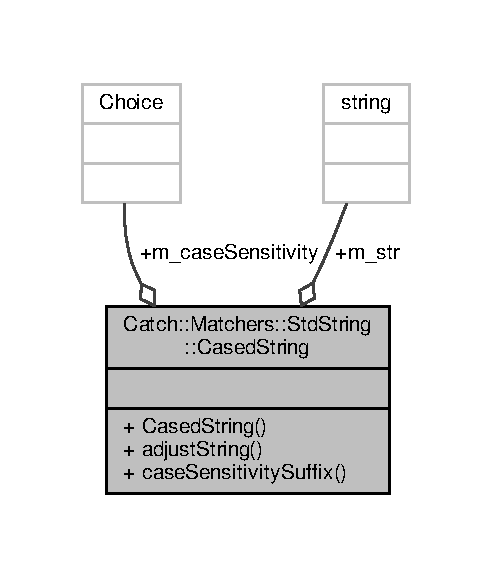
\includegraphics[width=236pt]{struct_catch_1_1_matchers_1_1_std_string_1_1_cased_string__coll__graph}
\end{center}
\end{figure}
\subsection*{Public Member Functions}
\begin{DoxyCompactItemize}
\item 
\hyperlink{struct_catch_1_1_matchers_1_1_std_string_1_1_cased_string_aa88bbc5acd2bff22351d8d4b1816b561}{Cased\-String} (std\-::string const \&str, \hyperlink{struct_catch_1_1_case_sensitive_aad49d3aee2d97066642fffa919685c6a}{Case\-Sensitive\-::\-Choice} case\-Sensitivity)
\item 
std\-::string \hyperlink{struct_catch_1_1_matchers_1_1_std_string_1_1_cased_string_a0ff84e194426c8f4bca0660b9180d20d}{adjust\-String} (std\-::string const \&str) const 
\item 
std\-::string \hyperlink{struct_catch_1_1_matchers_1_1_std_string_1_1_cased_string_a1113c80dd02967032a99290bdcd1b590}{case\-Sensitivity\-Suffix} () const 
\end{DoxyCompactItemize}
\subsection*{Public Attributes}
\begin{DoxyCompactItemize}
\item 
\hyperlink{struct_catch_1_1_case_sensitive_aad49d3aee2d97066642fffa919685c6a}{Case\-Sensitive\-::\-Choice} \hyperlink{struct_catch_1_1_matchers_1_1_std_string_1_1_cased_string_ae1c2864c986941536a6e94cca0528f92}{m\-\_\-case\-Sensitivity}
\item 
std\-::string \hyperlink{struct_catch_1_1_matchers_1_1_std_string_1_1_cased_string_ad05dbc99aba3c3c386d6b856b213f911}{m\-\_\-str}
\end{DoxyCompactItemize}


\subsection{Constructor \& Destructor Documentation}
\hypertarget{struct_catch_1_1_matchers_1_1_std_string_1_1_cased_string_aa88bbc5acd2bff22351d8d4b1816b561}{\index{Catch\-::\-Matchers\-::\-Std\-String\-::\-Cased\-String@{Catch\-::\-Matchers\-::\-Std\-String\-::\-Cased\-String}!Cased\-String@{Cased\-String}}
\index{Cased\-String@{Cased\-String}!Catch::Matchers::StdString::CasedString@{Catch\-::\-Matchers\-::\-Std\-String\-::\-Cased\-String}}
\subsubsection[{Cased\-String}]{\setlength{\rightskip}{0pt plus 5cm}Catch\-::\-Matchers\-::\-Std\-String\-::\-Cased\-String\-::\-Cased\-String (
\begin{DoxyParamCaption}
\item[{std\-::string const \&}]{str, }
\item[{{\bf Case\-Sensitive\-::\-Choice}}]{case\-Sensitivity}
\end{DoxyParamCaption}
)}}\label{struct_catch_1_1_matchers_1_1_std_string_1_1_cased_string_aa88bbc5acd2bff22351d8d4b1816b561}


\subsection{Member Function Documentation}
\hypertarget{struct_catch_1_1_matchers_1_1_std_string_1_1_cased_string_a0ff84e194426c8f4bca0660b9180d20d}{\index{Catch\-::\-Matchers\-::\-Std\-String\-::\-Cased\-String@{Catch\-::\-Matchers\-::\-Std\-String\-::\-Cased\-String}!adjust\-String@{adjust\-String}}
\index{adjust\-String@{adjust\-String}!Catch::Matchers::StdString::CasedString@{Catch\-::\-Matchers\-::\-Std\-String\-::\-Cased\-String}}
\subsubsection[{adjust\-String}]{\setlength{\rightskip}{0pt plus 5cm}std\-::string Catch\-::\-Matchers\-::\-Std\-String\-::\-Cased\-String\-::adjust\-String (
\begin{DoxyParamCaption}
\item[{std\-::string const \&}]{str}
\end{DoxyParamCaption}
) const}}\label{struct_catch_1_1_matchers_1_1_std_string_1_1_cased_string_a0ff84e194426c8f4bca0660b9180d20d}
\hypertarget{struct_catch_1_1_matchers_1_1_std_string_1_1_cased_string_a1113c80dd02967032a99290bdcd1b590}{\index{Catch\-::\-Matchers\-::\-Std\-String\-::\-Cased\-String@{Catch\-::\-Matchers\-::\-Std\-String\-::\-Cased\-String}!case\-Sensitivity\-Suffix@{case\-Sensitivity\-Suffix}}
\index{case\-Sensitivity\-Suffix@{case\-Sensitivity\-Suffix}!Catch::Matchers::StdString::CasedString@{Catch\-::\-Matchers\-::\-Std\-String\-::\-Cased\-String}}
\subsubsection[{case\-Sensitivity\-Suffix}]{\setlength{\rightskip}{0pt plus 5cm}std\-::string Catch\-::\-Matchers\-::\-Std\-String\-::\-Cased\-String\-::case\-Sensitivity\-Suffix (
\begin{DoxyParamCaption}
{}
\end{DoxyParamCaption}
) const}}\label{struct_catch_1_1_matchers_1_1_std_string_1_1_cased_string_a1113c80dd02967032a99290bdcd1b590}


\subsection{Member Data Documentation}
\hypertarget{struct_catch_1_1_matchers_1_1_std_string_1_1_cased_string_ae1c2864c986941536a6e94cca0528f92}{\index{Catch\-::\-Matchers\-::\-Std\-String\-::\-Cased\-String@{Catch\-::\-Matchers\-::\-Std\-String\-::\-Cased\-String}!m\-\_\-case\-Sensitivity@{m\-\_\-case\-Sensitivity}}
\index{m\-\_\-case\-Sensitivity@{m\-\_\-case\-Sensitivity}!Catch::Matchers::StdString::CasedString@{Catch\-::\-Matchers\-::\-Std\-String\-::\-Cased\-String}}
\subsubsection[{m\-\_\-case\-Sensitivity}]{\setlength{\rightskip}{0pt plus 5cm}{\bf Case\-Sensitive\-::\-Choice} Catch\-::\-Matchers\-::\-Std\-String\-::\-Cased\-String\-::m\-\_\-case\-Sensitivity}}\label{struct_catch_1_1_matchers_1_1_std_string_1_1_cased_string_ae1c2864c986941536a6e94cca0528f92}
\hypertarget{struct_catch_1_1_matchers_1_1_std_string_1_1_cased_string_ad05dbc99aba3c3c386d6b856b213f911}{\index{Catch\-::\-Matchers\-::\-Std\-String\-::\-Cased\-String@{Catch\-::\-Matchers\-::\-Std\-String\-::\-Cased\-String}!m\-\_\-str@{m\-\_\-str}}
\index{m\-\_\-str@{m\-\_\-str}!Catch::Matchers::StdString::CasedString@{Catch\-::\-Matchers\-::\-Std\-String\-::\-Cased\-String}}
\subsubsection[{m\-\_\-str}]{\setlength{\rightskip}{0pt plus 5cm}std\-::string Catch\-::\-Matchers\-::\-Std\-String\-::\-Cased\-String\-::m\-\_\-str}}\label{struct_catch_1_1_matchers_1_1_std_string_1_1_cased_string_ad05dbc99aba3c3c386d6b856b213f911}


The documentation for this struct was generated from the following file\-:\begin{DoxyCompactItemize}
\item 
\hyperlink{catch_8hpp}{catch.\-hpp}\end{DoxyCompactItemize}

\hypertarget{struct_catch_1_1_case_sensitive}{\section{Catch\-:\-:Case\-Sensitive Struct Reference}
\label{struct_catch_1_1_case_sensitive}\index{Catch\-::\-Case\-Sensitive@{Catch\-::\-Case\-Sensitive}}
}


{\ttfamily \#include $<$catch.\-hpp$>$}



Collaboration diagram for Catch\-:\-:Case\-Sensitive\-:
\nopagebreak
\begin{figure}[H]
\begin{center}
\leavevmode
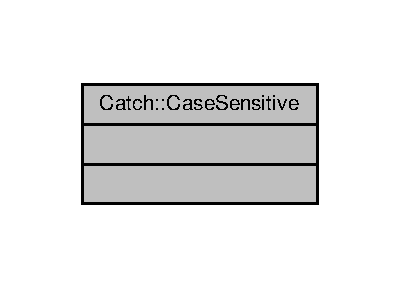
\includegraphics[width=192pt]{struct_catch_1_1_case_sensitive__coll__graph}
\end{center}
\end{figure}
\subsection*{Public Types}
\begin{DoxyCompactItemize}
\item 
enum \hyperlink{struct_catch_1_1_case_sensitive_aad49d3aee2d97066642fffa919685c6a}{Choice} \{ \hyperlink{struct_catch_1_1_case_sensitive_aad49d3aee2d97066642fffa919685c6aa7c5550b69ec3c502e6f609b67f9613c6}{Yes}, 
\hyperlink{struct_catch_1_1_case_sensitive_aad49d3aee2d97066642fffa919685c6aa4ffff8d29b481f0116abc37228cd53f6}{No}
 \}
\end{DoxyCompactItemize}


\subsection{Member Enumeration Documentation}
\hypertarget{struct_catch_1_1_case_sensitive_aad49d3aee2d97066642fffa919685c6a}{\index{Catch\-::\-Case\-Sensitive@{Catch\-::\-Case\-Sensitive}!Choice@{Choice}}
\index{Choice@{Choice}!Catch::CaseSensitive@{Catch\-::\-Case\-Sensitive}}
\subsubsection[{Choice}]{\setlength{\rightskip}{0pt plus 5cm}enum {\bf Catch\-::\-Case\-Sensitive\-::\-Choice}}}\label{struct_catch_1_1_case_sensitive_aad49d3aee2d97066642fffa919685c6a}
\begin{Desc}
\item[Enumerator]\par
\begin{description}
\index{Yes@{Yes}!Catch\-::\-Case\-Sensitive@{Catch\-::\-Case\-Sensitive}}\index{Catch\-::\-Case\-Sensitive@{Catch\-::\-Case\-Sensitive}!Yes@{Yes}}\item[{\em 
\hypertarget{struct_catch_1_1_case_sensitive_aad49d3aee2d97066642fffa919685c6aa7c5550b69ec3c502e6f609b67f9613c6}{Yes}\label{struct_catch_1_1_case_sensitive_aad49d3aee2d97066642fffa919685c6aa7c5550b69ec3c502e6f609b67f9613c6}
}]\index{No@{No}!Catch\-::\-Case\-Sensitive@{Catch\-::\-Case\-Sensitive}}\index{Catch\-::\-Case\-Sensitive@{Catch\-::\-Case\-Sensitive}!No@{No}}\item[{\em 
\hypertarget{struct_catch_1_1_case_sensitive_aad49d3aee2d97066642fffa919685c6aa4ffff8d29b481f0116abc37228cd53f6}{No}\label{struct_catch_1_1_case_sensitive_aad49d3aee2d97066642fffa919685c6aa4ffff8d29b481f0116abc37228cd53f6}
}]\end{description}
\end{Desc}

\begin{DoxyCode}
257                     \{
258             \hyperlink{struct_catch_1_1_case_sensitive_aad49d3aee2d97066642fffa919685c6aa7c5550b69ec3c502e6f609b67f9613c6}{Yes},
259             \hyperlink{struct_catch_1_1_case_sensitive_aad49d3aee2d97066642fffa919685c6aa4ffff8d29b481f0116abc37228cd53f6}{No}
260         \};
\end{DoxyCode}


The documentation for this struct was generated from the following file\-:\begin{DoxyCompactItemize}
\item 
\hyperlink{catch_8hpp}{catch.\-hpp}\end{DoxyCompactItemize}

\hypertarget{struct_catch__global__namespace__dummy}{\section{Catch\-\_\-global\-\_\-namespace\-\_\-dummy Struct Reference}
\label{struct_catch__global__namespace__dummy}\index{Catch\-\_\-global\-\_\-namespace\-\_\-dummy@{Catch\-\_\-global\-\_\-namespace\-\_\-dummy}}
}


{\ttfamily \#include $<$catch.\-hpp$>$}



Collaboration diagram for Catch\-\_\-global\-\_\-namespace\-\_\-dummy\-:
\nopagebreak
\begin{figure}[H]
\begin{center}
\leavevmode
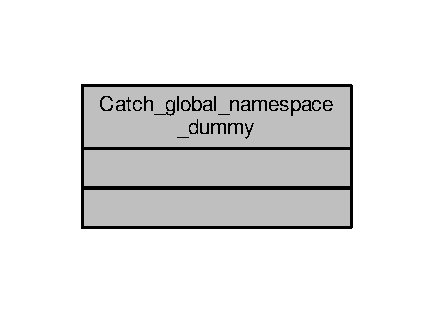
\includegraphics[width=208pt]{struct_catch__global__namespace__dummy__coll__graph}
\end{center}
\end{figure}


The documentation for this struct was generated from the following file\-:\begin{DoxyCompactItemize}
\item 
\hyperlink{catch_8hpp}{catch.\-hpp}\end{DoxyCompactItemize}

\hypertarget{class_collision}{}\section{Collision Class Reference}
\label{class_collision}\index{Collision@{Collision}}
\subsection*{Public Member Functions}
\begin{DoxyCompactItemize}
\item 
\mbox{\Hypertarget{class_collision_aa2fa3418899ac7948b31eb909dea6f04}\label{class_collision_aa2fa3418899ac7948b31eb909dea6f04}} 
bool {\bfseries Scene\+Node\+With\+Scene\+Node} (irr\+::scene\+::\+I\+Scene\+Node $\ast$t\+Box1, irr\+::scene\+::\+I\+Scene\+Node $\ast$t\+Box2)
\item 
\mbox{\Hypertarget{class_collision_a673528880f1ad75dab13a2107a3d2b7c}\label{class_collision_a673528880f1ad75dab13a2107a3d2b7c}} 
void {\bfseries Add\+Static\+To\+List} (irr\+::scene\+::\+I\+Scene\+Node $\ast$static\+Object)
\item 
\mbox{\Hypertarget{class_collision_a334467ec1c8b7889aa46016fcedb13f9}\label{class_collision_a334467ec1c8b7889aa46016fcedb13f9}} 
bool {\bfseries Collides\+With\+Static\+Objects} (irr\+::scene\+::\+I\+Scene\+Node $\ast$dynamic\+Object)
\end{DoxyCompactItemize}


The documentation for this class was generated from the following files\+:\begin{DoxyCompactItemize}
\item 
D\+:/\+Documenten/\+S\+T\+U\+D\+I\+E G\+D/\+Game Engine/\+Irrlicht project/kommandos/Collision.\+h\item 
D\+:/\+Documenten/\+S\+T\+U\+D\+I\+E G\+D/\+Game Engine/\+Irrlicht project/kommandos/Collision.\+cpp\end{DoxyCompactItemize}

\hypertarget{struct_catch_1_1_matchers_1_1_vector_1_1_contains_element_matcher}{\section{Catch\-:\-:Matchers\-:\-:Vector\-:\-:Contains\-Element\-Matcher$<$ T $>$ Struct Template Reference}
\label{struct_catch_1_1_matchers_1_1_vector_1_1_contains_element_matcher}\index{Catch\-::\-Matchers\-::\-Vector\-::\-Contains\-Element\-Matcher$<$ T $>$@{Catch\-::\-Matchers\-::\-Vector\-::\-Contains\-Element\-Matcher$<$ T $>$}}
}


{\ttfamily \#include $<$catch.\-hpp$>$}



Inheritance diagram for Catch\-:\-:Matchers\-:\-:Vector\-:\-:Contains\-Element\-Matcher$<$ T $>$\-:
\nopagebreak
\begin{figure}[H]
\begin{center}
\leavevmode
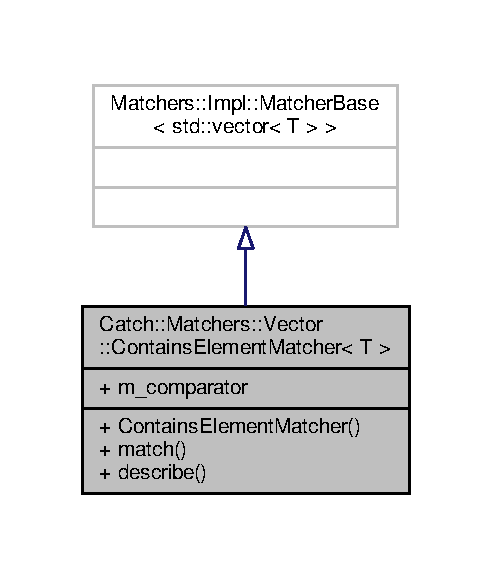
\includegraphics[width=236pt]{struct_catch_1_1_matchers_1_1_vector_1_1_contains_element_matcher__inherit__graph}
\end{center}
\end{figure}


Collaboration diagram for Catch\-:\-:Matchers\-:\-:Vector\-:\-:Contains\-Element\-Matcher$<$ T $>$\-:
\nopagebreak
\begin{figure}[H]
\begin{center}
\leavevmode
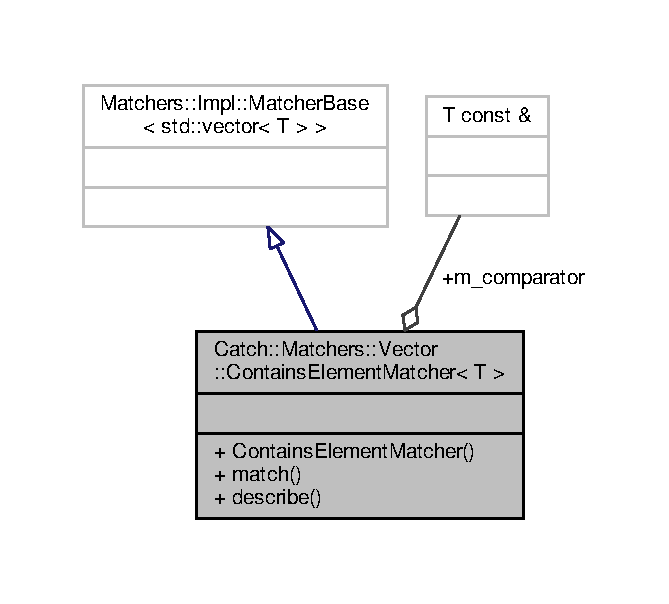
\includegraphics[width=321pt]{struct_catch_1_1_matchers_1_1_vector_1_1_contains_element_matcher__coll__graph}
\end{center}
\end{figure}
\subsection*{Public Member Functions}
\begin{DoxyCompactItemize}
\item 
\hyperlink{struct_catch_1_1_matchers_1_1_vector_1_1_contains_element_matcher_a6a05740b5d3f89fac8de84ac0cff7b93}{Contains\-Element\-Matcher} (T const \&comparator)
\item 
bool \hyperlink{struct_catch_1_1_matchers_1_1_vector_1_1_contains_element_matcher_a6a4be6e5642e267433d370649beb0fac}{match} (std\-::vector$<$ T $>$ const \&v) const override
\item 
std\-::string \hyperlink{struct_catch_1_1_matchers_1_1_vector_1_1_contains_element_matcher_aea3b674389a0afd82af6ba4b10f86ae6}{describe} () const override
\end{DoxyCompactItemize}
\subsection*{Public Attributes}
\begin{DoxyCompactItemize}
\item 
T const \& \hyperlink{struct_catch_1_1_matchers_1_1_vector_1_1_contains_element_matcher_ab7eada6c4bbce1d21b44773262f9cb23}{m\-\_\-comparator}
\end{DoxyCompactItemize}


\subsection{Constructor \& Destructor Documentation}
\hypertarget{struct_catch_1_1_matchers_1_1_vector_1_1_contains_element_matcher_a6a05740b5d3f89fac8de84ac0cff7b93}{\index{Catch\-::\-Matchers\-::\-Vector\-::\-Contains\-Element\-Matcher@{Catch\-::\-Matchers\-::\-Vector\-::\-Contains\-Element\-Matcher}!Contains\-Element\-Matcher@{Contains\-Element\-Matcher}}
\index{Contains\-Element\-Matcher@{Contains\-Element\-Matcher}!Catch::Matchers::Vector::ContainsElementMatcher@{Catch\-::\-Matchers\-::\-Vector\-::\-Contains\-Element\-Matcher}}
\subsubsection[{Contains\-Element\-Matcher}]{\setlength{\rightskip}{0pt plus 5cm}template$<$typename T $>$ {\bf Catch\-::\-Matchers\-::\-Vector\-::\-Contains\-Element\-Matcher}$<$ T $>$\-::{\bf Contains\-Element\-Matcher} (
\begin{DoxyParamCaption}
\item[{T const \&}]{comparator}
\end{DoxyParamCaption}
)\hspace{0.3cm}{\ttfamily [inline]}}}\label{struct_catch_1_1_matchers_1_1_vector_1_1_contains_element_matcher_a6a05740b5d3f89fac8de84ac0cff7b93}

\begin{DoxyCode}
2556 : \hyperlink{struct_catch_1_1_matchers_1_1_vector_1_1_contains_element_matcher_ab7eada6c4bbce1d21b44773262f9cb23}{m\_comparator}(comparator) \{\}
\end{DoxyCode}


\subsection{Member Function Documentation}
\hypertarget{struct_catch_1_1_matchers_1_1_vector_1_1_contains_element_matcher_aea3b674389a0afd82af6ba4b10f86ae6}{\index{Catch\-::\-Matchers\-::\-Vector\-::\-Contains\-Element\-Matcher@{Catch\-::\-Matchers\-::\-Vector\-::\-Contains\-Element\-Matcher}!describe@{describe}}
\index{describe@{describe}!Catch::Matchers::Vector::ContainsElementMatcher@{Catch\-::\-Matchers\-::\-Vector\-::\-Contains\-Element\-Matcher}}
\subsubsection[{describe}]{\setlength{\rightskip}{0pt plus 5cm}template$<$typename T $>$ std\-::string {\bf Catch\-::\-Matchers\-::\-Vector\-::\-Contains\-Element\-Matcher}$<$ T $>$\-::describe (
\begin{DoxyParamCaption}
{}
\end{DoxyParamCaption}
) const\hspace{0.3cm}{\ttfamily [inline]}, {\ttfamily [override]}}}\label{struct_catch_1_1_matchers_1_1_vector_1_1_contains_element_matcher_aea3b674389a0afd82af6ba4b10f86ae6}


References Catch\-::\-Detail\-::stringify().


\begin{DoxyCode}
2567                                                     \{
2568                     \textcolor{keywordflow}{return} \textcolor{stringliteral}{"Contains: "} + \hyperlink{namespace_catch_1_1_detail_af0ad48344ffd3f92f3568465248a9880}{::Catch::Detail::stringify}(
      \hyperlink{struct_catch_1_1_matchers_1_1_vector_1_1_contains_element_matcher_ab7eada6c4bbce1d21b44773262f9cb23}{m\_comparator});
2569                 \}
\end{DoxyCode}
\hypertarget{struct_catch_1_1_matchers_1_1_vector_1_1_contains_element_matcher_a6a4be6e5642e267433d370649beb0fac}{\index{Catch\-::\-Matchers\-::\-Vector\-::\-Contains\-Element\-Matcher@{Catch\-::\-Matchers\-::\-Vector\-::\-Contains\-Element\-Matcher}!match@{match}}
\index{match@{match}!Catch::Matchers::Vector::ContainsElementMatcher@{Catch\-::\-Matchers\-::\-Vector\-::\-Contains\-Element\-Matcher}}
\subsubsection[{match}]{\setlength{\rightskip}{0pt plus 5cm}template$<$typename T $>$ bool {\bf Catch\-::\-Matchers\-::\-Vector\-::\-Contains\-Element\-Matcher}$<$ T $>$\-::match (
\begin{DoxyParamCaption}
\item[{std\-::vector$<$ T $>$ const \&}]{v}
\end{DoxyParamCaption}
) const\hspace{0.3cm}{\ttfamily [inline]}, {\ttfamily [override]}}}\label{struct_catch_1_1_matchers_1_1_vector_1_1_contains_element_matcher_a6a4be6e5642e267433d370649beb0fac}

\begin{DoxyCode}
2558                                                                  \{
2559                     \textcolor{keywordflow}{for} (\textcolor{keyword}{auto} \textcolor{keyword}{const}& el : v) \{
2560                         \textcolor{keywordflow}{if} (el == \hyperlink{struct_catch_1_1_matchers_1_1_vector_1_1_contains_element_matcher_ab7eada6c4bbce1d21b44773262f9cb23}{m\_comparator}) \{
2561                             \textcolor{keywordflow}{return} \textcolor{keyword}{true};
2562                         \}
2563                     \}
2564                     \textcolor{keywordflow}{return} \textcolor{keyword}{false};
2565                 \}
\end{DoxyCode}


\subsection{Member Data Documentation}
\hypertarget{struct_catch_1_1_matchers_1_1_vector_1_1_contains_element_matcher_ab7eada6c4bbce1d21b44773262f9cb23}{\index{Catch\-::\-Matchers\-::\-Vector\-::\-Contains\-Element\-Matcher@{Catch\-::\-Matchers\-::\-Vector\-::\-Contains\-Element\-Matcher}!m\-\_\-comparator@{m\-\_\-comparator}}
\index{m\-\_\-comparator@{m\-\_\-comparator}!Catch::Matchers::Vector::ContainsElementMatcher@{Catch\-::\-Matchers\-::\-Vector\-::\-Contains\-Element\-Matcher}}
\subsubsection[{m\-\_\-comparator}]{\setlength{\rightskip}{0pt plus 5cm}template$<$typename T $>$ T const\& {\bf Catch\-::\-Matchers\-::\-Vector\-::\-Contains\-Element\-Matcher}$<$ T $>$\-::m\-\_\-comparator}}\label{struct_catch_1_1_matchers_1_1_vector_1_1_contains_element_matcher_ab7eada6c4bbce1d21b44773262f9cb23}


The documentation for this struct was generated from the following file\-:\begin{DoxyCompactItemize}
\item 
\hyperlink{catch_8hpp}{catch.\-hpp}\end{DoxyCompactItemize}

\hypertarget{struct_catch_1_1_matchers_1_1_std_string_1_1_contains_matcher}{\section{Catch\-:\-:Matchers\-:\-:Std\-String\-:\-:Contains\-Matcher Struct Reference}
\label{struct_catch_1_1_matchers_1_1_std_string_1_1_contains_matcher}\index{Catch\-::\-Matchers\-::\-Std\-String\-::\-Contains\-Matcher@{Catch\-::\-Matchers\-::\-Std\-String\-::\-Contains\-Matcher}}
}


{\ttfamily \#include $<$catch.\-hpp$>$}



Inheritance diagram for Catch\-:\-:Matchers\-:\-:Std\-String\-:\-:Contains\-Matcher\-:
\nopagebreak
\begin{figure}[H]
\begin{center}
\leavevmode
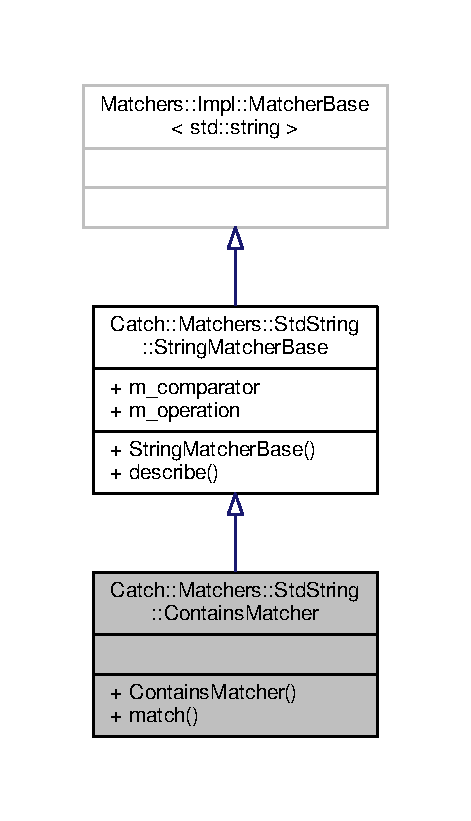
\includegraphics[width=226pt]{struct_catch_1_1_matchers_1_1_std_string_1_1_contains_matcher__inherit__graph}
\end{center}
\end{figure}


Collaboration diagram for Catch\-:\-:Matchers\-:\-:Std\-String\-:\-:Contains\-Matcher\-:
\nopagebreak
\begin{figure}[H]
\begin{center}
\leavevmode
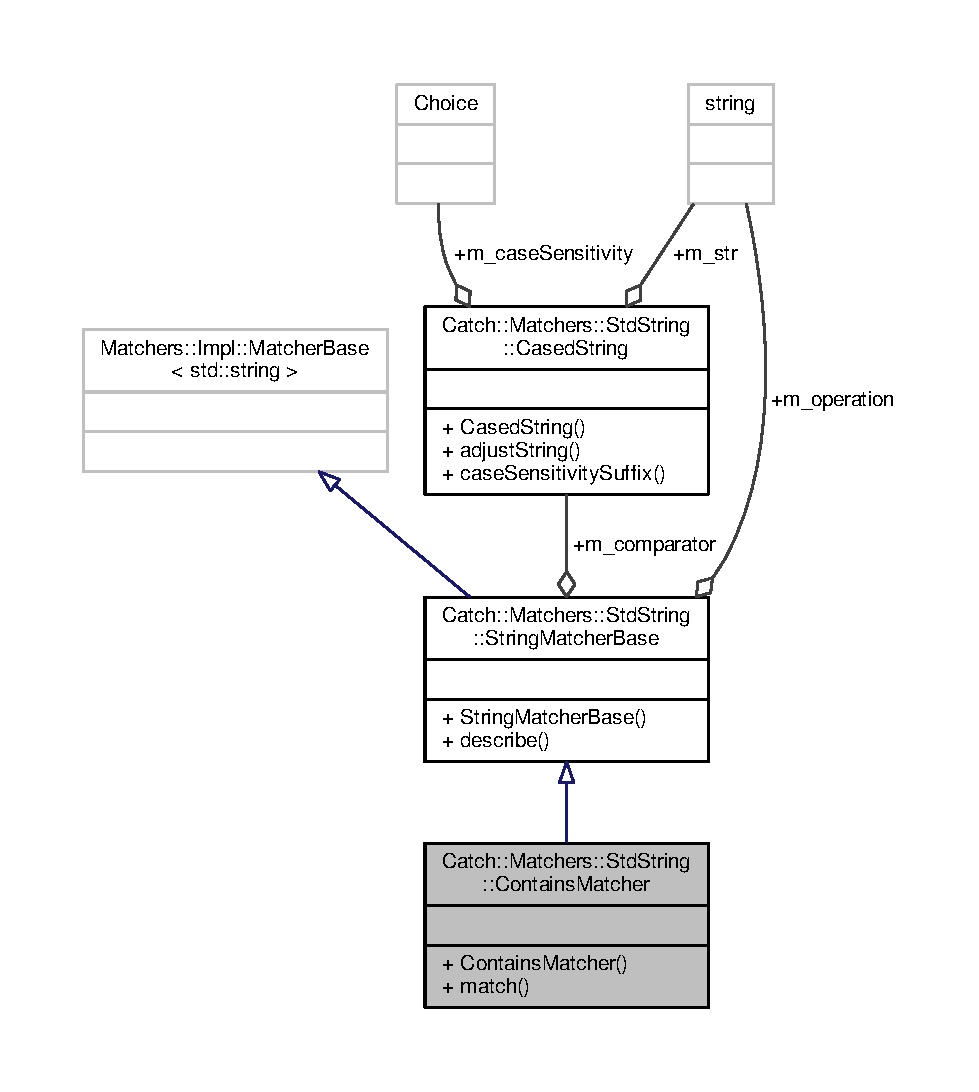
\includegraphics[width=350pt]{struct_catch_1_1_matchers_1_1_std_string_1_1_contains_matcher__coll__graph}
\end{center}
\end{figure}
\subsection*{Public Member Functions}
\begin{DoxyCompactItemize}
\item 
\hyperlink{struct_catch_1_1_matchers_1_1_std_string_1_1_contains_matcher_acc892883c8409e34b28c9b39d4ef1fe3}{Contains\-Matcher} (\hyperlink{struct_catch_1_1_matchers_1_1_std_string_1_1_cased_string}{Cased\-String} const \&comparator)
\item 
bool \hyperlink{struct_catch_1_1_matchers_1_1_std_string_1_1_contains_matcher_a630628b234b037be83fe587081a80b53}{match} (std\-::string const \&source) const override
\end{DoxyCompactItemize}
\subsection*{Additional Inherited Members}


\subsection{Constructor \& Destructor Documentation}
\hypertarget{struct_catch_1_1_matchers_1_1_std_string_1_1_contains_matcher_acc892883c8409e34b28c9b39d4ef1fe3}{\index{Catch\-::\-Matchers\-::\-Std\-String\-::\-Contains\-Matcher@{Catch\-::\-Matchers\-::\-Std\-String\-::\-Contains\-Matcher}!Contains\-Matcher@{Contains\-Matcher}}
\index{Contains\-Matcher@{Contains\-Matcher}!Catch::Matchers::StdString::ContainsMatcher@{Catch\-::\-Matchers\-::\-Std\-String\-::\-Contains\-Matcher}}
\subsubsection[{Contains\-Matcher}]{\setlength{\rightskip}{0pt plus 5cm}Catch\-::\-Matchers\-::\-Std\-String\-::\-Contains\-Matcher\-::\-Contains\-Matcher (
\begin{DoxyParamCaption}
\item[{{\bf Cased\-String} const \&}]{comparator}
\end{DoxyParamCaption}
)}}\label{struct_catch_1_1_matchers_1_1_std_string_1_1_contains_matcher_acc892883c8409e34b28c9b39d4ef1fe3}


\subsection{Member Function Documentation}
\hypertarget{struct_catch_1_1_matchers_1_1_std_string_1_1_contains_matcher_a630628b234b037be83fe587081a80b53}{\index{Catch\-::\-Matchers\-::\-Std\-String\-::\-Contains\-Matcher@{Catch\-::\-Matchers\-::\-Std\-String\-::\-Contains\-Matcher}!match@{match}}
\index{match@{match}!Catch::Matchers::StdString::ContainsMatcher@{Catch\-::\-Matchers\-::\-Std\-String\-::\-Contains\-Matcher}}
\subsubsection[{match}]{\setlength{\rightskip}{0pt plus 5cm}bool Catch\-::\-Matchers\-::\-Std\-String\-::\-Contains\-Matcher\-::match (
\begin{DoxyParamCaption}
\item[{std\-::string const \&}]{source}
\end{DoxyParamCaption}
) const\hspace{0.3cm}{\ttfamily [override]}}}\label{struct_catch_1_1_matchers_1_1_std_string_1_1_contains_matcher_a630628b234b037be83fe587081a80b53}


The documentation for this struct was generated from the following file\-:\begin{DoxyCompactItemize}
\item 
\hyperlink{catch_8hpp}{catch.\-hpp}\end{DoxyCompactItemize}

\hypertarget{struct_catch_1_1_matchers_1_1_vector_1_1_contains_matcher}{\section{Catch\-:\-:Matchers\-:\-:Vector\-:\-:Contains\-Matcher$<$ T $>$ Struct Template Reference}
\label{struct_catch_1_1_matchers_1_1_vector_1_1_contains_matcher}\index{Catch\-::\-Matchers\-::\-Vector\-::\-Contains\-Matcher$<$ T $>$@{Catch\-::\-Matchers\-::\-Vector\-::\-Contains\-Matcher$<$ T $>$}}
}


{\ttfamily \#include $<$catch.\-hpp$>$}



Inheritance diagram for Catch\-:\-:Matchers\-:\-:Vector\-:\-:Contains\-Matcher$<$ T $>$\-:
\nopagebreak
\begin{figure}[H]
\begin{center}
\leavevmode
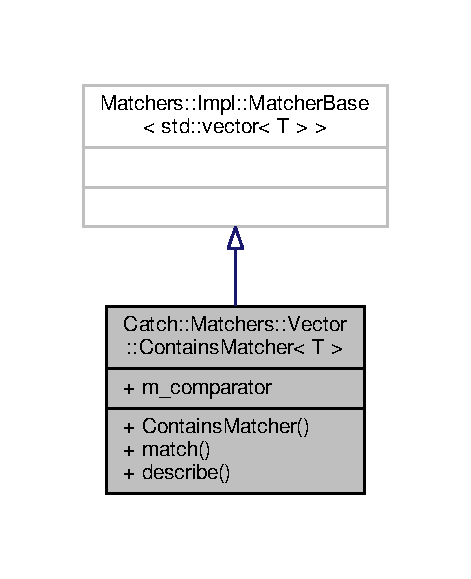
\includegraphics[width=226pt]{struct_catch_1_1_matchers_1_1_vector_1_1_contains_matcher__inherit__graph}
\end{center}
\end{figure}


Collaboration diagram for Catch\-:\-:Matchers\-:\-:Vector\-:\-:Contains\-Matcher$<$ T $>$\-:
\nopagebreak
\begin{figure}[H]
\begin{center}
\leavevmode
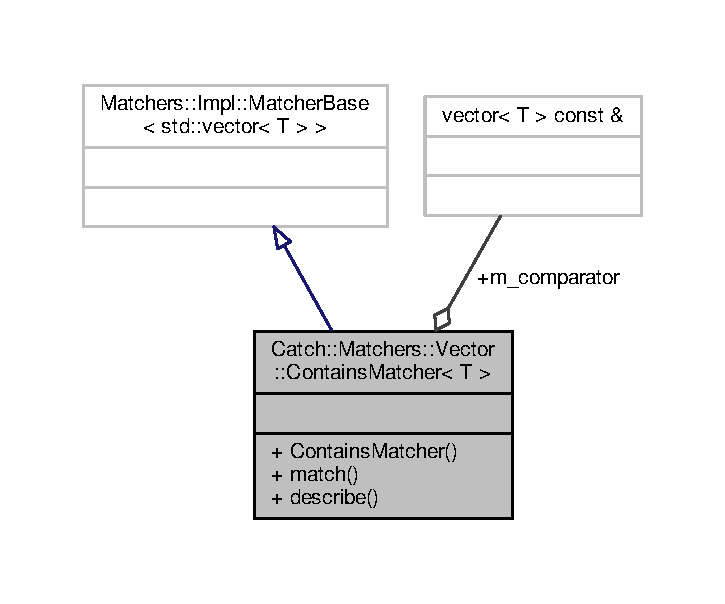
\includegraphics[width=348pt]{struct_catch_1_1_matchers_1_1_vector_1_1_contains_matcher__coll__graph}
\end{center}
\end{figure}
\subsection*{Public Member Functions}
\begin{DoxyCompactItemize}
\item 
\hyperlink{struct_catch_1_1_matchers_1_1_vector_1_1_contains_matcher_ad8e92c8399be6dce75bb5702cdfab700}{Contains\-Matcher} (std\-::vector$<$ T $>$ const \&comparator)
\item 
bool \hyperlink{struct_catch_1_1_matchers_1_1_vector_1_1_contains_matcher_afd33467ae48a41a634572b41b053f67f}{match} (std\-::vector$<$ T $>$ const \&v) const override
\item 
std\-::string \hyperlink{struct_catch_1_1_matchers_1_1_vector_1_1_contains_matcher_abe6a9ea3d6506c9a1f75ff524f35832e}{describe} () const override
\end{DoxyCompactItemize}
\subsection*{Public Attributes}
\begin{DoxyCompactItemize}
\item 
std\-::vector$<$ T $>$ const \& \hyperlink{struct_catch_1_1_matchers_1_1_vector_1_1_contains_matcher_a83d051166e4ed0d535219ad6ee99abb2}{m\-\_\-comparator}
\end{DoxyCompactItemize}


\subsection{Constructor \& Destructor Documentation}
\hypertarget{struct_catch_1_1_matchers_1_1_vector_1_1_contains_matcher_ad8e92c8399be6dce75bb5702cdfab700}{\index{Catch\-::\-Matchers\-::\-Vector\-::\-Contains\-Matcher@{Catch\-::\-Matchers\-::\-Vector\-::\-Contains\-Matcher}!Contains\-Matcher@{Contains\-Matcher}}
\index{Contains\-Matcher@{Contains\-Matcher}!Catch::Matchers::Vector::ContainsMatcher@{Catch\-::\-Matchers\-::\-Vector\-::\-Contains\-Matcher}}
\subsubsection[{Contains\-Matcher}]{\setlength{\rightskip}{0pt plus 5cm}template$<$typename T $>$ {\bf Catch\-::\-Matchers\-::\-Vector\-::\-Contains\-Matcher}$<$ T $>$\-::{\bf Contains\-Matcher} (
\begin{DoxyParamCaption}
\item[{std\-::vector$<$ T $>$ const \&}]{comparator}
\end{DoxyParamCaption}
)\hspace{0.3cm}{\ttfamily [inline]}}}\label{struct_catch_1_1_matchers_1_1_vector_1_1_contains_matcher_ad8e92c8399be6dce75bb5702cdfab700}

\begin{DoxyCode}
2577 : \hyperlink{struct_catch_1_1_matchers_1_1_vector_1_1_contains_matcher_a83d051166e4ed0d535219ad6ee99abb2}{m\_comparator}(comparator) \{\}
\end{DoxyCode}


\subsection{Member Function Documentation}
\hypertarget{struct_catch_1_1_matchers_1_1_vector_1_1_contains_matcher_abe6a9ea3d6506c9a1f75ff524f35832e}{\index{Catch\-::\-Matchers\-::\-Vector\-::\-Contains\-Matcher@{Catch\-::\-Matchers\-::\-Vector\-::\-Contains\-Matcher}!describe@{describe}}
\index{describe@{describe}!Catch::Matchers::Vector::ContainsMatcher@{Catch\-::\-Matchers\-::\-Vector\-::\-Contains\-Matcher}}
\subsubsection[{describe}]{\setlength{\rightskip}{0pt plus 5cm}template$<$typename T $>$ std\-::string {\bf Catch\-::\-Matchers\-::\-Vector\-::\-Contains\-Matcher}$<$ T $>$\-::describe (
\begin{DoxyParamCaption}
{}
\end{DoxyParamCaption}
) const\hspace{0.3cm}{\ttfamily [inline]}, {\ttfamily [override]}}}\label{struct_catch_1_1_matchers_1_1_vector_1_1_contains_matcher_abe6a9ea3d6506c9a1f75ff524f35832e}


References Catch\-::\-Detail\-::stringify().


\begin{DoxyCode}
2597                                                     \{
2598                     \textcolor{keywordflow}{return} \textcolor{stringliteral}{"Contains: "} + \hyperlink{namespace_catch_1_1_detail_af0ad48344ffd3f92f3568465248a9880}{::Catch::Detail::stringify}(
      \hyperlink{struct_catch_1_1_matchers_1_1_vector_1_1_contains_matcher_a83d051166e4ed0d535219ad6ee99abb2}{m\_comparator});
2599                 \}
\end{DoxyCode}
\hypertarget{struct_catch_1_1_matchers_1_1_vector_1_1_contains_matcher_afd33467ae48a41a634572b41b053f67f}{\index{Catch\-::\-Matchers\-::\-Vector\-::\-Contains\-Matcher@{Catch\-::\-Matchers\-::\-Vector\-::\-Contains\-Matcher}!match@{match}}
\index{match@{match}!Catch::Matchers::Vector::ContainsMatcher@{Catch\-::\-Matchers\-::\-Vector\-::\-Contains\-Matcher}}
\subsubsection[{match}]{\setlength{\rightskip}{0pt plus 5cm}template$<$typename T $>$ bool {\bf Catch\-::\-Matchers\-::\-Vector\-::\-Contains\-Matcher}$<$ T $>$\-::match (
\begin{DoxyParamCaption}
\item[{std\-::vector$<$ T $>$ const \&}]{v}
\end{DoxyParamCaption}
) const\hspace{0.3cm}{\ttfamily [inline]}, {\ttfamily [override]}}}\label{struct_catch_1_1_matchers_1_1_vector_1_1_contains_matcher_afd33467ae48a41a634572b41b053f67f}

\begin{DoxyCode}
2579                                                                  \{
2580                     \textcolor{comment}{// !TBD: see note in EqualsMatcher}
2581                     \textcolor{keywordflow}{if} (\hyperlink{struct_catch_1_1_matchers_1_1_vector_1_1_contains_matcher_a83d051166e4ed0d535219ad6ee99abb2}{m\_comparator}.size() > v.size())
2582                         \textcolor{keywordflow}{return} \textcolor{keyword}{false};
2583                     \textcolor{keywordflow}{for} (\textcolor{keyword}{auto} \textcolor{keyword}{const}& comparator : \hyperlink{struct_catch_1_1_matchers_1_1_vector_1_1_contains_matcher_a83d051166e4ed0d535219ad6ee99abb2}{m\_comparator}) \{
2584                         \textcolor{keyword}{auto} present = \textcolor{keyword}{false};
2585                         \textcolor{keywordflow}{for} (\textcolor{keyword}{const} \textcolor{keyword}{auto}& el : v) \{
2586                             \textcolor{keywordflow}{if} (el == comparator) \{
2587                                 present = \textcolor{keyword}{true};
2588                                 \textcolor{keywordflow}{break};
2589                             \}
2590                         \}
2591                         \textcolor{keywordflow}{if} (!present) \{
2592                             \textcolor{keywordflow}{return} \textcolor{keyword}{false};
2593                         \}
2594                     \}
2595                     \textcolor{keywordflow}{return} \textcolor{keyword}{true};
2596                 \}
\end{DoxyCode}


\subsection{Member Data Documentation}
\hypertarget{struct_catch_1_1_matchers_1_1_vector_1_1_contains_matcher_a83d051166e4ed0d535219ad6ee99abb2}{\index{Catch\-::\-Matchers\-::\-Vector\-::\-Contains\-Matcher@{Catch\-::\-Matchers\-::\-Vector\-::\-Contains\-Matcher}!m\-\_\-comparator@{m\-\_\-comparator}}
\index{m\-\_\-comparator@{m\-\_\-comparator}!Catch::Matchers::Vector::ContainsMatcher@{Catch\-::\-Matchers\-::\-Vector\-::\-Contains\-Matcher}}
\subsubsection[{m\-\_\-comparator}]{\setlength{\rightskip}{0pt plus 5cm}template$<$typename T $>$ std\-::vector$<$T$>$ const\& {\bf Catch\-::\-Matchers\-::\-Vector\-::\-Contains\-Matcher}$<$ T $>$\-::m\-\_\-comparator}}\label{struct_catch_1_1_matchers_1_1_vector_1_1_contains_matcher_a83d051166e4ed0d535219ad6ee99abb2}


The documentation for this struct was generated from the following file\-:\begin{DoxyCompactItemize}
\item 
\hyperlink{catch_8hpp}{catch.\-hpp}\end{DoxyCompactItemize}

\hypertarget{struct_catch_1_1_counts}{\section{Catch\-:\-:Counts Struct Reference}
\label{struct_catch_1_1_counts}\index{Catch\-::\-Counts@{Catch\-::\-Counts}}
}


{\ttfamily \#include $<$catch.\-hpp$>$}



Collaboration diagram for Catch\-:\-:Counts\-:
\nopagebreak
\begin{figure}[H]
\begin{center}
\leavevmode
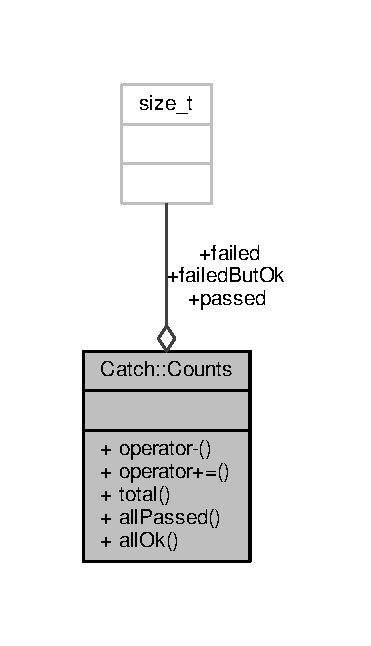
\includegraphics[width=178pt]{struct_catch_1_1_counts__coll__graph}
\end{center}
\end{figure}
\subsection*{Public Member Functions}
\begin{DoxyCompactItemize}
\item 
\hyperlink{struct_catch_1_1_counts}{Counts} \hyperlink{struct_catch_1_1_counts_aedf86fefe33938d132a6981171cd83e6}{operator-\/} (\hyperlink{struct_catch_1_1_counts}{Counts} const \&other) const 
\item 
\hyperlink{struct_catch_1_1_counts}{Counts} \& \hyperlink{struct_catch_1_1_counts_a322a89475cd2cc039140ef371e973677}{operator+=} (\hyperlink{struct_catch_1_1_counts}{Counts} const \&other)
\item 
std\-::size\-\_\-t \hyperlink{struct_catch_1_1_counts_a9125c662e30114e5c5cc94729b1e9e84}{total} () const 
\item 
bool \hyperlink{struct_catch_1_1_counts_adbbaca552f6017ce69e0d5dc5500bea4}{all\-Passed} () const 
\item 
bool \hyperlink{struct_catch_1_1_counts_ab2497c9dfc77be757a90225ea69595f5}{all\-Ok} () const 
\end{DoxyCompactItemize}
\subsection*{Public Attributes}
\begin{DoxyCompactItemize}
\item 
std\-::size\-\_\-t \hyperlink{struct_catch_1_1_counts_ad28daaf3de28006400208b6dd0c631e6}{passed} = 0
\item 
std\-::size\-\_\-t \hyperlink{struct_catch_1_1_counts_a19982a3817a3bc2c07f0290e71f497a3}{failed} = 0
\item 
std\-::size\-\_\-t \hyperlink{struct_catch_1_1_counts_ac090973a2ff51394cd452718e75c073e}{failed\-But\-Ok} = 0
\end{DoxyCompactItemize}


\subsection{Member Function Documentation}
\hypertarget{struct_catch_1_1_counts_ab2497c9dfc77be757a90225ea69595f5}{\index{Catch\-::\-Counts@{Catch\-::\-Counts}!all\-Ok@{all\-Ok}}
\index{all\-Ok@{all\-Ok}!Catch::Counts@{Catch\-::\-Counts}}
\subsubsection[{all\-Ok}]{\setlength{\rightskip}{0pt plus 5cm}bool Catch\-::\-Counts\-::all\-Ok (
\begin{DoxyParamCaption}
{}
\end{DoxyParamCaption}
) const}}\label{struct_catch_1_1_counts_ab2497c9dfc77be757a90225ea69595f5}
\hypertarget{struct_catch_1_1_counts_adbbaca552f6017ce69e0d5dc5500bea4}{\index{Catch\-::\-Counts@{Catch\-::\-Counts}!all\-Passed@{all\-Passed}}
\index{all\-Passed@{all\-Passed}!Catch::Counts@{Catch\-::\-Counts}}
\subsubsection[{all\-Passed}]{\setlength{\rightskip}{0pt plus 5cm}bool Catch\-::\-Counts\-::all\-Passed (
\begin{DoxyParamCaption}
{}
\end{DoxyParamCaption}
) const}}\label{struct_catch_1_1_counts_adbbaca552f6017ce69e0d5dc5500bea4}
\hypertarget{struct_catch_1_1_counts_a322a89475cd2cc039140ef371e973677}{\index{Catch\-::\-Counts@{Catch\-::\-Counts}!operator+=@{operator+=}}
\index{operator+=@{operator+=}!Catch::Counts@{Catch\-::\-Counts}}
\subsubsection[{operator+=}]{\setlength{\rightskip}{0pt plus 5cm}{\bf Counts}\& Catch\-::\-Counts\-::operator+= (
\begin{DoxyParamCaption}
\item[{{\bf Counts} const \&}]{other}
\end{DoxyParamCaption}
)}}\label{struct_catch_1_1_counts_a322a89475cd2cc039140ef371e973677}
\hypertarget{struct_catch_1_1_counts_aedf86fefe33938d132a6981171cd83e6}{\index{Catch\-::\-Counts@{Catch\-::\-Counts}!operator-\/@{operator-\/}}
\index{operator-\/@{operator-\/}!Catch::Counts@{Catch\-::\-Counts}}
\subsubsection[{operator-\/}]{\setlength{\rightskip}{0pt plus 5cm}{\bf Counts} Catch\-::\-Counts\-::operator-\/ (
\begin{DoxyParamCaption}
\item[{{\bf Counts} const \&}]{other}
\end{DoxyParamCaption}
) const}}\label{struct_catch_1_1_counts_aedf86fefe33938d132a6981171cd83e6}
\hypertarget{struct_catch_1_1_counts_a9125c662e30114e5c5cc94729b1e9e84}{\index{Catch\-::\-Counts@{Catch\-::\-Counts}!total@{total}}
\index{total@{total}!Catch::Counts@{Catch\-::\-Counts}}
\subsubsection[{total}]{\setlength{\rightskip}{0pt plus 5cm}std\-::size\-\_\-t Catch\-::\-Counts\-::total (
\begin{DoxyParamCaption}
{}
\end{DoxyParamCaption}
) const}}\label{struct_catch_1_1_counts_a9125c662e30114e5c5cc94729b1e9e84}


\subsection{Member Data Documentation}
\hypertarget{struct_catch_1_1_counts_a19982a3817a3bc2c07f0290e71f497a3}{\index{Catch\-::\-Counts@{Catch\-::\-Counts}!failed@{failed}}
\index{failed@{failed}!Catch::Counts@{Catch\-::\-Counts}}
\subsubsection[{failed}]{\setlength{\rightskip}{0pt plus 5cm}std\-::size\-\_\-t Catch\-::\-Counts\-::failed = 0}}\label{struct_catch_1_1_counts_a19982a3817a3bc2c07f0290e71f497a3}
\hypertarget{struct_catch_1_1_counts_ac090973a2ff51394cd452718e75c073e}{\index{Catch\-::\-Counts@{Catch\-::\-Counts}!failed\-But\-Ok@{failed\-But\-Ok}}
\index{failed\-But\-Ok@{failed\-But\-Ok}!Catch::Counts@{Catch\-::\-Counts}}
\subsubsection[{failed\-But\-Ok}]{\setlength{\rightskip}{0pt plus 5cm}std\-::size\-\_\-t Catch\-::\-Counts\-::failed\-But\-Ok = 0}}\label{struct_catch_1_1_counts_ac090973a2ff51394cd452718e75c073e}
\hypertarget{struct_catch_1_1_counts_ad28daaf3de28006400208b6dd0c631e6}{\index{Catch\-::\-Counts@{Catch\-::\-Counts}!passed@{passed}}
\index{passed@{passed}!Catch::Counts@{Catch\-::\-Counts}}
\subsubsection[{passed}]{\setlength{\rightskip}{0pt plus 5cm}std\-::size\-\_\-t Catch\-::\-Counts\-::passed = 0}}\label{struct_catch_1_1_counts_ad28daaf3de28006400208b6dd0c631e6}


The documentation for this struct was generated from the following file\-:\begin{DoxyCompactItemize}
\item 
\hyperlink{catch_8hpp}{catch.\-hpp}\end{DoxyCompactItemize}

\hypertarget{struct_catch_1_1_decomposer}{\section{Catch\-:\-:Decomposer Struct Reference}
\label{struct_catch_1_1_decomposer}\index{Catch\-::\-Decomposer@{Catch\-::\-Decomposer}}
}


{\ttfamily \#include $<$catch.\-hpp$>$}



Collaboration diagram for Catch\-:\-:Decomposer\-:
\nopagebreak
\begin{figure}[H]
\begin{center}
\leavevmode
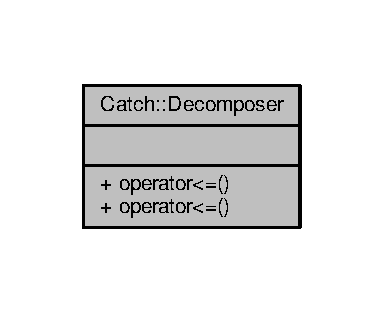
\includegraphics[width=184pt]{struct_catch_1_1_decomposer__coll__graph}
\end{center}
\end{figure}
\subsection*{Public Member Functions}
\begin{DoxyCompactItemize}
\item 
{\footnotesize template$<$typename T $>$ }\\auto \hyperlink{struct_catch_1_1_decomposer_a4b1e5e844c20e5a90e3d759d216674cd}{operator$<$=} (T const \&lhs) -\/$>$ \hyperlink{class_catch_1_1_expr_lhs}{Expr\-Lhs}$<$ T const \& $>$
\item 
auto \hyperlink{struct_catch_1_1_decomposer_aac129b94903ae1339d5709049d83613b}{operator$<$=} (bool value) -\/$>$ \hyperlink{class_catch_1_1_expr_lhs}{Expr\-Lhs}$<$ bool $>$
\end{DoxyCompactItemize}


\subsection{Member Function Documentation}
\hypertarget{struct_catch_1_1_decomposer_a4b1e5e844c20e5a90e3d759d216674cd}{\index{Catch\-::\-Decomposer@{Catch\-::\-Decomposer}!operator$<$=@{operator$<$=}}
\index{operator$<$=@{operator$<$=}!Catch::Decomposer@{Catch\-::\-Decomposer}}
\subsubsection[{operator$<$=}]{\setlength{\rightskip}{0pt plus 5cm}template$<$typename T $>$ auto Catch\-::\-Decomposer\-::operator$<$= (
\begin{DoxyParamCaption}
\item[{T const \&}]{lhs}
\end{DoxyParamCaption}
) -\/$>$ {\bf Expr\-Lhs}$<$T const\&$>$ \hspace{0.3cm}{\ttfamily [inline]}}}\label{struct_catch_1_1_decomposer_a4b1e5e844c20e5a90e3d759d216674cd}

\begin{DoxyCode}
1433                                                              \{
1434             \textcolor{keywordflow}{return} ExprLhs<T const&>\{ lhs \};
1435         \}
\end{DoxyCode}
\hypertarget{struct_catch_1_1_decomposer_aac129b94903ae1339d5709049d83613b}{\index{Catch\-::\-Decomposer@{Catch\-::\-Decomposer}!operator$<$=@{operator$<$=}}
\index{operator$<$=@{operator$<$=}!Catch::Decomposer@{Catch\-::\-Decomposer}}
\subsubsection[{operator$<$=}]{\setlength{\rightskip}{0pt plus 5cm}auto Catch\-::\-Decomposer\-::operator$<$= (
\begin{DoxyParamCaption}
\item[{bool}]{value}
\end{DoxyParamCaption}
) -\/$>$ {\bf Expr\-Lhs}$<$bool$>$ \hspace{0.3cm}{\ttfamily [inline]}}}\label{struct_catch_1_1_decomposer_aac129b94903ae1339d5709049d83613b}

\begin{DoxyCode}
1437                                                       \{
1438             \textcolor{keywordflow}{return} ExprLhs<bool>\{ value \};
1439         \}
\end{DoxyCode}


The documentation for this struct was generated from the following file\-:\begin{DoxyCompactItemize}
\item 
\hyperlink{catch_8hpp}{catch.\-hpp}\end{DoxyCompactItemize}

\hypertarget{struct_catch_1_1_matchers_1_1_std_string_1_1_ends_with_matcher}{\section{Catch\-:\-:Matchers\-:\-:Std\-String\-:\-:Ends\-With\-Matcher Struct Reference}
\label{struct_catch_1_1_matchers_1_1_std_string_1_1_ends_with_matcher}\index{Catch\-::\-Matchers\-::\-Std\-String\-::\-Ends\-With\-Matcher@{Catch\-::\-Matchers\-::\-Std\-String\-::\-Ends\-With\-Matcher}}
}


{\ttfamily \#include $<$catch.\-hpp$>$}



Inheritance diagram for Catch\-:\-:Matchers\-:\-:Std\-String\-:\-:Ends\-With\-Matcher\-:
\nopagebreak
\begin{figure}[H]
\begin{center}
\leavevmode
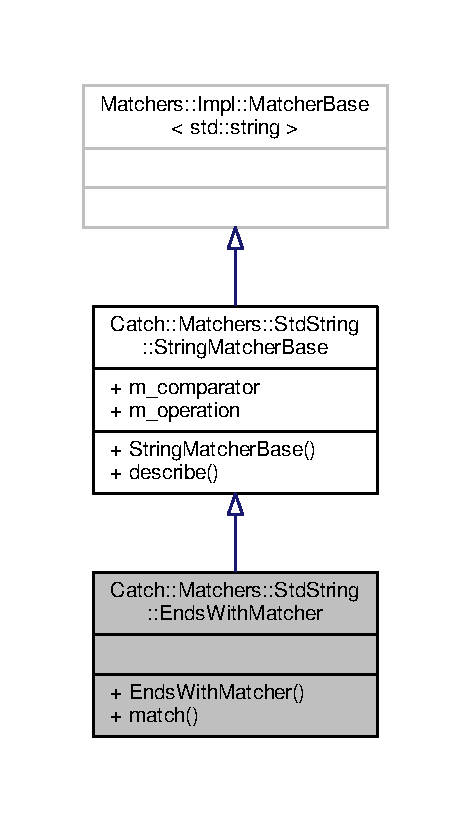
\includegraphics[width=226pt]{struct_catch_1_1_matchers_1_1_std_string_1_1_ends_with_matcher__inherit__graph}
\end{center}
\end{figure}


Collaboration diagram for Catch\-:\-:Matchers\-:\-:Std\-String\-:\-:Ends\-With\-Matcher\-:
\nopagebreak
\begin{figure}[H]
\begin{center}
\leavevmode
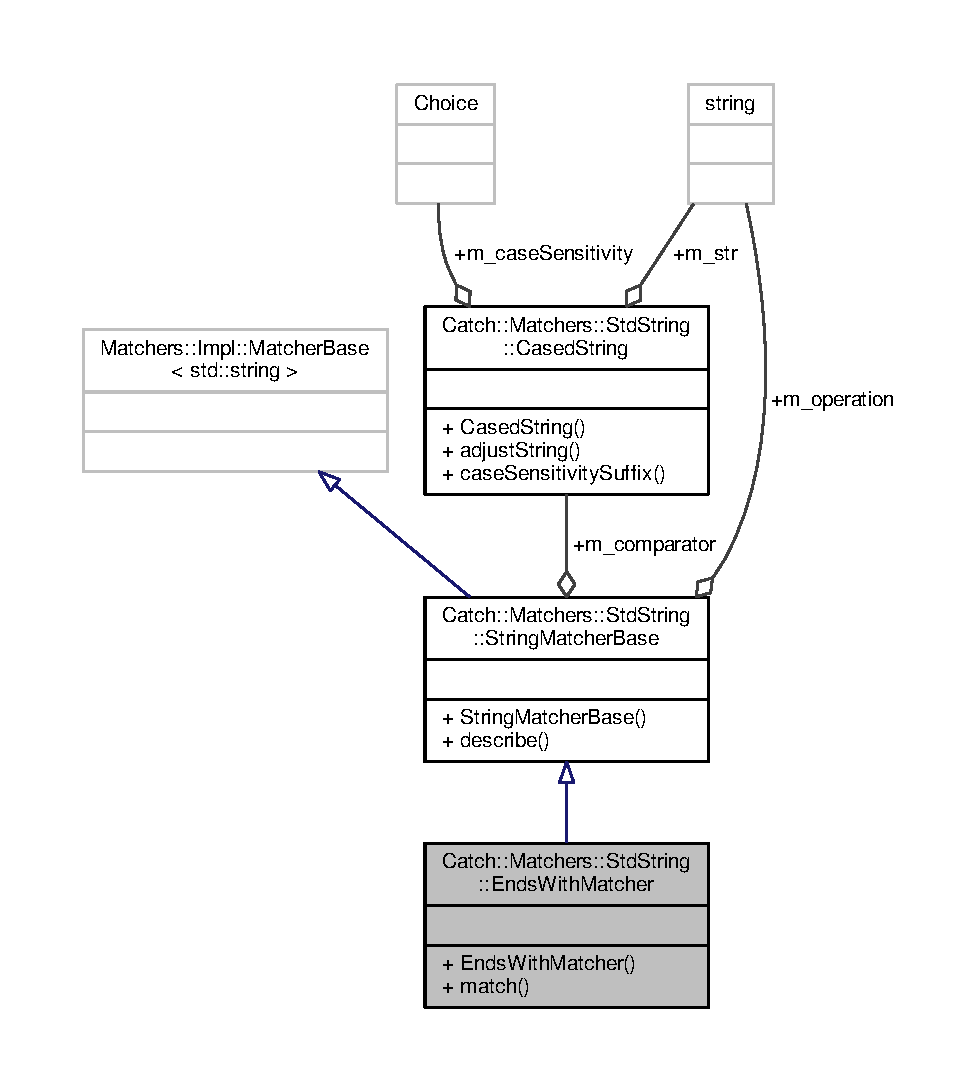
\includegraphics[width=350pt]{struct_catch_1_1_matchers_1_1_std_string_1_1_ends_with_matcher__coll__graph}
\end{center}
\end{figure}
\subsection*{Public Member Functions}
\begin{DoxyCompactItemize}
\item 
\hyperlink{struct_catch_1_1_matchers_1_1_std_string_1_1_ends_with_matcher_aa5ec700b4629562f74f362080accfd7b}{Ends\-With\-Matcher} (\hyperlink{struct_catch_1_1_matchers_1_1_std_string_1_1_cased_string}{Cased\-String} const \&comparator)
\item 
bool \hyperlink{struct_catch_1_1_matchers_1_1_std_string_1_1_ends_with_matcher_aca2741fa57374a2a98d2a84ac3e13a6d}{match} (std\-::string const \&source) const override
\end{DoxyCompactItemize}
\subsection*{Additional Inherited Members}


\subsection{Constructor \& Destructor Documentation}
\hypertarget{struct_catch_1_1_matchers_1_1_std_string_1_1_ends_with_matcher_aa5ec700b4629562f74f362080accfd7b}{\index{Catch\-::\-Matchers\-::\-Std\-String\-::\-Ends\-With\-Matcher@{Catch\-::\-Matchers\-::\-Std\-String\-::\-Ends\-With\-Matcher}!Ends\-With\-Matcher@{Ends\-With\-Matcher}}
\index{Ends\-With\-Matcher@{Ends\-With\-Matcher}!Catch::Matchers::StdString::EndsWithMatcher@{Catch\-::\-Matchers\-::\-Std\-String\-::\-Ends\-With\-Matcher}}
\subsubsection[{Ends\-With\-Matcher}]{\setlength{\rightskip}{0pt plus 5cm}Catch\-::\-Matchers\-::\-Std\-String\-::\-Ends\-With\-Matcher\-::\-Ends\-With\-Matcher (
\begin{DoxyParamCaption}
\item[{{\bf Cased\-String} const \&}]{comparator}
\end{DoxyParamCaption}
)}}\label{struct_catch_1_1_matchers_1_1_std_string_1_1_ends_with_matcher_aa5ec700b4629562f74f362080accfd7b}


\subsection{Member Function Documentation}
\hypertarget{struct_catch_1_1_matchers_1_1_std_string_1_1_ends_with_matcher_aca2741fa57374a2a98d2a84ac3e13a6d}{\index{Catch\-::\-Matchers\-::\-Std\-String\-::\-Ends\-With\-Matcher@{Catch\-::\-Matchers\-::\-Std\-String\-::\-Ends\-With\-Matcher}!match@{match}}
\index{match@{match}!Catch::Matchers::StdString::EndsWithMatcher@{Catch\-::\-Matchers\-::\-Std\-String\-::\-Ends\-With\-Matcher}}
\subsubsection[{match}]{\setlength{\rightskip}{0pt plus 5cm}bool Catch\-::\-Matchers\-::\-Std\-String\-::\-Ends\-With\-Matcher\-::match (
\begin{DoxyParamCaption}
\item[{std\-::string const \&}]{source}
\end{DoxyParamCaption}
) const\hspace{0.3cm}{\ttfamily [override]}}}\label{struct_catch_1_1_matchers_1_1_std_string_1_1_ends_with_matcher_aca2741fa57374a2a98d2a84ac3e13a6d}


The documentation for this struct was generated from the following file\-:\begin{DoxyCompactItemize}
\item 
\hyperlink{catch_8hpp}{catch.\-hpp}\end{DoxyCompactItemize}

\hypertarget{class_enemy}{\section{Enemy Class Reference}
\label{class_enemy}\index{Enemy@{Enemy}}
}


{\ttfamily \#include $<$Enemy.\-h$>$}



Collaboration diagram for Enemy\-:
\nopagebreak
\begin{figure}[H]
\begin{center}
\leavevmode
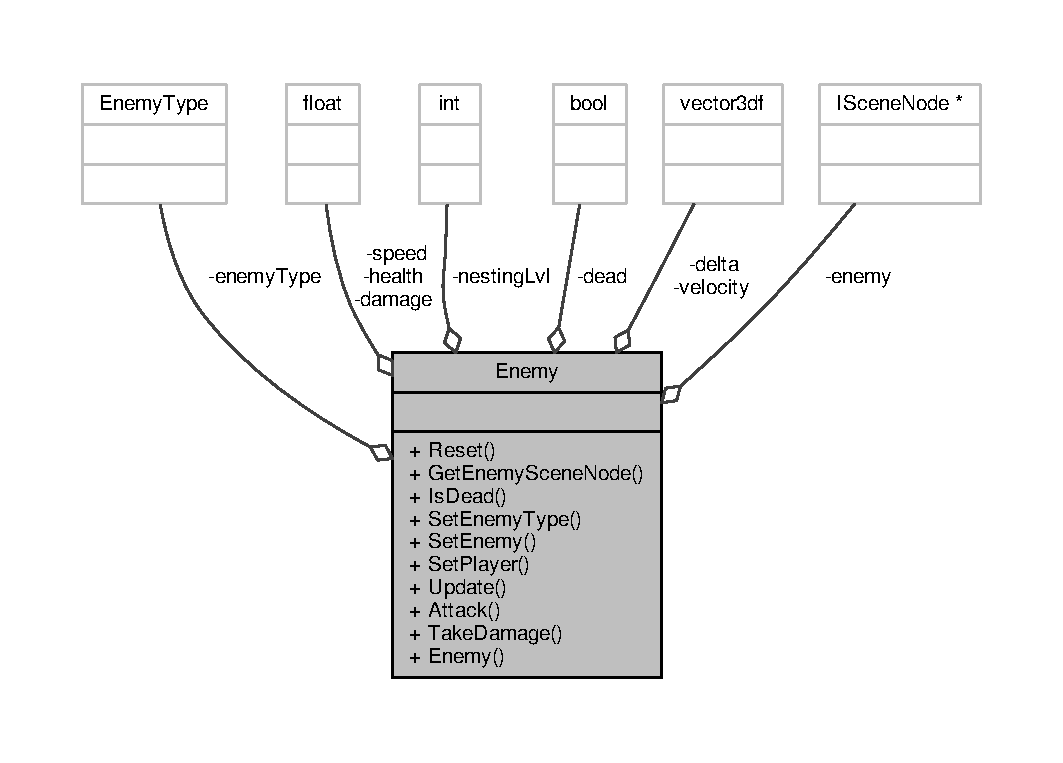
\includegraphics[width=350pt]{class_enemy__coll__graph}
\end{center}
\end{figure}
\subsection*{Public Types}
\begin{DoxyCompactItemize}
\item 
enum \hyperlink{class_enemy_a98c2ee2c2081001de17a4bc9fa8da94f}{Enemy\-Type} \{ \hyperlink{class_enemy_a98c2ee2c2081001de17a4bc9fa8da94fae39ca3e105330b4913cf2d7496d2e49f}{basic}, 
\hyperlink{class_enemy_a98c2ee2c2081001de17a4bc9fa8da94fa227c1851ffd53fcbc3b04e09be3426f7}{fast}, 
\hyperlink{class_enemy_a98c2ee2c2081001de17a4bc9fa8da94fa46f876a597075a60b04ee647a34dfad9}{tanky}, 
\hyperlink{class_enemy_a98c2ee2c2081001de17a4bc9fa8da94fabed20a625942a91cdb7b85a000d8bde8}{matroshka}
 \}
\end{DoxyCompactItemize}
\subsection*{Public Member Functions}
\begin{DoxyCompactItemize}
\item 
void \hyperlink{class_enemy_af6c878494349e5158e9e2f5ccbebe22d}{Reset} ()
\item 
irr\-::scene\-::\-I\-Scene\-Node $\ast$ \hyperlink{class_enemy_a85b8d7d8c6a61f8824a3b7b3fea795f4}{Get\-Enemy\-Scene\-Node} ()
\item 
bool \hyperlink{class_enemy_a019dd82194ff8415b0439cc375a88545}{Is\-Dead} ()
\item 
void \hyperlink{class_enemy_a567a82f1d7cb9034509459850f7784fc}{Set\-Enemy\-Type} (\hyperlink{class_enemy_a98c2ee2c2081001de17a4bc9fa8da94f}{Enemy\-Type} type, int nest\-Amount=0)
\item 
void \hyperlink{class_enemy_a927846998a0a936374a5734fb832b151}{Set\-Enemy} (irr\-::scene\-::\-I\-Scene\-Node $\ast$new\-Enemy)
\item 
void \hyperlink{class_enemy_a421d67f70801a3399ca22067fcde6dff}{Set\-Player} (\hyperlink{class_player}{Player} $\ast$\hyperlink{_enemy_spawner_8cpp_a9cd078164ceb4e9bfed2981b94610dc9}{\-\_\-player})
\item 
void \hyperlink{class_enemy_a2429c6f39d0b763f899bef2c035fa9c8}{Update} (float \hyperlink{_player_8cpp_adc988571147642cda93afbf89783f9c9}{frame\-Delta\-Time})
\item 
void \hyperlink{class_enemy_a9d077112e9af9e0bf92aa73ec20ea6ae}{Attack} ()
\item 
void \hyperlink{class_enemy_ab3567fe4213734615d7f3fed6c48a9c8}{Take\-Damage} (irr\-::f32 \hyperlink{class_enemy_a5d5917c222119c1d8eb3183c27c7adb7}{damage})
\item 
\hyperlink{class_enemy_a549b49efc0292397f778ddab5af279de}{Enemy} (irr\-::\-Irrlicht\-Device $\ast$device)
\end{DoxyCompactItemize}
\subsection*{Private Attributes}
\begin{DoxyCompactItemize}
\item 
irr\-::scene\-::\-I\-Scene\-Node $\ast$ \hyperlink{class_enemy_a4befe0ced393215de590152256bf1ee4}{enemy}
\item 
irr\-::core\-::vector3df \hyperlink{class_enemy_a01b8136e0754f278e48b63f25e2361bc}{velocity}
\item 
irr\-::core\-::vector3df \hyperlink{class_enemy_a2aeaae8acd857242e40db8b034566351}{delta}
\item 
\hyperlink{class_enemy_a98c2ee2c2081001de17a4bc9fa8da94f}{Enemy\-Type} \hyperlink{class_enemy_a36bcaf317708c0ed35835bc0f79c7719}{enemy\-Type}
\item 
bool \hyperlink{class_enemy_a4b1b61e7bc79aca01f3e4b3ef19cb787}{dead}
\item 
float \hyperlink{class_enemy_a131756bf793f8d63a3b9a2b728992380}{health}
\item 
float \hyperlink{class_enemy_a98766d083fc49e746a37d0dc69be09e0}{speed}
\item 
float \hyperlink{class_enemy_a5d5917c222119c1d8eb3183c27c7adb7}{damage}
\item 
int \hyperlink{class_enemy_a28a5b00705199ef986435768edb53d48}{nesting\-Lvl}
\end{DoxyCompactItemize}


\subsection{Member Enumeration Documentation}
\hypertarget{class_enemy_a98c2ee2c2081001de17a4bc9fa8da94f}{\index{Enemy@{Enemy}!Enemy\-Type@{Enemy\-Type}}
\index{Enemy\-Type@{Enemy\-Type}!Enemy@{Enemy}}
\subsubsection[{Enemy\-Type}]{\setlength{\rightskip}{0pt plus 5cm}enum {\bf Enemy\-::\-Enemy\-Type}}}\label{class_enemy_a98c2ee2c2081001de17a4bc9fa8da94f}
\begin{Desc}
\item[Enumerator]\par
\begin{description}
\index{basic@{basic}!Enemy@{Enemy}}\index{Enemy@{Enemy}!basic@{basic}}\item[{\em 
\hypertarget{class_enemy_a98c2ee2c2081001de17a4bc9fa8da94fae39ca3e105330b4913cf2d7496d2e49f}{basic}\label{class_enemy_a98c2ee2c2081001de17a4bc9fa8da94fae39ca3e105330b4913cf2d7496d2e49f}
}]\index{fast@{fast}!Enemy@{Enemy}}\index{Enemy@{Enemy}!fast@{fast}}\item[{\em 
\hypertarget{class_enemy_a98c2ee2c2081001de17a4bc9fa8da94fa227c1851ffd53fcbc3b04e09be3426f7}{fast}\label{class_enemy_a98c2ee2c2081001de17a4bc9fa8da94fa227c1851ffd53fcbc3b04e09be3426f7}
}]\index{tanky@{tanky}!Enemy@{Enemy}}\index{Enemy@{Enemy}!tanky@{tanky}}\item[{\em 
\hypertarget{class_enemy_a98c2ee2c2081001de17a4bc9fa8da94fa46f876a597075a60b04ee647a34dfad9}{tanky}\label{class_enemy_a98c2ee2c2081001de17a4bc9fa8da94fa46f876a597075a60b04ee647a34dfad9}
}]\index{matroshka@{matroshka}!Enemy@{Enemy}}\index{Enemy@{Enemy}!matroshka@{matroshka}}\item[{\em 
\hypertarget{class_enemy_a98c2ee2c2081001de17a4bc9fa8da94fabed20a625942a91cdb7b85a000d8bde8}{matroshka}\label{class_enemy_a98c2ee2c2081001de17a4bc9fa8da94fabed20a625942a91cdb7b85a000d8bde8}
}]\end{description}
\end{Desc}

\begin{DoxyCode}
6                    \{
7         \hyperlink{class_enemy_a98c2ee2c2081001de17a4bc9fa8da94fae39ca3e105330b4913cf2d7496d2e49f}{basic},
8         \hyperlink{class_enemy_a98c2ee2c2081001de17a4bc9fa8da94fa227c1851ffd53fcbc3b04e09be3426f7}{fast},
9         \hyperlink{class_enemy_a98c2ee2c2081001de17a4bc9fa8da94fa46f876a597075a60b04ee647a34dfad9}{tanky},
10         \hyperlink{class_enemy_a98c2ee2c2081001de17a4bc9fa8da94fabed20a625942a91cdb7b85a000d8bde8}{matroshka}
11     \};
\end{DoxyCode}


\subsection{Constructor \& Destructor Documentation}
\hypertarget{class_enemy_a549b49efc0292397f778ddab5af279de}{\index{Enemy@{Enemy}!Enemy@{Enemy}}
\index{Enemy@{Enemy}!Enemy@{Enemy}}
\subsubsection[{Enemy}]{\setlength{\rightskip}{0pt plus 5cm}Enemy\-::\-Enemy (
\begin{DoxyParamCaption}
\item[{irr\-::\-Irrlicht\-Device $\ast$}]{device}
\end{DoxyParamCaption}
)}}\label{class_enemy_a549b49efc0292397f778ddab5af279de}


References enemy, enemy\-Driver, enemy\-I\-Device, enemy\-Smgr, enemy\-Sound\-Manager, Sound\-Manager\-::\-Get\-Instance(), and scale\-Vect.


\begin{DoxyCode}
166 \{
167     \hyperlink{_enemy_8cpp_a526cfeb3cb0c155f184072efb5d6e7c7}{enemyIDevice} = device;
168     \hyperlink{_enemy_8cpp_a5fac82651c00f7467e9f43f7e7ba40d5}{enemyDriver} = \hyperlink{_enemy_8cpp_a526cfeb3cb0c155f184072efb5d6e7c7}{enemyIDevice}->getVideoDriver();
169     \hyperlink{_enemy_8cpp_abb715ad3738294f66082c4cfe75b9b15}{enemySmgr} = \hyperlink{_enemy_8cpp_a526cfeb3cb0c155f184072efb5d6e7c7}{enemyIDevice}->getSceneManager();
170     \hyperlink{_enemy_8cpp_a16ef9b48ca4235b1a49770b4e62cc551}{enemySoundManager} = \hyperlink{_enemy_8cpp_a16ef9b48ca4235b1a49770b4e62cc551}{enemySoundManager}->
      \hyperlink{class_sound_manager_a887480b38c9380c9fba23a2337df63be}{GetInstance}();
171 
172     \hyperlink{class_enemy_a4b1b61e7bc79aca01f3e4b3ef19cb787}{dead} = \textcolor{keyword}{false};
173     \hyperlink{class_enemy_a4befe0ced393215de590152256bf1ee4}{enemy} = 0;
174     \hyperlink{class_enemy_a4befe0ced393215de590152256bf1ee4}{enemy} = \hyperlink{_enemy_8cpp_abb715ad3738294f66082c4cfe75b9b15}{enemySmgr}->addMeshSceneNode(\hyperlink{_enemy_8cpp_abb715ad3738294f66082c4cfe75b9b15}{enemySmgr}->getMesh(\textcolor{stringliteral}{"
      ../media/Models/enemy/zombie.3ds"}));
175     \textcolor{keywordflow}{if} (\hyperlink{class_enemy_a4befe0ced393215de590152256bf1ee4}{enemy})
176     \{
177         \hyperlink{class_enemy_a4befe0ced393215de590152256bf1ee4}{enemy}->setMaterialFlag(video::EMF\_LIGHTING, \textcolor{keyword}{false});
178 
179         \hyperlink{class_enemy_a4befe0ced393215de590152256bf1ee4}{enemy}->setScale(\hyperlink{_enemy_8cpp_ab0279f77995b6911a30dd96af73c0636}{scaleVect});
180         \hyperlink{class_enemy_a4befe0ced393215de590152256bf1ee4}{enemy}->setRotation(vector3df(0, -90, 0));
181         \hyperlink{class_enemy_a4befe0ced393215de590152256bf1ee4}{enemy}->setMaterialTexture(0, \hyperlink{_enemy_8cpp_a5fac82651c00f7467e9f43f7e7ba40d5}{enemyDriver}->getTexture(\textcolor{stringliteral}{"
      ../media/Textures/zombieskin.png"}));
182     \}
183     \hyperlink{class_enemy_a567a82f1d7cb9034509459850f7784fc}{SetEnemyType}(EnemyType::basic);
184 \}
\end{DoxyCode}


\subsection{Member Function Documentation}
\hypertarget{class_enemy_a9d077112e9af9e0bf92aa73ec20ea6ae}{\index{Enemy@{Enemy}!Attack@{Attack}}
\index{Attack@{Attack}!Enemy@{Enemy}}
\subsubsection[{Attack}]{\setlength{\rightskip}{0pt plus 5cm}void Enemy\-::\-Attack (
\begin{DoxyParamCaption}
{}
\end{DoxyParamCaption}
)}}\label{class_enemy_a9d077112e9af9e0bf92aa73ec20ea6ae}


References Player\-::get\-Vulnerable\-Timer(), player, and Player\-::\-Take\-Damage().


\begin{DoxyCode}
127 \{
128     \textcolor{keywordflow}{if} (!(\hyperlink{_enemy_8cpp_a96781128d3743da3d17e0fdd91afba7b}{player}->\hyperlink{class_player_ae790e9e2f8a4f53c11423d25410b5fdf}{getVulnerableTimer}() > 0))
129     \{
130         \hyperlink{_enemy_8cpp_a96781128d3743da3d17e0fdd91afba7b}{player}->\hyperlink{class_player_ae9f5a597f15e29673c47abe47c3f1d79}{TakeDamage}(\hyperlink{class_enemy_a5d5917c222119c1d8eb3183c27c7adb7}{damage});
131     \}
132 \}
\end{DoxyCode}
\hypertarget{class_enemy_a85b8d7d8c6a61f8824a3b7b3fea795f4}{\index{Enemy@{Enemy}!Get\-Enemy\-Scene\-Node@{Get\-Enemy\-Scene\-Node}}
\index{Get\-Enemy\-Scene\-Node@{Get\-Enemy\-Scene\-Node}!Enemy@{Enemy}}
\subsubsection[{Get\-Enemy\-Scene\-Node}]{\setlength{\rightskip}{0pt plus 5cm}I\-Scene\-Node $\ast$ Enemy\-::\-Get\-Enemy\-Scene\-Node (
\begin{DoxyParamCaption}
{}
\end{DoxyParamCaption}
)}}\label{class_enemy_a85b8d7d8c6a61f8824a3b7b3fea795f4}


References enemy.



Referenced by Enemy\-Pool\-::\-Get\-Resource(), Enemy\-Spawner\-::\-Spawn(), and Enemy\-Spawner\-::\-Spawn\-Mathroska\-Minion().


\begin{DoxyCode}
40 \{ \textcolor{keywordflow}{return} \hyperlink{class_enemy_a4befe0ced393215de590152256bf1ee4}{enemy}; \}
\end{DoxyCode}
\hypertarget{class_enemy_a019dd82194ff8415b0439cc375a88545}{\index{Enemy@{Enemy}!Is\-Dead@{Is\-Dead}}
\index{Is\-Dead@{Is\-Dead}!Enemy@{Enemy}}
\subsubsection[{Is\-Dead}]{\setlength{\rightskip}{0pt plus 5cm}bool Enemy\-::\-Is\-Dead (
\begin{DoxyParamCaption}
{}
\end{DoxyParamCaption}
)}}\label{class_enemy_a019dd82194ff8415b0439cc375a88545}

\begin{DoxyCode}
41 \{ \textcolor{keywordflow}{return} \hyperlink{class_enemy_a4b1b61e7bc79aca01f3e4b3ef19cb787}{dead}; \}
\end{DoxyCode}
\hypertarget{class_enemy_af6c878494349e5158e9e2f5ccbebe22d}{\index{Enemy@{Enemy}!Reset@{Reset}}
\index{Reset@{Reset}!Enemy@{Enemy}}
\subsubsection[{Reset}]{\setlength{\rightskip}{0pt plus 5cm}void Enemy\-::\-Reset (
\begin{DoxyParamCaption}
{}
\end{DoxyParamCaption}
)}}\label{class_enemy_af6c878494349e5158e9e2f5ccbebe22d}


References enemy.


\begin{DoxyCode}
33 \{
34     \hyperlink{class_enemy_a567a82f1d7cb9034509459850f7784fc}{SetEnemyType}(EnemyType::basic);
35     \hyperlink{class_enemy_a4b1b61e7bc79aca01f3e4b3ef19cb787}{dead} = \textcolor{keyword}{false};
36     \hyperlink{class_enemy_a4befe0ced393215de590152256bf1ee4}{enemy}->setVisible(\textcolor{keyword}{false});
37     \hyperlink{class_enemy_a4befe0ced393215de590152256bf1ee4}{enemy}->setPosition(vector3df(0, 0, 0));
38 \}
\end{DoxyCode}
\hypertarget{class_enemy_a927846998a0a936374a5734fb832b151}{\index{Enemy@{Enemy}!Set\-Enemy@{Set\-Enemy}}
\index{Set\-Enemy@{Set\-Enemy}!Enemy@{Enemy}}
\subsubsection[{Set\-Enemy}]{\setlength{\rightskip}{0pt plus 5cm}void Enemy\-::\-Set\-Enemy (
\begin{DoxyParamCaption}
\item[{irr\-::scene\-::\-I\-Scene\-Node $\ast$}]{new\-Enemy}
\end{DoxyParamCaption}
)}}\label{class_enemy_a927846998a0a936374a5734fb832b151}


References enemy.


\begin{DoxyCode}
101 \{ \hyperlink{class_enemy_a4befe0ced393215de590152256bf1ee4}{enemy} = newEnemy; \}
\end{DoxyCode}
\hypertarget{class_enemy_a567a82f1d7cb9034509459850f7784fc}{\index{Enemy@{Enemy}!Set\-Enemy\-Type@{Set\-Enemy\-Type}}
\index{Set\-Enemy\-Type@{Set\-Enemy\-Type}!Enemy@{Enemy}}
\subsubsection[{Set\-Enemy\-Type}]{\setlength{\rightskip}{0pt plus 5cm}void Enemy\-::\-Set\-Enemy\-Type (
\begin{DoxyParamCaption}
\item[{{\bf Enemy\-Type}}]{type, }
\item[{int}]{nest\-Amount = {\ttfamily 0}}
\end{DoxyParamCaption}
)}}\label{class_enemy_a567a82f1d7cb9034509459850f7784fc}


References enemy, enemy\-Driver, and health.



Referenced by Enemy\-Spawner\-::\-Spawn(), and Enemy\-Spawner\-::\-Spawn\-Mathroska\-Minion().


\begin{DoxyCode}
44 \{
45     \hyperlink{class_enemy_a36bcaf317708c0ed35835bc0f79c7719}{enemyType} = type;
46     \textcolor{keywordflow}{switch} (type)
47     \{
48     \textcolor{keywordflow}{case} EnemyType::basic:
49         \hyperlink{class_enemy_a4befe0ced393215de590152256bf1ee4}{enemy}->setScale(vector3df(2.0f, 2.0f, 2.0f));
50         \hyperlink{class_enemy_a131756bf793f8d63a3b9a2b728992380}{health} = 120;
51         \hyperlink{class_enemy_a98766d083fc49e746a37d0dc69be09e0}{speed} = 30.f;
52         \hyperlink{class_enemy_a5d5917c222119c1d8eb3183c27c7adb7}{damage} = 20.f;
53         \hyperlink{class_enemy_a4befe0ced393215de590152256bf1ee4}{enemy}->setMaterialTexture(0, \hyperlink{_enemy_8cpp_a5fac82651c00f7467e9f43f7e7ba40d5}{enemyDriver}->getTexture(\textcolor{stringliteral}{"
      ../media/Textures/zombieskin.png"}));
54         \textcolor{keywordflow}{return};
55     \textcolor{keywordflow}{case} EnemyType::fast:
56         \hyperlink{class_enemy_a4befe0ced393215de590152256bf1ee4}{enemy}->setScale(vector3df(1.7f, 1.7f, 1.7f));
57         \hyperlink{class_enemy_a131756bf793f8d63a3b9a2b728992380}{health} = 70;
58         \hyperlink{class_enemy_a98766d083fc49e746a37d0dc69be09e0}{speed} = 45.f;
59         \hyperlink{class_enemy_a5d5917c222119c1d8eb3183c27c7adb7}{damage} = 10.f;
60         \hyperlink{class_enemy_a4befe0ced393215de590152256bf1ee4}{enemy}->setMaterialTexture(0, \hyperlink{_enemy_8cpp_a5fac82651c00f7467e9f43f7e7ba40d5}{enemyDriver}->getTexture(\textcolor{stringliteral}{"
      ../media/Textures/fastskin.png"}));
61         \textcolor{keywordflow}{return};
62     \textcolor{keywordflow}{case} EnemyType::tanky:
63         \hyperlink{class_enemy_a4befe0ced393215de590152256bf1ee4}{enemy}->setScale(vector3df(3.0f, 3.0f, 3.0f));
64         \hyperlink{class_enemy_a131756bf793f8d63a3b9a2b728992380}{health} = 200;
65         \hyperlink{class_enemy_a98766d083fc49e746a37d0dc69be09e0}{speed} = 15.f;
66         \hyperlink{class_enemy_a5d5917c222119c1d8eb3183c27c7adb7}{damage} = 30.f;
67         \hyperlink{class_enemy_a4befe0ced393215de590152256bf1ee4}{enemy}->setMaterialTexture(0, \hyperlink{_enemy_8cpp_a5fac82651c00f7467e9f43f7e7ba40d5}{enemyDriver}->getTexture(\textcolor{stringliteral}{"
      ../media/Textures/tankyskin.png"}));
68         \textcolor{keywordflow}{return};
69     \textcolor{keywordflow}{case} EnemyType::matroshka:
70         \hyperlink{class_enemy_a28a5b00705199ef986435768edb53d48}{nestingLvl} = nestAmount;
71         \textcolor{keywordflow}{switch} (nestAmount)
72         \{
73         \textcolor{keywordflow}{case} 2:
74             \hyperlink{class_enemy_a4befe0ced393215de590152256bf1ee4}{enemy}->setScale(vector3df(2.5f, 2.5f, 2.5f));
75             \hyperlink{class_enemy_a131756bf793f8d63a3b9a2b728992380}{health} = 160;
76             \hyperlink{class_enemy_a98766d083fc49e746a37d0dc69be09e0}{speed} = 15.f;
77             \hyperlink{class_enemy_a5d5917c222119c1d8eb3183c27c7adb7}{damage} = 20.f;
78             \hyperlink{class_enemy_a4befe0ced393215de590152256bf1ee4}{enemy}->setMaterialTexture(0, \hyperlink{_enemy_8cpp_a5fac82651c00f7467e9f43f7e7ba40d5}{enemyDriver}->getTexture(\textcolor{stringliteral}{"
      ../media/Textures/matroshkaskin.png"}));
79             \textcolor{keywordflow}{break};
80         \textcolor{keywordflow}{case} 1:
81             \hyperlink{class_enemy_a4befe0ced393215de590152256bf1ee4}{enemy}->setScale(vector3df(2.0f, 2.0f, 2.0f));
82             \hyperlink{class_enemy_a131756bf793f8d63a3b9a2b728992380}{health} = 80;
83             \hyperlink{class_enemy_a98766d083fc49e746a37d0dc69be09e0}{speed} = 20.f;
84             \hyperlink{class_enemy_a5d5917c222119c1d8eb3183c27c7adb7}{damage} = 15.f;
85             \hyperlink{class_enemy_a4befe0ced393215de590152256bf1ee4}{enemy}->setMaterialTexture(0, \hyperlink{_enemy_8cpp_a5fac82651c00f7467e9f43f7e7ba40d5}{enemyDriver}->getTexture(\textcolor{stringliteral}{"
      ../media/Textures/tankyskin.png"}));
86             \textcolor{keywordflow}{break};
87         \textcolor{keywordflow}{case} 0:
88             \hyperlink{class_enemy_a4befe0ced393215de590152256bf1ee4}{enemy}->setScale(vector3df(1.5f, 1.5f, 1.5f));
89             \hyperlink{class_enemy_a131756bf793f8d63a3b9a2b728992380}{health} = 40;
90             \hyperlink{class_enemy_a98766d083fc49e746a37d0dc69be09e0}{speed} = 25.f;
91             \hyperlink{class_enemy_a5d5917c222119c1d8eb3183c27c7adb7}{damage} = 10.f;
92             \hyperlink{class_enemy_a4befe0ced393215de590152256bf1ee4}{enemy}->setMaterialTexture(0, \hyperlink{_enemy_8cpp_a5fac82651c00f7467e9f43f7e7ba40d5}{enemyDriver}->getTexture(\textcolor{stringliteral}{"
      ../media/Textures/fastskin.png"}));
93             \textcolor{keywordflow}{break};
94         \textcolor{keywordflow}{default}:
95             \textcolor{keywordflow}{break};
96         \}
97         \textcolor{keywordflow}{return};
98     \}
99 \}
\end{DoxyCode}
\hypertarget{class_enemy_a421d67f70801a3399ca22067fcde6dff}{\index{Enemy@{Enemy}!Set\-Player@{Set\-Player}}
\index{Set\-Player@{Set\-Player}!Enemy@{Enemy}}
\subsubsection[{Set\-Player}]{\setlength{\rightskip}{0pt plus 5cm}void Enemy\-::\-Set\-Player (
\begin{DoxyParamCaption}
\item[{{\bf Player} $\ast$}]{\-\_\-player}
\end{DoxyParamCaption}
)}}\label{class_enemy_a421d67f70801a3399ca22067fcde6dff}


References \-\_\-player, and player.



Referenced by Enemy\-Spawner\-::\-Spawn(), and Enemy\-Spawner\-::\-Spawn\-Mathroska\-Minion().


\begin{DoxyCode}
102 \{ \hyperlink{_enemy_8cpp_a96781128d3743da3d17e0fdd91afba7b}{player} = \hyperlink{_enemy_spawner_8cpp_a9cd078164ceb4e9bfed2981b94610dc9}{\_player}; \}
\end{DoxyCode}
\hypertarget{class_enemy_ab3567fe4213734615d7f3fed6c48a9c8}{\index{Enemy@{Enemy}!Take\-Damage@{Take\-Damage}}
\index{Take\-Damage@{Take\-Damage}!Enemy@{Enemy}}
\subsubsection[{Take\-Damage}]{\setlength{\rightskip}{0pt plus 5cm}void Enemy\-::\-Take\-Damage (
\begin{DoxyParamCaption}
\item[{irr\-::f32}]{damage}
\end{DoxyParamCaption}
)}}\label{class_enemy_ab3567fe4213734615d7f3fed6c48a9c8}


References enemy\-Sound\-Manager, Enemy\-Spawner\-::\-Get\-Spawner(), health, Sound\-Manager\-::\-Play\-Sound(), Enemy\-Spawner\-::\-Spawn\-Mathroska\-Minion(), Z\-O\-M\-B\-I\-E\-\_\-\-D\-E\-A\-T\-H\-\_\-\-S\-O\-U\-N\-D1, Z\-O\-M\-B\-I\-E\-\_\-\-D\-E\-A\-T\-H\-\_\-\-S\-O\-U\-N\-D2, and Z\-O\-M\-B\-I\-E\-\_\-\-T\-A\-K\-E\-\_\-\-D\-A\-M\-A\-G\-E\-\_\-\-S\-O\-U\-N\-D.



Referenced by Player\-::\-Shoot().


\begin{DoxyCode}
135 \{
136     \textcolor{keywordflow}{if} (\hyperlink{class_enemy_a131756bf793f8d63a3b9a2b728992380}{health} > 0) \{
137         \hyperlink{_enemy_8cpp_a16ef9b48ca4235b1a49770b4e62cc551}{enemySoundManager}->\hyperlink{class_sound_manager_a81e8f88fe549f6767d3552f12c28ecbc}{PlaySound}(
      \hyperlink{_enemy_8cpp_a899ebc1d6c8dfccfd9029fe369c70ef5}{ZOMBIE\_TAKE\_DAMAGE\_SOUND}, \textcolor{keyword}{false});
138         \hyperlink{class_enemy_a131756bf793f8d63a3b9a2b728992380}{health} -= \hyperlink{class_enemy_a5d5917c222119c1d8eb3183c27c7adb7}{damage};
139     \}
140     \textcolor{keywordflow}{else}
141     \{
142         \hyperlink{class_enemy_a131756bf793f8d63a3b9a2b728992380}{health} = 0;
143         \hyperlink{class_enemy_a4b1b61e7bc79aca01f3e4b3ef19cb787}{dead} = \textcolor{keyword}{true};
144         \textcolor{keywordflow}{switch} (rand() % 2) 
145         \{
146         \textcolor{keywordflow}{case} 0:
147             \hyperlink{_enemy_8cpp_a16ef9b48ca4235b1a49770b4e62cc551}{enemySoundManager}->\hyperlink{class_sound_manager_a81e8f88fe549f6767d3552f12c28ecbc}{PlaySound}(
      \hyperlink{_enemy_8cpp_a6c078a5c51c51e4fd77310cef5e2bdd1}{ZOMBIE\_DEATH\_SOUND1}, \textcolor{keyword}{false});
148             \textcolor{keywordflow}{break};
149         \textcolor{keywordflow}{case} 1:
150             \hyperlink{_enemy_8cpp_a16ef9b48ca4235b1a49770b4e62cc551}{enemySoundManager}->\hyperlink{class_sound_manager_a81e8f88fe549f6767d3552f12c28ecbc}{PlaySound}(
      \hyperlink{_enemy_8cpp_ae29ee972d2df783fd583d30b2d029a34}{ZOMBIE\_DEATH\_SOUND2}, \textcolor{keyword}{false});
151             \textcolor{keywordflow}{break};
152         \}
153 
154         \textcolor{keywordflow}{if} (\hyperlink{class_enemy_a36bcaf317708c0ed35835bc0f79c7719}{enemyType} == EnemyType::matroshka && \hyperlink{class_enemy_a28a5b00705199ef986435768edb53d48}{nestingLvl} > 0) 
155         \{
156             \hyperlink{class_enemy_spawner}{EnemySpawner}* espawner = espawner->\hyperlink{class_enemy_spawner_a9a7a1adc56f040fd2c139a6acdae0d90}{GetSpawner}();
157             \textcolor{keywordflow}{for} (\textcolor{keywordtype}{int} i = 0; i < 2; i++) 
158             \{
159                 espawner->\hyperlink{class_enemy_spawner_ac664064f5f057837fde5c2e81daa2e6e}{SpawnMathroskaMinion}(
      \hyperlink{class_enemy_a85b8d7d8c6a61f8824a3b7b3fea795f4}{GetEnemySceneNode}()->getPosition(), EnemyType::matroshka,
      \hyperlink{class_enemy_a28a5b00705199ef986435768edb53d48}{nestingLvl}-1);
160             \}
161         \}
162     \}
163 \}
\end{DoxyCode}
\hypertarget{class_enemy_a2429c6f39d0b763f899bef2c035fa9c8}{\index{Enemy@{Enemy}!Update@{Update}}
\index{Update@{Update}!Enemy@{Enemy}}
\subsubsection[{Update}]{\setlength{\rightskip}{0pt plus 5cm}void Enemy\-::\-Update (
\begin{DoxyParamCaption}
\item[{float}]{frame\-Delta\-Time}
\end{DoxyParamCaption}
)}}\label{class_enemy_a2429c6f39d0b763f899bef2c035fa9c8}


References enemy, Player\-::get\-Player\-Object(), melee\-Range, and player.


\begin{DoxyCode}
105 \{
106     \textcolor{comment}{// Get position delta compared to player position}
107     vector3df enemyPosition = \hyperlink{class_enemy_a4befe0ced393215de590152256bf1ee4}{enemy}->getPosition();
108     vector3df \hyperlink{class_enemy_a2aeaae8acd857242e40db8b034566351}{delta} = \hyperlink{_enemy_8cpp_a96781128d3743da3d17e0fdd91afba7b}{player}->\hyperlink{class_player_a2914f817c2fe9b34984e6d90e8d5322f}{getPlayerObject}()->getPosition() - enemyPosition; \textcolor{comment}{
      // Save delta}
109     vector3df deltaNormalized = \hyperlink{class_enemy_a2aeaae8acd857242e40db8b034566351}{delta};
110     deltaNormalized.normalize(); \textcolor{comment}{// It is done in two lines, so the delta doesnt get normalized}
111 
112     \hyperlink{class_enemy_a4befe0ced393215de590152256bf1ee4}{enemy}->setRotation(vector3df(0, atan2(deltaNormalized.X, deltaNormalized.Z) * 180 / PI, 0));
113 
114     \textcolor{comment}{// Change position based on delta and speed}
115     \textcolor{keywordflow}{if} (delta.getLength() > \hyperlink{_enemy_8cpp_aeb6b022a3bc50999e6ab66b83fc9cb4d}{meleeRange}) \textcolor{comment}{// If farther than melee attack range,}
116     \{
117         \textcolor{comment}{// Move towards player}
118         enemyPosition += deltaNormalized * \hyperlink{_player_8cpp_adc988571147642cda93afbf89783f9c9}{frameDeltaTime} * \hyperlink{class_enemy_a98766d083fc49e746a37d0dc69be09e0}{speed};
119         vector3df oldPosition = \hyperlink{class_enemy_a4befe0ced393215de590152256bf1ee4}{enemy}->getPosition();
120         \hyperlink{class_enemy_a4befe0ced393215de590152256bf1ee4}{enemy}->setPosition(enemyPosition);
121     \}
122     \textcolor{keywordflow}{else}
123         \hyperlink{class_enemy_a9d077112e9af9e0bf92aa73ec20ea6ae}{Attack}();
124 \}
\end{DoxyCode}


\subsection{Member Data Documentation}
\hypertarget{class_enemy_a5d5917c222119c1d8eb3183c27c7adb7}{\index{Enemy@{Enemy}!damage@{damage}}
\index{damage@{damage}!Enemy@{Enemy}}
\subsubsection[{damage}]{\setlength{\rightskip}{0pt plus 5cm}float Enemy\-::damage\hspace{0.3cm}{\ttfamily [private]}}}\label{class_enemy_a5d5917c222119c1d8eb3183c27c7adb7}
\hypertarget{class_enemy_a4b1b61e7bc79aca01f3e4b3ef19cb787}{\index{Enemy@{Enemy}!dead@{dead}}
\index{dead@{dead}!Enemy@{Enemy}}
\subsubsection[{dead}]{\setlength{\rightskip}{0pt plus 5cm}bool Enemy\-::dead\hspace{0.3cm}{\ttfamily [private]}}}\label{class_enemy_a4b1b61e7bc79aca01f3e4b3ef19cb787}
\hypertarget{class_enemy_a2aeaae8acd857242e40db8b034566351}{\index{Enemy@{Enemy}!delta@{delta}}
\index{delta@{delta}!Enemy@{Enemy}}
\subsubsection[{delta}]{\setlength{\rightskip}{0pt plus 5cm}irr\-::core\-::vector3df Enemy\-::delta\hspace{0.3cm}{\ttfamily [private]}}}\label{class_enemy_a2aeaae8acd857242e40db8b034566351}
\hypertarget{class_enemy_a4befe0ced393215de590152256bf1ee4}{\index{Enemy@{Enemy}!enemy@{enemy}}
\index{enemy@{enemy}!Enemy@{Enemy}}
\subsubsection[{enemy}]{\setlength{\rightskip}{0pt plus 5cm}irr\-::scene\-::\-I\-Scene\-Node$\ast$ Enemy\-::enemy\hspace{0.3cm}{\ttfamily [private]}}}\label{class_enemy_a4befe0ced393215de590152256bf1ee4}
\hypertarget{class_enemy_a36bcaf317708c0ed35835bc0f79c7719}{\index{Enemy@{Enemy}!enemy\-Type@{enemy\-Type}}
\index{enemy\-Type@{enemy\-Type}!Enemy@{Enemy}}
\subsubsection[{enemy\-Type}]{\setlength{\rightskip}{0pt plus 5cm}{\bf Enemy\-Type} Enemy\-::enemy\-Type\hspace{0.3cm}{\ttfamily [private]}}}\label{class_enemy_a36bcaf317708c0ed35835bc0f79c7719}
\hypertarget{class_enemy_a131756bf793f8d63a3b9a2b728992380}{\index{Enemy@{Enemy}!health@{health}}
\index{health@{health}!Enemy@{Enemy}}
\subsubsection[{health}]{\setlength{\rightskip}{0pt plus 5cm}float Enemy\-::health\hspace{0.3cm}{\ttfamily [private]}}}\label{class_enemy_a131756bf793f8d63a3b9a2b728992380}
\hypertarget{class_enemy_a28a5b00705199ef986435768edb53d48}{\index{Enemy@{Enemy}!nesting\-Lvl@{nesting\-Lvl}}
\index{nesting\-Lvl@{nesting\-Lvl}!Enemy@{Enemy}}
\subsubsection[{nesting\-Lvl}]{\setlength{\rightskip}{0pt plus 5cm}int Enemy\-::nesting\-Lvl\hspace{0.3cm}{\ttfamily [private]}}}\label{class_enemy_a28a5b00705199ef986435768edb53d48}
\hypertarget{class_enemy_a98766d083fc49e746a37d0dc69be09e0}{\index{Enemy@{Enemy}!speed@{speed}}
\index{speed@{speed}!Enemy@{Enemy}}
\subsubsection[{speed}]{\setlength{\rightskip}{0pt plus 5cm}float Enemy\-::speed\hspace{0.3cm}{\ttfamily [private]}}}\label{class_enemy_a98766d083fc49e746a37d0dc69be09e0}
\hypertarget{class_enemy_a01b8136e0754f278e48b63f25e2361bc}{\index{Enemy@{Enemy}!velocity@{velocity}}
\index{velocity@{velocity}!Enemy@{Enemy}}
\subsubsection[{velocity}]{\setlength{\rightskip}{0pt plus 5cm}irr\-::core\-::vector3df Enemy\-::velocity\hspace{0.3cm}{\ttfamily [private]}}}\label{class_enemy_a01b8136e0754f278e48b63f25e2361bc}


The documentation for this class was generated from the following files\-:\begin{DoxyCompactItemize}
\item 
\hyperlink{_enemy_8h}{Enemy.\-h}\item 
\hyperlink{_enemy_8cpp}{Enemy.\-cpp}\end{DoxyCompactItemize}

\hypertarget{class_enemy_pool}{\section{Enemy\-Pool Class Reference}
\label{class_enemy_pool}\index{Enemy\-Pool@{Enemy\-Pool}}
}


{\ttfamily \#include $<$Enemy\-Pool.\-h$>$}



Collaboration diagram for Enemy\-Pool\-:
\nopagebreak
\begin{figure}[H]
\begin{center}
\leavevmode
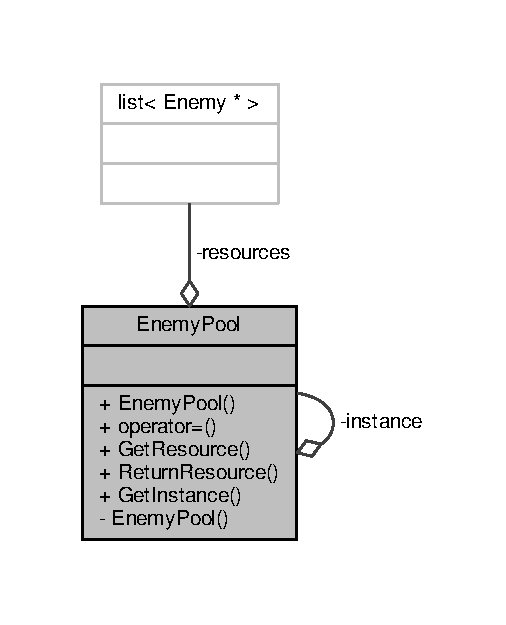
\includegraphics[width=243pt]{class_enemy_pool__coll__graph}
\end{center}
\end{figure}
\subsection*{Public Member Functions}
\begin{DoxyCompactItemize}
\item 
\hyperlink{class_enemy_pool_a7f7dfd08a6cb64c12c1f5842de977300}{Enemy\-Pool} (const \hyperlink{class_enemy_pool}{Enemy\-Pool} \&)=delete
\item 
\hyperlink{class_enemy_pool}{Enemy\-Pool} \& \hyperlink{class_enemy_pool_a9b652b5fdf0c284a4a6e6c51af66543c}{operator=} (const \hyperlink{class_enemy_pool}{Enemy\-Pool} \&)=delete
\item 
\hyperlink{class_enemy}{Enemy} $\ast$ \hyperlink{class_enemy_pool_ab2bf919b69de9b367aeeb231ad0b0b4e}{Get\-Resource} ()
\item 
void \hyperlink{class_enemy_pool_a23a38a606c719763861a882d9f5668e6}{Return\-Resource} (\hyperlink{class_enemy}{Enemy} $\ast$object)
\end{DoxyCompactItemize}
\subsection*{Static Public Member Functions}
\begin{DoxyCompactItemize}
\item 
static \hyperlink{class_enemy_pool}{Enemy\-Pool} $\ast$ \hyperlink{class_enemy_pool_a9a3e8badcf44d36e36e78d3bf008fd03}{Get\-Instance} (irr\-::\-Irrlicht\-Device $\ast$device)
\end{DoxyCompactItemize}
\subsection*{Private Member Functions}
\begin{DoxyCompactItemize}
\item 
\hyperlink{class_enemy_pool_a86c64cc1f5c0faeb1c78a6b602a2f5e6}{Enemy\-Pool} (irr\-::\-Irrlicht\-Device $\ast$device)
\end{DoxyCompactItemize}
\subsection*{Private Attributes}
\begin{DoxyCompactItemize}
\item 
std\-::list$<$ \hyperlink{class_enemy}{Enemy} $\ast$ $>$ \hyperlink{class_enemy_pool_a78b476ddede948197e107e8e594e25aa}{resources}
\end{DoxyCompactItemize}
\subsection*{Static Private Attributes}
\begin{DoxyCompactItemize}
\item 
static \hyperlink{class_enemy_pool}{Enemy\-Pool} $\ast$ \hyperlink{class_enemy_pool_aff307b55d5b5a8faf8023ee78c06c5e0}{instance} = 0
\end{DoxyCompactItemize}


\subsection{Constructor \& Destructor Documentation}
\hypertarget{class_enemy_pool_a7f7dfd08a6cb64c12c1f5842de977300}{\index{Enemy\-Pool@{Enemy\-Pool}!Enemy\-Pool@{Enemy\-Pool}}
\index{Enemy\-Pool@{Enemy\-Pool}!EnemyPool@{Enemy\-Pool}}
\subsubsection[{Enemy\-Pool}]{\setlength{\rightskip}{0pt plus 5cm}Enemy\-Pool\-::\-Enemy\-Pool (
\begin{DoxyParamCaption}
\item[{const {\bf Enemy\-Pool} \&}]{}
\end{DoxyParamCaption}
)\hspace{0.3cm}{\ttfamily [delete]}}}\label{class_enemy_pool_a7f7dfd08a6cb64c12c1f5842de977300}


Referenced by Get\-Instance().

\hypertarget{class_enemy_pool_a86c64cc1f5c0faeb1c78a6b602a2f5e6}{\index{Enemy\-Pool@{Enemy\-Pool}!Enemy\-Pool@{Enemy\-Pool}}
\index{Enemy\-Pool@{Enemy\-Pool}!EnemyPool@{Enemy\-Pool}}
\subsubsection[{Enemy\-Pool}]{\setlength{\rightskip}{0pt plus 5cm}Enemy\-Pool\-::\-Enemy\-Pool (
\begin{DoxyParamCaption}
\item[{irr\-::\-Irrlicht\-Device $\ast$}]{device}
\end{DoxyParamCaption}
)\hspace{0.3cm}{\ttfamily [private]}}}\label{class_enemy_pool_a86c64cc1f5c0faeb1c78a6b602a2f5e6}


References Enemy\-Pool\-Device.


\begin{DoxyCode}
7 \{
8     \hyperlink{_enemy_pool_8cpp_ad7774a435f9870c0a71f7d3d8d06bf94}{EnemyPoolDevice} = device;
9 \}
\end{DoxyCode}


\subsection{Member Function Documentation}
\hypertarget{class_enemy_pool_a9a3e8badcf44d36e36e78d3bf008fd03}{\index{Enemy\-Pool@{Enemy\-Pool}!Get\-Instance@{Get\-Instance}}
\index{Get\-Instance@{Get\-Instance}!EnemyPool@{Enemy\-Pool}}
\subsubsection[{Get\-Instance}]{\setlength{\rightskip}{0pt plus 5cm}{\bf Enemy\-Pool} $\ast$ Enemy\-Pool\-::\-Get\-Instance (
\begin{DoxyParamCaption}
\item[{irr\-::\-Irrlicht\-Device $\ast$}]{device}
\end{DoxyParamCaption}
)\hspace{0.3cm}{\ttfamily [static]}}}\label{class_enemy_pool_a9a3e8badcf44d36e36e78d3bf008fd03}


References Enemy\-Pool(), and instance.



Referenced by Enemy\-Spawner\-::\-Enemy\-Spawner().


\begin{DoxyCode}
14 \{
15     \textcolor{keywordflow}{if} (!\hyperlink{class_enemy_pool_aff307b55d5b5a8faf8023ee78c06c5e0}{instance})
16     \{
17         \hyperlink{class_enemy_pool_aff307b55d5b5a8faf8023ee78c06c5e0}{instance} = \textcolor{keyword}{new} \hyperlink{class_enemy_pool_a7f7dfd08a6cb64c12c1f5842de977300}{EnemyPool}(device);
18     \}
19     \textcolor{keywordflow}{return} \hyperlink{class_enemy_pool_aff307b55d5b5a8faf8023ee78c06c5e0}{instance};
20 \}
\end{DoxyCode}
\hypertarget{class_enemy_pool_ab2bf919b69de9b367aeeb231ad0b0b4e}{\index{Enemy\-Pool@{Enemy\-Pool}!Get\-Resource@{Get\-Resource}}
\index{Get\-Resource@{Get\-Resource}!EnemyPool@{Enemy\-Pool}}
\subsubsection[{Get\-Resource}]{\setlength{\rightskip}{0pt plus 5cm}{\bf Enemy} $\ast$ Enemy\-Pool\-::\-Get\-Resource (
\begin{DoxyParamCaption}
{}
\end{DoxyParamCaption}
)}}\label{class_enemy_pool_ab2bf919b69de9b367aeeb231ad0b0b4e}


References enemy, Enemy\-Pool\-Device, Enemy\-::\-Get\-Enemy\-Scene\-Node(), and resources.



Referenced by Enemy\-Spawner\-::\-Spawn(), and Enemy\-Spawner\-::\-Spawn\-Mathroska\-Minion().


\begin{DoxyCode}
23 \{
24     \textcolor{keywordflow}{if} (\hyperlink{class_enemy_pool_a78b476ddede948197e107e8e594e25aa}{resources}.empty())
25     \{
26         \hyperlink{class_enemy}{Enemy}* \hyperlink{_enemy_spawner_8cpp_acd5d4a5e84ef92e2e153fa20b425646f}{enemy} = \textcolor{keyword}{new} \hyperlink{class_enemy}{Enemy}(\hyperlink{_enemy_pool_8cpp_ad7774a435f9870c0a71f7d3d8d06bf94}{EnemyPoolDevice});
27         \textcolor{keywordflow}{return} \hyperlink{_enemy_spawner_8cpp_acd5d4a5e84ef92e2e153fa20b425646f}{enemy};
28     \}
29     \textcolor{keywordflow}{else}
30     \{
31         \hyperlink{class_enemy}{Enemy}* \hyperlink{_enemy_spawner_8cpp_acd5d4a5e84ef92e2e153fa20b425646f}{enemy} = \hyperlink{class_enemy_pool_a78b476ddede948197e107e8e594e25aa}{resources}.front();
32         \hyperlink{class_enemy_pool_a78b476ddede948197e107e8e594e25aa}{resources}.pop\_front();
33         enemy->\hyperlink{class_enemy_a85b8d7d8c6a61f8824a3b7b3fea795f4}{GetEnemySceneNode}()->setVisible(\textcolor{keyword}{true});
34         \textcolor{keywordflow}{return} \hyperlink{_enemy_spawner_8cpp_acd5d4a5e84ef92e2e153fa20b425646f}{enemy};
35     \}
36 \}
\end{DoxyCode}
\hypertarget{class_enemy_pool_a9b652b5fdf0c284a4a6e6c51af66543c}{\index{Enemy\-Pool@{Enemy\-Pool}!operator=@{operator=}}
\index{operator=@{operator=}!EnemyPool@{Enemy\-Pool}}
\subsubsection[{operator=}]{\setlength{\rightskip}{0pt plus 5cm}{\bf Enemy\-Pool}\& Enemy\-Pool\-::operator= (
\begin{DoxyParamCaption}
\item[{const {\bf Enemy\-Pool} \&}]{}
\end{DoxyParamCaption}
)\hspace{0.3cm}{\ttfamily [delete]}}}\label{class_enemy_pool_a9b652b5fdf0c284a4a6e6c51af66543c}
\hypertarget{class_enemy_pool_a23a38a606c719763861a882d9f5668e6}{\index{Enemy\-Pool@{Enemy\-Pool}!Return\-Resource@{Return\-Resource}}
\index{Return\-Resource@{Return\-Resource}!EnemyPool@{Enemy\-Pool}}
\subsubsection[{Return\-Resource}]{\setlength{\rightskip}{0pt plus 5cm}void Enemy\-Pool\-::\-Return\-Resource (
\begin{DoxyParamCaption}
\item[{{\bf Enemy} $\ast$}]{object}
\end{DoxyParamCaption}
)}}\label{class_enemy_pool_a23a38a606c719763861a882d9f5668e6}


References resources.



Referenced by Enemy\-Spawner\-::\-Update\-Enemies().


\begin{DoxyCode}
39 \{
40     \textcolor{keywordtype}{object}->Reset();
41     \hyperlink{class_enemy_pool_a78b476ddede948197e107e8e594e25aa}{resources}.push\_back(\textcolor{keywordtype}{object});
42 \}
\end{DoxyCode}


\subsection{Member Data Documentation}
\hypertarget{class_enemy_pool_aff307b55d5b5a8faf8023ee78c06c5e0}{\index{Enemy\-Pool@{Enemy\-Pool}!instance@{instance}}
\index{instance@{instance}!EnemyPool@{Enemy\-Pool}}
\subsubsection[{instance}]{\setlength{\rightskip}{0pt plus 5cm}{\bf Enemy\-Pool} $\ast$ Enemy\-Pool\-::instance = 0\hspace{0.3cm}{\ttfamily [static]}, {\ttfamily [private]}}}\label{class_enemy_pool_aff307b55d5b5a8faf8023ee78c06c5e0}


Referenced by Get\-Instance().

\hypertarget{class_enemy_pool_a78b476ddede948197e107e8e594e25aa}{\index{Enemy\-Pool@{Enemy\-Pool}!resources@{resources}}
\index{resources@{resources}!EnemyPool@{Enemy\-Pool}}
\subsubsection[{resources}]{\setlength{\rightskip}{0pt plus 5cm}std\-::list$<${\bf Enemy}$\ast$$>$ Enemy\-Pool\-::resources\hspace{0.3cm}{\ttfamily [private]}}}\label{class_enemy_pool_a78b476ddede948197e107e8e594e25aa}


Referenced by Get\-Resource(), and Return\-Resource().



The documentation for this class was generated from the following files\-:\begin{DoxyCompactItemize}
\item 
\hyperlink{_enemy_pool_8h}{Enemy\-Pool.\-h}\item 
\hyperlink{_enemy_pool_8cpp}{Enemy\-Pool.\-cpp}\end{DoxyCompactItemize}

\hypertarget{class_enemy_spawner}{\section{Enemy\-Spawner Class Reference}
\label{class_enemy_spawner}\index{Enemy\-Spawner@{Enemy\-Spawner}}
}


{\ttfamily \#include $<$Enemy\-Spawner.\-h$>$}



Collaboration diagram for Enemy\-Spawner\-:
\nopagebreak
\begin{figure}[H]
\begin{center}
\leavevmode
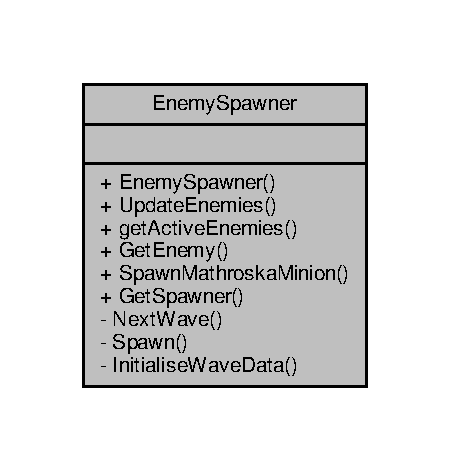
\includegraphics[width=216pt]{class_enemy_spawner__coll__graph}
\end{center}
\end{figure}
\subsection*{Public Member Functions}
\begin{DoxyCompactItemize}
\item 
\hyperlink{class_enemy_spawner_a3553ec74e00d89f89f323b36cc9bf3f6}{Enemy\-Spawner} (irr\-::\-Irrlicht\-Device $\ast$device, \hyperlink{class_player}{Player} $\ast$\hyperlink{_enemy_8cpp_a96781128d3743da3d17e0fdd91afba7b}{player})
\item 
void \hyperlink{class_enemy_spawner_ab7717d2d42a40b943564629a85f0fabc}{Update\-Enemies} ()
\item 
irr\-::core\-::array$<$ \hyperlink{class_enemy}{Enemy} $\ast$ $>$ \hyperlink{class_enemy_spawner_ad83b7b7bfe4904e9addcad621d62295d}{get\-Active\-Enemies} ()
\item 
\hyperlink{class_enemy}{Enemy} $\ast$ \hyperlink{class_enemy_spawner_a42d5341193911135909c3df1a6271d3f}{Get\-Enemy} (int id)
\item 
void \hyperlink{class_enemy_spawner_ac664064f5f057837fde5c2e81daa2e6e}{Spawn\-Mathroska\-Minion} (irr\-::core\-::vector3df spawn\-Pos, \hyperlink{class_enemy_a98c2ee2c2081001de17a4bc9fa8da94f}{Enemy\-::\-Enemy\-Type} enemy\-Type, irr\-::s32 nest\-Amount=0)
\end{DoxyCompactItemize}
\subsection*{Static Public Member Functions}
\begin{DoxyCompactItemize}
\item 
static \hyperlink{class_enemy_spawner}{Enemy\-Spawner} $\ast$ \hyperlink{class_enemy_spawner_a9a7a1adc56f040fd2c139a6acdae0d90}{Get\-Spawner} ()
\end{DoxyCompactItemize}
\subsection*{Private Member Functions}
\begin{DoxyCompactItemize}
\item 
void \hyperlink{class_enemy_spawner_ad7105663a68f8cb931af64463f0286c8}{Next\-Wave} ()
\item 
void \hyperlink{class_enemy_spawner_a047cc9ff180ef6bb4a1cc437b786553b}{Spawn} ()
\item 
void \hyperlink{class_enemy_spawner_a42f58b89cfdfd21a19459d850a79876d}{Initialise\-Wave\-Data} ()
\end{DoxyCompactItemize}


\subsection{Constructor \& Destructor Documentation}
\hypertarget{class_enemy_spawner_a3553ec74e00d89f89f323b36cc9bf3f6}{\index{Enemy\-Spawner@{Enemy\-Spawner}!Enemy\-Spawner@{Enemy\-Spawner}}
\index{Enemy\-Spawner@{Enemy\-Spawner}!EnemySpawner@{Enemy\-Spawner}}
\subsubsection[{Enemy\-Spawner}]{\setlength{\rightskip}{0pt plus 5cm}Enemy\-Spawner\-::\-Enemy\-Spawner (
\begin{DoxyParamCaption}
\item[{irr\-::\-Irrlicht\-Device $\ast$}]{device, }
\item[{{\bf Player} $\ast$}]{player}
\end{DoxyParamCaption}
)}}\label{class_enemy_spawner_a3553ec74e00d89f89f323b36cc9bf3f6}


References \-\_\-cam, \-\_\-player, amount\-Of\-Enemies, enem\-Spawn\-Sound\-Manager, enemy\-Pool, enemy\-Spawner\-I\-Device, enemy\-Spawner\-Smgr, game\-\_\-\-Enemy\-Spawner, Enemy\-Pool\-::\-Get\-Instance(), Game\-::\-Get\-Instance(), Sound\-Manager\-::\-Get\-Instance(), Heat\-Map\-Manager\-::\-Get\-Instance(), Camera\-::\-Get\-Instance(), heat\-Map\-Mngr, particle\-System, prev\-Frame\-Time, resize, spawner, and spawn\-Positions.


\begin{DoxyCode}
62 \{
63     \hyperlink{_enemy_spawner_8cpp_a351bdd6d08cc3965554b639f8e11e360}{particleSystem} = \textcolor{keyword}{new} \hyperlink{class_particle_system}{ParticleSystem}(device);
64     \hyperlink{_enemy_spawner_8cpp_a6fb6c47d7964fa1186985510e544e686}{enemySpawnerIDevice} = device;
65     \hyperlink{_enemy_spawner_8cpp_acdc4e203d85a9683181751a7695ee478}{enemySpawnerSmgr} = \hyperlink{_enemy_spawner_8cpp_a6fb6c47d7964fa1186985510e544e686}{enemySpawnerIDevice}->getSceneManager();
66     \hyperlink{_enemy_spawner_8cpp_a9cd078164ceb4e9bfed2981b94610dc9}{\_player} = \hyperlink{class_player}{Player};
67     \hyperlink{_enemy_spawner_8cpp_a473330ef228d901a0124176f437f5855}{game\_EnemySpawner} = \hyperlink{_enemy_spawner_8cpp_a473330ef228d901a0124176f437f5855}{game\_EnemySpawner}->
      \hyperlink{class_game_aa989d3cee96d5ae093663bf62dea57e2}{GetInstance}();
68     \hyperlink{_enemy_spawner_8cpp_a4dcc017b886f43aae8dec561367a6d3c}{heatMapMngr} = \hyperlink{_enemy_spawner_8cpp_a4dcc017b886f43aae8dec561367a6d3c}{heatMapMngr}->\hyperlink{class_heat_map_manager_acc2cf6cbce0774a997ef1c408f07fb87}{GetInstance}();
69     \hyperlink{_enemy_spawner_8cpp_a10a9f0b14afa27bb442d05b6a40464d6}{enemyPool} = \hyperlink{class_enemy_pool_a9a3e8badcf44d36e36e78d3bf008fd03}{EnemyPool::GetInstance}(device);
70     \hyperlink{_enemy_spawner_8cpp_af02f2a517a39d70a0afb3929737a472c}{\_cam} = \hyperlink{_enemy_spawner_8cpp_af02f2a517a39d70a0afb3929737a472c}{\_cam}->\hyperlink{class_camera_aae2256f0ee62dd982d92c09d9d00c8d5}{GetInstance}(NULL);
71     \hyperlink{_enemy_spawner_8cpp_a8be9978ac9406d024ff2aaf7c719b8cd}{amountOfEnemies} = 12;
72     \hyperlink{_enemy_spawner_8cpp_a23cc32f539e1b8c74174c581008b5546}{resize} = 2;
73     \hyperlink{_enemy_spawner_8cpp_a3bdc7599b0df4bac902695a10b091f2f}{enemSpawnSoundManager} = \hyperlink{_enemy_spawner_8cpp_a3bdc7599b0df4bac902695a10b091f2f}{enemSpawnSoundManager}->
      \hyperlink{class_sound_manager_a887480b38c9380c9fba23a2337df63be}{GetInstance}();
74     \textcolor{comment}{//setting spawnpositions in the corners.}
75     \hyperlink{_enemy_spawner_8cpp_a309ce9c456c1040e752ba1a54dcd85a5}{spawnPositions}.push\_back(vector3df(-82, 0, -78) * \hyperlink{_enemy_spawner_8cpp_a23cc32f539e1b8c74174c581008b5546}{resize});
76     \hyperlink{_enemy_spawner_8cpp_a309ce9c456c1040e752ba1a54dcd85a5}{spawnPositions}.push\_back(vector3df(78, 0, -78) * \hyperlink{_enemy_spawner_8cpp_a23cc32f539e1b8c74174c581008b5546}{resize});
77     \hyperlink{_enemy_spawner_8cpp_a309ce9c456c1040e752ba1a54dcd85a5}{spawnPositions}.push\_back(vector3df(78, 0, 78) * \hyperlink{_enemy_spawner_8cpp_a23cc32f539e1b8c74174c581008b5546}{resize});
78     \hyperlink{_enemy_spawner_8cpp_a309ce9c456c1040e752ba1a54dcd85a5}{spawnPositions}.push\_back(vector3df(-82, 0, 78) * \hyperlink{_enemy_spawner_8cpp_a23cc32f539e1b8c74174c581008b5546}{resize});
79 
80     \textcolor{comment}{// In order to do framerate independent movement, we have to know}
81     \textcolor{comment}{// how long it was since the last frame}
82     \hyperlink{_enemy_spawner_8cpp_a7f39b7d91ba9b2a31bad8f8558b8a0d9}{prevFrameTime} = \hyperlink{_enemy_spawner_8cpp_a6fb6c47d7964fa1186985510e544e686}{enemySpawnerIDevice}->getTimer()->getTime();
83     \hyperlink{class_enemy_spawner_a42f58b89cfdfd21a19459d850a79876d}{InitialiseWaveData}();
84     \hyperlink{_enemy_spawner_8cpp_a665825e12de83fe61e6d661d5ae65c3b}{spawner} = \textcolor{keyword}{this};
85 
86     \hyperlink{class_enemy_spawner_a047cc9ff180ef6bb4a1cc437b786553b}{Spawn}();
87 \}
\end{DoxyCode}


\subsection{Member Function Documentation}
\hypertarget{class_enemy_spawner_ad83b7b7bfe4904e9addcad621d62295d}{\index{Enemy\-Spawner@{Enemy\-Spawner}!get\-Active\-Enemies@{get\-Active\-Enemies}}
\index{get\-Active\-Enemies@{get\-Active\-Enemies}!EnemySpawner@{Enemy\-Spawner}}
\subsubsection[{get\-Active\-Enemies}]{\setlength{\rightskip}{0pt plus 5cm}core\-::array$<$ {\bf Enemy} $\ast$ $>$ Enemy\-Spawner\-::get\-Active\-Enemies (
\begin{DoxyParamCaption}
{}
\end{DoxyParamCaption}
)}}\label{class_enemy_spawner_ad83b7b7bfe4904e9addcad621d62295d}


References active\-Enemies.



Referenced by Player\-::\-Shoot().


\begin{DoxyCode}
187 \{ \textcolor{keywordflow}{return} \hyperlink{_enemy_spawner_8cpp_a3d9bb20c5ed03047464ed534dc3938ba}{activeEnemies}; \}
\end{DoxyCode}
\hypertarget{class_enemy_spawner_a42d5341193911135909c3df1a6271d3f}{\index{Enemy\-Spawner@{Enemy\-Spawner}!Get\-Enemy@{Get\-Enemy}}
\index{Get\-Enemy@{Get\-Enemy}!EnemySpawner@{Enemy\-Spawner}}
\subsubsection[{Get\-Enemy}]{\setlength{\rightskip}{0pt plus 5cm}{\bf Enemy} $\ast$ Enemy\-Spawner\-::\-Get\-Enemy (
\begin{DoxyParamCaption}
\item[{int}]{id}
\end{DoxyParamCaption}
)}}\label{class_enemy_spawner_a42d5341193911135909c3df1a6271d3f}


References active\-Enemies.



Referenced by Player\-::\-Shoot().


\begin{DoxyCode}
188 \{ \textcolor{keywordflow}{return} \hyperlink{_enemy_spawner_8cpp_a3d9bb20c5ed03047464ed534dc3938ba}{activeEnemies}[id]; \}
\end{DoxyCode}
\hypertarget{class_enemy_spawner_a9a7a1adc56f040fd2c139a6acdae0d90}{\index{Enemy\-Spawner@{Enemy\-Spawner}!Get\-Spawner@{Get\-Spawner}}
\index{Get\-Spawner@{Get\-Spawner}!EnemySpawner@{Enemy\-Spawner}}
\subsubsection[{Get\-Spawner}]{\setlength{\rightskip}{0pt plus 5cm}{\bf Enemy\-Spawner} $\ast$ Enemy\-Spawner\-::\-Get\-Spawner (
\begin{DoxyParamCaption}
{}
\end{DoxyParamCaption}
)\hspace{0.3cm}{\ttfamily [static]}}}\label{class_enemy_spawner_a9a7a1adc56f040fd2c139a6acdae0d90}


References spawner.



Referenced by Enemy\-::\-Take\-Damage().


\begin{DoxyCode}
189 \{ \textcolor{keywordflow}{return} \hyperlink{_enemy_spawner_8cpp_a665825e12de83fe61e6d661d5ae65c3b}{spawner}; \}
\end{DoxyCode}
\hypertarget{class_enemy_spawner_a42f58b89cfdfd21a19459d850a79876d}{\index{Enemy\-Spawner@{Enemy\-Spawner}!Initialise\-Wave\-Data@{Initialise\-Wave\-Data}}
\index{Initialise\-Wave\-Data@{Initialise\-Wave\-Data}!EnemySpawner@{Enemy\-Spawner}}
\subsubsection[{Initialise\-Wave\-Data}]{\setlength{\rightskip}{0pt plus 5cm}void Enemy\-Spawner\-::\-Initialise\-Wave\-Data (
\begin{DoxyParamCaption}
{}
\end{DoxyParamCaption}
)\hspace{0.3cm}{\ttfamily [private]}}}\label{class_enemy_spawner_a42f58b89cfdfd21a19459d850a79876d}


References wave\-Data.


\begin{DoxyCode}
192 \{
193     \textcolor{comment}{//Amount of enemies:}
194     \hyperlink{_enemy_spawner_8cpp_a1b5d1dbce59dba7751cd9feaa3a2c40b}{waveData}[0] = \textcolor{keyword}{new} \hyperlink{struct_wave_data}{WaveData}(0, 0, 0, 0, 0);\textcolor{comment}{//5}
195     \hyperlink{_enemy_spawner_8cpp_a1b5d1dbce59dba7751cd9feaa3a2c40b}{waveData}[1] = \textcolor{keyword}{new} \hyperlink{struct_wave_data}{WaveData}(1, 5, 0, 0, 0);\textcolor{comment}{//5}
196     \hyperlink{_enemy_spawner_8cpp_a1b5d1dbce59dba7751cd9feaa3a2c40b}{waveData}[2] = \textcolor{keyword}{new} \hyperlink{struct_wave_data}{WaveData}(2, 10, 0, 0, 0);\textcolor{comment}{//10}
197     \hyperlink{_enemy_spawner_8cpp_a1b5d1dbce59dba7751cd9feaa3a2c40b}{waveData}[3] = \textcolor{keyword}{new} \hyperlink{struct_wave_data}{WaveData}(3, 8, 3, 0, 0);\textcolor{comment}{//11}
198     \hyperlink{_enemy_spawner_8cpp_a1b5d1dbce59dba7751cd9feaa3a2c40b}{waveData}[4] = \textcolor{keyword}{new} \hyperlink{struct_wave_data}{WaveData}(4, 12, 5, 0, 0);\textcolor{comment}{//17}
199     \hyperlink{_enemy_spawner_8cpp_a1b5d1dbce59dba7751cd9feaa3a2c40b}{waveData}[5] = \textcolor{keyword}{new} \hyperlink{struct_wave_data}{WaveData}(5, 15, 2, 2, 2);\textcolor{comment}{//20}
200     \hyperlink{_enemy_spawner_8cpp_a1b5d1dbce59dba7751cd9feaa3a2c40b}{waveData}[6] = \textcolor{keyword}{new} \hyperlink{struct_wave_data}{WaveData}(6, 10, 0, 7, 2);\textcolor{comment}{//18}
201     \hyperlink{_enemy_spawner_8cpp_a1b5d1dbce59dba7751cd9feaa3a2c40b}{waveData}[7] = \textcolor{keyword}{new} \hyperlink{struct_wave_data}{WaveData}(7, 7, 7, 4, 2); \textcolor{comment}{//20}
202     \hyperlink{_enemy_spawner_8cpp_a1b5d1dbce59dba7751cd9feaa3a2c40b}{waveData}[8] = \textcolor{keyword}{new} \hyperlink{struct_wave_data}{WaveData}(8, 0, 15, 0, 5); \textcolor{comment}{//20}
203     \hyperlink{_enemy_spawner_8cpp_a1b5d1dbce59dba7751cd9feaa3a2c40b}{waveData}[9] = \textcolor{keyword}{new} \hyperlink{struct_wave_data}{WaveData}(9, 0, 0, 15, 7); \textcolor{comment}{//22}
204     \hyperlink{_enemy_spawner_8cpp_a1b5d1dbce59dba7751cd9feaa3a2c40b}{waveData}[10] = \textcolor{keyword}{new} \hyperlink{struct_wave_data}{WaveData}(10, 10, 10, 10, 8); \textcolor{comment}{//38}
205     \hyperlink{_enemy_spawner_8cpp_a1b5d1dbce59dba7751cd9feaa3a2c40b}{waveData}[11] = \textcolor{keyword}{new} \hyperlink{struct_wave_data}{WaveData}(11, 0, 15, 15, 10); \textcolor{comment}{//40}
206     \hyperlink{_enemy_spawner_8cpp_a1b5d1dbce59dba7751cd9feaa3a2c40b}{waveData}[12] = \textcolor{keyword}{new} \hyperlink{struct_wave_data}{WaveData}(12, 10, 10, 10, 10); \textcolor{comment}{//40}
207     \hyperlink{_enemy_spawner_8cpp_a1b5d1dbce59dba7751cd9feaa3a2c40b}{waveData}[13] = \textcolor{keyword}{new} \hyperlink{struct_wave_data}{WaveData}(13, 15, 15, 15, 15); \textcolor{comment}{//40}
208     \hyperlink{_enemy_spawner_8cpp_a1b5d1dbce59dba7751cd9feaa3a2c40b}{waveData}[14] = \textcolor{keyword}{new} \hyperlink{struct_wave_data}{WaveData}(14, 20, 20, 20, 20); \textcolor{comment}{//40}
209 \}
\end{DoxyCode}
\hypertarget{class_enemy_spawner_ad7105663a68f8cb931af64463f0286c8}{\index{Enemy\-Spawner@{Enemy\-Spawner}!Next\-Wave@{Next\-Wave}}
\index{Next\-Wave@{Next\-Wave}!EnemySpawner@{Enemy\-Spawner}}
\subsubsection[{Next\-Wave}]{\setlength{\rightskip}{0pt plus 5cm}void Enemy\-Spawner\-::\-Next\-Wave (
\begin{DoxyParamCaption}
{}
\end{DoxyParamCaption}
)\hspace{0.3cm}{\ttfamily [private]}}}\label{class_enemy_spawner_ad7105663a68f8cb931af64463f0286c8}


References \-\_\-cam, B\-I\-G\-\_\-\-W\-A\-V\-E\-\_\-\-I\-N\-C\-O\-M\-I\-N\-G\-\_\-\-S\-O\-U\-N\-D, Camera\-::big\-Wave\-Shaking, current\-Time, current\-Wave, enem\-Spawn\-Sound\-Manager, enemy\-Spawner\-I\-Device, max\-Wave\-Cooldown, new\-Wave, Sound\-Manager\-::\-Play\-Sound(), Camera\-::state, W\-A\-V\-E\-\_\-\-I\-N\-C\-O\-M\-I\-N\-G\-\_\-\-S\-O\-U\-N\-D, wave\-Change\-U\-I, wave\-Cooldown, Camera\-::wave\-Shaking, and wave\-Timer\-Set.


\begin{DoxyCode}
147 \{
148     \textcolor{keyword}{const} u32 now\_ = \hyperlink{_enemy_spawner_8cpp_a6fb6c47d7964fa1186985510e544e686}{enemySpawnerIDevice}->getTimer()->getTime();
149     \textcolor{keyword}{const} f32 frameTime = (f32)(now\_ - \hyperlink{_enemy_spawner_8cpp_a9b0eac166daf4ddfb21d451eb574aca3}{currentTime}) / 1000.f; \textcolor{comment}{// Time in seconds}
150     \hyperlink{_enemy_spawner_8cpp_a9b0eac166daf4ddfb21d451eb574aca3}{currentTime} = now\_;
151 
152     \textcolor{keywordflow}{if} (\hyperlink{_enemy_spawner_8cpp_aa4f3458458a5f172e5b160fb68473d97}{waveTimerSet} == \textcolor{keyword}{false} && \hyperlink{_enemy_spawner_8cpp_a72775aa668ffb2a0d7e469173cdd5b93}{waveCooldown} > 0)
153     \{
154         \textcolor{keywordflow}{if} (\hyperlink{_enemy_spawner_8cpp_abccd7907e4faa3f04b4a786d64599f8e}{newWave}) 
155         \{
156             \textcolor{keywordflow}{if} ((\hyperlink{_enemy_spawner_8cpp_ae8875f134fe6fadbb9f14c149ef06d50}{currentWave} + 1) % 5 == 0)
157                 \hyperlink{_enemy_spawner_8cpp_a3bdc7599b0df4bac902695a10b091f2f}{enemSpawnSoundManager}->\hyperlink{class_sound_manager_a81e8f88fe549f6767d3552f12c28ecbc}{PlaySound}(
      \hyperlink{_enemy_spawner_8cpp_aea6158bfc7b897c6c2f1fcf801da1883}{BIG\_WAVE\_INCOMING\_SOUND}, \textcolor{keyword}{false});
158             \textcolor{keywordflow}{else}
159                 \hyperlink{_enemy_spawner_8cpp_a3bdc7599b0df4bac902695a10b091f2f}{enemSpawnSoundManager}->\hyperlink{class_sound_manager_a81e8f88fe549f6767d3552f12c28ecbc}{PlaySound}(
      \hyperlink{_enemy_spawner_8cpp_a4a8c0d8fc8a70f796d700f01c8a9021a}{WAVE\_INCOMING\_SOUND}, \textcolor{keyword}{false});
160 
161             \hyperlink{_enemy_spawner_8cpp_abccd7907e4faa3f04b4a786d64599f8e}{newWave} = \textcolor{keyword}{false};
162         \}
163         \hyperlink{_enemy_spawner_8cpp_a30a29af809eac59191fdd00041d88039}{waveChangeUI} = \textcolor{keyword}{true};
164         \hyperlink{_enemy_spawner_8cpp_a72775aa668ffb2a0d7e469173cdd5b93}{waveCooldown} -= frameTime;
165         \textcolor{keywordflow}{if} (\hyperlink{_enemy_spawner_8cpp_a72775aa668ffb2a0d7e469173cdd5b93}{waveCooldown} <= 0)
166         \{
167             \hyperlink{_enemy_spawner_8cpp_ae8875f134fe6fadbb9f14c149ef06d50}{currentWave}++;
168             \hyperlink{class_enemy_spawner_a047cc9ff180ef6bb4a1cc437b786553b}{Spawn}();
169             \textcolor{keywordflow}{if} (\hyperlink{_enemy_spawner_8cpp_ae8875f134fe6fadbb9f14c149ef06d50}{currentWave} % 5 == 0)
170             \{
171                 \hyperlink{_enemy_spawner_8cpp_af02f2a517a39d70a0afb3929737a472c}{\_cam}->\hyperlink{class_camera_a87960570c2d28bd4471c5a74fc021cb5}{state} = \hyperlink{_enemy_spawner_8cpp_af02f2a517a39d70a0afb3929737a472c}{\_cam}->\hyperlink{class_camera_a1ddf5d726e6c1d1d1c08d96d42c40236a3a50c28c61cd1a7f837b32c54a65c92d}{bigWaveShaking};
172                 \hyperlink{_enemy_spawner_8cpp_abccd7907e4faa3f04b4a786d64599f8e}{newWave} = \textcolor{keyword}{true};
173             \}
174             \textcolor{keywordflow}{else}
175             \{
176                 \hyperlink{_enemy_spawner_8cpp_af02f2a517a39d70a0afb3929737a472c}{\_cam}->\hyperlink{class_camera_a87960570c2d28bd4471c5a74fc021cb5}{state} = \hyperlink{_enemy_spawner_8cpp_af02f2a517a39d70a0afb3929737a472c}{\_cam}->\hyperlink{class_camera_a1ddf5d726e6c1d1d1c08d96d42c40236a9bb1793c9685b74a790ea306a7852179}{waveShaking};
177                 \hyperlink{_enemy_spawner_8cpp_abccd7907e4faa3f04b4a786d64599f8e}{newWave} = \textcolor{keyword}{true};
178             \}
179             \textcolor{comment}{//Insert pause/UI between waves here}
180             \hyperlink{_enemy_spawner_8cpp_aa4f3458458a5f172e5b160fb68473d97}{waveTimerSet} = \textcolor{keyword}{true};
181             \hyperlink{_enemy_spawner_8cpp_a72775aa668ffb2a0d7e469173cdd5b93}{waveCooldown} = \hyperlink{_enemy_spawner_8cpp_aae252475624f4edf5c9353f3eb15532d}{maxWaveCooldown};
182             \hyperlink{_enemy_spawner_8cpp_a30a29af809eac59191fdd00041d88039}{waveChangeUI} = \textcolor{keyword}{false};
183             \hyperlink{_enemy_spawner_8cpp_aa4f3458458a5f172e5b160fb68473d97}{waveTimerSet} = \textcolor{keyword}{false};
184         \}
185     \}
186 \}
\end{DoxyCode}
\hypertarget{class_enemy_spawner_a047cc9ff180ef6bb4a1cc437b786553b}{\index{Enemy\-Spawner@{Enemy\-Spawner}!Spawn@{Spawn}}
\index{Spawn@{Spawn}!EnemySpawner@{Enemy\-Spawner}}
\subsubsection[{Spawn}]{\setlength{\rightskip}{0pt plus 5cm}void Enemy\-Spawner\-::\-Spawn (
\begin{DoxyParamCaption}
{}
\end{DoxyParamCaption}
)\hspace{0.3cm}{\ttfamily [private]}}}\label{class_enemy_spawner_a047cc9ff180ef6bb4a1cc437b786553b}


References \-\_\-player, active\-Enemies, Collision\-::\-Add\-Dynamic\-To\-List(), collision, current\-Wave, enemy, enemy\-Pool, Enemy\-::\-Get\-Enemy\-Scene\-Node(), Enemy\-Pool\-::\-Get\-Resource(), Wave\-Data\-::max\-Fast\-Enem, Wave\-Data\-::max\-Matro\-Enem, Wave\-Data\-::max\-Regular\-Enem, Wave\-Data\-::max\-Tank\-Enem, Enemy\-::\-Set\-Enemy\-Type(), Enemy\-::\-Set\-Player(), spawn\-Positions, time, and wave\-Data.


\begin{DoxyCode}
221 \{
222     \textcolor{keywordflow}{for} (\textcolor{keywordtype}{int} i = 0; i < \hyperlink{_enemy_spawner_8cpp_a1b5d1dbce59dba7751cd9feaa3a2c40b}{waveData}[\hyperlink{_enemy_spawner_8cpp_ae8875f134fe6fadbb9f14c149ef06d50}{currentWave}]->\hyperlink{struct_wave_data_a70b7b4b2a611aa961b4f7c7bbbbcafcb}{maxRegularEnem}; i++)
223     \{
224         srand(\hyperlink{_player_8cpp_ab683520676b99a7bcc7a6299eb886247}{time}(NULL) * i);
225         u32 randomPos = rand() % 4;
226 
227         \hyperlink{_enemy_spawner_8cpp_acd5d4a5e84ef92e2e153fa20b425646f}{enemy} = \hyperlink{_enemy_spawner_8cpp_a10a9f0b14afa27bb442d05b6a40464d6}{enemyPool}->\hyperlink{class_enemy_pool_ab2bf919b69de9b367aeeb231ad0b0b4e}{GetResource}();
228         \hyperlink{_enemy_spawner_8cpp_acd5d4a5e84ef92e2e153fa20b425646f}{enemy}->\hyperlink{class_enemy_a421d67f70801a3399ca22067fcde6dff}{SetPlayer}(\hyperlink{_enemy_spawner_8cpp_a9cd078164ceb4e9bfed2981b94610dc9}{\_player});
229         \hyperlink{_enemy_spawner_8cpp_acd5d4a5e84ef92e2e153fa20b425646f}{enemy}->\hyperlink{class_enemy_a567a82f1d7cb9034509459850f7784fc}{SetEnemyType}(Enemy::EnemyType::basic);
230         \hyperlink{_enemy_spawner_8cpp_acd5d4a5e84ef92e2e153fa20b425646f}{enemy}->\hyperlink{class_enemy_a85b8d7d8c6a61f8824a3b7b3fea795f4}{GetEnemySceneNode}()->setPosition(
      \hyperlink{_enemy_spawner_8cpp_a309ce9c456c1040e752ba1a54dcd85a5}{spawnPositions}[randomPos]);
231         \hyperlink{_enemy_spawner_8cpp_abb03345f36a95239d14eaf664bf1c8cc}{collision}.\hyperlink{class_collision_a48551c4c00be185dc16cf27775bd177b}{AddDynamicToList}(\hyperlink{_enemy_spawner_8cpp_acd5d4a5e84ef92e2e153fa20b425646f}{enemy}->
      \hyperlink{class_enemy_a85b8d7d8c6a61f8824a3b7b3fea795f4}{GetEnemySceneNode}());
232         \hyperlink{_enemy_spawner_8cpp_a3d9bb20c5ed03047464ed534dc3938ba}{activeEnemies}.push\_back(\hyperlink{_enemy_spawner_8cpp_acd5d4a5e84ef92e2e153fa20b425646f}{enemy});
233     \}
234 
235     \textcolor{keywordflow}{for} (\textcolor{keywordtype}{int} j = 0; j < \hyperlink{_enemy_spawner_8cpp_a1b5d1dbce59dba7751cd9feaa3a2c40b}{waveData}[\hyperlink{_enemy_spawner_8cpp_ae8875f134fe6fadbb9f14c149ef06d50}{currentWave}]->\hyperlink{struct_wave_data_a730aa951bab558b2a39ab8cad3e0c6b0}{maxFastEnem}; j++)
236     \{
237         srand(\hyperlink{_player_8cpp_ab683520676b99a7bcc7a6299eb886247}{time}(NULL) * j);
238         u32 randomPos = rand() % 4;
239 
240         \hyperlink{_enemy_spawner_8cpp_acd5d4a5e84ef92e2e153fa20b425646f}{enemy} = \hyperlink{_enemy_spawner_8cpp_a10a9f0b14afa27bb442d05b6a40464d6}{enemyPool}->\hyperlink{class_enemy_pool_ab2bf919b69de9b367aeeb231ad0b0b4e}{GetResource}();
241         \hyperlink{_enemy_spawner_8cpp_acd5d4a5e84ef92e2e153fa20b425646f}{enemy}->\hyperlink{class_enemy_a421d67f70801a3399ca22067fcde6dff}{SetPlayer}(\hyperlink{_enemy_spawner_8cpp_a9cd078164ceb4e9bfed2981b94610dc9}{\_player});
242         \hyperlink{_enemy_spawner_8cpp_acd5d4a5e84ef92e2e153fa20b425646f}{enemy}->\hyperlink{class_enemy_a567a82f1d7cb9034509459850f7784fc}{SetEnemyType}(Enemy::EnemyType::fast);
243         \hyperlink{_enemy_spawner_8cpp_acd5d4a5e84ef92e2e153fa20b425646f}{enemy}->\hyperlink{class_enemy_a85b8d7d8c6a61f8824a3b7b3fea795f4}{GetEnemySceneNode}()->setPosition(
      \hyperlink{_enemy_spawner_8cpp_a309ce9c456c1040e752ba1a54dcd85a5}{spawnPositions}[randomPos]);
244         \hyperlink{_enemy_spawner_8cpp_abb03345f36a95239d14eaf664bf1c8cc}{collision}.\hyperlink{class_collision_a48551c4c00be185dc16cf27775bd177b}{AddDynamicToList}(\hyperlink{_enemy_spawner_8cpp_acd5d4a5e84ef92e2e153fa20b425646f}{enemy}->
      \hyperlink{class_enemy_a85b8d7d8c6a61f8824a3b7b3fea795f4}{GetEnemySceneNode}());
245         \hyperlink{_enemy_spawner_8cpp_a3d9bb20c5ed03047464ed534dc3938ba}{activeEnemies}.push\_back(\hyperlink{_enemy_spawner_8cpp_acd5d4a5e84ef92e2e153fa20b425646f}{enemy});
246     \}
247 
248     \textcolor{keywordflow}{for} (\textcolor{keywordtype}{int} k = 0; k < \hyperlink{_enemy_spawner_8cpp_a1b5d1dbce59dba7751cd9feaa3a2c40b}{waveData}[\hyperlink{_enemy_spawner_8cpp_ae8875f134fe6fadbb9f14c149ef06d50}{currentWave}]->\hyperlink{struct_wave_data_a85236ef7a2ac44e7364c65e106a341da}{maxTankEnem}; k++)
249     \{
250         srand(\hyperlink{_player_8cpp_ab683520676b99a7bcc7a6299eb886247}{time}(NULL) * k);
251         u32 randomPos = rand() % 4;
252 
253         \hyperlink{_enemy_spawner_8cpp_acd5d4a5e84ef92e2e153fa20b425646f}{enemy} = \hyperlink{_enemy_spawner_8cpp_a10a9f0b14afa27bb442d05b6a40464d6}{enemyPool}->\hyperlink{class_enemy_pool_ab2bf919b69de9b367aeeb231ad0b0b4e}{GetResource}();
254         \hyperlink{_enemy_spawner_8cpp_acd5d4a5e84ef92e2e153fa20b425646f}{enemy}->\hyperlink{class_enemy_a421d67f70801a3399ca22067fcde6dff}{SetPlayer}(\hyperlink{_enemy_spawner_8cpp_a9cd078164ceb4e9bfed2981b94610dc9}{\_player});
255         \hyperlink{_enemy_spawner_8cpp_acd5d4a5e84ef92e2e153fa20b425646f}{enemy}->\hyperlink{class_enemy_a567a82f1d7cb9034509459850f7784fc}{SetEnemyType}(Enemy::EnemyType::tanky);
256         \hyperlink{_enemy_spawner_8cpp_acd5d4a5e84ef92e2e153fa20b425646f}{enemy}->\hyperlink{class_enemy_a85b8d7d8c6a61f8824a3b7b3fea795f4}{GetEnemySceneNode}()->setPosition(
      \hyperlink{_enemy_spawner_8cpp_a309ce9c456c1040e752ba1a54dcd85a5}{spawnPositions}[randomPos]);
257         \hyperlink{_enemy_spawner_8cpp_abb03345f36a95239d14eaf664bf1c8cc}{collision}.\hyperlink{class_collision_a48551c4c00be185dc16cf27775bd177b}{AddDynamicToList}(\hyperlink{_enemy_spawner_8cpp_acd5d4a5e84ef92e2e153fa20b425646f}{enemy}->
      \hyperlink{class_enemy_a85b8d7d8c6a61f8824a3b7b3fea795f4}{GetEnemySceneNode}());
258         \hyperlink{_enemy_spawner_8cpp_a3d9bb20c5ed03047464ed534dc3938ba}{activeEnemies}.push\_back(\hyperlink{_enemy_spawner_8cpp_acd5d4a5e84ef92e2e153fa20b425646f}{enemy});
259     \}
260 
261     \textcolor{keywordflow}{for} (\textcolor{keywordtype}{int} k = 0; k < \hyperlink{_enemy_spawner_8cpp_a1b5d1dbce59dba7751cd9feaa3a2c40b}{waveData}[\hyperlink{_enemy_spawner_8cpp_ae8875f134fe6fadbb9f14c149ef06d50}{currentWave}]->\hyperlink{struct_wave_data_a147372a20a0e0cf2e92e36f9257eb280}{maxMatroEnem}; k++)
262     \{
263         srand(\hyperlink{_player_8cpp_ab683520676b99a7bcc7a6299eb886247}{time}(NULL) * k);
264         u32 randomPos = rand() % 4;
265 
266         \hyperlink{_enemy_spawner_8cpp_acd5d4a5e84ef92e2e153fa20b425646f}{enemy} = \hyperlink{_enemy_spawner_8cpp_a10a9f0b14afa27bb442d05b6a40464d6}{enemyPool}->\hyperlink{class_enemy_pool_ab2bf919b69de9b367aeeb231ad0b0b4e}{GetResource}();
267         \hyperlink{_enemy_spawner_8cpp_acd5d4a5e84ef92e2e153fa20b425646f}{enemy}->\hyperlink{class_enemy_a421d67f70801a3399ca22067fcde6dff}{SetPlayer}(\hyperlink{_enemy_spawner_8cpp_a9cd078164ceb4e9bfed2981b94610dc9}{\_player});
268         \hyperlink{_enemy_spawner_8cpp_acd5d4a5e84ef92e2e153fa20b425646f}{enemy}->\hyperlink{class_enemy_a567a82f1d7cb9034509459850f7784fc}{SetEnemyType}(Enemy::EnemyType::matroshka, 2);
269         \hyperlink{_enemy_spawner_8cpp_acd5d4a5e84ef92e2e153fa20b425646f}{enemy}->\hyperlink{class_enemy_a85b8d7d8c6a61f8824a3b7b3fea795f4}{GetEnemySceneNode}()->setPosition(
      \hyperlink{_enemy_spawner_8cpp_a309ce9c456c1040e752ba1a54dcd85a5}{spawnPositions}[randomPos]);
270         \hyperlink{_enemy_spawner_8cpp_abb03345f36a95239d14eaf664bf1c8cc}{collision}.\hyperlink{class_collision_a48551c4c00be185dc16cf27775bd177b}{AddDynamicToList}(\hyperlink{_enemy_spawner_8cpp_acd5d4a5e84ef92e2e153fa20b425646f}{enemy}->
      \hyperlink{class_enemy_a85b8d7d8c6a61f8824a3b7b3fea795f4}{GetEnemySceneNode}());
271         \hyperlink{_enemy_spawner_8cpp_a3d9bb20c5ed03047464ed534dc3938ba}{activeEnemies}.push\_back(\hyperlink{_enemy_spawner_8cpp_acd5d4a5e84ef92e2e153fa20b425646f}{enemy});
272     \}
273 \}\end{DoxyCode}
\hypertarget{class_enemy_spawner_ac664064f5f057837fde5c2e81daa2e6e}{\index{Enemy\-Spawner@{Enemy\-Spawner}!Spawn\-Mathroska\-Minion@{Spawn\-Mathroska\-Minion}}
\index{Spawn\-Mathroska\-Minion@{Spawn\-Mathroska\-Minion}!EnemySpawner@{Enemy\-Spawner}}
\subsubsection[{Spawn\-Mathroska\-Minion}]{\setlength{\rightskip}{0pt plus 5cm}void Enemy\-Spawner\-::\-Spawn\-Mathroska\-Minion (
\begin{DoxyParamCaption}
\item[{irr\-::core\-::vector3df}]{spawn\-Pos, }
\item[{{\bf Enemy\-::\-Enemy\-Type}}]{enemy\-Type, }
\item[{irr\-::s32}]{nest\-Amount = {\ttfamily 0}}
\end{DoxyParamCaption}
)}}\label{class_enemy_spawner_ac664064f5f057837fde5c2e81daa2e6e}


References \-\_\-player, active\-Enemies, Collision\-::\-Add\-Dynamic\-To\-List(), collision, enemy, enemy\-Pool, Enemy\-::\-Get\-Enemy\-Scene\-Node(), Enemy\-Pool\-::\-Get\-Resource(), Enemy\-::\-Set\-Enemy\-Type(), and Enemy\-::\-Set\-Player().



Referenced by Enemy\-::\-Take\-Damage().


\begin{DoxyCode}
211 \{
212     \hyperlink{_enemy_spawner_8cpp_acd5d4a5e84ef92e2e153fa20b425646f}{enemy} = \hyperlink{_enemy_spawner_8cpp_a10a9f0b14afa27bb442d05b6a40464d6}{enemyPool}->\hyperlink{class_enemy_pool_ab2bf919b69de9b367aeeb231ad0b0b4e}{GetResource}();
213     \hyperlink{_enemy_spawner_8cpp_acd5d4a5e84ef92e2e153fa20b425646f}{enemy}->\hyperlink{class_enemy_a421d67f70801a3399ca22067fcde6dff}{SetPlayer}(\hyperlink{_enemy_spawner_8cpp_a9cd078164ceb4e9bfed2981b94610dc9}{\_player});
214     \hyperlink{_enemy_spawner_8cpp_acd5d4a5e84ef92e2e153fa20b425646f}{enemy}->\hyperlink{class_enemy_a567a82f1d7cb9034509459850f7784fc}{SetEnemyType}(enemyType, nestAmount);
215     \hyperlink{_enemy_spawner_8cpp_acd5d4a5e84ef92e2e153fa20b425646f}{enemy}->\hyperlink{class_enemy_a85b8d7d8c6a61f8824a3b7b3fea795f4}{GetEnemySceneNode}()->setPosition(spawnPos);
216     \hyperlink{_enemy_spawner_8cpp_abb03345f36a95239d14eaf664bf1c8cc}{collision}.\hyperlink{class_collision_a48551c4c00be185dc16cf27775bd177b}{AddDynamicToList}(\hyperlink{_enemy_spawner_8cpp_acd5d4a5e84ef92e2e153fa20b425646f}{enemy}->
      \hyperlink{class_enemy_a85b8d7d8c6a61f8824a3b7b3fea795f4}{GetEnemySceneNode}());
217     \hyperlink{_enemy_spawner_8cpp_a3d9bb20c5ed03047464ed534dc3938ba}{activeEnemies}.push\_back(\hyperlink{_enemy_spawner_8cpp_acd5d4a5e84ef92e2e153fa20b425646f}{enemy});
218 \}
\end{DoxyCode}
\hypertarget{class_enemy_spawner_ab7717d2d42a40b943564629a85f0fabc}{\index{Enemy\-Spawner@{Enemy\-Spawner}!Update\-Enemies@{Update\-Enemies}}
\index{Update\-Enemies@{Update\-Enemies}!EnemySpawner@{Enemy\-Spawner}}
\subsubsection[{Update\-Enemies}]{\setlength{\rightskip}{0pt plus 5cm}void Enemy\-Spawner\-::\-Update\-Enemies (
\begin{DoxyParamCaption}
{}
\end{DoxyParamCaption}
)}}\label{class_enemy_spawner_ab7717d2d42a40b943564629a85f0fabc}


References active\-Enemies, Heat\-Map\-Manager\-::\-Add\-Weight(), blood\-Splatter, Heat\-Map\-Manager\-::\-Check\-Zone\-From\-Position(), collision, Particle\-System\-::\-Create\-Particles(), current\-Wave, enemy\-Pool, enemy\-Spawner\-I\-Device, enemy\-Spawner\-Smgr, frame\-Delta\-Time, game\-\_\-\-Enemy\-Spawner, Game\-::\-Get\-Is\-Game\-Over(), heat\-Map\-Mngr, max\-Waves, particle\-System, power\-Up\-Position\-Adjust, Power\-Up\-Spawner\-::\-Power\-Up\-Spawn(), power\-Up\-Spawner, prev\-Frame\-Time, Collision\-::\-Remove\-Dynamic\-From\-List(), Enemy\-Pool\-::\-Return\-Resource(), Particle\-System\-::\-Update(), and wave\-Timer\-Set.



Referenced by Game\-::\-Update().


\begin{DoxyCode}
110 \{
111     \textcolor{comment}{// Work out a frame delta time.}
112     \textcolor{keyword}{const} u32 now = \hyperlink{_enemy_spawner_8cpp_a6fb6c47d7964fa1186985510e544e686}{enemySpawnerIDevice}->getTimer()->getTime();
113     \textcolor{comment}{//enemySpawnerIDevice->getTimer()->start();}
114     \textcolor{keyword}{const} f32 \hyperlink{_player_8cpp_adc988571147642cda93afbf89783f9c9}{frameDeltaTime} = (f32)(now - \hyperlink{_enemy_spawner_8cpp_a7f39b7d91ba9b2a31bad8f8558b8a0d9}{prevFrameTime}) / 1000.f; \textcolor{comment}{// Time in
       seconds}
115     \hyperlink{_enemy_spawner_8cpp_a7f39b7d91ba9b2a31bad8f8558b8a0d9}{prevFrameTime} = now;
116     \hyperlink{_enemy_spawner_8cpp_a351bdd6d08cc3965554b639f8e11e360}{particleSystem}->\hyperlink{class_particle_system_ac60759503968e32b9cc25222995dd7d9}{Update}(frameDeltaTime);
117     \textcolor{comment}{// Update all enemies}
118     \textcolor{keywordflow}{for} (\textcolor{keywordtype}{int} i = 0; i < \hyperlink{_enemy_spawner_8cpp_a3d9bb20c5ed03047464ed534dc3938ba}{activeEnemies}.size(); i++)
119     \{
120         \hyperlink{_enemy_spawner_8cpp_a3d9bb20c5ed03047464ed534dc3938ba}{activeEnemies}[i]->Update(frameDeltaTime);
121         \textcolor{keywordflow}{if} (\hyperlink{_enemy_spawner_8cpp_a3d9bb20c5ed03047464ed534dc3938ba}{activeEnemies}[i]->IsDead())
122         \{
123             \hyperlink{_enemy_spawner_8cpp_a351bdd6d08cc3965554b639f8e11e360}{particleSystem}->\hyperlink{class_particle_system_a3f614e2d232b8ecbc7431c1302165bbf}{CreateParticles}(
      \hyperlink{_enemy_spawner_8cpp_a3d9bb20c5ed03047464ed534dc3938ba}{activeEnemies}[i]->GetEnemySceneNode()->getPosition(), \hyperlink{_enemy_spawner_8cpp_a84bd053a4e24606fcf8e340d82c0003c}{bloodSplatter});\textcolor{comment}{// for
       creating blood on enemies}
124             \hyperlink{_enemy_spawner_8cpp_a4dcc017b886f43aae8dec561367a6d3c}{heatMapMngr}->\hyperlink{class_heat_map_manager_aaf3b56067a76a49a9685b221d63c87b9}{AddWeight}(\hyperlink{_enemy_spawner_8cpp_a4dcc017b886f43aae8dec561367a6d3c}{heatMapMngr}->
      \hyperlink{class_heat_map_manager_a13bd9841f2166a91e2f3cf93671b82f9}{CheckZoneFromPosition}(\hyperlink{_enemy_spawner_8cpp_a3d9bb20c5ed03047464ed534dc3938ba}{activeEnemies}[i]->GetEnemySceneNode()->
      getAbsolutePosition()), 5.0f);
125             \hyperlink{_enemy_spawner_8cpp_aec329aff681c2ea4e3c05be077a87c7e}{powerUpSpawner}->\hyperlink{class_power_up_spawner_a7d10daa2eedceafdf8ceb352f6436db2}{PowerUpSpawn}(\hyperlink{_enemy_spawner_8cpp_a3d9bb20c5ed03047464ed534dc3938ba}{activeEnemies}[i]->
      GetEnemySceneNode()->getPosition() - \hyperlink{_enemy_spawner_8cpp_ab942782e10adbde0b0cae87384eb718a}{powerUpPositionAdjust}); \textcolor{comment}{//to lower the powerup position}
126             \hyperlink{_enemy_spawner_8cpp_a10a9f0b14afa27bb442d05b6a40464d6}{enemyPool}->\hyperlink{class_enemy_pool_a23a38a606c719763861a882d9f5668e6}{ReturnResource}(\hyperlink{_enemy_spawner_8cpp_a3d9bb20c5ed03047464ed534dc3938ba}{activeEnemies}[i]);
127             \hyperlink{_enemy_spawner_8cpp_abb03345f36a95239d14eaf664bf1c8cc}{collision}.\hyperlink{class_collision_af6fe5888d934195d15e51f237fc989c6}{RemoveDynamicFromList}(
      \hyperlink{_enemy_spawner_8cpp_a3d9bb20c5ed03047464ed534dc3938ba}{activeEnemies}[i]->GetEnemySceneNode());
128             \hyperlink{_enemy_spawner_8cpp_a3d9bb20c5ed03047464ed534dc3938ba}{activeEnemies}.erase(i);
129         \}
130         \textcolor{keywordflow}{if} (\hyperlink{_enemy_spawner_8cpp_a473330ef228d901a0124176f437f5855}{game\_EnemySpawner}->\hyperlink{class_game_a472e76af50d5275142522f9a5e149ab1}{GetIsGameOver}())
131         \{
132             \hyperlink{_enemy_spawner_8cpp_acdc4e203d85a9683181751a7695ee478}{enemySpawnerSmgr}->addToDeletionQueue(\hyperlink{_enemy_spawner_8cpp_a3d9bb20c5ed03047464ed534dc3938ba}{activeEnemies}[i]->
      GetEnemySceneNode());
133             \hyperlink{_enemy_spawner_8cpp_a3d9bb20c5ed03047464ed534dc3938ba}{activeEnemies}.erase(i);
134         \}
135     \}
136 
137     \textcolor{keywordflow}{if} (\hyperlink{_enemy_spawner_8cpp_a3d9bb20c5ed03047464ed534dc3938ba}{activeEnemies}.size() <= 0 && \hyperlink{_enemy_spawner_8cpp_ae8875f134fe6fadbb9f14c149ef06d50}{currentWave} < 
      \hyperlink{_enemy_spawner_8cpp_ae7d5c9e8b2fcf54fbdaca3e3b254fde7}{maxWaves})
138     \{
139         \textcolor{keywordflow}{if} (\hyperlink{_enemy_spawner_8cpp_aa4f3458458a5f172e5b160fb68473d97}{waveTimerSet} == \textcolor{keyword}{false})
140         \{
141             \hyperlink{class_enemy_spawner_ad7105663a68f8cb931af64463f0286c8}{NextWave}();
142         \}
143     \}
144 \}
\end{DoxyCode}


The documentation for this class was generated from the following files\-:\begin{DoxyCompactItemize}
\item 
\hyperlink{_enemy_spawner_8h}{Enemy\-Spawner.\-h}\item 
\hyperlink{_enemy_spawner_8cpp}{Enemy\-Spawner.\-cpp}\end{DoxyCompactItemize}

\hypertarget{struct_catch_1_1_matchers_1_1_std_string_1_1_equals_matcher}{\section{Catch\-:\-:Matchers\-:\-:Std\-String\-:\-:Equals\-Matcher Struct Reference}
\label{struct_catch_1_1_matchers_1_1_std_string_1_1_equals_matcher}\index{Catch\-::\-Matchers\-::\-Std\-String\-::\-Equals\-Matcher@{Catch\-::\-Matchers\-::\-Std\-String\-::\-Equals\-Matcher}}
}


{\ttfamily \#include $<$catch.\-hpp$>$}



Inheritance diagram for Catch\-:\-:Matchers\-:\-:Std\-String\-:\-:Equals\-Matcher\-:
\nopagebreak
\begin{figure}[H]
\begin{center}
\leavevmode
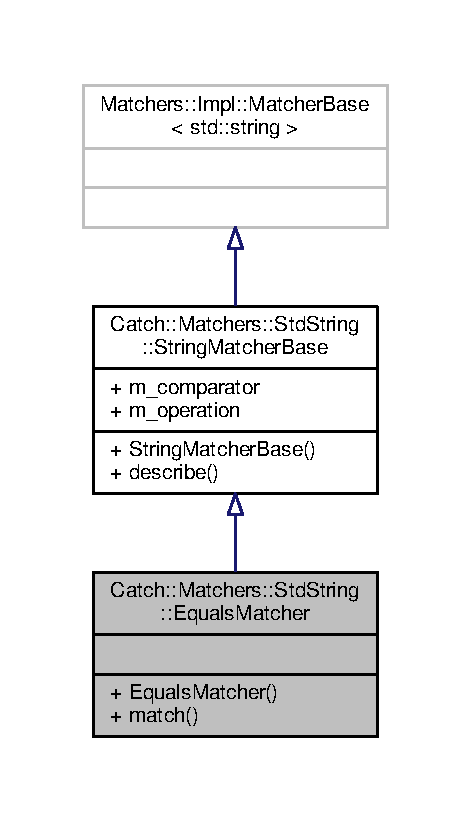
\includegraphics[width=226pt]{struct_catch_1_1_matchers_1_1_std_string_1_1_equals_matcher__inherit__graph}
\end{center}
\end{figure}


Collaboration diagram for Catch\-:\-:Matchers\-:\-:Std\-String\-:\-:Equals\-Matcher\-:
\nopagebreak
\begin{figure}[H]
\begin{center}
\leavevmode
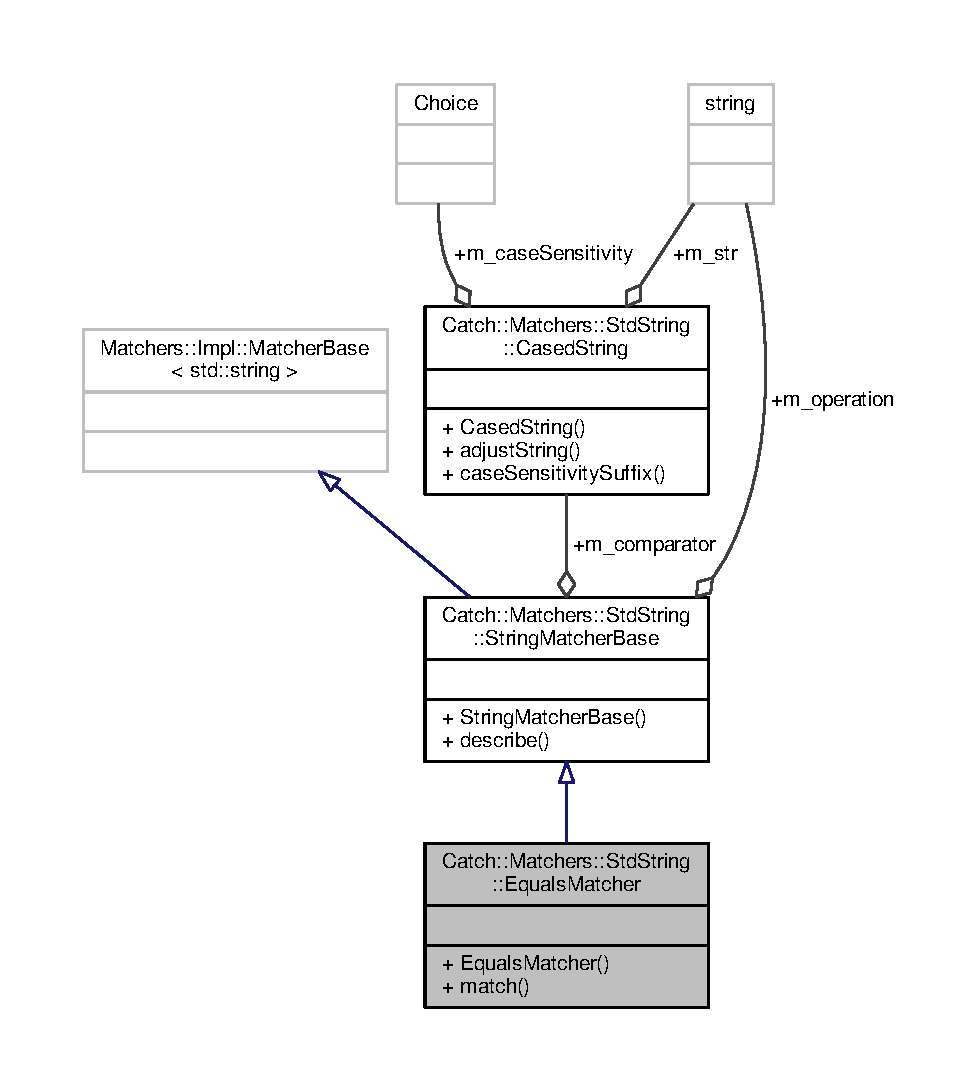
\includegraphics[width=350pt]{struct_catch_1_1_matchers_1_1_std_string_1_1_equals_matcher__coll__graph}
\end{center}
\end{figure}
\subsection*{Public Member Functions}
\begin{DoxyCompactItemize}
\item 
\hyperlink{struct_catch_1_1_matchers_1_1_std_string_1_1_equals_matcher_ab740f1fb2310e9fe3fed5134d4c7e4c8}{Equals\-Matcher} (\hyperlink{struct_catch_1_1_matchers_1_1_std_string_1_1_cased_string}{Cased\-String} const \&comparator)
\item 
bool \hyperlink{struct_catch_1_1_matchers_1_1_std_string_1_1_equals_matcher_a0bb9d64693f7bb1ef7441062d219f21a}{match} (std\-::string const \&source) const override
\end{DoxyCompactItemize}
\subsection*{Additional Inherited Members}


\subsection{Constructor \& Destructor Documentation}
\hypertarget{struct_catch_1_1_matchers_1_1_std_string_1_1_equals_matcher_ab740f1fb2310e9fe3fed5134d4c7e4c8}{\index{Catch\-::\-Matchers\-::\-Std\-String\-::\-Equals\-Matcher@{Catch\-::\-Matchers\-::\-Std\-String\-::\-Equals\-Matcher}!Equals\-Matcher@{Equals\-Matcher}}
\index{Equals\-Matcher@{Equals\-Matcher}!Catch::Matchers::StdString::EqualsMatcher@{Catch\-::\-Matchers\-::\-Std\-String\-::\-Equals\-Matcher}}
\subsubsection[{Equals\-Matcher}]{\setlength{\rightskip}{0pt plus 5cm}Catch\-::\-Matchers\-::\-Std\-String\-::\-Equals\-Matcher\-::\-Equals\-Matcher (
\begin{DoxyParamCaption}
\item[{{\bf Cased\-String} const \&}]{comparator}
\end{DoxyParamCaption}
)}}\label{struct_catch_1_1_matchers_1_1_std_string_1_1_equals_matcher_ab740f1fb2310e9fe3fed5134d4c7e4c8}


\subsection{Member Function Documentation}
\hypertarget{struct_catch_1_1_matchers_1_1_std_string_1_1_equals_matcher_a0bb9d64693f7bb1ef7441062d219f21a}{\index{Catch\-::\-Matchers\-::\-Std\-String\-::\-Equals\-Matcher@{Catch\-::\-Matchers\-::\-Std\-String\-::\-Equals\-Matcher}!match@{match}}
\index{match@{match}!Catch::Matchers::StdString::EqualsMatcher@{Catch\-::\-Matchers\-::\-Std\-String\-::\-Equals\-Matcher}}
\subsubsection[{match}]{\setlength{\rightskip}{0pt plus 5cm}bool Catch\-::\-Matchers\-::\-Std\-String\-::\-Equals\-Matcher\-::match (
\begin{DoxyParamCaption}
\item[{std\-::string const \&}]{source}
\end{DoxyParamCaption}
) const\hspace{0.3cm}{\ttfamily [override]}}}\label{struct_catch_1_1_matchers_1_1_std_string_1_1_equals_matcher_a0bb9d64693f7bb1ef7441062d219f21a}


The documentation for this struct was generated from the following file\-:\begin{DoxyCompactItemize}
\item 
\hyperlink{catch_8hpp}{catch.\-hpp}\end{DoxyCompactItemize}

\hypertarget{struct_catch_1_1_matchers_1_1_vector_1_1_equals_matcher}{\section{Catch\-:\-:Matchers\-:\-:Vector\-:\-:Equals\-Matcher$<$ T $>$ Struct Template Reference}
\label{struct_catch_1_1_matchers_1_1_vector_1_1_equals_matcher}\index{Catch\-::\-Matchers\-::\-Vector\-::\-Equals\-Matcher$<$ T $>$@{Catch\-::\-Matchers\-::\-Vector\-::\-Equals\-Matcher$<$ T $>$}}
}


{\ttfamily \#include $<$catch.\-hpp$>$}



Inheritance diagram for Catch\-:\-:Matchers\-:\-:Vector\-:\-:Equals\-Matcher$<$ T $>$\-:
\nopagebreak
\begin{figure}[H]
\begin{center}
\leavevmode
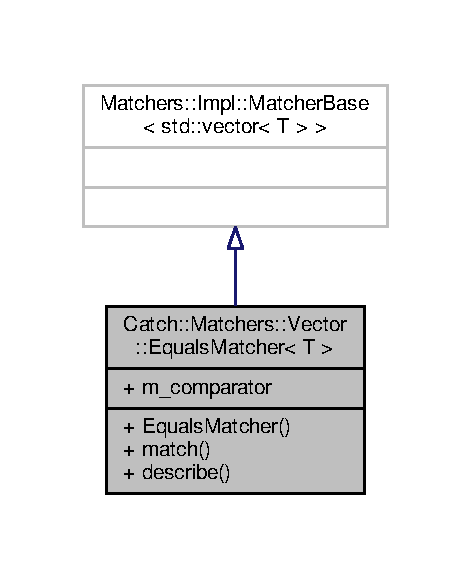
\includegraphics[width=226pt]{struct_catch_1_1_matchers_1_1_vector_1_1_equals_matcher__inherit__graph}
\end{center}
\end{figure}


Collaboration diagram for Catch\-:\-:Matchers\-:\-:Vector\-:\-:Equals\-Matcher$<$ T $>$\-:
\nopagebreak
\begin{figure}[H]
\begin{center}
\leavevmode
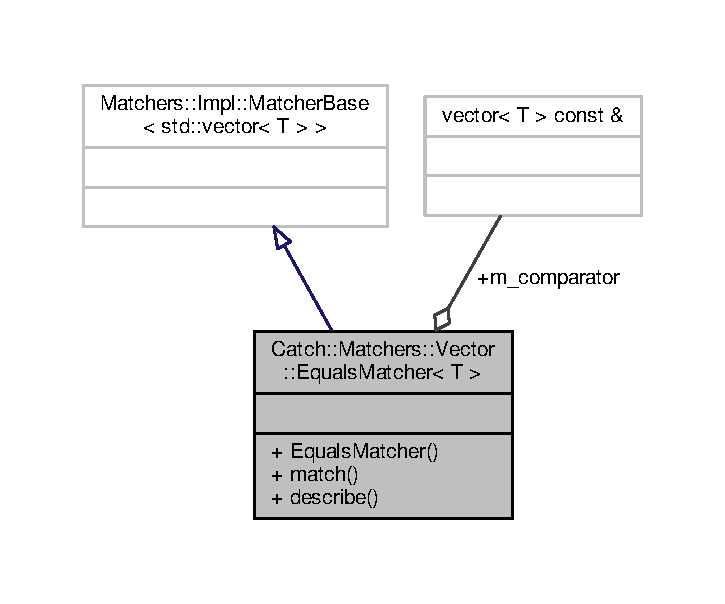
\includegraphics[width=348pt]{struct_catch_1_1_matchers_1_1_vector_1_1_equals_matcher__coll__graph}
\end{center}
\end{figure}
\subsection*{Public Member Functions}
\begin{DoxyCompactItemize}
\item 
\hyperlink{struct_catch_1_1_matchers_1_1_vector_1_1_equals_matcher_a3846c47780d1991dcfe87aefded98008}{Equals\-Matcher} (std\-::vector$<$ T $>$ const \&comparator)
\item 
bool \hyperlink{struct_catch_1_1_matchers_1_1_vector_1_1_equals_matcher_a2d96cca58a44151fddc5257eda3305da}{match} (std\-::vector$<$ T $>$ const \&v) const override
\item 
std\-::string \hyperlink{struct_catch_1_1_matchers_1_1_vector_1_1_equals_matcher_a36b5f7ecada4081d6c65bebe8ddea6f4}{describe} () const override
\end{DoxyCompactItemize}
\subsection*{Public Attributes}
\begin{DoxyCompactItemize}
\item 
std\-::vector$<$ T $>$ const \& \hyperlink{struct_catch_1_1_matchers_1_1_vector_1_1_equals_matcher_a56f7aa6f110a12b1b9aeb0cabbc9d755}{m\-\_\-comparator}
\end{DoxyCompactItemize}


\subsection{Constructor \& Destructor Documentation}
\hypertarget{struct_catch_1_1_matchers_1_1_vector_1_1_equals_matcher_a3846c47780d1991dcfe87aefded98008}{\index{Catch\-::\-Matchers\-::\-Vector\-::\-Equals\-Matcher@{Catch\-::\-Matchers\-::\-Vector\-::\-Equals\-Matcher}!Equals\-Matcher@{Equals\-Matcher}}
\index{Equals\-Matcher@{Equals\-Matcher}!Catch::Matchers::Vector::EqualsMatcher@{Catch\-::\-Matchers\-::\-Vector\-::\-Equals\-Matcher}}
\subsubsection[{Equals\-Matcher}]{\setlength{\rightskip}{0pt plus 5cm}template$<$typename T $>$ {\bf Catch\-::\-Matchers\-::\-Vector\-::\-Equals\-Matcher}$<$ T $>$\-::{\bf Equals\-Matcher} (
\begin{DoxyParamCaption}
\item[{std\-::vector$<$ T $>$ const \&}]{comparator}
\end{DoxyParamCaption}
)\hspace{0.3cm}{\ttfamily [inline]}}}\label{struct_catch_1_1_matchers_1_1_vector_1_1_equals_matcher_a3846c47780d1991dcfe87aefded98008}

\begin{DoxyCode}
2607 : \hyperlink{struct_catch_1_1_matchers_1_1_vector_1_1_equals_matcher_a56f7aa6f110a12b1b9aeb0cabbc9d755}{m\_comparator}(comparator) \{\}
\end{DoxyCode}


\subsection{Member Function Documentation}
\hypertarget{struct_catch_1_1_matchers_1_1_vector_1_1_equals_matcher_a36b5f7ecada4081d6c65bebe8ddea6f4}{\index{Catch\-::\-Matchers\-::\-Vector\-::\-Equals\-Matcher@{Catch\-::\-Matchers\-::\-Vector\-::\-Equals\-Matcher}!describe@{describe}}
\index{describe@{describe}!Catch::Matchers::Vector::EqualsMatcher@{Catch\-::\-Matchers\-::\-Vector\-::\-Equals\-Matcher}}
\subsubsection[{describe}]{\setlength{\rightskip}{0pt plus 5cm}template$<$typename T $>$ std\-::string {\bf Catch\-::\-Matchers\-::\-Vector\-::\-Equals\-Matcher}$<$ T $>$\-::describe (
\begin{DoxyParamCaption}
{}
\end{DoxyParamCaption}
) const\hspace{0.3cm}{\ttfamily [inline]}, {\ttfamily [override]}}}\label{struct_catch_1_1_matchers_1_1_vector_1_1_equals_matcher_a36b5f7ecada4081d6c65bebe8ddea6f4}


References Catch\-::\-Detail\-::stringify().


\begin{DoxyCode}
2621                                                     \{
2622                     \textcolor{keywordflow}{return} \textcolor{stringliteral}{"Equals: "} + \hyperlink{namespace_catch_1_1_detail_af0ad48344ffd3f92f3568465248a9880}{::Catch::Detail::stringify}(
      \hyperlink{struct_catch_1_1_matchers_1_1_vector_1_1_equals_matcher_a56f7aa6f110a12b1b9aeb0cabbc9d755}{m\_comparator});
2623                 \}
\end{DoxyCode}
\hypertarget{struct_catch_1_1_matchers_1_1_vector_1_1_equals_matcher_a2d96cca58a44151fddc5257eda3305da}{\index{Catch\-::\-Matchers\-::\-Vector\-::\-Equals\-Matcher@{Catch\-::\-Matchers\-::\-Vector\-::\-Equals\-Matcher}!match@{match}}
\index{match@{match}!Catch::Matchers::Vector::EqualsMatcher@{Catch\-::\-Matchers\-::\-Vector\-::\-Equals\-Matcher}}
\subsubsection[{match}]{\setlength{\rightskip}{0pt plus 5cm}template$<$typename T $>$ bool {\bf Catch\-::\-Matchers\-::\-Vector\-::\-Equals\-Matcher}$<$ T $>$\-::match (
\begin{DoxyParamCaption}
\item[{std\-::vector$<$ T $>$ const \&}]{v}
\end{DoxyParamCaption}
) const\hspace{0.3cm}{\ttfamily [inline]}, {\ttfamily [override]}}}\label{struct_catch_1_1_matchers_1_1_vector_1_1_equals_matcher_a2d96cca58a44151fddc5257eda3305da}

\begin{DoxyCode}
2609                                                                  \{
2610                     \textcolor{comment}{// !TBD: This currently works if all elements can be compared using !=}
2611                     \textcolor{comment}{// - a more general approach would be via a compare template that defaults}
2612                     \textcolor{comment}{// to using !=. but could be specialised for, e.g. std::vector<T> etc}
2613                     \textcolor{comment}{// - then just call that directly}
2614                     \textcolor{keywordflow}{if} (\hyperlink{struct_catch_1_1_matchers_1_1_vector_1_1_equals_matcher_a56f7aa6f110a12b1b9aeb0cabbc9d755}{m\_comparator}.size() != v.size())
2615                         \textcolor{keywordflow}{return} \textcolor{keyword}{false};
2616                     \textcolor{keywordflow}{for} (std::size\_t i = 0; i < v.size(); ++i)
2617                         \textcolor{keywordflow}{if} (\hyperlink{struct_catch_1_1_matchers_1_1_vector_1_1_equals_matcher_a56f7aa6f110a12b1b9aeb0cabbc9d755}{m\_comparator}[i] != v[i])
2618                             \textcolor{keywordflow}{return} \textcolor{keyword}{false};
2619                     \textcolor{keywordflow}{return} \textcolor{keyword}{true};
2620                 \}
\end{DoxyCode}


\subsection{Member Data Documentation}
\hypertarget{struct_catch_1_1_matchers_1_1_vector_1_1_equals_matcher_a56f7aa6f110a12b1b9aeb0cabbc9d755}{\index{Catch\-::\-Matchers\-::\-Vector\-::\-Equals\-Matcher@{Catch\-::\-Matchers\-::\-Vector\-::\-Equals\-Matcher}!m\-\_\-comparator@{m\-\_\-comparator}}
\index{m\-\_\-comparator@{m\-\_\-comparator}!Catch::Matchers::Vector::EqualsMatcher@{Catch\-::\-Matchers\-::\-Vector\-::\-Equals\-Matcher}}
\subsubsection[{m\-\_\-comparator}]{\setlength{\rightskip}{0pt plus 5cm}template$<$typename T $>$ std\-::vector$<$T$>$ const\& {\bf Catch\-::\-Matchers\-::\-Vector\-::\-Equals\-Matcher}$<$ T $>$\-::m\-\_\-comparator}}\label{struct_catch_1_1_matchers_1_1_vector_1_1_equals_matcher_a56f7aa6f110a12b1b9aeb0cabbc9d755}


The documentation for this struct was generated from the following file\-:\begin{DoxyCompactItemize}
\item 
\hyperlink{catch_8hpp}{catch.\-hpp}\end{DoxyCompactItemize}

\hypertarget{class_catch_1_1_exception_translator_registrar_1_1_exception_translator}{\section{Catch\-:\-:Exception\-Translator\-Registrar\-:\-:Exception\-Translator$<$ T $>$ Class Template Reference}
\label{class_catch_1_1_exception_translator_registrar_1_1_exception_translator}\index{Catch\-::\-Exception\-Translator\-Registrar\-::\-Exception\-Translator$<$ T $>$@{Catch\-::\-Exception\-Translator\-Registrar\-::\-Exception\-Translator$<$ T $>$}}
}


Inheritance diagram for Catch\-:\-:Exception\-Translator\-Registrar\-:\-:Exception\-Translator$<$ T $>$\-:
\nopagebreak
\begin{figure}[H]
\begin{center}
\leavevmode
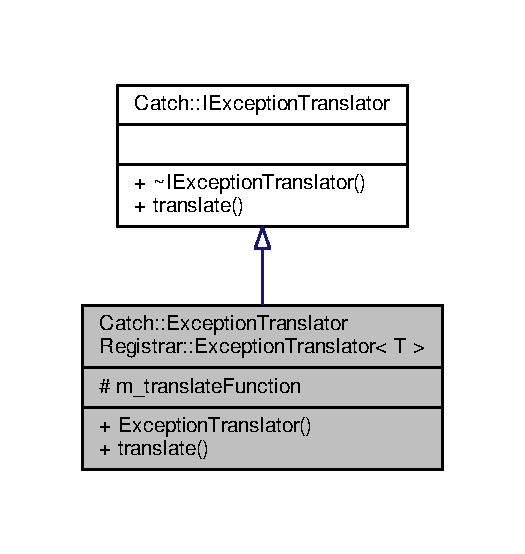
\includegraphics[width=252pt]{class_catch_1_1_exception_translator_registrar_1_1_exception_translator__inherit__graph}
\end{center}
\end{figure}


Collaboration diagram for Catch\-:\-:Exception\-Translator\-Registrar\-:\-:Exception\-Translator$<$ T $>$\-:
\nopagebreak
\begin{figure}[H]
\begin{center}
\leavevmode
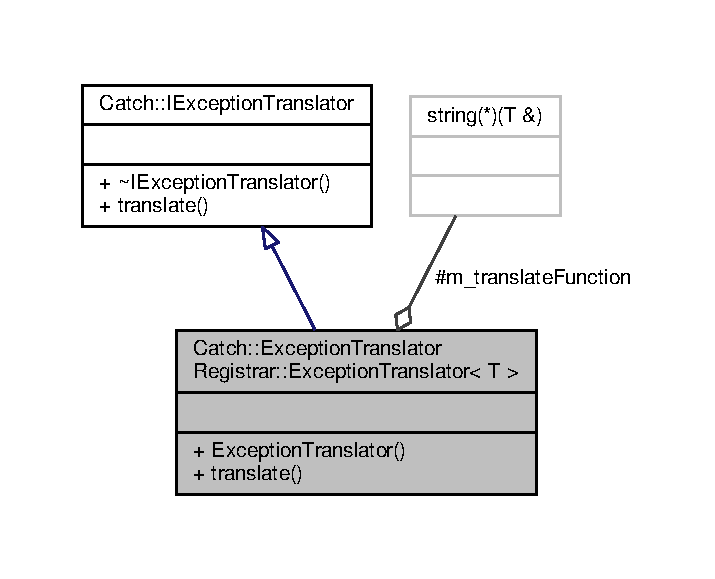
\includegraphics[width=343pt]{class_catch_1_1_exception_translator_registrar_1_1_exception_translator__coll__graph}
\end{center}
\end{figure}
\subsection*{Public Member Functions}
\begin{DoxyCompactItemize}
\item 
\hyperlink{class_catch_1_1_exception_translator_registrar_1_1_exception_translator_a2de4e9bcaad47996159763e69f614d7a}{Exception\-Translator} (std\-::string($\ast$translate\-Function)(T \&))
\item 
std\-::string \hyperlink{class_catch_1_1_exception_translator_registrar_1_1_exception_translator_a29e85940ee9ce719f26e43550cb4ed48}{translate} (Exception\-Translators\-::const\-\_\-iterator it, Exception\-Translators\-::const\-\_\-iterator it\-End) const override
\end{DoxyCompactItemize}
\subsection*{Protected Attributes}
\begin{DoxyCompactItemize}
\item 
std\-::string($\ast$ \hyperlink{class_catch_1_1_exception_translator_registrar_1_1_exception_translator_aa3d9238a0f9b3122a27ac1e60cb79ef9}{m\-\_\-translate\-Function} )(T \&)
\end{DoxyCompactItemize}


\subsection{Constructor \& Destructor Documentation}
\hypertarget{class_catch_1_1_exception_translator_registrar_1_1_exception_translator_a2de4e9bcaad47996159763e69f614d7a}{\index{Catch\-::\-Exception\-Translator\-Registrar\-::\-Exception\-Translator@{Catch\-::\-Exception\-Translator\-Registrar\-::\-Exception\-Translator}!Exception\-Translator@{Exception\-Translator}}
\index{Exception\-Translator@{Exception\-Translator}!Catch::ExceptionTranslatorRegistrar::ExceptionTranslator@{Catch\-::\-Exception\-Translator\-Registrar\-::\-Exception\-Translator}}
\subsubsection[{Exception\-Translator}]{\setlength{\rightskip}{0pt plus 5cm}template$<$typename T $>$ {\bf Catch\-::\-Exception\-Translator\-Registrar\-::\-Exception\-Translator}$<$ T $>$\-::{\bf Exception\-Translator} (
\begin{DoxyParamCaption}
\item[{std\-::string($\ast$)(T \&)}]{translate\-Function}
\end{DoxyParamCaption}
)\hspace{0.3cm}{\ttfamily [inline]}}}\label{class_catch_1_1_exception_translator_registrar_1_1_exception_translator_a2de4e9bcaad47996159763e69f614d7a}

\begin{DoxyCode}
2024                 : \hyperlink{class_catch_1_1_exception_translator_registrar_1_1_exception_translator_aa3d9238a0f9b3122a27ac1e60cb79ef9}{m\_translateFunction}(translateFunction)
2025             \{\}
\end{DoxyCode}


\subsection{Member Function Documentation}
\hypertarget{class_catch_1_1_exception_translator_registrar_1_1_exception_translator_a29e85940ee9ce719f26e43550cb4ed48}{\index{Catch\-::\-Exception\-Translator\-Registrar\-::\-Exception\-Translator@{Catch\-::\-Exception\-Translator\-Registrar\-::\-Exception\-Translator}!translate@{translate}}
\index{translate@{translate}!Catch::ExceptionTranslatorRegistrar::ExceptionTranslator@{Catch\-::\-Exception\-Translator\-Registrar\-::\-Exception\-Translator}}
\subsubsection[{translate}]{\setlength{\rightskip}{0pt plus 5cm}template$<$typename T $>$ std\-::string {\bf Catch\-::\-Exception\-Translator\-Registrar\-::\-Exception\-Translator}$<$ T $>$\-::translate (
\begin{DoxyParamCaption}
\item[{Exception\-Translators\-::const\-\_\-iterator}]{it, }
\item[{Exception\-Translators\-::const\-\_\-iterator}]{it\-End}
\end{DoxyParamCaption}
) const\hspace{0.3cm}{\ttfamily [inline]}, {\ttfamily [override]}, {\ttfamily [virtual]}}}\label{class_catch_1_1_exception_translator_registrar_1_1_exception_translator_a29e85940ee9ce719f26e43550cb4ed48}


Implements \hyperlink{struct_catch_1_1_i_exception_translator_a2a554b96ed5ed411e7c796b6b42837a5}{Catch\-::\-I\-Exception\-Translator}.


\begin{DoxyCode}
2027                                                                                                            
                           \{
2028                 \textcolor{keywordflow}{try} \{
2029                     \textcolor{keywordflow}{if} (it == itEnd)
2030                         std::rethrow\_exception(std::current\_exception());
2031                     \textcolor{keywordflow}{else}
2032                         \textcolor{keywordflow}{return} (*it)->translate(it + 1, itEnd);
2033                 \}
2034                 \textcolor{keywordflow}{catch} (T& ex) \{
2035                     \textcolor{keywordflow}{return} \hyperlink{class_catch_1_1_exception_translator_registrar_1_1_exception_translator_aa3d9238a0f9b3122a27ac1e60cb79ef9}{m\_translateFunction}(ex);
2036                 \}
2037             \}
\end{DoxyCode}


\subsection{Member Data Documentation}
\hypertarget{class_catch_1_1_exception_translator_registrar_1_1_exception_translator_aa3d9238a0f9b3122a27ac1e60cb79ef9}{\index{Catch\-::\-Exception\-Translator\-Registrar\-::\-Exception\-Translator@{Catch\-::\-Exception\-Translator\-Registrar\-::\-Exception\-Translator}!m\-\_\-translate\-Function@{m\-\_\-translate\-Function}}
\index{m\-\_\-translate\-Function@{m\-\_\-translate\-Function}!Catch::ExceptionTranslatorRegistrar::ExceptionTranslator@{Catch\-::\-Exception\-Translator\-Registrar\-::\-Exception\-Translator}}
\subsubsection[{m\-\_\-translate\-Function}]{\setlength{\rightskip}{0pt plus 5cm}template$<$typename T $>$ std\-::string($\ast$ {\bf Catch\-::\-Exception\-Translator\-Registrar\-::\-Exception\-Translator}$<$ T $>$\-::m\-\_\-translate\-Function)(T \&)\hspace{0.3cm}{\ttfamily [protected]}}}\label{class_catch_1_1_exception_translator_registrar_1_1_exception_translator_aa3d9238a0f9b3122a27ac1e60cb79ef9}


The documentation for this class was generated from the following file\-:\begin{DoxyCompactItemize}
\item 
\hyperlink{catch_8hpp}{catch.\-hpp}\end{DoxyCompactItemize}

\hypertarget{class_catch_1_1_exception_translator_registrar}{\section{Catch\-:\-:Exception\-Translator\-Registrar Class Reference}
\label{class_catch_1_1_exception_translator_registrar}\index{Catch\-::\-Exception\-Translator\-Registrar@{Catch\-::\-Exception\-Translator\-Registrar}}
}


{\ttfamily \#include $<$catch.\-hpp$>$}



Collaboration diagram for Catch\-:\-:Exception\-Translator\-Registrar\-:
\nopagebreak
\begin{figure}[H]
\begin{center}
\leavevmode
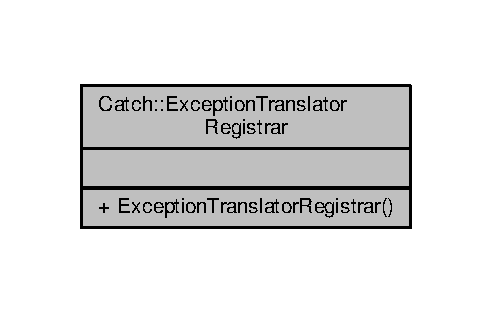
\includegraphics[width=236pt]{class_catch_1_1_exception_translator_registrar__coll__graph}
\end{center}
\end{figure}
\subsection*{Classes}
\begin{DoxyCompactItemize}
\item 
class \hyperlink{class_catch_1_1_exception_translator_registrar_1_1_exception_translator}{Exception\-Translator}
\end{DoxyCompactItemize}
\subsection*{Public Member Functions}
\begin{DoxyCompactItemize}
\item 
{\footnotesize template$<$typename T $>$ }\\\hyperlink{class_catch_1_1_exception_translator_registrar_aa73229de911f26b1df6c6c87c4d9e04e}{Exception\-Translator\-Registrar} (std\-::string($\ast$translate\-Function)(T \&))
\end{DoxyCompactItemize}


\subsection{Constructor \& Destructor Documentation}
\hypertarget{class_catch_1_1_exception_translator_registrar_aa73229de911f26b1df6c6c87c4d9e04e}{\index{Catch\-::\-Exception\-Translator\-Registrar@{Catch\-::\-Exception\-Translator\-Registrar}!Exception\-Translator\-Registrar@{Exception\-Translator\-Registrar}}
\index{Exception\-Translator\-Registrar@{Exception\-Translator\-Registrar}!Catch::ExceptionTranslatorRegistrar@{Catch\-::\-Exception\-Translator\-Registrar}}
\subsubsection[{Exception\-Translator\-Registrar}]{\setlength{\rightskip}{0pt plus 5cm}template$<$typename T $>$ Catch\-::\-Exception\-Translator\-Registrar\-::\-Exception\-Translator\-Registrar (
\begin{DoxyParamCaption}
\item[{std\-::string($\ast$)(T \&)}]{translate\-Function}
\end{DoxyParamCaption}
)\hspace{0.3cm}{\ttfamily [inline]}}}\label{class_catch_1_1_exception_translator_registrar_aa73229de911f26b1df6c6c87c4d9e04e}


References Catch\-::get\-Mutable\-Registry\-Hub(), and Catch\-::\-I\-Mutable\-Registry\-Hub\-::register\-Translator().


\begin{DoxyCode}
2045                                                                         \{
2046             \hyperlink{namespace_catch_ac9ddcc6d66079add9cb2a3140b8ae51e}{getMutableRegistryHub}().\hyperlink{struct_catch_1_1_i_mutable_registry_hub_ae6825365102693cf7707db022a2c2b49}{registerTranslator}
2047             (\textcolor{keyword}{new} ExceptionTranslator<T>(translateFunction));
2048         \}
\end{DoxyCode}


The documentation for this class was generated from the following file\-:\begin{DoxyCompactItemize}
\item 
\hyperlink{catch_8hpp}{catch.\-hpp}\end{DoxyCompactItemize}

\hypertarget{class_catch_1_1_expr_lhs}{\section{Catch\-:\-:Expr\-Lhs$<$ Lhs\-T $>$ Class Template Reference}
\label{class_catch_1_1_expr_lhs}\index{Catch\-::\-Expr\-Lhs$<$ Lhs\-T $>$@{Catch\-::\-Expr\-Lhs$<$ Lhs\-T $>$}}
}


{\ttfamily \#include $<$catch.\-hpp$>$}



Collaboration diagram for Catch\-:\-:Expr\-Lhs$<$ Lhs\-T $>$\-:
\nopagebreak
\begin{figure}[H]
\begin{center}
\leavevmode
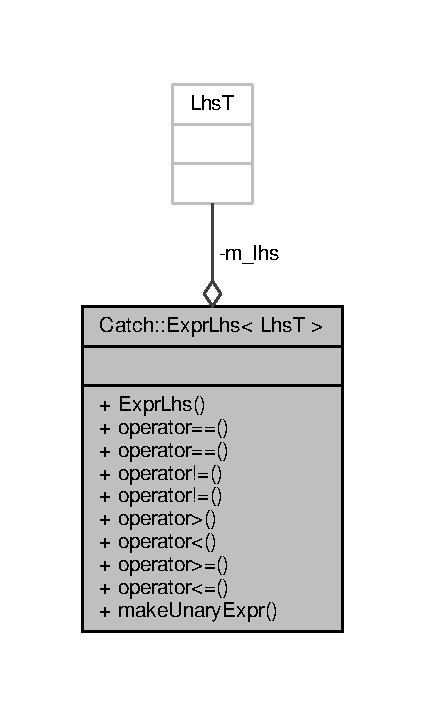
\includegraphics[width=204pt]{class_catch_1_1_expr_lhs__coll__graph}
\end{center}
\end{figure}
\subsection*{Public Member Functions}
\begin{DoxyCompactItemize}
\item 
\hyperlink{class_catch_1_1_expr_lhs_ad22c6af1a7d6993240624d299714a479}{Expr\-Lhs} (Lhs\-T lhs)
\item 
{\footnotesize template$<$typename Rhs\-T $>$ }\\auto \hyperlink{class_catch_1_1_expr_lhs_a96537b7d47cf4567fff40d96637f9b96}{operator==} (Rhs\-T const \&rhs) -\/$>$ \hyperlink{class_catch_1_1_binary_expr}{Binary\-Expr}$<$ Lhs\-T, Rhs\-T const \& $>$ const 
\item 
auto \hyperlink{class_catch_1_1_expr_lhs_ac400741dd25a7b2f00996c7bc48b2075}{operator==} (bool rhs) -\/$>$ \hyperlink{class_catch_1_1_binary_expr}{Binary\-Expr}$<$ Lhs\-T, bool $>$ const 
\item 
{\footnotesize template$<$typename Rhs\-T $>$ }\\auto \hyperlink{class_catch_1_1_expr_lhs_a3ad517cc72c85ae7d06e7a081a3c6cb8}{operator!=} (Rhs\-T const \&rhs) -\/$>$ \hyperlink{class_catch_1_1_binary_expr}{Binary\-Expr}$<$ Lhs\-T, Rhs\-T const \& $>$ const 
\item 
auto \hyperlink{class_catch_1_1_expr_lhs_af45381c45e92bc8182e8790d8b1396b9}{operator!=} (bool rhs) -\/$>$ \hyperlink{class_catch_1_1_binary_expr}{Binary\-Expr}$<$ Lhs\-T, bool $>$ const 
\item 
{\footnotesize template$<$typename Rhs\-T $>$ }\\auto \hyperlink{class_catch_1_1_expr_lhs_aff0149e0c0376f9b2e6763f7fefc5c60}{operator$>$} (Rhs\-T const \&rhs) -\/$>$ \hyperlink{class_catch_1_1_binary_expr}{Binary\-Expr}$<$ Lhs\-T, Rhs\-T const \& $>$ const 
\item 
{\footnotesize template$<$typename Rhs\-T $>$ }\\auto \hyperlink{class_catch_1_1_expr_lhs_a1ae37b86c3156b5fbcaaf02726489f85}{operator$<$} (Rhs\-T const \&rhs) -\/$>$ \hyperlink{class_catch_1_1_binary_expr}{Binary\-Expr}$<$ Lhs\-T, Rhs\-T const \& $>$ const 
\item 
{\footnotesize template$<$typename Rhs\-T $>$ }\\auto \hyperlink{class_catch_1_1_expr_lhs_af367c2fe8f97d6f103988627843ad613}{operator$>$=} (Rhs\-T const \&rhs) -\/$>$ \hyperlink{class_catch_1_1_binary_expr}{Binary\-Expr}$<$ Lhs\-T, Rhs\-T const \& $>$ const 
\item 
{\footnotesize template$<$typename Rhs\-T $>$ }\\auto \hyperlink{class_catch_1_1_expr_lhs_a9a5551293bfe9440ef190cb2b20bc0f8}{operator$<$=} (Rhs\-T const \&rhs) -\/$>$ \hyperlink{class_catch_1_1_binary_expr}{Binary\-Expr}$<$ Lhs\-T, Rhs\-T const \& $>$ const 
\item 
auto \hyperlink{class_catch_1_1_expr_lhs_ab68bd6d5d3ae21b7fba9010150fba95d}{make\-Unary\-Expr} () const -\/$>$ \hyperlink{class_catch_1_1_unary_expr}{Unary\-Expr}$<$ Lhs\-T $>$
\end{DoxyCompactItemize}
\subsection*{Private Attributes}
\begin{DoxyCompactItemize}
\item 
Lhs\-T \hyperlink{class_catch_1_1_expr_lhs_af290873a8427ccbdae6acb915fb7366a}{m\-\_\-lhs}
\end{DoxyCompactItemize}


\subsection{Constructor \& Destructor Documentation}
\hypertarget{class_catch_1_1_expr_lhs_ad22c6af1a7d6993240624d299714a479}{\index{Catch\-::\-Expr\-Lhs@{Catch\-::\-Expr\-Lhs}!Expr\-Lhs@{Expr\-Lhs}}
\index{Expr\-Lhs@{Expr\-Lhs}!Catch::ExprLhs@{Catch\-::\-Expr\-Lhs}}
\subsubsection[{Expr\-Lhs}]{\setlength{\rightskip}{0pt plus 5cm}template$<$typename Lhs\-T$>$ {\bf Catch\-::\-Expr\-Lhs}$<$ Lhs\-T $>$\-::{\bf Expr\-Lhs} (
\begin{DoxyParamCaption}
\item[{Lhs\-T}]{lhs}
\end{DoxyParamCaption}
)\hspace{0.3cm}{\ttfamily [inline]}, {\ttfamily [explicit]}}}\label{class_catch_1_1_expr_lhs_ad22c6af1a7d6993240624d299714a479}

\begin{DoxyCode}
1384 : \hyperlink{class_catch_1_1_expr_lhs_af290873a8427ccbdae6acb915fb7366a}{m\_lhs}(lhs) \{\}
\end{DoxyCode}


\subsection{Member Function Documentation}
\hypertarget{class_catch_1_1_expr_lhs_ab68bd6d5d3ae21b7fba9010150fba95d}{\index{Catch\-::\-Expr\-Lhs@{Catch\-::\-Expr\-Lhs}!make\-Unary\-Expr@{make\-Unary\-Expr}}
\index{make\-Unary\-Expr@{make\-Unary\-Expr}!Catch::ExprLhs@{Catch\-::\-Expr\-Lhs}}
\subsubsection[{make\-Unary\-Expr}]{\setlength{\rightskip}{0pt plus 5cm}template$<$typename Lhs\-T$>$ auto {\bf Catch\-::\-Expr\-Lhs}$<$ Lhs\-T $>$\-::make\-Unary\-Expr (
\begin{DoxyParamCaption}
{}
\end{DoxyParamCaption}
) const -\/$>$ {\bf Unary\-Expr}$<$Lhs\-T$>$ \hspace{0.3cm}{\ttfamily [inline]}}}\label{class_catch_1_1_expr_lhs_ab68bd6d5d3ae21b7fba9010150fba95d}


Referenced by Catch\-::\-Assertion\-Handler\-::handle\-Expr(), and Catch\-::handle\-Expression().


\begin{DoxyCode}
1419                                                       \{
1420             \textcolor{keywordflow}{return} UnaryExpr<LhsT>\{ \hyperlink{class_catch_1_1_expr_lhs_af290873a8427ccbdae6acb915fb7366a}{m\_lhs} \};
1421         \}
\end{DoxyCode}
\hypertarget{class_catch_1_1_expr_lhs_a3ad517cc72c85ae7d06e7a081a3c6cb8}{\index{Catch\-::\-Expr\-Lhs@{Catch\-::\-Expr\-Lhs}!operator!=@{operator!=}}
\index{operator!=@{operator!=}!Catch::ExprLhs@{Catch\-::\-Expr\-Lhs}}
\subsubsection[{operator!=}]{\setlength{\rightskip}{0pt plus 5cm}template$<$typename Lhs\-T$>$ template$<$typename Rhs\-T $>$ auto {\bf Catch\-::\-Expr\-Lhs}$<$ Lhs\-T $>$\-::operator!= (
\begin{DoxyParamCaption}
\item[{Rhs\-T const \&}]{rhs}
\end{DoxyParamCaption}
) -\/$>$ {\bf Binary\-Expr}$<$Lhs\-T, Rhs\-T const\&$>$ const \hspace{0.3cm}{\ttfamily [inline]}}}\label{class_catch_1_1_expr_lhs_a3ad517cc72c85ae7d06e7a081a3c6cb8}


References Catch\-::compare\-Not\-Equal().


\begin{DoxyCode}
1395                                                                                   \{
1396             \textcolor{keywordflow}{return} \{ \hyperlink{namespace_catch_a8bec217f5ef5f09c17074c311c958f3c}{compareNotEqual}(\hyperlink{class_catch_1_1_expr_lhs_af290873a8427ccbdae6acb915fb7366a}{m\_lhs}, rhs), \hyperlink{class_catch_1_1_expr_lhs_af290873a8427ccbdae6acb915fb7366a}{m\_lhs}, \textcolor{stringliteral}{"!="}, rhs \};
1397         \}
\end{DoxyCode}
\hypertarget{class_catch_1_1_expr_lhs_af45381c45e92bc8182e8790d8b1396b9}{\index{Catch\-::\-Expr\-Lhs@{Catch\-::\-Expr\-Lhs}!operator!=@{operator!=}}
\index{operator!=@{operator!=}!Catch::ExprLhs@{Catch\-::\-Expr\-Lhs}}
\subsubsection[{operator!=}]{\setlength{\rightskip}{0pt plus 5cm}template$<$typename Lhs\-T$>$ auto {\bf Catch\-::\-Expr\-Lhs}$<$ Lhs\-T $>$\-::operator!= (
\begin{DoxyParamCaption}
\item[{bool}]{rhs}
\end{DoxyParamCaption}
) -\/$>$ {\bf Binary\-Expr}$<$Lhs\-T, bool$>$ const \hspace{0.3cm}{\ttfamily [inline]}}}\label{class_catch_1_1_expr_lhs_af45381c45e92bc8182e8790d8b1396b9}

\begin{DoxyCode}
1398                                                                     \{
1399             \textcolor{keywordflow}{return} \{ \hyperlink{class_catch_1_1_expr_lhs_af290873a8427ccbdae6acb915fb7366a}{m\_lhs} != rhs, \hyperlink{class_catch_1_1_expr_lhs_af290873a8427ccbdae6acb915fb7366a}{m\_lhs}, \textcolor{stringliteral}{"!="}, rhs \};
1400         \}
\end{DoxyCode}
\hypertarget{class_catch_1_1_expr_lhs_a1ae37b86c3156b5fbcaaf02726489f85}{\index{Catch\-::\-Expr\-Lhs@{Catch\-::\-Expr\-Lhs}!operator$<$@{operator$<$}}
\index{operator$<$@{operator$<$}!Catch::ExprLhs@{Catch\-::\-Expr\-Lhs}}
\subsubsection[{operator$<$}]{\setlength{\rightskip}{0pt plus 5cm}template$<$typename Lhs\-T$>$ template$<$typename Rhs\-T $>$ auto {\bf Catch\-::\-Expr\-Lhs}$<$ Lhs\-T $>$\-::operator$<$ (
\begin{DoxyParamCaption}
\item[{Rhs\-T const \&}]{rhs}
\end{DoxyParamCaption}
) -\/$>$ {\bf Binary\-Expr}$<$Lhs\-T, Rhs\-T const\&$>$ const \hspace{0.3cm}{\ttfamily [inline]}}}\label{class_catch_1_1_expr_lhs_a1ae37b86c3156b5fbcaaf02726489f85}

\begin{DoxyCode}
1407                                                                                  \{
1408             \textcolor{keywordflow}{return} \{ \textcolor{keyword}{static\_cast<}\textcolor{keywordtype}{bool}\textcolor{keyword}{>}(\hyperlink{class_catch_1_1_expr_lhs_af290873a8427ccbdae6acb915fb7366a}{m\_lhs} < rhs), \hyperlink{class_catch_1_1_expr_lhs_af290873a8427ccbdae6acb915fb7366a}{m\_lhs}, \textcolor{stringliteral}{"<"}, rhs \};
1409         \}
\end{DoxyCode}
\hypertarget{class_catch_1_1_expr_lhs_a9a5551293bfe9440ef190cb2b20bc0f8}{\index{Catch\-::\-Expr\-Lhs@{Catch\-::\-Expr\-Lhs}!operator$<$=@{operator$<$=}}
\index{operator$<$=@{operator$<$=}!Catch::ExprLhs@{Catch\-::\-Expr\-Lhs}}
\subsubsection[{operator$<$=}]{\setlength{\rightskip}{0pt plus 5cm}template$<$typename Lhs\-T$>$ template$<$typename Rhs\-T $>$ auto {\bf Catch\-::\-Expr\-Lhs}$<$ Lhs\-T $>$\-::operator$<$= (
\begin{DoxyParamCaption}
\item[{Rhs\-T const \&}]{rhs}
\end{DoxyParamCaption}
) -\/$>$ {\bf Binary\-Expr}$<$Lhs\-T, Rhs\-T const\&$>$ const \hspace{0.3cm}{\ttfamily [inline]}}}\label{class_catch_1_1_expr_lhs_a9a5551293bfe9440ef190cb2b20bc0f8}

\begin{DoxyCode}
1415                                                                                   \{
1416             \textcolor{keywordflow}{return} \{ \textcolor{keyword}{static\_cast<}\textcolor{keywordtype}{bool}\textcolor{keyword}{>}(\hyperlink{class_catch_1_1_expr_lhs_af290873a8427ccbdae6acb915fb7366a}{m\_lhs} <= rhs), \hyperlink{class_catch_1_1_expr_lhs_af290873a8427ccbdae6acb915fb7366a}{m\_lhs}, \textcolor{stringliteral}{"<="}, rhs \};
1417         \}
\end{DoxyCode}
\hypertarget{class_catch_1_1_expr_lhs_a96537b7d47cf4567fff40d96637f9b96}{\index{Catch\-::\-Expr\-Lhs@{Catch\-::\-Expr\-Lhs}!operator==@{operator==}}
\index{operator==@{operator==}!Catch::ExprLhs@{Catch\-::\-Expr\-Lhs}}
\subsubsection[{operator==}]{\setlength{\rightskip}{0pt plus 5cm}template$<$typename Lhs\-T$>$ template$<$typename Rhs\-T $>$ auto {\bf Catch\-::\-Expr\-Lhs}$<$ Lhs\-T $>$\-::operator== (
\begin{DoxyParamCaption}
\item[{Rhs\-T const \&}]{rhs}
\end{DoxyParamCaption}
) -\/$>$ {\bf Binary\-Expr}$<$Lhs\-T, Rhs\-T const\&$>$ const \hspace{0.3cm}{\ttfamily [inline]}}}\label{class_catch_1_1_expr_lhs_a96537b7d47cf4567fff40d96637f9b96}


References Catch\-::compare\-Equal().


\begin{DoxyCode}
1387                                                                                   \{
1388             \textcolor{keywordflow}{return} \{ \hyperlink{namespace_catch_af89b8df30cfaf09abd048c6ff67359ee}{compareEqual}(\hyperlink{class_catch_1_1_expr_lhs_af290873a8427ccbdae6acb915fb7366a}{m\_lhs}, rhs), \hyperlink{class_catch_1_1_expr_lhs_af290873a8427ccbdae6acb915fb7366a}{m\_lhs}, \textcolor{stringliteral}{"=="}, rhs \};
1389         \}
\end{DoxyCode}
\hypertarget{class_catch_1_1_expr_lhs_ac400741dd25a7b2f00996c7bc48b2075}{\index{Catch\-::\-Expr\-Lhs@{Catch\-::\-Expr\-Lhs}!operator==@{operator==}}
\index{operator==@{operator==}!Catch::ExprLhs@{Catch\-::\-Expr\-Lhs}}
\subsubsection[{operator==}]{\setlength{\rightskip}{0pt plus 5cm}template$<$typename Lhs\-T$>$ auto {\bf Catch\-::\-Expr\-Lhs}$<$ Lhs\-T $>$\-::operator== (
\begin{DoxyParamCaption}
\item[{bool}]{rhs}
\end{DoxyParamCaption}
) -\/$>$ {\bf Binary\-Expr}$<$Lhs\-T, bool$>$ const \hspace{0.3cm}{\ttfamily [inline]}}}\label{class_catch_1_1_expr_lhs_ac400741dd25a7b2f00996c7bc48b2075}

\begin{DoxyCode}
1390                                                                     \{
1391             \textcolor{keywordflow}{return} \{ \hyperlink{class_catch_1_1_expr_lhs_af290873a8427ccbdae6acb915fb7366a}{m\_lhs} == rhs, \hyperlink{class_catch_1_1_expr_lhs_af290873a8427ccbdae6acb915fb7366a}{m\_lhs}, \textcolor{stringliteral}{"=="}, rhs \};
1392         \}
\end{DoxyCode}
\hypertarget{class_catch_1_1_expr_lhs_aff0149e0c0376f9b2e6763f7fefc5c60}{\index{Catch\-::\-Expr\-Lhs@{Catch\-::\-Expr\-Lhs}!operator$>$@{operator$>$}}
\index{operator$>$@{operator$>$}!Catch::ExprLhs@{Catch\-::\-Expr\-Lhs}}
\subsubsection[{operator$>$}]{\setlength{\rightskip}{0pt plus 5cm}template$<$typename Lhs\-T$>$ template$<$typename Rhs\-T $>$ auto {\bf Catch\-::\-Expr\-Lhs}$<$ Lhs\-T $>$\-::operator$>$ (
\begin{DoxyParamCaption}
\item[{Rhs\-T const \&}]{rhs}
\end{DoxyParamCaption}
) -\/$>$ {\bf Binary\-Expr}$<$Lhs\-T, Rhs\-T const\&$>$ const \hspace{0.3cm}{\ttfamily [inline]}}}\label{class_catch_1_1_expr_lhs_aff0149e0c0376f9b2e6763f7fefc5c60}

\begin{DoxyCode}
1403                                                                                  \{
1404             \textcolor{keywordflow}{return} \{ \textcolor{keyword}{static\_cast<}\textcolor{keywordtype}{bool}\textcolor{keyword}{>}(\hyperlink{class_catch_1_1_expr_lhs_af290873a8427ccbdae6acb915fb7366a}{m\_lhs} > rhs), \hyperlink{class_catch_1_1_expr_lhs_af290873a8427ccbdae6acb915fb7366a}{m\_lhs}, \textcolor{stringliteral}{">"}, rhs \};
1405         \}
\end{DoxyCode}
\hypertarget{class_catch_1_1_expr_lhs_af367c2fe8f97d6f103988627843ad613}{\index{Catch\-::\-Expr\-Lhs@{Catch\-::\-Expr\-Lhs}!operator$>$=@{operator$>$=}}
\index{operator$>$=@{operator$>$=}!Catch::ExprLhs@{Catch\-::\-Expr\-Lhs}}
\subsubsection[{operator$>$=}]{\setlength{\rightskip}{0pt plus 5cm}template$<$typename Lhs\-T$>$ template$<$typename Rhs\-T $>$ auto {\bf Catch\-::\-Expr\-Lhs}$<$ Lhs\-T $>$\-::operator$>$= (
\begin{DoxyParamCaption}
\item[{Rhs\-T const \&}]{rhs}
\end{DoxyParamCaption}
) -\/$>$ {\bf Binary\-Expr}$<$Lhs\-T, Rhs\-T const\&$>$ const \hspace{0.3cm}{\ttfamily [inline]}}}\label{class_catch_1_1_expr_lhs_af367c2fe8f97d6f103988627843ad613}

\begin{DoxyCode}
1411                                                                                   \{
1412             \textcolor{keywordflow}{return} \{ \textcolor{keyword}{static\_cast<}\textcolor{keywordtype}{bool}\textcolor{keyword}{>}(\hyperlink{class_catch_1_1_expr_lhs_af290873a8427ccbdae6acb915fb7366a}{m\_lhs} >= rhs), \hyperlink{class_catch_1_1_expr_lhs_af290873a8427ccbdae6acb915fb7366a}{m\_lhs}, \textcolor{stringliteral}{">="}, rhs \};
1413         \}
\end{DoxyCode}


\subsection{Member Data Documentation}
\hypertarget{class_catch_1_1_expr_lhs_af290873a8427ccbdae6acb915fb7366a}{\index{Catch\-::\-Expr\-Lhs@{Catch\-::\-Expr\-Lhs}!m\-\_\-lhs@{m\-\_\-lhs}}
\index{m\-\_\-lhs@{m\-\_\-lhs}!Catch::ExprLhs@{Catch\-::\-Expr\-Lhs}}
\subsubsection[{m\-\_\-lhs}]{\setlength{\rightskip}{0pt plus 5cm}template$<$typename Lhs\-T$>$ Lhs\-T {\bf Catch\-::\-Expr\-Lhs}$<$ Lhs\-T $>$\-::m\-\_\-lhs\hspace{0.3cm}{\ttfamily [private]}}}\label{class_catch_1_1_expr_lhs_af290873a8427ccbdae6acb915fb7366a}


The documentation for this class was generated from the following file\-:\begin{DoxyCompactItemize}
\item 
\hyperlink{catch_8hpp}{catch.\-hpp}\end{DoxyCompactItemize}

\hypertarget{class_game}{\section{Game Class Reference}
\label{class_game}\index{Game@{Game}}
}


{\ttfamily \#include $<$Game.\-h$>$}



Collaboration diagram for Game\-:
\nopagebreak
\begin{figure}[H]
\begin{center}
\leavevmode
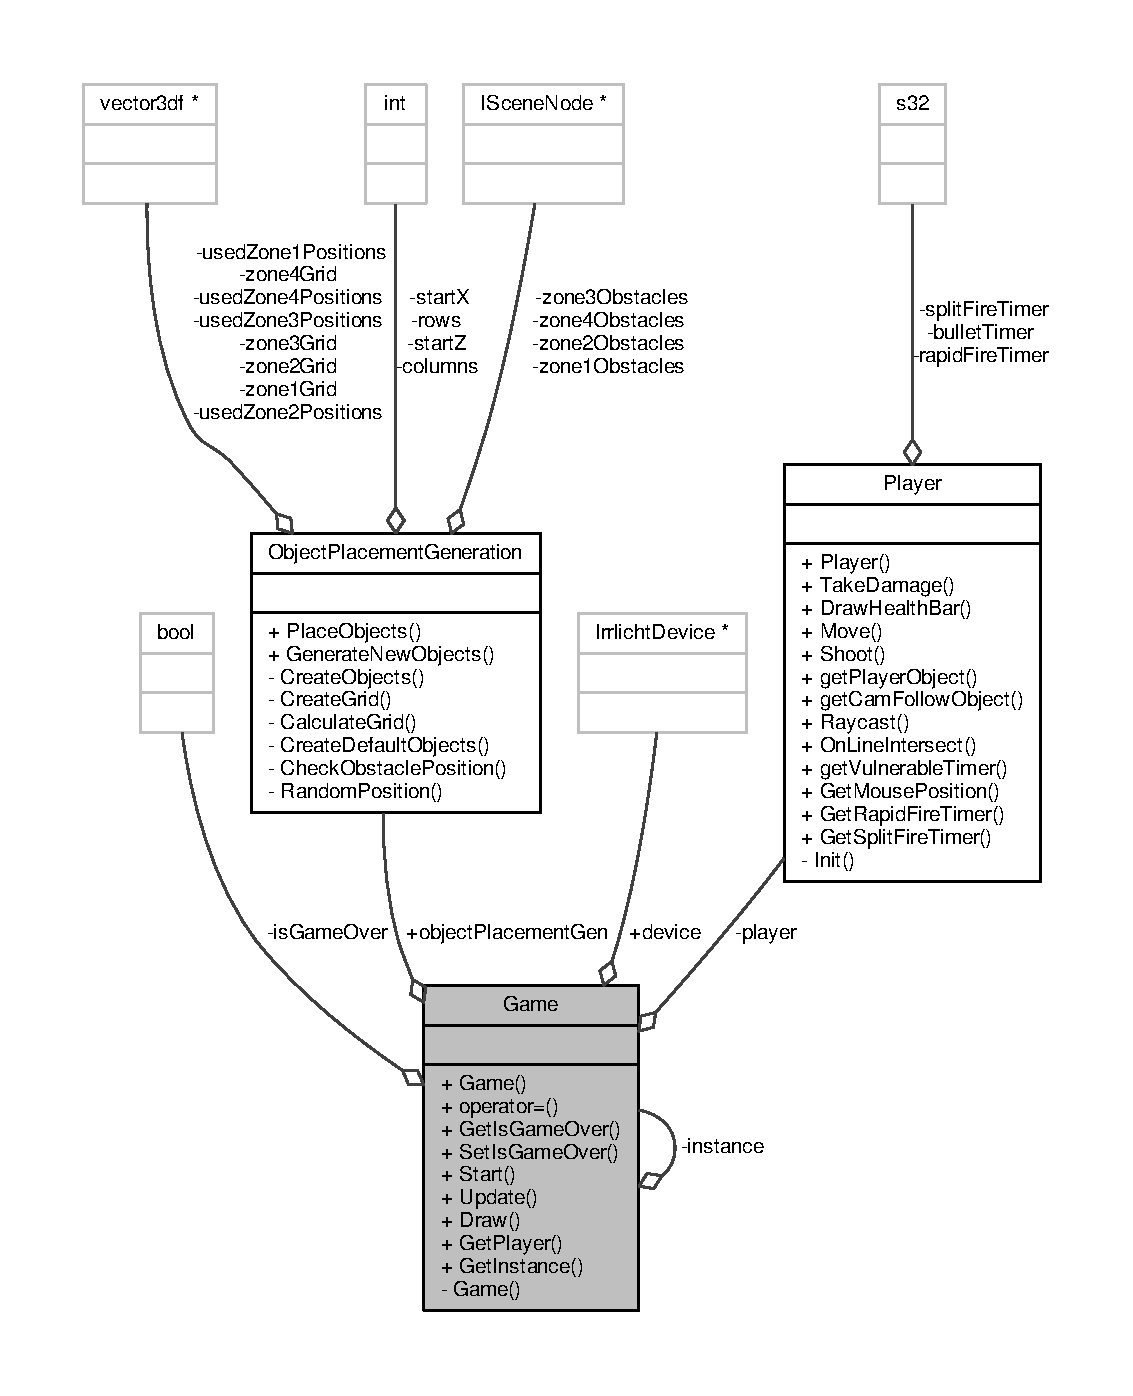
\includegraphics[width=350pt]{class_game__coll__graph}
\end{center}
\end{figure}
\subsection*{Public Member Functions}
\begin{DoxyCompactItemize}
\item 
\hyperlink{class_game_abb28875d74d25fa9e0dcdbe37c6ad89c}{Game} (const \hyperlink{class_game}{Game} \&)=delete
\item 
\hyperlink{class_game}{Game} \& \hyperlink{class_game_a4d0c0503733cc50b0b5cb8d7ef1237ec}{operator=} (const \hyperlink{class_game}{Game} \&)=delete
\item 
bool \hyperlink{class_game_a472e76af50d5275142522f9a5e149ab1}{Get\-Is\-Game\-Over} ()
\item 
bool \hyperlink{class_game_acd4aa68f7ef7603ecd61a879fe0286e7}{Set\-Is\-Game\-Over} (bool state)
\item 
void \hyperlink{class_game_adb05b20574551a26f8cf1dc664782790}{Start} ()
\item 
void \hyperlink{class_game_a1c5373c68261c54aff03e6abe40fee52}{Update} ()
\item 
void \hyperlink{class_game_aad2c20e2c5529244095c50c238911e30}{Draw} ()
\item 
\hyperlink{class_player}{Player} $\ast$ \hyperlink{class_game_ae09ac6fe3bf0d17657cd315e639f8fa4}{Get\-Player} ()
\end{DoxyCompactItemize}
\subsection*{Static Public Member Functions}
\begin{DoxyCompactItemize}
\item 
static \hyperlink{class_game}{Game} $\ast$ \hyperlink{class_game_aa989d3cee96d5ae093663bf62dea57e2}{Get\-Instance} ()
\end{DoxyCompactItemize}
\subsection*{Public Attributes}
\begin{DoxyCompactItemize}
\item 
irr\-::\-Irrlicht\-Device $\ast$ \hyperlink{class_game_a4968552e2ba3037d494596a908eccc00}{device}
\item 
\hyperlink{class_object_placement_generation}{Object\-Placement\-Generation} \hyperlink{class_game_a582b0adfa98534d79ec9511919827029}{object\-Placement\-Gen}
\end{DoxyCompactItemize}
\subsection*{Private Member Functions}
\begin{DoxyCompactItemize}
\item 
\hyperlink{class_game_ad59df6562a58a614fda24622d3715b65}{Game} ()
\end{DoxyCompactItemize}
\subsection*{Private Attributes}
\begin{DoxyCompactItemize}
\item 
bool \hyperlink{class_game_a80544462b0a02a5d30d238cbe7380492}{is\-Game\-Over} = false
\item 
\hyperlink{class_player}{Player} $\ast$ \hyperlink{class_game_abec70aa1c0269a9a7e171af4d79e08bf}{player}
\end{DoxyCompactItemize}
\subsection*{Static Private Attributes}
\begin{DoxyCompactItemize}
\item 
static \hyperlink{class_game}{Game} $\ast$ \hyperlink{class_game_aa469cdc0a30f4fd2d6d99b23f4fbf257}{instance} = 0
\end{DoxyCompactItemize}


\subsection{Constructor \& Destructor Documentation}
\hypertarget{class_game_abb28875d74d25fa9e0dcdbe37c6ad89c}{\index{Game@{Game}!Game@{Game}}
\index{Game@{Game}!Game@{Game}}
\subsubsection[{Game}]{\setlength{\rightskip}{0pt plus 5cm}Game\-::\-Game (
\begin{DoxyParamCaption}
\item[{const {\bf Game} \&}]{}
\end{DoxyParamCaption}
)\hspace{0.3cm}{\ttfamily [delete]}}}\label{class_game_abb28875d74d25fa9e0dcdbe37c6ad89c}
\hypertarget{class_game_ad59df6562a58a614fda24622d3715b65}{\index{Game@{Game}!Game@{Game}}
\index{Game@{Game}!Game@{Game}}
\subsubsection[{Game}]{\setlength{\rightskip}{0pt plus 5cm}Game\-::\-Game (
\begin{DoxyParamCaption}
{}
\end{DoxyParamCaption}
)\hspace{0.3cm}{\ttfamily [private]}}}\label{class_game_ad59df6562a58a614fda24622d3715b65}


References input\-Receiver.


\begin{DoxyCode}
51 \{
52     \textcolor{comment}{// Create device}
53     \hyperlink{class_game_a4968552e2ba3037d494596a908eccc00}{device} = createDevice(EDT\_DIRECT3D9,
54         dimension2d<u32>(800, 600), 16, \textcolor{keyword}{false}, \textcolor{keyword}{false}, \textcolor{keyword}{true}, &\hyperlink{_game_8cpp_ab1a0fe3a591398ca440c6d1932a73be2}{inputReceiver});
55 \}
\end{DoxyCode}


\subsection{Member Function Documentation}
\hypertarget{class_game_aad2c20e2c5529244095c50c238911e30}{\index{Game@{Game}!Draw@{Draw}}
\index{Draw@{Draw}!Game@{Game}}
\subsubsection[{Draw}]{\setlength{\rightskip}{0pt plus 5cm}void Game\-::\-Draw (
\begin{DoxyParamCaption}
{}
\end{DoxyParamCaption}
)}}\label{class_game_aad2c20e2c5529244095c50c238911e30}


References Player\-::\-Draw\-Health\-Bar(), driver, guienv, last\-F\-P\-S, player, score, Score\-::\-Scoring(), smgr, u\-I\-System, and U\-I\-System\-::\-Wave\-U\-I().



Referenced by main().


\begin{DoxyCode}
138 \{
139     \hyperlink{_game_8cpp_ae8ebff0dce398b6764c0e99ec847754a}{driver}->beginScene(\textcolor{keyword}{true}, \textcolor{keyword}{true}, SColor(255, 113, 113, 133));
140     \hyperlink{_game_8cpp_a80a0cf5a63a07fec786bf483e5f22c39}{smgr}->drawAll();
141     \hyperlink{_game_8cpp_ac1b59d355d5bebba653a1a6a4a6a2e19}{guienv}->drawAll();
142     \hyperlink{class_game_abec70aa1c0269a9a7e171af4d79e08bf}{player}->\hyperlink{class_player_aa6cc636d92ca5ccba15a5af2ef7f224a}{DrawHealthBar}();
143     \hyperlink{_game_8cpp_a94014506ee2a0c05dcb878c5f6a1ce0f}{score}.\hyperlink{class_score_ae8d4105bea77e4bfcd77c347e0a9dd8c}{Scoring}(\hyperlink{class_game_a4968552e2ba3037d494596a908eccc00}{device});
144     \hyperlink{_game_8cpp_a968f4669d04899e10a3f52223cd20811}{uISystem}->\hyperlink{class_u_i_system_a41981a6094a5dcb0fcd180660722138a}{WaveUI}(\hyperlink{class_game_a4968552e2ba3037d494596a908eccc00}{device});
145     \hyperlink{_game_8cpp_ae8ebff0dce398b6764c0e99ec847754a}{driver}->endScene();
146 
147     \textcolor{keywordtype}{int} fps = \hyperlink{_game_8cpp_ae8ebff0dce398b6764c0e99ec847754a}{driver}->getFPS();
148     \textcolor{keywordflow}{if} (\hyperlink{_game_8cpp_ad465136e518210a5b41ec8546cf4bd9d}{lastFPS} != fps)
149     \{
150         stringw tmp(L\textcolor{stringliteral}{"KOMMANDOS - Irrlicht Engine"});
151 
152         tmp += \hyperlink{_game_8cpp_ae8ebff0dce398b6764c0e99ec847754a}{driver}->getName();
153         tmp += L\textcolor{stringliteral}{"] fps: "};
154         tmp += fps;
155 
156         \hyperlink{class_game_a4968552e2ba3037d494596a908eccc00}{device}->setWindowCaption(tmp.c\_str());
157         \hyperlink{_game_8cpp_ad465136e518210a5b41ec8546cf4bd9d}{lastFPS} = fps;
158     \}
159 \}
\end{DoxyCode}
\hypertarget{class_game_aa989d3cee96d5ae093663bf62dea57e2}{\index{Game@{Game}!Get\-Instance@{Get\-Instance}}
\index{Get\-Instance@{Get\-Instance}!Game@{Game}}
\subsubsection[{Get\-Instance}]{\setlength{\rightskip}{0pt plus 5cm}{\bf Game} $\ast$ Game\-::\-Get\-Instance (
\begin{DoxyParamCaption}
{}
\end{DoxyParamCaption}
)\hspace{0.3cm}{\ttfamily [static]}}}\label{class_game_aa989d3cee96d5ae093663bf62dea57e2}


Referenced by Camera\-::\-Camera(), Enemy\-Spawner\-::\-Enemy\-Spawner(), Object\-Placement\-Generation\-::\-Generate\-New\-Objects(), U\-I\-System\-::\-Init\-U\-I\-System(), main(), Player\-::\-Player(), Score\-::\-Scoring(), and U\-I\-System\-::\-U\-I\-System().


\begin{DoxyCode}
60                         \{
61     \textcolor{keywordflow}{if} (!\hyperlink{class_game_aa469cdc0a30f4fd2d6d99b23f4fbf257}{instance})
62     \{
63         \hyperlink{class_game_aa469cdc0a30f4fd2d6d99b23f4fbf257}{instance} = \textcolor{keyword}{new} \hyperlink{class_game_ad59df6562a58a614fda24622d3715b65}{Game}();
64     \}
65     \textcolor{keywordflow}{return} \hyperlink{class_game_aa469cdc0a30f4fd2d6d99b23f4fbf257}{instance};
66 \}
\end{DoxyCode}
\hypertarget{class_game_a472e76af50d5275142522f9a5e149ab1}{\index{Game@{Game}!Get\-Is\-Game\-Over@{Get\-Is\-Game\-Over}}
\index{Get\-Is\-Game\-Over@{Get\-Is\-Game\-Over}!Game@{Game}}
\subsubsection[{Get\-Is\-Game\-Over}]{\setlength{\rightskip}{0pt plus 5cm}bool Game\-::\-Get\-Is\-Game\-Over (
\begin{DoxyParamCaption}
{}
\end{DoxyParamCaption}
)}}\label{class_game_a472e76af50d5275142522f9a5e149ab1}


References is\-Game\-Over.



Referenced by Player\-::\-Draw\-Health\-Bar(), Score\-::\-Scoring(), Enemy\-Spawner\-::\-Update\-Enemies(), and U\-I\-System\-::\-Wave\-U\-I().


\begin{DoxyCode}
68                          \{
69     \textcolor{keywordflow}{return} \hyperlink{class_game_a80544462b0a02a5d30d238cbe7380492}{isGameOver};
70 \}
\end{DoxyCode}
\hypertarget{class_game_ae09ac6fe3bf0d17657cd315e639f8fa4}{\index{Game@{Game}!Get\-Player@{Get\-Player}}
\index{Get\-Player@{Get\-Player}!Game@{Game}}
\subsubsection[{Get\-Player}]{\setlength{\rightskip}{0pt plus 5cm}{\bf Player} $\ast$ Game\-::\-Get\-Player (
\begin{DoxyParamCaption}
{}
\end{DoxyParamCaption}
)}}\label{class_game_ae09ac6fe3bf0d17657cd315e639f8fa4}


References player.



Referenced by U\-I\-System\-::\-Init\-U\-I\-System().


\begin{DoxyCode}
162 \{
163     \textcolor{keywordflow}{return} \hyperlink{class_game_abec70aa1c0269a9a7e171af4d79e08bf}{player};
164 \}\end{DoxyCode}
\hypertarget{class_game_a4d0c0503733cc50b0b5cb8d7ef1237ec}{\index{Game@{Game}!operator=@{operator=}}
\index{operator=@{operator=}!Game@{Game}}
\subsubsection[{operator=}]{\setlength{\rightskip}{0pt plus 5cm}{\bf Game}\& Game\-::operator= (
\begin{DoxyParamCaption}
\item[{const {\bf Game} \&}]{}
\end{DoxyParamCaption}
)\hspace{0.3cm}{\ttfamily [delete]}}}\label{class_game_a4d0c0503733cc50b0b5cb8d7ef1237ec}
\hypertarget{class_game_acd4aa68f7ef7603ecd61a879fe0286e7}{\index{Game@{Game}!Set\-Is\-Game\-Over@{Set\-Is\-Game\-Over}}
\index{Set\-Is\-Game\-Over@{Set\-Is\-Game\-Over}!Game@{Game}}
\subsubsection[{Set\-Is\-Game\-Over}]{\setlength{\rightskip}{0pt plus 5cm}bool Game\-::\-Set\-Is\-Game\-Over (
\begin{DoxyParamCaption}
\item[{bool}]{state}
\end{DoxyParamCaption}
)}}\label{class_game_acd4aa68f7ef7603ecd61a879fe0286e7}


References camera, Camera\-::gameover, is\-Game\-Over, Tutorial\-::\-Remove\-Tutorial(), Camera\-::state, and tutorial.



Referenced by Player\-::\-Take\-Damage().


\begin{DoxyCode}
73 \{
74     \hyperlink{_game_8cpp_ae2e07e9072887b6ad4c087d948f1a431}{tutorial}.\hyperlink{class_tutorial_a0bef62d9bb8e461bfa119e80bacc1ca5}{RemoveTutorial}();
75     \hyperlink{_game_8cpp_af95833c961e5bd20dcd54e1d46a03c0b}{camera}->\hyperlink{class_camera_a87960570c2d28bd4471c5a74fc021cb5}{state} = \hyperlink{_game_8cpp_af95833c961e5bd20dcd54e1d46a03c0b}{camera}->\hyperlink{class_camera_a1ddf5d726e6c1d1d1c08d96d42c40236a4d150a6fd04ef129c37e767d9087fa9f}{gameover};
76     \textcolor{keywordflow}{return} \hyperlink{class_game_a80544462b0a02a5d30d238cbe7380492}{isGameOver} = state;
77 \}
\end{DoxyCode}
\hypertarget{class_game_adb05b20574551a26f8cf1dc664782790}{\index{Game@{Game}!Start@{Start}}
\index{Start@{Start}!Game@{Game}}
\subsubsection[{Start}]{\setlength{\rightskip}{0pt plus 5cm}void Game\-::\-Start (
\begin{DoxyParamCaption}
{}
\end{DoxyParamCaption}
)}}\label{class_game_adb05b20574551a26f8cf1dc664782790}


References camera, driver, enemy\-Spawner, Sound\-Manager\-::\-Get\-Instance(), Camera\-::\-Get\-Instance(), guienv, U\-I\-System\-::\-Init\-U\-I\-System(), player, Sound\-Manager\-::\-Play\-Sound(), power\-Spawn, Power\-Up\-Spawner\-::\-Power\-Up\-Device(), prev\-Frame, score, Score\-::\-Scoring(), Tutorial\-::\-Show\-Tutorial(), smgr, sound\-Manager, tutorial, and u\-I\-System.



Referenced by main().


\begin{DoxyCode}
81 \{
82     \textcolor{comment}{//Get the sound engine}
83     \hyperlink{class_sound_manager}{SoundManager}* \hyperlink{_player_8cpp_aa536d458e5b766e20ac204a4ab09cc36}{soundManager} = soundManager->
      \hyperlink{class_sound_manager_a887480b38c9380c9fba23a2337df63be}{GetInstance}();
84     \textcolor{comment}{//Start Game Background song    }
85     soundManager->\hyperlink{class_sound_manager_a81e8f88fe549f6767d3552f12c28ecbc}{PlaySound}(\textcolor{stringliteral}{"../media/Sounds/bgsound.mp3"}, \textcolor{keyword}{true});
86 
87     \textcolor{comment}{// Create instances of classes}
88     \hyperlink{_game_8cpp_af95833c961e5bd20dcd54e1d46a03c0b}{camera} = \hyperlink{_game_8cpp_af95833c961e5bd20dcd54e1d46a03c0b}{camera}->\hyperlink{class_camera_aae2256f0ee62dd982d92c09d9d00c8d5}{GetInstance}(\hyperlink{class_game_a4968552e2ba3037d494596a908eccc00}{device});
89     \hyperlink{class_game_abec70aa1c0269a9a7e171af4d79e08bf}{player} = \textcolor{keyword}{new} \hyperlink{class_player}{Player}(\hyperlink{class_game_a4968552e2ba3037d494596a908eccc00}{device});
90     \hyperlink{_game_8cpp_a78dc0d7de0179cebaebf79df72c6070f}{enemySpawner} = \textcolor{keyword}{new} \hyperlink{class_enemy_spawner}{EnemySpawner}(\hyperlink{class_game_a4968552e2ba3037d494596a908eccc00}{device}, \hyperlink{class_game_abec70aa1c0269a9a7e171af4d79e08bf}{player});
91     \hyperlink{_game_8cpp_a968f4669d04899e10a3f52223cd20811}{uISystem} = \textcolor{keyword}{new} \hyperlink{class_u_i_system}{UISystem}(\hyperlink{class_game_a4968552e2ba3037d494596a908eccc00}{device});
92 
93     \textcolor{comment}{//score.Scoring is unneeded duplicate code}
94     \hyperlink{_game_8cpp_a94014506ee2a0c05dcb878c5f6a1ce0f}{score}.\hyperlink{class_score_ae8d4105bea77e4bfcd77c347e0a9dd8c}{Scoring}(\hyperlink{class_game_a4968552e2ba3037d494596a908eccc00}{device});
95     \hyperlink{_game_8cpp_ae2e07e9072887b6ad4c087d948f1a431}{tutorial}.\hyperlink{class_tutorial_a2bcccb05a09cfb9cd14fb456a609c50b}{ShowTutorial}(\hyperlink{class_game_a4968552e2ba3037d494596a908eccc00}{device});
96 
97     \hyperlink{_game_8cpp_ae8ebff0dce398b6764c0e99ec847754a}{driver} = \hyperlink{class_game_a4968552e2ba3037d494596a908eccc00}{device}->getVideoDriver();
98     \hyperlink{_game_8cpp_a80a0cf5a63a07fec786bf483e5f22c39}{smgr} = \hyperlink{class_game_a4968552e2ba3037d494596a908eccc00}{device}->getSceneManager();
99     \hyperlink{_game_8cpp_ac1b59d355d5bebba653a1a6a4a6a2e19}{guienv} = \hyperlink{class_game_a4968552e2ba3037d494596a908eccc00}{device}->getGUIEnvironment();
100 
101     \hyperlink{class_game_a582b0adfa98534d79ec9511919827029}{objectPlacementGen}.\hyperlink{class_object_placement_generation_a94bc6a7a4ea7001bff3799cd9da12481}{PlaceObjects}(\hyperlink{class_game_a4968552e2ba3037d494596a908eccc00}{device});
102     \hyperlink{_game_8cpp_a8b36d1e84444017dfabce4f05ad6006f}{powerSpawn}->\hyperlink{class_power_up_spawner_ad95f01d926ce8438046b4c8f7aa99d9e}{PowerUpDevice}(\hyperlink{class_game_a4968552e2ba3037d494596a908eccc00}{device});
103 
104     \hyperlink{_game_8cpp_a968f4669d04899e10a3f52223cd20811}{uISystem}->\hyperlink{class_u_i_system_aa614552df8a07d24661719d007ea8baf}{InitUISystem}(\hyperlink{class_game_a4968552e2ba3037d494596a908eccc00}{device});
105 
106     \textcolor{comment}{//Create Light}
107     ILightSceneNode*  directionalLight = \hyperlink{class_game_a4968552e2ba3037d494596a908eccc00}{device}->getSceneManager()->addLightSceneNode();
108     SLight & lightData = directionalLight->getLightData();
109     lightData.Type = ELT\_DIRECTIONAL;
110     directionalLight->setRotation(vector3df(90, 0, 0));
111     \hyperlink{class_game_a4968552e2ba3037d494596a908eccc00}{device}->getCursorControl()->setVisible(\textcolor{keyword}{true});
112 
113     \textcolor{comment}{//This is used to calculate frame delta time}
114     \hyperlink{_game_8cpp_a0ff1af7dce63798c7cd58af0841a0a73}{prevFrame} = \hyperlink{class_game_a4968552e2ba3037d494596a908eccc00}{device}->getTimer()->getTime();
115 \}
\end{DoxyCode}
\hypertarget{class_game_a1c5373c68261c54aff03e6abe40fee52}{\index{Game@{Game}!Update@{Update}}
\index{Update@{Update}!Game@{Game}}
\subsubsection[{Update}]{\setlength{\rightskip}{0pt plus 5cm}void Game\-::\-Update (
\begin{DoxyParamCaption}
{}
\end{DoxyParamCaption}
)}}\label{class_game_a1c5373c68261c54aff03e6abe40fee52}


References camera, Camera\-::\-Camera\-Update(), collision\-Manager, Collision\-::\-Discrete\-Collision\-Update(), enemy\-Spawner, frame\-Delta\-Time, input\-Receiver, is\-Game\-Over, Tutorial\-::is\-Tutorial\-Active, Player\-::\-Move(), player, prev\-Frame, Player\-::\-Shoot(), tutorial, Tutorial\-::\-Update(), and Enemy\-Spawner\-::\-Update\-Enemies().



Referenced by main().


\begin{DoxyCode}
118 \{
119     \textcolor{comment}{// Work out a frame delta time.}
120     \textcolor{keyword}{const} u32 currentFrame = \hyperlink{class_game_a4968552e2ba3037d494596a908eccc00}{device}->getTimer()->getTime();
121     \textcolor{keyword}{const} f32 \hyperlink{_player_8cpp_adc988571147642cda93afbf89783f9c9}{frameDeltaTime} = (f32)(currentFrame - \hyperlink{_game_8cpp_a0ff1af7dce63798c7cd58af0841a0a73}{prevFrame}) / 1000.f; \textcolor{comment}{// Time in
       seconds}
122     \hyperlink{_game_8cpp_a0ff1af7dce63798c7cd58af0841a0a73}{prevFrame} = currentFrame;
123     \hyperlink{_game_8cpp_af95833c961e5bd20dcd54e1d46a03c0b}{camera}->\hyperlink{class_camera_a76e6167aa081ea6755d0bf588cd8cb73}{CameraUpdate}(frameDeltaTime);
124     \textcolor{keywordflow}{if} (\hyperlink{_game_8cpp_ae2e07e9072887b6ad4c087d948f1a431}{tutorial}.\hyperlink{class_tutorial_a050c9844b3a52de799105883893ca073}{isTutorialActive}) \{
125         \hyperlink{_game_8cpp_ae2e07e9072887b6ad4c087d948f1a431}{tutorial}.\hyperlink{class_tutorial_a3c755730bce8d71fdd9137a048e7c732}{Update}(frameDeltaTime);
126     \}
127     \textcolor{keywordflow}{if} (!\hyperlink{class_game_a80544462b0a02a5d30d238cbe7380492}{isGameOver} )
128     \{
129         \hyperlink{class_game_abec70aa1c0269a9a7e171af4d79e08bf}{player}->\hyperlink{class_player_a436296b5c3aca2e448563594fc3eb234}{Move}(\hyperlink{_game_8cpp_ab1a0fe3a591398ca440c6d1932a73be2}{inputReceiver});
130         \hyperlink{class_game_abec70aa1c0269a9a7e171af4d79e08bf}{player}->\hyperlink{class_player_a24b813efa1554eeb30cd7e3b508bf8fd}{Shoot}(\hyperlink{_game_8cpp_ab1a0fe3a591398ca440c6d1932a73be2}{inputReceiver}, \hyperlink{_game_8cpp_a78dc0d7de0179cebaebf79df72c6070f}{enemySpawner});
131         \textcolor{keywordflow}{if}(!\hyperlink{_game_8cpp_ae2e07e9072887b6ad4c087d948f1a431}{tutorial}.\hyperlink{class_tutorial_a050c9844b3a52de799105883893ca073}{isTutorialActive})
132             \hyperlink{_game_8cpp_a78dc0d7de0179cebaebf79df72c6070f}{enemySpawner}->\hyperlink{class_enemy_spawner_ab7717d2d42a40b943564629a85f0fabc}{UpdateEnemies}();
133         \hyperlink{_game_8cpp_abed57b82902b065e35ed4bb9cbef6230}{collisionManager}.\hyperlink{class_collision_a17f9c89abcc19bfb3fe0357158dae55d}{DiscreteCollisionUpdate}(frameDeltaTime);
134     \}
135 \}
\end{DoxyCode}


\subsection{Member Data Documentation}
\hypertarget{class_game_a4968552e2ba3037d494596a908eccc00}{\index{Game@{Game}!device@{device}}
\index{device@{device}!Game@{Game}}
\subsubsection[{device}]{\setlength{\rightskip}{0pt plus 5cm}irr\-::\-Irrlicht\-Device$\ast$ Game\-::device}}\label{class_game_a4968552e2ba3037d494596a908eccc00}


Referenced by Heat\-Map\-Manager\-::\-Create\-Danger\-Zone(), Heat\-Map\-Manager\-::\-Create\-Poison\-Cloud(), Object\-Placement\-Generation\-::\-Generate\-New\-Objects(), U\-I\-System\-::\-Init\-U\-I\-System(), and main().

\hypertarget{class_game_aa469cdc0a30f4fd2d6d99b23f4fbf257}{\index{Game@{Game}!instance@{instance}}
\index{instance@{instance}!Game@{Game}}
\subsubsection[{instance}]{\setlength{\rightskip}{0pt plus 5cm}{\bf Game} $\ast$ Game\-::instance = 0\hspace{0.3cm}{\ttfamily [static]}, {\ttfamily [private]}}}\label{class_game_aa469cdc0a30f4fd2d6d99b23f4fbf257}
\hypertarget{class_game_a80544462b0a02a5d30d238cbe7380492}{\index{Game@{Game}!is\-Game\-Over@{is\-Game\-Over}}
\index{is\-Game\-Over@{is\-Game\-Over}!Game@{Game}}
\subsubsection[{is\-Game\-Over}]{\setlength{\rightskip}{0pt plus 5cm}bool Game\-::is\-Game\-Over = false\hspace{0.3cm}{\ttfamily [private]}}}\label{class_game_a80544462b0a02a5d30d238cbe7380492}
\hypertarget{class_game_a582b0adfa98534d79ec9511919827029}{\index{Game@{Game}!object\-Placement\-Gen@{object\-Placement\-Gen}}
\index{object\-Placement\-Gen@{object\-Placement\-Gen}!Game@{Game}}
\subsubsection[{object\-Placement\-Gen}]{\setlength{\rightskip}{0pt plus 5cm}{\bf Object\-Placement\-Generation} Game\-::object\-Placement\-Gen}}\label{class_game_a582b0adfa98534d79ec9511919827029}


Referenced by Heat\-Map\-Manager\-::\-Update().

\hypertarget{class_game_abec70aa1c0269a9a7e171af4d79e08bf}{\index{Game@{Game}!player@{player}}
\index{player@{player}!Game@{Game}}
\subsubsection[{player}]{\setlength{\rightskip}{0pt plus 5cm}{\bf Player}$\ast$ Game\-::player\hspace{0.3cm}{\ttfamily [private]}}}\label{class_game_abec70aa1c0269a9a7e171af4d79e08bf}


The documentation for this class was generated from the following files\-:\begin{DoxyCompactItemize}
\item 
\hyperlink{_game_8h}{Game.\-h}\item 
\hyperlink{_game_8cpp}{Game.\-cpp}\end{DoxyCompactItemize}

\hypertarget{class_game_over_state}{}\section{Game\+Over\+State Class Reference}
\label{class_game_over_state}\index{Game\+Over\+State@{Game\+Over\+State}}
\subsection*{Public Member Functions}
\begin{DoxyCompactItemize}
\item 
\mbox{\Hypertarget{class_game_over_state_a144dcad5d29cee7c76be7194407044d6}\label{class_game_over_state_a144dcad5d29cee7c76be7194407044d6}} 
void {\bfseries Show\+Game\+Over} (irr\+::\+Irrlicht\+Device $\ast$device)
\end{DoxyCompactItemize}


The documentation for this class was generated from the following files\+:\begin{DoxyCompactItemize}
\item 
D\+:/\+Documenten/\+S\+T\+U\+D\+I\+E G\+D/\+Game Engine/\+Irrlicht project/kommandos/Game\+Over\+State.\+h\item 
D\+:/\+Documenten/\+S\+T\+U\+D\+I\+E G\+D/\+Game Engine/\+Irrlicht project/kommandos/Game\+Over\+State.\+cpp\end{DoxyCompactItemize}

\hypertarget{class_heat_map_manager}{\section{Heat\-Map\-Manager Class Reference}
\label{class_heat_map_manager}\index{Heat\-Map\-Manager@{Heat\-Map\-Manager}}
}


{\ttfamily \#include $<$Heat\-Map\-Manager.\-h$>$}



Collaboration diagram for Heat\-Map\-Manager\-:
\nopagebreak
\begin{figure}[H]
\begin{center}
\leavevmode
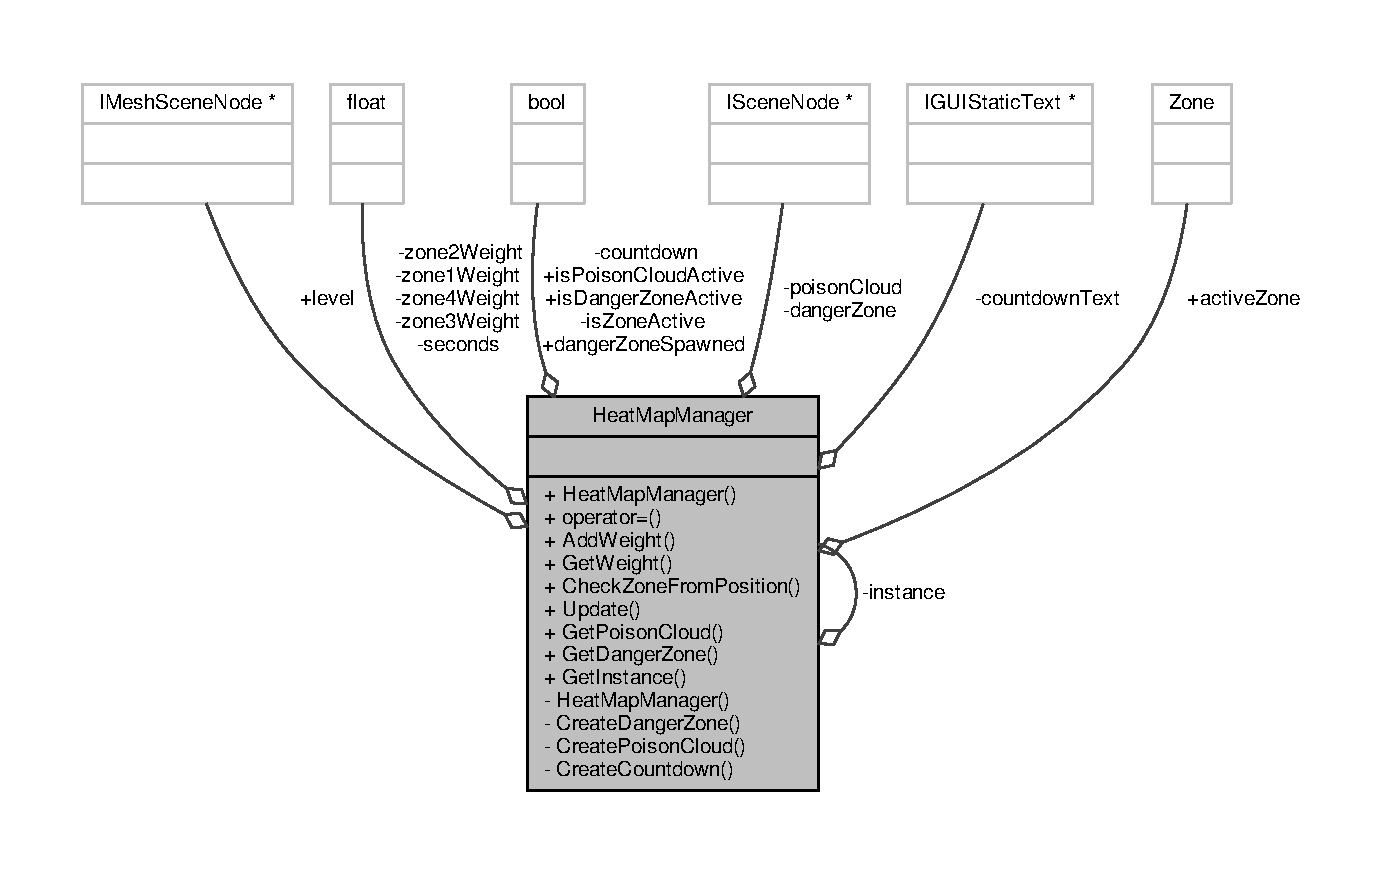
\includegraphics[width=350pt]{class_heat_map_manager__coll__graph}
\end{center}
\end{figure}
\subsection*{Public Types}
\begin{DoxyCompactItemize}
\item 
enum \hyperlink{class_heat_map_manager_a6d43bc39106e6d2e72437f8902a586b6}{Zone} \{ \\*
\hyperlink{class_heat_map_manager_a6d43bc39106e6d2e72437f8902a586b6ac37611b7d855043c25ffc9866b2145fc}{Zone0}, 
\hyperlink{class_heat_map_manager_a6d43bc39106e6d2e72437f8902a586b6ac12fb3749b1e4eb1e472927e11bfd45b}{Zone1}, 
\hyperlink{class_heat_map_manager_a6d43bc39106e6d2e72437f8902a586b6a3e20dce2afa7429facffa3cc1b41fcc3}{Zone2}, 
\hyperlink{class_heat_map_manager_a6d43bc39106e6d2e72437f8902a586b6a400a98ad8579431fad61d4325b5c9694}{Zone3}, 
\\*
\hyperlink{class_heat_map_manager_a6d43bc39106e6d2e72437f8902a586b6a39c3884e0f29b1453a01317ffc283a85}{Zone4}
 \}
\end{DoxyCompactItemize}
\subsection*{Public Member Functions}
\begin{DoxyCompactItemize}
\item 
\hyperlink{class_heat_map_manager_a572c22efd1da42802d59bd5fad291d2f}{Heat\-Map\-Manager} (const \hyperlink{class_heat_map_manager}{Heat\-Map\-Manager} \&)=delete
\item 
\hyperlink{class_heat_map_manager}{Heat\-Map\-Manager} \& \hyperlink{class_heat_map_manager_a9444c0c491587928574da5f4c2079d8c}{operator=} (const \hyperlink{class_heat_map_manager}{Heat\-Map\-Manager} \&)=delete
\item 
void \hyperlink{class_heat_map_manager_aaf3b56067a76a49a9685b221d63c87b9}{Add\-Weight} (\hyperlink{class_heat_map_manager_a6d43bc39106e6d2e72437f8902a586b6}{Zone} zone, float weight)
\item 
int \hyperlink{class_heat_map_manager_a72fbb89ab0dd5fb8b9e760f199696b16}{Get\-Weight} (\hyperlink{class_heat_map_manager_a6d43bc39106e6d2e72437f8902a586b6}{Zone} zone)
\item 
\hyperlink{class_heat_map_manager_a6d43bc39106e6d2e72437f8902a586b6}{Zone} \hyperlink{class_heat_map_manager_a13bd9841f2166a91e2f3cf93671b82f9}{Check\-Zone\-From\-Position} (irr\-::core\-::vector3df pos)
\item 
void \hyperlink{class_heat_map_manager_ac11943d3f92891670ddf9e613d7c06dd}{Update} ()
\item 
irr\-::scene\-::\-I\-Scene\-Node $\ast$ \hyperlink{class_heat_map_manager_a326372f900540856c890eb311b04876b}{Get\-Poison\-Cloud} ()
\item 
irr\-::scene\-::\-I\-Scene\-Node $\ast$ \hyperlink{class_heat_map_manager_a45ef95be18d764cedf5095ace6d87204}{Get\-Danger\-Zone} ()
\end{DoxyCompactItemize}
\subsection*{Static Public Member Functions}
\begin{DoxyCompactItemize}
\item 
static \hyperlink{class_heat_map_manager}{Heat\-Map\-Manager} $\ast$ \hyperlink{class_heat_map_manager_acc2cf6cbce0774a997ef1c408f07fb87}{Get\-Instance} ()
\end{DoxyCompactItemize}
\subsection*{Public Attributes}
\begin{DoxyCompactItemize}
\item 
irr\-::scene\-::\-I\-Mesh\-Scene\-Node $\ast$ \hyperlink{class_heat_map_manager_a63ca12aefa554bf0756608865f1e1909}{level}
\item 
\hyperlink{class_heat_map_manager_a6d43bc39106e6d2e72437f8902a586b6}{Zone} \hyperlink{class_heat_map_manager_a96bfbcb9d6326e12f37db7a9c4fd1e10}{active\-Zone}
\item 
bool \hyperlink{class_heat_map_manager_affcd194d19a8b51c54bce180d1ca2393}{is\-Poison\-Cloud\-Active} = false
\item 
bool \hyperlink{class_heat_map_manager_aa8c35fb977284623b8399a7150f68cc9}{is\-Danger\-Zone\-Active} = false
\item 
bool \hyperlink{class_heat_map_manager_a9a257b4ffed8cf8c2eaa8c71bf0fa75b}{danger\-Zone\-Spawned} = false
\end{DoxyCompactItemize}
\subsection*{Private Member Functions}
\begin{DoxyCompactItemize}
\item 
\hyperlink{class_heat_map_manager_adc7803f7074083d06bf7f2780a8943ef}{Heat\-Map\-Manager} ()
\item 
void \hyperlink{class_heat_map_manager_a5e270576638ad384789c184b0893c54d}{Create\-Danger\-Zone} (\hyperlink{class_heat_map_manager_a6d43bc39106e6d2e72437f8902a586b6}{Zone} zone)
\item 
void \hyperlink{class_heat_map_manager_a7c87473222fd1fa2acf6672a23f303a2}{Create\-Poison\-Cloud} (\hyperlink{class_heat_map_manager_a6d43bc39106e6d2e72437f8902a586b6}{Zone} zone)
\item 
void \hyperlink{class_heat_map_manager_a9c8819753979c50a6370edbd4fa6f25f}{Create\-Countdown} (\hyperlink{class_heat_map_manager_a6d43bc39106e6d2e72437f8902a586b6}{Zone} zone)
\end{DoxyCompactItemize}
\subsection*{Private Attributes}
\begin{DoxyCompactItemize}
\item 
float \hyperlink{class_heat_map_manager_a428c9124cfc0e4667e5d935fce050e3f}{zone1\-Weight}
\item 
float \hyperlink{class_heat_map_manager_a82299e638dd3f8e4c6e7cbf4706c0d0b}{zone2\-Weight}
\item 
float \hyperlink{class_heat_map_manager_aefbd0636746ab18ae5d305e4b3268ace}{zone3\-Weight}
\item 
float \hyperlink{class_heat_map_manager_a627d9bb3ce50a7473fdf84d9a048da9d}{zone4\-Weight}
\item 
bool \hyperlink{class_heat_map_manager_af53f13b64f955d297dd1d6a489ac2053}{is\-Zone\-Active} = false
\item 
bool \hyperlink{class_heat_map_manager_a659cbc23eff012306ca58bb794d9a9c1}{countdown} = false
\item 
float \hyperlink{class_heat_map_manager_a506cd0b3cef22e132ae74b5b8d264ed4}{seconds}
\item 
irr\-::scene\-::\-I\-Scene\-Node $\ast$ \hyperlink{class_heat_map_manager_a506da7726ec2f7d989ad407edd7b365d}{poison\-Cloud}
\item 
irr\-::scene\-::\-I\-Scene\-Node $\ast$ \hyperlink{class_heat_map_manager_ad5ca224ccce646f0c6fdfce6d48d1c13}{danger\-Zone}
\item 
irr\-::gui\-::\-I\-G\-U\-I\-Static\-Text $\ast$ \hyperlink{class_heat_map_manager_a6cbba801f3d09c86fa63a05180cd181e}{countdown\-Text}
\end{DoxyCompactItemize}
\subsection*{Static Private Attributes}
\begin{DoxyCompactItemize}
\item 
static \hyperlink{class_heat_map_manager}{Heat\-Map\-Manager} $\ast$ \hyperlink{class_heat_map_manager_a11d267fe86b6494e623674c2a8a8801a}{instance} = 0
\end{DoxyCompactItemize}


\subsection{Member Enumeration Documentation}
\hypertarget{class_heat_map_manager_a6d43bc39106e6d2e72437f8902a586b6}{\index{Heat\-Map\-Manager@{Heat\-Map\-Manager}!Zone@{Zone}}
\index{Zone@{Zone}!HeatMapManager@{Heat\-Map\-Manager}}
\subsubsection[{Zone}]{\setlength{\rightskip}{0pt plus 5cm}enum {\bf Heat\-Map\-Manager\-::\-Zone}}}\label{class_heat_map_manager_a6d43bc39106e6d2e72437f8902a586b6}
\begin{Desc}
\item[Enumerator]\par
\begin{description}
\index{Zone0@{Zone0}!Heat\-Map\-Manager@{Heat\-Map\-Manager}}\index{Heat\-Map\-Manager@{Heat\-Map\-Manager}!Zone0@{Zone0}}\item[{\em 
\hypertarget{class_heat_map_manager_a6d43bc39106e6d2e72437f8902a586b6ac37611b7d855043c25ffc9866b2145fc}{Zone0}\label{class_heat_map_manager_a6d43bc39106e6d2e72437f8902a586b6ac37611b7d855043c25ffc9866b2145fc}
}]\index{Zone1@{Zone1}!Heat\-Map\-Manager@{Heat\-Map\-Manager}}\index{Heat\-Map\-Manager@{Heat\-Map\-Manager}!Zone1@{Zone1}}\item[{\em 
\hypertarget{class_heat_map_manager_a6d43bc39106e6d2e72437f8902a586b6ac12fb3749b1e4eb1e472927e11bfd45b}{Zone1}\label{class_heat_map_manager_a6d43bc39106e6d2e72437f8902a586b6ac12fb3749b1e4eb1e472927e11bfd45b}
}]\index{Zone2@{Zone2}!Heat\-Map\-Manager@{Heat\-Map\-Manager}}\index{Heat\-Map\-Manager@{Heat\-Map\-Manager}!Zone2@{Zone2}}\item[{\em 
\hypertarget{class_heat_map_manager_a6d43bc39106e6d2e72437f8902a586b6a3e20dce2afa7429facffa3cc1b41fcc3}{Zone2}\label{class_heat_map_manager_a6d43bc39106e6d2e72437f8902a586b6a3e20dce2afa7429facffa3cc1b41fcc3}
}]\index{Zone3@{Zone3}!Heat\-Map\-Manager@{Heat\-Map\-Manager}}\index{Heat\-Map\-Manager@{Heat\-Map\-Manager}!Zone3@{Zone3}}\item[{\em 
\hypertarget{class_heat_map_manager_a6d43bc39106e6d2e72437f8902a586b6a400a98ad8579431fad61d4325b5c9694}{Zone3}\label{class_heat_map_manager_a6d43bc39106e6d2e72437f8902a586b6a400a98ad8579431fad61d4325b5c9694}
}]\index{Zone4@{Zone4}!Heat\-Map\-Manager@{Heat\-Map\-Manager}}\index{Heat\-Map\-Manager@{Heat\-Map\-Manager}!Zone4@{Zone4}}\item[{\em 
\hypertarget{class_heat_map_manager_a6d43bc39106e6d2e72437f8902a586b6a39c3884e0f29b1453a01317ffc283a85}{Zone4}\label{class_heat_map_manager_a6d43bc39106e6d2e72437f8902a586b6a39c3884e0f29b1453a01317ffc283a85}
}]\end{description}
\end{Desc}

\begin{DoxyCode}
12     \{
13         \hyperlink{class_heat_map_manager_a6d43bc39106e6d2e72437f8902a586b6ac37611b7d855043c25ffc9866b2145fc}{Zone0},\textcolor{comment}{//No Zone}
14         \hyperlink{class_heat_map_manager_a6d43bc39106e6d2e72437f8902a586b6ac12fb3749b1e4eb1e472927e11bfd45b}{Zone1},\textcolor{comment}{//Left-Top}
15         \hyperlink{class_heat_map_manager_a6d43bc39106e6d2e72437f8902a586b6a3e20dce2afa7429facffa3cc1b41fcc3}{Zone2},\textcolor{comment}{//Right-Top}
16         \hyperlink{class_heat_map_manager_a6d43bc39106e6d2e72437f8902a586b6a400a98ad8579431fad61d4325b5c9694}{Zone3},\textcolor{comment}{//Left-Bot}
17         \hyperlink{class_heat_map_manager_a6d43bc39106e6d2e72437f8902a586b6a39c3884e0f29b1453a01317ffc283a85}{Zone4}\textcolor{comment}{//Right-Bot}
18     \};
\end{DoxyCode}


\subsection{Constructor \& Destructor Documentation}
\hypertarget{class_heat_map_manager_a572c22efd1da42802d59bd5fad291d2f}{\index{Heat\-Map\-Manager@{Heat\-Map\-Manager}!Heat\-Map\-Manager@{Heat\-Map\-Manager}}
\index{Heat\-Map\-Manager@{Heat\-Map\-Manager}!HeatMapManager@{Heat\-Map\-Manager}}
\subsubsection[{Heat\-Map\-Manager}]{\setlength{\rightskip}{0pt plus 5cm}Heat\-Map\-Manager\-::\-Heat\-Map\-Manager (
\begin{DoxyParamCaption}
\item[{const {\bf Heat\-Map\-Manager} \&}]{}
\end{DoxyParamCaption}
)\hspace{0.3cm}{\ttfamily [delete]}}}\label{class_heat_map_manager_a572c22efd1da42802d59bd5fad291d2f}
\hypertarget{class_heat_map_manager_adc7803f7074083d06bf7f2780a8943ef}{\index{Heat\-Map\-Manager@{Heat\-Map\-Manager}!Heat\-Map\-Manager@{Heat\-Map\-Manager}}
\index{Heat\-Map\-Manager@{Heat\-Map\-Manager}!HeatMapManager@{Heat\-Map\-Manager}}
\subsubsection[{Heat\-Map\-Manager}]{\setlength{\rightskip}{0pt plus 5cm}Heat\-Map\-Manager\-::\-Heat\-Map\-Manager (
\begin{DoxyParamCaption}
{}
\end{DoxyParamCaption}
)\hspace{0.3cm}{\ttfamily [private]}}}\label{class_heat_map_manager_adc7803f7074083d06bf7f2780a8943ef}


References Sound\-Manager\-::\-Get\-Instance(), and h\-Sound\-Manager.


\begin{DoxyCode}
21 \{
22     \hyperlink{class_heat_map_manager_a428c9124cfc0e4667e5d935fce050e3f}{zone1Weight} = 0;
23     \hyperlink{class_heat_map_manager_a82299e638dd3f8e4c6e7cbf4706c0d0b}{zone2Weight} = 0;
24     \hyperlink{class_heat_map_manager_aefbd0636746ab18ae5d305e4b3268ace}{zone3Weight} = 0;
25     \hyperlink{class_heat_map_manager_a627d9bb3ce50a7473fdf84d9a048da9d}{zone4Weight} = 0;
26     \hyperlink{_heat_map_manager_8cpp_af8a1b0ce0c25e6712750f21039b8b869}{hSoundManager} = \hyperlink{_heat_map_manager_8cpp_af8a1b0ce0c25e6712750f21039b8b869}{hSoundManager}->\hyperlink{class_sound_manager_a887480b38c9380c9fba23a2337df63be}{GetInstance}();
27 \}
\end{DoxyCode}


\subsection{Member Function Documentation}
\hypertarget{class_heat_map_manager_aaf3b56067a76a49a9685b221d63c87b9}{\index{Heat\-Map\-Manager@{Heat\-Map\-Manager}!Add\-Weight@{Add\-Weight}}
\index{Add\-Weight@{Add\-Weight}!HeatMapManager@{Heat\-Map\-Manager}}
\subsubsection[{Add\-Weight}]{\setlength{\rightskip}{0pt plus 5cm}void Heat\-Map\-Manager\-::\-Add\-Weight (
\begin{DoxyParamCaption}
\item[{{\bf Zone}}]{zone, }
\item[{float}]{weight}
\end{DoxyParamCaption}
)}}\label{class_heat_map_manager_aaf3b56067a76a49a9685b221d63c87b9}


References M\-A\-X\-\_\-\-W\-E\-I\-G\-H\-T.



Referenced by Player\-::\-Move(), and Enemy\-Spawner\-::\-Update\-Enemies().


\begin{DoxyCode}
62 \{
63     \textcolor{keywordflow}{if} (\hyperlink{class_heat_map_manager_af53f13b64f955d297dd1d6a489ac2053}{isZoneActive}) \{
64         \textcolor{keywordflow}{return};
65     \}
66     \textcolor{keywordflow}{switch} (zone)
67     \{
68     \textcolor{keywordflow}{case} \hyperlink{class_heat_map_manager_a6d43bc39106e6d2e72437f8902a586b6ac12fb3749b1e4eb1e472927e11bfd45b}{Zone1}:
69         \textcolor{keywordflow}{if} (\hyperlink{class_heat_map_manager_a428c9124cfc0e4667e5d935fce050e3f}{zone1Weight} < \hyperlink{_heat_map_manager_8h_a943995a7bf30da3587664920856533ab}{MAX\_WEIGHT})
70         \{
71             \hyperlink{class_heat_map_manager_a428c9124cfc0e4667e5d935fce050e3f}{zone1Weight} += weight;
72         \}
73         \textcolor{keywordflow}{else}
74         \{
75             \hyperlink{class_heat_map_manager_a9c8819753979c50a6370edbd4fa6f25f}{CreateCountdown}(\hyperlink{class_heat_map_manager_a6d43bc39106e6d2e72437f8902a586b6ac12fb3749b1e4eb1e472927e11bfd45b}{Zone1});
76             \hyperlink{class_heat_map_manager_a428c9124cfc0e4667e5d935fce050e3f}{zone1Weight} = 0;
77         \}
78         \textcolor{keywordflow}{break};
79     \textcolor{keywordflow}{case} \hyperlink{class_heat_map_manager_a6d43bc39106e6d2e72437f8902a586b6a3e20dce2afa7429facffa3cc1b41fcc3}{Zone2}:
80         \textcolor{keywordflow}{if} (\hyperlink{class_heat_map_manager_a82299e638dd3f8e4c6e7cbf4706c0d0b}{zone2Weight} < \hyperlink{_heat_map_manager_8h_a943995a7bf30da3587664920856533ab}{MAX\_WEIGHT})
81         \{
82             \hyperlink{class_heat_map_manager_a82299e638dd3f8e4c6e7cbf4706c0d0b}{zone2Weight} += weight;
83         \}
84         \textcolor{keywordflow}{else}
85         \{
86             \hyperlink{class_heat_map_manager_a9c8819753979c50a6370edbd4fa6f25f}{CreateCountdown}(\hyperlink{class_heat_map_manager_a6d43bc39106e6d2e72437f8902a586b6a3e20dce2afa7429facffa3cc1b41fcc3}{Zone2});
87             \hyperlink{class_heat_map_manager_a82299e638dd3f8e4c6e7cbf4706c0d0b}{zone2Weight} = 0;
88         \}
89         \textcolor{keywordflow}{break};
90     \textcolor{keywordflow}{case} \hyperlink{class_heat_map_manager_a6d43bc39106e6d2e72437f8902a586b6a400a98ad8579431fad61d4325b5c9694}{Zone3}:
91         \textcolor{keywordflow}{if} (\hyperlink{class_heat_map_manager_aefbd0636746ab18ae5d305e4b3268ace}{zone3Weight} < \hyperlink{_heat_map_manager_8h_a943995a7bf30da3587664920856533ab}{MAX\_WEIGHT})
92         \{
93             \hyperlink{class_heat_map_manager_aefbd0636746ab18ae5d305e4b3268ace}{zone3Weight} += weight;
94         \}
95         \textcolor{keywordflow}{else}
96         \{
97             \hyperlink{class_heat_map_manager_a9c8819753979c50a6370edbd4fa6f25f}{CreateCountdown}(\hyperlink{class_heat_map_manager_a6d43bc39106e6d2e72437f8902a586b6a400a98ad8579431fad61d4325b5c9694}{Zone3});
98             \hyperlink{class_heat_map_manager_aefbd0636746ab18ae5d305e4b3268ace}{zone3Weight} = 0;
99         \}
100         \textcolor{keywordflow}{break};
101     \textcolor{keywordflow}{case} \hyperlink{class_heat_map_manager_a6d43bc39106e6d2e72437f8902a586b6a39c3884e0f29b1453a01317ffc283a85}{Zone4}:
102         \textcolor{keywordflow}{if} (\hyperlink{class_heat_map_manager_a627d9bb3ce50a7473fdf84d9a048da9d}{zone4Weight} < \hyperlink{_heat_map_manager_8h_a943995a7bf30da3587664920856533ab}{MAX\_WEIGHT})
103         \{
104             \hyperlink{class_heat_map_manager_a627d9bb3ce50a7473fdf84d9a048da9d}{zone4Weight} += weight;
105         \}
106         \textcolor{keywordflow}{else}
107         \{
108             \hyperlink{class_heat_map_manager_a9c8819753979c50a6370edbd4fa6f25f}{CreateCountdown}(\hyperlink{class_heat_map_manager_a6d43bc39106e6d2e72437f8902a586b6a39c3884e0f29b1453a01317ffc283a85}{Zone4});
109             \hyperlink{class_heat_map_manager_a627d9bb3ce50a7473fdf84d9a048da9d}{zone4Weight} = 0;
110         \}
111         \textcolor{keywordflow}{break};
112     \textcolor{keywordflow}{default}:
113         \textcolor{keywordflow}{break};
114     \}
115 \}
\end{DoxyCode}
\hypertarget{class_heat_map_manager_a13bd9841f2166a91e2f3cf93671b82f9}{\index{Heat\-Map\-Manager@{Heat\-Map\-Manager}!Check\-Zone\-From\-Position@{Check\-Zone\-From\-Position}}
\index{Check\-Zone\-From\-Position@{Check\-Zone\-From\-Position}!HeatMapManager@{Heat\-Map\-Manager}}
\subsubsection[{Check\-Zone\-From\-Position}]{\setlength{\rightskip}{0pt plus 5cm}{\bf Heat\-Map\-Manager\-::\-Zone} Heat\-Map\-Manager\-::\-Check\-Zone\-From\-Position (
\begin{DoxyParamCaption}
\item[{irr\-::core\-::vector3df}]{pos}
\end{DoxyParamCaption}
)}}\label{class_heat_map_manager_a13bd9841f2166a91e2f3cf93671b82f9}


Referenced by Player\-::\-Move(), and Enemy\-Spawner\-::\-Update\-Enemies().


\begin{DoxyCode}
42 \{
43     \textcolor{keywordflow}{if} (pos.X > 0 && pos.Z > 0)
44     \{
45         \textcolor{keywordflow}{return} \hyperlink{class_heat_map_manager_a6d43bc39106e6d2e72437f8902a586b6ac12fb3749b1e4eb1e472927e11bfd45b}{Zone1};
46     \}
47     \textcolor{keywordflow}{else} \textcolor{keywordflow}{if} (pos.X > 0 && pos.Z < 0)
48     \{
49         \textcolor{keywordflow}{return} \hyperlink{class_heat_map_manager_a6d43bc39106e6d2e72437f8902a586b6a3e20dce2afa7429facffa3cc1b41fcc3}{Zone2};
50     \}
51     \textcolor{keywordflow}{else} \textcolor{keywordflow}{if} (pos.X < 0 && pos.Z > 0)
52     \{
53         \textcolor{keywordflow}{return} \hyperlink{class_heat_map_manager_a6d43bc39106e6d2e72437f8902a586b6a400a98ad8579431fad61d4325b5c9694}{Zone3};
54     \}
55     \textcolor{keywordflow}{else} \textcolor{keywordflow}{if} (pos.X < 0 && pos.Z < 0)
56     \{
57         \textcolor{keywordflow}{return} \hyperlink{class_heat_map_manager_a6d43bc39106e6d2e72437f8902a586b6a39c3884e0f29b1453a01317ffc283a85}{Zone4};
58     \}
59 \}
\end{DoxyCode}
\hypertarget{class_heat_map_manager_a9c8819753979c50a6370edbd4fa6f25f}{\index{Heat\-Map\-Manager@{Heat\-Map\-Manager}!Create\-Countdown@{Create\-Countdown}}
\index{Create\-Countdown@{Create\-Countdown}!HeatMapManager@{Heat\-Map\-Manager}}
\subsubsection[{Create\-Countdown}]{\setlength{\rightskip}{0pt plus 5cm}void Heat\-Map\-Manager\-::\-Create\-Countdown (
\begin{DoxyParamCaption}
\item[{{\bf Zone}}]{zone}
\end{DoxyParamCaption}
)\hspace{0.3cm}{\ttfamily [private]}}}\label{class_heat_map_manager_a9c8819753979c50a6370edbd4fa6f25f}


References M\-A\-X\-\_\-\-C\-O\-U\-N\-T\-D\-O\-W\-N\-\_\-\-S\-E\-C\-O\-N\-D\-S, and ui.


\begin{DoxyCode}
188 \{
189     \hyperlink{class_heat_map_manager_af53f13b64f955d297dd1d6a489ac2053}{isZoneActive} = \textcolor{keyword}{true};
190     \hyperlink{class_heat_map_manager_a659cbc23eff012306ca58bb794d9a9c1}{countdown} = \textcolor{keyword}{true};
191     \hyperlink{class_heat_map_manager_a96bfbcb9d6326e12f37db7a9c4fd1e10}{activeZone} = zone;
192     stringw text(\textcolor{stringliteral}{"There will be gas in Zone "});
193     text += zone;
194     text += \textcolor{stringliteral}{" in 5 seconds"};
195     \hyperlink{class_heat_map_manager_a6cbba801f3d09c86fa63a05180cd181e}{countdownText} = \hyperlink{_heat_map_manager_8cpp_aba421c4a07fe59ce15705794f2fa8eaf}{ui}->addStaticText(text.c\_str(), rect<int>(350, 80, 450, 120), \textcolor{keyword}{true}, \textcolor{keyword}{true}
      , 0, -1, \textcolor{keyword}{true});
196     \hyperlink{class_heat_map_manager_a6cbba801f3d09c86fa63a05180cd181e}{countdownText}->setMinSize(dimension2du(100, 40));
197     \hyperlink{class_heat_map_manager_a6cbba801f3d09c86fa63a05180cd181e}{countdownText}->setMaxSize(dimension2du(100, 40));
198 
199     \hyperlink{class_heat_map_manager_a506cd0b3cef22e132ae74b5b8d264ed4}{seconds} = \hyperlink{_heat_map_manager_8h_ab0e3989937f8f286cd67309cf671a477}{MAX\_COUNTDOWN\_SECONDS};
200 \}
\end{DoxyCode}
\hypertarget{class_heat_map_manager_a5e270576638ad384789c184b0893c54d}{\index{Heat\-Map\-Manager@{Heat\-Map\-Manager}!Create\-Danger\-Zone@{Create\-Danger\-Zone}}
\index{Create\-Danger\-Zone@{Create\-Danger\-Zone}!HeatMapManager@{Heat\-Map\-Manager}}
\subsubsection[{Create\-Danger\-Zone}]{\setlength{\rightskip}{0pt plus 5cm}void Heat\-Map\-Manager\-::\-Create\-Danger\-Zone (
\begin{DoxyParamCaption}
\item[{{\bf Zone}}]{zone}
\end{DoxyParamCaption}
)\hspace{0.3cm}{\ttfamily [private]}}}\label{class_heat_map_manager_a5e270576638ad384789c184b0893c54d}


References Game\-::device, h\-Game, and hsmgr.


\begin{DoxyCode}
202 \{
203     \textcolor{keyword}{const} path texturePathDangerZone = \textcolor{stringliteral}{"../media/Textures/danger\_texture.png"};
204     vector3df dangerZonePosition;
205     dangerZonePosition.Y = -1.5;
206     f32 size = \hyperlink{class_heat_map_manager_a63ca12aefa554bf0756608865f1e1909}{level}->getTransformedBoundingBox().getExtent().X / 18;
207     \textcolor{keywordflow}{switch} (zone)
208     \{
209     \textcolor{keywordflow}{case} \hyperlink{class_heat_map_manager_a6d43bc39106e6d2e72437f8902a586b6ac12fb3749b1e4eb1e472927e11bfd45b}{Zone1}:
210         dangerZonePosition.X = size;
211         dangerZonePosition.Z = size;
212         \textcolor{keywordflow}{break};
213     \textcolor{keywordflow}{case} \hyperlink{class_heat_map_manager_a6d43bc39106e6d2e72437f8902a586b6a3e20dce2afa7429facffa3cc1b41fcc3}{Zone2}:
214         dangerZonePosition.X = size;
215         dangerZonePosition.Z = -size;
216         \textcolor{keywordflow}{break};
217     \textcolor{keywordflow}{case} \hyperlink{class_heat_map_manager_a6d43bc39106e6d2e72437f8902a586b6a400a98ad8579431fad61d4325b5c9694}{Zone3}:
218         dangerZonePosition.X = -size;
219         dangerZonePosition.Z = size;
220         \textcolor{keywordflow}{break};
221     \textcolor{keywordflow}{case} \hyperlink{class_heat_map_manager_a6d43bc39106e6d2e72437f8902a586b6a39c3884e0f29b1453a01317ffc283a85}{Zone4}:
222         dangerZonePosition.X = -size;
223         dangerZonePosition.Z = -size;
224         \textcolor{keywordflow}{break};
225     \textcolor{keywordflow}{default}:
226         \textcolor{keywordflow}{break};
227     \}
228     dangerZonePosition.X *= 5;
229     dangerZonePosition.Z *= 5;
230     \hyperlink{class_heat_map_manager_ad5ca224ccce646f0c6fdfce6d48d1c13}{dangerZone} = \hyperlink{_heat_map_manager_8cpp_afce8176d06e37bb8d8bf11f5947b4181}{hsmgr}->addCubeSceneNode();
231     \textcolor{keywordflow}{if} (\hyperlink{class_heat_map_manager_ad5ca224ccce646f0c6fdfce6d48d1c13}{dangerZone}) \{
232         \hyperlink{class_heat_map_manager_ad5ca224ccce646f0c6fdfce6d48d1c13}{dangerZone}->setPosition(dangerZonePosition);
233         \hyperlink{class_heat_map_manager_ad5ca224ccce646f0c6fdfce6d48d1c13}{dangerZone}->setScale(vector3df(size, 0.4f, size));
234 
235         \hyperlink{class_heat_map_manager_ad5ca224ccce646f0c6fdfce6d48d1c13}{dangerZone}->setMaterialFlag(video::EMF\_LIGHTING, \textcolor{keyword}{false});
236         \hyperlink{class_heat_map_manager_ad5ca224ccce646f0c6fdfce6d48d1c13}{dangerZone}->setMaterialFlag(video::EMF\_ZWRITE\_ENABLE, \textcolor{keyword}{false});
237         \hyperlink{class_heat_map_manager_ad5ca224ccce646f0c6fdfce6d48d1c13}{dangerZone}->setMaterialTexture(0, \hyperlink{_heat_map_manager_8cpp_ac34ec415c121b1595d2b5d4b545ae96b}{hGame}->\hyperlink{class_game_a4968552e2ba3037d494596a908eccc00}{device}->getVideoDriver()->getTexture(
      texturePathDangerZone));
238         \hyperlink{class_heat_map_manager_ad5ca224ccce646f0c6fdfce6d48d1c13}{dangerZone}->setMaterialType(video::EMT\_TRANSPARENT\_ADD\_COLOR);
239     \}
240     \textcolor{comment}{//isDangerZoneActive = true;}
241 \}
\end{DoxyCode}
\hypertarget{class_heat_map_manager_a7c87473222fd1fa2acf6672a23f303a2}{\index{Heat\-Map\-Manager@{Heat\-Map\-Manager}!Create\-Poison\-Cloud@{Create\-Poison\-Cloud}}
\index{Create\-Poison\-Cloud@{Create\-Poison\-Cloud}!HeatMapManager@{Heat\-Map\-Manager}}
\subsubsection[{Create\-Poison\-Cloud}]{\setlength{\rightskip}{0pt plus 5cm}void Heat\-Map\-Manager\-::\-Create\-Poison\-Cloud (
\begin{DoxyParamCaption}
\item[{{\bf Zone}}]{zone}
\end{DoxyParamCaption}
)\hspace{0.3cm}{\ttfamily [private]}}}\label{class_heat_map_manager_a7c87473222fd1fa2acf6672a23f303a2}


References Game\-::device, G\-A\-S\-\_\-\-S\-O\-U\-N\-D, h\-Game, hsmgr, h\-Sound\-Manager, M\-A\-X\-\_\-\-P\-O\-I\-S\-O\-N\-C\-L\-O\-U\-S\-\_\-\-S\-E\-C\-O\-N\-D\-S, and Sound\-Manager\-::\-Play\-Sound().


\begin{DoxyCode}
244 \{
245     \textcolor{comment}{//const path texturePathDangerZone = "../media/Textures/danger\_texture.png";}
246     \textcolor{keyword}{const} path texturePath = \textcolor{stringliteral}{"../media/Textures/PoisonCloud.jpg"};
247     vector3df cloudPosition;
248     cloudPosition.Y = -0.5;
249     f32 size = \hyperlink{class_heat_map_manager_a63ca12aefa554bf0756608865f1e1909}{level}->getTransformedBoundingBox().getExtent().X / 18;
250     \textcolor{keywordflow}{switch} (zone)
251     \{
252     \textcolor{keywordflow}{case} \hyperlink{class_heat_map_manager_a6d43bc39106e6d2e72437f8902a586b6ac12fb3749b1e4eb1e472927e11bfd45b}{Zone1}:
253         cloudPosition.X = size;
254         cloudPosition.Z = size;
255         \textcolor{keywordflow}{break};
256     \textcolor{keywordflow}{case} \hyperlink{class_heat_map_manager_a6d43bc39106e6d2e72437f8902a586b6a3e20dce2afa7429facffa3cc1b41fcc3}{Zone2}:
257         cloudPosition.X = size;
258         cloudPosition.Z = -size;
259         \textcolor{keywordflow}{break};
260     \textcolor{keywordflow}{case} \hyperlink{class_heat_map_manager_a6d43bc39106e6d2e72437f8902a586b6a400a98ad8579431fad61d4325b5c9694}{Zone3}:
261         cloudPosition.X = -size;
262         cloudPosition.Z = size;
263         \textcolor{keywordflow}{break};
264     \textcolor{keywordflow}{case} \hyperlink{class_heat_map_manager_a6d43bc39106e6d2e72437f8902a586b6a39c3884e0f29b1453a01317ffc283a85}{Zone4}:
265         cloudPosition.X = -size;
266         cloudPosition.Z = -size;
267         \textcolor{keywordflow}{break};
268     \textcolor{keywordflow}{default}:
269         \textcolor{keywordflow}{break};
270     \}
271     cloudPosition.X *= 5;
272     cloudPosition.Z *= 5;
273     \hyperlink{class_heat_map_manager_a506da7726ec2f7d989ad407edd7b365d}{poisonCloud} = \hyperlink{_heat_map_manager_8cpp_afce8176d06e37bb8d8bf11f5947b4181}{hsmgr}->addCubeSceneNode();
274     \textcolor{keywordflow}{if} (\hyperlink{class_heat_map_manager_a506da7726ec2f7d989ad407edd7b365d}{poisonCloud}) \{
275         \hyperlink{class_heat_map_manager_a506da7726ec2f7d989ad407edd7b365d}{poisonCloud}->setPosition(cloudPosition);
276         \hyperlink{class_heat_map_manager_a506da7726ec2f7d989ad407edd7b365d}{poisonCloud}->setScale(vector3df(size, 4.0, size));
277 
278         \hyperlink{class_heat_map_manager_a506da7726ec2f7d989ad407edd7b365d}{poisonCloud}->setMaterialFlag(video::EMF\_LIGHTING, \textcolor{keyword}{false});
279         \hyperlink{class_heat_map_manager_a506da7726ec2f7d989ad407edd7b365d}{poisonCloud}->setMaterialFlag(video::EMF\_ZWRITE\_ENABLE, \textcolor{keyword}{false});
280         \hyperlink{class_heat_map_manager_a506da7726ec2f7d989ad407edd7b365d}{poisonCloud}->setMaterialTexture(0, \hyperlink{_heat_map_manager_8cpp_ac34ec415c121b1595d2b5d4b545ae96b}{hGame}->\hyperlink{class_game_a4968552e2ba3037d494596a908eccc00}{device}->getVideoDriver()->
      getTexture(texturePath));
281         \hyperlink{class_heat_map_manager_a506da7726ec2f7d989ad407edd7b365d}{poisonCloud}->setMaterialType(video::EMT\_TRANSPARENT\_ADD\_COLOR);
282     \}
283     \hyperlink{class_heat_map_manager_affcd194d19a8b51c54bce180d1ca2393}{isPoisonCloudActive} = \textcolor{keyword}{true};
284     \hyperlink{class_heat_map_manager_a506cd0b3cef22e132ae74b5b8d264ed4}{seconds} = \hyperlink{_heat_map_manager_8h_a2060785d16be1e99ba8c9a508799c641}{MAX\_POISONCLOUS\_SECONDS};
285     \hyperlink{_heat_map_manager_8cpp_af8a1b0ce0c25e6712750f21039b8b869}{hSoundManager}->\hyperlink{class_sound_manager_a81e8f88fe549f6767d3552f12c28ecbc}{PlaySound}(\hyperlink{_heat_map_manager_8h_aac873f74ed04299cc7b7f1f4a6f61100}{GAS\_SOUND}, \textcolor{keyword}{false});
286 \}
\end{DoxyCode}
\hypertarget{class_heat_map_manager_a45ef95be18d764cedf5095ace6d87204}{\index{Heat\-Map\-Manager@{Heat\-Map\-Manager}!Get\-Danger\-Zone@{Get\-Danger\-Zone}}
\index{Get\-Danger\-Zone@{Get\-Danger\-Zone}!HeatMapManager@{Heat\-Map\-Manager}}
\subsubsection[{Get\-Danger\-Zone}]{\setlength{\rightskip}{0pt plus 5cm}I\-Scene\-Node $\ast$ Heat\-Map\-Manager\-::\-Get\-Danger\-Zone (
\begin{DoxyParamCaption}
{}
\end{DoxyParamCaption}
)}}\label{class_heat_map_manager_a45ef95be18d764cedf5095ace6d87204}

\begin{DoxyCode}
288                                           \{
289     \textcolor{keywordflow}{return} \hyperlink{class_heat_map_manager_ad5ca224ccce646f0c6fdfce6d48d1c13}{dangerZone};
290 \}
\end{DoxyCode}
\hypertarget{class_heat_map_manager_acc2cf6cbce0774a997ef1c408f07fb87}{\index{Heat\-Map\-Manager@{Heat\-Map\-Manager}!Get\-Instance@{Get\-Instance}}
\index{Get\-Instance@{Get\-Instance}!HeatMapManager@{Heat\-Map\-Manager}}
\subsubsection[{Get\-Instance}]{\setlength{\rightskip}{0pt plus 5cm}{\bf Heat\-Map\-Manager} $\ast$ Heat\-Map\-Manager\-::\-Get\-Instance (
\begin{DoxyParamCaption}
{}
\end{DoxyParamCaption}
)\hspace{0.3cm}{\ttfamily [static]}}}\label{class_heat_map_manager_acc2cf6cbce0774a997ef1c408f07fb87}


Referenced by Object\-Placement\-Generation\-::\-Create\-Default\-Objects(), and Enemy\-Spawner\-::\-Enemy\-Spawner().


\begin{DoxyCode}
33 \{
34     \textcolor{keywordflow}{if} (!\hyperlink{class_heat_map_manager_a11d267fe86b6494e623674c2a8a8801a}{instance})
35     \{
36         \hyperlink{class_heat_map_manager_a11d267fe86b6494e623674c2a8a8801a}{instance} = \textcolor{keyword}{new} \hyperlink{class_heat_map_manager_adc7803f7074083d06bf7f2780a8943ef}{HeatMapManager}();
37     \}
38     \textcolor{keywordflow}{return} \hyperlink{class_heat_map_manager_a11d267fe86b6494e623674c2a8a8801a}{instance};
39 \}
\end{DoxyCode}
\hypertarget{class_heat_map_manager_a326372f900540856c890eb311b04876b}{\index{Heat\-Map\-Manager@{Heat\-Map\-Manager}!Get\-Poison\-Cloud@{Get\-Poison\-Cloud}}
\index{Get\-Poison\-Cloud@{Get\-Poison\-Cloud}!HeatMapManager@{Heat\-Map\-Manager}}
\subsubsection[{Get\-Poison\-Cloud}]{\setlength{\rightskip}{0pt plus 5cm}I\-Scene\-Node $\ast$ Heat\-Map\-Manager\-::\-Get\-Poison\-Cloud (
\begin{DoxyParamCaption}
{}
\end{DoxyParamCaption}
)}}\label{class_heat_map_manager_a326372f900540856c890eb311b04876b}

\begin{DoxyCode}
292                                            \{
293     \textcolor{keywordflow}{return} \hyperlink{class_heat_map_manager_a506da7726ec2f7d989ad407edd7b365d}{poisonCloud};
294 \}
\end{DoxyCode}
\hypertarget{class_heat_map_manager_a72fbb89ab0dd5fb8b9e760f199696b16}{\index{Heat\-Map\-Manager@{Heat\-Map\-Manager}!Get\-Weight@{Get\-Weight}}
\index{Get\-Weight@{Get\-Weight}!HeatMapManager@{Heat\-Map\-Manager}}
\subsubsection[{Get\-Weight}]{\setlength{\rightskip}{0pt plus 5cm}int Heat\-Map\-Manager\-::\-Get\-Weight (
\begin{DoxyParamCaption}
\item[{{\bf Zone}}]{zone}
\end{DoxyParamCaption}
)}}\label{class_heat_map_manager_a72fbb89ab0dd5fb8b9e760f199696b16}

\begin{DoxyCode}
118 \{
119     \textcolor{keywordflow}{switch} (zone)
120     \{
121     \textcolor{keywordflow}{case} \hyperlink{class_heat_map_manager_a6d43bc39106e6d2e72437f8902a586b6ac12fb3749b1e4eb1e472927e11bfd45b}{Zone1}:
122         \textcolor{keywordflow}{return} \hyperlink{class_heat_map_manager_a428c9124cfc0e4667e5d935fce050e3f}{zone1Weight};
123         \textcolor{keywordflow}{break};
124     \textcolor{keywordflow}{case} \hyperlink{class_heat_map_manager_a6d43bc39106e6d2e72437f8902a586b6a3e20dce2afa7429facffa3cc1b41fcc3}{Zone2}:
125         \textcolor{keywordflow}{return} \hyperlink{class_heat_map_manager_a82299e638dd3f8e4c6e7cbf4706c0d0b}{zone2Weight};
126         \textcolor{keywordflow}{break};
127     \textcolor{keywordflow}{case} \hyperlink{class_heat_map_manager_a6d43bc39106e6d2e72437f8902a586b6a400a98ad8579431fad61d4325b5c9694}{Zone3}:
128         \textcolor{keywordflow}{return} \hyperlink{class_heat_map_manager_aefbd0636746ab18ae5d305e4b3268ace}{zone3Weight};
129         \textcolor{keywordflow}{break};
130     \textcolor{keywordflow}{case} \hyperlink{class_heat_map_manager_a6d43bc39106e6d2e72437f8902a586b6a39c3884e0f29b1453a01317ffc283a85}{Zone4}:
131         \textcolor{keywordflow}{return} \hyperlink{class_heat_map_manager_a627d9bb3ce50a7473fdf84d9a048da9d}{zone4Weight};
132         \textcolor{keywordflow}{break};
133     \textcolor{keywordflow}{default}:
134         \textcolor{keywordflow}{break};
135     \}
136 \}
\end{DoxyCode}
\hypertarget{class_heat_map_manager_a9444c0c491587928574da5f4c2079d8c}{\index{Heat\-Map\-Manager@{Heat\-Map\-Manager}!operator=@{operator=}}
\index{operator=@{operator=}!HeatMapManager@{Heat\-Map\-Manager}}
\subsubsection[{operator=}]{\setlength{\rightskip}{0pt plus 5cm}{\bf Heat\-Map\-Manager}\& Heat\-Map\-Manager\-::operator= (
\begin{DoxyParamCaption}
\item[{const {\bf Heat\-Map\-Manager} \&}]{}
\end{DoxyParamCaption}
)\hspace{0.3cm}{\ttfamily [delete]}}}\label{class_heat_map_manager_a9444c0c491587928574da5f4c2079d8c}
\hypertarget{class_heat_map_manager_ac11943d3f92891670ddf9e613d7c06dd}{\index{Heat\-Map\-Manager@{Heat\-Map\-Manager}!Update@{Update}}
\index{Update@{Update}!HeatMapManager@{Heat\-Map\-Manager}}
\subsubsection[{Update}]{\setlength{\rightskip}{0pt plus 5cm}void Heat\-Map\-Manager\-::\-Update (
\begin{DoxyParamCaption}
{}
\end{DoxyParamCaption}
)}}\label{class_heat_map_manager_ac11943d3f92891670ddf9e613d7c06dd}


References Object\-Placement\-Generation\-::\-Generate\-New\-Objects(), h\-Game, hsmgr, and Game\-::object\-Placement\-Gen.



Referenced by Player\-::\-Move().


\begin{DoxyCode}
139 \{
140     \textcolor{keywordflow}{if} (\hyperlink{class_heat_map_manager_a659cbc23eff012306ca58bb794d9a9c1}{countdown})
141     \{
142         \hyperlink{class_heat_map_manager_a506cd0b3cef22e132ae74b5b8d264ed4}{seconds} -= 0.016; \textcolor{comment}{//we use vsync, so it's always 60fps, 0.016 is the framedeltatime}
143         stringw newText(\textcolor{stringliteral}{"There will be gas in Zone "});
144         newText += \hyperlink{class_heat_map_manager_a96bfbcb9d6326e12f37db7a9c4fd1e10}{activeZone};
145         newText += \textcolor{stringliteral}{" in "};
146         newText += \hyperlink{class_heat_map_manager_a506cd0b3cef22e132ae74b5b8d264ed4}{seconds};
147         newText += \textcolor{stringliteral}{" seconds"};
148         \hyperlink{class_heat_map_manager_a6cbba801f3d09c86fa63a05180cd181e}{countdownText}->setText(newText.c\_str());
149 
150         \hyperlink{class_heat_map_manager_aa8c35fb977284623b8399a7150f68cc9}{isDangerZoneActive} = \textcolor{keyword}{true};
151         \textcolor{keywordflow}{if} (\hyperlink{class_heat_map_manager_a506cd0b3cef22e132ae74b5b8d264ed4}{seconds} < 0)
152         \{
153             \hyperlink{class_heat_map_manager_a659cbc23eff012306ca58bb794d9a9c1}{countdown} = \textcolor{keyword}{false};
154             \hyperlink{class_heat_map_manager_a7c87473222fd1fa2acf6672a23f303a2}{CreatePoisonCloud}(\hyperlink{class_heat_map_manager_a96bfbcb9d6326e12f37db7a9c4fd1e10}{activeZone});
155             \hyperlink{class_heat_map_manager_a6cbba801f3d09c86fa63a05180cd181e}{countdownText}->remove();
156         \}
157     \}
158     \textcolor{keywordflow}{if} (\hyperlink{class_heat_map_manager_aa8c35fb977284623b8399a7150f68cc9}{isDangerZoneActive} && \hyperlink{class_heat_map_manager_a9a257b4ffed8cf8c2eaa8c71bf0fa75b}{dangerZoneSpawned} == \textcolor{keyword}{false})
159     \{
160         \hyperlink{class_heat_map_manager_a5e270576638ad384789c184b0893c54d}{CreateDangerZone}(\hyperlink{class_heat_map_manager_a96bfbcb9d6326e12f37db7a9c4fd1e10}{activeZone});
161         \hyperlink{class_heat_map_manager_a9a257b4ffed8cf8c2eaa8c71bf0fa75b}{dangerZoneSpawned} = \textcolor{keyword}{true};
162         \textcolor{comment}{//isDangerZoneActive = false;}
163     \}
164     \textcolor{keywordflow}{if} (\hyperlink{class_heat_map_manager_affcd194d19a8b51c54bce180d1ca2393}{isPoisonCloudActive})
165     \{
166         \textcolor{keywordflow}{if} (\hyperlink{class_heat_map_manager_aa8c35fb977284623b8399a7150f68cc9}{isDangerZoneActive})
167         \{
168             \hyperlink{class_heat_map_manager_aa8c35fb977284623b8399a7150f68cc9}{isDangerZoneActive} = \textcolor{keyword}{false};
169             \hyperlink{class_heat_map_manager_a9a257b4ffed8cf8c2eaa8c71bf0fa75b}{dangerZoneSpawned} = \textcolor{keyword}{false};
170             \textcolor{comment}{//dangerZone->remove();}
171             \hyperlink{_heat_map_manager_8cpp_afce8176d06e37bb8d8bf11f5947b4181}{hsmgr}->addToDeletionQueue(\hyperlink{class_heat_map_manager_a45ef95be18d764cedf5095ace6d87204}{GetDangerZone}());
172         \}
173         \textcolor{comment}{//hsmgr->addToDeletionQueue(GetDangerZone());  <--- HERE's THE ERROR }
174         \hyperlink{class_heat_map_manager_a506cd0b3cef22e132ae74b5b8d264ed4}{seconds} -= 0.016;
175         \textcolor{keywordflow}{if} (\hyperlink{class_heat_map_manager_a506cd0b3cef22e132ae74b5b8d264ed4}{seconds} < 0)
176         \{
177             \hyperlink{_heat_map_manager_8cpp_ac34ec415c121b1595d2b5d4b545ae96b}{hGame}->\hyperlink{class_game_a582b0adfa98534d79ec9511919827029}{objectPlacementGen}.\hyperlink{class_object_placement_generation_aba7072b3fd4c0443ec7884b108b8847a}{GenerateNewObjects}(
      \hyperlink{class_heat_map_manager_a96bfbcb9d6326e12f37db7a9c4fd1e10}{activeZone});
178             \hyperlink{_heat_map_manager_8cpp_afce8176d06e37bb8d8bf11f5947b4181}{hsmgr}->addToDeletionQueue(\hyperlink{class_heat_map_manager_a326372f900540856c890eb311b04876b}{GetPoisonCloud}());
179             \textcolor{comment}{//poisonCloud->setVisible(false);}
180             \hyperlink{class_heat_map_manager_af53f13b64f955d297dd1d6a489ac2053}{isZoneActive} = \textcolor{keyword}{false};
181             \hyperlink{class_heat_map_manager_affcd194d19a8b51c54bce180d1ca2393}{isPoisonCloudActive} = \textcolor{keyword}{false};
182             \hyperlink{class_heat_map_manager_a96bfbcb9d6326e12f37db7a9c4fd1e10}{activeZone} = \hyperlink{class_heat_map_manager_a6d43bc39106e6d2e72437f8902a586b6ac37611b7d855043c25ffc9866b2145fc}{Zone0};
183         \}
184     \}
185 \}
\end{DoxyCode}


\subsection{Member Data Documentation}
\hypertarget{class_heat_map_manager_a96bfbcb9d6326e12f37db7a9c4fd1e10}{\index{Heat\-Map\-Manager@{Heat\-Map\-Manager}!active\-Zone@{active\-Zone}}
\index{active\-Zone@{active\-Zone}!HeatMapManager@{Heat\-Map\-Manager}}
\subsubsection[{active\-Zone}]{\setlength{\rightskip}{0pt plus 5cm}{\bf Zone} Heat\-Map\-Manager\-::active\-Zone}}\label{class_heat_map_manager_a96bfbcb9d6326e12f37db7a9c4fd1e10}


Referenced by Player\-::\-Move().

\hypertarget{class_heat_map_manager_a659cbc23eff012306ca58bb794d9a9c1}{\index{Heat\-Map\-Manager@{Heat\-Map\-Manager}!countdown@{countdown}}
\index{countdown@{countdown}!HeatMapManager@{Heat\-Map\-Manager}}
\subsubsection[{countdown}]{\setlength{\rightskip}{0pt plus 5cm}bool Heat\-Map\-Manager\-::countdown = false\hspace{0.3cm}{\ttfamily [private]}}}\label{class_heat_map_manager_a659cbc23eff012306ca58bb794d9a9c1}
\hypertarget{class_heat_map_manager_a6cbba801f3d09c86fa63a05180cd181e}{\index{Heat\-Map\-Manager@{Heat\-Map\-Manager}!countdown\-Text@{countdown\-Text}}
\index{countdown\-Text@{countdown\-Text}!HeatMapManager@{Heat\-Map\-Manager}}
\subsubsection[{countdown\-Text}]{\setlength{\rightskip}{0pt plus 5cm}irr\-::gui\-::\-I\-G\-U\-I\-Static\-Text$\ast$ Heat\-Map\-Manager\-::countdown\-Text\hspace{0.3cm}{\ttfamily [private]}}}\label{class_heat_map_manager_a6cbba801f3d09c86fa63a05180cd181e}
\hypertarget{class_heat_map_manager_ad5ca224ccce646f0c6fdfce6d48d1c13}{\index{Heat\-Map\-Manager@{Heat\-Map\-Manager}!danger\-Zone@{danger\-Zone}}
\index{danger\-Zone@{danger\-Zone}!HeatMapManager@{Heat\-Map\-Manager}}
\subsubsection[{danger\-Zone}]{\setlength{\rightskip}{0pt plus 5cm}irr\-::scene\-::\-I\-Scene\-Node$\ast$ Heat\-Map\-Manager\-::danger\-Zone\hspace{0.3cm}{\ttfamily [private]}}}\label{class_heat_map_manager_ad5ca224ccce646f0c6fdfce6d48d1c13}
\hypertarget{class_heat_map_manager_a9a257b4ffed8cf8c2eaa8c71bf0fa75b}{\index{Heat\-Map\-Manager@{Heat\-Map\-Manager}!danger\-Zone\-Spawned@{danger\-Zone\-Spawned}}
\index{danger\-Zone\-Spawned@{danger\-Zone\-Spawned}!HeatMapManager@{Heat\-Map\-Manager}}
\subsubsection[{danger\-Zone\-Spawned}]{\setlength{\rightskip}{0pt plus 5cm}bool Heat\-Map\-Manager\-::danger\-Zone\-Spawned = false}}\label{class_heat_map_manager_a9a257b4ffed8cf8c2eaa8c71bf0fa75b}
\hypertarget{class_heat_map_manager_a11d267fe86b6494e623674c2a8a8801a}{\index{Heat\-Map\-Manager@{Heat\-Map\-Manager}!instance@{instance}}
\index{instance@{instance}!HeatMapManager@{Heat\-Map\-Manager}}
\subsubsection[{instance}]{\setlength{\rightskip}{0pt plus 5cm}{\bf Heat\-Map\-Manager} $\ast$ Heat\-Map\-Manager\-::instance = 0\hspace{0.3cm}{\ttfamily [static]}, {\ttfamily [private]}}}\label{class_heat_map_manager_a11d267fe86b6494e623674c2a8a8801a}
\hypertarget{class_heat_map_manager_aa8c35fb977284623b8399a7150f68cc9}{\index{Heat\-Map\-Manager@{Heat\-Map\-Manager}!is\-Danger\-Zone\-Active@{is\-Danger\-Zone\-Active}}
\index{is\-Danger\-Zone\-Active@{is\-Danger\-Zone\-Active}!HeatMapManager@{Heat\-Map\-Manager}}
\subsubsection[{is\-Danger\-Zone\-Active}]{\setlength{\rightskip}{0pt plus 5cm}bool Heat\-Map\-Manager\-::is\-Danger\-Zone\-Active = false}}\label{class_heat_map_manager_aa8c35fb977284623b8399a7150f68cc9}
\hypertarget{class_heat_map_manager_affcd194d19a8b51c54bce180d1ca2393}{\index{Heat\-Map\-Manager@{Heat\-Map\-Manager}!is\-Poison\-Cloud\-Active@{is\-Poison\-Cloud\-Active}}
\index{is\-Poison\-Cloud\-Active@{is\-Poison\-Cloud\-Active}!HeatMapManager@{Heat\-Map\-Manager}}
\subsubsection[{is\-Poison\-Cloud\-Active}]{\setlength{\rightskip}{0pt plus 5cm}bool Heat\-Map\-Manager\-::is\-Poison\-Cloud\-Active = false}}\label{class_heat_map_manager_affcd194d19a8b51c54bce180d1ca2393}


Referenced by Player\-::\-Move().

\hypertarget{class_heat_map_manager_af53f13b64f955d297dd1d6a489ac2053}{\index{Heat\-Map\-Manager@{Heat\-Map\-Manager}!is\-Zone\-Active@{is\-Zone\-Active}}
\index{is\-Zone\-Active@{is\-Zone\-Active}!HeatMapManager@{Heat\-Map\-Manager}}
\subsubsection[{is\-Zone\-Active}]{\setlength{\rightskip}{0pt plus 5cm}bool Heat\-Map\-Manager\-::is\-Zone\-Active = false\hspace{0.3cm}{\ttfamily [private]}}}\label{class_heat_map_manager_af53f13b64f955d297dd1d6a489ac2053}
\hypertarget{class_heat_map_manager_a63ca12aefa554bf0756608865f1e1909}{\index{Heat\-Map\-Manager@{Heat\-Map\-Manager}!level@{level}}
\index{level@{level}!HeatMapManager@{Heat\-Map\-Manager}}
\subsubsection[{level}]{\setlength{\rightskip}{0pt plus 5cm}irr\-::scene\-::\-I\-Mesh\-Scene\-Node$\ast$ Heat\-Map\-Manager\-::level}}\label{class_heat_map_manager_a63ca12aefa554bf0756608865f1e1909}


Referenced by Object\-Placement\-Generation\-::\-Create\-Default\-Objects().

\hypertarget{class_heat_map_manager_a506da7726ec2f7d989ad407edd7b365d}{\index{Heat\-Map\-Manager@{Heat\-Map\-Manager}!poison\-Cloud@{poison\-Cloud}}
\index{poison\-Cloud@{poison\-Cloud}!HeatMapManager@{Heat\-Map\-Manager}}
\subsubsection[{poison\-Cloud}]{\setlength{\rightskip}{0pt plus 5cm}irr\-::scene\-::\-I\-Scene\-Node$\ast$ Heat\-Map\-Manager\-::poison\-Cloud\hspace{0.3cm}{\ttfamily [private]}}}\label{class_heat_map_manager_a506da7726ec2f7d989ad407edd7b365d}
\hypertarget{class_heat_map_manager_a506cd0b3cef22e132ae74b5b8d264ed4}{\index{Heat\-Map\-Manager@{Heat\-Map\-Manager}!seconds@{seconds}}
\index{seconds@{seconds}!HeatMapManager@{Heat\-Map\-Manager}}
\subsubsection[{seconds}]{\setlength{\rightskip}{0pt plus 5cm}float Heat\-Map\-Manager\-::seconds\hspace{0.3cm}{\ttfamily [private]}}}\label{class_heat_map_manager_a506cd0b3cef22e132ae74b5b8d264ed4}
\hypertarget{class_heat_map_manager_a428c9124cfc0e4667e5d935fce050e3f}{\index{Heat\-Map\-Manager@{Heat\-Map\-Manager}!zone1\-Weight@{zone1\-Weight}}
\index{zone1\-Weight@{zone1\-Weight}!HeatMapManager@{Heat\-Map\-Manager}}
\subsubsection[{zone1\-Weight}]{\setlength{\rightskip}{0pt plus 5cm}float Heat\-Map\-Manager\-::zone1\-Weight\hspace{0.3cm}{\ttfamily [private]}}}\label{class_heat_map_manager_a428c9124cfc0e4667e5d935fce050e3f}
\hypertarget{class_heat_map_manager_a82299e638dd3f8e4c6e7cbf4706c0d0b}{\index{Heat\-Map\-Manager@{Heat\-Map\-Manager}!zone2\-Weight@{zone2\-Weight}}
\index{zone2\-Weight@{zone2\-Weight}!HeatMapManager@{Heat\-Map\-Manager}}
\subsubsection[{zone2\-Weight}]{\setlength{\rightskip}{0pt plus 5cm}float Heat\-Map\-Manager\-::zone2\-Weight\hspace{0.3cm}{\ttfamily [private]}}}\label{class_heat_map_manager_a82299e638dd3f8e4c6e7cbf4706c0d0b}
\hypertarget{class_heat_map_manager_aefbd0636746ab18ae5d305e4b3268ace}{\index{Heat\-Map\-Manager@{Heat\-Map\-Manager}!zone3\-Weight@{zone3\-Weight}}
\index{zone3\-Weight@{zone3\-Weight}!HeatMapManager@{Heat\-Map\-Manager}}
\subsubsection[{zone3\-Weight}]{\setlength{\rightskip}{0pt plus 5cm}float Heat\-Map\-Manager\-::zone3\-Weight\hspace{0.3cm}{\ttfamily [private]}}}\label{class_heat_map_manager_aefbd0636746ab18ae5d305e4b3268ace}
\hypertarget{class_heat_map_manager_a627d9bb3ce50a7473fdf84d9a048da9d}{\index{Heat\-Map\-Manager@{Heat\-Map\-Manager}!zone4\-Weight@{zone4\-Weight}}
\index{zone4\-Weight@{zone4\-Weight}!HeatMapManager@{Heat\-Map\-Manager}}
\subsubsection[{zone4\-Weight}]{\setlength{\rightskip}{0pt plus 5cm}float Heat\-Map\-Manager\-::zone4\-Weight\hspace{0.3cm}{\ttfamily [private]}}}\label{class_heat_map_manager_a627d9bb3ce50a7473fdf84d9a048da9d}


The documentation for this class was generated from the following files\-:\begin{DoxyCompactItemize}
\item 
\hyperlink{_heat_map_manager_8h}{Heat\-Map\-Manager.\-h}\item 
\hyperlink{_heat_map_manager_8cpp}{Heat\-Map\-Manager.\-cpp}\end{DoxyCompactItemize}

\hypertarget{struct_catch_1_1_i_exception_translator}{\section{Catch\-:\-:I\-Exception\-Translator Struct Reference}
\label{struct_catch_1_1_i_exception_translator}\index{Catch\-::\-I\-Exception\-Translator@{Catch\-::\-I\-Exception\-Translator}}
}


{\ttfamily \#include $<$catch.\-hpp$>$}



Inheritance diagram for Catch\-:\-:I\-Exception\-Translator\-:
\nopagebreak
\begin{figure}[H]
\begin{center}
\leavevmode
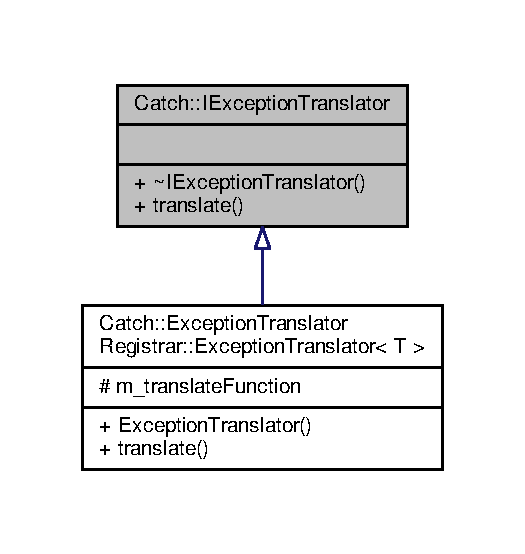
\includegraphics[width=252pt]{struct_catch_1_1_i_exception_translator__inherit__graph}
\end{center}
\end{figure}


Collaboration diagram for Catch\-:\-:I\-Exception\-Translator\-:
\nopagebreak
\begin{figure}[H]
\begin{center}
\leavevmode
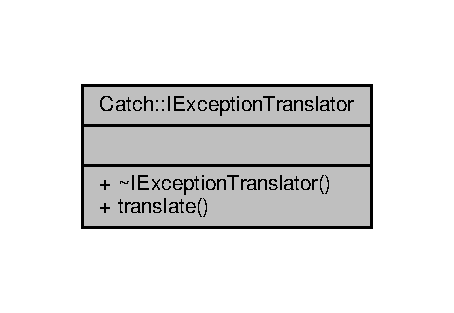
\includegraphics[width=218pt]{struct_catch_1_1_i_exception_translator__coll__graph}
\end{center}
\end{figure}
\subsection*{Public Member Functions}
\begin{DoxyCompactItemize}
\item 
virtual \hyperlink{struct_catch_1_1_i_exception_translator_afa00bb6258c07591df472aadae05783f}{$\sim$\-I\-Exception\-Translator} ()
\item 
virtual std\-::string \hyperlink{struct_catch_1_1_i_exception_translator_a2a554b96ed5ed411e7c796b6b42837a5}{translate} (Exception\-Translators\-::const\-\_\-iterator it, Exception\-Translators\-::const\-\_\-iterator it\-End) const =0
\end{DoxyCompactItemize}


\subsection{Constructor \& Destructor Documentation}
\hypertarget{struct_catch_1_1_i_exception_translator_afa00bb6258c07591df472aadae05783f}{\index{Catch\-::\-I\-Exception\-Translator@{Catch\-::\-I\-Exception\-Translator}!$\sim$\-I\-Exception\-Translator@{$\sim$\-I\-Exception\-Translator}}
\index{$\sim$\-I\-Exception\-Translator@{$\sim$\-I\-Exception\-Translator}!Catch::IExceptionTranslator@{Catch\-::\-I\-Exception\-Translator}}
\subsubsection[{$\sim$\-I\-Exception\-Translator}]{\setlength{\rightskip}{0pt plus 5cm}virtual Catch\-::\-I\-Exception\-Translator\-::$\sim$\-I\-Exception\-Translator (
\begin{DoxyParamCaption}
{}
\end{DoxyParamCaption}
)\hspace{0.3cm}{\ttfamily [virtual]}}}\label{struct_catch_1_1_i_exception_translator_afa00bb6258c07591df472aadae05783f}


\subsection{Member Function Documentation}
\hypertarget{struct_catch_1_1_i_exception_translator_a2a554b96ed5ed411e7c796b6b42837a5}{\index{Catch\-::\-I\-Exception\-Translator@{Catch\-::\-I\-Exception\-Translator}!translate@{translate}}
\index{translate@{translate}!Catch::IExceptionTranslator@{Catch\-::\-I\-Exception\-Translator}}
\subsubsection[{translate}]{\setlength{\rightskip}{0pt plus 5cm}virtual std\-::string Catch\-::\-I\-Exception\-Translator\-::translate (
\begin{DoxyParamCaption}
\item[{Exception\-Translators\-::const\-\_\-iterator}]{it, }
\item[{Exception\-Translators\-::const\-\_\-iterator}]{it\-End}
\end{DoxyParamCaption}
) const\hspace{0.3cm}{\ttfamily [pure virtual]}}}\label{struct_catch_1_1_i_exception_translator_a2a554b96ed5ed411e7c796b6b42837a5}


Implemented in \hyperlink{class_catch_1_1_exception_translator_registrar_1_1_exception_translator_a29e85940ee9ce719f26e43550cb4ed48}{Catch\-::\-Exception\-Translator\-Registrar\-::\-Exception\-Translator$<$ T $>$}.



The documentation for this struct was generated from the following file\-:\begin{DoxyCompactItemize}
\item 
\hyperlink{catch_8hpp}{catch.\-hpp}\end{DoxyCompactItemize}

\hypertarget{struct_catch_1_1_i_exception_translator_registry}{\section{Catch\-:\-:I\-Exception\-Translator\-Registry Struct Reference}
\label{struct_catch_1_1_i_exception_translator_registry}\index{Catch\-::\-I\-Exception\-Translator\-Registry@{Catch\-::\-I\-Exception\-Translator\-Registry}}
}


{\ttfamily \#include $<$catch.\-hpp$>$}



Collaboration diagram for Catch\-:\-:I\-Exception\-Translator\-Registry\-:
\nopagebreak
\begin{figure}[H]
\begin{center}
\leavevmode
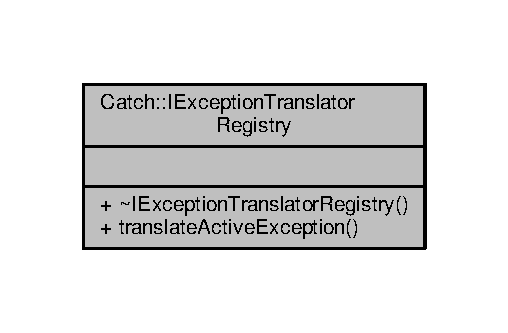
\includegraphics[width=244pt]{struct_catch_1_1_i_exception_translator_registry__coll__graph}
\end{center}
\end{figure}
\subsection*{Public Member Functions}
\begin{DoxyCompactItemize}
\item 
virtual \hyperlink{struct_catch_1_1_i_exception_translator_registry_acf7402e18789ea46d54ea8564ac358d3}{$\sim$\-I\-Exception\-Translator\-Registry} ()
\item 
virtual std\-::string \hyperlink{struct_catch_1_1_i_exception_translator_registry_af76ae8c331a17f2a94c9720bc0d686bb}{translate\-Active\-Exception} () const =0
\end{DoxyCompactItemize}


\subsection{Constructor \& Destructor Documentation}
\hypertarget{struct_catch_1_1_i_exception_translator_registry_acf7402e18789ea46d54ea8564ac358d3}{\index{Catch\-::\-I\-Exception\-Translator\-Registry@{Catch\-::\-I\-Exception\-Translator\-Registry}!$\sim$\-I\-Exception\-Translator\-Registry@{$\sim$\-I\-Exception\-Translator\-Registry}}
\index{$\sim$\-I\-Exception\-Translator\-Registry@{$\sim$\-I\-Exception\-Translator\-Registry}!Catch::IExceptionTranslatorRegistry@{Catch\-::\-I\-Exception\-Translator\-Registry}}
\subsubsection[{$\sim$\-I\-Exception\-Translator\-Registry}]{\setlength{\rightskip}{0pt plus 5cm}virtual Catch\-::\-I\-Exception\-Translator\-Registry\-::$\sim$\-I\-Exception\-Translator\-Registry (
\begin{DoxyParamCaption}
{}
\end{DoxyParamCaption}
)\hspace{0.3cm}{\ttfamily [virtual]}}}\label{struct_catch_1_1_i_exception_translator_registry_acf7402e18789ea46d54ea8564ac358d3}


\subsection{Member Function Documentation}
\hypertarget{struct_catch_1_1_i_exception_translator_registry_af76ae8c331a17f2a94c9720bc0d686bb}{\index{Catch\-::\-I\-Exception\-Translator\-Registry@{Catch\-::\-I\-Exception\-Translator\-Registry}!translate\-Active\-Exception@{translate\-Active\-Exception}}
\index{translate\-Active\-Exception@{translate\-Active\-Exception}!Catch::IExceptionTranslatorRegistry@{Catch\-::\-I\-Exception\-Translator\-Registry}}
\subsubsection[{translate\-Active\-Exception}]{\setlength{\rightskip}{0pt plus 5cm}virtual std\-::string Catch\-::\-I\-Exception\-Translator\-Registry\-::translate\-Active\-Exception (
\begin{DoxyParamCaption}
{}
\end{DoxyParamCaption}
) const\hspace{0.3cm}{\ttfamily [pure virtual]}}}\label{struct_catch_1_1_i_exception_translator_registry_af76ae8c331a17f2a94c9720bc0d686bb}


The documentation for this struct was generated from the following file\-:\begin{DoxyCompactItemize}
\item 
\hyperlink{catch_8hpp}{catch.\-hpp}\end{DoxyCompactItemize}

\hypertarget{struct_catch_1_1_i_mutable_registry_hub}{\section{Catch\-:\-:I\-Mutable\-Registry\-Hub Struct Reference}
\label{struct_catch_1_1_i_mutable_registry_hub}\index{Catch\-::\-I\-Mutable\-Registry\-Hub@{Catch\-::\-I\-Mutable\-Registry\-Hub}}
}


{\ttfamily \#include $<$catch.\-hpp$>$}



Collaboration diagram for Catch\-:\-:I\-Mutable\-Registry\-Hub\-:
\nopagebreak
\begin{figure}[H]
\begin{center}
\leavevmode
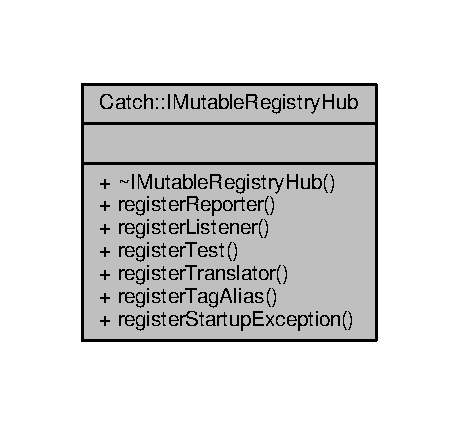
\includegraphics[width=220pt]{struct_catch_1_1_i_mutable_registry_hub__coll__graph}
\end{center}
\end{figure}
\subsection*{Public Member Functions}
\begin{DoxyCompactItemize}
\item 
virtual \hyperlink{struct_catch_1_1_i_mutable_registry_hub_a759ca1e044e19f905fb4d306f1367193}{$\sim$\-I\-Mutable\-Registry\-Hub} ()
\item 
virtual void \hyperlink{struct_catch_1_1_i_mutable_registry_hub_a1c0ac202ac31ee9f88e8ff5cbac4b243}{register\-Reporter} (std\-::string const \&name, \hyperlink{namespace_catch_ad1b36ac40c2739e52fd453dcdddf0d09}{I\-Reporter\-Factory\-Ptr} const \&factory)=0
\item 
virtual void \hyperlink{struct_catch_1_1_i_mutable_registry_hub_abd892a133f85581fd00ee75bb379ca56}{register\-Listener} (\hyperlink{namespace_catch_ad1b36ac40c2739e52fd453dcdddf0d09}{I\-Reporter\-Factory\-Ptr} const \&factory)=0
\item 
virtual void \hyperlink{struct_catch_1_1_i_mutable_registry_hub_a11b85c6744d88c9f83fe16ad4a8dd451}{register\-Test} (\hyperlink{class_catch_1_1_test_case}{Test\-Case} const \&test\-Info)=0
\item 
virtual void \hyperlink{struct_catch_1_1_i_mutable_registry_hub_ae6825365102693cf7707db022a2c2b49}{register\-Translator} (const \hyperlink{struct_catch_1_1_i_exception_translator}{I\-Exception\-Translator} $\ast$translator)=0
\item 
virtual void \hyperlink{struct_catch_1_1_i_mutable_registry_hub_abf2e386b6f94f615719ada711adbf822}{register\-Tag\-Alias} (std\-::string const \&alias, std\-::string const \&tag, \hyperlink{struct_catch_1_1_source_line_info}{Source\-Line\-Info} const \&line\-Info)=0
\item 
virtual void \hyperlink{struct_catch_1_1_i_mutable_registry_hub_a72a7d5386851ac3200f8da794a009c86}{register\-Startup\-Exception} () noexcept=0
\end{DoxyCompactItemize}


\subsection{Constructor \& Destructor Documentation}
\hypertarget{struct_catch_1_1_i_mutable_registry_hub_a759ca1e044e19f905fb4d306f1367193}{\index{Catch\-::\-I\-Mutable\-Registry\-Hub@{Catch\-::\-I\-Mutable\-Registry\-Hub}!$\sim$\-I\-Mutable\-Registry\-Hub@{$\sim$\-I\-Mutable\-Registry\-Hub}}
\index{$\sim$\-I\-Mutable\-Registry\-Hub@{$\sim$\-I\-Mutable\-Registry\-Hub}!Catch::IMutableRegistryHub@{Catch\-::\-I\-Mutable\-Registry\-Hub}}
\subsubsection[{$\sim$\-I\-Mutable\-Registry\-Hub}]{\setlength{\rightskip}{0pt plus 5cm}virtual Catch\-::\-I\-Mutable\-Registry\-Hub\-::$\sim$\-I\-Mutable\-Registry\-Hub (
\begin{DoxyParamCaption}
{}
\end{DoxyParamCaption}
)\hspace{0.3cm}{\ttfamily [virtual]}}}\label{struct_catch_1_1_i_mutable_registry_hub_a759ca1e044e19f905fb4d306f1367193}


\subsection{Member Function Documentation}
\hypertarget{struct_catch_1_1_i_mutable_registry_hub_abd892a133f85581fd00ee75bb379ca56}{\index{Catch\-::\-I\-Mutable\-Registry\-Hub@{Catch\-::\-I\-Mutable\-Registry\-Hub}!register\-Listener@{register\-Listener}}
\index{register\-Listener@{register\-Listener}!Catch::IMutableRegistryHub@{Catch\-::\-I\-Mutable\-Registry\-Hub}}
\subsubsection[{register\-Listener}]{\setlength{\rightskip}{0pt plus 5cm}virtual void Catch\-::\-I\-Mutable\-Registry\-Hub\-::register\-Listener (
\begin{DoxyParamCaption}
\item[{{\bf I\-Reporter\-Factory\-Ptr} const \&}]{factory}
\end{DoxyParamCaption}
)\hspace{0.3cm}{\ttfamily [pure virtual]}}}\label{struct_catch_1_1_i_mutable_registry_hub_abd892a133f85581fd00ee75bb379ca56}
\hypertarget{struct_catch_1_1_i_mutable_registry_hub_a1c0ac202ac31ee9f88e8ff5cbac4b243}{\index{Catch\-::\-I\-Mutable\-Registry\-Hub@{Catch\-::\-I\-Mutable\-Registry\-Hub}!register\-Reporter@{register\-Reporter}}
\index{register\-Reporter@{register\-Reporter}!Catch::IMutableRegistryHub@{Catch\-::\-I\-Mutable\-Registry\-Hub}}
\subsubsection[{register\-Reporter}]{\setlength{\rightskip}{0pt plus 5cm}virtual void Catch\-::\-I\-Mutable\-Registry\-Hub\-::register\-Reporter (
\begin{DoxyParamCaption}
\item[{std\-::string const \&}]{name, }
\item[{{\bf I\-Reporter\-Factory\-Ptr} const \&}]{factory}
\end{DoxyParamCaption}
)\hspace{0.3cm}{\ttfamily [pure virtual]}}}\label{struct_catch_1_1_i_mutable_registry_hub_a1c0ac202ac31ee9f88e8ff5cbac4b243}
\hypertarget{struct_catch_1_1_i_mutable_registry_hub_a72a7d5386851ac3200f8da794a009c86}{\index{Catch\-::\-I\-Mutable\-Registry\-Hub@{Catch\-::\-I\-Mutable\-Registry\-Hub}!register\-Startup\-Exception@{register\-Startup\-Exception}}
\index{register\-Startup\-Exception@{register\-Startup\-Exception}!Catch::IMutableRegistryHub@{Catch\-::\-I\-Mutable\-Registry\-Hub}}
\subsubsection[{register\-Startup\-Exception}]{\setlength{\rightskip}{0pt plus 5cm}virtual void Catch\-::\-I\-Mutable\-Registry\-Hub\-::register\-Startup\-Exception (
\begin{DoxyParamCaption}
{}
\end{DoxyParamCaption}
)\hspace{0.3cm}{\ttfamily [pure virtual]}, {\ttfamily [noexcept]}}}\label{struct_catch_1_1_i_mutable_registry_hub_a72a7d5386851ac3200f8da794a009c86}
\hypertarget{struct_catch_1_1_i_mutable_registry_hub_abf2e386b6f94f615719ada711adbf822}{\index{Catch\-::\-I\-Mutable\-Registry\-Hub@{Catch\-::\-I\-Mutable\-Registry\-Hub}!register\-Tag\-Alias@{register\-Tag\-Alias}}
\index{register\-Tag\-Alias@{register\-Tag\-Alias}!Catch::IMutableRegistryHub@{Catch\-::\-I\-Mutable\-Registry\-Hub}}
\subsubsection[{register\-Tag\-Alias}]{\setlength{\rightskip}{0pt plus 5cm}virtual void Catch\-::\-I\-Mutable\-Registry\-Hub\-::register\-Tag\-Alias (
\begin{DoxyParamCaption}
\item[{std\-::string const \&}]{alias, }
\item[{std\-::string const \&}]{tag, }
\item[{{\bf Source\-Line\-Info} const \&}]{line\-Info}
\end{DoxyParamCaption}
)\hspace{0.3cm}{\ttfamily [pure virtual]}}}\label{struct_catch_1_1_i_mutable_registry_hub_abf2e386b6f94f615719ada711adbf822}
\hypertarget{struct_catch_1_1_i_mutable_registry_hub_a11b85c6744d88c9f83fe16ad4a8dd451}{\index{Catch\-::\-I\-Mutable\-Registry\-Hub@{Catch\-::\-I\-Mutable\-Registry\-Hub}!register\-Test@{register\-Test}}
\index{register\-Test@{register\-Test}!Catch::IMutableRegistryHub@{Catch\-::\-I\-Mutable\-Registry\-Hub}}
\subsubsection[{register\-Test}]{\setlength{\rightskip}{0pt plus 5cm}virtual void Catch\-::\-I\-Mutable\-Registry\-Hub\-::register\-Test (
\begin{DoxyParamCaption}
\item[{{\bf Test\-Case} const \&}]{test\-Info}
\end{DoxyParamCaption}
)\hspace{0.3cm}{\ttfamily [pure virtual]}}}\label{struct_catch_1_1_i_mutable_registry_hub_a11b85c6744d88c9f83fe16ad4a8dd451}
\hypertarget{struct_catch_1_1_i_mutable_registry_hub_ae6825365102693cf7707db022a2c2b49}{\index{Catch\-::\-I\-Mutable\-Registry\-Hub@{Catch\-::\-I\-Mutable\-Registry\-Hub}!register\-Translator@{register\-Translator}}
\index{register\-Translator@{register\-Translator}!Catch::IMutableRegistryHub@{Catch\-::\-I\-Mutable\-Registry\-Hub}}
\subsubsection[{register\-Translator}]{\setlength{\rightskip}{0pt plus 5cm}virtual void Catch\-::\-I\-Mutable\-Registry\-Hub\-::register\-Translator (
\begin{DoxyParamCaption}
\item[{const {\bf I\-Exception\-Translator} $\ast$}]{translator}
\end{DoxyParamCaption}
)\hspace{0.3cm}{\ttfamily [pure virtual]}}}\label{struct_catch_1_1_i_mutable_registry_hub_ae6825365102693cf7707db022a2c2b49}


Referenced by Catch\-::\-Exception\-Translator\-Registrar\-::\-Exception\-Translator\-Registrar().



The documentation for this struct was generated from the following file\-:\begin{DoxyCompactItemize}
\item 
\hyperlink{catch_8hpp}{catch.\-hpp}\end{DoxyCompactItemize}

\hypertarget{class_input_receiver}{}\section{Input\+Receiver Class Reference}
\label{class_input_receiver}\index{Input\+Receiver@{Input\+Receiver}}
Inheritance diagram for Input\+Receiver\+:\begin{figure}[H]
\begin{center}
\leavevmode
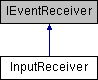
\includegraphics[height=2.000000cm]{class_input_receiver}
\end{center}
\end{figure}
\subsection*{Public Member Functions}
\begin{DoxyCompactItemize}
\item 
\mbox{\Hypertarget{class_input_receiver_a93d0cb79217595eb9bc29f5785bb5620}\label{class_input_receiver_a93d0cb79217595eb9bc29f5785bb5620}} 
irr\+::core\+::array$<$ irr\+::\+S\+Joystick\+Info $>$ {\bfseries Get\+Joystick\+Info} ()
\item 
\mbox{\Hypertarget{class_input_receiver_a0f4ecd33eace7fe2778cba699a06cd82}\label{class_input_receiver_a0f4ecd33eace7fe2778cba699a06cd82}} 
void {\bfseries Check\+Joystick\+Present} (irr\+::\+Irrlicht\+Device $\ast$device)
\item 
\mbox{\Hypertarget{class_input_receiver_a8cbad01c0e0dcaa953685b1c932d8ce6}\label{class_input_receiver_a8cbad01c0e0dcaa953685b1c932d8ce6}} 
bool {\bfseries On\+Event} (const irr\+::\+S\+Event \&event)
\item 
\mbox{\Hypertarget{class_input_receiver_a736d040738e9826b2abbcc0dd9cd085c}\label{class_input_receiver_a736d040738e9826b2abbcc0dd9cd085c}} 
bool {\bfseries Is\+Key\+Down} (irr\+::\+E\+K\+E\+Y\+\_\+\+C\+O\+DE key\+Code) const
\end{DoxyCompactItemize}
\subsection*{Static Public Attributes}
\begin{DoxyCompactItemize}
\item 
\mbox{\Hypertarget{class_input_receiver_a1763dd9cc9a31639592fb23115cdcc64}\label{class_input_receiver_a1763dd9cc9a31639592fb23115cdcc64}} 
static bool {\bfseries is\+Left\+Mouse\+Button\+Down} = false
\item 
\mbox{\Hypertarget{class_input_receiver_a4bffdbd7b8b83008a8f0d79ab018bb6b}\label{class_input_receiver_a4bffdbd7b8b83008a8f0d79ab018bb6b}} 
static irr\+::core\+::vector3df {\bfseries position} = core\+::vector3df(0,0,0)
\item 
\mbox{\Hypertarget{class_input_receiver_ad5486727fcb5faf69809b69f311c0b27}\label{class_input_receiver_ad5486727fcb5faf69809b69f311c0b27}} 
static irr\+::\+S\+Event\+::\+S\+Joystick\+Event {\bfseries joystick\+State}
\end{DoxyCompactItemize}
\subsection*{Private Attributes}
\begin{DoxyCompactItemize}
\item 
\mbox{\Hypertarget{class_input_receiver_a86ce1bb3b52f6bb3499224a508178f10}\label{class_input_receiver_a86ce1bb3b52f6bb3499224a508178f10}} 
bool {\bfseries key\+Is\+Down} \mbox{[}irr\+::\+K\+E\+Y\+\_\+\+K\+E\+Y\+\_\+\+C\+O\+D\+E\+S\+\_\+\+C\+O\+U\+NT\mbox{]}
\item 
\mbox{\Hypertarget{class_input_receiver_ab201d50024317b870b7020843033fd4a}\label{class_input_receiver_ab201d50024317b870b7020843033fd4a}} 
irr\+::core\+::array$<$ irr\+::\+S\+Joystick\+Info $>$ {\bfseries joystick\+Info}
\end{DoxyCompactItemize}


The documentation for this class was generated from the following files\+:\begin{DoxyCompactItemize}
\item 
D\+:/\+Documenten/\+S\+T\+U\+D\+I\+E G\+D/\+Game Engine/\+Irrlicht project/kommandos/Input\+Receiver.\+h\item 
D\+:/\+Documenten/\+S\+T\+U\+D\+I\+E G\+D/\+Game Engine/\+Irrlicht project/kommandos/Input\+Receiver.\+cpp\end{DoxyCompactItemize}

\hypertarget{struct_catch_1_1_i_registry_hub}{\section{Catch\-:\-:I\-Registry\-Hub Struct Reference}
\label{struct_catch_1_1_i_registry_hub}\index{Catch\-::\-I\-Registry\-Hub@{Catch\-::\-I\-Registry\-Hub}}
}


{\ttfamily \#include $<$catch.\-hpp$>$}



Collaboration diagram for Catch\-:\-:I\-Registry\-Hub\-:
\nopagebreak
\begin{figure}[H]
\begin{center}
\leavevmode
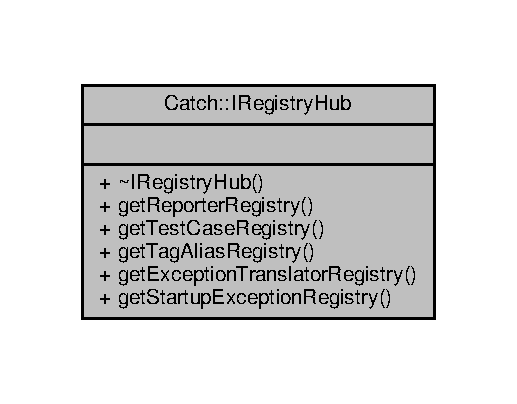
\includegraphics[width=248pt]{struct_catch_1_1_i_registry_hub__coll__graph}
\end{center}
\end{figure}
\subsection*{Public Member Functions}
\begin{DoxyCompactItemize}
\item 
virtual \hyperlink{struct_catch_1_1_i_registry_hub_a050de0f27f96888c8b410992146c9a09}{$\sim$\-I\-Registry\-Hub} ()
\item 
virtual I\-Reporter\-Registry const \& \hyperlink{struct_catch_1_1_i_registry_hub_a55534563f7ecf7e20ec1e37285ebe54d}{get\-Reporter\-Registry} () const =0
\item 
virtual \hyperlink{struct_catch_1_1_i_test_case_registry}{I\-Test\-Case\-Registry} const \& \hyperlink{struct_catch_1_1_i_registry_hub_af4f6255f0c0f8f1f179fa9d7d4843076}{get\-Test\-Case\-Registry} () const =0
\item 
virtual I\-Tag\-Alias\-Registry const \& \hyperlink{struct_catch_1_1_i_registry_hub_a3c511b1d33e5a6d95c333a0ff387df1a}{get\-Tag\-Alias\-Registry} () const =0
\item 
virtual \\*
\hyperlink{struct_catch_1_1_i_exception_translator_registry}{I\-Exception\-Translator\-Registry} \& \hyperlink{struct_catch_1_1_i_registry_hub_a3606988da110c016c5af3ae63454eb78}{get\-Exception\-Translator\-Registry} ()=0
\item 
virtual \\*
Startup\-Exception\-Registry const \& \hyperlink{struct_catch_1_1_i_registry_hub_a00281210628e6c616aca1d3e0d84db04}{get\-Startup\-Exception\-Registry} () const =0
\end{DoxyCompactItemize}


\subsection{Constructor \& Destructor Documentation}
\hypertarget{struct_catch_1_1_i_registry_hub_a050de0f27f96888c8b410992146c9a09}{\index{Catch\-::\-I\-Registry\-Hub@{Catch\-::\-I\-Registry\-Hub}!$\sim$\-I\-Registry\-Hub@{$\sim$\-I\-Registry\-Hub}}
\index{$\sim$\-I\-Registry\-Hub@{$\sim$\-I\-Registry\-Hub}!Catch::IRegistryHub@{Catch\-::\-I\-Registry\-Hub}}
\subsubsection[{$\sim$\-I\-Registry\-Hub}]{\setlength{\rightskip}{0pt plus 5cm}virtual Catch\-::\-I\-Registry\-Hub\-::$\sim$\-I\-Registry\-Hub (
\begin{DoxyParamCaption}
{}
\end{DoxyParamCaption}
)\hspace{0.3cm}{\ttfamily [virtual]}}}\label{struct_catch_1_1_i_registry_hub_a050de0f27f96888c8b410992146c9a09}


\subsection{Member Function Documentation}
\hypertarget{struct_catch_1_1_i_registry_hub_a3606988da110c016c5af3ae63454eb78}{\index{Catch\-::\-I\-Registry\-Hub@{Catch\-::\-I\-Registry\-Hub}!get\-Exception\-Translator\-Registry@{get\-Exception\-Translator\-Registry}}
\index{get\-Exception\-Translator\-Registry@{get\-Exception\-Translator\-Registry}!Catch::IRegistryHub@{Catch\-::\-I\-Registry\-Hub}}
\subsubsection[{get\-Exception\-Translator\-Registry}]{\setlength{\rightskip}{0pt plus 5cm}virtual {\bf I\-Exception\-Translator\-Registry}\& Catch\-::\-I\-Registry\-Hub\-::get\-Exception\-Translator\-Registry (
\begin{DoxyParamCaption}
{}
\end{DoxyParamCaption}
)\hspace{0.3cm}{\ttfamily [pure virtual]}}}\label{struct_catch_1_1_i_registry_hub_a3606988da110c016c5af3ae63454eb78}
\hypertarget{struct_catch_1_1_i_registry_hub_a55534563f7ecf7e20ec1e37285ebe54d}{\index{Catch\-::\-I\-Registry\-Hub@{Catch\-::\-I\-Registry\-Hub}!get\-Reporter\-Registry@{get\-Reporter\-Registry}}
\index{get\-Reporter\-Registry@{get\-Reporter\-Registry}!Catch::IRegistryHub@{Catch\-::\-I\-Registry\-Hub}}
\subsubsection[{get\-Reporter\-Registry}]{\setlength{\rightskip}{0pt plus 5cm}virtual I\-Reporter\-Registry const\& Catch\-::\-I\-Registry\-Hub\-::get\-Reporter\-Registry (
\begin{DoxyParamCaption}
{}
\end{DoxyParamCaption}
) const\hspace{0.3cm}{\ttfamily [pure virtual]}}}\label{struct_catch_1_1_i_registry_hub_a55534563f7ecf7e20ec1e37285ebe54d}
\hypertarget{struct_catch_1_1_i_registry_hub_a00281210628e6c616aca1d3e0d84db04}{\index{Catch\-::\-I\-Registry\-Hub@{Catch\-::\-I\-Registry\-Hub}!get\-Startup\-Exception\-Registry@{get\-Startup\-Exception\-Registry}}
\index{get\-Startup\-Exception\-Registry@{get\-Startup\-Exception\-Registry}!Catch::IRegistryHub@{Catch\-::\-I\-Registry\-Hub}}
\subsubsection[{get\-Startup\-Exception\-Registry}]{\setlength{\rightskip}{0pt plus 5cm}virtual Startup\-Exception\-Registry const\& Catch\-::\-I\-Registry\-Hub\-::get\-Startup\-Exception\-Registry (
\begin{DoxyParamCaption}
{}
\end{DoxyParamCaption}
) const\hspace{0.3cm}{\ttfamily [pure virtual]}}}\label{struct_catch_1_1_i_registry_hub_a00281210628e6c616aca1d3e0d84db04}
\hypertarget{struct_catch_1_1_i_registry_hub_a3c511b1d33e5a6d95c333a0ff387df1a}{\index{Catch\-::\-I\-Registry\-Hub@{Catch\-::\-I\-Registry\-Hub}!get\-Tag\-Alias\-Registry@{get\-Tag\-Alias\-Registry}}
\index{get\-Tag\-Alias\-Registry@{get\-Tag\-Alias\-Registry}!Catch::IRegistryHub@{Catch\-::\-I\-Registry\-Hub}}
\subsubsection[{get\-Tag\-Alias\-Registry}]{\setlength{\rightskip}{0pt plus 5cm}virtual I\-Tag\-Alias\-Registry const\& Catch\-::\-I\-Registry\-Hub\-::get\-Tag\-Alias\-Registry (
\begin{DoxyParamCaption}
{}
\end{DoxyParamCaption}
) const\hspace{0.3cm}{\ttfamily [pure virtual]}}}\label{struct_catch_1_1_i_registry_hub_a3c511b1d33e5a6d95c333a0ff387df1a}
\hypertarget{struct_catch_1_1_i_registry_hub_af4f6255f0c0f8f1f179fa9d7d4843076}{\index{Catch\-::\-I\-Registry\-Hub@{Catch\-::\-I\-Registry\-Hub}!get\-Test\-Case\-Registry@{get\-Test\-Case\-Registry}}
\index{get\-Test\-Case\-Registry@{get\-Test\-Case\-Registry}!Catch::IRegistryHub@{Catch\-::\-I\-Registry\-Hub}}
\subsubsection[{get\-Test\-Case\-Registry}]{\setlength{\rightskip}{0pt plus 5cm}virtual {\bf I\-Test\-Case\-Registry} const\& Catch\-::\-I\-Registry\-Hub\-::get\-Test\-Case\-Registry (
\begin{DoxyParamCaption}
{}
\end{DoxyParamCaption}
) const\hspace{0.3cm}{\ttfamily [pure virtual]}}}\label{struct_catch_1_1_i_registry_hub_af4f6255f0c0f8f1f179fa9d7d4843076}


The documentation for this struct was generated from the following file\-:\begin{DoxyCompactItemize}
\item 
\hyperlink{catch_8hpp}{catch.\-hpp}\end{DoxyCompactItemize}

\hypertarget{struct_catch_1_1_i_result_capture}{\section{Catch\-:\-:I\-Result\-Capture Struct Reference}
\label{struct_catch_1_1_i_result_capture}\index{Catch\-::\-I\-Result\-Capture@{Catch\-::\-I\-Result\-Capture}}
}


{\ttfamily \#include $<$catch.\-hpp$>$}



Collaboration diagram for Catch\-:\-:I\-Result\-Capture\-:
\nopagebreak
\begin{figure}[H]
\begin{center}
\leavevmode
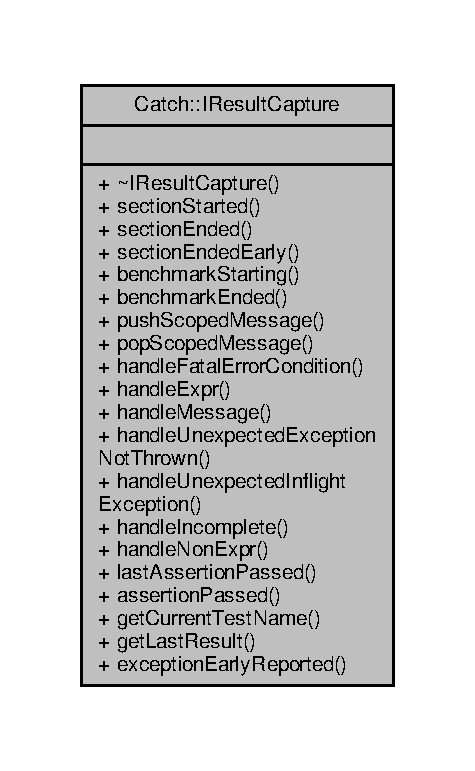
\includegraphics[width=228pt]{struct_catch_1_1_i_result_capture__coll__graph}
\end{center}
\end{figure}
\subsection*{Public Member Functions}
\begin{DoxyCompactItemize}
\item 
virtual \hyperlink{struct_catch_1_1_i_result_capture_a3bd16719d6772b7470887fc36c6d0808}{$\sim$\-I\-Result\-Capture} ()
\item 
virtual bool \hyperlink{struct_catch_1_1_i_result_capture_a5b76ed52badcb64cf374202e12b81a03}{section\-Started} (\hyperlink{struct_catch_1_1_section_info}{Section\-Info} const \&section\-Info, \hyperlink{struct_catch_1_1_counts}{Counts} \&assertions)=0
\item 
virtual void \hyperlink{struct_catch_1_1_i_result_capture_a4e152bc43dc0933684e31fa67a58195d}{section\-Ended} (\hyperlink{struct_catch_1_1_section_end_info}{Section\-End\-Info} const \&end\-Info)=0
\item 
virtual void \hyperlink{struct_catch_1_1_i_result_capture_afcc71eef8ca821ae132cced4a2be6988}{section\-Ended\-Early} (\hyperlink{struct_catch_1_1_section_end_info}{Section\-End\-Info} const \&end\-Info)=0
\item 
virtual void \hyperlink{struct_catch_1_1_i_result_capture_a264ae12330c74b2daae41715a30d51bf}{benchmark\-Starting} (Benchmark\-Info const \&info)=0
\item 
virtual void \hyperlink{struct_catch_1_1_i_result_capture_a6e5e64f9d94211a888249012ab6cc7fb}{benchmark\-Ended} (Benchmark\-Stats const \&stats)=0
\item 
virtual void \hyperlink{struct_catch_1_1_i_result_capture_a91d154c1e087e383dcde5aad95cb6a05}{push\-Scoped\-Message} (\hyperlink{struct_catch_1_1_message_info}{Message\-Info} const \&message)=0
\item 
virtual void \hyperlink{struct_catch_1_1_i_result_capture_a42bcb13276706bf8c3ce081ce16d37fd}{pop\-Scoped\-Message} (\hyperlink{struct_catch_1_1_message_info}{Message\-Info} const \&message)=0
\item 
virtual void \hyperlink{struct_catch_1_1_i_result_capture_a48559e6598ba9474b903697b69c769b2}{handle\-Fatal\-Error\-Condition} (\hyperlink{class_catch_1_1_string_ref}{String\-Ref} message)=0
\item 
virtual void \hyperlink{struct_catch_1_1_i_result_capture_a59a2b05391e464954575d2afb6d5d607}{handle\-Expr} (\hyperlink{struct_catch_1_1_assertion_info}{Assertion\-Info} const \&info, \hyperlink{struct_catch_1_1_i_transient_expression}{I\-Transient\-Expression} const \&expr, \hyperlink{struct_catch_1_1_assertion_reaction}{Assertion\-Reaction} \&reaction)=0
\item 
virtual void \hyperlink{struct_catch_1_1_i_result_capture_a21788ebc64571abf322b80c8cc51794d}{handle\-Message} (\hyperlink{struct_catch_1_1_assertion_info}{Assertion\-Info} const \&info, \hyperlink{struct_catch_1_1_result_was_a624e1ee3661fcf6094ceef1f654601ef}{Result\-Was\-::\-Of\-Type} result\-Type, \hyperlink{class_catch_1_1_string_ref}{String\-Ref} const \&message, \hyperlink{struct_catch_1_1_assertion_reaction}{Assertion\-Reaction} \&reaction)=0
\item 
virtual void \hyperlink{struct_catch_1_1_i_result_capture_a6382ed20486e2d9a020da971c6d5c53d}{handle\-Unexpected\-Exception\-Not\-Thrown} (\hyperlink{struct_catch_1_1_assertion_info}{Assertion\-Info} const \&info, \hyperlink{struct_catch_1_1_assertion_reaction}{Assertion\-Reaction} \&reaction)=0
\item 
virtual void \hyperlink{struct_catch_1_1_i_result_capture_afc97bc69829185222f955ebeef97adfe}{handle\-Unexpected\-Inflight\-Exception} (\hyperlink{struct_catch_1_1_assertion_info}{Assertion\-Info} const \&info, std\-::string const \&message, \hyperlink{struct_catch_1_1_assertion_reaction}{Assertion\-Reaction} \&reaction)=0
\item 
virtual void \hyperlink{struct_catch_1_1_i_result_capture_a89b89372eb09cc44f8dcad363de6157d}{handle\-Incomplete} (\hyperlink{struct_catch_1_1_assertion_info}{Assertion\-Info} const \&info)=0
\item 
virtual void \hyperlink{struct_catch_1_1_i_result_capture_ab7dbdf8aa28427119583e24dbb302c63}{handle\-Non\-Expr} (\hyperlink{struct_catch_1_1_assertion_info}{Assertion\-Info} const \&info, \hyperlink{struct_catch_1_1_result_was_a624e1ee3661fcf6094ceef1f654601ef}{Result\-Was\-::\-Of\-Type} result\-Type, \hyperlink{struct_catch_1_1_assertion_reaction}{Assertion\-Reaction} \&reaction)=0
\item 
virtual bool \hyperlink{struct_catch_1_1_i_result_capture_a973435fbdcb2f6f07a0ec5719a01e956}{last\-Assertion\-Passed} ()=0
\item 
virtual void \hyperlink{struct_catch_1_1_i_result_capture_a9b0ef2cb071e9a9dc6ec1b533026aea7}{assertion\-Passed} ()=0
\item 
virtual std\-::string \hyperlink{struct_catch_1_1_i_result_capture_aea1617f4a84cc648246aa3ed6918b5bf}{get\-Current\-Test\-Name} () const =0
\item 
virtual const Assertion\-Result $\ast$ \hyperlink{struct_catch_1_1_i_result_capture_ab18872c89fab97405a56e9c6a4919736}{get\-Last\-Result} () const =0
\item 
virtual void \hyperlink{struct_catch_1_1_i_result_capture_ae63ecec95db4c236c63ecf616f483810}{exception\-Early\-Reported} ()=0
\end{DoxyCompactItemize}


\subsection{Constructor \& Destructor Documentation}
\hypertarget{struct_catch_1_1_i_result_capture_a3bd16719d6772b7470887fc36c6d0808}{\index{Catch\-::\-I\-Result\-Capture@{Catch\-::\-I\-Result\-Capture}!$\sim$\-I\-Result\-Capture@{$\sim$\-I\-Result\-Capture}}
\index{$\sim$\-I\-Result\-Capture@{$\sim$\-I\-Result\-Capture}!Catch::IResultCapture@{Catch\-::\-I\-Result\-Capture}}
\subsubsection[{$\sim$\-I\-Result\-Capture}]{\setlength{\rightskip}{0pt plus 5cm}virtual Catch\-::\-I\-Result\-Capture\-::$\sim$\-I\-Result\-Capture (
\begin{DoxyParamCaption}
{}
\end{DoxyParamCaption}
)\hspace{0.3cm}{\ttfamily [virtual]}}}\label{struct_catch_1_1_i_result_capture_a3bd16719d6772b7470887fc36c6d0808}


\subsection{Member Function Documentation}
\hypertarget{struct_catch_1_1_i_result_capture_a9b0ef2cb071e9a9dc6ec1b533026aea7}{\index{Catch\-::\-I\-Result\-Capture@{Catch\-::\-I\-Result\-Capture}!assertion\-Passed@{assertion\-Passed}}
\index{assertion\-Passed@{assertion\-Passed}!Catch::IResultCapture@{Catch\-::\-I\-Result\-Capture}}
\subsubsection[{assertion\-Passed}]{\setlength{\rightskip}{0pt plus 5cm}virtual void Catch\-::\-I\-Result\-Capture\-::assertion\-Passed (
\begin{DoxyParamCaption}
{}
\end{DoxyParamCaption}
)\hspace{0.3cm}{\ttfamily [pure virtual]}}}\label{struct_catch_1_1_i_result_capture_a9b0ef2cb071e9a9dc6ec1b533026aea7}
\hypertarget{struct_catch_1_1_i_result_capture_a6e5e64f9d94211a888249012ab6cc7fb}{\index{Catch\-::\-I\-Result\-Capture@{Catch\-::\-I\-Result\-Capture}!benchmark\-Ended@{benchmark\-Ended}}
\index{benchmark\-Ended@{benchmark\-Ended}!Catch::IResultCapture@{Catch\-::\-I\-Result\-Capture}}
\subsubsection[{benchmark\-Ended}]{\setlength{\rightskip}{0pt plus 5cm}virtual void Catch\-::\-I\-Result\-Capture\-::benchmark\-Ended (
\begin{DoxyParamCaption}
\item[{Benchmark\-Stats const \&}]{stats}
\end{DoxyParamCaption}
)\hspace{0.3cm}{\ttfamily [pure virtual]}}}\label{struct_catch_1_1_i_result_capture_a6e5e64f9d94211a888249012ab6cc7fb}
\hypertarget{struct_catch_1_1_i_result_capture_a264ae12330c74b2daae41715a30d51bf}{\index{Catch\-::\-I\-Result\-Capture@{Catch\-::\-I\-Result\-Capture}!benchmark\-Starting@{benchmark\-Starting}}
\index{benchmark\-Starting@{benchmark\-Starting}!Catch::IResultCapture@{Catch\-::\-I\-Result\-Capture}}
\subsubsection[{benchmark\-Starting}]{\setlength{\rightskip}{0pt plus 5cm}virtual void Catch\-::\-I\-Result\-Capture\-::benchmark\-Starting (
\begin{DoxyParamCaption}
\item[{Benchmark\-Info const \&}]{info}
\end{DoxyParamCaption}
)\hspace{0.3cm}{\ttfamily [pure virtual]}}}\label{struct_catch_1_1_i_result_capture_a264ae12330c74b2daae41715a30d51bf}
\hypertarget{struct_catch_1_1_i_result_capture_ae63ecec95db4c236c63ecf616f483810}{\index{Catch\-::\-I\-Result\-Capture@{Catch\-::\-I\-Result\-Capture}!exception\-Early\-Reported@{exception\-Early\-Reported}}
\index{exception\-Early\-Reported@{exception\-Early\-Reported}!Catch::IResultCapture@{Catch\-::\-I\-Result\-Capture}}
\subsubsection[{exception\-Early\-Reported}]{\setlength{\rightskip}{0pt plus 5cm}virtual void Catch\-::\-I\-Result\-Capture\-::exception\-Early\-Reported (
\begin{DoxyParamCaption}
{}
\end{DoxyParamCaption}
)\hspace{0.3cm}{\ttfamily [pure virtual]}}}\label{struct_catch_1_1_i_result_capture_ae63ecec95db4c236c63ecf616f483810}
\hypertarget{struct_catch_1_1_i_result_capture_aea1617f4a84cc648246aa3ed6918b5bf}{\index{Catch\-::\-I\-Result\-Capture@{Catch\-::\-I\-Result\-Capture}!get\-Current\-Test\-Name@{get\-Current\-Test\-Name}}
\index{get\-Current\-Test\-Name@{get\-Current\-Test\-Name}!Catch::IResultCapture@{Catch\-::\-I\-Result\-Capture}}
\subsubsection[{get\-Current\-Test\-Name}]{\setlength{\rightskip}{0pt plus 5cm}virtual std\-::string Catch\-::\-I\-Result\-Capture\-::get\-Current\-Test\-Name (
\begin{DoxyParamCaption}
{}
\end{DoxyParamCaption}
) const\hspace{0.3cm}{\ttfamily [pure virtual]}}}\label{struct_catch_1_1_i_result_capture_aea1617f4a84cc648246aa3ed6918b5bf}
\hypertarget{struct_catch_1_1_i_result_capture_ab18872c89fab97405a56e9c6a4919736}{\index{Catch\-::\-I\-Result\-Capture@{Catch\-::\-I\-Result\-Capture}!get\-Last\-Result@{get\-Last\-Result}}
\index{get\-Last\-Result@{get\-Last\-Result}!Catch::IResultCapture@{Catch\-::\-I\-Result\-Capture}}
\subsubsection[{get\-Last\-Result}]{\setlength{\rightskip}{0pt plus 5cm}virtual const Assertion\-Result$\ast$ Catch\-::\-I\-Result\-Capture\-::get\-Last\-Result (
\begin{DoxyParamCaption}
{}
\end{DoxyParamCaption}
) const\hspace{0.3cm}{\ttfamily [pure virtual]}}}\label{struct_catch_1_1_i_result_capture_ab18872c89fab97405a56e9c6a4919736}
\hypertarget{struct_catch_1_1_i_result_capture_a59a2b05391e464954575d2afb6d5d607}{\index{Catch\-::\-I\-Result\-Capture@{Catch\-::\-I\-Result\-Capture}!handle\-Expr@{handle\-Expr}}
\index{handle\-Expr@{handle\-Expr}!Catch::IResultCapture@{Catch\-::\-I\-Result\-Capture}}
\subsubsection[{handle\-Expr}]{\setlength{\rightskip}{0pt plus 5cm}virtual void Catch\-::\-I\-Result\-Capture\-::handle\-Expr (
\begin{DoxyParamCaption}
\item[{{\bf Assertion\-Info} const \&}]{info, }
\item[{{\bf I\-Transient\-Expression} const \&}]{expr, }
\item[{{\bf Assertion\-Reaction} \&}]{reaction}
\end{DoxyParamCaption}
)\hspace{0.3cm}{\ttfamily [pure virtual]}}}\label{struct_catch_1_1_i_result_capture_a59a2b05391e464954575d2afb6d5d607}
\hypertarget{struct_catch_1_1_i_result_capture_a48559e6598ba9474b903697b69c769b2}{\index{Catch\-::\-I\-Result\-Capture@{Catch\-::\-I\-Result\-Capture}!handle\-Fatal\-Error\-Condition@{handle\-Fatal\-Error\-Condition}}
\index{handle\-Fatal\-Error\-Condition@{handle\-Fatal\-Error\-Condition}!Catch::IResultCapture@{Catch\-::\-I\-Result\-Capture}}
\subsubsection[{handle\-Fatal\-Error\-Condition}]{\setlength{\rightskip}{0pt plus 5cm}virtual void Catch\-::\-I\-Result\-Capture\-::handle\-Fatal\-Error\-Condition (
\begin{DoxyParamCaption}
\item[{{\bf String\-Ref}}]{message}
\end{DoxyParamCaption}
)\hspace{0.3cm}{\ttfamily [pure virtual]}}}\label{struct_catch_1_1_i_result_capture_a48559e6598ba9474b903697b69c769b2}
\hypertarget{struct_catch_1_1_i_result_capture_a89b89372eb09cc44f8dcad363de6157d}{\index{Catch\-::\-I\-Result\-Capture@{Catch\-::\-I\-Result\-Capture}!handle\-Incomplete@{handle\-Incomplete}}
\index{handle\-Incomplete@{handle\-Incomplete}!Catch::IResultCapture@{Catch\-::\-I\-Result\-Capture}}
\subsubsection[{handle\-Incomplete}]{\setlength{\rightskip}{0pt plus 5cm}virtual void Catch\-::\-I\-Result\-Capture\-::handle\-Incomplete (
\begin{DoxyParamCaption}
\item[{{\bf Assertion\-Info} const \&}]{info}
\end{DoxyParamCaption}
)\hspace{0.3cm}{\ttfamily [pure virtual]}}}\label{struct_catch_1_1_i_result_capture_a89b89372eb09cc44f8dcad363de6157d}
\hypertarget{struct_catch_1_1_i_result_capture_a21788ebc64571abf322b80c8cc51794d}{\index{Catch\-::\-I\-Result\-Capture@{Catch\-::\-I\-Result\-Capture}!handle\-Message@{handle\-Message}}
\index{handle\-Message@{handle\-Message}!Catch::IResultCapture@{Catch\-::\-I\-Result\-Capture}}
\subsubsection[{handle\-Message}]{\setlength{\rightskip}{0pt plus 5cm}virtual void Catch\-::\-I\-Result\-Capture\-::handle\-Message (
\begin{DoxyParamCaption}
\item[{{\bf Assertion\-Info} const \&}]{info, }
\item[{{\bf Result\-Was\-::\-Of\-Type}}]{result\-Type, }
\item[{{\bf String\-Ref} const \&}]{message, }
\item[{{\bf Assertion\-Reaction} \&}]{reaction}
\end{DoxyParamCaption}
)\hspace{0.3cm}{\ttfamily [pure virtual]}}}\label{struct_catch_1_1_i_result_capture_a21788ebc64571abf322b80c8cc51794d}
\hypertarget{struct_catch_1_1_i_result_capture_ab7dbdf8aa28427119583e24dbb302c63}{\index{Catch\-::\-I\-Result\-Capture@{Catch\-::\-I\-Result\-Capture}!handle\-Non\-Expr@{handle\-Non\-Expr}}
\index{handle\-Non\-Expr@{handle\-Non\-Expr}!Catch::IResultCapture@{Catch\-::\-I\-Result\-Capture}}
\subsubsection[{handle\-Non\-Expr}]{\setlength{\rightskip}{0pt plus 5cm}virtual void Catch\-::\-I\-Result\-Capture\-::handle\-Non\-Expr (
\begin{DoxyParamCaption}
\item[{{\bf Assertion\-Info} const \&}]{info, }
\item[{{\bf Result\-Was\-::\-Of\-Type}}]{result\-Type, }
\item[{{\bf Assertion\-Reaction} \&}]{reaction}
\end{DoxyParamCaption}
)\hspace{0.3cm}{\ttfamily [pure virtual]}}}\label{struct_catch_1_1_i_result_capture_ab7dbdf8aa28427119583e24dbb302c63}
\hypertarget{struct_catch_1_1_i_result_capture_a6382ed20486e2d9a020da971c6d5c53d}{\index{Catch\-::\-I\-Result\-Capture@{Catch\-::\-I\-Result\-Capture}!handle\-Unexpected\-Exception\-Not\-Thrown@{handle\-Unexpected\-Exception\-Not\-Thrown}}
\index{handle\-Unexpected\-Exception\-Not\-Thrown@{handle\-Unexpected\-Exception\-Not\-Thrown}!Catch::IResultCapture@{Catch\-::\-I\-Result\-Capture}}
\subsubsection[{handle\-Unexpected\-Exception\-Not\-Thrown}]{\setlength{\rightskip}{0pt plus 5cm}virtual void Catch\-::\-I\-Result\-Capture\-::handle\-Unexpected\-Exception\-Not\-Thrown (
\begin{DoxyParamCaption}
\item[{{\bf Assertion\-Info} const \&}]{info, }
\item[{{\bf Assertion\-Reaction} \&}]{reaction}
\end{DoxyParamCaption}
)\hspace{0.3cm}{\ttfamily [pure virtual]}}}\label{struct_catch_1_1_i_result_capture_a6382ed20486e2d9a020da971c6d5c53d}
\hypertarget{struct_catch_1_1_i_result_capture_afc97bc69829185222f955ebeef97adfe}{\index{Catch\-::\-I\-Result\-Capture@{Catch\-::\-I\-Result\-Capture}!handle\-Unexpected\-Inflight\-Exception@{handle\-Unexpected\-Inflight\-Exception}}
\index{handle\-Unexpected\-Inflight\-Exception@{handle\-Unexpected\-Inflight\-Exception}!Catch::IResultCapture@{Catch\-::\-I\-Result\-Capture}}
\subsubsection[{handle\-Unexpected\-Inflight\-Exception}]{\setlength{\rightskip}{0pt plus 5cm}virtual void Catch\-::\-I\-Result\-Capture\-::handle\-Unexpected\-Inflight\-Exception (
\begin{DoxyParamCaption}
\item[{{\bf Assertion\-Info} const \&}]{info, }
\item[{std\-::string const \&}]{message, }
\item[{{\bf Assertion\-Reaction} \&}]{reaction}
\end{DoxyParamCaption}
)\hspace{0.3cm}{\ttfamily [pure virtual]}}}\label{struct_catch_1_1_i_result_capture_afc97bc69829185222f955ebeef97adfe}
\hypertarget{struct_catch_1_1_i_result_capture_a973435fbdcb2f6f07a0ec5719a01e956}{\index{Catch\-::\-I\-Result\-Capture@{Catch\-::\-I\-Result\-Capture}!last\-Assertion\-Passed@{last\-Assertion\-Passed}}
\index{last\-Assertion\-Passed@{last\-Assertion\-Passed}!Catch::IResultCapture@{Catch\-::\-I\-Result\-Capture}}
\subsubsection[{last\-Assertion\-Passed}]{\setlength{\rightskip}{0pt plus 5cm}virtual bool Catch\-::\-I\-Result\-Capture\-::last\-Assertion\-Passed (
\begin{DoxyParamCaption}
{}
\end{DoxyParamCaption}
)\hspace{0.3cm}{\ttfamily [pure virtual]}}}\label{struct_catch_1_1_i_result_capture_a973435fbdcb2f6f07a0ec5719a01e956}
\hypertarget{struct_catch_1_1_i_result_capture_a42bcb13276706bf8c3ce081ce16d37fd}{\index{Catch\-::\-I\-Result\-Capture@{Catch\-::\-I\-Result\-Capture}!pop\-Scoped\-Message@{pop\-Scoped\-Message}}
\index{pop\-Scoped\-Message@{pop\-Scoped\-Message}!Catch::IResultCapture@{Catch\-::\-I\-Result\-Capture}}
\subsubsection[{pop\-Scoped\-Message}]{\setlength{\rightskip}{0pt plus 5cm}virtual void Catch\-::\-I\-Result\-Capture\-::pop\-Scoped\-Message (
\begin{DoxyParamCaption}
\item[{{\bf Message\-Info} const \&}]{message}
\end{DoxyParamCaption}
)\hspace{0.3cm}{\ttfamily [pure virtual]}}}\label{struct_catch_1_1_i_result_capture_a42bcb13276706bf8c3ce081ce16d37fd}
\hypertarget{struct_catch_1_1_i_result_capture_a91d154c1e087e383dcde5aad95cb6a05}{\index{Catch\-::\-I\-Result\-Capture@{Catch\-::\-I\-Result\-Capture}!push\-Scoped\-Message@{push\-Scoped\-Message}}
\index{push\-Scoped\-Message@{push\-Scoped\-Message}!Catch::IResultCapture@{Catch\-::\-I\-Result\-Capture}}
\subsubsection[{push\-Scoped\-Message}]{\setlength{\rightskip}{0pt plus 5cm}virtual void Catch\-::\-I\-Result\-Capture\-::push\-Scoped\-Message (
\begin{DoxyParamCaption}
\item[{{\bf Message\-Info} const \&}]{message}
\end{DoxyParamCaption}
)\hspace{0.3cm}{\ttfamily [pure virtual]}}}\label{struct_catch_1_1_i_result_capture_a91d154c1e087e383dcde5aad95cb6a05}
\hypertarget{struct_catch_1_1_i_result_capture_a4e152bc43dc0933684e31fa67a58195d}{\index{Catch\-::\-I\-Result\-Capture@{Catch\-::\-I\-Result\-Capture}!section\-Ended@{section\-Ended}}
\index{section\-Ended@{section\-Ended}!Catch::IResultCapture@{Catch\-::\-I\-Result\-Capture}}
\subsubsection[{section\-Ended}]{\setlength{\rightskip}{0pt plus 5cm}virtual void Catch\-::\-I\-Result\-Capture\-::section\-Ended (
\begin{DoxyParamCaption}
\item[{{\bf Section\-End\-Info} const \&}]{end\-Info}
\end{DoxyParamCaption}
)\hspace{0.3cm}{\ttfamily [pure virtual]}}}\label{struct_catch_1_1_i_result_capture_a4e152bc43dc0933684e31fa67a58195d}
\hypertarget{struct_catch_1_1_i_result_capture_afcc71eef8ca821ae132cced4a2be6988}{\index{Catch\-::\-I\-Result\-Capture@{Catch\-::\-I\-Result\-Capture}!section\-Ended\-Early@{section\-Ended\-Early}}
\index{section\-Ended\-Early@{section\-Ended\-Early}!Catch::IResultCapture@{Catch\-::\-I\-Result\-Capture}}
\subsubsection[{section\-Ended\-Early}]{\setlength{\rightskip}{0pt plus 5cm}virtual void Catch\-::\-I\-Result\-Capture\-::section\-Ended\-Early (
\begin{DoxyParamCaption}
\item[{{\bf Section\-End\-Info} const \&}]{end\-Info}
\end{DoxyParamCaption}
)\hspace{0.3cm}{\ttfamily [pure virtual]}}}\label{struct_catch_1_1_i_result_capture_afcc71eef8ca821ae132cced4a2be6988}
\hypertarget{struct_catch_1_1_i_result_capture_a5b76ed52badcb64cf374202e12b81a03}{\index{Catch\-::\-I\-Result\-Capture@{Catch\-::\-I\-Result\-Capture}!section\-Started@{section\-Started}}
\index{section\-Started@{section\-Started}!Catch::IResultCapture@{Catch\-::\-I\-Result\-Capture}}
\subsubsection[{section\-Started}]{\setlength{\rightskip}{0pt plus 5cm}virtual bool Catch\-::\-I\-Result\-Capture\-::section\-Started (
\begin{DoxyParamCaption}
\item[{{\bf Section\-Info} const \&}]{section\-Info, }
\item[{{\bf Counts} \&}]{assertions}
\end{DoxyParamCaption}
)\hspace{0.3cm}{\ttfamily [pure virtual]}}}\label{struct_catch_1_1_i_result_capture_a5b76ed52badcb64cf374202e12b81a03}


The documentation for this struct was generated from the following file\-:\begin{DoxyCompactItemize}
\item 
\hyperlink{catch_8hpp}{catch.\-hpp}\end{DoxyCompactItemize}

\hypertarget{struct_catch_1_1_i_runner}{\section{Catch\-:\-:I\-Runner Struct Reference}
\label{struct_catch_1_1_i_runner}\index{Catch\-::\-I\-Runner@{Catch\-::\-I\-Runner}}
}


{\ttfamily \#include $<$catch.\-hpp$>$}



Collaboration diagram for Catch\-:\-:I\-Runner\-:
\nopagebreak
\begin{figure}[H]
\begin{center}
\leavevmode
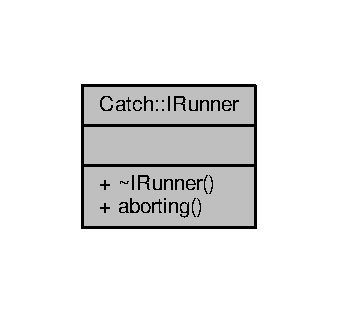
\includegraphics[width=162pt]{struct_catch_1_1_i_runner__coll__graph}
\end{center}
\end{figure}
\subsection*{Public Member Functions}
\begin{DoxyCompactItemize}
\item 
virtual \hyperlink{struct_catch_1_1_i_runner_a5f539a88a7772d68de8a2e4028774209}{$\sim$\-I\-Runner} ()
\item 
virtual bool \hyperlink{struct_catch_1_1_i_runner_a03713202dd2e041e30b8030088ab0116}{aborting} () const =0
\end{DoxyCompactItemize}


\subsection{Constructor \& Destructor Documentation}
\hypertarget{struct_catch_1_1_i_runner_a5f539a88a7772d68de8a2e4028774209}{\index{Catch\-::\-I\-Runner@{Catch\-::\-I\-Runner}!$\sim$\-I\-Runner@{$\sim$\-I\-Runner}}
\index{$\sim$\-I\-Runner@{$\sim$\-I\-Runner}!Catch::IRunner@{Catch\-::\-I\-Runner}}
\subsubsection[{$\sim$\-I\-Runner}]{\setlength{\rightskip}{0pt plus 5cm}virtual Catch\-::\-I\-Runner\-::$\sim$\-I\-Runner (
\begin{DoxyParamCaption}
{}
\end{DoxyParamCaption}
)\hspace{0.3cm}{\ttfamily [virtual]}}}\label{struct_catch_1_1_i_runner_a5f539a88a7772d68de8a2e4028774209}


\subsection{Member Function Documentation}
\hypertarget{struct_catch_1_1_i_runner_a03713202dd2e041e30b8030088ab0116}{\index{Catch\-::\-I\-Runner@{Catch\-::\-I\-Runner}!aborting@{aborting}}
\index{aborting@{aborting}!Catch::IRunner@{Catch\-::\-I\-Runner}}
\subsubsection[{aborting}]{\setlength{\rightskip}{0pt plus 5cm}virtual bool Catch\-::\-I\-Runner\-::aborting (
\begin{DoxyParamCaption}
{}
\end{DoxyParamCaption}
) const\hspace{0.3cm}{\ttfamily [pure virtual]}}}\label{struct_catch_1_1_i_runner_a03713202dd2e041e30b8030088ab0116}


The documentation for this struct was generated from the following file\-:\begin{DoxyCompactItemize}
\item 
\hyperlink{catch_8hpp}{catch.\-hpp}\end{DoxyCompactItemize}

\hypertarget{struct_catch_1_1is__range}{\section{Catch\-:\-:is\-\_\-range$<$ T $>$ Struct Template Reference}
\label{struct_catch_1_1is__range}\index{Catch\-::is\-\_\-range$<$ T $>$@{Catch\-::is\-\_\-range$<$ T $>$}}
}


{\ttfamily \#include $<$catch.\-hpp$>$}



Collaboration diagram for Catch\-:\-:is\-\_\-range$<$ T $>$\-:
\nopagebreak
\begin{figure}[H]
\begin{center}
\leavevmode
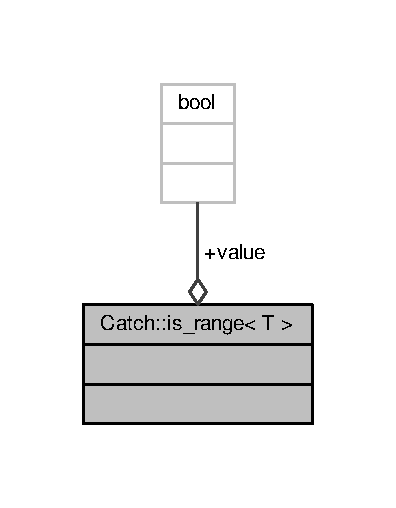
\includegraphics[width=190pt]{struct_catch_1_1is__range__coll__graph}
\end{center}
\end{figure}
\subsection*{Static Public Attributes}
\begin{DoxyCompactItemize}
\item 
static const bool \hyperlink{struct_catch_1_1is__range_afaec39e819c3956829cbbd00feba11be}{value}
\end{DoxyCompactItemize}


\subsection{Member Data Documentation}
\hypertarget{struct_catch_1_1is__range_afaec39e819c3956829cbbd00feba11be}{\index{Catch\-::is\-\_\-range@{Catch\-::is\-\_\-range}!value@{value}}
\index{value@{value}!Catch::is_range@{Catch\-::is\-\_\-range}}
\subsubsection[{value}]{\setlength{\rightskip}{0pt plus 5cm}template$<$typename T $>$ const bool {\bf Catch\-::is\-\_\-range}$<$ T $>$\-::value\hspace{0.3cm}{\ttfamily [static]}}}\label{struct_catch_1_1is__range_afaec39e819c3956829cbbd00feba11be}
{\bfseries Initial value\-:}
\begin{DoxyCode}
=
            !std::is\_same<decltype(begin(std::declval<T>())), not\_this\_one>::
      \hyperlink{struct_catch_1_1is__range_afaec39e819c3956829cbbd00feba11be}{value} &&
            !std::is\_same<decltype(\hyperlink{namespace_catch_a71fef6a57614eb2d9751f8586ff6de6a}{end}(std::declval<T>())), not\_this\_one>
      \hyperlink{struct_catch_1_1is__range_afaec39e819c3956829cbbd00feba11be}{::value}
\end{DoxyCode}


The documentation for this struct was generated from the following file\-:\begin{DoxyCompactItemize}
\item 
\hyperlink{catch_8hpp}{catch.\-hpp}\end{DoxyCompactItemize}

\hypertarget{class_catch_1_1_detail_1_1_is_stream_insertable}{\section{Catch\-:\-:Detail\-:\-:Is\-Stream\-Insertable$<$ T $>$ Class Template Reference}
\label{class_catch_1_1_detail_1_1_is_stream_insertable}\index{Catch\-::\-Detail\-::\-Is\-Stream\-Insertable$<$ T $>$@{Catch\-::\-Detail\-::\-Is\-Stream\-Insertable$<$ T $>$}}
}


{\ttfamily \#include $<$catch.\-hpp$>$}



Collaboration diagram for Catch\-:\-:Detail\-:\-:Is\-Stream\-Insertable$<$ T $>$\-:
\nopagebreak
\begin{figure}[H]
\begin{center}
\leavevmode
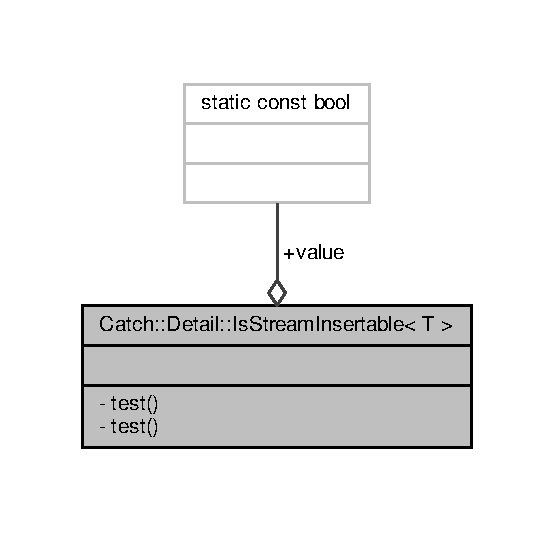
\includegraphics[width=266pt]{class_catch_1_1_detail_1_1_is_stream_insertable__coll__graph}
\end{center}
\end{figure}
\subsection*{Static Public Attributes}
\begin{DoxyCompactItemize}
\item 
static const bool \hyperlink{class_catch_1_1_detail_1_1_is_stream_insertable_a42818b09ae5851126a70ee263769e309}{value} = decltype(\hyperlink{class_catch_1_1_detail_1_1_is_stream_insertable_ac5981238a76d66e36b3d014aa870d15c}{test}$<$std\-::ostream, const T\&$>$(0))\-::value
\end{DoxyCompactItemize}
\subsection*{Static Private Member Functions}
\begin{DoxyCompactItemize}
\item 
{\footnotesize template$<$typename S\-S , typename T\-T $>$ }\\static auto \hyperlink{class_catch_1_1_detail_1_1_is_stream_insertable_ac5981238a76d66e36b3d014aa870d15c}{test} (int) -\/$>$ decltype(std\-::declval$<$ S\-S \& $>$()$<$$<$ std\-::declval$<$ T\-T $>$(), std\-::true\-\_\-type())
\item 
{\footnotesize template$<$typename , typename $>$ }\\static auto \hyperlink{class_catch_1_1_detail_1_1_is_stream_insertable_ac5761375646929916dc5e165d44cd3d9}{test} (...) -\/$>$ std\-::false\-\_\-type
\end{DoxyCompactItemize}


\subsection{Member Function Documentation}
\hypertarget{class_catch_1_1_detail_1_1_is_stream_insertable_ac5981238a76d66e36b3d014aa870d15c}{\index{Catch\-::\-Detail\-::\-Is\-Stream\-Insertable@{Catch\-::\-Detail\-::\-Is\-Stream\-Insertable}!test@{test}}
\index{test@{test}!Catch::Detail::IsStreamInsertable@{Catch\-::\-Detail\-::\-Is\-Stream\-Insertable}}
\subsubsection[{test}]{\setlength{\rightskip}{0pt plus 5cm}template$<$typename T $>$ template$<$typename S\-S , typename T\-T $>$ static auto {\bf Catch\-::\-Detail\-::\-Is\-Stream\-Insertable}$<$ T $>$\-::test (
\begin{DoxyParamCaption}
\item[{int}]{}
\end{DoxyParamCaption}
) -\/$>$  decltype(std\-::declval$<$ S\-S \& $>$()$<$$<$ std\-::declval$<$ T\-T $>$(), std\-::true\-\_\-type())\hspace{0.3cm}{\ttfamily [static]}, {\ttfamily [private]}}}\label{class_catch_1_1_detail_1_1_is_stream_insertable_ac5981238a76d66e36b3d014aa870d15c}
\hypertarget{class_catch_1_1_detail_1_1_is_stream_insertable_ac5761375646929916dc5e165d44cd3d9}{\index{Catch\-::\-Detail\-::\-Is\-Stream\-Insertable@{Catch\-::\-Detail\-::\-Is\-Stream\-Insertable}!test@{test}}
\index{test@{test}!Catch::Detail::IsStreamInsertable@{Catch\-::\-Detail\-::\-Is\-Stream\-Insertable}}
\subsubsection[{test}]{\setlength{\rightskip}{0pt plus 5cm}template$<$typename T $>$ template$<$typename , typename $>$ static auto {\bf Catch\-::\-Detail\-::\-Is\-Stream\-Insertable}$<$ T $>$\-::test (
\begin{DoxyParamCaption}
\item[{}]{...}
\end{DoxyParamCaption}
) -\/$>$  std\-::false\-\_\-type\hspace{0.3cm}{\ttfamily [static]}, {\ttfamily [private]}}}\label{class_catch_1_1_detail_1_1_is_stream_insertable_ac5761375646929916dc5e165d44cd3d9}


\subsection{Member Data Documentation}
\hypertarget{class_catch_1_1_detail_1_1_is_stream_insertable_a42818b09ae5851126a70ee263769e309}{\index{Catch\-::\-Detail\-::\-Is\-Stream\-Insertable@{Catch\-::\-Detail\-::\-Is\-Stream\-Insertable}!value@{value}}
\index{value@{value}!Catch::Detail::IsStreamInsertable@{Catch\-::\-Detail\-::\-Is\-Stream\-Insertable}}
\subsubsection[{value}]{\setlength{\rightskip}{0pt plus 5cm}template$<$typename T $>$ const bool {\bf Catch\-::\-Detail\-::\-Is\-Stream\-Insertable}$<$ T $>$\-::value = decltype({\bf test}$<$std\-::ostream, const T\&$>$(0))\-::value\hspace{0.3cm}{\ttfamily [static]}}}\label{class_catch_1_1_detail_1_1_is_stream_insertable_a42818b09ae5851126a70ee263769e309}


The documentation for this class was generated from the following file\-:\begin{DoxyCompactItemize}
\item 
\hyperlink{catch_8hpp}{catch.\-hpp}\end{DoxyCompactItemize}

\hypertarget{struct_catch_1_1_i_stream}{\section{Catch\-:\-:I\-Stream Struct Reference}
\label{struct_catch_1_1_i_stream}\index{Catch\-::\-I\-Stream@{Catch\-::\-I\-Stream}}
}


{\ttfamily \#include $<$catch.\-hpp$>$}



Collaboration diagram for Catch\-:\-:I\-Stream\-:
\nopagebreak
\begin{figure}[H]
\begin{center}
\leavevmode
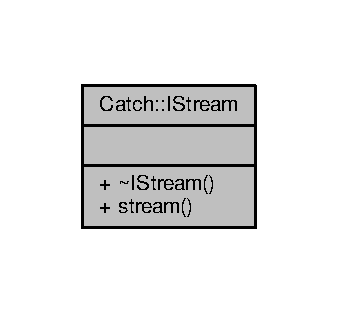
\includegraphics[width=162pt]{struct_catch_1_1_i_stream__coll__graph}
\end{center}
\end{figure}
\subsection*{Public Member Functions}
\begin{DoxyCompactItemize}
\item 
virtual \hyperlink{struct_catch_1_1_i_stream_a344a88d0e5fc1f727f5801c72b4a4e2a}{$\sim$\-I\-Stream} ()
\item 
virtual std\-::ostream \& \hyperlink{struct_catch_1_1_i_stream_a55a9ddbe250261ff38642f480ebdd902}{stream} () const =0
\end{DoxyCompactItemize}


\subsection{Constructor \& Destructor Documentation}
\hypertarget{struct_catch_1_1_i_stream_a344a88d0e5fc1f727f5801c72b4a4e2a}{\index{Catch\-::\-I\-Stream@{Catch\-::\-I\-Stream}!$\sim$\-I\-Stream@{$\sim$\-I\-Stream}}
\index{$\sim$\-I\-Stream@{$\sim$\-I\-Stream}!Catch::IStream@{Catch\-::\-I\-Stream}}
\subsubsection[{$\sim$\-I\-Stream}]{\setlength{\rightskip}{0pt plus 5cm}virtual Catch\-::\-I\-Stream\-::$\sim$\-I\-Stream (
\begin{DoxyParamCaption}
{}
\end{DoxyParamCaption}
)\hspace{0.3cm}{\ttfamily [virtual]}}}\label{struct_catch_1_1_i_stream_a344a88d0e5fc1f727f5801c72b4a4e2a}


\subsection{Member Function Documentation}
\hypertarget{struct_catch_1_1_i_stream_a55a9ddbe250261ff38642f480ebdd902}{\index{Catch\-::\-I\-Stream@{Catch\-::\-I\-Stream}!stream@{stream}}
\index{stream@{stream}!Catch::IStream@{Catch\-::\-I\-Stream}}
\subsubsection[{stream}]{\setlength{\rightskip}{0pt plus 5cm}virtual std\-::ostream\& Catch\-::\-I\-Stream\-::stream (
\begin{DoxyParamCaption}
{}
\end{DoxyParamCaption}
) const\hspace{0.3cm}{\ttfamily [pure virtual]}}}\label{struct_catch_1_1_i_stream_a55a9ddbe250261ff38642f480ebdd902}


The documentation for this struct was generated from the following file\-:\begin{DoxyCompactItemize}
\item 
\hyperlink{catch_8hpp}{catch.\-hpp}\end{DoxyCompactItemize}

\hypertarget{struct_catch_1_1_i_test_case_registry}{\section{Catch\-:\-:I\-Test\-Case\-Registry Struct Reference}
\label{struct_catch_1_1_i_test_case_registry}\index{Catch\-::\-I\-Test\-Case\-Registry@{Catch\-::\-I\-Test\-Case\-Registry}}
}


{\ttfamily \#include $<$catch.\-hpp$>$}



Collaboration diagram for Catch\-:\-:I\-Test\-Case\-Registry\-:
\nopagebreak
\begin{figure}[H]
\begin{center}
\leavevmode
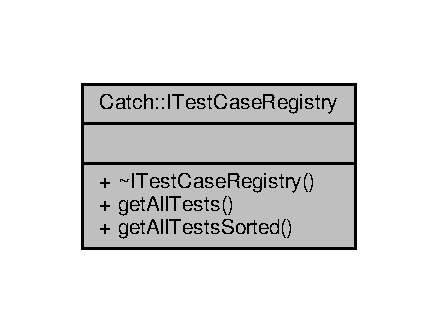
\includegraphics[width=210pt]{struct_catch_1_1_i_test_case_registry__coll__graph}
\end{center}
\end{figure}
\subsection*{Public Member Functions}
\begin{DoxyCompactItemize}
\item 
virtual \hyperlink{struct_catch_1_1_i_test_case_registry_ae14798f05ac8e2b18cff532849a4da81}{$\sim$\-I\-Test\-Case\-Registry} ()
\item 
virtual std\-::vector$<$ \hyperlink{class_catch_1_1_test_case}{Test\-Case} $>$\\*
 const \& \hyperlink{struct_catch_1_1_i_test_case_registry_ad6e4d4a621655123f73ae98cfeda063d}{get\-All\-Tests} () const =0
\item 
virtual std\-::vector$<$ \hyperlink{class_catch_1_1_test_case}{Test\-Case} $>$\\*
 const \& \hyperlink{struct_catch_1_1_i_test_case_registry_a33e46639d0319d35497c05bb5d02be5a}{get\-All\-Tests\-Sorted} (I\-Config const \&config) const =0
\end{DoxyCompactItemize}


\subsection{Constructor \& Destructor Documentation}
\hypertarget{struct_catch_1_1_i_test_case_registry_ae14798f05ac8e2b18cff532849a4da81}{\index{Catch\-::\-I\-Test\-Case\-Registry@{Catch\-::\-I\-Test\-Case\-Registry}!$\sim$\-I\-Test\-Case\-Registry@{$\sim$\-I\-Test\-Case\-Registry}}
\index{$\sim$\-I\-Test\-Case\-Registry@{$\sim$\-I\-Test\-Case\-Registry}!Catch::ITestCaseRegistry@{Catch\-::\-I\-Test\-Case\-Registry}}
\subsubsection[{$\sim$\-I\-Test\-Case\-Registry}]{\setlength{\rightskip}{0pt plus 5cm}virtual Catch\-::\-I\-Test\-Case\-Registry\-::$\sim$\-I\-Test\-Case\-Registry (
\begin{DoxyParamCaption}
{}
\end{DoxyParamCaption}
)\hspace{0.3cm}{\ttfamily [virtual]}}}\label{struct_catch_1_1_i_test_case_registry_ae14798f05ac8e2b18cff532849a4da81}


\subsection{Member Function Documentation}
\hypertarget{struct_catch_1_1_i_test_case_registry_ad6e4d4a621655123f73ae98cfeda063d}{\index{Catch\-::\-I\-Test\-Case\-Registry@{Catch\-::\-I\-Test\-Case\-Registry}!get\-All\-Tests@{get\-All\-Tests}}
\index{get\-All\-Tests@{get\-All\-Tests}!Catch::ITestCaseRegistry@{Catch\-::\-I\-Test\-Case\-Registry}}
\subsubsection[{get\-All\-Tests}]{\setlength{\rightskip}{0pt plus 5cm}virtual std\-::vector$<${\bf Test\-Case}$>$ const\& Catch\-::\-I\-Test\-Case\-Registry\-::get\-All\-Tests (
\begin{DoxyParamCaption}
{}
\end{DoxyParamCaption}
) const\hspace{0.3cm}{\ttfamily [pure virtual]}}}\label{struct_catch_1_1_i_test_case_registry_ad6e4d4a621655123f73ae98cfeda063d}
\hypertarget{struct_catch_1_1_i_test_case_registry_a33e46639d0319d35497c05bb5d02be5a}{\index{Catch\-::\-I\-Test\-Case\-Registry@{Catch\-::\-I\-Test\-Case\-Registry}!get\-All\-Tests\-Sorted@{get\-All\-Tests\-Sorted}}
\index{get\-All\-Tests\-Sorted@{get\-All\-Tests\-Sorted}!Catch::ITestCaseRegistry@{Catch\-::\-I\-Test\-Case\-Registry}}
\subsubsection[{get\-All\-Tests\-Sorted}]{\setlength{\rightskip}{0pt plus 5cm}virtual std\-::vector$<${\bf Test\-Case}$>$ const\& Catch\-::\-I\-Test\-Case\-Registry\-::get\-All\-Tests\-Sorted (
\begin{DoxyParamCaption}
\item[{I\-Config const \&}]{config}
\end{DoxyParamCaption}
) const\hspace{0.3cm}{\ttfamily [pure virtual]}}}\label{struct_catch_1_1_i_test_case_registry_a33e46639d0319d35497c05bb5d02be5a}


The documentation for this struct was generated from the following file\-:\begin{DoxyCompactItemize}
\item 
\hyperlink{catch_8hpp}{catch.\-hpp}\end{DoxyCompactItemize}

\hypertarget{struct_catch_1_1_i_test_invoker}{\section{Catch\-:\-:I\-Test\-Invoker Struct Reference}
\label{struct_catch_1_1_i_test_invoker}\index{Catch\-::\-I\-Test\-Invoker@{Catch\-::\-I\-Test\-Invoker}}
}


{\ttfamily \#include $<$catch.\-hpp$>$}



Inheritance diagram for Catch\-:\-:I\-Test\-Invoker\-:
\nopagebreak
\begin{figure}[H]
\begin{center}
\leavevmode
\includegraphics[width=250pt]{struct_catch_1_1_i_test_invoker__inherit__graph}
\end{center}
\end{figure}


Collaboration diagram for Catch\-:\-:I\-Test\-Invoker\-:
\nopagebreak
\begin{figure}[H]
\begin{center}
\leavevmode
\includegraphics[width=184pt]{struct_catch_1_1_i_test_invoker__coll__graph}
\end{center}
\end{figure}
\subsection*{Public Member Functions}
\begin{DoxyCompactItemize}
\item 
virtual void \hyperlink{struct_catch_1_1_i_test_invoker_a6fcd5c5b67d6d5ade6491ff33411ca7f}{invoke} () const =0
\item 
virtual \hyperlink{struct_catch_1_1_i_test_invoker_a2c89f3eece5b1b677243766e409bd831}{$\sim$\-I\-Test\-Invoker} ()
\end{DoxyCompactItemize}


\subsection{Constructor \& Destructor Documentation}
\hypertarget{struct_catch_1_1_i_test_invoker_a2c89f3eece5b1b677243766e409bd831}{\index{Catch\-::\-I\-Test\-Invoker@{Catch\-::\-I\-Test\-Invoker}!$\sim$\-I\-Test\-Invoker@{$\sim$\-I\-Test\-Invoker}}
\index{$\sim$\-I\-Test\-Invoker@{$\sim$\-I\-Test\-Invoker}!Catch::ITestInvoker@{Catch\-::\-I\-Test\-Invoker}}
\subsubsection[{$\sim$\-I\-Test\-Invoker}]{\setlength{\rightskip}{0pt plus 5cm}virtual Catch\-::\-I\-Test\-Invoker\-::$\sim$\-I\-Test\-Invoker (
\begin{DoxyParamCaption}
{}
\end{DoxyParamCaption}
)\hspace{0.3cm}{\ttfamily [virtual]}}}\label{struct_catch_1_1_i_test_invoker_a2c89f3eece5b1b677243766e409bd831}


\subsection{Member Function Documentation}
\hypertarget{struct_catch_1_1_i_test_invoker_a6fcd5c5b67d6d5ade6491ff33411ca7f}{\index{Catch\-::\-I\-Test\-Invoker@{Catch\-::\-I\-Test\-Invoker}!invoke@{invoke}}
\index{invoke@{invoke}!Catch::ITestInvoker@{Catch\-::\-I\-Test\-Invoker}}
\subsubsection[{invoke}]{\setlength{\rightskip}{0pt plus 5cm}virtual void Catch\-::\-I\-Test\-Invoker\-::invoke (
\begin{DoxyParamCaption}
{}
\end{DoxyParamCaption}
) const\hspace{0.3cm}{\ttfamily [pure virtual]}}}\label{struct_catch_1_1_i_test_invoker_a6fcd5c5b67d6d5ade6491ff33411ca7f}


Implemented in \hyperlink{class_catch_1_1_test_invoker_as_method_a8115a06efe273f4112ec0b5452c1b5f2}{Catch\-::\-Test\-Invoker\-As\-Method$<$ C $>$}.



The documentation for this struct was generated from the following file\-:\begin{DoxyCompactItemize}
\item 
\hyperlink{catch_8hpp}{catch.\-hpp}\end{DoxyCompactItemize}

\hypertarget{struct_catch_1_1_i_transient_expression}{\section{Catch\-:\-:I\-Transient\-Expression Struct Reference}
\label{struct_catch_1_1_i_transient_expression}\index{Catch\-::\-I\-Transient\-Expression@{Catch\-::\-I\-Transient\-Expression}}
}


{\ttfamily \#include $<$catch.\-hpp$>$}



Inheritance diagram for Catch\-:\-:I\-Transient\-Expression\-:
\nopagebreak
\begin{figure}[H]
\begin{center}
\leavevmode
\includegraphics[width=350pt]{struct_catch_1_1_i_transient_expression__inherit__graph}
\end{center}
\end{figure}


Collaboration diagram for Catch\-:\-:I\-Transient\-Expression\-:
\nopagebreak
\begin{figure}[H]
\begin{center}
\leavevmode
\includegraphics[width=274pt]{struct_catch_1_1_i_transient_expression__coll__graph}
\end{center}
\end{figure}
\subsection*{Public Member Functions}
\begin{DoxyCompactItemize}
\item 
auto \hyperlink{struct_catch_1_1_i_transient_expression_a3b436e13a0a6d3522bbf70d4e31deb22}{is\-Binary\-Expression} () const -\/$>$ bool
\item 
auto \hyperlink{struct_catch_1_1_i_transient_expression_a101c7db86c87eff93a8ff496720e6320}{get\-Result} () const -\/$>$ bool
\item 
virtual void \hyperlink{struct_catch_1_1_i_transient_expression_aabe1889df9c6e639a24afb08d8a0fe9e}{stream\-Reconstructed\-Expression} (std\-::ostream \&os) const =0
\item 
\hyperlink{struct_catch_1_1_i_transient_expression_aafe69572b7ed884e63ec81f58d4afd8c}{I\-Transient\-Expression} (bool \hyperlink{struct_catch_1_1_i_transient_expression_a3b436e13a0a6d3522bbf70d4e31deb22}{is\-Binary\-Expression}, bool result)
\item 
virtual \hyperlink{struct_catch_1_1_i_transient_expression_aeadf426de589938c4964fe4068eeee77}{$\sim$\-I\-Transient\-Expression} ()
\end{DoxyCompactItemize}
\subsection*{Public Attributes}
\begin{DoxyCompactItemize}
\item 
bool \hyperlink{struct_catch_1_1_i_transient_expression_a75ce48da824d514d08152d396abb28d8}{m\-\_\-is\-Binary\-Expression}
\item 
bool \hyperlink{struct_catch_1_1_i_transient_expression_a4646e2b5e0156e913653ec3b9b60c942}{m\-\_\-result}
\end{DoxyCompactItemize}


\subsection{Constructor \& Destructor Documentation}
\hypertarget{struct_catch_1_1_i_transient_expression_aafe69572b7ed884e63ec81f58d4afd8c}{\index{Catch\-::\-I\-Transient\-Expression@{Catch\-::\-I\-Transient\-Expression}!I\-Transient\-Expression@{I\-Transient\-Expression}}
\index{I\-Transient\-Expression@{I\-Transient\-Expression}!Catch::ITransientExpression@{Catch\-::\-I\-Transient\-Expression}}
\subsubsection[{I\-Transient\-Expression}]{\setlength{\rightskip}{0pt plus 5cm}Catch\-::\-I\-Transient\-Expression\-::\-I\-Transient\-Expression (
\begin{DoxyParamCaption}
\item[{bool}]{is\-Binary\-Expression, }
\item[{bool}]{result}
\end{DoxyParamCaption}
)\hspace{0.3cm}{\ttfamily [inline]}}}\label{struct_catch_1_1_i_transient_expression_aafe69572b7ed884e63ec81f58d4afd8c}

\begin{DoxyCode}
1307             : \hyperlink{struct_catch_1_1_i_transient_expression_a75ce48da824d514d08152d396abb28d8}{m\_isBinaryExpression}(\hyperlink{struct_catch_1_1_i_transient_expression_a3b436e13a0a6d3522bbf70d4e31deb22}{isBinaryExpression}),
1308             \hyperlink{struct_catch_1_1_i_transient_expression_a4646e2b5e0156e913653ec3b9b60c942}{m\_result}(result)
1309         \{\}
\end{DoxyCode}
\hypertarget{struct_catch_1_1_i_transient_expression_aeadf426de589938c4964fe4068eeee77}{\index{Catch\-::\-I\-Transient\-Expression@{Catch\-::\-I\-Transient\-Expression}!$\sim$\-I\-Transient\-Expression@{$\sim$\-I\-Transient\-Expression}}
\index{$\sim$\-I\-Transient\-Expression@{$\sim$\-I\-Transient\-Expression}!Catch::ITransientExpression@{Catch\-::\-I\-Transient\-Expression}}
\subsubsection[{$\sim$\-I\-Transient\-Expression}]{\setlength{\rightskip}{0pt plus 5cm}virtual Catch\-::\-I\-Transient\-Expression\-::$\sim$\-I\-Transient\-Expression (
\begin{DoxyParamCaption}
{}
\end{DoxyParamCaption}
)\hspace{0.3cm}{\ttfamily [virtual]}}}\label{struct_catch_1_1_i_transient_expression_aeadf426de589938c4964fe4068eeee77}


\subsection{Member Function Documentation}
\hypertarget{struct_catch_1_1_i_transient_expression_a101c7db86c87eff93a8ff496720e6320}{\index{Catch\-::\-I\-Transient\-Expression@{Catch\-::\-I\-Transient\-Expression}!get\-Result@{get\-Result}}
\index{get\-Result@{get\-Result}!Catch::ITransientExpression@{Catch\-::\-I\-Transient\-Expression}}
\subsubsection[{get\-Result}]{\setlength{\rightskip}{0pt plus 5cm}auto Catch\-::\-I\-Transient\-Expression\-::get\-Result (
\begin{DoxyParamCaption}
{}
\end{DoxyParamCaption}
) const -\/$>$ bool \hspace{0.3cm}{\ttfamily [inline]}}}\label{struct_catch_1_1_i_transient_expression_a101c7db86c87eff93a8ff496720e6320}

\begin{DoxyCode}
1303 \{ \textcolor{keywordflow}{return} \hyperlink{struct_catch_1_1_i_transient_expression_a4646e2b5e0156e913653ec3b9b60c942}{m\_result}; \}
\end{DoxyCode}
\hypertarget{struct_catch_1_1_i_transient_expression_a3b436e13a0a6d3522bbf70d4e31deb22}{\index{Catch\-::\-I\-Transient\-Expression@{Catch\-::\-I\-Transient\-Expression}!is\-Binary\-Expression@{is\-Binary\-Expression}}
\index{is\-Binary\-Expression@{is\-Binary\-Expression}!Catch::ITransientExpression@{Catch\-::\-I\-Transient\-Expression}}
\subsubsection[{is\-Binary\-Expression}]{\setlength{\rightskip}{0pt plus 5cm}auto Catch\-::\-I\-Transient\-Expression\-::is\-Binary\-Expression (
\begin{DoxyParamCaption}
{}
\end{DoxyParamCaption}
) const -\/$>$ bool \hspace{0.3cm}{\ttfamily [inline]}}}\label{struct_catch_1_1_i_transient_expression_a3b436e13a0a6d3522bbf70d4e31deb22}

\begin{DoxyCode}
1302 \{ \textcolor{keywordflow}{return} \hyperlink{struct_catch_1_1_i_transient_expression_a75ce48da824d514d08152d396abb28d8}{m\_isBinaryExpression}; \}
\end{DoxyCode}
\hypertarget{struct_catch_1_1_i_transient_expression_aabe1889df9c6e639a24afb08d8a0fe9e}{\index{Catch\-::\-I\-Transient\-Expression@{Catch\-::\-I\-Transient\-Expression}!stream\-Reconstructed\-Expression@{stream\-Reconstructed\-Expression}}
\index{stream\-Reconstructed\-Expression@{stream\-Reconstructed\-Expression}!Catch::ITransientExpression@{Catch\-::\-I\-Transient\-Expression}}
\subsubsection[{stream\-Reconstructed\-Expression}]{\setlength{\rightskip}{0pt plus 5cm}virtual void Catch\-::\-I\-Transient\-Expression\-::stream\-Reconstructed\-Expression (
\begin{DoxyParamCaption}
\item[{std\-::ostream \&}]{os}
\end{DoxyParamCaption}
) const\hspace{0.3cm}{\ttfamily [pure virtual]}}}\label{struct_catch_1_1_i_transient_expression_aabe1889df9c6e639a24afb08d8a0fe9e}


Implemented in \hyperlink{class_catch_1_1_match_expr_ad3e41adb597750b2219bb37e51185629}{Catch\-::\-Match\-Expr$<$ Arg\-T, Matcher\-T $>$}, \hyperlink{class_catch_1_1_unary_expr_aaabf30455a996c80675c0f388a6e4110}{Catch\-::\-Unary\-Expr$<$ Lhs\-T $>$}, and \hyperlink{class_catch_1_1_binary_expr_af998022712d4bd3e4fc7ab9b8a38b445}{Catch\-::\-Binary\-Expr$<$ Lhs\-T, Rhs\-T $>$}.



\subsection{Member Data Documentation}
\hypertarget{struct_catch_1_1_i_transient_expression_a75ce48da824d514d08152d396abb28d8}{\index{Catch\-::\-I\-Transient\-Expression@{Catch\-::\-I\-Transient\-Expression}!m\-\_\-is\-Binary\-Expression@{m\-\_\-is\-Binary\-Expression}}
\index{m\-\_\-is\-Binary\-Expression@{m\-\_\-is\-Binary\-Expression}!Catch::ITransientExpression@{Catch\-::\-I\-Transient\-Expression}}
\subsubsection[{m\-\_\-is\-Binary\-Expression}]{\setlength{\rightskip}{0pt plus 5cm}bool Catch\-::\-I\-Transient\-Expression\-::m\-\_\-is\-Binary\-Expression}}\label{struct_catch_1_1_i_transient_expression_a75ce48da824d514d08152d396abb28d8}
\hypertarget{struct_catch_1_1_i_transient_expression_a4646e2b5e0156e913653ec3b9b60c942}{\index{Catch\-::\-I\-Transient\-Expression@{Catch\-::\-I\-Transient\-Expression}!m\-\_\-result@{m\-\_\-result}}
\index{m\-\_\-result@{m\-\_\-result}!Catch::ITransientExpression@{Catch\-::\-I\-Transient\-Expression}}
\subsubsection[{m\-\_\-result}]{\setlength{\rightskip}{0pt plus 5cm}bool Catch\-::\-I\-Transient\-Expression\-::m\-\_\-result}}\label{struct_catch_1_1_i_transient_expression_a4646e2b5e0156e913653ec3b9b60c942}


The documentation for this struct was generated from the following file\-:\begin{DoxyCompactItemize}
\item 
\hyperlink{catch_8hpp}{catch.\-hpp}\end{DoxyCompactItemize}

\hypertarget{class_catch_1_1_lazy_expression}{\section{Catch\-:\-:Lazy\-Expression Class Reference}
\label{class_catch_1_1_lazy_expression}\index{Catch\-::\-Lazy\-Expression@{Catch\-::\-Lazy\-Expression}}
}


{\ttfamily \#include $<$catch.\-hpp$>$}



Collaboration diagram for Catch\-:\-:Lazy\-Expression\-:
\nopagebreak
\begin{figure}[H]
\begin{center}
\leavevmode
\includegraphics[width=345pt]{class_catch_1_1_lazy_expression__coll__graph}
\end{center}
\end{figure}
\subsection*{Public Member Functions}
\begin{DoxyCompactItemize}
\item 
\hyperlink{class_catch_1_1_lazy_expression_a47186c2487bd4bf871e870ba8048553a}{Lazy\-Expression} (bool is\-Negated)
\item 
\hyperlink{class_catch_1_1_lazy_expression_ab82d5e94df0e159b018fbde0170e46f8}{Lazy\-Expression} (\hyperlink{class_catch_1_1_lazy_expression}{Lazy\-Expression} const \&other)
\item 
\hyperlink{class_catch_1_1_lazy_expression}{Lazy\-Expression} \& \hyperlink{class_catch_1_1_lazy_expression_ae4ae00d4f36f084c369f2da36565a822}{operator=} (\hyperlink{class_catch_1_1_lazy_expression}{Lazy\-Expression} const \&)=delete
\item 
\hyperlink{class_catch_1_1_lazy_expression_a5f3541ec933ad977b6a10ddf61b45adc}{operator bool} () const 
\end{DoxyCompactItemize}
\subsection*{Private Attributes}
\begin{DoxyCompactItemize}
\item 
\hyperlink{struct_catch_1_1_i_transient_expression}{I\-Transient\-Expression} const $\ast$ \hyperlink{class_catch_1_1_lazy_expression_a5a9ce4c2401a262c21b4e107551180bc}{m\-\_\-transient\-Expression} = nullptr
\item 
bool \hyperlink{class_catch_1_1_lazy_expression_a975fdfe2bb139512024bb479d478425e}{m\-\_\-is\-Negated}
\end{DoxyCompactItemize}
\subsection*{Friends}
\begin{DoxyCompactItemize}
\item 
class \hyperlink{class_catch_1_1_lazy_expression_a4301a3aa57b612dd8b6ef8461742ecab}{Assertion\-Handler}
\item 
struct \hyperlink{class_catch_1_1_lazy_expression_a64019eb137f5ce447cdc71cb80b6e7a4}{Assertion\-Stats}
\item 
class \hyperlink{class_catch_1_1_lazy_expression_af3aa096bb29a772bc534830f29a2ce7a}{Run\-Context}
\item 
auto \hyperlink{class_catch_1_1_lazy_expression_aa01086581cab2fcd2d4580b8fa787dfc}{operator$<$$<$} (std\-::ostream \&os, \hyperlink{class_catch_1_1_lazy_expression}{Lazy\-Expression} const \&lazy\-Expr) -\/$>$ std\-::ostream \&
\end{DoxyCompactItemize}


\subsection{Constructor \& Destructor Documentation}
\hypertarget{class_catch_1_1_lazy_expression_a47186c2487bd4bf871e870ba8048553a}{\index{Catch\-::\-Lazy\-Expression@{Catch\-::\-Lazy\-Expression}!Lazy\-Expression@{Lazy\-Expression}}
\index{Lazy\-Expression@{Lazy\-Expression}!Catch::LazyExpression@{Catch\-::\-Lazy\-Expression}}
\subsubsection[{Lazy\-Expression}]{\setlength{\rightskip}{0pt plus 5cm}Catch\-::\-Lazy\-Expression\-::\-Lazy\-Expression (
\begin{DoxyParamCaption}
\item[{bool}]{is\-Negated}
\end{DoxyParamCaption}
)}}\label{class_catch_1_1_lazy_expression_a47186c2487bd4bf871e870ba8048553a}
\hypertarget{class_catch_1_1_lazy_expression_ab82d5e94df0e159b018fbde0170e46f8}{\index{Catch\-::\-Lazy\-Expression@{Catch\-::\-Lazy\-Expression}!Lazy\-Expression@{Lazy\-Expression}}
\index{Lazy\-Expression@{Lazy\-Expression}!Catch::LazyExpression@{Catch\-::\-Lazy\-Expression}}
\subsubsection[{Lazy\-Expression}]{\setlength{\rightskip}{0pt plus 5cm}Catch\-::\-Lazy\-Expression\-::\-Lazy\-Expression (
\begin{DoxyParamCaption}
\item[{{\bf Lazy\-Expression} const \&}]{other}
\end{DoxyParamCaption}
)}}\label{class_catch_1_1_lazy_expression_ab82d5e94df0e159b018fbde0170e46f8}


\subsection{Member Function Documentation}
\hypertarget{class_catch_1_1_lazy_expression_a5f3541ec933ad977b6a10ddf61b45adc}{\index{Catch\-::\-Lazy\-Expression@{Catch\-::\-Lazy\-Expression}!operator bool@{operator bool}}
\index{operator bool@{operator bool}!Catch::LazyExpression@{Catch\-::\-Lazy\-Expression}}
\subsubsection[{operator bool}]{\setlength{\rightskip}{0pt plus 5cm}Catch\-::\-Lazy\-Expression\-::operator bool (
\begin{DoxyParamCaption}
{}
\end{DoxyParamCaption}
) const\hspace{0.3cm}{\ttfamily [explicit]}}}\label{class_catch_1_1_lazy_expression_a5f3541ec933ad977b6a10ddf61b45adc}
\hypertarget{class_catch_1_1_lazy_expression_ae4ae00d4f36f084c369f2da36565a822}{\index{Catch\-::\-Lazy\-Expression@{Catch\-::\-Lazy\-Expression}!operator=@{operator=}}
\index{operator=@{operator=}!Catch::LazyExpression@{Catch\-::\-Lazy\-Expression}}
\subsubsection[{operator=}]{\setlength{\rightskip}{0pt plus 5cm}{\bf Lazy\-Expression}\& Catch\-::\-Lazy\-Expression\-::operator= (
\begin{DoxyParamCaption}
\item[{{\bf Lazy\-Expression} const \&}]{}
\end{DoxyParamCaption}
)\hspace{0.3cm}{\ttfamily [delete]}}}\label{class_catch_1_1_lazy_expression_ae4ae00d4f36f084c369f2da36565a822}


\subsection{Friends And Related Function Documentation}
\hypertarget{class_catch_1_1_lazy_expression_a4301a3aa57b612dd8b6ef8461742ecab}{\index{Catch\-::\-Lazy\-Expression@{Catch\-::\-Lazy\-Expression}!Assertion\-Handler@{Assertion\-Handler}}
\index{Assertion\-Handler@{Assertion\-Handler}!Catch::LazyExpression@{Catch\-::\-Lazy\-Expression}}
\subsubsection[{Assertion\-Handler}]{\setlength{\rightskip}{0pt plus 5cm}friend class {\bf Assertion\-Handler}\hspace{0.3cm}{\ttfamily [friend]}}}\label{class_catch_1_1_lazy_expression_a4301a3aa57b612dd8b6ef8461742ecab}
\hypertarget{class_catch_1_1_lazy_expression_a64019eb137f5ce447cdc71cb80b6e7a4}{\index{Catch\-::\-Lazy\-Expression@{Catch\-::\-Lazy\-Expression}!Assertion\-Stats@{Assertion\-Stats}}
\index{Assertion\-Stats@{Assertion\-Stats}!Catch::LazyExpression@{Catch\-::\-Lazy\-Expression}}
\subsubsection[{Assertion\-Stats}]{\setlength{\rightskip}{0pt plus 5cm}friend struct Assertion\-Stats\hspace{0.3cm}{\ttfamily [friend]}}}\label{class_catch_1_1_lazy_expression_a64019eb137f5ce447cdc71cb80b6e7a4}
\hypertarget{class_catch_1_1_lazy_expression_aa01086581cab2fcd2d4580b8fa787dfc}{\index{Catch\-::\-Lazy\-Expression@{Catch\-::\-Lazy\-Expression}!operator$<$$<$@{operator$<$$<$}}
\index{operator$<$$<$@{operator$<$$<$}!Catch::LazyExpression@{Catch\-::\-Lazy\-Expression}}
\subsubsection[{operator$<$$<$}]{\setlength{\rightskip}{0pt plus 5cm}auto operator$<$$<$ (
\begin{DoxyParamCaption}
\item[{std\-::ostream \&}]{os, }
\item[{{\bf Lazy\-Expression} const \&}]{lazy\-Expr}
\end{DoxyParamCaption}
) -\/$>$  std\-::ostream \&\hspace{0.3cm}{\ttfamily [friend]}}}\label{class_catch_1_1_lazy_expression_aa01086581cab2fcd2d4580b8fa787dfc}
\hypertarget{class_catch_1_1_lazy_expression_af3aa096bb29a772bc534830f29a2ce7a}{\index{Catch\-::\-Lazy\-Expression@{Catch\-::\-Lazy\-Expression}!Run\-Context@{Run\-Context}}
\index{Run\-Context@{Run\-Context}!Catch::LazyExpression@{Catch\-::\-Lazy\-Expression}}
\subsubsection[{Run\-Context}]{\setlength{\rightskip}{0pt plus 5cm}friend class Run\-Context\hspace{0.3cm}{\ttfamily [friend]}}}\label{class_catch_1_1_lazy_expression_af3aa096bb29a772bc534830f29a2ce7a}


\subsection{Member Data Documentation}
\hypertarget{class_catch_1_1_lazy_expression_a975fdfe2bb139512024bb479d478425e}{\index{Catch\-::\-Lazy\-Expression@{Catch\-::\-Lazy\-Expression}!m\-\_\-is\-Negated@{m\-\_\-is\-Negated}}
\index{m\-\_\-is\-Negated@{m\-\_\-is\-Negated}!Catch::LazyExpression@{Catch\-::\-Lazy\-Expression}}
\subsubsection[{m\-\_\-is\-Negated}]{\setlength{\rightskip}{0pt plus 5cm}bool Catch\-::\-Lazy\-Expression\-::m\-\_\-is\-Negated\hspace{0.3cm}{\ttfamily [private]}}}\label{class_catch_1_1_lazy_expression_a975fdfe2bb139512024bb479d478425e}
\hypertarget{class_catch_1_1_lazy_expression_a5a9ce4c2401a262c21b4e107551180bc}{\index{Catch\-::\-Lazy\-Expression@{Catch\-::\-Lazy\-Expression}!m\-\_\-transient\-Expression@{m\-\_\-transient\-Expression}}
\index{m\-\_\-transient\-Expression@{m\-\_\-transient\-Expression}!Catch::LazyExpression@{Catch\-::\-Lazy\-Expression}}
\subsubsection[{m\-\_\-transient\-Expression}]{\setlength{\rightskip}{0pt plus 5cm}{\bf I\-Transient\-Expression} const$\ast$ Catch\-::\-Lazy\-Expression\-::m\-\_\-transient\-Expression = nullptr\hspace{0.3cm}{\ttfamily [private]}}}\label{class_catch_1_1_lazy_expression_a5a9ce4c2401a262c21b4e107551180bc}


The documentation for this class was generated from the following file\-:\begin{DoxyCompactItemize}
\item 
\hyperlink{catch_8hpp}{catch.\-hpp}\end{DoxyCompactItemize}

\hypertarget{struct_catch_1_1_matchers_1_1_impl_1_1_match_all_of}{\section{Catch\-:\-:Matchers\-:\-:Impl\-:\-:Match\-All\-Of$<$ Arg\-T $>$ Struct Template Reference}
\label{struct_catch_1_1_matchers_1_1_impl_1_1_match_all_of}\index{Catch\-::\-Matchers\-::\-Impl\-::\-Match\-All\-Of$<$ Arg\-T $>$@{Catch\-::\-Matchers\-::\-Impl\-::\-Match\-All\-Of$<$ Arg\-T $>$}}
}


{\ttfamily \#include $<$catch.\-hpp$>$}



Inheritance diagram for Catch\-:\-:Matchers\-:\-:Impl\-:\-:Match\-All\-Of$<$ Arg\-T $>$\-:
\nopagebreak
\begin{figure}[H]
\begin{center}
\leavevmode
\includegraphics[height=550pt]{struct_catch_1_1_matchers_1_1_impl_1_1_match_all_of__inherit__graph}
\end{center}
\end{figure}


Collaboration diagram for Catch\-:\-:Matchers\-:\-:Impl\-:\-:Match\-All\-Of$<$ Arg\-T $>$\-:
\nopagebreak
\begin{figure}[H]
\begin{center}
\leavevmode
\includegraphics[height=550pt]{struct_catch_1_1_matchers_1_1_impl_1_1_match_all_of__coll__graph}
\end{center}
\end{figure}
\subsection*{Public Member Functions}
\begin{DoxyCompactItemize}
\item 
bool \hyperlink{struct_catch_1_1_matchers_1_1_impl_1_1_match_all_of_acfb377bda2c58ae62e6df9c3a8a89f8f}{match} (Arg\-T const \&arg) const override
\item 
std\-::string \hyperlink{struct_catch_1_1_matchers_1_1_impl_1_1_match_all_of_acbb9a083e93b546fd33c9235b644c40f}{describe} () const override
\item 
\hyperlink{struct_catch_1_1_matchers_1_1_impl_1_1_match_all_of}{Match\-All\-Of}$<$ Arg\-T $>$ \& \hyperlink{struct_catch_1_1_matchers_1_1_impl_1_1_match_all_of_a3844f9fb55f7a77155576ddc1e3f90d7}{operator\&\&} (\hyperlink{struct_catch_1_1_matchers_1_1_impl_1_1_matcher_base}{Matcher\-Base}$<$ Arg\-T $>$ const \&other)
\end{DoxyCompactItemize}
\subsection*{Public Attributes}
\begin{DoxyCompactItemize}
\item 
std\-::vector$<$ \hyperlink{struct_catch_1_1_matchers_1_1_impl_1_1_matcher_base}{Matcher\-Base}$<$ Arg\-T $>$\\*
 const $\ast$ $>$ \hyperlink{struct_catch_1_1_matchers_1_1_impl_1_1_match_all_of_a98d6a2611f195a4a5c49f92fd877be9a}{m\-\_\-matchers}
\end{DoxyCompactItemize}
\subsection*{Additional Inherited Members}


\subsection{Member Function Documentation}
\hypertarget{struct_catch_1_1_matchers_1_1_impl_1_1_match_all_of_acbb9a083e93b546fd33c9235b644c40f}{\index{Catch\-::\-Matchers\-::\-Impl\-::\-Match\-All\-Of@{Catch\-::\-Matchers\-::\-Impl\-::\-Match\-All\-Of}!describe@{describe}}
\index{describe@{describe}!Catch::Matchers::Impl::MatchAllOf@{Catch\-::\-Matchers\-::\-Impl\-::\-Match\-All\-Of}}
\subsubsection[{describe}]{\setlength{\rightskip}{0pt plus 5cm}template$<$typename Arg\-T$>$ std\-::string {\bf Catch\-::\-Matchers\-::\-Impl\-::\-Match\-All\-Of}$<$ Arg\-T $>$\-::describe (
\begin{DoxyParamCaption}
{}
\end{DoxyParamCaption}
) const\hspace{0.3cm}{\ttfamily [inline]}, {\ttfamily [override]}, {\ttfamily [virtual]}}}\label{struct_catch_1_1_matchers_1_1_impl_1_1_match_all_of_acbb9a083e93b546fd33c9235b644c40f}


Implements \hyperlink{class_catch_1_1_matchers_1_1_impl_1_1_matcher_untyped_base_a91d3a907dbfcbb596077df24f6e11fe2}{Catch\-::\-Matchers\-::\-Impl\-::\-Matcher\-Untyped\-Base}.


\begin{DoxyCode}
2268                                                     \{
2269                     std::string description;
2270                     description.reserve(4 + \hyperlink{struct_catch_1_1_matchers_1_1_impl_1_1_match_all_of_a98d6a2611f195a4a5c49f92fd877be9a}{m\_matchers}.size() * 32);
2271                     description += \textcolor{stringliteral}{"( "};
2272                     \textcolor{keywordtype}{bool} first = \textcolor{keyword}{true};
2273                     \textcolor{keywordflow}{for} (\textcolor{keyword}{auto} matcher : \hyperlink{struct_catch_1_1_matchers_1_1_impl_1_1_match_all_of_a98d6a2611f195a4a5c49f92fd877be9a}{m\_matchers}) \{
2274                         \textcolor{keywordflow}{if} (first)
2275                             first = \textcolor{keyword}{false};
2276                         \textcolor{keywordflow}{else}
2277                             description += \textcolor{stringliteral}{" and "};
2278                         description += matcher->toString();
2279                     \}
2280                     description += \textcolor{stringliteral}{" )"};
2281                     \textcolor{keywordflow}{return} description;
2282                 \}
\end{DoxyCode}
\hypertarget{struct_catch_1_1_matchers_1_1_impl_1_1_match_all_of_acfb377bda2c58ae62e6df9c3a8a89f8f}{\index{Catch\-::\-Matchers\-::\-Impl\-::\-Match\-All\-Of@{Catch\-::\-Matchers\-::\-Impl\-::\-Match\-All\-Of}!match@{match}}
\index{match@{match}!Catch::Matchers::Impl::MatchAllOf@{Catch\-::\-Matchers\-::\-Impl\-::\-Match\-All\-Of}}
\subsubsection[{match}]{\setlength{\rightskip}{0pt plus 5cm}template$<$typename Arg\-T$>$ bool {\bf Catch\-::\-Matchers\-::\-Impl\-::\-Match\-All\-Of}$<$ Arg\-T $>$\-::match (
\begin{DoxyParamCaption}
\item[{Arg\-T const \&}]{arg}
\end{DoxyParamCaption}
) const\hspace{0.3cm}{\ttfamily [inline]}, {\ttfamily [override]}, {\ttfamily [virtual]}}}\label{struct_catch_1_1_matchers_1_1_impl_1_1_match_all_of_acfb377bda2c58ae62e6df9c3a8a89f8f}


Implements \hyperlink{struct_catch_1_1_matchers_1_1_impl_1_1_matcher_method_ae0920ff9e817acf08e1bb0cbcb044e30}{Catch\-::\-Matchers\-::\-Impl\-::\-Matcher\-Method$<$ Arg\-T $>$}.


\begin{DoxyCode}
2261                                                            \{
2262                     \textcolor{keywordflow}{for} (\textcolor{keyword}{auto} matcher : \hyperlink{struct_catch_1_1_matchers_1_1_impl_1_1_match_all_of_a98d6a2611f195a4a5c49f92fd877be9a}{m\_matchers}) \{
2263                         \textcolor{keywordflow}{if} (!matcher->match(arg))
2264                             \textcolor{keywordflow}{return} \textcolor{keyword}{false};
2265                     \}
2266                     \textcolor{keywordflow}{return} \textcolor{keyword}{true};
2267                 \}
\end{DoxyCode}
\hypertarget{struct_catch_1_1_matchers_1_1_impl_1_1_match_all_of_a3844f9fb55f7a77155576ddc1e3f90d7}{\index{Catch\-::\-Matchers\-::\-Impl\-::\-Match\-All\-Of@{Catch\-::\-Matchers\-::\-Impl\-::\-Match\-All\-Of}!operator\&\&@{operator\&\&}}
\index{operator\&\&@{operator\&\&}!Catch::Matchers::Impl::MatchAllOf@{Catch\-::\-Matchers\-::\-Impl\-::\-Match\-All\-Of}}
\subsubsection[{operator\&\&}]{\setlength{\rightskip}{0pt plus 5cm}template$<$typename Arg\-T$>$ {\bf Match\-All\-Of}$<$Arg\-T$>$\& {\bf Catch\-::\-Matchers\-::\-Impl\-::\-Match\-All\-Of}$<$ Arg\-T $>$\-::operator\&\& (
\begin{DoxyParamCaption}
\item[{{\bf Matcher\-Base}$<$ Arg\-T $>$ const \&}]{other}
\end{DoxyParamCaption}
)\hspace{0.3cm}{\ttfamily [inline]}}}\label{struct_catch_1_1_matchers_1_1_impl_1_1_match_all_of_a3844f9fb55f7a77155576ddc1e3f90d7}

\begin{DoxyCode}
2284                                                                                \{
2285                     \hyperlink{struct_catch_1_1_matchers_1_1_impl_1_1_match_all_of_a98d6a2611f195a4a5c49f92fd877be9a}{m\_matchers}.push\_back(&other);
2286                     \textcolor{keywordflow}{return} *\textcolor{keyword}{this};
2287                 \}
\end{DoxyCode}


\subsection{Member Data Documentation}
\hypertarget{struct_catch_1_1_matchers_1_1_impl_1_1_match_all_of_a98d6a2611f195a4a5c49f92fd877be9a}{\index{Catch\-::\-Matchers\-::\-Impl\-::\-Match\-All\-Of@{Catch\-::\-Matchers\-::\-Impl\-::\-Match\-All\-Of}!m\-\_\-matchers@{m\-\_\-matchers}}
\index{m\-\_\-matchers@{m\-\_\-matchers}!Catch::Matchers::Impl::MatchAllOf@{Catch\-::\-Matchers\-::\-Impl\-::\-Match\-All\-Of}}
\subsubsection[{m\-\_\-matchers}]{\setlength{\rightskip}{0pt plus 5cm}template$<$typename Arg\-T$>$ std\-::vector$<${\bf Matcher\-Base}$<$Arg\-T$>$ const$\ast$$>$ {\bf Catch\-::\-Matchers\-::\-Impl\-::\-Match\-All\-Of}$<$ Arg\-T $>$\-::m\-\_\-matchers}}\label{struct_catch_1_1_matchers_1_1_impl_1_1_match_all_of_a98d6a2611f195a4a5c49f92fd877be9a}


The documentation for this struct was generated from the following file\-:\begin{DoxyCompactItemize}
\item 
\hyperlink{catch_8hpp}{catch.\-hpp}\end{DoxyCompactItemize}

\hypertarget{struct_catch_1_1_matchers_1_1_impl_1_1_match_any_of}{\section{Catch\-:\-:Matchers\-:\-:Impl\-:\-:Match\-Any\-Of$<$ Arg\-T $>$ Struct Template Reference}
\label{struct_catch_1_1_matchers_1_1_impl_1_1_match_any_of}\index{Catch\-::\-Matchers\-::\-Impl\-::\-Match\-Any\-Of$<$ Arg\-T $>$@{Catch\-::\-Matchers\-::\-Impl\-::\-Match\-Any\-Of$<$ Arg\-T $>$}}
}


{\ttfamily \#include $<$catch.\-hpp$>$}



Inheritance diagram for Catch\-:\-:Matchers\-:\-:Impl\-:\-:Match\-Any\-Of$<$ Arg\-T $>$\-:
\nopagebreak
\begin{figure}[H]
\begin{center}
\leavevmode
\includegraphics[height=550pt]{struct_catch_1_1_matchers_1_1_impl_1_1_match_any_of__inherit__graph}
\end{center}
\end{figure}


Collaboration diagram for Catch\-:\-:Matchers\-:\-:Impl\-:\-:Match\-Any\-Of$<$ Arg\-T $>$\-:
\nopagebreak
\begin{figure}[H]
\begin{center}
\leavevmode
\includegraphics[height=550pt]{struct_catch_1_1_matchers_1_1_impl_1_1_match_any_of__coll__graph}
\end{center}
\end{figure}
\subsection*{Public Member Functions}
\begin{DoxyCompactItemize}
\item 
bool \hyperlink{struct_catch_1_1_matchers_1_1_impl_1_1_match_any_of_a8a3e8338f979e56277dcf553efb78dc0}{match} (Arg\-T const \&arg) const override
\item 
std\-::string \hyperlink{struct_catch_1_1_matchers_1_1_impl_1_1_match_any_of_a315285204df93d1f8e72f50dd66eb709}{describe} () const override
\item 
\hyperlink{struct_catch_1_1_matchers_1_1_impl_1_1_match_any_of}{Match\-Any\-Of}$<$ Arg\-T $>$ \& \hyperlink{struct_catch_1_1_matchers_1_1_impl_1_1_match_any_of_a44d7582dbe09fc31b9a5ba8a6367b506}{operator$\vert$$\vert$} (\hyperlink{struct_catch_1_1_matchers_1_1_impl_1_1_matcher_base}{Matcher\-Base}$<$ Arg\-T $>$ const \&other)
\end{DoxyCompactItemize}
\subsection*{Public Attributes}
\begin{DoxyCompactItemize}
\item 
std\-::vector$<$ \hyperlink{struct_catch_1_1_matchers_1_1_impl_1_1_matcher_base}{Matcher\-Base}$<$ Arg\-T $>$\\*
 const $\ast$ $>$ \hyperlink{struct_catch_1_1_matchers_1_1_impl_1_1_match_any_of_a1fb1119e6110dc15b8d5262ec0aeddd5}{m\-\_\-matchers}
\end{DoxyCompactItemize}
\subsection*{Additional Inherited Members}


\subsection{Member Function Documentation}
\hypertarget{struct_catch_1_1_matchers_1_1_impl_1_1_match_any_of_a315285204df93d1f8e72f50dd66eb709}{\index{Catch\-::\-Matchers\-::\-Impl\-::\-Match\-Any\-Of@{Catch\-::\-Matchers\-::\-Impl\-::\-Match\-Any\-Of}!describe@{describe}}
\index{describe@{describe}!Catch::Matchers::Impl::MatchAnyOf@{Catch\-::\-Matchers\-::\-Impl\-::\-Match\-Any\-Of}}
\subsubsection[{describe}]{\setlength{\rightskip}{0pt plus 5cm}template$<$typename Arg\-T$>$ std\-::string {\bf Catch\-::\-Matchers\-::\-Impl\-::\-Match\-Any\-Of}$<$ Arg\-T $>$\-::describe (
\begin{DoxyParamCaption}
{}
\end{DoxyParamCaption}
) const\hspace{0.3cm}{\ttfamily [inline]}, {\ttfamily [override]}, {\ttfamily [virtual]}}}\label{struct_catch_1_1_matchers_1_1_impl_1_1_match_any_of_a315285204df93d1f8e72f50dd66eb709}


Implements \hyperlink{class_catch_1_1_matchers_1_1_impl_1_1_matcher_untyped_base_a91d3a907dbfcbb596077df24f6e11fe2}{Catch\-::\-Matchers\-::\-Impl\-::\-Matcher\-Untyped\-Base}.


\begin{DoxyCode}
2301                                                     \{
2302                     std::string description;
2303                     description.reserve(4 + \hyperlink{struct_catch_1_1_matchers_1_1_impl_1_1_match_any_of_a1fb1119e6110dc15b8d5262ec0aeddd5}{m\_matchers}.size() * 32);
2304                     description += \textcolor{stringliteral}{"( "};
2305                     \textcolor{keywordtype}{bool} first = \textcolor{keyword}{true};
2306                     \textcolor{keywordflow}{for} (\textcolor{keyword}{auto} matcher : \hyperlink{struct_catch_1_1_matchers_1_1_impl_1_1_match_any_of_a1fb1119e6110dc15b8d5262ec0aeddd5}{m\_matchers}) \{
2307                         \textcolor{keywordflow}{if} (first)
2308                             first = \textcolor{keyword}{false};
2309                         \textcolor{keywordflow}{else}
2310                             description += \textcolor{stringliteral}{" or "};
2311                         description += matcher->toString();
2312                     \}
2313                     description += \textcolor{stringliteral}{" )"};
2314                     \textcolor{keywordflow}{return} description;
2315                 \}
\end{DoxyCode}
\hypertarget{struct_catch_1_1_matchers_1_1_impl_1_1_match_any_of_a8a3e8338f979e56277dcf553efb78dc0}{\index{Catch\-::\-Matchers\-::\-Impl\-::\-Match\-Any\-Of@{Catch\-::\-Matchers\-::\-Impl\-::\-Match\-Any\-Of}!match@{match}}
\index{match@{match}!Catch::Matchers::Impl::MatchAnyOf@{Catch\-::\-Matchers\-::\-Impl\-::\-Match\-Any\-Of}}
\subsubsection[{match}]{\setlength{\rightskip}{0pt plus 5cm}template$<$typename Arg\-T$>$ bool {\bf Catch\-::\-Matchers\-::\-Impl\-::\-Match\-Any\-Of}$<$ Arg\-T $>$\-::match (
\begin{DoxyParamCaption}
\item[{Arg\-T const \&}]{arg}
\end{DoxyParamCaption}
) const\hspace{0.3cm}{\ttfamily [inline]}, {\ttfamily [override]}, {\ttfamily [virtual]}}}\label{struct_catch_1_1_matchers_1_1_impl_1_1_match_any_of_a8a3e8338f979e56277dcf553efb78dc0}


Implements \hyperlink{struct_catch_1_1_matchers_1_1_impl_1_1_matcher_method_ae0920ff9e817acf08e1bb0cbcb044e30}{Catch\-::\-Matchers\-::\-Impl\-::\-Matcher\-Method$<$ Arg\-T $>$}.


\begin{DoxyCode}
2294                                                            \{
2295                     \textcolor{keywordflow}{for} (\textcolor{keyword}{auto} matcher : \hyperlink{struct_catch_1_1_matchers_1_1_impl_1_1_match_any_of_a1fb1119e6110dc15b8d5262ec0aeddd5}{m\_matchers}) \{
2296                         \textcolor{keywordflow}{if} (matcher->match(arg))
2297                             \textcolor{keywordflow}{return} \textcolor{keyword}{true};
2298                     \}
2299                     \textcolor{keywordflow}{return} \textcolor{keyword}{false};
2300                 \}
\end{DoxyCode}
\hypertarget{struct_catch_1_1_matchers_1_1_impl_1_1_match_any_of_a44d7582dbe09fc31b9a5ba8a6367b506}{\index{Catch\-::\-Matchers\-::\-Impl\-::\-Match\-Any\-Of@{Catch\-::\-Matchers\-::\-Impl\-::\-Match\-Any\-Of}!operator$\vert$$\vert$@{operator$\vert$$\vert$}}
\index{operator$\vert$$\vert$@{operator$\vert$$\vert$}!Catch::Matchers::Impl::MatchAnyOf@{Catch\-::\-Matchers\-::\-Impl\-::\-Match\-Any\-Of}}
\subsubsection[{operator$\vert$$\vert$}]{\setlength{\rightskip}{0pt plus 5cm}template$<$typename Arg\-T$>$ {\bf Match\-Any\-Of}$<$Arg\-T$>$\& {\bf Catch\-::\-Matchers\-::\-Impl\-::\-Match\-Any\-Of}$<$ Arg\-T $>$\-::operator$\vert$$\vert$ (
\begin{DoxyParamCaption}
\item[{{\bf Matcher\-Base}$<$ Arg\-T $>$ const \&}]{other}
\end{DoxyParamCaption}
)\hspace{0.3cm}{\ttfamily [inline]}}}\label{struct_catch_1_1_matchers_1_1_impl_1_1_match_any_of_a44d7582dbe09fc31b9a5ba8a6367b506}

\begin{DoxyCode}
2317                                                                                \{
2318                     \hyperlink{struct_catch_1_1_matchers_1_1_impl_1_1_match_any_of_a1fb1119e6110dc15b8d5262ec0aeddd5}{m\_matchers}.push\_back(&other);
2319                     \textcolor{keywordflow}{return} *\textcolor{keyword}{this};
2320                 \}
\end{DoxyCode}


\subsection{Member Data Documentation}
\hypertarget{struct_catch_1_1_matchers_1_1_impl_1_1_match_any_of_a1fb1119e6110dc15b8d5262ec0aeddd5}{\index{Catch\-::\-Matchers\-::\-Impl\-::\-Match\-Any\-Of@{Catch\-::\-Matchers\-::\-Impl\-::\-Match\-Any\-Of}!m\-\_\-matchers@{m\-\_\-matchers}}
\index{m\-\_\-matchers@{m\-\_\-matchers}!Catch::Matchers::Impl::MatchAnyOf@{Catch\-::\-Matchers\-::\-Impl\-::\-Match\-Any\-Of}}
\subsubsection[{m\-\_\-matchers}]{\setlength{\rightskip}{0pt plus 5cm}template$<$typename Arg\-T$>$ std\-::vector$<${\bf Matcher\-Base}$<$Arg\-T$>$ const$\ast$$>$ {\bf Catch\-::\-Matchers\-::\-Impl\-::\-Match\-Any\-Of}$<$ Arg\-T $>$\-::m\-\_\-matchers}}\label{struct_catch_1_1_matchers_1_1_impl_1_1_match_any_of_a1fb1119e6110dc15b8d5262ec0aeddd5}


The documentation for this struct was generated from the following file\-:\begin{DoxyCompactItemize}
\item 
\hyperlink{catch_8hpp}{catch.\-hpp}\end{DoxyCompactItemize}

\hypertarget{struct_catch_1_1_matchers_1_1_impl_1_1_matcher_base}{\section{Catch\-:\-:Matchers\-:\-:Impl\-:\-:Matcher\-Base$<$ T $>$ Struct Template Reference}
\label{struct_catch_1_1_matchers_1_1_impl_1_1_matcher_base}\index{Catch\-::\-Matchers\-::\-Impl\-::\-Matcher\-Base$<$ T $>$@{Catch\-::\-Matchers\-::\-Impl\-::\-Matcher\-Base$<$ T $>$}}
}


{\ttfamily \#include $<$catch.\-hpp$>$}



Inheritance diagram for Catch\-:\-:Matchers\-:\-:Impl\-:\-:Matcher\-Base$<$ T $>$\-:
\nopagebreak
\begin{figure}[H]
\begin{center}
\leavevmode
\includegraphics[width=350pt]{struct_catch_1_1_matchers_1_1_impl_1_1_matcher_base__inherit__graph}
\end{center}
\end{figure}


Collaboration diagram for Catch\-:\-:Matchers\-:\-:Impl\-:\-:Matcher\-Base$<$ T $>$\-:
\nopagebreak
\begin{figure}[H]
\begin{center}
\leavevmode
\includegraphics[width=350pt]{struct_catch_1_1_matchers_1_1_impl_1_1_matcher_base__coll__graph}
\end{center}
\end{figure}
\subsection*{Public Member Functions}
\begin{DoxyCompactItemize}
\item 
\hyperlink{struct_catch_1_1_matchers_1_1_impl_1_1_match_all_of}{Match\-All\-Of}$<$ T $>$ \hyperlink{struct_catch_1_1_matchers_1_1_impl_1_1_matcher_base_a275a18e3e1c4d0bddfde34e362f66b6c}{operator\&\&} (\hyperlink{struct_catch_1_1_matchers_1_1_impl_1_1_matcher_base}{Matcher\-Base} const \&other) const 
\item 
\hyperlink{struct_catch_1_1_matchers_1_1_impl_1_1_match_any_of}{Match\-Any\-Of}$<$ T $>$ \hyperlink{struct_catch_1_1_matchers_1_1_impl_1_1_matcher_base_a382ffd0d07d6a5cdadd2bd36ade0a742}{operator$\vert$$\vert$} (\hyperlink{struct_catch_1_1_matchers_1_1_impl_1_1_matcher_base}{Matcher\-Base} const \&other) const 
\item 
\hyperlink{struct_catch_1_1_matchers_1_1_impl_1_1_match_not_of}{Match\-Not\-Of}$<$ T $>$ \hyperlink{struct_catch_1_1_matchers_1_1_impl_1_1_matcher_base_afd5c25339eab93d9ea037fa4282fca7c}{operator!} () const 
\end{DoxyCompactItemize}
\subsection*{Additional Inherited Members}


\subsection{Member Function Documentation}
\hypertarget{struct_catch_1_1_matchers_1_1_impl_1_1_matcher_base_afd5c25339eab93d9ea037fa4282fca7c}{\index{Catch\-::\-Matchers\-::\-Impl\-::\-Matcher\-Base@{Catch\-::\-Matchers\-::\-Impl\-::\-Matcher\-Base}!operator!@{operator!}}
\index{operator!@{operator!}!Catch::Matchers::Impl::MatcherBase@{Catch\-::\-Matchers\-::\-Impl\-::\-Matcher\-Base}}
\subsubsection[{operator!}]{\setlength{\rightskip}{0pt plus 5cm}template$<$typename T $>$ {\bf Match\-Not\-Of}$<$ T $>$ {\bf Catch\-::\-Matchers\-::\-Impl\-::\-Matcher\-Base}$<$ T $>$\-::operator! (
\begin{DoxyParamCaption}
{}
\end{DoxyParamCaption}
) const}}\label{struct_catch_1_1_matchers_1_1_impl_1_1_matcher_base_afd5c25339eab93d9ea037fa4282fca7c}

\begin{DoxyCode}
2349                                                             \{
2350                 \textcolor{keywordflow}{return} MatchNotOf<T>(*this);
2351             \}
\end{DoxyCode}
\hypertarget{struct_catch_1_1_matchers_1_1_impl_1_1_matcher_base_a275a18e3e1c4d0bddfde34e362f66b6c}{\index{Catch\-::\-Matchers\-::\-Impl\-::\-Matcher\-Base@{Catch\-::\-Matchers\-::\-Impl\-::\-Matcher\-Base}!operator\&\&@{operator\&\&}}
\index{operator\&\&@{operator\&\&}!Catch::Matchers::Impl::MatcherBase@{Catch\-::\-Matchers\-::\-Impl\-::\-Matcher\-Base}}
\subsubsection[{operator\&\&}]{\setlength{\rightskip}{0pt plus 5cm}template$<$typename T $>$ {\bf Match\-All\-Of}$<$ T $>$ {\bf Catch\-::\-Matchers\-::\-Impl\-::\-Matcher\-Base}$<$ T $>$\-::operator\&\& (
\begin{DoxyParamCaption}
\item[{{\bf Matcher\-Base}$<$ T $>$ const \&}]{other}
\end{DoxyParamCaption}
) const}}\label{struct_catch_1_1_matchers_1_1_impl_1_1_matcher_base_a275a18e3e1c4d0bddfde34e362f66b6c}

\begin{DoxyCode}
2341                                                                                      \{
2342                 \textcolor{keywordflow}{return} MatchAllOf<T>() && *\textcolor{keyword}{this} && other;
2343             \}
\end{DoxyCode}
\hypertarget{struct_catch_1_1_matchers_1_1_impl_1_1_matcher_base_a382ffd0d07d6a5cdadd2bd36ade0a742}{\index{Catch\-::\-Matchers\-::\-Impl\-::\-Matcher\-Base@{Catch\-::\-Matchers\-::\-Impl\-::\-Matcher\-Base}!operator$\vert$$\vert$@{operator$\vert$$\vert$}}
\index{operator$\vert$$\vert$@{operator$\vert$$\vert$}!Catch::Matchers::Impl::MatcherBase@{Catch\-::\-Matchers\-::\-Impl\-::\-Matcher\-Base}}
\subsubsection[{operator$\vert$$\vert$}]{\setlength{\rightskip}{0pt plus 5cm}template$<$typename T $>$ {\bf Match\-Any\-Of}$<$ T $>$ {\bf Catch\-::\-Matchers\-::\-Impl\-::\-Matcher\-Base}$<$ T $>$\-::operator$\vert$$\vert$ (
\begin{DoxyParamCaption}
\item[{{\bf Matcher\-Base}$<$ T $>$ const \&}]{other}
\end{DoxyParamCaption}
) const}}\label{struct_catch_1_1_matchers_1_1_impl_1_1_matcher_base_a382ffd0d07d6a5cdadd2bd36ade0a742}

\begin{DoxyCode}
2345                                                                                      \{
2346                 \textcolor{keywordflow}{return} MatchAnyOf<T>() || *\textcolor{keyword}{this} || other;
2347             \}
\end{DoxyCode}


The documentation for this struct was generated from the following file\-:\begin{DoxyCompactItemize}
\item 
\hyperlink{catch_8hpp}{catch.\-hpp}\end{DoxyCompactItemize}

\hypertarget{struct_catch_1_1_matchers_1_1_impl_1_1_matcher_method}{\section{Catch\-:\-:Matchers\-:\-:Impl\-:\-:Matcher\-Method$<$ Object\-T $>$ Struct Template Reference}
\label{struct_catch_1_1_matchers_1_1_impl_1_1_matcher_method}\index{Catch\-::\-Matchers\-::\-Impl\-::\-Matcher\-Method$<$ Object\-T $>$@{Catch\-::\-Matchers\-::\-Impl\-::\-Matcher\-Method$<$ Object\-T $>$}}
}


{\ttfamily \#include $<$catch.\-hpp$>$}



Inheritance diagram for Catch\-:\-:Matchers\-:\-:Impl\-:\-:Matcher\-Method$<$ Object\-T $>$\-:
\nopagebreak
\begin{figure}[H]
\begin{center}
\leavevmode
\includegraphics[height=550pt]{struct_catch_1_1_matchers_1_1_impl_1_1_matcher_method__inherit__graph}
\end{center}
\end{figure}


Collaboration diagram for Catch\-:\-:Matchers\-:\-:Impl\-:\-:Matcher\-Method$<$ Object\-T $>$\-:
\nopagebreak
\begin{figure}[H]
\begin{center}
\leavevmode
\includegraphics[width=222pt]{struct_catch_1_1_matchers_1_1_impl_1_1_matcher_method__coll__graph}
\end{center}
\end{figure}
\subsection*{Public Member Functions}
\begin{DoxyCompactItemize}
\item 
virtual bool \hyperlink{struct_catch_1_1_matchers_1_1_impl_1_1_matcher_method_ae0920ff9e817acf08e1bb0cbcb044e30}{match} (Object\-T const \&arg) const =0
\end{DoxyCompactItemize}


\subsection{Member Function Documentation}
\hypertarget{struct_catch_1_1_matchers_1_1_impl_1_1_matcher_method_ae0920ff9e817acf08e1bb0cbcb044e30}{\index{Catch\-::\-Matchers\-::\-Impl\-::\-Matcher\-Method@{Catch\-::\-Matchers\-::\-Impl\-::\-Matcher\-Method}!match@{match}}
\index{match@{match}!Catch::Matchers::Impl::MatcherMethod@{Catch\-::\-Matchers\-::\-Impl\-::\-Matcher\-Method}}
\subsubsection[{match}]{\setlength{\rightskip}{0pt plus 5cm}template$<$typename Object\-T$>$ virtual bool {\bf Catch\-::\-Matchers\-::\-Impl\-::\-Matcher\-Method}$<$ Object\-T $>$\-::match (
\begin{DoxyParamCaption}
\item[{Object\-T const \&}]{arg}
\end{DoxyParamCaption}
) const\hspace{0.3cm}{\ttfamily [pure virtual]}}}\label{struct_catch_1_1_matchers_1_1_impl_1_1_matcher_method_ae0920ff9e817acf08e1bb0cbcb044e30}


Implemented in \hyperlink{struct_catch_1_1_matchers_1_1_impl_1_1_match_not_of_a181d693c0258e582d80dc6117a1f2b66}{Catch\-::\-Matchers\-::\-Impl\-::\-Match\-Not\-Of$<$ Arg\-T $>$}, \hyperlink{struct_catch_1_1_matchers_1_1_impl_1_1_match_any_of_a8a3e8338f979e56277dcf553efb78dc0}{Catch\-::\-Matchers\-::\-Impl\-::\-Match\-Any\-Of$<$ Arg\-T $>$}, and \hyperlink{struct_catch_1_1_matchers_1_1_impl_1_1_match_all_of_acfb377bda2c58ae62e6df9c3a8a89f8f}{Catch\-::\-Matchers\-::\-Impl\-::\-Match\-All\-Of$<$ Arg\-T $>$}.



The documentation for this struct was generated from the following file\-:\begin{DoxyCompactItemize}
\item 
\hyperlink{catch_8hpp}{catch.\-hpp}\end{DoxyCompactItemize}

\hypertarget{struct_catch_1_1_matchers_1_1_impl_1_1_matcher_method_3_01_ptr_t_01_5_01_4}{\section{Catch\-:\-:Matchers\-:\-:Impl\-:\-:Matcher\-Method$<$ Ptr\-T $\ast$ $>$ Struct Template Reference}
\label{struct_catch_1_1_matchers_1_1_impl_1_1_matcher_method_3_01_ptr_t_01_5_01_4}\index{Catch\-::\-Matchers\-::\-Impl\-::\-Matcher\-Method$<$ Ptr\-T $\ast$ $>$@{Catch\-::\-Matchers\-::\-Impl\-::\-Matcher\-Method$<$ Ptr\-T $\ast$ $>$}}
}


{\ttfamily \#include $<$catch.\-hpp$>$}



Collaboration diagram for Catch\-:\-:Matchers\-:\-:Impl\-:\-:Matcher\-Method$<$ Ptr\-T $\ast$ $>$\-:
\nopagebreak
\begin{figure}[H]
\begin{center}
\leavevmode
\includegraphics[width=214pt]{struct_catch_1_1_matchers_1_1_impl_1_1_matcher_method_3_01_ptr_t_01_5_01_4__coll__graph}
\end{center}
\end{figure}
\subsection*{Public Member Functions}
\begin{DoxyCompactItemize}
\item 
virtual bool \hyperlink{struct_catch_1_1_matchers_1_1_impl_1_1_matcher_method_3_01_ptr_t_01_5_01_4_a5fdd64f9509724f32ffc73cb320181d1}{match} (Ptr\-T $\ast$arg) const =0
\end{DoxyCompactItemize}


\subsection{Member Function Documentation}
\hypertarget{struct_catch_1_1_matchers_1_1_impl_1_1_matcher_method_3_01_ptr_t_01_5_01_4_a5fdd64f9509724f32ffc73cb320181d1}{\index{Catch\-::\-Matchers\-::\-Impl\-::\-Matcher\-Method$<$ Ptr\-T $\ast$ $>$@{Catch\-::\-Matchers\-::\-Impl\-::\-Matcher\-Method$<$ Ptr\-T $\ast$ $>$}!match@{match}}
\index{match@{match}!Catch::Matchers::Impl::MatcherMethod< PtrT * >@{Catch\-::\-Matchers\-::\-Impl\-::\-Matcher\-Method$<$ Ptr\-T $\ast$ $>$}}
\subsubsection[{match}]{\setlength{\rightskip}{0pt plus 5cm}template$<$typename Ptr\-T $>$ virtual bool {\bf Catch\-::\-Matchers\-::\-Impl\-::\-Matcher\-Method}$<$ Ptr\-T $\ast$ $>$\-::match (
\begin{DoxyParamCaption}
\item[{Ptr\-T $\ast$}]{arg}
\end{DoxyParamCaption}
) const\hspace{0.3cm}{\ttfamily [pure virtual]}}}\label{struct_catch_1_1_matchers_1_1_impl_1_1_matcher_method_3_01_ptr_t_01_5_01_4_a5fdd64f9509724f32ffc73cb320181d1}


The documentation for this struct was generated from the following file\-:\begin{DoxyCompactItemize}
\item 
\hyperlink{catch_8hpp}{catch.\-hpp}\end{DoxyCompactItemize}

\hypertarget{class_catch_1_1_matchers_1_1_impl_1_1_matcher_untyped_base}{\section{Catch\-:\-:Matchers\-:\-:Impl\-:\-:Matcher\-Untyped\-Base Class Reference}
\label{class_catch_1_1_matchers_1_1_impl_1_1_matcher_untyped_base}\index{Catch\-::\-Matchers\-::\-Impl\-::\-Matcher\-Untyped\-Base@{Catch\-::\-Matchers\-::\-Impl\-::\-Matcher\-Untyped\-Base}}
}


{\ttfamily \#include $<$catch.\-hpp$>$}



Inheritance diagram for Catch\-:\-:Matchers\-:\-:Impl\-:\-:Matcher\-Untyped\-Base\-:
\nopagebreak
\begin{figure}[H]
\begin{center}
\leavevmode
\includegraphics[width=350pt]{class_catch_1_1_matchers_1_1_impl_1_1_matcher_untyped_base__inherit__graph}
\end{center}
\end{figure}


Collaboration diagram for Catch\-:\-:Matchers\-:\-:Impl\-:\-:Matcher\-Untyped\-Base\-:
\nopagebreak
\begin{figure}[H]
\begin{center}
\leavevmode
\includegraphics[width=236pt]{class_catch_1_1_matchers_1_1_impl_1_1_matcher_untyped_base__coll__graph}
\end{center}
\end{figure}
\subsection*{Public Member Functions}
\begin{DoxyCompactItemize}
\item 
\hyperlink{class_catch_1_1_matchers_1_1_impl_1_1_matcher_untyped_base_ab65764dc245d85e2b268d3be870b650a}{Matcher\-Untyped\-Base} ()=default
\item 
\hyperlink{class_catch_1_1_matchers_1_1_impl_1_1_matcher_untyped_base_a985fd3c3ffcc9f2e8dc7a330130040b0}{Matcher\-Untyped\-Base} (\hyperlink{class_catch_1_1_matchers_1_1_impl_1_1_matcher_untyped_base}{Matcher\-Untyped\-Base} const \&)=default
\item 
\hyperlink{class_catch_1_1_matchers_1_1_impl_1_1_matcher_untyped_base}{Matcher\-Untyped\-Base} \& \hyperlink{class_catch_1_1_matchers_1_1_impl_1_1_matcher_untyped_base_a62668ccc47b64a9094dcb6413f9af80b}{operator=} (\hyperlink{class_catch_1_1_matchers_1_1_impl_1_1_matcher_untyped_base}{Matcher\-Untyped\-Base} const \&)=delete
\item 
std\-::string \hyperlink{class_catch_1_1_matchers_1_1_impl_1_1_matcher_untyped_base_a9667f989b08e52a1ce96c955456db8f9}{to\-String} () const 
\end{DoxyCompactItemize}
\subsection*{Protected Member Functions}
\begin{DoxyCompactItemize}
\item 
virtual \hyperlink{class_catch_1_1_matchers_1_1_impl_1_1_matcher_untyped_base_a853be93ce33f71b5abede38081c79e9d}{$\sim$\-Matcher\-Untyped\-Base} ()
\item 
virtual std\-::string \hyperlink{class_catch_1_1_matchers_1_1_impl_1_1_matcher_untyped_base_a91d3a907dbfcbb596077df24f6e11fe2}{describe} () const =0
\end{DoxyCompactItemize}
\subsection*{Protected Attributes}
\begin{DoxyCompactItemize}
\item 
std\-::string \hyperlink{class_catch_1_1_matchers_1_1_impl_1_1_matcher_untyped_base_a951095c462657e7097a9a6dc4dde813f}{m\-\_\-cached\-To\-String}
\end{DoxyCompactItemize}


\subsection{Constructor \& Destructor Documentation}
\hypertarget{class_catch_1_1_matchers_1_1_impl_1_1_matcher_untyped_base_ab65764dc245d85e2b268d3be870b650a}{\index{Catch\-::\-Matchers\-::\-Impl\-::\-Matcher\-Untyped\-Base@{Catch\-::\-Matchers\-::\-Impl\-::\-Matcher\-Untyped\-Base}!Matcher\-Untyped\-Base@{Matcher\-Untyped\-Base}}
\index{Matcher\-Untyped\-Base@{Matcher\-Untyped\-Base}!Catch::Matchers::Impl::MatcherUntypedBase@{Catch\-::\-Matchers\-::\-Impl\-::\-Matcher\-Untyped\-Base}}
\subsubsection[{Matcher\-Untyped\-Base}]{\setlength{\rightskip}{0pt plus 5cm}Catch\-::\-Matchers\-::\-Impl\-::\-Matcher\-Untyped\-Base\-::\-Matcher\-Untyped\-Base (
\begin{DoxyParamCaption}
{}
\end{DoxyParamCaption}
)\hspace{0.3cm}{\ttfamily [default]}}}\label{class_catch_1_1_matchers_1_1_impl_1_1_matcher_untyped_base_ab65764dc245d85e2b268d3be870b650a}
\hypertarget{class_catch_1_1_matchers_1_1_impl_1_1_matcher_untyped_base_a985fd3c3ffcc9f2e8dc7a330130040b0}{\index{Catch\-::\-Matchers\-::\-Impl\-::\-Matcher\-Untyped\-Base@{Catch\-::\-Matchers\-::\-Impl\-::\-Matcher\-Untyped\-Base}!Matcher\-Untyped\-Base@{Matcher\-Untyped\-Base}}
\index{Matcher\-Untyped\-Base@{Matcher\-Untyped\-Base}!Catch::Matchers::Impl::MatcherUntypedBase@{Catch\-::\-Matchers\-::\-Impl\-::\-Matcher\-Untyped\-Base}}
\subsubsection[{Matcher\-Untyped\-Base}]{\setlength{\rightskip}{0pt plus 5cm}Catch\-::\-Matchers\-::\-Impl\-::\-Matcher\-Untyped\-Base\-::\-Matcher\-Untyped\-Base (
\begin{DoxyParamCaption}
\item[{{\bf Matcher\-Untyped\-Base} const \&}]{}
\end{DoxyParamCaption}
)\hspace{0.3cm}{\ttfamily [default]}}}\label{class_catch_1_1_matchers_1_1_impl_1_1_matcher_untyped_base_a985fd3c3ffcc9f2e8dc7a330130040b0}
\hypertarget{class_catch_1_1_matchers_1_1_impl_1_1_matcher_untyped_base_a853be93ce33f71b5abede38081c79e9d}{\index{Catch\-::\-Matchers\-::\-Impl\-::\-Matcher\-Untyped\-Base@{Catch\-::\-Matchers\-::\-Impl\-::\-Matcher\-Untyped\-Base}!$\sim$\-Matcher\-Untyped\-Base@{$\sim$\-Matcher\-Untyped\-Base}}
\index{$\sim$\-Matcher\-Untyped\-Base@{$\sim$\-Matcher\-Untyped\-Base}!Catch::Matchers::Impl::MatcherUntypedBase@{Catch\-::\-Matchers\-::\-Impl\-::\-Matcher\-Untyped\-Base}}
\subsubsection[{$\sim$\-Matcher\-Untyped\-Base}]{\setlength{\rightskip}{0pt plus 5cm}virtual Catch\-::\-Matchers\-::\-Impl\-::\-Matcher\-Untyped\-Base\-::$\sim$\-Matcher\-Untyped\-Base (
\begin{DoxyParamCaption}
{}
\end{DoxyParamCaption}
)\hspace{0.3cm}{\ttfamily [protected]}, {\ttfamily [virtual]}}}\label{class_catch_1_1_matchers_1_1_impl_1_1_matcher_untyped_base_a853be93ce33f71b5abede38081c79e9d}


\subsection{Member Function Documentation}
\hypertarget{class_catch_1_1_matchers_1_1_impl_1_1_matcher_untyped_base_a91d3a907dbfcbb596077df24f6e11fe2}{\index{Catch\-::\-Matchers\-::\-Impl\-::\-Matcher\-Untyped\-Base@{Catch\-::\-Matchers\-::\-Impl\-::\-Matcher\-Untyped\-Base}!describe@{describe}}
\index{describe@{describe}!Catch::Matchers::Impl::MatcherUntypedBase@{Catch\-::\-Matchers\-::\-Impl\-::\-Matcher\-Untyped\-Base}}
\subsubsection[{describe}]{\setlength{\rightskip}{0pt plus 5cm}virtual std\-::string Catch\-::\-Matchers\-::\-Impl\-::\-Matcher\-Untyped\-Base\-::describe (
\begin{DoxyParamCaption}
{}
\end{DoxyParamCaption}
) const\hspace{0.3cm}{\ttfamily [protected]}, {\ttfamily [pure virtual]}}}\label{class_catch_1_1_matchers_1_1_impl_1_1_matcher_untyped_base_a91d3a907dbfcbb596077df24f6e11fe2}


Implemented in \hyperlink{struct_catch_1_1_matchers_1_1_impl_1_1_match_not_of_ac5fb4ef6a9069d23a4098c3c818f06b0}{Catch\-::\-Matchers\-::\-Impl\-::\-Match\-Not\-Of$<$ Arg\-T $>$}, \hyperlink{struct_catch_1_1_matchers_1_1_impl_1_1_match_any_of_a315285204df93d1f8e72f50dd66eb709}{Catch\-::\-Matchers\-::\-Impl\-::\-Match\-Any\-Of$<$ Arg\-T $>$}, and \hyperlink{struct_catch_1_1_matchers_1_1_impl_1_1_match_all_of_acbb9a083e93b546fd33c9235b644c40f}{Catch\-::\-Matchers\-::\-Impl\-::\-Match\-All\-Of$<$ Arg\-T $>$}.

\hypertarget{class_catch_1_1_matchers_1_1_impl_1_1_matcher_untyped_base_a62668ccc47b64a9094dcb6413f9af80b}{\index{Catch\-::\-Matchers\-::\-Impl\-::\-Matcher\-Untyped\-Base@{Catch\-::\-Matchers\-::\-Impl\-::\-Matcher\-Untyped\-Base}!operator=@{operator=}}
\index{operator=@{operator=}!Catch::Matchers::Impl::MatcherUntypedBase@{Catch\-::\-Matchers\-::\-Impl\-::\-Matcher\-Untyped\-Base}}
\subsubsection[{operator=}]{\setlength{\rightskip}{0pt plus 5cm}{\bf Matcher\-Untyped\-Base}\& Catch\-::\-Matchers\-::\-Impl\-::\-Matcher\-Untyped\-Base\-::operator= (
\begin{DoxyParamCaption}
\item[{{\bf Matcher\-Untyped\-Base} const \&}]{}
\end{DoxyParamCaption}
)\hspace{0.3cm}{\ttfamily [delete]}}}\label{class_catch_1_1_matchers_1_1_impl_1_1_matcher_untyped_base_a62668ccc47b64a9094dcb6413f9af80b}
\hypertarget{class_catch_1_1_matchers_1_1_impl_1_1_matcher_untyped_base_a9667f989b08e52a1ce96c955456db8f9}{\index{Catch\-::\-Matchers\-::\-Impl\-::\-Matcher\-Untyped\-Base@{Catch\-::\-Matchers\-::\-Impl\-::\-Matcher\-Untyped\-Base}!to\-String@{to\-String}}
\index{to\-String@{to\-String}!Catch::Matchers::Impl::MatcherUntypedBase@{Catch\-::\-Matchers\-::\-Impl\-::\-Matcher\-Untyped\-Base}}
\subsubsection[{to\-String}]{\setlength{\rightskip}{0pt plus 5cm}std\-::string Catch\-::\-Matchers\-::\-Impl\-::\-Matcher\-Untyped\-Base\-::to\-String (
\begin{DoxyParamCaption}
{}
\end{DoxyParamCaption}
) const}}\label{class_catch_1_1_matchers_1_1_impl_1_1_matcher_untyped_base_a9667f989b08e52a1ce96c955456db8f9}


\subsection{Member Data Documentation}
\hypertarget{class_catch_1_1_matchers_1_1_impl_1_1_matcher_untyped_base_a951095c462657e7097a9a6dc4dde813f}{\index{Catch\-::\-Matchers\-::\-Impl\-::\-Matcher\-Untyped\-Base@{Catch\-::\-Matchers\-::\-Impl\-::\-Matcher\-Untyped\-Base}!m\-\_\-cached\-To\-String@{m\-\_\-cached\-To\-String}}
\index{m\-\_\-cached\-To\-String@{m\-\_\-cached\-To\-String}!Catch::Matchers::Impl::MatcherUntypedBase@{Catch\-::\-Matchers\-::\-Impl\-::\-Matcher\-Untyped\-Base}}
\subsubsection[{m\-\_\-cached\-To\-String}]{\setlength{\rightskip}{0pt plus 5cm}std\-::string Catch\-::\-Matchers\-::\-Impl\-::\-Matcher\-Untyped\-Base\-::m\-\_\-cached\-To\-String\hspace{0.3cm}{\ttfamily [mutable]}, {\ttfamily [protected]}}}\label{class_catch_1_1_matchers_1_1_impl_1_1_matcher_untyped_base_a951095c462657e7097a9a6dc4dde813f}


The documentation for this class was generated from the following file\-:\begin{DoxyCompactItemize}
\item 
\hyperlink{catch_8hpp}{catch.\-hpp}\end{DoxyCompactItemize}

\hypertarget{class_catch_1_1_match_expr}{\section{Catch\-:\-:Match\-Expr$<$ Arg\-T, Matcher\-T $>$ Class Template Reference}
\label{class_catch_1_1_match_expr}\index{Catch\-::\-Match\-Expr$<$ Arg\-T, Matcher\-T $>$@{Catch\-::\-Match\-Expr$<$ Arg\-T, Matcher\-T $>$}}
}


{\ttfamily \#include $<$catch.\-hpp$>$}



Inheritance diagram for Catch\-:\-:Match\-Expr$<$ Arg\-T, Matcher\-T $>$\-:
\nopagebreak
\begin{figure}[H]
\begin{center}
\leavevmode
\includegraphics[width=254pt]{class_catch_1_1_match_expr__inherit__graph}
\end{center}
\end{figure}


Collaboration diagram for Catch\-:\-:Match\-Expr$<$ Arg\-T, Matcher\-T $>$\-:
\nopagebreak
\begin{figure}[H]
\begin{center}
\leavevmode
\includegraphics[width=350pt]{class_catch_1_1_match_expr__coll__graph}
\end{center}
\end{figure}
\subsection*{Public Member Functions}
\begin{DoxyCompactItemize}
\item 
\hyperlink{class_catch_1_1_match_expr_ab5b9ecc4fb9e91f5f48756e75affe93d}{Match\-Expr} (Arg\-T const \&arg, Matcher\-T const \&matcher, \hyperlink{class_catch_1_1_string_ref}{String\-Ref} matcher\-String)
\item 
void \hyperlink{class_catch_1_1_match_expr_ad3e41adb597750b2219bb37e51185629}{stream\-Reconstructed\-Expression} (std\-::ostream \&os) const override
\end{DoxyCompactItemize}
\subsection*{Private Attributes}
\begin{DoxyCompactItemize}
\item 
Arg\-T const \& \hyperlink{class_catch_1_1_match_expr_afb77e2fbf49f956d27f8617a70cf7118}{m\-\_\-arg}
\item 
Matcher\-T \hyperlink{class_catch_1_1_match_expr_a4dea78586dd2b3268b4a186e7c0adbe2}{m\-\_\-matcher}
\item 
\hyperlink{class_catch_1_1_string_ref}{String\-Ref} \hyperlink{class_catch_1_1_match_expr_a33ec706994f744ff1f4a549177ec08f9}{m\-\_\-matcher\-String}
\end{DoxyCompactItemize}
\subsection*{Additional Inherited Members}


\subsection{Constructor \& Destructor Documentation}
\hypertarget{class_catch_1_1_match_expr_ab5b9ecc4fb9e91f5f48756e75affe93d}{\index{Catch\-::\-Match\-Expr@{Catch\-::\-Match\-Expr}!Match\-Expr@{Match\-Expr}}
\index{Match\-Expr@{Match\-Expr}!Catch::MatchExpr@{Catch\-::\-Match\-Expr}}
\subsubsection[{Match\-Expr}]{\setlength{\rightskip}{0pt plus 5cm}template$<$typename Arg\-T, typename Matcher\-T$>$ {\bf Catch\-::\-Match\-Expr}$<$ Arg\-T, Matcher\-T $>$\-::{\bf Match\-Expr} (
\begin{DoxyParamCaption}
\item[{Arg\-T const \&}]{arg, }
\item[{Matcher\-T const \&}]{matcher, }
\item[{{\bf String\-Ref}}]{matcher\-String}
\end{DoxyParamCaption}
)\hspace{0.3cm}{\ttfamily [inline]}}}\label{class_catch_1_1_match_expr_ab5b9ecc4fb9e91f5f48756e75affe93d}

\begin{DoxyCode}
2705             : \hyperlink{struct_catch_1_1_i_transient_expression_aafe69572b7ed884e63ec81f58d4afd8c}{ITransientExpression}\{ \textcolor{keyword}{true}, matcher.match(arg) \},
2706             \hyperlink{class_catch_1_1_match_expr_afb77e2fbf49f956d27f8617a70cf7118}{m\_arg}(arg),
2707             \hyperlink{class_catch_1_1_match_expr_a4dea78586dd2b3268b4a186e7c0adbe2}{m\_matcher}(matcher),
2708             \hyperlink{class_catch_1_1_match_expr_a33ec706994f744ff1f4a549177ec08f9}{m\_matcherString}(matcherString)
2709         \{\}
\end{DoxyCode}


\subsection{Member Function Documentation}
\hypertarget{class_catch_1_1_match_expr_ad3e41adb597750b2219bb37e51185629}{\index{Catch\-::\-Match\-Expr@{Catch\-::\-Match\-Expr}!stream\-Reconstructed\-Expression@{stream\-Reconstructed\-Expression}}
\index{stream\-Reconstructed\-Expression@{stream\-Reconstructed\-Expression}!Catch::MatchExpr@{Catch\-::\-Match\-Expr}}
\subsubsection[{stream\-Reconstructed\-Expression}]{\setlength{\rightskip}{0pt plus 5cm}template$<$typename Arg\-T, typename Matcher\-T$>$ void {\bf Catch\-::\-Match\-Expr}$<$ Arg\-T, Matcher\-T $>$\-::stream\-Reconstructed\-Expression (
\begin{DoxyParamCaption}
\item[{std\-::ostream \&}]{os}
\end{DoxyParamCaption}
) const\hspace{0.3cm}{\ttfamily [inline]}, {\ttfamily [override]}, {\ttfamily [virtual]}}}\label{class_catch_1_1_match_expr_ad3e41adb597750b2219bb37e51185629}


Implements \hyperlink{struct_catch_1_1_i_transient_expression_aabe1889df9c6e639a24afb08d8a0fe9e}{Catch\-::\-I\-Transient\-Expression}.



References Catch\-::\-Detail\-::stringify(), and Catch\-::\-Detail\-::unprintable\-String.


\begin{DoxyCode}
2711                                                                           \{
2712             \textcolor{keyword}{auto} matcherAsString = \hyperlink{class_catch_1_1_match_expr_a4dea78586dd2b3268b4a186e7c0adbe2}{m\_matcher}.toString();
2713             os << \hyperlink{namespace_catch_1_1_detail_af0ad48344ffd3f92f3568465248a9880}{Catch::Detail::stringify}(\hyperlink{class_catch_1_1_match_expr_afb77e2fbf49f956d27f8617a70cf7118}{m\_arg}) << \textcolor{charliteral}{' '};
2714             \textcolor{keywordflow}{if} (matcherAsString == \hyperlink{namespace_catch_1_1_detail_a466775f4eec29ffef29ab334cd885136}{Detail::unprintableString})
2715                 os << \hyperlink{class_catch_1_1_match_expr_a33ec706994f744ff1f4a549177ec08f9}{m\_matcherString};
2716             \textcolor{keywordflow}{else}
2717                 os << matcherAsString;
2718         \}
\end{DoxyCode}


\subsection{Member Data Documentation}
\hypertarget{class_catch_1_1_match_expr_afb77e2fbf49f956d27f8617a70cf7118}{\index{Catch\-::\-Match\-Expr@{Catch\-::\-Match\-Expr}!m\-\_\-arg@{m\-\_\-arg}}
\index{m\-\_\-arg@{m\-\_\-arg}!Catch::MatchExpr@{Catch\-::\-Match\-Expr}}
\subsubsection[{m\-\_\-arg}]{\setlength{\rightskip}{0pt plus 5cm}template$<$typename Arg\-T, typename Matcher\-T$>$ Arg\-T const\& {\bf Catch\-::\-Match\-Expr}$<$ Arg\-T, Matcher\-T $>$\-::m\-\_\-arg\hspace{0.3cm}{\ttfamily [private]}}}\label{class_catch_1_1_match_expr_afb77e2fbf49f956d27f8617a70cf7118}
\hypertarget{class_catch_1_1_match_expr_a4dea78586dd2b3268b4a186e7c0adbe2}{\index{Catch\-::\-Match\-Expr@{Catch\-::\-Match\-Expr}!m\-\_\-matcher@{m\-\_\-matcher}}
\index{m\-\_\-matcher@{m\-\_\-matcher}!Catch::MatchExpr@{Catch\-::\-Match\-Expr}}
\subsubsection[{m\-\_\-matcher}]{\setlength{\rightskip}{0pt plus 5cm}template$<$typename Arg\-T, typename Matcher\-T$>$ Matcher\-T {\bf Catch\-::\-Match\-Expr}$<$ Arg\-T, Matcher\-T $>$\-::m\-\_\-matcher\hspace{0.3cm}{\ttfamily [private]}}}\label{class_catch_1_1_match_expr_a4dea78586dd2b3268b4a186e7c0adbe2}
\hypertarget{class_catch_1_1_match_expr_a33ec706994f744ff1f4a549177ec08f9}{\index{Catch\-::\-Match\-Expr@{Catch\-::\-Match\-Expr}!m\-\_\-matcher\-String@{m\-\_\-matcher\-String}}
\index{m\-\_\-matcher\-String@{m\-\_\-matcher\-String}!Catch::MatchExpr@{Catch\-::\-Match\-Expr}}
\subsubsection[{m\-\_\-matcher\-String}]{\setlength{\rightskip}{0pt plus 5cm}template$<$typename Arg\-T, typename Matcher\-T$>$ {\bf String\-Ref} {\bf Catch\-::\-Match\-Expr}$<$ Arg\-T, Matcher\-T $>$\-::m\-\_\-matcher\-String\hspace{0.3cm}{\ttfamily [private]}}}\label{class_catch_1_1_match_expr_a33ec706994f744ff1f4a549177ec08f9}


The documentation for this class was generated from the following file\-:\begin{DoxyCompactItemize}
\item 
\hyperlink{catch_8hpp}{catch.\-hpp}\end{DoxyCompactItemize}

\hypertarget{struct_catch_1_1_matchers_1_1_impl_1_1_match_not_of}{\section{Catch\-:\-:Matchers\-:\-:Impl\-:\-:Match\-Not\-Of$<$ Arg\-T $>$ Struct Template Reference}
\label{struct_catch_1_1_matchers_1_1_impl_1_1_match_not_of}\index{Catch\-::\-Matchers\-::\-Impl\-::\-Match\-Not\-Of$<$ Arg\-T $>$@{Catch\-::\-Matchers\-::\-Impl\-::\-Match\-Not\-Of$<$ Arg\-T $>$}}
}


{\ttfamily \#include $<$catch.\-hpp$>$}



Inheritance diagram for Catch\-:\-:Matchers\-:\-:Impl\-:\-:Match\-Not\-Of$<$ Arg\-T $>$\-:
\nopagebreak
\begin{figure}[H]
\begin{center}
\leavevmode
\includegraphics[height=550pt]{struct_catch_1_1_matchers_1_1_impl_1_1_match_not_of__inherit__graph}
\end{center}
\end{figure}


Collaboration diagram for Catch\-:\-:Matchers\-:\-:Impl\-:\-:Match\-Not\-Of$<$ Arg\-T $>$\-:
\nopagebreak
\begin{figure}[H]
\begin{center}
\leavevmode
\includegraphics[height=550pt]{struct_catch_1_1_matchers_1_1_impl_1_1_match_not_of__coll__graph}
\end{center}
\end{figure}
\subsection*{Public Member Functions}
\begin{DoxyCompactItemize}
\item 
\hyperlink{struct_catch_1_1_matchers_1_1_impl_1_1_match_not_of_a47afdd9e4c3354cef85adc3186097ae4}{Match\-Not\-Of} (\hyperlink{struct_catch_1_1_matchers_1_1_impl_1_1_matcher_base}{Matcher\-Base}$<$ Arg\-T $>$ const \&underlying\-Matcher)
\item 
bool \hyperlink{struct_catch_1_1_matchers_1_1_impl_1_1_match_not_of_a181d693c0258e582d80dc6117a1f2b66}{match} (Arg\-T const \&arg) const override
\item 
std\-::string \hyperlink{struct_catch_1_1_matchers_1_1_impl_1_1_match_not_of_ac5fb4ef6a9069d23a4098c3c818f06b0}{describe} () const override
\end{DoxyCompactItemize}
\subsection*{Public Attributes}
\begin{DoxyCompactItemize}
\item 
\hyperlink{struct_catch_1_1_matchers_1_1_impl_1_1_matcher_base}{Matcher\-Base}$<$ Arg\-T $>$ const \& \hyperlink{struct_catch_1_1_matchers_1_1_impl_1_1_match_not_of_af7ac67f112b0e93796b048a47329aad4}{m\-\_\-underlying\-Matcher}
\end{DoxyCompactItemize}
\subsection*{Additional Inherited Members}


\subsection{Constructor \& Destructor Documentation}
\hypertarget{struct_catch_1_1_matchers_1_1_impl_1_1_match_not_of_a47afdd9e4c3354cef85adc3186097ae4}{\index{Catch\-::\-Matchers\-::\-Impl\-::\-Match\-Not\-Of@{Catch\-::\-Matchers\-::\-Impl\-::\-Match\-Not\-Of}!Match\-Not\-Of@{Match\-Not\-Of}}
\index{Match\-Not\-Of@{Match\-Not\-Of}!Catch::Matchers::Impl::MatchNotOf@{Catch\-::\-Matchers\-::\-Impl\-::\-Match\-Not\-Of}}
\subsubsection[{Match\-Not\-Of}]{\setlength{\rightskip}{0pt plus 5cm}template$<$typename Arg\-T$>$ {\bf Catch\-::\-Matchers\-::\-Impl\-::\-Match\-Not\-Of}$<$ Arg\-T $>$\-::{\bf Match\-Not\-Of} (
\begin{DoxyParamCaption}
\item[{{\bf Matcher\-Base}$<$ Arg\-T $>$ const \&}]{underlying\-Matcher}
\end{DoxyParamCaption}
)\hspace{0.3cm}{\ttfamily [inline]}}}\label{struct_catch_1_1_matchers_1_1_impl_1_1_match_not_of_a47afdd9e4c3354cef85adc3186097ae4}

\begin{DoxyCode}
2328 : \hyperlink{struct_catch_1_1_matchers_1_1_impl_1_1_match_not_of_af7ac67f112b0e93796b048a47329aad4}{m\_underlyingMatcher}(underlyingMatcher) \{\}
\end{DoxyCode}


\subsection{Member Function Documentation}
\hypertarget{struct_catch_1_1_matchers_1_1_impl_1_1_match_not_of_ac5fb4ef6a9069d23a4098c3c818f06b0}{\index{Catch\-::\-Matchers\-::\-Impl\-::\-Match\-Not\-Of@{Catch\-::\-Matchers\-::\-Impl\-::\-Match\-Not\-Of}!describe@{describe}}
\index{describe@{describe}!Catch::Matchers::Impl::MatchNotOf@{Catch\-::\-Matchers\-::\-Impl\-::\-Match\-Not\-Of}}
\subsubsection[{describe}]{\setlength{\rightskip}{0pt plus 5cm}template$<$typename Arg\-T$>$ std\-::string {\bf Catch\-::\-Matchers\-::\-Impl\-::\-Match\-Not\-Of}$<$ Arg\-T $>$\-::describe (
\begin{DoxyParamCaption}
{}
\end{DoxyParamCaption}
) const\hspace{0.3cm}{\ttfamily [inline]}, {\ttfamily [override]}, {\ttfamily [virtual]}}}\label{struct_catch_1_1_matchers_1_1_impl_1_1_match_not_of_ac5fb4ef6a9069d23a4098c3c818f06b0}


Implements \hyperlink{class_catch_1_1_matchers_1_1_impl_1_1_matcher_untyped_base_a91d3a907dbfcbb596077df24f6e11fe2}{Catch\-::\-Matchers\-::\-Impl\-::\-Matcher\-Untyped\-Base}.


\begin{DoxyCode}
2334                                                     \{
2335                     \textcolor{keywordflow}{return} \textcolor{stringliteral}{"not "} + \hyperlink{struct_catch_1_1_matchers_1_1_impl_1_1_match_not_of_af7ac67f112b0e93796b048a47329aad4}{m\_underlyingMatcher}.
      \hyperlink{class_catch_1_1_matchers_1_1_impl_1_1_matcher_untyped_base_a9667f989b08e52a1ce96c955456db8f9}{toString}();
2336                 \}
\end{DoxyCode}
\hypertarget{struct_catch_1_1_matchers_1_1_impl_1_1_match_not_of_a181d693c0258e582d80dc6117a1f2b66}{\index{Catch\-::\-Matchers\-::\-Impl\-::\-Match\-Not\-Of@{Catch\-::\-Matchers\-::\-Impl\-::\-Match\-Not\-Of}!match@{match}}
\index{match@{match}!Catch::Matchers::Impl::MatchNotOf@{Catch\-::\-Matchers\-::\-Impl\-::\-Match\-Not\-Of}}
\subsubsection[{match}]{\setlength{\rightskip}{0pt plus 5cm}template$<$typename Arg\-T$>$ bool {\bf Catch\-::\-Matchers\-::\-Impl\-::\-Match\-Not\-Of}$<$ Arg\-T $>$\-::match (
\begin{DoxyParamCaption}
\item[{Arg\-T const \&}]{arg}
\end{DoxyParamCaption}
) const\hspace{0.3cm}{\ttfamily [inline]}, {\ttfamily [override]}, {\ttfamily [virtual]}}}\label{struct_catch_1_1_matchers_1_1_impl_1_1_match_not_of_a181d693c0258e582d80dc6117a1f2b66}


Implements \hyperlink{struct_catch_1_1_matchers_1_1_impl_1_1_matcher_method_ae0920ff9e817acf08e1bb0cbcb044e30}{Catch\-::\-Matchers\-::\-Impl\-::\-Matcher\-Method$<$ Arg\-T $>$}.


\begin{DoxyCode}
2330                                                            \{
2331                     \textcolor{keywordflow}{return} !\hyperlink{struct_catch_1_1_matchers_1_1_impl_1_1_match_not_of_af7ac67f112b0e93796b048a47329aad4}{m\_underlyingMatcher}.\hyperlink{struct_catch_1_1_matchers_1_1_impl_1_1_matcher_method_ae0920ff9e817acf08e1bb0cbcb044e30}{match}(arg);
2332                 \}
\end{DoxyCode}


\subsection{Member Data Documentation}
\hypertarget{struct_catch_1_1_matchers_1_1_impl_1_1_match_not_of_af7ac67f112b0e93796b048a47329aad4}{\index{Catch\-::\-Matchers\-::\-Impl\-::\-Match\-Not\-Of@{Catch\-::\-Matchers\-::\-Impl\-::\-Match\-Not\-Of}!m\-\_\-underlying\-Matcher@{m\-\_\-underlying\-Matcher}}
\index{m\-\_\-underlying\-Matcher@{m\-\_\-underlying\-Matcher}!Catch::Matchers::Impl::MatchNotOf@{Catch\-::\-Matchers\-::\-Impl\-::\-Match\-Not\-Of}}
\subsubsection[{m\-\_\-underlying\-Matcher}]{\setlength{\rightskip}{0pt plus 5cm}template$<$typename Arg\-T$>$ {\bf Matcher\-Base}$<$Arg\-T$>$ const\& {\bf Catch\-::\-Matchers\-::\-Impl\-::\-Match\-Not\-Of}$<$ Arg\-T $>$\-::m\-\_\-underlying\-Matcher}}\label{struct_catch_1_1_matchers_1_1_impl_1_1_match_not_of_af7ac67f112b0e93796b048a47329aad4}


The documentation for this struct was generated from the following file\-:\begin{DoxyCompactItemize}
\item 
\hyperlink{catch_8hpp}{catch.\-hpp}\end{DoxyCompactItemize}

\hypertarget{struct_catch_1_1_message_builder}{\section{Catch\-:\-:Message\-Builder Struct Reference}
\label{struct_catch_1_1_message_builder}\index{Catch\-::\-Message\-Builder@{Catch\-::\-Message\-Builder}}
}


{\ttfamily \#include $<$catch.\-hpp$>$}



Inheritance diagram for Catch\-:\-:Message\-Builder\-:
\nopagebreak
\begin{figure}[H]
\begin{center}
\leavevmode
\includegraphics[width=198pt]{struct_catch_1_1_message_builder__inherit__graph}
\end{center}
\end{figure}


Collaboration diagram for Catch\-:\-:Message\-Builder\-:
\nopagebreak
\begin{figure}[H]
\begin{center}
\leavevmode
\includegraphics[width=350pt]{struct_catch_1_1_message_builder__coll__graph}
\end{center}
\end{figure}
\subsection*{Public Member Functions}
\begin{DoxyCompactItemize}
\item 
\hyperlink{struct_catch_1_1_message_builder_ab0c6378e722680bf58852c6ee2b6e724}{Message\-Builder} (std\-::string const \&macro\-Name, \hyperlink{struct_catch_1_1_source_line_info}{Source\-Line\-Info} const \&line\-Info, \hyperlink{struct_catch_1_1_result_was_a624e1ee3661fcf6094ceef1f654601ef}{Result\-Was\-::\-Of\-Type} type)
\item 
{\footnotesize template$<$typename T $>$ }\\\hyperlink{struct_catch_1_1_message_builder}{Message\-Builder} \& \hyperlink{struct_catch_1_1_message_builder_a20fa48d069b20dddcc2d3df8abb123c1}{operator$<$$<$} (T const \&value)
\end{DoxyCompactItemize}
\subsection*{Public Attributes}
\begin{DoxyCompactItemize}
\item 
\hyperlink{struct_catch_1_1_message_info}{Message\-Info} \hyperlink{struct_catch_1_1_message_builder_a979f1c2b36d78f80ee275bfa5ba0209f}{m\-\_\-info}
\end{DoxyCompactItemize}


\subsection{Constructor \& Destructor Documentation}
\hypertarget{struct_catch_1_1_message_builder_ab0c6378e722680bf58852c6ee2b6e724}{\index{Catch\-::\-Message\-Builder@{Catch\-::\-Message\-Builder}!Message\-Builder@{Message\-Builder}}
\index{Message\-Builder@{Message\-Builder}!Catch::MessageBuilder@{Catch\-::\-Message\-Builder}}
\subsubsection[{Message\-Builder}]{\setlength{\rightskip}{0pt plus 5cm}Catch\-::\-Message\-Builder\-::\-Message\-Builder (
\begin{DoxyParamCaption}
\item[{std\-::string const \&}]{macro\-Name, }
\item[{{\bf Source\-Line\-Info} const \&}]{line\-Info, }
\item[{{\bf Result\-Was\-::\-Of\-Type}}]{type}
\end{DoxyParamCaption}
)}}\label{struct_catch_1_1_message_builder_ab0c6378e722680bf58852c6ee2b6e724}


\subsection{Member Function Documentation}
\hypertarget{struct_catch_1_1_message_builder_a20fa48d069b20dddcc2d3df8abb123c1}{\index{Catch\-::\-Message\-Builder@{Catch\-::\-Message\-Builder}!operator$<$$<$@{operator$<$$<$}}
\index{operator$<$$<$@{operator$<$$<$}!Catch::MessageBuilder@{Catch\-::\-Message\-Builder}}
\subsubsection[{operator$<$$<$}]{\setlength{\rightskip}{0pt plus 5cm}template$<$typename T $>$ {\bf Message\-Builder}\& Catch\-::\-Message\-Builder\-::operator$<$$<$ (
\begin{DoxyParamCaption}
\item[{T const \&}]{value}
\end{DoxyParamCaption}
)\hspace{0.3cm}{\ttfamily [inline]}}}\label{struct_catch_1_1_message_builder_a20fa48d069b20dddcc2d3df8abb123c1}

\begin{DoxyCode}
1633                                                      \{
1634             \hyperlink{struct_catch_1_1_message_stream_a9202520faed8882ef469db9f353ec578}{m\_stream} << value;
1635             \textcolor{keywordflow}{return} *\textcolor{keyword}{this};
1636         \}
\end{DoxyCode}


\subsection{Member Data Documentation}
\hypertarget{struct_catch_1_1_message_builder_a979f1c2b36d78f80ee275bfa5ba0209f}{\index{Catch\-::\-Message\-Builder@{Catch\-::\-Message\-Builder}!m\-\_\-info@{m\-\_\-info}}
\index{m\-\_\-info@{m\-\_\-info}!Catch::MessageBuilder@{Catch\-::\-Message\-Builder}}
\subsubsection[{m\-\_\-info}]{\setlength{\rightskip}{0pt plus 5cm}{\bf Message\-Info} Catch\-::\-Message\-Builder\-::m\-\_\-info}}\label{struct_catch_1_1_message_builder_a979f1c2b36d78f80ee275bfa5ba0209f}


The documentation for this struct was generated from the following file\-:\begin{DoxyCompactItemize}
\item 
\hyperlink{catch_8hpp}{catch.\-hpp}\end{DoxyCompactItemize}

\hypertarget{struct_catch_1_1_message_info}{\section{Catch\-:\-:Message\-Info Struct Reference}
\label{struct_catch_1_1_message_info}\index{Catch\-::\-Message\-Info@{Catch\-::\-Message\-Info}}
}


{\ttfamily \#include $<$catch.\-hpp$>$}



Collaboration diagram for Catch\-:\-:Message\-Info\-:
\nopagebreak
\begin{figure}[H]
\begin{center}
\leavevmode
\includegraphics[width=350pt]{struct_catch_1_1_message_info__coll__graph}
\end{center}
\end{figure}
\subsection*{Public Member Functions}
\begin{DoxyCompactItemize}
\item 
\hyperlink{struct_catch_1_1_message_info_a2e336c33ebef7af3c1bbae6a56e14f8a}{Message\-Info} (std\-::string const \&\-\_\-macro\-Name, \hyperlink{struct_catch_1_1_source_line_info}{Source\-Line\-Info} const \&\-\_\-line\-Info, \hyperlink{struct_catch_1_1_result_was_a624e1ee3661fcf6094ceef1f654601ef}{Result\-Was\-::\-Of\-Type} \-\_\-type)
\item 
bool \hyperlink{struct_catch_1_1_message_info_a30fe117138e568c5a9dfdabb7de6e790}{operator==} (\hyperlink{struct_catch_1_1_message_info}{Message\-Info} const \&other) const 
\item 
bool \hyperlink{struct_catch_1_1_message_info_a7a2b1ec3772cd35176e2ee25a94be16a}{operator$<$} (\hyperlink{struct_catch_1_1_message_info}{Message\-Info} const \&other) const 
\end{DoxyCompactItemize}
\subsection*{Public Attributes}
\begin{DoxyCompactItemize}
\item 
std\-::string \hyperlink{struct_catch_1_1_message_info_a156ade4b3cc731f6ec7b542ae47ba8e3}{macro\-Name}
\item 
std\-::string \hyperlink{struct_catch_1_1_message_info_ab6cd06e050bf426c6577502a5c50e256}{message}
\item 
\hyperlink{struct_catch_1_1_source_line_info}{Source\-Line\-Info} \hyperlink{struct_catch_1_1_message_info_a985165328723e599696ebd8e43195cc5}{line\-Info}
\item 
\hyperlink{struct_catch_1_1_result_was_a624e1ee3661fcf6094ceef1f654601ef}{Result\-Was\-::\-Of\-Type} \hyperlink{struct_catch_1_1_message_info_ae928b9117465c696e45951d9d0284e78}{type}
\item 
unsigned int \hyperlink{struct_catch_1_1_message_info_a7f4f57ea21e50160adefce7b68a781d6}{sequence}
\end{DoxyCompactItemize}
\subsection*{Static Private Attributes}
\begin{DoxyCompactItemize}
\item 
static unsigned int \hyperlink{struct_catch_1_1_message_info_a250459555d236f9510a5afd78a6c1979}{global\-Count}
\end{DoxyCompactItemize}


\subsection{Constructor \& Destructor Documentation}
\hypertarget{struct_catch_1_1_message_info_a2e336c33ebef7af3c1bbae6a56e14f8a}{\index{Catch\-::\-Message\-Info@{Catch\-::\-Message\-Info}!Message\-Info@{Message\-Info}}
\index{Message\-Info@{Message\-Info}!Catch::MessageInfo@{Catch\-::\-Message\-Info}}
\subsubsection[{Message\-Info}]{\setlength{\rightskip}{0pt plus 5cm}Catch\-::\-Message\-Info\-::\-Message\-Info (
\begin{DoxyParamCaption}
\item[{std\-::string const \&}]{\-\_\-macro\-Name, }
\item[{{\bf Source\-Line\-Info} const \&}]{\-\_\-line\-Info, }
\item[{{\bf Result\-Was\-::\-Of\-Type}}]{\-\_\-type}
\end{DoxyParamCaption}
)}}\label{struct_catch_1_1_message_info_a2e336c33ebef7af3c1bbae6a56e14f8a}


\subsection{Member Function Documentation}
\hypertarget{struct_catch_1_1_message_info_a7a2b1ec3772cd35176e2ee25a94be16a}{\index{Catch\-::\-Message\-Info@{Catch\-::\-Message\-Info}!operator$<$@{operator$<$}}
\index{operator$<$@{operator$<$}!Catch::MessageInfo@{Catch\-::\-Message\-Info}}
\subsubsection[{operator$<$}]{\setlength{\rightskip}{0pt plus 5cm}bool Catch\-::\-Message\-Info\-::operator$<$ (
\begin{DoxyParamCaption}
\item[{{\bf Message\-Info} const \&}]{other}
\end{DoxyParamCaption}
) const}}\label{struct_catch_1_1_message_info_a7a2b1ec3772cd35176e2ee25a94be16a}
\hypertarget{struct_catch_1_1_message_info_a30fe117138e568c5a9dfdabb7de6e790}{\index{Catch\-::\-Message\-Info@{Catch\-::\-Message\-Info}!operator==@{operator==}}
\index{operator==@{operator==}!Catch::MessageInfo@{Catch\-::\-Message\-Info}}
\subsubsection[{operator==}]{\setlength{\rightskip}{0pt plus 5cm}bool Catch\-::\-Message\-Info\-::operator== (
\begin{DoxyParamCaption}
\item[{{\bf Message\-Info} const \&}]{other}
\end{DoxyParamCaption}
) const}}\label{struct_catch_1_1_message_info_a30fe117138e568c5a9dfdabb7de6e790}


\subsection{Member Data Documentation}
\hypertarget{struct_catch_1_1_message_info_a250459555d236f9510a5afd78a6c1979}{\index{Catch\-::\-Message\-Info@{Catch\-::\-Message\-Info}!global\-Count@{global\-Count}}
\index{global\-Count@{global\-Count}!Catch::MessageInfo@{Catch\-::\-Message\-Info}}
\subsubsection[{global\-Count}]{\setlength{\rightskip}{0pt plus 5cm}unsigned int Catch\-::\-Message\-Info\-::global\-Count\hspace{0.3cm}{\ttfamily [static]}, {\ttfamily [private]}}}\label{struct_catch_1_1_message_info_a250459555d236f9510a5afd78a6c1979}
\hypertarget{struct_catch_1_1_message_info_a985165328723e599696ebd8e43195cc5}{\index{Catch\-::\-Message\-Info@{Catch\-::\-Message\-Info}!line\-Info@{line\-Info}}
\index{line\-Info@{line\-Info}!Catch::MessageInfo@{Catch\-::\-Message\-Info}}
\subsubsection[{line\-Info}]{\setlength{\rightskip}{0pt plus 5cm}{\bf Source\-Line\-Info} Catch\-::\-Message\-Info\-::line\-Info}}\label{struct_catch_1_1_message_info_a985165328723e599696ebd8e43195cc5}
\hypertarget{struct_catch_1_1_message_info_a156ade4b3cc731f6ec7b542ae47ba8e3}{\index{Catch\-::\-Message\-Info@{Catch\-::\-Message\-Info}!macro\-Name@{macro\-Name}}
\index{macro\-Name@{macro\-Name}!Catch::MessageInfo@{Catch\-::\-Message\-Info}}
\subsubsection[{macro\-Name}]{\setlength{\rightskip}{0pt plus 5cm}std\-::string Catch\-::\-Message\-Info\-::macro\-Name}}\label{struct_catch_1_1_message_info_a156ade4b3cc731f6ec7b542ae47ba8e3}
\hypertarget{struct_catch_1_1_message_info_ab6cd06e050bf426c6577502a5c50e256}{\index{Catch\-::\-Message\-Info@{Catch\-::\-Message\-Info}!message@{message}}
\index{message@{message}!Catch::MessageInfo@{Catch\-::\-Message\-Info}}
\subsubsection[{message}]{\setlength{\rightskip}{0pt plus 5cm}std\-::string Catch\-::\-Message\-Info\-::message}}\label{struct_catch_1_1_message_info_ab6cd06e050bf426c6577502a5c50e256}
\hypertarget{struct_catch_1_1_message_info_a7f4f57ea21e50160adefce7b68a781d6}{\index{Catch\-::\-Message\-Info@{Catch\-::\-Message\-Info}!sequence@{sequence}}
\index{sequence@{sequence}!Catch::MessageInfo@{Catch\-::\-Message\-Info}}
\subsubsection[{sequence}]{\setlength{\rightskip}{0pt plus 5cm}unsigned int Catch\-::\-Message\-Info\-::sequence}}\label{struct_catch_1_1_message_info_a7f4f57ea21e50160adefce7b68a781d6}
\hypertarget{struct_catch_1_1_message_info_ae928b9117465c696e45951d9d0284e78}{\index{Catch\-::\-Message\-Info@{Catch\-::\-Message\-Info}!type@{type}}
\index{type@{type}!Catch::MessageInfo@{Catch\-::\-Message\-Info}}
\subsubsection[{type}]{\setlength{\rightskip}{0pt plus 5cm}{\bf Result\-Was\-::\-Of\-Type} Catch\-::\-Message\-Info\-::type}}\label{struct_catch_1_1_message_info_ae928b9117465c696e45951d9d0284e78}


The documentation for this struct was generated from the following file\-:\begin{DoxyCompactItemize}
\item 
\hyperlink{catch_8hpp}{catch.\-hpp}\end{DoxyCompactItemize}

\hypertarget{struct_catch_1_1_message_stream}{\section{Catch\-:\-:Message\-Stream Struct Reference}
\label{struct_catch_1_1_message_stream}\index{Catch\-::\-Message\-Stream@{Catch\-::\-Message\-Stream}}
}


{\ttfamily \#include $<$catch.\-hpp$>$}



Inheritance diagram for Catch\-:\-:Message\-Stream\-:
\nopagebreak
\begin{figure}[H]
\begin{center}
\leavevmode
\includegraphics[width=198pt]{struct_catch_1_1_message_stream__inherit__graph}
\end{center}
\end{figure}


Collaboration diagram for Catch\-:\-:Message\-Stream\-:
\nopagebreak
\begin{figure}[H]
\begin{center}
\leavevmode
\includegraphics[width=226pt]{struct_catch_1_1_message_stream__coll__graph}
\end{center}
\end{figure}
\subsection*{Public Member Functions}
\begin{DoxyCompactItemize}
\item 
{\footnotesize template$<$typename T $>$ }\\\hyperlink{struct_catch_1_1_message_stream}{Message\-Stream} \& \hyperlink{struct_catch_1_1_message_stream_a554c4aff5925a077e9fe9d858217428d}{operator$<$$<$} (T const \&value)
\end{DoxyCompactItemize}
\subsection*{Public Attributes}
\begin{DoxyCompactItemize}
\item 
\hyperlink{class_catch_1_1_reusable_string_stream}{Reusable\-String\-Stream} \hyperlink{struct_catch_1_1_message_stream_a9202520faed8882ef469db9f353ec578}{m\-\_\-stream}
\end{DoxyCompactItemize}


\subsection{Member Function Documentation}
\hypertarget{struct_catch_1_1_message_stream_a554c4aff5925a077e9fe9d858217428d}{\index{Catch\-::\-Message\-Stream@{Catch\-::\-Message\-Stream}!operator$<$$<$@{operator$<$$<$}}
\index{operator$<$$<$@{operator$<$$<$}!Catch::MessageStream@{Catch\-::\-Message\-Stream}}
\subsubsection[{operator$<$$<$}]{\setlength{\rightskip}{0pt plus 5cm}template$<$typename T $>$ {\bf Message\-Stream}\& Catch\-::\-Message\-Stream\-::operator$<$$<$ (
\begin{DoxyParamCaption}
\item[{T const \&}]{value}
\end{DoxyParamCaption}
)\hspace{0.3cm}{\ttfamily [inline]}}}\label{struct_catch_1_1_message_stream_a554c4aff5925a077e9fe9d858217428d}

\begin{DoxyCode}
1619                                                     \{
1620             \hyperlink{struct_catch_1_1_message_stream_a9202520faed8882ef469db9f353ec578}{m\_stream} << value;
1621             \textcolor{keywordflow}{return} *\textcolor{keyword}{this};
1622         \}
\end{DoxyCode}


\subsection{Member Data Documentation}
\hypertarget{struct_catch_1_1_message_stream_a9202520faed8882ef469db9f353ec578}{\index{Catch\-::\-Message\-Stream@{Catch\-::\-Message\-Stream}!m\-\_\-stream@{m\-\_\-stream}}
\index{m\-\_\-stream@{m\-\_\-stream}!Catch::MessageStream@{Catch\-::\-Message\-Stream}}
\subsubsection[{m\-\_\-stream}]{\setlength{\rightskip}{0pt plus 5cm}{\bf Reusable\-String\-Stream} Catch\-::\-Message\-Stream\-::m\-\_\-stream}}\label{struct_catch_1_1_message_stream_a9202520faed8882ef469db9f353ec578}


The documentation for this struct was generated from the following file\-:\begin{DoxyCompactItemize}
\item 
\hyperlink{catch_8hpp}{catch.\-hpp}\end{DoxyCompactItemize}

\hypertarget{struct_catch_1_1_name_and_tags}{\section{Catch\-:\-:Name\-And\-Tags Struct Reference}
\label{struct_catch_1_1_name_and_tags}\index{Catch\-::\-Name\-And\-Tags@{Catch\-::\-Name\-And\-Tags}}
}


{\ttfamily \#include $<$catch.\-hpp$>$}



Collaboration diagram for Catch\-:\-:Name\-And\-Tags\-:
\nopagebreak
\begin{figure}[H]
\begin{center}
\leavevmode
\includegraphics[width=350pt]{struct_catch_1_1_name_and_tags__coll__graph}
\end{center}
\end{figure}
\subsection*{Public Member Functions}
\begin{DoxyCompactItemize}
\item 
\hyperlink{struct_catch_1_1_name_and_tags_ab585111e615ce8c504a2b9630de8ee94}{Name\-And\-Tags} (\hyperlink{class_catch_1_1_string_ref}{String\-Ref} const \&name\-\_\-=\hyperlink{class_catch_1_1_string_ref}{String\-Ref}(), \hyperlink{class_catch_1_1_string_ref}{String\-Ref} const \&tags\-\_\-=\hyperlink{class_catch_1_1_string_ref}{String\-Ref}()) noexcept
\end{DoxyCompactItemize}
\subsection*{Public Attributes}
\begin{DoxyCompactItemize}
\item 
\hyperlink{class_catch_1_1_string_ref}{String\-Ref} \hyperlink{struct_catch_1_1_name_and_tags_a7cbea60e0cebfa622c667008eb011420}{name}
\item 
\hyperlink{class_catch_1_1_string_ref}{String\-Ref} \hyperlink{struct_catch_1_1_name_and_tags_a74062ed1138834a348424eb7ed900c57}{tags}
\end{DoxyCompactItemize}


\subsection{Constructor \& Destructor Documentation}
\hypertarget{struct_catch_1_1_name_and_tags_ab585111e615ce8c504a2b9630de8ee94}{\index{Catch\-::\-Name\-And\-Tags@{Catch\-::\-Name\-And\-Tags}!Name\-And\-Tags@{Name\-And\-Tags}}
\index{Name\-And\-Tags@{Name\-And\-Tags}!Catch::NameAndTags@{Catch\-::\-Name\-And\-Tags}}
\subsubsection[{Name\-And\-Tags}]{\setlength{\rightskip}{0pt plus 5cm}Catch\-::\-Name\-And\-Tags\-::\-Name\-And\-Tags (
\begin{DoxyParamCaption}
\item[{{\bf String\-Ref} const \&}]{name\-\_\- = {\ttfamily {\bf String\-Ref}()}, }
\item[{{\bf String\-Ref} const \&}]{tags\-\_\- = {\ttfamily {\bf String\-Ref}()}}
\end{DoxyParamCaption}
)\hspace{0.3cm}{\ttfamily [noexcept]}}}\label{struct_catch_1_1_name_and_tags_ab585111e615ce8c504a2b9630de8ee94}


\subsection{Member Data Documentation}
\hypertarget{struct_catch_1_1_name_and_tags_a7cbea60e0cebfa622c667008eb011420}{\index{Catch\-::\-Name\-And\-Tags@{Catch\-::\-Name\-And\-Tags}!name@{name}}
\index{name@{name}!Catch::NameAndTags@{Catch\-::\-Name\-And\-Tags}}
\subsubsection[{name}]{\setlength{\rightskip}{0pt plus 5cm}{\bf String\-Ref} Catch\-::\-Name\-And\-Tags\-::name}}\label{struct_catch_1_1_name_and_tags_a7cbea60e0cebfa622c667008eb011420}
\hypertarget{struct_catch_1_1_name_and_tags_a74062ed1138834a348424eb7ed900c57}{\index{Catch\-::\-Name\-And\-Tags@{Catch\-::\-Name\-And\-Tags}!tags@{tags}}
\index{tags@{tags}!Catch::NameAndTags@{Catch\-::\-Name\-And\-Tags}}
\subsubsection[{tags}]{\setlength{\rightskip}{0pt plus 5cm}{\bf String\-Ref} Catch\-::\-Name\-And\-Tags\-::tags}}\label{struct_catch_1_1_name_and_tags_a74062ed1138834a348424eb7ed900c57}


The documentation for this struct was generated from the following file\-:\begin{DoxyCompactItemize}
\item 
\hyperlink{catch_8hpp}{catch.\-hpp}\end{DoxyCompactItemize}

\hypertarget{class_catch_1_1_non_copyable}{\section{Catch\-:\-:Non\-Copyable Class Reference}
\label{class_catch_1_1_non_copyable}\index{Catch\-::\-Non\-Copyable@{Catch\-::\-Non\-Copyable}}
}


{\ttfamily \#include $<$catch.\-hpp$>$}



Inheritance diagram for Catch\-:\-:Non\-Copyable\-:
\nopagebreak
\begin{figure}[H]
\begin{center}
\leavevmode
\includegraphics[width=289pt]{class_catch_1_1_non_copyable__inherit__graph}
\end{center}
\end{figure}


Collaboration diagram for Catch\-:\-:Non\-Copyable\-:
\nopagebreak
\begin{figure}[H]
\begin{center}
\leavevmode
\includegraphics[width=188pt]{class_catch_1_1_non_copyable__coll__graph}
\end{center}
\end{figure}
\subsection*{Protected Member Functions}
\begin{DoxyCompactItemize}
\item 
\hyperlink{class_catch_1_1_non_copyable_a4b492dd5753f9952350fb64dc6cb9fe2}{Non\-Copyable} ()
\item 
virtual \hyperlink{class_catch_1_1_non_copyable_a81254677280fef337eb4a676e91e3293}{$\sim$\-Non\-Copyable} ()
\end{DoxyCompactItemize}
\subsection*{Private Member Functions}
\begin{DoxyCompactItemize}
\item 
\hyperlink{class_catch_1_1_non_copyable_a74cf3e4aa051c284941e39b436b2f693}{Non\-Copyable} (\hyperlink{class_catch_1_1_non_copyable}{Non\-Copyable} const \&)=delete
\item 
\hyperlink{class_catch_1_1_non_copyable_a09d1d8775db8c495fa40c285b034faa3}{Non\-Copyable} (\hyperlink{class_catch_1_1_non_copyable}{Non\-Copyable} \&\&)=delete
\item 
\hyperlink{class_catch_1_1_non_copyable}{Non\-Copyable} \& \hyperlink{class_catch_1_1_non_copyable_a958b5f57d45fdd6f418bec8b46a629ab}{operator=} (\hyperlink{class_catch_1_1_non_copyable}{Non\-Copyable} const \&)=delete
\item 
\hyperlink{class_catch_1_1_non_copyable}{Non\-Copyable} \& \hyperlink{class_catch_1_1_non_copyable_a317697b6d3c4cda093666ce61d3a1e31}{operator=} (\hyperlink{class_catch_1_1_non_copyable}{Non\-Copyable} \&\&)=delete
\end{DoxyCompactItemize}


\subsection{Constructor \& Destructor Documentation}
\hypertarget{class_catch_1_1_non_copyable_a74cf3e4aa051c284941e39b436b2f693}{\index{Catch\-::\-Non\-Copyable@{Catch\-::\-Non\-Copyable}!Non\-Copyable@{Non\-Copyable}}
\index{Non\-Copyable@{Non\-Copyable}!Catch::NonCopyable@{Catch\-::\-Non\-Copyable}}
\subsubsection[{Non\-Copyable}]{\setlength{\rightskip}{0pt plus 5cm}Catch\-::\-Non\-Copyable\-::\-Non\-Copyable (
\begin{DoxyParamCaption}
\item[{{\bf Non\-Copyable} const \&}]{}
\end{DoxyParamCaption}
)\hspace{0.3cm}{\ttfamily [private]}, {\ttfamily [delete]}}}\label{class_catch_1_1_non_copyable_a74cf3e4aa051c284941e39b436b2f693}
\hypertarget{class_catch_1_1_non_copyable_a09d1d8775db8c495fa40c285b034faa3}{\index{Catch\-::\-Non\-Copyable@{Catch\-::\-Non\-Copyable}!Non\-Copyable@{Non\-Copyable}}
\index{Non\-Copyable@{Non\-Copyable}!Catch::NonCopyable@{Catch\-::\-Non\-Copyable}}
\subsubsection[{Non\-Copyable}]{\setlength{\rightskip}{0pt plus 5cm}Catch\-::\-Non\-Copyable\-::\-Non\-Copyable (
\begin{DoxyParamCaption}
\item[{{\bf Non\-Copyable} \&\&}]{}
\end{DoxyParamCaption}
)\hspace{0.3cm}{\ttfamily [private]}, {\ttfamily [delete]}}}\label{class_catch_1_1_non_copyable_a09d1d8775db8c495fa40c285b034faa3}
\hypertarget{class_catch_1_1_non_copyable_a4b492dd5753f9952350fb64dc6cb9fe2}{\index{Catch\-::\-Non\-Copyable@{Catch\-::\-Non\-Copyable}!Non\-Copyable@{Non\-Copyable}}
\index{Non\-Copyable@{Non\-Copyable}!Catch::NonCopyable@{Catch\-::\-Non\-Copyable}}
\subsubsection[{Non\-Copyable}]{\setlength{\rightskip}{0pt plus 5cm}Catch\-::\-Non\-Copyable\-::\-Non\-Copyable (
\begin{DoxyParamCaption}
{}
\end{DoxyParamCaption}
)\hspace{0.3cm}{\ttfamily [protected]}}}\label{class_catch_1_1_non_copyable_a4b492dd5753f9952350fb64dc6cb9fe2}
\hypertarget{class_catch_1_1_non_copyable_a81254677280fef337eb4a676e91e3293}{\index{Catch\-::\-Non\-Copyable@{Catch\-::\-Non\-Copyable}!$\sim$\-Non\-Copyable@{$\sim$\-Non\-Copyable}}
\index{$\sim$\-Non\-Copyable@{$\sim$\-Non\-Copyable}!Catch::NonCopyable@{Catch\-::\-Non\-Copyable}}
\subsubsection[{$\sim$\-Non\-Copyable}]{\setlength{\rightskip}{0pt plus 5cm}virtual Catch\-::\-Non\-Copyable\-::$\sim$\-Non\-Copyable (
\begin{DoxyParamCaption}
{}
\end{DoxyParamCaption}
)\hspace{0.3cm}{\ttfamily [protected]}, {\ttfamily [virtual]}}}\label{class_catch_1_1_non_copyable_a81254677280fef337eb4a676e91e3293}


\subsection{Member Function Documentation}
\hypertarget{class_catch_1_1_non_copyable_a958b5f57d45fdd6f418bec8b46a629ab}{\index{Catch\-::\-Non\-Copyable@{Catch\-::\-Non\-Copyable}!operator=@{operator=}}
\index{operator=@{operator=}!Catch::NonCopyable@{Catch\-::\-Non\-Copyable}}
\subsubsection[{operator=}]{\setlength{\rightskip}{0pt plus 5cm}{\bf Non\-Copyable}\& Catch\-::\-Non\-Copyable\-::operator= (
\begin{DoxyParamCaption}
\item[{{\bf Non\-Copyable} const \&}]{}
\end{DoxyParamCaption}
)\hspace{0.3cm}{\ttfamily [private]}, {\ttfamily [delete]}}}\label{class_catch_1_1_non_copyable_a958b5f57d45fdd6f418bec8b46a629ab}
\hypertarget{class_catch_1_1_non_copyable_a317697b6d3c4cda093666ce61d3a1e31}{\index{Catch\-::\-Non\-Copyable@{Catch\-::\-Non\-Copyable}!operator=@{operator=}}
\index{operator=@{operator=}!Catch::NonCopyable@{Catch\-::\-Non\-Copyable}}
\subsubsection[{operator=}]{\setlength{\rightskip}{0pt plus 5cm}{\bf Non\-Copyable}\& Catch\-::\-Non\-Copyable\-::operator= (
\begin{DoxyParamCaption}
\item[{{\bf Non\-Copyable} \&\&}]{}
\end{DoxyParamCaption}
)\hspace{0.3cm}{\ttfamily [private]}, {\ttfamily [delete]}}}\label{class_catch_1_1_non_copyable_a317697b6d3c4cda093666ce61d3a1e31}


The documentation for this class was generated from the following file\-:\begin{DoxyCompactItemize}
\item 
\hyperlink{catch_8hpp}{catch.\-hpp}\end{DoxyCompactItemize}

\hypertarget{struct_catch_1_1not__this__one}{\section{Catch\-:\-:not\-\_\-this\-\_\-one Struct Reference}
\label{struct_catch_1_1not__this__one}\index{Catch\-::not\-\_\-this\-\_\-one@{Catch\-::not\-\_\-this\-\_\-one}}
}


{\ttfamily \#include $<$catch.\-hpp$>$}



Collaboration diagram for Catch\-:\-:not\-\_\-this\-\_\-one\-:
\nopagebreak
\begin{figure}[H]
\begin{center}
\leavevmode
\includegraphics[width=184pt]{struct_catch_1_1not__this__one__coll__graph}
\end{center}
\end{figure}


The documentation for this struct was generated from the following file\-:\begin{DoxyCompactItemize}
\item 
\hyperlink{catch_8hpp}{catch.\-hpp}\end{DoxyCompactItemize}

\hypertarget{class_object_placement_generation}{\section{Object\-Placement\-Generation Class Reference}
\label{class_object_placement_generation}\index{Object\-Placement\-Generation@{Object\-Placement\-Generation}}
}


Object placment generation for placing obstacles and default objects.  




{\ttfamily \#include $<$Object\-Placement\-Generation.\-h$>$}



Collaboration diagram for Object\-Placement\-Generation\-:
\nopagebreak
\begin{figure}[H]
\begin{center}
\leavevmode
\includegraphics[width=350pt]{class_object_placement_generation__coll__graph}
\end{center}
\end{figure}
\subsection*{Public Member Functions}
\begin{DoxyCompactItemize}
\item 
void \hyperlink{class_object_placement_generation_a94bc6a7a4ea7001bff3799cd9da12481}{Place\-Objects} (irr\-::\-Irrlicht\-Device $\ast$device)
\begin{DoxyCompactList}\small\item\em Places all objects in the static object in the scene. \end{DoxyCompactList}\item 
void \hyperlink{class_object_placement_generation_aba7072b3fd4c0443ec7884b108b8847a}{Generate\-New\-Objects} (\hyperlink{class_heat_map_manager_a6d43bc39106e6d2e72437f8902a586b6}{Heat\-Map\-Manager\-::\-Zone} zone)
\end{DoxyCompactItemize}
\subsection*{Private Member Functions}
\begin{DoxyCompactItemize}
\item 
void \hyperlink{class_object_placement_generation_a45cc4cdf5790a5a840aa42ee61691275}{Create\-Objects} (irr\-::\-Irrlicht\-Device $\ast$device, irr\-::scene\-::\-I\-Scene\-Node $\ast$obstacles\mbox{[}$\,$\mbox{]})
\begin{DoxyCompactList}\small\item\em Creates the box obstacles . \end{DoxyCompactList}\item 
void \hyperlink{class_object_placement_generation_af7a0d12091e5cd027ec0ed5c932f217b}{Create\-Grid} ()
\begin{DoxyCompactList}\small\item\em Creates the grid on which the obstacles are spawned \end{DoxyCompactList}\item 
void \hyperlink{class_object_placement_generation_a2f996c36e413be2633c8795fcb4fd168}{Calculate\-Grid} (irr\-::scene\-::\-I\-Scene\-Node $\ast$arena)
\begin{DoxyCompactList}\small\item\em Calculates the grid size \end{DoxyCompactList}\item 
void \hyperlink{class_object_placement_generation_ab8cb3f9b393d7f59365410749a275317}{Create\-Default\-Objects} (irr\-::\-Irrlicht\-Device $\ast$device)
\begin{DoxyCompactList}\small\item\em Creates the default static objects. \end{DoxyCompactList}\item 
void \hyperlink{class_object_placement_generation_ae5ad2c3a1d486640f7bb4f53ca51e194}{Check\-Obstacle\-Position} (irr\-::scene\-::\-I\-Scene\-Node $\ast$obstacles\mbox{[}$\,$\mbox{]}, irr\-::core\-::vector3df $\ast$used\-Positions, irr\-::core\-::vector3df $\ast$grid, int size)
\begin{DoxyCompactList}\small\item\em Checks if where a box obstacle spawns. \end{DoxyCompactList}\item 
int \hyperlink{class_object_placement_generation_a3fcec4d57ec62f0a38d9a741f30ffc0f}{Random\-Position} ()
\begin{DoxyCompactList}\small\item\em Return a random int that is used in getting an position in the grid\end{DoxyCompactList}\end{DoxyCompactItemize}
\subsection*{Private Attributes}
\begin{DoxyCompactItemize}
\item 
int \hyperlink{class_object_placement_generation_a9de1ce3954d2a5aff10af4e88bb26516}{rows}
\begin{DoxyCompactList}\small\item\em rows used in the grid. \end{DoxyCompactList}\item 
int \hyperlink{class_object_placement_generation_a872cbf261b7aac7c6f9c570b56d92acd}{columns}
\begin{DoxyCompactList}\small\item\em columns used in the grid. \end{DoxyCompactList}\item 
int \hyperlink{class_object_placement_generation_a265fa21c083b78b5c98410436ff33d72}{start\-X}
\begin{DoxyCompactList}\small\item\em start of grid positions X and Z. \end{DoxyCompactList}\item 
int \hyperlink{class_object_placement_generation_aa0632a6f68c075e03d6a8c6551f53e4c}{start\-Z}
\item 
irr\-::core\-::vector3df $\ast$ \hyperlink{class_object_placement_generation_aad1c9c2a56afd002bb8b551232292d65}{zone1\-Grid}
\item 
irr\-::core\-::vector3df $\ast$ \hyperlink{class_object_placement_generation_a2dbfd8e1e0b6dc2e25c0dd8207f473c7}{zone2\-Grid}
\item 
irr\-::core\-::vector3df $\ast$ \hyperlink{class_object_placement_generation_ad315e69d1bbacdfc0c3dfabcc02511b0}{zone3\-Grid}
\item 
irr\-::core\-::vector3df $\ast$ \hyperlink{class_object_placement_generation_a1422711f765890659a9fb0250a8e693c}{zone4\-Grid}
\item 
irr\-::scene\-::\-I\-Scene\-Node $\ast$ \hyperlink{class_object_placement_generation_a2718f963a994625bafdc65c84cb821ef}{zone1\-Obstacles} \mbox{[}\hyperlink{_object_placement_generation_8h_ae3ce5573806c4a01f588d56bfec823cb}{A\-M\-O\-U\-N\-T\-\_\-\-O\-F\-\_\-\-O\-B\-S\-T\-A\-C\-L\-E\-S}/4\mbox{]}
\item 
irr\-::scene\-::\-I\-Scene\-Node $\ast$ \hyperlink{class_object_placement_generation_aaa6c6df1104c971c4879534da1e0df7e}{zone2\-Obstacles} \mbox{[}\hyperlink{_object_placement_generation_8h_ae3ce5573806c4a01f588d56bfec823cb}{A\-M\-O\-U\-N\-T\-\_\-\-O\-F\-\_\-\-O\-B\-S\-T\-A\-C\-L\-E\-S}/4\mbox{]}
\item 
irr\-::scene\-::\-I\-Scene\-Node $\ast$ \hyperlink{class_object_placement_generation_a7c3f0562182ea4b6553ff08926b7dd90}{zone3\-Obstacles} \mbox{[}\hyperlink{_object_placement_generation_8h_ae3ce5573806c4a01f588d56bfec823cb}{A\-M\-O\-U\-N\-T\-\_\-\-O\-F\-\_\-\-O\-B\-S\-T\-A\-C\-L\-E\-S}/4\mbox{]}
\item 
irr\-::scene\-::\-I\-Scene\-Node $\ast$ \hyperlink{class_object_placement_generation_a224b6935021f0cad3bb6d38f60ce0800}{zone4\-Obstacles} \mbox{[}\hyperlink{_object_placement_generation_8h_ae3ce5573806c4a01f588d56bfec823cb}{A\-M\-O\-U\-N\-T\-\_\-\-O\-F\-\_\-\-O\-B\-S\-T\-A\-C\-L\-E\-S}/4\mbox{]}
\item 
irr\-::core\-::vector3df $\ast$ \hyperlink{class_object_placement_generation_a118140096bceaa4572e47a633f368cbb}{used\-Zone1\-Positions}
\item 
irr\-::core\-::vector3df $\ast$ \hyperlink{class_object_placement_generation_af25fcc65ed1f622b7afcb661fc1e0323}{used\-Zone2\-Positions}
\item 
irr\-::core\-::vector3df $\ast$ \hyperlink{class_object_placement_generation_ac5e3492f2ca5eccaa63d0d5738f49bf6}{used\-Zone3\-Positions}
\item 
irr\-::core\-::vector3df $\ast$ \hyperlink{class_object_placement_generation_a11edbd3cca212de7672a8fe8ff307266}{used\-Zone4\-Positions}
\end{DoxyCompactItemize}


\subsection{Detailed Description}
Object placment generation for placing obstacles and default objects. 



 

 

\subsection{Member Function Documentation}
\hypertarget{class_object_placement_generation_a2f996c36e413be2633c8795fcb4fd168}{\index{Object\-Placement\-Generation@{Object\-Placement\-Generation}!Calculate\-Grid@{Calculate\-Grid}}
\index{Calculate\-Grid@{Calculate\-Grid}!ObjectPlacementGeneration@{Object\-Placement\-Generation}}
\subsubsection[{Calculate\-Grid}]{\setlength{\rightskip}{0pt plus 5cm}void Object\-Placement\-Generation\-::\-Calculate\-Grid (
\begin{DoxyParamCaption}
\item[{irr\-::scene\-::\-I\-Scene\-Node $\ast$}]{arena}
\end{DoxyParamCaption}
)\hspace{0.3cm}{\ttfamily [private]}}}\label{class_object_placement_generation_a2f996c36e413be2633c8795fcb4fd168}


Calculates the grid size 

Method for finding the right grid size, the arena size is divided by the obstacle size. 



 

 Rows and columns are scaled the so the grid is a bit smaller and the grid is made by multiplying the rows and columns 

References resize.


\begin{DoxyCode}
194 \{
196 
197     \textcolor{keywordtype}{int} \hyperlink{_enemy_spawner_8cpp_a23cc32f539e1b8c74174c581008b5546}{resize} = 4;
198     vector3df arenaSize = arena->getTransformedBoundingBox().getExtent(); \textcolor{comment}{// get size of the arena.}
199     vector3df obstacleSize = vector3df(10,10,10); \textcolor{comment}{// set the obstacle size.}
200 
201     f32 scale = 0.9f; \textcolor{comment}{// scale for not using the entire arena as a place where the grid spawns.}
202 
203     \hyperlink{class_object_placement_generation_a9de1ce3954d2a5aff10af4e88bb26516}{rows} = ((arenaSize.X * \hyperlink{_enemy_spawner_8cpp_a23cc32f539e1b8c74174c581008b5546}{resize}) * scale) / obstacleSize.X; \textcolor{comment}{// calculate the amount of rows.}
204     \hyperlink{class_object_placement_generation_a872cbf261b7aac7c6f9c570b56d92acd}{columns} = ((arenaSize.Z * \hyperlink{_enemy_spawner_8cpp_a23cc32f539e1b8c74174c581008b5546}{resize}) * scale) / obstacleSize.Z;\textcolor{comment}{// calculate the amount of
       columns}
205 
206     \textcolor{comment}{// start X and Z where the grid spawns based on the arena size scaled and divided by 2 and adjusted by
       the obstacle size}
207     \hyperlink{class_object_placement_generation_a265fa21c083b78b5c98410436ff33d72}{startX} = ((arenaSize.X * \hyperlink{_enemy_spawner_8cpp_a23cc32f539e1b8c74174c581008b5546}{resize}) * scale) / 2;\textcolor{comment}{// -obstacleSize.X;}
208     \hyperlink{class_object_placement_generation_aa0632a6f68c075e03d6a8c6551f53e4c}{startZ} = ((arenaSize.Z * \hyperlink{_enemy_spawner_8cpp_a23cc32f539e1b8c74174c581008b5546}{resize}) * scale) / 2;\textcolor{comment}{// -obstacleSize.Z;}
209 
210     \textcolor{comment}{//Because we work with four zones, dived the rows and columns by 2}
211     \hyperlink{class_object_placement_generation_a9de1ce3954d2a5aff10af4e88bb26516}{rows} /= 2;
212     \hyperlink{class_object_placement_generation_a872cbf261b7aac7c6f9c570b56d92acd}{columns} /= 2;
213     \hyperlink{class_object_placement_generation_aad1c9c2a56afd002bb8b551232292d65}{zone1Grid} = \textcolor{keyword}{new} vector3df[\hyperlink{class_object_placement_generation_a9de1ce3954d2a5aff10af4e88bb26516}{rows} * \hyperlink{class_object_placement_generation_a872cbf261b7aac7c6f9c570b56d92acd}{columns}]; \textcolor{comment}{// initialize grid based on rows times
       columns.}
214     \hyperlink{class_object_placement_generation_a2dbfd8e1e0b6dc2e25c0dd8207f473c7}{zone2Grid} = \textcolor{keyword}{new} vector3df[\hyperlink{class_object_placement_generation_a9de1ce3954d2a5aff10af4e88bb26516}{rows} * \hyperlink{class_object_placement_generation_a872cbf261b7aac7c6f9c570b56d92acd}{columns}]; \textcolor{comment}{// initialize grid based on rows times
       columns.}
215     \hyperlink{class_object_placement_generation_ad315e69d1bbacdfc0c3dfabcc02511b0}{zone3Grid} = \textcolor{keyword}{new} vector3df[\hyperlink{class_object_placement_generation_a9de1ce3954d2a5aff10af4e88bb26516}{rows} * \hyperlink{class_object_placement_generation_a872cbf261b7aac7c6f9c570b56d92acd}{columns}]; \textcolor{comment}{// initialize grid based on rows times
       columns.}
216     \hyperlink{class_object_placement_generation_a1422711f765890659a9fb0250a8e693c}{zone4Grid} = \textcolor{keyword}{new} vector3df[\hyperlink{class_object_placement_generation_a9de1ce3954d2a5aff10af4e88bb26516}{rows} * \hyperlink{class_object_placement_generation_a872cbf261b7aac7c6f9c570b56d92acd}{columns}]; \textcolor{comment}{// initialize grid based on rows times
       columns.}
217 \}
\end{DoxyCode}
\hypertarget{class_object_placement_generation_ae5ad2c3a1d486640f7bb4f53ca51e194}{\index{Object\-Placement\-Generation@{Object\-Placement\-Generation}!Check\-Obstacle\-Position@{Check\-Obstacle\-Position}}
\index{Check\-Obstacle\-Position@{Check\-Obstacle\-Position}!ObjectPlacementGeneration@{Object\-Placement\-Generation}}
\subsubsection[{Check\-Obstacle\-Position}]{\setlength{\rightskip}{0pt plus 5cm}void Object\-Placement\-Generation\-::\-Check\-Obstacle\-Position (
\begin{DoxyParamCaption}
\item[{irr\-::scene\-::\-I\-Scene\-Node $\ast$}]{obstacles\mbox{[}$\,$\mbox{]}, }
\item[{irr\-::core\-::vector3df $\ast$}]{used\-Positions, }
\item[{irr\-::core\-::vector3df $\ast$}]{grid, }
\item[{int}]{size}
\end{DoxyParamCaption}
)\hspace{0.3cm}{\ttfamily [private]}}}\label{class_object_placement_generation_ae5ad2c3a1d486640f7bb4f53ca51e194}


Checks if where a box obstacle spawns. 

Method for checking if an obstacle position is unique. 



 

 First rule is that objects can't spawn on-\/top of each other. Second rule is that objects can't spawn on the default position. 
\begin{DoxyCode}
313 \{
316 
317     vector3df defaultPosition = vector3df(266, 0, 266);
318 
319     \textcolor{keywordflow}{for} (\textcolor{keywordtype}{int} i = 0; i < size/4 - 1; i++)
320     \{
321         \textcolor{keywordflow}{for} (\textcolor{keywordtype}{int} j = i + 1; j < size/4; j++)
322         \{
323             \textcolor{comment}{//Check if there are any positions that are the same.}
324             \textcolor{keywordflow}{if} (usedPositions[i] == usedPositions[j] || usedPositions[i] == defaultPosition) \{
325                 \textcolor{comment}{// if there are positions the same unqiue equals false.}
326                 usedPositions[i] = grid[\hyperlink{class_object_placement_generation_a3fcec4d57ec62f0a38d9a741f30ffc0f}{RandomPosition}()];
327                 obstacles[i]->setPosition(usedPositions[i]);
328                 \hyperlink{class_object_placement_generation_ae5ad2c3a1d486640f7bb4f53ca51e194}{CheckObstaclePosition}(obstacles, usedPositions, grid, size);
329             \}
330             \textcolor{comment}{/*else}
331 \textcolor{comment}{            \{}
332 \textcolor{comment}{                //set obstacle to unique position.}
333 \textcolor{comment}{            \}*/}
334         \}
335     \}
336 \}
\end{DoxyCode}
\hypertarget{class_object_placement_generation_ab8cb3f9b393d7f59365410749a275317}{\index{Object\-Placement\-Generation@{Object\-Placement\-Generation}!Create\-Default\-Objects@{Create\-Default\-Objects}}
\index{Create\-Default\-Objects@{Create\-Default\-Objects}!ObjectPlacementGeneration@{Object\-Placement\-Generation}}
\subsubsection[{Create\-Default\-Objects}]{\setlength{\rightskip}{0pt plus 5cm}void Object\-Placement\-Generation\-::\-Create\-Default\-Objects (
\begin{DoxyParamCaption}
\item[{irr\-::\-Irrlicht\-Device $\ast$}]{device}
\end{DoxyParamCaption}
)\hspace{0.3cm}{\ttfamily [private]}}}\label{class_object_placement_generation_ab8cb3f9b393d7f59365410749a275317}


Creates the default static objects. 

Method for spawning default objects like walls and the arena floor. 



 

 

References Collision\-::\-Add\-Wall\-To\-List(), coll, driver, Heat\-Map\-Manager\-::\-Get\-Instance(), Heat\-Map\-Manager\-::level, and smgr.


\begin{DoxyCode}
222                                                                            \{
223 
224     ISceneManager* \hyperlink{_game_8cpp_a80a0cf5a63a07fec786bf483e5f22c39}{smgr} = device->getSceneManager();
225     IVideoDriver* \hyperlink{_game_8cpp_ae8ebff0dce398b6764c0e99ec847754a}{driver} = device->getVideoDriver();
226 
227     \textcolor{keywordtype}{int} resizeWall = 4;
228 
229     \textcolor{keyword}{const} path floorDiffuse = \textcolor{stringliteral}{"../media/ground/ground\_diffuse.jpg"};
230 
231     \textcolor{comment}{//Arena mesh with texture placed in the scene.}
232     IMesh* planeMesh = smgr->getMesh(\textcolor{stringliteral}{"../media/ArenaFloor.3ds"});
233     IMeshSceneNode* planeNode = smgr->addMeshSceneNode(planeMesh);
234     planeNode->setMaterialTexture(0, driver->getTexture(floorDiffuse));
235     planeNode->setMaterialFlag(video::EMF\_LIGHTING, \textcolor{keyword}{true});
236     planeNode->setPosition(vector3df(0, 0.1, 0));
237     planeNode->setScale(vector3df(3.65f, 1, 4.0f));
238 
239     \textcolor{comment}{//Walls with texture and position.}
240     IMesh* longWallMeshRight = smgr->getMesh(\textcolor{stringliteral}{"../media/LongWall.3ds"});
241     IMeshSceneNode* longWallNodeRight = smgr->addMeshSceneNode(longWallMeshRight);
242     longWallNodeRight->setMaterialFlag(EMF\_LIGHTING, \textcolor{keyword}{true});
243     longWallNodeRight->setScale(vector3df(3.65f, 1, 1));
244     longWallNodeRight->setPosition(vector3df(0, 0, -86) * resizeWall);
245 
246     IMesh* longWallMeshLeft = smgr->getMesh(\textcolor{stringliteral}{"../media/LongWall.3ds"});
247     IMeshSceneNode* longWallNodeLeft = smgr->addMeshSceneNode(longWallMeshLeft);
248     longWallNodeLeft->setMaterialFlag(EMF\_LIGHTING, \textcolor{keyword}{true});
249     longWallNodeLeft->setScale(vector3df(3.65f, 1, 1));
250     longWallNodeLeft->setPosition(vector3df(-0.1f, 0, 90) * resizeWall);
251 
252     IMesh* shortWallMeshUp = smgr->getMesh(\textcolor{stringliteral}{"../media/ShortWall.3ds"});
253     IMeshSceneNode* shortWallNodeUp = smgr->addMeshSceneNode(shortWallMeshUp);
254     shortWallNodeUp->setMaterialFlag(EMF\_LIGHTING, \textcolor{keyword}{true});
255     shortWallNodeUp->setScale(vector3df(1.0f, 1, 4.27f));
256     shortWallNodeUp->setPosition(vector3df(78.5, 0, -0.2) * resizeWall);
257 
258     IMesh* shortWallMeshDown = smgr->getMesh(\textcolor{stringliteral}{"../media/ShortWall.3ds"});
259     IMeshSceneNode* shortWallNodeDown = smgr->addMeshSceneNode(shortWallMeshDown);
260     shortWallNodeDown->setMaterialFlag(EMF\_LIGHTING, \textcolor{keyword}{true});
261     shortWallNodeDown->setScale(vector3df(1.0f, 1, 4.27f));
262     shortWallNodeDown->setPosition(vector3df(-82.27f, 0, -0.2) * resizeWall);
263 
264 
265     \textcolor{comment}{// Below here the building models are defined and placed.}
266     \textcolor{keyword}{const} path buildingDiffuse = \textcolor{stringliteral}{"../media//BuildingsHighRise.jpg"};
267     IMesh* buildingMesh = smgr->getMesh(\textcolor{stringliteral}{"../media/Building.3ds"});
268     f32 yPos = -5.0f;
269 
270     IMeshSceneNode* rightBuildingNode = smgr->addMeshSceneNode(buildingMesh);
271     rightBuildingNode->setMaterialTexture(0, driver->getTexture(buildingDiffuse));
272     rightBuildingNode->setMaterialFlag(EMF\_LIGHTING, \textcolor{keyword}{false});
273     rightBuildingNode->setScale(vector3df(12.7, 10, 10));
274     rightBuildingNode->setPosition(vector3df(0, yPos, 424));
275 
276     IMeshSceneNode* leftBuildingNode = smgr->addMeshSceneNode(buildingMesh);
277     leftBuildingNode->setMaterialTexture(0, driver->getTexture(buildingDiffuse));
278     leftBuildingNode->setMaterialFlag(EMF\_LIGHTING, \textcolor{keyword}{false});
279     leftBuildingNode->setScale(vector3df(12.7, 10, 10));
280     leftBuildingNode->setPosition(vector3df(0, yPos, -423));
281 
282     IMeshSceneNode* topBuildingNode = smgr->addMeshSceneNode(buildingMesh);
283     topBuildingNode->setMaterialTexture(0, driver->getTexture(buildingDiffuse));
284     topBuildingNode->setMaterialFlag(EMF\_LIGHTING, \textcolor{keyword}{false});
285     topBuildingNode->setScale(vector3df(14, 10, 10));
286     topBuildingNode->setPosition(vector3df(393, yPos, 0));
287     topBuildingNode->setRotation(vector3df(0, 90, 0));
288 
289     IMeshSceneNode* bottomBuildingNode = smgr->addMeshSceneNode(buildingMesh);
290     bottomBuildingNode->setMaterialTexture(0, driver->getTexture(buildingDiffuse));
291     bottomBuildingNode->setMaterialFlag(EMF\_LIGHTING, \textcolor{keyword}{false});
292     bottomBuildingNode->setScale(vector3df(14, 10, 10));
293     bottomBuildingNode->setPosition(vector3df(-393, yPos, 0));
294     bottomBuildingNode->setRotation(vector3df(0, 90, 0));
295 
296     \textcolor{comment}{//Calculate the grid using the arena floor}
297     \hyperlink{class_object_placement_generation_a2f996c36e413be2633c8795fcb4fd168}{CalculateGrid}(planeNode);
298 
299     \hyperlink{class_heat_map_manager}{HeatMapManager}* h = h->\hyperlink{class_heat_map_manager_acc2cf6cbce0774a997ef1c408f07fb87}{GetInstance}();
300     h->\hyperlink{class_heat_map_manager_a63ca12aefa554bf0756608865f1e1909}{level} = planeNode;
301 
302     \textcolor{comment}{//Add to collision for player and enemy}
303     \hyperlink{_object_placement_generation_8cpp_affc113b2b7f75356153d4724706809fc}{coll}.\hyperlink{class_collision_a6570dc446e23b8a5b4631ca632ea8a64}{AddWallToList}(longWallNodeLeft);
304     \hyperlink{_object_placement_generation_8cpp_affc113b2b7f75356153d4724706809fc}{coll}.\hyperlink{class_collision_a6570dc446e23b8a5b4631ca632ea8a64}{AddWallToList}(shortWallNodeUp);
305     \hyperlink{_object_placement_generation_8cpp_affc113b2b7f75356153d4724706809fc}{coll}.\hyperlink{class_collision_a6570dc446e23b8a5b4631ca632ea8a64}{AddWallToList}(longWallNodeRight);
306     \hyperlink{_object_placement_generation_8cpp_affc113b2b7f75356153d4724706809fc}{coll}.\hyperlink{class_collision_a6570dc446e23b8a5b4631ca632ea8a64}{AddWallToList}(shortWallNodeDown);
307 \}
\end{DoxyCode}
\hypertarget{class_object_placement_generation_af7a0d12091e5cd027ec0ed5c932f217b}{\index{Object\-Placement\-Generation@{Object\-Placement\-Generation}!Create\-Grid@{Create\-Grid}}
\index{Create\-Grid@{Create\-Grid}!ObjectPlacementGeneration@{Object\-Placement\-Generation}}
\subsubsection[{Create\-Grid}]{\setlength{\rightskip}{0pt plus 5cm}void Object\-Placement\-Generation\-::\-Create\-Grid (
\begin{DoxyParamCaption}
{}
\end{DoxyParamCaption}
)\hspace{0.3cm}{\ttfamily [private]}}}\label{class_object_placement_generation_af7a0d12091e5cd027ec0ed5c932f217b}


Creates the grid on which the obstacles are spawned 

Create a grid on the arena which is based on step size and the amount of rows and columns. 



 

 Reason for using a normal array instead of a 2d array is because of memory use. 
\begin{DoxyCode}
156 \{
158 
159     \textcolor{keywordtype}{int} xStep = 10; \textcolor{comment}{//X step for changing position}
160     \textcolor{keywordtype}{int} zStep = 10; \textcolor{comment}{//Z step for changing position}
161     \textcolor{keyword}{const} \textcolor{keywordtype}{int} startY = 0; \textcolor{comment}{// Y never changes.}
162     vector3df startZone1Vector = vector3df(\hyperlink{class_object_placement_generation_a265fa21c083b78b5c98410436ff33d72}{startX}, startY, \hyperlink{class_object_placement_generation_aa0632a6f68c075e03d6a8c6551f53e4c}{startZ}); \textcolor{comment}{//Start Vector where the
       grid for zone 1 begins.}
163     vector3df startZone2Vector = vector3df(\hyperlink{class_object_placement_generation_a265fa21c083b78b5c98410436ff33d72}{startX}, startY, 0); \textcolor{comment}{//Start Vector where the grid for zone
       2 begins.}
164     vector3df startZone3Vector = vector3df(0, startY, \hyperlink{class_object_placement_generation_aa0632a6f68c075e03d6a8c6551f53e4c}{startZ}); \textcolor{comment}{//Start Vector where the grid for zone
       3 begins.}
165     vector3df startZone4Vector = vector3df(0, startY, 0); \textcolor{comment}{//Start Vector where the grid for zone 4 begins.}
166 
167     \textcolor{keywordflow}{for} (\textcolor{keywordtype}{int} i = 0; i < \hyperlink{class_object_placement_generation_a9de1ce3954d2a5aff10af4e88bb26516}{rows}; i++)
168     \{
169         \textcolor{keywordflow}{for} (\textcolor{keywordtype}{int} j = 0; j < \hyperlink{class_object_placement_generation_a872cbf261b7aac7c6f9c570b56d92acd}{columns}; j++)
170         \{
171             \textcolor{comment}{//Grid array gets its positions like a 2d array.}
172             \hyperlink{class_object_placement_generation_aad1c9c2a56afd002bb8b551232292d65}{zone1Grid}[i * rows + j] = startZone1Vector + vector3df(-xStep * j, startY, -(i * zStep
      ));
173             \hyperlink{class_object_placement_generation_a2dbfd8e1e0b6dc2e25c0dd8207f473c7}{zone2Grid}[i * rows + j] = startZone2Vector + vector3df(-xStep * j, startY, -(i * zStep
      ));
174             \hyperlink{class_object_placement_generation_ad315e69d1bbacdfc0c3dfabcc02511b0}{zone3Grid}[i * rows + j] = startZone3Vector + vector3df(-xStep * j, startY, -(i * zStep
      ));
175             \hyperlink{class_object_placement_generation_a1422711f765890659a9fb0250a8e693c}{zone4Grid}[i * rows + j] = startZone4Vector + vector3df(-xStep * j, startY, -(i * zStep
      ));
176         \}
177     \}
178 \}
\end{DoxyCode}
\hypertarget{class_object_placement_generation_a45cc4cdf5790a5a840aa42ee61691275}{\index{Object\-Placement\-Generation@{Object\-Placement\-Generation}!Create\-Objects@{Create\-Objects}}
\index{Create\-Objects@{Create\-Objects}!ObjectPlacementGeneration@{Object\-Placement\-Generation}}
\subsubsection[{Create\-Objects}]{\setlength{\rightskip}{0pt plus 5cm}void Object\-Placement\-Generation\-::\-Create\-Objects (
\begin{DoxyParamCaption}
\item[{irr\-::\-Irrlicht\-Device $\ast$}]{device, }
\item[{irr\-::scene\-::\-I\-Scene\-Node $\ast$}]{obstacles\mbox{[}$\,$\mbox{]}}
\end{DoxyParamCaption}
)\hspace{0.3cm}{\ttfamily [private]}}}\label{class_object_placement_generation_a45cc4cdf5790a5a840aa42ee61691275}


Creates the box obstacles . 



 





 \subsubsection*{summary$>$ Method for creating the objects with the correct material.  }

References Collision\-::\-Add\-Static\-To\-List(), A\-M\-O\-U\-N\-T\-\_\-\-O\-F\-\_\-\-O\-B\-S\-T\-A\-C\-L\-E\-S, coll, crate\-Diffuse, crate\-Normal, driver, and smgr.


\begin{DoxyCode}
72 \{
73     \textcolor{comment}{//Scene manager and driver for creating obstacles}
74     ISceneManager* \hyperlink{_game_8cpp_a80a0cf5a63a07fec786bf483e5f22c39}{smgr} = device->getSceneManager();
75     IVideoDriver* \hyperlink{_game_8cpp_ae8ebff0dce398b6764c0e99ec847754a}{driver} = device->getVideoDriver();
76 
77     \textcolor{comment}{//The paths for getting the obstacle material.}
78     \textcolor{keyword}{const} path \hyperlink{_game_8cpp_aa6114f38113de74446defa5ca677c013}{crateDiffuse} = \textcolor{stringliteral}{"../media/crate/crate\_diffuse.png"};
79     \textcolor{keyword}{const} path \hyperlink{_game_8cpp_ab03e7265c137c90450ff5cb00979c588}{crateNormal} = \textcolor{stringliteral}{"../media/crate/crate\_normal.png"};
80 
81 
82     \textcolor{comment}{//Create obstacles defined by size, add textures and collision.}
83     \textcolor{keywordflow}{for} (\textcolor{keywordtype}{int} i = 0; i < \hyperlink{_object_placement_generation_8h_ae3ce5573806c4a01f588d56bfec823cb}{AMOUNT\_OF\_OBSTACLES}/4; i++)
84     \{
85         obstacles[i] = smgr->addCubeSceneNode();
86         obstacles[i]->setMaterialTexture(0, driver->getTexture(crateDiffuse));
87         obstacles[i]->setMaterialTexture(1, driver->getTexture(crateNormal));
88         obstacles[i]->setMaterialFlag(EMF\_LIGHTING, \textcolor{keyword}{true});
89         \hyperlink{_object_placement_generation_8cpp_affc113b2b7f75356153d4724706809fc}{coll}.\hyperlink{class_collision_a673528880f1ad75dab13a2107a3d2b7c}{AddStaticToList}(obstacles[i]);
90     \}
91 \}
\end{DoxyCode}
\hypertarget{class_object_placement_generation_aba7072b3fd4c0443ec7884b108b8847a}{\index{Object\-Placement\-Generation@{Object\-Placement\-Generation}!Generate\-New\-Objects@{Generate\-New\-Objects}}
\index{Generate\-New\-Objects@{Generate\-New\-Objects}!ObjectPlacementGeneration@{Object\-Placement\-Generation}}
\subsubsection[{Generate\-New\-Objects}]{\setlength{\rightskip}{0pt plus 5cm}void Object\-Placement\-Generation\-::\-Generate\-New\-Objects (
\begin{DoxyParamCaption}
\item[{{\bf Heat\-Map\-Manager\-::\-Zone}}]{zone}
\end{DoxyParamCaption}
)}}\label{class_object_placement_generation_aba7072b3fd4c0443ec7884b108b8847a}


References A\-M\-O\-U\-N\-T\-\_\-\-O\-F\-\_\-\-O\-B\-S\-T\-A\-C\-L\-E\-S, Game\-::device, Game\-::\-Get\-Instance(), smgr, time, Heat\-Map\-Manager\-::\-Zone1, Heat\-Map\-Manager\-::\-Zone2, Heat\-Map\-Manager\-::\-Zone3, and Heat\-Map\-Manager\-::\-Zone4.



Referenced by Heat\-Map\-Manager\-::\-Update().


\begin{DoxyCode}
94 \{
95     \textcolor{comment}{//Get device for deleting obstacles}
96     ISceneManager* \hyperlink{_game_8cpp_a80a0cf5a63a07fec786bf483e5f22c39}{smgr} = \hyperlink{class_game_aa989d3cee96d5ae093663bf62dea57e2}{Game::GetInstance}()->\hyperlink{class_game_a4968552e2ba3037d494596a908eccc00}{device}->getSceneManager();
97     srand(\hyperlink{_player_8cpp_ab683520676b99a7bcc7a6299eb886247}{time}(0));
98     \textcolor{keywordflow}{switch} (zone) \{
99     \textcolor{keywordflow}{case} \hyperlink{class_heat_map_manager_a6d43bc39106e6d2e72437f8902a586b6ac12fb3749b1e4eb1e472927e11bfd45b}{HeatMapManager::Zone1}:
100         \textcolor{comment}{//generate new objects}
101         \textcolor{keywordflow}{for} (\textcolor{keywordtype}{int} i = 0; i < \hyperlink{_object_placement_generation_8h_ae3ce5573806c4a01f588d56bfec823cb}{AMOUNT\_OF\_OBSTACLES}/4; i++)
102         \{
103             \textcolor{comment}{//set used position to a random position on the grid and set the position of the obstacles to
       these positions.}
104             \hyperlink{class_object_placement_generation_a118140096bceaa4572e47a633f368cbb}{usedZone1Positions}[i] = \hyperlink{class_object_placement_generation_aad1c9c2a56afd002bb8b551232292d65}{zone1Grid}[
      \hyperlink{class_object_placement_generation_a3fcec4d57ec62f0a38d9a741f30ffc0f}{RandomPosition}()];
105             \hyperlink{class_object_placement_generation_a2718f963a994625bafdc65c84cb821ef}{zone1Obstacles}[i]->setPosition(\hyperlink{class_object_placement_generation_a118140096bceaa4572e47a633f368cbb}{usedZone1Positions}[i]);
106         \}
107         \textcolor{comment}{//Check if obstacles behave to the rule of not spawning on-top of each other.}
108         \hyperlink{class_object_placement_generation_ae5ad2c3a1d486640f7bb4f53ca51e194}{CheckObstaclePosition}(\hyperlink{class_object_placement_generation_a2718f963a994625bafdc65c84cb821ef}{zone1Obstacles}, 
      \hyperlink{class_object_placement_generation_a118140096bceaa4572e47a633f368cbb}{usedZone1Positions}, \hyperlink{class_object_placement_generation_aad1c9c2a56afd002bb8b551232292d65}{zone1Grid}, \hyperlink{_object_placement_generation_8h_ae3ce5573806c4a01f588d56bfec823cb}{AMOUNT\_OF\_OBSTACLES});
109         \textcolor{keywordflow}{break};
110 
111     \textcolor{keywordflow}{case} \hyperlink{class_heat_map_manager_a6d43bc39106e6d2e72437f8902a586b6a3e20dce2afa7429facffa3cc1b41fcc3}{HeatMapManager::Zone2}:
112         \textcolor{comment}{//generate new objects}
113         \textcolor{keywordflow}{for} (\textcolor{keywordtype}{int} i = 0; i < \hyperlink{_object_placement_generation_8h_ae3ce5573806c4a01f588d56bfec823cb}{AMOUNT\_OF\_OBSTACLES} / 4; i++)
114         \{
115             \textcolor{comment}{//set used position to a random position on the grid and set the position of the obstacles to
       these positions.}
116             \hyperlink{class_object_placement_generation_af25fcc65ed1f622b7afcb661fc1e0323}{usedZone2Positions}[i] = \hyperlink{class_object_placement_generation_a2dbfd8e1e0b6dc2e25c0dd8207f473c7}{zone2Grid}[
      \hyperlink{class_object_placement_generation_a3fcec4d57ec62f0a38d9a741f30ffc0f}{RandomPosition}()];
117             \hyperlink{class_object_placement_generation_aaa6c6df1104c971c4879534da1e0df7e}{zone2Obstacles}[i]->setPosition(\hyperlink{class_object_placement_generation_af25fcc65ed1f622b7afcb661fc1e0323}{usedZone2Positions}[i]);
118         \}
119         \textcolor{comment}{//Check if obstacles behave to the rule of not spawning on-top of each other.}
120         \hyperlink{class_object_placement_generation_ae5ad2c3a1d486640f7bb4f53ca51e194}{CheckObstaclePosition}(\hyperlink{class_object_placement_generation_aaa6c6df1104c971c4879534da1e0df7e}{zone2Obstacles}, 
      \hyperlink{class_object_placement_generation_af25fcc65ed1f622b7afcb661fc1e0323}{usedZone2Positions}, \hyperlink{class_object_placement_generation_a2dbfd8e1e0b6dc2e25c0dd8207f473c7}{zone2Grid}, \hyperlink{_object_placement_generation_8h_ae3ce5573806c4a01f588d56bfec823cb}{AMOUNT\_OF\_OBSTACLES});
121         \textcolor{keywordflow}{break};
122 
123     \textcolor{keywordflow}{case} \hyperlink{class_heat_map_manager_a6d43bc39106e6d2e72437f8902a586b6a400a98ad8579431fad61d4325b5c9694}{HeatMapManager::Zone3}:
124         \textcolor{comment}{//generate new objects}
125         \textcolor{keywordflow}{for} (\textcolor{keywordtype}{int} i = 0; i < \hyperlink{_object_placement_generation_8h_ae3ce5573806c4a01f588d56bfec823cb}{AMOUNT\_OF\_OBSTACLES} / 4; i++)
126         \{
127             \textcolor{comment}{//set used position to a random position on the grid and set the position of the obstacles to
       these positions.}
128             \hyperlink{class_object_placement_generation_ac5e3492f2ca5eccaa63d0d5738f49bf6}{usedZone3Positions}[i] = \hyperlink{class_object_placement_generation_ad315e69d1bbacdfc0c3dfabcc02511b0}{zone3Grid}[
      \hyperlink{class_object_placement_generation_a3fcec4d57ec62f0a38d9a741f30ffc0f}{RandomPosition}()];
129             \hyperlink{class_object_placement_generation_a7c3f0562182ea4b6553ff08926b7dd90}{zone3Obstacles}[i]->setPosition(\hyperlink{class_object_placement_generation_ac5e3492f2ca5eccaa63d0d5738f49bf6}{usedZone3Positions}[i]);
130         \}
131         \textcolor{comment}{//Check if obstacles behave to the rule of not spawning on-top of each other.}
132         \hyperlink{class_object_placement_generation_ae5ad2c3a1d486640f7bb4f53ca51e194}{CheckObstaclePosition}(\hyperlink{class_object_placement_generation_a7c3f0562182ea4b6553ff08926b7dd90}{zone3Obstacles}, 
      \hyperlink{class_object_placement_generation_ac5e3492f2ca5eccaa63d0d5738f49bf6}{usedZone3Positions}, \hyperlink{class_object_placement_generation_ad315e69d1bbacdfc0c3dfabcc02511b0}{zone3Grid}, \hyperlink{_object_placement_generation_8h_ae3ce5573806c4a01f588d56bfec823cb}{AMOUNT\_OF\_OBSTACLES});
133         \textcolor{keywordflow}{break};
134 
135     \textcolor{keywordflow}{case} \hyperlink{class_heat_map_manager_a6d43bc39106e6d2e72437f8902a586b6a39c3884e0f29b1453a01317ffc283a85}{HeatMapManager::Zone4}:
136         \textcolor{comment}{//generate new objects}
137         \textcolor{keywordflow}{for} (\textcolor{keywordtype}{int} i = 0; i < \hyperlink{_object_placement_generation_8h_ae3ce5573806c4a01f588d56bfec823cb}{AMOUNT\_OF\_OBSTACLES}/4; i++)
138         \{
139             \textcolor{comment}{//set used position to a random position on the grid and set the position of the obstacles to
       these positions.}
140             \hyperlink{class_object_placement_generation_a11edbd3cca212de7672a8fe8ff307266}{usedZone4Positions}[i] = \hyperlink{class_object_placement_generation_a1422711f765890659a9fb0250a8e693c}{zone4Grid}[
      \hyperlink{class_object_placement_generation_a3fcec4d57ec62f0a38d9a741f30ffc0f}{RandomPosition}()];
141             \hyperlink{class_object_placement_generation_a224b6935021f0cad3bb6d38f60ce0800}{zone4Obstacles}[i]->setPosition(\hyperlink{class_object_placement_generation_a11edbd3cca212de7672a8fe8ff307266}{usedZone4Positions}[i]);
142         \}
143         \textcolor{comment}{//Check if obstacles behave to the rule of not spawning on-top of each other.}
144         \hyperlink{class_object_placement_generation_ae5ad2c3a1d486640f7bb4f53ca51e194}{CheckObstaclePosition}(\hyperlink{class_object_placement_generation_a224b6935021f0cad3bb6d38f60ce0800}{zone4Obstacles}, 
      \hyperlink{class_object_placement_generation_a11edbd3cca212de7672a8fe8ff307266}{usedZone4Positions}, \hyperlink{class_object_placement_generation_a1422711f765890659a9fb0250a8e693c}{zone4Grid}, \hyperlink{_object_placement_generation_8h_ae3ce5573806c4a01f588d56bfec823cb}{AMOUNT\_OF\_OBSTACLES});
145         \textcolor{keywordflow}{break};
146 
147     \textcolor{keywordflow}{default}:
148         \textcolor{keywordflow}{break};
149     \}
150 \}
\end{DoxyCode}
\hypertarget{class_object_placement_generation_a94bc6a7a4ea7001bff3799cd9da12481}{\index{Object\-Placement\-Generation@{Object\-Placement\-Generation}!Place\-Objects@{Place\-Objects}}
\index{Place\-Objects@{Place\-Objects}!ObjectPlacementGeneration@{Object\-Placement\-Generation}}
\subsubsection[{Place\-Objects}]{\setlength{\rightskip}{0pt plus 5cm}void Object\-Placement\-Generation\-::\-Place\-Objects (
\begin{DoxyParamCaption}
\item[{irr\-::\-Irrlicht\-Device $\ast$}]{device}
\end{DoxyParamCaption}
)}}\label{class_object_placement_generation_a94bc6a7a4ea7001bff3799cd9da12481}


Places all objects in the static object in the scene. 

Method for placing objects which uses multiple arrays to create objects and put these in random positions. 



 

 

References A\-M\-O\-U\-N\-T\-\_\-\-O\-F\-\_\-\-O\-B\-S\-T\-A\-C\-L\-E\-S, time, Heat\-Map\-Manager\-::\-Zone1, Heat\-Map\-Manager\-::\-Zone2, Heat\-Map\-Manager\-::\-Zone3, and Heat\-Map\-Manager\-::\-Zone4.


\begin{DoxyCode}
37 \{
38     \hyperlink{class_object_placement_generation_ab8cb3f9b393d7f59365410749a275317}{CreateDefaultObjects}(device); \textcolor{comment}{// Creates playing field objects.}
39     \hyperlink{class_object_placement_generation_af7a0d12091e5cd027ec0ed5c932f217b}{CreateGrid}(); \textcolor{comment}{//Creates the grid which is used for object spawning.}
40     srand(\hyperlink{_player_8cpp_ab683520676b99a7bcc7a6299eb886247}{time}(0)); \textcolor{comment}{//get a seed for the random so every run is different.}
41     
42     \hyperlink{class_object_placement_generation_a45cc4cdf5790a5a840aa42ee61691275}{CreateObjects}(device, \hyperlink{class_object_placement_generation_a2718f963a994625bafdc65c84cb821ef}{zone1Obstacles}); \textcolor{comment}{// Adds objects with texture to the
       obstacles array.}
43     \hyperlink{class_object_placement_generation_a45cc4cdf5790a5a840aa42ee61691275}{CreateObjects}(device, \hyperlink{class_object_placement_generation_aaa6c6df1104c971c4879534da1e0df7e}{zone2Obstacles}); \textcolor{comment}{// Adds objects with texture to the
       obstacles array.}
44     \hyperlink{class_object_placement_generation_a45cc4cdf5790a5a840aa42ee61691275}{CreateObjects}(device, \hyperlink{class_object_placement_generation_a7c3f0562182ea4b6553ff08926b7dd90}{zone3Obstacles}); \textcolor{comment}{// Adds objects with texture to the
       obstacles array.}
45     \hyperlink{class_object_placement_generation_a45cc4cdf5790a5a840aa42ee61691275}{CreateObjects}(device, \hyperlink{class_object_placement_generation_a224b6935021f0cad3bb6d38f60ce0800}{zone4Obstacles}); \textcolor{comment}{// Adds objects with texture to the
       obstacles array.}
46 
47     \hyperlink{class_object_placement_generation_a118140096bceaa4572e47a633f368cbb}{usedZone1Positions} = \textcolor{keyword}{new} vector3df[\hyperlink{_object_placement_generation_8h_ae3ce5573806c4a01f588d56bfec823cb}{AMOUNT\_OF\_OBSTACLES}/4]; \textcolor{comment}{//
       initialize the used position array with the amount of objects.}
48     \hyperlink{class_object_placement_generation_af25fcc65ed1f622b7afcb661fc1e0323}{usedZone2Positions} = \textcolor{keyword}{new} vector3df[\hyperlink{_object_placement_generation_8h_ae3ce5573806c4a01f588d56bfec823cb}{AMOUNT\_OF\_OBSTACLES}/4]; \textcolor{comment}{//
       initialize the used position array with the amount of objects.}
49     \hyperlink{class_object_placement_generation_ac5e3492f2ca5eccaa63d0d5738f49bf6}{usedZone3Positions} = \textcolor{keyword}{new} vector3df[\hyperlink{_object_placement_generation_8h_ae3ce5573806c4a01f588d56bfec823cb}{AMOUNT\_OF\_OBSTACLES}/4]; \textcolor{comment}{//
       initialize the used position array with the amount of objects.}
50     \hyperlink{class_object_placement_generation_a11edbd3cca212de7672a8fe8ff307266}{usedZone4Positions} = \textcolor{keyword}{new} vector3df[\hyperlink{_object_placement_generation_8h_ae3ce5573806c4a01f588d56bfec823cb}{AMOUNT\_OF\_OBSTACLES}/4]; \textcolor{comment}{//
       initialize the used position array with the amount of objects.}
51 
52     \hyperlink{class_object_placement_generation_aba7072b3fd4c0443ec7884b108b8847a}{GenerateNewObjects}(\hyperlink{class_heat_map_manager_a6d43bc39106e6d2e72437f8902a586b6ac12fb3749b1e4eb1e472927e11bfd45b}{HeatMapManager::Zone1});
53     \hyperlink{class_object_placement_generation_aba7072b3fd4c0443ec7884b108b8847a}{GenerateNewObjects}(\hyperlink{class_heat_map_manager_a6d43bc39106e6d2e72437f8902a586b6a3e20dce2afa7429facffa3cc1b41fcc3}{HeatMapManager::Zone2});
54     \hyperlink{class_object_placement_generation_aba7072b3fd4c0443ec7884b108b8847a}{GenerateNewObjects}(\hyperlink{class_heat_map_manager_a6d43bc39106e6d2e72437f8902a586b6a400a98ad8579431fad61d4325b5c9694}{HeatMapManager::Zone3});
55     \hyperlink{class_object_placement_generation_aba7072b3fd4c0443ec7884b108b8847a}{GenerateNewObjects}(\hyperlink{class_heat_map_manager_a6d43bc39106e6d2e72437f8902a586b6a39c3884e0f29b1453a01317ffc283a85}{HeatMapManager::Zone4});
56     \textcolor{comment}{/*for (int i = 0; i < AMOUNT\_OF\_OBSTACLES; i++)}
57 \textcolor{comment}{    \{}
58 \textcolor{comment}{        //set used position to a random position on the grid and set the position of the obstacles to these
       positions.}
59 \textcolor{comment}{        usedPositions[i] = grid[RandomPosition()];}
60 \textcolor{comment}{        obstacles[i]->setPosition(usedPositions[i]);}
61 \textcolor{comment}{    \}}
62 \textcolor{comment}{}
63 \textcolor{comment}{    //Check if obstacles behave to the rule of not spawning on-top of each other.}
64 \textcolor{comment}{    CheckObstaclePosition(obstacles, usedPositions, AMOUNT\_OF\_OBSTACLES);*/}
65 
66 \}
\end{DoxyCode}
\hypertarget{class_object_placement_generation_a3fcec4d57ec62f0a38d9a741f30ffc0f}{\index{Object\-Placement\-Generation@{Object\-Placement\-Generation}!Random\-Position@{Random\-Position}}
\index{Random\-Position@{Random\-Position}!ObjectPlacementGeneration@{Object\-Placement\-Generation}}
\subsubsection[{Random\-Position}]{\setlength{\rightskip}{0pt plus 5cm}int Object\-Placement\-Generation\-::\-Random\-Position (
\begin{DoxyParamCaption}
{}
\end{DoxyParamCaption}
)\hspace{0.3cm}{\ttfamily [private]}}}\label{class_object_placement_generation_a3fcec4d57ec62f0a38d9a741f30ffc0f}


Return a random int that is used in getting an position in the grid

Method for getting a random position. 



 

 
\begin{DoxyCode}
184 \{
185     \textcolor{comment}{// random int for choosing a position from the grid array.}
186     \textcolor{keywordtype}{int} r = rand() % (\hyperlink{class_object_placement_generation_a9de1ce3954d2a5aff10af4e88bb26516}{rows} * \hyperlink{class_object_placement_generation_a872cbf261b7aac7c6f9c570b56d92acd}{columns});
187     \textcolor{keywordflow}{return} r;
188 \}
\end{DoxyCode}


\subsection{Member Data Documentation}
\hypertarget{class_object_placement_generation_a872cbf261b7aac7c6f9c570b56d92acd}{\index{Object\-Placement\-Generation@{Object\-Placement\-Generation}!columns@{columns}}
\index{columns@{columns}!ObjectPlacementGeneration@{Object\-Placement\-Generation}}
\subsubsection[{columns}]{\setlength{\rightskip}{0pt plus 5cm}int Object\-Placement\-Generation\-::columns\hspace{0.3cm}{\ttfamily [private]}}}\label{class_object_placement_generation_a872cbf261b7aac7c6f9c570b56d92acd}


columns used in the grid. 

\hypertarget{class_object_placement_generation_a9de1ce3954d2a5aff10af4e88bb26516}{\index{Object\-Placement\-Generation@{Object\-Placement\-Generation}!rows@{rows}}
\index{rows@{rows}!ObjectPlacementGeneration@{Object\-Placement\-Generation}}
\subsubsection[{rows}]{\setlength{\rightskip}{0pt plus 5cm}int Object\-Placement\-Generation\-::rows\hspace{0.3cm}{\ttfamily [private]}}}\label{class_object_placement_generation_a9de1ce3954d2a5aff10af4e88bb26516}


rows used in the grid. 

\hypertarget{class_object_placement_generation_a265fa21c083b78b5c98410436ff33d72}{\index{Object\-Placement\-Generation@{Object\-Placement\-Generation}!start\-X@{start\-X}}
\index{start\-X@{start\-X}!ObjectPlacementGeneration@{Object\-Placement\-Generation}}
\subsubsection[{start\-X}]{\setlength{\rightskip}{0pt plus 5cm}int Object\-Placement\-Generation\-::start\-X\hspace{0.3cm}{\ttfamily [private]}}}\label{class_object_placement_generation_a265fa21c083b78b5c98410436ff33d72}


start of grid positions X and Z. 

\hypertarget{class_object_placement_generation_aa0632a6f68c075e03d6a8c6551f53e4c}{\index{Object\-Placement\-Generation@{Object\-Placement\-Generation}!start\-Z@{start\-Z}}
\index{start\-Z@{start\-Z}!ObjectPlacementGeneration@{Object\-Placement\-Generation}}
\subsubsection[{start\-Z}]{\setlength{\rightskip}{0pt plus 5cm}int Object\-Placement\-Generation\-::start\-Z\hspace{0.3cm}{\ttfamily [private]}}}\label{class_object_placement_generation_aa0632a6f68c075e03d6a8c6551f53e4c}
\hypertarget{class_object_placement_generation_a118140096bceaa4572e47a633f368cbb}{\index{Object\-Placement\-Generation@{Object\-Placement\-Generation}!used\-Zone1\-Positions@{used\-Zone1\-Positions}}
\index{used\-Zone1\-Positions@{used\-Zone1\-Positions}!ObjectPlacementGeneration@{Object\-Placement\-Generation}}
\subsubsection[{used\-Zone1\-Positions}]{\setlength{\rightskip}{0pt plus 5cm}irr\-::core\-::vector3df$\ast$ Object\-Placement\-Generation\-::used\-Zone1\-Positions\hspace{0.3cm}{\ttfamily [private]}}}\label{class_object_placement_generation_a118140096bceaa4572e47a633f368cbb}
\hypertarget{class_object_placement_generation_af25fcc65ed1f622b7afcb661fc1e0323}{\index{Object\-Placement\-Generation@{Object\-Placement\-Generation}!used\-Zone2\-Positions@{used\-Zone2\-Positions}}
\index{used\-Zone2\-Positions@{used\-Zone2\-Positions}!ObjectPlacementGeneration@{Object\-Placement\-Generation}}
\subsubsection[{used\-Zone2\-Positions}]{\setlength{\rightskip}{0pt plus 5cm}irr\-::core\-::vector3df $\ast$ Object\-Placement\-Generation\-::used\-Zone2\-Positions\hspace{0.3cm}{\ttfamily [private]}}}\label{class_object_placement_generation_af25fcc65ed1f622b7afcb661fc1e0323}
\hypertarget{class_object_placement_generation_ac5e3492f2ca5eccaa63d0d5738f49bf6}{\index{Object\-Placement\-Generation@{Object\-Placement\-Generation}!used\-Zone3\-Positions@{used\-Zone3\-Positions}}
\index{used\-Zone3\-Positions@{used\-Zone3\-Positions}!ObjectPlacementGeneration@{Object\-Placement\-Generation}}
\subsubsection[{used\-Zone3\-Positions}]{\setlength{\rightskip}{0pt plus 5cm}irr\-::core\-::vector3df $\ast$ Object\-Placement\-Generation\-::used\-Zone3\-Positions\hspace{0.3cm}{\ttfamily [private]}}}\label{class_object_placement_generation_ac5e3492f2ca5eccaa63d0d5738f49bf6}
\hypertarget{class_object_placement_generation_a11edbd3cca212de7672a8fe8ff307266}{\index{Object\-Placement\-Generation@{Object\-Placement\-Generation}!used\-Zone4\-Positions@{used\-Zone4\-Positions}}
\index{used\-Zone4\-Positions@{used\-Zone4\-Positions}!ObjectPlacementGeneration@{Object\-Placement\-Generation}}
\subsubsection[{used\-Zone4\-Positions}]{\setlength{\rightskip}{0pt plus 5cm}irr\-::core\-::vector3df $\ast$ Object\-Placement\-Generation\-::used\-Zone4\-Positions\hspace{0.3cm}{\ttfamily [private]}}}\label{class_object_placement_generation_a11edbd3cca212de7672a8fe8ff307266}
\hypertarget{class_object_placement_generation_aad1c9c2a56afd002bb8b551232292d65}{\index{Object\-Placement\-Generation@{Object\-Placement\-Generation}!zone1\-Grid@{zone1\-Grid}}
\index{zone1\-Grid@{zone1\-Grid}!ObjectPlacementGeneration@{Object\-Placement\-Generation}}
\subsubsection[{zone1\-Grid}]{\setlength{\rightskip}{0pt plus 5cm}irr\-::core\-::vector3df$\ast$ Object\-Placement\-Generation\-::zone1\-Grid\hspace{0.3cm}{\ttfamily [private]}}}\label{class_object_placement_generation_aad1c9c2a56afd002bb8b551232292d65}
\hypertarget{class_object_placement_generation_a2718f963a994625bafdc65c84cb821ef}{\index{Object\-Placement\-Generation@{Object\-Placement\-Generation}!zone1\-Obstacles@{zone1\-Obstacles}}
\index{zone1\-Obstacles@{zone1\-Obstacles}!ObjectPlacementGeneration@{Object\-Placement\-Generation}}
\subsubsection[{zone1\-Obstacles}]{\setlength{\rightskip}{0pt plus 5cm}irr\-::scene\-::\-I\-Scene\-Node$\ast$ Object\-Placement\-Generation\-::zone1\-Obstacles\mbox{[}{\bf A\-M\-O\-U\-N\-T\-\_\-\-O\-F\-\_\-\-O\-B\-S\-T\-A\-C\-L\-E\-S}/4\mbox{]}\hspace{0.3cm}{\ttfamily [private]}}}\label{class_object_placement_generation_a2718f963a994625bafdc65c84cb821ef}
\hypertarget{class_object_placement_generation_a2dbfd8e1e0b6dc2e25c0dd8207f473c7}{\index{Object\-Placement\-Generation@{Object\-Placement\-Generation}!zone2\-Grid@{zone2\-Grid}}
\index{zone2\-Grid@{zone2\-Grid}!ObjectPlacementGeneration@{Object\-Placement\-Generation}}
\subsubsection[{zone2\-Grid}]{\setlength{\rightskip}{0pt plus 5cm}irr\-::core\-::vector3df $\ast$ Object\-Placement\-Generation\-::zone2\-Grid\hspace{0.3cm}{\ttfamily [private]}}}\label{class_object_placement_generation_a2dbfd8e1e0b6dc2e25c0dd8207f473c7}
\hypertarget{class_object_placement_generation_aaa6c6df1104c971c4879534da1e0df7e}{\index{Object\-Placement\-Generation@{Object\-Placement\-Generation}!zone2\-Obstacles@{zone2\-Obstacles}}
\index{zone2\-Obstacles@{zone2\-Obstacles}!ObjectPlacementGeneration@{Object\-Placement\-Generation}}
\subsubsection[{zone2\-Obstacles}]{\setlength{\rightskip}{0pt plus 5cm}irr\-::scene\-::\-I\-Scene\-Node $\ast$ Object\-Placement\-Generation\-::zone2\-Obstacles\mbox{[}{\bf A\-M\-O\-U\-N\-T\-\_\-\-O\-F\-\_\-\-O\-B\-S\-T\-A\-C\-L\-E\-S}/4\mbox{]}\hspace{0.3cm}{\ttfamily [private]}}}\label{class_object_placement_generation_aaa6c6df1104c971c4879534da1e0df7e}
\hypertarget{class_object_placement_generation_ad315e69d1bbacdfc0c3dfabcc02511b0}{\index{Object\-Placement\-Generation@{Object\-Placement\-Generation}!zone3\-Grid@{zone3\-Grid}}
\index{zone3\-Grid@{zone3\-Grid}!ObjectPlacementGeneration@{Object\-Placement\-Generation}}
\subsubsection[{zone3\-Grid}]{\setlength{\rightskip}{0pt plus 5cm}irr\-::core\-::vector3df $\ast$ Object\-Placement\-Generation\-::zone3\-Grid\hspace{0.3cm}{\ttfamily [private]}}}\label{class_object_placement_generation_ad315e69d1bbacdfc0c3dfabcc02511b0}
\hypertarget{class_object_placement_generation_a7c3f0562182ea4b6553ff08926b7dd90}{\index{Object\-Placement\-Generation@{Object\-Placement\-Generation}!zone3\-Obstacles@{zone3\-Obstacles}}
\index{zone3\-Obstacles@{zone3\-Obstacles}!ObjectPlacementGeneration@{Object\-Placement\-Generation}}
\subsubsection[{zone3\-Obstacles}]{\setlength{\rightskip}{0pt plus 5cm}irr\-::scene\-::\-I\-Scene\-Node $\ast$ Object\-Placement\-Generation\-::zone3\-Obstacles\mbox{[}{\bf A\-M\-O\-U\-N\-T\-\_\-\-O\-F\-\_\-\-O\-B\-S\-T\-A\-C\-L\-E\-S}/4\mbox{]}\hspace{0.3cm}{\ttfamily [private]}}}\label{class_object_placement_generation_a7c3f0562182ea4b6553ff08926b7dd90}
\hypertarget{class_object_placement_generation_a1422711f765890659a9fb0250a8e693c}{\index{Object\-Placement\-Generation@{Object\-Placement\-Generation}!zone4\-Grid@{zone4\-Grid}}
\index{zone4\-Grid@{zone4\-Grid}!ObjectPlacementGeneration@{Object\-Placement\-Generation}}
\subsubsection[{zone4\-Grid}]{\setlength{\rightskip}{0pt plus 5cm}irr\-::core\-::vector3df $\ast$ Object\-Placement\-Generation\-::zone4\-Grid\hspace{0.3cm}{\ttfamily [private]}}}\label{class_object_placement_generation_a1422711f765890659a9fb0250a8e693c}
\hypertarget{class_object_placement_generation_a224b6935021f0cad3bb6d38f60ce0800}{\index{Object\-Placement\-Generation@{Object\-Placement\-Generation}!zone4\-Obstacles@{zone4\-Obstacles}}
\index{zone4\-Obstacles@{zone4\-Obstacles}!ObjectPlacementGeneration@{Object\-Placement\-Generation}}
\subsubsection[{zone4\-Obstacles}]{\setlength{\rightskip}{0pt plus 5cm}irr\-::scene\-::\-I\-Scene\-Node $\ast$ Object\-Placement\-Generation\-::zone4\-Obstacles\mbox{[}{\bf A\-M\-O\-U\-N\-T\-\_\-\-O\-F\-\_\-\-O\-B\-S\-T\-A\-C\-L\-E\-S}/4\mbox{]}\hspace{0.3cm}{\ttfamily [private]}}}\label{class_object_placement_generation_a224b6935021f0cad3bb6d38f60ce0800}


The documentation for this class was generated from the following files\-:\begin{DoxyCompactItemize}
\item 
\hyperlink{_object_placement_generation_8h}{Object\-Placement\-Generation.\-h}\item 
\hyperlink{_object_placement_generation_8cpp}{Object\-Placement\-Generation.\-cpp}\end{DoxyCompactItemize}

\hypertarget{struct_particle}{\section{Particle Struct Reference}
\label{struct_particle}\index{Particle@{Particle}}
}


{\ttfamily \#include $<$Particle\-System.\-h$>$}



Collaboration diagram for Particle\-:
\nopagebreak
\begin{figure}[H]
\begin{center}
\leavevmode
\includegraphics[width=274pt]{struct_particle__coll__graph}
\end{center}
\end{figure}
\subsection*{Public Member Functions}
\begin{DoxyCompactItemize}
\item 
\hyperlink{struct_particle_a77f0ba9fd8e6f34eb0d809ad7d7af2ee}{Particle} (scene\-::\-I\-Particle\-System\-Scene\-Node $\ast$\-\_\-\-System, f32 \-\_\-\-Lifetime)
\item 
void \hyperlink{struct_particle_ac7ad6a0fd4d54d5f2946654910f75477}{Update} (f32 \hyperlink{_player_8cpp_adc988571147642cda93afbf89783f9c9}{frame\-Delta\-Time})
\end{DoxyCompactItemize}
\subsection*{Public Attributes}
\begin{DoxyCompactItemize}
\item 
scene\-::\-I\-Particle\-System\-Scene\-Node $\ast$ \hyperlink{struct_particle_a8bd5f3d60b32730b7987912486c057cb}{system}
\item 
f32 \hyperlink{struct_particle_ae0019d97dab7c2cb37a679edac8b184f}{lifetime}
\end{DoxyCompactItemize}


\subsection{Constructor \& Destructor Documentation}
\hypertarget{struct_particle_a77f0ba9fd8e6f34eb0d809ad7d7af2ee}{\index{Particle@{Particle}!Particle@{Particle}}
\index{Particle@{Particle}!Particle@{Particle}}
\subsubsection[{Particle}]{\setlength{\rightskip}{0pt plus 5cm}Particle\-::\-Particle (
\begin{DoxyParamCaption}
\item[{scene\-::\-I\-Particle\-System\-Scene\-Node $\ast$}]{\-\_\-\-System, }
\item[{f32}]{\-\_\-\-Lifetime}
\end{DoxyParamCaption}
)\hspace{0.3cm}{\ttfamily [inline]}}}\label{struct_particle_a77f0ba9fd8e6f34eb0d809ad7d7af2ee}

\begin{DoxyCode}
20                                                                     \{
21         this->\hyperlink{struct_particle_a8bd5f3d60b32730b7987912486c057cb}{system} = \_System;
22         this->\hyperlink{struct_particle_ae0019d97dab7c2cb37a679edac8b184f}{lifetime} = \_Lifetime;
23     \}
\end{DoxyCode}


\subsection{Member Function Documentation}
\hypertarget{struct_particle_ac7ad6a0fd4d54d5f2946654910f75477}{\index{Particle@{Particle}!Update@{Update}}
\index{Update@{Update}!Particle@{Particle}}
\subsubsection[{Update}]{\setlength{\rightskip}{0pt plus 5cm}void Particle\-::\-Update (
\begin{DoxyParamCaption}
\item[{f32}]{frame\-Delta\-Time}
\end{DoxyParamCaption}
)\hspace{0.3cm}{\ttfamily [inline]}}}\label{struct_particle_ac7ad6a0fd4d54d5f2946654910f75477}


References frame\-Delta\-Time.


\begin{DoxyCode}
24                                     \{
25         this->\hyperlink{struct_particle_ae0019d97dab7c2cb37a679edac8b184f}{lifetime} -= \hyperlink{_player_8cpp_adc988571147642cda93afbf89783f9c9}{frameDeltaTime};
26         \textcolor{keywordflow}{if} (\hyperlink{struct_particle_ae0019d97dab7c2cb37a679edac8b184f}{lifetime} <= 0) \{
27             \hyperlink{struct_particle_a8bd5f3d60b32730b7987912486c057cb}{system}->remove();
28         \}
29     \}
\end{DoxyCode}


\subsection{Member Data Documentation}
\hypertarget{struct_particle_ae0019d97dab7c2cb37a679edac8b184f}{\index{Particle@{Particle}!lifetime@{lifetime}}
\index{lifetime@{lifetime}!Particle@{Particle}}
\subsubsection[{lifetime}]{\setlength{\rightskip}{0pt plus 5cm}f32 Particle\-::lifetime}}\label{struct_particle_ae0019d97dab7c2cb37a679edac8b184f}
\hypertarget{struct_particle_a8bd5f3d60b32730b7987912486c057cb}{\index{Particle@{Particle}!system@{system}}
\index{system@{system}!Particle@{Particle}}
\subsubsection[{system}]{\setlength{\rightskip}{0pt plus 5cm}scene\-::\-I\-Particle\-System\-Scene\-Node$\ast$ Particle\-::system}}\label{struct_particle_a8bd5f3d60b32730b7987912486c057cb}


The documentation for this struct was generated from the following file\-:\begin{DoxyCompactItemize}
\item 
\hyperlink{_particle_system_8h}{Particle\-System.\-h}\end{DoxyCompactItemize}

\hypertarget{class_particle_system}{\section{Particle\-System Class Reference}
\label{class_particle_system}\index{Particle\-System@{Particle\-System}}
}


{\ttfamily \#include $<$Particle\-System.\-h$>$}



Collaboration diagram for Particle\-System\-:
\nopagebreak
\begin{figure}[H]
\begin{center}
\leavevmode
\includegraphics[width=178pt]{class_particle_system__coll__graph}
\end{center}
\end{figure}
\subsection*{Public Member Functions}
\begin{DoxyCompactItemize}
\item 
\hyperlink{class_particle_system_a4b72fecb8b092dd62007f99f989b449f}{Particle\-System} (irr\-::\-Irrlicht\-Device $\ast$device)
\item 
void \hyperlink{class_particle_system_ac60759503968e32b9cc25222995dd7d9}{Update} (f32 \hyperlink{_player_8cpp_adc988571147642cda93afbf89783f9c9}{frame\-Delta\-Time})
\item 
void \hyperlink{class_particle_system_a3f614e2d232b8ecbc7431c1302165bbf}{Create\-Particles} (vector3df Position, path)
\end{DoxyCompactItemize}


\subsection{Constructor \& Destructor Documentation}
\hypertarget{class_particle_system_a4b72fecb8b092dd62007f99f989b449f}{\index{Particle\-System@{Particle\-System}!Particle\-System@{Particle\-System}}
\index{Particle\-System@{Particle\-System}!ParticleSystem@{Particle\-System}}
\subsubsection[{Particle\-System}]{\setlength{\rightskip}{0pt plus 5cm}Particle\-System\-::\-Particle\-System (
\begin{DoxyParamCaption}
\item[{irr\-::\-Irrlicht\-Device $\ast$}]{device}
\end{DoxyParamCaption}
)}}\label{class_particle_system_a4b72fecb8b092dd62007f99f989b449f}


References particle\-Driver, particle\-I\-Device, and particle\-Smgr.


\begin{DoxyCode}
18 \{
19     \hyperlink{_particle_system_8cpp_a4975bd1b2386251063662d2fa8d3cd77}{particleIDevice} = device;
20     \hyperlink{_particle_system_8cpp_ae0a90e02d0f5b89818ca6f3b86ac8be5}{particleSmgr} = device->getSceneManager();
21     \hyperlink{_particle_system_8cpp_ab96920572d207abe4ce28b614c69be83}{particleDriver} = device->getVideoDriver();
22 \}
\end{DoxyCode}


\subsection{Member Function Documentation}
\hypertarget{class_particle_system_a3f614e2d232b8ecbc7431c1302165bbf}{\index{Particle\-System@{Particle\-System}!Create\-Particles@{Create\-Particles}}
\index{Create\-Particles@{Create\-Particles}!ParticleSystem@{Particle\-System}}
\subsubsection[{Create\-Particles}]{\setlength{\rightskip}{0pt plus 5cm}void Particle\-System\-::\-Create\-Particles (
\begin{DoxyParamCaption}
\item[{vector3df}]{Position, }
\item[{path}]{texture}
\end{DoxyParamCaption}
)}}\label{class_particle_system_a3f614e2d232b8ecbc7431c1302165bbf}


References particle\-Driver, particles, and particle\-Smgr.



Referenced by Enemy\-Spawner\-::\-Update\-Enemies().


\begin{DoxyCode}
37 \{
38 
39     IParticleSystemSceneNode* ps = \hyperlink{_particle_system_8cpp_ae0a90e02d0f5b89818ca6f3b86ac8be5}{particleSmgr}->addParticleSystemSceneNode(\textcolor{keyword}{false});
40     f32 particleTimer = 0.6f;
41 
42     scene::IParticleEmitter * em = ps->createBoxEmitter(
43         core::aabbox3d<f32>(-3, 0, -3, 3, 1, 3), \textcolor{comment}{// emitter size}
44         core::vector3df(0.0f, 0.03f, 0.0f),   \textcolor{comment}{// initial direction}
45         200, 300,                            \textcolor{comment}{// min and max particles per sec}
46         video::SColor(0, 255, 255, 255),       \textcolor{comment}{// darkest color}
47         video::SColor(0, 255, 255, 255),       \textcolor{comment}{// brightest color}
48         450, 500, 90,                         \textcolor{comment}{// min and max age, angle}
49         core::dimension2df(1.0f, 1.0f),         \textcolor{comment}{// min size texture}
50         core::dimension2df(1.3f, 1.3f));        \textcolor{comment}{// max size texture}
51 
52     ps->setEmitter(em); \textcolor{comment}{// this grabs the emitter, if "0" then it stop creating particles}
53     em->drop(); \textcolor{comment}{// so we can drop it here without deleting it}
54 
55     scene::IParticleAffector* paf = ps->createFadeOutParticleAffector();
56 
57     ps->addAffector(paf); \textcolor{comment}{// same goes for the affector}
58     paf->drop();
59 
60     ps->setPosition(Position);
61     ps->setScale(core::vector3df(1, 1, 1));
62     ps->setMaterialFlag(video::EMF\_LIGHTING, \textcolor{keyword}{false});
63     ps->setMaterialFlag(video::EMF\_ZWRITE\_ENABLE, \textcolor{keyword}{false});
64     ps->setMaterialTexture(0, \hyperlink{_particle_system_8cpp_ab96920572d207abe4ce28b614c69be83}{particleDriver}->getTexture(texture));
65     ps->setMaterialType(video::EMT\_TRANSPARENT\_ADD\_COLOR);
66     \hyperlink{_particle_system_8cpp_afa9585a41fcc4d82bbbeb34189aca376}{particles}.push\_front(\textcolor{keyword}{new} \hyperlink{struct_particle}{Particle}(ps, particleTimer));
67 \}
\end{DoxyCode}
\hypertarget{class_particle_system_ac60759503968e32b9cc25222995dd7d9}{\index{Particle\-System@{Particle\-System}!Update@{Update}}
\index{Update@{Update}!ParticleSystem@{Particle\-System}}
\subsubsection[{Update}]{\setlength{\rightskip}{0pt plus 5cm}void Particle\-System\-::\-Update (
\begin{DoxyParamCaption}
\item[{f32}]{frame\-Delta\-Time}
\end{DoxyParamCaption}
)}}\label{class_particle_system_ac60759503968e32b9cc25222995dd7d9}


References particles.



Referenced by Enemy\-Spawner\-::\-Update\-Enemies().


\begin{DoxyCode}
25 \{
26     \textcolor{keywordflow}{for} (\textcolor{keywordtype}{int} i = 0; i < \hyperlink{_particle_system_8cpp_afa9585a41fcc4d82bbbeb34189aca376}{particles}.size(); i++)
27     \{
28         \hyperlink{_particle_system_8cpp_afa9585a41fcc4d82bbbeb34189aca376}{particles}[i]->Update(\hyperlink{_player_8cpp_adc988571147642cda93afbf89783f9c9}{frameDeltaTime});
29         \textcolor{keywordflow}{if} (\hyperlink{_particle_system_8cpp_afa9585a41fcc4d82bbbeb34189aca376}{particles}[i]->lifetime <= 0) \{
30             \hyperlink{_particle_system_8cpp_afa9585a41fcc4d82bbbeb34189aca376}{particles}.erase(i);
31         \}
32     \}
33 \}
\end{DoxyCode}


The documentation for this class was generated from the following files\-:\begin{DoxyCompactItemize}
\item 
\hyperlink{_particle_system_8h}{Particle\-System.\-h}\item 
\hyperlink{_particle_system_8cpp}{Particle\-System.\-cpp}\end{DoxyCompactItemize}

\hypertarget{class_player}{}\section{Player Class Reference}
\label{class_player}\index{Player@{Player}}
\subsection*{Public Member Functions}
\begin{DoxyCompactItemize}
\item 
\mbox{\Hypertarget{class_player_ac207dd2957a2e3c4e734a9a074c2321d}\label{class_player_ac207dd2957a2e3c4e734a9a074c2321d}} 
{\bfseries Player} (irr\+::\+Irrlicht\+Device $\ast$device)
\item 
\mbox{\Hypertarget{class_player_ae9f5a597f15e29673c47abe47c3f1d79}\label{class_player_ae9f5a597f15e29673c47abe47c3f1d79}} 
void {\bfseries Take\+Damage} (irr\+::f32 damage)
\item 
\mbox{\Hypertarget{class_player_aa6cc636d92ca5ccba15a5af2ef7f224a}\label{class_player_aa6cc636d92ca5ccba15a5af2ef7f224a}} 
void {\bfseries Draw\+Health\+Bar} ()
\item 
\mbox{\Hypertarget{class_player_af8f50f5e8d8cb980959ba94655a0fcc1}\label{class_player_af8f50f5e8d8cb980959ba94655a0fcc1}} 
void {\bfseries Move} (irr\+::scene\+::\+I\+Scene\+Node $\ast$player\+Node, \mbox{\hyperlink{class_input_receiver}{Input\+Receiver}} input\+Receiver)
\end{DoxyCompactItemize}
\subsection*{Public Attributes}
\begin{DoxyCompactItemize}
\item 
\mbox{\Hypertarget{class_player_a83dd8a4ec58053dd77e3f5e3e9b8e26e}\label{class_player_a83dd8a4ec58053dd77e3f5e3e9b8e26e}} 
irr\+::core\+::vector3df {\bfseries current\+Position}
\end{DoxyCompactItemize}


The documentation for this class was generated from the following files\+:\begin{DoxyCompactItemize}
\item 
D\+:/\+Documenten/\+S\+T\+U\+D\+I\+E G\+D/\+Game Engine/\+Irrlicht project/kommandos/Player.\+h\item 
D\+:/\+Documenten/\+S\+T\+U\+D\+I\+E G\+D/\+Game Engine/\+Irrlicht project/kommandos/Player.\+cpp\end{DoxyCompactItemize}

\hypertarget{struct_catch_1_1pluralise}{\section{Catch\-:\-:pluralise Struct Reference}
\label{struct_catch_1_1pluralise}\index{Catch\-::pluralise@{Catch\-::pluralise}}
}


{\ttfamily \#include $<$catch.\-hpp$>$}



Collaboration diagram for Catch\-:\-:pluralise\-:
\nopagebreak
\begin{figure}[H]
\begin{center}
\leavevmode
\includegraphics[width=197pt]{struct_catch_1_1pluralise__coll__graph}
\end{center}
\end{figure}
\subsection*{Public Member Functions}
\begin{DoxyCompactItemize}
\item 
\hyperlink{struct_catch_1_1pluralise_a5c55e22de2416cfe416edf715c6b9234}{pluralise} (std\-::size\-\_\-t count, std\-::string const \&label)
\end{DoxyCompactItemize}
\subsection*{Public Attributes}
\begin{DoxyCompactItemize}
\item 
std\-::size\-\_\-t \hyperlink{struct_catch_1_1pluralise_a4dce2fa13ec6f00fac09b2418265441e}{m\-\_\-count}
\item 
std\-::string \hyperlink{struct_catch_1_1pluralise_a8849cbdd3f11ebe7747597c8644e8793}{m\-\_\-label}
\end{DoxyCompactItemize}
\subsection*{Friends}
\begin{DoxyCompactItemize}
\item 
std\-::ostream \& \hyperlink{struct_catch_1_1pluralise_aa7dac6b165514c1f85e0695d678fdef5}{operator$<$$<$} (std\-::ostream \&os, \hyperlink{struct_catch_1_1pluralise}{pluralise} const \&pluraliser)
\end{DoxyCompactItemize}


\subsection{Constructor \& Destructor Documentation}
\hypertarget{struct_catch_1_1pluralise_a5c55e22de2416cfe416edf715c6b9234}{\index{Catch\-::pluralise@{Catch\-::pluralise}!pluralise@{pluralise}}
\index{pluralise@{pluralise}!Catch::pluralise@{Catch\-::pluralise}}
\subsubsection[{pluralise}]{\setlength{\rightskip}{0pt plus 5cm}Catch\-::pluralise\-::pluralise (
\begin{DoxyParamCaption}
\item[{std\-::size\-\_\-t}]{count, }
\item[{std\-::string const \&}]{label}
\end{DoxyParamCaption}
)}}\label{struct_catch_1_1pluralise_a5c55e22de2416cfe416edf715c6b9234}


\subsection{Friends And Related Function Documentation}
\hypertarget{struct_catch_1_1pluralise_aa7dac6b165514c1f85e0695d678fdef5}{\index{Catch\-::pluralise@{Catch\-::pluralise}!operator$<$$<$@{operator$<$$<$}}
\index{operator$<$$<$@{operator$<$$<$}!Catch::pluralise@{Catch\-::pluralise}}
\subsubsection[{operator$<$$<$}]{\setlength{\rightskip}{0pt plus 5cm}std\-::ostream\& operator$<$$<$ (
\begin{DoxyParamCaption}
\item[{std\-::ostream \&}]{os, }
\item[{{\bf pluralise} const \&}]{pluraliser}
\end{DoxyParamCaption}
)\hspace{0.3cm}{\ttfamily [friend]}}}\label{struct_catch_1_1pluralise_aa7dac6b165514c1f85e0695d678fdef5}


\subsection{Member Data Documentation}
\hypertarget{struct_catch_1_1pluralise_a4dce2fa13ec6f00fac09b2418265441e}{\index{Catch\-::pluralise@{Catch\-::pluralise}!m\-\_\-count@{m\-\_\-count}}
\index{m\-\_\-count@{m\-\_\-count}!Catch::pluralise@{Catch\-::pluralise}}
\subsubsection[{m\-\_\-count}]{\setlength{\rightskip}{0pt plus 5cm}std\-::size\-\_\-t Catch\-::pluralise\-::m\-\_\-count}}\label{struct_catch_1_1pluralise_a4dce2fa13ec6f00fac09b2418265441e}
\hypertarget{struct_catch_1_1pluralise_a8849cbdd3f11ebe7747597c8644e8793}{\index{Catch\-::pluralise@{Catch\-::pluralise}!m\-\_\-label@{m\-\_\-label}}
\index{m\-\_\-label@{m\-\_\-label}!Catch::pluralise@{Catch\-::pluralise}}
\subsubsection[{m\-\_\-label}]{\setlength{\rightskip}{0pt plus 5cm}std\-::string Catch\-::pluralise\-::m\-\_\-label}}\label{struct_catch_1_1pluralise_a8849cbdd3f11ebe7747597c8644e8793}


The documentation for this struct was generated from the following file\-:\begin{DoxyCompactItemize}
\item 
\hyperlink{catch_8hpp}{catch.\-hpp}\end{DoxyCompactItemize}

\hypertarget{class_powerup}{\section{Powerup Class Reference}
\label{class_powerup}\index{Powerup@{Powerup}}
}


{\ttfamily \#include $<$Powerup.\-h$>$}



Collaboration diagram for Powerup\-:
\nopagebreak
\begin{figure}[H]
\begin{center}
\leavevmode
\includegraphics[width=251pt]{class_powerup__coll__graph}
\end{center}
\end{figure}
\subsection*{Public Types}
\begin{DoxyCompactItemize}
\item 
enum \hyperlink{class_powerup_aaaae31c2cf5971eca7bd676279a5b468}{Powerup\-Type} \{ \hyperlink{class_powerup_aaaae31c2cf5971eca7bd676279a5b468a878d907a5fd684cac1a34d0a2d068f3c}{health}, 
\hyperlink{class_powerup_aaaae31c2cf5971eca7bd676279a5b468afdd5d90e6d9b69acebe1061c8b9a4845}{firerate}, 
\hyperlink{class_powerup_aaaae31c2cf5971eca7bd676279a5b468a10a2c0cad13fd5a1d5f35a7ac038c704}{splitshot}, 
\hyperlink{class_powerup_aaaae31c2cf5971eca7bd676279a5b468a5afdc5c454fa87d55a5476924c8a832a}{base}
 \}
\end{DoxyCompactItemize}
\subsection*{Public Member Functions}
\begin{DoxyCompactItemize}
\item 
void \hyperlink{class_powerup_a7b05c90e271c1a81f3a7c8f3bf4c34fd}{Reset} ()
\item 
irr\-::scene\-::\-I\-Scene\-Node $\ast$ \hyperlink{class_powerup_a8215d4def5425ffd3e87b137e16a02e0}{Get\-Node} ()
\item 
void \hyperlink{class_powerup_a83662c82e6c9c2192713f37e93da7867}{Set\-Powerup} (irr\-::scene\-::\-I\-Scene\-Node $\ast$new\-Powerup)
\item 
irr\-::s32 \hyperlink{class_powerup_ada850ff17171453b95547a93700e923b}{Get\-Powerup\-Type} ()
\item 
\hyperlink{class_powerup_aa43da0d7fcdecf970c2206120474c84d}{Powerup} (irr\-::\-Irrlicht\-Device $\ast$device)
\item 
void \hyperlink{class_powerup_ad37083facb3025fa933d851ea8ecd549}{Set\-Powerup\-Type} (irr\-::s32 pow\-Type)
\end{DoxyCompactItemize}
\subsection*{Private Attributes}
\begin{DoxyCompactItemize}
\item 
irr\-::scene\-::\-I\-Scene\-Node $\ast$ \hyperlink{class_powerup_a45107cde4eb55f37b7c3b21c3bf1c156}{powerup}
\item 
\hyperlink{class_powerup_aaaae31c2cf5971eca7bd676279a5b468}{Powerup\-Type} \hyperlink{class_powerup_addc7f76821bf2505d35b85d3cf725a16}{type}
\end{DoxyCompactItemize}


\subsection{Member Enumeration Documentation}
\hypertarget{class_powerup_aaaae31c2cf5971eca7bd676279a5b468}{\index{Powerup@{Powerup}!Powerup\-Type@{Powerup\-Type}}
\index{Powerup\-Type@{Powerup\-Type}!Powerup@{Powerup}}
\subsubsection[{Powerup\-Type}]{\setlength{\rightskip}{0pt plus 5cm}enum {\bf Powerup\-::\-Powerup\-Type}}}\label{class_powerup_aaaae31c2cf5971eca7bd676279a5b468}
\begin{Desc}
\item[Enumerator]\par
\begin{description}
\index{health@{health}!Powerup@{Powerup}}\index{Powerup@{Powerup}!health@{health}}\item[{\em 
\hypertarget{class_powerup_aaaae31c2cf5971eca7bd676279a5b468a878d907a5fd684cac1a34d0a2d068f3c}{health}\label{class_powerup_aaaae31c2cf5971eca7bd676279a5b468a878d907a5fd684cac1a34d0a2d068f3c}
}]\index{firerate@{firerate}!Powerup@{Powerup}}\index{Powerup@{Powerup}!firerate@{firerate}}\item[{\em 
\hypertarget{class_powerup_aaaae31c2cf5971eca7bd676279a5b468afdd5d90e6d9b69acebe1061c8b9a4845}{firerate}\label{class_powerup_aaaae31c2cf5971eca7bd676279a5b468afdd5d90e6d9b69acebe1061c8b9a4845}
}]\index{splitshot@{splitshot}!Powerup@{Powerup}}\index{Powerup@{Powerup}!splitshot@{splitshot}}\item[{\em 
\hypertarget{class_powerup_aaaae31c2cf5971eca7bd676279a5b468a10a2c0cad13fd5a1d5f35a7ac038c704}{splitshot}\label{class_powerup_aaaae31c2cf5971eca7bd676279a5b468a10a2c0cad13fd5a1d5f35a7ac038c704}
}]\index{base@{base}!Powerup@{Powerup}}\index{Powerup@{Powerup}!base@{base}}\item[{\em 
\hypertarget{class_powerup_aaaae31c2cf5971eca7bd676279a5b468a5afdc5c454fa87d55a5476924c8a832a}{base}\label{class_powerup_aaaae31c2cf5971eca7bd676279a5b468a5afdc5c454fa87d55a5476924c8a832a}
}]\end{description}
\end{Desc}

\begin{DoxyCode}
8     \{
9         \hyperlink{class_powerup_aaaae31c2cf5971eca7bd676279a5b468a878d907a5fd684cac1a34d0a2d068f3c}{health}, \hyperlink{class_powerup_aaaae31c2cf5971eca7bd676279a5b468afdd5d90e6d9b69acebe1061c8b9a4845}{firerate}, \hyperlink{class_powerup_aaaae31c2cf5971eca7bd676279a5b468a10a2c0cad13fd5a1d5f35a7ac038c704}{splitshot}, \hyperlink{class_powerup_aaaae31c2cf5971eca7bd676279a5b468a5afdc5c454fa87d55a5476924c8a832a}{base}
10     \};
\end{DoxyCode}


\subsection{Constructor \& Destructor Documentation}
\hypertarget{class_powerup_aa43da0d7fcdecf970c2206120474c84d}{\index{Powerup@{Powerup}!Powerup@{Powerup}}
\index{Powerup@{Powerup}!Powerup@{Powerup}}
\subsubsection[{Powerup}]{\setlength{\rightskip}{0pt plus 5cm}Powerup\-::\-Powerup (
\begin{DoxyParamCaption}
\item[{irr\-::\-Irrlicht\-Device $\ast$}]{device}
\end{DoxyParamCaption}
)}}\label{class_powerup_aa43da0d7fcdecf970c2206120474c84d}


References powerup, powerup\-Driver, powerup\-I\-Device, and powerup\-Smgr.


\begin{DoxyCode}
67 \{
68     \hyperlink{_powerup_8cpp_aacd3e75594a278156e906282ccb8a61d}{powerupIDevice} = device;
69     \hyperlink{_powerup_8cpp_afa90c3356ecc3e19b91b2e5ca000c840}{powerupDriver} = \hyperlink{_powerup_8cpp_aacd3e75594a278156e906282ccb8a61d}{powerupIDevice}->getVideoDriver();
70     \hyperlink{_powerup_8cpp_a990c125ec46fa7a25ffc92a12fa4227d}{powerupSmgr} = \hyperlink{_powerup_8cpp_aacd3e75594a278156e906282ccb8a61d}{powerupIDevice}->getSceneManager();
71 
72     \hyperlink{class_powerup_a45107cde4eb55f37b7c3b21c3bf1c156}{powerup} = 0;
73     \hyperlink{class_powerup_ad37083facb3025fa933d851ea8ecd549}{SetPowerupType}(PowerupType::base);
74 \}
\end{DoxyCode}


\subsection{Member Function Documentation}
\hypertarget{class_powerup_a8215d4def5425ffd3e87b137e16a02e0}{\index{Powerup@{Powerup}!Get\-Node@{Get\-Node}}
\index{Get\-Node@{Get\-Node}!Powerup@{Powerup}}
\subsubsection[{Get\-Node}]{\setlength{\rightskip}{0pt plus 5cm}I\-Scene\-Node $\ast$ Powerup\-::\-Get\-Node (
\begin{DoxyParamCaption}
{}
\end{DoxyParamCaption}
)}}\label{class_powerup_a8215d4def5425ffd3e87b137e16a02e0}


References powerup.


\begin{DoxyCode}
30 \{
31     \textcolor{keywordflow}{return} \hyperlink{class_powerup_a45107cde4eb55f37b7c3b21c3bf1c156}{powerup};
32 \}
\end{DoxyCode}
\hypertarget{class_powerup_ada850ff17171453b95547a93700e923b}{\index{Powerup@{Powerup}!Get\-Powerup\-Type@{Get\-Powerup\-Type}}
\index{Get\-Powerup\-Type@{Get\-Powerup\-Type}!Powerup@{Powerup}}
\subsubsection[{Get\-Powerup\-Type}]{\setlength{\rightskip}{0pt plus 5cm}s32 Powerup\-::\-Get\-Powerup\-Type (
\begin{DoxyParamCaption}
{}
\end{DoxyParamCaption}
)}}\label{class_powerup_ada850ff17171453b95547a93700e923b}


Referenced by Player\-::\-Move().


\begin{DoxyCode}
62 \{
63     \textcolor{keywordflow}{return} \hyperlink{class_powerup_addc7f76821bf2505d35b85d3cf725a16}{type};
64 \}
\end{DoxyCode}
\hypertarget{class_powerup_a7b05c90e271c1a81f3a7c8f3bf4c34fd}{\index{Powerup@{Powerup}!Reset@{Reset}}
\index{Reset@{Reset}!Powerup@{Powerup}}
\subsubsection[{Reset}]{\setlength{\rightskip}{0pt plus 5cm}void Powerup\-::\-Reset (
\begin{DoxyParamCaption}
{}
\end{DoxyParamCaption}
)}}\label{class_powerup_a7b05c90e271c1a81f3a7c8f3bf4c34fd}


References powerup.


\begin{DoxyCode}
24 \{
25     \hyperlink{class_powerup_a45107cde4eb55f37b7c3b21c3bf1c156}{powerup}->setVisible(\textcolor{keyword}{false});
26     \hyperlink{class_powerup_a45107cde4eb55f37b7c3b21c3bf1c156}{powerup}->setPosition(vector3df(0, 0, 0));
27 \}
\end{DoxyCode}
\hypertarget{class_powerup_a83662c82e6c9c2192713f37e93da7867}{\index{Powerup@{Powerup}!Set\-Powerup@{Set\-Powerup}}
\index{Set\-Powerup@{Set\-Powerup}!Powerup@{Powerup}}
\subsubsection[{Set\-Powerup}]{\setlength{\rightskip}{0pt plus 5cm}void Powerup\-::\-Set\-Powerup (
\begin{DoxyParamCaption}
\item[{irr\-::scene\-::\-I\-Scene\-Node $\ast$}]{new\-Powerup}
\end{DoxyParamCaption}
)}}\label{class_powerup_a83662c82e6c9c2192713f37e93da7867}


References powerup.



Referenced by Power\-Up\-Spawner\-::\-Power\-Up\-Spawn().


\begin{DoxyCode}
35 \{
36     \hyperlink{class_powerup_a45107cde4eb55f37b7c3b21c3bf1c156}{powerup} = newPowerup;
37 \}
\end{DoxyCode}
\hypertarget{class_powerup_ad37083facb3025fa933d851ea8ecd549}{\index{Powerup@{Powerup}!Set\-Powerup\-Type@{Set\-Powerup\-Type}}
\index{Set\-Powerup\-Type@{Set\-Powerup\-Type}!Powerup@{Powerup}}
\subsubsection[{Set\-Powerup\-Type}]{\setlength{\rightskip}{0pt plus 5cm}void Powerup\-::\-Set\-Powerup\-Type (
\begin{DoxyParamCaption}
\item[{irr\-::s32}]{pow\-Type}
\end{DoxyParamCaption}
)}}\label{class_powerup_ad37083facb3025fa933d851ea8ecd549}


References health, powerup, powerup\-Driver, and type.



Referenced by Power\-Up\-Spawner\-::\-Power\-Up\-Spawn().


\begin{DoxyCode}
40 \{
41     \textcolor{keywordflow}{switch} (powType)
42     \{
43     \textcolor{keywordflow}{case} 0:
44         \hyperlink{class_powerup_addc7f76821bf2505d35b85d3cf725a16}{Powerup::type} = \hyperlink{_player_8cpp_ae436015bd00ce552ac0bc6eefe3b8e00}{Powerup::PowerupType::health};
45         \hyperlink{class_powerup_a45107cde4eb55f37b7c3b21c3bf1c156}{powerup}->setMaterialTexture(0, \hyperlink{_powerup_8cpp_afa90c3356ecc3e19b91b2e5ca000c840}{powerupDriver}->getTexture(\textcolor{stringliteral}{"
      ../media/Textures/Health\_Cross.png"}));
46         \textcolor{keywordflow}{break};
47     \textcolor{keywordflow}{case} 1:
48         \hyperlink{class_powerup_addc7f76821bf2505d35b85d3cf725a16}{Powerup::type} = Powerup::PowerupType::firerate;
49         \hyperlink{class_powerup_a45107cde4eb55f37b7c3b21c3bf1c156}{powerup}->setMaterialTexture(0, \hyperlink{_powerup_8cpp_afa90c3356ecc3e19b91b2e5ca000c840}{powerupDriver}->getTexture(\textcolor{stringliteral}{"
      ../media/Textures/rapidfire\_texture.png"}));
50         \textcolor{keywordflow}{break};
51     \textcolor{keywordflow}{case} 2:
52         \hyperlink{class_powerup_addc7f76821bf2505d35b85d3cf725a16}{Powerup::type} = Powerup::PowerupType::splitshot;
53         \hyperlink{class_powerup_a45107cde4eb55f37b7c3b21c3bf1c156}{powerup}->setMaterialTexture(0, \hyperlink{_powerup_8cpp_afa90c3356ecc3e19b91b2e5ca000c840}{powerupDriver}->getTexture(\textcolor{stringliteral}{"
      ../media/Textures/splitshot\_texture.png"}));
54         \textcolor{keywordflow}{break};
55     \textcolor{keywordflow}{default}:
56         \hyperlink{class_powerup_addc7f76821bf2505d35b85d3cf725a16}{Powerup::type} = Powerup::PowerupType::base;
57         \textcolor{keywordflow}{break};
58     \}
59 \}
\end{DoxyCode}


\subsection{Member Data Documentation}
\hypertarget{class_powerup_a45107cde4eb55f37b7c3b21c3bf1c156}{\index{Powerup@{Powerup}!powerup@{powerup}}
\index{powerup@{powerup}!Powerup@{Powerup}}
\subsubsection[{powerup}]{\setlength{\rightskip}{0pt plus 5cm}irr\-::scene\-::\-I\-Scene\-Node$\ast$ Powerup\-::powerup\hspace{0.3cm}{\ttfamily [private]}}}\label{class_powerup_a45107cde4eb55f37b7c3b21c3bf1c156}
\hypertarget{class_powerup_addc7f76821bf2505d35b85d3cf725a16}{\index{Powerup@{Powerup}!type@{type}}
\index{type@{type}!Powerup@{Powerup}}
\subsubsection[{type}]{\setlength{\rightskip}{0pt plus 5cm}{\bf Powerup\-Type} Powerup\-::type\hspace{0.3cm}{\ttfamily [private]}}}\label{class_powerup_addc7f76821bf2505d35b85d3cf725a16}


Referenced by Set\-Powerup\-Type().



The documentation for this class was generated from the following files\-:\begin{DoxyCompactItemize}
\item 
\hyperlink{_powerup_8h}{Powerup.\-h}\item 
\hyperlink{_powerup_8cpp}{Powerup.\-cpp}\end{DoxyCompactItemize}

\hypertarget{class_powerup_pool}{\section{Powerup\-Pool Class Reference}
\label{class_powerup_pool}\index{Powerup\-Pool@{Powerup\-Pool}}
}


{\ttfamily \#include $<$Powerup\-Pool.\-h$>$}



Collaboration diagram for Powerup\-Pool\-:
\nopagebreak
\begin{figure}[H]
\begin{center}
\leavevmode
\includegraphics[width=243pt]{class_powerup_pool__coll__graph}
\end{center}
\end{figure}
\subsection*{Public Member Functions}
\begin{DoxyCompactItemize}
\item 
\hyperlink{class_powerup_pool_af0ac859c18848626748b795b890400a4}{Powerup\-Pool} (const \hyperlink{class_powerup_pool}{Powerup\-Pool} \&)=delete
\item 
\hyperlink{class_powerup_pool}{Powerup\-Pool} \& \hyperlink{class_powerup_pool_ab0abab3cf40b0163579e04e595bbd90b}{operator=} (const \hyperlink{class_powerup_pool}{Powerup\-Pool} \&)=delete
\item 
\hyperlink{class_powerup}{Powerup} $\ast$ \hyperlink{class_powerup_pool_a4b223578b11932dc8e82edc48d06d65f}{Get\-Resource} ()
\item 
void \hyperlink{class_powerup_pool_a18b9675b28e4079fb5049abca99e7dee}{Return\-Resource} (\hyperlink{class_powerup}{Powerup} $\ast$object)
\end{DoxyCompactItemize}
\subsection*{Static Public Member Functions}
\begin{DoxyCompactItemize}
\item 
static \hyperlink{class_powerup_pool}{Powerup\-Pool} $\ast$ \hyperlink{class_powerup_pool_a9d7ae900750b765773de9ed95a5619f0}{Get\-Instance} (irr\-::\-Irrlicht\-Device $\ast$device)
\end{DoxyCompactItemize}
\subsection*{Private Member Functions}
\begin{DoxyCompactItemize}
\item 
\hyperlink{class_powerup_pool_a8d192cd99eaffddfbf119ecf91147620}{Powerup\-Pool} (irr\-::\-Irrlicht\-Device $\ast$device)
\end{DoxyCompactItemize}
\subsection*{Private Attributes}
\begin{DoxyCompactItemize}
\item 
std\-::list$<$ \hyperlink{class_powerup}{Powerup} $\ast$ $>$ \hyperlink{class_powerup_pool_a4d1fbbe9744bd3db681131aa65d20894}{resources}
\end{DoxyCompactItemize}
\subsection*{Static Private Attributes}
\begin{DoxyCompactItemize}
\item 
static \hyperlink{class_powerup_pool}{Powerup\-Pool} $\ast$ \hyperlink{class_powerup_pool_a938f69e1e01e79d883313082e9cd83bf}{instance} = 0
\end{DoxyCompactItemize}


\subsection{Constructor \& Destructor Documentation}
\hypertarget{class_powerup_pool_af0ac859c18848626748b795b890400a4}{\index{Powerup\-Pool@{Powerup\-Pool}!Powerup\-Pool@{Powerup\-Pool}}
\index{Powerup\-Pool@{Powerup\-Pool}!PowerupPool@{Powerup\-Pool}}
\subsubsection[{Powerup\-Pool}]{\setlength{\rightskip}{0pt plus 5cm}Powerup\-Pool\-::\-Powerup\-Pool (
\begin{DoxyParamCaption}
\item[{const {\bf Powerup\-Pool} \&}]{}
\end{DoxyParamCaption}
)\hspace{0.3cm}{\ttfamily [delete]}}}\label{class_powerup_pool_af0ac859c18848626748b795b890400a4}


Referenced by Get\-Instance().

\hypertarget{class_powerup_pool_a8d192cd99eaffddfbf119ecf91147620}{\index{Powerup\-Pool@{Powerup\-Pool}!Powerup\-Pool@{Powerup\-Pool}}
\index{Powerup\-Pool@{Powerup\-Pool}!PowerupPool@{Powerup\-Pool}}
\subsubsection[{Powerup\-Pool}]{\setlength{\rightskip}{0pt plus 5cm}Powerup\-Pool\-::\-Powerup\-Pool (
\begin{DoxyParamCaption}
\item[{irr\-::\-Irrlicht\-Device $\ast$}]{device}
\end{DoxyParamCaption}
)\hspace{0.3cm}{\ttfamily [private]}}}\label{class_powerup_pool_a8d192cd99eaffddfbf119ecf91147620}


References pow\-Pool\-Device.


\begin{DoxyCode}
7 \{ \hyperlink{_powerup_pool_8cpp_a6d68ecaec1afd363d75629863df96346}{powPoolDevice} = device; \}
\end{DoxyCode}


\subsection{Member Function Documentation}
\hypertarget{class_powerup_pool_a9d7ae900750b765773de9ed95a5619f0}{\index{Powerup\-Pool@{Powerup\-Pool}!Get\-Instance@{Get\-Instance}}
\index{Get\-Instance@{Get\-Instance}!PowerupPool@{Powerup\-Pool}}
\subsubsection[{Get\-Instance}]{\setlength{\rightskip}{0pt plus 5cm}{\bf Powerup\-Pool} $\ast$ Powerup\-Pool\-::\-Get\-Instance (
\begin{DoxyParamCaption}
\item[{irr\-::\-Irrlicht\-Device $\ast$}]{device}
\end{DoxyParamCaption}
)\hspace{0.3cm}{\ttfamily [static]}}}\label{class_powerup_pool_a9d7ae900750b765773de9ed95a5619f0}


References instance, and Powerup\-Pool().



Referenced by Player\-::\-Init(), and Power\-Up\-Spawner\-::\-Power\-Up\-Device().


\begin{DoxyCode}
12 \{
13     \textcolor{keywordflow}{if} (!\hyperlink{class_powerup_pool_a938f69e1e01e79d883313082e9cd83bf}{instance})
14     \{
15         \hyperlink{class_powerup_pool_a938f69e1e01e79d883313082e9cd83bf}{instance} = \textcolor{keyword}{new} \hyperlink{class_powerup_pool_af0ac859c18848626748b795b890400a4}{PowerupPool}(device);
16     \}
17     \textcolor{keywordflow}{return} \hyperlink{class_powerup_pool_a938f69e1e01e79d883313082e9cd83bf}{instance};
18 \}
\end{DoxyCode}
\hypertarget{class_powerup_pool_a4b223578b11932dc8e82edc48d06d65f}{\index{Powerup\-Pool@{Powerup\-Pool}!Get\-Resource@{Get\-Resource}}
\index{Get\-Resource@{Get\-Resource}!PowerupPool@{Powerup\-Pool}}
\subsubsection[{Get\-Resource}]{\setlength{\rightskip}{0pt plus 5cm}{\bf Powerup} $\ast$ Powerup\-Pool\-::\-Get\-Resource (
\begin{DoxyParamCaption}
{}
\end{DoxyParamCaption}
)}}\label{class_powerup_pool_a4b223578b11932dc8e82edc48d06d65f}


References powerup, pow\-Pool\-Device, and resources.



Referenced by Power\-Up\-Spawner\-::\-Power\-Up\-Spawn().


\begin{DoxyCode}
21 \{
22     \textcolor{keywordflow}{if} (\hyperlink{class_powerup_pool_a4d1fbbe9744bd3db681131aa65d20894}{resources}.empty())
23     \{
24         \textcolor{keywordflow}{return} \textcolor{keyword}{new} \hyperlink{class_powerup}{Powerup}(\hyperlink{_powerup_pool_8cpp_a6d68ecaec1afd363d75629863df96346}{powPoolDevice});
25     \}
26     \textcolor{keywordflow}{else}
27     \{
28         \hyperlink{class_powerup}{Powerup}* \hyperlink{_power_up_spawner_8cpp_ae69e278d6b99e84c0db1ecaf769b3f39}{powerup} = \hyperlink{class_powerup_pool_a4d1fbbe9744bd3db681131aa65d20894}{resources}.front();
29         \hyperlink{class_powerup_pool_a4d1fbbe9744bd3db681131aa65d20894}{resources}.pop\_front();
30         \textcolor{keywordflow}{return} \hyperlink{_power_up_spawner_8cpp_ae69e278d6b99e84c0db1ecaf769b3f39}{powerup};
31     \}
32 \}
\end{DoxyCode}
\hypertarget{class_powerup_pool_ab0abab3cf40b0163579e04e595bbd90b}{\index{Powerup\-Pool@{Powerup\-Pool}!operator=@{operator=}}
\index{operator=@{operator=}!PowerupPool@{Powerup\-Pool}}
\subsubsection[{operator=}]{\setlength{\rightskip}{0pt plus 5cm}{\bf Powerup\-Pool}\& Powerup\-Pool\-::operator= (
\begin{DoxyParamCaption}
\item[{const {\bf Powerup\-Pool} \&}]{}
\end{DoxyParamCaption}
)\hspace{0.3cm}{\ttfamily [delete]}}}\label{class_powerup_pool_ab0abab3cf40b0163579e04e595bbd90b}
\hypertarget{class_powerup_pool_a18b9675b28e4079fb5049abca99e7dee}{\index{Powerup\-Pool@{Powerup\-Pool}!Return\-Resource@{Return\-Resource}}
\index{Return\-Resource@{Return\-Resource}!PowerupPool@{Powerup\-Pool}}
\subsubsection[{Return\-Resource}]{\setlength{\rightskip}{0pt plus 5cm}void Powerup\-Pool\-::\-Return\-Resource (
\begin{DoxyParamCaption}
\item[{{\bf Powerup} $\ast$}]{object}
\end{DoxyParamCaption}
)}}\label{class_powerup_pool_a18b9675b28e4079fb5049abca99e7dee}


References resources.



Referenced by Player\-::\-Move().


\begin{DoxyCode}
35 \{
36     \textcolor{keywordtype}{object}->Reset();
37     \hyperlink{class_powerup_pool_a4d1fbbe9744bd3db681131aa65d20894}{resources}.push\_back(\textcolor{keywordtype}{object});
38 \}
\end{DoxyCode}


\subsection{Member Data Documentation}
\hypertarget{class_powerup_pool_a938f69e1e01e79d883313082e9cd83bf}{\index{Powerup\-Pool@{Powerup\-Pool}!instance@{instance}}
\index{instance@{instance}!PowerupPool@{Powerup\-Pool}}
\subsubsection[{instance}]{\setlength{\rightskip}{0pt plus 5cm}{\bf Powerup\-Pool} $\ast$ Powerup\-Pool\-::instance = 0\hspace{0.3cm}{\ttfamily [static]}, {\ttfamily [private]}}}\label{class_powerup_pool_a938f69e1e01e79d883313082e9cd83bf}


Referenced by Get\-Instance().

\hypertarget{class_powerup_pool_a4d1fbbe9744bd3db681131aa65d20894}{\index{Powerup\-Pool@{Powerup\-Pool}!resources@{resources}}
\index{resources@{resources}!PowerupPool@{Powerup\-Pool}}
\subsubsection[{resources}]{\setlength{\rightskip}{0pt plus 5cm}std\-::list$<${\bf Powerup}$\ast$$>$ Powerup\-Pool\-::resources\hspace{0.3cm}{\ttfamily [private]}}}\label{class_powerup_pool_a4d1fbbe9744bd3db681131aa65d20894}


Referenced by Get\-Resource(), and Return\-Resource().



The documentation for this class was generated from the following files\-:\begin{DoxyCompactItemize}
\item 
\hyperlink{_powerup_pool_8h}{Powerup\-Pool.\-h}\item 
\hyperlink{_powerup_pool_8cpp}{Powerup\-Pool.\-cpp}\end{DoxyCompactItemize}

\hypertarget{class_power_up_spawner}{\section{Power\-Up\-Spawner Class Reference}
\label{class_power_up_spawner}\index{Power\-Up\-Spawner@{Power\-Up\-Spawner}}
}


{\ttfamily \#include $<$Power\-Up\-Spawner.\-h$>$}



Collaboration diagram for Power\-Up\-Spawner\-:
\nopagebreak
\begin{figure}[H]
\begin{center}
\leavevmode
\includegraphics[width=273pt]{class_power_up_spawner__coll__graph}
\end{center}
\end{figure}
\subsection*{Public Member Functions}
\begin{DoxyCompactItemize}
\item 
void \hyperlink{class_power_up_spawner_ad95f01d926ce8438046b4c8f7aa99d9e}{Power\-Up\-Device} (irr\-::\-Irrlicht\-Device $\ast$device)
\item 
void \hyperlink{class_power_up_spawner_a7d10daa2eedceafdf8ceb352f6436db2}{Power\-Up\-Spawn} (vector3df position)
\end{DoxyCompactItemize}
\subsection*{Public Attributes}
\begin{DoxyCompactItemize}
\item 
bool \hyperlink{class_power_up_spawner_afa1bc4eb2e260ef8a3ca62664867ad75}{pick\-Up\-Power} = false
\item 
I\-Mesh\-Scene\-Node $\ast$ \hyperlink{class_power_up_spawner_a0bf84727961b4a9239408026f8b392e6}{powerup\-Node}
\end{DoxyCompactItemize}


\subsection{Member Function Documentation}
\hypertarget{class_power_up_spawner_ad95f01d926ce8438046b4c8f7aa99d9e}{\index{Power\-Up\-Spawner@{Power\-Up\-Spawner}!Power\-Up\-Device@{Power\-Up\-Device}}
\index{Power\-Up\-Device@{Power\-Up\-Device}!PowerUpSpawner@{Power\-Up\-Spawner}}
\subsubsection[{Power\-Up\-Device}]{\setlength{\rightskip}{0pt plus 5cm}void Power\-Up\-Spawner\-::\-Power\-Up\-Device (
\begin{DoxyParamCaption}
\item[{irr\-::\-Irrlicht\-Device $\ast$}]{device}
\end{DoxyParamCaption}
)}}\label{class_power_up_spawner_ad95f01d926ce8438046b4c8f7aa99d9e}


References Powerup\-Pool\-::\-Get\-Instance(), pool, power\-Up\-Driver, power\-Up\-I\-Device, and power\-Up\-Smgr.



Referenced by Game\-::\-Start().


\begin{DoxyCode}
32 \{
33     \hyperlink{_power_up_spawner_8cpp_a81f9440a46c355dea79394b845bd5188}{powerUpIDevice} = device;
34     \hyperlink{_power_up_spawner_8cpp_a21e35e3a83aa777a110cbdbab41c2a5f}{powerUpSmgr} = device->getSceneManager();
35     \hyperlink{_power_up_spawner_8cpp_a72e7275e57444c56f5bf7ec2255d06ce}{powerUpDriver} = device->getVideoDriver();
36 
37     \hyperlink{_power_up_spawner_8cpp_ae53f1bf6f4bae393a5b32b2dbb2f0705}{pool} = \hyperlink{_power_up_spawner_8cpp_ae53f1bf6f4bae393a5b32b2dbb2f0705}{pool}->\hyperlink{class_powerup_pool_a9d7ae900750b765773de9ed95a5619f0}{GetInstance}(\hyperlink{_power_up_spawner_8cpp_a81f9440a46c355dea79394b845bd5188}{powerUpIDevice});
38 \}
\end{DoxyCode}
\hypertarget{class_power_up_spawner_a7d10daa2eedceafdf8ceb352f6436db2}{\index{Power\-Up\-Spawner@{Power\-Up\-Spawner}!Power\-Up\-Spawn@{Power\-Up\-Spawn}}
\index{Power\-Up\-Spawn@{Power\-Up\-Spawn}!PowerUpSpawner@{Power\-Up\-Spawner}}
\subsubsection[{Power\-Up\-Spawn}]{\setlength{\rightskip}{0pt plus 5cm}void Power\-Up\-Spawner\-::\-Power\-Up\-Spawn (
\begin{DoxyParamCaption}
\item[{vector3df}]{position}
\end{DoxyParamCaption}
)}}\label{class_power_up_spawner_a7d10daa2eedceafdf8ceb352f6436db2}


References Collision\-::\-Add\-Powerup\-To\-List(), Powerup\-Pool\-::\-Get\-Resource(), pool, pow\-Col, powerup, power\-Up\-Chance, power\-Up\-Smgr, Powerup\-::\-Set\-Powerup(), and Powerup\-::\-Set\-Powerup\-Type().



Referenced by Enemy\-Spawner\-::\-Update\-Enemies().


\begin{DoxyCode}
41 \{
42     \hyperlink{_power_up_spawner_8cpp_aff9d41f803525ecf420cd66107f0787f}{powerUpChance} = rand() % 100;
43     \textcolor{keywordflow}{if} (\hyperlink{_power_up_spawner_8cpp_aff9d41f803525ecf420cd66107f0787f}{powerUpChance} >= 80)
44     \{
45         \textcolor{keywordtype}{int} powTyp = rand() % 3;
46         \hyperlink{_power_up_spawner_8cpp_ae69e278d6b99e84c0db1ecaf769b3f39}{powerup} = \hyperlink{_power_up_spawner_8cpp_ae53f1bf6f4bae393a5b32b2dbb2f0705}{pool}->\hyperlink{class_powerup_pool_a4b223578b11932dc8e82edc48d06d65f}{GetResource}();
47         \hyperlink{_power_up_spawner_8cpp_a8e8ac5767573483d8e9e3dfc198a8df8}{powCol}.\hyperlink{class_collision_affd296ad667fec8f353265488e4de292}{AddPowerupToList}(\hyperlink{_power_up_spawner_8cpp_ae69e278d6b99e84c0db1ecaf769b3f39}{powerup});
48 
49         IMeshSceneNode* \hyperlink{class_power_up_spawner_a0bf84727961b4a9239408026f8b392e6}{powerupNode} = \hyperlink{_power_up_spawner_8cpp_a21e35e3a83aa777a110cbdbab41c2a5f}{powerUpSmgr}->addCubeSceneNode(10.0f,0,-1, 
50             powerUpPosition,
51             vector3df(0,0,0),
52             vector3df(0.4f,0.4f,0.4f));
53         \textcolor{keywordflow}{if} (powerupNode)
54         \{
55             powerupNode->setMaterialFlag(video::EMF\_LIGHTING, \textcolor{keyword}{false});
56             \textcolor{comment}{//powerupNode->setMaterialTexture(0,
       powerUpDriver->getTexture("../media/Textures/powerup\_firerate.png"));}
57             powerupNode->setVisible(\textcolor{keyword}{true});
58         \}
59         \hyperlink{_power_up_spawner_8cpp_ae69e278d6b99e84c0db1ecaf769b3f39}{powerup}->\hyperlink{class_powerup_a83662c82e6c9c2192713f37e93da7867}{SetPowerup}(powerupNode);
60         \hyperlink{_power_up_spawner_8cpp_ae69e278d6b99e84c0db1ecaf769b3f39}{powerup}->\hyperlink{class_powerup_ad37083facb3025fa933d851ea8ecd549}{SetPowerupType}(powTyp);
61     \}
62 \}
\end{DoxyCode}


\subsection{Member Data Documentation}
\hypertarget{class_power_up_spawner_afa1bc4eb2e260ef8a3ca62664867ad75}{\index{Power\-Up\-Spawner@{Power\-Up\-Spawner}!pick\-Up\-Power@{pick\-Up\-Power}}
\index{pick\-Up\-Power@{pick\-Up\-Power}!PowerUpSpawner@{Power\-Up\-Spawner}}
\subsubsection[{pick\-Up\-Power}]{\setlength{\rightskip}{0pt plus 5cm}bool Power\-Up\-Spawner\-::pick\-Up\-Power = false}}\label{class_power_up_spawner_afa1bc4eb2e260ef8a3ca62664867ad75}
\hypertarget{class_power_up_spawner_a0bf84727961b4a9239408026f8b392e6}{\index{Power\-Up\-Spawner@{Power\-Up\-Spawner}!powerup\-Node@{powerup\-Node}}
\index{powerup\-Node@{powerup\-Node}!PowerUpSpawner@{Power\-Up\-Spawner}}
\subsubsection[{powerup\-Node}]{\setlength{\rightskip}{0pt plus 5cm}I\-Mesh\-Scene\-Node$\ast$ Power\-Up\-Spawner\-::powerup\-Node}}\label{class_power_up_spawner_a0bf84727961b4a9239408026f8b392e6}


The documentation for this class was generated from the following files\-:\begin{DoxyCompactItemize}
\item 
\hyperlink{_power_up_spawner_8h}{Power\-Up\-Spawner.\-h}\item 
\hyperlink{_power_up_spawner_8cpp}{Power\-Up\-Spawner.\-cpp}\end{DoxyCompactItemize}

\hypertarget{class_catch_1_1_matchers_1_1_generic_1_1_predicate_matcher}{\section{Catch\-:\-:Matchers\-:\-:Generic\-:\-:Predicate\-Matcher$<$ T $>$ Class Template Reference}
\label{class_catch_1_1_matchers_1_1_generic_1_1_predicate_matcher}\index{Catch\-::\-Matchers\-::\-Generic\-::\-Predicate\-Matcher$<$ T $>$@{Catch\-::\-Matchers\-::\-Generic\-::\-Predicate\-Matcher$<$ T $>$}}
}


{\ttfamily \#include $<$catch.\-hpp$>$}



Inheritance diagram for Catch\-:\-:Matchers\-:\-:Generic\-:\-:Predicate\-Matcher$<$ T $>$\-:
\nopagebreak
\begin{figure}[H]
\begin{center}
\leavevmode
\includegraphics[width=250pt]{class_catch_1_1_matchers_1_1_generic_1_1_predicate_matcher__inherit__graph}
\end{center}
\end{figure}


Collaboration diagram for Catch\-:\-:Matchers\-:\-:Generic\-:\-:Predicate\-Matcher$<$ T $>$\-:
\nopagebreak
\begin{figure}[H]
\begin{center}
\leavevmode
\includegraphics[width=350pt]{class_catch_1_1_matchers_1_1_generic_1_1_predicate_matcher__coll__graph}
\end{center}
\end{figure}
\subsection*{Public Member Functions}
\begin{DoxyCompactItemize}
\item 
\hyperlink{class_catch_1_1_matchers_1_1_generic_1_1_predicate_matcher_a57d53ef028c2f7b92b016f627f91aa76}{Predicate\-Matcher} (std\-::function$<$ bool(T const \&)$>$ const \&elem, std\-::string const \&descr)
\item 
bool \hyperlink{class_catch_1_1_matchers_1_1_generic_1_1_predicate_matcher_a2ec0e8ec19c4c5e26271d59a06a62b52}{match} (T const \&item) const override
\item 
std\-::string \hyperlink{class_catch_1_1_matchers_1_1_generic_1_1_predicate_matcher_af7d59e94892cc09471bbaefac4c889fd}{describe} () const override
\end{DoxyCompactItemize}
\subsection*{Private Attributes}
\begin{DoxyCompactItemize}
\item 
std\-::function$<$ bool(T const \&)$>$ \hyperlink{class_catch_1_1_matchers_1_1_generic_1_1_predicate_matcher_ab7f09e9f96fb9d794e1fc699497ec3e0}{m\-\_\-predicate}
\item 
std\-::string \hyperlink{class_catch_1_1_matchers_1_1_generic_1_1_predicate_matcher_a7736732e65a93e4e1f889804d043407e}{m\-\_\-description}
\end{DoxyCompactItemize}


\subsection{Constructor \& Destructor Documentation}
\hypertarget{class_catch_1_1_matchers_1_1_generic_1_1_predicate_matcher_a57d53ef028c2f7b92b016f627f91aa76}{\index{Catch\-::\-Matchers\-::\-Generic\-::\-Predicate\-Matcher@{Catch\-::\-Matchers\-::\-Generic\-::\-Predicate\-Matcher}!Predicate\-Matcher@{Predicate\-Matcher}}
\index{Predicate\-Matcher@{Predicate\-Matcher}!Catch::Matchers::Generic::PredicateMatcher@{Catch\-::\-Matchers\-::\-Generic\-::\-Predicate\-Matcher}}
\subsubsection[{Predicate\-Matcher}]{\setlength{\rightskip}{0pt plus 5cm}template$<$typename T$>$ {\bf Catch\-::\-Matchers\-::\-Generic\-::\-Predicate\-Matcher}$<$ T $>$\-::{\bf Predicate\-Matcher} (
\begin{DoxyParamCaption}
\item[{std\-::function$<$ bool(T const \&)$>$ const \&}]{elem, }
\item[{std\-::string const \&}]{descr}
\end{DoxyParamCaption}
)\hspace{0.3cm}{\ttfamily [inline]}}}\label{class_catch_1_1_matchers_1_1_generic_1_1_predicate_matcher_a57d53ef028c2f7b92b016f627f91aa76}

\begin{DoxyCode}
2426                     :\hyperlink{class_catch_1_1_matchers_1_1_generic_1_1_predicate_matcher_ab7f09e9f96fb9d794e1fc699497ec3e0}{m\_predicate}(std::move(elem)),
2427                     \hyperlink{class_catch_1_1_matchers_1_1_generic_1_1_predicate_matcher_a7736732e65a93e4e1f889804d043407e}{m\_description}(\hyperlink{namespace_catch_1_1_matchers_1_1_generic_1_1_detail_a79ef1103073f7a8d31735436d2012835}{Detail::finalizeDescription}(descr
      ))
2428                 \{\}
\end{DoxyCode}


\subsection{Member Function Documentation}
\hypertarget{class_catch_1_1_matchers_1_1_generic_1_1_predicate_matcher_af7d59e94892cc09471bbaefac4c889fd}{\index{Catch\-::\-Matchers\-::\-Generic\-::\-Predicate\-Matcher@{Catch\-::\-Matchers\-::\-Generic\-::\-Predicate\-Matcher}!describe@{describe}}
\index{describe@{describe}!Catch::Matchers::Generic::PredicateMatcher@{Catch\-::\-Matchers\-::\-Generic\-::\-Predicate\-Matcher}}
\subsubsection[{describe}]{\setlength{\rightskip}{0pt plus 5cm}template$<$typename T$>$ std\-::string {\bf Catch\-::\-Matchers\-::\-Generic\-::\-Predicate\-Matcher}$<$ T $>$\-::describe (
\begin{DoxyParamCaption}
{}
\end{DoxyParamCaption}
) const\hspace{0.3cm}{\ttfamily [inline]}, {\ttfamily [override]}}}\label{class_catch_1_1_matchers_1_1_generic_1_1_predicate_matcher_af7d59e94892cc09471bbaefac4c889fd}

\begin{DoxyCode}
2434                                                     \{
2435                     \textcolor{keywordflow}{return} \hyperlink{class_catch_1_1_matchers_1_1_generic_1_1_predicate_matcher_a7736732e65a93e4e1f889804d043407e}{m\_description};
2436                 \}
\end{DoxyCode}
\hypertarget{class_catch_1_1_matchers_1_1_generic_1_1_predicate_matcher_a2ec0e8ec19c4c5e26271d59a06a62b52}{\index{Catch\-::\-Matchers\-::\-Generic\-::\-Predicate\-Matcher@{Catch\-::\-Matchers\-::\-Generic\-::\-Predicate\-Matcher}!match@{match}}
\index{match@{match}!Catch::Matchers::Generic::PredicateMatcher@{Catch\-::\-Matchers\-::\-Generic\-::\-Predicate\-Matcher}}
\subsubsection[{match}]{\setlength{\rightskip}{0pt plus 5cm}template$<$typename T$>$ bool {\bf Catch\-::\-Matchers\-::\-Generic\-::\-Predicate\-Matcher}$<$ T $>$\-::match (
\begin{DoxyParamCaption}
\item[{T const \&}]{item}
\end{DoxyParamCaption}
) const\hspace{0.3cm}{\ttfamily [inline]}, {\ttfamily [override]}}}\label{class_catch_1_1_matchers_1_1_generic_1_1_predicate_matcher_a2ec0e8ec19c4c5e26271d59a06a62b52}

\begin{DoxyCode}
2430                                                          \{
2431                     \textcolor{keywordflow}{return} \hyperlink{class_catch_1_1_matchers_1_1_generic_1_1_predicate_matcher_ab7f09e9f96fb9d794e1fc699497ec3e0}{m\_predicate}(item);
2432                 \}
\end{DoxyCode}


\subsection{Member Data Documentation}
\hypertarget{class_catch_1_1_matchers_1_1_generic_1_1_predicate_matcher_a7736732e65a93e4e1f889804d043407e}{\index{Catch\-::\-Matchers\-::\-Generic\-::\-Predicate\-Matcher@{Catch\-::\-Matchers\-::\-Generic\-::\-Predicate\-Matcher}!m\-\_\-description@{m\-\_\-description}}
\index{m\-\_\-description@{m\-\_\-description}!Catch::Matchers::Generic::PredicateMatcher@{Catch\-::\-Matchers\-::\-Generic\-::\-Predicate\-Matcher}}
\subsubsection[{m\-\_\-description}]{\setlength{\rightskip}{0pt plus 5cm}template$<$typename T$>$ std\-::string {\bf Catch\-::\-Matchers\-::\-Generic\-::\-Predicate\-Matcher}$<$ T $>$\-::m\-\_\-description\hspace{0.3cm}{\ttfamily [private]}}}\label{class_catch_1_1_matchers_1_1_generic_1_1_predicate_matcher_a7736732e65a93e4e1f889804d043407e}
\hypertarget{class_catch_1_1_matchers_1_1_generic_1_1_predicate_matcher_ab7f09e9f96fb9d794e1fc699497ec3e0}{\index{Catch\-::\-Matchers\-::\-Generic\-::\-Predicate\-Matcher@{Catch\-::\-Matchers\-::\-Generic\-::\-Predicate\-Matcher}!m\-\_\-predicate@{m\-\_\-predicate}}
\index{m\-\_\-predicate@{m\-\_\-predicate}!Catch::Matchers::Generic::PredicateMatcher@{Catch\-::\-Matchers\-::\-Generic\-::\-Predicate\-Matcher}}
\subsubsection[{m\-\_\-predicate}]{\setlength{\rightskip}{0pt plus 5cm}template$<$typename T$>$ std\-::function$<$bool(T const\&)$>$ {\bf Catch\-::\-Matchers\-::\-Generic\-::\-Predicate\-Matcher}$<$ T $>$\-::m\-\_\-predicate\hspace{0.3cm}{\ttfamily [private]}}}\label{class_catch_1_1_matchers_1_1_generic_1_1_predicate_matcher_ab7f09e9f96fb9d794e1fc699497ec3e0}


The documentation for this class was generated from the following file\-:\begin{DoxyCompactItemize}
\item 
\hyperlink{catch_8hpp}{catch.\-hpp}\end{DoxyCompactItemize}

\hypertarget{struct_catch_1_1_matchers_1_1_std_string_1_1_regex_matcher}{\section{Catch\-:\-:Matchers\-:\-:Std\-String\-:\-:Regex\-Matcher Struct Reference}
\label{struct_catch_1_1_matchers_1_1_std_string_1_1_regex_matcher}\index{Catch\-::\-Matchers\-::\-Std\-String\-::\-Regex\-Matcher@{Catch\-::\-Matchers\-::\-Std\-String\-::\-Regex\-Matcher}}
}


{\ttfamily \#include $<$catch.\-hpp$>$}



Inheritance diagram for Catch\-:\-:Matchers\-:\-:Std\-String\-:\-:Regex\-Matcher\-:
\nopagebreak
\begin{figure}[H]
\begin{center}
\leavevmode
\includegraphics[width=226pt]{struct_catch_1_1_matchers_1_1_std_string_1_1_regex_matcher__inherit__graph}
\end{center}
\end{figure}


Collaboration diagram for Catch\-:\-:Matchers\-:\-:Std\-String\-:\-:Regex\-Matcher\-:
\nopagebreak
\begin{figure}[H]
\begin{center}
\leavevmode
\includegraphics[width=350pt]{struct_catch_1_1_matchers_1_1_std_string_1_1_regex_matcher__coll__graph}
\end{center}
\end{figure}
\subsection*{Public Member Functions}
\begin{DoxyCompactItemize}
\item 
\hyperlink{struct_catch_1_1_matchers_1_1_std_string_1_1_regex_matcher_ab914deb885fe25558c41ab368c6b3916}{Regex\-Matcher} (std\-::string regex, \hyperlink{struct_catch_1_1_case_sensitive_aad49d3aee2d97066642fffa919685c6a}{Case\-Sensitive\-::\-Choice} case\-Sensitivity)
\item 
bool \hyperlink{struct_catch_1_1_matchers_1_1_std_string_1_1_regex_matcher_aa8e61adccabb2f36133029301f6b8f4e}{match} (std\-::string const \&matchee) const override
\item 
std\-::string \hyperlink{struct_catch_1_1_matchers_1_1_std_string_1_1_regex_matcher_a1f788cd5258c987e5043f6c7f43adeb9}{describe} () const override
\end{DoxyCompactItemize}
\subsection*{Private Attributes}
\begin{DoxyCompactItemize}
\item 
std\-::string \hyperlink{struct_catch_1_1_matchers_1_1_std_string_1_1_regex_matcher_af1020e7266bcfa76ffad011ff89ea14e}{m\-\_\-regex}
\item 
\hyperlink{struct_catch_1_1_case_sensitive_aad49d3aee2d97066642fffa919685c6a}{Case\-Sensitive\-::\-Choice} \hyperlink{struct_catch_1_1_matchers_1_1_std_string_1_1_regex_matcher_afb5fb3d3734c4e882162b51559d09bd4}{m\-\_\-case\-Sensitivity}
\end{DoxyCompactItemize}


\subsection{Constructor \& Destructor Documentation}
\hypertarget{struct_catch_1_1_matchers_1_1_std_string_1_1_regex_matcher_ab914deb885fe25558c41ab368c6b3916}{\index{Catch\-::\-Matchers\-::\-Std\-String\-::\-Regex\-Matcher@{Catch\-::\-Matchers\-::\-Std\-String\-::\-Regex\-Matcher}!Regex\-Matcher@{Regex\-Matcher}}
\index{Regex\-Matcher@{Regex\-Matcher}!Catch::Matchers::StdString::RegexMatcher@{Catch\-::\-Matchers\-::\-Std\-String\-::\-Regex\-Matcher}}
\subsubsection[{Regex\-Matcher}]{\setlength{\rightskip}{0pt plus 5cm}Catch\-::\-Matchers\-::\-Std\-String\-::\-Regex\-Matcher\-::\-Regex\-Matcher (
\begin{DoxyParamCaption}
\item[{std\-::string}]{regex, }
\item[{{\bf Case\-Sensitive\-::\-Choice}}]{case\-Sensitivity}
\end{DoxyParamCaption}
)}}\label{struct_catch_1_1_matchers_1_1_std_string_1_1_regex_matcher_ab914deb885fe25558c41ab368c6b3916}


\subsection{Member Function Documentation}
\hypertarget{struct_catch_1_1_matchers_1_1_std_string_1_1_regex_matcher_a1f788cd5258c987e5043f6c7f43adeb9}{\index{Catch\-::\-Matchers\-::\-Std\-String\-::\-Regex\-Matcher@{Catch\-::\-Matchers\-::\-Std\-String\-::\-Regex\-Matcher}!describe@{describe}}
\index{describe@{describe}!Catch::Matchers::StdString::RegexMatcher@{Catch\-::\-Matchers\-::\-Std\-String\-::\-Regex\-Matcher}}
\subsubsection[{describe}]{\setlength{\rightskip}{0pt plus 5cm}std\-::string Catch\-::\-Matchers\-::\-Std\-String\-::\-Regex\-Matcher\-::describe (
\begin{DoxyParamCaption}
{}
\end{DoxyParamCaption}
) const\hspace{0.3cm}{\ttfamily [override]}}}\label{struct_catch_1_1_matchers_1_1_std_string_1_1_regex_matcher_a1f788cd5258c987e5043f6c7f43adeb9}
\hypertarget{struct_catch_1_1_matchers_1_1_std_string_1_1_regex_matcher_aa8e61adccabb2f36133029301f6b8f4e}{\index{Catch\-::\-Matchers\-::\-Std\-String\-::\-Regex\-Matcher@{Catch\-::\-Matchers\-::\-Std\-String\-::\-Regex\-Matcher}!match@{match}}
\index{match@{match}!Catch::Matchers::StdString::RegexMatcher@{Catch\-::\-Matchers\-::\-Std\-String\-::\-Regex\-Matcher}}
\subsubsection[{match}]{\setlength{\rightskip}{0pt plus 5cm}bool Catch\-::\-Matchers\-::\-Std\-String\-::\-Regex\-Matcher\-::match (
\begin{DoxyParamCaption}
\item[{std\-::string const \&}]{matchee}
\end{DoxyParamCaption}
) const\hspace{0.3cm}{\ttfamily [override]}}}\label{struct_catch_1_1_matchers_1_1_std_string_1_1_regex_matcher_aa8e61adccabb2f36133029301f6b8f4e}


\subsection{Member Data Documentation}
\hypertarget{struct_catch_1_1_matchers_1_1_std_string_1_1_regex_matcher_afb5fb3d3734c4e882162b51559d09bd4}{\index{Catch\-::\-Matchers\-::\-Std\-String\-::\-Regex\-Matcher@{Catch\-::\-Matchers\-::\-Std\-String\-::\-Regex\-Matcher}!m\-\_\-case\-Sensitivity@{m\-\_\-case\-Sensitivity}}
\index{m\-\_\-case\-Sensitivity@{m\-\_\-case\-Sensitivity}!Catch::Matchers::StdString::RegexMatcher@{Catch\-::\-Matchers\-::\-Std\-String\-::\-Regex\-Matcher}}
\subsubsection[{m\-\_\-case\-Sensitivity}]{\setlength{\rightskip}{0pt plus 5cm}{\bf Case\-Sensitive\-::\-Choice} Catch\-::\-Matchers\-::\-Std\-String\-::\-Regex\-Matcher\-::m\-\_\-case\-Sensitivity\hspace{0.3cm}{\ttfamily [private]}}}\label{struct_catch_1_1_matchers_1_1_std_string_1_1_regex_matcher_afb5fb3d3734c4e882162b51559d09bd4}
\hypertarget{struct_catch_1_1_matchers_1_1_std_string_1_1_regex_matcher_af1020e7266bcfa76ffad011ff89ea14e}{\index{Catch\-::\-Matchers\-::\-Std\-String\-::\-Regex\-Matcher@{Catch\-::\-Matchers\-::\-Std\-String\-::\-Regex\-Matcher}!m\-\_\-regex@{m\-\_\-regex}}
\index{m\-\_\-regex@{m\-\_\-regex}!Catch::Matchers::StdString::RegexMatcher@{Catch\-::\-Matchers\-::\-Std\-String\-::\-Regex\-Matcher}}
\subsubsection[{m\-\_\-regex}]{\setlength{\rightskip}{0pt plus 5cm}std\-::string Catch\-::\-Matchers\-::\-Std\-String\-::\-Regex\-Matcher\-::m\-\_\-regex\hspace{0.3cm}{\ttfamily [private]}}}\label{struct_catch_1_1_matchers_1_1_std_string_1_1_regex_matcher_af1020e7266bcfa76ffad011ff89ea14e}


The documentation for this struct was generated from the following file\-:\begin{DoxyCompactItemize}
\item 
\hyperlink{catch_8hpp}{catch.\-hpp}\end{DoxyCompactItemize}

\hypertarget{struct_catch_1_1_registrar_for_tag_aliases}{\section{Catch\-:\-:Registrar\-For\-Tag\-Aliases Struct Reference}
\label{struct_catch_1_1_registrar_for_tag_aliases}\index{Catch\-::\-Registrar\-For\-Tag\-Aliases@{Catch\-::\-Registrar\-For\-Tag\-Aliases}}
}


{\ttfamily \#include $<$catch.\-hpp$>$}



Collaboration diagram for Catch\-:\-:Registrar\-For\-Tag\-Aliases\-:
\nopagebreak
\begin{figure}[H]
\begin{center}
\leavevmode
\includegraphics[width=232pt]{struct_catch_1_1_registrar_for_tag_aliases__coll__graph}
\end{center}
\end{figure}
\subsection*{Public Member Functions}
\begin{DoxyCompactItemize}
\item 
\hyperlink{struct_catch_1_1_registrar_for_tag_aliases_ae4e45830e4763bcd65d55d8db9167b69}{Registrar\-For\-Tag\-Aliases} (char const $\ast$alias, char const $\ast$tag, \hyperlink{struct_catch_1_1_source_line_info}{Source\-Line\-Info} const \&line\-Info)
\end{DoxyCompactItemize}


\subsection{Constructor \& Destructor Documentation}
\hypertarget{struct_catch_1_1_registrar_for_tag_aliases_ae4e45830e4763bcd65d55d8db9167b69}{\index{Catch\-::\-Registrar\-For\-Tag\-Aliases@{Catch\-::\-Registrar\-For\-Tag\-Aliases}!Registrar\-For\-Tag\-Aliases@{Registrar\-For\-Tag\-Aliases}}
\index{Registrar\-For\-Tag\-Aliases@{Registrar\-For\-Tag\-Aliases}!Catch::RegistrarForTagAliases@{Catch\-::\-Registrar\-For\-Tag\-Aliases}}
\subsubsection[{Registrar\-For\-Tag\-Aliases}]{\setlength{\rightskip}{0pt plus 5cm}Catch\-::\-Registrar\-For\-Tag\-Aliases\-::\-Registrar\-For\-Tag\-Aliases (
\begin{DoxyParamCaption}
\item[{char const $\ast$}]{alias, }
\item[{char const $\ast$}]{tag, }
\item[{{\bf Source\-Line\-Info} const \&}]{line\-Info}
\end{DoxyParamCaption}
)}}\label{struct_catch_1_1_registrar_for_tag_aliases_ae4e45830e4763bcd65d55d8db9167b69}


The documentation for this struct was generated from the following file\-:\begin{DoxyCompactItemize}
\item 
\hyperlink{catch_8hpp}{catch.\-hpp}\end{DoxyCompactItemize}

\hypertarget{struct_catch_1_1_result_disposition}{\section{Catch\-:\-:Result\-Disposition Struct Reference}
\label{struct_catch_1_1_result_disposition}\index{Catch\-::\-Result\-Disposition@{Catch\-::\-Result\-Disposition}}
}


{\ttfamily \#include $<$catch.\-hpp$>$}



Collaboration diagram for Catch\-:\-:Result\-Disposition\-:
\nopagebreak
\begin{figure}[H]
\begin{center}
\leavevmode
\includegraphics[width=206pt]{struct_catch_1_1_result_disposition__coll__graph}
\end{center}
\end{figure}
\subsection*{Public Types}
\begin{DoxyCompactItemize}
\item 
enum \hyperlink{struct_catch_1_1_result_disposition_a3396cad6e2259af326b3aae93e23e9d8}{Flags} \{ \hyperlink{struct_catch_1_1_result_disposition_a3396cad6e2259af326b3aae93e23e9d8af3bd52347ed6f8796e8ce2f77bb39ea5}{Normal} = 0x01, 
\hyperlink{struct_catch_1_1_result_disposition_a3396cad6e2259af326b3aae93e23e9d8aa18c94bd60c5614e17a84c2ced3bbfd5}{Continue\-On\-Failure} = 0x02, 
\hyperlink{struct_catch_1_1_result_disposition_a3396cad6e2259af326b3aae93e23e9d8a9980604245f19884691f941dec03eeb8}{False\-Test} = 0x04, 
\hyperlink{struct_catch_1_1_result_disposition_a3396cad6e2259af326b3aae93e23e9d8a1a88eb6004bddee4ccae4b421991bf54}{Suppress\-Fail} = 0x08
 \}
\end{DoxyCompactItemize}


\subsection{Member Enumeration Documentation}
\hypertarget{struct_catch_1_1_result_disposition_a3396cad6e2259af326b3aae93e23e9d8}{\index{Catch\-::\-Result\-Disposition@{Catch\-::\-Result\-Disposition}!Flags@{Flags}}
\index{Flags@{Flags}!Catch::ResultDisposition@{Catch\-::\-Result\-Disposition}}
\subsubsection[{Flags}]{\setlength{\rightskip}{0pt plus 5cm}enum {\bf Catch\-::\-Result\-Disposition\-::\-Flags}}}\label{struct_catch_1_1_result_disposition_a3396cad6e2259af326b3aae93e23e9d8}
\begin{Desc}
\item[Enumerator]\par
\begin{description}
\index{Normal@{Normal}!Catch\-::\-Result\-Disposition@{Catch\-::\-Result\-Disposition}}\index{Catch\-::\-Result\-Disposition@{Catch\-::\-Result\-Disposition}!Normal@{Normal}}\item[{\em 
\hypertarget{struct_catch_1_1_result_disposition_a3396cad6e2259af326b3aae93e23e9d8af3bd52347ed6f8796e8ce2f77bb39ea5}{Normal}\label{struct_catch_1_1_result_disposition_a3396cad6e2259af326b3aae93e23e9d8af3bd52347ed6f8796e8ce2f77bb39ea5}
}]\index{Continue\-On\-Failure@{Continue\-On\-Failure}!Catch\-::\-Result\-Disposition@{Catch\-::\-Result\-Disposition}}\index{Catch\-::\-Result\-Disposition@{Catch\-::\-Result\-Disposition}!Continue\-On\-Failure@{Continue\-On\-Failure}}\item[{\em 
\hypertarget{struct_catch_1_1_result_disposition_a3396cad6e2259af326b3aae93e23e9d8aa18c94bd60c5614e17a84c2ced3bbfd5}{Continue\-On\-Failure}\label{struct_catch_1_1_result_disposition_a3396cad6e2259af326b3aae93e23e9d8aa18c94bd60c5614e17a84c2ced3bbfd5}
}]\index{False\-Test@{False\-Test}!Catch\-::\-Result\-Disposition@{Catch\-::\-Result\-Disposition}}\index{Catch\-::\-Result\-Disposition@{Catch\-::\-Result\-Disposition}!False\-Test@{False\-Test}}\item[{\em 
\hypertarget{struct_catch_1_1_result_disposition_a3396cad6e2259af326b3aae93e23e9d8a9980604245f19884691f941dec03eeb8}{False\-Test}\label{struct_catch_1_1_result_disposition_a3396cad6e2259af326b3aae93e23e9d8a9980604245f19884691f941dec03eeb8}
}]\index{Suppress\-Fail@{Suppress\-Fail}!Catch\-::\-Result\-Disposition@{Catch\-::\-Result\-Disposition}}\index{Catch\-::\-Result\-Disposition@{Catch\-::\-Result\-Disposition}!Suppress\-Fail@{Suppress\-Fail}}\item[{\em 
\hypertarget{struct_catch_1_1_result_disposition_a3396cad6e2259af326b3aae93e23e9d8a1a88eb6004bddee4ccae4b421991bf54}{Suppress\-Fail}\label{struct_catch_1_1_result_disposition_a3396cad6e2259af326b3aae93e23e9d8a1a88eb6004bddee4ccae4b421991bf54}
}]\end{description}
\end{Desc}

\begin{DoxyCode}
606                    \{
607             \hyperlink{struct_catch_1_1_result_disposition_a3396cad6e2259af326b3aae93e23e9d8af3bd52347ed6f8796e8ce2f77bb39ea5}{Normal} = 0x01,
608 
609             \hyperlink{struct_catch_1_1_result_disposition_a3396cad6e2259af326b3aae93e23e9d8aa18c94bd60c5614e17a84c2ced3bbfd5}{ContinueOnFailure} = 0x02,   \textcolor{comment}{// Failures fail test, but execution continues}
610             \hyperlink{struct_catch_1_1_result_disposition_a3396cad6e2259af326b3aae93e23e9d8a9980604245f19884691f941dec03eeb8}{FalseTest} = 0x04,           \textcolor{comment}{// Prefix expression with !}
611             \hyperlink{struct_catch_1_1_result_disposition_a3396cad6e2259af326b3aae93e23e9d8a1a88eb6004bddee4ccae4b421991bf54}{SuppressFail} = 0x08         \textcolor{comment}{// Failures are reported but do not fail the test}
612         \};
\end{DoxyCode}


The documentation for this struct was generated from the following file\-:\begin{DoxyCompactItemize}
\item 
\hyperlink{catch_8hpp}{catch.\-hpp}\end{DoxyCompactItemize}

\hypertarget{struct_catch_1_1_result_was}{\section{Catch\-:\-:Result\-Was Struct Reference}
\label{struct_catch_1_1_result_was}\index{Catch\-::\-Result\-Was@{Catch\-::\-Result\-Was}}
}


{\ttfamily \#include $<$catch.\-hpp$>$}



Collaboration diagram for Catch\-:\-:Result\-Was\-:
\nopagebreak
\begin{figure}[H]
\begin{center}
\leavevmode
\includegraphics[width=176pt]{struct_catch_1_1_result_was__coll__graph}
\end{center}
\end{figure}
\subsection*{Public Types}
\begin{DoxyCompactItemize}
\item 
enum \hyperlink{struct_catch_1_1_result_was_a624e1ee3661fcf6094ceef1f654601ef}{Of\-Type} \{ \\*
\hyperlink{struct_catch_1_1_result_was_a624e1ee3661fcf6094ceef1f654601efa65721dda02fe5efb522e7449e496608a}{Unknown} = -\/1, 
\hyperlink{struct_catch_1_1_result_was_a624e1ee3661fcf6094ceef1f654601efae7cbe89bb9ec7ece9b44d48b63d01b63}{Ok} = 0, 
\hyperlink{struct_catch_1_1_result_was_a624e1ee3661fcf6094ceef1f654601efa30222063929ca1b6318faa78e8242f1c}{Info} = 1, 
\hyperlink{struct_catch_1_1_result_was_a624e1ee3661fcf6094ceef1f654601efa67e9d36ba0f04a60a19896834d840c21}{Warning} = 2, 
\\*
\hyperlink{struct_catch_1_1_result_was_a624e1ee3661fcf6094ceef1f654601efa1818f1b198f10b5734c405142b22025c}{Failure\-Bit} = 0x10, 
\hyperlink{struct_catch_1_1_result_was_a624e1ee3661fcf6094ceef1f654601efa5e7126b8458dc1376ac870a719f7873f}{Expression\-Failed} = Failure\-Bit $\vert$ 1, 
\hyperlink{struct_catch_1_1_result_was_a624e1ee3661fcf6094ceef1f654601efacecfc052e2499499b13304249303cc36}{Explicit\-Failure} = Failure\-Bit $\vert$ 2, 
\hyperlink{struct_catch_1_1_result_was_a624e1ee3661fcf6094ceef1f654601efaa9107b7836cc7590ca668002f76d27c7}{Exception} = 0x100 $\vert$ Failure\-Bit, 
\\*
\hyperlink{struct_catch_1_1_result_was_a624e1ee3661fcf6094ceef1f654601efa3bb56296483947280cf7fa1ad074ab45}{Threw\-Exception} = Exception $\vert$ 1, 
\hyperlink{struct_catch_1_1_result_was_a624e1ee3661fcf6094ceef1f654601efa8b6d3d5bc78d4e7a95543b6ecfbdb57d}{Didnt\-Throw\-Exception} = Exception $\vert$ 2, 
\hyperlink{struct_catch_1_1_result_was_a624e1ee3661fcf6094ceef1f654601efa87fa1f2a2a63290b61948002e2935377}{Fatal\-Error\-Condition} = 0x200 $\vert$ Failure\-Bit
 \}
\end{DoxyCompactItemize}


\subsection{Member Enumeration Documentation}
\hypertarget{struct_catch_1_1_result_was_a624e1ee3661fcf6094ceef1f654601ef}{\index{Catch\-::\-Result\-Was@{Catch\-::\-Result\-Was}!Of\-Type@{Of\-Type}}
\index{Of\-Type@{Of\-Type}!Catch::ResultWas@{Catch\-::\-Result\-Was}}
\subsubsection[{Of\-Type}]{\setlength{\rightskip}{0pt plus 5cm}enum {\bf Catch\-::\-Result\-Was\-::\-Of\-Type}}}\label{struct_catch_1_1_result_was_a624e1ee3661fcf6094ceef1f654601ef}
\begin{Desc}
\item[Enumerator]\par
\begin{description}
\index{Unknown@{Unknown}!Catch\-::\-Result\-Was@{Catch\-::\-Result\-Was}}\index{Catch\-::\-Result\-Was@{Catch\-::\-Result\-Was}!Unknown@{Unknown}}\item[{\em 
\hypertarget{struct_catch_1_1_result_was_a624e1ee3661fcf6094ceef1f654601efa65721dda02fe5efb522e7449e496608a}{Unknown}\label{struct_catch_1_1_result_was_a624e1ee3661fcf6094ceef1f654601efa65721dda02fe5efb522e7449e496608a}
}]\index{Ok@{Ok}!Catch\-::\-Result\-Was@{Catch\-::\-Result\-Was}}\index{Catch\-::\-Result\-Was@{Catch\-::\-Result\-Was}!Ok@{Ok}}\item[{\em 
\hypertarget{struct_catch_1_1_result_was_a624e1ee3661fcf6094ceef1f654601efae7cbe89bb9ec7ece9b44d48b63d01b63}{Ok}\label{struct_catch_1_1_result_was_a624e1ee3661fcf6094ceef1f654601efae7cbe89bb9ec7ece9b44d48b63d01b63}
}]\index{Info@{Info}!Catch\-::\-Result\-Was@{Catch\-::\-Result\-Was}}\index{Catch\-::\-Result\-Was@{Catch\-::\-Result\-Was}!Info@{Info}}\item[{\em 
\hypertarget{struct_catch_1_1_result_was_a624e1ee3661fcf6094ceef1f654601efa30222063929ca1b6318faa78e8242f1c}{Info}\label{struct_catch_1_1_result_was_a624e1ee3661fcf6094ceef1f654601efa30222063929ca1b6318faa78e8242f1c}
}]\index{Warning@{Warning}!Catch\-::\-Result\-Was@{Catch\-::\-Result\-Was}}\index{Catch\-::\-Result\-Was@{Catch\-::\-Result\-Was}!Warning@{Warning}}\item[{\em 
\hypertarget{struct_catch_1_1_result_was_a624e1ee3661fcf6094ceef1f654601efa67e9d36ba0f04a60a19896834d840c21}{Warning}\label{struct_catch_1_1_result_was_a624e1ee3661fcf6094ceef1f654601efa67e9d36ba0f04a60a19896834d840c21}
}]\index{Failure\-Bit@{Failure\-Bit}!Catch\-::\-Result\-Was@{Catch\-::\-Result\-Was}}\index{Catch\-::\-Result\-Was@{Catch\-::\-Result\-Was}!Failure\-Bit@{Failure\-Bit}}\item[{\em 
\hypertarget{struct_catch_1_1_result_was_a624e1ee3661fcf6094ceef1f654601efa1818f1b198f10b5734c405142b22025c}{Failure\-Bit}\label{struct_catch_1_1_result_was_a624e1ee3661fcf6094ceef1f654601efa1818f1b198f10b5734c405142b22025c}
}]\index{Expression\-Failed@{Expression\-Failed}!Catch\-::\-Result\-Was@{Catch\-::\-Result\-Was}}\index{Catch\-::\-Result\-Was@{Catch\-::\-Result\-Was}!Expression\-Failed@{Expression\-Failed}}\item[{\em 
\hypertarget{struct_catch_1_1_result_was_a624e1ee3661fcf6094ceef1f654601efa5e7126b8458dc1376ac870a719f7873f}{Expression\-Failed}\label{struct_catch_1_1_result_was_a624e1ee3661fcf6094ceef1f654601efa5e7126b8458dc1376ac870a719f7873f}
}]\index{Explicit\-Failure@{Explicit\-Failure}!Catch\-::\-Result\-Was@{Catch\-::\-Result\-Was}}\index{Catch\-::\-Result\-Was@{Catch\-::\-Result\-Was}!Explicit\-Failure@{Explicit\-Failure}}\item[{\em 
\hypertarget{struct_catch_1_1_result_was_a624e1ee3661fcf6094ceef1f654601efacecfc052e2499499b13304249303cc36}{Explicit\-Failure}\label{struct_catch_1_1_result_was_a624e1ee3661fcf6094ceef1f654601efacecfc052e2499499b13304249303cc36}
}]\index{Exception@{Exception}!Catch\-::\-Result\-Was@{Catch\-::\-Result\-Was}}\index{Catch\-::\-Result\-Was@{Catch\-::\-Result\-Was}!Exception@{Exception}}\item[{\em 
\hypertarget{struct_catch_1_1_result_was_a624e1ee3661fcf6094ceef1f654601efaa9107b7836cc7590ca668002f76d27c7}{Exception}\label{struct_catch_1_1_result_was_a624e1ee3661fcf6094ceef1f654601efaa9107b7836cc7590ca668002f76d27c7}
}]\index{Threw\-Exception@{Threw\-Exception}!Catch\-::\-Result\-Was@{Catch\-::\-Result\-Was}}\index{Catch\-::\-Result\-Was@{Catch\-::\-Result\-Was}!Threw\-Exception@{Threw\-Exception}}\item[{\em 
\hypertarget{struct_catch_1_1_result_was_a624e1ee3661fcf6094ceef1f654601efa3bb56296483947280cf7fa1ad074ab45}{Threw\-Exception}\label{struct_catch_1_1_result_was_a624e1ee3661fcf6094ceef1f654601efa3bb56296483947280cf7fa1ad074ab45}
}]\index{Didnt\-Throw\-Exception@{Didnt\-Throw\-Exception}!Catch\-::\-Result\-Was@{Catch\-::\-Result\-Was}}\index{Catch\-::\-Result\-Was@{Catch\-::\-Result\-Was}!Didnt\-Throw\-Exception@{Didnt\-Throw\-Exception}}\item[{\em 
\hypertarget{struct_catch_1_1_result_was_a624e1ee3661fcf6094ceef1f654601efa8b6d3d5bc78d4e7a95543b6ecfbdb57d}{Didnt\-Throw\-Exception}\label{struct_catch_1_1_result_was_a624e1ee3661fcf6094ceef1f654601efa8b6d3d5bc78d4e7a95543b6ecfbdb57d}
}]\index{Fatal\-Error\-Condition@{Fatal\-Error\-Condition}!Catch\-::\-Result\-Was@{Catch\-::\-Result\-Was}}\index{Catch\-::\-Result\-Was@{Catch\-::\-Result\-Was}!Fatal\-Error\-Condition@{Fatal\-Error\-Condition}}\item[{\em 
\hypertarget{struct_catch_1_1_result_was_a624e1ee3661fcf6094ceef1f654601efa87fa1f2a2a63290b61948002e2935377}{Fatal\-Error\-Condition}\label{struct_catch_1_1_result_was_a624e1ee3661fcf6094ceef1f654601efa87fa1f2a2a63290b61948002e2935377}
}]\end{description}
\end{Desc}

\begin{DoxyCode}
580                     \{
581             \hyperlink{struct_catch_1_1_result_was_a624e1ee3661fcf6094ceef1f654601efa65721dda02fe5efb522e7449e496608a}{Unknown} = -1,
582             \hyperlink{struct_catch_1_1_result_was_a624e1ee3661fcf6094ceef1f654601efae7cbe89bb9ec7ece9b44d48b63d01b63}{Ok} = 0,
583             \hyperlink{struct_catch_1_1_result_was_a624e1ee3661fcf6094ceef1f654601efa30222063929ca1b6318faa78e8242f1c}{Info} = 1,
584             \hyperlink{struct_catch_1_1_result_was_a624e1ee3661fcf6094ceef1f654601efa67e9d36ba0f04a60a19896834d840c21}{Warning} = 2,
585 
586             \hyperlink{struct_catch_1_1_result_was_a624e1ee3661fcf6094ceef1f654601efa1818f1b198f10b5734c405142b22025c}{FailureBit} = 0x10,
587 
588             \hyperlink{struct_catch_1_1_result_was_a624e1ee3661fcf6094ceef1f654601efa5e7126b8458dc1376ac870a719f7873f}{ExpressionFailed} = \hyperlink{struct_catch_1_1_result_was_a624e1ee3661fcf6094ceef1f654601efa1818f1b198f10b5734c405142b22025c}{FailureBit} | 1,
589             \hyperlink{struct_catch_1_1_result_was_a624e1ee3661fcf6094ceef1f654601efacecfc052e2499499b13304249303cc36}{ExplicitFailure} = \hyperlink{struct_catch_1_1_result_was_a624e1ee3661fcf6094ceef1f654601efa1818f1b198f10b5734c405142b22025c}{FailureBit} | 2,
590 
591             \hyperlink{struct_catch_1_1_result_was_a624e1ee3661fcf6094ceef1f654601efaa9107b7836cc7590ca668002f76d27c7}{Exception} = 0x100 | \hyperlink{struct_catch_1_1_result_was_a624e1ee3661fcf6094ceef1f654601efa1818f1b198f10b5734c405142b22025c}{FailureBit},
592 
593             \hyperlink{struct_catch_1_1_result_was_a624e1ee3661fcf6094ceef1f654601efa3bb56296483947280cf7fa1ad074ab45}{ThrewException} = \hyperlink{struct_catch_1_1_result_was_a624e1ee3661fcf6094ceef1f654601efaa9107b7836cc7590ca668002f76d27c7}{Exception} | 1,
594             \hyperlink{struct_catch_1_1_result_was_a624e1ee3661fcf6094ceef1f654601efa8b6d3d5bc78d4e7a95543b6ecfbdb57d}{DidntThrowException} = \hyperlink{struct_catch_1_1_result_was_a624e1ee3661fcf6094ceef1f654601efaa9107b7836cc7590ca668002f76d27c7}{Exception} | 2,
595 
596             \hyperlink{struct_catch_1_1_result_was_a624e1ee3661fcf6094ceef1f654601efa87fa1f2a2a63290b61948002e2935377}{FatalErrorCondition} = 0x200 | \hyperlink{struct_catch_1_1_result_was_a624e1ee3661fcf6094ceef1f654601efa1818f1b198f10b5734c405142b22025c}{FailureBit}
597 
598         \};
\end{DoxyCode}


The documentation for this struct was generated from the following file\-:\begin{DoxyCompactItemize}
\item 
\hyperlink{catch_8hpp}{catch.\-hpp}\end{DoxyCompactItemize}

\hypertarget{class_catch_1_1_reusable_string_stream}{\section{Catch\-:\-:Reusable\-String\-Stream Class Reference}
\label{class_catch_1_1_reusable_string_stream}\index{Catch\-::\-Reusable\-String\-Stream@{Catch\-::\-Reusable\-String\-Stream}}
}


{\ttfamily \#include $<$catch.\-hpp$>$}



Collaboration diagram for Catch\-:\-:Reusable\-String\-Stream\-:
\nopagebreak
\begin{figure}[H]
\begin{center}
\leavevmode
\includegraphics[width=226pt]{class_catch_1_1_reusable_string_stream__coll__graph}
\end{center}
\end{figure}
\subsection*{Public Member Functions}
\begin{DoxyCompactItemize}
\item 
\hyperlink{class_catch_1_1_reusable_string_stream_a9b3f8c52b0d2d63ffd825297a9c09781}{Reusable\-String\-Stream} ()
\item 
\hyperlink{class_catch_1_1_reusable_string_stream_aba9384e258a4db3178447b6a58414712}{$\sim$\-Reusable\-String\-Stream} ()
\item 
auto \hyperlink{class_catch_1_1_reusable_string_stream_a0e9ecf260b2a5d35f4886ef0d51f6270}{str} () const -\/$>$ std\-::string
\item 
{\footnotesize template$<$typename T $>$ }\\auto \hyperlink{class_catch_1_1_reusable_string_stream_af95f72024c082db70e5e50782e28e4f6}{operator$<$$<$} (T const \&value) -\/$>$ \hyperlink{class_catch_1_1_reusable_string_stream}{Reusable\-String\-Stream} \&
\item 
auto \hyperlink{class_catch_1_1_reusable_string_stream_a6881808c60a080d4e24a0b81c94cbf67}{get} () -\/$>$ std\-::ostream \&
\end{DoxyCompactItemize}
\subsection*{Static Public Member Functions}
\begin{DoxyCompactItemize}
\item 
static void \hyperlink{class_catch_1_1_reusable_string_stream_a4c320cf5ece009ed23c55b1fa9afccde}{cleanup} ()
\end{DoxyCompactItemize}
\subsection*{Private Attributes}
\begin{DoxyCompactItemize}
\item 
std\-::size\-\_\-t \hyperlink{class_catch_1_1_reusable_string_stream_a6e8154ffe67117de424c491e3b192504}{m\-\_\-index}
\item 
std\-::ostream $\ast$ \hyperlink{class_catch_1_1_reusable_string_stream_ae8dc0aa8ab418990869cd5ea9ee51f14}{m\-\_\-oss}
\end{DoxyCompactItemize}


\subsection{Constructor \& Destructor Documentation}
\hypertarget{class_catch_1_1_reusable_string_stream_a9b3f8c52b0d2d63ffd825297a9c09781}{\index{Catch\-::\-Reusable\-String\-Stream@{Catch\-::\-Reusable\-String\-Stream}!Reusable\-String\-Stream@{Reusable\-String\-Stream}}
\index{Reusable\-String\-Stream@{Reusable\-String\-Stream}!Catch::ReusableStringStream@{Catch\-::\-Reusable\-String\-Stream}}
\subsubsection[{Reusable\-String\-Stream}]{\setlength{\rightskip}{0pt plus 5cm}Catch\-::\-Reusable\-String\-Stream\-::\-Reusable\-String\-Stream (
\begin{DoxyParamCaption}
{}
\end{DoxyParamCaption}
)}}\label{class_catch_1_1_reusable_string_stream_a9b3f8c52b0d2d63ffd825297a9c09781}
\hypertarget{class_catch_1_1_reusable_string_stream_aba9384e258a4db3178447b6a58414712}{\index{Catch\-::\-Reusable\-String\-Stream@{Catch\-::\-Reusable\-String\-Stream}!$\sim$\-Reusable\-String\-Stream@{$\sim$\-Reusable\-String\-Stream}}
\index{$\sim$\-Reusable\-String\-Stream@{$\sim$\-Reusable\-String\-Stream}!Catch::ReusableStringStream@{Catch\-::\-Reusable\-String\-Stream}}
\subsubsection[{$\sim$\-Reusable\-String\-Stream}]{\setlength{\rightskip}{0pt plus 5cm}Catch\-::\-Reusable\-String\-Stream\-::$\sim$\-Reusable\-String\-Stream (
\begin{DoxyParamCaption}
{}
\end{DoxyParamCaption}
)}}\label{class_catch_1_1_reusable_string_stream_aba9384e258a4db3178447b6a58414712}


\subsection{Member Function Documentation}
\hypertarget{class_catch_1_1_reusable_string_stream_a4c320cf5ece009ed23c55b1fa9afccde}{\index{Catch\-::\-Reusable\-String\-Stream@{Catch\-::\-Reusable\-String\-Stream}!cleanup@{cleanup}}
\index{cleanup@{cleanup}!Catch::ReusableStringStream@{Catch\-::\-Reusable\-String\-Stream}}
\subsubsection[{cleanup}]{\setlength{\rightskip}{0pt plus 5cm}static void Catch\-::\-Reusable\-String\-Stream\-::cleanup (
\begin{DoxyParamCaption}
{}
\end{DoxyParamCaption}
)\hspace{0.3cm}{\ttfamily [static]}}}\label{class_catch_1_1_reusable_string_stream_a4c320cf5ece009ed23c55b1fa9afccde}
\hypertarget{class_catch_1_1_reusable_string_stream_a6881808c60a080d4e24a0b81c94cbf67}{\index{Catch\-::\-Reusable\-String\-Stream@{Catch\-::\-Reusable\-String\-Stream}!get@{get}}
\index{get@{get}!Catch::ReusableStringStream@{Catch\-::\-Reusable\-String\-Stream}}
\subsubsection[{get}]{\setlength{\rightskip}{0pt plus 5cm}auto Catch\-::\-Reusable\-String\-Stream\-::get (
\begin{DoxyParamCaption}
{}
\end{DoxyParamCaption}
) -\/$>$ std\-::ostream\& \hspace{0.3cm}{\ttfamily [inline]}}}\label{class_catch_1_1_reusable_string_stream_a6881808c60a080d4e24a0b81c94cbf67}


References m\-\_\-oss.


\begin{DoxyCode}
684 \{ \textcolor{keywordflow}{return} *\hyperlink{class_catch_1_1_reusable_string_stream_ae8dc0aa8ab418990869cd5ea9ee51f14}{m\_oss}; \}
\end{DoxyCode}
\hypertarget{class_catch_1_1_reusable_string_stream_af95f72024c082db70e5e50782e28e4f6}{\index{Catch\-::\-Reusable\-String\-Stream@{Catch\-::\-Reusable\-String\-Stream}!operator$<$$<$@{operator$<$$<$}}
\index{operator$<$$<$@{operator$<$$<$}!Catch::ReusableStringStream@{Catch\-::\-Reusable\-String\-Stream}}
\subsubsection[{operator$<$$<$}]{\setlength{\rightskip}{0pt plus 5cm}template$<$typename T $>$ auto Catch\-::\-Reusable\-String\-Stream\-::operator$<$$<$ (
\begin{DoxyParamCaption}
\item[{T const \&}]{value}
\end{DoxyParamCaption}
) -\/$>$ {\bf Reusable\-String\-Stream}\& \hspace{0.3cm}{\ttfamily [inline]}}}\label{class_catch_1_1_reusable_string_stream_af95f72024c082db70e5e50782e28e4f6}


References m\-\_\-oss.


\begin{DoxyCode}
680                                                                    \{
681             *\hyperlink{class_catch_1_1_reusable_string_stream_ae8dc0aa8ab418990869cd5ea9ee51f14}{m\_oss} << value;
682             \textcolor{keywordflow}{return} *\textcolor{keyword}{this};
683         \}
\end{DoxyCode}
\hypertarget{class_catch_1_1_reusable_string_stream_a0e9ecf260b2a5d35f4886ef0d51f6270}{\index{Catch\-::\-Reusable\-String\-Stream@{Catch\-::\-Reusable\-String\-Stream}!str@{str}}
\index{str@{str}!Catch::ReusableStringStream@{Catch\-::\-Reusable\-String\-Stream}}
\subsubsection[{str}]{\setlength{\rightskip}{0pt plus 5cm}auto Catch\-::\-Reusable\-String\-Stream\-::str (
\begin{DoxyParamCaption}
{}
\end{DoxyParamCaption}
) const -\/$>$  std\-::string}}\label{class_catch_1_1_reusable_string_stream_a0e9ecf260b2a5d35f4886ef0d51f6270}


Referenced by Catch\-::\-String\-Maker$<$ T, typename $>$\-::convert(), Catch\-::\-Detail\-::range\-To\-String(), and Catch\-::range\-To\-String().



\subsection{Member Data Documentation}
\hypertarget{class_catch_1_1_reusable_string_stream_a6e8154ffe67117de424c491e3b192504}{\index{Catch\-::\-Reusable\-String\-Stream@{Catch\-::\-Reusable\-String\-Stream}!m\-\_\-index@{m\-\_\-index}}
\index{m\-\_\-index@{m\-\_\-index}!Catch::ReusableStringStream@{Catch\-::\-Reusable\-String\-Stream}}
\subsubsection[{m\-\_\-index}]{\setlength{\rightskip}{0pt plus 5cm}std\-::size\-\_\-t Catch\-::\-Reusable\-String\-Stream\-::m\-\_\-index\hspace{0.3cm}{\ttfamily [private]}}}\label{class_catch_1_1_reusable_string_stream_a6e8154ffe67117de424c491e3b192504}
\hypertarget{class_catch_1_1_reusable_string_stream_ae8dc0aa8ab418990869cd5ea9ee51f14}{\index{Catch\-::\-Reusable\-String\-Stream@{Catch\-::\-Reusable\-String\-Stream}!m\-\_\-oss@{m\-\_\-oss}}
\index{m\-\_\-oss@{m\-\_\-oss}!Catch::ReusableStringStream@{Catch\-::\-Reusable\-String\-Stream}}
\subsubsection[{m\-\_\-oss}]{\setlength{\rightskip}{0pt plus 5cm}std\-::ostream$\ast$ Catch\-::\-Reusable\-String\-Stream\-::m\-\_\-oss\hspace{0.3cm}{\ttfamily [private]}}}\label{class_catch_1_1_reusable_string_stream_ae8dc0aa8ab418990869cd5ea9ee51f14}


Referenced by get(), and operator$<$$<$().



The documentation for this class was generated from the following file\-:\begin{DoxyCompactItemize}
\item 
\hyperlink{catch_8hpp}{catch.\-hpp}\end{DoxyCompactItemize}

\hypertarget{class_catch_1_1_scoped_message}{\section{Catch\-:\-:Scoped\-Message Class Reference}
\label{class_catch_1_1_scoped_message}\index{Catch\-::\-Scoped\-Message@{Catch\-::\-Scoped\-Message}}
}


{\ttfamily \#include $<$catch.\-hpp$>$}



Collaboration diagram for Catch\-:\-:Scoped\-Message\-:
\nopagebreak
\begin{figure}[H]
\begin{center}
\leavevmode
\includegraphics[width=350pt]{class_catch_1_1_scoped_message__coll__graph}
\end{center}
\end{figure}
\subsection*{Public Member Functions}
\begin{DoxyCompactItemize}
\item 
\hyperlink{class_catch_1_1_scoped_message_a5cc59f0f2ebe840e6607f83004d49a17}{Scoped\-Message} (\hyperlink{struct_catch_1_1_message_builder}{Message\-Builder} const \&builder)
\item 
\hyperlink{class_catch_1_1_scoped_message_a43190843f9eeb84a0b42b0bc95fdf93a}{$\sim$\-Scoped\-Message} ()
\end{DoxyCompactItemize}
\subsection*{Public Attributes}
\begin{DoxyCompactItemize}
\item 
\hyperlink{struct_catch_1_1_message_info}{Message\-Info} \hyperlink{class_catch_1_1_scoped_message_ae6e1476f389cc6e1586f033b3747b27b}{m\-\_\-info}
\end{DoxyCompactItemize}


\subsection{Constructor \& Destructor Documentation}
\hypertarget{class_catch_1_1_scoped_message_a5cc59f0f2ebe840e6607f83004d49a17}{\index{Catch\-::\-Scoped\-Message@{Catch\-::\-Scoped\-Message}!Scoped\-Message@{Scoped\-Message}}
\index{Scoped\-Message@{Scoped\-Message}!Catch::ScopedMessage@{Catch\-::\-Scoped\-Message}}
\subsubsection[{Scoped\-Message}]{\setlength{\rightskip}{0pt plus 5cm}Catch\-::\-Scoped\-Message\-::\-Scoped\-Message (
\begin{DoxyParamCaption}
\item[{{\bf Message\-Builder} const \&}]{builder}
\end{DoxyParamCaption}
)\hspace{0.3cm}{\ttfamily [explicit]}}}\label{class_catch_1_1_scoped_message_a5cc59f0f2ebe840e6607f83004d49a17}
\hypertarget{class_catch_1_1_scoped_message_a43190843f9eeb84a0b42b0bc95fdf93a}{\index{Catch\-::\-Scoped\-Message@{Catch\-::\-Scoped\-Message}!$\sim$\-Scoped\-Message@{$\sim$\-Scoped\-Message}}
\index{$\sim$\-Scoped\-Message@{$\sim$\-Scoped\-Message}!Catch::ScopedMessage@{Catch\-::\-Scoped\-Message}}
\subsubsection[{$\sim$\-Scoped\-Message}]{\setlength{\rightskip}{0pt plus 5cm}Catch\-::\-Scoped\-Message\-::$\sim$\-Scoped\-Message (
\begin{DoxyParamCaption}
{}
\end{DoxyParamCaption}
)}}\label{class_catch_1_1_scoped_message_a43190843f9eeb84a0b42b0bc95fdf93a}


\subsection{Member Data Documentation}
\hypertarget{class_catch_1_1_scoped_message_ae6e1476f389cc6e1586f033b3747b27b}{\index{Catch\-::\-Scoped\-Message@{Catch\-::\-Scoped\-Message}!m\-\_\-info@{m\-\_\-info}}
\index{m\-\_\-info@{m\-\_\-info}!Catch::ScopedMessage@{Catch\-::\-Scoped\-Message}}
\subsubsection[{m\-\_\-info}]{\setlength{\rightskip}{0pt plus 5cm}{\bf Message\-Info} Catch\-::\-Scoped\-Message\-::m\-\_\-info}}\label{class_catch_1_1_scoped_message_ae6e1476f389cc6e1586f033b3747b27b}


The documentation for this class was generated from the following file\-:\begin{DoxyCompactItemize}
\item 
\hyperlink{catch_8hpp}{catch.\-hpp}\end{DoxyCompactItemize}

\hypertarget{class_score}{\section{Score Class Reference}
\label{class_score}\index{Score@{Score}}
}


{\ttfamily \#include $<$Score.\-h$>$}



Collaboration diagram for Score\-:
\nopagebreak
\begin{figure}[H]
\begin{center}
\leavevmode
\includegraphics[width=170pt]{class_score__coll__graph}
\end{center}
\end{figure}
\subsection*{Public Member Functions}
\begin{DoxyCompactItemize}
\item 
void \hyperlink{class_score_ae8d4105bea77e4bfcd77c347e0a9dd8c}{Scoring} (irr\-::\-Irrlicht\-Device $\ast$device)
\item 
void \hyperlink{class_score_a689888f6d45fd92988822d663a3e90ee}{Display\-Score} (irr\-::f32 points)
\end{DoxyCompactItemize}


\subsection{Member Function Documentation}
\hypertarget{class_score_a689888f6d45fd92988822d663a3e90ee}{\index{Score@{Score}!Display\-Score@{Display\-Score}}
\index{Display\-Score@{Display\-Score}!Score@{Score}}
\subsubsection[{Display\-Score}]{\setlength{\rightskip}{0pt plus 5cm}void Score\-::\-Display\-Score (
\begin{DoxyParamCaption}
\item[{irr\-::f32}]{points}
\end{DoxyParamCaption}
)}}\label{class_score_a689888f6d45fd92988822d663a3e90ee}


References score.



Referenced by Player\-::\-Shoot().


\begin{DoxyCode}
43 \{
44     \hyperlink{_score_8cpp_a8ce81f3087b14121b3f1ebc420f1de52}{score} += points;   
45 \}
\end{DoxyCode}
\hypertarget{class_score_ae8d4105bea77e4bfcd77c347e0a9dd8c}{\index{Score@{Score}!Scoring@{Scoring}}
\index{Scoring@{Scoring}!Score@{Score}}
\subsubsection[{Scoring}]{\setlength{\rightskip}{0pt plus 5cm}void Score\-::\-Scoring (
\begin{DoxyParamCaption}
\item[{irr\-::\-Irrlicht\-Device $\ast$}]{device}
\end{DoxyParamCaption}
)}}\label{class_score_ae8d4105bea77e4bfcd77c347e0a9dd8c}


References font2, game\-\_\-\-Score, Game\-::\-Get\-Instance(), Game\-::\-Get\-Is\-Game\-Over(), score, score\-Gui, and timer.



Referenced by Game\-::\-Draw(), and Game\-::\-Start().


\begin{DoxyCode}
24 \{
25     \hyperlink{_score_8cpp_aceb549efc27a4c81f40dbe4040ad699e}{game\_Score} = \hyperlink{_score_8cpp_aceb549efc27a4c81f40dbe4040ad699e}{game\_Score}->\hyperlink{class_game_aa989d3cee96d5ae093663bf62dea57e2}{GetInstance}();
26     \hyperlink{_score_8cpp_a02b8c668217ae9c0315f9c56f1ec65f8}{scoreGui} = device->getGUIEnvironment();
27     \hyperlink{_score_8cpp_a15930d2ad7db8a52f1fe9d0cc4ca4292}{timer} = device->getTimer()->getTime();
28     \hyperlink{_score_8cpp_a076d89d07cd761db5a4bf605823db109}{font2} = device->getGUIEnvironment()->getFont(\textcolor{stringliteral}{"../media/Fonts/fontlucida.png"});
29     core::stringw scoreString = L\textcolor{stringliteral}{"Score: "};
30     scoreString += \hyperlink{_score_8cpp_a8ce81f3087b14121b3f1ebc420f1de52}{score};
31 
32     \textcolor{keywordflow}{if} (\hyperlink{_score_8cpp_aceb549efc27a4c81f40dbe4040ad699e}{game\_Score}->\hyperlink{class_game_a472e76af50d5275142522f9a5e149ab1}{GetIsGameOver}() != \textcolor{keyword}{true})
33     \{
34     \hyperlink{_score_8cpp_a076d89d07cd761db5a4bf605823db109}{font2}->draw(stringw(scoreString).c\_str(),
35         core::rect<s32>(80, 40, 200, 100),
36         video::SColor(255, 255, 255, 255));
37     \hyperlink{class_score_a689888f6d45fd92988822d663a3e90ee}{DisplayScore}(0);
38     \}
39 \}
\end{DoxyCode}


The documentation for this class was generated from the following files\-:\begin{DoxyCompactItemize}
\item 
\hyperlink{_score_8h}{Score.\-h}\item 
\hyperlink{_score_8cpp}{Score.\-cpp}\end{DoxyCompactItemize}

\hypertarget{class_catch_1_1_section}{\section{Catch\-:\-:Section Class Reference}
\label{class_catch_1_1_section}\index{Catch\-::\-Section@{Catch\-::\-Section}}
}


{\ttfamily \#include $<$catch.\-hpp$>$}



Inheritance diagram for Catch\-:\-:Section\-:
\nopagebreak
\begin{figure}[H]
\begin{center}
\leavevmode
\includegraphics[width=188pt]{class_catch_1_1_section__inherit__graph}
\end{center}
\end{figure}


Collaboration diagram for Catch\-:\-:Section\-:
\nopagebreak
\begin{figure}[H]
\begin{center}
\leavevmode
\includegraphics[width=350pt]{class_catch_1_1_section__coll__graph}
\end{center}
\end{figure}
\subsection*{Public Member Functions}
\begin{DoxyCompactItemize}
\item 
\hyperlink{class_catch_1_1_section_a68fd4e51e8981aaa7ddb00d8a6abd099}{Section} (\hyperlink{struct_catch_1_1_section_info}{Section\-Info} const \&info)
\item 
\hyperlink{class_catch_1_1_section_aa1422edd68a77aa578b5cc6b8b69f86f}{$\sim$\-Section} ()
\item 
\hyperlink{class_catch_1_1_section_a6c9be48e8ba0611c4aa601102e706f3b}{operator bool} () const 
\end{DoxyCompactItemize}
\subsection*{Private Attributes}
\begin{DoxyCompactItemize}
\item 
\hyperlink{struct_catch_1_1_section_info}{Section\-Info} \hyperlink{class_catch_1_1_section_a22f54832b33b341ae5a78807a6219af6}{m\-\_\-info}
\item 
std\-::string \hyperlink{class_catch_1_1_section_a29a372077fda582bbd79fb192067f277}{m\-\_\-name}
\item 
\hyperlink{struct_catch_1_1_counts}{Counts} \hyperlink{class_catch_1_1_section_ae0a2acc394d4bd1bc7a51a1445d25034}{m\-\_\-assertions}
\item 
bool \hyperlink{class_catch_1_1_section_a038bb0d5d2718df6e3ae1ece4b3d695d}{m\-\_\-section\-Included}
\item 
\hyperlink{class_catch_1_1_timer}{Timer} \hyperlink{class_catch_1_1_section_a1548993afa64305a1b093391c6884b7e}{m\-\_\-timer}
\end{DoxyCompactItemize}
\subsection*{Additional Inherited Members}


\subsection{Constructor \& Destructor Documentation}
\hypertarget{class_catch_1_1_section_a68fd4e51e8981aaa7ddb00d8a6abd099}{\index{Catch\-::\-Section@{Catch\-::\-Section}!Section@{Section}}
\index{Section@{Section}!Catch::Section@{Catch\-::\-Section}}
\subsubsection[{Section}]{\setlength{\rightskip}{0pt plus 5cm}Catch\-::\-Section\-::\-Section (
\begin{DoxyParamCaption}
\item[{{\bf Section\-Info} const \&}]{info}
\end{DoxyParamCaption}
)}}\label{class_catch_1_1_section_a68fd4e51e8981aaa7ddb00d8a6abd099}
\hypertarget{class_catch_1_1_section_aa1422edd68a77aa578b5cc6b8b69f86f}{\index{Catch\-::\-Section@{Catch\-::\-Section}!$\sim$\-Section@{$\sim$\-Section}}
\index{$\sim$\-Section@{$\sim$\-Section}!Catch::Section@{Catch\-::\-Section}}
\subsubsection[{$\sim$\-Section}]{\setlength{\rightskip}{0pt plus 5cm}Catch\-::\-Section\-::$\sim$\-Section (
\begin{DoxyParamCaption}
{}
\end{DoxyParamCaption}
)}}\label{class_catch_1_1_section_aa1422edd68a77aa578b5cc6b8b69f86f}


\subsection{Member Function Documentation}
\hypertarget{class_catch_1_1_section_a6c9be48e8ba0611c4aa601102e706f3b}{\index{Catch\-::\-Section@{Catch\-::\-Section}!operator bool@{operator bool}}
\index{operator bool@{operator bool}!Catch::Section@{Catch\-::\-Section}}
\subsubsection[{operator bool}]{\setlength{\rightskip}{0pt plus 5cm}Catch\-::\-Section\-::operator bool (
\begin{DoxyParamCaption}
{}
\end{DoxyParamCaption}
) const\hspace{0.3cm}{\ttfamily [explicit]}}}\label{class_catch_1_1_section_a6c9be48e8ba0611c4aa601102e706f3b}


\subsection{Member Data Documentation}
\hypertarget{class_catch_1_1_section_ae0a2acc394d4bd1bc7a51a1445d25034}{\index{Catch\-::\-Section@{Catch\-::\-Section}!m\-\_\-assertions@{m\-\_\-assertions}}
\index{m\-\_\-assertions@{m\-\_\-assertions}!Catch::Section@{Catch\-::\-Section}}
\subsubsection[{m\-\_\-assertions}]{\setlength{\rightskip}{0pt plus 5cm}{\bf Counts} Catch\-::\-Section\-::m\-\_\-assertions\hspace{0.3cm}{\ttfamily [private]}}}\label{class_catch_1_1_section_ae0a2acc394d4bd1bc7a51a1445d25034}
\hypertarget{class_catch_1_1_section_a22f54832b33b341ae5a78807a6219af6}{\index{Catch\-::\-Section@{Catch\-::\-Section}!m\-\_\-info@{m\-\_\-info}}
\index{m\-\_\-info@{m\-\_\-info}!Catch::Section@{Catch\-::\-Section}}
\subsubsection[{m\-\_\-info}]{\setlength{\rightskip}{0pt plus 5cm}{\bf Section\-Info} Catch\-::\-Section\-::m\-\_\-info\hspace{0.3cm}{\ttfamily [private]}}}\label{class_catch_1_1_section_a22f54832b33b341ae5a78807a6219af6}
\hypertarget{class_catch_1_1_section_a29a372077fda582bbd79fb192067f277}{\index{Catch\-::\-Section@{Catch\-::\-Section}!m\-\_\-name@{m\-\_\-name}}
\index{m\-\_\-name@{m\-\_\-name}!Catch::Section@{Catch\-::\-Section}}
\subsubsection[{m\-\_\-name}]{\setlength{\rightskip}{0pt plus 5cm}std\-::string Catch\-::\-Section\-::m\-\_\-name\hspace{0.3cm}{\ttfamily [private]}}}\label{class_catch_1_1_section_a29a372077fda582bbd79fb192067f277}
\hypertarget{class_catch_1_1_section_a038bb0d5d2718df6e3ae1ece4b3d695d}{\index{Catch\-::\-Section@{Catch\-::\-Section}!m\-\_\-section\-Included@{m\-\_\-section\-Included}}
\index{m\-\_\-section\-Included@{m\-\_\-section\-Included}!Catch::Section@{Catch\-::\-Section}}
\subsubsection[{m\-\_\-section\-Included}]{\setlength{\rightskip}{0pt plus 5cm}bool Catch\-::\-Section\-::m\-\_\-section\-Included\hspace{0.3cm}{\ttfamily [private]}}}\label{class_catch_1_1_section_a038bb0d5d2718df6e3ae1ece4b3d695d}
\hypertarget{class_catch_1_1_section_a1548993afa64305a1b093391c6884b7e}{\index{Catch\-::\-Section@{Catch\-::\-Section}!m\-\_\-timer@{m\-\_\-timer}}
\index{m\-\_\-timer@{m\-\_\-timer}!Catch::Section@{Catch\-::\-Section}}
\subsubsection[{m\-\_\-timer}]{\setlength{\rightskip}{0pt plus 5cm}{\bf Timer} Catch\-::\-Section\-::m\-\_\-timer\hspace{0.3cm}{\ttfamily [private]}}}\label{class_catch_1_1_section_a1548993afa64305a1b093391c6884b7e}


The documentation for this class was generated from the following file\-:\begin{DoxyCompactItemize}
\item 
\hyperlink{catch_8hpp}{catch.\-hpp}\end{DoxyCompactItemize}

\hypertarget{struct_catch_1_1_section_end_info}{\section{Catch\-:\-:Section\-End\-Info Struct Reference}
\label{struct_catch_1_1_section_end_info}\index{Catch\-::\-Section\-End\-Info@{Catch\-::\-Section\-End\-Info}}
}


{\ttfamily \#include $<$catch.\-hpp$>$}



Collaboration diagram for Catch\-:\-:Section\-End\-Info\-:
\nopagebreak
\begin{figure}[H]
\begin{center}
\leavevmode
\includegraphics[width=350pt]{struct_catch_1_1_section_end_info__coll__graph}
\end{center}
\end{figure}
\subsection*{Public Member Functions}
\begin{DoxyCompactItemize}
\item 
\hyperlink{struct_catch_1_1_section_end_info_abc9381c7c22b6907317ec985ccaa6713}{Section\-End\-Info} (\hyperlink{struct_catch_1_1_section_info}{Section\-Info} const \&\-\_\-section\-Info, \hyperlink{struct_catch_1_1_counts}{Counts} const \&\-\_\-prev\-Assertions, double \-\_\-duration\-In\-Seconds)
\end{DoxyCompactItemize}
\subsection*{Public Attributes}
\begin{DoxyCompactItemize}
\item 
\hyperlink{struct_catch_1_1_section_info}{Section\-Info} \hyperlink{struct_catch_1_1_section_end_info_a2d44793392cb83735d086d726822abe9}{section\-Info}
\item 
\hyperlink{struct_catch_1_1_counts}{Counts} \hyperlink{struct_catch_1_1_section_end_info_ae70b154cbc05b5dd2901d97f89303d8c}{prev\-Assertions}
\item 
double \hyperlink{struct_catch_1_1_section_end_info_a7c262f2dab9cff166b8eca620c47eea5}{duration\-In\-Seconds}
\end{DoxyCompactItemize}


\subsection{Constructor \& Destructor Documentation}
\hypertarget{struct_catch_1_1_section_end_info_abc9381c7c22b6907317ec985ccaa6713}{\index{Catch\-::\-Section\-End\-Info@{Catch\-::\-Section\-End\-Info}!Section\-End\-Info@{Section\-End\-Info}}
\index{Section\-End\-Info@{Section\-End\-Info}!Catch::SectionEndInfo@{Catch\-::\-Section\-End\-Info}}
\subsubsection[{Section\-End\-Info}]{\setlength{\rightskip}{0pt plus 5cm}Catch\-::\-Section\-End\-Info\-::\-Section\-End\-Info (
\begin{DoxyParamCaption}
\item[{{\bf Section\-Info} const \&}]{\-\_\-section\-Info, }
\item[{{\bf Counts} const \&}]{\-\_\-prev\-Assertions, }
\item[{double}]{\-\_\-duration\-In\-Seconds}
\end{DoxyParamCaption}
)}}\label{struct_catch_1_1_section_end_info_abc9381c7c22b6907317ec985ccaa6713}


\subsection{Member Data Documentation}
\hypertarget{struct_catch_1_1_section_end_info_a7c262f2dab9cff166b8eca620c47eea5}{\index{Catch\-::\-Section\-End\-Info@{Catch\-::\-Section\-End\-Info}!duration\-In\-Seconds@{duration\-In\-Seconds}}
\index{duration\-In\-Seconds@{duration\-In\-Seconds}!Catch::SectionEndInfo@{Catch\-::\-Section\-End\-Info}}
\subsubsection[{duration\-In\-Seconds}]{\setlength{\rightskip}{0pt plus 5cm}double Catch\-::\-Section\-End\-Info\-::duration\-In\-Seconds}}\label{struct_catch_1_1_section_end_info_a7c262f2dab9cff166b8eca620c47eea5}
\hypertarget{struct_catch_1_1_section_end_info_ae70b154cbc05b5dd2901d97f89303d8c}{\index{Catch\-::\-Section\-End\-Info@{Catch\-::\-Section\-End\-Info}!prev\-Assertions@{prev\-Assertions}}
\index{prev\-Assertions@{prev\-Assertions}!Catch::SectionEndInfo@{Catch\-::\-Section\-End\-Info}}
\subsubsection[{prev\-Assertions}]{\setlength{\rightskip}{0pt plus 5cm}{\bf Counts} Catch\-::\-Section\-End\-Info\-::prev\-Assertions}}\label{struct_catch_1_1_section_end_info_ae70b154cbc05b5dd2901d97f89303d8c}
\hypertarget{struct_catch_1_1_section_end_info_a2d44793392cb83735d086d726822abe9}{\index{Catch\-::\-Section\-End\-Info@{Catch\-::\-Section\-End\-Info}!section\-Info@{section\-Info}}
\index{section\-Info@{section\-Info}!Catch::SectionEndInfo@{Catch\-::\-Section\-End\-Info}}
\subsubsection[{section\-Info}]{\setlength{\rightskip}{0pt plus 5cm}{\bf Section\-Info} Catch\-::\-Section\-End\-Info\-::section\-Info}}\label{struct_catch_1_1_section_end_info_a2d44793392cb83735d086d726822abe9}


The documentation for this struct was generated from the following file\-:\begin{DoxyCompactItemize}
\item 
\hyperlink{catch_8hpp}{catch.\-hpp}\end{DoxyCompactItemize}

\hypertarget{struct_catch_1_1_section_info}{\section{Catch\-:\-:Section\-Info Struct Reference}
\label{struct_catch_1_1_section_info}\index{Catch\-::\-Section\-Info@{Catch\-::\-Section\-Info}}
}


{\ttfamily \#include $<$catch.\-hpp$>$}



Collaboration diagram for Catch\-:\-:Section\-Info\-:
\nopagebreak
\begin{figure}[H]
\begin{center}
\leavevmode
\includegraphics[width=283pt]{struct_catch_1_1_section_info__coll__graph}
\end{center}
\end{figure}
\subsection*{Public Member Functions}
\begin{DoxyCompactItemize}
\item 
\hyperlink{struct_catch_1_1_section_info_a27aff3aaf8b6611f3651b17111a272c6}{Section\-Info} (\hyperlink{struct_catch_1_1_source_line_info}{Source\-Line\-Info} const \&\-\_\-line\-Info, std\-::string const \&\-\_\-name, std\-::string const \&\-\_\-description=std\-::string())
\end{DoxyCompactItemize}
\subsection*{Public Attributes}
\begin{DoxyCompactItemize}
\item 
std\-::string \hyperlink{struct_catch_1_1_section_info_a704c8fc662d309137e0d4f199cb7df58}{name}
\item 
std\-::string \hyperlink{struct_catch_1_1_section_info_a0052060219a6de74bb7ade34d4163a4e}{description}
\item 
\hyperlink{struct_catch_1_1_source_line_info}{Source\-Line\-Info} \hyperlink{struct_catch_1_1_section_info_adbc83b8a3507c4acc8ee249e93465711}{line\-Info}
\end{DoxyCompactItemize}


\subsection{Constructor \& Destructor Documentation}
\hypertarget{struct_catch_1_1_section_info_a27aff3aaf8b6611f3651b17111a272c6}{\index{Catch\-::\-Section\-Info@{Catch\-::\-Section\-Info}!Section\-Info@{Section\-Info}}
\index{Section\-Info@{Section\-Info}!Catch::SectionInfo@{Catch\-::\-Section\-Info}}
\subsubsection[{Section\-Info}]{\setlength{\rightskip}{0pt plus 5cm}Catch\-::\-Section\-Info\-::\-Section\-Info (
\begin{DoxyParamCaption}
\item[{{\bf Source\-Line\-Info} const \&}]{\-\_\-line\-Info, }
\item[{std\-::string const \&}]{\-\_\-name, }
\item[{std\-::string const \&}]{\-\_\-description = {\ttfamily std\-:\-:string()}}
\end{DoxyParamCaption}
)}}\label{struct_catch_1_1_section_info_a27aff3aaf8b6611f3651b17111a272c6}


\subsection{Member Data Documentation}
\hypertarget{struct_catch_1_1_section_info_a0052060219a6de74bb7ade34d4163a4e}{\index{Catch\-::\-Section\-Info@{Catch\-::\-Section\-Info}!description@{description}}
\index{description@{description}!Catch::SectionInfo@{Catch\-::\-Section\-Info}}
\subsubsection[{description}]{\setlength{\rightskip}{0pt plus 5cm}std\-::string Catch\-::\-Section\-Info\-::description}}\label{struct_catch_1_1_section_info_a0052060219a6de74bb7ade34d4163a4e}
\hypertarget{struct_catch_1_1_section_info_adbc83b8a3507c4acc8ee249e93465711}{\index{Catch\-::\-Section\-Info@{Catch\-::\-Section\-Info}!line\-Info@{line\-Info}}
\index{line\-Info@{line\-Info}!Catch::SectionInfo@{Catch\-::\-Section\-Info}}
\subsubsection[{line\-Info}]{\setlength{\rightskip}{0pt plus 5cm}{\bf Source\-Line\-Info} Catch\-::\-Section\-Info\-::line\-Info}}\label{struct_catch_1_1_section_info_adbc83b8a3507c4acc8ee249e93465711}
\hypertarget{struct_catch_1_1_section_info_a704c8fc662d309137e0d4f199cb7df58}{\index{Catch\-::\-Section\-Info@{Catch\-::\-Section\-Info}!name@{name}}
\index{name@{name}!Catch::SectionInfo@{Catch\-::\-Section\-Info}}
\subsubsection[{name}]{\setlength{\rightskip}{0pt plus 5cm}std\-::string Catch\-::\-Section\-Info\-::name}}\label{struct_catch_1_1_section_info_a704c8fc662d309137e0d4f199cb7df58}


The documentation for this struct was generated from the following file\-:\begin{DoxyCompactItemize}
\item 
\hyperlink{catch_8hpp}{catch.\-hpp}\end{DoxyCompactItemize}

\hypertarget{class_sound_manager}{\section{Sound\-Manager Class Reference}
\label{class_sound_manager}\index{Sound\-Manager@{Sound\-Manager}}
}


{\ttfamily \#include $<$Sound\-Manager.\-h$>$}



Collaboration diagram for Sound\-Manager\-:
\nopagebreak
\begin{figure}[H]
\begin{center}
\leavevmode
\includegraphics[width=237pt]{class_sound_manager__coll__graph}
\end{center}
\end{figure}
\subsection*{Public Member Functions}
\begin{DoxyCompactItemize}
\item 
\hyperlink{class_sound_manager_aac4b48cfc4d394c547f5efec7d451165}{Sound\-Manager} (const \hyperlink{class_sound_manager}{Sound\-Manager} \&)=delete
\item 
\hyperlink{class_sound_manager}{Sound\-Manager} \& \hyperlink{class_sound_manager_ae5e6042f633424541acd84b144ac80af}{operator=} (const \hyperlink{class_sound_manager}{Sound\-Manager} \&)=delete
\item 
void \hyperlink{class_sound_manager_a81e8f88fe549f6767d3552f12c28ecbc}{Play\-Sound} (const char $\ast$sound, bool loop)
\end{DoxyCompactItemize}
\subsection*{Static Public Member Functions}
\begin{DoxyCompactItemize}
\item 
static \hyperlink{class_sound_manager}{Sound\-Manager} $\ast$ \hyperlink{class_sound_manager_a887480b38c9380c9fba23a2337df63be}{Get\-Instance} ()
\end{DoxyCompactItemize}
\subsection*{Public Attributes}
\begin{DoxyCompactItemize}
\item 
irrklang\-::\-I\-Sound\-Engine $\ast$ \hyperlink{class_sound_manager_ad4ffe937e2b5ed08e75156cfd847580f}{engine}
\end{DoxyCompactItemize}
\subsection*{Private Member Functions}
\begin{DoxyCompactItemize}
\item 
\hyperlink{class_sound_manager_abcc1fbf3488be5788a42c9a4fe56df35}{Sound\-Manager} ()
\end{DoxyCompactItemize}
\subsection*{Static Private Attributes}
\begin{DoxyCompactItemize}
\item 
static \hyperlink{class_sound_manager}{Sound\-Manager} $\ast$ \hyperlink{class_sound_manager_a14c7698bbced59a1774a3f95e0affc61}{instance} = 0
\end{DoxyCompactItemize}


\subsection{Constructor \& Destructor Documentation}
\hypertarget{class_sound_manager_aac4b48cfc4d394c547f5efec7d451165}{\index{Sound\-Manager@{Sound\-Manager}!Sound\-Manager@{Sound\-Manager}}
\index{Sound\-Manager@{Sound\-Manager}!SoundManager@{Sound\-Manager}}
\subsubsection[{Sound\-Manager}]{\setlength{\rightskip}{0pt plus 5cm}Sound\-Manager\-::\-Sound\-Manager (
\begin{DoxyParamCaption}
\item[{const {\bf Sound\-Manager} \&}]{}
\end{DoxyParamCaption}
)\hspace{0.3cm}{\ttfamily [delete]}}}\label{class_sound_manager_aac4b48cfc4d394c547f5efec7d451165}
\hypertarget{class_sound_manager_abcc1fbf3488be5788a42c9a4fe56df35}{\index{Sound\-Manager@{Sound\-Manager}!Sound\-Manager@{Sound\-Manager}}
\index{Sound\-Manager@{Sound\-Manager}!SoundManager@{Sound\-Manager}}
\subsubsection[{Sound\-Manager}]{\setlength{\rightskip}{0pt plus 5cm}Sound\-Manager\-::\-Sound\-Manager (
\begin{DoxyParamCaption}
{}
\end{DoxyParamCaption}
)\hspace{0.3cm}{\ttfamily [private]}}}\label{class_sound_manager_abcc1fbf3488be5788a42c9a4fe56df35}

\begin{DoxyCode}
8 \{
9     \hyperlink{class_sound_manager_ad4ffe937e2b5ed08e75156cfd847580f}{engine} = createIrrKlangDevice();
10 \}
\end{DoxyCode}


\subsection{Member Function Documentation}
\hypertarget{class_sound_manager_a887480b38c9380c9fba23a2337df63be}{\index{Sound\-Manager@{Sound\-Manager}!Get\-Instance@{Get\-Instance}}
\index{Get\-Instance@{Get\-Instance}!SoundManager@{Sound\-Manager}}
\subsubsection[{Get\-Instance}]{\setlength{\rightskip}{0pt plus 5cm}{\bf Sound\-Manager} $\ast$ Sound\-Manager\-::\-Get\-Instance (
\begin{DoxyParamCaption}
{}
\end{DoxyParamCaption}
)\hspace{0.3cm}{\ttfamily [static]}}}\label{class_sound_manager_a887480b38c9380c9fba23a2337df63be}


Referenced by Camera\-::\-Camera(), Enemy\-::\-Enemy(), Enemy\-Spawner\-::\-Enemy\-Spawner(), Heat\-Map\-Manager\-::\-Heat\-Map\-Manager(), Player\-::\-Player(), and Game\-::\-Start().


\begin{DoxyCode}
15 \{
16     \textcolor{keywordflow}{if} (!\hyperlink{class_sound_manager_a14c7698bbced59a1774a3f95e0affc61}{instance})
17     \{
18         \hyperlink{class_sound_manager_a14c7698bbced59a1774a3f95e0affc61}{instance} = \textcolor{keyword}{new} \hyperlink{class_sound_manager_abcc1fbf3488be5788a42c9a4fe56df35}{SoundManager}();
19     \}
20     \textcolor{keywordflow}{return} \hyperlink{class_sound_manager_a14c7698bbced59a1774a3f95e0affc61}{instance};
21 \}
\end{DoxyCode}
\hypertarget{class_sound_manager_ae5e6042f633424541acd84b144ac80af}{\index{Sound\-Manager@{Sound\-Manager}!operator=@{operator=}}
\index{operator=@{operator=}!SoundManager@{Sound\-Manager}}
\subsubsection[{operator=}]{\setlength{\rightskip}{0pt plus 5cm}{\bf Sound\-Manager}\& Sound\-Manager\-::operator= (
\begin{DoxyParamCaption}
\item[{const {\bf Sound\-Manager} \&}]{}
\end{DoxyParamCaption}
)\hspace{0.3cm}{\ttfamily [delete]}}}\label{class_sound_manager_ae5e6042f633424541acd84b144ac80af}
\hypertarget{class_sound_manager_a81e8f88fe549f6767d3552f12c28ecbc}{\index{Sound\-Manager@{Sound\-Manager}!Play\-Sound@{Play\-Sound}}
\index{Play\-Sound@{Play\-Sound}!SoundManager@{Sound\-Manager}}
\subsubsection[{Play\-Sound}]{\setlength{\rightskip}{0pt plus 5cm}void Sound\-Manager\-::\-Play\-Sound (
\begin{DoxyParamCaption}
\item[{const char $\ast$}]{sound, }
\item[{bool}]{loop}
\end{DoxyParamCaption}
)}}\label{class_sound_manager_a81e8f88fe549f6767d3552f12c28ecbc}


Referenced by Camera\-::\-Camera\-Update(), Heat\-Map\-Manager\-::\-Create\-Poison\-Cloud(), Player\-::\-Move(), Enemy\-Spawner\-::\-Next\-Wave(), Player\-::\-Shoot(), Game\-::\-Start(), Enemy\-::\-Take\-Damage(), and Player\-::\-Take\-Damage().


\begin{DoxyCode}
24 \{
25     \hyperlink{class_sound_manager_ad4ffe937e2b5ed08e75156cfd847580f}{engine}->play2D(sound, loop);
26 \}\end{DoxyCode}


\subsection{Member Data Documentation}
\hypertarget{class_sound_manager_ad4ffe937e2b5ed08e75156cfd847580f}{\index{Sound\-Manager@{Sound\-Manager}!engine@{engine}}
\index{engine@{engine}!SoundManager@{Sound\-Manager}}
\subsubsection[{engine}]{\setlength{\rightskip}{0pt plus 5cm}irrklang\-::\-I\-Sound\-Engine$\ast$ Sound\-Manager\-::engine}}\label{class_sound_manager_ad4ffe937e2b5ed08e75156cfd847580f}
\hypertarget{class_sound_manager_a14c7698bbced59a1774a3f95e0affc61}{\index{Sound\-Manager@{Sound\-Manager}!instance@{instance}}
\index{instance@{instance}!SoundManager@{Sound\-Manager}}
\subsubsection[{instance}]{\setlength{\rightskip}{0pt plus 5cm}{\bf Sound\-Manager} $\ast$ Sound\-Manager\-::instance = 0\hspace{0.3cm}{\ttfamily [static]}, {\ttfamily [private]}}}\label{class_sound_manager_a14c7698bbced59a1774a3f95e0affc61}


The documentation for this class was generated from the following files\-:\begin{DoxyCompactItemize}
\item 
\hyperlink{_sound_manager_8h}{Sound\-Manager.\-h}\item 
\hyperlink{_sound_manager_8cpp}{Sound\-Manager.\-cpp}\end{DoxyCompactItemize}

\hypertarget{struct_catch_1_1_source_line_info}{\section{Catch\-:\-:Source\-Line\-Info Struct Reference}
\label{struct_catch_1_1_source_line_info}\index{Catch\-::\-Source\-Line\-Info@{Catch\-::\-Source\-Line\-Info}}
}


{\ttfamily \#include $<$catch.\-hpp$>$}



Collaboration diagram for Catch\-:\-:Source\-Line\-Info\-:
\nopagebreak
\begin{figure}[H]
\begin{center}
\leavevmode
\includegraphics[width=209pt]{struct_catch_1_1_source_line_info__coll__graph}
\end{center}
\end{figure}
\subsection*{Public Member Functions}
\begin{DoxyCompactItemize}
\item 
\hyperlink{struct_catch_1_1_source_line_info_a2d80932bb4129b1606d1924a5c44be2f}{Source\-Line\-Info} ()=delete
\item 
\hyperlink{struct_catch_1_1_source_line_info_a48510b82a39a042ab370ed143dd30c10}{Source\-Line\-Info} (char const $\ast$\-\_\-file, std\-::size\-\_\-t \-\_\-line) noexcept
\item 
\hyperlink{struct_catch_1_1_source_line_info_a7c44c9986c33a9cf842b791374332d41}{Source\-Line\-Info} (\hyperlink{struct_catch_1_1_source_line_info}{Source\-Line\-Info} const \&other)=default
\item 
\hyperlink{struct_catch_1_1_source_line_info_a6614b503b493bbdd3b49a1bd732e0a55}{Source\-Line\-Info} (\hyperlink{struct_catch_1_1_source_line_info}{Source\-Line\-Info} \&\&)=default
\item 
\hyperlink{struct_catch_1_1_source_line_info}{Source\-Line\-Info} \& \hyperlink{struct_catch_1_1_source_line_info_a1a6cfc0197357ef4e329bb256aa8a354}{operator=} (\hyperlink{struct_catch_1_1_source_line_info}{Source\-Line\-Info} const \&)=default
\item 
\hyperlink{struct_catch_1_1_source_line_info}{Source\-Line\-Info} \& \hyperlink{struct_catch_1_1_source_line_info_a7fa35372f2bca5e91adc25327b7c753c}{operator=} (\hyperlink{struct_catch_1_1_source_line_info}{Source\-Line\-Info} \&\&)=default
\item 
bool \hyperlink{struct_catch_1_1_source_line_info_a10a5b5b7dff82971879c2eb8d83f9b3b}{empty} () const noexcept
\item 
bool \hyperlink{struct_catch_1_1_source_line_info_af07e4fdeddf8409b91e4f842f6264cf8}{operator==} (\hyperlink{struct_catch_1_1_source_line_info}{Source\-Line\-Info} const \&other) const noexcept
\item 
bool \hyperlink{struct_catch_1_1_source_line_info_af77415416919d2d6030b4be085b92f7a}{operator$<$} (\hyperlink{struct_catch_1_1_source_line_info}{Source\-Line\-Info} const \&other) const noexcept
\end{DoxyCompactItemize}
\subsection*{Public Attributes}
\begin{DoxyCompactItemize}
\item 
char const $\ast$ \hyperlink{struct_catch_1_1_source_line_info_ad65537703e9f08c1fa7777fbc3f0c617}{file}
\item 
std\-::size\-\_\-t \hyperlink{struct_catch_1_1_source_line_info_a841e5d696c7b9cde24e45e61dd979c77}{line}
\end{DoxyCompactItemize}


\subsection{Constructor \& Destructor Documentation}
\hypertarget{struct_catch_1_1_source_line_info_a2d80932bb4129b1606d1924a5c44be2f}{\index{Catch\-::\-Source\-Line\-Info@{Catch\-::\-Source\-Line\-Info}!Source\-Line\-Info@{Source\-Line\-Info}}
\index{Source\-Line\-Info@{Source\-Line\-Info}!Catch::SourceLineInfo@{Catch\-::\-Source\-Line\-Info}}
\subsubsection[{Source\-Line\-Info}]{\setlength{\rightskip}{0pt plus 5cm}Catch\-::\-Source\-Line\-Info\-::\-Source\-Line\-Info (
\begin{DoxyParamCaption}
{}
\end{DoxyParamCaption}
)\hspace{0.3cm}{\ttfamily [delete]}}}\label{struct_catch_1_1_source_line_info_a2d80932bb4129b1606d1924a5c44be2f}
\hypertarget{struct_catch_1_1_source_line_info_a48510b82a39a042ab370ed143dd30c10}{\index{Catch\-::\-Source\-Line\-Info@{Catch\-::\-Source\-Line\-Info}!Source\-Line\-Info@{Source\-Line\-Info}}
\index{Source\-Line\-Info@{Source\-Line\-Info}!Catch::SourceLineInfo@{Catch\-::\-Source\-Line\-Info}}
\subsubsection[{Source\-Line\-Info}]{\setlength{\rightskip}{0pt plus 5cm}Catch\-::\-Source\-Line\-Info\-::\-Source\-Line\-Info (
\begin{DoxyParamCaption}
\item[{char const $\ast$}]{\-\_\-file, }
\item[{std\-::size\-\_\-t}]{\-\_\-line}
\end{DoxyParamCaption}
)\hspace{0.3cm}{\ttfamily [inline]}, {\ttfamily [noexcept]}}}\label{struct_catch_1_1_source_line_info_a48510b82a39a042ab370ed143dd30c10}

\begin{DoxyCode}
278             :   \hyperlink{struct_catch_1_1_source_line_info_ad65537703e9f08c1fa7777fbc3f0c617}{file}(\_file),
279             \hyperlink{struct_catch_1_1_source_line_info_a841e5d696c7b9cde24e45e61dd979c77}{line}(\_line)
280         \{\}
\end{DoxyCode}
\hypertarget{struct_catch_1_1_source_line_info_a7c44c9986c33a9cf842b791374332d41}{\index{Catch\-::\-Source\-Line\-Info@{Catch\-::\-Source\-Line\-Info}!Source\-Line\-Info@{Source\-Line\-Info}}
\index{Source\-Line\-Info@{Source\-Line\-Info}!Catch::SourceLineInfo@{Catch\-::\-Source\-Line\-Info}}
\subsubsection[{Source\-Line\-Info}]{\setlength{\rightskip}{0pt plus 5cm}Catch\-::\-Source\-Line\-Info\-::\-Source\-Line\-Info (
\begin{DoxyParamCaption}
\item[{{\bf Source\-Line\-Info} const \&}]{other}
\end{DoxyParamCaption}
)\hspace{0.3cm}{\ttfamily [default]}}}\label{struct_catch_1_1_source_line_info_a7c44c9986c33a9cf842b791374332d41}
\hypertarget{struct_catch_1_1_source_line_info_a6614b503b493bbdd3b49a1bd732e0a55}{\index{Catch\-::\-Source\-Line\-Info@{Catch\-::\-Source\-Line\-Info}!Source\-Line\-Info@{Source\-Line\-Info}}
\index{Source\-Line\-Info@{Source\-Line\-Info}!Catch::SourceLineInfo@{Catch\-::\-Source\-Line\-Info}}
\subsubsection[{Source\-Line\-Info}]{\setlength{\rightskip}{0pt plus 5cm}Catch\-::\-Source\-Line\-Info\-::\-Source\-Line\-Info (
\begin{DoxyParamCaption}
\item[{{\bf Source\-Line\-Info} \&\&}]{}
\end{DoxyParamCaption}
)\hspace{0.3cm}{\ttfamily [default]}}}\label{struct_catch_1_1_source_line_info_a6614b503b493bbdd3b49a1bd732e0a55}


\subsection{Member Function Documentation}
\hypertarget{struct_catch_1_1_source_line_info_a10a5b5b7dff82971879c2eb8d83f9b3b}{\index{Catch\-::\-Source\-Line\-Info@{Catch\-::\-Source\-Line\-Info}!empty@{empty}}
\index{empty@{empty}!Catch::SourceLineInfo@{Catch\-::\-Source\-Line\-Info}}
\subsubsection[{empty}]{\setlength{\rightskip}{0pt plus 5cm}bool Catch\-::\-Source\-Line\-Info\-::empty (
\begin{DoxyParamCaption}
{}
\end{DoxyParamCaption}
) const\hspace{0.3cm}{\ttfamily [noexcept]}}}\label{struct_catch_1_1_source_line_info_a10a5b5b7dff82971879c2eb8d83f9b3b}
\hypertarget{struct_catch_1_1_source_line_info_af77415416919d2d6030b4be085b92f7a}{\index{Catch\-::\-Source\-Line\-Info@{Catch\-::\-Source\-Line\-Info}!operator$<$@{operator$<$}}
\index{operator$<$@{operator$<$}!Catch::SourceLineInfo@{Catch\-::\-Source\-Line\-Info}}
\subsubsection[{operator$<$}]{\setlength{\rightskip}{0pt plus 5cm}bool Catch\-::\-Source\-Line\-Info\-::operator$<$ (
\begin{DoxyParamCaption}
\item[{{\bf Source\-Line\-Info} const \&}]{other}
\end{DoxyParamCaption}
) const\hspace{0.3cm}{\ttfamily [noexcept]}}}\label{struct_catch_1_1_source_line_info_af77415416919d2d6030b4be085b92f7a}
\hypertarget{struct_catch_1_1_source_line_info_a1a6cfc0197357ef4e329bb256aa8a354}{\index{Catch\-::\-Source\-Line\-Info@{Catch\-::\-Source\-Line\-Info}!operator=@{operator=}}
\index{operator=@{operator=}!Catch::SourceLineInfo@{Catch\-::\-Source\-Line\-Info}}
\subsubsection[{operator=}]{\setlength{\rightskip}{0pt plus 5cm}{\bf Source\-Line\-Info}\& Catch\-::\-Source\-Line\-Info\-::operator= (
\begin{DoxyParamCaption}
\item[{{\bf Source\-Line\-Info} const \&}]{}
\end{DoxyParamCaption}
)\hspace{0.3cm}{\ttfamily [default]}}}\label{struct_catch_1_1_source_line_info_a1a6cfc0197357ef4e329bb256aa8a354}
\hypertarget{struct_catch_1_1_source_line_info_a7fa35372f2bca5e91adc25327b7c753c}{\index{Catch\-::\-Source\-Line\-Info@{Catch\-::\-Source\-Line\-Info}!operator=@{operator=}}
\index{operator=@{operator=}!Catch::SourceLineInfo@{Catch\-::\-Source\-Line\-Info}}
\subsubsection[{operator=}]{\setlength{\rightskip}{0pt plus 5cm}{\bf Source\-Line\-Info}\& Catch\-::\-Source\-Line\-Info\-::operator= (
\begin{DoxyParamCaption}
\item[{{\bf Source\-Line\-Info} \&\&}]{}
\end{DoxyParamCaption}
)\hspace{0.3cm}{\ttfamily [default]}}}\label{struct_catch_1_1_source_line_info_a7fa35372f2bca5e91adc25327b7c753c}
\hypertarget{struct_catch_1_1_source_line_info_af07e4fdeddf8409b91e4f842f6264cf8}{\index{Catch\-::\-Source\-Line\-Info@{Catch\-::\-Source\-Line\-Info}!operator==@{operator==}}
\index{operator==@{operator==}!Catch::SourceLineInfo@{Catch\-::\-Source\-Line\-Info}}
\subsubsection[{operator==}]{\setlength{\rightskip}{0pt plus 5cm}bool Catch\-::\-Source\-Line\-Info\-::operator== (
\begin{DoxyParamCaption}
\item[{{\bf Source\-Line\-Info} const \&}]{other}
\end{DoxyParamCaption}
) const\hspace{0.3cm}{\ttfamily [noexcept]}}}\label{struct_catch_1_1_source_line_info_af07e4fdeddf8409b91e4f842f6264cf8}


\subsection{Member Data Documentation}
\hypertarget{struct_catch_1_1_source_line_info_ad65537703e9f08c1fa7777fbc3f0c617}{\index{Catch\-::\-Source\-Line\-Info@{Catch\-::\-Source\-Line\-Info}!file@{file}}
\index{file@{file}!Catch::SourceLineInfo@{Catch\-::\-Source\-Line\-Info}}
\subsubsection[{file}]{\setlength{\rightskip}{0pt plus 5cm}char const$\ast$ Catch\-::\-Source\-Line\-Info\-::file}}\label{struct_catch_1_1_source_line_info_ad65537703e9f08c1fa7777fbc3f0c617}
\hypertarget{struct_catch_1_1_source_line_info_a841e5d696c7b9cde24e45e61dd979c77}{\index{Catch\-::\-Source\-Line\-Info@{Catch\-::\-Source\-Line\-Info}!line@{line}}
\index{line@{line}!Catch::SourceLineInfo@{Catch\-::\-Source\-Line\-Info}}
\subsubsection[{line}]{\setlength{\rightskip}{0pt plus 5cm}std\-::size\-\_\-t Catch\-::\-Source\-Line\-Info\-::line}}\label{struct_catch_1_1_source_line_info_a841e5d696c7b9cde24e45e61dd979c77}


The documentation for this struct was generated from the following file\-:\begin{DoxyCompactItemize}
\item 
\hyperlink{catch_8hpp}{catch.\-hpp}\end{DoxyCompactItemize}

\hypertarget{struct_catch_1_1_matchers_1_1_std_string_1_1_starts_with_matcher}{\section{Catch\-:\-:Matchers\-:\-:Std\-String\-:\-:Starts\-With\-Matcher Struct Reference}
\label{struct_catch_1_1_matchers_1_1_std_string_1_1_starts_with_matcher}\index{Catch\-::\-Matchers\-::\-Std\-String\-::\-Starts\-With\-Matcher@{Catch\-::\-Matchers\-::\-Std\-String\-::\-Starts\-With\-Matcher}}
}


{\ttfamily \#include $<$catch.\-hpp$>$}



Inheritance diagram for Catch\-:\-:Matchers\-:\-:Std\-String\-:\-:Starts\-With\-Matcher\-:
\nopagebreak
\begin{figure}[H]
\begin{center}
\leavevmode
\includegraphics[width=226pt]{struct_catch_1_1_matchers_1_1_std_string_1_1_starts_with_matcher__inherit__graph}
\end{center}
\end{figure}


Collaboration diagram for Catch\-:\-:Matchers\-:\-:Std\-String\-:\-:Starts\-With\-Matcher\-:
\nopagebreak
\begin{figure}[H]
\begin{center}
\leavevmode
\includegraphics[width=350pt]{struct_catch_1_1_matchers_1_1_std_string_1_1_starts_with_matcher__coll__graph}
\end{center}
\end{figure}
\subsection*{Public Member Functions}
\begin{DoxyCompactItemize}
\item 
\hyperlink{struct_catch_1_1_matchers_1_1_std_string_1_1_starts_with_matcher_a7b86f258bdbd131a6e7bcd94a8977325}{Starts\-With\-Matcher} (\hyperlink{struct_catch_1_1_matchers_1_1_std_string_1_1_cased_string}{Cased\-String} const \&comparator)
\item 
bool \hyperlink{struct_catch_1_1_matchers_1_1_std_string_1_1_starts_with_matcher_a7da4747aed0c48989d8be59a89e2b7fb}{match} (std\-::string const \&source) const override
\end{DoxyCompactItemize}
\subsection*{Additional Inherited Members}


\subsection{Constructor \& Destructor Documentation}
\hypertarget{struct_catch_1_1_matchers_1_1_std_string_1_1_starts_with_matcher_a7b86f258bdbd131a6e7bcd94a8977325}{\index{Catch\-::\-Matchers\-::\-Std\-String\-::\-Starts\-With\-Matcher@{Catch\-::\-Matchers\-::\-Std\-String\-::\-Starts\-With\-Matcher}!Starts\-With\-Matcher@{Starts\-With\-Matcher}}
\index{Starts\-With\-Matcher@{Starts\-With\-Matcher}!Catch::Matchers::StdString::StartsWithMatcher@{Catch\-::\-Matchers\-::\-Std\-String\-::\-Starts\-With\-Matcher}}
\subsubsection[{Starts\-With\-Matcher}]{\setlength{\rightskip}{0pt plus 5cm}Catch\-::\-Matchers\-::\-Std\-String\-::\-Starts\-With\-Matcher\-::\-Starts\-With\-Matcher (
\begin{DoxyParamCaption}
\item[{{\bf Cased\-String} const \&}]{comparator}
\end{DoxyParamCaption}
)}}\label{struct_catch_1_1_matchers_1_1_std_string_1_1_starts_with_matcher_a7b86f258bdbd131a6e7bcd94a8977325}


\subsection{Member Function Documentation}
\hypertarget{struct_catch_1_1_matchers_1_1_std_string_1_1_starts_with_matcher_a7da4747aed0c48989d8be59a89e2b7fb}{\index{Catch\-::\-Matchers\-::\-Std\-String\-::\-Starts\-With\-Matcher@{Catch\-::\-Matchers\-::\-Std\-String\-::\-Starts\-With\-Matcher}!match@{match}}
\index{match@{match}!Catch::Matchers::StdString::StartsWithMatcher@{Catch\-::\-Matchers\-::\-Std\-String\-::\-Starts\-With\-Matcher}}
\subsubsection[{match}]{\setlength{\rightskip}{0pt plus 5cm}bool Catch\-::\-Matchers\-::\-Std\-String\-::\-Starts\-With\-Matcher\-::match (
\begin{DoxyParamCaption}
\item[{std\-::string const \&}]{source}
\end{DoxyParamCaption}
) const\hspace{0.3cm}{\ttfamily [override]}}}\label{struct_catch_1_1_matchers_1_1_std_string_1_1_starts_with_matcher_a7da4747aed0c48989d8be59a89e2b7fb}


The documentation for this struct was generated from the following file\-:\begin{DoxyCompactItemize}
\item 
\hyperlink{catch_8hpp}{catch.\-hpp}\end{DoxyCompactItemize}

\hypertarget{struct_catch_1_1_stream_end_stop}{\section{Catch\-:\-:Stream\-End\-Stop Struct Reference}
\label{struct_catch_1_1_stream_end_stop}\index{Catch\-::\-Stream\-End\-Stop@{Catch\-::\-Stream\-End\-Stop}}
}


{\ttfamily \#include $<$catch.\-hpp$>$}



Collaboration diagram for Catch\-:\-:Stream\-End\-Stop\-:
\nopagebreak
\begin{figure}[H]
\begin{center}
\leavevmode
\includegraphics[width=198pt]{struct_catch_1_1_stream_end_stop__coll__graph}
\end{center}
\end{figure}
\subsection*{Public Member Functions}
\begin{DoxyCompactItemize}
\item 
std\-::string \hyperlink{struct_catch_1_1_stream_end_stop_a570db0c412a897ab2748876660428c9e}{operator+} () const 
\end{DoxyCompactItemize}


\subsection{Member Function Documentation}
\hypertarget{struct_catch_1_1_stream_end_stop_a570db0c412a897ab2748876660428c9e}{\index{Catch\-::\-Stream\-End\-Stop@{Catch\-::\-Stream\-End\-Stop}!operator+@{operator+}}
\index{operator+@{operator+}!Catch::StreamEndStop@{Catch\-::\-Stream\-End\-Stop}}
\subsubsection[{operator+}]{\setlength{\rightskip}{0pt plus 5cm}std\-::string Catch\-::\-Stream\-End\-Stop\-::operator+ (
\begin{DoxyParamCaption}
{}
\end{DoxyParamCaption}
) const}}\label{struct_catch_1_1_stream_end_stop_a570db0c412a897ab2748876660428c9e}


The documentation for this struct was generated from the following file\-:\begin{DoxyCompactItemize}
\item 
\hyperlink{catch_8hpp}{catch.\-hpp}\end{DoxyCompactItemize}

\hypertarget{struct_catch_1_1_string_maker}{\section{Catch\-:\-:String\-Maker$<$ T, typename $>$ Struct Template Reference}
\label{struct_catch_1_1_string_maker}\index{Catch\-::\-String\-Maker$<$ T, typename $>$@{Catch\-::\-String\-Maker$<$ T, typename $>$}}
}


{\ttfamily \#include $<$catch.\-hpp$>$}



Collaboration diagram for Catch\-:\-:String\-Maker$<$ T, typename $>$\-:
\nopagebreak
\begin{figure}[H]
\begin{center}
\leavevmode
\includegraphics[width=180pt]{struct_catch_1_1_string_maker__coll__graph}
\end{center}
\end{figure}
\subsection*{Static Public Member Functions}
\begin{DoxyCompactItemize}
\item 
{\footnotesize template$<$typename Fake  = T$>$ }\\static std\-::enable\-\_\-if\\*
$<$\-::\hyperlink{class_catch_1_1_detail_1_1_is_stream_insertable}{Catch\-::\-Detail\-::\-Is\-Stream\-Insertable}\\*
$<$ Fake $>$\-::value, std\-::string $>$\\*
\-::type \hyperlink{struct_catch_1_1_string_maker_ab2c357e22b754802c4b1351257103eb6}{convert} (const Fake \&value)
\item 
{\footnotesize template$<$typename Fake  = T$>$ }\\static std\-::enable\-\_\-if\\*
$<$!\-::\hyperlink{class_catch_1_1_detail_1_1_is_stream_insertable}{Catch\-::\-Detail\-::\-Is\-Stream\-Insertable}\\*
$<$ Fake $>$\-::value, std\-::string $>$\\*
\-::type \hyperlink{struct_catch_1_1_string_maker_a68bb548de0e5ad364228b1ca3dd2f561}{convert} (const Fake \&value)
\end{DoxyCompactItemize}


\subsection{Member Function Documentation}
\hypertarget{struct_catch_1_1_string_maker_ab2c357e22b754802c4b1351257103eb6}{\index{Catch\-::\-String\-Maker@{Catch\-::\-String\-Maker}!convert@{convert}}
\index{convert@{convert}!Catch::StringMaker@{Catch\-::\-String\-Maker}}
\subsubsection[{convert}]{\setlength{\rightskip}{0pt plus 5cm}template$<$typename T , typename  = void$>$ template$<$typename Fake  = T$>$ static std\-::enable\-\_\-if$<$\-::{\bf Catch\-::\-Detail\-::\-Is\-Stream\-Insertable}$<$Fake$>$\-::value, std\-::string$>$\-::type {\bf Catch\-::\-String\-Maker}$<$ T, typename $>$\-::convert (
\begin{DoxyParamCaption}
\item[{const Fake \&}]{value}
\end{DoxyParamCaption}
)\hspace{0.3cm}{\ttfamily [inline]}, {\ttfamily [static]}}}\label{struct_catch_1_1_string_maker_ab2c357e22b754802c4b1351257103eb6}


References Catch\-::\-Reusable\-String\-Stream\-::str().


\begin{DoxyCode}
812                                        \{
813             ReusableStringStream rss;
814             rss << value;
815             \textcolor{keywordflow}{return} rss.str();
816         \}
\end{DoxyCode}
\hypertarget{struct_catch_1_1_string_maker_a68bb548de0e5ad364228b1ca3dd2f561}{\index{Catch\-::\-String\-Maker@{Catch\-::\-String\-Maker}!convert@{convert}}
\index{convert@{convert}!Catch::StringMaker@{Catch\-::\-String\-Maker}}
\subsubsection[{convert}]{\setlength{\rightskip}{0pt plus 5cm}template$<$typename T , typename  = void$>$ template$<$typename Fake  = T$>$ static std\-::enable\-\_\-if$<$!\-::{\bf Catch\-::\-Detail\-::\-Is\-Stream\-Insertable}$<$Fake$>$\-::value, std\-::string$>$\-::type {\bf Catch\-::\-String\-Maker}$<$ T, typename $>$\-::convert (
\begin{DoxyParamCaption}
\item[{const Fake \&}]{value}
\end{DoxyParamCaption}
)\hspace{0.3cm}{\ttfamily [inline]}, {\ttfamily [static]}}}\label{struct_catch_1_1_string_maker_a68bb548de0e5ad364228b1ca3dd2f561}


References Catch\-::\-Detail\-::convert\-Unstreamable().


\begin{DoxyCode}
821                                        \{
822             \textcolor{keywordflow}{return} \hyperlink{namespace_catch_1_1_detail_accc3d481dbb5356a8c2c04338b511ee1}{Detail::convertUnstreamable}(value);
823         \}
\end{DoxyCode}


The documentation for this struct was generated from the following file\-:\begin{DoxyCompactItemize}
\item 
\hyperlink{catch_8hpp}{catch.\-hpp}\end{DoxyCompactItemize}

\hypertarget{struct_catch_1_1_string_maker_3_01bool_01_4}{\section{Catch\-:\-:String\-Maker$<$ bool $>$ Struct Template Reference}
\label{struct_catch_1_1_string_maker_3_01bool_01_4}\index{Catch\-::\-String\-Maker$<$ bool $>$@{Catch\-::\-String\-Maker$<$ bool $>$}}
}


{\ttfamily \#include $<$catch.\-hpp$>$}



Collaboration diagram for Catch\-:\-:String\-Maker$<$ bool $>$\-:
\nopagebreak
\begin{figure}[H]
\begin{center}
\leavevmode
\includegraphics[width=180pt]{struct_catch_1_1_string_maker_3_01bool_01_4__coll__graph}
\end{center}
\end{figure}
\subsection*{Static Public Member Functions}
\begin{DoxyCompactItemize}
\item 
static std\-::string \hyperlink{struct_catch_1_1_string_maker_3_01bool_01_4_a37e9899c82c4b4515f876f16f8957a77}{convert} (bool b)
\end{DoxyCompactItemize}


\subsection{Member Function Documentation}
\hypertarget{struct_catch_1_1_string_maker_3_01bool_01_4_a37e9899c82c4b4515f876f16f8957a77}{\index{Catch\-::\-String\-Maker$<$ bool $>$@{Catch\-::\-String\-Maker$<$ bool $>$}!convert@{convert}}
\index{convert@{convert}!Catch::StringMaker< bool >@{Catch\-::\-String\-Maker$<$ bool $>$}}
\subsubsection[{convert}]{\setlength{\rightskip}{0pt plus 5cm}static std\-::string {\bf Catch\-::\-String\-Maker}$<$ bool $>$\-::convert (
\begin{DoxyParamCaption}
\item[{bool}]{b}
\end{DoxyParamCaption}
)\hspace{0.3cm}{\ttfamily [static]}}}\label{struct_catch_1_1_string_maker_3_01bool_01_4_a37e9899c82c4b4515f876f16f8957a77}


The documentation for this struct was generated from the following file\-:\begin{DoxyCompactItemize}
\item 
\hyperlink{catch_8hpp}{catch.\-hpp}\end{DoxyCompactItemize}

\hypertarget{struct_catch_1_1_string_maker_3_01_catch_1_1_detail_1_1_approx_01_4}{\section{Catch\-:\-:String\-Maker$<$ Catch\-:\-:Detail\-:\-:Approx $>$ Struct Template Reference}
\label{struct_catch_1_1_string_maker_3_01_catch_1_1_detail_1_1_approx_01_4}\index{Catch\-::\-String\-Maker$<$ Catch\-::\-Detail\-::\-Approx $>$@{Catch\-::\-String\-Maker$<$ Catch\-::\-Detail\-::\-Approx $>$}}
}


{\ttfamily \#include $<$catch.\-hpp$>$}



Collaboration diagram for Catch\-:\-:String\-Maker$<$ Catch\-:\-:Detail\-:\-:Approx $>$\-:
\nopagebreak
\begin{figure}[H]
\begin{center}
\leavevmode
\includegraphics[width=208pt]{struct_catch_1_1_string_maker_3_01_catch_1_1_detail_1_1_approx_01_4__coll__graph}
\end{center}
\end{figure}
\subsection*{Static Public Member Functions}
\begin{DoxyCompactItemize}
\item 
static std\-::string \hyperlink{struct_catch_1_1_string_maker_3_01_catch_1_1_detail_1_1_approx_01_4_a8e5015720682fecfbff0f05de19a698f}{convert} (\hyperlink{class_catch_1_1_detail_1_1_approx}{Catch\-::\-Detail\-::\-Approx} const \&value)
\end{DoxyCompactItemize}


\subsection{Member Function Documentation}
\hypertarget{struct_catch_1_1_string_maker_3_01_catch_1_1_detail_1_1_approx_01_4_a8e5015720682fecfbff0f05de19a698f}{\index{Catch\-::\-String\-Maker$<$ Catch\-::\-Detail\-::\-Approx $>$@{Catch\-::\-String\-Maker$<$ Catch\-::\-Detail\-::\-Approx $>$}!convert@{convert}}
\index{convert@{convert}!Catch::StringMaker< Catch::Detail::Approx >@{Catch\-::\-String\-Maker$<$ Catch\-::\-Detail\-::\-Approx $>$}}
\subsubsection[{convert}]{\setlength{\rightskip}{0pt plus 5cm}static std\-::string {\bf Catch\-::\-String\-Maker}$<$ {\bf Catch\-::\-Detail\-::\-Approx} $>$\-::convert (
\begin{DoxyParamCaption}
\item[{{\bf Catch\-::\-Detail\-::\-Approx} const \&}]{value}
\end{DoxyParamCaption}
)\hspace{0.3cm}{\ttfamily [static]}}}\label{struct_catch_1_1_string_maker_3_01_catch_1_1_detail_1_1_approx_01_4_a8e5015720682fecfbff0f05de19a698f}


The documentation for this struct was generated from the following file\-:\begin{DoxyCompactItemize}
\item 
\hyperlink{catch_8hpp}{catch.\-hpp}\end{DoxyCompactItemize}

\hypertarget{struct_catch_1_1_string_maker_3_01char_01_5_01_4}{\section{Catch\-:\-:String\-Maker$<$ char $\ast$ $>$ Struct Template Reference}
\label{struct_catch_1_1_string_maker_3_01char_01_5_01_4}\index{Catch\-::\-String\-Maker$<$ char $\ast$ $>$@{Catch\-::\-String\-Maker$<$ char $\ast$ $>$}}
}


{\ttfamily \#include $<$catch.\-hpp$>$}



Collaboration diagram for Catch\-:\-:String\-Maker$<$ char $\ast$ $>$\-:
\nopagebreak
\begin{figure}[H]
\begin{center}
\leavevmode
\includegraphics[width=180pt]{struct_catch_1_1_string_maker_3_01char_01_5_01_4__coll__graph}
\end{center}
\end{figure}
\subsection*{Static Public Member Functions}
\begin{DoxyCompactItemize}
\item 
static std\-::string \hyperlink{struct_catch_1_1_string_maker_3_01char_01_5_01_4_a33049e24281ea6fba48bd8817bdd52bd}{convert} (char $\ast$str)
\end{DoxyCompactItemize}


\subsection{Member Function Documentation}
\hypertarget{struct_catch_1_1_string_maker_3_01char_01_5_01_4_a33049e24281ea6fba48bd8817bdd52bd}{\index{Catch\-::\-String\-Maker$<$ char $\ast$ $>$@{Catch\-::\-String\-Maker$<$ char $\ast$ $>$}!convert@{convert}}
\index{convert@{convert}!Catch::StringMaker< char * >@{Catch\-::\-String\-Maker$<$ char $\ast$ $>$}}
\subsubsection[{convert}]{\setlength{\rightskip}{0pt plus 5cm}static std\-::string {\bf Catch\-::\-String\-Maker}$<$ char $\ast$ $>$\-::convert (
\begin{DoxyParamCaption}
\item[{char $\ast$}]{str}
\end{DoxyParamCaption}
)\hspace{0.3cm}{\ttfamily [static]}}}\label{struct_catch_1_1_string_maker_3_01char_01_5_01_4_a33049e24281ea6fba48bd8817bdd52bd}


The documentation for this struct was generated from the following file\-:\begin{DoxyCompactItemize}
\item 
\hyperlink{catch_8hpp}{catch.\-hpp}\end{DoxyCompactItemize}

\hypertarget{struct_catch_1_1_string_maker_3_01char_01_4}{\section{Catch\-:\-:String\-Maker$<$ char $>$ Struct Template Reference}
\label{struct_catch_1_1_string_maker_3_01char_01_4}\index{Catch\-::\-String\-Maker$<$ char $>$@{Catch\-::\-String\-Maker$<$ char $>$}}
}


{\ttfamily \#include $<$catch.\-hpp$>$}



Collaboration diagram for Catch\-:\-:String\-Maker$<$ char $>$\-:
\nopagebreak
\begin{figure}[H]
\begin{center}
\leavevmode
\includegraphics[width=180pt]{struct_catch_1_1_string_maker_3_01char_01_4__coll__graph}
\end{center}
\end{figure}
\subsection*{Static Public Member Functions}
\begin{DoxyCompactItemize}
\item 
static std\-::string \hyperlink{struct_catch_1_1_string_maker_3_01char_01_4_a4e3db69a12bb83f3ef89251893e65da5}{convert} (char c)
\end{DoxyCompactItemize}


\subsection{Member Function Documentation}
\hypertarget{struct_catch_1_1_string_maker_3_01char_01_4_a4e3db69a12bb83f3ef89251893e65da5}{\index{Catch\-::\-String\-Maker$<$ char $>$@{Catch\-::\-String\-Maker$<$ char $>$}!convert@{convert}}
\index{convert@{convert}!Catch::StringMaker< char >@{Catch\-::\-String\-Maker$<$ char $>$}}
\subsubsection[{convert}]{\setlength{\rightskip}{0pt plus 5cm}static std\-::string {\bf Catch\-::\-String\-Maker}$<$ char $>$\-::convert (
\begin{DoxyParamCaption}
\item[{char}]{c}
\end{DoxyParamCaption}
)\hspace{0.3cm}{\ttfamily [static]}}}\label{struct_catch_1_1_string_maker_3_01char_01_4_a4e3db69a12bb83f3ef89251893e65da5}


The documentation for this struct was generated from the following file\-:\begin{DoxyCompactItemize}
\item 
\hyperlink{catch_8hpp}{catch.\-hpp}\end{DoxyCompactItemize}

\hypertarget{struct_catch_1_1_string_maker_3_01char_01const_01_5_01_4}{\section{Catch\-:\-:String\-Maker$<$ char const $\ast$ $>$ Struct Template Reference}
\label{struct_catch_1_1_string_maker_3_01char_01const_01_5_01_4}\index{Catch\-::\-String\-Maker$<$ char const $\ast$ $>$@{Catch\-::\-String\-Maker$<$ char const $\ast$ $>$}}
}


{\ttfamily \#include $<$catch.\-hpp$>$}



Collaboration diagram for Catch\-:\-:String\-Maker$<$ char const $\ast$ $>$\-:
\nopagebreak
\begin{figure}[H]
\begin{center}
\leavevmode
\includegraphics[width=180pt]{struct_catch_1_1_string_maker_3_01char_01const_01_5_01_4__coll__graph}
\end{center}
\end{figure}
\subsection*{Static Public Member Functions}
\begin{DoxyCompactItemize}
\item 
static std\-::string \hyperlink{struct_catch_1_1_string_maker_3_01char_01const_01_5_01_4_a20813965ad59cdf6d1f874f47158432d}{convert} (char const $\ast$str)
\end{DoxyCompactItemize}


\subsection{Member Function Documentation}
\hypertarget{struct_catch_1_1_string_maker_3_01char_01const_01_5_01_4_a20813965ad59cdf6d1f874f47158432d}{\index{Catch\-::\-String\-Maker$<$ char const $\ast$ $>$@{Catch\-::\-String\-Maker$<$ char const $\ast$ $>$}!convert@{convert}}
\index{convert@{convert}!Catch::StringMaker< char const * >@{Catch\-::\-String\-Maker$<$ char const $\ast$ $>$}}
\subsubsection[{convert}]{\setlength{\rightskip}{0pt plus 5cm}static std\-::string {\bf Catch\-::\-String\-Maker}$<$ char const $\ast$ $>$\-::convert (
\begin{DoxyParamCaption}
\item[{char const $\ast$}]{str}
\end{DoxyParamCaption}
)\hspace{0.3cm}{\ttfamily [static]}}}\label{struct_catch_1_1_string_maker_3_01char_01const_01_5_01_4_a20813965ad59cdf6d1f874f47158432d}


The documentation for this struct was generated from the following file\-:\begin{DoxyCompactItemize}
\item 
\hyperlink{catch_8hpp}{catch.\-hpp}\end{DoxyCompactItemize}

\hypertarget{struct_catch_1_1_string_maker_3_01char[_s_z]_4}{\section{Catch\-:\-:String\-Maker$<$ char\mbox{[}S\-Z\mbox{]}$>$ Struct Template Reference}
\label{struct_catch_1_1_string_maker_3_01char[_s_z]_4}\index{Catch\-::\-String\-Maker$<$ char\mbox{[}\-S\-Z\mbox{]}$>$@{Catch\-::\-String\-Maker$<$ char[S\-Z]$>$}}
}


{\ttfamily \#include $<$catch.\-hpp$>$}



Collaboration diagram for Catch\-:\-:String\-Maker$<$ char\mbox{[}S\-Z\mbox{]}$>$\-:
\nopagebreak
\begin{figure}[H]
\begin{center}
\leavevmode
\includegraphics[width=180pt]{struct_catch_1_1_string_maker_3_01char[_s_z]_4__coll__graph}
\end{center}
\end{figure}
\subsection*{Static Public Member Functions}
\begin{DoxyCompactItemize}
\item 
static std\-::string \hyperlink{struct_catch_1_1_string_maker_3_01char[_s_z]_4_a095e415534f9145300271befe9853357}{convert} (char const $\ast$str)
\end{DoxyCompactItemize}


\subsection{Member Function Documentation}
\hypertarget{struct_catch_1_1_string_maker_3_01char[_s_z]_4_a095e415534f9145300271befe9853357}{\index{Catch\-::\-String\-Maker$<$ char\mbox{[}\-S\-Z\mbox{]}$>$@{Catch\-::\-String\-Maker$<$ char[S\-Z]$>$}!convert@{convert}}
\index{convert@{convert}!Catch::StringMaker< char[SZ]>@{Catch\-::\-String\-Maker$<$ char\mbox{[}\-S\-Z\mbox{]}$>$}}
\subsubsection[{convert}]{\setlength{\rightskip}{0pt plus 5cm}template$<$int S\-Z$>$ static std\-::string {\bf Catch\-::\-String\-Maker}$<$ char\mbox{[}S\-Z\mbox{]}$>$\-::convert (
\begin{DoxyParamCaption}
\item[{char const $\ast$}]{str}
\end{DoxyParamCaption}
)\hspace{0.3cm}{\ttfamily [inline]}, {\ttfamily [static]}}}\label{struct_catch_1_1_string_maker_3_01char[_s_z]_4_a095e415534f9145300271befe9853357}


References Catch\-::\-Detail\-::stringify().


\begin{DoxyCode}
886                                                   \{
887             \hyperlink{namespace_catch_1_1_detail_af0ad48344ffd3f92f3568465248a9880}{return ::Catch::Detail::stringify}(std::string\{ str \});
888         \}
\end{DoxyCode}


The documentation for this struct was generated from the following file\-:\begin{DoxyCompactItemize}
\item 
\hyperlink{catch_8hpp}{catch.\-hpp}\end{DoxyCompactItemize}

\hypertarget{struct_catch_1_1_string_maker_3_01double_01_4}{\section{Catch\-:\-:String\-Maker$<$ double $>$ Struct Template Reference}
\label{struct_catch_1_1_string_maker_3_01double_01_4}\index{Catch\-::\-String\-Maker$<$ double $>$@{Catch\-::\-String\-Maker$<$ double $>$}}
}


{\ttfamily \#include $<$catch.\-hpp$>$}



Collaboration diagram for Catch\-:\-:String\-Maker$<$ double $>$\-:
\nopagebreak
\begin{figure}[H]
\begin{center}
\leavevmode
\includegraphics[width=180pt]{struct_catch_1_1_string_maker_3_01double_01_4__coll__graph}
\end{center}
\end{figure}
\subsection*{Static Public Member Functions}
\begin{DoxyCompactItemize}
\item 
static std\-::string \hyperlink{struct_catch_1_1_string_maker_3_01double_01_4_acaa61529acad2462292c747d34e5f3d2}{convert} (double value)
\end{DoxyCompactItemize}


\subsection{Member Function Documentation}
\hypertarget{struct_catch_1_1_string_maker_3_01double_01_4_acaa61529acad2462292c747d34e5f3d2}{\index{Catch\-::\-String\-Maker$<$ double $>$@{Catch\-::\-String\-Maker$<$ double $>$}!convert@{convert}}
\index{convert@{convert}!Catch::StringMaker< double >@{Catch\-::\-String\-Maker$<$ double $>$}}
\subsubsection[{convert}]{\setlength{\rightskip}{0pt plus 5cm}static std\-::string {\bf Catch\-::\-String\-Maker}$<$ double $>$\-::convert (
\begin{DoxyParamCaption}
\item[{double}]{value}
\end{DoxyParamCaption}
)\hspace{0.3cm}{\ttfamily [static]}}}\label{struct_catch_1_1_string_maker_3_01double_01_4_acaa61529acad2462292c747d34e5f3d2}


The documentation for this struct was generated from the following file\-:\begin{DoxyCompactItemize}
\item 
\hyperlink{catch_8hpp}{catch.\-hpp}\end{DoxyCompactItemize}

\hypertarget{struct_catch_1_1_string_maker_3_01float_01_4}{\section{Catch\-:\-:String\-Maker$<$ float $>$ Struct Template Reference}
\label{struct_catch_1_1_string_maker_3_01float_01_4}\index{Catch\-::\-String\-Maker$<$ float $>$@{Catch\-::\-String\-Maker$<$ float $>$}}
}


{\ttfamily \#include $<$catch.\-hpp$>$}



Collaboration diagram for Catch\-:\-:String\-Maker$<$ float $>$\-:
\nopagebreak
\begin{figure}[H]
\begin{center}
\leavevmode
\includegraphics[width=180pt]{struct_catch_1_1_string_maker_3_01float_01_4__coll__graph}
\end{center}
\end{figure}
\subsection*{Static Public Member Functions}
\begin{DoxyCompactItemize}
\item 
static std\-::string \hyperlink{struct_catch_1_1_string_maker_3_01float_01_4_a7ffacc6fa46a338200f3fbb2ee078648}{convert} (float value)
\end{DoxyCompactItemize}


\subsection{Member Function Documentation}
\hypertarget{struct_catch_1_1_string_maker_3_01float_01_4_a7ffacc6fa46a338200f3fbb2ee078648}{\index{Catch\-::\-String\-Maker$<$ float $>$@{Catch\-::\-String\-Maker$<$ float $>$}!convert@{convert}}
\index{convert@{convert}!Catch::StringMaker< float >@{Catch\-::\-String\-Maker$<$ float $>$}}
\subsubsection[{convert}]{\setlength{\rightskip}{0pt plus 5cm}static std\-::string {\bf Catch\-::\-String\-Maker}$<$ float $>$\-::convert (
\begin{DoxyParamCaption}
\item[{float}]{value}
\end{DoxyParamCaption}
)\hspace{0.3cm}{\ttfamily [static]}}}\label{struct_catch_1_1_string_maker_3_01float_01_4_a7ffacc6fa46a338200f3fbb2ee078648}


The documentation for this struct was generated from the following file\-:\begin{DoxyCompactItemize}
\item 
\hyperlink{catch_8hpp}{catch.\-hpp}\end{DoxyCompactItemize}

\hypertarget{struct_catch_1_1_string_maker_3_01int_01_4}{\section{Catch\-:\-:String\-Maker$<$ int $>$ Struct Template Reference}
\label{struct_catch_1_1_string_maker_3_01int_01_4}\index{Catch\-::\-String\-Maker$<$ int $>$@{Catch\-::\-String\-Maker$<$ int $>$}}
}


{\ttfamily \#include $<$catch.\-hpp$>$}



Collaboration diagram for Catch\-:\-:String\-Maker$<$ int $>$\-:
\nopagebreak
\begin{figure}[H]
\begin{center}
\leavevmode
\includegraphics[width=180pt]{struct_catch_1_1_string_maker_3_01int_01_4__coll__graph}
\end{center}
\end{figure}
\subsection*{Static Public Member Functions}
\begin{DoxyCompactItemize}
\item 
static std\-::string \hyperlink{struct_catch_1_1_string_maker_3_01int_01_4_aab096e55fb7283f6ad47b5ca277e22e8}{convert} (int value)
\end{DoxyCompactItemize}


\subsection{Member Function Documentation}
\hypertarget{struct_catch_1_1_string_maker_3_01int_01_4_aab096e55fb7283f6ad47b5ca277e22e8}{\index{Catch\-::\-String\-Maker$<$ int $>$@{Catch\-::\-String\-Maker$<$ int $>$}!convert@{convert}}
\index{convert@{convert}!Catch::StringMaker< int >@{Catch\-::\-String\-Maker$<$ int $>$}}
\subsubsection[{convert}]{\setlength{\rightskip}{0pt plus 5cm}static std\-::string {\bf Catch\-::\-String\-Maker}$<$ int $>$\-::convert (
\begin{DoxyParamCaption}
\item[{int}]{value}
\end{DoxyParamCaption}
)\hspace{0.3cm}{\ttfamily [static]}}}\label{struct_catch_1_1_string_maker_3_01int_01_4_aab096e55fb7283f6ad47b5ca277e22e8}


The documentation for this struct was generated from the following file\-:\begin{DoxyCompactItemize}
\item 
\hyperlink{catch_8hpp}{catch.\-hpp}\end{DoxyCompactItemize}

\hypertarget{struct_catch_1_1_string_maker_3_01long_01_4}{\section{Catch\-:\-:String\-Maker$<$ long $>$ Struct Template Reference}
\label{struct_catch_1_1_string_maker_3_01long_01_4}\index{Catch\-::\-String\-Maker$<$ long $>$@{Catch\-::\-String\-Maker$<$ long $>$}}
}


{\ttfamily \#include $<$catch.\-hpp$>$}



Collaboration diagram for Catch\-:\-:String\-Maker$<$ long $>$\-:
\nopagebreak
\begin{figure}[H]
\begin{center}
\leavevmode
\includegraphics[width=180pt]{struct_catch_1_1_string_maker_3_01long_01_4__coll__graph}
\end{center}
\end{figure}
\subsection*{Static Public Member Functions}
\begin{DoxyCompactItemize}
\item 
static std\-::string \hyperlink{struct_catch_1_1_string_maker_3_01long_01_4_a1c0c56497813e7a6425c5411d5e66447}{convert} (long value)
\end{DoxyCompactItemize}


\subsection{Member Function Documentation}
\hypertarget{struct_catch_1_1_string_maker_3_01long_01_4_a1c0c56497813e7a6425c5411d5e66447}{\index{Catch\-::\-String\-Maker$<$ long $>$@{Catch\-::\-String\-Maker$<$ long $>$}!convert@{convert}}
\index{convert@{convert}!Catch::StringMaker< long >@{Catch\-::\-String\-Maker$<$ long $>$}}
\subsubsection[{convert}]{\setlength{\rightskip}{0pt plus 5cm}static std\-::string {\bf Catch\-::\-String\-Maker}$<$ long $>$\-::convert (
\begin{DoxyParamCaption}
\item[{long}]{value}
\end{DoxyParamCaption}
)\hspace{0.3cm}{\ttfamily [static]}}}\label{struct_catch_1_1_string_maker_3_01long_01_4_a1c0c56497813e7a6425c5411d5e66447}


The documentation for this struct was generated from the following file\-:\begin{DoxyCompactItemize}
\item 
\hyperlink{catch_8hpp}{catch.\-hpp}\end{DoxyCompactItemize}

\hypertarget{struct_catch_1_1_string_maker_3_01long_01long_01_4}{\section{Catch\-:\-:String\-Maker$<$ long long $>$ Struct Template Reference}
\label{struct_catch_1_1_string_maker_3_01long_01long_01_4}\index{Catch\-::\-String\-Maker$<$ long long $>$@{Catch\-::\-String\-Maker$<$ long long $>$}}
}


{\ttfamily \#include $<$catch.\-hpp$>$}



Collaboration diagram for Catch\-:\-:String\-Maker$<$ long long $>$\-:
\nopagebreak
\begin{figure}[H]
\begin{center}
\leavevmode
\includegraphics[width=180pt]{struct_catch_1_1_string_maker_3_01long_01long_01_4__coll__graph}
\end{center}
\end{figure}
\subsection*{Static Public Member Functions}
\begin{DoxyCompactItemize}
\item 
static std\-::string \hyperlink{struct_catch_1_1_string_maker_3_01long_01long_01_4_a7a58929dca2a14c576d7d6d08bc615d2}{convert} (long long value)
\end{DoxyCompactItemize}


\subsection{Member Function Documentation}
\hypertarget{struct_catch_1_1_string_maker_3_01long_01long_01_4_a7a58929dca2a14c576d7d6d08bc615d2}{\index{Catch\-::\-String\-Maker$<$ long long $>$@{Catch\-::\-String\-Maker$<$ long long $>$}!convert@{convert}}
\index{convert@{convert}!Catch::StringMaker< long long >@{Catch\-::\-String\-Maker$<$ long long $>$}}
\subsubsection[{convert}]{\setlength{\rightskip}{0pt plus 5cm}static std\-::string {\bf Catch\-::\-String\-Maker}$<$ long long $>$\-::convert (
\begin{DoxyParamCaption}
\item[{long long}]{value}
\end{DoxyParamCaption}
)\hspace{0.3cm}{\ttfamily [static]}}}\label{struct_catch_1_1_string_maker_3_01long_01long_01_4_a7a58929dca2a14c576d7d6d08bc615d2}


The documentation for this struct was generated from the following file\-:\begin{DoxyCompactItemize}
\item 
\hyperlink{catch_8hpp}{catch.\-hpp}\end{DoxyCompactItemize}

\hypertarget{struct_catch_1_1_string_maker_3_01_r_01_c_1_1_5_01_4}{\section{Catch\-:\-:String\-Maker$<$ R C\-:\-:$\ast$ $>$ Struct Template Reference}
\label{struct_catch_1_1_string_maker_3_01_r_01_c_1_1_5_01_4}\index{Catch\-::\-String\-Maker$<$ R C\-::$\ast$ $>$@{Catch\-::\-String\-Maker$<$ R C\-::$\ast$ $>$}}
}


{\ttfamily \#include $<$catch.\-hpp$>$}



Collaboration diagram for Catch\-:\-:String\-Maker$<$ R C\-:\-:$\ast$ $>$\-:
\nopagebreak
\begin{figure}[H]
\begin{center}
\leavevmode
\includegraphics[width=180pt]{struct_catch_1_1_string_maker_3_01_r_01_c_1_1_5_01_4__coll__graph}
\end{center}
\end{figure}
\subsection*{Static Public Member Functions}
\begin{DoxyCompactItemize}
\item 
static std\-::string \hyperlink{struct_catch_1_1_string_maker_3_01_r_01_c_1_1_5_01_4_af69c15e0b406e945777137fe4a333731}{convert} (R C\-::$\ast$p)
\end{DoxyCompactItemize}


\subsection{Member Function Documentation}
\hypertarget{struct_catch_1_1_string_maker_3_01_r_01_c_1_1_5_01_4_af69c15e0b406e945777137fe4a333731}{\index{Catch\-::\-String\-Maker$<$ R C\-::$\ast$ $>$@{Catch\-::\-String\-Maker$<$ R C\-::$\ast$ $>$}!convert@{convert}}
\index{convert@{convert}!Catch::StringMaker< R C::* >@{Catch\-::\-String\-Maker$<$ R C\-::$\ast$ $>$}}
\subsubsection[{convert}]{\setlength{\rightskip}{0pt plus 5cm}template$<$typename R , typename C $>$ static std\-::string {\bf Catch\-::\-String\-Maker}$<$ R C\-::$\ast$ $>$\-::convert (
\begin{DoxyParamCaption}
\item[{R C\-::$\ast$}]{p}
\end{DoxyParamCaption}
)\hspace{0.3cm}{\ttfamily [inline]}, {\ttfamily [static]}}}\label{struct_catch_1_1_string_maker_3_01_r_01_c_1_1_5_01_4_af69c15e0b406e945777137fe4a333731}


References Catch\-::\-Detail\-::raw\-Memory\-To\-String().


\begin{DoxyCode}
975                                          \{
976             \textcolor{keywordflow}{if} (p) \{
977                 \hyperlink{namespace_catch_1_1_detail_a371620ed524abfcae5c3772bf49b563a}{return ::Catch::Detail::rawMemoryToString}(p);
978             \}
979             \textcolor{keywordflow}{else} \{
980                 \textcolor{keywordflow}{return} \textcolor{stringliteral}{"nullptr"};
981             \}
982         \}
\end{DoxyCode}


The documentation for this struct was generated from the following file\-:\begin{DoxyCompactItemize}
\item 
\hyperlink{catch_8hpp}{catch.\-hpp}\end{DoxyCompactItemize}

\hypertarget{struct_catch_1_1_string_maker_3_01_r_00_01typename_01std_1_1enable__if_3_01is__range_3_01_r_01_4536d8fedfff6d62432b3dc59b56e1380}{\section{Catch\-:\-:String\-Maker$<$ R, typename std\-:\-:enable\-\_\-if$<$ is\-\_\-range$<$ R $>$\-:\-:value \&\&!\-:\-:Catch\-:\-:Detail\-:\-:Is\-Stream\-Insertable$<$ R $>$\-:\-:value $>$\-:\-:type $>$ Struct Template Reference}
\label{struct_catch_1_1_string_maker_3_01_r_00_01typename_01std_1_1enable__if_3_01is__range_3_01_r_01_4536d8fedfff6d62432b3dc59b56e1380}\index{Catch\-::\-String\-Maker$<$ R, typename std\-::enable\-\_\-if$<$ is\-\_\-range$<$ R $>$\-::value \&\&!\-::\-Catch\-::\-Detail\-::\-Is\-Stream\-Insertable$<$ R $>$\-::value $>$\-::type $>$@{Catch\-::\-String\-Maker$<$ R, typename std\-::enable\-\_\-if$<$ is\-\_\-range$<$ R $>$\-::value \&\&!\-::\-Catch\-::\-Detail\-::\-Is\-Stream\-Insertable$<$ R $>$\-::value $>$\-::type $>$}}
}


{\ttfamily \#include $<$catch.\-hpp$>$}



Collaboration diagram for Catch\-:\-:String\-Maker$<$ R, typename std\-:\-:enable\-\_\-if$<$ is\-\_\-range$<$ R $>$\-:\-:value \&\&!\-:\-:Catch\-:\-:Detail\-:\-:Is\-Stream\-Insertable$<$ R $>$\-:\-:value $>$\-:\-:type $>$\-:
\nopagebreak
\begin{figure}[H]
\begin{center}
\leavevmode
\includegraphics[width=268pt]{struct_catch_1_1_string_maker_3_01_r_00_01typename_01std_1_1enable__if_3_01is__range_3_01_r_01_4eec59d83e394d757a47084f8c8fb5889}
\end{center}
\end{figure}
\subsection*{Static Public Member Functions}
\begin{DoxyCompactItemize}
\item 
static std\-::string \hyperlink{struct_catch_1_1_string_maker_3_01_r_00_01typename_01std_1_1enable__if_3_01is__range_3_01_r_01_4536d8fedfff6d62432b3dc59b56e1380_ac6088db00103a7482fb9bc04b1603362}{convert} (R const \&range)
\end{DoxyCompactItemize}


\subsection{Member Function Documentation}
\hypertarget{struct_catch_1_1_string_maker_3_01_r_00_01typename_01std_1_1enable__if_3_01is__range_3_01_r_01_4536d8fedfff6d62432b3dc59b56e1380_ac6088db00103a7482fb9bc04b1603362}{\index{Catch\-::\-String\-Maker$<$ R, typename std\-::enable\-\_\-if$<$ is\-\_\-range$<$ R $>$\-::value \&\&!\-::\-Catch\-::\-Detail\-::\-Is\-Stream\-Insertable$<$ R $>$\-::value $>$\-::type $>$@{Catch\-::\-String\-Maker$<$ R, typename std\-::enable\-\_\-if$<$ is\-\_\-range$<$ R $>$\-::value \&\&!\-::\-Catch\-::\-Detail\-::\-Is\-Stream\-Insertable$<$ R $>$\-::value $>$\-::type $>$}!convert@{convert}}
\index{convert@{convert}!Catch::StringMaker< R, typename std::enable_if< is_range< R >::value &&!::Catch::Detail::IsStreamInsertable< R >::value >::type >@{Catch\-::\-String\-Maker$<$ R, typename std\-::enable\-\_\-if$<$ is\-\_\-range$<$ R $>$\-::value \&\&!\-::\-Catch\-::\-Detail\-::\-Is\-Stream\-Insertable$<$ R $>$\-::value $>$\-::type $>$}}
\subsubsection[{convert}]{\setlength{\rightskip}{0pt plus 5cm}template$<$typename R $>$ static std\-::string {\bf Catch\-::\-String\-Maker}$<$ R, typename std\-::enable\-\_\-if$<$ {\bf is\-\_\-range}$<$ R $>$\-::value \&\&!\-::{\bf Catch\-::\-Detail\-::\-Is\-Stream\-Insertable}$<$ R $>$\-::value $>$\-::type $>$\-::convert (
\begin{DoxyParamCaption}
\item[{R const \&}]{range}
\end{DoxyParamCaption}
)\hspace{0.3cm}{\ttfamily [inline]}, {\ttfamily [static]}}}\label{struct_catch_1_1_string_maker_3_01_r_00_01typename_01std_1_1enable__if_3_01is__range_3_01_r_01_4536d8fedfff6d62432b3dc59b56e1380_ac6088db00103a7482fb9bc04b1603362}


References Catch\-::range\-To\-String().


\begin{DoxyCode}
1153                                                  \{
1154             \textcolor{keywordflow}{return} \hyperlink{namespace_catch_af13494e925a793e3e7143c6ce6f442c2}{rangeToString}(range);
1155         \}
\end{DoxyCode}


The documentation for this struct was generated from the following file\-:\begin{DoxyCompactItemize}
\item 
\hyperlink{catch_8hpp}{catch.\-hpp}\end{DoxyCompactItemize}

\hypertarget{struct_catch_1_1_string_maker_3_01signed_01char_01_4}{\section{Catch\-:\-:String\-Maker$<$ signed char $>$ Struct Template Reference}
\label{struct_catch_1_1_string_maker_3_01signed_01char_01_4}\index{Catch\-::\-String\-Maker$<$ signed char $>$@{Catch\-::\-String\-Maker$<$ signed char $>$}}
}


{\ttfamily \#include $<$catch.\-hpp$>$}



Collaboration diagram for Catch\-:\-:String\-Maker$<$ signed char $>$\-:
\nopagebreak
\begin{figure}[H]
\begin{center}
\leavevmode
\includegraphics[width=180pt]{struct_catch_1_1_string_maker_3_01signed_01char_01_4__coll__graph}
\end{center}
\end{figure}
\subsection*{Static Public Member Functions}
\begin{DoxyCompactItemize}
\item 
static std\-::string \hyperlink{struct_catch_1_1_string_maker_3_01signed_01char_01_4_a5ec41f32916539dc90130539db8222cf}{convert} (signed char c)
\end{DoxyCompactItemize}


\subsection{Member Function Documentation}
\hypertarget{struct_catch_1_1_string_maker_3_01signed_01char_01_4_a5ec41f32916539dc90130539db8222cf}{\index{Catch\-::\-String\-Maker$<$ signed char $>$@{Catch\-::\-String\-Maker$<$ signed char $>$}!convert@{convert}}
\index{convert@{convert}!Catch::StringMaker< signed char >@{Catch\-::\-String\-Maker$<$ signed char $>$}}
\subsubsection[{convert}]{\setlength{\rightskip}{0pt plus 5cm}static std\-::string {\bf Catch\-::\-String\-Maker}$<$ signed char $>$\-::convert (
\begin{DoxyParamCaption}
\item[{signed char}]{c}
\end{DoxyParamCaption}
)\hspace{0.3cm}{\ttfamily [static]}}}\label{struct_catch_1_1_string_maker_3_01signed_01char_01_4_a5ec41f32916539dc90130539db8222cf}


The documentation for this struct was generated from the following file\-:\begin{DoxyCompactItemize}
\item 
\hyperlink{catch_8hpp}{catch.\-hpp}\end{DoxyCompactItemize}

\hypertarget{struct_catch_1_1_string_maker_3_01signed_01char[_s_z]_4}{\section{Catch\-:\-:String\-Maker$<$ signed char\mbox{[}S\-Z\mbox{]}$>$ Struct Template Reference}
\label{struct_catch_1_1_string_maker_3_01signed_01char[_s_z]_4}\index{Catch\-::\-String\-Maker$<$ signed char\mbox{[}\-S\-Z\mbox{]}$>$@{Catch\-::\-String\-Maker$<$ signed char[S\-Z]$>$}}
}


{\ttfamily \#include $<$catch.\-hpp$>$}



Collaboration diagram for Catch\-:\-:String\-Maker$<$ signed char\mbox{[}S\-Z\mbox{]}$>$\-:
\nopagebreak
\begin{figure}[H]
\begin{center}
\leavevmode
\includegraphics[width=180pt]{struct_catch_1_1_string_maker_3_01signed_01char[_s_z]_4__coll__graph}
\end{center}
\end{figure}
\subsection*{Static Public Member Functions}
\begin{DoxyCompactItemize}
\item 
static std\-::string \hyperlink{struct_catch_1_1_string_maker_3_01signed_01char[_s_z]_4_a23ac689cc79dbcfe9b1765fe9e25690e}{convert} (signed char const $\ast$str)
\end{DoxyCompactItemize}


\subsection{Member Function Documentation}
\hypertarget{struct_catch_1_1_string_maker_3_01signed_01char[_s_z]_4_a23ac689cc79dbcfe9b1765fe9e25690e}{\index{Catch\-::\-String\-Maker$<$ signed char\mbox{[}\-S\-Z\mbox{]}$>$@{Catch\-::\-String\-Maker$<$ signed char[S\-Z]$>$}!convert@{convert}}
\index{convert@{convert}!Catch::StringMaker< signed char[SZ]>@{Catch\-::\-String\-Maker$<$ signed char\mbox{[}\-S\-Z\mbox{]}$>$}}
\subsubsection[{convert}]{\setlength{\rightskip}{0pt plus 5cm}template$<$int S\-Z$>$ static std\-::string {\bf Catch\-::\-String\-Maker}$<$ signed char\mbox{[}S\-Z\mbox{]}$>$\-::convert (
\begin{DoxyParamCaption}
\item[{signed char const $\ast$}]{str}
\end{DoxyParamCaption}
)\hspace{0.3cm}{\ttfamily [inline]}, {\ttfamily [static]}}}\label{struct_catch_1_1_string_maker_3_01signed_01char[_s_z]_4_a23ac689cc79dbcfe9b1765fe9e25690e}


References Catch\-::\-Detail\-::stringify().


\begin{DoxyCode}
892                                                          \{
893             \hyperlink{namespace_catch_1_1_detail_af0ad48344ffd3f92f3568465248a9880}{return ::Catch::Detail::stringify}(std::string\{ \textcolor{keyword}{
      reinterpret\_cast<}\textcolor{keywordtype}{char} \textcolor{keyword}{const }*\textcolor{keyword}{>}(str) \});
894         \}
\end{DoxyCode}


The documentation for this struct was generated from the following file\-:\begin{DoxyCompactItemize}
\item 
\hyperlink{catch_8hpp}{catch.\-hpp}\end{DoxyCompactItemize}

\hypertarget{struct_catch_1_1_string_maker_3_01std_1_1nullptr__t_01_4}{\section{Catch\-:\-:String\-Maker$<$ std\-:\-:nullptr\-\_\-t $>$ Struct Template Reference}
\label{struct_catch_1_1_string_maker_3_01std_1_1nullptr__t_01_4}\index{Catch\-::\-String\-Maker$<$ std\-::nullptr\-\_\-t $>$@{Catch\-::\-String\-Maker$<$ std\-::nullptr\-\_\-t $>$}}
}


{\ttfamily \#include $<$catch.\-hpp$>$}



Collaboration diagram for Catch\-:\-:String\-Maker$<$ std\-:\-:nullptr\-\_\-t $>$\-:
\nopagebreak
\begin{figure}[H]
\begin{center}
\leavevmode
\includegraphics[width=180pt]{struct_catch_1_1_string_maker_3_01std_1_1nullptr__t_01_4__coll__graph}
\end{center}
\end{figure}
\subsection*{Static Public Member Functions}
\begin{DoxyCompactItemize}
\item 
static std\-::string \hyperlink{struct_catch_1_1_string_maker_3_01std_1_1nullptr__t_01_4_a131fbb1f5cd68c93aaf30d34e3519e9c}{convert} (std\-::nullptr\-\_\-t)
\end{DoxyCompactItemize}


\subsection{Member Function Documentation}
\hypertarget{struct_catch_1_1_string_maker_3_01std_1_1nullptr__t_01_4_a131fbb1f5cd68c93aaf30d34e3519e9c}{\index{Catch\-::\-String\-Maker$<$ std\-::nullptr\-\_\-t $>$@{Catch\-::\-String\-Maker$<$ std\-::nullptr\-\_\-t $>$}!convert@{convert}}
\index{convert@{convert}!Catch::StringMaker< std::nullptr_t >@{Catch\-::\-String\-Maker$<$ std\-::nullptr\-\_\-t $>$}}
\subsubsection[{convert}]{\setlength{\rightskip}{0pt plus 5cm}static std\-::string {\bf Catch\-::\-String\-Maker}$<$ std\-::nullptr\-\_\-t $>$\-::convert (
\begin{DoxyParamCaption}
\item[{std\-::nullptr\-\_\-t}]{}
\end{DoxyParamCaption}
)\hspace{0.3cm}{\ttfamily [static]}}}\label{struct_catch_1_1_string_maker_3_01std_1_1nullptr__t_01_4_a131fbb1f5cd68c93aaf30d34e3519e9c}


The documentation for this struct was generated from the following file\-:\begin{DoxyCompactItemize}
\item 
\hyperlink{catch_8hpp}{catch.\-hpp}\end{DoxyCompactItemize}

\hypertarget{struct_catch_1_1_string_maker_3_01std_1_1string_01_4}{\section{Catch\-:\-:String\-Maker$<$ std\-:\-:string $>$ Struct Template Reference}
\label{struct_catch_1_1_string_maker_3_01std_1_1string_01_4}\index{Catch\-::\-String\-Maker$<$ std\-::string $>$@{Catch\-::\-String\-Maker$<$ std\-::string $>$}}
}


{\ttfamily \#include $<$catch.\-hpp$>$}



Collaboration diagram for Catch\-:\-:String\-Maker$<$ std\-:\-:string $>$\-:
\nopagebreak
\begin{figure}[H]
\begin{center}
\leavevmode
\includegraphics[width=180pt]{struct_catch_1_1_string_maker_3_01std_1_1string_01_4__coll__graph}
\end{center}
\end{figure}
\subsection*{Static Public Member Functions}
\begin{DoxyCompactItemize}
\item 
static std\-::string \hyperlink{struct_catch_1_1_string_maker_3_01std_1_1string_01_4_ae065b2ecc5c1a6c4409cf06d604bd66d}{convert} (const std\-::string \&str)
\end{DoxyCompactItemize}


\subsection{Member Function Documentation}
\hypertarget{struct_catch_1_1_string_maker_3_01std_1_1string_01_4_ae065b2ecc5c1a6c4409cf06d604bd66d}{\index{Catch\-::\-String\-Maker$<$ std\-::string $>$@{Catch\-::\-String\-Maker$<$ std\-::string $>$}!convert@{convert}}
\index{convert@{convert}!Catch::StringMaker< std::string >@{Catch\-::\-String\-Maker$<$ std\-::string $>$}}
\subsubsection[{convert}]{\setlength{\rightskip}{0pt plus 5cm}static std\-::string {\bf Catch\-::\-String\-Maker}$<$ std\-::string $>$\-::convert (
\begin{DoxyParamCaption}
\item[{const std\-::string \&}]{str}
\end{DoxyParamCaption}
)\hspace{0.3cm}{\ttfamily [static]}}}\label{struct_catch_1_1_string_maker_3_01std_1_1string_01_4_ae065b2ecc5c1a6c4409cf06d604bd66d}


The documentation for this struct was generated from the following file\-:\begin{DoxyCompactItemize}
\item 
\hyperlink{catch_8hpp}{catch.\-hpp}\end{DoxyCompactItemize}

\hypertarget{struct_catch_1_1_string_maker_3_01std_1_1wstring_01_4}{\section{Catch\-:\-:String\-Maker$<$ std\-:\-:wstring $>$ Struct Template Reference}
\label{struct_catch_1_1_string_maker_3_01std_1_1wstring_01_4}\index{Catch\-::\-String\-Maker$<$ std\-::wstring $>$@{Catch\-::\-String\-Maker$<$ std\-::wstring $>$}}
}


{\ttfamily \#include $<$catch.\-hpp$>$}



Collaboration diagram for Catch\-:\-:String\-Maker$<$ std\-:\-:wstring $>$\-:
\nopagebreak
\begin{figure}[H]
\begin{center}
\leavevmode
\includegraphics[width=180pt]{struct_catch_1_1_string_maker_3_01std_1_1wstring_01_4__coll__graph}
\end{center}
\end{figure}
\subsection*{Static Public Member Functions}
\begin{DoxyCompactItemize}
\item 
static std\-::string \hyperlink{struct_catch_1_1_string_maker_3_01std_1_1wstring_01_4_a375d49d6281bee4d36d853fa1bd5ebbd}{convert} (const std\-::wstring \&wstr)
\end{DoxyCompactItemize}


\subsection{Member Function Documentation}
\hypertarget{struct_catch_1_1_string_maker_3_01std_1_1wstring_01_4_a375d49d6281bee4d36d853fa1bd5ebbd}{\index{Catch\-::\-String\-Maker$<$ std\-::wstring $>$@{Catch\-::\-String\-Maker$<$ std\-::wstring $>$}!convert@{convert}}
\index{convert@{convert}!Catch::StringMaker< std::wstring >@{Catch\-::\-String\-Maker$<$ std\-::wstring $>$}}
\subsubsection[{convert}]{\setlength{\rightskip}{0pt plus 5cm}static std\-::string {\bf Catch\-::\-String\-Maker}$<$ std\-::wstring $>$\-::convert (
\begin{DoxyParamCaption}
\item[{const std\-::wstring \&}]{wstr}
\end{DoxyParamCaption}
)\hspace{0.3cm}{\ttfamily [static]}}}\label{struct_catch_1_1_string_maker_3_01std_1_1wstring_01_4_a375d49d6281bee4d36d853fa1bd5ebbd}


The documentation for this struct was generated from the following file\-:\begin{DoxyCompactItemize}
\item 
\hyperlink{catch_8hpp}{catch.\-hpp}\end{DoxyCompactItemize}

\hypertarget{struct_catch_1_1_string_maker_3_01_t_01_5_01_4}{\section{Catch\-:\-:String\-Maker$<$ T $\ast$ $>$ Struct Template Reference}
\label{struct_catch_1_1_string_maker_3_01_t_01_5_01_4}\index{Catch\-::\-String\-Maker$<$ T $\ast$ $>$@{Catch\-::\-String\-Maker$<$ T $\ast$ $>$}}
}


{\ttfamily \#include $<$catch.\-hpp$>$}



Collaboration diagram for Catch\-:\-:String\-Maker$<$ T $\ast$ $>$\-:
\nopagebreak
\begin{figure}[H]
\begin{center}
\leavevmode
\includegraphics[width=180pt]{struct_catch_1_1_string_maker_3_01_t_01_5_01_4__coll__graph}
\end{center}
\end{figure}
\subsection*{Static Public Member Functions}
\begin{DoxyCompactItemize}
\item 
{\footnotesize template$<$typename U $>$ }\\static std\-::string \hyperlink{struct_catch_1_1_string_maker_3_01_t_01_5_01_4_a2adbc75c99d71b8323f4052bcb0815c9}{convert} (U $\ast$p)
\end{DoxyCompactItemize}


\subsection{Member Function Documentation}
\hypertarget{struct_catch_1_1_string_maker_3_01_t_01_5_01_4_a2adbc75c99d71b8323f4052bcb0815c9}{\index{Catch\-::\-String\-Maker$<$ T $\ast$ $>$@{Catch\-::\-String\-Maker$<$ T $\ast$ $>$}!convert@{convert}}
\index{convert@{convert}!Catch::StringMaker< T * >@{Catch\-::\-String\-Maker$<$ T $\ast$ $>$}}
\subsubsection[{convert}]{\setlength{\rightskip}{0pt plus 5cm}template$<$typename T $>$ template$<$typename U $>$ static std\-::string {\bf Catch\-::\-String\-Maker}$<$ T $\ast$ $>$\-::convert (
\begin{DoxyParamCaption}
\item[{U $\ast$}]{p}
\end{DoxyParamCaption}
)\hspace{0.3cm}{\ttfamily [inline]}, {\ttfamily [static]}}}\label{struct_catch_1_1_string_maker_3_01_t_01_5_01_4_a2adbc75c99d71b8323f4052bcb0815c9}


References Catch\-::\-Detail\-::raw\-Memory\-To\-String().


\begin{DoxyCode}
963                                        \{
964             \textcolor{keywordflow}{if} (p) \{
965                 \hyperlink{namespace_catch_1_1_detail_a371620ed524abfcae5c3772bf49b563a}{return ::Catch::Detail::rawMemoryToString}(p);
966             \}
967             \textcolor{keywordflow}{else} \{
968                 \textcolor{keywordflow}{return} \textcolor{stringliteral}{"nullptr"};
969             \}
970         \}
\end{DoxyCode}


The documentation for this struct was generated from the following file\-:\begin{DoxyCompactItemize}
\item 
\hyperlink{catch_8hpp}{catch.\-hpp}\end{DoxyCompactItemize}

\hypertarget{struct_catch_1_1_string_maker_3_01_t[_s_z]_4}{\section{Catch\-:\-:String\-Maker$<$ T\mbox{[}S\-Z\mbox{]}$>$ Struct Template Reference}
\label{struct_catch_1_1_string_maker_3_01_t[_s_z]_4}\index{Catch\-::\-String\-Maker$<$ T\mbox{[}\-S\-Z\mbox{]}$>$@{Catch\-::\-String\-Maker$<$ T[S\-Z]$>$}}
}


{\ttfamily \#include $<$catch.\-hpp$>$}



Collaboration diagram for Catch\-:\-:String\-Maker$<$ T\mbox{[}S\-Z\mbox{]}$>$\-:
\nopagebreak
\begin{figure}[H]
\begin{center}
\leavevmode
\includegraphics[width=180pt]{struct_catch_1_1_string_maker_3_01_t[_s_z]_4__coll__graph}
\end{center}
\end{figure}
\subsection*{Static Public Member Functions}
\begin{DoxyCompactItemize}
\item 
static std\-::string \hyperlink{struct_catch_1_1_string_maker_3_01_t[_s_z]_4_ab10ef3c2111d6faa2ed2f23a1e00c29a}{convert} (T const (\&arr)\mbox{[}S\-Z\mbox{]})
\end{DoxyCompactItemize}


\subsection{Member Function Documentation}
\hypertarget{struct_catch_1_1_string_maker_3_01_t[_s_z]_4_ab10ef3c2111d6faa2ed2f23a1e00c29a}{\index{Catch\-::\-String\-Maker$<$ T\mbox{[}\-S\-Z\mbox{]}$>$@{Catch\-::\-String\-Maker$<$ T[S\-Z]$>$}!convert@{convert}}
\index{convert@{convert}!Catch::StringMaker< T[SZ]>@{Catch\-::\-String\-Maker$<$ T\mbox{[}\-S\-Z\mbox{]}$>$}}
\subsubsection[{convert}]{\setlength{\rightskip}{0pt plus 5cm}template$<$typename T , int S\-Z$>$ static std\-::string {\bf Catch\-::\-String\-Maker}$<$ T\mbox{[}S\-Z\mbox{]}$>$\-::convert (
\begin{DoxyParamCaption}
\item[{T const (\&)}]{arr\mbox{[}\-S\-Z\mbox{]}}
\end{DoxyParamCaption}
)\hspace{0.3cm}{\ttfamily [inline]}, {\ttfamily [static]}}}\label{struct_catch_1_1_string_maker_3_01_t[_s_z]_4_ab10ef3c2111d6faa2ed2f23a1e00c29a}


References Catch\-::range\-To\-String().


\begin{DoxyCode}
1160                                                     \{
1161             \textcolor{keywordflow}{return} \hyperlink{namespace_catch_af13494e925a793e3e7143c6ce6f442c2}{rangeToString}(arr);
1162         \}
\end{DoxyCode}


The documentation for this struct was generated from the following file\-:\begin{DoxyCompactItemize}
\item 
\hyperlink{catch_8hpp}{catch.\-hpp}\end{DoxyCompactItemize}

\hypertarget{struct_catch_1_1_string_maker_3_01unsigned_01char_01_4}{\section{Catch\-:\-:String\-Maker$<$ unsigned char $>$ Struct Template Reference}
\label{struct_catch_1_1_string_maker_3_01unsigned_01char_01_4}\index{Catch\-::\-String\-Maker$<$ unsigned char $>$@{Catch\-::\-String\-Maker$<$ unsigned char $>$}}
}


{\ttfamily \#include $<$catch.\-hpp$>$}



Collaboration diagram for Catch\-:\-:String\-Maker$<$ unsigned char $>$\-:
\nopagebreak
\begin{figure}[H]
\begin{center}
\leavevmode
\includegraphics[width=180pt]{struct_catch_1_1_string_maker_3_01unsigned_01char_01_4__coll__graph}
\end{center}
\end{figure}
\subsection*{Static Public Member Functions}
\begin{DoxyCompactItemize}
\item 
static std\-::string \hyperlink{struct_catch_1_1_string_maker_3_01unsigned_01char_01_4_a7cddb1df26275b9a8e631466eb122f59}{convert} (unsigned char c)
\end{DoxyCompactItemize}


\subsection{Member Function Documentation}
\hypertarget{struct_catch_1_1_string_maker_3_01unsigned_01char_01_4_a7cddb1df26275b9a8e631466eb122f59}{\index{Catch\-::\-String\-Maker$<$ unsigned char $>$@{Catch\-::\-String\-Maker$<$ unsigned char $>$}!convert@{convert}}
\index{convert@{convert}!Catch::StringMaker< unsigned char >@{Catch\-::\-String\-Maker$<$ unsigned char $>$}}
\subsubsection[{convert}]{\setlength{\rightskip}{0pt plus 5cm}static std\-::string {\bf Catch\-::\-String\-Maker}$<$ unsigned char $>$\-::convert (
\begin{DoxyParamCaption}
\item[{unsigned char}]{c}
\end{DoxyParamCaption}
)\hspace{0.3cm}{\ttfamily [static]}}}\label{struct_catch_1_1_string_maker_3_01unsigned_01char_01_4_a7cddb1df26275b9a8e631466eb122f59}


The documentation for this struct was generated from the following file\-:\begin{DoxyCompactItemize}
\item 
\hyperlink{catch_8hpp}{catch.\-hpp}\end{DoxyCompactItemize}

\hypertarget{struct_catch_1_1_string_maker_3_01unsigned_01char[_s_z]_4}{\section{Catch\-:\-:String\-Maker$<$ unsigned char\mbox{[}S\-Z\mbox{]}$>$ Struct Template Reference}
\label{struct_catch_1_1_string_maker_3_01unsigned_01char[_s_z]_4}\index{Catch\-::\-String\-Maker$<$ unsigned char\mbox{[}\-S\-Z\mbox{]}$>$@{Catch\-::\-String\-Maker$<$ unsigned char[S\-Z]$>$}}
}


{\ttfamily \#include $<$catch.\-hpp$>$}



Collaboration diagram for Catch\-:\-:String\-Maker$<$ unsigned char\mbox{[}S\-Z\mbox{]}$>$\-:
\nopagebreak
\begin{figure}[H]
\begin{center}
\leavevmode
\includegraphics[width=190pt]{struct_catch_1_1_string_maker_3_01unsigned_01char[_s_z]_4__coll__graph}
\end{center}
\end{figure}
\subsection*{Static Public Member Functions}
\begin{DoxyCompactItemize}
\item 
static std\-::string \hyperlink{struct_catch_1_1_string_maker_3_01unsigned_01char[_s_z]_4_a590d64c72b0cc75c113f1eea95d52b66}{convert} (unsigned char const $\ast$str)
\end{DoxyCompactItemize}


\subsection{Member Function Documentation}
\hypertarget{struct_catch_1_1_string_maker_3_01unsigned_01char[_s_z]_4_a590d64c72b0cc75c113f1eea95d52b66}{\index{Catch\-::\-String\-Maker$<$ unsigned char\mbox{[}\-S\-Z\mbox{]}$>$@{Catch\-::\-String\-Maker$<$ unsigned char[S\-Z]$>$}!convert@{convert}}
\index{convert@{convert}!Catch::StringMaker< unsigned char[SZ]>@{Catch\-::\-String\-Maker$<$ unsigned char\mbox{[}\-S\-Z\mbox{]}$>$}}
\subsubsection[{convert}]{\setlength{\rightskip}{0pt plus 5cm}template$<$int S\-Z$>$ static std\-::string {\bf Catch\-::\-String\-Maker}$<$ unsigned char\mbox{[}S\-Z\mbox{]}$>$\-::convert (
\begin{DoxyParamCaption}
\item[{unsigned char const $\ast$}]{str}
\end{DoxyParamCaption}
)\hspace{0.3cm}{\ttfamily [inline]}, {\ttfamily [static]}}}\label{struct_catch_1_1_string_maker_3_01unsigned_01char[_s_z]_4_a590d64c72b0cc75c113f1eea95d52b66}


References Catch\-::\-Detail\-::stringify().


\begin{DoxyCode}
898                                                            \{
899             \hyperlink{namespace_catch_1_1_detail_af0ad48344ffd3f92f3568465248a9880}{return ::Catch::Detail::stringify}(std::string\{ \textcolor{keyword}{
      reinterpret\_cast<}\textcolor{keywordtype}{char} \textcolor{keyword}{const }*\textcolor{keyword}{>}(str) \});
900         \}
\end{DoxyCode}


The documentation for this struct was generated from the following file\-:\begin{DoxyCompactItemize}
\item 
\hyperlink{catch_8hpp}{catch.\-hpp}\end{DoxyCompactItemize}

\hypertarget{struct_catch_1_1_string_maker_3_01unsigned_01int_01_4}{\section{Catch\-:\-:String\-Maker$<$ unsigned int $>$ Struct Template Reference}
\label{struct_catch_1_1_string_maker_3_01unsigned_01int_01_4}\index{Catch\-::\-String\-Maker$<$ unsigned int $>$@{Catch\-::\-String\-Maker$<$ unsigned int $>$}}
}


{\ttfamily \#include $<$catch.\-hpp$>$}



Collaboration diagram for Catch\-:\-:String\-Maker$<$ unsigned int $>$\-:
\nopagebreak
\begin{figure}[H]
\begin{center}
\leavevmode
\includegraphics[width=180pt]{struct_catch_1_1_string_maker_3_01unsigned_01int_01_4__coll__graph}
\end{center}
\end{figure}
\subsection*{Static Public Member Functions}
\begin{DoxyCompactItemize}
\item 
static std\-::string \hyperlink{struct_catch_1_1_string_maker_3_01unsigned_01int_01_4_aa0ec816ef8a65664b0524d55d08e2fd9}{convert} (unsigned int value)
\end{DoxyCompactItemize}


\subsection{Member Function Documentation}
\hypertarget{struct_catch_1_1_string_maker_3_01unsigned_01int_01_4_aa0ec816ef8a65664b0524d55d08e2fd9}{\index{Catch\-::\-String\-Maker$<$ unsigned int $>$@{Catch\-::\-String\-Maker$<$ unsigned int $>$}!convert@{convert}}
\index{convert@{convert}!Catch::StringMaker< unsigned int >@{Catch\-::\-String\-Maker$<$ unsigned int $>$}}
\subsubsection[{convert}]{\setlength{\rightskip}{0pt plus 5cm}static std\-::string {\bf Catch\-::\-String\-Maker}$<$ unsigned int $>$\-::convert (
\begin{DoxyParamCaption}
\item[{unsigned int}]{value}
\end{DoxyParamCaption}
)\hspace{0.3cm}{\ttfamily [static]}}}\label{struct_catch_1_1_string_maker_3_01unsigned_01int_01_4_aa0ec816ef8a65664b0524d55d08e2fd9}


The documentation for this struct was generated from the following file\-:\begin{DoxyCompactItemize}
\item 
\hyperlink{catch_8hpp}{catch.\-hpp}\end{DoxyCompactItemize}

\hypertarget{struct_catch_1_1_string_maker_3_01unsigned_01long_01_4}{\section{Catch\-:\-:String\-Maker$<$ unsigned long $>$ Struct Template Reference}
\label{struct_catch_1_1_string_maker_3_01unsigned_01long_01_4}\index{Catch\-::\-String\-Maker$<$ unsigned long $>$@{Catch\-::\-String\-Maker$<$ unsigned long $>$}}
}


{\ttfamily \#include $<$catch.\-hpp$>$}



Collaboration diagram for Catch\-:\-:String\-Maker$<$ unsigned long $>$\-:
\nopagebreak
\begin{figure}[H]
\begin{center}
\leavevmode
\includegraphics[width=180pt]{struct_catch_1_1_string_maker_3_01unsigned_01long_01_4__coll__graph}
\end{center}
\end{figure}
\subsection*{Static Public Member Functions}
\begin{DoxyCompactItemize}
\item 
static std\-::string \hyperlink{struct_catch_1_1_string_maker_3_01unsigned_01long_01_4_ae105dc97e4462a86a61b59667f8423c9}{convert} (unsigned long value)
\end{DoxyCompactItemize}


\subsection{Member Function Documentation}
\hypertarget{struct_catch_1_1_string_maker_3_01unsigned_01long_01_4_ae105dc97e4462a86a61b59667f8423c9}{\index{Catch\-::\-String\-Maker$<$ unsigned long $>$@{Catch\-::\-String\-Maker$<$ unsigned long $>$}!convert@{convert}}
\index{convert@{convert}!Catch::StringMaker< unsigned long >@{Catch\-::\-String\-Maker$<$ unsigned long $>$}}
\subsubsection[{convert}]{\setlength{\rightskip}{0pt plus 5cm}static std\-::string {\bf Catch\-::\-String\-Maker}$<$ unsigned long $>$\-::convert (
\begin{DoxyParamCaption}
\item[{unsigned long}]{value}
\end{DoxyParamCaption}
)\hspace{0.3cm}{\ttfamily [static]}}}\label{struct_catch_1_1_string_maker_3_01unsigned_01long_01_4_ae105dc97e4462a86a61b59667f8423c9}


The documentation for this struct was generated from the following file\-:\begin{DoxyCompactItemize}
\item 
\hyperlink{catch_8hpp}{catch.\-hpp}\end{DoxyCompactItemize}

\hypertarget{struct_catch_1_1_string_maker_3_01unsigned_01long_01long_01_4}{\section{Catch\-:\-:String\-Maker$<$ unsigned long long $>$ Struct Template Reference}
\label{struct_catch_1_1_string_maker_3_01unsigned_01long_01long_01_4}\index{Catch\-::\-String\-Maker$<$ unsigned long long $>$@{Catch\-::\-String\-Maker$<$ unsigned long long $>$}}
}


{\ttfamily \#include $<$catch.\-hpp$>$}



Collaboration diagram for Catch\-:\-:String\-Maker$<$ unsigned long long $>$\-:
\nopagebreak
\begin{figure}[H]
\begin{center}
\leavevmode
\includegraphics[width=194pt]{struct_catch_1_1_string_maker_3_01unsigned_01long_01long_01_4__coll__graph}
\end{center}
\end{figure}
\subsection*{Static Public Member Functions}
\begin{DoxyCompactItemize}
\item 
static std\-::string \hyperlink{struct_catch_1_1_string_maker_3_01unsigned_01long_01long_01_4_a6a8708af4fc8df3f52d7eab779b6bc6f}{convert} (unsigned long long value)
\end{DoxyCompactItemize}


\subsection{Member Function Documentation}
\hypertarget{struct_catch_1_1_string_maker_3_01unsigned_01long_01long_01_4_a6a8708af4fc8df3f52d7eab779b6bc6f}{\index{Catch\-::\-String\-Maker$<$ unsigned long long $>$@{Catch\-::\-String\-Maker$<$ unsigned long long $>$}!convert@{convert}}
\index{convert@{convert}!Catch::StringMaker< unsigned long long >@{Catch\-::\-String\-Maker$<$ unsigned long long $>$}}
\subsubsection[{convert}]{\setlength{\rightskip}{0pt plus 5cm}static std\-::string {\bf Catch\-::\-String\-Maker}$<$ unsigned long long $>$\-::convert (
\begin{DoxyParamCaption}
\item[{unsigned long long}]{value}
\end{DoxyParamCaption}
)\hspace{0.3cm}{\ttfamily [static]}}}\label{struct_catch_1_1_string_maker_3_01unsigned_01long_01long_01_4_a6a8708af4fc8df3f52d7eab779b6bc6f}


The documentation for this struct was generated from the following file\-:\begin{DoxyCompactItemize}
\item 
\hyperlink{catch_8hpp}{catch.\-hpp}\end{DoxyCompactItemize}

\hypertarget{struct_catch_1_1_string_maker_3_01wchar__t_01_5_01_4}{\section{Catch\-:\-:String\-Maker$<$ wchar\-\_\-t $\ast$ $>$ Struct Template Reference}
\label{struct_catch_1_1_string_maker_3_01wchar__t_01_5_01_4}\index{Catch\-::\-String\-Maker$<$ wchar\-\_\-t $\ast$ $>$@{Catch\-::\-String\-Maker$<$ wchar\-\_\-t $\ast$ $>$}}
}


{\ttfamily \#include $<$catch.\-hpp$>$}



Collaboration diagram for Catch\-:\-:String\-Maker$<$ wchar\-\_\-t $\ast$ $>$\-:
\nopagebreak
\begin{figure}[H]
\begin{center}
\leavevmode
\includegraphics[width=180pt]{struct_catch_1_1_string_maker_3_01wchar__t_01_5_01_4__coll__graph}
\end{center}
\end{figure}
\subsection*{Static Public Member Functions}
\begin{DoxyCompactItemize}
\item 
static std\-::string \hyperlink{struct_catch_1_1_string_maker_3_01wchar__t_01_5_01_4_a6112fe324da2a0b3a690071a228ecd71}{convert} (wchar\-\_\-t $\ast$str)
\end{DoxyCompactItemize}


\subsection{Member Function Documentation}
\hypertarget{struct_catch_1_1_string_maker_3_01wchar__t_01_5_01_4_a6112fe324da2a0b3a690071a228ecd71}{\index{Catch\-::\-String\-Maker$<$ wchar\-\_\-t $\ast$ $>$@{Catch\-::\-String\-Maker$<$ wchar\-\_\-t $\ast$ $>$}!convert@{convert}}
\index{convert@{convert}!Catch::StringMaker< wchar_t * >@{Catch\-::\-String\-Maker$<$ wchar\-\_\-t $\ast$ $>$}}
\subsubsection[{convert}]{\setlength{\rightskip}{0pt plus 5cm}static std\-::string {\bf Catch\-::\-String\-Maker}$<$ wchar\-\_\-t $\ast$ $>$\-::convert (
\begin{DoxyParamCaption}
\item[{wchar\-\_\-t $\ast$}]{str}
\end{DoxyParamCaption}
)\hspace{0.3cm}{\ttfamily [static]}}}\label{struct_catch_1_1_string_maker_3_01wchar__t_01_5_01_4_a6112fe324da2a0b3a690071a228ecd71}


The documentation for this struct was generated from the following file\-:\begin{DoxyCompactItemize}
\item 
\hyperlink{catch_8hpp}{catch.\-hpp}\end{DoxyCompactItemize}

\hypertarget{struct_catch_1_1_string_maker_3_01wchar__t_01const_01_5_01_4}{\section{Catch\-:\-:String\-Maker$<$ wchar\-\_\-t const $\ast$ $>$ Struct Template Reference}
\label{struct_catch_1_1_string_maker_3_01wchar__t_01const_01_5_01_4}\index{Catch\-::\-String\-Maker$<$ wchar\-\_\-t const $\ast$ $>$@{Catch\-::\-String\-Maker$<$ wchar\-\_\-t const $\ast$ $>$}}
}


{\ttfamily \#include $<$catch.\-hpp$>$}



Collaboration diagram for Catch\-:\-:String\-Maker$<$ wchar\-\_\-t const $\ast$ $>$\-:
\nopagebreak
\begin{figure}[H]
\begin{center}
\leavevmode
\includegraphics[width=182pt]{struct_catch_1_1_string_maker_3_01wchar__t_01const_01_5_01_4__coll__graph}
\end{center}
\end{figure}
\subsection*{Static Public Member Functions}
\begin{DoxyCompactItemize}
\item 
static std\-::string \hyperlink{struct_catch_1_1_string_maker_3_01wchar__t_01const_01_5_01_4_ae7535a1f417ace45ca05e4389334ffeb}{convert} (wchar\-\_\-t const $\ast$str)
\end{DoxyCompactItemize}


\subsection{Member Function Documentation}
\hypertarget{struct_catch_1_1_string_maker_3_01wchar__t_01const_01_5_01_4_ae7535a1f417ace45ca05e4389334ffeb}{\index{Catch\-::\-String\-Maker$<$ wchar\-\_\-t const $\ast$ $>$@{Catch\-::\-String\-Maker$<$ wchar\-\_\-t const $\ast$ $>$}!convert@{convert}}
\index{convert@{convert}!Catch::StringMaker< wchar_t const * >@{Catch\-::\-String\-Maker$<$ wchar\-\_\-t const $\ast$ $>$}}
\subsubsection[{convert}]{\setlength{\rightskip}{0pt plus 5cm}static std\-::string {\bf Catch\-::\-String\-Maker}$<$ wchar\-\_\-t const $\ast$ $>$\-::convert (
\begin{DoxyParamCaption}
\item[{wchar\-\_\-t const $\ast$}]{str}
\end{DoxyParamCaption}
)\hspace{0.3cm}{\ttfamily [static]}}}\label{struct_catch_1_1_string_maker_3_01wchar__t_01const_01_5_01_4_ae7535a1f417ace45ca05e4389334ffeb}


The documentation for this struct was generated from the following file\-:\begin{DoxyCompactItemize}
\item 
\hyperlink{catch_8hpp}{catch.\-hpp}\end{DoxyCompactItemize}

\hypertarget{struct_catch_1_1_matchers_1_1_std_string_1_1_string_matcher_base}{\section{Catch\-:\-:Matchers\-:\-:Std\-String\-:\-:String\-Matcher\-Base Struct Reference}
\label{struct_catch_1_1_matchers_1_1_std_string_1_1_string_matcher_base}\index{Catch\-::\-Matchers\-::\-Std\-String\-::\-String\-Matcher\-Base@{Catch\-::\-Matchers\-::\-Std\-String\-::\-String\-Matcher\-Base}}
}


{\ttfamily \#include $<$catch.\-hpp$>$}



Inheritance diagram for Catch\-:\-:Matchers\-:\-:Std\-String\-:\-:String\-Matcher\-Base\-:
\nopagebreak
\begin{figure}[H]
\begin{center}
\leavevmode
\includegraphics[width=350pt]{struct_catch_1_1_matchers_1_1_std_string_1_1_string_matcher_base__inherit__graph}
\end{center}
\end{figure}


Collaboration diagram for Catch\-:\-:Matchers\-:\-:Std\-String\-:\-:String\-Matcher\-Base\-:
\nopagebreak
\begin{figure}[H]
\begin{center}
\leavevmode
\includegraphics[width=350pt]{struct_catch_1_1_matchers_1_1_std_string_1_1_string_matcher_base__coll__graph}
\end{center}
\end{figure}
\subsection*{Public Member Functions}
\begin{DoxyCompactItemize}
\item 
\hyperlink{struct_catch_1_1_matchers_1_1_std_string_1_1_string_matcher_base_a3a9b66bae298ae27058478529b4bb39d}{String\-Matcher\-Base} (std\-::string const \&operation, \hyperlink{struct_catch_1_1_matchers_1_1_std_string_1_1_cased_string}{Cased\-String} const \&comparator)
\item 
std\-::string \hyperlink{struct_catch_1_1_matchers_1_1_std_string_1_1_string_matcher_base_a47af030f8cea42a601ffb1000eea5cca}{describe} () const override
\end{DoxyCompactItemize}
\subsection*{Public Attributes}
\begin{DoxyCompactItemize}
\item 
\hyperlink{struct_catch_1_1_matchers_1_1_std_string_1_1_cased_string}{Cased\-String} \hyperlink{struct_catch_1_1_matchers_1_1_std_string_1_1_string_matcher_base_a17c9f0fe40587070ffe998c193742831}{m\-\_\-comparator}
\item 
std\-::string \hyperlink{struct_catch_1_1_matchers_1_1_std_string_1_1_string_matcher_base_a7a25c4b7d863e9a1c406d81efd0f83ca}{m\-\_\-operation}
\end{DoxyCompactItemize}


\subsection{Constructor \& Destructor Documentation}
\hypertarget{struct_catch_1_1_matchers_1_1_std_string_1_1_string_matcher_base_a3a9b66bae298ae27058478529b4bb39d}{\index{Catch\-::\-Matchers\-::\-Std\-String\-::\-String\-Matcher\-Base@{Catch\-::\-Matchers\-::\-Std\-String\-::\-String\-Matcher\-Base}!String\-Matcher\-Base@{String\-Matcher\-Base}}
\index{String\-Matcher\-Base@{String\-Matcher\-Base}!Catch::Matchers::StdString::StringMatcherBase@{Catch\-::\-Matchers\-::\-Std\-String\-::\-String\-Matcher\-Base}}
\subsubsection[{String\-Matcher\-Base}]{\setlength{\rightskip}{0pt plus 5cm}Catch\-::\-Matchers\-::\-Std\-String\-::\-String\-Matcher\-Base\-::\-String\-Matcher\-Base (
\begin{DoxyParamCaption}
\item[{std\-::string const \&}]{operation, }
\item[{{\bf Cased\-String} const \&}]{comparator}
\end{DoxyParamCaption}
)}}\label{struct_catch_1_1_matchers_1_1_std_string_1_1_string_matcher_base_a3a9b66bae298ae27058478529b4bb39d}


\subsection{Member Function Documentation}
\hypertarget{struct_catch_1_1_matchers_1_1_std_string_1_1_string_matcher_base_a47af030f8cea42a601ffb1000eea5cca}{\index{Catch\-::\-Matchers\-::\-Std\-String\-::\-String\-Matcher\-Base@{Catch\-::\-Matchers\-::\-Std\-String\-::\-String\-Matcher\-Base}!describe@{describe}}
\index{describe@{describe}!Catch::Matchers::StdString::StringMatcherBase@{Catch\-::\-Matchers\-::\-Std\-String\-::\-String\-Matcher\-Base}}
\subsubsection[{describe}]{\setlength{\rightskip}{0pt plus 5cm}std\-::string Catch\-::\-Matchers\-::\-Std\-String\-::\-String\-Matcher\-Base\-::describe (
\begin{DoxyParamCaption}
{}
\end{DoxyParamCaption}
) const\hspace{0.3cm}{\ttfamily [override]}}}\label{struct_catch_1_1_matchers_1_1_std_string_1_1_string_matcher_base_a47af030f8cea42a601ffb1000eea5cca}


\subsection{Member Data Documentation}
\hypertarget{struct_catch_1_1_matchers_1_1_std_string_1_1_string_matcher_base_a17c9f0fe40587070ffe998c193742831}{\index{Catch\-::\-Matchers\-::\-Std\-String\-::\-String\-Matcher\-Base@{Catch\-::\-Matchers\-::\-Std\-String\-::\-String\-Matcher\-Base}!m\-\_\-comparator@{m\-\_\-comparator}}
\index{m\-\_\-comparator@{m\-\_\-comparator}!Catch::Matchers::StdString::StringMatcherBase@{Catch\-::\-Matchers\-::\-Std\-String\-::\-String\-Matcher\-Base}}
\subsubsection[{m\-\_\-comparator}]{\setlength{\rightskip}{0pt plus 5cm}{\bf Cased\-String} Catch\-::\-Matchers\-::\-Std\-String\-::\-String\-Matcher\-Base\-::m\-\_\-comparator}}\label{struct_catch_1_1_matchers_1_1_std_string_1_1_string_matcher_base_a17c9f0fe40587070ffe998c193742831}
\hypertarget{struct_catch_1_1_matchers_1_1_std_string_1_1_string_matcher_base_a7a25c4b7d863e9a1c406d81efd0f83ca}{\index{Catch\-::\-Matchers\-::\-Std\-String\-::\-String\-Matcher\-Base@{Catch\-::\-Matchers\-::\-Std\-String\-::\-String\-Matcher\-Base}!m\-\_\-operation@{m\-\_\-operation}}
\index{m\-\_\-operation@{m\-\_\-operation}!Catch::Matchers::StdString::StringMatcherBase@{Catch\-::\-Matchers\-::\-Std\-String\-::\-String\-Matcher\-Base}}
\subsubsection[{m\-\_\-operation}]{\setlength{\rightskip}{0pt plus 5cm}std\-::string Catch\-::\-Matchers\-::\-Std\-String\-::\-String\-Matcher\-Base\-::m\-\_\-operation}}\label{struct_catch_1_1_matchers_1_1_std_string_1_1_string_matcher_base_a7a25c4b7d863e9a1c406d81efd0f83ca}


The documentation for this struct was generated from the following file\-:\begin{DoxyCompactItemize}
\item 
\hyperlink{catch_8hpp}{catch.\-hpp}\end{DoxyCompactItemize}

\hypertarget{class_catch_1_1_string_ref}{\section{Catch\-:\-:String\-Ref Class Reference}
\label{class_catch_1_1_string_ref}\index{Catch\-::\-String\-Ref@{Catch\-::\-String\-Ref}}
}


{\ttfamily \#include $<$catch.\-hpp$>$}



Collaboration diagram for Catch\-:\-:String\-Ref\-:
\nopagebreak
\begin{figure}[H]
\begin{center}
\leavevmode
\includegraphics[width=350pt]{class_catch_1_1_string_ref__coll__graph}
\end{center}
\end{figure}
\subsection*{Public Types}
\begin{DoxyCompactItemize}
\item 
using \hyperlink{class_catch_1_1_string_ref_a06b4db8fc82b197004291cf370b2ba7c}{size\-\_\-type} = std\-::size\-\_\-t
\end{DoxyCompactItemize}
\subsection*{Public Member Functions}
\begin{DoxyCompactItemize}
\item 
\hyperlink{class_catch_1_1_string_ref_a94319c75df6542327c93a312c6a80754}{String\-Ref} () noexcept
\item 
\hyperlink{class_catch_1_1_string_ref_a2f287267c3a988b288bfd910667c1cfc}{String\-Ref} (\hyperlink{class_catch_1_1_string_ref}{String\-Ref} const \&other) noexcept
\item 
\hyperlink{class_catch_1_1_string_ref_a407d5737b94e5a374add5c2794589733}{String\-Ref} (\hyperlink{class_catch_1_1_string_ref}{String\-Ref} \&\&other) noexcept
\item 
\hyperlink{class_catch_1_1_string_ref_aea45f5089c53adac362bff6bd7c40943}{String\-Ref} (char const $\ast$raw\-Chars) noexcept
\item 
\hyperlink{class_catch_1_1_string_ref_a320bf235274ebb90dd6af80485af2797}{String\-Ref} (char const $\ast$raw\-Chars, \hyperlink{class_catch_1_1_string_ref_a06b4db8fc82b197004291cf370b2ba7c}{size\-\_\-type} \hyperlink{class_catch_1_1_string_ref_aa370158c82397f443a16f96ab3133950}{size}) noexcept
\item 
\hyperlink{class_catch_1_1_string_ref_a7fe41469048f906e9a847798cd335f23}{String\-Ref} (std\-::string const \&std\-String) noexcept
\item 
\hyperlink{class_catch_1_1_string_ref_a387795c6d883d7281befe5e82920faf8}{$\sim$\-String\-Ref} () noexcept
\item 
auto \hyperlink{class_catch_1_1_string_ref_ac330bd7890310e9cab73a82cdfc1b7f4}{operator=} (\hyperlink{class_catch_1_1_string_ref}{String\-Ref} const \&other) noexcept-\/$>$ \hyperlink{class_catch_1_1_string_ref}{String\-Ref} \&
\item 
\hyperlink{class_catch_1_1_string_ref_a7f38055e84bb8d16e23490b2664bb319}{operator std\-::string} () const 
\item 
void \hyperlink{class_catch_1_1_string_ref_a8a843e39ad3560d10a80524ed926ed63}{swap} (\hyperlink{class_catch_1_1_string_ref}{String\-Ref} \&other) noexcept
\item 
auto \hyperlink{class_catch_1_1_string_ref_a04c84d944fb51b02552e7ce8de7dbbf0}{operator==} (\hyperlink{class_catch_1_1_string_ref}{String\-Ref} const \&other) const noexcept-\/$>$ bool
\item 
auto \hyperlink{class_catch_1_1_string_ref_a015f7b3adee8fe49ebb8172ae2975d21}{operator!=} (\hyperlink{class_catch_1_1_string_ref}{String\-Ref} const \&other) const noexcept-\/$>$ bool
\item 
auto \hyperlink{class_catch_1_1_string_ref_a803e3617331820a7ad8fea3051d6b094}{operator\mbox{[}$\,$\mbox{]}} (\hyperlink{class_catch_1_1_string_ref_a06b4db8fc82b197004291cf370b2ba7c}{size\-\_\-type} index) const noexcept-\/$>$ char
\item 
auto \hyperlink{class_catch_1_1_string_ref_a326d5d5c97e0e792d66a9056143a922b}{empty} () const noexcept-\/$>$ bool
\item 
auto \hyperlink{class_catch_1_1_string_ref_aa370158c82397f443a16f96ab3133950}{size} () const noexcept-\/$>$ \hyperlink{class_catch_1_1_string_ref_a06b4db8fc82b197004291cf370b2ba7c}{size\-\_\-type}
\item 
auto \hyperlink{class_catch_1_1_string_ref_ac1f444eb9a9c7ba18b3f71fc85f3222f}{number\-Of\-Characters} () const noexcept-\/$>$ \hyperlink{class_catch_1_1_string_ref_a06b4db8fc82b197004291cf370b2ba7c}{size\-\_\-type}
\item 
auto \hyperlink{class_catch_1_1_string_ref_a1669cb2765e820ca258159676cbd82a5}{c\-\_\-str} () const -\/$>$ char const $\ast$
\item 
auto \hyperlink{class_catch_1_1_string_ref_a7ce373cbe7068bdc118b8f0fc9a2d44d}{substr} (\hyperlink{class_catch_1_1_string_ref_a06b4db8fc82b197004291cf370b2ba7c}{size\-\_\-type} start, \hyperlink{class_catch_1_1_string_ref_a06b4db8fc82b197004291cf370b2ba7c}{size\-\_\-type} \hyperlink{class_catch_1_1_string_ref_aa370158c82397f443a16f96ab3133950}{size}) const noexcept-\/$>$ \hyperlink{class_catch_1_1_string_ref}{String\-Ref}
\item 
auto \hyperlink{class_catch_1_1_string_ref_aa8dd423c873140a92282bc7099ec67fc}{current\-Data} () const noexcept-\/$>$ char const $\ast$
\end{DoxyCompactItemize}
\subsection*{Private Member Functions}
\begin{DoxyCompactItemize}
\item 
void \hyperlink{class_catch_1_1_string_ref_aa2723bb1d9355202209993142534d3d6}{take\-Ownership} ()
\item 
auto \hyperlink{class_catch_1_1_string_ref_ac1e766daa02134c0384c71ba50ef10ef}{is\-Owned} () const noexcept-\/$>$ bool
\item 
auto \hyperlink{class_catch_1_1_string_ref_a2cc3b81f7db653f525948cc23f490880}{is\-Substring} () const noexcept-\/$>$ bool
\end{DoxyCompactItemize}
\subsection*{Private Attributes}
\begin{DoxyCompactItemize}
\item 
char const $\ast$ \hyperlink{class_catch_1_1_string_ref_a0583d4e5ea88c99c121504052a4fcb6c}{m\-\_\-start}
\item 
\hyperlink{class_catch_1_1_string_ref_a06b4db8fc82b197004291cf370b2ba7c}{size\-\_\-type} \hyperlink{class_catch_1_1_string_ref_a91ee253f5b7e43303352186139845753}{m\-\_\-size}
\item 
char $\ast$ \hyperlink{class_catch_1_1_string_ref_ae671eabbedd386aeb334d3da1a904ba5}{m\-\_\-data} = nullptr
\end{DoxyCompactItemize}
\subsection*{Static Private Attributes}
\begin{DoxyCompactItemize}
\item 
static constexpr char const $\ast$const \hyperlink{class_catch_1_1_string_ref_a38d077e89f7f2ce666507ab28dd28653}{s\-\_\-empty} = \char`\"{}\char`\"{}
\end{DoxyCompactItemize}
\subsection*{Friends}
\begin{DoxyCompactItemize}
\item 
struct \hyperlink{class_catch_1_1_string_ref_a420e64e1652de1b0d427775781b018f5}{String\-Ref\-Test\-Access}
\end{DoxyCompactItemize}


\subsection{Detailed Description}
A non-\/owning string class (similar to the forthcoming std\-::string\-\_\-view) Note that, because a \hyperlink{class_catch_1_1_string_ref}{String\-Ref} may be a substring of another string, it may not be null terminated. \hyperlink{class_catch_1_1_string_ref_a1669cb2765e820ca258159676cbd82a5}{c\-\_\-str()} must return a null terminated string, however, and so the \hyperlink{class_catch_1_1_string_ref}{String\-Ref} will internally take ownership (taking a copy), if necessary. In theory this ownership is not externally visible -\/ but it does mean (substring) String\-Refs should not be shared between threads. 

\subsection{Member Typedef Documentation}
\hypertarget{class_catch_1_1_string_ref_a06b4db8fc82b197004291cf370b2ba7c}{\index{Catch\-::\-String\-Ref@{Catch\-::\-String\-Ref}!size\-\_\-type@{size\-\_\-type}}
\index{size\-\_\-type@{size\-\_\-type}!Catch::StringRef@{Catch\-::\-String\-Ref}}
\subsubsection[{size\-\_\-type}]{\setlength{\rightskip}{0pt plus 5cm}using {\bf Catch\-::\-String\-Ref\-::size\-\_\-type} =  std\-::size\-\_\-t}}\label{class_catch_1_1_string_ref_a06b4db8fc82b197004291cf370b2ba7c}


\subsection{Constructor \& Destructor Documentation}
\hypertarget{class_catch_1_1_string_ref_a94319c75df6542327c93a312c6a80754}{\index{Catch\-::\-String\-Ref@{Catch\-::\-String\-Ref}!String\-Ref@{String\-Ref}}
\index{String\-Ref@{String\-Ref}!Catch::StringRef@{Catch\-::\-String\-Ref}}
\subsubsection[{String\-Ref}]{\setlength{\rightskip}{0pt plus 5cm}Catch\-::\-String\-Ref\-::\-String\-Ref (
\begin{DoxyParamCaption}
{}
\end{DoxyParamCaption}
)\hspace{0.3cm}{\ttfamily [inline]}, {\ttfamily [noexcept]}}}\label{class_catch_1_1_string_ref_a94319c75df6542327c93a312c6a80754}


Referenced by Catch\-::operator\char`\"{}\char`\"{}\-\_\-sr().


\begin{DoxyCode}
397             : \hyperlink{class_catch_1_1_string_ref_a94319c75df6542327c93a312c6a80754}{StringRef}(\hyperlink{class_catch_1_1_string_ref_a38d077e89f7f2ce666507ab28dd28653}{s\_empty}, 0)
398         \{\}
\end{DoxyCode}
\hypertarget{class_catch_1_1_string_ref_a2f287267c3a988b288bfd910667c1cfc}{\index{Catch\-::\-String\-Ref@{Catch\-::\-String\-Ref}!String\-Ref@{String\-Ref}}
\index{String\-Ref@{String\-Ref}!Catch::StringRef@{Catch\-::\-String\-Ref}}
\subsubsection[{String\-Ref}]{\setlength{\rightskip}{0pt plus 5cm}Catch\-::\-String\-Ref\-::\-String\-Ref (
\begin{DoxyParamCaption}
\item[{{\bf String\-Ref} const \&}]{other}
\end{DoxyParamCaption}
)\hspace{0.3cm}{\ttfamily [inline]}, {\ttfamily [noexcept]}}}\label{class_catch_1_1_string_ref_a2f287267c3a988b288bfd910667c1cfc}

\begin{DoxyCode}
401             : \hyperlink{class_catch_1_1_string_ref_a0583d4e5ea88c99c121504052a4fcb6c}{m\_start}(other.m\_start),
402             \hyperlink{class_catch_1_1_string_ref_a91ee253f5b7e43303352186139845753}{m\_size}(other.m\_size)
403         \{\}
\end{DoxyCode}
\hypertarget{class_catch_1_1_string_ref_a407d5737b94e5a374add5c2794589733}{\index{Catch\-::\-String\-Ref@{Catch\-::\-String\-Ref}!String\-Ref@{String\-Ref}}
\index{String\-Ref@{String\-Ref}!Catch::StringRef@{Catch\-::\-String\-Ref}}
\subsubsection[{String\-Ref}]{\setlength{\rightskip}{0pt plus 5cm}Catch\-::\-String\-Ref\-::\-String\-Ref (
\begin{DoxyParamCaption}
\item[{{\bf String\-Ref} \&\&}]{other}
\end{DoxyParamCaption}
)\hspace{0.3cm}{\ttfamily [inline]}, {\ttfamily [noexcept]}}}\label{class_catch_1_1_string_ref_a407d5737b94e5a374add5c2794589733}

\begin{DoxyCode}
406             : \hyperlink{class_catch_1_1_string_ref_a0583d4e5ea88c99c121504052a4fcb6c}{m\_start}(other.m\_start),
407             \hyperlink{class_catch_1_1_string_ref_a91ee253f5b7e43303352186139845753}{m\_size}(other.m\_size),
408             \hyperlink{class_catch_1_1_string_ref_ae671eabbedd386aeb334d3da1a904ba5}{m\_data}(other.m\_data)
409         \{
410             other.m\_data = \textcolor{keyword}{nullptr};
411         \}
\end{DoxyCode}
\hypertarget{class_catch_1_1_string_ref_aea45f5089c53adac362bff6bd7c40943}{\index{Catch\-::\-String\-Ref@{Catch\-::\-String\-Ref}!String\-Ref@{String\-Ref}}
\index{String\-Ref@{String\-Ref}!Catch::StringRef@{Catch\-::\-String\-Ref}}
\subsubsection[{String\-Ref}]{\setlength{\rightskip}{0pt plus 5cm}Catch\-::\-String\-Ref\-::\-String\-Ref (
\begin{DoxyParamCaption}
\item[{char const $\ast$}]{raw\-Chars}
\end{DoxyParamCaption}
)\hspace{0.3cm}{\ttfamily [noexcept]}}}\label{class_catch_1_1_string_ref_aea45f5089c53adac362bff6bd7c40943}
\hypertarget{class_catch_1_1_string_ref_a320bf235274ebb90dd6af80485af2797}{\index{Catch\-::\-String\-Ref@{Catch\-::\-String\-Ref}!String\-Ref@{String\-Ref}}
\index{String\-Ref@{String\-Ref}!Catch::StringRef@{Catch\-::\-String\-Ref}}
\subsubsection[{String\-Ref}]{\setlength{\rightskip}{0pt plus 5cm}Catch\-::\-String\-Ref\-::\-String\-Ref (
\begin{DoxyParamCaption}
\item[{char const $\ast$}]{raw\-Chars, }
\item[{{\bf size\-\_\-type}}]{size}
\end{DoxyParamCaption}
)\hspace{0.3cm}{\ttfamily [inline]}, {\ttfamily [noexcept]}}}\label{class_catch_1_1_string_ref_a320bf235274ebb90dd6af80485af2797}

\begin{DoxyCode}
416             :   \hyperlink{class_catch_1_1_string_ref_a0583d4e5ea88c99c121504052a4fcb6c}{m\_start}(rawChars),
417             \hyperlink{class_catch_1_1_string_ref_a91ee253f5b7e43303352186139845753}{m\_size}(\hyperlink{class_catch_1_1_string_ref_aa370158c82397f443a16f96ab3133950}{size})
418         \{\}
\end{DoxyCode}
\hypertarget{class_catch_1_1_string_ref_a7fe41469048f906e9a847798cd335f23}{\index{Catch\-::\-String\-Ref@{Catch\-::\-String\-Ref}!String\-Ref@{String\-Ref}}
\index{String\-Ref@{String\-Ref}!Catch::StringRef@{Catch\-::\-String\-Ref}}
\subsubsection[{String\-Ref}]{\setlength{\rightskip}{0pt plus 5cm}Catch\-::\-String\-Ref\-::\-String\-Ref (
\begin{DoxyParamCaption}
\item[{std\-::string const \&}]{std\-String}
\end{DoxyParamCaption}
)\hspace{0.3cm}{\ttfamily [inline]}, {\ttfamily [noexcept]}}}\label{class_catch_1_1_string_ref_a7fe41469048f906e9a847798cd335f23}

\begin{DoxyCode}
421             : \hyperlink{class_catch_1_1_string_ref_a0583d4e5ea88c99c121504052a4fcb6c}{m\_start}(stdString.c\_str()),
422             \hyperlink{class_catch_1_1_string_ref_a91ee253f5b7e43303352186139845753}{m\_size}(stdString.size())
423         \{\}
\end{DoxyCode}
\hypertarget{class_catch_1_1_string_ref_a387795c6d883d7281befe5e82920faf8}{\index{Catch\-::\-String\-Ref@{Catch\-::\-String\-Ref}!$\sim$\-String\-Ref@{$\sim$\-String\-Ref}}
\index{$\sim$\-String\-Ref@{$\sim$\-String\-Ref}!Catch::StringRef@{Catch\-::\-String\-Ref}}
\subsubsection[{$\sim$\-String\-Ref}]{\setlength{\rightskip}{0pt plus 5cm}Catch\-::\-String\-Ref\-::$\sim$\-String\-Ref (
\begin{DoxyParamCaption}
{}
\end{DoxyParamCaption}
)\hspace{0.3cm}{\ttfamily [inline]}, {\ttfamily [noexcept]}}}\label{class_catch_1_1_string_ref_a387795c6d883d7281befe5e82920faf8}


References m\-\_\-data.


\begin{DoxyCode}
425                               \{
426             \textcolor{keyword}{delete}[] \hyperlink{class_catch_1_1_string_ref_ae671eabbedd386aeb334d3da1a904ba5}{m\_data};
427         \}
\end{DoxyCode}


\subsection{Member Function Documentation}
\hypertarget{class_catch_1_1_string_ref_a1669cb2765e820ca258159676cbd82a5}{\index{Catch\-::\-String\-Ref@{Catch\-::\-String\-Ref}!c\-\_\-str@{c\-\_\-str}}
\index{c\-\_\-str@{c\-\_\-str}!Catch::StringRef@{Catch\-::\-String\-Ref}}
\subsubsection[{c\-\_\-str}]{\setlength{\rightskip}{0pt plus 5cm}auto Catch\-::\-String\-Ref\-::c\-\_\-str (
\begin{DoxyParamCaption}
{}
\end{DoxyParamCaption}
) const -\/$>$  char const $\ast$}}\label{class_catch_1_1_string_ref_a1669cb2765e820ca258159676cbd82a5}
\hypertarget{class_catch_1_1_string_ref_aa8dd423c873140a92282bc7099ec67fc}{\index{Catch\-::\-String\-Ref@{Catch\-::\-String\-Ref}!current\-Data@{current\-Data}}
\index{current\-Data@{current\-Data}!Catch::StringRef@{Catch\-::\-String\-Ref}}
\subsubsection[{current\-Data}]{\setlength{\rightskip}{0pt plus 5cm}auto Catch\-::\-String\-Ref\-::current\-Data (
\begin{DoxyParamCaption}
{}
\end{DoxyParamCaption}
) const -\/$>$  char const $\ast$\hspace{0.3cm}{\ttfamily [noexcept]}}}\label{class_catch_1_1_string_ref_aa8dd423c873140a92282bc7099ec67fc}
\hypertarget{class_catch_1_1_string_ref_a326d5d5c97e0e792d66a9056143a922b}{\index{Catch\-::\-String\-Ref@{Catch\-::\-String\-Ref}!empty@{empty}}
\index{empty@{empty}!Catch::StringRef@{Catch\-::\-String\-Ref}}
\subsubsection[{empty}]{\setlength{\rightskip}{0pt plus 5cm}auto Catch\-::\-String\-Ref\-::empty (
\begin{DoxyParamCaption}
{}
\end{DoxyParamCaption}
) const -\/$>$ bool \hspace{0.3cm}{\ttfamily [inline]}, {\ttfamily [noexcept]}}}\label{class_catch_1_1_string_ref_a326d5d5c97e0e792d66a9056143a922b}


References m\-\_\-size.


\begin{DoxyCode}
448                                             \{
449             \textcolor{keywordflow}{return} \hyperlink{class_catch_1_1_string_ref_a91ee253f5b7e43303352186139845753}{m\_size} == 0;
450         \}
\end{DoxyCode}
\hypertarget{class_catch_1_1_string_ref_ac1e766daa02134c0384c71ba50ef10ef}{\index{Catch\-::\-String\-Ref@{Catch\-::\-String\-Ref}!is\-Owned@{is\-Owned}}
\index{is\-Owned@{is\-Owned}!Catch::StringRef@{Catch\-::\-String\-Ref}}
\subsubsection[{is\-Owned}]{\setlength{\rightskip}{0pt plus 5cm}auto Catch\-::\-String\-Ref\-::is\-Owned (
\begin{DoxyParamCaption}
{}
\end{DoxyParamCaption}
) const -\/$>$  bool\hspace{0.3cm}{\ttfamily [private]}, {\ttfamily [noexcept]}}}\label{class_catch_1_1_string_ref_ac1e766daa02134c0384c71ba50ef10ef}
\hypertarget{class_catch_1_1_string_ref_a2cc3b81f7db653f525948cc23f490880}{\index{Catch\-::\-String\-Ref@{Catch\-::\-String\-Ref}!is\-Substring@{is\-Substring}}
\index{is\-Substring@{is\-Substring}!Catch::StringRef@{Catch\-::\-String\-Ref}}
\subsubsection[{is\-Substring}]{\setlength{\rightskip}{0pt plus 5cm}auto Catch\-::\-String\-Ref\-::is\-Substring (
\begin{DoxyParamCaption}
{}
\end{DoxyParamCaption}
) const -\/$>$  bool\hspace{0.3cm}{\ttfamily [private]}, {\ttfamily [noexcept]}}}\label{class_catch_1_1_string_ref_a2cc3b81f7db653f525948cc23f490880}
\hypertarget{class_catch_1_1_string_ref_ac1f444eb9a9c7ba18b3f71fc85f3222f}{\index{Catch\-::\-String\-Ref@{Catch\-::\-String\-Ref}!number\-Of\-Characters@{number\-Of\-Characters}}
\index{number\-Of\-Characters@{number\-Of\-Characters}!Catch::StringRef@{Catch\-::\-String\-Ref}}
\subsubsection[{number\-Of\-Characters}]{\setlength{\rightskip}{0pt plus 5cm}auto Catch\-::\-String\-Ref\-::number\-Of\-Characters (
\begin{DoxyParamCaption}
{}
\end{DoxyParamCaption}
) const -\/$>$  {\bf size\-\_\-type}\hspace{0.3cm}{\ttfamily [noexcept]}}}\label{class_catch_1_1_string_ref_ac1f444eb9a9c7ba18b3f71fc85f3222f}
\hypertarget{class_catch_1_1_string_ref_a7f38055e84bb8d16e23490b2664bb319}{\index{Catch\-::\-String\-Ref@{Catch\-::\-String\-Ref}!operator std\-::string@{operator std\-::string}}
\index{operator std\-::string@{operator std\-::string}!Catch::StringRef@{Catch\-::\-String\-Ref}}
\subsubsection[{operator std\-::string}]{\setlength{\rightskip}{0pt plus 5cm}Catch\-::\-String\-Ref\-::operator std\-::string (
\begin{DoxyParamCaption}
{}
\end{DoxyParamCaption}
) const}}\label{class_catch_1_1_string_ref_a7f38055e84bb8d16e23490b2664bb319}
\hypertarget{class_catch_1_1_string_ref_a015f7b3adee8fe49ebb8172ae2975d21}{\index{Catch\-::\-String\-Ref@{Catch\-::\-String\-Ref}!operator!=@{operator!=}}
\index{operator!=@{operator!=}!Catch::StringRef@{Catch\-::\-String\-Ref}}
\subsubsection[{operator!=}]{\setlength{\rightskip}{0pt plus 5cm}auto Catch\-::\-String\-Ref\-::operator!= (
\begin{DoxyParamCaption}
\item[{{\bf String\-Ref} const \&}]{other}
\end{DoxyParamCaption}
) const -\/$>$  bool\hspace{0.3cm}{\ttfamily [noexcept]}}}\label{class_catch_1_1_string_ref_a015f7b3adee8fe49ebb8172ae2975d21}
\hypertarget{class_catch_1_1_string_ref_ac330bd7890310e9cab73a82cdfc1b7f4}{\index{Catch\-::\-String\-Ref@{Catch\-::\-String\-Ref}!operator=@{operator=}}
\index{operator=@{operator=}!Catch::StringRef@{Catch\-::\-String\-Ref}}
\subsubsection[{operator=}]{\setlength{\rightskip}{0pt plus 5cm}auto Catch\-::\-String\-Ref\-::operator= (
\begin{DoxyParamCaption}
\item[{{\bf String\-Ref} const \&}]{other}
\end{DoxyParamCaption}
) -\/$>$ {\bf String\-Ref}\& \hspace{0.3cm}{\ttfamily [inline]}, {\ttfamily [noexcept]}}}\label{class_catch_1_1_string_ref_ac330bd7890310e9cab73a82cdfc1b7f4}


References m\-\_\-data, m\-\_\-size, and m\-\_\-start.


\begin{DoxyCode}
429                                                                         \{
430             \textcolor{keyword}{delete}[] \hyperlink{class_catch_1_1_string_ref_ae671eabbedd386aeb334d3da1a904ba5}{m\_data};
431             \hyperlink{class_catch_1_1_string_ref_ae671eabbedd386aeb334d3da1a904ba5}{m\_data} = \textcolor{keyword}{nullptr};
432             \hyperlink{class_catch_1_1_string_ref_a0583d4e5ea88c99c121504052a4fcb6c}{m\_start} = other.m\_start;
433             \hyperlink{class_catch_1_1_string_ref_a91ee253f5b7e43303352186139845753}{m\_size} = other.m\_size;
434             \textcolor{keywordflow}{return} *\textcolor{keyword}{this};
435         \}
\end{DoxyCode}
\hypertarget{class_catch_1_1_string_ref_a04c84d944fb51b02552e7ce8de7dbbf0}{\index{Catch\-::\-String\-Ref@{Catch\-::\-String\-Ref}!operator==@{operator==}}
\index{operator==@{operator==}!Catch::StringRef@{Catch\-::\-String\-Ref}}
\subsubsection[{operator==}]{\setlength{\rightskip}{0pt plus 5cm}auto Catch\-::\-String\-Ref\-::operator== (
\begin{DoxyParamCaption}
\item[{{\bf String\-Ref} const \&}]{other}
\end{DoxyParamCaption}
) const -\/$>$  bool\hspace{0.3cm}{\ttfamily [noexcept]}}}\label{class_catch_1_1_string_ref_a04c84d944fb51b02552e7ce8de7dbbf0}
\hypertarget{class_catch_1_1_string_ref_a803e3617331820a7ad8fea3051d6b094}{\index{Catch\-::\-String\-Ref@{Catch\-::\-String\-Ref}!operator\mbox{[}$\,$\mbox{]}@{operator[]}}
\index{operator\mbox{[}$\,$\mbox{]}@{operator[]}!Catch::StringRef@{Catch\-::\-String\-Ref}}
\subsubsection[{operator[]}]{\setlength{\rightskip}{0pt plus 5cm}auto Catch\-::\-String\-Ref\-::operator\mbox{[}$\,$\mbox{]} (
\begin{DoxyParamCaption}
\item[{{\bf size\-\_\-type}}]{index}
\end{DoxyParamCaption}
) const -\/$>$  char\hspace{0.3cm}{\ttfamily [noexcept]}}}\label{class_catch_1_1_string_ref_a803e3617331820a7ad8fea3051d6b094}
\hypertarget{class_catch_1_1_string_ref_aa370158c82397f443a16f96ab3133950}{\index{Catch\-::\-String\-Ref@{Catch\-::\-String\-Ref}!size@{size}}
\index{size@{size}!Catch::StringRef@{Catch\-::\-String\-Ref}}
\subsubsection[{size}]{\setlength{\rightskip}{0pt plus 5cm}auto Catch\-::\-String\-Ref\-::size (
\begin{DoxyParamCaption}
{}
\end{DoxyParamCaption}
) const -\/$>$ {\bf size\-\_\-type} \hspace{0.3cm}{\ttfamily [inline]}, {\ttfamily [noexcept]}}}\label{class_catch_1_1_string_ref_aa370158c82397f443a16f96ab3133950}


References m\-\_\-size.



Referenced by Catch\-::operator\char`\"{}\char`\"{}\-\_\-sr().


\begin{DoxyCode}
451                                                 \{
452             \textcolor{keywordflow}{return} \hyperlink{class_catch_1_1_string_ref_a91ee253f5b7e43303352186139845753}{m\_size};
453         \}
\end{DoxyCode}
\hypertarget{class_catch_1_1_string_ref_a7ce373cbe7068bdc118b8f0fc9a2d44d}{\index{Catch\-::\-String\-Ref@{Catch\-::\-String\-Ref}!substr@{substr}}
\index{substr@{substr}!Catch::StringRef@{Catch\-::\-String\-Ref}}
\subsubsection[{substr}]{\setlength{\rightskip}{0pt plus 5cm}auto Catch\-::\-String\-Ref\-::substr (
\begin{DoxyParamCaption}
\item[{{\bf size\-\_\-type}}]{start, }
\item[{{\bf size\-\_\-type}}]{size}
\end{DoxyParamCaption}
) const -\/$>$  {\bf String\-Ref}\hspace{0.3cm}{\ttfamily [noexcept]}}}\label{class_catch_1_1_string_ref_a7ce373cbe7068bdc118b8f0fc9a2d44d}
\hypertarget{class_catch_1_1_string_ref_a8a843e39ad3560d10a80524ed926ed63}{\index{Catch\-::\-String\-Ref@{Catch\-::\-String\-Ref}!swap@{swap}}
\index{swap@{swap}!Catch::StringRef@{Catch\-::\-String\-Ref}}
\subsubsection[{swap}]{\setlength{\rightskip}{0pt plus 5cm}void Catch\-::\-String\-Ref\-::swap (
\begin{DoxyParamCaption}
\item[{{\bf String\-Ref} \&}]{other}
\end{DoxyParamCaption}
)\hspace{0.3cm}{\ttfamily [noexcept]}}}\label{class_catch_1_1_string_ref_a8a843e39ad3560d10a80524ed926ed63}
\hypertarget{class_catch_1_1_string_ref_aa2723bb1d9355202209993142534d3d6}{\index{Catch\-::\-String\-Ref@{Catch\-::\-String\-Ref}!take\-Ownership@{take\-Ownership}}
\index{take\-Ownership@{take\-Ownership}!Catch::StringRef@{Catch\-::\-String\-Ref}}
\subsubsection[{take\-Ownership}]{\setlength{\rightskip}{0pt plus 5cm}void Catch\-::\-String\-Ref\-::take\-Ownership (
\begin{DoxyParamCaption}
{}
\end{DoxyParamCaption}
)\hspace{0.3cm}{\ttfamily [private]}}}\label{class_catch_1_1_string_ref_aa2723bb1d9355202209993142534d3d6}


\subsection{Friends And Related Function Documentation}
\hypertarget{class_catch_1_1_string_ref_a420e64e1652de1b0d427775781b018f5}{\index{Catch\-::\-String\-Ref@{Catch\-::\-String\-Ref}!String\-Ref\-Test\-Access@{String\-Ref\-Test\-Access}}
\index{String\-Ref\-Test\-Access@{String\-Ref\-Test\-Access}!Catch::StringRef@{Catch\-::\-String\-Ref}}
\subsubsection[{String\-Ref\-Test\-Access}]{\setlength{\rightskip}{0pt plus 5cm}friend struct String\-Ref\-Test\-Access\hspace{0.3cm}{\ttfamily [friend]}}}\label{class_catch_1_1_string_ref_a420e64e1652de1b0d427775781b018f5}


\subsection{Member Data Documentation}
\hypertarget{class_catch_1_1_string_ref_ae671eabbedd386aeb334d3da1a904ba5}{\index{Catch\-::\-String\-Ref@{Catch\-::\-String\-Ref}!m\-\_\-data@{m\-\_\-data}}
\index{m\-\_\-data@{m\-\_\-data}!Catch::StringRef@{Catch\-::\-String\-Ref}}
\subsubsection[{m\-\_\-data}]{\setlength{\rightskip}{0pt plus 5cm}char$\ast$ Catch\-::\-String\-Ref\-::m\-\_\-data = nullptr\hspace{0.3cm}{\ttfamily [private]}}}\label{class_catch_1_1_string_ref_ae671eabbedd386aeb334d3da1a904ba5}


Referenced by operator=(), and $\sim$\-String\-Ref().

\hypertarget{class_catch_1_1_string_ref_a91ee253f5b7e43303352186139845753}{\index{Catch\-::\-String\-Ref@{Catch\-::\-String\-Ref}!m\-\_\-size@{m\-\_\-size}}
\index{m\-\_\-size@{m\-\_\-size}!Catch::StringRef@{Catch\-::\-String\-Ref}}
\subsubsection[{m\-\_\-size}]{\setlength{\rightskip}{0pt plus 5cm}{\bf size\-\_\-type} Catch\-::\-String\-Ref\-::m\-\_\-size\hspace{0.3cm}{\ttfamily [private]}}}\label{class_catch_1_1_string_ref_a91ee253f5b7e43303352186139845753}


Referenced by empty(), operator=(), and size().

\hypertarget{class_catch_1_1_string_ref_a0583d4e5ea88c99c121504052a4fcb6c}{\index{Catch\-::\-String\-Ref@{Catch\-::\-String\-Ref}!m\-\_\-start@{m\-\_\-start}}
\index{m\-\_\-start@{m\-\_\-start}!Catch::StringRef@{Catch\-::\-String\-Ref}}
\subsubsection[{m\-\_\-start}]{\setlength{\rightskip}{0pt plus 5cm}char const$\ast$ Catch\-::\-String\-Ref\-::m\-\_\-start\hspace{0.3cm}{\ttfamily [private]}}}\label{class_catch_1_1_string_ref_a0583d4e5ea88c99c121504052a4fcb6c}


Referenced by operator=().

\hypertarget{class_catch_1_1_string_ref_a38d077e89f7f2ce666507ab28dd28653}{\index{Catch\-::\-String\-Ref@{Catch\-::\-String\-Ref}!s\-\_\-empty@{s\-\_\-empty}}
\index{s\-\_\-empty@{s\-\_\-empty}!Catch::StringRef@{Catch\-::\-String\-Ref}}
\subsubsection[{s\-\_\-empty}]{\setlength{\rightskip}{0pt plus 5cm}constexpr char const$\ast$ const Catch\-::\-String\-Ref\-::s\-\_\-empty = \char`\"{}\char`\"{}\hspace{0.3cm}{\ttfamily [static]}, {\ttfamily [private]}}}\label{class_catch_1_1_string_ref_a38d077e89f7f2ce666507ab28dd28653}


The documentation for this class was generated from the following file\-:\begin{DoxyCompactItemize}
\item 
\hyperlink{catch_8hpp}{catch.\-hpp}\end{DoxyCompactItemize}

\hypertarget{class_catch_1_1_test_case}{\section{Catch\-:\-:Test\-Case Class Reference}
\label{class_catch_1_1_test_case}\index{Catch\-::\-Test\-Case@{Catch\-::\-Test\-Case}}
}


{\ttfamily \#include $<$catch.\-hpp$>$}



Inheritance diagram for Catch\-:\-:Test\-Case\-:
\nopagebreak
\begin{figure}[H]
\begin{center}
\leavevmode
\includegraphics[width=188pt]{class_catch_1_1_test_case__inherit__graph}
\end{center}
\end{figure}


Collaboration diagram for Catch\-:\-:Test\-Case\-:
\nopagebreak
\begin{figure}[H]
\begin{center}
\leavevmode
\includegraphics[width=350pt]{class_catch_1_1_test_case__coll__graph}
\end{center}
\end{figure}
\subsection*{Public Member Functions}
\begin{DoxyCompactItemize}
\item 
\hyperlink{class_catch_1_1_test_case_aae5709fc1cb68e19ab0ac27e1ffd6a76}{Test\-Case} (\hyperlink{struct_catch_1_1_i_test_invoker}{I\-Test\-Invoker} $\ast$test\-Case, \hyperlink{struct_catch_1_1_test_case_info}{Test\-Case\-Info} \&\&info)
\item 
\hyperlink{class_catch_1_1_test_case}{Test\-Case} \hyperlink{class_catch_1_1_test_case_ab6dbc6c82b7c1680013c67bdedccfc8e}{with\-Name} (std\-::string const \&\-\_\-new\-Name) const 
\item 
void \hyperlink{class_catch_1_1_test_case_aac2e028135cc88c3e3aac04650960a6c}{invoke} () const 
\item 
\hyperlink{struct_catch_1_1_test_case_info}{Test\-Case\-Info} const \& \hyperlink{class_catch_1_1_test_case_a25c03661ab092431cdff10df5c58a5a7}{get\-Test\-Case\-Info} () const 
\item 
bool \hyperlink{class_catch_1_1_test_case_a40eab521b316c7d476f6b4dd1c33eec8}{operator==} (\hyperlink{class_catch_1_1_test_case}{Test\-Case} const \&other) const 
\item 
bool \hyperlink{class_catch_1_1_test_case_aa5174e85e3aac6e7398dee9c76730324}{operator$<$} (\hyperlink{class_catch_1_1_test_case}{Test\-Case} const \&other) const 
\end{DoxyCompactItemize}
\subsection*{Private Attributes}
\begin{DoxyCompactItemize}
\item 
std\-::shared\-\_\-ptr$<$ \hyperlink{struct_catch_1_1_i_test_invoker}{I\-Test\-Invoker} $>$ \hyperlink{class_catch_1_1_test_case_a7aaa375d6f2bda735095eaa43395b54b}{test}
\end{DoxyCompactItemize}
\subsection*{Additional Inherited Members}


\subsection{Constructor \& Destructor Documentation}
\hypertarget{class_catch_1_1_test_case_aae5709fc1cb68e19ab0ac27e1ffd6a76}{\index{Catch\-::\-Test\-Case@{Catch\-::\-Test\-Case}!Test\-Case@{Test\-Case}}
\index{Test\-Case@{Test\-Case}!Catch::TestCase@{Catch\-::\-Test\-Case}}
\subsubsection[{Test\-Case}]{\setlength{\rightskip}{0pt plus 5cm}Catch\-::\-Test\-Case\-::\-Test\-Case (
\begin{DoxyParamCaption}
\item[{{\bf I\-Test\-Invoker} $\ast$}]{test\-Case, }
\item[{{\bf Test\-Case\-Info} \&\&}]{info}
\end{DoxyParamCaption}
)}}\label{class_catch_1_1_test_case_aae5709fc1cb68e19ab0ac27e1ffd6a76}


\subsection{Member Function Documentation}
\hypertarget{class_catch_1_1_test_case_a25c03661ab092431cdff10df5c58a5a7}{\index{Catch\-::\-Test\-Case@{Catch\-::\-Test\-Case}!get\-Test\-Case\-Info@{get\-Test\-Case\-Info}}
\index{get\-Test\-Case\-Info@{get\-Test\-Case\-Info}!Catch::TestCase@{Catch\-::\-Test\-Case}}
\subsubsection[{get\-Test\-Case\-Info}]{\setlength{\rightskip}{0pt plus 5cm}{\bf Test\-Case\-Info} const\& Catch\-::\-Test\-Case\-::get\-Test\-Case\-Info (
\begin{DoxyParamCaption}
{}
\end{DoxyParamCaption}
) const}}\label{class_catch_1_1_test_case_a25c03661ab092431cdff10df5c58a5a7}
\hypertarget{class_catch_1_1_test_case_aac2e028135cc88c3e3aac04650960a6c}{\index{Catch\-::\-Test\-Case@{Catch\-::\-Test\-Case}!invoke@{invoke}}
\index{invoke@{invoke}!Catch::TestCase@{Catch\-::\-Test\-Case}}
\subsubsection[{invoke}]{\setlength{\rightskip}{0pt plus 5cm}void Catch\-::\-Test\-Case\-::invoke (
\begin{DoxyParamCaption}
{}
\end{DoxyParamCaption}
) const}}\label{class_catch_1_1_test_case_aac2e028135cc88c3e3aac04650960a6c}
\hypertarget{class_catch_1_1_test_case_aa5174e85e3aac6e7398dee9c76730324}{\index{Catch\-::\-Test\-Case@{Catch\-::\-Test\-Case}!operator$<$@{operator$<$}}
\index{operator$<$@{operator$<$}!Catch::TestCase@{Catch\-::\-Test\-Case}}
\subsubsection[{operator$<$}]{\setlength{\rightskip}{0pt plus 5cm}bool Catch\-::\-Test\-Case\-::operator$<$ (
\begin{DoxyParamCaption}
\item[{{\bf Test\-Case} const \&}]{other}
\end{DoxyParamCaption}
) const}}\label{class_catch_1_1_test_case_aa5174e85e3aac6e7398dee9c76730324}
\hypertarget{class_catch_1_1_test_case_a40eab521b316c7d476f6b4dd1c33eec8}{\index{Catch\-::\-Test\-Case@{Catch\-::\-Test\-Case}!operator==@{operator==}}
\index{operator==@{operator==}!Catch::TestCase@{Catch\-::\-Test\-Case}}
\subsubsection[{operator==}]{\setlength{\rightskip}{0pt plus 5cm}bool Catch\-::\-Test\-Case\-::operator== (
\begin{DoxyParamCaption}
\item[{{\bf Test\-Case} const \&}]{other}
\end{DoxyParamCaption}
) const}}\label{class_catch_1_1_test_case_a40eab521b316c7d476f6b4dd1c33eec8}
\hypertarget{class_catch_1_1_test_case_ab6dbc6c82b7c1680013c67bdedccfc8e}{\index{Catch\-::\-Test\-Case@{Catch\-::\-Test\-Case}!with\-Name@{with\-Name}}
\index{with\-Name@{with\-Name}!Catch::TestCase@{Catch\-::\-Test\-Case}}
\subsubsection[{with\-Name}]{\setlength{\rightskip}{0pt plus 5cm}{\bf Test\-Case} Catch\-::\-Test\-Case\-::with\-Name (
\begin{DoxyParamCaption}
\item[{std\-::string const \&}]{\-\_\-new\-Name}
\end{DoxyParamCaption}
) const}}\label{class_catch_1_1_test_case_ab6dbc6c82b7c1680013c67bdedccfc8e}


\subsection{Member Data Documentation}
\hypertarget{class_catch_1_1_test_case_a7aaa375d6f2bda735095eaa43395b54b}{\index{Catch\-::\-Test\-Case@{Catch\-::\-Test\-Case}!test@{test}}
\index{test@{test}!Catch::TestCase@{Catch\-::\-Test\-Case}}
\subsubsection[{test}]{\setlength{\rightskip}{0pt plus 5cm}std\-::shared\-\_\-ptr$<${\bf I\-Test\-Invoker}$>$ Catch\-::\-Test\-Case\-::test\hspace{0.3cm}{\ttfamily [private]}}}\label{class_catch_1_1_test_case_a7aaa375d6f2bda735095eaa43395b54b}


The documentation for this class was generated from the following file\-:\begin{DoxyCompactItemize}
\item 
\hyperlink{catch_8hpp}{catch.\-hpp}\end{DoxyCompactItemize}

\hypertarget{struct_catch_1_1_test_case_info}{\section{Catch\-:\-:Test\-Case\-Info Struct Reference}
\label{struct_catch_1_1_test_case_info}\index{Catch\-::\-Test\-Case\-Info@{Catch\-::\-Test\-Case\-Info}}
}


{\ttfamily \#include $<$catch.\-hpp$>$}



Inheritance diagram for Catch\-:\-:Test\-Case\-Info\-:
\nopagebreak
\begin{figure}[H]
\begin{center}
\leavevmode
\includegraphics[width=188pt]{struct_catch_1_1_test_case_info__inherit__graph}
\end{center}
\end{figure}


Collaboration diagram for Catch\-:\-:Test\-Case\-Info\-:
\nopagebreak
\begin{figure}[H]
\begin{center}
\leavevmode
\includegraphics[width=350pt]{struct_catch_1_1_test_case_info__coll__graph}
\end{center}
\end{figure}
\subsection*{Public Types}
\begin{DoxyCompactItemize}
\item 
enum \hyperlink{struct_catch_1_1_test_case_info_a39b232f74b4a7a6f2183b96759027eac}{Special\-Properties} \{ \\*
\hyperlink{struct_catch_1_1_test_case_info_a39b232f74b4a7a6f2183b96759027eacaf94e9de5f8ec1e53b1aa761ec564b31a}{None} = 0, 
\hyperlink{struct_catch_1_1_test_case_info_a39b232f74b4a7a6f2183b96759027eacaeda53906c14c3973e0980900c132b8f7}{Is\-Hidden} = 1 $<$$<$ 1, 
\hyperlink{struct_catch_1_1_test_case_info_a39b232f74b4a7a6f2183b96759027eacaf9002285bccfc343935958f3953f4c01}{Should\-Fail} = 1 $<$$<$ 2, 
\hyperlink{struct_catch_1_1_test_case_info_a39b232f74b4a7a6f2183b96759027eacadf1873d3271121cb9f52d7df45b416ca}{May\-Fail} = 1 $<$$<$ 3, 
\\*
\hyperlink{struct_catch_1_1_test_case_info_a39b232f74b4a7a6f2183b96759027eaca4704adf89ed7f7ad653d08f99813a974}{Throws} = 1 $<$$<$ 4, 
\hyperlink{struct_catch_1_1_test_case_info_a39b232f74b4a7a6f2183b96759027eaca06472887b53fda9eb8015d74e7fd2cf1}{Non\-Portable} = 1 $<$$<$ 5, 
\hyperlink{struct_catch_1_1_test_case_info_a39b232f74b4a7a6f2183b96759027eacad0e25e337246ae34d555fe53baf81c16}{Benchmark} = 1 $<$$<$ 6
 \}
\end{DoxyCompactItemize}
\subsection*{Public Member Functions}
\begin{DoxyCompactItemize}
\item 
\hyperlink{struct_catch_1_1_test_case_info_ad1a6b08b5a83d1c5eb4596b727b5305f}{Test\-Case\-Info} (std\-::string const \&\-\_\-name, std\-::string const \&\-\_\-class\-Name, std\-::string const \&\-\_\-description, std\-::vector$<$ std\-::string $>$ const \&\-\_\-tags, \hyperlink{struct_catch_1_1_source_line_info}{Source\-Line\-Info} const \&\-\_\-line\-Info)
\item 
bool \hyperlink{struct_catch_1_1_test_case_info_a01ac8b11d8c105e5278a239ab5214257}{is\-Hidden} () const 
\item 
bool \hyperlink{struct_catch_1_1_test_case_info_a19fb4f0b755956eee8a1fecf713fb7ca}{throws} () const 
\item 
bool \hyperlink{struct_catch_1_1_test_case_info_a64586336bb49bd6e9ef8a089b072a712}{ok\-To\-Fail} () const 
\item 
bool \hyperlink{struct_catch_1_1_test_case_info_a1ed1c3689c2874c421466945bd3cb75c}{expected\-To\-Fail} () const 
\item 
std\-::string \hyperlink{struct_catch_1_1_test_case_info_aef91e9cfdd8a225d3ad856586e6b52cc}{tags\-As\-String} () const 
\end{DoxyCompactItemize}
\subsection*{Public Attributes}
\begin{DoxyCompactItemize}
\item 
std\-::string \hyperlink{struct_catch_1_1_test_case_info_a463794e2f5cfead307c93efd134ade36}{name}
\item 
std\-::string \hyperlink{struct_catch_1_1_test_case_info_a1a5e0825132a38d091defdebbf2f8ce9}{class\-Name}
\item 
std\-::string \hyperlink{struct_catch_1_1_test_case_info_a37fe2db9425bc45f6a33893eac31198e}{description}
\item 
std\-::vector$<$ std\-::string $>$ \hyperlink{struct_catch_1_1_test_case_info_a150a7cbca1dd0c91799ccb14ff822eb0}{tags}
\item 
std\-::vector$<$ std\-::string $>$ \hyperlink{struct_catch_1_1_test_case_info_a844e3de9baf6e53cadfba9733c236bfe}{lcase\-Tags}
\item 
\hyperlink{struct_catch_1_1_source_line_info}{Source\-Line\-Info} \hyperlink{struct_catch_1_1_test_case_info_aa9407b7f442655b51a2aad24b3fa2fd3}{line\-Info}
\item 
\hyperlink{struct_catch_1_1_test_case_info_a39b232f74b4a7a6f2183b96759027eac}{Special\-Properties} \hyperlink{struct_catch_1_1_test_case_info_afc1e84bd7a2e180895a06d9131302af0}{properties}
\end{DoxyCompactItemize}
\subsection*{Friends}
\begin{DoxyCompactItemize}
\item 
void \hyperlink{struct_catch_1_1_test_case_info_a0fe44abaf18ae7c26f98a9fc2b08679c}{set\-Tags} (\hyperlink{struct_catch_1_1_test_case_info}{Test\-Case\-Info} \&test\-Case\-Info, std\-::vector$<$ std\-::string $>$ \hyperlink{struct_catch_1_1_test_case_info_a150a7cbca1dd0c91799ccb14ff822eb0}{tags})
\end{DoxyCompactItemize}


\subsection{Member Enumeration Documentation}
\hypertarget{struct_catch_1_1_test_case_info_a39b232f74b4a7a6f2183b96759027eac}{\index{Catch\-::\-Test\-Case\-Info@{Catch\-::\-Test\-Case\-Info}!Special\-Properties@{Special\-Properties}}
\index{Special\-Properties@{Special\-Properties}!Catch::TestCaseInfo@{Catch\-::\-Test\-Case\-Info}}
\subsubsection[{Special\-Properties}]{\setlength{\rightskip}{0pt plus 5cm}enum {\bf Catch\-::\-Test\-Case\-Info\-::\-Special\-Properties}}}\label{struct_catch_1_1_test_case_info_a39b232f74b4a7a6f2183b96759027eac}
\begin{Desc}
\item[Enumerator]\par
\begin{description}
\index{None@{None}!Catch\-::\-Test\-Case\-Info@{Catch\-::\-Test\-Case\-Info}}\index{Catch\-::\-Test\-Case\-Info@{Catch\-::\-Test\-Case\-Info}!None@{None}}\item[{\em 
\hypertarget{struct_catch_1_1_test_case_info_a39b232f74b4a7a6f2183b96759027eacaf94e9de5f8ec1e53b1aa761ec564b31a}{None}\label{struct_catch_1_1_test_case_info_a39b232f74b4a7a6f2183b96759027eacaf94e9de5f8ec1e53b1aa761ec564b31a}
}]\index{Is\-Hidden@{Is\-Hidden}!Catch\-::\-Test\-Case\-Info@{Catch\-::\-Test\-Case\-Info}}\index{Catch\-::\-Test\-Case\-Info@{Catch\-::\-Test\-Case\-Info}!Is\-Hidden@{Is\-Hidden}}\item[{\em 
\hypertarget{struct_catch_1_1_test_case_info_a39b232f74b4a7a6f2183b96759027eacaeda53906c14c3973e0980900c132b8f7}{Is\-Hidden}\label{struct_catch_1_1_test_case_info_a39b232f74b4a7a6f2183b96759027eacaeda53906c14c3973e0980900c132b8f7}
}]\index{Should\-Fail@{Should\-Fail}!Catch\-::\-Test\-Case\-Info@{Catch\-::\-Test\-Case\-Info}}\index{Catch\-::\-Test\-Case\-Info@{Catch\-::\-Test\-Case\-Info}!Should\-Fail@{Should\-Fail}}\item[{\em 
\hypertarget{struct_catch_1_1_test_case_info_a39b232f74b4a7a6f2183b96759027eacaf9002285bccfc343935958f3953f4c01}{Should\-Fail}\label{struct_catch_1_1_test_case_info_a39b232f74b4a7a6f2183b96759027eacaf9002285bccfc343935958f3953f4c01}
}]\index{May\-Fail@{May\-Fail}!Catch\-::\-Test\-Case\-Info@{Catch\-::\-Test\-Case\-Info}}\index{Catch\-::\-Test\-Case\-Info@{Catch\-::\-Test\-Case\-Info}!May\-Fail@{May\-Fail}}\item[{\em 
\hypertarget{struct_catch_1_1_test_case_info_a39b232f74b4a7a6f2183b96759027eacadf1873d3271121cb9f52d7df45b416ca}{May\-Fail}\label{struct_catch_1_1_test_case_info_a39b232f74b4a7a6f2183b96759027eacadf1873d3271121cb9f52d7df45b416ca}
}]\index{Throws@{Throws}!Catch\-::\-Test\-Case\-Info@{Catch\-::\-Test\-Case\-Info}}\index{Catch\-::\-Test\-Case\-Info@{Catch\-::\-Test\-Case\-Info}!Throws@{Throws}}\item[{\em 
\hypertarget{struct_catch_1_1_test_case_info_a39b232f74b4a7a6f2183b96759027eaca4704adf89ed7f7ad653d08f99813a974}{Throws}\label{struct_catch_1_1_test_case_info_a39b232f74b4a7a6f2183b96759027eaca4704adf89ed7f7ad653d08f99813a974}
}]\index{Non\-Portable@{Non\-Portable}!Catch\-::\-Test\-Case\-Info@{Catch\-::\-Test\-Case\-Info}}\index{Catch\-::\-Test\-Case\-Info@{Catch\-::\-Test\-Case\-Info}!Non\-Portable@{Non\-Portable}}\item[{\em 
\hypertarget{struct_catch_1_1_test_case_info_a39b232f74b4a7a6f2183b96759027eaca06472887b53fda9eb8015d74e7fd2cf1}{Non\-Portable}\label{struct_catch_1_1_test_case_info_a39b232f74b4a7a6f2183b96759027eaca06472887b53fda9eb8015d74e7fd2cf1}
}]\index{Benchmark@{Benchmark}!Catch\-::\-Test\-Case\-Info@{Catch\-::\-Test\-Case\-Info}}\index{Catch\-::\-Test\-Case\-Info@{Catch\-::\-Test\-Case\-Info}!Benchmark@{Benchmark}}\item[{\em 
\hypertarget{struct_catch_1_1_test_case_info_a39b232f74b4a7a6f2183b96759027eacad0e25e337246ae34d555fe53baf81c16}{Benchmark}\label{struct_catch_1_1_test_case_info_a39b232f74b4a7a6f2183b96759027eacad0e25e337246ae34d555fe53baf81c16}
}]\end{description}
\end{Desc}

\begin{DoxyCode}
2783                                \{
2784             \hyperlink{struct_catch_1_1_test_case_info_a39b232f74b4a7a6f2183b96759027eacaf94e9de5f8ec1e53b1aa761ec564b31a}{None} = 0,
2785             \hyperlink{struct_catch_1_1_test_case_info_a39b232f74b4a7a6f2183b96759027eacaeda53906c14c3973e0980900c132b8f7}{IsHidden} = 1 << 1,
2786             \hyperlink{struct_catch_1_1_test_case_info_a39b232f74b4a7a6f2183b96759027eacaf9002285bccfc343935958f3953f4c01}{ShouldFail} = 1 << 2,
2787             \hyperlink{struct_catch_1_1_test_case_info_a39b232f74b4a7a6f2183b96759027eacadf1873d3271121cb9f52d7df45b416ca}{MayFail} = 1 << 3,
2788             \hyperlink{struct_catch_1_1_test_case_info_a39b232f74b4a7a6f2183b96759027eaca4704adf89ed7f7ad653d08f99813a974}{Throws} = 1 << 4,
2789             \hyperlink{struct_catch_1_1_test_case_info_a39b232f74b4a7a6f2183b96759027eaca06472887b53fda9eb8015d74e7fd2cf1}{NonPortable} = 1 << 5,
2790             \hyperlink{struct_catch_1_1_test_case_info_a39b232f74b4a7a6f2183b96759027eacad0e25e337246ae34d555fe53baf81c16}{Benchmark} = 1 << 6
2791         \};
\end{DoxyCode}


\subsection{Constructor \& Destructor Documentation}
\hypertarget{struct_catch_1_1_test_case_info_ad1a6b08b5a83d1c5eb4596b727b5305f}{\index{Catch\-::\-Test\-Case\-Info@{Catch\-::\-Test\-Case\-Info}!Test\-Case\-Info@{Test\-Case\-Info}}
\index{Test\-Case\-Info@{Test\-Case\-Info}!Catch::TestCaseInfo@{Catch\-::\-Test\-Case\-Info}}
\subsubsection[{Test\-Case\-Info}]{\setlength{\rightskip}{0pt plus 5cm}Catch\-::\-Test\-Case\-Info\-::\-Test\-Case\-Info (
\begin{DoxyParamCaption}
\item[{std\-::string const \&}]{\-\_\-name, }
\item[{std\-::string const \&}]{\-\_\-class\-Name, }
\item[{std\-::string const \&}]{\-\_\-description, }
\item[{std\-::vector$<$ std\-::string $>$ const \&}]{\-\_\-tags, }
\item[{{\bf Source\-Line\-Info} const \&}]{\-\_\-line\-Info}
\end{DoxyParamCaption}
)}}\label{struct_catch_1_1_test_case_info_ad1a6b08b5a83d1c5eb4596b727b5305f}


\subsection{Member Function Documentation}
\hypertarget{struct_catch_1_1_test_case_info_a1ed1c3689c2874c421466945bd3cb75c}{\index{Catch\-::\-Test\-Case\-Info@{Catch\-::\-Test\-Case\-Info}!expected\-To\-Fail@{expected\-To\-Fail}}
\index{expected\-To\-Fail@{expected\-To\-Fail}!Catch::TestCaseInfo@{Catch\-::\-Test\-Case\-Info}}
\subsubsection[{expected\-To\-Fail}]{\setlength{\rightskip}{0pt plus 5cm}bool Catch\-::\-Test\-Case\-Info\-::expected\-To\-Fail (
\begin{DoxyParamCaption}
{}
\end{DoxyParamCaption}
) const}}\label{struct_catch_1_1_test_case_info_a1ed1c3689c2874c421466945bd3cb75c}
\hypertarget{struct_catch_1_1_test_case_info_a01ac8b11d8c105e5278a239ab5214257}{\index{Catch\-::\-Test\-Case\-Info@{Catch\-::\-Test\-Case\-Info}!is\-Hidden@{is\-Hidden}}
\index{is\-Hidden@{is\-Hidden}!Catch::TestCaseInfo@{Catch\-::\-Test\-Case\-Info}}
\subsubsection[{is\-Hidden}]{\setlength{\rightskip}{0pt plus 5cm}bool Catch\-::\-Test\-Case\-Info\-::is\-Hidden (
\begin{DoxyParamCaption}
{}
\end{DoxyParamCaption}
) const}}\label{struct_catch_1_1_test_case_info_a01ac8b11d8c105e5278a239ab5214257}
\hypertarget{struct_catch_1_1_test_case_info_a64586336bb49bd6e9ef8a089b072a712}{\index{Catch\-::\-Test\-Case\-Info@{Catch\-::\-Test\-Case\-Info}!ok\-To\-Fail@{ok\-To\-Fail}}
\index{ok\-To\-Fail@{ok\-To\-Fail}!Catch::TestCaseInfo@{Catch\-::\-Test\-Case\-Info}}
\subsubsection[{ok\-To\-Fail}]{\setlength{\rightskip}{0pt plus 5cm}bool Catch\-::\-Test\-Case\-Info\-::ok\-To\-Fail (
\begin{DoxyParamCaption}
{}
\end{DoxyParamCaption}
) const}}\label{struct_catch_1_1_test_case_info_a64586336bb49bd6e9ef8a089b072a712}
\hypertarget{struct_catch_1_1_test_case_info_aef91e9cfdd8a225d3ad856586e6b52cc}{\index{Catch\-::\-Test\-Case\-Info@{Catch\-::\-Test\-Case\-Info}!tags\-As\-String@{tags\-As\-String}}
\index{tags\-As\-String@{tags\-As\-String}!Catch::TestCaseInfo@{Catch\-::\-Test\-Case\-Info}}
\subsubsection[{tags\-As\-String}]{\setlength{\rightskip}{0pt plus 5cm}std\-::string Catch\-::\-Test\-Case\-Info\-::tags\-As\-String (
\begin{DoxyParamCaption}
{}
\end{DoxyParamCaption}
) const}}\label{struct_catch_1_1_test_case_info_aef91e9cfdd8a225d3ad856586e6b52cc}
\hypertarget{struct_catch_1_1_test_case_info_a19fb4f0b755956eee8a1fecf713fb7ca}{\index{Catch\-::\-Test\-Case\-Info@{Catch\-::\-Test\-Case\-Info}!throws@{throws}}
\index{throws@{throws}!Catch::TestCaseInfo@{Catch\-::\-Test\-Case\-Info}}
\subsubsection[{throws}]{\setlength{\rightskip}{0pt plus 5cm}bool Catch\-::\-Test\-Case\-Info\-::throws (
\begin{DoxyParamCaption}
{}
\end{DoxyParamCaption}
) const}}\label{struct_catch_1_1_test_case_info_a19fb4f0b755956eee8a1fecf713fb7ca}


\subsection{Friends And Related Function Documentation}
\hypertarget{struct_catch_1_1_test_case_info_a0fe44abaf18ae7c26f98a9fc2b08679c}{\index{Catch\-::\-Test\-Case\-Info@{Catch\-::\-Test\-Case\-Info}!set\-Tags@{set\-Tags}}
\index{set\-Tags@{set\-Tags}!Catch::TestCaseInfo@{Catch\-::\-Test\-Case\-Info}}
\subsubsection[{set\-Tags}]{\setlength{\rightskip}{0pt plus 5cm}void set\-Tags (
\begin{DoxyParamCaption}
\item[{{\bf Test\-Case\-Info} \&}]{test\-Case\-Info, }
\item[{std\-::vector$<$ std\-::string $>$}]{tags}
\end{DoxyParamCaption}
)\hspace{0.3cm}{\ttfamily [friend]}}}\label{struct_catch_1_1_test_case_info_a0fe44abaf18ae7c26f98a9fc2b08679c}


\subsection{Member Data Documentation}
\hypertarget{struct_catch_1_1_test_case_info_a1a5e0825132a38d091defdebbf2f8ce9}{\index{Catch\-::\-Test\-Case\-Info@{Catch\-::\-Test\-Case\-Info}!class\-Name@{class\-Name}}
\index{class\-Name@{class\-Name}!Catch::TestCaseInfo@{Catch\-::\-Test\-Case\-Info}}
\subsubsection[{class\-Name}]{\setlength{\rightskip}{0pt plus 5cm}std\-::string Catch\-::\-Test\-Case\-Info\-::class\-Name}}\label{struct_catch_1_1_test_case_info_a1a5e0825132a38d091defdebbf2f8ce9}
\hypertarget{struct_catch_1_1_test_case_info_a37fe2db9425bc45f6a33893eac31198e}{\index{Catch\-::\-Test\-Case\-Info@{Catch\-::\-Test\-Case\-Info}!description@{description}}
\index{description@{description}!Catch::TestCaseInfo@{Catch\-::\-Test\-Case\-Info}}
\subsubsection[{description}]{\setlength{\rightskip}{0pt plus 5cm}std\-::string Catch\-::\-Test\-Case\-Info\-::description}}\label{struct_catch_1_1_test_case_info_a37fe2db9425bc45f6a33893eac31198e}
\hypertarget{struct_catch_1_1_test_case_info_a844e3de9baf6e53cadfba9733c236bfe}{\index{Catch\-::\-Test\-Case\-Info@{Catch\-::\-Test\-Case\-Info}!lcase\-Tags@{lcase\-Tags}}
\index{lcase\-Tags@{lcase\-Tags}!Catch::TestCaseInfo@{Catch\-::\-Test\-Case\-Info}}
\subsubsection[{lcase\-Tags}]{\setlength{\rightskip}{0pt plus 5cm}std\-::vector$<$std\-::string$>$ Catch\-::\-Test\-Case\-Info\-::lcase\-Tags}}\label{struct_catch_1_1_test_case_info_a844e3de9baf6e53cadfba9733c236bfe}
\hypertarget{struct_catch_1_1_test_case_info_aa9407b7f442655b51a2aad24b3fa2fd3}{\index{Catch\-::\-Test\-Case\-Info@{Catch\-::\-Test\-Case\-Info}!line\-Info@{line\-Info}}
\index{line\-Info@{line\-Info}!Catch::TestCaseInfo@{Catch\-::\-Test\-Case\-Info}}
\subsubsection[{line\-Info}]{\setlength{\rightskip}{0pt plus 5cm}{\bf Source\-Line\-Info} Catch\-::\-Test\-Case\-Info\-::line\-Info}}\label{struct_catch_1_1_test_case_info_aa9407b7f442655b51a2aad24b3fa2fd3}
\hypertarget{struct_catch_1_1_test_case_info_a463794e2f5cfead307c93efd134ade36}{\index{Catch\-::\-Test\-Case\-Info@{Catch\-::\-Test\-Case\-Info}!name@{name}}
\index{name@{name}!Catch::TestCaseInfo@{Catch\-::\-Test\-Case\-Info}}
\subsubsection[{name}]{\setlength{\rightskip}{0pt plus 5cm}std\-::string Catch\-::\-Test\-Case\-Info\-::name}}\label{struct_catch_1_1_test_case_info_a463794e2f5cfead307c93efd134ade36}
\hypertarget{struct_catch_1_1_test_case_info_afc1e84bd7a2e180895a06d9131302af0}{\index{Catch\-::\-Test\-Case\-Info@{Catch\-::\-Test\-Case\-Info}!properties@{properties}}
\index{properties@{properties}!Catch::TestCaseInfo@{Catch\-::\-Test\-Case\-Info}}
\subsubsection[{properties}]{\setlength{\rightskip}{0pt plus 5cm}{\bf Special\-Properties} Catch\-::\-Test\-Case\-Info\-::properties}}\label{struct_catch_1_1_test_case_info_afc1e84bd7a2e180895a06d9131302af0}
\hypertarget{struct_catch_1_1_test_case_info_a150a7cbca1dd0c91799ccb14ff822eb0}{\index{Catch\-::\-Test\-Case\-Info@{Catch\-::\-Test\-Case\-Info}!tags@{tags}}
\index{tags@{tags}!Catch::TestCaseInfo@{Catch\-::\-Test\-Case\-Info}}
\subsubsection[{tags}]{\setlength{\rightskip}{0pt plus 5cm}std\-::vector$<$std\-::string$>$ Catch\-::\-Test\-Case\-Info\-::tags}}\label{struct_catch_1_1_test_case_info_a150a7cbca1dd0c91799ccb14ff822eb0}


The documentation for this struct was generated from the following file\-:\begin{DoxyCompactItemize}
\item 
\hyperlink{catch_8hpp}{catch.\-hpp}\end{DoxyCompactItemize}

\hypertarget{struct_catch_1_1_test_failure_exception}{\section{Catch\-:\-:Test\-Failure\-Exception Struct Reference}
\label{struct_catch_1_1_test_failure_exception}\index{Catch\-::\-Test\-Failure\-Exception@{Catch\-::\-Test\-Failure\-Exception}}
}


{\ttfamily \#include $<$catch.\-hpp$>$}



Collaboration diagram for Catch\-:\-:Test\-Failure\-Exception\-:
\nopagebreak
\begin{figure}[H]
\begin{center}
\leavevmode
\includegraphics[width=220pt]{struct_catch_1_1_test_failure_exception__coll__graph}
\end{center}
\end{figure}


The documentation for this struct was generated from the following file\-:\begin{DoxyCompactItemize}
\item 
\hyperlink{catch_8hpp}{catch.\-hpp}\end{DoxyCompactItemize}

\hypertarget{class_catch_1_1_test_invoker_as_method}{\section{Catch\-:\-:Test\-Invoker\-As\-Method$<$ C $>$ Class Template Reference}
\label{class_catch_1_1_test_invoker_as_method}\index{Catch\-::\-Test\-Invoker\-As\-Method$<$ C $>$@{Catch\-::\-Test\-Invoker\-As\-Method$<$ C $>$}}
}


{\ttfamily \#include $<$catch.\-hpp$>$}



Inheritance diagram for Catch\-:\-:Test\-Invoker\-As\-Method$<$ C $>$\-:
\nopagebreak
\begin{figure}[H]
\begin{center}
\leavevmode
\includegraphics[width=250pt]{class_catch_1_1_test_invoker_as_method__inherit__graph}
\end{center}
\end{figure}


Collaboration diagram for Catch\-:\-:Test\-Invoker\-As\-Method$<$ C $>$\-:
\nopagebreak
\begin{figure}[H]
\begin{center}
\leavevmode
\includegraphics[width=278pt]{class_catch_1_1_test_invoker_as_method__coll__graph}
\end{center}
\end{figure}
\subsection*{Public Member Functions}
\begin{DoxyCompactItemize}
\item 
\hyperlink{class_catch_1_1_test_invoker_as_method_a119c4bdbbdd95c42859c18541987a1a4}{Test\-Invoker\-As\-Method} (void(C\-::$\ast$test\-As\-Method)()) noexcept
\item 
void \hyperlink{class_catch_1_1_test_invoker_as_method_a8115a06efe273f4112ec0b5452c1b5f2}{invoke} () const override
\end{DoxyCompactItemize}
\subsection*{Private Attributes}
\begin{DoxyCompactItemize}
\item 
void(C\-::$\ast$ \hyperlink{class_catch_1_1_test_invoker_as_method_a559d592c99bf7f24f0afe44a74f555bf}{m\-\_\-test\-As\-Method} )()
\end{DoxyCompactItemize}


\subsection{Constructor \& Destructor Documentation}
\hypertarget{class_catch_1_1_test_invoker_as_method_a119c4bdbbdd95c42859c18541987a1a4}{\index{Catch\-::\-Test\-Invoker\-As\-Method@{Catch\-::\-Test\-Invoker\-As\-Method}!Test\-Invoker\-As\-Method@{Test\-Invoker\-As\-Method}}
\index{Test\-Invoker\-As\-Method@{Test\-Invoker\-As\-Method}!Catch::TestInvokerAsMethod@{Catch\-::\-Test\-Invoker\-As\-Method}}
\subsubsection[{Test\-Invoker\-As\-Method}]{\setlength{\rightskip}{0pt plus 5cm}template$<$typename C $>$ {\bf Catch\-::\-Test\-Invoker\-As\-Method}$<$ C $>$\-::{\bf Test\-Invoker\-As\-Method} (
\begin{DoxyParamCaption}
\item[{void(C\-::$\ast$)()}]{test\-As\-Method}
\end{DoxyParamCaption}
)\hspace{0.3cm}{\ttfamily [inline]}, {\ttfamily [noexcept]}}}\label{class_catch_1_1_test_invoker_as_method_a119c4bdbbdd95c42859c18541987a1a4}

\begin{DoxyCode}
490 : \hyperlink{class_catch_1_1_test_invoker_as_method_a559d592c99bf7f24f0afe44a74f555bf}{m\_testAsMethod}(testAsMethod) \{\}
\end{DoxyCode}


\subsection{Member Function Documentation}
\hypertarget{class_catch_1_1_test_invoker_as_method_a8115a06efe273f4112ec0b5452c1b5f2}{\index{Catch\-::\-Test\-Invoker\-As\-Method@{Catch\-::\-Test\-Invoker\-As\-Method}!invoke@{invoke}}
\index{invoke@{invoke}!Catch::TestInvokerAsMethod@{Catch\-::\-Test\-Invoker\-As\-Method}}
\subsubsection[{invoke}]{\setlength{\rightskip}{0pt plus 5cm}template$<$typename C $>$ void {\bf Catch\-::\-Test\-Invoker\-As\-Method}$<$ C $>$\-::invoke (
\begin{DoxyParamCaption}
{}
\end{DoxyParamCaption}
) const\hspace{0.3cm}{\ttfamily [inline]}, {\ttfamily [override]}, {\ttfamily [virtual]}}}\label{class_catch_1_1_test_invoker_as_method_a8115a06efe273f4112ec0b5452c1b5f2}


Implements \hyperlink{struct_catch_1_1_i_test_invoker_a6fcd5c5b67d6d5ade6491ff33411ca7f}{Catch\-::\-I\-Test\-Invoker}.



References Catch\-::\-Test\-Invoker\-As\-Method$<$ C $>$\-::m\-\_\-test\-As\-Method.


\begin{DoxyCode}
492                                      \{
493             C obj;
494             (obj.*\hyperlink{class_catch_1_1_test_invoker_as_method_a559d592c99bf7f24f0afe44a74f555bf}{m\_testAsMethod})();
495         \}
\end{DoxyCode}


\subsection{Member Data Documentation}
\hypertarget{class_catch_1_1_test_invoker_as_method_a559d592c99bf7f24f0afe44a74f555bf}{\index{Catch\-::\-Test\-Invoker\-As\-Method@{Catch\-::\-Test\-Invoker\-As\-Method}!m\-\_\-test\-As\-Method@{m\-\_\-test\-As\-Method}}
\index{m\-\_\-test\-As\-Method@{m\-\_\-test\-As\-Method}!Catch::TestInvokerAsMethod@{Catch\-::\-Test\-Invoker\-As\-Method}}
\subsubsection[{m\-\_\-test\-As\-Method}]{\setlength{\rightskip}{0pt plus 5cm}template$<$typename C $>$ void(C\-::$\ast$ {\bf Catch\-::\-Test\-Invoker\-As\-Method}$<$ C $>$\-::m\-\_\-test\-As\-Method)()\hspace{0.3cm}{\ttfamily [private]}}}\label{class_catch_1_1_test_invoker_as_method_a559d592c99bf7f24f0afe44a74f555bf}


Referenced by Catch\-::\-Test\-Invoker\-As\-Method$<$ C $>$\-::invoke().



The documentation for this class was generated from the following file\-:\begin{DoxyCompactItemize}
\item 
\hyperlink{catch_8hpp}{catch.\-hpp}\end{DoxyCompactItemize}

\hypertarget{class_catch_1_1_timer}{\section{Catch\-:\-:Timer Class Reference}
\label{class_catch_1_1_timer}\index{Catch\-::\-Timer@{Catch\-::\-Timer}}
}


{\ttfamily \#include $<$catch.\-hpp$>$}



Collaboration diagram for Catch\-:\-:Timer\-:
\nopagebreak
\begin{figure}[H]
\begin{center}
\leavevmode
\includegraphics[width=228pt]{class_catch_1_1_timer__coll__graph}
\end{center}
\end{figure}
\subsection*{Public Member Functions}
\begin{DoxyCompactItemize}
\item 
void \hyperlink{class_catch_1_1_timer_a0a56e879e43f36c102bf9ea8b5fc8b72}{start} ()
\item 
auto \hyperlink{class_catch_1_1_timer_a57be5d17ca868a2d6fb1eea84de665cf}{get\-Elapsed\-Nanoseconds} () const -\/$>$ uint64\-\_\-t
\item 
auto \hyperlink{class_catch_1_1_timer_a545de17a61a6fee1dbe3de5b0723e5fa}{get\-Elapsed\-Microseconds} () const -\/$>$ uint64\-\_\-t
\item 
auto \hyperlink{class_catch_1_1_timer_a30aaf458dbb59dd8ac8971c9c62e0eac}{get\-Elapsed\-Milliseconds} () const -\/$>$ unsigned int
\item 
auto \hyperlink{class_catch_1_1_timer_a065e37e3c9eb16bd4dcf41971d8deedc}{get\-Elapsed\-Seconds} () const -\/$>$ double
\end{DoxyCompactItemize}
\subsection*{Private Attributes}
\begin{DoxyCompactItemize}
\item 
uint64\-\_\-t \hyperlink{class_catch_1_1_timer_ac13c1ef867cc3b9f942032d5ed79c2a7}{m\-\_\-nanoseconds} = 0
\end{DoxyCompactItemize}


\subsection{Member Function Documentation}
\hypertarget{class_catch_1_1_timer_a545de17a61a6fee1dbe3de5b0723e5fa}{\index{Catch\-::\-Timer@{Catch\-::\-Timer}!get\-Elapsed\-Microseconds@{get\-Elapsed\-Microseconds}}
\index{get\-Elapsed\-Microseconds@{get\-Elapsed\-Microseconds}!Catch::Timer@{Catch\-::\-Timer}}
\subsubsection[{get\-Elapsed\-Microseconds}]{\setlength{\rightskip}{0pt plus 5cm}auto Catch\-::\-Timer\-::get\-Elapsed\-Microseconds (
\begin{DoxyParamCaption}
{}
\end{DoxyParamCaption}
) const -\/$>$  uint64\-\_\-t}}\label{class_catch_1_1_timer_a545de17a61a6fee1dbe3de5b0723e5fa}
\hypertarget{class_catch_1_1_timer_a30aaf458dbb59dd8ac8971c9c62e0eac}{\index{Catch\-::\-Timer@{Catch\-::\-Timer}!get\-Elapsed\-Milliseconds@{get\-Elapsed\-Milliseconds}}
\index{get\-Elapsed\-Milliseconds@{get\-Elapsed\-Milliseconds}!Catch::Timer@{Catch\-::\-Timer}}
\subsubsection[{get\-Elapsed\-Milliseconds}]{\setlength{\rightskip}{0pt plus 5cm}auto Catch\-::\-Timer\-::get\-Elapsed\-Milliseconds (
\begin{DoxyParamCaption}
{}
\end{DoxyParamCaption}
) const -\/$>$  unsigned int}}\label{class_catch_1_1_timer_a30aaf458dbb59dd8ac8971c9c62e0eac}
\hypertarget{class_catch_1_1_timer_a57be5d17ca868a2d6fb1eea84de665cf}{\index{Catch\-::\-Timer@{Catch\-::\-Timer}!get\-Elapsed\-Nanoseconds@{get\-Elapsed\-Nanoseconds}}
\index{get\-Elapsed\-Nanoseconds@{get\-Elapsed\-Nanoseconds}!Catch::Timer@{Catch\-::\-Timer}}
\subsubsection[{get\-Elapsed\-Nanoseconds}]{\setlength{\rightskip}{0pt plus 5cm}auto Catch\-::\-Timer\-::get\-Elapsed\-Nanoseconds (
\begin{DoxyParamCaption}
{}
\end{DoxyParamCaption}
) const -\/$>$  uint64\-\_\-t}}\label{class_catch_1_1_timer_a57be5d17ca868a2d6fb1eea84de665cf}
\hypertarget{class_catch_1_1_timer_a065e37e3c9eb16bd4dcf41971d8deedc}{\index{Catch\-::\-Timer@{Catch\-::\-Timer}!get\-Elapsed\-Seconds@{get\-Elapsed\-Seconds}}
\index{get\-Elapsed\-Seconds@{get\-Elapsed\-Seconds}!Catch::Timer@{Catch\-::\-Timer}}
\subsubsection[{get\-Elapsed\-Seconds}]{\setlength{\rightskip}{0pt plus 5cm}auto Catch\-::\-Timer\-::get\-Elapsed\-Seconds (
\begin{DoxyParamCaption}
{}
\end{DoxyParamCaption}
) const -\/$>$  double}}\label{class_catch_1_1_timer_a065e37e3c9eb16bd4dcf41971d8deedc}
\hypertarget{class_catch_1_1_timer_a0a56e879e43f36c102bf9ea8b5fc8b72}{\index{Catch\-::\-Timer@{Catch\-::\-Timer}!start@{start}}
\index{start@{start}!Catch::Timer@{Catch\-::\-Timer}}
\subsubsection[{start}]{\setlength{\rightskip}{0pt plus 5cm}void Catch\-::\-Timer\-::start (
\begin{DoxyParamCaption}
{}
\end{DoxyParamCaption}
)}}\label{class_catch_1_1_timer_a0a56e879e43f36c102bf9ea8b5fc8b72}


\subsection{Member Data Documentation}
\hypertarget{class_catch_1_1_timer_ac13c1ef867cc3b9f942032d5ed79c2a7}{\index{Catch\-::\-Timer@{Catch\-::\-Timer}!m\-\_\-nanoseconds@{m\-\_\-nanoseconds}}
\index{m\-\_\-nanoseconds@{m\-\_\-nanoseconds}!Catch::Timer@{Catch\-::\-Timer}}
\subsubsection[{m\-\_\-nanoseconds}]{\setlength{\rightskip}{0pt plus 5cm}uint64\-\_\-t Catch\-::\-Timer\-::m\-\_\-nanoseconds = 0\hspace{0.3cm}{\ttfamily [private]}}}\label{class_catch_1_1_timer_ac13c1ef867cc3b9f942032d5ed79c2a7}


The documentation for this class was generated from the following file\-:\begin{DoxyCompactItemize}
\item 
\hyperlink{catch_8hpp}{catch.\-hpp}\end{DoxyCompactItemize}

\hypertarget{struct_catch_1_1_totals}{\section{Catch\-:\-:Totals Struct Reference}
\label{struct_catch_1_1_totals}\index{Catch\-::\-Totals@{Catch\-::\-Totals}}
}


{\ttfamily \#include $<$catch.\-hpp$>$}



Collaboration diagram for Catch\-:\-:Totals\-:
\nopagebreak
\begin{figure}[H]
\begin{center}
\leavevmode
\includegraphics[width=225pt]{struct_catch_1_1_totals__coll__graph}
\end{center}
\end{figure}
\subsection*{Public Member Functions}
\begin{DoxyCompactItemize}
\item 
\hyperlink{struct_catch_1_1_totals}{Totals} \hyperlink{struct_catch_1_1_totals_abe15cd8a82ba9a4868dd7a542add827c}{operator-\/} (\hyperlink{struct_catch_1_1_totals}{Totals} const \&other) const 
\item 
\hyperlink{struct_catch_1_1_totals}{Totals} \& \hyperlink{struct_catch_1_1_totals_a574015076e54cc405c70b053e3356e43}{operator+=} (\hyperlink{struct_catch_1_1_totals}{Totals} const \&other)
\item 
\hyperlink{struct_catch_1_1_totals}{Totals} \hyperlink{struct_catch_1_1_totals_a3dee0f599c081a8360c0112fb1dafe8f}{delta} (\hyperlink{struct_catch_1_1_totals}{Totals} const \&prev\-Totals) const 
\end{DoxyCompactItemize}
\subsection*{Public Attributes}
\begin{DoxyCompactItemize}
\item 
int \hyperlink{struct_catch_1_1_totals_a6ea14c7de7ea735a14f172a26e08a239}{error} = 0
\item 
\hyperlink{struct_catch_1_1_counts}{Counts} \hyperlink{struct_catch_1_1_totals_a885ded66df752147b30c3d45aa602ec9}{assertions}
\item 
\hyperlink{struct_catch_1_1_counts}{Counts} \hyperlink{struct_catch_1_1_totals_adb195fe477aedee2ecea88c888f16506}{test\-Cases}
\end{DoxyCompactItemize}


\subsection{Member Function Documentation}
\hypertarget{struct_catch_1_1_totals_a3dee0f599c081a8360c0112fb1dafe8f}{\index{Catch\-::\-Totals@{Catch\-::\-Totals}!delta@{delta}}
\index{delta@{delta}!Catch::Totals@{Catch\-::\-Totals}}
\subsubsection[{delta}]{\setlength{\rightskip}{0pt plus 5cm}{\bf Totals} Catch\-::\-Totals\-::delta (
\begin{DoxyParamCaption}
\item[{{\bf Totals} const \&}]{prev\-Totals}
\end{DoxyParamCaption}
) const}}\label{struct_catch_1_1_totals_a3dee0f599c081a8360c0112fb1dafe8f}
\hypertarget{struct_catch_1_1_totals_a574015076e54cc405c70b053e3356e43}{\index{Catch\-::\-Totals@{Catch\-::\-Totals}!operator+=@{operator+=}}
\index{operator+=@{operator+=}!Catch::Totals@{Catch\-::\-Totals}}
\subsubsection[{operator+=}]{\setlength{\rightskip}{0pt plus 5cm}{\bf Totals}\& Catch\-::\-Totals\-::operator+= (
\begin{DoxyParamCaption}
\item[{{\bf Totals} const \&}]{other}
\end{DoxyParamCaption}
)}}\label{struct_catch_1_1_totals_a574015076e54cc405c70b053e3356e43}
\hypertarget{struct_catch_1_1_totals_abe15cd8a82ba9a4868dd7a542add827c}{\index{Catch\-::\-Totals@{Catch\-::\-Totals}!operator-\/@{operator-\/}}
\index{operator-\/@{operator-\/}!Catch::Totals@{Catch\-::\-Totals}}
\subsubsection[{operator-\/}]{\setlength{\rightskip}{0pt plus 5cm}{\bf Totals} Catch\-::\-Totals\-::operator-\/ (
\begin{DoxyParamCaption}
\item[{{\bf Totals} const \&}]{other}
\end{DoxyParamCaption}
) const}}\label{struct_catch_1_1_totals_abe15cd8a82ba9a4868dd7a542add827c}


\subsection{Member Data Documentation}
\hypertarget{struct_catch_1_1_totals_a885ded66df752147b30c3d45aa602ec9}{\index{Catch\-::\-Totals@{Catch\-::\-Totals}!assertions@{assertions}}
\index{assertions@{assertions}!Catch::Totals@{Catch\-::\-Totals}}
\subsubsection[{assertions}]{\setlength{\rightskip}{0pt plus 5cm}{\bf Counts} Catch\-::\-Totals\-::assertions}}\label{struct_catch_1_1_totals_a885ded66df752147b30c3d45aa602ec9}
\hypertarget{struct_catch_1_1_totals_a6ea14c7de7ea735a14f172a26e08a239}{\index{Catch\-::\-Totals@{Catch\-::\-Totals}!error@{error}}
\index{error@{error}!Catch::Totals@{Catch\-::\-Totals}}
\subsubsection[{error}]{\setlength{\rightskip}{0pt plus 5cm}int Catch\-::\-Totals\-::error = 0}}\label{struct_catch_1_1_totals_a6ea14c7de7ea735a14f172a26e08a239}
\hypertarget{struct_catch_1_1_totals_adb195fe477aedee2ecea88c888f16506}{\index{Catch\-::\-Totals@{Catch\-::\-Totals}!test\-Cases@{test\-Cases}}
\index{test\-Cases@{test\-Cases}!Catch::Totals@{Catch\-::\-Totals}}
\subsubsection[{test\-Cases}]{\setlength{\rightskip}{0pt plus 5cm}{\bf Counts} Catch\-::\-Totals\-::test\-Cases}}\label{struct_catch_1_1_totals_adb195fe477aedee2ecea88c888f16506}


The documentation for this struct was generated from the following file\-:\begin{DoxyCompactItemize}
\item 
\hyperlink{catch_8hpp}{catch.\-hpp}\end{DoxyCompactItemize}

\hypertarget{class_tutorial}{\section{Tutorial Class Reference}
\label{class_tutorial}\index{Tutorial@{Tutorial}}
}


\hyperlink{class_tutorial}{Tutorial} class which displays the buttons to use and the objective of the game.  




{\ttfamily \#include $<$Tutorial.\-h$>$}



Collaboration diagram for Tutorial\-:
\nopagebreak
\begin{figure}[H]
\begin{center}
\leavevmode
\includegraphics[width=207pt]{class_tutorial__coll__graph}
\end{center}
\end{figure}
\subsection*{Public Member Functions}
\begin{DoxyCompactItemize}
\item 
void \hyperlink{class_tutorial_a2bcccb05a09cfb9cd14fb456a609c50b}{Show\-Tutorial} (irr\-::\-Irrlicht\-Device $\ast$device)
\begin{DoxyCompactList}\small\item\em Shows the tutorial G\-U\-I. \end{DoxyCompactList}\item 
void \hyperlink{class_tutorial_a0bef62d9bb8e461bfa119e80bacc1ca5}{Remove\-Tutorial} ()
\begin{DoxyCompactList}\small\item\em Removes the tutorial G\-U\-I. \end{DoxyCompactList}\item 
void \hyperlink{class_tutorial_a3c755730bce8d71fdd9137a048e7c732}{Update} (irr\-::f32 \hyperlink{_player_8cpp_adc988571147642cda93afbf89783f9c9}{frame\-Delta\-Time})
\begin{DoxyCompactList}\small\item\em Update for tutorial G\-U\-I. \end{DoxyCompactList}\end{DoxyCompactItemize}
\subsection*{Public Attributes}
\begin{DoxyCompactItemize}
\item 
bool \hyperlink{class_tutorial_a050c9844b3a52de799105883893ca073}{is\-Tutorial\-Active} = true
\end{DoxyCompactItemize}


\subsection{Detailed Description}
\hyperlink{class_tutorial}{Tutorial} class which displays the buttons to use and the objective of the game. 



 

 

\subsection{Member Function Documentation}
\hypertarget{class_tutorial_a0bef62d9bb8e461bfa119e80bacc1ca5}{\index{Tutorial@{Tutorial}!Remove\-Tutorial@{Remove\-Tutorial}}
\index{Remove\-Tutorial@{Remove\-Tutorial}!Tutorial@{Tutorial}}
\subsubsection[{Remove\-Tutorial}]{\setlength{\rightskip}{0pt plus 5cm}void Tutorial\-::\-Remove\-Tutorial (
\begin{DoxyParamCaption}
{}
\end{DoxyParamCaption}
)}}\label{class_tutorial_a0bef62d9bb8e461bfa119e80bacc1ca5}


Removes the tutorial G\-U\-I. 



 

 

References img.



Referenced by Game\-::\-Set\-Is\-Game\-Over().


\begin{DoxyCode}
47 \{
48     \textcolor{keywordflow}{if}(\hyperlink{_tutorial_8cpp_ab78bbad0d868386965dd51927f9a6a34}{img}) 
49     \{
50         \hyperlink{_tutorial_8cpp_ab78bbad0d868386965dd51927f9a6a34}{img}->remove();
51         \hyperlink{_tutorial_8cpp_ab78bbad0d868386965dd51927f9a6a34}{img} = NULL;
52     \}
53 \}
\end{DoxyCode}
\hypertarget{class_tutorial_a2bcccb05a09cfb9cd14fb456a609c50b}{\index{Tutorial@{Tutorial}!Show\-Tutorial@{Show\-Tutorial}}
\index{Show\-Tutorial@{Show\-Tutorial}!Tutorial@{Tutorial}}
\subsubsection[{Show\-Tutorial}]{\setlength{\rightskip}{0pt plus 5cm}void Tutorial\-::\-Show\-Tutorial (
\begin{DoxyParamCaption}
\item[{irr\-::\-Irrlicht\-Device $\ast$}]{device}
\end{DoxyParamCaption}
)}}\label{class_tutorial_a2bcccb05a09cfb9cd14fb456a609c50b}


Shows the tutorial G\-U\-I. 



 

 

References driver, img, smgr, and tutorial\-G\-U\-I.



Referenced by Game\-::\-Start().


\begin{DoxyCode}
34 \{
35     ISceneManager* \hyperlink{_game_8cpp_a80a0cf5a63a07fec786bf483e5f22c39}{smgr} = device->getSceneManager();
36     IVideoDriver* \hyperlink{_game_8cpp_ae8ebff0dce398b6764c0e99ec847754a}{driver} = device->getVideoDriver();
37 
38     \hyperlink{_tutorial_8cpp_ae7c15289e594bda6e3afc9e3d22f4a7c}{tutorialGUI} = device->getGUIEnvironment();
39     ITexture* tutorialImage = driver->getTexture(\textcolor{stringliteral}{"../media/Textures/Tutorial\_Resize.png"});
40     \hyperlink{_tutorial_8cpp_ab78bbad0d868386965dd51927f9a6a34}{img} = \hyperlink{_tutorial_8cpp_ae7c15289e594bda6e3afc9e3d22f4a7c}{tutorialGUI}->addImage(tutorialImage, position2d<int>(250, 90));
41 \}
\end{DoxyCode}
\hypertarget{class_tutorial_a3c755730bce8d71fdd9137a048e7c732}{\index{Tutorial@{Tutorial}!Update@{Update}}
\index{Update@{Update}!Tutorial@{Tutorial}}
\subsubsection[{Update}]{\setlength{\rightskip}{0pt plus 5cm}void Tutorial\-::\-Update (
\begin{DoxyParamCaption}
\item[{irr\-::f32}]{frame\-Delta\-Time}
\end{DoxyParamCaption}
)}}\label{class_tutorial_a3c755730bce8d71fdd9137a048e7c732}


Update for tutorial G\-U\-I. 



 

 

References frame\-Delta\-Time, img, and timer.



Referenced by Game\-::\-Update().


\begin{DoxyCode}
60 \{
61     \textcolor{keywordflow}{if} (\hyperlink{_tutorial_8cpp_ab78bbad0d868386965dd51927f9a6a34}{img})
62     \{
63         \textcolor{keywordflow}{if} (\hyperlink{_tutorial_8cpp_ae2c6087027bfdf561a2b766975b47ee8}{timer} > 0)
64         \{
65             \hyperlink{_tutorial_8cpp_ae2c6087027bfdf561a2b766975b47ee8}{timer} -= \hyperlink{_player_8cpp_adc988571147642cda93afbf89783f9c9}{frameDeltaTime};
66         \}
67         \textcolor{keywordflow}{else}
68         \{
69             \hyperlink{class_tutorial_a050c9844b3a52de799105883893ca073}{isTutorialActive} = \textcolor{keyword}{false};
70             \hyperlink{class_tutorial_a0bef62d9bb8e461bfa119e80bacc1ca5}{RemoveTutorial}();
71         \}
72     \}
73 \}
\end{DoxyCode}


\subsection{Member Data Documentation}
\hypertarget{class_tutorial_a050c9844b3a52de799105883893ca073}{\index{Tutorial@{Tutorial}!is\-Tutorial\-Active@{is\-Tutorial\-Active}}
\index{is\-Tutorial\-Active@{is\-Tutorial\-Active}!Tutorial@{Tutorial}}
\subsubsection[{is\-Tutorial\-Active}]{\setlength{\rightskip}{0pt plus 5cm}bool Tutorial\-::is\-Tutorial\-Active = true}}\label{class_tutorial_a050c9844b3a52de799105883893ca073}


Referenced by Game\-::\-Update().



The documentation for this class was generated from the following files\-:\begin{DoxyCompactItemize}
\item 
\hyperlink{_tutorial_8h}{Tutorial.\-h}\item 
\hyperlink{_tutorial_8cpp}{Tutorial.\-cpp}\end{DoxyCompactItemize}

\hypertarget{class_u_i_system}{\section{U\-I\-System Class Reference}
\label{class_u_i_system}\index{U\-I\-System@{U\-I\-System}}
}


{\ttfamily \#include $<$U\-I\-System.\-h$>$}



Collaboration diagram for U\-I\-System\-:
\nopagebreak
\begin{figure}[H]
\begin{center}
\leavevmode
\includegraphics[width=168pt]{class_u_i_system__coll__graph}
\end{center}
\end{figure}
\subsection*{Public Member Functions}
\begin{DoxyCompactItemize}
\item 
\hyperlink{class_u_i_system_a59a481a9079aca03ce43fb582095a378}{U\-I\-System} (irr\-::\-Irrlicht\-Device $\ast$device)
\item 
void \hyperlink{class_u_i_system_aa614552df8a07d24661719d007ea8baf}{Init\-U\-I\-System} (irr\-::\-Irrlicht\-Device $\ast$device)
\item 
void \hyperlink{class_u_i_system_a41981a6094a5dcb0fcd180660722138a}{Wave\-U\-I} (irr\-::\-Irrlicht\-Device $\ast$device)
\end{DoxyCompactItemize}


\subsection{Constructor \& Destructor Documentation}
\hypertarget{class_u_i_system_a59a481a9079aca03ce43fb582095a378}{\index{U\-I\-System@{U\-I\-System}!U\-I\-System@{U\-I\-System}}
\index{U\-I\-System@{U\-I\-System}!UISystem@{U\-I\-System}}
\subsubsection[{U\-I\-System}]{\setlength{\rightskip}{0pt plus 5cm}U\-I\-System\-::\-U\-I\-System (
\begin{DoxyParamCaption}
\item[{irr\-::\-Irrlicht\-Device $\ast$}]{device}
\end{DoxyParamCaption}
)}}\label{class_u_i_system_a59a481a9079aca03ce43fb582095a378}


References game\-\_\-\-U\-I, and Game\-::\-Get\-Instance().


\begin{DoxyCode}
29 \{
30     \hyperlink{_u_i_system_8cpp_abae6af8ee586e9cd14e611834ab165aa}{game\_UI} = \hyperlink{_u_i_system_8cpp_abae6af8ee586e9cd14e611834ab165aa}{game\_UI}->\hyperlink{class_game_aa989d3cee96d5ae093663bf62dea57e2}{GetInstance}();
31 \}
\end{DoxyCode}


\subsection{Member Function Documentation}
\hypertarget{class_u_i_system_aa614552df8a07d24661719d007ea8baf}{\index{U\-I\-System@{U\-I\-System}!Init\-U\-I\-System@{Init\-U\-I\-System}}
\index{Init\-U\-I\-System@{Init\-U\-I\-System}!UISystem@{U\-I\-System}}
\subsubsection[{Init\-U\-I\-System}]{\setlength{\rightskip}{0pt plus 5cm}void U\-I\-System\-::\-Init\-U\-I\-System (
\begin{DoxyParamCaption}
\item[{irr\-::\-Irrlicht\-Device $\ast$}]{device}
\end{DoxyParamCaption}
)}}\label{class_u_i_system_aa614552df8a07d24661719d007ea8baf}


References \-\_\-\-Player, active\-Color, Game\-::device, game\-\_\-\-U\-I, Game\-::\-Get\-Instance(), Game\-::\-Get\-Player(), G\-U\-I\-\_\-\-U\-I\-System, in\-Active\-Color, rapid\-Fire\-Texture, rapid\-Img, rapid\-U\-I\-Color, split\-Fire\-Texture, split\-Img, split\-U\-I\-Color, and U\-Idriver.



Referenced by Game\-::\-Start().


\begin{DoxyCode}
35 \{
36     \hyperlink{_u_i_system_8cpp_abae6af8ee586e9cd14e611834ab165aa}{game\_UI} = \hyperlink{_u_i_system_8cpp_abae6af8ee586e9cd14e611834ab165aa}{game\_UI}->\hyperlink{class_game_aa989d3cee96d5ae093663bf62dea57e2}{GetInstance}();
37     \hyperlink{_u_i_system_8cpp_a9c58733c8e7a9eda66d170719b6b0c49}{\_Player} = \hyperlink{_u_i_system_8cpp_abae6af8ee586e9cd14e611834ab165aa}{game\_UI}->\hyperlink{class_game_ae09ac6fe3bf0d17657cd315e639f8fa4}{GetPlayer}();
38 
39     \hyperlink{_u_i_system_8cpp_a793f0e275c6d17845e011480e8daccae}{UIdriver} = \hyperlink{_u_i_system_8cpp_abae6af8ee586e9cd14e611834ab165aa}{game\_UI}->\hyperlink{class_game_a4968552e2ba3037d494596a908eccc00}{device}->getVideoDriver();
40     \hyperlink{_u_i_system_8cpp_a0cd3595b157fa82f333e52a18cd05671}{GUI\_UISystem} = \hyperlink{_u_i_system_8cpp_abae6af8ee586e9cd14e611834ab165aa}{game\_UI}->\hyperlink{class_game_a4968552e2ba3037d494596a908eccc00}{device}->getGUIEnvironment();
41 
42     \hyperlink{_u_i_system_8cpp_a5a3b6321e5b7bbd239d3917d272f26a1}{inActiveColor} = SColor((u32)50, (u32)255, (u32)0, (u32)0);
43     \hyperlink{_u_i_system_8cpp_a121d3bbe4a7796e9e7de661df324410e}{activeColor} = SColor((u32)255, (u32)255, (u32)255, (u32)255);
44 
45     \hyperlink{_u_i_system_8cpp_a0130297db0856e8333721124351d9f8f}{rapidFireTexture} = \hyperlink{_u_i_system_8cpp_a793f0e275c6d17845e011480e8daccae}{UIdriver}->getTexture(\textcolor{stringliteral}{"../media/Textures/rapid.png"});
46     \hyperlink{_u_i_system_8cpp_a92eab4763472751813af170dd4f9fb2f}{rapidImg} = \hyperlink{_u_i_system_8cpp_a0cd3595b157fa82f333e52a18cd05671}{GUI\_UISystem}->addImage(\hyperlink{_u_i_system_8cpp_a0130297db0856e8333721124351d9f8f}{rapidFireTexture}, position2d<int>
      (700, 500));
47     \hyperlink{_u_i_system_8cpp_a92eab4763472751813af170dd4f9fb2f}{rapidImg}->setScaleImage(\textcolor{keyword}{true});
48     \hyperlink{_u_i_system_8cpp_a92eab4763472751813af170dd4f9fb2f}{rapidImg}->bringToFront(\hyperlink{_u_i_system_8cpp_a92eab4763472751813af170dd4f9fb2f}{rapidImg});
49     \hyperlink{_u_i_system_8cpp_a92eab4763472751813af170dd4f9fb2f}{rapidImg}->setMaxSize(dimension2du(50, 50));
50 
51     \hyperlink{_u_i_system_8cpp_a688fe4c23b692bc0d37866c064380410}{splitFireTexture} = \hyperlink{_u_i_system_8cpp_a793f0e275c6d17845e011480e8daccae}{UIdriver}->getTexture(\textcolor{stringliteral}{"../media/Textures/split.png"});
52     \hyperlink{_u_i_system_8cpp_a5953c52bb91b4ee31776cbf91260ccc6}{splitImg} = \hyperlink{_u_i_system_8cpp_a0cd3595b157fa82f333e52a18cd05671}{GUI\_UISystem}->addImage(\hyperlink{_u_i_system_8cpp_a688fe4c23b692bc0d37866c064380410}{splitFireTexture}, position2d<int>
      (700, 400));
53     \hyperlink{_u_i_system_8cpp_a5953c52bb91b4ee31776cbf91260ccc6}{splitImg}->setScaleImage(\textcolor{keyword}{true});
54     \hyperlink{_u_i_system_8cpp_a5953c52bb91b4ee31776cbf91260ccc6}{splitImg}->bringToFront(\hyperlink{_u_i_system_8cpp_a92eab4763472751813af170dd4f9fb2f}{rapidImg});
55     \hyperlink{_u_i_system_8cpp_a5953c52bb91b4ee31776cbf91260ccc6}{splitImg}->setMaxSize(dimension2du(50, 50));
56 
57     \hyperlink{_u_i_system_8cpp_a88a8ca6d36ecd20e691425c3a4d1a258}{rapidUIColor} = \hyperlink{_u_i_system_8cpp_a5a3b6321e5b7bbd239d3917d272f26a1}{inActiveColor};
58     \hyperlink{_u_i_system_8cpp_ac142a7d664627b15adf335194b223699}{splitUIColor} = \hyperlink{_u_i_system_8cpp_a5a3b6321e5b7bbd239d3917d272f26a1}{inActiveColor};
59 \}
\end{DoxyCode}
\hypertarget{class_u_i_system_a41981a6094a5dcb0fcd180660722138a}{\index{U\-I\-System@{U\-I\-System}!Wave\-U\-I@{Wave\-U\-I}}
\index{Wave\-U\-I@{Wave\-U\-I}!UISystem@{U\-I\-System}}
\subsubsection[{Wave\-U\-I}]{\setlength{\rightskip}{0pt plus 5cm}void U\-I\-System\-::\-Wave\-U\-I (
\begin{DoxyParamCaption}
\item[{irr\-::\-Irrlicht\-Device $\ast$}]{device}
\end{DoxyParamCaption}
)}}\label{class_u_i_system_a41981a6094a5dcb0fcd180660722138a}


References \-\_\-\-Player, active\-Color, current\-Wave, font2\-\_\-\-U\-I, game\-\_\-\-U\-I, Game\-::\-Get\-Is\-Game\-Over(), Player\-::\-Get\-Rapid\-Fire\-Timer(), Player\-::\-Get\-Split\-Fire\-Timer(), G\-U\-I\-\_\-\-U\-I\-System, in\-Active\-Color, rapid\-Img, rapid\-U\-I\-Color, split\-Img, split\-U\-I\-Color, wave\-Change\-U\-I, and wave\-Cooldown.



Referenced by Game\-::\-Draw().


\begin{DoxyCode}
62 \{
63     \textcolor{comment}{//Showing the current wave}
64     \hyperlink{_u_i_system_8cpp_ada6b9907ce29ba6326347751450d127c}{font2\_UI} = device->getGUIEnvironment()->getFont(\textcolor{stringliteral}{"../media/Fonts/fontlucida.png"});
65     core::stringw waveNumberString = L\textcolor{stringliteral}{"Current wave: "};
66     waveNumberString += \hyperlink{_enemy_spawner_8cpp_ae8875f134fe6fadbb9f14c149ef06d50}{currentWave};
67 
68     \textcolor{comment}{//For drawing the wave timer in seconds}
69     \textcolor{keywordtype}{int} waveCooldownSeconds = \hyperlink{_enemy_spawner_8cpp_a72775aa668ffb2a0d7e469173cdd5b93}{waveCooldown} / 60;
70     core::stringw waveCountDownString = L\textcolor{stringliteral}{"Time till wave: "};
71     waveCountDownString += waveCooldownSeconds;
72 
73     \textcolor{comment}{//Big wave incoming string}
74     core::stringw bigWaveString = L\textcolor{stringliteral}{"BIG WAVE INCOMING!!"};   
75 
76     \textcolor{keywordflow}{if}(\hyperlink{_u_i_system_8cpp_abae6af8ee586e9cd14e611834ab165aa}{game\_UI}->\hyperlink{class_game_a472e76af50d5275142522f9a5e149ab1}{GetIsGameOver}() == \textcolor{keyword}{false})
77     \{
78         \textcolor{keywordflow}{if} (\hyperlink{_u_i_system_8cpp_a9c58733c8e7a9eda66d170719b6b0c49}{\_Player}->\hyperlink{class_player_ad81495e13d7c65f0ea090a9144e11d61}{GetRapidFireTimer}() > 0)
79         \{
80             \hyperlink{_u_i_system_8cpp_a88a8ca6d36ecd20e691425c3a4d1a258}{rapidUIColor} = \hyperlink{_u_i_system_8cpp_a121d3bbe4a7796e9e7de661df324410e}{activeColor};
81         \}
82         \textcolor{keywordflow}{else}
83         \{
84             \hyperlink{_u_i_system_8cpp_a88a8ca6d36ecd20e691425c3a4d1a258}{rapidUIColor} = \hyperlink{_u_i_system_8cpp_a5a3b6321e5b7bbd239d3917d272f26a1}{inActiveColor};
85         \}
86         \textcolor{keywordflow}{if} (\hyperlink{_u_i_system_8cpp_a9c58733c8e7a9eda66d170719b6b0c49}{\_Player}->\hyperlink{class_player_a6b5c6e5353331ab55bfd440ea9f8f9bf}{GetSplitFireTimer}() > 0)
87         \{
88             \hyperlink{_u_i_system_8cpp_ac142a7d664627b15adf335194b223699}{splitUIColor} = \hyperlink{_u_i_system_8cpp_a121d3bbe4a7796e9e7de661df324410e}{activeColor};
89         \}
90         \textcolor{keywordflow}{else}
91         \{
92             \hyperlink{_u_i_system_8cpp_ac142a7d664627b15adf335194b223699}{splitUIColor} = \hyperlink{_u_i_system_8cpp_a5a3b6321e5b7bbd239d3917d272f26a1}{inActiveColor};
93         \}
94 
95         \hyperlink{_u_i_system_8cpp_a92eab4763472751813af170dd4f9fb2f}{rapidImg}->setColor(\hyperlink{_u_i_system_8cpp_a88a8ca6d36ecd20e691425c3a4d1a258}{rapidUIColor});
96         \hyperlink{_u_i_system_8cpp_a5953c52bb91b4ee31776cbf91260ccc6}{splitImg}->setColor(\hyperlink{_u_i_system_8cpp_ac142a7d664627b15adf335194b223699}{splitUIColor});
97     \}
98     \textcolor{keywordflow}{else} 
99     \{
100         \hyperlink{_u_i_system_8cpp_a0cd3595b157fa82f333e52a18cd05671}{GUI\_UISystem}->clear();
101     \}
102 
103     \textcolor{keywordflow}{if} (!\hyperlink{_u_i_system_8cpp_abae6af8ee586e9cd14e611834ab165aa}{game\_UI}->\hyperlink{class_game_a472e76af50d5275142522f9a5e149ab1}{GetIsGameOver}())
104     \{
105         \textcolor{comment}{//Drawing the strings:}
106         \hyperlink{_u_i_system_8cpp_ada6b9907ce29ba6326347751450d127c}{font2\_UI}->draw(stringw(waveNumberString),
107             core::rect<s32>(600, 40, 200, 100),
108             video::SColor(255, 255, 255, 255));
109 
110         \textcolor{keywordflow}{if} (\hyperlink{_enemy_spawner_8cpp_a30a29af809eac59191fdd00041d88039}{waveChangeUI} == \textcolor{keyword}{true})
111         \{
112             \hyperlink{_u_i_system_8cpp_ada6b9907ce29ba6326347751450d127c}{font2\_UI}->draw(stringw(waveCountDownString),
113                 core::rect<s32>(300, 40, 200, 100),
114                 video::SColor(255, 255, 255, 255));
115 
116             \textcolor{keywordflow}{if} ((\hyperlink{_enemy_spawner_8cpp_ae8875f134fe6fadbb9f14c149ef06d50}{currentWave} + 1) % 5 == 0)
117             \{
118                 \hyperlink{_u_i_system_8cpp_ada6b9907ce29ba6326347751450d127c}{font2\_UI}->draw(stringw(bigWaveString),
119                     core::rect<s32>(325, 120, 200, 100),
120                     video::SColor(255, 255, 255, 255));
121             \}
122         \}
123     \}
124 
125 \}
\end{DoxyCode}


The documentation for this class was generated from the following files\-:\begin{DoxyCompactItemize}
\item 
\hyperlink{_u_i_system_8h}{U\-I\-System.\-h}\item 
\hyperlink{_u_i_system_8cpp}{U\-I\-System.\-cpp}\end{DoxyCompactItemize}

\hypertarget{class_catch_1_1_unary_expr}{\section{Catch\-:\-:Unary\-Expr$<$ Lhs\-T $>$ Class Template Reference}
\label{class_catch_1_1_unary_expr}\index{Catch\-::\-Unary\-Expr$<$ Lhs\-T $>$@{Catch\-::\-Unary\-Expr$<$ Lhs\-T $>$}}
}


{\ttfamily \#include $<$catch.\-hpp$>$}



Inheritance diagram for Catch\-:\-:Unary\-Expr$<$ Lhs\-T $>$\-:
\nopagebreak
\begin{figure}[H]
\begin{center}
\leavevmode
\includegraphics[width=254pt]{class_catch_1_1_unary_expr__inherit__graph}
\end{center}
\end{figure}


Collaboration diagram for Catch\-:\-:Unary\-Expr$<$ Lhs\-T $>$\-:
\nopagebreak
\begin{figure}[H]
\begin{center}
\leavevmode
\includegraphics[width=345pt]{class_catch_1_1_unary_expr__coll__graph}
\end{center}
\end{figure}
\subsection*{Public Member Functions}
\begin{DoxyCompactItemize}
\item 
\hyperlink{class_catch_1_1_unary_expr_ae02f666a1e64da728628aa2033e1d6e7}{Unary\-Expr} (Lhs\-T lhs)
\end{DoxyCompactItemize}
\subsection*{Private Member Functions}
\begin{DoxyCompactItemize}
\item 
void \hyperlink{class_catch_1_1_unary_expr_aaabf30455a996c80675c0f388a6e4110}{stream\-Reconstructed\-Expression} (std\-::ostream \&os) const override
\end{DoxyCompactItemize}
\subsection*{Private Attributes}
\begin{DoxyCompactItemize}
\item 
Lhs\-T \hyperlink{class_catch_1_1_unary_expr_a7b6e97e576377dd60c77ab551a180325}{m\-\_\-lhs}
\end{DoxyCompactItemize}
\subsection*{Additional Inherited Members}


\subsection{Constructor \& Destructor Documentation}
\hypertarget{class_catch_1_1_unary_expr_ae02f666a1e64da728628aa2033e1d6e7}{\index{Catch\-::\-Unary\-Expr@{Catch\-::\-Unary\-Expr}!Unary\-Expr@{Unary\-Expr}}
\index{Unary\-Expr@{Unary\-Expr}!Catch::UnaryExpr@{Catch\-::\-Unary\-Expr}}
\subsubsection[{Unary\-Expr}]{\setlength{\rightskip}{0pt plus 5cm}template$<$typename Lhs\-T $>$ {\bf Catch\-::\-Unary\-Expr}$<$ Lhs\-T $>$\-::{\bf Unary\-Expr} (
\begin{DoxyParamCaption}
\item[{Lhs\-T}]{lhs}
\end{DoxyParamCaption}
)\hspace{0.3cm}{\ttfamily [inline]}, {\ttfamily [explicit]}}}\label{class_catch_1_1_unary_expr_ae02f666a1e64da728628aa2033e1d6e7}

\begin{DoxyCode}
1352             : \hyperlink{struct_catch_1_1_i_transient_expression_aafe69572b7ed884e63ec81f58d4afd8c}{ITransientExpression}\{ \textcolor{keyword}{false}, lhs ? \textcolor{keyword}{true} : \textcolor{keyword}{false} \},
1353             \hyperlink{class_catch_1_1_unary_expr_a7b6e97e576377dd60c77ab551a180325}{m\_lhs}(lhs)
1354         \{\}
\end{DoxyCode}


\subsection{Member Function Documentation}
\hypertarget{class_catch_1_1_unary_expr_aaabf30455a996c80675c0f388a6e4110}{\index{Catch\-::\-Unary\-Expr@{Catch\-::\-Unary\-Expr}!stream\-Reconstructed\-Expression@{stream\-Reconstructed\-Expression}}
\index{stream\-Reconstructed\-Expression@{stream\-Reconstructed\-Expression}!Catch::UnaryExpr@{Catch\-::\-Unary\-Expr}}
\subsubsection[{stream\-Reconstructed\-Expression}]{\setlength{\rightskip}{0pt plus 5cm}template$<$typename Lhs\-T $>$ void {\bf Catch\-::\-Unary\-Expr}$<$ Lhs\-T $>$\-::stream\-Reconstructed\-Expression (
\begin{DoxyParamCaption}
\item[{std\-::ostream \&}]{os}
\end{DoxyParamCaption}
) const\hspace{0.3cm}{\ttfamily [inline]}, {\ttfamily [override]}, {\ttfamily [private]}, {\ttfamily [virtual]}}}\label{class_catch_1_1_unary_expr_aaabf30455a996c80675c0f388a6e4110}


Implements \hyperlink{struct_catch_1_1_i_transient_expression_aabe1889df9c6e639a24afb08d8a0fe9e}{Catch\-::\-I\-Transient\-Expression}.



References Catch\-::\-Detail\-::stringify().


\begin{DoxyCode}
1346                                                                           \{
1347             os << \hyperlink{namespace_catch_1_1_detail_af0ad48344ffd3f92f3568465248a9880}{Catch::Detail::stringify}(\hyperlink{class_catch_1_1_unary_expr_a7b6e97e576377dd60c77ab551a180325}{m\_lhs});
1348         \}
\end{DoxyCode}


\subsection{Member Data Documentation}
\hypertarget{class_catch_1_1_unary_expr_a7b6e97e576377dd60c77ab551a180325}{\index{Catch\-::\-Unary\-Expr@{Catch\-::\-Unary\-Expr}!m\-\_\-lhs@{m\-\_\-lhs}}
\index{m\-\_\-lhs@{m\-\_\-lhs}!Catch::UnaryExpr@{Catch\-::\-Unary\-Expr}}
\subsubsection[{m\-\_\-lhs}]{\setlength{\rightskip}{0pt plus 5cm}template$<$typename Lhs\-T $>$ Lhs\-T {\bf Catch\-::\-Unary\-Expr}$<$ Lhs\-T $>$\-::m\-\_\-lhs\hspace{0.3cm}{\ttfamily [private]}}}\label{class_catch_1_1_unary_expr_a7b6e97e576377dd60c77ab551a180325}


The documentation for this class was generated from the following file\-:\begin{DoxyCompactItemize}
\item 
\hyperlink{catch_8hpp}{catch.\-hpp}\end{DoxyCompactItemize}

\hypertarget{struct_catch_1_1_matchers_1_1_vector_1_1_unordered_equals_matcher}{\section{Catch\-:\-:Matchers\-:\-:Vector\-:\-:Unordered\-Equals\-Matcher$<$ T $>$ Struct Template Reference}
\label{struct_catch_1_1_matchers_1_1_vector_1_1_unordered_equals_matcher}\index{Catch\-::\-Matchers\-::\-Vector\-::\-Unordered\-Equals\-Matcher$<$ T $>$@{Catch\-::\-Matchers\-::\-Vector\-::\-Unordered\-Equals\-Matcher$<$ T $>$}}
}


{\ttfamily \#include $<$catch.\-hpp$>$}



Inheritance diagram for Catch\-:\-:Matchers\-:\-:Vector\-:\-:Unordered\-Equals\-Matcher$<$ T $>$\-:
\nopagebreak
\begin{figure}[H]
\begin{center}
\leavevmode
\includegraphics[width=236pt]{struct_catch_1_1_matchers_1_1_vector_1_1_unordered_equals_matcher__inherit__graph}
\end{center}
\end{figure}


Collaboration diagram for Catch\-:\-:Matchers\-:\-:Vector\-:\-:Unordered\-Equals\-Matcher$<$ T $>$\-:
\nopagebreak
\begin{figure}[H]
\begin{center}
\leavevmode
\includegraphics[width=348pt]{struct_catch_1_1_matchers_1_1_vector_1_1_unordered_equals_matcher__coll__graph}
\end{center}
\end{figure}
\subsection*{Public Member Functions}
\begin{DoxyCompactItemize}
\item 
\hyperlink{struct_catch_1_1_matchers_1_1_vector_1_1_unordered_equals_matcher_a525905639b2b15b52ddb0bf14bfa19da}{Unordered\-Equals\-Matcher} (std\-::vector$<$ T $>$ const \&target)
\item 
bool \hyperlink{struct_catch_1_1_matchers_1_1_vector_1_1_unordered_equals_matcher_a3ccdd9dd2cd8bdbb8bb121acbb9cb358}{match} (std\-::vector$<$ T $>$ const \&vec) const override
\item 
std\-::string \hyperlink{struct_catch_1_1_matchers_1_1_vector_1_1_unordered_equals_matcher_a7202d811200317abc58c844f663823df}{describe} () const override
\end{DoxyCompactItemize}
\subsection*{Private Attributes}
\begin{DoxyCompactItemize}
\item 
std\-::vector$<$ T $>$ const \& \hyperlink{struct_catch_1_1_matchers_1_1_vector_1_1_unordered_equals_matcher_aaa39871eb4034d4335214215dd693712}{m\-\_\-target}
\end{DoxyCompactItemize}


\subsection{Constructor \& Destructor Documentation}
\hypertarget{struct_catch_1_1_matchers_1_1_vector_1_1_unordered_equals_matcher_a525905639b2b15b52ddb0bf14bfa19da}{\index{Catch\-::\-Matchers\-::\-Vector\-::\-Unordered\-Equals\-Matcher@{Catch\-::\-Matchers\-::\-Vector\-::\-Unordered\-Equals\-Matcher}!Unordered\-Equals\-Matcher@{Unordered\-Equals\-Matcher}}
\index{Unordered\-Equals\-Matcher@{Unordered\-Equals\-Matcher}!Catch::Matchers::Vector::UnorderedEqualsMatcher@{Catch\-::\-Matchers\-::\-Vector\-::\-Unordered\-Equals\-Matcher}}
\subsubsection[{Unordered\-Equals\-Matcher}]{\setlength{\rightskip}{0pt plus 5cm}template$<$typename T $>$ {\bf Catch\-::\-Matchers\-::\-Vector\-::\-Unordered\-Equals\-Matcher}$<$ T $>$\-::{\bf Unordered\-Equals\-Matcher} (
\begin{DoxyParamCaption}
\item[{std\-::vector$<$ T $>$ const \&}]{target}
\end{DoxyParamCaption}
)\hspace{0.3cm}{\ttfamily [inline]}}}\label{struct_catch_1_1_matchers_1_1_vector_1_1_unordered_equals_matcher_a525905639b2b15b52ddb0bf14bfa19da}

\begin{DoxyCode}
2629 : \hyperlink{struct_catch_1_1_matchers_1_1_vector_1_1_unordered_equals_matcher_aaa39871eb4034d4335214215dd693712}{m\_target}(target) \{\}
\end{DoxyCode}


\subsection{Member Function Documentation}
\hypertarget{struct_catch_1_1_matchers_1_1_vector_1_1_unordered_equals_matcher_a7202d811200317abc58c844f663823df}{\index{Catch\-::\-Matchers\-::\-Vector\-::\-Unordered\-Equals\-Matcher@{Catch\-::\-Matchers\-::\-Vector\-::\-Unordered\-Equals\-Matcher}!describe@{describe}}
\index{describe@{describe}!Catch::Matchers::Vector::UnorderedEqualsMatcher@{Catch\-::\-Matchers\-::\-Vector\-::\-Unordered\-Equals\-Matcher}}
\subsubsection[{describe}]{\setlength{\rightskip}{0pt plus 5cm}template$<$typename T $>$ std\-::string {\bf Catch\-::\-Matchers\-::\-Vector\-::\-Unordered\-Equals\-Matcher}$<$ T $>$\-::describe (
\begin{DoxyParamCaption}
{}
\end{DoxyParamCaption}
) const\hspace{0.3cm}{\ttfamily [inline]}, {\ttfamily [override]}}}\label{struct_catch_1_1_matchers_1_1_vector_1_1_unordered_equals_matcher_a7202d811200317abc58c844f663823df}


References Catch\-::\-Detail\-::stringify().


\begin{DoxyCode}
2660                                                     \{
2661                     \textcolor{keywordflow}{return} \textcolor{stringliteral}{"UnorderedEquals: "} + \hyperlink{namespace_catch_1_1_detail_af0ad48344ffd3f92f3568465248a9880}{::Catch::Detail::stringify}(
      \hyperlink{struct_catch_1_1_matchers_1_1_vector_1_1_unordered_equals_matcher_aaa39871eb4034d4335214215dd693712}{m\_target});
2662                 \}
\end{DoxyCode}
\hypertarget{struct_catch_1_1_matchers_1_1_vector_1_1_unordered_equals_matcher_a3ccdd9dd2cd8bdbb8bb121acbb9cb358}{\index{Catch\-::\-Matchers\-::\-Vector\-::\-Unordered\-Equals\-Matcher@{Catch\-::\-Matchers\-::\-Vector\-::\-Unordered\-Equals\-Matcher}!match@{match}}
\index{match@{match}!Catch::Matchers::Vector::UnorderedEqualsMatcher@{Catch\-::\-Matchers\-::\-Vector\-::\-Unordered\-Equals\-Matcher}}
\subsubsection[{match}]{\setlength{\rightskip}{0pt plus 5cm}template$<$typename T $>$ bool {\bf Catch\-::\-Matchers\-::\-Vector\-::\-Unordered\-Equals\-Matcher}$<$ T $>$\-::match (
\begin{DoxyParamCaption}
\item[{std\-::vector$<$ T $>$ const \&}]{vec}
\end{DoxyParamCaption}
) const\hspace{0.3cm}{\ttfamily [inline]}, {\ttfamily [override]}}}\label{struct_catch_1_1_matchers_1_1_vector_1_1_unordered_equals_matcher_a3ccdd9dd2cd8bdbb8bb121acbb9cb358}


References Catch\-::\-Matchers\-::\-Vector\-::\-Detail\-::contains(), and Catch\-::\-Matchers\-::\-Vector\-::\-Detail\-::count().


\begin{DoxyCode}
2630                                                                    \{
2631                     \textcolor{comment}{// Note: This is a reimplementation of std::is\_permutation,}
2632                     \textcolor{comment}{//       because I don't want to include <algorithm> inside the common path}
2633                     \textcolor{keywordflow}{if} (\hyperlink{struct_catch_1_1_matchers_1_1_vector_1_1_unordered_equals_matcher_aaa39871eb4034d4335214215dd693712}{m\_target}.size() != vec.size()) \{
2634                         \textcolor{keywordflow}{return} \textcolor{keyword}{false};
2635                     \}
2636                     \textcolor{keyword}{auto} lfirst = \hyperlink{struct_catch_1_1_matchers_1_1_vector_1_1_unordered_equals_matcher_aaa39871eb4034d4335214215dd693712}{m\_target}.begin(), llast = \hyperlink{struct_catch_1_1_matchers_1_1_vector_1_1_unordered_equals_matcher_aaa39871eb4034d4335214215dd693712}{m\_target}.end();
2637                     \textcolor{keyword}{auto} rfirst = vec.begin(), rlast = vec.end();
2638                     \textcolor{comment}{// Cut common prefix to optimize checking of permuted parts}
2639                     \textcolor{keywordflow}{while} (lfirst != llast && *lfirst != *rfirst) \{
2640                         ++lfirst; ++rfirst;
2641                     \}
2642                     \textcolor{keywordflow}{if} (lfirst == llast) \{
2643                         \textcolor{keywordflow}{return} \textcolor{keyword}{true};
2644                     \}
2645 
2646                     \textcolor{keywordflow}{for} (\textcolor{keyword}{auto} mid = lfirst; mid != llast; ++mid) \{
2647                         \textcolor{comment}{// Skip already counted items}
2648                         \textcolor{keywordflow}{if} (\hyperlink{namespace_catch_1_1_matchers_1_1_vector_1_1_detail_a73a425534a3113c590fac55f64338d1e}{Detail::contains}(lfirst, mid, *mid)) \{
2649                             \textcolor{keywordflow}{continue};
2650                         \}
2651                         \textcolor{keywordtype}{size\_t} num\_vec = \hyperlink{namespace_catch_1_1_matchers_1_1_vector_1_1_detail_abca18680db20c92f848b02a2c2708852}{Detail::count}(rfirst, rlast, *mid);
2652                         \textcolor{keywordflow}{if} (num\_vec == 0 || \hyperlink{namespace_catch_1_1_matchers_1_1_vector_1_1_detail_abca18680db20c92f848b02a2c2708852}{Detail::count}(lfirst, llast, *mid) != num\_vec) \{
2653                             \textcolor{keywordflow}{return} \textcolor{keyword}{false};
2654                         \}
2655                     \}
2656 
2657                     \textcolor{keywordflow}{return} \textcolor{keyword}{true};
2658                 \}
\end{DoxyCode}


\subsection{Member Data Documentation}
\hypertarget{struct_catch_1_1_matchers_1_1_vector_1_1_unordered_equals_matcher_aaa39871eb4034d4335214215dd693712}{\index{Catch\-::\-Matchers\-::\-Vector\-::\-Unordered\-Equals\-Matcher@{Catch\-::\-Matchers\-::\-Vector\-::\-Unordered\-Equals\-Matcher}!m\-\_\-target@{m\-\_\-target}}
\index{m\-\_\-target@{m\-\_\-target}!Catch::Matchers::Vector::UnorderedEqualsMatcher@{Catch\-::\-Matchers\-::\-Vector\-::\-Unordered\-Equals\-Matcher}}
\subsubsection[{m\-\_\-target}]{\setlength{\rightskip}{0pt plus 5cm}template$<$typename T $>$ std\-::vector$<$T$>$ const\& {\bf Catch\-::\-Matchers\-::\-Vector\-::\-Unordered\-Equals\-Matcher}$<$ T $>$\-::m\-\_\-target\hspace{0.3cm}{\ttfamily [private]}}}\label{struct_catch_1_1_matchers_1_1_vector_1_1_unordered_equals_matcher_aaa39871eb4034d4335214215dd693712}


The documentation for this struct was generated from the following file\-:\begin{DoxyCompactItemize}
\item 
\hyperlink{catch_8hpp}{catch.\-hpp}\end{DoxyCompactItemize}

\hypertarget{struct_wave_data}{\section{Wave\-Data Struct Reference}
\label{struct_wave_data}\index{Wave\-Data@{Wave\-Data}}
}


Collaboration diagram for Wave\-Data\-:
\nopagebreak
\begin{figure}[H]
\begin{center}
\leavevmode
\includegraphics[width=207pt]{struct_wave_data__coll__graph}
\end{center}
\end{figure}
\subsection*{Public Member Functions}
\begin{DoxyCompactItemize}
\item 
\hyperlink{struct_wave_data_a647baf08b28d83d3b71d8abab74468b0}{Wave\-Data} (int \-\_\-wave\-Number, int \-\_\-max\-Regular\-Enem, int \-\_\-max\-Fast\-Enem, int \-\_\-max\-Tank\-Enem, int \-\_\-max\-Matro\-Enem)
\end{DoxyCompactItemize}
\subsection*{Public Attributes}
\begin{DoxyCompactItemize}
\item 
int \hyperlink{struct_wave_data_a5bd42ea00e6a23546c2a952af1b8438b}{wave\-Number}
\item 
int \hyperlink{struct_wave_data_a70b7b4b2a611aa961b4f7c7bbbbcafcb}{max\-Regular\-Enem}
\item 
int \hyperlink{struct_wave_data_a730aa951bab558b2a39ab8cad3e0c6b0}{max\-Fast\-Enem}
\item 
int \hyperlink{struct_wave_data_a85236ef7a2ac44e7364c65e106a341da}{max\-Tank\-Enem}
\item 
int \hyperlink{struct_wave_data_a147372a20a0e0cf2e92e36f9257eb280}{max\-Matro\-Enem}
\end{DoxyCompactItemize}


\subsection{Constructor \& Destructor Documentation}
\hypertarget{struct_wave_data_a647baf08b28d83d3b71d8abab74468b0}{\index{Wave\-Data@{Wave\-Data}!Wave\-Data@{Wave\-Data}}
\index{Wave\-Data@{Wave\-Data}!WaveData@{Wave\-Data}}
\subsubsection[{Wave\-Data}]{\setlength{\rightskip}{0pt plus 5cm}Wave\-Data\-::\-Wave\-Data (
\begin{DoxyParamCaption}
\item[{int}]{\-\_\-wave\-Number, }
\item[{int}]{\-\_\-max\-Regular\-Enem, }
\item[{int}]{\-\_\-max\-Fast\-Enem, }
\item[{int}]{\-\_\-max\-Tank\-Enem, }
\item[{int}]{\-\_\-max\-Matro\-Enem}
\end{DoxyParamCaption}
)\hspace{0.3cm}{\ttfamily [inline]}}}\label{struct_wave_data_a647baf08b28d83d3b71d8abab74468b0}

\begin{DoxyCode}
92     \{
93         \hyperlink{struct_wave_data_a5bd42ea00e6a23546c2a952af1b8438b}{waveNumber} = \_waveNumber;
94         \hyperlink{struct_wave_data_a70b7b4b2a611aa961b4f7c7bbbbcafcb}{maxRegularEnem} = \_maxRegularEnem;
95         \hyperlink{struct_wave_data_a730aa951bab558b2a39ab8cad3e0c6b0}{maxFastEnem} = \_maxFastEnem;
96         \hyperlink{struct_wave_data_a85236ef7a2ac44e7364c65e106a341da}{maxTankEnem} = \_maxTankEnem;
97         \hyperlink{struct_wave_data_a147372a20a0e0cf2e92e36f9257eb280}{maxMatroEnem} = \_maxMatroEnem;
98     \};
\end{DoxyCode}


\subsection{Member Data Documentation}
\hypertarget{struct_wave_data_a730aa951bab558b2a39ab8cad3e0c6b0}{\index{Wave\-Data@{Wave\-Data}!max\-Fast\-Enem@{max\-Fast\-Enem}}
\index{max\-Fast\-Enem@{max\-Fast\-Enem}!WaveData@{Wave\-Data}}
\subsubsection[{max\-Fast\-Enem}]{\setlength{\rightskip}{0pt plus 5cm}int Wave\-Data\-::max\-Fast\-Enem}}\label{struct_wave_data_a730aa951bab558b2a39ab8cad3e0c6b0}


Referenced by Enemy\-Spawner\-::\-Spawn().

\hypertarget{struct_wave_data_a147372a20a0e0cf2e92e36f9257eb280}{\index{Wave\-Data@{Wave\-Data}!max\-Matro\-Enem@{max\-Matro\-Enem}}
\index{max\-Matro\-Enem@{max\-Matro\-Enem}!WaveData@{Wave\-Data}}
\subsubsection[{max\-Matro\-Enem}]{\setlength{\rightskip}{0pt plus 5cm}int Wave\-Data\-::max\-Matro\-Enem}}\label{struct_wave_data_a147372a20a0e0cf2e92e36f9257eb280}


Referenced by Enemy\-Spawner\-::\-Spawn().

\hypertarget{struct_wave_data_a70b7b4b2a611aa961b4f7c7bbbbcafcb}{\index{Wave\-Data@{Wave\-Data}!max\-Regular\-Enem@{max\-Regular\-Enem}}
\index{max\-Regular\-Enem@{max\-Regular\-Enem}!WaveData@{Wave\-Data}}
\subsubsection[{max\-Regular\-Enem}]{\setlength{\rightskip}{0pt plus 5cm}int Wave\-Data\-::max\-Regular\-Enem}}\label{struct_wave_data_a70b7b4b2a611aa961b4f7c7bbbbcafcb}


Referenced by Enemy\-Spawner\-::\-Spawn().

\hypertarget{struct_wave_data_a85236ef7a2ac44e7364c65e106a341da}{\index{Wave\-Data@{Wave\-Data}!max\-Tank\-Enem@{max\-Tank\-Enem}}
\index{max\-Tank\-Enem@{max\-Tank\-Enem}!WaveData@{Wave\-Data}}
\subsubsection[{max\-Tank\-Enem}]{\setlength{\rightskip}{0pt plus 5cm}int Wave\-Data\-::max\-Tank\-Enem}}\label{struct_wave_data_a85236ef7a2ac44e7364c65e106a341da}


Referenced by Enemy\-Spawner\-::\-Spawn().

\hypertarget{struct_wave_data_a5bd42ea00e6a23546c2a952af1b8438b}{\index{Wave\-Data@{Wave\-Data}!wave\-Number@{wave\-Number}}
\index{wave\-Number@{wave\-Number}!WaveData@{Wave\-Data}}
\subsubsection[{wave\-Number}]{\setlength{\rightskip}{0pt plus 5cm}int Wave\-Data\-::wave\-Number}}\label{struct_wave_data_a5bd42ea00e6a23546c2a952af1b8438b}


The documentation for this struct was generated from the following file\-:\begin{DoxyCompactItemize}
\item 
\hyperlink{_enemy_spawner_8cpp}{Enemy\-Spawner.\-cpp}\end{DoxyCompactItemize}

\hypertarget{struct_catch_1_1_matchers_1_1_floating_1_1_within_abs_matcher}{\section{Catch\-:\-:Matchers\-:\-:Floating\-:\-:Within\-Abs\-Matcher Struct Reference}
\label{struct_catch_1_1_matchers_1_1_floating_1_1_within_abs_matcher}\index{Catch\-::\-Matchers\-::\-Floating\-::\-Within\-Abs\-Matcher@{Catch\-::\-Matchers\-::\-Floating\-::\-Within\-Abs\-Matcher}}
}


{\ttfamily \#include $<$catch.\-hpp$>$}



Inheritance diagram for Catch\-:\-:Matchers\-:\-:Floating\-:\-:Within\-Abs\-Matcher\-:
\nopagebreak
\begin{figure}[H]
\begin{center}
\leavevmode
\includegraphics[width=226pt]{struct_catch_1_1_matchers_1_1_floating_1_1_within_abs_matcher__inherit__graph}
\end{center}
\end{figure}


Collaboration diagram for Catch\-:\-:Matchers\-:\-:Floating\-:\-:Within\-Abs\-Matcher\-:
\nopagebreak
\begin{figure}[H]
\begin{center}
\leavevmode
\includegraphics[width=292pt]{struct_catch_1_1_matchers_1_1_floating_1_1_within_abs_matcher__coll__graph}
\end{center}
\end{figure}
\subsection*{Public Member Functions}
\begin{DoxyCompactItemize}
\item 
\hyperlink{struct_catch_1_1_matchers_1_1_floating_1_1_within_abs_matcher_ac45340b98c41230a7def5bd86c2d870f}{Within\-Abs\-Matcher} (double target, double margin)
\item 
bool \hyperlink{struct_catch_1_1_matchers_1_1_floating_1_1_within_abs_matcher_afa5d8eed57f12c1e5d006471eb0bfe72}{match} (double const \&matchee) const override
\item 
std\-::string \hyperlink{struct_catch_1_1_matchers_1_1_floating_1_1_within_abs_matcher_a206a738680f8767af31d3f1835afff3f}{describe} () const override
\end{DoxyCompactItemize}
\subsection*{Private Attributes}
\begin{DoxyCompactItemize}
\item 
double \hyperlink{struct_catch_1_1_matchers_1_1_floating_1_1_within_abs_matcher_a8d9f249c0e2969cf0522dc81db6ff280}{m\-\_\-target}
\item 
double \hyperlink{struct_catch_1_1_matchers_1_1_floating_1_1_within_abs_matcher_a2270487cd55fa06044f5f6aaab724c5f}{m\-\_\-margin}
\end{DoxyCompactItemize}


\subsection{Constructor \& Destructor Documentation}
\hypertarget{struct_catch_1_1_matchers_1_1_floating_1_1_within_abs_matcher_ac45340b98c41230a7def5bd86c2d870f}{\index{Catch\-::\-Matchers\-::\-Floating\-::\-Within\-Abs\-Matcher@{Catch\-::\-Matchers\-::\-Floating\-::\-Within\-Abs\-Matcher}!Within\-Abs\-Matcher@{Within\-Abs\-Matcher}}
\index{Within\-Abs\-Matcher@{Within\-Abs\-Matcher}!Catch::Matchers::Floating::WithinAbsMatcher@{Catch\-::\-Matchers\-::\-Floating\-::\-Within\-Abs\-Matcher}}
\subsubsection[{Within\-Abs\-Matcher}]{\setlength{\rightskip}{0pt plus 5cm}Catch\-::\-Matchers\-::\-Floating\-::\-Within\-Abs\-Matcher\-::\-Within\-Abs\-Matcher (
\begin{DoxyParamCaption}
\item[{double}]{target, }
\item[{double}]{margin}
\end{DoxyParamCaption}
)}}\label{struct_catch_1_1_matchers_1_1_floating_1_1_within_abs_matcher_ac45340b98c41230a7def5bd86c2d870f}


\subsection{Member Function Documentation}
\hypertarget{struct_catch_1_1_matchers_1_1_floating_1_1_within_abs_matcher_a206a738680f8767af31d3f1835afff3f}{\index{Catch\-::\-Matchers\-::\-Floating\-::\-Within\-Abs\-Matcher@{Catch\-::\-Matchers\-::\-Floating\-::\-Within\-Abs\-Matcher}!describe@{describe}}
\index{describe@{describe}!Catch::Matchers::Floating::WithinAbsMatcher@{Catch\-::\-Matchers\-::\-Floating\-::\-Within\-Abs\-Matcher}}
\subsubsection[{describe}]{\setlength{\rightskip}{0pt plus 5cm}std\-::string Catch\-::\-Matchers\-::\-Floating\-::\-Within\-Abs\-Matcher\-::describe (
\begin{DoxyParamCaption}
{}
\end{DoxyParamCaption}
) const\hspace{0.3cm}{\ttfamily [override]}}}\label{struct_catch_1_1_matchers_1_1_floating_1_1_within_abs_matcher_a206a738680f8767af31d3f1835afff3f}
\hypertarget{struct_catch_1_1_matchers_1_1_floating_1_1_within_abs_matcher_afa5d8eed57f12c1e5d006471eb0bfe72}{\index{Catch\-::\-Matchers\-::\-Floating\-::\-Within\-Abs\-Matcher@{Catch\-::\-Matchers\-::\-Floating\-::\-Within\-Abs\-Matcher}!match@{match}}
\index{match@{match}!Catch::Matchers::Floating::WithinAbsMatcher@{Catch\-::\-Matchers\-::\-Floating\-::\-Within\-Abs\-Matcher}}
\subsubsection[{match}]{\setlength{\rightskip}{0pt plus 5cm}bool Catch\-::\-Matchers\-::\-Floating\-::\-Within\-Abs\-Matcher\-::match (
\begin{DoxyParamCaption}
\item[{double const \&}]{matchee}
\end{DoxyParamCaption}
) const\hspace{0.3cm}{\ttfamily [override]}}}\label{struct_catch_1_1_matchers_1_1_floating_1_1_within_abs_matcher_afa5d8eed57f12c1e5d006471eb0bfe72}


\subsection{Member Data Documentation}
\hypertarget{struct_catch_1_1_matchers_1_1_floating_1_1_within_abs_matcher_a2270487cd55fa06044f5f6aaab724c5f}{\index{Catch\-::\-Matchers\-::\-Floating\-::\-Within\-Abs\-Matcher@{Catch\-::\-Matchers\-::\-Floating\-::\-Within\-Abs\-Matcher}!m\-\_\-margin@{m\-\_\-margin}}
\index{m\-\_\-margin@{m\-\_\-margin}!Catch::Matchers::Floating::WithinAbsMatcher@{Catch\-::\-Matchers\-::\-Floating\-::\-Within\-Abs\-Matcher}}
\subsubsection[{m\-\_\-margin}]{\setlength{\rightskip}{0pt plus 5cm}double Catch\-::\-Matchers\-::\-Floating\-::\-Within\-Abs\-Matcher\-::m\-\_\-margin\hspace{0.3cm}{\ttfamily [private]}}}\label{struct_catch_1_1_matchers_1_1_floating_1_1_within_abs_matcher_a2270487cd55fa06044f5f6aaab724c5f}
\hypertarget{struct_catch_1_1_matchers_1_1_floating_1_1_within_abs_matcher_a8d9f249c0e2969cf0522dc81db6ff280}{\index{Catch\-::\-Matchers\-::\-Floating\-::\-Within\-Abs\-Matcher@{Catch\-::\-Matchers\-::\-Floating\-::\-Within\-Abs\-Matcher}!m\-\_\-target@{m\-\_\-target}}
\index{m\-\_\-target@{m\-\_\-target}!Catch::Matchers::Floating::WithinAbsMatcher@{Catch\-::\-Matchers\-::\-Floating\-::\-Within\-Abs\-Matcher}}
\subsubsection[{m\-\_\-target}]{\setlength{\rightskip}{0pt plus 5cm}double Catch\-::\-Matchers\-::\-Floating\-::\-Within\-Abs\-Matcher\-::m\-\_\-target\hspace{0.3cm}{\ttfamily [private]}}}\label{struct_catch_1_1_matchers_1_1_floating_1_1_within_abs_matcher_a8d9f249c0e2969cf0522dc81db6ff280}


The documentation for this struct was generated from the following file\-:\begin{DoxyCompactItemize}
\item 
\hyperlink{catch_8hpp}{catch.\-hpp}\end{DoxyCompactItemize}

\hypertarget{struct_catch_1_1_matchers_1_1_floating_1_1_within_ulps_matcher}{\section{Catch\-:\-:Matchers\-:\-:Floating\-:\-:Within\-Ulps\-Matcher Struct Reference}
\label{struct_catch_1_1_matchers_1_1_floating_1_1_within_ulps_matcher}\index{Catch\-::\-Matchers\-::\-Floating\-::\-Within\-Ulps\-Matcher@{Catch\-::\-Matchers\-::\-Floating\-::\-Within\-Ulps\-Matcher}}
}


{\ttfamily \#include $<$catch.\-hpp$>$}



Inheritance diagram for Catch\-:\-:Matchers\-:\-:Floating\-:\-:Within\-Ulps\-Matcher\-:
\nopagebreak
\begin{figure}[H]
\begin{center}
\leavevmode
\includegraphics[width=226pt]{struct_catch_1_1_matchers_1_1_floating_1_1_within_ulps_matcher__inherit__graph}
\end{center}
\end{figure}


Collaboration diagram for Catch\-:\-:Matchers\-:\-:Floating\-:\-:Within\-Ulps\-Matcher\-:
\nopagebreak
\begin{figure}[H]
\begin{center}
\leavevmode
\includegraphics[width=350pt]{struct_catch_1_1_matchers_1_1_floating_1_1_within_ulps_matcher__coll__graph}
\end{center}
\end{figure}
\subsection*{Public Member Functions}
\begin{DoxyCompactItemize}
\item 
\hyperlink{struct_catch_1_1_matchers_1_1_floating_1_1_within_ulps_matcher_a836074ae4010275284ab66b2485c6575}{Within\-Ulps\-Matcher} (double target, int ulps, Floating\-Point\-Kind base\-Type)
\item 
bool \hyperlink{struct_catch_1_1_matchers_1_1_floating_1_1_within_ulps_matcher_aabda42a0dc5d00f3c5916feb75006b32}{match} (double const \&matchee) const override
\item 
std\-::string \hyperlink{struct_catch_1_1_matchers_1_1_floating_1_1_within_ulps_matcher_ad9bc8bb7f3abd326580a4bf6cf369b1b}{describe} () const override
\end{DoxyCompactItemize}
\subsection*{Private Attributes}
\begin{DoxyCompactItemize}
\item 
double \hyperlink{struct_catch_1_1_matchers_1_1_floating_1_1_within_ulps_matcher_a97b0112726f510af8ca22cb490c2b14d}{m\-\_\-target}
\item 
int \hyperlink{struct_catch_1_1_matchers_1_1_floating_1_1_within_ulps_matcher_aa117ee9be2778cdfb3ad5e66e94de1b3}{m\-\_\-ulps}
\item 
Floating\-Point\-Kind \hyperlink{struct_catch_1_1_matchers_1_1_floating_1_1_within_ulps_matcher_ac5dc48ae38dbfe143647d450f03771ab}{m\-\_\-type}
\end{DoxyCompactItemize}


\subsection{Constructor \& Destructor Documentation}
\hypertarget{struct_catch_1_1_matchers_1_1_floating_1_1_within_ulps_matcher_a836074ae4010275284ab66b2485c6575}{\index{Catch\-::\-Matchers\-::\-Floating\-::\-Within\-Ulps\-Matcher@{Catch\-::\-Matchers\-::\-Floating\-::\-Within\-Ulps\-Matcher}!Within\-Ulps\-Matcher@{Within\-Ulps\-Matcher}}
\index{Within\-Ulps\-Matcher@{Within\-Ulps\-Matcher}!Catch::Matchers::Floating::WithinUlpsMatcher@{Catch\-::\-Matchers\-::\-Floating\-::\-Within\-Ulps\-Matcher}}
\subsubsection[{Within\-Ulps\-Matcher}]{\setlength{\rightskip}{0pt plus 5cm}Catch\-::\-Matchers\-::\-Floating\-::\-Within\-Ulps\-Matcher\-::\-Within\-Ulps\-Matcher (
\begin{DoxyParamCaption}
\item[{double}]{target, }
\item[{int}]{ulps, }
\item[{Floating\-Point\-Kind}]{base\-Type}
\end{DoxyParamCaption}
)}}\label{struct_catch_1_1_matchers_1_1_floating_1_1_within_ulps_matcher_a836074ae4010275284ab66b2485c6575}


\subsection{Member Function Documentation}
\hypertarget{struct_catch_1_1_matchers_1_1_floating_1_1_within_ulps_matcher_ad9bc8bb7f3abd326580a4bf6cf369b1b}{\index{Catch\-::\-Matchers\-::\-Floating\-::\-Within\-Ulps\-Matcher@{Catch\-::\-Matchers\-::\-Floating\-::\-Within\-Ulps\-Matcher}!describe@{describe}}
\index{describe@{describe}!Catch::Matchers::Floating::WithinUlpsMatcher@{Catch\-::\-Matchers\-::\-Floating\-::\-Within\-Ulps\-Matcher}}
\subsubsection[{describe}]{\setlength{\rightskip}{0pt plus 5cm}std\-::string Catch\-::\-Matchers\-::\-Floating\-::\-Within\-Ulps\-Matcher\-::describe (
\begin{DoxyParamCaption}
{}
\end{DoxyParamCaption}
) const\hspace{0.3cm}{\ttfamily [override]}}}\label{struct_catch_1_1_matchers_1_1_floating_1_1_within_ulps_matcher_ad9bc8bb7f3abd326580a4bf6cf369b1b}
\hypertarget{struct_catch_1_1_matchers_1_1_floating_1_1_within_ulps_matcher_aabda42a0dc5d00f3c5916feb75006b32}{\index{Catch\-::\-Matchers\-::\-Floating\-::\-Within\-Ulps\-Matcher@{Catch\-::\-Matchers\-::\-Floating\-::\-Within\-Ulps\-Matcher}!match@{match}}
\index{match@{match}!Catch::Matchers::Floating::WithinUlpsMatcher@{Catch\-::\-Matchers\-::\-Floating\-::\-Within\-Ulps\-Matcher}}
\subsubsection[{match}]{\setlength{\rightskip}{0pt plus 5cm}bool Catch\-::\-Matchers\-::\-Floating\-::\-Within\-Ulps\-Matcher\-::match (
\begin{DoxyParamCaption}
\item[{double const \&}]{matchee}
\end{DoxyParamCaption}
) const\hspace{0.3cm}{\ttfamily [override]}}}\label{struct_catch_1_1_matchers_1_1_floating_1_1_within_ulps_matcher_aabda42a0dc5d00f3c5916feb75006b32}


\subsection{Member Data Documentation}
\hypertarget{struct_catch_1_1_matchers_1_1_floating_1_1_within_ulps_matcher_a97b0112726f510af8ca22cb490c2b14d}{\index{Catch\-::\-Matchers\-::\-Floating\-::\-Within\-Ulps\-Matcher@{Catch\-::\-Matchers\-::\-Floating\-::\-Within\-Ulps\-Matcher}!m\-\_\-target@{m\-\_\-target}}
\index{m\-\_\-target@{m\-\_\-target}!Catch::Matchers::Floating::WithinUlpsMatcher@{Catch\-::\-Matchers\-::\-Floating\-::\-Within\-Ulps\-Matcher}}
\subsubsection[{m\-\_\-target}]{\setlength{\rightskip}{0pt plus 5cm}double Catch\-::\-Matchers\-::\-Floating\-::\-Within\-Ulps\-Matcher\-::m\-\_\-target\hspace{0.3cm}{\ttfamily [private]}}}\label{struct_catch_1_1_matchers_1_1_floating_1_1_within_ulps_matcher_a97b0112726f510af8ca22cb490c2b14d}
\hypertarget{struct_catch_1_1_matchers_1_1_floating_1_1_within_ulps_matcher_ac5dc48ae38dbfe143647d450f03771ab}{\index{Catch\-::\-Matchers\-::\-Floating\-::\-Within\-Ulps\-Matcher@{Catch\-::\-Matchers\-::\-Floating\-::\-Within\-Ulps\-Matcher}!m\-\_\-type@{m\-\_\-type}}
\index{m\-\_\-type@{m\-\_\-type}!Catch::Matchers::Floating::WithinUlpsMatcher@{Catch\-::\-Matchers\-::\-Floating\-::\-Within\-Ulps\-Matcher}}
\subsubsection[{m\-\_\-type}]{\setlength{\rightskip}{0pt plus 5cm}Floating\-Point\-Kind Catch\-::\-Matchers\-::\-Floating\-::\-Within\-Ulps\-Matcher\-::m\-\_\-type\hspace{0.3cm}{\ttfamily [private]}}}\label{struct_catch_1_1_matchers_1_1_floating_1_1_within_ulps_matcher_ac5dc48ae38dbfe143647d450f03771ab}
\hypertarget{struct_catch_1_1_matchers_1_1_floating_1_1_within_ulps_matcher_aa117ee9be2778cdfb3ad5e66e94de1b3}{\index{Catch\-::\-Matchers\-::\-Floating\-::\-Within\-Ulps\-Matcher@{Catch\-::\-Matchers\-::\-Floating\-::\-Within\-Ulps\-Matcher}!m\-\_\-ulps@{m\-\_\-ulps}}
\index{m\-\_\-ulps@{m\-\_\-ulps}!Catch::Matchers::Floating::WithinUlpsMatcher@{Catch\-::\-Matchers\-::\-Floating\-::\-Within\-Ulps\-Matcher}}
\subsubsection[{m\-\_\-ulps}]{\setlength{\rightskip}{0pt plus 5cm}int Catch\-::\-Matchers\-::\-Floating\-::\-Within\-Ulps\-Matcher\-::m\-\_\-ulps\hspace{0.3cm}{\ttfamily [private]}}}\label{struct_catch_1_1_matchers_1_1_floating_1_1_within_ulps_matcher_aa117ee9be2778cdfb3ad5e66e94de1b3}


The documentation for this struct was generated from the following file\-:\begin{DoxyCompactItemize}
\item 
\hyperlink{catch_8hpp}{catch.\-hpp}\end{DoxyCompactItemize}

\chapter{File Documentation}
\hypertarget{_bullet_8cpp}{\section{Bullet.\-cpp File Reference}
\label{_bullet_8cpp}\index{Bullet.\-cpp@{Bullet.\-cpp}}
}
{\ttfamily \#include $<$irrlicht.\-h$>$}\\*
{\ttfamily \#include \char`\"{}Bullet.\-h\char`\"{}}\\*
{\ttfamily \#include $<$iostream$>$}\\*
Include dependency graph for Bullet.\-cpp\-:
\nopagebreak
\begin{figure}[H]
\begin{center}
\leavevmode
\includegraphics[width=271pt]{_bullet_8cpp__incl}
\end{center}
\end{figure}
\subsection*{Variables}
\begin{DoxyCompactItemize}
\item 
vector3df \hyperlink{_bullet_8cpp_a5a2253476235b5abc8031ab60d6f9951}{left\-Bullet\-Delta}
\item 
vector3df \hyperlink{_bullet_8cpp_a03cf7f4c4020f3cf8735194109c9a27d}{right\-Bullet\-Delta}
\item 
vector3df \hyperlink{_bullet_8cpp_ac0dc7846fefec758cf78f97bd2936a1c}{left\-Bullet\-Velocity}
\item 
vector3df \hyperlink{_bullet_8cpp_adb24b7bd50d625f82aaf25bb6d286633}{right\-Bullet\-Velocity}
\end{DoxyCompactItemize}


\subsection{Variable Documentation}
\hypertarget{_bullet_8cpp_a5a2253476235b5abc8031ab60d6f9951}{\index{Bullet.\-cpp@{Bullet.\-cpp}!left\-Bullet\-Delta@{left\-Bullet\-Delta}}
\index{left\-Bullet\-Delta@{left\-Bullet\-Delta}!Bullet.cpp@{Bullet.\-cpp}}
\subsubsection[{left\-Bullet\-Delta}]{\setlength{\rightskip}{0pt plus 5cm}vector3df left\-Bullet\-Delta}}\label{_bullet_8cpp_a5a2253476235b5abc8031ab60d6f9951}
\hypertarget{_bullet_8cpp_ac0dc7846fefec758cf78f97bd2936a1c}{\index{Bullet.\-cpp@{Bullet.\-cpp}!left\-Bullet\-Velocity@{left\-Bullet\-Velocity}}
\index{left\-Bullet\-Velocity@{left\-Bullet\-Velocity}!Bullet.cpp@{Bullet.\-cpp}}
\subsubsection[{left\-Bullet\-Velocity}]{\setlength{\rightskip}{0pt plus 5cm}vector3df left\-Bullet\-Velocity}}\label{_bullet_8cpp_ac0dc7846fefec758cf78f97bd2936a1c}
\hypertarget{_bullet_8cpp_a03cf7f4c4020f3cf8735194109c9a27d}{\index{Bullet.\-cpp@{Bullet.\-cpp}!right\-Bullet\-Delta@{right\-Bullet\-Delta}}
\index{right\-Bullet\-Delta@{right\-Bullet\-Delta}!Bullet.cpp@{Bullet.\-cpp}}
\subsubsection[{right\-Bullet\-Delta}]{\setlength{\rightskip}{0pt plus 5cm}vector3df right\-Bullet\-Delta}}\label{_bullet_8cpp_a03cf7f4c4020f3cf8735194109c9a27d}
\hypertarget{_bullet_8cpp_adb24b7bd50d625f82aaf25bb6d286633}{\index{Bullet.\-cpp@{Bullet.\-cpp}!right\-Bullet\-Velocity@{right\-Bullet\-Velocity}}
\index{right\-Bullet\-Velocity@{right\-Bullet\-Velocity}!Bullet.cpp@{Bullet.\-cpp}}
\subsubsection[{right\-Bullet\-Velocity}]{\setlength{\rightskip}{0pt plus 5cm}vector3df right\-Bullet\-Velocity}}\label{_bullet_8cpp_adb24b7bd50d625f82aaf25bb6d286633}

\hypertarget{_bullet_8h}{\section{Bullet.\-h File Reference}
\label{_bullet_8h}\index{Bullet.\-h@{Bullet.\-h}}
}
This graph shows which files directly or indirectly include this file\-:
\nopagebreak
\begin{figure}[H]
\begin{center}
\leavevmode
\includegraphics[width=287pt]{_bullet_8h__dep__incl}
\end{center}
\end{figure}
\subsection*{Classes}
\begin{DoxyCompactItemize}
\item 
class \hyperlink{class_bullet}{Bullet}
\begin{DoxyCompactList}\small\item\em 

 \end{DoxyCompactList}\end{DoxyCompactItemize}

\hypertarget{_bullet_pool_8cpp}{\section{Bullet\-Pool.\-cpp File Reference}
\label{_bullet_pool_8cpp}\index{Bullet\-Pool.\-cpp@{Bullet\-Pool.\-cpp}}
}
{\ttfamily \#include $<$irrlicht.\-h$>$}\\*
{\ttfamily \#include \char`\"{}Bullet\-Pool.\-h\char`\"{}}\\*
{\ttfamily \#include $<$iostream$>$}\\*
Include dependency graph for Bullet\-Pool.\-cpp\-:
\nopagebreak
\begin{figure}[H]
\begin{center}
\leavevmode
\includegraphics[width=290pt]{_bullet_pool_8cpp__incl}
\end{center}
\end{figure}

\hypertarget{_bullet_pool_8h}{\section{Bullet\-Pool.\-h File Reference}
\label{_bullet_pool_8h}\index{Bullet\-Pool.\-h@{Bullet\-Pool.\-h}}
}
{\ttfamily \#include \char`\"{}Bullet.\-h\char`\"{}}\\*
{\ttfamily \#include $<$list$>$}\\*
Include dependency graph for Bullet\-Pool.\-h\-:
\nopagebreak
\begin{figure}[H]
\begin{center}
\leavevmode
\includegraphics[width=177pt]{_bullet_pool_8h__incl}
\end{center}
\end{figure}
This graph shows which files directly or indirectly include this file\-:
\nopagebreak
\begin{figure}[H]
\begin{center}
\leavevmode
\includegraphics[width=241pt]{_bullet_pool_8h__dep__incl}
\end{center}
\end{figure}
\subsection*{Classes}
\begin{DoxyCompactItemize}
\item 
class \hyperlink{class_bullet_pool}{Bullet\-Pool}
\begin{DoxyCompactList}\small\item\em A bullet pool. \end{DoxyCompactList}\end{DoxyCompactItemize}

\hypertarget{_camera_8cpp}{\section{Camera.\-cpp File Reference}
\label{_camera_8cpp}\index{Camera.\-cpp@{Camera.\-cpp}}
}
{\ttfamily \#include $<$irrlicht.\-h$>$}\\*
{\ttfamily \#include \char`\"{}Camera.\-h\char`\"{}}\\*
{\ttfamily \#include $<$iostream$>$}\\*
{\ttfamily \#include $<$stdlib.\-h$>$}\\*
{\ttfamily \#include $<$ctime$>$}\\*
{\ttfamily \#include $<$algorithm$>$}\\*
{\ttfamily \#include \char`\"{}Player.\-h\char`\"{}}\\*
{\ttfamily \#include \char`\"{}Game\-Over\-State.\-h\char`\"{}}\\*
{\ttfamily \#include \char`\"{}Game.\-h\char`\"{}}\\*
{\ttfamily \#include \char`\"{}Sound\-Manager.\-h\char`\"{}}\\*
Include dependency graph for Camera.\-cpp\-:
\nopagebreak
\begin{figure}[H]
\begin{center}
\leavevmode
\includegraphics[width=350pt]{_camera_8cpp__incl}
\end{center}
\end{figure}
\subsection*{Macros}
\begin{DoxyCompactItemize}
\item 
\#define \hyperlink{_camera_8cpp_abd32b9b9e58b56300d17f56603d2258f}{E\-A\-R\-T\-H\-Q\-U\-A\-K\-E\-\_\-\-S\-O\-U\-N\-D}~\char`\"{}../media/Sounds/equake4.\-mp3\char`\"{}
\end{DoxyCompactItemize}
\subsection*{Variables}
\begin{DoxyCompactItemize}
\item 
const vector3df \hyperlink{_camera_8cpp_a7c0be2a67c370806c3148499dbdc60c0}{camera\-Start\-Position} = vector3df(0, 150, 0)
\begin{DoxyCompactList}\small\item\em The camera start position. \end{DoxyCompactList}\item 
const vector3df \hyperlink{_camera_8cpp_a9b3909feb1d589415063db537ece08ad}{camera\-Start\-Target} = vector3df(0, 0, 0)
\begin{DoxyCompactList}\small\item\em The camera start target. \end{DoxyCompactList}\item 
\hyperlink{class_sound_manager}{Sound\-Manager} $\ast$ \hyperlink{_camera_8cpp_ad1177796ac002afe9773fee42f521b2b}{\-\_\-sound\-Manager}
\item 
Irrlicht\-Device $\ast$ \hyperlink{_camera_8cpp_a30edcb606ee143928a2503208101c492}{camera\-I\-Device}
\begin{DoxyCompactList}\small\item\em The camera i device. \end{DoxyCompactList}\item 
I\-Scene\-Manager $\ast$ \hyperlink{_camera_8cpp_a0cc2153984c669f761bff4f8bc18e79c}{camera\-Smgr}
\begin{DoxyCompactList}\small\item\em The camera scenemanager. \end{DoxyCompactList}\item 
I\-Camera\-Scene\-Node $\ast$ \hyperlink{_camera_8cpp_a8920f7ea5f818f312fd7462dd96a3a50}{camera}
\begin{DoxyCompactList}\small\item\em The camera. \end{DoxyCompactList}\item 
\hyperlink{class_player}{Player} $\ast$ \hyperlink{_camera_8cpp_a9aee5bc0df47d284a38a6b4da40a28a8}{player\-\_\-}
\begin{DoxyCompactList}\small\item\em The \hyperlink{class_player}{Player}. \end{DoxyCompactList}\item 
\hyperlink{class_game}{Game} $\ast$ \hyperlink{_camera_8cpp_a73df19eb9d4f0b717dd7d767d601d60a}{game\-\_\-}
\item 
vector3df \hyperlink{_camera_8cpp_a251c0afd6da69664ff234daccd5db458}{new\-Camera\-Position}
\begin{DoxyCompactList}\small\item\em The new camera position. \end{DoxyCompactList}\item 
const int \hyperlink{_camera_8cpp_a619c0eb0387294c24a31b7db33b7794c}{max\-Time\-Normal\-Shake} = 100
\item 
const int \hyperlink{_camera_8cpp_a5de58f108d9c49965afcc955ca60cf3a}{shot\-Time\-Shake} = 10
\item 
int \hyperlink{_camera_8cpp_a06666e09f3081c828a90b1f36b5a6a20}{shake\-Timer}
\item 
f32 \hyperlink{_camera_8cpp_a8652745f30900067bef50ae0b81d7141}{reset\-Time} = 0
\item 
bool \hyperlink{_camera_8cpp_a6b7c8d48813d1dd4aac53ba41d2b1981}{sound\-Playing} = false
\item 
bool \hyperlink{_camera_8cpp_a45e54b24c28f7f9f93771bbc7fc65fe0}{is\-Shaking} = false
\end{DoxyCompactItemize}


\subsection{Macro Definition Documentation}
\hypertarget{_camera_8cpp_abd32b9b9e58b56300d17f56603d2258f}{\index{Camera.\-cpp@{Camera.\-cpp}!E\-A\-R\-T\-H\-Q\-U\-A\-K\-E\-\_\-\-S\-O\-U\-N\-D@{E\-A\-R\-T\-H\-Q\-U\-A\-K\-E\-\_\-\-S\-O\-U\-N\-D}}
\index{E\-A\-R\-T\-H\-Q\-U\-A\-K\-E\-\_\-\-S\-O\-U\-N\-D@{E\-A\-R\-T\-H\-Q\-U\-A\-K\-E\-\_\-\-S\-O\-U\-N\-D}!Camera.cpp@{Camera.\-cpp}}
\subsubsection[{E\-A\-R\-T\-H\-Q\-U\-A\-K\-E\-\_\-\-S\-O\-U\-N\-D}]{\setlength{\rightskip}{0pt plus 5cm}\#define E\-A\-R\-T\-H\-Q\-U\-A\-K\-E\-\_\-\-S\-O\-U\-N\-D~\char`\"{}../media/Sounds/equake4.\-mp3\char`\"{}}}\label{_camera_8cpp_abd32b9b9e58b56300d17f56603d2258f}


Referenced by Camera\-::\-Camera\-Update().



\subsection{Variable Documentation}
\hypertarget{_camera_8cpp_ad1177796ac002afe9773fee42f521b2b}{\index{Camera.\-cpp@{Camera.\-cpp}!\-\_\-sound\-Manager@{\-\_\-sound\-Manager}}
\index{\-\_\-sound\-Manager@{\-\_\-sound\-Manager}!Camera.cpp@{Camera.\-cpp}}
\subsubsection[{\-\_\-sound\-Manager}]{\setlength{\rightskip}{0pt plus 5cm}{\bf Sound\-Manager}$\ast$ \-\_\-sound\-Manager}}\label{_camera_8cpp_ad1177796ac002afe9773fee42f521b2b}


Referenced by Camera\-::\-Camera(), and Camera\-::\-Camera\-Update().

\hypertarget{_camera_8cpp_a8920f7ea5f818f312fd7462dd96a3a50}{\index{Camera.\-cpp@{Camera.\-cpp}!camera@{camera}}
\index{camera@{camera}!Camera.cpp@{Camera.\-cpp}}
\subsubsection[{camera}]{\setlength{\rightskip}{0pt plus 5cm}I\-Camera\-Scene\-Node$\ast$ camera}}\label{_camera_8cpp_a8920f7ea5f818f312fd7462dd96a3a50}


The camera. 



Referenced by Camera\-::\-Camera\-Init(), Camera\-::\-Camera\-Update(), and Camera\-::\-Screen\-Shake().

\hypertarget{_camera_8cpp_a30edcb606ee143928a2503208101c492}{\index{Camera.\-cpp@{Camera.\-cpp}!camera\-I\-Device@{camera\-I\-Device}}
\index{camera\-I\-Device@{camera\-I\-Device}!Camera.cpp@{Camera.\-cpp}}
\subsubsection[{camera\-I\-Device}]{\setlength{\rightskip}{0pt plus 5cm}Irrlicht\-Device$\ast$ camera\-I\-Device}}\label{_camera_8cpp_a30edcb606ee143928a2503208101c492}


The camera i device. 



Referenced by Camera\-::\-Camera().

\hypertarget{_camera_8cpp_a0cc2153984c669f761bff4f8bc18e79c}{\index{Camera.\-cpp@{Camera.\-cpp}!camera\-Smgr@{camera\-Smgr}}
\index{camera\-Smgr@{camera\-Smgr}!Camera.cpp@{Camera.\-cpp}}
\subsubsection[{camera\-Smgr}]{\setlength{\rightskip}{0pt plus 5cm}I\-Scene\-Manager$\ast$ camera\-Smgr}}\label{_camera_8cpp_a0cc2153984c669f761bff4f8bc18e79c}


The camera scenemanager. 



Referenced by Camera\-::\-Camera(), and Camera\-::\-Camera\-Init().

\hypertarget{_camera_8cpp_a7c0be2a67c370806c3148499dbdc60c0}{\index{Camera.\-cpp@{Camera.\-cpp}!camera\-Start\-Position@{camera\-Start\-Position}}
\index{camera\-Start\-Position@{camera\-Start\-Position}!Camera.cpp@{Camera.\-cpp}}
\subsubsection[{camera\-Start\-Position}]{\setlength{\rightskip}{0pt plus 5cm}const vector3df camera\-Start\-Position = vector3df(0, 150, 0)}}\label{_camera_8cpp_a7c0be2a67c370806c3148499dbdc60c0}


The camera start position. 



Referenced by Camera\-::\-Camera\-Init(), and Camera\-::\-Camera\-Update().

\hypertarget{_camera_8cpp_a9b3909feb1d589415063db537ece08ad}{\index{Camera.\-cpp@{Camera.\-cpp}!camera\-Start\-Target@{camera\-Start\-Target}}
\index{camera\-Start\-Target@{camera\-Start\-Target}!Camera.cpp@{Camera.\-cpp}}
\subsubsection[{camera\-Start\-Target}]{\setlength{\rightskip}{0pt plus 5cm}const vector3df camera\-Start\-Target = vector3df(0, 0, 0)}}\label{_camera_8cpp_a9b3909feb1d589415063db537ece08ad}


The camera start target. 



Referenced by Camera\-::\-Camera\-Init(), and Camera\-::\-Camera\-Update().

\hypertarget{_camera_8cpp_a73df19eb9d4f0b717dd7d767d601d60a}{\index{Camera.\-cpp@{Camera.\-cpp}!game\-\_\-@{game\-\_\-}}
\index{game\-\_\-@{game\-\_\-}!Camera.cpp@{Camera.\-cpp}}
\subsubsection[{game\-\_\-}]{\setlength{\rightskip}{0pt plus 5cm}{\bf Game}$\ast$ game\-\_\-}}\label{_camera_8cpp_a73df19eb9d4f0b717dd7d767d601d60a}


Referenced by Camera\-::\-Camera().

\hypertarget{_camera_8cpp_a45e54b24c28f7f9f93771bbc7fc65fe0}{\index{Camera.\-cpp@{Camera.\-cpp}!is\-Shaking@{is\-Shaking}}
\index{is\-Shaking@{is\-Shaking}!Camera.cpp@{Camera.\-cpp}}
\subsubsection[{is\-Shaking}]{\setlength{\rightskip}{0pt plus 5cm}bool is\-Shaking = false}}\label{_camera_8cpp_a45e54b24c28f7f9f93771bbc7fc65fe0}


Referenced by Camera\-::\-Camera\-Update().

\hypertarget{_camera_8cpp_a619c0eb0387294c24a31b7db33b7794c}{\index{Camera.\-cpp@{Camera.\-cpp}!max\-Time\-Normal\-Shake@{max\-Time\-Normal\-Shake}}
\index{max\-Time\-Normal\-Shake@{max\-Time\-Normal\-Shake}!Camera.cpp@{Camera.\-cpp}}
\subsubsection[{max\-Time\-Normal\-Shake}]{\setlength{\rightskip}{0pt plus 5cm}const int max\-Time\-Normal\-Shake = 100}}\label{_camera_8cpp_a619c0eb0387294c24a31b7db33b7794c}


Referenced by Camera\-::\-Camera\-Update().

\hypertarget{_camera_8cpp_a251c0afd6da69664ff234daccd5db458}{\index{Camera.\-cpp@{Camera.\-cpp}!new\-Camera\-Position@{new\-Camera\-Position}}
\index{new\-Camera\-Position@{new\-Camera\-Position}!Camera.cpp@{Camera.\-cpp}}
\subsubsection[{new\-Camera\-Position}]{\setlength{\rightskip}{0pt plus 5cm}vector3df new\-Camera\-Position}}\label{_camera_8cpp_a251c0afd6da69664ff234daccd5db458}


The new camera position. 



Referenced by Camera\-::\-Camera\-Init(), Camera\-::\-Camera\-Update(), and Camera\-::\-Screen\-Shake().

\hypertarget{_camera_8cpp_a9aee5bc0df47d284a38a6b4da40a28a8}{\index{Camera.\-cpp@{Camera.\-cpp}!player\-\_\-@{player\-\_\-}}
\index{player\-\_\-@{player\-\_\-}!Camera.cpp@{Camera.\-cpp}}
\subsubsection[{player\-\_\-}]{\setlength{\rightskip}{0pt plus 5cm}{\bf Player}$\ast$ player\-\_\-}}\label{_camera_8cpp_a9aee5bc0df47d284a38a6b4da40a28a8}


The \hyperlink{class_player}{Player}. 



Referenced by Camera\-::\-Camera\-Update(), and Camera\-::\-Screen\-Shake().

\hypertarget{_camera_8cpp_a8652745f30900067bef50ae0b81d7141}{\index{Camera.\-cpp@{Camera.\-cpp}!reset\-Time@{reset\-Time}}
\index{reset\-Time@{reset\-Time}!Camera.cpp@{Camera.\-cpp}}
\subsubsection[{reset\-Time}]{\setlength{\rightskip}{0pt plus 5cm}f32 reset\-Time = 0}}\label{_camera_8cpp_a8652745f30900067bef50ae0b81d7141}


Referenced by Camera\-::\-Screen\-Shake().

\hypertarget{_camera_8cpp_a06666e09f3081c828a90b1f36b5a6a20}{\index{Camera.\-cpp@{Camera.\-cpp}!shake\-Timer@{shake\-Timer}}
\index{shake\-Timer@{shake\-Timer}!Camera.cpp@{Camera.\-cpp}}
\subsubsection[{shake\-Timer}]{\setlength{\rightskip}{0pt plus 5cm}int shake\-Timer}}\label{_camera_8cpp_a06666e09f3081c828a90b1f36b5a6a20}


Referenced by Camera\-::\-Camera\-Update(), and Camera\-::\-Screen\-Shake().

\hypertarget{_camera_8cpp_a5de58f108d9c49965afcc955ca60cf3a}{\index{Camera.\-cpp@{Camera.\-cpp}!shot\-Time\-Shake@{shot\-Time\-Shake}}
\index{shot\-Time\-Shake@{shot\-Time\-Shake}!Camera.cpp@{Camera.\-cpp}}
\subsubsection[{shot\-Time\-Shake}]{\setlength{\rightskip}{0pt plus 5cm}const int shot\-Time\-Shake = 10}}\label{_camera_8cpp_a5de58f108d9c49965afcc955ca60cf3a}


Referenced by Camera\-::\-Camera\-Update().

\hypertarget{_camera_8cpp_a6b7c8d48813d1dd4aac53ba41d2b1981}{\index{Camera.\-cpp@{Camera.\-cpp}!sound\-Playing@{sound\-Playing}}
\index{sound\-Playing@{sound\-Playing}!Camera.cpp@{Camera.\-cpp}}
\subsubsection[{sound\-Playing}]{\setlength{\rightskip}{0pt plus 5cm}bool sound\-Playing = false}}\label{_camera_8cpp_a6b7c8d48813d1dd4aac53ba41d2b1981}


Referenced by Camera\-::\-Camera\-Update().


\hypertarget{_camera_8h}{\section{Camera.\-h File Reference}
\label{_camera_8h}\index{Camera.\-h@{Camera.\-h}}
}
{\ttfamily \#include $<$irrlicht.\-h$>$}\\*
Include dependency graph for Camera.\-h\-:
\nopagebreak
\begin{figure}[H]
\begin{center}
\leavevmode
\includegraphics[width=138pt]{_camera_8h__incl}
\end{center}
\end{figure}
This graph shows which files directly or indirectly include this file\-:
\nopagebreak
\begin{figure}[H]
\begin{center}
\leavevmode
\includegraphics[width=350pt]{_camera_8h__dep__incl}
\end{center}
\end{figure}
\subsection*{Classes}
\begin{DoxyCompactItemize}
\item 
class \hyperlink{class_camera}{Camera}
\begin{DoxyCompactList}\small\item\em Top down camera that follows player \end{DoxyCompactList}\end{DoxyCompactItemize}

\hypertarget{catch_8hpp}{\section{catch.\-hpp File Reference}
\label{catch_8hpp}\index{catch.\-hpp@{catch.\-hpp}}
}
{\ttfamily \#include $<$iosfwd$>$}\\*
{\ttfamily \#include $<$string$>$}\\*
{\ttfamily \#include $<$cstdint$>$}\\*
{\ttfamily \#include $<$vector$>$}\\*
{\ttfamily \#include $<$memory$>$}\\*
{\ttfamily \#include $<$cstddef$>$}\\*
{\ttfamily \#include $<$type\-\_\-traits$>$}\\*
{\ttfamily \#include $<$ostream$>$}\\*
{\ttfamily \#include $<$exception$>$}\\*
{\ttfamily \#include $<$stdexcept$>$}\\*
{\ttfamily \#include $<$cmath$>$}\\*
{\ttfamily \#include $<$functional$>$}\\*
{\ttfamily \#include $<$algorithm$>$}\\*
Include dependency graph for catch.\-hpp\-:
\nopagebreak
\begin{figure}[H]
\begin{center}
\leavevmode
\includegraphics[width=350pt]{catch_8hpp__incl}
\end{center}
\end{figure}
\subsection*{Classes}
\begin{DoxyCompactItemize}
\item 
struct \hyperlink{struct_catch_1_1_case_sensitive}{Catch\-::\-Case\-Sensitive}
\item 
class \hyperlink{class_catch_1_1_non_copyable}{Catch\-::\-Non\-Copyable}
\item 
struct \hyperlink{struct_catch_1_1_source_line_info}{Catch\-::\-Source\-Line\-Info}
\item 
struct \hyperlink{struct_catch_1_1_stream_end_stop}{Catch\-::\-Stream\-End\-Stop}
\item 
struct \hyperlink{struct_catch_1_1_registrar_for_tag_aliases}{Catch\-::\-Registrar\-For\-Tag\-Aliases}
\item 
struct \hyperlink{struct_catch_1_1_i_test_invoker}{Catch\-::\-I\-Test\-Invoker}
\item 
struct \hyperlink{struct_catch_1_1_i_test_case_registry}{Catch\-::\-I\-Test\-Case\-Registry}
\item 
class \hyperlink{class_catch_1_1_string_ref}{Catch\-::\-String\-Ref}
\item 
class \hyperlink{class_catch_1_1_test_invoker_as_method}{Catch\-::\-Test\-Invoker\-As\-Method$<$ C $>$}
\item 
struct \hyperlink{struct_catch_1_1_name_and_tags}{Catch\-::\-Name\-And\-Tags}
\item 
struct \hyperlink{struct_catch_1_1_auto_reg}{Catch\-::\-Auto\-Reg}
\item 
struct \hyperlink{struct_catch_1_1_result_was}{Catch\-::\-Result\-Was}
\item 
struct \hyperlink{struct_catch_1_1_result_disposition}{Catch\-::\-Result\-Disposition}
\item 
struct \hyperlink{struct_catch_1_1_assertion_info}{Catch\-::\-Assertion\-Info}
\item 
struct \hyperlink{struct_catch_1_1_i_stream}{Catch\-::\-I\-Stream}
\item 
class \hyperlink{class_catch_1_1_reusable_string_stream}{Catch\-::\-Reusable\-String\-Stream}
\item 
struct \hyperlink{struct_catch__global__namespace__dummy}{Catch\-\_\-global\-\_\-namespace\-\_\-dummy}
\item 
class \hyperlink{class_catch_1_1_detail_1_1_is_stream_insertable}{Catch\-::\-Detail\-::\-Is\-Stream\-Insertable$<$ T $>$}
\item 
struct \hyperlink{struct_catch_1_1_string_maker}{Catch\-::\-String\-Maker$<$ T, typename $>$}
\item 
struct \hyperlink{struct_catch_1_1_string_maker_3_01std_1_1string_01_4}{Catch\-::\-String\-Maker$<$ std\-::string $>$}
\item 
struct \hyperlink{struct_catch_1_1_string_maker_3_01std_1_1wstring_01_4}{Catch\-::\-String\-Maker$<$ std\-::wstring $>$}
\item 
struct \hyperlink{struct_catch_1_1_string_maker_3_01char_01const_01_5_01_4}{Catch\-::\-String\-Maker$<$ char const $\ast$ $>$}
\item 
struct \hyperlink{struct_catch_1_1_string_maker_3_01char_01_5_01_4}{Catch\-::\-String\-Maker$<$ char $\ast$ $>$}
\item 
struct \hyperlink{struct_catch_1_1_string_maker_3_01wchar__t_01const_01_5_01_4}{Catch\-::\-String\-Maker$<$ wchar\-\_\-t const $\ast$ $>$}
\item 
struct \hyperlink{struct_catch_1_1_string_maker_3_01wchar__t_01_5_01_4}{Catch\-::\-String\-Maker$<$ wchar\-\_\-t $\ast$ $>$}
\item 
struct \hyperlink{struct_catch_1_1_string_maker_3_01char[_s_z]_4}{Catch\-::\-String\-Maker$<$ char\mbox{[}\-S\-Z\mbox{]}$>$}
\item 
struct \hyperlink{struct_catch_1_1_string_maker_3_01signed_01char[_s_z]_4}{Catch\-::\-String\-Maker$<$ signed char\mbox{[}\-S\-Z\mbox{]}$>$}
\item 
struct \hyperlink{struct_catch_1_1_string_maker_3_01unsigned_01char[_s_z]_4}{Catch\-::\-String\-Maker$<$ unsigned char\mbox{[}\-S\-Z\mbox{]}$>$}
\item 
struct \hyperlink{struct_catch_1_1_string_maker_3_01int_01_4}{Catch\-::\-String\-Maker$<$ int $>$}
\item 
struct \hyperlink{struct_catch_1_1_string_maker_3_01long_01_4}{Catch\-::\-String\-Maker$<$ long $>$}
\item 
struct \hyperlink{struct_catch_1_1_string_maker_3_01long_01long_01_4}{Catch\-::\-String\-Maker$<$ long long $>$}
\item 
struct \hyperlink{struct_catch_1_1_string_maker_3_01unsigned_01int_01_4}{Catch\-::\-String\-Maker$<$ unsigned int $>$}
\item 
struct \hyperlink{struct_catch_1_1_string_maker_3_01unsigned_01long_01_4}{Catch\-::\-String\-Maker$<$ unsigned long $>$}
\item 
struct \hyperlink{struct_catch_1_1_string_maker_3_01unsigned_01long_01long_01_4}{Catch\-::\-String\-Maker$<$ unsigned long long $>$}
\item 
struct \hyperlink{struct_catch_1_1_string_maker_3_01bool_01_4}{Catch\-::\-String\-Maker$<$ bool $>$}
\item 
struct \hyperlink{struct_catch_1_1_string_maker_3_01char_01_4}{Catch\-::\-String\-Maker$<$ char $>$}
\item 
struct \hyperlink{struct_catch_1_1_string_maker_3_01signed_01char_01_4}{Catch\-::\-String\-Maker$<$ signed char $>$}
\item 
struct \hyperlink{struct_catch_1_1_string_maker_3_01unsigned_01char_01_4}{Catch\-::\-String\-Maker$<$ unsigned char $>$}
\item 
struct \hyperlink{struct_catch_1_1_string_maker_3_01std_1_1nullptr__t_01_4}{Catch\-::\-String\-Maker$<$ std\-::nullptr\-\_\-t $>$}
\item 
struct \hyperlink{struct_catch_1_1_string_maker_3_01float_01_4}{Catch\-::\-String\-Maker$<$ float $>$}
\item 
struct \hyperlink{struct_catch_1_1_string_maker_3_01double_01_4}{Catch\-::\-String\-Maker$<$ double $>$}
\item 
struct \hyperlink{struct_catch_1_1_string_maker_3_01_t_01_5_01_4}{Catch\-::\-String\-Maker$<$ T $\ast$ $>$}
\item 
struct \hyperlink{struct_catch_1_1_string_maker_3_01_r_01_c_1_1_5_01_4}{Catch\-::\-String\-Maker$<$ R C\-::$\ast$ $>$}
\item 
struct \hyperlink{struct_catch_1_1not__this__one}{Catch\-::not\-\_\-this\-\_\-one}
\item 
struct \hyperlink{struct_catch_1_1is__range}{Catch\-::is\-\_\-range$<$ T $>$}
\item 
struct \hyperlink{struct_catch_1_1_string_maker_3_01_r_00_01typename_01std_1_1enable__if_3_01is__range_3_01_r_01_4536d8fedfff6d62432b3dc59b56e1380}{Catch\-::\-String\-Maker$<$ R, typename std\-::enable\-\_\-if$<$ is\-\_\-range$<$ R $>$\-::value \&\&!\-::\-Catch\-::\-Detail\-::\-Is\-Stream\-Insertable$<$ R $>$\-::value $>$\-::type $>$}
\item 
struct \hyperlink{struct_catch_1_1_string_maker_3_01_t[_s_z]_4}{Catch\-::\-String\-Maker$<$ T\mbox{[}\-S\-Z\mbox{]}$>$}
\item 
struct \hyperlink{struct_catch_1_1_i_transient_expression}{Catch\-::\-I\-Transient\-Expression}
\item 
class \hyperlink{class_catch_1_1_binary_expr}{Catch\-::\-Binary\-Expr$<$ Lhs\-T, Rhs\-T $>$}
\item 
class \hyperlink{class_catch_1_1_unary_expr}{Catch\-::\-Unary\-Expr$<$ Lhs\-T $>$}
\item 
class \hyperlink{class_catch_1_1_expr_lhs}{Catch\-::\-Expr\-Lhs$<$ Lhs\-T $>$}
\item 
struct \hyperlink{struct_catch_1_1_decomposer}{Catch\-::\-Decomposer}
\item 
struct \hyperlink{struct_catch_1_1_i_result_capture}{Catch\-::\-I\-Result\-Capture}
\item 
struct \hyperlink{struct_catch_1_1_test_failure_exception}{Catch\-::\-Test\-Failure\-Exception}
\item 
class \hyperlink{class_catch_1_1_lazy_expression}{Catch\-::\-Lazy\-Expression}
\item 
struct \hyperlink{struct_catch_1_1_assertion_reaction}{Catch\-::\-Assertion\-Reaction}
\item 
class \hyperlink{class_catch_1_1_assertion_handler}{Catch\-::\-Assertion\-Handler}
\item 
struct \hyperlink{struct_catch_1_1_message_info}{Catch\-::\-Message\-Info}
\item 
struct \hyperlink{struct_catch_1_1_message_stream}{Catch\-::\-Message\-Stream}
\item 
struct \hyperlink{struct_catch_1_1_message_builder}{Catch\-::\-Message\-Builder}
\item 
class \hyperlink{class_catch_1_1_scoped_message}{Catch\-::\-Scoped\-Message}
\item 
struct \hyperlink{struct_catch_1_1_counts}{Catch\-::\-Counts}
\item 
struct \hyperlink{struct_catch_1_1_totals}{Catch\-::\-Totals}
\item 
struct \hyperlink{struct_catch_1_1_section_info}{Catch\-::\-Section\-Info}
\item 
struct \hyperlink{struct_catch_1_1_section_end_info}{Catch\-::\-Section\-End\-Info}
\item 
class \hyperlink{class_catch_1_1_timer}{Catch\-::\-Timer}
\item 
class \hyperlink{class_catch_1_1_section}{Catch\-::\-Section}
\item 
class \hyperlink{class_catch_1_1_benchmark_looper}{Catch\-::\-Benchmark\-Looper}
\item 
struct \hyperlink{struct_catch_1_1_i_registry_hub}{Catch\-::\-I\-Registry\-Hub}
\item 
struct \hyperlink{struct_catch_1_1_i_mutable_registry_hub}{Catch\-::\-I\-Mutable\-Registry\-Hub}
\item 
struct \hyperlink{struct_catch_1_1_i_exception_translator}{Catch\-::\-I\-Exception\-Translator}
\item 
struct \hyperlink{struct_catch_1_1_i_exception_translator_registry}{Catch\-::\-I\-Exception\-Translator\-Registry}
\item 
class \hyperlink{class_catch_1_1_exception_translator_registrar}{Catch\-::\-Exception\-Translator\-Registrar}
\item 
class \hyperlink{class_catch_1_1_exception_translator_registrar_1_1_exception_translator}{Catch\-::\-Exception\-Translator\-Registrar\-::\-Exception\-Translator$<$ T $>$}
\item 
class \hyperlink{class_catch_1_1_detail_1_1_approx}{Catch\-::\-Detail\-::\-Approx}
\item 
struct \hyperlink{struct_catch_1_1_string_maker_3_01_catch_1_1_detail_1_1_approx_01_4}{Catch\-::\-String\-Maker$<$ Catch\-::\-Detail\-::\-Approx $>$}
\item 
struct \hyperlink{struct_catch_1_1pluralise}{Catch\-::pluralise}
\item 
struct \hyperlink{struct_catch_1_1_matchers_1_1_impl_1_1_match_all_of}{Catch\-::\-Matchers\-::\-Impl\-::\-Match\-All\-Of$<$ Arg\-T $>$}
\item 
struct \hyperlink{struct_catch_1_1_matchers_1_1_impl_1_1_match_any_of}{Catch\-::\-Matchers\-::\-Impl\-::\-Match\-Any\-Of$<$ Arg\-T $>$}
\item 
struct \hyperlink{struct_catch_1_1_matchers_1_1_impl_1_1_match_not_of}{Catch\-::\-Matchers\-::\-Impl\-::\-Match\-Not\-Of$<$ Arg\-T $>$}
\item 
class \hyperlink{class_catch_1_1_matchers_1_1_impl_1_1_matcher_untyped_base}{Catch\-::\-Matchers\-::\-Impl\-::\-Matcher\-Untyped\-Base}
\item 
struct \hyperlink{struct_catch_1_1_matchers_1_1_impl_1_1_matcher_method}{Catch\-::\-Matchers\-::\-Impl\-::\-Matcher\-Method$<$ Object\-T $>$}
\item 
struct \hyperlink{struct_catch_1_1_matchers_1_1_impl_1_1_matcher_method_3_01_ptr_t_01_5_01_4}{Catch\-::\-Matchers\-::\-Impl\-::\-Matcher\-Method$<$ Ptr\-T $\ast$ $>$}
\item 
struct \hyperlink{struct_catch_1_1_matchers_1_1_impl_1_1_matcher_base}{Catch\-::\-Matchers\-::\-Impl\-::\-Matcher\-Base$<$ T $>$}
\item 
struct \hyperlink{struct_catch_1_1_matchers_1_1_impl_1_1_match_all_of}{Catch\-::\-Matchers\-::\-Impl\-::\-Match\-All\-Of$<$ Arg\-T $>$}
\item 
struct \hyperlink{struct_catch_1_1_matchers_1_1_impl_1_1_match_any_of}{Catch\-::\-Matchers\-::\-Impl\-::\-Match\-Any\-Of$<$ Arg\-T $>$}
\item 
struct \hyperlink{struct_catch_1_1_matchers_1_1_impl_1_1_match_not_of}{Catch\-::\-Matchers\-::\-Impl\-::\-Match\-Not\-Of$<$ Arg\-T $>$}
\item 
struct \hyperlink{struct_catch_1_1_matchers_1_1_floating_1_1_within_abs_matcher}{Catch\-::\-Matchers\-::\-Floating\-::\-Within\-Abs\-Matcher}
\item 
struct \hyperlink{struct_catch_1_1_matchers_1_1_floating_1_1_within_ulps_matcher}{Catch\-::\-Matchers\-::\-Floating\-::\-Within\-Ulps\-Matcher}
\item 
class \hyperlink{class_catch_1_1_matchers_1_1_generic_1_1_predicate_matcher}{Catch\-::\-Matchers\-::\-Generic\-::\-Predicate\-Matcher$<$ T $>$}
\item 
struct \hyperlink{struct_catch_1_1_matchers_1_1_std_string_1_1_cased_string}{Catch\-::\-Matchers\-::\-Std\-String\-::\-Cased\-String}
\item 
struct \hyperlink{struct_catch_1_1_matchers_1_1_std_string_1_1_string_matcher_base}{Catch\-::\-Matchers\-::\-Std\-String\-::\-String\-Matcher\-Base}
\item 
struct \hyperlink{struct_catch_1_1_matchers_1_1_std_string_1_1_equals_matcher}{Catch\-::\-Matchers\-::\-Std\-String\-::\-Equals\-Matcher}
\item 
struct \hyperlink{struct_catch_1_1_matchers_1_1_std_string_1_1_contains_matcher}{Catch\-::\-Matchers\-::\-Std\-String\-::\-Contains\-Matcher}
\item 
struct \hyperlink{struct_catch_1_1_matchers_1_1_std_string_1_1_starts_with_matcher}{Catch\-::\-Matchers\-::\-Std\-String\-::\-Starts\-With\-Matcher}
\item 
struct \hyperlink{struct_catch_1_1_matchers_1_1_std_string_1_1_ends_with_matcher}{Catch\-::\-Matchers\-::\-Std\-String\-::\-Ends\-With\-Matcher}
\item 
struct \hyperlink{struct_catch_1_1_matchers_1_1_std_string_1_1_regex_matcher}{Catch\-::\-Matchers\-::\-Std\-String\-::\-Regex\-Matcher}
\item 
struct \hyperlink{struct_catch_1_1_matchers_1_1_vector_1_1_contains_element_matcher}{Catch\-::\-Matchers\-::\-Vector\-::\-Contains\-Element\-Matcher$<$ T $>$}
\item 
struct \hyperlink{struct_catch_1_1_matchers_1_1_vector_1_1_contains_matcher}{Catch\-::\-Matchers\-::\-Vector\-::\-Contains\-Matcher$<$ T $>$}
\item 
struct \hyperlink{struct_catch_1_1_matchers_1_1_vector_1_1_equals_matcher}{Catch\-::\-Matchers\-::\-Vector\-::\-Equals\-Matcher$<$ T $>$}
\item 
struct \hyperlink{struct_catch_1_1_matchers_1_1_vector_1_1_unordered_equals_matcher}{Catch\-::\-Matchers\-::\-Vector\-::\-Unordered\-Equals\-Matcher$<$ T $>$}
\item 
class \hyperlink{class_catch_1_1_match_expr}{Catch\-::\-Match\-Expr$<$ Arg\-T, Matcher\-T $>$}
\item 
struct \hyperlink{struct_catch_1_1_test_case_info}{Catch\-::\-Test\-Case\-Info}
\item 
class \hyperlink{class_catch_1_1_test_case}{Catch\-::\-Test\-Case}
\item 
struct \hyperlink{struct_catch_1_1_i_runner}{Catch\-::\-I\-Runner}
\end{DoxyCompactItemize}
\subsection*{Namespaces}
\begin{DoxyCompactItemize}
\item 
\hyperlink{namespace_catch}{Catch}
\item 
\hyperlink{namespace_catch_1_1_detail}{Catch\-::\-Detail}
\item 
\hyperlink{namespace_catch_1_1_matchers}{Catch\-::\-Matchers}
\item 
\hyperlink{namespace_catch_1_1_matchers_1_1_impl}{Catch\-::\-Matchers\-::\-Impl}
\item 
\hyperlink{namespace_catch_1_1_matchers_1_1_floating}{Catch\-::\-Matchers\-::\-Floating}
\item 
\hyperlink{namespace_catch_1_1_matchers_1_1_generic}{Catch\-::\-Matchers\-::\-Generic}
\item 
\hyperlink{namespace_catch_1_1_matchers_1_1_generic_1_1_detail}{Catch\-::\-Matchers\-::\-Generic\-::\-Detail}
\item 
\hyperlink{namespace_catch_1_1_matchers_1_1_std_string}{Catch\-::\-Matchers\-::\-Std\-String}
\item 
\hyperlink{namespace_catch_1_1_matchers_1_1_vector}{Catch\-::\-Matchers\-::\-Vector}
\item 
\hyperlink{namespace_catch_1_1_matchers_1_1_vector_1_1_detail}{Catch\-::\-Matchers\-::\-Vector\-::\-Detail}
\end{DoxyCompactItemize}
\subsection*{Macros}
\begin{DoxyCompactItemize}
\item 
\#define \hyperlink{catch_8hpp_aed4b3022e5b389a59ee3e1633c0a70a8}{C\-A\-T\-C\-H\-\_\-\-V\-E\-R\-S\-I\-O\-N\-\_\-\-M\-A\-J\-O\-R}~2
\item 
\#define \hyperlink{catch_8hpp_a7c36daa8f2e725fe5e1ff2a9c2559d4f}{C\-A\-T\-C\-H\-\_\-\-V\-E\-R\-S\-I\-O\-N\-\_\-\-M\-I\-N\-O\-R}~2
\item 
\#define \hyperlink{catch_8hpp_ab6adfb1d16a244d790dc1fe385831a52}{C\-A\-T\-C\-H\-\_\-\-V\-E\-R\-S\-I\-O\-N\-\_\-\-P\-A\-T\-C\-H}~2
\item 
\#define \hyperlink{catch_8hpp_a3c8d4b828da004fc3ad2511c1900ec19}{C\-A\-T\-C\-H\-\_\-\-I\-N\-T\-E\-R\-N\-A\-L\-\_\-\-C\-O\-N\-F\-I\-G\-\_\-\-P\-O\-S\-I\-X\-\_\-\-S\-I\-G\-N\-A\-L\-S}
\item 
\#define \hyperlink{catch_8hpp_a18b42ab8d6d1efdf417f97e5474dc450}{C\-A\-T\-C\-H\-\_\-\-I\-N\-T\-E\-R\-N\-A\-L\-\_\-\-C\-O\-N\-F\-I\-G\-\_\-\-C\-O\-U\-N\-T\-E\-R}
\item 
\#define \hyperlink{catch_8hpp_aa70cff16ca513ff81704961bed5e01b0}{C\-A\-T\-C\-H\-\_\-\-C\-O\-N\-F\-I\-G\-\_\-\-C\-O\-U\-N\-T\-E\-R}
\item 
\#define \hyperlink{catch_8hpp_ac5eee4f90512985d2043f971c6f08707}{C\-A\-T\-C\-H\-\_\-\-C\-O\-N\-F\-I\-G\-\_\-\-P\-O\-S\-I\-X\-\_\-\-S\-I\-G\-N\-A\-L\-S}
\item 
\#define \hyperlink{catch_8hpp_ac6675f48ca221c1b9124ea02fe88324b}{C\-A\-T\-C\-H\-\_\-\-C\-O\-N\-F\-I\-G\-\_\-\-W\-C\-H\-A\-R}
\item 
\#define \hyperlink{catch_8hpp_a89c1608a68775aca1bb7c265f7ba923a}{C\-A\-T\-C\-H\-\_\-\-I\-N\-T\-E\-R\-N\-A\-L\-\_\-\-S\-U\-P\-P\-R\-E\-S\-S\-\_\-\-P\-A\-R\-E\-N\-T\-H\-E\-S\-E\-S\-\_\-\-W\-A\-R\-N\-I\-N\-G\-S}
\item 
\#define \hyperlink{catch_8hpp_aec1f55c22f26366aaad1467206352792}{C\-A\-T\-C\-H\-\_\-\-I\-N\-T\-E\-R\-N\-A\-L\-\_\-\-U\-N\-S\-U\-P\-P\-R\-E\-S\-S\-\_\-\-P\-A\-R\-E\-N\-T\-H\-E\-S\-E\-S\-\_\-\-W\-A\-R\-N\-I\-N\-G\-S}
\item 
\#define \hyperlink{catch_8hpp_aa0200c23b35ba2bd8ebed69a8f3c1c66}{C\-A\-T\-C\-H\-\_\-\-I\-N\-T\-E\-R\-N\-A\-L\-\_\-\-S\-U\-P\-P\-R\-E\-S\-S\-\_\-\-G\-L\-O\-B\-A\-L\-S\-\_\-\-W\-A\-R\-N\-I\-N\-G\-S}
\item 
\#define \hyperlink{catch_8hpp_a957c9af2b374bd675e191cf3fd114f3f}{C\-A\-T\-C\-H\-\_\-\-I\-N\-T\-E\-R\-N\-A\-L\-\_\-\-U\-N\-S\-U\-P\-P\-R\-E\-S\-S\-\_\-\-G\-L\-O\-B\-A\-L\-S\-\_\-\-W\-A\-R\-N\-I\-N\-G\-S}
\item 
\#define \hyperlink{catch_8hpp_a7c21e89d8b7727757ce9ca2b848f1cda}{I\-N\-T\-E\-R\-N\-A\-L\-\_\-\-C\-A\-T\-C\-H\-\_\-\-U\-N\-I\-Q\-U\-E\-\_\-\-N\-A\-M\-E\-\_\-\-L\-I\-N\-E2}(name, line)~name\#\#line
\item 
\#define \hyperlink{catch_8hpp_a1b51a086ea21a750bd306ac0ed4d2a95}{I\-N\-T\-E\-R\-N\-A\-L\-\_\-\-C\-A\-T\-C\-H\-\_\-\-U\-N\-I\-Q\-U\-E\-\_\-\-N\-A\-M\-E\-\_\-\-L\-I\-N\-E}(name, line)~\hyperlink{catch_8hpp_a7c21e89d8b7727757ce9ca2b848f1cda}{I\-N\-T\-E\-R\-N\-A\-L\-\_\-\-C\-A\-T\-C\-H\-\_\-\-U\-N\-I\-Q\-U\-E\-\_\-\-N\-A\-M\-E\-\_\-\-L\-I\-N\-E2}( name, line )
\item 
\#define \hyperlink{catch_8hpp_afe320ceec108fc8c160f9ac3938f1bc8}{I\-N\-T\-E\-R\-N\-A\-L\-\_\-\-C\-A\-T\-C\-H\-\_\-\-U\-N\-I\-Q\-U\-E\-\_\-\-N\-A\-M\-E}(name)~\hyperlink{catch_8hpp_a1b51a086ea21a750bd306ac0ed4d2a95}{I\-N\-T\-E\-R\-N\-A\-L\-\_\-\-C\-A\-T\-C\-H\-\_\-\-U\-N\-I\-Q\-U\-E\-\_\-\-N\-A\-M\-E\-\_\-\-L\-I\-N\-E}( name, \-\_\-\-\_\-\-C\-O\-U\-N\-T\-E\-R\-\_\-\-\_\- )
\item 
\#define \hyperlink{catch_8hpp_abc0b2405454c51748a31e0393d9ad5d1}{C\-A\-T\-C\-H\-\_\-\-I\-N\-T\-E\-R\-N\-A\-L\-\_\-\-L\-I\-N\-E\-I\-N\-F\-O}~\-::\hyperlink{struct_catch_1_1_source_line_info}{Catch\-::\-Source\-Line\-Info}( \-\_\-\-\_\-\-F\-I\-L\-E\-\_\-\-\_\-, static\-\_\-cast$<$std\-::size\-\_\-t$>$( \-\_\-\-\_\-\-L\-I\-N\-E\-\_\-\-\_\- ) )
\item 
\#define \hyperlink{catch_8hpp_af7f9d4a12274e1ccf4b1021e5d35e0c5}{C\-A\-T\-C\-H\-\_\-\-R\-E\-G\-I\-S\-T\-E\-R\-\_\-\-T\-A\-G\-\_\-\-A\-L\-I\-A\-S}(alias, spec)
\item 
\#define \hyperlink{catch_8hpp_a33905c95a4d545efcf34abfbf790ad9c}{I\-N\-T\-E\-R\-N\-A\-L\-\_\-\-C\-A\-T\-C\-H\-\_\-\-T\-E\-S\-T\-C\-A\-S\-E2}(Test\-Name,...)
\item 
\#define \hyperlink{catch_8hpp_a83f221452b6494c1eb0ae9bab79faa3c}{I\-N\-T\-E\-R\-N\-A\-L\-\_\-\-C\-A\-T\-C\-H\-\_\-\-T\-E\-S\-T\-C\-A\-S\-E}(...)~\hyperlink{catch_8hpp_a33905c95a4d545efcf34abfbf790ad9c}{I\-N\-T\-E\-R\-N\-A\-L\-\_\-\-C\-A\-T\-C\-H\-\_\-\-T\-E\-S\-T\-C\-A\-S\-E2}( \hyperlink{catch_8hpp_afe320ceec108fc8c160f9ac3938f1bc8}{I\-N\-T\-E\-R\-N\-A\-L\-\_\-\-C\-A\-T\-C\-H\-\_\-\-U\-N\-I\-Q\-U\-E\-\_\-\-N\-A\-M\-E}( \-\_\-\-\_\-\-\_\-\-\_\-\-C\-\_\-\-A\-\_\-\-T\-\_\-\-C\-\_\-\-H\-\_\-\-\_\-\-\_\-\-\_\-\-T\-\_\-\-E\-\_\-\-S\-\_\-\-T\-\_\-\-\_\-\-\_\-\-\_\- ), \-\_\-\-\_\-\-V\-A\-\_\-\-A\-R\-G\-S\-\_\-\-\_\- )
\item 
\#define \hyperlink{catch_8hpp_af5bedfdbfc32cddf5287a77cf860f242}{I\-N\-T\-E\-R\-N\-A\-L\-\_\-\-C\-A\-T\-C\-H\-\_\-\-M\-E\-T\-H\-O\-D\-\_\-\-A\-S\-\_\-\-T\-E\-S\-T\-\_\-\-C\-A\-S\-E}(Qualified\-Method,...)
\item 
\#define \hyperlink{catch_8hpp_a60e66c178de977271dd864ade805a250}{I\-N\-T\-E\-R\-N\-A\-L\-\_\-\-C\-A\-T\-C\-H\-\_\-\-T\-E\-S\-T\-\_\-\-C\-A\-S\-E\-\_\-\-M\-E\-T\-H\-O\-D2}(Test\-Name, Class\-Name,...)
\item 
\#define \hyperlink{catch_8hpp_a4755a44f041605a731180e1e19e72bee}{I\-N\-T\-E\-R\-N\-A\-L\-\_\-\-C\-A\-T\-C\-H\-\_\-\-T\-E\-S\-T\-\_\-\-C\-A\-S\-E\-\_\-\-M\-E\-T\-H\-O\-D}(Class\-Name,...)~\hyperlink{catch_8hpp_a60e66c178de977271dd864ade805a250}{I\-N\-T\-E\-R\-N\-A\-L\-\_\-\-C\-A\-T\-C\-H\-\_\-\-T\-E\-S\-T\-\_\-\-C\-A\-S\-E\-\_\-\-M\-E\-T\-H\-O\-D2}( \hyperlink{catch_8hpp_afe320ceec108fc8c160f9ac3938f1bc8}{I\-N\-T\-E\-R\-N\-A\-L\-\_\-\-C\-A\-T\-C\-H\-\_\-\-U\-N\-I\-Q\-U\-E\-\_\-\-N\-A\-M\-E}( \-\_\-\-\_\-\-\_\-\-\_\-\-C\-\_\-\-A\-\_\-\-T\-\_\-\-C\-\_\-\-H\-\_\-\-\_\-\-\_\-\-\_\-\-T\-\_\-\-E\-\_\-\-S\-\_\-\-T\-\_\-\-\_\-\-\_\-\-\_\- ), Class\-Name, \-\_\-\-\_\-\-V\-A\-\_\-\-A\-R\-G\-S\-\_\-\-\_\- )
\item 
\#define \hyperlink{catch_8hpp_ad7fc9293cc800a6f2fde7a0a211533c8}{I\-N\-T\-E\-R\-N\-A\-L\-\_\-\-C\-A\-T\-C\-H\-\_\-\-R\-E\-G\-I\-S\-T\-E\-R\-\_\-\-T\-E\-S\-T\-C\-A\-S\-E}(Function,...)
\item 
\#define \hyperlink{catch_8hpp_ab6dc42a98c8854e2e1d91874b1fe406c}{C\-A\-T\-C\-H\-\_\-\-I\-N\-T\-E\-R\-N\-A\-L\-\_\-\-S\-T\-R\-I\-N\-G\-I\-F\-Y}(...)~\#\-\_\-\-\_\-\-V\-A\-\_\-\-A\-R\-G\-S\-\_\-\-\_\-
\item 
\#define \hyperlink{catch_8hpp_af21395add3cdee3109e0a2e7c15a54bc}{I\-N\-T\-E\-R\-N\-A\-L\-\_\-\-C\-A\-T\-C\-H\-\_\-\-T\-R\-Y}~try
\item 
\#define \hyperlink{catch_8hpp_ac345d7383ac29319fd34f9d9107187cf}{I\-N\-T\-E\-R\-N\-A\-L\-\_\-\-C\-A\-T\-C\-H\-\_\-\-C\-A\-T\-C\-H}(handler)~catch(...) \{ handler.\-handle\-Unexpected\-Inflight\-Exception(); \}
\item 
\#define \hyperlink{catch_8hpp_a87986fec7b6b65bdae29cd2fa62bec20}{I\-N\-T\-E\-R\-N\-A\-L\-\_\-\-C\-A\-T\-C\-H\-\_\-\-R\-E\-A\-C\-T}(handler)~handler.\-complete();
\item 
\#define \hyperlink{catch_8hpp_ac3284f56c2f755d2b79fdb663cf9fb72}{I\-N\-T\-E\-R\-N\-A\-L\-\_\-\-C\-A\-T\-C\-H\-\_\-\-T\-E\-S\-T}(macro\-Name, result\-Disposition,...)
\item 
\#define \hyperlink{catch_8hpp_abfd240b1bdcc699638464fb3c7131c1d}{I\-N\-T\-E\-R\-N\-A\-L\-\_\-\-C\-A\-T\-C\-H\-\_\-\-I\-F}(macro\-Name, result\-Disposition,...)
\item 
\#define \hyperlink{catch_8hpp_aaf2139c8903264bfe442e4b23b6673a9}{I\-N\-T\-E\-R\-N\-A\-L\-\_\-\-C\-A\-T\-C\-H\-\_\-\-E\-L\-S\-E}(macro\-Name, result\-Disposition,...)
\item 
\#define \hyperlink{catch_8hpp_ac340cc35716115abaec4dfbcb061da52}{I\-N\-T\-E\-R\-N\-A\-L\-\_\-\-C\-A\-T\-C\-H\-\_\-\-N\-O\-\_\-\-T\-H\-R\-O\-W}(macro\-Name, result\-Disposition,...)
\item 
\#define \hyperlink{catch_8hpp_a2f3028d4fd4510f2f47ddd20626cccae}{I\-N\-T\-E\-R\-N\-A\-L\-\_\-\-C\-A\-T\-C\-H\-\_\-\-T\-H\-R\-O\-W\-S}(macro\-Name, result\-Disposition,...)
\item 
\#define \hyperlink{catch_8hpp_a5e87b48ab40b7b128ae8428c14c25a91}{I\-N\-T\-E\-R\-N\-A\-L\-\_\-\-C\-A\-T\-C\-H\-\_\-\-T\-H\-R\-O\-W\-S\-\_\-\-A\-S}(macro\-Name, exception\-Type, result\-Disposition, expr)
\item 
\#define \hyperlink{catch_8hpp_ad1f7d83040ad9b09020dc72c57019638}{I\-N\-T\-E\-R\-N\-A\-L\-\_\-\-C\-A\-T\-C\-H\-\_\-\-M\-S\-G}(macro\-Name, message\-Type, result\-Disposition,...)
\item 
\#define \hyperlink{catch_8hpp_ab0eb5cfab90a80f3113f0ecb65c62a1c}{I\-N\-T\-E\-R\-N\-A\-L\-\_\-\-C\-A\-T\-C\-H\-\_\-\-I\-N\-F\-O}(macro\-Name, log)~\hyperlink{class_catch_1_1_scoped_message}{Catch\-::\-Scoped\-Message} \hyperlink{catch_8hpp_afe320ceec108fc8c160f9ac3938f1bc8}{I\-N\-T\-E\-R\-N\-A\-L\-\_\-\-C\-A\-T\-C\-H\-\_\-\-U\-N\-I\-Q\-U\-E\-\_\-\-N\-A\-M\-E}( scoped\-Message )( \hyperlink{struct_catch_1_1_message_builder}{Catch\-::\-Message\-Builder}( macro\-Name, \hyperlink{catch_8hpp_abc0b2405454c51748a31e0393d9ad5d1}{C\-A\-T\-C\-H\-\_\-\-I\-N\-T\-E\-R\-N\-A\-L\-\_\-\-L\-I\-N\-E\-I\-N\-F\-O}, \hyperlink{struct_catch_1_1_result_was_a624e1ee3661fcf6094ceef1f654601efa30222063929ca1b6318faa78e8242f1c}{Catch\-::\-Result\-Was\-::\-Info} ) $<$$<$ log );
\item 
\#define \hyperlink{catch_8hpp_a4296ab989dbc1f6c52c24d60012144d6}{I\-N\-T\-E\-R\-N\-A\-L\-\_\-\-C\-A\-T\-C\-H\-\_\-\-T\-H\-R\-O\-W\-S\-\_\-\-S\-T\-R\-\_\-\-M\-A\-T\-C\-H\-E\-S}(macro\-Name, result\-Disposition, matcher,...)
\item 
\#define \hyperlink{catch_8hpp_a2969ec50cc661169e94b1b80ac799c07}{I\-N\-T\-E\-R\-N\-A\-L\-\_\-\-C\-A\-T\-C\-H\-\_\-\-S\-E\-C\-T\-I\-O\-N}(...)~if( \hyperlink{class_catch_1_1_section}{Catch\-::\-Section} const\& \hyperlink{catch_8hpp_afe320ceec108fc8c160f9ac3938f1bc8}{I\-N\-T\-E\-R\-N\-A\-L\-\_\-\-C\-A\-T\-C\-H\-\_\-\-U\-N\-I\-Q\-U\-E\-\_\-\-N\-A\-M\-E}( catch\-\_\-internal\-\_\-\-Section ) = \hyperlink{struct_catch_1_1_section_info}{Catch\-::\-Section\-Info}( \hyperlink{catch_8hpp_abc0b2405454c51748a31e0393d9ad5d1}{C\-A\-T\-C\-H\-\_\-\-I\-N\-T\-E\-R\-N\-A\-L\-\_\-\-L\-I\-N\-E\-I\-N\-F\-O}, \-\_\-\-\_\-\-V\-A\-\_\-\-A\-R\-G\-S\-\_\-\-\_\- ) )
\item 
\#define \hyperlink{catch_8hpp_aaba0eec6ef0736ca2b022a98a7c855e4}{B\-E\-N\-C\-H\-M\-A\-R\-K}(name)~for( \hyperlink{class_catch_1_1_benchmark_looper}{Catch\-::\-Benchmark\-Looper} looper( name ); looper; looper.\-increment() )
\item 
\#define \hyperlink{catch_8hpp_ab5314f401394dc4f7d1ac8b59370af09}{I\-N\-T\-E\-R\-N\-A\-L\-\_\-\-C\-A\-T\-C\-H\-\_\-\-T\-R\-A\-N\-S\-L\-A\-T\-E\-\_\-\-E\-X\-C\-E\-P\-T\-I\-O\-N2}(translator\-Name, signature)
\item 
\#define \hyperlink{catch_8hpp_a109d814750b0a695e2b66e9c53e748c0}{I\-N\-T\-E\-R\-N\-A\-L\-\_\-\-C\-A\-T\-C\-H\-\_\-\-T\-R\-A\-N\-S\-L\-A\-T\-E\-\_\-\-E\-X\-C\-E\-P\-T\-I\-O\-N}(signature)~\hyperlink{catch_8hpp_ab5314f401394dc4f7d1ac8b59370af09}{I\-N\-T\-E\-R\-N\-A\-L\-\_\-\-C\-A\-T\-C\-H\-\_\-\-T\-R\-A\-N\-S\-L\-A\-T\-E\-\_\-\-E\-X\-C\-E\-P\-T\-I\-O\-N2}( \hyperlink{catch_8hpp_afe320ceec108fc8c160f9ac3938f1bc8}{I\-N\-T\-E\-R\-N\-A\-L\-\_\-\-C\-A\-T\-C\-H\-\_\-\-U\-N\-I\-Q\-U\-E\-\_\-\-N\-A\-M\-E}( catch\-\_\-internal\-\_\-\-Exception\-Translator ), signature )
\item 
\#define \hyperlink{catch_8hpp_a877690adc04f1fbfe944df6bebe6f8b5}{I\-N\-T\-E\-R\-N\-A\-L\-\_\-\-C\-H\-E\-C\-K\-\_\-\-T\-H\-A\-T}(macro\-Name, matcher, result\-Disposition, arg)
\item 
\#define \hyperlink{catch_8hpp_ace8fc7b74db8a1b2916554ad64e5b036}{I\-N\-T\-E\-R\-N\-A\-L\-\_\-\-C\-A\-T\-C\-H\-\_\-\-T\-H\-R\-O\-W\-S\-\_\-\-M\-A\-T\-C\-H\-E\-S}(macro\-Name, exception\-Type, result\-Disposition, matcher,...)
\item 
\#define \hyperlink{catch_8hpp_ad57835ba8f1bb419a865ada6bd011a85}{R\-E\-Q\-U\-I\-R\-E}(...)~\hyperlink{catch_8hpp_ac3284f56c2f755d2b79fdb663cf9fb72}{I\-N\-T\-E\-R\-N\-A\-L\-\_\-\-C\-A\-T\-C\-H\-\_\-\-T\-E\-S\-T}( \char`\"{}R\-E\-Q\-U\-I\-R\-E\char`\"{}, Catch\-::\-Result\-Disposition\-::\-Normal, \-\_\-\-\_\-\-V\-A\-\_\-\-A\-R\-G\-S\-\_\-\-\_\-  )
\item 
\#define \hyperlink{catch_8hpp_ada5065594bafc152162761ace47c1dcb}{R\-E\-Q\-U\-I\-R\-E\-\_\-\-F\-A\-L\-S\-E}(...)~\hyperlink{catch_8hpp_ac3284f56c2f755d2b79fdb663cf9fb72}{I\-N\-T\-E\-R\-N\-A\-L\-\_\-\-C\-A\-T\-C\-H\-\_\-\-T\-E\-S\-T}( \char`\"{}R\-E\-Q\-U\-I\-R\-E\-\_\-\-F\-A\-L\-S\-E\char`\"{}, Catch\-::\-Result\-Disposition\-::\-Normal $\vert$ \hyperlink{struct_catch_1_1_result_disposition_a3396cad6e2259af326b3aae93e23e9d8a9980604245f19884691f941dec03eeb8}{Catch\-::\-Result\-Disposition\-::\-False\-Test}, \-\_\-\-\_\-\-V\-A\-\_\-\-A\-R\-G\-S\-\_\-\-\_\- )
\item 
\#define \hyperlink{catch_8hpp_ae3c33faa1d31a2bb0811dac74b994e3e}{R\-E\-Q\-U\-I\-R\-E\-\_\-\-T\-H\-R\-O\-W\-S}(...)~\hyperlink{catch_8hpp_a2f3028d4fd4510f2f47ddd20626cccae}{I\-N\-T\-E\-R\-N\-A\-L\-\_\-\-C\-A\-T\-C\-H\-\_\-\-T\-H\-R\-O\-W\-S}( \char`\"{}R\-E\-Q\-U\-I\-R\-E\-\_\-\-T\-H\-R\-O\-W\-S\char`\"{}, Catch\-::\-Result\-Disposition\-::\-Normal, \-\_\-\-\_\-\-V\-A\-\_\-\-A\-R\-G\-S\-\_\-\-\_\- )
\item 
\#define \hyperlink{catch_8hpp_ae24a059e3c28ff3eea69be48282f5f81}{R\-E\-Q\-U\-I\-R\-E\-\_\-\-T\-H\-R\-O\-W\-S\-\_\-\-A\-S}(expr, exception\-Type)~\hyperlink{catch_8hpp_a5e87b48ab40b7b128ae8428c14c25a91}{I\-N\-T\-E\-R\-N\-A\-L\-\_\-\-C\-A\-T\-C\-H\-\_\-\-T\-H\-R\-O\-W\-S\-\_\-\-A\-S}( \char`\"{}R\-E\-Q\-U\-I\-R\-E\-\_\-\-T\-H\-R\-O\-W\-S\-\_\-\-A\-S\char`\"{}, exception\-Type, \hyperlink{struct_catch_1_1_result_disposition_a3396cad6e2259af326b3aae93e23e9d8af3bd52347ed6f8796e8ce2f77bb39ea5}{Catch\-::\-Result\-Disposition\-::\-Normal}, expr )
\item 
\#define \hyperlink{catch_8hpp_aa39a017db507132071d2819f087b2f28}{R\-E\-Q\-U\-I\-R\-E\-\_\-\-T\-H\-R\-O\-W\-S\-\_\-\-W\-I\-T\-H}(expr, matcher)~\hyperlink{catch_8hpp_a4296ab989dbc1f6c52c24d60012144d6}{I\-N\-T\-E\-R\-N\-A\-L\-\_\-\-C\-A\-T\-C\-H\-\_\-\-T\-H\-R\-O\-W\-S\-\_\-\-S\-T\-R\-\_\-\-M\-A\-T\-C\-H\-E\-S}( \char`\"{}R\-E\-Q\-U\-I\-R\-E\-\_\-\-T\-H\-R\-O\-W\-S\-\_\-\-W\-I\-T\-H\char`\"{}, Catch\-::\-Result\-Disposition\-::\-Normal, matcher, expr )
\item 
\#define \hyperlink{catch_8hpp_a54473a48ac2ac55bfe1165b69e1b8010}{R\-E\-Q\-U\-I\-R\-E\-\_\-\-T\-H\-R\-O\-W\-S\-\_\-\-M\-A\-T\-C\-H\-E\-S}(expr, exception\-Type, matcher)~\hyperlink{catch_8hpp_ace8fc7b74db8a1b2916554ad64e5b036}{I\-N\-T\-E\-R\-N\-A\-L\-\_\-\-C\-A\-T\-C\-H\-\_\-\-T\-H\-R\-O\-W\-S\-\_\-\-M\-A\-T\-C\-H\-E\-S}( \char`\"{}R\-E\-Q\-U\-I\-R\-E\-\_\-\-T\-H\-R\-O\-W\-S\-\_\-\-M\-A\-T\-C\-H\-E\-S\char`\"{}, exception\-Type, \hyperlink{struct_catch_1_1_result_disposition_a3396cad6e2259af326b3aae93e23e9d8af3bd52347ed6f8796e8ce2f77bb39ea5}{Catch\-::\-Result\-Disposition\-::\-Normal}, matcher, expr )
\item 
\#define \hyperlink{catch_8hpp_ab0148f0dfca438f7aa01974e9c33216a}{R\-E\-Q\-U\-I\-R\-E\-\_\-\-N\-O\-T\-H\-R\-O\-W}(...)~\hyperlink{catch_8hpp_ac340cc35716115abaec4dfbcb061da52}{I\-N\-T\-E\-R\-N\-A\-L\-\_\-\-C\-A\-T\-C\-H\-\_\-\-N\-O\-\_\-\-T\-H\-R\-O\-W}( \char`\"{}R\-E\-Q\-U\-I\-R\-E\-\_\-\-N\-O\-T\-H\-R\-O\-W\char`\"{}, Catch\-::\-Result\-Disposition\-::\-Normal, \-\_\-\-\_\-\-V\-A\-\_\-\-A\-R\-G\-S\-\_\-\-\_\- )
\item 
\#define \hyperlink{catch_8hpp_a836cca6b6ed3a1706353f6d1bca0935f}{C\-H\-E\-C\-K}(...)~\hyperlink{catch_8hpp_ac3284f56c2f755d2b79fdb663cf9fb72}{I\-N\-T\-E\-R\-N\-A\-L\-\_\-\-C\-A\-T\-C\-H\-\_\-\-T\-E\-S\-T}( \char`\"{}C\-H\-E\-C\-K\char`\"{}, Catch\-::\-Result\-Disposition\-::\-Continue\-On\-Failure, \-\_\-\-\_\-\-V\-A\-\_\-\-A\-R\-G\-S\-\_\-\-\_\- )
\item 
\#define \hyperlink{catch_8hpp_a7bf095d8512cb180f8ff3a2258a6eaac}{C\-H\-E\-C\-K\-\_\-\-F\-A\-L\-S\-E}(...)~\hyperlink{catch_8hpp_ac3284f56c2f755d2b79fdb663cf9fb72}{I\-N\-T\-E\-R\-N\-A\-L\-\_\-\-C\-A\-T\-C\-H\-\_\-\-T\-E\-S\-T}( \char`\"{}C\-H\-E\-C\-K\-\_\-\-F\-A\-L\-S\-E\char`\"{}, Catch\-::\-Result\-Disposition\-::\-Continue\-On\-Failure $\vert$ \hyperlink{struct_catch_1_1_result_disposition_a3396cad6e2259af326b3aae93e23e9d8a9980604245f19884691f941dec03eeb8}{Catch\-::\-Result\-Disposition\-::\-False\-Test}, \-\_\-\-\_\-\-V\-A\-\_\-\-A\-R\-G\-S\-\_\-\-\_\- )
\item 
\#define \hyperlink{catch_8hpp_a354466c7b989ec55784c02d74013263c}{C\-H\-E\-C\-K\-E\-D\-\_\-\-I\-F}(...)~\hyperlink{catch_8hpp_abfd240b1bdcc699638464fb3c7131c1d}{I\-N\-T\-E\-R\-N\-A\-L\-\_\-\-C\-A\-T\-C\-H\-\_\-\-I\-F}( \char`\"{}C\-H\-E\-C\-K\-E\-D\-\_\-\-I\-F\char`\"{}, Catch\-::\-Result\-Disposition\-::\-Continue\-On\-Failure, \-\_\-\-\_\-\-V\-A\-\_\-\-A\-R\-G\-S\-\_\-\-\_\- )
\item 
\#define \hyperlink{catch_8hpp_a5fa42bb950a65e22eac778c86b27d832}{C\-H\-E\-C\-K\-E\-D\-\_\-\-E\-L\-S\-E}(...)~\hyperlink{catch_8hpp_aaf2139c8903264bfe442e4b23b6673a9}{I\-N\-T\-E\-R\-N\-A\-L\-\_\-\-C\-A\-T\-C\-H\-\_\-\-E\-L\-S\-E}( \char`\"{}C\-H\-E\-C\-K\-E\-D\-\_\-\-E\-L\-S\-E\char`\"{}, Catch\-::\-Result\-Disposition\-::\-Continue\-On\-Failure, \-\_\-\-\_\-\-V\-A\-\_\-\-A\-R\-G\-S\-\_\-\-\_\- )
\item 
\#define \hyperlink{catch_8hpp_a13c6feaf82c3c419104c50dbb8caa3ef}{C\-H\-E\-C\-K\-\_\-\-N\-O\-F\-A\-I\-L}(...)~\hyperlink{catch_8hpp_ac3284f56c2f755d2b79fdb663cf9fb72}{I\-N\-T\-E\-R\-N\-A\-L\-\_\-\-C\-A\-T\-C\-H\-\_\-\-T\-E\-S\-T}( \char`\"{}C\-H\-E\-C\-K\-\_\-\-N\-O\-F\-A\-I\-L\char`\"{}, Catch\-::\-Result\-Disposition\-::\-Continue\-On\-Failure $\vert$ \hyperlink{struct_catch_1_1_result_disposition_a3396cad6e2259af326b3aae93e23e9d8a1a88eb6004bddee4ccae4b421991bf54}{Catch\-::\-Result\-Disposition\-::\-Suppress\-Fail}, \-\_\-\-\_\-\-V\-A\-\_\-\-A\-R\-G\-S\-\_\-\-\_\- )
\item 
\#define \hyperlink{catch_8hpp_a5c646dfe831e596b59073014c1c8b9e5}{C\-H\-E\-C\-K\-\_\-\-T\-H\-R\-O\-W\-S}(...)~\hyperlink{catch_8hpp_a2f3028d4fd4510f2f47ddd20626cccae}{I\-N\-T\-E\-R\-N\-A\-L\-\_\-\-C\-A\-T\-C\-H\-\_\-\-T\-H\-R\-O\-W\-S}( \char`\"{}C\-H\-E\-C\-K\-\_\-\-T\-H\-R\-O\-W\-S\char`\"{}, Catch\-::\-Result\-Disposition\-::\-Continue\-On\-Failure, \-\_\-\-\_\-\-V\-A\-\_\-\-A\-R\-G\-S\-\_\-\-\_\- )
\item 
\#define \hyperlink{catch_8hpp_a1fb6439098d2a12bb69188034e03baf2}{C\-H\-E\-C\-K\-\_\-\-T\-H\-R\-O\-W\-S\-\_\-\-A\-S}(expr, exception\-Type)~\hyperlink{catch_8hpp_a5e87b48ab40b7b128ae8428c14c25a91}{I\-N\-T\-E\-R\-N\-A\-L\-\_\-\-C\-A\-T\-C\-H\-\_\-\-T\-H\-R\-O\-W\-S\-\_\-\-A\-S}( \char`\"{}C\-H\-E\-C\-K\-\_\-\-T\-H\-R\-O\-W\-S\-\_\-\-A\-S\char`\"{}, exception\-Type, \hyperlink{struct_catch_1_1_result_disposition_a3396cad6e2259af326b3aae93e23e9d8aa18c94bd60c5614e17a84c2ced3bbfd5}{Catch\-::\-Result\-Disposition\-::\-Continue\-On\-Failure}, expr )
\item 
\#define \hyperlink{catch_8hpp_a4903733490f526b58053836575e99066}{C\-H\-E\-C\-K\-\_\-\-T\-H\-R\-O\-W\-S\-\_\-\-W\-I\-T\-H}(expr, matcher)~\hyperlink{catch_8hpp_a4296ab989dbc1f6c52c24d60012144d6}{I\-N\-T\-E\-R\-N\-A\-L\-\_\-\-C\-A\-T\-C\-H\-\_\-\-T\-H\-R\-O\-W\-S\-\_\-\-S\-T\-R\-\_\-\-M\-A\-T\-C\-H\-E\-S}( \char`\"{}C\-H\-E\-C\-K\-\_\-\-T\-H\-R\-O\-W\-S\-\_\-\-W\-I\-T\-H\char`\"{}, Catch\-::\-Result\-Disposition\-::\-Continue\-On\-Failure, matcher, expr )
\item 
\#define \hyperlink{catch_8hpp_a74fcc14d39e8cc35ff39f69c5b60e375}{C\-H\-E\-C\-K\-\_\-\-T\-H\-R\-O\-W\-S\-\_\-\-M\-A\-T\-C\-H\-E\-S}(expr, exception\-Type, matcher)~\hyperlink{catch_8hpp_ace8fc7b74db8a1b2916554ad64e5b036}{I\-N\-T\-E\-R\-N\-A\-L\-\_\-\-C\-A\-T\-C\-H\-\_\-\-T\-H\-R\-O\-W\-S\-\_\-\-M\-A\-T\-C\-H\-E\-S}( \char`\"{}C\-H\-E\-C\-K\-\_\-\-T\-H\-R\-O\-W\-S\-\_\-\-M\-A\-T\-C\-H\-E\-S\char`\"{}, exception\-Type, \hyperlink{struct_catch_1_1_result_disposition_a3396cad6e2259af326b3aae93e23e9d8aa18c94bd60c5614e17a84c2ced3bbfd5}{Catch\-::\-Result\-Disposition\-::\-Continue\-On\-Failure}, matcher, expr )
\item 
\#define \hyperlink{catch_8hpp_a78e70f011f20c4ade1d1ac2b8fd33626}{C\-H\-E\-C\-K\-\_\-\-N\-O\-T\-H\-R\-O\-W}(...)~\hyperlink{catch_8hpp_ac340cc35716115abaec4dfbcb061da52}{I\-N\-T\-E\-R\-N\-A\-L\-\_\-\-C\-A\-T\-C\-H\-\_\-\-N\-O\-\_\-\-T\-H\-R\-O\-W}( \char`\"{}C\-H\-E\-C\-K\-\_\-\-N\-O\-T\-H\-R\-O\-W\char`\"{}, Catch\-::\-Result\-Disposition\-::\-Continue\-On\-Failure, \-\_\-\-\_\-\-V\-A\-\_\-\-A\-R\-G\-S\-\_\-\-\_\- )
\item 
\#define \hyperlink{catch_8hpp_a5b8c33c63e0804d4458e2c761370b75d}{C\-H\-E\-C\-K\-\_\-\-T\-H\-A\-T}(arg, matcher)~\hyperlink{catch_8hpp_a877690adc04f1fbfe944df6bebe6f8b5}{I\-N\-T\-E\-R\-N\-A\-L\-\_\-\-C\-H\-E\-C\-K\-\_\-\-T\-H\-A\-T}( \char`\"{}C\-H\-E\-C\-K\-\_\-\-T\-H\-A\-T\char`\"{}, matcher, \hyperlink{struct_catch_1_1_result_disposition_a3396cad6e2259af326b3aae93e23e9d8aa18c94bd60c5614e17a84c2ced3bbfd5}{Catch\-::\-Result\-Disposition\-::\-Continue\-On\-Failure}, arg )
\item 
\#define \hyperlink{catch_8hpp_ac1354db6f3e9c1e0a8eda0eea7ff1f0a}{R\-E\-Q\-U\-I\-R\-E\-\_\-\-T\-H\-A\-T}(arg, matcher)~\hyperlink{catch_8hpp_a877690adc04f1fbfe944df6bebe6f8b5}{I\-N\-T\-E\-R\-N\-A\-L\-\_\-\-C\-H\-E\-C\-K\-\_\-\-T\-H\-A\-T}( \char`\"{}R\-E\-Q\-U\-I\-R\-E\-\_\-\-T\-H\-A\-T\char`\"{}, matcher, \hyperlink{struct_catch_1_1_result_disposition_a3396cad6e2259af326b3aae93e23e9d8af3bd52347ed6f8796e8ce2f77bb39ea5}{Catch\-::\-Result\-Disposition\-::\-Normal}, arg )
\item 
\#define \hyperlink{catch_8hpp_a3ae64706314066fdc8b6c8029a915aa7}{I\-N\-F\-O}(msg)~\hyperlink{catch_8hpp_ab0eb5cfab90a80f3113f0ecb65c62a1c}{I\-N\-T\-E\-R\-N\-A\-L\-\_\-\-C\-A\-T\-C\-H\-\_\-\-I\-N\-F\-O}( \char`\"{}I\-N\-F\-O\char`\"{}, msg )
\item 
\#define \hyperlink{catch_8hpp_a108d6c5c51dd46e82a62b262394f0242}{W\-A\-R\-N}(msg)~\hyperlink{catch_8hpp_ad1f7d83040ad9b09020dc72c57019638}{I\-N\-T\-E\-R\-N\-A\-L\-\_\-\-C\-A\-T\-C\-H\-\_\-\-M\-S\-G}( \char`\"{}W\-A\-R\-N\char`\"{}, Catch\-::\-Result\-Was\-::\-Warning, \hyperlink{struct_catch_1_1_result_disposition_a3396cad6e2259af326b3aae93e23e9d8aa18c94bd60c5614e17a84c2ced3bbfd5}{Catch\-::\-Result\-Disposition\-::\-Continue\-On\-Failure}, msg )
\item 
\#define \hyperlink{catch_8hpp_a88df55a964a20b22fec4d74235ed7651}{C\-A\-P\-T\-U\-R\-E}(msg)~\hyperlink{catch_8hpp_ab0eb5cfab90a80f3113f0ecb65c62a1c}{I\-N\-T\-E\-R\-N\-A\-L\-\_\-\-C\-A\-T\-C\-H\-\_\-\-I\-N\-F\-O}( \char`\"{}C\-A\-P\-T\-U\-R\-E\char`\"{}, \#msg \char`\"{} \-:= \char`\"{} $<$$<$ \-::\hyperlink{namespace_catch_1_1_detail_af0ad48344ffd3f92f3568465248a9880}{Catch\-::\-Detail\-::stringify}(msg) )
\item 
\#define \hyperlink{catch_8hpp_abd6e2aec703006b3da62cf7860c9808f}{T\-E\-S\-T\-\_\-\-C\-A\-S\-E}(...)~\hyperlink{catch_8hpp_a83f221452b6494c1eb0ae9bab79faa3c}{I\-N\-T\-E\-R\-N\-A\-L\-\_\-\-C\-A\-T\-C\-H\-\_\-\-T\-E\-S\-T\-C\-A\-S\-E}( \-\_\-\-\_\-\-V\-A\-\_\-\-A\-R\-G\-S\-\_\-\-\_\- )
\item 
\#define \hyperlink{catch_8hpp_adf06142f54a9e271590fa0e270bc41d2}{T\-E\-S\-T\-\_\-\-C\-A\-S\-E\-\_\-\-M\-E\-T\-H\-O\-D}(class\-Name,...)~\hyperlink{catch_8hpp_a4755a44f041605a731180e1e19e72bee}{I\-N\-T\-E\-R\-N\-A\-L\-\_\-\-C\-A\-T\-C\-H\-\_\-\-T\-E\-S\-T\-\_\-\-C\-A\-S\-E\-\_\-\-M\-E\-T\-H\-O\-D}( class\-Name, \-\_\-\-\_\-\-V\-A\-\_\-\-A\-R\-G\-S\-\_\-\-\_\- )
\item 
\#define \hyperlink{catch_8hpp_add790b4107e8b013f21b0272be7bcc76}{M\-E\-T\-H\-O\-D\-\_\-\-A\-S\-\_\-\-T\-E\-S\-T\-\_\-\-C\-A\-S\-E}(method,...)~\hyperlink{catch_8hpp_af5bedfdbfc32cddf5287a77cf860f242}{I\-N\-T\-E\-R\-N\-A\-L\-\_\-\-C\-A\-T\-C\-H\-\_\-\-M\-E\-T\-H\-O\-D\-\_\-\-A\-S\-\_\-\-T\-E\-S\-T\-\_\-\-C\-A\-S\-E}( method, \-\_\-\-\_\-\-V\-A\-\_\-\-A\-R\-G\-S\-\_\-\-\_\- )
\item 
\#define \hyperlink{catch_8hpp_a784b9192db328b4f21186f9b26e4146e}{R\-E\-G\-I\-S\-T\-E\-R\-\_\-\-T\-E\-S\-T\-\_\-\-C\-A\-S\-E}(Function,...)~\hyperlink{catch_8hpp_ad7fc9293cc800a6f2fde7a0a211533c8}{I\-N\-T\-E\-R\-N\-A\-L\-\_\-\-C\-A\-T\-C\-H\-\_\-\-R\-E\-G\-I\-S\-T\-E\-R\-\_\-\-T\-E\-S\-T\-C\-A\-S\-E}( Function, \-\_\-\-\_\-\-V\-A\-\_\-\-A\-R\-G\-S\-\_\-\-\_\- )
\item 
\#define \hyperlink{catch_8hpp_ad512fd95a78b95770b9759823f8fbc21}{S\-E\-C\-T\-I\-O\-N}(...)~\hyperlink{catch_8hpp_a2969ec50cc661169e94b1b80ac799c07}{I\-N\-T\-E\-R\-N\-A\-L\-\_\-\-C\-A\-T\-C\-H\-\_\-\-S\-E\-C\-T\-I\-O\-N}( \-\_\-\-\_\-\-V\-A\-\_\-\-A\-R\-G\-S\-\_\-\-\_\- )
\item 
\#define \hyperlink{catch_8hpp_ac8d1eaf65528f86b445cf6e45b2d72c9}{F\-A\-I\-L}(...)~\hyperlink{catch_8hpp_ad1f7d83040ad9b09020dc72c57019638}{I\-N\-T\-E\-R\-N\-A\-L\-\_\-\-C\-A\-T\-C\-H\-\_\-\-M\-S\-G}( \char`\"{}F\-A\-I\-L\char`\"{}, Catch\-::\-Result\-Was\-::\-Explicit\-Failure, \hyperlink{struct_catch_1_1_result_disposition_a3396cad6e2259af326b3aae93e23e9d8af3bd52347ed6f8796e8ce2f77bb39ea5}{Catch\-::\-Result\-Disposition\-::\-Normal}, \-\_\-\-\_\-\-V\-A\-\_\-\-A\-R\-G\-S\-\_\-\-\_\- )
\item 
\#define \hyperlink{catch_8hpp_a3c2341a3238242fdc02d33a1968bd1d2}{F\-A\-I\-L\-\_\-\-C\-H\-E\-C\-K}(...)~\hyperlink{catch_8hpp_ad1f7d83040ad9b09020dc72c57019638}{I\-N\-T\-E\-R\-N\-A\-L\-\_\-\-C\-A\-T\-C\-H\-\_\-\-M\-S\-G}( \char`\"{}F\-A\-I\-L\-\_\-\-C\-H\-E\-C\-K\char`\"{}, Catch\-::\-Result\-Was\-::\-Explicit\-Failure, \hyperlink{struct_catch_1_1_result_disposition_a3396cad6e2259af326b3aae93e23e9d8aa18c94bd60c5614e17a84c2ced3bbfd5}{Catch\-::\-Result\-Disposition\-::\-Continue\-On\-Failure}, \-\_\-\-\_\-\-V\-A\-\_\-\-A\-R\-G\-S\-\_\-\-\_\- )
\item 
\#define \hyperlink{catch_8hpp_a8e852a9421caf4fda4e1903d9f02bcf5}{S\-U\-C\-C\-E\-E\-D}(...)~\hyperlink{catch_8hpp_ad1f7d83040ad9b09020dc72c57019638}{I\-N\-T\-E\-R\-N\-A\-L\-\_\-\-C\-A\-T\-C\-H\-\_\-\-M\-S\-G}( \char`\"{}S\-U\-C\-C\-E\-E\-D\char`\"{}, Catch\-::\-Result\-Was\-::\-Ok, \hyperlink{struct_catch_1_1_result_disposition_a3396cad6e2259af326b3aae93e23e9d8aa18c94bd60c5614e17a84c2ced3bbfd5}{Catch\-::\-Result\-Disposition\-::\-Continue\-On\-Failure}, \-\_\-\-\_\-\-V\-A\-\_\-\-A\-R\-G\-S\-\_\-\-\_\- )
\item 
\#define \hyperlink{catch_8hpp_ab41cb63be394c30d48fa579bf8352f18}{A\-N\-O\-N\-\_\-\-T\-E\-S\-T\-\_\-\-C\-A\-S\-E}()~\hyperlink{catch_8hpp_a83f221452b6494c1eb0ae9bab79faa3c}{I\-N\-T\-E\-R\-N\-A\-L\-\_\-\-C\-A\-T\-C\-H\-\_\-\-T\-E\-S\-T\-C\-A\-S\-E}()
\item 
\#define \hyperlink{catch_8hpp_a094602ff56422c96e501eaaef1ef8c12}{C\-A\-T\-C\-H\-\_\-\-T\-R\-A\-N\-S\-L\-A\-T\-E\-\_\-\-E\-X\-C\-E\-P\-T\-I\-O\-N}(signature)~\hyperlink{catch_8hpp_a109d814750b0a695e2b66e9c53e748c0}{I\-N\-T\-E\-R\-N\-A\-L\-\_\-\-C\-A\-T\-C\-H\-\_\-\-T\-R\-A\-N\-S\-L\-A\-T\-E\-\_\-\-E\-X\-C\-E\-P\-T\-I\-O\-N}( signature )
\item 
\#define \hyperlink{catch_8hpp_acf8f441c7b9d70251ccbb7ccd8b83183}{S\-C\-E\-N\-A\-R\-I\-O}(...)~\hyperlink{catch_8hpp_abd6e2aec703006b3da62cf7860c9808f}{T\-E\-S\-T\-\_\-\-C\-A\-S\-E}( \char`\"{}Scenario\-: \char`\"{} \-\_\-\-\_\-\-V\-A\-\_\-\-A\-R\-G\-S\-\_\-\-\_\- )
\item 
\#define \hyperlink{catch_8hpp_add17eb8f8d85412a08a8a048cd38f33b}{S\-C\-E\-N\-A\-R\-I\-O\-\_\-\-M\-E\-T\-H\-O\-D}(class\-Name,...)~\hyperlink{catch_8hpp_a4755a44f041605a731180e1e19e72bee}{I\-N\-T\-E\-R\-N\-A\-L\-\_\-\-C\-A\-T\-C\-H\-\_\-\-T\-E\-S\-T\-\_\-\-C\-A\-S\-E\-\_\-\-M\-E\-T\-H\-O\-D}( class\-Name, \char`\"{}Scenario\-: \char`\"{} \-\_\-\-\_\-\-V\-A\-\_\-\-A\-R\-G\-S\-\_\-\-\_\- )
\item 
\#define \hyperlink{catch_8hpp_a2b70c603786d759242856d883dbe93bd}{G\-I\-V\-E\-N}(desc)~\hyperlink{catch_8hpp_ad512fd95a78b95770b9759823f8fbc21}{S\-E\-C\-T\-I\-O\-N}( std\-::string(\char`\"{}   Given\-: \char`\"{}) + desc )
\item 
\#define \hyperlink{catch_8hpp_ab09e9b8186233f676ce6a23aebe89d6e}{W\-H\-E\-N}(desc)~\hyperlink{catch_8hpp_ad512fd95a78b95770b9759823f8fbc21}{S\-E\-C\-T\-I\-O\-N}( std\-::string(\char`\"{}    When\-: \char`\"{}) + desc )
\item 
\#define \hyperlink{catch_8hpp_a054a37584492a5dfbdb5ee0f2fc10b7a}{A\-N\-D\-\_\-\-W\-H\-E\-N}(desc)~\hyperlink{catch_8hpp_ad512fd95a78b95770b9759823f8fbc21}{S\-E\-C\-T\-I\-O\-N}( std\-::string(\char`\"{}And when\-: \char`\"{}) + desc )
\item 
\#define \hyperlink{catch_8hpp_a27987092139727fd7a471b5f74dc62de}{T\-H\-E\-N}(desc)~\hyperlink{catch_8hpp_ad512fd95a78b95770b9759823f8fbc21}{S\-E\-C\-T\-I\-O\-N}( std\-::string(\char`\"{}    Then\-: \char`\"{}) + desc )
\item 
\#define \hyperlink{catch_8hpp_aafdc2a6cfbcecedec25e64bcbd6c09c6}{A\-N\-D\-\_\-\-T\-H\-E\-N}(desc)~\hyperlink{catch_8hpp_ad512fd95a78b95770b9759823f8fbc21}{S\-E\-C\-T\-I\-O\-N}( std\-::string(\char`\"{}     And\-: \char`\"{}) + desc )
\end{DoxyCompactItemize}
\subsection*{Typedefs}
\begin{DoxyCompactItemize}
\item 
using \hyperlink{namespace_catch_afa04ebe8e9423240c9585f7101a82ddf}{Catch\-::\-I\-Test\-Case\-Ptr} = std\-::shared\-\_\-ptr$<$ I\-Test\-Invoker $>$
\item 
using \hyperlink{namespace_catch_ad1b36ac40c2739e52fd453dcdddf0d09}{Catch\-::\-I\-Reporter\-Factory\-Ptr} = std\-::shared\-\_\-ptr$<$ I\-Reporter\-Factory $>$
\item 
using \hyperlink{namespace_catch_ae1eb414b7cb69238d2be7c073e7be031}{Catch\-::exception\-Translate\-Function} ) = std\-::string($\ast$)(
\item 
using \hyperlink{namespace_catch_a86864e320fea8e13a9b27ac3894a9959}{Catch\-::\-Exception\-Translators} = std\-::vector$<$ std\-::unique\-\_\-ptr$<$ I\-Exception\-Translator const  $>$$>$
\item 
using \hyperlink{namespace_catch_aba438977e831821a2eeca82b9b4f4af2}{Catch\-::\-String\-Matcher} = Matchers\-::\-Impl\-::\-Matcher\-Base$<$ std\-::string $>$
\end{DoxyCompactItemize}
\subsection*{Functions}
\begin{DoxyCompactItemize}
\item 
unsigned int \hyperlink{namespace_catch_acf5ea05e942d2d7fe79111e12754ed76}{Catch\-::rng\-Seed} ()
\item 
std\-::ostream \& \hyperlink{namespace_catch_a6ec18b5054d7fdfdde861c580b082995}{Catch\-::operator$<$$<$} (std\-::ostream \&os, Source\-Line\-Info const \&info)
\item 
{\footnotesize template$<$typename T $>$ }\\T const \& \hyperlink{namespace_catch_a5e95b3c47a7618db3649dc39b0bb9004}{Catch\-::operator+} (T const \&value, Stream\-End\-Stop)
\item 
bool \hyperlink{namespace_catch_aadef80fbc6bc84589777a462770cef49}{Catch\-::match\-Test} (Test\-Case const \&test\-Case, Test\-Spec const \&test\-Spec, I\-Config const \&config)
\item 
std\-::vector$<$ Test\-Case $>$ \hyperlink{namespace_catch_ab5da9aa67c42a3f626aea07d0b556829}{Catch\-::filter\-Tests} (std\-::vector$<$ Test\-Case $>$ const \&test\-Cases, Test\-Spec const \&test\-Spec, I\-Config const \&config)
\item 
std\-::vector$<$ Test\-Case $>$ const \& \hyperlink{namespace_catch_a1c9b1a23bc947ea70ddaabf067276cf2}{Catch\-::get\-All\-Test\-Cases\-Sorted} (I\-Config const \&config)
\item 
auto \hyperlink{namespace_catch_a3a766cb0b8c792c9151baaaf1e8003eb}{Catch\-::operator+} (String\-Ref const \&lhs, String\-Ref const \&rhs) -\/$>$ std\-::string
\item 
auto \hyperlink{namespace_catch_ab7bdb68d0e4329df79e293f9207b55e9}{Catch\-::operator+} (String\-Ref const \&lhs, char const $\ast$rhs) -\/$>$ std\-::string
\item 
auto \hyperlink{namespace_catch_a764a678121fa11c590a53618baa47680}{Catch\-::operator+} (char const $\ast$lhs, String\-Ref const \&rhs) -\/$>$ std\-::string
\item 
auto \hyperlink{namespace_catch_a61711bc909f8dc76d8b3deccc1440f46}{Catch\-::operator+=} (std\-::string \&lhs, String\-Ref const \&sr) -\/$>$ std\-::string \&
\item 
auto \hyperlink{namespace_catch_a5e37b333d756a28e12d44977f063af43}{Catch\-::operator$<$$<$} (std\-::ostream \&os, String\-Ref const \&sr) -\/$>$ std\-::ostream \&
\item 
auto \hyperlink{namespace_catch_a15b2f919e23a5da2ab4688cb2b4aa4f4}{Catch\-::operator\char`\"{}\char`\"{}\-\_\-sr} (char const $\ast$raw\-Chars, std\-::size\-\_\-t size) noexcept-\/$>$ String\-Ref
\item 
auto \hyperlink{namespace_catch_a180a06841205dfe919dba27b14b0df2e}{Catch\-::make\-Test\-Invoker} (void($\ast$test\-As\-Function)()) noexcept-\/$>$ I\-Test\-Invoker $\ast$
\item 
{\footnotesize template$<$typename C $>$ }\\auto \hyperlink{namespace_catch_ac158f83d2213bf1313e0c52b9ff882a4}{Catch\-::make\-Test\-Invoker} (void(C\-::$\ast$test\-As\-Method)()) noexcept-\/$>$ I\-Test\-Invoker $\ast$
\item 
bool \hyperlink{namespace_catch_a5205869c81c06d3460759cb86676ae68}{Catch\-::is\-Ok} (Result\-Was\-::\-Of\-Type result\-Type)
\item 
bool \hyperlink{namespace_catch_a54b01af61673a3e1f21f31713639b180}{Catch\-::is\-Just\-Info} (int flags)
\item 
Result\-Disposition\-::\-Flags \hyperlink{namespace_catch_ab32a083e442cc09f736327d2e2865999}{Catch\-::operator$\vert$} (Result\-Disposition\-::\-Flags lhs, Result\-Disposition\-::\-Flags rhs)
\item 
bool \hyperlink{namespace_catch_a7f7480b15d74965459c844f0d393ed87}{Catch\-::should\-Continue\-On\-Failure} (int flags)
\item 
bool \hyperlink{namespace_catch_a93ef4e3e307a2021ca0d41b32c0e54b0}{Catch\-::is\-False\-Test} (int flags)
\item 
bool \hyperlink{namespace_catch_ab91eb13081203d634fe48d3d2ab386d7}{Catch\-::should\-Suppress\-Failure} (int flags)
\item 
std\-::ostream \& \hyperlink{namespace_catch_a50af73c5a37ad5c6558df4ce4a275e83}{Catch\-::cout} ()
\item 
std\-::ostream \& \hyperlink{namespace_catch_a4e5b5dc07abdfa30de33593dfab71f43}{Catch\-::cerr} ()
\item 
std\-::ostream \& \hyperlink{namespace_catch_a5a0677089050dcdb4848f56fb47e9279}{Catch\-::clog} ()
\item 
auto \hyperlink{namespace_catch_af6d27462573d60c30c51acf1c980e3ff}{Catch\-::make\-Stream} (String\-Ref const \&filename) -\/$>$ I\-Stream const $\ast$
\item 
std\-::ostream \& \hyperlink{catch_8hpp_acd0ce93733c8e6b594dc51388f3edbe8}{operator$<$$<$} (std\-::ostream \&, \hyperlink{struct_catch__global__namespace__dummy}{Catch\-\_\-global\-\_\-namespace\-\_\-dummy})
\item 
std\-::string \hyperlink{namespace_catch_1_1_detail_ac5d6c510e565ee5bddcc2236194ce29e}{Catch\-::\-Detail\-::raw\-Memory\-To\-String} (const void $\ast$object, std\-::size\-\_\-t size)
\item 
{\footnotesize template$<$typename T $>$ }\\std\-::string \hyperlink{namespace_catch_1_1_detail_a371620ed524abfcae5c3772bf49b563a}{Catch\-::\-Detail\-::raw\-Memory\-To\-String} (const T \&object)
\item 
{\footnotesize template$<$typename E $>$ }\\std\-::string \hyperlink{namespace_catch_1_1_detail_a242396de537c5176710d680cc9ca6b93}{Catch\-::\-Detail\-::convert\-Unknown\-Enum\-To\-String} (E e)
\item 
{\footnotesize template$<$typename T $>$ }\\std\-::enable\-\_\-if$<$!std\-::is\-\_\-enum\\*
$<$ T $>$\-::value, std\-::string $>$\\*
\-::type \hyperlink{namespace_catch_1_1_detail_accc3d481dbb5356a8c2c04338b511ee1}{Catch\-::\-Detail\-::convert\-Unstreamable} (T const \&value)
\item 
{\footnotesize template$<$typename T $>$ }\\std\-::enable\-\_\-if$<$ std\-::is\-\_\-enum\\*
$<$ T $>$\-::value, std\-::string $>$\\*
\-::type \hyperlink{namespace_catch_1_1_detail_abf38276f70bd8b4d9ffe61c6e042304b}{Catch\-::\-Detail\-::convert\-Unstreamable} (T const \&value)
\item 
{\footnotesize template$<$typename T $>$ }\\std\-::string \hyperlink{namespace_catch_1_1_detail_af0ad48344ffd3f92f3568465248a9880}{Catch\-::\-Detail\-::stringify} (const T \&e)
\item 
{\footnotesize template$<$typename Input\-Iterator $>$ }\\std\-::string \hyperlink{namespace_catch_1_1_detail_a6650a1dff325bf29962ff15ae73fd972}{Catch\-::\-Detail\-::range\-To\-String} (Input\-Iterator first, Input\-Iterator last)
\item 
{\footnotesize template$<$typename Range $>$ }\\std\-::string \hyperlink{namespace_catch_af13494e925a793e3e7143c6ce6f442c2}{Catch\-::range\-To\-String} (Range const \&range)
\item 
{\footnotesize template$<$typename Allocator $>$ }\\std\-::string \hyperlink{namespace_catch_ae162dc66b7767a52e7e4283915fd3d9f}{Catch\-::range\-To\-String} (std\-::vector$<$ bool, Allocator $>$ const \&v)
\item 
void \hyperlink{namespace_catch_a520110c31f26cf9892595772ab814fc0}{Catch\-::format\-Reconstructed\-Expression} (std\-::ostream \&os, std\-::string const \&lhs, String\-Ref op, std\-::string const \&rhs)
\item 
{\footnotesize template$<$typename Lhs\-T , typename Rhs\-T $>$ }\\auto \hyperlink{namespace_catch_af89b8df30cfaf09abd048c6ff67359ee}{Catch\-::compare\-Equal} (Lhs\-T const \&lhs, Rhs\-T const \&rhs) -\/$>$ bool
\item 
{\footnotesize template$<$typename T $>$ }\\auto \hyperlink{namespace_catch_a68f451c45e65f242dde5f21c19a4cf7a}{Catch\-::compare\-Equal} (T $\ast$const \&lhs, int rhs) -\/$>$ bool
\item 
{\footnotesize template$<$typename T $>$ }\\auto \hyperlink{namespace_catch_afca4a005e1053c542462dc7a603b41b3}{Catch\-::compare\-Equal} (T $\ast$const \&lhs, long rhs) -\/$>$ bool
\item 
{\footnotesize template$<$typename T $>$ }\\auto \hyperlink{namespace_catch_a6af99378569fc6f68270b6af669f1c3b}{Catch\-::compare\-Equal} (int lhs, T $\ast$const \&rhs) -\/$>$ bool
\item 
{\footnotesize template$<$typename T $>$ }\\auto \hyperlink{namespace_catch_a72f10ec2cad6db16029d48c8c1d9df2f}{Catch\-::compare\-Equal} (long lhs, T $\ast$const \&rhs) -\/$>$ bool
\item 
{\footnotesize template$<$typename Lhs\-T , typename Rhs\-T $>$ }\\auto \hyperlink{namespace_catch_a8bec217f5ef5f09c17074c311c958f3c}{Catch\-::compare\-Not\-Equal} (Lhs\-T const \&lhs, Rhs\-T \&\&rhs) -\/$>$ bool
\item 
{\footnotesize template$<$typename T $>$ }\\auto \hyperlink{namespace_catch_aa81c95898f22dce1f61d7710e495d1ee}{Catch\-::compare\-Not\-Equal} (T $\ast$const \&lhs, int rhs) -\/$>$ bool
\item 
{\footnotesize template$<$typename T $>$ }\\auto \hyperlink{namespace_catch_adad6539b3780b9a8953221efd038e2e4}{Catch\-::compare\-Not\-Equal} (T $\ast$const \&lhs, long rhs) -\/$>$ bool
\item 
{\footnotesize template$<$typename T $>$ }\\auto \hyperlink{namespace_catch_adb4b3e912b89a987025ca28cf0c92ba8}{Catch\-::compare\-Not\-Equal} (int lhs, T $\ast$const \&rhs) -\/$>$ bool
\item 
{\footnotesize template$<$typename T $>$ }\\auto \hyperlink{namespace_catch_a3db634a0adf44a1148767ba149ccf34d}{Catch\-::compare\-Not\-Equal} (long lhs, T $\ast$const \&rhs) -\/$>$ bool
\item 
void \hyperlink{namespace_catch_a65af25091f2ab61056e166765963e525}{Catch\-::handle\-Expression} (I\-Transient\-Expression const \&expr)
\item 
{\footnotesize template$<$typename T $>$ }\\void \hyperlink{namespace_catch_af2c93db76668a981e75ae835699efce7}{Catch\-::handle\-Expression} (Expr\-Lhs$<$ T $>$ const \&expr)
\item 
I\-Result\-Capture \& \hyperlink{namespace_catch_aff60c1de6ac6cea30175d70e33d83c8e}{Catch\-::get\-Result\-Capture} ()
\item 
void \hyperlink{namespace_catch_a53ff6b1a7152359be73802b6f121fef0}{Catch\-::handle\-Exception\-Match\-Expr} (Assertion\-Handler \&handler, std\-::string const \&str, String\-Ref matcher\-String)
\item 
auto \hyperlink{namespace_catch_a98d058468488c486a9cb5c8463f3ba29}{Catch\-::get\-Current\-Nanoseconds\-Since\-Epoch} () -\/$>$ uint64\-\_\-t
\item 
auto \hyperlink{namespace_catch_ac8e1ed37624bd0d97b2c0d4ec099d31f}{Catch\-::get\-Estimated\-Clock\-Resolution} () -\/$>$ uint64\-\_\-t
\item 
I\-Registry\-Hub \& \hyperlink{namespace_catch_ac24b072979540bfd922e7d46e899f46f}{Catch\-::get\-Registry\-Hub} ()
\item 
I\-Mutable\-Registry\-Hub \& \hyperlink{namespace_catch_ac9ddcc6d66079add9cb2a3140b8ae51e}{Catch\-::get\-Mutable\-Registry\-Hub} ()
\item 
void \hyperlink{namespace_catch_a0f78e9afdebc6d4512d18e76fbf54b8c}{Catch\-::clean\-Up} ()
\item 
std\-::string \hyperlink{namespace_catch_adafff91485eeeeb9e9333f317cc0e3b1}{Catch\-::translate\-Active\-Exception} ()
\item 
bool \hyperlink{namespace_catch_a695f62327be0676e046291eeaae15110}{Catch\-::starts\-With} (std\-::string const \&s, std\-::string const \&prefix)
\item 
bool \hyperlink{namespace_catch_acad23751846ac23d0f379e34f5adebb1}{Catch\-::starts\-With} (std\-::string const \&s, char prefix)
\item 
bool \hyperlink{namespace_catch_ada025504f627feaf9ac68ca391515dff}{Catch\-::ends\-With} (std\-::string const \&s, std\-::string const \&suffix)
\item 
bool \hyperlink{namespace_catch_afd801a3e33fd7a8b91ded0d02747a93f}{Catch\-::ends\-With} (std\-::string const \&s, char suffix)
\item 
bool \hyperlink{namespace_catch_aa52974b0e426e7e2fbd725a900e9c36e}{Catch\-::contains} (std\-::string const \&s, std\-::string const \&infix)
\item 
void \hyperlink{namespace_catch_a0760dbe87d090a55a35414db57d272c4}{Catch\-::to\-Lower\-In\-Place} (std\-::string \&s)
\item 
std\-::string \hyperlink{namespace_catch_ac036a17412d318598ffda8e1fe7a1177}{Catch\-::to\-Lower} (std\-::string const \&s)
\item 
std\-::string \hyperlink{namespace_catch_a084108b47f37d8bfd5db51c50c7451b3}{Catch\-::trim} (std\-::string const \&str)
\item 
bool \hyperlink{namespace_catch_afe4e6770da547e43e9e4eeaa05f946ea}{Catch\-::replace\-In\-Place} (std\-::string \&str, std\-::string const \&replace\-This, std\-::string const \&with\-This)
\item 
Floating\-::\-Within\-Ulps\-Matcher \hyperlink{namespace_catch_1_1_matchers_ae895591bd78a7d0ce4cdf3cf40d89ab5}{Catch\-::\-Matchers\-::\-Within\-U\-L\-P} (double target, int max\-Ulp\-Diff)
\item 
Floating\-::\-Within\-Ulps\-Matcher \hyperlink{namespace_catch_1_1_matchers_ab87ee77e5349fac450d1e631dee86496}{Catch\-::\-Matchers\-::\-Within\-U\-L\-P} (float target, int max\-Ulp\-Diff)
\item 
Floating\-::\-Within\-Abs\-Matcher \hyperlink{namespace_catch_1_1_matchers_a4c9ea76d47d02de0cf2d354c87c26e95}{Catch\-::\-Matchers\-::\-Within\-Abs} (double target, double margin)
\item 
std\-::string \hyperlink{namespace_catch_1_1_matchers_1_1_generic_1_1_detail_a79ef1103073f7a8d31735436d2012835}{Catch\-::\-Matchers\-::\-Generic\-::\-Detail\-::finalize\-Description} (const std\-::string \&desc)
\item 
{\footnotesize template$<$typename T $>$ }\\Generic\-::\-Predicate\-Matcher$<$ T $>$ \hyperlink{namespace_catch_1_1_matchers_a034f2de6c0aac6f4a662fdf2558aedce}{Catch\-::\-Matchers\-::\-Predicate} (std\-::function$<$ bool(T const \&)$>$ const \&predicate, std\-::string const \&description=\char`\"{}\char`\"{})
\item 
Std\-String\-::\-Equals\-Matcher \hyperlink{namespace_catch_1_1_matchers_af8af7dfc338335ed4c788cb1b37fc59f}{Catch\-::\-Matchers\-::\-Equals} (std\-::string const \&str, Case\-Sensitive\-::\-Choice case\-Sensitivity=Case\-Sensitive\-::\-Yes)
\item 
Std\-String\-::\-Contains\-Matcher \hyperlink{namespace_catch_1_1_matchers_a1f6c2accdc6cd75a84d7112dcad647b4}{Catch\-::\-Matchers\-::\-Contains} (std\-::string const \&str, Case\-Sensitive\-::\-Choice case\-Sensitivity=Case\-Sensitive\-::\-Yes)
\item 
Std\-String\-::\-Ends\-With\-Matcher \hyperlink{namespace_catch_1_1_matchers_ae5a45efb4538c57c43e04f3f9043ad6e}{Catch\-::\-Matchers\-::\-Ends\-With} (std\-::string const \&str, Case\-Sensitive\-::\-Choice case\-Sensitivity=Case\-Sensitive\-::\-Yes)
\item 
Std\-String\-::\-Starts\-With\-Matcher \hyperlink{namespace_catch_1_1_matchers_a97c9ee09a70378ca7e8c6f9f01b0d6d1}{Catch\-::\-Matchers\-::\-Starts\-With} (std\-::string const \&str, Case\-Sensitive\-::\-Choice case\-Sensitivity=Case\-Sensitive\-::\-Yes)
\item 
Std\-String\-::\-Regex\-Matcher \hyperlink{namespace_catch_1_1_matchers_a82f1893cf50ae4c14b9b3e0980bf22b8}{Catch\-::\-Matchers\-::\-Matches} (std\-::string const \&regex, Case\-Sensitive\-::\-Choice case\-Sensitivity=Case\-Sensitive\-::\-Yes)
\item 
{\footnotesize template$<$typename Input\-Iterator , typename T $>$ }\\size\-\_\-t \hyperlink{namespace_catch_1_1_matchers_1_1_vector_1_1_detail_abca18680db20c92f848b02a2c2708852}{Catch\-::\-Matchers\-::\-Vector\-::\-Detail\-::count} (Input\-Iterator first, Input\-Iterator last, T const \&item)
\item 
{\footnotesize template$<$typename Input\-Iterator , typename T $>$ }\\bool \hyperlink{namespace_catch_1_1_matchers_1_1_vector_1_1_detail_a73a425534a3113c590fac55f64338d1e}{Catch\-::\-Matchers\-::\-Vector\-::\-Detail\-::contains} (Input\-Iterator first, Input\-Iterator last, T const \&item)
\item 
{\footnotesize template$<$typename T $>$ }\\Vector\-::\-Contains\-Matcher$<$ T $>$ \hyperlink{namespace_catch_1_1_matchers_a4b3621740dc515216ad31ab827d4092c}{Catch\-::\-Matchers\-::\-Contains} (std\-::vector$<$ T $>$ const \&comparator)
\item 
{\footnotesize template$<$typename T $>$ }\\Vector\-::\-Contains\-Element\-Matcher$<$ T $>$ \hyperlink{namespace_catch_1_1_matchers_ae8db5846328116fb36386893deaec944}{Catch\-::\-Matchers\-::\-Vector\-Contains} (T const \&comparator)
\item 
{\footnotesize template$<$typename T $>$ }\\Vector\-::\-Equals\-Matcher$<$ T $>$ \hyperlink{namespace_catch_1_1_matchers_a332a401fb0da33c988e9cfa400ecce1b}{Catch\-::\-Matchers\-::\-Equals} (std\-::vector$<$ T $>$ const \&comparator)
\item 
{\footnotesize template$<$typename T $>$ }\\Vector\-::\-Unordered\-Equals\-Matcher$<$ T $>$ \hyperlink{namespace_catch_1_1_matchers_a3eced3a4f580478f4c5e67ed7e2915df}{Catch\-::\-Matchers\-::\-Unordered\-Equals} (std\-::vector$<$ T $>$ const \&target)
\item 
void \hyperlink{namespace_catch_a59e375ed0dbd3d6e2f5a29c86c4d8042}{Catch\-::handle\-Exception\-Match\-Expr} (Assertion\-Handler \&handler, String\-Matcher const \&matcher, String\-Ref matcher\-String)
\item 
{\footnotesize template$<$typename Arg\-T , typename Matcher\-T $>$ }\\auto \hyperlink{namespace_catch_a08c0e847b66dc31e1174aa9a74a441c9}{Catch\-::make\-Match\-Expr} (Arg\-T const \&arg, Matcher\-T const \&matcher, String\-Ref matcher\-String) -\/$>$ Match\-Expr$<$ Arg\-T, Matcher\-T $>$
\item 
Test\-Case \hyperlink{namespace_catch_a5e63df38d06a43d4cee17454e724b5c0}{Catch\-::make\-Test\-Case} (I\-Test\-Invoker $\ast$test\-Case, std\-::string const \&class\-Name, Name\-And\-Tags const \&name\-And\-Tags, Source\-Line\-Info const \&line\-Info)
\end{DoxyCompactItemize}
\subsection*{Variables}
\begin{DoxyCompactItemize}
\item 
const std\-::string \hyperlink{namespace_catch_1_1_detail_a466775f4eec29ffef29ab334cd885136}{Catch\-::\-Detail\-::unprintable\-String}
\item 
not\-\_\-this\-\_\-one \hyperlink{namespace_catch_ac7ccff5c186bffa3b448b218ecf15956}{Catch\-::begin} (...)
\item 
not\-\_\-this\-\_\-one \hyperlink{namespace_catch_a71fef6a57614eb2d9751f8586ff6de6a}{Catch\-::end} (...)
\end{DoxyCompactItemize}


\subsection{Macro Definition Documentation}
\hypertarget{catch_8hpp_aafdc2a6cfbcecedec25e64bcbd6c09c6}{\index{catch.\-hpp@{catch.\-hpp}!A\-N\-D\-\_\-\-T\-H\-E\-N@{A\-N\-D\-\_\-\-T\-H\-E\-N}}
\index{A\-N\-D\-\_\-\-T\-H\-E\-N@{A\-N\-D\-\_\-\-T\-H\-E\-N}!catch.hpp@{catch.\-hpp}}
\subsubsection[{A\-N\-D\-\_\-\-T\-H\-E\-N}]{\setlength{\rightskip}{0pt plus 5cm}\#define A\-N\-D\-\_\-\-T\-H\-E\-N(
\begin{DoxyParamCaption}
\item[{}]{desc}
\end{DoxyParamCaption}
)~{\bf S\-E\-C\-T\-I\-O\-N}( std\-::string(\char`\"{}     And\-: \char`\"{}) + desc )}}\label{catch_8hpp_aafdc2a6cfbcecedec25e64bcbd6c09c6}
\hypertarget{catch_8hpp_a054a37584492a5dfbdb5ee0f2fc10b7a}{\index{catch.\-hpp@{catch.\-hpp}!A\-N\-D\-\_\-\-W\-H\-E\-N@{A\-N\-D\-\_\-\-W\-H\-E\-N}}
\index{A\-N\-D\-\_\-\-W\-H\-E\-N@{A\-N\-D\-\_\-\-W\-H\-E\-N}!catch.hpp@{catch.\-hpp}}
\subsubsection[{A\-N\-D\-\_\-\-W\-H\-E\-N}]{\setlength{\rightskip}{0pt plus 5cm}\#define A\-N\-D\-\_\-\-W\-H\-E\-N(
\begin{DoxyParamCaption}
\item[{}]{desc}
\end{DoxyParamCaption}
)~{\bf S\-E\-C\-T\-I\-O\-N}( std\-::string(\char`\"{}And when\-: \char`\"{}) + desc )}}\label{catch_8hpp_a054a37584492a5dfbdb5ee0f2fc10b7a}
\hypertarget{catch_8hpp_ab41cb63be394c30d48fa579bf8352f18}{\index{catch.\-hpp@{catch.\-hpp}!A\-N\-O\-N\-\_\-\-T\-E\-S\-T\-\_\-\-C\-A\-S\-E@{A\-N\-O\-N\-\_\-\-T\-E\-S\-T\-\_\-\-C\-A\-S\-E}}
\index{A\-N\-O\-N\-\_\-\-T\-E\-S\-T\-\_\-\-C\-A\-S\-E@{A\-N\-O\-N\-\_\-\-T\-E\-S\-T\-\_\-\-C\-A\-S\-E}!catch.hpp@{catch.\-hpp}}
\subsubsection[{A\-N\-O\-N\-\_\-\-T\-E\-S\-T\-\_\-\-C\-A\-S\-E}]{\setlength{\rightskip}{0pt plus 5cm}\#define A\-N\-O\-N\-\_\-\-T\-E\-S\-T\-\_\-\-C\-A\-S\-E(
\begin{DoxyParamCaption}
{}
\end{DoxyParamCaption}
)~{\bf I\-N\-T\-E\-R\-N\-A\-L\-\_\-\-C\-A\-T\-C\-H\-\_\-\-T\-E\-S\-T\-C\-A\-S\-E}()}}\label{catch_8hpp_ab41cb63be394c30d48fa579bf8352f18}
\hypertarget{catch_8hpp_aaba0eec6ef0736ca2b022a98a7c855e4}{\index{catch.\-hpp@{catch.\-hpp}!B\-E\-N\-C\-H\-M\-A\-R\-K@{B\-E\-N\-C\-H\-M\-A\-R\-K}}
\index{B\-E\-N\-C\-H\-M\-A\-R\-K@{B\-E\-N\-C\-H\-M\-A\-R\-K}!catch.hpp@{catch.\-hpp}}
\subsubsection[{B\-E\-N\-C\-H\-M\-A\-R\-K}]{\setlength{\rightskip}{0pt plus 5cm}\#define B\-E\-N\-C\-H\-M\-A\-R\-K(
\begin{DoxyParamCaption}
\item[{}]{name}
\end{DoxyParamCaption}
)~for( {\bf Catch\-::\-Benchmark\-Looper} looper( name ); looper; looper.\-increment() )}}\label{catch_8hpp_aaba0eec6ef0736ca2b022a98a7c855e4}
\hypertarget{catch_8hpp_a88df55a964a20b22fec4d74235ed7651}{\index{catch.\-hpp@{catch.\-hpp}!C\-A\-P\-T\-U\-R\-E@{C\-A\-P\-T\-U\-R\-E}}
\index{C\-A\-P\-T\-U\-R\-E@{C\-A\-P\-T\-U\-R\-E}!catch.hpp@{catch.\-hpp}}
\subsubsection[{C\-A\-P\-T\-U\-R\-E}]{\setlength{\rightskip}{0pt plus 5cm}\#define C\-A\-P\-T\-U\-R\-E(
\begin{DoxyParamCaption}
\item[{}]{msg}
\end{DoxyParamCaption}
)~{\bf I\-N\-T\-E\-R\-N\-A\-L\-\_\-\-C\-A\-T\-C\-H\-\_\-\-I\-N\-F\-O}( \char`\"{}C\-A\-P\-T\-U\-R\-E\char`\"{}, \#msg \char`\"{} \-:= \char`\"{} $<$$<$ \-::{\bf Catch\-::\-Detail\-::stringify}(msg) )}}\label{catch_8hpp_a88df55a964a20b22fec4d74235ed7651}
\hypertarget{catch_8hpp_aa70cff16ca513ff81704961bed5e01b0}{\index{catch.\-hpp@{catch.\-hpp}!C\-A\-T\-C\-H\-\_\-\-C\-O\-N\-F\-I\-G\-\_\-\-C\-O\-U\-N\-T\-E\-R@{C\-A\-T\-C\-H\-\_\-\-C\-O\-N\-F\-I\-G\-\_\-\-C\-O\-U\-N\-T\-E\-R}}
\index{C\-A\-T\-C\-H\-\_\-\-C\-O\-N\-F\-I\-G\-\_\-\-C\-O\-U\-N\-T\-E\-R@{C\-A\-T\-C\-H\-\_\-\-C\-O\-N\-F\-I\-G\-\_\-\-C\-O\-U\-N\-T\-E\-R}!catch.hpp@{catch.\-hpp}}
\subsubsection[{C\-A\-T\-C\-H\-\_\-\-C\-O\-N\-F\-I\-G\-\_\-\-C\-O\-U\-N\-T\-E\-R}]{\setlength{\rightskip}{0pt plus 5cm}\#define C\-A\-T\-C\-H\-\_\-\-C\-O\-N\-F\-I\-G\-\_\-\-C\-O\-U\-N\-T\-E\-R}}\label{catch_8hpp_aa70cff16ca513ff81704961bed5e01b0}
\hypertarget{catch_8hpp_ac5eee4f90512985d2043f971c6f08707}{\index{catch.\-hpp@{catch.\-hpp}!C\-A\-T\-C\-H\-\_\-\-C\-O\-N\-F\-I\-G\-\_\-\-P\-O\-S\-I\-X\-\_\-\-S\-I\-G\-N\-A\-L\-S@{C\-A\-T\-C\-H\-\_\-\-C\-O\-N\-F\-I\-G\-\_\-\-P\-O\-S\-I\-X\-\_\-\-S\-I\-G\-N\-A\-L\-S}}
\index{C\-A\-T\-C\-H\-\_\-\-C\-O\-N\-F\-I\-G\-\_\-\-P\-O\-S\-I\-X\-\_\-\-S\-I\-G\-N\-A\-L\-S@{C\-A\-T\-C\-H\-\_\-\-C\-O\-N\-F\-I\-G\-\_\-\-P\-O\-S\-I\-X\-\_\-\-S\-I\-G\-N\-A\-L\-S}!catch.hpp@{catch.\-hpp}}
\subsubsection[{C\-A\-T\-C\-H\-\_\-\-C\-O\-N\-F\-I\-G\-\_\-\-P\-O\-S\-I\-X\-\_\-\-S\-I\-G\-N\-A\-L\-S}]{\setlength{\rightskip}{0pt plus 5cm}\#define C\-A\-T\-C\-H\-\_\-\-C\-O\-N\-F\-I\-G\-\_\-\-P\-O\-S\-I\-X\-\_\-\-S\-I\-G\-N\-A\-L\-S}}\label{catch_8hpp_ac5eee4f90512985d2043f971c6f08707}
\hypertarget{catch_8hpp_ac6675f48ca221c1b9124ea02fe88324b}{\index{catch.\-hpp@{catch.\-hpp}!C\-A\-T\-C\-H\-\_\-\-C\-O\-N\-F\-I\-G\-\_\-\-W\-C\-H\-A\-R@{C\-A\-T\-C\-H\-\_\-\-C\-O\-N\-F\-I\-G\-\_\-\-W\-C\-H\-A\-R}}
\index{C\-A\-T\-C\-H\-\_\-\-C\-O\-N\-F\-I\-G\-\_\-\-W\-C\-H\-A\-R@{C\-A\-T\-C\-H\-\_\-\-C\-O\-N\-F\-I\-G\-\_\-\-W\-C\-H\-A\-R}!catch.hpp@{catch.\-hpp}}
\subsubsection[{C\-A\-T\-C\-H\-\_\-\-C\-O\-N\-F\-I\-G\-\_\-\-W\-C\-H\-A\-R}]{\setlength{\rightskip}{0pt plus 5cm}\#define C\-A\-T\-C\-H\-\_\-\-C\-O\-N\-F\-I\-G\-\_\-\-W\-C\-H\-A\-R}}\label{catch_8hpp_ac6675f48ca221c1b9124ea02fe88324b}
\hypertarget{catch_8hpp_a18b42ab8d6d1efdf417f97e5474dc450}{\index{catch.\-hpp@{catch.\-hpp}!C\-A\-T\-C\-H\-\_\-\-I\-N\-T\-E\-R\-N\-A\-L\-\_\-\-C\-O\-N\-F\-I\-G\-\_\-\-C\-O\-U\-N\-T\-E\-R@{C\-A\-T\-C\-H\-\_\-\-I\-N\-T\-E\-R\-N\-A\-L\-\_\-\-C\-O\-N\-F\-I\-G\-\_\-\-C\-O\-U\-N\-T\-E\-R}}
\index{C\-A\-T\-C\-H\-\_\-\-I\-N\-T\-E\-R\-N\-A\-L\-\_\-\-C\-O\-N\-F\-I\-G\-\_\-\-C\-O\-U\-N\-T\-E\-R@{C\-A\-T\-C\-H\-\_\-\-I\-N\-T\-E\-R\-N\-A\-L\-\_\-\-C\-O\-N\-F\-I\-G\-\_\-\-C\-O\-U\-N\-T\-E\-R}!catch.hpp@{catch.\-hpp}}
\subsubsection[{C\-A\-T\-C\-H\-\_\-\-I\-N\-T\-E\-R\-N\-A\-L\-\_\-\-C\-O\-N\-F\-I\-G\-\_\-\-C\-O\-U\-N\-T\-E\-R}]{\setlength{\rightskip}{0pt plus 5cm}\#define C\-A\-T\-C\-H\-\_\-\-I\-N\-T\-E\-R\-N\-A\-L\-\_\-\-C\-O\-N\-F\-I\-G\-\_\-\-C\-O\-U\-N\-T\-E\-R}}\label{catch_8hpp_a18b42ab8d6d1efdf417f97e5474dc450}
\hypertarget{catch_8hpp_a3c8d4b828da004fc3ad2511c1900ec19}{\index{catch.\-hpp@{catch.\-hpp}!C\-A\-T\-C\-H\-\_\-\-I\-N\-T\-E\-R\-N\-A\-L\-\_\-\-C\-O\-N\-F\-I\-G\-\_\-\-P\-O\-S\-I\-X\-\_\-\-S\-I\-G\-N\-A\-L\-S@{C\-A\-T\-C\-H\-\_\-\-I\-N\-T\-E\-R\-N\-A\-L\-\_\-\-C\-O\-N\-F\-I\-G\-\_\-\-P\-O\-S\-I\-X\-\_\-\-S\-I\-G\-N\-A\-L\-S}}
\index{C\-A\-T\-C\-H\-\_\-\-I\-N\-T\-E\-R\-N\-A\-L\-\_\-\-C\-O\-N\-F\-I\-G\-\_\-\-P\-O\-S\-I\-X\-\_\-\-S\-I\-G\-N\-A\-L\-S@{C\-A\-T\-C\-H\-\_\-\-I\-N\-T\-E\-R\-N\-A\-L\-\_\-\-C\-O\-N\-F\-I\-G\-\_\-\-P\-O\-S\-I\-X\-\_\-\-S\-I\-G\-N\-A\-L\-S}!catch.hpp@{catch.\-hpp}}
\subsubsection[{C\-A\-T\-C\-H\-\_\-\-I\-N\-T\-E\-R\-N\-A\-L\-\_\-\-C\-O\-N\-F\-I\-G\-\_\-\-P\-O\-S\-I\-X\-\_\-\-S\-I\-G\-N\-A\-L\-S}]{\setlength{\rightskip}{0pt plus 5cm}\#define C\-A\-T\-C\-H\-\_\-\-I\-N\-T\-E\-R\-N\-A\-L\-\_\-\-C\-O\-N\-F\-I\-G\-\_\-\-P\-O\-S\-I\-X\-\_\-\-S\-I\-G\-N\-A\-L\-S}}\label{catch_8hpp_a3c8d4b828da004fc3ad2511c1900ec19}
\hypertarget{catch_8hpp_abc0b2405454c51748a31e0393d9ad5d1}{\index{catch.\-hpp@{catch.\-hpp}!C\-A\-T\-C\-H\-\_\-\-I\-N\-T\-E\-R\-N\-A\-L\-\_\-\-L\-I\-N\-E\-I\-N\-F\-O@{C\-A\-T\-C\-H\-\_\-\-I\-N\-T\-E\-R\-N\-A\-L\-\_\-\-L\-I\-N\-E\-I\-N\-F\-O}}
\index{C\-A\-T\-C\-H\-\_\-\-I\-N\-T\-E\-R\-N\-A\-L\-\_\-\-L\-I\-N\-E\-I\-N\-F\-O@{C\-A\-T\-C\-H\-\_\-\-I\-N\-T\-E\-R\-N\-A\-L\-\_\-\-L\-I\-N\-E\-I\-N\-F\-O}!catch.hpp@{catch.\-hpp}}
\subsubsection[{C\-A\-T\-C\-H\-\_\-\-I\-N\-T\-E\-R\-N\-A\-L\-\_\-\-L\-I\-N\-E\-I\-N\-F\-O}]{\setlength{\rightskip}{0pt plus 5cm}\#define C\-A\-T\-C\-H\-\_\-\-I\-N\-T\-E\-R\-N\-A\-L\-\_\-\-L\-I\-N\-E\-I\-N\-F\-O~\-::{\bf Catch\-::\-Source\-Line\-Info}( \-\_\-\-\_\-\-F\-I\-L\-E\-\_\-\-\_\-, static\-\_\-cast$<$std\-::size\-\_\-t$>$( \-\_\-\-\_\-\-L\-I\-N\-E\-\_\-\-\_\- ) )}}\label{catch_8hpp_abc0b2405454c51748a31e0393d9ad5d1}
\hypertarget{catch_8hpp_ab6dc42a98c8854e2e1d91874b1fe406c}{\index{catch.\-hpp@{catch.\-hpp}!C\-A\-T\-C\-H\-\_\-\-I\-N\-T\-E\-R\-N\-A\-L\-\_\-\-S\-T\-R\-I\-N\-G\-I\-F\-Y@{C\-A\-T\-C\-H\-\_\-\-I\-N\-T\-E\-R\-N\-A\-L\-\_\-\-S\-T\-R\-I\-N\-G\-I\-F\-Y}}
\index{C\-A\-T\-C\-H\-\_\-\-I\-N\-T\-E\-R\-N\-A\-L\-\_\-\-S\-T\-R\-I\-N\-G\-I\-F\-Y@{C\-A\-T\-C\-H\-\_\-\-I\-N\-T\-E\-R\-N\-A\-L\-\_\-\-S\-T\-R\-I\-N\-G\-I\-F\-Y}!catch.hpp@{catch.\-hpp}}
\subsubsection[{C\-A\-T\-C\-H\-\_\-\-I\-N\-T\-E\-R\-N\-A\-L\-\_\-\-S\-T\-R\-I\-N\-G\-I\-F\-Y}]{\setlength{\rightskip}{0pt plus 5cm}\#define C\-A\-T\-C\-H\-\_\-\-I\-N\-T\-E\-R\-N\-A\-L\-\_\-\-S\-T\-R\-I\-N\-G\-I\-F\-Y(
\begin{DoxyParamCaption}
\item[{}]{...}
\end{DoxyParamCaption}
)~\#\-\_\-\-\_\-\-V\-A\-\_\-\-A\-R\-G\-S\-\_\-\-\_\-}}\label{catch_8hpp_ab6dc42a98c8854e2e1d91874b1fe406c}
\hypertarget{catch_8hpp_aa0200c23b35ba2bd8ebed69a8f3c1c66}{\index{catch.\-hpp@{catch.\-hpp}!C\-A\-T\-C\-H\-\_\-\-I\-N\-T\-E\-R\-N\-A\-L\-\_\-\-S\-U\-P\-P\-R\-E\-S\-S\-\_\-\-G\-L\-O\-B\-A\-L\-S\-\_\-\-W\-A\-R\-N\-I\-N\-G\-S@{C\-A\-T\-C\-H\-\_\-\-I\-N\-T\-E\-R\-N\-A\-L\-\_\-\-S\-U\-P\-P\-R\-E\-S\-S\-\_\-\-G\-L\-O\-B\-A\-L\-S\-\_\-\-W\-A\-R\-N\-I\-N\-G\-S}}
\index{C\-A\-T\-C\-H\-\_\-\-I\-N\-T\-E\-R\-N\-A\-L\-\_\-\-S\-U\-P\-P\-R\-E\-S\-S\-\_\-\-G\-L\-O\-B\-A\-L\-S\-\_\-\-W\-A\-R\-N\-I\-N\-G\-S@{C\-A\-T\-C\-H\-\_\-\-I\-N\-T\-E\-R\-N\-A\-L\-\_\-\-S\-U\-P\-P\-R\-E\-S\-S\-\_\-\-G\-L\-O\-B\-A\-L\-S\-\_\-\-W\-A\-R\-N\-I\-N\-G\-S}!catch.hpp@{catch.\-hpp}}
\subsubsection[{C\-A\-T\-C\-H\-\_\-\-I\-N\-T\-E\-R\-N\-A\-L\-\_\-\-S\-U\-P\-P\-R\-E\-S\-S\-\_\-\-G\-L\-O\-B\-A\-L\-S\-\_\-\-W\-A\-R\-N\-I\-N\-G\-S}]{\setlength{\rightskip}{0pt plus 5cm}\#define C\-A\-T\-C\-H\-\_\-\-I\-N\-T\-E\-R\-N\-A\-L\-\_\-\-S\-U\-P\-P\-R\-E\-S\-S\-\_\-\-G\-L\-O\-B\-A\-L\-S\-\_\-\-W\-A\-R\-N\-I\-N\-G\-S}}\label{catch_8hpp_aa0200c23b35ba2bd8ebed69a8f3c1c66}
\hypertarget{catch_8hpp_a89c1608a68775aca1bb7c265f7ba923a}{\index{catch.\-hpp@{catch.\-hpp}!C\-A\-T\-C\-H\-\_\-\-I\-N\-T\-E\-R\-N\-A\-L\-\_\-\-S\-U\-P\-P\-R\-E\-S\-S\-\_\-\-P\-A\-R\-E\-N\-T\-H\-E\-S\-E\-S\-\_\-\-W\-A\-R\-N\-I\-N\-G\-S@{C\-A\-T\-C\-H\-\_\-\-I\-N\-T\-E\-R\-N\-A\-L\-\_\-\-S\-U\-P\-P\-R\-E\-S\-S\-\_\-\-P\-A\-R\-E\-N\-T\-H\-E\-S\-E\-S\-\_\-\-W\-A\-R\-N\-I\-N\-G\-S}}
\index{C\-A\-T\-C\-H\-\_\-\-I\-N\-T\-E\-R\-N\-A\-L\-\_\-\-S\-U\-P\-P\-R\-E\-S\-S\-\_\-\-P\-A\-R\-E\-N\-T\-H\-E\-S\-E\-S\-\_\-\-W\-A\-R\-N\-I\-N\-G\-S@{C\-A\-T\-C\-H\-\_\-\-I\-N\-T\-E\-R\-N\-A\-L\-\_\-\-S\-U\-P\-P\-R\-E\-S\-S\-\_\-\-P\-A\-R\-E\-N\-T\-H\-E\-S\-E\-S\-\_\-\-W\-A\-R\-N\-I\-N\-G\-S}!catch.hpp@{catch.\-hpp}}
\subsubsection[{C\-A\-T\-C\-H\-\_\-\-I\-N\-T\-E\-R\-N\-A\-L\-\_\-\-S\-U\-P\-P\-R\-E\-S\-S\-\_\-\-P\-A\-R\-E\-N\-T\-H\-E\-S\-E\-S\-\_\-\-W\-A\-R\-N\-I\-N\-G\-S}]{\setlength{\rightskip}{0pt plus 5cm}\#define C\-A\-T\-C\-H\-\_\-\-I\-N\-T\-E\-R\-N\-A\-L\-\_\-\-S\-U\-P\-P\-R\-E\-S\-S\-\_\-\-P\-A\-R\-E\-N\-T\-H\-E\-S\-E\-S\-\_\-\-W\-A\-R\-N\-I\-N\-G\-S}}\label{catch_8hpp_a89c1608a68775aca1bb7c265f7ba923a}
\hypertarget{catch_8hpp_a957c9af2b374bd675e191cf3fd114f3f}{\index{catch.\-hpp@{catch.\-hpp}!C\-A\-T\-C\-H\-\_\-\-I\-N\-T\-E\-R\-N\-A\-L\-\_\-\-U\-N\-S\-U\-P\-P\-R\-E\-S\-S\-\_\-\-G\-L\-O\-B\-A\-L\-S\-\_\-\-W\-A\-R\-N\-I\-N\-G\-S@{C\-A\-T\-C\-H\-\_\-\-I\-N\-T\-E\-R\-N\-A\-L\-\_\-\-U\-N\-S\-U\-P\-P\-R\-E\-S\-S\-\_\-\-G\-L\-O\-B\-A\-L\-S\-\_\-\-W\-A\-R\-N\-I\-N\-G\-S}}
\index{C\-A\-T\-C\-H\-\_\-\-I\-N\-T\-E\-R\-N\-A\-L\-\_\-\-U\-N\-S\-U\-P\-P\-R\-E\-S\-S\-\_\-\-G\-L\-O\-B\-A\-L\-S\-\_\-\-W\-A\-R\-N\-I\-N\-G\-S@{C\-A\-T\-C\-H\-\_\-\-I\-N\-T\-E\-R\-N\-A\-L\-\_\-\-U\-N\-S\-U\-P\-P\-R\-E\-S\-S\-\_\-\-G\-L\-O\-B\-A\-L\-S\-\_\-\-W\-A\-R\-N\-I\-N\-G\-S}!catch.hpp@{catch.\-hpp}}
\subsubsection[{C\-A\-T\-C\-H\-\_\-\-I\-N\-T\-E\-R\-N\-A\-L\-\_\-\-U\-N\-S\-U\-P\-P\-R\-E\-S\-S\-\_\-\-G\-L\-O\-B\-A\-L\-S\-\_\-\-W\-A\-R\-N\-I\-N\-G\-S}]{\setlength{\rightskip}{0pt plus 5cm}\#define C\-A\-T\-C\-H\-\_\-\-I\-N\-T\-E\-R\-N\-A\-L\-\_\-\-U\-N\-S\-U\-P\-P\-R\-E\-S\-S\-\_\-\-G\-L\-O\-B\-A\-L\-S\-\_\-\-W\-A\-R\-N\-I\-N\-G\-S}}\label{catch_8hpp_a957c9af2b374bd675e191cf3fd114f3f}
\hypertarget{catch_8hpp_aec1f55c22f26366aaad1467206352792}{\index{catch.\-hpp@{catch.\-hpp}!C\-A\-T\-C\-H\-\_\-\-I\-N\-T\-E\-R\-N\-A\-L\-\_\-\-U\-N\-S\-U\-P\-P\-R\-E\-S\-S\-\_\-\-P\-A\-R\-E\-N\-T\-H\-E\-S\-E\-S\-\_\-\-W\-A\-R\-N\-I\-N\-G\-S@{C\-A\-T\-C\-H\-\_\-\-I\-N\-T\-E\-R\-N\-A\-L\-\_\-\-U\-N\-S\-U\-P\-P\-R\-E\-S\-S\-\_\-\-P\-A\-R\-E\-N\-T\-H\-E\-S\-E\-S\-\_\-\-W\-A\-R\-N\-I\-N\-G\-S}}
\index{C\-A\-T\-C\-H\-\_\-\-I\-N\-T\-E\-R\-N\-A\-L\-\_\-\-U\-N\-S\-U\-P\-P\-R\-E\-S\-S\-\_\-\-P\-A\-R\-E\-N\-T\-H\-E\-S\-E\-S\-\_\-\-W\-A\-R\-N\-I\-N\-G\-S@{C\-A\-T\-C\-H\-\_\-\-I\-N\-T\-E\-R\-N\-A\-L\-\_\-\-U\-N\-S\-U\-P\-P\-R\-E\-S\-S\-\_\-\-P\-A\-R\-E\-N\-T\-H\-E\-S\-E\-S\-\_\-\-W\-A\-R\-N\-I\-N\-G\-S}!catch.hpp@{catch.\-hpp}}
\subsubsection[{C\-A\-T\-C\-H\-\_\-\-I\-N\-T\-E\-R\-N\-A\-L\-\_\-\-U\-N\-S\-U\-P\-P\-R\-E\-S\-S\-\_\-\-P\-A\-R\-E\-N\-T\-H\-E\-S\-E\-S\-\_\-\-W\-A\-R\-N\-I\-N\-G\-S}]{\setlength{\rightskip}{0pt plus 5cm}\#define C\-A\-T\-C\-H\-\_\-\-I\-N\-T\-E\-R\-N\-A\-L\-\_\-\-U\-N\-S\-U\-P\-P\-R\-E\-S\-S\-\_\-\-P\-A\-R\-E\-N\-T\-H\-E\-S\-E\-S\-\_\-\-W\-A\-R\-N\-I\-N\-G\-S}}\label{catch_8hpp_aec1f55c22f26366aaad1467206352792}
\hypertarget{catch_8hpp_af7f9d4a12274e1ccf4b1021e5d35e0c5}{\index{catch.\-hpp@{catch.\-hpp}!C\-A\-T\-C\-H\-\_\-\-R\-E\-G\-I\-S\-T\-E\-R\-\_\-\-T\-A\-G\-\_\-\-A\-L\-I\-A\-S@{C\-A\-T\-C\-H\-\_\-\-R\-E\-G\-I\-S\-T\-E\-R\-\_\-\-T\-A\-G\-\_\-\-A\-L\-I\-A\-S}}
\index{C\-A\-T\-C\-H\-\_\-\-R\-E\-G\-I\-S\-T\-E\-R\-\_\-\-T\-A\-G\-\_\-\-A\-L\-I\-A\-S@{C\-A\-T\-C\-H\-\_\-\-R\-E\-G\-I\-S\-T\-E\-R\-\_\-\-T\-A\-G\-\_\-\-A\-L\-I\-A\-S}!catch.hpp@{catch.\-hpp}}
\subsubsection[{C\-A\-T\-C\-H\-\_\-\-R\-E\-G\-I\-S\-T\-E\-R\-\_\-\-T\-A\-G\-\_\-\-A\-L\-I\-A\-S}]{\setlength{\rightskip}{0pt plus 5cm}\#define C\-A\-T\-C\-H\-\_\-\-R\-E\-G\-I\-S\-T\-E\-R\-\_\-\-T\-A\-G\-\_\-\-A\-L\-I\-A\-S(
\begin{DoxyParamCaption}
\item[{}]{alias, }
\item[{}]{spec}
\end{DoxyParamCaption}
)}}\label{catch_8hpp_af7f9d4a12274e1ccf4b1021e5d35e0c5}
{\bfseries Value\-:}
\begin{DoxyCode}
CATCH\_INTERNAL\_SUPPRESS\_GLOBALS\_WARNINGS \(\backslash\)
    namespace\{ \hyperlink{struct_catch_1_1_registrar_for_tag_aliases}{Catch::RegistrarForTagAliases} 
      \hyperlink{catch_8hpp_afe320ceec108fc8c160f9ac3938f1bc8}{INTERNAL\_CATCH\_UNIQUE\_NAME}( AutoRegisterTagAlias )( alias, spec, 
      \hyperlink{catch_8hpp_abc0b2405454c51748a31e0393d9ad5d1}{CATCH\_INTERNAL\_LINEINFO} ); \} \hyperlink{catch_8hpp_a957c9af2b374bd675e191cf3fd114f3f}{\(\backslash\)}
\hyperlink{catch_8hpp_a957c9af2b374bd675e191cf3fd114f3f}{    CATCH\_INTERNAL\_UNSUPPRESS\_GLOBALS\_WARNINGS}
\end{DoxyCode}
\hypertarget{catch_8hpp_a094602ff56422c96e501eaaef1ef8c12}{\index{catch.\-hpp@{catch.\-hpp}!C\-A\-T\-C\-H\-\_\-\-T\-R\-A\-N\-S\-L\-A\-T\-E\-\_\-\-E\-X\-C\-E\-P\-T\-I\-O\-N@{C\-A\-T\-C\-H\-\_\-\-T\-R\-A\-N\-S\-L\-A\-T\-E\-\_\-\-E\-X\-C\-E\-P\-T\-I\-O\-N}}
\index{C\-A\-T\-C\-H\-\_\-\-T\-R\-A\-N\-S\-L\-A\-T\-E\-\_\-\-E\-X\-C\-E\-P\-T\-I\-O\-N@{C\-A\-T\-C\-H\-\_\-\-T\-R\-A\-N\-S\-L\-A\-T\-E\-\_\-\-E\-X\-C\-E\-P\-T\-I\-O\-N}!catch.hpp@{catch.\-hpp}}
\subsubsection[{C\-A\-T\-C\-H\-\_\-\-T\-R\-A\-N\-S\-L\-A\-T\-E\-\_\-\-E\-X\-C\-E\-P\-T\-I\-O\-N}]{\setlength{\rightskip}{0pt plus 5cm}\#define C\-A\-T\-C\-H\-\_\-\-T\-R\-A\-N\-S\-L\-A\-T\-E\-\_\-\-E\-X\-C\-E\-P\-T\-I\-O\-N(
\begin{DoxyParamCaption}
\item[{}]{signature}
\end{DoxyParamCaption}
)~{\bf I\-N\-T\-E\-R\-N\-A\-L\-\_\-\-C\-A\-T\-C\-H\-\_\-\-T\-R\-A\-N\-S\-L\-A\-T\-E\-\_\-\-E\-X\-C\-E\-P\-T\-I\-O\-N}( signature )}}\label{catch_8hpp_a094602ff56422c96e501eaaef1ef8c12}
\hypertarget{catch_8hpp_aed4b3022e5b389a59ee3e1633c0a70a8}{\index{catch.\-hpp@{catch.\-hpp}!C\-A\-T\-C\-H\-\_\-\-V\-E\-R\-S\-I\-O\-N\-\_\-\-M\-A\-J\-O\-R@{C\-A\-T\-C\-H\-\_\-\-V\-E\-R\-S\-I\-O\-N\-\_\-\-M\-A\-J\-O\-R}}
\index{C\-A\-T\-C\-H\-\_\-\-V\-E\-R\-S\-I\-O\-N\-\_\-\-M\-A\-J\-O\-R@{C\-A\-T\-C\-H\-\_\-\-V\-E\-R\-S\-I\-O\-N\-\_\-\-M\-A\-J\-O\-R}!catch.hpp@{catch.\-hpp}}
\subsubsection[{C\-A\-T\-C\-H\-\_\-\-V\-E\-R\-S\-I\-O\-N\-\_\-\-M\-A\-J\-O\-R}]{\setlength{\rightskip}{0pt plus 5cm}\#define C\-A\-T\-C\-H\-\_\-\-V\-E\-R\-S\-I\-O\-N\-\_\-\-M\-A\-J\-O\-R~2}}\label{catch_8hpp_aed4b3022e5b389a59ee3e1633c0a70a8}
\hypertarget{catch_8hpp_a7c36daa8f2e725fe5e1ff2a9c2559d4f}{\index{catch.\-hpp@{catch.\-hpp}!C\-A\-T\-C\-H\-\_\-\-V\-E\-R\-S\-I\-O\-N\-\_\-\-M\-I\-N\-O\-R@{C\-A\-T\-C\-H\-\_\-\-V\-E\-R\-S\-I\-O\-N\-\_\-\-M\-I\-N\-O\-R}}
\index{C\-A\-T\-C\-H\-\_\-\-V\-E\-R\-S\-I\-O\-N\-\_\-\-M\-I\-N\-O\-R@{C\-A\-T\-C\-H\-\_\-\-V\-E\-R\-S\-I\-O\-N\-\_\-\-M\-I\-N\-O\-R}!catch.hpp@{catch.\-hpp}}
\subsubsection[{C\-A\-T\-C\-H\-\_\-\-V\-E\-R\-S\-I\-O\-N\-\_\-\-M\-I\-N\-O\-R}]{\setlength{\rightskip}{0pt plus 5cm}\#define C\-A\-T\-C\-H\-\_\-\-V\-E\-R\-S\-I\-O\-N\-\_\-\-M\-I\-N\-O\-R~2}}\label{catch_8hpp_a7c36daa8f2e725fe5e1ff2a9c2559d4f}
\hypertarget{catch_8hpp_ab6adfb1d16a244d790dc1fe385831a52}{\index{catch.\-hpp@{catch.\-hpp}!C\-A\-T\-C\-H\-\_\-\-V\-E\-R\-S\-I\-O\-N\-\_\-\-P\-A\-T\-C\-H@{C\-A\-T\-C\-H\-\_\-\-V\-E\-R\-S\-I\-O\-N\-\_\-\-P\-A\-T\-C\-H}}
\index{C\-A\-T\-C\-H\-\_\-\-V\-E\-R\-S\-I\-O\-N\-\_\-\-P\-A\-T\-C\-H@{C\-A\-T\-C\-H\-\_\-\-V\-E\-R\-S\-I\-O\-N\-\_\-\-P\-A\-T\-C\-H}!catch.hpp@{catch.\-hpp}}
\subsubsection[{C\-A\-T\-C\-H\-\_\-\-V\-E\-R\-S\-I\-O\-N\-\_\-\-P\-A\-T\-C\-H}]{\setlength{\rightskip}{0pt plus 5cm}\#define C\-A\-T\-C\-H\-\_\-\-V\-E\-R\-S\-I\-O\-N\-\_\-\-P\-A\-T\-C\-H~2}}\label{catch_8hpp_ab6adfb1d16a244d790dc1fe385831a52}
\hypertarget{catch_8hpp_a836cca6b6ed3a1706353f6d1bca0935f}{\index{catch.\-hpp@{catch.\-hpp}!C\-H\-E\-C\-K@{C\-H\-E\-C\-K}}
\index{C\-H\-E\-C\-K@{C\-H\-E\-C\-K}!catch.hpp@{catch.\-hpp}}
\subsubsection[{C\-H\-E\-C\-K}]{\setlength{\rightskip}{0pt plus 5cm}\#define C\-H\-E\-C\-K(
\begin{DoxyParamCaption}
\item[{}]{...}
\end{DoxyParamCaption}
)~{\bf I\-N\-T\-E\-R\-N\-A\-L\-\_\-\-C\-A\-T\-C\-H\-\_\-\-T\-E\-S\-T}( \char`\"{}C\-H\-E\-C\-K\char`\"{}, Catch\-::\-Result\-Disposition\-::\-Continue\-On\-Failure, \-\_\-\-\_\-\-V\-A\-\_\-\-A\-R\-G\-S\-\_\-\-\_\- )}}\label{catch_8hpp_a836cca6b6ed3a1706353f6d1bca0935f}
\hypertarget{catch_8hpp_a7bf095d8512cb180f8ff3a2258a6eaac}{\index{catch.\-hpp@{catch.\-hpp}!C\-H\-E\-C\-K\-\_\-\-F\-A\-L\-S\-E@{C\-H\-E\-C\-K\-\_\-\-F\-A\-L\-S\-E}}
\index{C\-H\-E\-C\-K\-\_\-\-F\-A\-L\-S\-E@{C\-H\-E\-C\-K\-\_\-\-F\-A\-L\-S\-E}!catch.hpp@{catch.\-hpp}}
\subsubsection[{C\-H\-E\-C\-K\-\_\-\-F\-A\-L\-S\-E}]{\setlength{\rightskip}{0pt plus 5cm}\#define C\-H\-E\-C\-K\-\_\-\-F\-A\-L\-S\-E(
\begin{DoxyParamCaption}
\item[{}]{...}
\end{DoxyParamCaption}
)~{\bf I\-N\-T\-E\-R\-N\-A\-L\-\_\-\-C\-A\-T\-C\-H\-\_\-\-T\-E\-S\-T}( \char`\"{}C\-H\-E\-C\-K\-\_\-\-F\-A\-L\-S\-E\char`\"{}, Catch\-::\-Result\-Disposition\-::\-Continue\-On\-Failure $\vert$ {\bf Catch\-::\-Result\-Disposition\-::\-False\-Test}, \-\_\-\-\_\-\-V\-A\-\_\-\-A\-R\-G\-S\-\_\-\-\_\- )}}\label{catch_8hpp_a7bf095d8512cb180f8ff3a2258a6eaac}
\hypertarget{catch_8hpp_a13c6feaf82c3c419104c50dbb8caa3ef}{\index{catch.\-hpp@{catch.\-hpp}!C\-H\-E\-C\-K\-\_\-\-N\-O\-F\-A\-I\-L@{C\-H\-E\-C\-K\-\_\-\-N\-O\-F\-A\-I\-L}}
\index{C\-H\-E\-C\-K\-\_\-\-N\-O\-F\-A\-I\-L@{C\-H\-E\-C\-K\-\_\-\-N\-O\-F\-A\-I\-L}!catch.hpp@{catch.\-hpp}}
\subsubsection[{C\-H\-E\-C\-K\-\_\-\-N\-O\-F\-A\-I\-L}]{\setlength{\rightskip}{0pt plus 5cm}\#define C\-H\-E\-C\-K\-\_\-\-N\-O\-F\-A\-I\-L(
\begin{DoxyParamCaption}
\item[{}]{...}
\end{DoxyParamCaption}
)~{\bf I\-N\-T\-E\-R\-N\-A\-L\-\_\-\-C\-A\-T\-C\-H\-\_\-\-T\-E\-S\-T}( \char`\"{}C\-H\-E\-C\-K\-\_\-\-N\-O\-F\-A\-I\-L\char`\"{}, Catch\-::\-Result\-Disposition\-::\-Continue\-On\-Failure $\vert$ {\bf Catch\-::\-Result\-Disposition\-::\-Suppress\-Fail}, \-\_\-\-\_\-\-V\-A\-\_\-\-A\-R\-G\-S\-\_\-\-\_\- )}}\label{catch_8hpp_a13c6feaf82c3c419104c50dbb8caa3ef}
\hypertarget{catch_8hpp_a78e70f011f20c4ade1d1ac2b8fd33626}{\index{catch.\-hpp@{catch.\-hpp}!C\-H\-E\-C\-K\-\_\-\-N\-O\-T\-H\-R\-O\-W@{C\-H\-E\-C\-K\-\_\-\-N\-O\-T\-H\-R\-O\-W}}
\index{C\-H\-E\-C\-K\-\_\-\-N\-O\-T\-H\-R\-O\-W@{C\-H\-E\-C\-K\-\_\-\-N\-O\-T\-H\-R\-O\-W}!catch.hpp@{catch.\-hpp}}
\subsubsection[{C\-H\-E\-C\-K\-\_\-\-N\-O\-T\-H\-R\-O\-W}]{\setlength{\rightskip}{0pt plus 5cm}\#define C\-H\-E\-C\-K\-\_\-\-N\-O\-T\-H\-R\-O\-W(
\begin{DoxyParamCaption}
\item[{}]{...}
\end{DoxyParamCaption}
)~{\bf I\-N\-T\-E\-R\-N\-A\-L\-\_\-\-C\-A\-T\-C\-H\-\_\-\-N\-O\-\_\-\-T\-H\-R\-O\-W}( \char`\"{}C\-H\-E\-C\-K\-\_\-\-N\-O\-T\-H\-R\-O\-W\char`\"{}, Catch\-::\-Result\-Disposition\-::\-Continue\-On\-Failure, \-\_\-\-\_\-\-V\-A\-\_\-\-A\-R\-G\-S\-\_\-\-\_\- )}}\label{catch_8hpp_a78e70f011f20c4ade1d1ac2b8fd33626}
\hypertarget{catch_8hpp_a5b8c33c63e0804d4458e2c761370b75d}{\index{catch.\-hpp@{catch.\-hpp}!C\-H\-E\-C\-K\-\_\-\-T\-H\-A\-T@{C\-H\-E\-C\-K\-\_\-\-T\-H\-A\-T}}
\index{C\-H\-E\-C\-K\-\_\-\-T\-H\-A\-T@{C\-H\-E\-C\-K\-\_\-\-T\-H\-A\-T}!catch.hpp@{catch.\-hpp}}
\subsubsection[{C\-H\-E\-C\-K\-\_\-\-T\-H\-A\-T}]{\setlength{\rightskip}{0pt plus 5cm}\#define C\-H\-E\-C\-K\-\_\-\-T\-H\-A\-T(
\begin{DoxyParamCaption}
\item[{}]{arg, }
\item[{}]{matcher}
\end{DoxyParamCaption}
)~{\bf I\-N\-T\-E\-R\-N\-A\-L\-\_\-\-C\-H\-E\-C\-K\-\_\-\-T\-H\-A\-T}( \char`\"{}C\-H\-E\-C\-K\-\_\-\-T\-H\-A\-T\char`\"{}, matcher, {\bf Catch\-::\-Result\-Disposition\-::\-Continue\-On\-Failure}, arg )}}\label{catch_8hpp_a5b8c33c63e0804d4458e2c761370b75d}
\hypertarget{catch_8hpp_a5c646dfe831e596b59073014c1c8b9e5}{\index{catch.\-hpp@{catch.\-hpp}!C\-H\-E\-C\-K\-\_\-\-T\-H\-R\-O\-W\-S@{C\-H\-E\-C\-K\-\_\-\-T\-H\-R\-O\-W\-S}}
\index{C\-H\-E\-C\-K\-\_\-\-T\-H\-R\-O\-W\-S@{C\-H\-E\-C\-K\-\_\-\-T\-H\-R\-O\-W\-S}!catch.hpp@{catch.\-hpp}}
\subsubsection[{C\-H\-E\-C\-K\-\_\-\-T\-H\-R\-O\-W\-S}]{\setlength{\rightskip}{0pt plus 5cm}\#define C\-H\-E\-C\-K\-\_\-\-T\-H\-R\-O\-W\-S(
\begin{DoxyParamCaption}
\item[{}]{...}
\end{DoxyParamCaption}
)~{\bf I\-N\-T\-E\-R\-N\-A\-L\-\_\-\-C\-A\-T\-C\-H\-\_\-\-T\-H\-R\-O\-W\-S}( \char`\"{}C\-H\-E\-C\-K\-\_\-\-T\-H\-R\-O\-W\-S\char`\"{}, Catch\-::\-Result\-Disposition\-::\-Continue\-On\-Failure, \-\_\-\-\_\-\-V\-A\-\_\-\-A\-R\-G\-S\-\_\-\-\_\- )}}\label{catch_8hpp_a5c646dfe831e596b59073014c1c8b9e5}
\hypertarget{catch_8hpp_a1fb6439098d2a12bb69188034e03baf2}{\index{catch.\-hpp@{catch.\-hpp}!C\-H\-E\-C\-K\-\_\-\-T\-H\-R\-O\-W\-S\-\_\-\-A\-S@{C\-H\-E\-C\-K\-\_\-\-T\-H\-R\-O\-W\-S\-\_\-\-A\-S}}
\index{C\-H\-E\-C\-K\-\_\-\-T\-H\-R\-O\-W\-S\-\_\-\-A\-S@{C\-H\-E\-C\-K\-\_\-\-T\-H\-R\-O\-W\-S\-\_\-\-A\-S}!catch.hpp@{catch.\-hpp}}
\subsubsection[{C\-H\-E\-C\-K\-\_\-\-T\-H\-R\-O\-W\-S\-\_\-\-A\-S}]{\setlength{\rightskip}{0pt plus 5cm}\#define C\-H\-E\-C\-K\-\_\-\-T\-H\-R\-O\-W\-S\-\_\-\-A\-S(
\begin{DoxyParamCaption}
\item[{}]{expr, }
\item[{}]{exception\-Type}
\end{DoxyParamCaption}
)~{\bf I\-N\-T\-E\-R\-N\-A\-L\-\_\-\-C\-A\-T\-C\-H\-\_\-\-T\-H\-R\-O\-W\-S\-\_\-\-A\-S}( \char`\"{}C\-H\-E\-C\-K\-\_\-\-T\-H\-R\-O\-W\-S\-\_\-\-A\-S\char`\"{}, exception\-Type, {\bf Catch\-::\-Result\-Disposition\-::\-Continue\-On\-Failure}, expr )}}\label{catch_8hpp_a1fb6439098d2a12bb69188034e03baf2}
\hypertarget{catch_8hpp_a74fcc14d39e8cc35ff39f69c5b60e375}{\index{catch.\-hpp@{catch.\-hpp}!C\-H\-E\-C\-K\-\_\-\-T\-H\-R\-O\-W\-S\-\_\-\-M\-A\-T\-C\-H\-E\-S@{C\-H\-E\-C\-K\-\_\-\-T\-H\-R\-O\-W\-S\-\_\-\-M\-A\-T\-C\-H\-E\-S}}
\index{C\-H\-E\-C\-K\-\_\-\-T\-H\-R\-O\-W\-S\-\_\-\-M\-A\-T\-C\-H\-E\-S@{C\-H\-E\-C\-K\-\_\-\-T\-H\-R\-O\-W\-S\-\_\-\-M\-A\-T\-C\-H\-E\-S}!catch.hpp@{catch.\-hpp}}
\subsubsection[{C\-H\-E\-C\-K\-\_\-\-T\-H\-R\-O\-W\-S\-\_\-\-M\-A\-T\-C\-H\-E\-S}]{\setlength{\rightskip}{0pt plus 5cm}\#define C\-H\-E\-C\-K\-\_\-\-T\-H\-R\-O\-W\-S\-\_\-\-M\-A\-T\-C\-H\-E\-S(
\begin{DoxyParamCaption}
\item[{}]{expr, }
\item[{}]{exception\-Type, }
\item[{}]{matcher}
\end{DoxyParamCaption}
)~{\bf I\-N\-T\-E\-R\-N\-A\-L\-\_\-\-C\-A\-T\-C\-H\-\_\-\-T\-H\-R\-O\-W\-S\-\_\-\-M\-A\-T\-C\-H\-E\-S}( \char`\"{}C\-H\-E\-C\-K\-\_\-\-T\-H\-R\-O\-W\-S\-\_\-\-M\-A\-T\-C\-H\-E\-S\char`\"{}, exception\-Type, {\bf Catch\-::\-Result\-Disposition\-::\-Continue\-On\-Failure}, matcher, expr )}}\label{catch_8hpp_a74fcc14d39e8cc35ff39f69c5b60e375}
\hypertarget{catch_8hpp_a4903733490f526b58053836575e99066}{\index{catch.\-hpp@{catch.\-hpp}!C\-H\-E\-C\-K\-\_\-\-T\-H\-R\-O\-W\-S\-\_\-\-W\-I\-T\-H@{C\-H\-E\-C\-K\-\_\-\-T\-H\-R\-O\-W\-S\-\_\-\-W\-I\-T\-H}}
\index{C\-H\-E\-C\-K\-\_\-\-T\-H\-R\-O\-W\-S\-\_\-\-W\-I\-T\-H@{C\-H\-E\-C\-K\-\_\-\-T\-H\-R\-O\-W\-S\-\_\-\-W\-I\-T\-H}!catch.hpp@{catch.\-hpp}}
\subsubsection[{C\-H\-E\-C\-K\-\_\-\-T\-H\-R\-O\-W\-S\-\_\-\-W\-I\-T\-H}]{\setlength{\rightskip}{0pt plus 5cm}\#define C\-H\-E\-C\-K\-\_\-\-T\-H\-R\-O\-W\-S\-\_\-\-W\-I\-T\-H(
\begin{DoxyParamCaption}
\item[{}]{expr, }
\item[{}]{matcher}
\end{DoxyParamCaption}
)~{\bf I\-N\-T\-E\-R\-N\-A\-L\-\_\-\-C\-A\-T\-C\-H\-\_\-\-T\-H\-R\-O\-W\-S\-\_\-\-S\-T\-R\-\_\-\-M\-A\-T\-C\-H\-E\-S}( \char`\"{}C\-H\-E\-C\-K\-\_\-\-T\-H\-R\-O\-W\-S\-\_\-\-W\-I\-T\-H\char`\"{}, Catch\-::\-Result\-Disposition\-::\-Continue\-On\-Failure, matcher, expr )}}\label{catch_8hpp_a4903733490f526b58053836575e99066}
\hypertarget{catch_8hpp_a5fa42bb950a65e22eac778c86b27d832}{\index{catch.\-hpp@{catch.\-hpp}!C\-H\-E\-C\-K\-E\-D\-\_\-\-E\-L\-S\-E@{C\-H\-E\-C\-K\-E\-D\-\_\-\-E\-L\-S\-E}}
\index{C\-H\-E\-C\-K\-E\-D\-\_\-\-E\-L\-S\-E@{C\-H\-E\-C\-K\-E\-D\-\_\-\-E\-L\-S\-E}!catch.hpp@{catch.\-hpp}}
\subsubsection[{C\-H\-E\-C\-K\-E\-D\-\_\-\-E\-L\-S\-E}]{\setlength{\rightskip}{0pt plus 5cm}\#define C\-H\-E\-C\-K\-E\-D\-\_\-\-E\-L\-S\-E(
\begin{DoxyParamCaption}
\item[{}]{...}
\end{DoxyParamCaption}
)~{\bf I\-N\-T\-E\-R\-N\-A\-L\-\_\-\-C\-A\-T\-C\-H\-\_\-\-E\-L\-S\-E}( \char`\"{}C\-H\-E\-C\-K\-E\-D\-\_\-\-E\-L\-S\-E\char`\"{}, Catch\-::\-Result\-Disposition\-::\-Continue\-On\-Failure, \-\_\-\-\_\-\-V\-A\-\_\-\-A\-R\-G\-S\-\_\-\-\_\- )}}\label{catch_8hpp_a5fa42bb950a65e22eac778c86b27d832}
\hypertarget{catch_8hpp_a354466c7b989ec55784c02d74013263c}{\index{catch.\-hpp@{catch.\-hpp}!C\-H\-E\-C\-K\-E\-D\-\_\-\-I\-F@{C\-H\-E\-C\-K\-E\-D\-\_\-\-I\-F}}
\index{C\-H\-E\-C\-K\-E\-D\-\_\-\-I\-F@{C\-H\-E\-C\-K\-E\-D\-\_\-\-I\-F}!catch.hpp@{catch.\-hpp}}
\subsubsection[{C\-H\-E\-C\-K\-E\-D\-\_\-\-I\-F}]{\setlength{\rightskip}{0pt plus 5cm}\#define C\-H\-E\-C\-K\-E\-D\-\_\-\-I\-F(
\begin{DoxyParamCaption}
\item[{}]{...}
\end{DoxyParamCaption}
)~{\bf I\-N\-T\-E\-R\-N\-A\-L\-\_\-\-C\-A\-T\-C\-H\-\_\-\-I\-F}( \char`\"{}C\-H\-E\-C\-K\-E\-D\-\_\-\-I\-F\char`\"{}, Catch\-::\-Result\-Disposition\-::\-Continue\-On\-Failure, \-\_\-\-\_\-\-V\-A\-\_\-\-A\-R\-G\-S\-\_\-\-\_\- )}}\label{catch_8hpp_a354466c7b989ec55784c02d74013263c}
\hypertarget{catch_8hpp_ac8d1eaf65528f86b445cf6e45b2d72c9}{\index{catch.\-hpp@{catch.\-hpp}!F\-A\-I\-L@{F\-A\-I\-L}}
\index{F\-A\-I\-L@{F\-A\-I\-L}!catch.hpp@{catch.\-hpp}}
\subsubsection[{F\-A\-I\-L}]{\setlength{\rightskip}{0pt plus 5cm}\#define F\-A\-I\-L(
\begin{DoxyParamCaption}
\item[{}]{...}
\end{DoxyParamCaption}
)~{\bf I\-N\-T\-E\-R\-N\-A\-L\-\_\-\-C\-A\-T\-C\-H\-\_\-\-M\-S\-G}( \char`\"{}F\-A\-I\-L\char`\"{}, Catch\-::\-Result\-Was\-::\-Explicit\-Failure, {\bf Catch\-::\-Result\-Disposition\-::\-Normal}, \-\_\-\-\_\-\-V\-A\-\_\-\-A\-R\-G\-S\-\_\-\-\_\- )}}\label{catch_8hpp_ac8d1eaf65528f86b445cf6e45b2d72c9}
\hypertarget{catch_8hpp_a3c2341a3238242fdc02d33a1968bd1d2}{\index{catch.\-hpp@{catch.\-hpp}!F\-A\-I\-L\-\_\-\-C\-H\-E\-C\-K@{F\-A\-I\-L\-\_\-\-C\-H\-E\-C\-K}}
\index{F\-A\-I\-L\-\_\-\-C\-H\-E\-C\-K@{F\-A\-I\-L\-\_\-\-C\-H\-E\-C\-K}!catch.hpp@{catch.\-hpp}}
\subsubsection[{F\-A\-I\-L\-\_\-\-C\-H\-E\-C\-K}]{\setlength{\rightskip}{0pt plus 5cm}\#define F\-A\-I\-L\-\_\-\-C\-H\-E\-C\-K(
\begin{DoxyParamCaption}
\item[{}]{...}
\end{DoxyParamCaption}
)~{\bf I\-N\-T\-E\-R\-N\-A\-L\-\_\-\-C\-A\-T\-C\-H\-\_\-\-M\-S\-G}( \char`\"{}F\-A\-I\-L\-\_\-\-C\-H\-E\-C\-K\char`\"{}, Catch\-::\-Result\-Was\-::\-Explicit\-Failure, {\bf Catch\-::\-Result\-Disposition\-::\-Continue\-On\-Failure}, \-\_\-\-\_\-\-V\-A\-\_\-\-A\-R\-G\-S\-\_\-\-\_\- )}}\label{catch_8hpp_a3c2341a3238242fdc02d33a1968bd1d2}
\hypertarget{catch_8hpp_a2b70c603786d759242856d883dbe93bd}{\index{catch.\-hpp@{catch.\-hpp}!G\-I\-V\-E\-N@{G\-I\-V\-E\-N}}
\index{G\-I\-V\-E\-N@{G\-I\-V\-E\-N}!catch.hpp@{catch.\-hpp}}
\subsubsection[{G\-I\-V\-E\-N}]{\setlength{\rightskip}{0pt plus 5cm}\#define G\-I\-V\-E\-N(
\begin{DoxyParamCaption}
\item[{}]{desc}
\end{DoxyParamCaption}
)~{\bf S\-E\-C\-T\-I\-O\-N}( std\-::string(\char`\"{}   Given\-: \char`\"{}) + desc )}}\label{catch_8hpp_a2b70c603786d759242856d883dbe93bd}
\hypertarget{catch_8hpp_a3ae64706314066fdc8b6c8029a915aa7}{\index{catch.\-hpp@{catch.\-hpp}!I\-N\-F\-O@{I\-N\-F\-O}}
\index{I\-N\-F\-O@{I\-N\-F\-O}!catch.hpp@{catch.\-hpp}}
\subsubsection[{I\-N\-F\-O}]{\setlength{\rightskip}{0pt plus 5cm}\#define I\-N\-F\-O(
\begin{DoxyParamCaption}
\item[{}]{msg}
\end{DoxyParamCaption}
)~{\bf I\-N\-T\-E\-R\-N\-A\-L\-\_\-\-C\-A\-T\-C\-H\-\_\-\-I\-N\-F\-O}( \char`\"{}I\-N\-F\-O\char`\"{}, msg )}}\label{catch_8hpp_a3ae64706314066fdc8b6c8029a915aa7}
\hypertarget{catch_8hpp_ac345d7383ac29319fd34f9d9107187cf}{\index{catch.\-hpp@{catch.\-hpp}!I\-N\-T\-E\-R\-N\-A\-L\-\_\-\-C\-A\-T\-C\-H\-\_\-\-C\-A\-T\-C\-H@{I\-N\-T\-E\-R\-N\-A\-L\-\_\-\-C\-A\-T\-C\-H\-\_\-\-C\-A\-T\-C\-H}}
\index{I\-N\-T\-E\-R\-N\-A\-L\-\_\-\-C\-A\-T\-C\-H\-\_\-\-C\-A\-T\-C\-H@{I\-N\-T\-E\-R\-N\-A\-L\-\_\-\-C\-A\-T\-C\-H\-\_\-\-C\-A\-T\-C\-H}!catch.hpp@{catch.\-hpp}}
\subsubsection[{I\-N\-T\-E\-R\-N\-A\-L\-\_\-\-C\-A\-T\-C\-H\-\_\-\-C\-A\-T\-C\-H}]{\setlength{\rightskip}{0pt plus 5cm}\#define I\-N\-T\-E\-R\-N\-A\-L\-\_\-\-C\-A\-T\-C\-H\-\_\-\-C\-A\-T\-C\-H(
\begin{DoxyParamCaption}
\item[{}]{handler}
\end{DoxyParamCaption}
)~catch(...) \{ handler.\-handle\-Unexpected\-Inflight\-Exception(); \}}}\label{catch_8hpp_ac345d7383ac29319fd34f9d9107187cf}
\hypertarget{catch_8hpp_aaf2139c8903264bfe442e4b23b6673a9}{\index{catch.\-hpp@{catch.\-hpp}!I\-N\-T\-E\-R\-N\-A\-L\-\_\-\-C\-A\-T\-C\-H\-\_\-\-E\-L\-S\-E@{I\-N\-T\-E\-R\-N\-A\-L\-\_\-\-C\-A\-T\-C\-H\-\_\-\-E\-L\-S\-E}}
\index{I\-N\-T\-E\-R\-N\-A\-L\-\_\-\-C\-A\-T\-C\-H\-\_\-\-E\-L\-S\-E@{I\-N\-T\-E\-R\-N\-A\-L\-\_\-\-C\-A\-T\-C\-H\-\_\-\-E\-L\-S\-E}!catch.hpp@{catch.\-hpp}}
\subsubsection[{I\-N\-T\-E\-R\-N\-A\-L\-\_\-\-C\-A\-T\-C\-H\-\_\-\-E\-L\-S\-E}]{\setlength{\rightskip}{0pt plus 5cm}\#define I\-N\-T\-E\-R\-N\-A\-L\-\_\-\-C\-A\-T\-C\-H\-\_\-\-E\-L\-S\-E(
\begin{DoxyParamCaption}
\item[{}]{macro\-Name, }
\item[{}]{result\-Disposition, }
\item[{}]{...}
\end{DoxyParamCaption}
)}}\label{catch_8hpp_aaf2139c8903264bfe442e4b23b6673a9}
{\bfseries Value\-:}
\begin{DoxyCode}
\hyperlink{catch_8hpp_ac3284f56c2f755d2b79fdb663cf9fb72}{INTERNAL\_CATCH\_TEST}( macroName, resultDisposition, \_\_VA\_ARGS\_\_ ); \(\backslash\)
    if( !\hyperlink{namespace_catch_aff60c1de6ac6cea30175d70e33d83c8e}{Catch::getResultCapture}().lastAssertionPassed() )
\end{DoxyCode}
\hypertarget{catch_8hpp_abfd240b1bdcc699638464fb3c7131c1d}{\index{catch.\-hpp@{catch.\-hpp}!I\-N\-T\-E\-R\-N\-A\-L\-\_\-\-C\-A\-T\-C\-H\-\_\-\-I\-F@{I\-N\-T\-E\-R\-N\-A\-L\-\_\-\-C\-A\-T\-C\-H\-\_\-\-I\-F}}
\index{I\-N\-T\-E\-R\-N\-A\-L\-\_\-\-C\-A\-T\-C\-H\-\_\-\-I\-F@{I\-N\-T\-E\-R\-N\-A\-L\-\_\-\-C\-A\-T\-C\-H\-\_\-\-I\-F}!catch.hpp@{catch.\-hpp}}
\subsubsection[{I\-N\-T\-E\-R\-N\-A\-L\-\_\-\-C\-A\-T\-C\-H\-\_\-\-I\-F}]{\setlength{\rightskip}{0pt plus 5cm}\#define I\-N\-T\-E\-R\-N\-A\-L\-\_\-\-C\-A\-T\-C\-H\-\_\-\-I\-F(
\begin{DoxyParamCaption}
\item[{}]{macro\-Name, }
\item[{}]{result\-Disposition, }
\item[{}]{...}
\end{DoxyParamCaption}
)}}\label{catch_8hpp_abfd240b1bdcc699638464fb3c7131c1d}
{\bfseries Value\-:}
\begin{DoxyCode}
\hyperlink{catch_8hpp_ac3284f56c2f755d2b79fdb663cf9fb72}{INTERNAL\_CATCH\_TEST}( macroName, resultDisposition, \_\_VA\_ARGS\_\_ ); \(\backslash\)
    if( \hyperlink{namespace_catch_aff60c1de6ac6cea30175d70e33d83c8e}{Catch::getResultCapture}().lastAssertionPassed() )
\end{DoxyCode}
\hypertarget{catch_8hpp_ab0eb5cfab90a80f3113f0ecb65c62a1c}{\index{catch.\-hpp@{catch.\-hpp}!I\-N\-T\-E\-R\-N\-A\-L\-\_\-\-C\-A\-T\-C\-H\-\_\-\-I\-N\-F\-O@{I\-N\-T\-E\-R\-N\-A\-L\-\_\-\-C\-A\-T\-C\-H\-\_\-\-I\-N\-F\-O}}
\index{I\-N\-T\-E\-R\-N\-A\-L\-\_\-\-C\-A\-T\-C\-H\-\_\-\-I\-N\-F\-O@{I\-N\-T\-E\-R\-N\-A\-L\-\_\-\-C\-A\-T\-C\-H\-\_\-\-I\-N\-F\-O}!catch.hpp@{catch.\-hpp}}
\subsubsection[{I\-N\-T\-E\-R\-N\-A\-L\-\_\-\-C\-A\-T\-C\-H\-\_\-\-I\-N\-F\-O}]{\setlength{\rightskip}{0pt plus 5cm}\#define I\-N\-T\-E\-R\-N\-A\-L\-\_\-\-C\-A\-T\-C\-H\-\_\-\-I\-N\-F\-O(
\begin{DoxyParamCaption}
\item[{}]{macro\-Name, }
\item[{}]{log}
\end{DoxyParamCaption}
)~{\bf Catch\-::\-Scoped\-Message} {\bf I\-N\-T\-E\-R\-N\-A\-L\-\_\-\-C\-A\-T\-C\-H\-\_\-\-U\-N\-I\-Q\-U\-E\-\_\-\-N\-A\-M\-E}( scoped\-Message )( {\bf Catch\-::\-Message\-Builder}( macro\-Name, {\bf C\-A\-T\-C\-H\-\_\-\-I\-N\-T\-E\-R\-N\-A\-L\-\_\-\-L\-I\-N\-E\-I\-N\-F\-O}, {\bf Catch\-::\-Result\-Was\-::\-Info} ) $<$$<$ log );}}\label{catch_8hpp_ab0eb5cfab90a80f3113f0ecb65c62a1c}
\hypertarget{catch_8hpp_af5bedfdbfc32cddf5287a77cf860f242}{\index{catch.\-hpp@{catch.\-hpp}!I\-N\-T\-E\-R\-N\-A\-L\-\_\-\-C\-A\-T\-C\-H\-\_\-\-M\-E\-T\-H\-O\-D\-\_\-\-A\-S\-\_\-\-T\-E\-S\-T\-\_\-\-C\-A\-S\-E@{I\-N\-T\-E\-R\-N\-A\-L\-\_\-\-C\-A\-T\-C\-H\-\_\-\-M\-E\-T\-H\-O\-D\-\_\-\-A\-S\-\_\-\-T\-E\-S\-T\-\_\-\-C\-A\-S\-E}}
\index{I\-N\-T\-E\-R\-N\-A\-L\-\_\-\-C\-A\-T\-C\-H\-\_\-\-M\-E\-T\-H\-O\-D\-\_\-\-A\-S\-\_\-\-T\-E\-S\-T\-\_\-\-C\-A\-S\-E@{I\-N\-T\-E\-R\-N\-A\-L\-\_\-\-C\-A\-T\-C\-H\-\_\-\-M\-E\-T\-H\-O\-D\-\_\-\-A\-S\-\_\-\-T\-E\-S\-T\-\_\-\-C\-A\-S\-E}!catch.hpp@{catch.\-hpp}}
\subsubsection[{I\-N\-T\-E\-R\-N\-A\-L\-\_\-\-C\-A\-T\-C\-H\-\_\-\-M\-E\-T\-H\-O\-D\-\_\-\-A\-S\-\_\-\-T\-E\-S\-T\-\_\-\-C\-A\-S\-E}]{\setlength{\rightskip}{0pt plus 5cm}\#define I\-N\-T\-E\-R\-N\-A\-L\-\_\-\-C\-A\-T\-C\-H\-\_\-\-M\-E\-T\-H\-O\-D\-\_\-\-A\-S\-\_\-\-T\-E\-S\-T\-\_\-\-C\-A\-S\-E(
\begin{DoxyParamCaption}
\item[{}]{Qualified\-Method, }
\item[{}]{...}
\end{DoxyParamCaption}
)}}\label{catch_8hpp_af5bedfdbfc32cddf5287a77cf860f242}
{\bfseries Value\-:}
\begin{DoxyCode}
CATCH\_INTERNAL\_SUPPRESS\_GLOBALS\_WARNINGS \(\backslash\)
        namespace\{ \hyperlink{struct_catch_1_1_auto_reg}{Catch::AutoReg} \hyperlink{catch_8hpp_afe320ceec108fc8c160f9ac3938f1bc8}{INTERNAL\_CATCH\_UNIQUE\_NAME}( 
      autoRegistrar )( \hyperlink{namespace_catch_a180a06841205dfe919dba27b14b0df2e}{Catch::makeTestInvoker}( &QualifiedMethod ), 
      \hyperlink{catch_8hpp_abc0b2405454c51748a31e0393d9ad5d1}{CATCH\_INTERNAL\_LINEINFO}, \textcolor{stringliteral}{"&"} #QualifiedMethod, 
      \hyperlink{struct_catch_1_1_name_and_tags}{Catch::NameAndTags}\{ \_\_VA\_ARGS\_\_ \} ); \} \textcolor{comment}{/* NOLINT */} \hyperlink{catch_8hpp_a957c9af2b374bd675e191cf3fd114f3f}{\(\backslash\)}
\hyperlink{catch_8hpp_a957c9af2b374bd675e191cf3fd114f3f}{        CATCH\_INTERNAL\_UNSUPPRESS\_GLOBALS\_WARNINGS}
\end{DoxyCode}
\hypertarget{catch_8hpp_ad1f7d83040ad9b09020dc72c57019638}{\index{catch.\-hpp@{catch.\-hpp}!I\-N\-T\-E\-R\-N\-A\-L\-\_\-\-C\-A\-T\-C\-H\-\_\-\-M\-S\-G@{I\-N\-T\-E\-R\-N\-A\-L\-\_\-\-C\-A\-T\-C\-H\-\_\-\-M\-S\-G}}
\index{I\-N\-T\-E\-R\-N\-A\-L\-\_\-\-C\-A\-T\-C\-H\-\_\-\-M\-S\-G@{I\-N\-T\-E\-R\-N\-A\-L\-\_\-\-C\-A\-T\-C\-H\-\_\-\-M\-S\-G}!catch.hpp@{catch.\-hpp}}
\subsubsection[{I\-N\-T\-E\-R\-N\-A\-L\-\_\-\-C\-A\-T\-C\-H\-\_\-\-M\-S\-G}]{\setlength{\rightskip}{0pt plus 5cm}\#define I\-N\-T\-E\-R\-N\-A\-L\-\_\-\-C\-A\-T\-C\-H\-\_\-\-M\-S\-G(
\begin{DoxyParamCaption}
\item[{}]{macro\-Name, }
\item[{}]{message\-Type, }
\item[{}]{result\-Disposition, }
\item[{}]{...}
\end{DoxyParamCaption}
)}}\label{catch_8hpp_ad1f7d83040ad9b09020dc72c57019638}
{\bfseries Value\-:}
\begin{DoxyCode}
\textcolor{keywordflow}{do} \{ \(\backslash\)
        Catch::AssertionHandler catchAssertionHandler( macroName, 
      \hyperlink{catch_8hpp_abc0b2405454c51748a31e0393d9ad5d1}{CATCH\_INTERNAL\_LINEINFO}, \textcolor{stringliteral}{""}, resultDisposition ); \(\backslash\)
        catchAssertionHandler.handleMessage( messageType, ( \hyperlink{struct_catch_1_1_message_stream}{Catch::MessageStream}() << 
      \_\_VA\_ARGS\_\_ + ::\hyperlink{struct_catch_1_1_stream_end_stop}{Catch::StreamEndStop}() ).m\_stream.str() ); \hyperlink{catch_8hpp_a87986fec7b6b65bdae29cd2fa62bec20}{\(\backslash\)}
\hyperlink{catch_8hpp_a87986fec7b6b65bdae29cd2fa62bec20}{        INTERNAL\_CATCH\_REACT}( catchAssertionHandler ) \(\backslash\)
    \} \textcolor{keywordflow}{while}( \textcolor{keyword}{false} )
\end{DoxyCode}
\hypertarget{catch_8hpp_ac340cc35716115abaec4dfbcb061da52}{\index{catch.\-hpp@{catch.\-hpp}!I\-N\-T\-E\-R\-N\-A\-L\-\_\-\-C\-A\-T\-C\-H\-\_\-\-N\-O\-\_\-\-T\-H\-R\-O\-W@{I\-N\-T\-E\-R\-N\-A\-L\-\_\-\-C\-A\-T\-C\-H\-\_\-\-N\-O\-\_\-\-T\-H\-R\-O\-W}}
\index{I\-N\-T\-E\-R\-N\-A\-L\-\_\-\-C\-A\-T\-C\-H\-\_\-\-N\-O\-\_\-\-T\-H\-R\-O\-W@{I\-N\-T\-E\-R\-N\-A\-L\-\_\-\-C\-A\-T\-C\-H\-\_\-\-N\-O\-\_\-\-T\-H\-R\-O\-W}!catch.hpp@{catch.\-hpp}}
\subsubsection[{I\-N\-T\-E\-R\-N\-A\-L\-\_\-\-C\-A\-T\-C\-H\-\_\-\-N\-O\-\_\-\-T\-H\-R\-O\-W}]{\setlength{\rightskip}{0pt plus 5cm}\#define I\-N\-T\-E\-R\-N\-A\-L\-\_\-\-C\-A\-T\-C\-H\-\_\-\-N\-O\-\_\-\-T\-H\-R\-O\-W(
\begin{DoxyParamCaption}
\item[{}]{macro\-Name, }
\item[{}]{result\-Disposition, }
\item[{}]{...}
\end{DoxyParamCaption}
)}}\label{catch_8hpp_ac340cc35716115abaec4dfbcb061da52}
{\bfseries Value\-:}
\begin{DoxyCode}
\textcolor{keywordflow}{do} \{ \(\backslash\)
        Catch::AssertionHandler catchAssertionHandler( macroName, 
      \hyperlink{catch_8hpp_abc0b2405454c51748a31e0393d9ad5d1}{CATCH\_INTERNAL\_LINEINFO}, \hyperlink{catch_8hpp_ab6dc42a98c8854e2e1d91874b1fe406c}{CATCH\_INTERNAL\_STRINGIFY}(
      \_\_VA\_ARGS\_\_), resultDisposition ); \(\backslash\)
        try \{ \(\backslash\)
            static\_cast<\textcolor{keywordtype}{void}>(\_\_VA\_ARGS\_\_); \(\backslash\)
            catchAssertionHandler.handleExceptionNotThrownAsExpected(); \(\backslash\)
        \} \(\backslash\)
        catch( ... ) \{ \(\backslash\)
            catchAssertionHandler.handleUnexpectedInflightException(); \(\backslash\)
        \} \hyperlink{catch_8hpp_a87986fec7b6b65bdae29cd2fa62bec20}{\(\backslash\)}
\hyperlink{catch_8hpp_a87986fec7b6b65bdae29cd2fa62bec20}{        INTERNAL\_CATCH\_REACT}( catchAssertionHandler ) \(\backslash\)
    \} \textcolor{keywordflow}{while}( \textcolor{keyword}{false} )
\end{DoxyCode}
\hypertarget{catch_8hpp_a87986fec7b6b65bdae29cd2fa62bec20}{\index{catch.\-hpp@{catch.\-hpp}!I\-N\-T\-E\-R\-N\-A\-L\-\_\-\-C\-A\-T\-C\-H\-\_\-\-R\-E\-A\-C\-T@{I\-N\-T\-E\-R\-N\-A\-L\-\_\-\-C\-A\-T\-C\-H\-\_\-\-R\-E\-A\-C\-T}}
\index{I\-N\-T\-E\-R\-N\-A\-L\-\_\-\-C\-A\-T\-C\-H\-\_\-\-R\-E\-A\-C\-T@{I\-N\-T\-E\-R\-N\-A\-L\-\_\-\-C\-A\-T\-C\-H\-\_\-\-R\-E\-A\-C\-T}!catch.hpp@{catch.\-hpp}}
\subsubsection[{I\-N\-T\-E\-R\-N\-A\-L\-\_\-\-C\-A\-T\-C\-H\-\_\-\-R\-E\-A\-C\-T}]{\setlength{\rightskip}{0pt plus 5cm}\#define I\-N\-T\-E\-R\-N\-A\-L\-\_\-\-C\-A\-T\-C\-H\-\_\-\-R\-E\-A\-C\-T(
\begin{DoxyParamCaption}
\item[{}]{handler}
\end{DoxyParamCaption}
)~handler.\-complete();}}\label{catch_8hpp_a87986fec7b6b65bdae29cd2fa62bec20}
\hypertarget{catch_8hpp_ad7fc9293cc800a6f2fde7a0a211533c8}{\index{catch.\-hpp@{catch.\-hpp}!I\-N\-T\-E\-R\-N\-A\-L\-\_\-\-C\-A\-T\-C\-H\-\_\-\-R\-E\-G\-I\-S\-T\-E\-R\-\_\-\-T\-E\-S\-T\-C\-A\-S\-E@{I\-N\-T\-E\-R\-N\-A\-L\-\_\-\-C\-A\-T\-C\-H\-\_\-\-R\-E\-G\-I\-S\-T\-E\-R\-\_\-\-T\-E\-S\-T\-C\-A\-S\-E}}
\index{I\-N\-T\-E\-R\-N\-A\-L\-\_\-\-C\-A\-T\-C\-H\-\_\-\-R\-E\-G\-I\-S\-T\-E\-R\-\_\-\-T\-E\-S\-T\-C\-A\-S\-E@{I\-N\-T\-E\-R\-N\-A\-L\-\_\-\-C\-A\-T\-C\-H\-\_\-\-R\-E\-G\-I\-S\-T\-E\-R\-\_\-\-T\-E\-S\-T\-C\-A\-S\-E}!catch.hpp@{catch.\-hpp}}
\subsubsection[{I\-N\-T\-E\-R\-N\-A\-L\-\_\-\-C\-A\-T\-C\-H\-\_\-\-R\-E\-G\-I\-S\-T\-E\-R\-\_\-\-T\-E\-S\-T\-C\-A\-S\-E}]{\setlength{\rightskip}{0pt plus 5cm}\#define I\-N\-T\-E\-R\-N\-A\-L\-\_\-\-C\-A\-T\-C\-H\-\_\-\-R\-E\-G\-I\-S\-T\-E\-R\-\_\-\-T\-E\-S\-T\-C\-A\-S\-E(
\begin{DoxyParamCaption}
\item[{}]{Function, }
\item[{}]{...}
\end{DoxyParamCaption}
)}}\label{catch_8hpp_ad7fc9293cc800a6f2fde7a0a211533c8}
{\bfseries Value\-:}
\begin{DoxyCode}
CATCH\_INTERNAL\_SUPPRESS\_GLOBALS\_WARNINGS \(\backslash\)
        Catch::AutoReg \hyperlink{catch_8hpp_afe320ceec108fc8c160f9ac3938f1bc8}{INTERNAL\_CATCH\_UNIQUE\_NAME}( autoRegistrar )( 
      \hyperlink{namespace_catch_a180a06841205dfe919dba27b14b0df2e}{Catch::makeTestInvoker}( Function ), 
      \hyperlink{catch_8hpp_abc0b2405454c51748a31e0393d9ad5d1}{CATCH\_INTERNAL\_LINEINFO}, \textcolor{stringliteral}{""}, \hyperlink{struct_catch_1_1_name_and_tags}{Catch::NameAndTags}\{ \_\_VA\_ARGS\_\_ \} ); \textcolor{comment}{
      /* NOLINT */} \hyperlink{catch_8hpp_a957c9af2b374bd675e191cf3fd114f3f}{\(\backslash\)}
\hyperlink{catch_8hpp_a957c9af2b374bd675e191cf3fd114f3f}{        CATCH\_INTERNAL\_UNSUPPRESS\_GLOBALS\_WARNINGS}
\end{DoxyCode}
\hypertarget{catch_8hpp_a2969ec50cc661169e94b1b80ac799c07}{\index{catch.\-hpp@{catch.\-hpp}!I\-N\-T\-E\-R\-N\-A\-L\-\_\-\-C\-A\-T\-C\-H\-\_\-\-S\-E\-C\-T\-I\-O\-N@{I\-N\-T\-E\-R\-N\-A\-L\-\_\-\-C\-A\-T\-C\-H\-\_\-\-S\-E\-C\-T\-I\-O\-N}}
\index{I\-N\-T\-E\-R\-N\-A\-L\-\_\-\-C\-A\-T\-C\-H\-\_\-\-S\-E\-C\-T\-I\-O\-N@{I\-N\-T\-E\-R\-N\-A\-L\-\_\-\-C\-A\-T\-C\-H\-\_\-\-S\-E\-C\-T\-I\-O\-N}!catch.hpp@{catch.\-hpp}}
\subsubsection[{I\-N\-T\-E\-R\-N\-A\-L\-\_\-\-C\-A\-T\-C\-H\-\_\-\-S\-E\-C\-T\-I\-O\-N}]{\setlength{\rightskip}{0pt plus 5cm}\#define I\-N\-T\-E\-R\-N\-A\-L\-\_\-\-C\-A\-T\-C\-H\-\_\-\-S\-E\-C\-T\-I\-O\-N(
\begin{DoxyParamCaption}
\item[{}]{...}
\end{DoxyParamCaption}
)~if( {\bf Catch\-::\-Section} const\& {\bf I\-N\-T\-E\-R\-N\-A\-L\-\_\-\-C\-A\-T\-C\-H\-\_\-\-U\-N\-I\-Q\-U\-E\-\_\-\-N\-A\-M\-E}( catch\-\_\-internal\-\_\-\-Section ) = {\bf Catch\-::\-Section\-Info}( {\bf C\-A\-T\-C\-H\-\_\-\-I\-N\-T\-E\-R\-N\-A\-L\-\_\-\-L\-I\-N\-E\-I\-N\-F\-O}, \-\_\-\-\_\-\-V\-A\-\_\-\-A\-R\-G\-S\-\_\-\-\_\- ) )}}\label{catch_8hpp_a2969ec50cc661169e94b1b80ac799c07}
\hypertarget{catch_8hpp_ac3284f56c2f755d2b79fdb663cf9fb72}{\index{catch.\-hpp@{catch.\-hpp}!I\-N\-T\-E\-R\-N\-A\-L\-\_\-\-C\-A\-T\-C\-H\-\_\-\-T\-E\-S\-T@{I\-N\-T\-E\-R\-N\-A\-L\-\_\-\-C\-A\-T\-C\-H\-\_\-\-T\-E\-S\-T}}
\index{I\-N\-T\-E\-R\-N\-A\-L\-\_\-\-C\-A\-T\-C\-H\-\_\-\-T\-E\-S\-T@{I\-N\-T\-E\-R\-N\-A\-L\-\_\-\-C\-A\-T\-C\-H\-\_\-\-T\-E\-S\-T}!catch.hpp@{catch.\-hpp}}
\subsubsection[{I\-N\-T\-E\-R\-N\-A\-L\-\_\-\-C\-A\-T\-C\-H\-\_\-\-T\-E\-S\-T}]{\setlength{\rightskip}{0pt plus 5cm}\#define I\-N\-T\-E\-R\-N\-A\-L\-\_\-\-C\-A\-T\-C\-H\-\_\-\-T\-E\-S\-T(
\begin{DoxyParamCaption}
\item[{}]{macro\-Name, }
\item[{}]{result\-Disposition, }
\item[{}]{...}
\end{DoxyParamCaption}
)}}\label{catch_8hpp_ac3284f56c2f755d2b79fdb663cf9fb72}
{\bfseries Value\-:}
\begin{DoxyCode}
\textcolor{keywordflow}{do} \{ \(\backslash\)
        Catch::AssertionHandler catchAssertionHandler( macroName, 
      \hyperlink{catch_8hpp_abc0b2405454c51748a31e0393d9ad5d1}{CATCH\_INTERNAL\_LINEINFO}, \hyperlink{catch_8hpp_ab6dc42a98c8854e2e1d91874b1fe406c}{CATCH\_INTERNAL\_STRINGIFY}(
      \_\_VA\_ARGS\_\_), resultDisposition ); \hyperlink{catch_8hpp_af21395add3cdee3109e0a2e7c15a54bc}{\(\backslash\)}
\hyperlink{catch_8hpp_af21395add3cdee3109e0a2e7c15a54bc}{        INTERNAL\_CATCH\_TRY} \{ \(\backslash\)
            CATCH\_INTERNAL\_SUPPRESS\_PARENTHESES\_WARNINGS \(\backslash\)
            catchAssertionHandler.handleExpr( \hyperlink{struct_catch_1_1_decomposer}{Catch::Decomposer}() <= \_\_VA\_ARGS\_\_ ); 
      \hyperlink{catch_8hpp_aec1f55c22f26366aaad1467206352792}{\(\backslash\)}
\hyperlink{catch_8hpp_aec1f55c22f26366aaad1467206352792}{            CATCH\_INTERNAL\_UNSUPPRESS\_PARENTHESES\_WARNINGS}
       \(\backslash\)
        \} \hyperlink{catch_8hpp_ac345d7383ac29319fd34f9d9107187cf}{INTERNAL\_CATCH\_CATCH}( catchAssertionHandler ) \hyperlink{catch_8hpp_a87986fec7b6b65bdae29cd2fa62bec20}{\(\backslash\)}
\hyperlink{catch_8hpp_a87986fec7b6b65bdae29cd2fa62bec20}{        INTERNAL\_CATCH\_REACT}( catchAssertionHandler ) \(\backslash\)
    \} \textcolor{keywordflow}{while}( (\textcolor{keywordtype}{void})0, \textcolor{keyword}{false} && static\_cast<bool>( !!(\_\_VA\_ARGS\_\_) ) )
\end{DoxyCode}
\hypertarget{catch_8hpp_a4755a44f041605a731180e1e19e72bee}{\index{catch.\-hpp@{catch.\-hpp}!I\-N\-T\-E\-R\-N\-A\-L\-\_\-\-C\-A\-T\-C\-H\-\_\-\-T\-E\-S\-T\-\_\-\-C\-A\-S\-E\-\_\-\-M\-E\-T\-H\-O\-D@{I\-N\-T\-E\-R\-N\-A\-L\-\_\-\-C\-A\-T\-C\-H\-\_\-\-T\-E\-S\-T\-\_\-\-C\-A\-S\-E\-\_\-\-M\-E\-T\-H\-O\-D}}
\index{I\-N\-T\-E\-R\-N\-A\-L\-\_\-\-C\-A\-T\-C\-H\-\_\-\-T\-E\-S\-T\-\_\-\-C\-A\-S\-E\-\_\-\-M\-E\-T\-H\-O\-D@{I\-N\-T\-E\-R\-N\-A\-L\-\_\-\-C\-A\-T\-C\-H\-\_\-\-T\-E\-S\-T\-\_\-\-C\-A\-S\-E\-\_\-\-M\-E\-T\-H\-O\-D}!catch.hpp@{catch.\-hpp}}
\subsubsection[{I\-N\-T\-E\-R\-N\-A\-L\-\_\-\-C\-A\-T\-C\-H\-\_\-\-T\-E\-S\-T\-\_\-\-C\-A\-S\-E\-\_\-\-M\-E\-T\-H\-O\-D}]{\setlength{\rightskip}{0pt plus 5cm}\#define I\-N\-T\-E\-R\-N\-A\-L\-\_\-\-C\-A\-T\-C\-H\-\_\-\-T\-E\-S\-T\-\_\-\-C\-A\-S\-E\-\_\-\-M\-E\-T\-H\-O\-D(
\begin{DoxyParamCaption}
\item[{}]{Class\-Name, }
\item[{}]{...}
\end{DoxyParamCaption}
)~{\bf I\-N\-T\-E\-R\-N\-A\-L\-\_\-\-C\-A\-T\-C\-H\-\_\-\-T\-E\-S\-T\-\_\-\-C\-A\-S\-E\-\_\-\-M\-E\-T\-H\-O\-D2}( {\bf I\-N\-T\-E\-R\-N\-A\-L\-\_\-\-C\-A\-T\-C\-H\-\_\-\-U\-N\-I\-Q\-U\-E\-\_\-\-N\-A\-M\-E}( \-\_\-\-\_\-\-\_\-\-\_\-\-C\-\_\-\-A\-\_\-\-T\-\_\-\-C\-\_\-\-H\-\_\-\-\_\-\-\_\-\-\_\-\-T\-\_\-\-E\-\_\-\-S\-\_\-\-T\-\_\-\-\_\-\-\_\-\-\_\- ), Class\-Name, \-\_\-\-\_\-\-V\-A\-\_\-\-A\-R\-G\-S\-\_\-\-\_\- )}}\label{catch_8hpp_a4755a44f041605a731180e1e19e72bee}
\hypertarget{catch_8hpp_a60e66c178de977271dd864ade805a250}{\index{catch.\-hpp@{catch.\-hpp}!I\-N\-T\-E\-R\-N\-A\-L\-\_\-\-C\-A\-T\-C\-H\-\_\-\-T\-E\-S\-T\-\_\-\-C\-A\-S\-E\-\_\-\-M\-E\-T\-H\-O\-D2@{I\-N\-T\-E\-R\-N\-A\-L\-\_\-\-C\-A\-T\-C\-H\-\_\-\-T\-E\-S\-T\-\_\-\-C\-A\-S\-E\-\_\-\-M\-E\-T\-H\-O\-D2}}
\index{I\-N\-T\-E\-R\-N\-A\-L\-\_\-\-C\-A\-T\-C\-H\-\_\-\-T\-E\-S\-T\-\_\-\-C\-A\-S\-E\-\_\-\-M\-E\-T\-H\-O\-D2@{I\-N\-T\-E\-R\-N\-A\-L\-\_\-\-C\-A\-T\-C\-H\-\_\-\-T\-E\-S\-T\-\_\-\-C\-A\-S\-E\-\_\-\-M\-E\-T\-H\-O\-D2}!catch.hpp@{catch.\-hpp}}
\subsubsection[{I\-N\-T\-E\-R\-N\-A\-L\-\_\-\-C\-A\-T\-C\-H\-\_\-\-T\-E\-S\-T\-\_\-\-C\-A\-S\-E\-\_\-\-M\-E\-T\-H\-O\-D2}]{\setlength{\rightskip}{0pt plus 5cm}\#define I\-N\-T\-E\-R\-N\-A\-L\-\_\-\-C\-A\-T\-C\-H\-\_\-\-T\-E\-S\-T\-\_\-\-C\-A\-S\-E\-\_\-\-M\-E\-T\-H\-O\-D2(
\begin{DoxyParamCaption}
\item[{}]{Test\-Name, }
\item[{}]{Class\-Name, }
\item[{}]{...}
\end{DoxyParamCaption}
)}}\label{catch_8hpp_a60e66c178de977271dd864ade805a250}
{\bfseries Value\-:}
\begin{DoxyCode}
CATCH\_INTERNAL\_SUPPRESS\_GLOBALS\_WARNINGS \(\backslash\)
        namespace\{ \(\backslash\)
            struct TestName : ClassName\{ \(\backslash\)
                void test(); \(\backslash\)
            \}; \(\backslash\)
            Catch::AutoReg \hyperlink{catch_8hpp_afe320ceec108fc8c160f9ac3938f1bc8}{INTERNAL\_CATCH\_UNIQUE\_NAME}( autoRegistrar ) ( 
      \hyperlink{namespace_catch_a180a06841205dfe919dba27b14b0df2e}{Catch::makeTestInvoker}( &TestName::test ), 
      \hyperlink{catch_8hpp_abc0b2405454c51748a31e0393d9ad5d1}{CATCH\_INTERNAL\_LINEINFO}, #ClassName, \hyperlink{struct_catch_1_1_name_and_tags}{Catch::NameAndTags}\{ 
      \_\_VA\_ARGS\_\_ \} ); \textcolor{comment}{/* NOLINT */} \(\backslash\)
        \} \(\backslash\)
        CATCH\_INTERNAL\_UNSUPPRESS\_GLOBALS\_WARNINGS \(\backslash\)
        void TestName::test()
\end{DoxyCode}
\hypertarget{catch_8hpp_a83f221452b6494c1eb0ae9bab79faa3c}{\index{catch.\-hpp@{catch.\-hpp}!I\-N\-T\-E\-R\-N\-A\-L\-\_\-\-C\-A\-T\-C\-H\-\_\-\-T\-E\-S\-T\-C\-A\-S\-E@{I\-N\-T\-E\-R\-N\-A\-L\-\_\-\-C\-A\-T\-C\-H\-\_\-\-T\-E\-S\-T\-C\-A\-S\-E}}
\index{I\-N\-T\-E\-R\-N\-A\-L\-\_\-\-C\-A\-T\-C\-H\-\_\-\-T\-E\-S\-T\-C\-A\-S\-E@{I\-N\-T\-E\-R\-N\-A\-L\-\_\-\-C\-A\-T\-C\-H\-\_\-\-T\-E\-S\-T\-C\-A\-S\-E}!catch.hpp@{catch.\-hpp}}
\subsubsection[{I\-N\-T\-E\-R\-N\-A\-L\-\_\-\-C\-A\-T\-C\-H\-\_\-\-T\-E\-S\-T\-C\-A\-S\-E}]{\setlength{\rightskip}{0pt plus 5cm}\#define I\-N\-T\-E\-R\-N\-A\-L\-\_\-\-C\-A\-T\-C\-H\-\_\-\-T\-E\-S\-T\-C\-A\-S\-E(
\begin{DoxyParamCaption}
\item[{}]{...}
\end{DoxyParamCaption}
)~{\bf I\-N\-T\-E\-R\-N\-A\-L\-\_\-\-C\-A\-T\-C\-H\-\_\-\-T\-E\-S\-T\-C\-A\-S\-E2}( {\bf I\-N\-T\-E\-R\-N\-A\-L\-\_\-\-C\-A\-T\-C\-H\-\_\-\-U\-N\-I\-Q\-U\-E\-\_\-\-N\-A\-M\-E}( \-\_\-\-\_\-\-\_\-\-\_\-\-C\-\_\-\-A\-\_\-\-T\-\_\-\-C\-\_\-\-H\-\_\-\-\_\-\-\_\-\-\_\-\-T\-\_\-\-E\-\_\-\-S\-\_\-\-T\-\_\-\-\_\-\-\_\-\-\_\- ), \-\_\-\-\_\-\-V\-A\-\_\-\-A\-R\-G\-S\-\_\-\-\_\- )}}\label{catch_8hpp_a83f221452b6494c1eb0ae9bab79faa3c}
\hypertarget{catch_8hpp_a33905c95a4d545efcf34abfbf790ad9c}{\index{catch.\-hpp@{catch.\-hpp}!I\-N\-T\-E\-R\-N\-A\-L\-\_\-\-C\-A\-T\-C\-H\-\_\-\-T\-E\-S\-T\-C\-A\-S\-E2@{I\-N\-T\-E\-R\-N\-A\-L\-\_\-\-C\-A\-T\-C\-H\-\_\-\-T\-E\-S\-T\-C\-A\-S\-E2}}
\index{I\-N\-T\-E\-R\-N\-A\-L\-\_\-\-C\-A\-T\-C\-H\-\_\-\-T\-E\-S\-T\-C\-A\-S\-E2@{I\-N\-T\-E\-R\-N\-A\-L\-\_\-\-C\-A\-T\-C\-H\-\_\-\-T\-E\-S\-T\-C\-A\-S\-E2}!catch.hpp@{catch.\-hpp}}
\subsubsection[{I\-N\-T\-E\-R\-N\-A\-L\-\_\-\-C\-A\-T\-C\-H\-\_\-\-T\-E\-S\-T\-C\-A\-S\-E2}]{\setlength{\rightskip}{0pt plus 5cm}\#define I\-N\-T\-E\-R\-N\-A\-L\-\_\-\-C\-A\-T\-C\-H\-\_\-\-T\-E\-S\-T\-C\-A\-S\-E2(
\begin{DoxyParamCaption}
\item[{}]{Test\-Name, }
\item[{}]{...}
\end{DoxyParamCaption}
)}}\label{catch_8hpp_a33905c95a4d545efcf34abfbf790ad9c}
{\bfseries Value\-:}
\begin{DoxyCode}
\textcolor{keyword}{static} \textcolor{keywordtype}{void} TestName(); \(\backslash\)
        CATCH\_INTERNAL\_SUPPRESS\_GLOBALS\_WARNINGS \(\backslash\)
        namespace\{ \hyperlink{struct_catch_1_1_auto_reg}{Catch::AutoReg} \hyperlink{catch_8hpp_afe320ceec108fc8c160f9ac3938f1bc8}{INTERNAL\_CATCH\_UNIQUE\_NAME}( 
      autoRegistrar )( \hyperlink{namespace_catch_a180a06841205dfe919dba27b14b0df2e}{Catch::makeTestInvoker}( &TestName ), 
      \hyperlink{catch_8hpp_abc0b2405454c51748a31e0393d9ad5d1}{CATCH\_INTERNAL\_LINEINFO}, \textcolor{stringliteral}{""}, \hyperlink{struct_catch_1_1_name_and_tags}{Catch::NameAndTags}\{ \_\_VA\_ARGS\_\_ \} ); 
      \} \textcolor{comment}{/* NOLINT */} \(\backslash\)
        CATCH\_INTERNAL\_UNSUPPRESS\_GLOBALS\_WARNINGS \(\backslash\)
        static \textcolor{keywordtype}{void} TestName()
\end{DoxyCode}
\hypertarget{catch_8hpp_a2f3028d4fd4510f2f47ddd20626cccae}{\index{catch.\-hpp@{catch.\-hpp}!I\-N\-T\-E\-R\-N\-A\-L\-\_\-\-C\-A\-T\-C\-H\-\_\-\-T\-H\-R\-O\-W\-S@{I\-N\-T\-E\-R\-N\-A\-L\-\_\-\-C\-A\-T\-C\-H\-\_\-\-T\-H\-R\-O\-W\-S}}
\index{I\-N\-T\-E\-R\-N\-A\-L\-\_\-\-C\-A\-T\-C\-H\-\_\-\-T\-H\-R\-O\-W\-S@{I\-N\-T\-E\-R\-N\-A\-L\-\_\-\-C\-A\-T\-C\-H\-\_\-\-T\-H\-R\-O\-W\-S}!catch.hpp@{catch.\-hpp}}
\subsubsection[{I\-N\-T\-E\-R\-N\-A\-L\-\_\-\-C\-A\-T\-C\-H\-\_\-\-T\-H\-R\-O\-W\-S}]{\setlength{\rightskip}{0pt plus 5cm}\#define I\-N\-T\-E\-R\-N\-A\-L\-\_\-\-C\-A\-T\-C\-H\-\_\-\-T\-H\-R\-O\-W\-S(
\begin{DoxyParamCaption}
\item[{}]{macro\-Name, }
\item[{}]{result\-Disposition, }
\item[{}]{...}
\end{DoxyParamCaption}
)}}\label{catch_8hpp_a2f3028d4fd4510f2f47ddd20626cccae}
{\bfseries Value\-:}
\begin{DoxyCode}
\textcolor{keywordflow}{do} \{ \(\backslash\)
        Catch::AssertionHandler catchAssertionHandler( macroName, 
      \hyperlink{catch_8hpp_abc0b2405454c51748a31e0393d9ad5d1}{CATCH\_INTERNAL\_LINEINFO}, \hyperlink{catch_8hpp_ab6dc42a98c8854e2e1d91874b1fe406c}{CATCH\_INTERNAL\_STRINGIFY}(
      \_\_VA\_ARGS\_\_), resultDisposition); \(\backslash\)
        if( catchAssertionHandler.allowThrows() ) \(\backslash\)
            \textcolor{keywordflow}{try} \{ \(\backslash\)
                static\_cast<\textcolor{keywordtype}{void}>(\_\_VA\_ARGS\_\_); \(\backslash\)
                catchAssertionHandler.handleUnexpectedExceptionNotThrown(); \(\backslash\)
            \} \(\backslash\)
            catch( ... ) \{ \(\backslash\)
                catchAssertionHandler.handleExceptionThrownAsExpected(); \(\backslash\)
            \} \(\backslash\)
        else \(\backslash\)
            catchAssertionHandler.handleThrowingCallSkipped(); \hyperlink{catch_8hpp_a87986fec7b6b65bdae29cd2fa62bec20}{\(\backslash\)}
\hyperlink{catch_8hpp_a87986fec7b6b65bdae29cd2fa62bec20}{        INTERNAL\_CATCH\_REACT}( catchAssertionHandler ) \(\backslash\)
    \} \textcolor{keywordflow}{while}( \textcolor{keyword}{false} )
\end{DoxyCode}
\hypertarget{catch_8hpp_a5e87b48ab40b7b128ae8428c14c25a91}{\index{catch.\-hpp@{catch.\-hpp}!I\-N\-T\-E\-R\-N\-A\-L\-\_\-\-C\-A\-T\-C\-H\-\_\-\-T\-H\-R\-O\-W\-S\-\_\-\-A\-S@{I\-N\-T\-E\-R\-N\-A\-L\-\_\-\-C\-A\-T\-C\-H\-\_\-\-T\-H\-R\-O\-W\-S\-\_\-\-A\-S}}
\index{I\-N\-T\-E\-R\-N\-A\-L\-\_\-\-C\-A\-T\-C\-H\-\_\-\-T\-H\-R\-O\-W\-S\-\_\-\-A\-S@{I\-N\-T\-E\-R\-N\-A\-L\-\_\-\-C\-A\-T\-C\-H\-\_\-\-T\-H\-R\-O\-W\-S\-\_\-\-A\-S}!catch.hpp@{catch.\-hpp}}
\subsubsection[{I\-N\-T\-E\-R\-N\-A\-L\-\_\-\-C\-A\-T\-C\-H\-\_\-\-T\-H\-R\-O\-W\-S\-\_\-\-A\-S}]{\setlength{\rightskip}{0pt plus 5cm}\#define I\-N\-T\-E\-R\-N\-A\-L\-\_\-\-C\-A\-T\-C\-H\-\_\-\-T\-H\-R\-O\-W\-S\-\_\-\-A\-S(
\begin{DoxyParamCaption}
\item[{}]{macro\-Name, }
\item[{}]{exception\-Type, }
\item[{}]{result\-Disposition, }
\item[{}]{expr}
\end{DoxyParamCaption}
)}}\label{catch_8hpp_a5e87b48ab40b7b128ae8428c14c25a91}
{\bfseries Value\-:}
\begin{DoxyCode}
\textcolor{keywordflow}{do} \{ \(\backslash\)
        Catch::AssertionHandler catchAssertionHandler( macroName, 
      \hyperlink{catch_8hpp_abc0b2405454c51748a31e0393d9ad5d1}{CATCH\_INTERNAL\_LINEINFO}, \hyperlink{catch_8hpp_ab6dc42a98c8854e2e1d91874b1fe406c}{CATCH\_INTERNAL\_STRINGIFY}(expr) \textcolor{stringliteral}{", "}
       \hyperlink{catch_8hpp_ab6dc42a98c8854e2e1d91874b1fe406c}{CATCH\_INTERNAL\_STRINGIFY}(exceptionType), resultDisposition ); \(\backslash\)
        if( catchAssertionHandler.allowThrows() ) \(\backslash\)
            \textcolor{keywordflow}{try} \{ \(\backslash\)
                static\_cast<\textcolor{keywordtype}{void}>(expr); \(\backslash\)
                catchAssertionHandler.handleUnexpectedExceptionNotThrown(); \(\backslash\)
            \} \(\backslash\)
            catch( exceptionType \textcolor{keyword}{const}& ) \{ \(\backslash\)
                catchAssertionHandler.handleExceptionThrownAsExpected(); \(\backslash\)
            \} \(\backslash\)
            catch( ... ) \{ \(\backslash\)
                catchAssertionHandler.handleUnexpectedInflightException(); \(\backslash\)
            \} \(\backslash\)
        else \(\backslash\)
            catchAssertionHandler.handleThrowingCallSkipped(); \hyperlink{catch_8hpp_a87986fec7b6b65bdae29cd2fa62bec20}{\(\backslash\)}
\hyperlink{catch_8hpp_a87986fec7b6b65bdae29cd2fa62bec20}{        INTERNAL\_CATCH\_REACT}( catchAssertionHandler ) \(\backslash\)
    \} \textcolor{keywordflow}{while}( \textcolor{keyword}{false} )
\end{DoxyCode}
\hypertarget{catch_8hpp_ace8fc7b74db8a1b2916554ad64e5b036}{\index{catch.\-hpp@{catch.\-hpp}!I\-N\-T\-E\-R\-N\-A\-L\-\_\-\-C\-A\-T\-C\-H\-\_\-\-T\-H\-R\-O\-W\-S\-\_\-\-M\-A\-T\-C\-H\-E\-S@{I\-N\-T\-E\-R\-N\-A\-L\-\_\-\-C\-A\-T\-C\-H\-\_\-\-T\-H\-R\-O\-W\-S\-\_\-\-M\-A\-T\-C\-H\-E\-S}}
\index{I\-N\-T\-E\-R\-N\-A\-L\-\_\-\-C\-A\-T\-C\-H\-\_\-\-T\-H\-R\-O\-W\-S\-\_\-\-M\-A\-T\-C\-H\-E\-S@{I\-N\-T\-E\-R\-N\-A\-L\-\_\-\-C\-A\-T\-C\-H\-\_\-\-T\-H\-R\-O\-W\-S\-\_\-\-M\-A\-T\-C\-H\-E\-S}!catch.hpp@{catch.\-hpp}}
\subsubsection[{I\-N\-T\-E\-R\-N\-A\-L\-\_\-\-C\-A\-T\-C\-H\-\_\-\-T\-H\-R\-O\-W\-S\-\_\-\-M\-A\-T\-C\-H\-E\-S}]{\setlength{\rightskip}{0pt plus 5cm}\#define I\-N\-T\-E\-R\-N\-A\-L\-\_\-\-C\-A\-T\-C\-H\-\_\-\-T\-H\-R\-O\-W\-S\-\_\-\-M\-A\-T\-C\-H\-E\-S(
\begin{DoxyParamCaption}
\item[{}]{macro\-Name, }
\item[{}]{exception\-Type, }
\item[{}]{result\-Disposition, }
\item[{}]{matcher, }
\item[{}]{...}
\end{DoxyParamCaption}
)}}\label{catch_8hpp_ace8fc7b74db8a1b2916554ad64e5b036}
{\bfseries Value\-:}
\begin{DoxyCode}
\textcolor{keywordflow}{do} \{ \(\backslash\)
        Catch::AssertionHandler catchAssertionHandler( macroName, 
      \hyperlink{catch_8hpp_abc0b2405454c51748a31e0393d9ad5d1}{CATCH\_INTERNAL\_LINEINFO}, \hyperlink{catch_8hpp_ab6dc42a98c8854e2e1d91874b1fe406c}{CATCH\_INTERNAL\_STRINGIFY}(
      \_\_VA\_ARGS\_\_) \textcolor{stringliteral}{", "} \hyperlink{catch_8hpp_ab6dc42a98c8854e2e1d91874b1fe406c}{CATCH\_INTERNAL\_STRINGIFY}(exceptionType) \textcolor{stringliteral}{", "} 
      \hyperlink{catch_8hpp_ab6dc42a98c8854e2e1d91874b1fe406c}{CATCH\_INTERNAL\_STRINGIFY}(matcher), resultDisposition ); \(\backslash\)
        if( catchAssertionHandler.allowThrows() ) \(\backslash\)
            \textcolor{keywordflow}{try} \{ \(\backslash\)
                static\_cast<\textcolor{keywordtype}{void}>(\_\_VA\_ARGS\_\_ ); \(\backslash\)
                catchAssertionHandler.handleUnexpectedExceptionNotThrown(); \(\backslash\)
            \} \(\backslash\)
            catch( exceptionType \textcolor{keyword}{const}& ex ) \{ \(\backslash\)
                catchAssertionHandler.handleExpr( \hyperlink{namespace_catch_a08c0e847b66dc31e1174aa9a74a441c9}{Catch::makeMatchExpr}( ex, matcher, #
      matcher ) ); \(\backslash\)
            \} \(\backslash\)
            catch( ... ) \{ \(\backslash\)
                catchAssertionHandler.handleUnexpectedInflightException(); \(\backslash\)
            \} \(\backslash\)
        else \(\backslash\)
            catchAssertionHandler.handleThrowingCallSkipped(); \hyperlink{catch_8hpp_a87986fec7b6b65bdae29cd2fa62bec20}{\(\backslash\)}
\hyperlink{catch_8hpp_a87986fec7b6b65bdae29cd2fa62bec20}{        INTERNAL\_CATCH\_REACT}( catchAssertionHandler ) \(\backslash\)
    \} \textcolor{keywordflow}{while}( \textcolor{keyword}{false} )
\end{DoxyCode}
\hypertarget{catch_8hpp_a4296ab989dbc1f6c52c24d60012144d6}{\index{catch.\-hpp@{catch.\-hpp}!I\-N\-T\-E\-R\-N\-A\-L\-\_\-\-C\-A\-T\-C\-H\-\_\-\-T\-H\-R\-O\-W\-S\-\_\-\-S\-T\-R\-\_\-\-M\-A\-T\-C\-H\-E\-S@{I\-N\-T\-E\-R\-N\-A\-L\-\_\-\-C\-A\-T\-C\-H\-\_\-\-T\-H\-R\-O\-W\-S\-\_\-\-S\-T\-R\-\_\-\-M\-A\-T\-C\-H\-E\-S}}
\index{I\-N\-T\-E\-R\-N\-A\-L\-\_\-\-C\-A\-T\-C\-H\-\_\-\-T\-H\-R\-O\-W\-S\-\_\-\-S\-T\-R\-\_\-\-M\-A\-T\-C\-H\-E\-S@{I\-N\-T\-E\-R\-N\-A\-L\-\_\-\-C\-A\-T\-C\-H\-\_\-\-T\-H\-R\-O\-W\-S\-\_\-\-S\-T\-R\-\_\-\-M\-A\-T\-C\-H\-E\-S}!catch.hpp@{catch.\-hpp}}
\subsubsection[{I\-N\-T\-E\-R\-N\-A\-L\-\_\-\-C\-A\-T\-C\-H\-\_\-\-T\-H\-R\-O\-W\-S\-\_\-\-S\-T\-R\-\_\-\-M\-A\-T\-C\-H\-E\-S}]{\setlength{\rightskip}{0pt plus 5cm}\#define I\-N\-T\-E\-R\-N\-A\-L\-\_\-\-C\-A\-T\-C\-H\-\_\-\-T\-H\-R\-O\-W\-S\-\_\-\-S\-T\-R\-\_\-\-M\-A\-T\-C\-H\-E\-S(
\begin{DoxyParamCaption}
\item[{}]{macro\-Name, }
\item[{}]{result\-Disposition, }
\item[{}]{matcher, }
\item[{}]{...}
\end{DoxyParamCaption}
)}}\label{catch_8hpp_a4296ab989dbc1f6c52c24d60012144d6}
{\bfseries Value\-:}
\begin{DoxyCode}
\textcolor{keywordflow}{do} \{ \(\backslash\)
        Catch::AssertionHandler catchAssertionHandler( macroName, 
      \hyperlink{catch_8hpp_abc0b2405454c51748a31e0393d9ad5d1}{CATCH\_INTERNAL\_LINEINFO}, \hyperlink{catch_8hpp_ab6dc42a98c8854e2e1d91874b1fe406c}{CATCH\_INTERNAL\_STRINGIFY}(
      \_\_VA\_ARGS\_\_) \textcolor{stringliteral}{", "} \hyperlink{catch_8hpp_ab6dc42a98c8854e2e1d91874b1fe406c}{CATCH\_INTERNAL\_STRINGIFY}(matcher), resultDisposition ); \(\backslash\)
        if( catchAssertionHandler.allowThrows() ) \(\backslash\)
            \textcolor{keywordflow}{try} \{ \(\backslash\)
                static\_cast<\textcolor{keywordtype}{void}>(\_\_VA\_ARGS\_\_); \(\backslash\)
                catchAssertionHandler.handleUnexpectedExceptionNotThrown(); \(\backslash\)
            \} \(\backslash\)
            catch( ... ) \{ \hyperlink{namespace_catch_a59e375ed0dbd3d6e2f5a29c86c4d8042}{\(\backslash\)}
\hyperlink{namespace_catch_a59e375ed0dbd3d6e2f5a29c86c4d8042}{                Catch::handleExceptionMatchExpr}( 
      catchAssertionHandler, matcher, #matcher ); \(\backslash\)
            \} \(\backslash\)
        else \(\backslash\)
            catchAssertionHandler.handleThrowingCallSkipped(); \hyperlink{catch_8hpp_a87986fec7b6b65bdae29cd2fa62bec20}{\(\backslash\)}
\hyperlink{catch_8hpp_a87986fec7b6b65bdae29cd2fa62bec20}{        INTERNAL\_CATCH\_REACT}( catchAssertionHandler ) \(\backslash\)
    \} \textcolor{keywordflow}{while}( \textcolor{keyword}{false} )
\end{DoxyCode}
\hypertarget{catch_8hpp_a109d814750b0a695e2b66e9c53e748c0}{\index{catch.\-hpp@{catch.\-hpp}!I\-N\-T\-E\-R\-N\-A\-L\-\_\-\-C\-A\-T\-C\-H\-\_\-\-T\-R\-A\-N\-S\-L\-A\-T\-E\-\_\-\-E\-X\-C\-E\-P\-T\-I\-O\-N@{I\-N\-T\-E\-R\-N\-A\-L\-\_\-\-C\-A\-T\-C\-H\-\_\-\-T\-R\-A\-N\-S\-L\-A\-T\-E\-\_\-\-E\-X\-C\-E\-P\-T\-I\-O\-N}}
\index{I\-N\-T\-E\-R\-N\-A\-L\-\_\-\-C\-A\-T\-C\-H\-\_\-\-T\-R\-A\-N\-S\-L\-A\-T\-E\-\_\-\-E\-X\-C\-E\-P\-T\-I\-O\-N@{I\-N\-T\-E\-R\-N\-A\-L\-\_\-\-C\-A\-T\-C\-H\-\_\-\-T\-R\-A\-N\-S\-L\-A\-T\-E\-\_\-\-E\-X\-C\-E\-P\-T\-I\-O\-N}!catch.hpp@{catch.\-hpp}}
\subsubsection[{I\-N\-T\-E\-R\-N\-A\-L\-\_\-\-C\-A\-T\-C\-H\-\_\-\-T\-R\-A\-N\-S\-L\-A\-T\-E\-\_\-\-E\-X\-C\-E\-P\-T\-I\-O\-N}]{\setlength{\rightskip}{0pt plus 5cm}\#define I\-N\-T\-E\-R\-N\-A\-L\-\_\-\-C\-A\-T\-C\-H\-\_\-\-T\-R\-A\-N\-S\-L\-A\-T\-E\-\_\-\-E\-X\-C\-E\-P\-T\-I\-O\-N(
\begin{DoxyParamCaption}
\item[{}]{signature}
\end{DoxyParamCaption}
)~{\bf I\-N\-T\-E\-R\-N\-A\-L\-\_\-\-C\-A\-T\-C\-H\-\_\-\-T\-R\-A\-N\-S\-L\-A\-T\-E\-\_\-\-E\-X\-C\-E\-P\-T\-I\-O\-N2}( {\bf I\-N\-T\-E\-R\-N\-A\-L\-\_\-\-C\-A\-T\-C\-H\-\_\-\-U\-N\-I\-Q\-U\-E\-\_\-\-N\-A\-M\-E}( catch\-\_\-internal\-\_\-\-Exception\-Translator ), signature )}}\label{catch_8hpp_a109d814750b0a695e2b66e9c53e748c0}
\hypertarget{catch_8hpp_ab5314f401394dc4f7d1ac8b59370af09}{\index{catch.\-hpp@{catch.\-hpp}!I\-N\-T\-E\-R\-N\-A\-L\-\_\-\-C\-A\-T\-C\-H\-\_\-\-T\-R\-A\-N\-S\-L\-A\-T\-E\-\_\-\-E\-X\-C\-E\-P\-T\-I\-O\-N2@{I\-N\-T\-E\-R\-N\-A\-L\-\_\-\-C\-A\-T\-C\-H\-\_\-\-T\-R\-A\-N\-S\-L\-A\-T\-E\-\_\-\-E\-X\-C\-E\-P\-T\-I\-O\-N2}}
\index{I\-N\-T\-E\-R\-N\-A\-L\-\_\-\-C\-A\-T\-C\-H\-\_\-\-T\-R\-A\-N\-S\-L\-A\-T\-E\-\_\-\-E\-X\-C\-E\-P\-T\-I\-O\-N2@{I\-N\-T\-E\-R\-N\-A\-L\-\_\-\-C\-A\-T\-C\-H\-\_\-\-T\-R\-A\-N\-S\-L\-A\-T\-E\-\_\-\-E\-X\-C\-E\-P\-T\-I\-O\-N2}!catch.hpp@{catch.\-hpp}}
\subsubsection[{I\-N\-T\-E\-R\-N\-A\-L\-\_\-\-C\-A\-T\-C\-H\-\_\-\-T\-R\-A\-N\-S\-L\-A\-T\-E\-\_\-\-E\-X\-C\-E\-P\-T\-I\-O\-N2}]{\setlength{\rightskip}{0pt plus 5cm}\#define I\-N\-T\-E\-R\-N\-A\-L\-\_\-\-C\-A\-T\-C\-H\-\_\-\-T\-R\-A\-N\-S\-L\-A\-T\-E\-\_\-\-E\-X\-C\-E\-P\-T\-I\-O\-N2(
\begin{DoxyParamCaption}
\item[{}]{translator\-Name, }
\item[{}]{signature}
\end{DoxyParamCaption}
)}}\label{catch_8hpp_ab5314f401394dc4f7d1ac8b59370af09}
{\bfseries Value\-:}
\begin{DoxyCode}
\textcolor{keyword}{static} std::string translatorName( signature ); \(\backslash\)
    CATCH\_INTERNAL\_SUPPRESS\_GLOBALS\_WARNINGS \(\backslash\)
    namespace\{ \hyperlink{class_catch_1_1_exception_translator_registrar}{Catch::ExceptionTranslatorRegistrar} 
      \hyperlink{catch_8hpp_afe320ceec108fc8c160f9ac3938f1bc8}{INTERNAL\_CATCH\_UNIQUE\_NAME}( catch\_internal\_ExceptionRegistrar )( &translatorName 
      ); \} \(\backslash\)
    CATCH\_INTERNAL\_UNSUPPRESS\_GLOBALS\_WARNINGS \(\backslash\)
    static std::string translatorName( signature )
\end{DoxyCode}
\hypertarget{catch_8hpp_af21395add3cdee3109e0a2e7c15a54bc}{\index{catch.\-hpp@{catch.\-hpp}!I\-N\-T\-E\-R\-N\-A\-L\-\_\-\-C\-A\-T\-C\-H\-\_\-\-T\-R\-Y@{I\-N\-T\-E\-R\-N\-A\-L\-\_\-\-C\-A\-T\-C\-H\-\_\-\-T\-R\-Y}}
\index{I\-N\-T\-E\-R\-N\-A\-L\-\_\-\-C\-A\-T\-C\-H\-\_\-\-T\-R\-Y@{I\-N\-T\-E\-R\-N\-A\-L\-\_\-\-C\-A\-T\-C\-H\-\_\-\-T\-R\-Y}!catch.hpp@{catch.\-hpp}}
\subsubsection[{I\-N\-T\-E\-R\-N\-A\-L\-\_\-\-C\-A\-T\-C\-H\-\_\-\-T\-R\-Y}]{\setlength{\rightskip}{0pt plus 5cm}\#define I\-N\-T\-E\-R\-N\-A\-L\-\_\-\-C\-A\-T\-C\-H\-\_\-\-T\-R\-Y~try}}\label{catch_8hpp_af21395add3cdee3109e0a2e7c15a54bc}
\hypertarget{catch_8hpp_afe320ceec108fc8c160f9ac3938f1bc8}{\index{catch.\-hpp@{catch.\-hpp}!I\-N\-T\-E\-R\-N\-A\-L\-\_\-\-C\-A\-T\-C\-H\-\_\-\-U\-N\-I\-Q\-U\-E\-\_\-\-N\-A\-M\-E@{I\-N\-T\-E\-R\-N\-A\-L\-\_\-\-C\-A\-T\-C\-H\-\_\-\-U\-N\-I\-Q\-U\-E\-\_\-\-N\-A\-M\-E}}
\index{I\-N\-T\-E\-R\-N\-A\-L\-\_\-\-C\-A\-T\-C\-H\-\_\-\-U\-N\-I\-Q\-U\-E\-\_\-\-N\-A\-M\-E@{I\-N\-T\-E\-R\-N\-A\-L\-\_\-\-C\-A\-T\-C\-H\-\_\-\-U\-N\-I\-Q\-U\-E\-\_\-\-N\-A\-M\-E}!catch.hpp@{catch.\-hpp}}
\subsubsection[{I\-N\-T\-E\-R\-N\-A\-L\-\_\-\-C\-A\-T\-C\-H\-\_\-\-U\-N\-I\-Q\-U\-E\-\_\-\-N\-A\-M\-E}]{\setlength{\rightskip}{0pt plus 5cm}\#define I\-N\-T\-E\-R\-N\-A\-L\-\_\-\-C\-A\-T\-C\-H\-\_\-\-U\-N\-I\-Q\-U\-E\-\_\-\-N\-A\-M\-E(
\begin{DoxyParamCaption}
\item[{}]{name}
\end{DoxyParamCaption}
)~{\bf I\-N\-T\-E\-R\-N\-A\-L\-\_\-\-C\-A\-T\-C\-H\-\_\-\-U\-N\-I\-Q\-U\-E\-\_\-\-N\-A\-M\-E\-\_\-\-L\-I\-N\-E}( name, \-\_\-\-\_\-\-C\-O\-U\-N\-T\-E\-R\-\_\-\-\_\- )}}\label{catch_8hpp_afe320ceec108fc8c160f9ac3938f1bc8}
\hypertarget{catch_8hpp_a1b51a086ea21a750bd306ac0ed4d2a95}{\index{catch.\-hpp@{catch.\-hpp}!I\-N\-T\-E\-R\-N\-A\-L\-\_\-\-C\-A\-T\-C\-H\-\_\-\-U\-N\-I\-Q\-U\-E\-\_\-\-N\-A\-M\-E\-\_\-\-L\-I\-N\-E@{I\-N\-T\-E\-R\-N\-A\-L\-\_\-\-C\-A\-T\-C\-H\-\_\-\-U\-N\-I\-Q\-U\-E\-\_\-\-N\-A\-M\-E\-\_\-\-L\-I\-N\-E}}
\index{I\-N\-T\-E\-R\-N\-A\-L\-\_\-\-C\-A\-T\-C\-H\-\_\-\-U\-N\-I\-Q\-U\-E\-\_\-\-N\-A\-M\-E\-\_\-\-L\-I\-N\-E@{I\-N\-T\-E\-R\-N\-A\-L\-\_\-\-C\-A\-T\-C\-H\-\_\-\-U\-N\-I\-Q\-U\-E\-\_\-\-N\-A\-M\-E\-\_\-\-L\-I\-N\-E}!catch.hpp@{catch.\-hpp}}
\subsubsection[{I\-N\-T\-E\-R\-N\-A\-L\-\_\-\-C\-A\-T\-C\-H\-\_\-\-U\-N\-I\-Q\-U\-E\-\_\-\-N\-A\-M\-E\-\_\-\-L\-I\-N\-E}]{\setlength{\rightskip}{0pt plus 5cm}\#define I\-N\-T\-E\-R\-N\-A\-L\-\_\-\-C\-A\-T\-C\-H\-\_\-\-U\-N\-I\-Q\-U\-E\-\_\-\-N\-A\-M\-E\-\_\-\-L\-I\-N\-E(
\begin{DoxyParamCaption}
\item[{}]{name, }
\item[{}]{line}
\end{DoxyParamCaption}
)~{\bf I\-N\-T\-E\-R\-N\-A\-L\-\_\-\-C\-A\-T\-C\-H\-\_\-\-U\-N\-I\-Q\-U\-E\-\_\-\-N\-A\-M\-E\-\_\-\-L\-I\-N\-E2}( name, line )}}\label{catch_8hpp_a1b51a086ea21a750bd306ac0ed4d2a95}
\hypertarget{catch_8hpp_a7c21e89d8b7727757ce9ca2b848f1cda}{\index{catch.\-hpp@{catch.\-hpp}!I\-N\-T\-E\-R\-N\-A\-L\-\_\-\-C\-A\-T\-C\-H\-\_\-\-U\-N\-I\-Q\-U\-E\-\_\-\-N\-A\-M\-E\-\_\-\-L\-I\-N\-E2@{I\-N\-T\-E\-R\-N\-A\-L\-\_\-\-C\-A\-T\-C\-H\-\_\-\-U\-N\-I\-Q\-U\-E\-\_\-\-N\-A\-M\-E\-\_\-\-L\-I\-N\-E2}}
\index{I\-N\-T\-E\-R\-N\-A\-L\-\_\-\-C\-A\-T\-C\-H\-\_\-\-U\-N\-I\-Q\-U\-E\-\_\-\-N\-A\-M\-E\-\_\-\-L\-I\-N\-E2@{I\-N\-T\-E\-R\-N\-A\-L\-\_\-\-C\-A\-T\-C\-H\-\_\-\-U\-N\-I\-Q\-U\-E\-\_\-\-N\-A\-M\-E\-\_\-\-L\-I\-N\-E2}!catch.hpp@{catch.\-hpp}}
\subsubsection[{I\-N\-T\-E\-R\-N\-A\-L\-\_\-\-C\-A\-T\-C\-H\-\_\-\-U\-N\-I\-Q\-U\-E\-\_\-\-N\-A\-M\-E\-\_\-\-L\-I\-N\-E2}]{\setlength{\rightskip}{0pt plus 5cm}\#define I\-N\-T\-E\-R\-N\-A\-L\-\_\-\-C\-A\-T\-C\-H\-\_\-\-U\-N\-I\-Q\-U\-E\-\_\-\-N\-A\-M\-E\-\_\-\-L\-I\-N\-E2(
\begin{DoxyParamCaption}
\item[{}]{name, }
\item[{}]{line}
\end{DoxyParamCaption}
)~name\#\#line}}\label{catch_8hpp_a7c21e89d8b7727757ce9ca2b848f1cda}
\hypertarget{catch_8hpp_a877690adc04f1fbfe944df6bebe6f8b5}{\index{catch.\-hpp@{catch.\-hpp}!I\-N\-T\-E\-R\-N\-A\-L\-\_\-\-C\-H\-E\-C\-K\-\_\-\-T\-H\-A\-T@{I\-N\-T\-E\-R\-N\-A\-L\-\_\-\-C\-H\-E\-C\-K\-\_\-\-T\-H\-A\-T}}
\index{I\-N\-T\-E\-R\-N\-A\-L\-\_\-\-C\-H\-E\-C\-K\-\_\-\-T\-H\-A\-T@{I\-N\-T\-E\-R\-N\-A\-L\-\_\-\-C\-H\-E\-C\-K\-\_\-\-T\-H\-A\-T}!catch.hpp@{catch.\-hpp}}
\subsubsection[{I\-N\-T\-E\-R\-N\-A\-L\-\_\-\-C\-H\-E\-C\-K\-\_\-\-T\-H\-A\-T}]{\setlength{\rightskip}{0pt plus 5cm}\#define I\-N\-T\-E\-R\-N\-A\-L\-\_\-\-C\-H\-E\-C\-K\-\_\-\-T\-H\-A\-T(
\begin{DoxyParamCaption}
\item[{}]{macro\-Name, }
\item[{}]{matcher, }
\item[{}]{result\-Disposition, }
\item[{}]{arg}
\end{DoxyParamCaption}
)}}\label{catch_8hpp_a877690adc04f1fbfe944df6bebe6f8b5}
{\bfseries Value\-:}
\begin{DoxyCode}
\textcolor{keywordflow}{do} \{ \(\backslash\)
        Catch::AssertionHandler catchAssertionHandler( macroName, 
      \hyperlink{catch_8hpp_abc0b2405454c51748a31e0393d9ad5d1}{CATCH\_INTERNAL\_LINEINFO}, \hyperlink{catch_8hpp_ab6dc42a98c8854e2e1d91874b1fe406c}{CATCH\_INTERNAL\_STRINGIFY}(arg) \textcolor{stringliteral}{", "} 
      \hyperlink{catch_8hpp_ab6dc42a98c8854e2e1d91874b1fe406c}{CATCH\_INTERNAL\_STRINGIFY}(matcher), resultDisposition ); 
      \hyperlink{catch_8hpp_af21395add3cdee3109e0a2e7c15a54bc}{\(\backslash\)}
\hyperlink{catch_8hpp_af21395add3cdee3109e0a2e7c15a54bc}{        INTERNAL\_CATCH\_TRY} \{ \(\backslash\)
            catchAssertionHandler.handleExpr( \hyperlink{namespace_catch_a08c0e847b66dc31e1174aa9a74a441c9}{Catch::makeMatchExpr}( arg, matcher, #
      matcher ) ); \(\backslash\)
        \} \hyperlink{catch_8hpp_ac345d7383ac29319fd34f9d9107187cf}{INTERNAL\_CATCH\_CATCH}( catchAssertionHandler ) \hyperlink{catch_8hpp_a87986fec7b6b65bdae29cd2fa62bec20}{\(\backslash\)}
\hyperlink{catch_8hpp_a87986fec7b6b65bdae29cd2fa62bec20}{        INTERNAL\_CATCH\_REACT}( catchAssertionHandler ) \(\backslash\)
    \} \textcolor{keywordflow}{while}( \textcolor{keyword}{false} )
\end{DoxyCode}
\hypertarget{catch_8hpp_add790b4107e8b013f21b0272be7bcc76}{\index{catch.\-hpp@{catch.\-hpp}!M\-E\-T\-H\-O\-D\-\_\-\-A\-S\-\_\-\-T\-E\-S\-T\-\_\-\-C\-A\-S\-E@{M\-E\-T\-H\-O\-D\-\_\-\-A\-S\-\_\-\-T\-E\-S\-T\-\_\-\-C\-A\-S\-E}}
\index{M\-E\-T\-H\-O\-D\-\_\-\-A\-S\-\_\-\-T\-E\-S\-T\-\_\-\-C\-A\-S\-E@{M\-E\-T\-H\-O\-D\-\_\-\-A\-S\-\_\-\-T\-E\-S\-T\-\_\-\-C\-A\-S\-E}!catch.hpp@{catch.\-hpp}}
\subsubsection[{M\-E\-T\-H\-O\-D\-\_\-\-A\-S\-\_\-\-T\-E\-S\-T\-\_\-\-C\-A\-S\-E}]{\setlength{\rightskip}{0pt plus 5cm}\#define M\-E\-T\-H\-O\-D\-\_\-\-A\-S\-\_\-\-T\-E\-S\-T\-\_\-\-C\-A\-S\-E(
\begin{DoxyParamCaption}
\item[{}]{method, }
\item[{}]{...}
\end{DoxyParamCaption}
)~{\bf I\-N\-T\-E\-R\-N\-A\-L\-\_\-\-C\-A\-T\-C\-H\-\_\-\-M\-E\-T\-H\-O\-D\-\_\-\-A\-S\-\_\-\-T\-E\-S\-T\-\_\-\-C\-A\-S\-E}( method, \-\_\-\-\_\-\-V\-A\-\_\-\-A\-R\-G\-S\-\_\-\-\_\- )}}\label{catch_8hpp_add790b4107e8b013f21b0272be7bcc76}
\hypertarget{catch_8hpp_a784b9192db328b4f21186f9b26e4146e}{\index{catch.\-hpp@{catch.\-hpp}!R\-E\-G\-I\-S\-T\-E\-R\-\_\-\-T\-E\-S\-T\-\_\-\-C\-A\-S\-E@{R\-E\-G\-I\-S\-T\-E\-R\-\_\-\-T\-E\-S\-T\-\_\-\-C\-A\-S\-E}}
\index{R\-E\-G\-I\-S\-T\-E\-R\-\_\-\-T\-E\-S\-T\-\_\-\-C\-A\-S\-E@{R\-E\-G\-I\-S\-T\-E\-R\-\_\-\-T\-E\-S\-T\-\_\-\-C\-A\-S\-E}!catch.hpp@{catch.\-hpp}}
\subsubsection[{R\-E\-G\-I\-S\-T\-E\-R\-\_\-\-T\-E\-S\-T\-\_\-\-C\-A\-S\-E}]{\setlength{\rightskip}{0pt plus 5cm}\#define R\-E\-G\-I\-S\-T\-E\-R\-\_\-\-T\-E\-S\-T\-\_\-\-C\-A\-S\-E(
\begin{DoxyParamCaption}
\item[{}]{Function, }
\item[{}]{...}
\end{DoxyParamCaption}
)~{\bf I\-N\-T\-E\-R\-N\-A\-L\-\_\-\-C\-A\-T\-C\-H\-\_\-\-R\-E\-G\-I\-S\-T\-E\-R\-\_\-\-T\-E\-S\-T\-C\-A\-S\-E}( Function, \-\_\-\-\_\-\-V\-A\-\_\-\-A\-R\-G\-S\-\_\-\-\_\- )}}\label{catch_8hpp_a784b9192db328b4f21186f9b26e4146e}
\hypertarget{catch_8hpp_ad57835ba8f1bb419a865ada6bd011a85}{\index{catch.\-hpp@{catch.\-hpp}!R\-E\-Q\-U\-I\-R\-E@{R\-E\-Q\-U\-I\-R\-E}}
\index{R\-E\-Q\-U\-I\-R\-E@{R\-E\-Q\-U\-I\-R\-E}!catch.hpp@{catch.\-hpp}}
\subsubsection[{R\-E\-Q\-U\-I\-R\-E}]{\setlength{\rightskip}{0pt plus 5cm}\#define R\-E\-Q\-U\-I\-R\-E(
\begin{DoxyParamCaption}
\item[{}]{...}
\end{DoxyParamCaption}
)~{\bf I\-N\-T\-E\-R\-N\-A\-L\-\_\-\-C\-A\-T\-C\-H\-\_\-\-T\-E\-S\-T}( \char`\"{}R\-E\-Q\-U\-I\-R\-E\char`\"{}, Catch\-::\-Result\-Disposition\-::\-Normal, \-\_\-\-\_\-\-V\-A\-\_\-\-A\-R\-G\-S\-\_\-\-\_\-  )}}\label{catch_8hpp_ad57835ba8f1bb419a865ada6bd011a85}
\hypertarget{catch_8hpp_ada5065594bafc152162761ace47c1dcb}{\index{catch.\-hpp@{catch.\-hpp}!R\-E\-Q\-U\-I\-R\-E\-\_\-\-F\-A\-L\-S\-E@{R\-E\-Q\-U\-I\-R\-E\-\_\-\-F\-A\-L\-S\-E}}
\index{R\-E\-Q\-U\-I\-R\-E\-\_\-\-F\-A\-L\-S\-E@{R\-E\-Q\-U\-I\-R\-E\-\_\-\-F\-A\-L\-S\-E}!catch.hpp@{catch.\-hpp}}
\subsubsection[{R\-E\-Q\-U\-I\-R\-E\-\_\-\-F\-A\-L\-S\-E}]{\setlength{\rightskip}{0pt plus 5cm}\#define R\-E\-Q\-U\-I\-R\-E\-\_\-\-F\-A\-L\-S\-E(
\begin{DoxyParamCaption}
\item[{}]{...}
\end{DoxyParamCaption}
)~{\bf I\-N\-T\-E\-R\-N\-A\-L\-\_\-\-C\-A\-T\-C\-H\-\_\-\-T\-E\-S\-T}( \char`\"{}R\-E\-Q\-U\-I\-R\-E\-\_\-\-F\-A\-L\-S\-E\char`\"{}, Catch\-::\-Result\-Disposition\-::\-Normal $\vert$ {\bf Catch\-::\-Result\-Disposition\-::\-False\-Test}, \-\_\-\-\_\-\-V\-A\-\_\-\-A\-R\-G\-S\-\_\-\-\_\- )}}\label{catch_8hpp_ada5065594bafc152162761ace47c1dcb}
\hypertarget{catch_8hpp_ab0148f0dfca438f7aa01974e9c33216a}{\index{catch.\-hpp@{catch.\-hpp}!R\-E\-Q\-U\-I\-R\-E\-\_\-\-N\-O\-T\-H\-R\-O\-W@{R\-E\-Q\-U\-I\-R\-E\-\_\-\-N\-O\-T\-H\-R\-O\-W}}
\index{R\-E\-Q\-U\-I\-R\-E\-\_\-\-N\-O\-T\-H\-R\-O\-W@{R\-E\-Q\-U\-I\-R\-E\-\_\-\-N\-O\-T\-H\-R\-O\-W}!catch.hpp@{catch.\-hpp}}
\subsubsection[{R\-E\-Q\-U\-I\-R\-E\-\_\-\-N\-O\-T\-H\-R\-O\-W}]{\setlength{\rightskip}{0pt plus 5cm}\#define R\-E\-Q\-U\-I\-R\-E\-\_\-\-N\-O\-T\-H\-R\-O\-W(
\begin{DoxyParamCaption}
\item[{}]{...}
\end{DoxyParamCaption}
)~{\bf I\-N\-T\-E\-R\-N\-A\-L\-\_\-\-C\-A\-T\-C\-H\-\_\-\-N\-O\-\_\-\-T\-H\-R\-O\-W}( \char`\"{}R\-E\-Q\-U\-I\-R\-E\-\_\-\-N\-O\-T\-H\-R\-O\-W\char`\"{}, Catch\-::\-Result\-Disposition\-::\-Normal, \-\_\-\-\_\-\-V\-A\-\_\-\-A\-R\-G\-S\-\_\-\-\_\- )}}\label{catch_8hpp_ab0148f0dfca438f7aa01974e9c33216a}
\hypertarget{catch_8hpp_ac1354db6f3e9c1e0a8eda0eea7ff1f0a}{\index{catch.\-hpp@{catch.\-hpp}!R\-E\-Q\-U\-I\-R\-E\-\_\-\-T\-H\-A\-T@{R\-E\-Q\-U\-I\-R\-E\-\_\-\-T\-H\-A\-T}}
\index{R\-E\-Q\-U\-I\-R\-E\-\_\-\-T\-H\-A\-T@{R\-E\-Q\-U\-I\-R\-E\-\_\-\-T\-H\-A\-T}!catch.hpp@{catch.\-hpp}}
\subsubsection[{R\-E\-Q\-U\-I\-R\-E\-\_\-\-T\-H\-A\-T}]{\setlength{\rightskip}{0pt plus 5cm}\#define R\-E\-Q\-U\-I\-R\-E\-\_\-\-T\-H\-A\-T(
\begin{DoxyParamCaption}
\item[{}]{arg, }
\item[{}]{matcher}
\end{DoxyParamCaption}
)~{\bf I\-N\-T\-E\-R\-N\-A\-L\-\_\-\-C\-H\-E\-C\-K\-\_\-\-T\-H\-A\-T}( \char`\"{}R\-E\-Q\-U\-I\-R\-E\-\_\-\-T\-H\-A\-T\char`\"{}, matcher, {\bf Catch\-::\-Result\-Disposition\-::\-Normal}, arg )}}\label{catch_8hpp_ac1354db6f3e9c1e0a8eda0eea7ff1f0a}
\hypertarget{catch_8hpp_ae3c33faa1d31a2bb0811dac74b994e3e}{\index{catch.\-hpp@{catch.\-hpp}!R\-E\-Q\-U\-I\-R\-E\-\_\-\-T\-H\-R\-O\-W\-S@{R\-E\-Q\-U\-I\-R\-E\-\_\-\-T\-H\-R\-O\-W\-S}}
\index{R\-E\-Q\-U\-I\-R\-E\-\_\-\-T\-H\-R\-O\-W\-S@{R\-E\-Q\-U\-I\-R\-E\-\_\-\-T\-H\-R\-O\-W\-S}!catch.hpp@{catch.\-hpp}}
\subsubsection[{R\-E\-Q\-U\-I\-R\-E\-\_\-\-T\-H\-R\-O\-W\-S}]{\setlength{\rightskip}{0pt plus 5cm}\#define R\-E\-Q\-U\-I\-R\-E\-\_\-\-T\-H\-R\-O\-W\-S(
\begin{DoxyParamCaption}
\item[{}]{...}
\end{DoxyParamCaption}
)~{\bf I\-N\-T\-E\-R\-N\-A\-L\-\_\-\-C\-A\-T\-C\-H\-\_\-\-T\-H\-R\-O\-W\-S}( \char`\"{}R\-E\-Q\-U\-I\-R\-E\-\_\-\-T\-H\-R\-O\-W\-S\char`\"{}, Catch\-::\-Result\-Disposition\-::\-Normal, \-\_\-\-\_\-\-V\-A\-\_\-\-A\-R\-G\-S\-\_\-\-\_\- )}}\label{catch_8hpp_ae3c33faa1d31a2bb0811dac74b994e3e}
\hypertarget{catch_8hpp_ae24a059e3c28ff3eea69be48282f5f81}{\index{catch.\-hpp@{catch.\-hpp}!R\-E\-Q\-U\-I\-R\-E\-\_\-\-T\-H\-R\-O\-W\-S\-\_\-\-A\-S@{R\-E\-Q\-U\-I\-R\-E\-\_\-\-T\-H\-R\-O\-W\-S\-\_\-\-A\-S}}
\index{R\-E\-Q\-U\-I\-R\-E\-\_\-\-T\-H\-R\-O\-W\-S\-\_\-\-A\-S@{R\-E\-Q\-U\-I\-R\-E\-\_\-\-T\-H\-R\-O\-W\-S\-\_\-\-A\-S}!catch.hpp@{catch.\-hpp}}
\subsubsection[{R\-E\-Q\-U\-I\-R\-E\-\_\-\-T\-H\-R\-O\-W\-S\-\_\-\-A\-S}]{\setlength{\rightskip}{0pt plus 5cm}\#define R\-E\-Q\-U\-I\-R\-E\-\_\-\-T\-H\-R\-O\-W\-S\-\_\-\-A\-S(
\begin{DoxyParamCaption}
\item[{}]{expr, }
\item[{}]{exception\-Type}
\end{DoxyParamCaption}
)~{\bf I\-N\-T\-E\-R\-N\-A\-L\-\_\-\-C\-A\-T\-C\-H\-\_\-\-T\-H\-R\-O\-W\-S\-\_\-\-A\-S}( \char`\"{}R\-E\-Q\-U\-I\-R\-E\-\_\-\-T\-H\-R\-O\-W\-S\-\_\-\-A\-S\char`\"{}, exception\-Type, {\bf Catch\-::\-Result\-Disposition\-::\-Normal}, expr )}}\label{catch_8hpp_ae24a059e3c28ff3eea69be48282f5f81}
\hypertarget{catch_8hpp_a54473a48ac2ac55bfe1165b69e1b8010}{\index{catch.\-hpp@{catch.\-hpp}!R\-E\-Q\-U\-I\-R\-E\-\_\-\-T\-H\-R\-O\-W\-S\-\_\-\-M\-A\-T\-C\-H\-E\-S@{R\-E\-Q\-U\-I\-R\-E\-\_\-\-T\-H\-R\-O\-W\-S\-\_\-\-M\-A\-T\-C\-H\-E\-S}}
\index{R\-E\-Q\-U\-I\-R\-E\-\_\-\-T\-H\-R\-O\-W\-S\-\_\-\-M\-A\-T\-C\-H\-E\-S@{R\-E\-Q\-U\-I\-R\-E\-\_\-\-T\-H\-R\-O\-W\-S\-\_\-\-M\-A\-T\-C\-H\-E\-S}!catch.hpp@{catch.\-hpp}}
\subsubsection[{R\-E\-Q\-U\-I\-R\-E\-\_\-\-T\-H\-R\-O\-W\-S\-\_\-\-M\-A\-T\-C\-H\-E\-S}]{\setlength{\rightskip}{0pt plus 5cm}\#define R\-E\-Q\-U\-I\-R\-E\-\_\-\-T\-H\-R\-O\-W\-S\-\_\-\-M\-A\-T\-C\-H\-E\-S(
\begin{DoxyParamCaption}
\item[{}]{expr, }
\item[{}]{exception\-Type, }
\item[{}]{matcher}
\end{DoxyParamCaption}
)~{\bf I\-N\-T\-E\-R\-N\-A\-L\-\_\-\-C\-A\-T\-C\-H\-\_\-\-T\-H\-R\-O\-W\-S\-\_\-\-M\-A\-T\-C\-H\-E\-S}( \char`\"{}R\-E\-Q\-U\-I\-R\-E\-\_\-\-T\-H\-R\-O\-W\-S\-\_\-\-M\-A\-T\-C\-H\-E\-S\char`\"{}, exception\-Type, {\bf Catch\-::\-Result\-Disposition\-::\-Normal}, matcher, expr )}}\label{catch_8hpp_a54473a48ac2ac55bfe1165b69e1b8010}
\hypertarget{catch_8hpp_aa39a017db507132071d2819f087b2f28}{\index{catch.\-hpp@{catch.\-hpp}!R\-E\-Q\-U\-I\-R\-E\-\_\-\-T\-H\-R\-O\-W\-S\-\_\-\-W\-I\-T\-H@{R\-E\-Q\-U\-I\-R\-E\-\_\-\-T\-H\-R\-O\-W\-S\-\_\-\-W\-I\-T\-H}}
\index{R\-E\-Q\-U\-I\-R\-E\-\_\-\-T\-H\-R\-O\-W\-S\-\_\-\-W\-I\-T\-H@{R\-E\-Q\-U\-I\-R\-E\-\_\-\-T\-H\-R\-O\-W\-S\-\_\-\-W\-I\-T\-H}!catch.hpp@{catch.\-hpp}}
\subsubsection[{R\-E\-Q\-U\-I\-R\-E\-\_\-\-T\-H\-R\-O\-W\-S\-\_\-\-W\-I\-T\-H}]{\setlength{\rightskip}{0pt plus 5cm}\#define R\-E\-Q\-U\-I\-R\-E\-\_\-\-T\-H\-R\-O\-W\-S\-\_\-\-W\-I\-T\-H(
\begin{DoxyParamCaption}
\item[{}]{expr, }
\item[{}]{matcher}
\end{DoxyParamCaption}
)~{\bf I\-N\-T\-E\-R\-N\-A\-L\-\_\-\-C\-A\-T\-C\-H\-\_\-\-T\-H\-R\-O\-W\-S\-\_\-\-S\-T\-R\-\_\-\-M\-A\-T\-C\-H\-E\-S}( \char`\"{}R\-E\-Q\-U\-I\-R\-E\-\_\-\-T\-H\-R\-O\-W\-S\-\_\-\-W\-I\-T\-H\char`\"{}, Catch\-::\-Result\-Disposition\-::\-Normal, matcher, expr )}}\label{catch_8hpp_aa39a017db507132071d2819f087b2f28}
\hypertarget{catch_8hpp_acf8f441c7b9d70251ccbb7ccd8b83183}{\index{catch.\-hpp@{catch.\-hpp}!S\-C\-E\-N\-A\-R\-I\-O@{S\-C\-E\-N\-A\-R\-I\-O}}
\index{S\-C\-E\-N\-A\-R\-I\-O@{S\-C\-E\-N\-A\-R\-I\-O}!catch.hpp@{catch.\-hpp}}
\subsubsection[{S\-C\-E\-N\-A\-R\-I\-O}]{\setlength{\rightskip}{0pt plus 5cm}\#define S\-C\-E\-N\-A\-R\-I\-O(
\begin{DoxyParamCaption}
\item[{}]{...}
\end{DoxyParamCaption}
)~{\bf T\-E\-S\-T\-\_\-\-C\-A\-S\-E}( \char`\"{}Scenario\-: \char`\"{} \-\_\-\-\_\-\-V\-A\-\_\-\-A\-R\-G\-S\-\_\-\-\_\- )}}\label{catch_8hpp_acf8f441c7b9d70251ccbb7ccd8b83183}
\hypertarget{catch_8hpp_add17eb8f8d85412a08a8a048cd38f33b}{\index{catch.\-hpp@{catch.\-hpp}!S\-C\-E\-N\-A\-R\-I\-O\-\_\-\-M\-E\-T\-H\-O\-D@{S\-C\-E\-N\-A\-R\-I\-O\-\_\-\-M\-E\-T\-H\-O\-D}}
\index{S\-C\-E\-N\-A\-R\-I\-O\-\_\-\-M\-E\-T\-H\-O\-D@{S\-C\-E\-N\-A\-R\-I\-O\-\_\-\-M\-E\-T\-H\-O\-D}!catch.hpp@{catch.\-hpp}}
\subsubsection[{S\-C\-E\-N\-A\-R\-I\-O\-\_\-\-M\-E\-T\-H\-O\-D}]{\setlength{\rightskip}{0pt plus 5cm}\#define S\-C\-E\-N\-A\-R\-I\-O\-\_\-\-M\-E\-T\-H\-O\-D(
\begin{DoxyParamCaption}
\item[{}]{class\-Name, }
\item[{}]{...}
\end{DoxyParamCaption}
)~{\bf I\-N\-T\-E\-R\-N\-A\-L\-\_\-\-C\-A\-T\-C\-H\-\_\-\-T\-E\-S\-T\-\_\-\-C\-A\-S\-E\-\_\-\-M\-E\-T\-H\-O\-D}( class\-Name, \char`\"{}Scenario\-: \char`\"{} \-\_\-\-\_\-\-V\-A\-\_\-\-A\-R\-G\-S\-\_\-\-\_\- )}}\label{catch_8hpp_add17eb8f8d85412a08a8a048cd38f33b}
\hypertarget{catch_8hpp_ad512fd95a78b95770b9759823f8fbc21}{\index{catch.\-hpp@{catch.\-hpp}!S\-E\-C\-T\-I\-O\-N@{S\-E\-C\-T\-I\-O\-N}}
\index{S\-E\-C\-T\-I\-O\-N@{S\-E\-C\-T\-I\-O\-N}!catch.hpp@{catch.\-hpp}}
\subsubsection[{S\-E\-C\-T\-I\-O\-N}]{\setlength{\rightskip}{0pt plus 5cm}\#define S\-E\-C\-T\-I\-O\-N(
\begin{DoxyParamCaption}
\item[{}]{...}
\end{DoxyParamCaption}
)~{\bf I\-N\-T\-E\-R\-N\-A\-L\-\_\-\-C\-A\-T\-C\-H\-\_\-\-S\-E\-C\-T\-I\-O\-N}( \-\_\-\-\_\-\-V\-A\-\_\-\-A\-R\-G\-S\-\_\-\-\_\- )}}\label{catch_8hpp_ad512fd95a78b95770b9759823f8fbc21}
\hypertarget{catch_8hpp_a8e852a9421caf4fda4e1903d9f02bcf5}{\index{catch.\-hpp@{catch.\-hpp}!S\-U\-C\-C\-E\-E\-D@{S\-U\-C\-C\-E\-E\-D}}
\index{S\-U\-C\-C\-E\-E\-D@{S\-U\-C\-C\-E\-E\-D}!catch.hpp@{catch.\-hpp}}
\subsubsection[{S\-U\-C\-C\-E\-E\-D}]{\setlength{\rightskip}{0pt plus 5cm}\#define S\-U\-C\-C\-E\-E\-D(
\begin{DoxyParamCaption}
\item[{}]{...}
\end{DoxyParamCaption}
)~{\bf I\-N\-T\-E\-R\-N\-A\-L\-\_\-\-C\-A\-T\-C\-H\-\_\-\-M\-S\-G}( \char`\"{}S\-U\-C\-C\-E\-E\-D\char`\"{}, Catch\-::\-Result\-Was\-::\-Ok, {\bf Catch\-::\-Result\-Disposition\-::\-Continue\-On\-Failure}, \-\_\-\-\_\-\-V\-A\-\_\-\-A\-R\-G\-S\-\_\-\-\_\- )}}\label{catch_8hpp_a8e852a9421caf4fda4e1903d9f02bcf5}
\hypertarget{catch_8hpp_abd6e2aec703006b3da62cf7860c9808f}{\index{catch.\-hpp@{catch.\-hpp}!T\-E\-S\-T\-\_\-\-C\-A\-S\-E@{T\-E\-S\-T\-\_\-\-C\-A\-S\-E}}
\index{T\-E\-S\-T\-\_\-\-C\-A\-S\-E@{T\-E\-S\-T\-\_\-\-C\-A\-S\-E}!catch.hpp@{catch.\-hpp}}
\subsubsection[{T\-E\-S\-T\-\_\-\-C\-A\-S\-E}]{\setlength{\rightskip}{0pt plus 5cm}\#define T\-E\-S\-T\-\_\-\-C\-A\-S\-E(
\begin{DoxyParamCaption}
\item[{}]{...}
\end{DoxyParamCaption}
)~{\bf I\-N\-T\-E\-R\-N\-A\-L\-\_\-\-C\-A\-T\-C\-H\-\_\-\-T\-E\-S\-T\-C\-A\-S\-E}( \-\_\-\-\_\-\-V\-A\-\_\-\-A\-R\-G\-S\-\_\-\-\_\- )}}\label{catch_8hpp_abd6e2aec703006b3da62cf7860c9808f}
\hypertarget{catch_8hpp_adf06142f54a9e271590fa0e270bc41d2}{\index{catch.\-hpp@{catch.\-hpp}!T\-E\-S\-T\-\_\-\-C\-A\-S\-E\-\_\-\-M\-E\-T\-H\-O\-D@{T\-E\-S\-T\-\_\-\-C\-A\-S\-E\-\_\-\-M\-E\-T\-H\-O\-D}}
\index{T\-E\-S\-T\-\_\-\-C\-A\-S\-E\-\_\-\-M\-E\-T\-H\-O\-D@{T\-E\-S\-T\-\_\-\-C\-A\-S\-E\-\_\-\-M\-E\-T\-H\-O\-D}!catch.hpp@{catch.\-hpp}}
\subsubsection[{T\-E\-S\-T\-\_\-\-C\-A\-S\-E\-\_\-\-M\-E\-T\-H\-O\-D}]{\setlength{\rightskip}{0pt plus 5cm}\#define T\-E\-S\-T\-\_\-\-C\-A\-S\-E\-\_\-\-M\-E\-T\-H\-O\-D(
\begin{DoxyParamCaption}
\item[{}]{class\-Name, }
\item[{}]{...}
\end{DoxyParamCaption}
)~{\bf I\-N\-T\-E\-R\-N\-A\-L\-\_\-\-C\-A\-T\-C\-H\-\_\-\-T\-E\-S\-T\-\_\-\-C\-A\-S\-E\-\_\-\-M\-E\-T\-H\-O\-D}( class\-Name, \-\_\-\-\_\-\-V\-A\-\_\-\-A\-R\-G\-S\-\_\-\-\_\- )}}\label{catch_8hpp_adf06142f54a9e271590fa0e270bc41d2}
\hypertarget{catch_8hpp_a27987092139727fd7a471b5f74dc62de}{\index{catch.\-hpp@{catch.\-hpp}!T\-H\-E\-N@{T\-H\-E\-N}}
\index{T\-H\-E\-N@{T\-H\-E\-N}!catch.hpp@{catch.\-hpp}}
\subsubsection[{T\-H\-E\-N}]{\setlength{\rightskip}{0pt plus 5cm}\#define T\-H\-E\-N(
\begin{DoxyParamCaption}
\item[{}]{desc}
\end{DoxyParamCaption}
)~{\bf S\-E\-C\-T\-I\-O\-N}( std\-::string(\char`\"{}    Then\-: \char`\"{}) + desc )}}\label{catch_8hpp_a27987092139727fd7a471b5f74dc62de}
\hypertarget{catch_8hpp_a108d6c5c51dd46e82a62b262394f0242}{\index{catch.\-hpp@{catch.\-hpp}!W\-A\-R\-N@{W\-A\-R\-N}}
\index{W\-A\-R\-N@{W\-A\-R\-N}!catch.hpp@{catch.\-hpp}}
\subsubsection[{W\-A\-R\-N}]{\setlength{\rightskip}{0pt plus 5cm}\#define W\-A\-R\-N(
\begin{DoxyParamCaption}
\item[{}]{msg}
\end{DoxyParamCaption}
)~{\bf I\-N\-T\-E\-R\-N\-A\-L\-\_\-\-C\-A\-T\-C\-H\-\_\-\-M\-S\-G}( \char`\"{}W\-A\-R\-N\char`\"{}, Catch\-::\-Result\-Was\-::\-Warning, {\bf Catch\-::\-Result\-Disposition\-::\-Continue\-On\-Failure}, msg )}}\label{catch_8hpp_a108d6c5c51dd46e82a62b262394f0242}
\hypertarget{catch_8hpp_ab09e9b8186233f676ce6a23aebe89d6e}{\index{catch.\-hpp@{catch.\-hpp}!W\-H\-E\-N@{W\-H\-E\-N}}
\index{W\-H\-E\-N@{W\-H\-E\-N}!catch.hpp@{catch.\-hpp}}
\subsubsection[{W\-H\-E\-N}]{\setlength{\rightskip}{0pt plus 5cm}\#define W\-H\-E\-N(
\begin{DoxyParamCaption}
\item[{}]{desc}
\end{DoxyParamCaption}
)~{\bf S\-E\-C\-T\-I\-O\-N}( std\-::string(\char`\"{}    When\-: \char`\"{}) + desc )}}\label{catch_8hpp_ab09e9b8186233f676ce6a23aebe89d6e}


\subsection{Function Documentation}
\hypertarget{catch_8hpp_acd0ce93733c8e6b594dc51388f3edbe8}{\index{catch.\-hpp@{catch.\-hpp}!operator$<$$<$@{operator$<$$<$}}
\index{operator$<$$<$@{operator$<$$<$}!catch.hpp@{catch.\-hpp}}
\subsubsection[{operator$<$$<$}]{\setlength{\rightskip}{0pt plus 5cm}std\-::ostream\& operator$<$$<$ (
\begin{DoxyParamCaption}
\item[{std\-::ostream \&}]{, }
\item[{{\bf Catch\-\_\-global\-\_\-namespace\-\_\-dummy}}]{}
\end{DoxyParamCaption}
)}}\label{catch_8hpp_acd0ce93733c8e6b594dc51388f3edbe8}

\hypertarget{_collision_8cpp}{\section{Collision.\-cpp File Reference}
\label{_collision_8cpp}\index{Collision.\-cpp@{Collision.\-cpp}}
}
{\ttfamily \#include \char`\"{}Collision.\-h\char`\"{}}\\*
{\ttfamily \#include \char`\"{}irrlicht.\-h\char`\"{}}\\*
Include dependency graph for Collision.\-cpp\-:
\nopagebreak
\begin{figure}[H]
\begin{center}
\leavevmode
\includegraphics[width=211pt]{_collision_8cpp__incl}
\end{center}
\end{figure}
\subsection*{Variables}
\begin{DoxyCompactItemize}
\item 
irr\-::core\-::array$<$ I\-Scene\-Node $\ast$ $>$ \hyperlink{_collision_8cpp_a5761ec59c213fcbc17226b9df12dce77}{wall\-List}
\item 
irr\-::core\-::array$<$ I\-Scene\-Node $\ast$ $>$ \hyperlink{_collision_8cpp_abb9c9e616f2284236046f10dc14fa269}{static\-List}
\item 
irr\-::core\-::array$<$ I\-Scene\-Node $\ast$ $>$ \hyperlink{_collision_8cpp_a879d8cc6abaabd771309fa0b6ef5c3ef}{dynamic\-List}
\item 
irr\-::core\-::array$<$ \hyperlink{class_powerup}{Powerup} $\ast$ $>$ \hyperlink{_collision_8cpp_a5f2962496e949b1eb2272e8bb1d4c247}{powerup\-List}
\end{DoxyCompactItemize}


\subsection{Variable Documentation}
\hypertarget{_collision_8cpp_a879d8cc6abaabd771309fa0b6ef5c3ef}{\index{Collision.\-cpp@{Collision.\-cpp}!dynamic\-List@{dynamic\-List}}
\index{dynamic\-List@{dynamic\-List}!Collision.cpp@{Collision.\-cpp}}
\subsubsection[{dynamic\-List}]{\setlength{\rightskip}{0pt plus 5cm}irr\-::core\-::array$<$I\-Scene\-Node$\ast$$>$ dynamic\-List}}\label{_collision_8cpp_a879d8cc6abaabd771309fa0b6ef5c3ef}


Referenced by Collision\-::\-Add\-Dynamic\-To\-List(), Collision\-::\-Discrete\-Collision\-Update(), and Collision\-::\-Remove\-Dynamic\-From\-List().

\hypertarget{_collision_8cpp_a5f2962496e949b1eb2272e8bb1d4c247}{\index{Collision.\-cpp@{Collision.\-cpp}!powerup\-List@{powerup\-List}}
\index{powerup\-List@{powerup\-List}!Collision.cpp@{Collision.\-cpp}}
\subsubsection[{powerup\-List}]{\setlength{\rightskip}{0pt plus 5cm}irr\-::core\-::array$<${\bf Powerup}$\ast$$>$ powerup\-List}}\label{_collision_8cpp_a5f2962496e949b1eb2272e8bb1d4c247}


Referenced by Collision\-::\-Add\-Powerup\-To\-List(), and Collision\-::\-Collides\-With\-Powerup().

\hypertarget{_collision_8cpp_abb9c9e616f2284236046f10dc14fa269}{\index{Collision.\-cpp@{Collision.\-cpp}!static\-List@{static\-List}}
\index{static\-List@{static\-List}!Collision.cpp@{Collision.\-cpp}}
\subsubsection[{static\-List}]{\setlength{\rightskip}{0pt plus 5cm}irr\-::core\-::array$<$I\-Scene\-Node$\ast$$>$ static\-List}}\label{_collision_8cpp_abb9c9e616f2284236046f10dc14fa269}


Referenced by Collision\-::\-Add\-Static\-To\-List(), Collision\-::\-Collides\-With\-Static\-Objects(), and Collision\-::\-Discrete\-Collision\-Update().

\hypertarget{_collision_8cpp_a5761ec59c213fcbc17226b9df12dce77}{\index{Collision.\-cpp@{Collision.\-cpp}!wall\-List@{wall\-List}}
\index{wall\-List@{wall\-List}!Collision.cpp@{Collision.\-cpp}}
\subsubsection[{wall\-List}]{\setlength{\rightskip}{0pt plus 5cm}irr\-::core\-::array$<$I\-Scene\-Node$\ast$$>$ wall\-List}}\label{_collision_8cpp_a5761ec59c213fcbc17226b9df12dce77}


Referenced by Collision\-::\-Add\-Wall\-To\-List(), and Collision\-::\-Discrete\-Collision\-Update().


\hypertarget{_collision_8h}{\section{Collision.\-h File Reference}
\label{_collision_8h}\index{Collision.\-h@{Collision.\-h}}
}
{\ttfamily \#include $<$irrlicht.\-h$>$}\\*
{\ttfamily \#include \char`\"{}Powerup.\-h\char`\"{}}\\*
Include dependency graph for Collision.\-h\-:
\nopagebreak
\begin{figure}[H]
\begin{center}
\leavevmode
\includegraphics[width=211pt]{_collision_8h__incl}
\end{center}
\end{figure}
This graph shows which files directly or indirectly include this file\-:
\nopagebreak
\begin{figure}[H]
\begin{center}
\leavevmode
\includegraphics[width=350pt]{_collision_8h__dep__incl}
\end{center}
\end{figure}
\subsection*{Classes}
\begin{DoxyCompactItemize}
\item 
class \hyperlink{class_collision}{Collision}
\end{DoxyCompactItemize}

\hypertarget{_enemy_8cpp}{\section{Enemy.\-cpp File Reference}
\label{_enemy_8cpp}\index{Enemy.\-cpp@{Enemy.\-cpp}}
}
{\ttfamily \#include $<$irrlicht.\-h$>$}\\*
{\ttfamily \#include $<$irr\-Klang.\-h$>$}\\*
{\ttfamily \#include \char`\"{}Enemy.\-h\char`\"{}}\\*
{\ttfamily \#include \char`\"{}Player.\-h\char`\"{}}\\*
{\ttfamily \#include \char`\"{}Sound\-Manager.\-h\char`\"{}}\\*
{\ttfamily \#include \char`\"{}Collision.\-h\char`\"{}}\\*
{\ttfamily \#include \char`\"{}Enemy\-Spawner.\-h\char`\"{}}\\*
{\ttfamily \#include \char`\"{}Enemy\-Pool.\-h\char`\"{}}\\*
{\ttfamily \#include $<$iostream$>$}\\*
Include dependency graph for Enemy.\-cpp\-:
\nopagebreak
\begin{figure}[H]
\begin{center}
\leavevmode
\includegraphics[width=350pt]{_enemy_8cpp__incl}
\end{center}
\end{figure}
\subsection*{Macros}
\begin{DoxyCompactItemize}
\item 
\#define \hyperlink{_enemy_8cpp_a899ebc1d6c8dfccfd9029fe369c70ef5}{Z\-O\-M\-B\-I\-E\-\_\-\-T\-A\-K\-E\-\_\-\-D\-A\-M\-A\-G\-E\-\_\-\-S\-O\-U\-N\-D}~\char`\"{}../media/Sounds/zombiehurt.\-mp3\char`\"{}
\item 
\#define \hyperlink{_enemy_8cpp_a6c078a5c51c51e4fd77310cef5e2bdd1}{Z\-O\-M\-B\-I\-E\-\_\-\-D\-E\-A\-T\-H\-\_\-\-S\-O\-U\-N\-D1}~\char`\"{}../media/Sounds/enemy\-\_\-dmg.\-mp3\char`\"{}
\item 
\#define \hyperlink{_enemy_8cpp_ae29ee972d2df783fd583d30b2d029a34}{Z\-O\-M\-B\-I\-E\-\_\-\-D\-E\-A\-T\-H\-\_\-\-S\-O\-U\-N\-D2}~\char`\"{}../media/Sounds/zombiedeath.\-mp3\char`\"{}
\end{DoxyCompactItemize}
\subsection*{Variables}
\begin{DoxyCompactItemize}
\item 
const f32 \hyperlink{_enemy_8cpp_aeb6b022a3bc50999e6ab66b83fc9cb4d}{melee\-Range} = vector3df(6, 6, 6).get\-Length()
\item 
vector3df \hyperlink{_enemy_8cpp_ab0279f77995b6911a30dd96af73c0636}{scale\-Vect}
\item 
Irrlicht\-Device $\ast$ \hyperlink{_enemy_8cpp_a526cfeb3cb0c155f184072efb5d6e7c7}{enemy\-I\-Device}
\item 
I\-Video\-Driver $\ast$ \hyperlink{_enemy_8cpp_a5fac82651c00f7467e9f43f7e7ba40d5}{enemy\-Driver}
\item 
I\-Scene\-Manager $\ast$ \hyperlink{_enemy_8cpp_abb715ad3738294f66082c4cfe75b9b15}{enemy\-Smgr}
\item 
\hyperlink{class_sound_manager}{Sound\-Manager} $\ast$ \hyperlink{_enemy_8cpp_a16ef9b48ca4235b1a49770b4e62cc551}{enemy\-Sound\-Manager}
\item 
\hyperlink{class_player}{Player} $\ast$ \hyperlink{_enemy_8cpp_a96781128d3743da3d17e0fdd91afba7b}{player}
\item 
\hyperlink{class_collision}{Collision} \hyperlink{_enemy_8cpp_a50e821416693bc91752c2a6c2cd98a16}{col}
\end{DoxyCompactItemize}


\subsection{Macro Definition Documentation}
\hypertarget{_enemy_8cpp_a6c078a5c51c51e4fd77310cef5e2bdd1}{\index{Enemy.\-cpp@{Enemy.\-cpp}!Z\-O\-M\-B\-I\-E\-\_\-\-D\-E\-A\-T\-H\-\_\-\-S\-O\-U\-N\-D1@{Z\-O\-M\-B\-I\-E\-\_\-\-D\-E\-A\-T\-H\-\_\-\-S\-O\-U\-N\-D1}}
\index{Z\-O\-M\-B\-I\-E\-\_\-\-D\-E\-A\-T\-H\-\_\-\-S\-O\-U\-N\-D1@{Z\-O\-M\-B\-I\-E\-\_\-\-D\-E\-A\-T\-H\-\_\-\-S\-O\-U\-N\-D1}!Enemy.cpp@{Enemy.\-cpp}}
\subsubsection[{Z\-O\-M\-B\-I\-E\-\_\-\-D\-E\-A\-T\-H\-\_\-\-S\-O\-U\-N\-D1}]{\setlength{\rightskip}{0pt plus 5cm}\#define Z\-O\-M\-B\-I\-E\-\_\-\-D\-E\-A\-T\-H\-\_\-\-S\-O\-U\-N\-D1~\char`\"{}../media/Sounds/enemy\-\_\-dmg.\-mp3\char`\"{}}}\label{_enemy_8cpp_a6c078a5c51c51e4fd77310cef5e2bdd1}


Referenced by Enemy\-::\-Take\-Damage().

\hypertarget{_enemy_8cpp_ae29ee972d2df783fd583d30b2d029a34}{\index{Enemy.\-cpp@{Enemy.\-cpp}!Z\-O\-M\-B\-I\-E\-\_\-\-D\-E\-A\-T\-H\-\_\-\-S\-O\-U\-N\-D2@{Z\-O\-M\-B\-I\-E\-\_\-\-D\-E\-A\-T\-H\-\_\-\-S\-O\-U\-N\-D2}}
\index{Z\-O\-M\-B\-I\-E\-\_\-\-D\-E\-A\-T\-H\-\_\-\-S\-O\-U\-N\-D2@{Z\-O\-M\-B\-I\-E\-\_\-\-D\-E\-A\-T\-H\-\_\-\-S\-O\-U\-N\-D2}!Enemy.cpp@{Enemy.\-cpp}}
\subsubsection[{Z\-O\-M\-B\-I\-E\-\_\-\-D\-E\-A\-T\-H\-\_\-\-S\-O\-U\-N\-D2}]{\setlength{\rightskip}{0pt plus 5cm}\#define Z\-O\-M\-B\-I\-E\-\_\-\-D\-E\-A\-T\-H\-\_\-\-S\-O\-U\-N\-D2~\char`\"{}../media/Sounds/zombiedeath.\-mp3\char`\"{}}}\label{_enemy_8cpp_ae29ee972d2df783fd583d30b2d029a34}


Referenced by Enemy\-::\-Take\-Damage().

\hypertarget{_enemy_8cpp_a899ebc1d6c8dfccfd9029fe369c70ef5}{\index{Enemy.\-cpp@{Enemy.\-cpp}!Z\-O\-M\-B\-I\-E\-\_\-\-T\-A\-K\-E\-\_\-\-D\-A\-M\-A\-G\-E\-\_\-\-S\-O\-U\-N\-D@{Z\-O\-M\-B\-I\-E\-\_\-\-T\-A\-K\-E\-\_\-\-D\-A\-M\-A\-G\-E\-\_\-\-S\-O\-U\-N\-D}}
\index{Z\-O\-M\-B\-I\-E\-\_\-\-T\-A\-K\-E\-\_\-\-D\-A\-M\-A\-G\-E\-\_\-\-S\-O\-U\-N\-D@{Z\-O\-M\-B\-I\-E\-\_\-\-T\-A\-K\-E\-\_\-\-D\-A\-M\-A\-G\-E\-\_\-\-S\-O\-U\-N\-D}!Enemy.cpp@{Enemy.\-cpp}}
\subsubsection[{Z\-O\-M\-B\-I\-E\-\_\-\-T\-A\-K\-E\-\_\-\-D\-A\-M\-A\-G\-E\-\_\-\-S\-O\-U\-N\-D}]{\setlength{\rightskip}{0pt plus 5cm}\#define Z\-O\-M\-B\-I\-E\-\_\-\-T\-A\-K\-E\-\_\-\-D\-A\-M\-A\-G\-E\-\_\-\-S\-O\-U\-N\-D~\char`\"{}../media/Sounds/zombiehurt.\-mp3\char`\"{}}}\label{_enemy_8cpp_a899ebc1d6c8dfccfd9029fe369c70ef5}


Referenced by Enemy\-::\-Take\-Damage().



\subsection{Variable Documentation}
\hypertarget{_enemy_8cpp_a50e821416693bc91752c2a6c2cd98a16}{\index{Enemy.\-cpp@{Enemy.\-cpp}!col@{col}}
\index{col@{col}!Enemy.cpp@{Enemy.\-cpp}}
\subsubsection[{col}]{\setlength{\rightskip}{0pt plus 5cm}{\bf Collision} col}}\label{_enemy_8cpp_a50e821416693bc91752c2a6c2cd98a16}
\hypertarget{_enemy_8cpp_a5fac82651c00f7467e9f43f7e7ba40d5}{\index{Enemy.\-cpp@{Enemy.\-cpp}!enemy\-Driver@{enemy\-Driver}}
\index{enemy\-Driver@{enemy\-Driver}!Enemy.cpp@{Enemy.\-cpp}}
\subsubsection[{enemy\-Driver}]{\setlength{\rightskip}{0pt plus 5cm}I\-Video\-Driver$\ast$ enemy\-Driver}}\label{_enemy_8cpp_a5fac82651c00f7467e9f43f7e7ba40d5}


Referenced by Enemy\-::\-Enemy(), and Enemy\-::\-Set\-Enemy\-Type().

\hypertarget{_enemy_8cpp_a526cfeb3cb0c155f184072efb5d6e7c7}{\index{Enemy.\-cpp@{Enemy.\-cpp}!enemy\-I\-Device@{enemy\-I\-Device}}
\index{enemy\-I\-Device@{enemy\-I\-Device}!Enemy.cpp@{Enemy.\-cpp}}
\subsubsection[{enemy\-I\-Device}]{\setlength{\rightskip}{0pt plus 5cm}Irrlicht\-Device$\ast$ enemy\-I\-Device}}\label{_enemy_8cpp_a526cfeb3cb0c155f184072efb5d6e7c7}


Referenced by Enemy\-::\-Enemy().

\hypertarget{_enemy_8cpp_abb715ad3738294f66082c4cfe75b9b15}{\index{Enemy.\-cpp@{Enemy.\-cpp}!enemy\-Smgr@{enemy\-Smgr}}
\index{enemy\-Smgr@{enemy\-Smgr}!Enemy.cpp@{Enemy.\-cpp}}
\subsubsection[{enemy\-Smgr}]{\setlength{\rightskip}{0pt plus 5cm}I\-Scene\-Manager$\ast$ enemy\-Smgr}}\label{_enemy_8cpp_abb715ad3738294f66082c4cfe75b9b15}


Referenced by Enemy\-::\-Enemy().

\hypertarget{_enemy_8cpp_a16ef9b48ca4235b1a49770b4e62cc551}{\index{Enemy.\-cpp@{Enemy.\-cpp}!enemy\-Sound\-Manager@{enemy\-Sound\-Manager}}
\index{enemy\-Sound\-Manager@{enemy\-Sound\-Manager}!Enemy.cpp@{Enemy.\-cpp}}
\subsubsection[{enemy\-Sound\-Manager}]{\setlength{\rightskip}{0pt plus 5cm}{\bf Sound\-Manager}$\ast$ enemy\-Sound\-Manager}}\label{_enemy_8cpp_a16ef9b48ca4235b1a49770b4e62cc551}


Referenced by Enemy\-::\-Enemy(), and Enemy\-::\-Take\-Damage().

\hypertarget{_enemy_8cpp_aeb6b022a3bc50999e6ab66b83fc9cb4d}{\index{Enemy.\-cpp@{Enemy.\-cpp}!melee\-Range@{melee\-Range}}
\index{melee\-Range@{melee\-Range}!Enemy.cpp@{Enemy.\-cpp}}
\subsubsection[{melee\-Range}]{\setlength{\rightskip}{0pt plus 5cm}const f32 melee\-Range = vector3df(6, 6, 6).get\-Length()}}\label{_enemy_8cpp_aeb6b022a3bc50999e6ab66b83fc9cb4d}


Referenced by Enemy\-::\-Update().

\hypertarget{_enemy_8cpp_a96781128d3743da3d17e0fdd91afba7b}{\index{Enemy.\-cpp@{Enemy.\-cpp}!player@{player}}
\index{player@{player}!Enemy.cpp@{Enemy.\-cpp}}
\subsubsection[{player}]{\setlength{\rightskip}{0pt plus 5cm}{\bf Player}$\ast$ player}}\label{_enemy_8cpp_a96781128d3743da3d17e0fdd91afba7b}


Referenced by Enemy\-::\-Attack(), Game\-::\-Draw(), Game\-::\-Get\-Player(), Enemy\-::\-Set\-Player(), Game\-::\-Start(), Game\-::\-Update(), and Enemy\-::\-Update().

\hypertarget{_enemy_8cpp_ab0279f77995b6911a30dd96af73c0636}{\index{Enemy.\-cpp@{Enemy.\-cpp}!scale\-Vect@{scale\-Vect}}
\index{scale\-Vect@{scale\-Vect}!Enemy.cpp@{Enemy.\-cpp}}
\subsubsection[{scale\-Vect}]{\setlength{\rightskip}{0pt plus 5cm}vector3df scale\-Vect}}\label{_enemy_8cpp_ab0279f77995b6911a30dd96af73c0636}


Referenced by Enemy\-::\-Enemy().


\hypertarget{_enemy_8h}{\section{Enemy.\-h File Reference}
\label{_enemy_8h}\index{Enemy.\-h@{Enemy.\-h}}
}
This graph shows which files directly or indirectly include this file\-:
\nopagebreak
\begin{figure}[H]
\begin{center}
\leavevmode
\includegraphics[width=350pt]{_enemy_8h__dep__incl}
\end{center}
\end{figure}
\subsection*{Classes}
\begin{DoxyCompactItemize}
\item 
class \hyperlink{class_enemy}{Enemy}
\end{DoxyCompactItemize}

\hypertarget{_enemy_pool_8cpp}{\section{Enemy\-Pool.\-cpp File Reference}
\label{_enemy_pool_8cpp}\index{Enemy\-Pool.\-cpp@{Enemy\-Pool.\-cpp}}
}
{\ttfamily \#include $<$irrlicht.\-h$>$}\\*
{\ttfamily \#include \char`\"{}Enemy\-Pool.\-h\char`\"{}}\\*
{\ttfamily \#include $<$iostream$>$}\\*
Include dependency graph for Enemy\-Pool.\-cpp\-:
\nopagebreak
\begin{figure}[H]
\begin{center}
\leavevmode
\includegraphics[width=296pt]{_enemy_pool_8cpp__incl}
\end{center}
\end{figure}
\subsection*{Variables}
\begin{DoxyCompactItemize}
\item 
irr\-::\-Irrlicht\-Device $\ast$ \hyperlink{_enemy_pool_8cpp_ad7774a435f9870c0a71f7d3d8d06bf94}{Enemy\-Pool\-Device}
\end{DoxyCompactItemize}


\subsection{Variable Documentation}
\hypertarget{_enemy_pool_8cpp_ad7774a435f9870c0a71f7d3d8d06bf94}{\index{Enemy\-Pool.\-cpp@{Enemy\-Pool.\-cpp}!Enemy\-Pool\-Device@{Enemy\-Pool\-Device}}
\index{Enemy\-Pool\-Device@{Enemy\-Pool\-Device}!EnemyPool.cpp@{Enemy\-Pool.\-cpp}}
\subsubsection[{Enemy\-Pool\-Device}]{\setlength{\rightskip}{0pt plus 5cm}irr\-::\-Irrlicht\-Device$\ast$ Enemy\-Pool\-Device}}\label{_enemy_pool_8cpp_ad7774a435f9870c0a71f7d3d8d06bf94}


Referenced by Enemy\-Pool\-::\-Enemy\-Pool(), and Enemy\-Pool\-::\-Get\-Resource().


\hypertarget{_enemy_pool_8h}{\section{Enemy\-Pool.\-h File Reference}
\label{_enemy_pool_8h}\index{Enemy\-Pool.\-h@{Enemy\-Pool.\-h}}
}
{\ttfamily \#include \char`\"{}Enemy.\-h\char`\"{}}\\*
{\ttfamily \#include $<$list$>$}\\*
Include dependency graph for Enemy\-Pool.\-h\-:
\nopagebreak
\begin{figure}[H]
\begin{center}
\leavevmode
\includegraphics[width=182pt]{_enemy_pool_8h__incl}
\end{center}
\end{figure}
This graph shows which files directly or indirectly include this file\-:
\nopagebreak
\begin{figure}[H]
\begin{center}
\leavevmode
\includegraphics[width=350pt]{_enemy_pool_8h__dep__incl}
\end{center}
\end{figure}
\subsection*{Classes}
\begin{DoxyCompactItemize}
\item 
class \hyperlink{class_enemy_pool}{Enemy\-Pool}
\end{DoxyCompactItemize}

\hypertarget{_enemy_spawner_8cpp}{\section{Enemy\-Spawner.\-cpp File Reference}
\label{_enemy_spawner_8cpp}\index{Enemy\-Spawner.\-cpp@{Enemy\-Spawner.\-cpp}}
}
{\ttfamily \#include $<$irrlicht.\-h$>$}\\*
{\ttfamily \#include \char`\"{}Enemy\-Spawner.\-h\char`\"{}}\\*
{\ttfamily \#include $<$stdio.\-h$>$}\\*
{\ttfamily \#include $<$stdlib.\-h$>$}\\*
{\ttfamily \#include $<$time.\-h$>$}\\*
{\ttfamily \#include $<$iostream$>$}\\*
{\ttfamily \#include \char`\"{}Particle\-System.\-h\char`\"{}}\\*
{\ttfamily \#include \char`\"{}Enemy.\-h\char`\"{}}\\*
{\ttfamily \#include \char`\"{}Enemy\-Pool.\-h\char`\"{}}\\*
{\ttfamily \#include \char`\"{}Sound\-Manager.\-h\char`\"{}}\\*
{\ttfamily \#include \char`\"{}Player.\-h\char`\"{}}\\*
{\ttfamily \#include \char`\"{}Collision.\-h\char`\"{}}\\*
{\ttfamily \#include \char`\"{}Power\-Up\-Spawner.\-h\char`\"{}}\\*
{\ttfamily \#include \char`\"{}Heat\-Map\-Manager.\-h\char`\"{}}\\*
{\ttfamily \#include \char`\"{}Game.\-h\char`\"{}}\\*
{\ttfamily \#include \char`\"{}Camera.\-h\char`\"{}}\\*
{\ttfamily \#include $<$new$>$}\\*
Include dependency graph for Enemy\-Spawner.\-cpp\-:
\nopagebreak
\begin{figure}[H]
\begin{center}
\leavevmode
\includegraphics[width=350pt]{_enemy_spawner_8cpp__incl}
\end{center}
\end{figure}
\subsection*{Classes}
\begin{DoxyCompactItemize}
\item 
struct \hyperlink{struct_wave_data}{Wave\-Data}
\end{DoxyCompactItemize}
\subsection*{Macros}
\begin{DoxyCompactItemize}
\item 
\#define \hyperlink{_enemy_spawner_8cpp_a4a8c0d8fc8a70f796d700f01c8a9021a}{W\-A\-V\-E\-\_\-\-I\-N\-C\-O\-M\-I\-N\-G\-\_\-\-S\-O\-U\-N\-D}~\char`\"{}../media/Sounds/incoming.\-mp3\char`\"{}
\item 
\#define \hyperlink{_enemy_spawner_8cpp_aea6158bfc7b897c6c2f1fcf801da1883}{B\-I\-G\-\_\-\-W\-A\-V\-E\-\_\-\-I\-N\-C\-O\-M\-I\-N\-G\-\_\-\-S\-O\-U\-N\-D}~\char`\"{}../media/Sounds/incoming\-\_\-big.\-mp3\char`\"{}
\end{DoxyCompactItemize}
\subsection*{Variables}
\begin{DoxyCompactItemize}
\item 
const path \hyperlink{_enemy_spawner_8cpp_a84bd053a4e24606fcf8e340d82c0003c}{blood\-Splatter} = \char`\"{}../media/Textures/blood\-New2.\-bmp\char`\"{}
\item 
const u32 \hyperlink{_enemy_spawner_8cpp_ae7d5c9e8b2fcf54fbdaca3e3b254fde7}{max\-Waves} = 16
\item 
const u32 \hyperlink{_enemy_spawner_8cpp_aae252475624f4edf5c9353f3eb15532d}{max\-Wave\-Cooldown} = 180
\item 
const vector3df \hyperlink{_enemy_spawner_8cpp_ab942782e10adbde0b0cae87384eb718a}{power\-Up\-Position\-Adjust} = vector3df(0, 1, 0)
\item 
Irrlicht\-Device $\ast$ \hyperlink{_enemy_spawner_8cpp_a6fb6c47d7964fa1186985510e544e686}{enemy\-Spawner\-I\-Device}
\item 
I\-Scene\-Manager $\ast$ \hyperlink{_enemy_spawner_8cpp_acdc4e203d85a9683181751a7695ee478}{enemy\-Spawner\-Smgr}
\item 
\hyperlink{class_enemy}{Enemy} $\ast$ \hyperlink{_enemy_spawner_8cpp_acd5d4a5e84ef92e2e153fa20b425646f}{enemy}
\item 
\hyperlink{class_player}{Player} $\ast$ \hyperlink{_enemy_spawner_8cpp_a9cd078164ceb4e9bfed2981b94610dc9}{\-\_\-player}
\item 
\hyperlink{class_game}{Game} $\ast$ \hyperlink{_enemy_spawner_8cpp_a473330ef228d901a0124176f437f5855}{game\-\_\-\-Enemy\-Spawner}
\item 
\hyperlink{class_power_up_spawner}{Power\-Up\-Spawner} $\ast$ \hyperlink{_enemy_spawner_8cpp_aec329aff681c2ea4e3c05be077a87c7e}{power\-Up\-Spawner}
\item 
\hyperlink{class_enemy_pool}{Enemy\-Pool} $\ast$ \hyperlink{_enemy_spawner_8cpp_a10a9f0b14afa27bb442d05b6a40464d6}{enemy\-Pool}
\item 
\hyperlink{class_collision}{Collision} \hyperlink{_enemy_spawner_8cpp_abb03345f36a95239d14eaf664bf1c8cc}{collision}
\item 
\hyperlink{class_camera}{Camera} $\ast$ \hyperlink{_enemy_spawner_8cpp_af02f2a517a39d70a0afb3929737a472c}{\-\_\-cam}
\item 
\hyperlink{class_heat_map_manager}{Heat\-Map\-Manager} $\ast$ \hyperlink{_enemy_spawner_8cpp_a4dcc017b886f43aae8dec561367a6d3c}{heat\-Map\-Mngr}
\item 
\hyperlink{class_particle_system}{Particle\-System} $\ast$ \hyperlink{_enemy_spawner_8cpp_a351bdd6d08cc3965554b639f8e11e360}{particle\-System}
\item 
\hyperlink{class_enemy_spawner}{Enemy\-Spawner} $\ast$ \hyperlink{_enemy_spawner_8cpp_a665825e12de83fe61e6d661d5ae65c3b}{spawner}
\item 
\hyperlink{class_sound_manager}{Sound\-Manager} $\ast$ \hyperlink{_enemy_spawner_8cpp_a3bdc7599b0df4bac902695a10b091f2f}{enem\-Spawn\-Sound\-Manager}
\item 
core\-::array$<$ \hyperlink{class_enemy}{Enemy} $\ast$ $>$ \hyperlink{_enemy_spawner_8cpp_a3d9bb20c5ed03047464ed534dc3938ba}{active\-Enemies}
\item 
irr\-::core\-::array$<$ vector3df $>$ \hyperlink{_enemy_spawner_8cpp_a309ce9c456c1040e752ba1a54dcd85a5}{spawn\-Positions}
\item 
u32 \hyperlink{_enemy_spawner_8cpp_a8be9978ac9406d024ff2aaf7c719b8cd}{amount\-Of\-Enemies}
\item 
u32 \hyperlink{_enemy_spawner_8cpp_a23cc32f539e1b8c74174c581008b5546}{resize}
\item 
u32 \hyperlink{_enemy_spawner_8cpp_a7f39b7d91ba9b2a31bad8f8558b8a0d9}{prev\-Frame\-Time}
\item 
s32 \hyperlink{_enemy_spawner_8cpp_a9b0eac166daf4ddfb21d451eb574aca3}{current\-Time}
\item 
u32 \hyperlink{_enemy_spawner_8cpp_ae8875f134fe6fadbb9f14c149ef06d50}{current\-Wave} = 0
\item 
u32 \hyperlink{_enemy_spawner_8cpp_a72775aa668ffb2a0d7e469173cdd5b93}{wave\-Cooldown} = \hyperlink{_enemy_spawner_8cpp_aae252475624f4edf5c9353f3eb15532d}{max\-Wave\-Cooldown}
\item 
bool \hyperlink{_enemy_spawner_8cpp_a30a29af809eac59191fdd00041d88039}{wave\-Change\-U\-I}
\item 
bool \hyperlink{_enemy_spawner_8cpp_aa4f3458458a5f172e5b160fb68473d97}{wave\-Timer\-Set} = false
\item 
bool \hyperlink{_enemy_spawner_8cpp_abccd7907e4faa3f04b4a786d64599f8e}{new\-Wave} = true
\item 
\hyperlink{struct_wave_data}{Wave\-Data} $\ast$ \hyperlink{_enemy_spawner_8cpp_a1b5d1dbce59dba7751cd9feaa3a2c40b}{wave\-Data} \mbox{[}15\mbox{]}
\end{DoxyCompactItemize}


\subsection{Macro Definition Documentation}
\hypertarget{_enemy_spawner_8cpp_aea6158bfc7b897c6c2f1fcf801da1883}{\index{Enemy\-Spawner.\-cpp@{Enemy\-Spawner.\-cpp}!B\-I\-G\-\_\-\-W\-A\-V\-E\-\_\-\-I\-N\-C\-O\-M\-I\-N\-G\-\_\-\-S\-O\-U\-N\-D@{B\-I\-G\-\_\-\-W\-A\-V\-E\-\_\-\-I\-N\-C\-O\-M\-I\-N\-G\-\_\-\-S\-O\-U\-N\-D}}
\index{B\-I\-G\-\_\-\-W\-A\-V\-E\-\_\-\-I\-N\-C\-O\-M\-I\-N\-G\-\_\-\-S\-O\-U\-N\-D@{B\-I\-G\-\_\-\-W\-A\-V\-E\-\_\-\-I\-N\-C\-O\-M\-I\-N\-G\-\_\-\-S\-O\-U\-N\-D}!EnemySpawner.cpp@{Enemy\-Spawner.\-cpp}}
\subsubsection[{B\-I\-G\-\_\-\-W\-A\-V\-E\-\_\-\-I\-N\-C\-O\-M\-I\-N\-G\-\_\-\-S\-O\-U\-N\-D}]{\setlength{\rightskip}{0pt plus 5cm}\#define B\-I\-G\-\_\-\-W\-A\-V\-E\-\_\-\-I\-N\-C\-O\-M\-I\-N\-G\-\_\-\-S\-O\-U\-N\-D~\char`\"{}../media/Sounds/incoming\-\_\-big.\-mp3\char`\"{}}}\label{_enemy_spawner_8cpp_aea6158bfc7b897c6c2f1fcf801da1883}


Referenced by Enemy\-Spawner\-::\-Next\-Wave().

\hypertarget{_enemy_spawner_8cpp_a4a8c0d8fc8a70f796d700f01c8a9021a}{\index{Enemy\-Spawner.\-cpp@{Enemy\-Spawner.\-cpp}!W\-A\-V\-E\-\_\-\-I\-N\-C\-O\-M\-I\-N\-G\-\_\-\-S\-O\-U\-N\-D@{W\-A\-V\-E\-\_\-\-I\-N\-C\-O\-M\-I\-N\-G\-\_\-\-S\-O\-U\-N\-D}}
\index{W\-A\-V\-E\-\_\-\-I\-N\-C\-O\-M\-I\-N\-G\-\_\-\-S\-O\-U\-N\-D@{W\-A\-V\-E\-\_\-\-I\-N\-C\-O\-M\-I\-N\-G\-\_\-\-S\-O\-U\-N\-D}!EnemySpawner.cpp@{Enemy\-Spawner.\-cpp}}
\subsubsection[{W\-A\-V\-E\-\_\-\-I\-N\-C\-O\-M\-I\-N\-G\-\_\-\-S\-O\-U\-N\-D}]{\setlength{\rightskip}{0pt plus 5cm}\#define W\-A\-V\-E\-\_\-\-I\-N\-C\-O\-M\-I\-N\-G\-\_\-\-S\-O\-U\-N\-D~\char`\"{}../media/Sounds/incoming.\-mp3\char`\"{}}}\label{_enemy_spawner_8cpp_a4a8c0d8fc8a70f796d700f01c8a9021a}


Referenced by Enemy\-Spawner\-::\-Next\-Wave().



\subsection{Variable Documentation}
\hypertarget{_enemy_spawner_8cpp_af02f2a517a39d70a0afb3929737a472c}{\index{Enemy\-Spawner.\-cpp@{Enemy\-Spawner.\-cpp}!\-\_\-cam@{\-\_\-cam}}
\index{\-\_\-cam@{\-\_\-cam}!EnemySpawner.cpp@{Enemy\-Spawner.\-cpp}}
\subsubsection[{\-\_\-cam}]{\setlength{\rightskip}{0pt plus 5cm}{\bf Camera}$\ast$ \-\_\-cam}}\label{_enemy_spawner_8cpp_af02f2a517a39d70a0afb3929737a472c}


Referenced by Enemy\-Spawner\-::\-Enemy\-Spawner(), and Enemy\-Spawner\-::\-Next\-Wave().

\hypertarget{_enemy_spawner_8cpp_a9cd078164ceb4e9bfed2981b94610dc9}{\index{Enemy\-Spawner.\-cpp@{Enemy\-Spawner.\-cpp}!\-\_\-player@{\-\_\-player}}
\index{\-\_\-player@{\-\_\-player}!EnemySpawner.cpp@{Enemy\-Spawner.\-cpp}}
\subsubsection[{\-\_\-player}]{\setlength{\rightskip}{0pt plus 5cm}{\bf Player}$\ast$ \-\_\-player}}\label{_enemy_spawner_8cpp_a9cd078164ceb4e9bfed2981b94610dc9}


Referenced by Enemy\-Spawner\-::\-Enemy\-Spawner(), Enemy\-::\-Set\-Player(), Enemy\-Spawner\-::\-Spawn(), and Enemy\-Spawner\-::\-Spawn\-Mathroska\-Minion().

\hypertarget{_enemy_spawner_8cpp_a3d9bb20c5ed03047464ed534dc3938ba}{\index{Enemy\-Spawner.\-cpp@{Enemy\-Spawner.\-cpp}!active\-Enemies@{active\-Enemies}}
\index{active\-Enemies@{active\-Enemies}!EnemySpawner.cpp@{Enemy\-Spawner.\-cpp}}
\subsubsection[{active\-Enemies}]{\setlength{\rightskip}{0pt plus 5cm}core\-::array$<${\bf Enemy}$\ast$$>$ active\-Enemies}}\label{_enemy_spawner_8cpp_a3d9bb20c5ed03047464ed534dc3938ba}


Referenced by Enemy\-Spawner\-::get\-Active\-Enemies(), Enemy\-Spawner\-::\-Get\-Enemy(), Enemy\-Spawner\-::\-Spawn(), Enemy\-Spawner\-::\-Spawn\-Mathroska\-Minion(), and Enemy\-Spawner\-::\-Update\-Enemies().

\hypertarget{_enemy_spawner_8cpp_a8be9978ac9406d024ff2aaf7c719b8cd}{\index{Enemy\-Spawner.\-cpp@{Enemy\-Spawner.\-cpp}!amount\-Of\-Enemies@{amount\-Of\-Enemies}}
\index{amount\-Of\-Enemies@{amount\-Of\-Enemies}!EnemySpawner.cpp@{Enemy\-Spawner.\-cpp}}
\subsubsection[{amount\-Of\-Enemies}]{\setlength{\rightskip}{0pt plus 5cm}u32 amount\-Of\-Enemies}}\label{_enemy_spawner_8cpp_a8be9978ac9406d024ff2aaf7c719b8cd}


Referenced by Enemy\-Spawner\-::\-Enemy\-Spawner().

\hypertarget{_enemy_spawner_8cpp_a84bd053a4e24606fcf8e340d82c0003c}{\index{Enemy\-Spawner.\-cpp@{Enemy\-Spawner.\-cpp}!blood\-Splatter@{blood\-Splatter}}
\index{blood\-Splatter@{blood\-Splatter}!EnemySpawner.cpp@{Enemy\-Spawner.\-cpp}}
\subsubsection[{blood\-Splatter}]{\setlength{\rightskip}{0pt plus 5cm}const path blood\-Splatter = \char`\"{}../media/Textures/blood\-New2.\-bmp\char`\"{}}}\label{_enemy_spawner_8cpp_a84bd053a4e24606fcf8e340d82c0003c}


Referenced by Enemy\-Spawner\-::\-Update\-Enemies().

\hypertarget{_enemy_spawner_8cpp_abb03345f36a95239d14eaf664bf1c8cc}{\index{Enemy\-Spawner.\-cpp@{Enemy\-Spawner.\-cpp}!collision@{collision}}
\index{collision@{collision}!EnemySpawner.cpp@{Enemy\-Spawner.\-cpp}}
\subsubsection[{collision}]{\setlength{\rightskip}{0pt plus 5cm}{\bf Collision} collision}}\label{_enemy_spawner_8cpp_abb03345f36a95239d14eaf664bf1c8cc}


Referenced by Enemy\-Spawner\-::\-Spawn(), Enemy\-Spawner\-::\-Spawn\-Mathroska\-Minion(), and Enemy\-Spawner\-::\-Update\-Enemies().

\hypertarget{_enemy_spawner_8cpp_a9b0eac166daf4ddfb21d451eb574aca3}{\index{Enemy\-Spawner.\-cpp@{Enemy\-Spawner.\-cpp}!current\-Time@{current\-Time}}
\index{current\-Time@{current\-Time}!EnemySpawner.cpp@{Enemy\-Spawner.\-cpp}}
\subsubsection[{current\-Time}]{\setlength{\rightskip}{0pt plus 5cm}s32 current\-Time}}\label{_enemy_spawner_8cpp_a9b0eac166daf4ddfb21d451eb574aca3}


Referenced by Enemy\-Spawner\-::\-Next\-Wave().

\hypertarget{_enemy_spawner_8cpp_ae8875f134fe6fadbb9f14c149ef06d50}{\index{Enemy\-Spawner.\-cpp@{Enemy\-Spawner.\-cpp}!current\-Wave@{current\-Wave}}
\index{current\-Wave@{current\-Wave}!EnemySpawner.cpp@{Enemy\-Spawner.\-cpp}}
\subsubsection[{current\-Wave}]{\setlength{\rightskip}{0pt plus 5cm}u32 current\-Wave = 0}}\label{_enemy_spawner_8cpp_ae8875f134fe6fadbb9f14c149ef06d50}


Referenced by Enemy\-Spawner\-::\-Next\-Wave(), Enemy\-Spawner\-::\-Spawn(), Enemy\-Spawner\-::\-Update\-Enemies(), and U\-I\-System\-::\-Wave\-U\-I().

\hypertarget{_enemy_spawner_8cpp_a3bdc7599b0df4bac902695a10b091f2f}{\index{Enemy\-Spawner.\-cpp@{Enemy\-Spawner.\-cpp}!enem\-Spawn\-Sound\-Manager@{enem\-Spawn\-Sound\-Manager}}
\index{enem\-Spawn\-Sound\-Manager@{enem\-Spawn\-Sound\-Manager}!EnemySpawner.cpp@{Enemy\-Spawner.\-cpp}}
\subsubsection[{enem\-Spawn\-Sound\-Manager}]{\setlength{\rightskip}{0pt plus 5cm}{\bf Sound\-Manager}$\ast$ enem\-Spawn\-Sound\-Manager}}\label{_enemy_spawner_8cpp_a3bdc7599b0df4bac902695a10b091f2f}


Referenced by Enemy\-Spawner\-::\-Enemy\-Spawner(), and Enemy\-Spawner\-::\-Next\-Wave().

\hypertarget{_enemy_spawner_8cpp_acd5d4a5e84ef92e2e153fa20b425646f}{\index{Enemy\-Spawner.\-cpp@{Enemy\-Spawner.\-cpp}!enemy@{enemy}}
\index{enemy@{enemy}!EnemySpawner.cpp@{Enemy\-Spawner.\-cpp}}
\subsubsection[{enemy}]{\setlength{\rightskip}{0pt plus 5cm}{\bf Enemy}$\ast$ enemy}}\label{_enemy_spawner_8cpp_acd5d4a5e84ef92e2e153fa20b425646f}


Referenced by Enemy\-::\-Enemy(), Enemy\-::\-Get\-Enemy\-Scene\-Node(), Enemy\-Pool\-::\-Get\-Resource(), Enemy\-::\-Reset(), Enemy\-::\-Set\-Enemy(), Enemy\-::\-Set\-Enemy\-Type(), Enemy\-Spawner\-::\-Spawn(), Enemy\-Spawner\-::\-Spawn\-Mathroska\-Minion(), and Enemy\-::\-Update().

\hypertarget{_enemy_spawner_8cpp_a10a9f0b14afa27bb442d05b6a40464d6}{\index{Enemy\-Spawner.\-cpp@{Enemy\-Spawner.\-cpp}!enemy\-Pool@{enemy\-Pool}}
\index{enemy\-Pool@{enemy\-Pool}!EnemySpawner.cpp@{Enemy\-Spawner.\-cpp}}
\subsubsection[{enemy\-Pool}]{\setlength{\rightskip}{0pt plus 5cm}{\bf Enemy\-Pool}$\ast$ enemy\-Pool}}\label{_enemy_spawner_8cpp_a10a9f0b14afa27bb442d05b6a40464d6}


Referenced by Enemy\-Spawner\-::\-Enemy\-Spawner(), Enemy\-Spawner\-::\-Spawn(), Enemy\-Spawner\-::\-Spawn\-Mathroska\-Minion(), and Enemy\-Spawner\-::\-Update\-Enemies().

\hypertarget{_enemy_spawner_8cpp_a6fb6c47d7964fa1186985510e544e686}{\index{Enemy\-Spawner.\-cpp@{Enemy\-Spawner.\-cpp}!enemy\-Spawner\-I\-Device@{enemy\-Spawner\-I\-Device}}
\index{enemy\-Spawner\-I\-Device@{enemy\-Spawner\-I\-Device}!EnemySpawner.cpp@{Enemy\-Spawner.\-cpp}}
\subsubsection[{enemy\-Spawner\-I\-Device}]{\setlength{\rightskip}{0pt plus 5cm}Irrlicht\-Device$\ast$ enemy\-Spawner\-I\-Device}}\label{_enemy_spawner_8cpp_a6fb6c47d7964fa1186985510e544e686}


Referenced by Enemy\-Spawner\-::\-Enemy\-Spawner(), Enemy\-Spawner\-::\-Next\-Wave(), and Enemy\-Spawner\-::\-Update\-Enemies().

\hypertarget{_enemy_spawner_8cpp_acdc4e203d85a9683181751a7695ee478}{\index{Enemy\-Spawner.\-cpp@{Enemy\-Spawner.\-cpp}!enemy\-Spawner\-Smgr@{enemy\-Spawner\-Smgr}}
\index{enemy\-Spawner\-Smgr@{enemy\-Spawner\-Smgr}!EnemySpawner.cpp@{Enemy\-Spawner.\-cpp}}
\subsubsection[{enemy\-Spawner\-Smgr}]{\setlength{\rightskip}{0pt plus 5cm}I\-Scene\-Manager$\ast$ enemy\-Spawner\-Smgr}}\label{_enemy_spawner_8cpp_acdc4e203d85a9683181751a7695ee478}


Referenced by Enemy\-Spawner\-::\-Enemy\-Spawner(), and Enemy\-Spawner\-::\-Update\-Enemies().

\hypertarget{_enemy_spawner_8cpp_a473330ef228d901a0124176f437f5855}{\index{Enemy\-Spawner.\-cpp@{Enemy\-Spawner.\-cpp}!game\-\_\-\-Enemy\-Spawner@{game\-\_\-\-Enemy\-Spawner}}
\index{game\-\_\-\-Enemy\-Spawner@{game\-\_\-\-Enemy\-Spawner}!EnemySpawner.cpp@{Enemy\-Spawner.\-cpp}}
\subsubsection[{game\-\_\-\-Enemy\-Spawner}]{\setlength{\rightskip}{0pt plus 5cm}{\bf Game}$\ast$ game\-\_\-\-Enemy\-Spawner}}\label{_enemy_spawner_8cpp_a473330ef228d901a0124176f437f5855}


Referenced by Enemy\-Spawner\-::\-Enemy\-Spawner(), and Enemy\-Spawner\-::\-Update\-Enemies().

\hypertarget{_enemy_spawner_8cpp_a4dcc017b886f43aae8dec561367a6d3c}{\index{Enemy\-Spawner.\-cpp@{Enemy\-Spawner.\-cpp}!heat\-Map\-Mngr@{heat\-Map\-Mngr}}
\index{heat\-Map\-Mngr@{heat\-Map\-Mngr}!EnemySpawner.cpp@{Enemy\-Spawner.\-cpp}}
\subsubsection[{heat\-Map\-Mngr}]{\setlength{\rightskip}{0pt plus 5cm}{\bf Heat\-Map\-Manager}$\ast$ heat\-Map\-Mngr}}\label{_enemy_spawner_8cpp_a4dcc017b886f43aae8dec561367a6d3c}


Referenced by Enemy\-Spawner\-::\-Enemy\-Spawner(), and Enemy\-Spawner\-::\-Update\-Enemies().

\hypertarget{_enemy_spawner_8cpp_aae252475624f4edf5c9353f3eb15532d}{\index{Enemy\-Spawner.\-cpp@{Enemy\-Spawner.\-cpp}!max\-Wave\-Cooldown@{max\-Wave\-Cooldown}}
\index{max\-Wave\-Cooldown@{max\-Wave\-Cooldown}!EnemySpawner.cpp@{Enemy\-Spawner.\-cpp}}
\subsubsection[{max\-Wave\-Cooldown}]{\setlength{\rightskip}{0pt plus 5cm}const u32 max\-Wave\-Cooldown = 180}}\label{_enemy_spawner_8cpp_aae252475624f4edf5c9353f3eb15532d}


Referenced by Enemy\-Spawner\-::\-Next\-Wave().

\hypertarget{_enemy_spawner_8cpp_ae7d5c9e8b2fcf54fbdaca3e3b254fde7}{\index{Enemy\-Spawner.\-cpp@{Enemy\-Spawner.\-cpp}!max\-Waves@{max\-Waves}}
\index{max\-Waves@{max\-Waves}!EnemySpawner.cpp@{Enemy\-Spawner.\-cpp}}
\subsubsection[{max\-Waves}]{\setlength{\rightskip}{0pt plus 5cm}const u32 max\-Waves = 16}}\label{_enemy_spawner_8cpp_ae7d5c9e8b2fcf54fbdaca3e3b254fde7}


Referenced by Enemy\-Spawner\-::\-Update\-Enemies().

\hypertarget{_enemy_spawner_8cpp_abccd7907e4faa3f04b4a786d64599f8e}{\index{Enemy\-Spawner.\-cpp@{Enemy\-Spawner.\-cpp}!new\-Wave@{new\-Wave}}
\index{new\-Wave@{new\-Wave}!EnemySpawner.cpp@{Enemy\-Spawner.\-cpp}}
\subsubsection[{new\-Wave}]{\setlength{\rightskip}{0pt plus 5cm}bool new\-Wave = true}}\label{_enemy_spawner_8cpp_abccd7907e4faa3f04b4a786d64599f8e}


Referenced by Enemy\-Spawner\-::\-Next\-Wave().

\hypertarget{_enemy_spawner_8cpp_a351bdd6d08cc3965554b639f8e11e360}{\index{Enemy\-Spawner.\-cpp@{Enemy\-Spawner.\-cpp}!particle\-System@{particle\-System}}
\index{particle\-System@{particle\-System}!EnemySpawner.cpp@{Enemy\-Spawner.\-cpp}}
\subsubsection[{particle\-System}]{\setlength{\rightskip}{0pt plus 5cm}{\bf Particle\-System}$\ast$ particle\-System}}\label{_enemy_spawner_8cpp_a351bdd6d08cc3965554b639f8e11e360}


Referenced by Enemy\-Spawner\-::\-Enemy\-Spawner(), and Enemy\-Spawner\-::\-Update\-Enemies().

\hypertarget{_enemy_spawner_8cpp_ab942782e10adbde0b0cae87384eb718a}{\index{Enemy\-Spawner.\-cpp@{Enemy\-Spawner.\-cpp}!power\-Up\-Position\-Adjust@{power\-Up\-Position\-Adjust}}
\index{power\-Up\-Position\-Adjust@{power\-Up\-Position\-Adjust}!EnemySpawner.cpp@{Enemy\-Spawner.\-cpp}}
\subsubsection[{power\-Up\-Position\-Adjust}]{\setlength{\rightskip}{0pt plus 5cm}const vector3df power\-Up\-Position\-Adjust = vector3df(0, 1, 0)}}\label{_enemy_spawner_8cpp_ab942782e10adbde0b0cae87384eb718a}


Referenced by Enemy\-Spawner\-::\-Update\-Enemies().

\hypertarget{_enemy_spawner_8cpp_aec329aff681c2ea4e3c05be077a87c7e}{\index{Enemy\-Spawner.\-cpp@{Enemy\-Spawner.\-cpp}!power\-Up\-Spawner@{power\-Up\-Spawner}}
\index{power\-Up\-Spawner@{power\-Up\-Spawner}!EnemySpawner.cpp@{Enemy\-Spawner.\-cpp}}
\subsubsection[{power\-Up\-Spawner}]{\setlength{\rightskip}{0pt plus 5cm}{\bf Power\-Up\-Spawner}$\ast$ power\-Up\-Spawner}}\label{_enemy_spawner_8cpp_aec329aff681c2ea4e3c05be077a87c7e}


Referenced by Enemy\-Spawner\-::\-Update\-Enemies().

\hypertarget{_enemy_spawner_8cpp_a7f39b7d91ba9b2a31bad8f8558b8a0d9}{\index{Enemy\-Spawner.\-cpp@{Enemy\-Spawner.\-cpp}!prev\-Frame\-Time@{prev\-Frame\-Time}}
\index{prev\-Frame\-Time@{prev\-Frame\-Time}!EnemySpawner.cpp@{Enemy\-Spawner.\-cpp}}
\subsubsection[{prev\-Frame\-Time}]{\setlength{\rightskip}{0pt plus 5cm}u32 prev\-Frame\-Time}}\label{_enemy_spawner_8cpp_a7f39b7d91ba9b2a31bad8f8558b8a0d9}


Referenced by Enemy\-Spawner\-::\-Enemy\-Spawner(), and Enemy\-Spawner\-::\-Update\-Enemies().

\hypertarget{_enemy_spawner_8cpp_a23cc32f539e1b8c74174c581008b5546}{\index{Enemy\-Spawner.\-cpp@{Enemy\-Spawner.\-cpp}!resize@{resize}}
\index{resize@{resize}!EnemySpawner.cpp@{Enemy\-Spawner.\-cpp}}
\subsubsection[{resize}]{\setlength{\rightskip}{0pt plus 5cm}u32 resize}}\label{_enemy_spawner_8cpp_a23cc32f539e1b8c74174c581008b5546}


Referenced by Object\-Placement\-Generation\-::\-Calculate\-Grid(), and Enemy\-Spawner\-::\-Enemy\-Spawner().

\hypertarget{_enemy_spawner_8cpp_a665825e12de83fe61e6d661d5ae65c3b}{\index{Enemy\-Spawner.\-cpp@{Enemy\-Spawner.\-cpp}!spawner@{spawner}}
\index{spawner@{spawner}!EnemySpawner.cpp@{Enemy\-Spawner.\-cpp}}
\subsubsection[{spawner}]{\setlength{\rightskip}{0pt plus 5cm}{\bf Enemy\-Spawner}$\ast$ spawner}}\label{_enemy_spawner_8cpp_a665825e12de83fe61e6d661d5ae65c3b}


Referenced by Enemy\-Spawner\-::\-Enemy\-Spawner(), and Enemy\-Spawner\-::\-Get\-Spawner().

\hypertarget{_enemy_spawner_8cpp_a309ce9c456c1040e752ba1a54dcd85a5}{\index{Enemy\-Spawner.\-cpp@{Enemy\-Spawner.\-cpp}!spawn\-Positions@{spawn\-Positions}}
\index{spawn\-Positions@{spawn\-Positions}!EnemySpawner.cpp@{Enemy\-Spawner.\-cpp}}
\subsubsection[{spawn\-Positions}]{\setlength{\rightskip}{0pt plus 5cm}irr\-::core\-::array$<$vector3df$>$ spawn\-Positions}}\label{_enemy_spawner_8cpp_a309ce9c456c1040e752ba1a54dcd85a5}


Referenced by Enemy\-Spawner\-::\-Enemy\-Spawner(), and Enemy\-Spawner\-::\-Spawn().

\hypertarget{_enemy_spawner_8cpp_a30a29af809eac59191fdd00041d88039}{\index{Enemy\-Spawner.\-cpp@{Enemy\-Spawner.\-cpp}!wave\-Change\-U\-I@{wave\-Change\-U\-I}}
\index{wave\-Change\-U\-I@{wave\-Change\-U\-I}!EnemySpawner.cpp@{Enemy\-Spawner.\-cpp}}
\subsubsection[{wave\-Change\-U\-I}]{\setlength{\rightskip}{0pt plus 5cm}bool wave\-Change\-U\-I}}\label{_enemy_spawner_8cpp_a30a29af809eac59191fdd00041d88039}


Referenced by Enemy\-Spawner\-::\-Next\-Wave(), and U\-I\-System\-::\-Wave\-U\-I().

\hypertarget{_enemy_spawner_8cpp_a72775aa668ffb2a0d7e469173cdd5b93}{\index{Enemy\-Spawner.\-cpp@{Enemy\-Spawner.\-cpp}!wave\-Cooldown@{wave\-Cooldown}}
\index{wave\-Cooldown@{wave\-Cooldown}!EnemySpawner.cpp@{Enemy\-Spawner.\-cpp}}
\subsubsection[{wave\-Cooldown}]{\setlength{\rightskip}{0pt plus 5cm}u32 wave\-Cooldown = {\bf max\-Wave\-Cooldown}}}\label{_enemy_spawner_8cpp_a72775aa668ffb2a0d7e469173cdd5b93}


Referenced by Enemy\-Spawner\-::\-Next\-Wave(), and U\-I\-System\-::\-Wave\-U\-I().

\hypertarget{_enemy_spawner_8cpp_a1b5d1dbce59dba7751cd9feaa3a2c40b}{\index{Enemy\-Spawner.\-cpp@{Enemy\-Spawner.\-cpp}!wave\-Data@{wave\-Data}}
\index{wave\-Data@{wave\-Data}!EnemySpawner.cpp@{Enemy\-Spawner.\-cpp}}
\subsubsection[{wave\-Data}]{\setlength{\rightskip}{0pt plus 5cm}{\bf Wave\-Data}$\ast$ wave\-Data\mbox{[}15\mbox{]}}}\label{_enemy_spawner_8cpp_a1b5d1dbce59dba7751cd9feaa3a2c40b}


Referenced by Enemy\-Spawner\-::\-Initialise\-Wave\-Data(), and Enemy\-Spawner\-::\-Spawn().

\hypertarget{_enemy_spawner_8cpp_aa4f3458458a5f172e5b160fb68473d97}{\index{Enemy\-Spawner.\-cpp@{Enemy\-Spawner.\-cpp}!wave\-Timer\-Set@{wave\-Timer\-Set}}
\index{wave\-Timer\-Set@{wave\-Timer\-Set}!EnemySpawner.cpp@{Enemy\-Spawner.\-cpp}}
\subsubsection[{wave\-Timer\-Set}]{\setlength{\rightskip}{0pt plus 5cm}bool wave\-Timer\-Set = false}}\label{_enemy_spawner_8cpp_aa4f3458458a5f172e5b160fb68473d97}


Referenced by Enemy\-Spawner\-::\-Next\-Wave(), and Enemy\-Spawner\-::\-Update\-Enemies().


\hypertarget{_enemy_spawner_8h}{\section{Enemy\-Spawner.\-h File Reference}
\label{_enemy_spawner_8h}\index{Enemy\-Spawner.\-h@{Enemy\-Spawner.\-h}}
}
{\ttfamily \#include $<$irrlicht.\-h$>$}\\*
{\ttfamily \#include \char`\"{}Enemy.\-h\char`\"{}}\\*
{\ttfamily \#include $<$iostream$>$}\\*
Include dependency graph for Enemy\-Spawner.\-h\-:
\nopagebreak
\begin{figure}[H]
\begin{center}
\leavevmode
\includegraphics[width=277pt]{_enemy_spawner_8h__incl}
\end{center}
\end{figure}
This graph shows which files directly or indirectly include this file\-:
\nopagebreak
\begin{figure}[H]
\begin{center}
\leavevmode
\includegraphics[width=350pt]{_enemy_spawner_8h__dep__incl}
\end{center}
\end{figure}
\subsection*{Classes}
\begin{DoxyCompactItemize}
\item 
class \hyperlink{class_enemy_spawner}{Enemy\-Spawner}
\end{DoxyCompactItemize}
\subsection*{Variables}
\begin{DoxyCompactItemize}
\item 
u32 \hyperlink{_enemy_spawner_8h_ae8875f134fe6fadbb9f14c149ef06d50}{current\-Wave}
\item 
u32 \hyperlink{_enemy_spawner_8h_a72775aa668ffb2a0d7e469173cdd5b93}{wave\-Cooldown}
\item 
bool \hyperlink{_enemy_spawner_8h_a30a29af809eac59191fdd00041d88039}{wave\-Change\-U\-I}
\end{DoxyCompactItemize}


\subsection{Variable Documentation}
\hypertarget{_enemy_spawner_8h_ae8875f134fe6fadbb9f14c149ef06d50}{\index{Enemy\-Spawner.\-h@{Enemy\-Spawner.\-h}!current\-Wave@{current\-Wave}}
\index{current\-Wave@{current\-Wave}!EnemySpawner.h@{Enemy\-Spawner.\-h}}
\subsubsection[{current\-Wave}]{\setlength{\rightskip}{0pt plus 5cm}u32 current\-Wave}}\label{_enemy_spawner_8h_ae8875f134fe6fadbb9f14c149ef06d50}


Referenced by Enemy\-Spawner\-::\-Next\-Wave(), Enemy\-Spawner\-::\-Spawn(), Enemy\-Spawner\-::\-Update\-Enemies(), and U\-I\-System\-::\-Wave\-U\-I().

\hypertarget{_enemy_spawner_8h_a30a29af809eac59191fdd00041d88039}{\index{Enemy\-Spawner.\-h@{Enemy\-Spawner.\-h}!wave\-Change\-U\-I@{wave\-Change\-U\-I}}
\index{wave\-Change\-U\-I@{wave\-Change\-U\-I}!EnemySpawner.h@{Enemy\-Spawner.\-h}}
\subsubsection[{wave\-Change\-U\-I}]{\setlength{\rightskip}{0pt plus 5cm}bool wave\-Change\-U\-I}}\label{_enemy_spawner_8h_a30a29af809eac59191fdd00041d88039}


Referenced by Enemy\-Spawner\-::\-Next\-Wave(), and U\-I\-System\-::\-Wave\-U\-I().

\hypertarget{_enemy_spawner_8h_a72775aa668ffb2a0d7e469173cdd5b93}{\index{Enemy\-Spawner.\-h@{Enemy\-Spawner.\-h}!wave\-Cooldown@{wave\-Cooldown}}
\index{wave\-Cooldown@{wave\-Cooldown}!EnemySpawner.h@{Enemy\-Spawner.\-h}}
\subsubsection[{wave\-Cooldown}]{\setlength{\rightskip}{0pt plus 5cm}u32 wave\-Cooldown}}\label{_enemy_spawner_8h_a72775aa668ffb2a0d7e469173cdd5b93}


Referenced by Enemy\-Spawner\-::\-Next\-Wave(), and U\-I\-System\-::\-Wave\-U\-I().


\hypertarget{_game_8cpp}{\section{Game.\-cpp File Reference}
\label{_game_8cpp}\index{Game.\-cpp@{Game.\-cpp}}
}
{\ttfamily \#include $<$irrlicht.\-h$>$}\\*
{\ttfamily \#include $<$irr\-Klang.\-h$>$}\\*
{\ttfamily \#include \char`\"{}Game.\-h\char`\"{}}\\*
{\ttfamily \#include \char`\"{}driver\-Choice.\-h\char`\"{}}\\*
{\ttfamily \#include \char`\"{}Collision.\-h\char`\"{}}\\*
{\ttfamily \#include \char`\"{}Input\-Receiver.\-h\char`\"{}}\\*
{\ttfamily \#include \char`\"{}Enemy\-Spawner.\-h\char`\"{}}\\*
{\ttfamily \#include \char`\"{}Particle\-System.\-h\char`\"{}}\\*
{\ttfamily \#include \char`\"{}Score.\-h\char`\"{}}\\*
{\ttfamily \#include \char`\"{}U\-I\-System.\-h\char`\"{}}\\*
{\ttfamily \#include \char`\"{}Camera.\-h\char`\"{}}\\*
{\ttfamily \#include \char`\"{}Object\-Placement\-Generation.\-h\char`\"{}}\\*
{\ttfamily \#include \char`\"{}Sound\-Manager.\-h\char`\"{}}\\*
{\ttfamily \#include \char`\"{}Tutorial.\-h\char`\"{}}\\*
{\ttfamily \#include \char`\"{}Powerup\-Spawner.\-h\char`\"{}}\\*
Include dependency graph for Game.\-cpp\-:
\nopagebreak
\begin{figure}[H]
\begin{center}
\leavevmode
\includegraphics[width=350pt]{_game_8cpp__incl}
\end{center}
\end{figure}
\subsection*{Variables}
\begin{DoxyCompactItemize}
\item 
I\-Video\-Driver $\ast$ \hyperlink{_game_8cpp_ae8ebff0dce398b6764c0e99ec847754a}{driver}
\item 
I\-Scene\-Manager $\ast$ \hyperlink{_game_8cpp_a80a0cf5a63a07fec786bf483e5f22c39}{smgr}
\item 
I\-G\-U\-I\-Environment $\ast$ \hyperlink{_game_8cpp_ac1b59d355d5bebba653a1a6a4a6a2e19}{guienv}
\item 
\hyperlink{class_input_receiver}{Input\-Receiver} \hyperlink{_game_8cpp_ab1a0fe3a591398ca440c6d1932a73be2}{input\-Receiver}
\item 
\hyperlink{class_u_i_system}{U\-I\-System} $\ast$ \hyperlink{_game_8cpp_a968f4669d04899e10a3f52223cd20811}{u\-I\-System}
\item 
\hyperlink{class_score}{Score} \hyperlink{_game_8cpp_a94014506ee2a0c05dcb878c5f6a1ce0f}{score}
\item 
\hyperlink{class_collision}{Collision} \hyperlink{_game_8cpp_a30abb5f688cba12278561666d3bf26b9}{\-\_\-collision}
\item 
\hyperlink{class_enemy_spawner}{Enemy\-Spawner} $\ast$ \hyperlink{_game_8cpp_a78dc0d7de0179cebaebf79df72c6070f}{enemy\-Spawner}
\item 
\hyperlink{class_camera}{Camera} $\ast$ \hyperlink{_game_8cpp_af95833c961e5bd20dcd54e1d46a03c0b}{camera}
\item 
\hyperlink{class_collision}{Collision} \hyperlink{_game_8cpp_abed57b82902b065e35ed4bb9cbef6230}{collision\-Manager}
\item 
\hyperlink{class_tutorial}{Tutorial} \hyperlink{_game_8cpp_ae2e07e9072887b6ad4c087d948f1a431}{tutorial}
\item 
\hyperlink{class_power_up_spawner}{Power\-Up\-Spawner} $\ast$ \hyperlink{_game_8cpp_a8b36d1e84444017dfabce4f05ad6006f}{power\-Spawn}
\item 
int \hyperlink{_game_8cpp_ad465136e518210a5b41ec8546cf4bd9d}{last\-F\-P\-S} = -\/1
\item 
u32 \hyperlink{_game_8cpp_a0ff1af7dce63798c7cd58af0841a0a73}{prev\-Frame}
\item 
const path \hyperlink{_game_8cpp_aa6114f38113de74446defa5ca677c013}{crate\-Diffuse} = \char`\"{}../media/crate/crate\-\_\-diffuse.\-png\char`\"{}
\item 
const path \hyperlink{_game_8cpp_ab03e7265c137c90450ff5cb00979c588}{crate\-Normal} = \char`\"{}../media/crate/crate\-\_\-normal.\-png\char`\"{}
\item 
bool \hyperlink{_game_8cpp_ab03d1c8555afc7bf0c7b6459b7bbb045}{is\-Game\-Over}
\end{DoxyCompactItemize}


\subsection{Variable Documentation}
\hypertarget{_game_8cpp_a30abb5f688cba12278561666d3bf26b9}{\index{Game.\-cpp@{Game.\-cpp}!\-\_\-collision@{\-\_\-collision}}
\index{\-\_\-collision@{\-\_\-collision}!Game.cpp@{Game.\-cpp}}
\subsubsection[{\-\_\-collision}]{\setlength{\rightskip}{0pt plus 5cm}{\bf Collision} \-\_\-collision}}\label{_game_8cpp_a30abb5f688cba12278561666d3bf26b9}
\hypertarget{_game_8cpp_af95833c961e5bd20dcd54e1d46a03c0b}{\index{Game.\-cpp@{Game.\-cpp}!camera@{camera}}
\index{camera@{camera}!Game.cpp@{Game.\-cpp}}
\subsubsection[{camera}]{\setlength{\rightskip}{0pt plus 5cm}{\bf Camera}$\ast$ camera}}\label{_game_8cpp_af95833c961e5bd20dcd54e1d46a03c0b}


Referenced by Game\-::\-Set\-Is\-Game\-Over(), Game\-::\-Start(), and Game\-::\-Update().

\hypertarget{_game_8cpp_abed57b82902b065e35ed4bb9cbef6230}{\index{Game.\-cpp@{Game.\-cpp}!collision\-Manager@{collision\-Manager}}
\index{collision\-Manager@{collision\-Manager}!Game.cpp@{Game.\-cpp}}
\subsubsection[{collision\-Manager}]{\setlength{\rightskip}{0pt plus 5cm}{\bf Collision} collision\-Manager}}\label{_game_8cpp_abed57b82902b065e35ed4bb9cbef6230}


Referenced by Game\-::\-Update().

\hypertarget{_game_8cpp_aa6114f38113de74446defa5ca677c013}{\index{Game.\-cpp@{Game.\-cpp}!crate\-Diffuse@{crate\-Diffuse}}
\index{crate\-Diffuse@{crate\-Diffuse}!Game.cpp@{Game.\-cpp}}
\subsubsection[{crate\-Diffuse}]{\setlength{\rightskip}{0pt plus 5cm}const path crate\-Diffuse = \char`\"{}../media/crate/crate\-\_\-diffuse.\-png\char`\"{}}}\label{_game_8cpp_aa6114f38113de74446defa5ca677c013}


Referenced by Object\-Placement\-Generation\-::\-Create\-Objects().

\hypertarget{_game_8cpp_ab03e7265c137c90450ff5cb00979c588}{\index{Game.\-cpp@{Game.\-cpp}!crate\-Normal@{crate\-Normal}}
\index{crate\-Normal@{crate\-Normal}!Game.cpp@{Game.\-cpp}}
\subsubsection[{crate\-Normal}]{\setlength{\rightskip}{0pt plus 5cm}const path crate\-Normal = \char`\"{}../media/crate/crate\-\_\-normal.\-png\char`\"{}}}\label{_game_8cpp_ab03e7265c137c90450ff5cb00979c588}


Referenced by Object\-Placement\-Generation\-::\-Create\-Objects().

\hypertarget{_game_8cpp_ae8ebff0dce398b6764c0e99ec847754a}{\index{Game.\-cpp@{Game.\-cpp}!driver@{driver}}
\index{driver@{driver}!Game.cpp@{Game.\-cpp}}
\subsubsection[{driver}]{\setlength{\rightskip}{0pt plus 5cm}I\-Video\-Driver$\ast$ driver}}\label{_game_8cpp_ae8ebff0dce398b6764c0e99ec847754a}


Referenced by Object\-Placement\-Generation\-::\-Create\-Default\-Objects(), Object\-Placement\-Generation\-::\-Create\-Objects(), Game\-::\-Draw(), Game\-Over\-State\-::\-Show\-Game\-Over(), Tutorial\-::\-Show\-Tutorial(), and Game\-::\-Start().

\hypertarget{_game_8cpp_a78dc0d7de0179cebaebf79df72c6070f}{\index{Game.\-cpp@{Game.\-cpp}!enemy\-Spawner@{enemy\-Spawner}}
\index{enemy\-Spawner@{enemy\-Spawner}!Game.cpp@{Game.\-cpp}}
\subsubsection[{enemy\-Spawner}]{\setlength{\rightskip}{0pt plus 5cm}{\bf Enemy\-Spawner}$\ast$ enemy\-Spawner}}\label{_game_8cpp_a78dc0d7de0179cebaebf79df72c6070f}


Referenced by Game\-::\-Start(), and Game\-::\-Update().

\hypertarget{_game_8cpp_ac1b59d355d5bebba653a1a6a4a6a2e19}{\index{Game.\-cpp@{Game.\-cpp}!guienv@{guienv}}
\index{guienv@{guienv}!Game.cpp@{Game.\-cpp}}
\subsubsection[{guienv}]{\setlength{\rightskip}{0pt plus 5cm}I\-G\-U\-I\-Environment$\ast$ guienv}}\label{_game_8cpp_ac1b59d355d5bebba653a1a6a4a6a2e19}


Referenced by Game\-::\-Draw(), and Game\-::\-Start().

\hypertarget{_game_8cpp_ab1a0fe3a591398ca440c6d1932a73be2}{\index{Game.\-cpp@{Game.\-cpp}!input\-Receiver@{input\-Receiver}}
\index{input\-Receiver@{input\-Receiver}!Game.cpp@{Game.\-cpp}}
\subsubsection[{input\-Receiver}]{\setlength{\rightskip}{0pt plus 5cm}{\bf Input\-Receiver} input\-Receiver}}\label{_game_8cpp_ab1a0fe3a591398ca440c6d1932a73be2}


Referenced by Game\-::\-Game(), and Game\-::\-Update().

\hypertarget{_game_8cpp_ab03d1c8555afc7bf0c7b6459b7bbb045}{\index{Game.\-cpp@{Game.\-cpp}!is\-Game\-Over@{is\-Game\-Over}}
\index{is\-Game\-Over@{is\-Game\-Over}!Game.cpp@{Game.\-cpp}}
\subsubsection[{is\-Game\-Over}]{\setlength{\rightskip}{0pt plus 5cm}bool is\-Game\-Over}}\label{_game_8cpp_ab03d1c8555afc7bf0c7b6459b7bbb045}


Referenced by Game\-::\-Get\-Is\-Game\-Over(), Game\-::\-Set\-Is\-Game\-Over(), and Game\-::\-Update().

\hypertarget{_game_8cpp_ad465136e518210a5b41ec8546cf4bd9d}{\index{Game.\-cpp@{Game.\-cpp}!last\-F\-P\-S@{last\-F\-P\-S}}
\index{last\-F\-P\-S@{last\-F\-P\-S}!Game.cpp@{Game.\-cpp}}
\subsubsection[{last\-F\-P\-S}]{\setlength{\rightskip}{0pt plus 5cm}int last\-F\-P\-S = -\/1}}\label{_game_8cpp_ad465136e518210a5b41ec8546cf4bd9d}


Referenced by Game\-::\-Draw().

\hypertarget{_game_8cpp_a8b36d1e84444017dfabce4f05ad6006f}{\index{Game.\-cpp@{Game.\-cpp}!power\-Spawn@{power\-Spawn}}
\index{power\-Spawn@{power\-Spawn}!Game.cpp@{Game.\-cpp}}
\subsubsection[{power\-Spawn}]{\setlength{\rightskip}{0pt plus 5cm}{\bf Power\-Up\-Spawner}$\ast$ power\-Spawn}}\label{_game_8cpp_a8b36d1e84444017dfabce4f05ad6006f}


Referenced by Game\-::\-Start().

\hypertarget{_game_8cpp_a0ff1af7dce63798c7cd58af0841a0a73}{\index{Game.\-cpp@{Game.\-cpp}!prev\-Frame@{prev\-Frame}}
\index{prev\-Frame@{prev\-Frame}!Game.cpp@{Game.\-cpp}}
\subsubsection[{prev\-Frame}]{\setlength{\rightskip}{0pt plus 5cm}u32 prev\-Frame}}\label{_game_8cpp_a0ff1af7dce63798c7cd58af0841a0a73}


Referenced by Game\-::\-Start(), and Game\-::\-Update().

\hypertarget{_game_8cpp_a94014506ee2a0c05dcb878c5f6a1ce0f}{\index{Game.\-cpp@{Game.\-cpp}!score@{score}}
\index{score@{score}!Game.cpp@{Game.\-cpp}}
\subsubsection[{score}]{\setlength{\rightskip}{0pt plus 5cm}{\bf Score} score}}\label{_game_8cpp_a94014506ee2a0c05dcb878c5f6a1ce0f}


Referenced by Game\-::\-Draw(), and Game\-::\-Start().

\hypertarget{_game_8cpp_a80a0cf5a63a07fec786bf483e5f22c39}{\index{Game.\-cpp@{Game.\-cpp}!smgr@{smgr}}
\index{smgr@{smgr}!Game.cpp@{Game.\-cpp}}
\subsubsection[{smgr}]{\setlength{\rightskip}{0pt plus 5cm}I\-Scene\-Manager$\ast$ smgr}}\label{_game_8cpp_a80a0cf5a63a07fec786bf483e5f22c39}


Referenced by Object\-Placement\-Generation\-::\-Create\-Default\-Objects(), Object\-Placement\-Generation\-::\-Create\-Objects(), Game\-::\-Draw(), Object\-Placement\-Generation\-::\-Generate\-New\-Objects(), Game\-Over\-State\-::\-Show\-Game\-Over(), Tutorial\-::\-Show\-Tutorial(), and Game\-::\-Start().

\hypertarget{_game_8cpp_ae2e07e9072887b6ad4c087d948f1a431}{\index{Game.\-cpp@{Game.\-cpp}!tutorial@{tutorial}}
\index{tutorial@{tutorial}!Game.cpp@{Game.\-cpp}}
\subsubsection[{tutorial}]{\setlength{\rightskip}{0pt plus 5cm}{\bf Tutorial} tutorial}}\label{_game_8cpp_ae2e07e9072887b6ad4c087d948f1a431}


Referenced by Game\-::\-Set\-Is\-Game\-Over(), Game\-::\-Start(), and Game\-::\-Update().

\hypertarget{_game_8cpp_a968f4669d04899e10a3f52223cd20811}{\index{Game.\-cpp@{Game.\-cpp}!u\-I\-System@{u\-I\-System}}
\index{u\-I\-System@{u\-I\-System}!Game.cpp@{Game.\-cpp}}
\subsubsection[{u\-I\-System}]{\setlength{\rightskip}{0pt plus 5cm}{\bf U\-I\-System}$\ast$ u\-I\-System}}\label{_game_8cpp_a968f4669d04899e10a3f52223cd20811}


Referenced by Game\-::\-Draw(), and Game\-::\-Start().


\hypertarget{_game_8h}{\section{Game.\-h File Reference}
\label{_game_8h}\index{Game.\-h@{Game.\-h}}
}
{\ttfamily \#include $<$irrlicht.\-h$>$}\\*
{\ttfamily \#include \char`\"{}Object\-Placement\-Generation.\-h\char`\"{}}\\*
{\ttfamily \#include \char`\"{}Player.\-h\char`\"{}}\\*
Include dependency graph for Game.\-h\-:
\nopagebreak
\begin{figure}[H]
\begin{center}
\leavevmode
\includegraphics[width=350pt]{_game_8h__incl}
\end{center}
\end{figure}
This graph shows which files directly or indirectly include this file\-:
\nopagebreak
\begin{figure}[H]
\begin{center}
\leavevmode
\includegraphics[width=350pt]{_game_8h__dep__incl}
\end{center}
\end{figure}
\subsection*{Classes}
\begin{DoxyCompactItemize}
\item 
class \hyperlink{class_game}{Game}
\end{DoxyCompactItemize}

\hypertarget{_game_over_state_8cpp}{\section{Game\-Over\-State.\-cpp File Reference}
\label{_game_over_state_8cpp}\index{Game\-Over\-State.\-cpp@{Game\-Over\-State.\-cpp}}
}
{\ttfamily \#include \char`\"{}Game\-Over\-State.\-h\char`\"{}}\\*
{\ttfamily \#include $<$irrlicht.\-h$>$}\\*
Include dependency graph for Game\-Over\-State.\-cpp\-:
\nopagebreak
\begin{figure}[H]
\begin{center}
\leavevmode
\includegraphics[width=217pt]{_game_over_state_8cpp__incl}
\end{center}
\end{figure}
\subsection*{Functions}
\begin{DoxyCompactItemize}
\item 
vector3df \hyperlink{_game_over_state_8cpp_abdb0d8cc9203bffba5b918ea503b74b3}{obj\-Scale} (100, 100, 100)
\item 
vector3df \hyperlink{_game_over_state_8cpp_a95ace4ba7bfe975cffbaee29643c4582}{obj\-Position} (-\/25, 0, 20)
\item 
vector3df \hyperlink{_game_over_state_8cpp_a15211b85543f06a861f27593015a3c38}{obj\-Rotate} (0,-\/90, 0)
\end{DoxyCompactItemize}
\subsection*{Variables}
\begin{DoxyCompactItemize}
\item 
const path \hyperlink{_game_over_state_8cpp_aabad4636da8523fe67bd2fd70fed4021}{game\-Over} = \char`\"{}../media/Models/arena/Game\-Over\-Screen.\-3ds\char`\"{}
\end{DoxyCompactItemize}


\subsection{Function Documentation}
\hypertarget{_game_over_state_8cpp_a95ace4ba7bfe975cffbaee29643c4582}{\index{Game\-Over\-State.\-cpp@{Game\-Over\-State.\-cpp}!obj\-Position@{obj\-Position}}
\index{obj\-Position@{obj\-Position}!GameOverState.cpp@{Game\-Over\-State.\-cpp}}
\subsubsection[{obj\-Position}]{\setlength{\rightskip}{0pt plus 5cm}vector3df obj\-Position (
\begin{DoxyParamCaption}
\item[{-\/}]{25, }
\item[{0}]{, }
\item[{20}]{}
\end{DoxyParamCaption}
)}}\label{_game_over_state_8cpp_a95ace4ba7bfe975cffbaee29643c4582}


Referenced by Game\-Over\-State\-::\-Show\-Game\-Over().

\hypertarget{_game_over_state_8cpp_a15211b85543f06a861f27593015a3c38}{\index{Game\-Over\-State.\-cpp@{Game\-Over\-State.\-cpp}!obj\-Rotate@{obj\-Rotate}}
\index{obj\-Rotate@{obj\-Rotate}!GameOverState.cpp@{Game\-Over\-State.\-cpp}}
\subsubsection[{obj\-Rotate}]{\setlength{\rightskip}{0pt plus 5cm}vector3df obj\-Rotate (
\begin{DoxyParamCaption}
\item[{0}]{, }
\item[{-\/}]{90, }
\item[{0}]{}
\end{DoxyParamCaption}
)}}\label{_game_over_state_8cpp_a15211b85543f06a861f27593015a3c38}


Referenced by Game\-Over\-State\-::\-Show\-Game\-Over().

\hypertarget{_game_over_state_8cpp_abdb0d8cc9203bffba5b918ea503b74b3}{\index{Game\-Over\-State.\-cpp@{Game\-Over\-State.\-cpp}!obj\-Scale@{obj\-Scale}}
\index{obj\-Scale@{obj\-Scale}!GameOverState.cpp@{Game\-Over\-State.\-cpp}}
\subsubsection[{obj\-Scale}]{\setlength{\rightskip}{0pt plus 5cm}vector3df obj\-Scale (
\begin{DoxyParamCaption}
\item[{100}]{, }
\item[{100}]{, }
\item[{100}]{}
\end{DoxyParamCaption}
)}}\label{_game_over_state_8cpp_abdb0d8cc9203bffba5b918ea503b74b3}


Referenced by Game\-Over\-State\-::\-Show\-Game\-Over().



\subsection{Variable Documentation}
\hypertarget{_game_over_state_8cpp_aabad4636da8523fe67bd2fd70fed4021}{\index{Game\-Over\-State.\-cpp@{Game\-Over\-State.\-cpp}!game\-Over@{game\-Over}}
\index{game\-Over@{game\-Over}!GameOverState.cpp@{Game\-Over\-State.\-cpp}}
\subsubsection[{game\-Over}]{\setlength{\rightskip}{0pt plus 5cm}const path game\-Over = \char`\"{}../media/Models/arena/Game\-Over\-Screen.\-3ds\char`\"{}}}\label{_game_over_state_8cpp_aabad4636da8523fe67bd2fd70fed4021}


Referenced by Game\-Over\-State\-::\-Show\-Game\-Over().


\hypertarget{_game_over_state_8h}{\section{Game\-Over\-State.\-h File Reference}
\label{_game_over_state_8h}\index{Game\-Over\-State.\-h@{Game\-Over\-State.\-h}}
}
{\ttfamily \#include $<$irrlicht.\-h$>$}\\*
Include dependency graph for Game\-Over\-State.\-h\-:
\nopagebreak
\begin{figure}[H]
\begin{center}
\leavevmode
\includegraphics[width=174pt]{_game_over_state_8h__incl}
\end{center}
\end{figure}
This graph shows which files directly or indirectly include this file\-:
\nopagebreak
\begin{figure}[H]
\begin{center}
\leavevmode
\includegraphics[width=274pt]{_game_over_state_8h__dep__incl}
\end{center}
\end{figure}
\subsection*{Classes}
\begin{DoxyCompactItemize}
\item 
class \hyperlink{class_game_over_state}{Game\-Over\-State}
\end{DoxyCompactItemize}

\hypertarget{_heat_map_manager_8cpp}{\section{Heat\-Map\-Manager.\-cpp File Reference}
\label{_heat_map_manager_8cpp}\index{Heat\-Map\-Manager.\-cpp@{Heat\-Map\-Manager.\-cpp}}
}
{\ttfamily \#include $<$irrlicht.\-h$>$}\\*
{\ttfamily \#include \char`\"{}Heat\-Map\-Manager.\-h\char`\"{}}\\*
{\ttfamily \#include $<$iostream$>$}\\*
{\ttfamily \#include \char`\"{}Game.\-h\char`\"{}}\\*
{\ttfamily \#include \char`\"{}Sound\-Manager.\-h\char`\"{}}\\*
Include dependency graph for Heat\-Map\-Manager.\-cpp\-:
\nopagebreak
\begin{figure}[H]
\begin{center}
\leavevmode
\includegraphics[width=350pt]{_heat_map_manager_8cpp__incl}
\end{center}
\end{figure}
\subsection*{Variables}
\begin{DoxyCompactItemize}
\item 
\hyperlink{class_game}{Game} $\ast$ \hyperlink{_heat_map_manager_8cpp_ac34ec415c121b1595d2b5d4b545ae96b}{h\-Game} = h\-Game-\/$>$Get\-Instance()
\item 
I\-Scene\-Manager $\ast$ \hyperlink{_heat_map_manager_8cpp_afce8176d06e37bb8d8bf11f5947b4181}{hsmgr} = \hyperlink{_heat_map_manager_8cpp_ac34ec415c121b1595d2b5d4b545ae96b}{h\-Game}-\/$>$device-\/$>$get\-Scene\-Manager()
\item 
I\-G\-U\-I\-Environment $\ast$ \hyperlink{_heat_map_manager_8cpp_aba421c4a07fe59ce15705794f2fa8eaf}{ui} = \hyperlink{_heat_map_manager_8cpp_ac34ec415c121b1595d2b5d4b545ae96b}{h\-Game}-\/$>$device-\/$>$get\-G\-U\-I\-Environment()
\item 
\hyperlink{class_sound_manager}{Sound\-Manager} $\ast$ \hyperlink{_heat_map_manager_8cpp_af8a1b0ce0c25e6712750f21039b8b869}{h\-Sound\-Manager}
\end{DoxyCompactItemize}


\subsection{Variable Documentation}
\hypertarget{_heat_map_manager_8cpp_ac34ec415c121b1595d2b5d4b545ae96b}{\index{Heat\-Map\-Manager.\-cpp@{Heat\-Map\-Manager.\-cpp}!h\-Game@{h\-Game}}
\index{h\-Game@{h\-Game}!HeatMapManager.cpp@{Heat\-Map\-Manager.\-cpp}}
\subsubsection[{h\-Game}]{\setlength{\rightskip}{0pt plus 5cm}{\bf Game}$\ast$ h\-Game = h\-Game-\/$>$Get\-Instance()}}\label{_heat_map_manager_8cpp_ac34ec415c121b1595d2b5d4b545ae96b}


Referenced by Heat\-Map\-Manager\-::\-Create\-Danger\-Zone(), Heat\-Map\-Manager\-::\-Create\-Poison\-Cloud(), and Heat\-Map\-Manager\-::\-Update().

\hypertarget{_heat_map_manager_8cpp_afce8176d06e37bb8d8bf11f5947b4181}{\index{Heat\-Map\-Manager.\-cpp@{Heat\-Map\-Manager.\-cpp}!hsmgr@{hsmgr}}
\index{hsmgr@{hsmgr}!HeatMapManager.cpp@{Heat\-Map\-Manager.\-cpp}}
\subsubsection[{hsmgr}]{\setlength{\rightskip}{0pt plus 5cm}I\-Scene\-Manager$\ast$ hsmgr = {\bf h\-Game}-\/$>$device-\/$>$get\-Scene\-Manager()}}\label{_heat_map_manager_8cpp_afce8176d06e37bb8d8bf11f5947b4181}


Referenced by Heat\-Map\-Manager\-::\-Create\-Danger\-Zone(), Heat\-Map\-Manager\-::\-Create\-Poison\-Cloud(), and Heat\-Map\-Manager\-::\-Update().

\hypertarget{_heat_map_manager_8cpp_af8a1b0ce0c25e6712750f21039b8b869}{\index{Heat\-Map\-Manager.\-cpp@{Heat\-Map\-Manager.\-cpp}!h\-Sound\-Manager@{h\-Sound\-Manager}}
\index{h\-Sound\-Manager@{h\-Sound\-Manager}!HeatMapManager.cpp@{Heat\-Map\-Manager.\-cpp}}
\subsubsection[{h\-Sound\-Manager}]{\setlength{\rightskip}{0pt plus 5cm}{\bf Sound\-Manager}$\ast$ h\-Sound\-Manager}}\label{_heat_map_manager_8cpp_af8a1b0ce0c25e6712750f21039b8b869}


Referenced by Heat\-Map\-Manager\-::\-Create\-Poison\-Cloud(), and Heat\-Map\-Manager\-::\-Heat\-Map\-Manager().

\hypertarget{_heat_map_manager_8cpp_aba421c4a07fe59ce15705794f2fa8eaf}{\index{Heat\-Map\-Manager.\-cpp@{Heat\-Map\-Manager.\-cpp}!ui@{ui}}
\index{ui@{ui}!HeatMapManager.cpp@{Heat\-Map\-Manager.\-cpp}}
\subsubsection[{ui}]{\setlength{\rightskip}{0pt plus 5cm}I\-G\-U\-I\-Environment$\ast$ ui = {\bf h\-Game}-\/$>$device-\/$>$get\-G\-U\-I\-Environment()}}\label{_heat_map_manager_8cpp_aba421c4a07fe59ce15705794f2fa8eaf}


Referenced by Heat\-Map\-Manager\-::\-Create\-Countdown().


\hypertarget{_heat_map_manager_8h}{\section{Heat\-Map\-Manager.\-h File Reference}
\label{_heat_map_manager_8h}\index{Heat\-Map\-Manager.\-h@{Heat\-Map\-Manager.\-h}}
}
{\ttfamily \#include $<$irrlicht.\-h$>$}\\*
Include dependency graph for Heat\-Map\-Manager.\-h\-:
\nopagebreak
\begin{figure}[H]
\begin{center}
\leavevmode
\includegraphics[width=180pt]{_heat_map_manager_8h__incl}
\end{center}
\end{figure}
This graph shows which files directly or indirectly include this file\-:
\nopagebreak
\begin{figure}[H]
\begin{center}
\leavevmode
\includegraphics[width=350pt]{_heat_map_manager_8h__dep__incl}
\end{center}
\end{figure}
\subsection*{Classes}
\begin{DoxyCompactItemize}
\item 
class \hyperlink{class_heat_map_manager}{Heat\-Map\-Manager}
\end{DoxyCompactItemize}
\subsection*{Macros}
\begin{DoxyCompactItemize}
\item 
\#define \hyperlink{_heat_map_manager_8h_a943995a7bf30da3587664920856533ab}{M\-A\-X\-\_\-\-W\-E\-I\-G\-H\-T}~100
\item 
\#define \hyperlink{_heat_map_manager_8h_ab0e3989937f8f286cd67309cf671a477}{M\-A\-X\-\_\-\-C\-O\-U\-N\-T\-D\-O\-W\-N\-\_\-\-S\-E\-C\-O\-N\-D\-S}~5
\item 
\#define \hyperlink{_heat_map_manager_8h_a2060785d16be1e99ba8c9a508799c641}{M\-A\-X\-\_\-\-P\-O\-I\-S\-O\-N\-C\-L\-O\-U\-S\-\_\-\-S\-E\-C\-O\-N\-D\-S}~20
\item 
\#define \hyperlink{_heat_map_manager_8h_aac873f74ed04299cc7b7f1f4a6f61100}{G\-A\-S\-\_\-\-S\-O\-U\-N\-D}~\char`\"{}../media/Sounds/gas.\-mp3\char`\"{}
\end{DoxyCompactItemize}


\subsection{Macro Definition Documentation}
\hypertarget{_heat_map_manager_8h_aac873f74ed04299cc7b7f1f4a6f61100}{\index{Heat\-Map\-Manager.\-h@{Heat\-Map\-Manager.\-h}!G\-A\-S\-\_\-\-S\-O\-U\-N\-D@{G\-A\-S\-\_\-\-S\-O\-U\-N\-D}}
\index{G\-A\-S\-\_\-\-S\-O\-U\-N\-D@{G\-A\-S\-\_\-\-S\-O\-U\-N\-D}!HeatMapManager.h@{Heat\-Map\-Manager.\-h}}
\subsubsection[{G\-A\-S\-\_\-\-S\-O\-U\-N\-D}]{\setlength{\rightskip}{0pt plus 5cm}\#define G\-A\-S\-\_\-\-S\-O\-U\-N\-D~\char`\"{}../media/Sounds/gas.\-mp3\char`\"{}}}\label{_heat_map_manager_8h_aac873f74ed04299cc7b7f1f4a6f61100}


Referenced by Heat\-Map\-Manager\-::\-Create\-Poison\-Cloud().

\hypertarget{_heat_map_manager_8h_ab0e3989937f8f286cd67309cf671a477}{\index{Heat\-Map\-Manager.\-h@{Heat\-Map\-Manager.\-h}!M\-A\-X\-\_\-\-C\-O\-U\-N\-T\-D\-O\-W\-N\-\_\-\-S\-E\-C\-O\-N\-D\-S@{M\-A\-X\-\_\-\-C\-O\-U\-N\-T\-D\-O\-W\-N\-\_\-\-S\-E\-C\-O\-N\-D\-S}}
\index{M\-A\-X\-\_\-\-C\-O\-U\-N\-T\-D\-O\-W\-N\-\_\-\-S\-E\-C\-O\-N\-D\-S@{M\-A\-X\-\_\-\-C\-O\-U\-N\-T\-D\-O\-W\-N\-\_\-\-S\-E\-C\-O\-N\-D\-S}!HeatMapManager.h@{Heat\-Map\-Manager.\-h}}
\subsubsection[{M\-A\-X\-\_\-\-C\-O\-U\-N\-T\-D\-O\-W\-N\-\_\-\-S\-E\-C\-O\-N\-D\-S}]{\setlength{\rightskip}{0pt plus 5cm}\#define M\-A\-X\-\_\-\-C\-O\-U\-N\-T\-D\-O\-W\-N\-\_\-\-S\-E\-C\-O\-N\-D\-S~5}}\label{_heat_map_manager_8h_ab0e3989937f8f286cd67309cf671a477}


Referenced by Heat\-Map\-Manager\-::\-Create\-Countdown().

\hypertarget{_heat_map_manager_8h_a2060785d16be1e99ba8c9a508799c641}{\index{Heat\-Map\-Manager.\-h@{Heat\-Map\-Manager.\-h}!M\-A\-X\-\_\-\-P\-O\-I\-S\-O\-N\-C\-L\-O\-U\-S\-\_\-\-S\-E\-C\-O\-N\-D\-S@{M\-A\-X\-\_\-\-P\-O\-I\-S\-O\-N\-C\-L\-O\-U\-S\-\_\-\-S\-E\-C\-O\-N\-D\-S}}
\index{M\-A\-X\-\_\-\-P\-O\-I\-S\-O\-N\-C\-L\-O\-U\-S\-\_\-\-S\-E\-C\-O\-N\-D\-S@{M\-A\-X\-\_\-\-P\-O\-I\-S\-O\-N\-C\-L\-O\-U\-S\-\_\-\-S\-E\-C\-O\-N\-D\-S}!HeatMapManager.h@{Heat\-Map\-Manager.\-h}}
\subsubsection[{M\-A\-X\-\_\-\-P\-O\-I\-S\-O\-N\-C\-L\-O\-U\-S\-\_\-\-S\-E\-C\-O\-N\-D\-S}]{\setlength{\rightskip}{0pt plus 5cm}\#define M\-A\-X\-\_\-\-P\-O\-I\-S\-O\-N\-C\-L\-O\-U\-S\-\_\-\-S\-E\-C\-O\-N\-D\-S~20}}\label{_heat_map_manager_8h_a2060785d16be1e99ba8c9a508799c641}


Referenced by Heat\-Map\-Manager\-::\-Create\-Poison\-Cloud().

\hypertarget{_heat_map_manager_8h_a943995a7bf30da3587664920856533ab}{\index{Heat\-Map\-Manager.\-h@{Heat\-Map\-Manager.\-h}!M\-A\-X\-\_\-\-W\-E\-I\-G\-H\-T@{M\-A\-X\-\_\-\-W\-E\-I\-G\-H\-T}}
\index{M\-A\-X\-\_\-\-W\-E\-I\-G\-H\-T@{M\-A\-X\-\_\-\-W\-E\-I\-G\-H\-T}!HeatMapManager.h@{Heat\-Map\-Manager.\-h}}
\subsubsection[{M\-A\-X\-\_\-\-W\-E\-I\-G\-H\-T}]{\setlength{\rightskip}{0pt plus 5cm}\#define M\-A\-X\-\_\-\-W\-E\-I\-G\-H\-T~100}}\label{_heat_map_manager_8h_a943995a7bf30da3587664920856533ab}


Referenced by Heat\-Map\-Manager\-::\-Add\-Weight().


\hypertarget{_input_receiver_8cpp}{\section{Input\-Receiver.\-cpp File Reference}
\label{_input_receiver_8cpp}\index{Input\-Receiver.\-cpp@{Input\-Receiver.\-cpp}}
}
{\ttfamily \#include $<$irrlicht.\-h$>$}\\*
{\ttfamily \#include \char`\"{}Input\-Receiver.\-h\char`\"{}}\\*
{\ttfamily \#include $<$iostream$>$}\\*
Include dependency graph for Input\-Receiver.\-cpp\-:
\nopagebreak
\begin{figure}[H]
\begin{center}
\leavevmode
\includegraphics[width=307pt]{_input_receiver_8cpp__incl}
\end{center}
\end{figure}

\hypertarget{_input_receiver_8h}{\section{Input\-Receiver.\-h File Reference}
\label{_input_receiver_8h}\index{Input\-Receiver.\-h@{Input\-Receiver.\-h}}
}
This graph shows which files directly or indirectly include this file\-:
\nopagebreak
\begin{figure}[H]
\begin{center}
\leavevmode
\includegraphics[width=350pt]{_input_receiver_8h__dep__incl}
\end{center}
\end{figure}
\subsection*{Classes}
\begin{DoxyCompactItemize}
\item 
class \hyperlink{class_input_receiver}{Input\-Receiver}
\end{DoxyCompactItemize}

\hypertarget{_main_8cpp}{\section{Main.\-cpp File Reference}
\label{_main_8cpp}\index{Main.\-cpp@{Main.\-cpp}}
}
{\ttfamily \#include $<$irrlicht.\-h$>$}\\*
{\ttfamily \#include $<$irr\-Klang.\-h$>$}\\*
{\ttfamily \#include \char`\"{}Game.\-h\char`\"{}}\\*
Include dependency graph for Main.\-cpp\-:
\nopagebreak
\begin{figure}[H]
\begin{center}
\leavevmode
\includegraphics[width=350pt]{_main_8cpp__incl}
\end{center}
\end{figure}
\subsection*{Functions}
\begin{DoxyCompactItemize}
\item 
int \hyperlink{_main_8cpp_a0ddf1224851353fc92bfbff6f499fa97}{main} (int argc, char $\ast$argv\mbox{[}$\,$\mbox{]})
\end{DoxyCompactItemize}


\subsection{Function Documentation}
\hypertarget{_main_8cpp_a0ddf1224851353fc92bfbff6f499fa97}{\index{Main.\-cpp@{Main.\-cpp}!main@{main}}
\index{main@{main}!Main.cpp@{Main.\-cpp}}
\subsubsection[{main}]{\setlength{\rightskip}{0pt plus 5cm}int main (
\begin{DoxyParamCaption}
\item[{int}]{argc, }
\item[{char $\ast$}]{argv\mbox{[}$\,$\mbox{]}}
\end{DoxyParamCaption}
)}}\label{_main_8cpp_a0ddf1224851353fc92bfbff6f499fa97}


References Game\-::device, Game\-::\-Draw(), game, Game\-::\-Get\-Instance(), Game\-::\-Start(), and Game\-::\-Update().


\begin{DoxyCode}
30 \{
31     ISoundEngine* engine = createIrrKlangDevice();
32 
33     \textcolor{keywordflow}{if} (!engine)
34     \textcolor{keywordflow}{return} 0;
35 
36     \textcolor{comment}{// Get the game's singleton instance}
37     \hyperlink{class_game}{Game}* \hyperlink{_player_8cpp_a58bdb5643d0814ac4e697a1564b79b70}{game} = game->\hyperlink{class_game_aa989d3cee96d5ae093663bf62dea57e2}{GetInstance}();
38     game->\hyperlink{class_game_adb05b20574551a26f8cf1dc664782790}{Start}();
39 
40     \textcolor{comment}{// No device found}
41     \textcolor{keywordflow}{if} (!game->\hyperlink{class_game_a4968552e2ba3037d494596a908eccc00}{device}) \{
42         \textcolor{keywordflow}{return} 1;
43     \}
44     \textcolor{keywordflow}{while} (game->\hyperlink{class_game_a4968552e2ba3037d494596a908eccc00}{device}->run())
45     \{
46         game->\hyperlink{class_game_a1c5373c68261c54aff03e6abe40fee52}{Update}();
47         game->\hyperlink{class_game_aad2c20e2c5529244095c50c238911e30}{Draw}();
48     \}
49     engine->drop();
50     game->\hyperlink{class_game_a4968552e2ba3037d494596a908eccc00}{device}->drop();
51 
52     \textcolor{keywordflow}{return} 0;
53 \}
\end{DoxyCode}

\hypertarget{_object_placement_generation_8cpp}{\section{Object\-Placement\-Generation.\-cpp File Reference}
\label{_object_placement_generation_8cpp}\index{Object\-Placement\-Generation.\-cpp@{Object\-Placement\-Generation.\-cpp}}
}
{\ttfamily \#include $<$irrlicht.\-h$>$}\\*
{\ttfamily \#include \char`\"{}Object\-Placement\-Generation.\-h\char`\"{}}\\*
{\ttfamily \#include $<$iostream$>$}\\*
{\ttfamily \#include $<$stdlib.\-h$>$}\\*
{\ttfamily \#include $<$ctime$>$}\\*
{\ttfamily \#include $<$algorithm$>$}\\*
{\ttfamily \#include \char`\"{}Collision.\-h\char`\"{}}\\*
{\ttfamily \#include \char`\"{}Heat\-Map\-Manager.\-h\char`\"{}}\\*
{\ttfamily \#include \char`\"{}Game.\-h\char`\"{}}\\*
Include dependency graph for Object\-Placement\-Generation.\-cpp\-:
\nopagebreak
\begin{figure}[H]
\begin{center}
\leavevmode
\includegraphics[width=350pt]{_object_placement_generation_8cpp__incl}
\end{center}
\end{figure}
\subsection*{Variables}
\begin{DoxyCompactItemize}
\item 
\hyperlink{class_collision}{Collision} \hyperlink{_object_placement_generation_8cpp_affc113b2b7f75356153d4724706809fc}{coll}
\begin{DoxyCompactList}\small\item\em \hyperlink{class_collision}{Collision} object. \end{DoxyCompactList}\end{DoxyCompactItemize}


\subsection{Variable Documentation}
\hypertarget{_object_placement_generation_8cpp_affc113b2b7f75356153d4724706809fc}{\index{Object\-Placement\-Generation.\-cpp@{Object\-Placement\-Generation.\-cpp}!coll@{coll}}
\index{coll@{coll}!ObjectPlacementGeneration.cpp@{Object\-Placement\-Generation.\-cpp}}
\subsubsection[{coll}]{\setlength{\rightskip}{0pt plus 5cm}{\bf Collision} coll}}\label{_object_placement_generation_8cpp_affc113b2b7f75356153d4724706809fc}


\hyperlink{class_collision}{Collision} object. 



Referenced by Object\-Placement\-Generation\-::\-Create\-Default\-Objects(), and Object\-Placement\-Generation\-::\-Create\-Objects().


\hypertarget{_object_placement_generation_8h}{\section{Object\-Placement\-Generation.\-h File Reference}
\label{_object_placement_generation_8h}\index{Object\-Placement\-Generation.\-h@{Object\-Placement\-Generation.\-h}}
}
{\ttfamily \#include $<$irrlicht.\-h$>$}\\*
{\ttfamily \#include \char`\"{}Heat\-Map\-Manager.\-h\char`\"{}}\\*
Include dependency graph for Object\-Placement\-Generation.\-h\-:
\nopagebreak
\begin{figure}[H]
\begin{center}
\leavevmode
\includegraphics[width=244pt]{_object_placement_generation_8h__incl}
\end{center}
\end{figure}
This graph shows which files directly or indirectly include this file\-:
\nopagebreak
\begin{figure}[H]
\begin{center}
\leavevmode
\includegraphics[width=350pt]{_object_placement_generation_8h__dep__incl}
\end{center}
\end{figure}
\subsection*{Classes}
\begin{DoxyCompactItemize}
\item 
class \hyperlink{class_object_placement_generation}{Object\-Placement\-Generation}
\begin{DoxyCompactList}\small\item\em Object placment generation for placing obstacles and default objects. \end{DoxyCompactList}\end{DoxyCompactItemize}
\subsection*{Macros}
\begin{DoxyCompactItemize}
\item 
\#define \hyperlink{_object_placement_generation_8h_ae3ce5573806c4a01f588d56bfec823cb}{A\-M\-O\-U\-N\-T\-\_\-\-O\-F\-\_\-\-O\-B\-S\-T\-A\-C\-L\-E\-S}~125
\end{DoxyCompactItemize}


\subsection{Macro Definition Documentation}
\hypertarget{_object_placement_generation_8h_ae3ce5573806c4a01f588d56bfec823cb}{\index{Object\-Placement\-Generation.\-h@{Object\-Placement\-Generation.\-h}!A\-M\-O\-U\-N\-T\-\_\-\-O\-F\-\_\-\-O\-B\-S\-T\-A\-C\-L\-E\-S@{A\-M\-O\-U\-N\-T\-\_\-\-O\-F\-\_\-\-O\-B\-S\-T\-A\-C\-L\-E\-S}}
\index{A\-M\-O\-U\-N\-T\-\_\-\-O\-F\-\_\-\-O\-B\-S\-T\-A\-C\-L\-E\-S@{A\-M\-O\-U\-N\-T\-\_\-\-O\-F\-\_\-\-O\-B\-S\-T\-A\-C\-L\-E\-S}!ObjectPlacementGeneration.h@{Object\-Placement\-Generation.\-h}}
\subsubsection[{A\-M\-O\-U\-N\-T\-\_\-\-O\-F\-\_\-\-O\-B\-S\-T\-A\-C\-L\-E\-S}]{\setlength{\rightskip}{0pt plus 5cm}\#define A\-M\-O\-U\-N\-T\-\_\-\-O\-F\-\_\-\-O\-B\-S\-T\-A\-C\-L\-E\-S~125}}\label{_object_placement_generation_8h_ae3ce5573806c4a01f588d56bfec823cb}


Referenced by Object\-Placement\-Generation\-::\-Create\-Objects(), Object\-Placement\-Generation\-::\-Generate\-New\-Objects(), and Object\-Placement\-Generation\-::\-Place\-Objects().


\hypertarget{_particle_system_8cpp}{\section{Particle\-System.\-cpp File Reference}
\label{_particle_system_8cpp}\index{Particle\-System.\-cpp@{Particle\-System.\-cpp}}
}
{\ttfamily \#include $<$irrlicht.\-h$>$}\\*
{\ttfamily \#include \char`\"{}Particle\-System.\-h\char`\"{}}\\*
{\ttfamily \#include $<$iostream$>$}\\*
Include dependency graph for Particle\-System.\-cpp\-:
\nopagebreak
\begin{figure}[H]
\begin{center}
\leavevmode
\includegraphics[width=260pt]{_particle_system_8cpp__incl}
\end{center}
\end{figure}
\subsection*{Variables}
\begin{DoxyCompactItemize}
\item 
Irrlicht\-Device $\ast$ \hyperlink{_particle_system_8cpp_a4975bd1b2386251063662d2fa8d3cd77}{particle\-I\-Device}
\item 
I\-Scene\-Manager $\ast$ \hyperlink{_particle_system_8cpp_ae0a90e02d0f5b89818ca6f3b86ac8be5}{particle\-Smgr}
\item 
I\-Video\-Driver $\ast$ \hyperlink{_particle_system_8cpp_ab96920572d207abe4ce28b614c69be83}{particle\-Driver}
\item 
core\-::array$<$ \hyperlink{struct_particle}{Particle} $\ast$ $>$ \hyperlink{_particle_system_8cpp_afa9585a41fcc4d82bbbeb34189aca376}{particles}
\end{DoxyCompactItemize}


\subsection{Variable Documentation}
\hypertarget{_particle_system_8cpp_ab96920572d207abe4ce28b614c69be83}{\index{Particle\-System.\-cpp@{Particle\-System.\-cpp}!particle\-Driver@{particle\-Driver}}
\index{particle\-Driver@{particle\-Driver}!ParticleSystem.cpp@{Particle\-System.\-cpp}}
\subsubsection[{particle\-Driver}]{\setlength{\rightskip}{0pt plus 5cm}I\-Video\-Driver$\ast$ particle\-Driver}}\label{_particle_system_8cpp_ab96920572d207abe4ce28b614c69be83}


Referenced by Particle\-System\-::\-Create\-Particles(), and Particle\-System\-::\-Particle\-System().

\hypertarget{_particle_system_8cpp_a4975bd1b2386251063662d2fa8d3cd77}{\index{Particle\-System.\-cpp@{Particle\-System.\-cpp}!particle\-I\-Device@{particle\-I\-Device}}
\index{particle\-I\-Device@{particle\-I\-Device}!ParticleSystem.cpp@{Particle\-System.\-cpp}}
\subsubsection[{particle\-I\-Device}]{\setlength{\rightskip}{0pt plus 5cm}Irrlicht\-Device$\ast$ particle\-I\-Device}}\label{_particle_system_8cpp_a4975bd1b2386251063662d2fa8d3cd77}


Referenced by Particle\-System\-::\-Particle\-System().

\hypertarget{_particle_system_8cpp_afa9585a41fcc4d82bbbeb34189aca376}{\index{Particle\-System.\-cpp@{Particle\-System.\-cpp}!particles@{particles}}
\index{particles@{particles}!ParticleSystem.cpp@{Particle\-System.\-cpp}}
\subsubsection[{particles}]{\setlength{\rightskip}{0pt plus 5cm}core\-::array$<${\bf Particle}$\ast$$>$ particles}}\label{_particle_system_8cpp_afa9585a41fcc4d82bbbeb34189aca376}


Referenced by Particle\-System\-::\-Create\-Particles(), and Particle\-System\-::\-Update().

\hypertarget{_particle_system_8cpp_ae0a90e02d0f5b89818ca6f3b86ac8be5}{\index{Particle\-System.\-cpp@{Particle\-System.\-cpp}!particle\-Smgr@{particle\-Smgr}}
\index{particle\-Smgr@{particle\-Smgr}!ParticleSystem.cpp@{Particle\-System.\-cpp}}
\subsubsection[{particle\-Smgr}]{\setlength{\rightskip}{0pt plus 5cm}I\-Scene\-Manager$\ast$ particle\-Smgr}}\label{_particle_system_8cpp_ae0a90e02d0f5b89818ca6f3b86ac8be5}


Referenced by Particle\-System\-::\-Create\-Particles(), and Particle\-System\-::\-Particle\-System().


\hypertarget{_particle_system_8h}{\section{Particle\-System.\-h File Reference}
\label{_particle_system_8h}\index{Particle\-System.\-h@{Particle\-System.\-h}}
}
{\ttfamily \#include $<$irrlicht.\-h$>$}\\*
Include dependency graph for Particle\-System.\-h\-:
\nopagebreak
\begin{figure}[H]
\begin{center}
\leavevmode
\includegraphics[width=172pt]{_particle_system_8h__incl}
\end{center}
\end{figure}
This graph shows which files directly or indirectly include this file\-:
\nopagebreak
\begin{figure}[H]
\begin{center}
\leavevmode
\includegraphics[width=350pt]{_particle_system_8h__dep__incl}
\end{center}
\end{figure}
\subsection*{Classes}
\begin{DoxyCompactItemize}
\item 
class \hyperlink{class_particle_system}{Particle\-System}
\item 
struct \hyperlink{struct_particle}{Particle}
\end{DoxyCompactItemize}

\hypertarget{_player_8cpp}{\section{Player.\-cpp File Reference}
\label{_player_8cpp}\index{Player.\-cpp@{Player.\-cpp}}
}
{\ttfamily \#include $<$irrlicht.\-h$>$}\\*
{\ttfamily \#include $<$irr\-Klang.\-h$>$}\\*
{\ttfamily \#include \char`\"{}Player.\-h\char`\"{}}\\*
{\ttfamily \#include \char`\"{}Game.\-h\char`\"{}}\\*
{\ttfamily \#include \char`\"{}Input\-Receiver.\-h\char`\"{}}\\*
{\ttfamily \#include \char`\"{}Gameoverstate.\-h\char`\"{}}\\*
{\ttfamily \#include \char`\"{}Collision.\-h\char`\"{}}\\*
{\ttfamily \#include \char`\"{}Score.\-h\char`\"{}}\\*
{\ttfamily \#include \char`\"{}Bullet\-Pool.\-h\char`\"{}}\\*
{\ttfamily \#include \char`\"{}Bullet.\-h\char`\"{}}\\*
{\ttfamily \#include \char`\"{}Powerup\-Pool.\-h\char`\"{}}\\*
{\ttfamily \#include \char`\"{}Powerup.\-h\char`\"{}}\\*
{\ttfamily \#include \char`\"{}Sound\-Manager.\-h\char`\"{}}\\*
{\ttfamily \#include \char`\"{}Heat\-Map\-Manager.\-h\char`\"{}}\\*
{\ttfamily \#include \char`\"{}Camera.\-h\char`\"{}}\\*
{\ttfamily \#include \char`\"{}iostream\char`\"{}}\\*
Include dependency graph for Player.\-cpp\-:
\nopagebreak
\begin{figure}[H]
\begin{center}
\leavevmode
\includegraphics[width=350pt]{_player_8cpp__incl}
\end{center}
\end{figure}
\subsection*{Macros}
\begin{DoxyCompactItemize}
\item 
\#define \hyperlink{_player_8cpp_a7cb474282a6bf639f4c724367e07267f}{X1\-B\-A\-R}~10
\begin{DoxyCompactList}\small\item\em Healthbar. \end{DoxyCompactList}\item 
\#define \hyperlink{_player_8cpp_a661d6c128cdad1a108abd296bc6a8aa0}{X2\-B\-A\-R}~10
\item 
\#define \hyperlink{_player_8cpp_a7e48abcacca9302e3cc4a136b8ebaa13}{Y1\-B\-A\-R}~10
\item 
\#define \hyperlink{_player_8cpp_aa47b191301cdb9c6164268899b0a0c5f}{Y2\-B\-A\-R}~25
\item 
\#define \hyperlink{_player_8cpp_a2cf38e1cf676620c959917828e2eac9d}{M\-A\-X\-\_\-\-H\-E\-A\-L\-T\-H}~100
\item 
\#define \hyperlink{_player_8cpp_a8abf91f285c510ce8f0e664198252f42}{M\-O\-V\-E\-M\-E\-N\-T\-\_\-\-S\-P\-E\-E\-D}~46.f
\item 
\#define \hyperlink{_player_8cpp_a4e50a279e6f32b97d14aa23900330390}{Y\-\_\-\-A\-X\-I\-S\-\_\-\-C\-O\-R\-R\-E\-C\-T\-I\-O\-N}~-\/90.f
\item 
\#define \hyperlink{_player_8cpp_a5a978dc5c1ca28edd5782e9edec2ca5c}{P\-L\-A\-Y\-E\-R\-\_\-\-M\-O\-D\-E\-L}~\char`\"{}../media/Models/\hyperlink{_enemy_8cpp_a96781128d3743da3d17e0fdd91afba7b}{player}/player2.\-3ds\char`\"{}
\item 
\#define \hyperlink{_player_8cpp_a42671a2a596a686410dc3aee8c093e35}{G\-U\-N\-\_\-\-M\-O\-D\-E\-L}~\char`\"{}../media/Models/weapons/Low\-Poly\-\_\-\-Irrlicht.\-3ds\char`\"{}
\item 
\#define \hyperlink{_player_8cpp_a3457fa56513040eac87f46b8b53a2cdf}{G\-U\-N\-\_\-\-C\-O\-L\-O\-R}~\char`\"{}../media/Textures/Gun\-\_\-\-Color.\-png\char`\"{}
\item 
\#define \hyperlink{_player_8cpp_ae889c98c6317ccb8a9bf101c96599189}{G\-U\-N\-\_\-\-S\-H\-O\-T\-\_\-\-S\-O\-U\-N\-D}~\char`\"{}../media/Sounds/Player\-Gun\-Shot.\-wav\char`\"{}
\item 
\#define \hyperlink{_player_8cpp_ac5d072b0acab9406d2c98c1779ea117f}{T\-A\-K\-E\-\_\-\-D\-A\-M\-A\-G\-E\-\_\-\-S\-O\-U\-N\-D1}~\char`\"{}../media/Sounds/player\-\_\-dmg1.\-mp3\char`\"{}
\item 
\#define \hyperlink{_player_8cpp_a29b36850eddf785ec49af30087ad662a}{T\-A\-K\-E\-\_\-\-D\-A\-M\-A\-G\-E\-\_\-\-S\-O\-U\-N\-D2}~\char`\"{}../media/Sounds/player\-\_\-dmg2.\-mp3\char`\"{}
\item 
\#define \hyperlink{_player_8cpp_ae0ff94bd607ae4bcc575ca8470301873}{T\-A\-K\-E\-\_\-\-D\-A\-M\-A\-G\-E\-\_\-\-S\-O\-U\-N\-D3}~\char`\"{}../media/Sounds/player\-\_\-dmg3.\-mp3\char`\"{}
\item 
\#define \hyperlink{_player_8cpp_ae04e78447ab78775ae4a7ae88deb8b78}{T\-A\-K\-E\-\_\-\-D\-A\-M\-A\-G\-E\-\_\-\-S\-O\-U\-N\-D4}~\char`\"{}../media/Sounds/player\-\_\-dmg4.\-mp3\char`\"{}
\item 
\#define \hyperlink{_player_8cpp_a8c27fdb53d14363de8e278f20ac7ef96}{R\-A\-P\-I\-D\-\_\-\-F\-I\-R\-E\-\_\-\-S\-O\-U\-N\-D}~\char`\"{}../media/Sounds/heavy\-\_\-machine\-\_\-gun.\-mp3\char`\"{}
\item 
\#define \hyperlink{_player_8cpp_a8e5577e46aee3ed920332c06421c9f29}{S\-P\-L\-I\-T\-\_\-\-F\-I\-R\-E\-\_\-\-S\-O\-U\-N\-D}~\char`\"{}../media/Sounds/shotgun.\-mp3\char`\"{}
\item 
\#define \hyperlink{_player_8cpp_a50f0220a66174ae7f6cade359da30208}{R\-A\-P\-I\-D\-\_\-\-S\-P\-L\-I\-T\-\_\-\-F\-I\-R\-E\-\_\-\-S\-O\-U\-N\-D}~\char`\"{}../media/Sounds/armor\-\_\-piercer.\-mp3\char`\"{}
\item 
\#define \hyperlink{_player_8cpp_a7cf631e3bde07ad12168add8df7894f0}{R\-A\-P\-I\-D\-\_\-\-F\-I\-R\-I\-N\-G\-\_\-\-S\-O\-U\-N\-D}~\char`\"{}../media/Sounds/Rapid\-Fire.\-mp3\char`\"{}
\item 
\#define \hyperlink{_player_8cpp_a920788433235d691429c38d155643cb9}{S\-P\-L\-I\-T\-\_\-\-F\-I\-R\-I\-N\-G\-\_\-\-S\-O\-U\-N\-D}~\char`\"{}../media/Sounds/Split\-Fire.\-mp3\char`\"{}
\item 
\#define \hyperlink{_player_8cpp_a40156f386bcc9285db6df05a6b685ccc}{R\-A\-P\-I\-D\-\_\-\-S\-P\-L\-I\-T\-\_\-\-F\-I\-R\-I\-N\-G\-\_\-\-S\-O\-U\-N\-D}~\char`\"{}../media/Sounds/Armor\-Penetration.\-mp3\char`\"{}
\item 
\#define \hyperlink{_player_8cpp_a30788f0ae95ac2d83b41e680ebe8cf44}{H\-E\-A\-L\-T\-H\-\_\-\-S\-O\-U\-N\-D}~\char`\"{}../media/Sounds/healthpickup.\-mp3\char`\"{}
\item 
\#define \hyperlink{_player_8cpp_a3b89c5e6b6e4acece886a4065679465c}{V\-U\-L\-N\-E\-R\-A\-B\-L\-E\-\_\-\-B\-A\-S\-E\-\_\-\-T\-I\-M\-E\-R}~75
\item 
\#define \hyperlink{_player_8cpp_ada34ea1c34a3a182a802477140a86146}{B\-U\-L\-L\-E\-T\-\_\-\-B\-A\-S\-E\-\_\-\-T\-I\-M\-E\-R}~30
\end{DoxyCompactItemize}
\subsection*{Variables}
\begin{DoxyCompactItemize}
\item 
const vector3df \hyperlink{_player_8cpp_a396c7ac870d10132b062f2d3059dd23a}{bullet\-Size} = vector3df(0.\-03f, 0.\-125f, 0.\-25f)
\item 
Irrlicht\-Device $\ast$ \hyperlink{_player_8cpp_acc0d822bdc6a1983133abc5ba4fceecb}{player\-I\-Device}
\begin{DoxyCompactList}\small\item\em The player i device. \end{DoxyCompactList}\item 
I\-Video\-Driver $\ast$ \hyperlink{_player_8cpp_a13cc81ce093ff81a376551471a3de042}{player\-Driver}
\begin{DoxyCompactList}\small\item\em The player driver. \end{DoxyCompactList}\item 
I\-Scene\-Manager $\ast$ \hyperlink{_player_8cpp_a1f903054d84bef85b61fea5eb6eca726}{player\-Smgr}
\begin{DoxyCompactList}\small\item\em The player smgr. \end{DoxyCompactList}\item 
\hyperlink{class_sound_manager}{Sound\-Manager} $\ast$ \hyperlink{_player_8cpp_aa536d458e5b766e20ac204a4ab09cc36}{sound\-Manager}
\begin{DoxyCompactList}\small\item\em Manager for sound. \end{DoxyCompactList}\item 
\hyperlink{class_game_over_state}{Game\-Over\-State} \hyperlink{_player_8cpp_a76232c769b4e1ad0ce7399a10191a8d6}{game\-Over\-State}
\begin{DoxyCompactList}\small\item\em State of the game over. \end{DoxyCompactList}\item 
\hyperlink{class_collision}{Collision} \hyperlink{_player_8cpp_a3ea8274de548d0594347dd6a211fa395}{player\-Col}
\begin{DoxyCompactList}\small\item\em The player col. \end{DoxyCompactList}\item 
\hyperlink{class_heat_map_manager}{Heat\-Map\-Manager} $\ast$ \hyperlink{_player_8cpp_a48dcebf2763626306e8357f05e6365cd}{heat\-Map\-Manager} = heat\-Map\-Manager-\/$>$Get\-Instance()
\item 
\hyperlink{class_score}{Score} \hyperlink{_player_8cpp_af856435115748d9c4c7fdd16f9408f85}{player\-Scores}
\begin{DoxyCompactList}\small\item\em The player scores. \end{DoxyCompactList}\item 
\hyperlink{class_game}{Game} $\ast$ \hyperlink{_player_8cpp_a58bdb5643d0814ac4e697a1564b79b70}{game}
\begin{DoxyCompactList}\small\item\em The game. \end{DoxyCompactList}\item 
I\-Scene\-Node $\ast$ \hyperlink{_player_8cpp_a0dc161b57661226afd81ffc4ba4f21d9}{player\-Object}
\begin{DoxyCompactList}\small\item\em The player object. \end{DoxyCompactList}\item 
I\-Scene\-Node $\ast$ \hyperlink{_player_8cpp_a017569baead2c823210b5aacb68c3661}{cam\-Follow\-Object}
\item 
I\-Scene\-Node $\ast$ \hyperlink{_player_8cpp_ac7b9da6559fe5d931a19c59f6726fa5b}{gun\-Node}
\begin{DoxyCompactList}\small\item\em The gun node. \end{DoxyCompactList}\item 
f32 \hyperlink{_player_8cpp_ae436015bd00ce552ac0bc6eefe3b8e00}{health}
\begin{DoxyCompactList}\small\item\em The health. \end{DoxyCompactList}\item 
u32 \hyperlink{_player_8cpp_ab683520676b99a7bcc7a6299eb886247}{time}
\begin{DoxyCompactList}\small\item\em The time. \end{DoxyCompactList}\item 
vector3df \hyperlink{_player_8cpp_a03b83ef76d66d83d5eb75ce553ec0ec6}{current\-Position}
\begin{DoxyCompactList}\small\item\em The current position. \end{DoxyCompactList}\item 
vector3df \hyperlink{_player_8cpp_ac520dee6d1987f6ad92c8b0ff57fdf64}{mouse\-Position}
\begin{DoxyCompactList}\small\item\em The mouse position. \end{DoxyCompactList}\item 
vector3df \hyperlink{_player_8cpp_a3dd0b4a1fe67019913c1d45703f2db42}{to\-Mouse\-Pos}
\begin{DoxyCompactList}\small\item\em to mouse position. \end{DoxyCompactList}\item 
s32 \hyperlink{_player_8cpp_a73659202e903d625e27de1f6278ead6f}{vulnerable\-Timer} = 0
\begin{DoxyCompactList}\small\item\em The vulnerable timer. \end{DoxyCompactList}\item 
\hyperlink{class_bullet_pool}{Bullet\-Pool} $\ast$ \hyperlink{_player_8cpp_a5bf1425dbe612c76c16cd7b81bdf8b6e}{pool}
\begin{DoxyCompactList}\small\item\em The pool. \end{DoxyCompactList}\item 
core\-::array$<$ \hyperlink{class_bullet}{Bullet} $\ast$ $>$ \hyperlink{_player_8cpp_a27bbbc62347638c3702e6da25c5c2e3b}{active\-Bullets}
\begin{DoxyCompactList}\small\item\em The active bullets. \end{DoxyCompactList}\item 
\hyperlink{class_powerup_pool}{Powerup\-Pool} $\ast$ \hyperlink{_player_8cpp_a45c2516f9f5f3d45dfea52245b59dd22}{pow\-Pool}
\item 
\hyperlink{class_camera}{Camera} $\ast$ \hyperlink{_player_8cpp_a87c1f6cd6648c217299003fe2415a93e}{\-\_\-\-Cam}
\item 
f32 \hyperlink{_player_8cpp_adc988571147642cda93afbf89783f9c9}{frame\-Delta\-Time}
\begin{DoxyCompactList}\small\item\em The frame delta time. \end{DoxyCompactList}\item 
bool \hyperlink{_player_8cpp_a2d715509f4d90440302cf55ac1c9a588}{has\-Shot} = false
\begin{DoxyCompactList}\small\item\em True if has shot, false if not. \end{DoxyCompactList}\end{DoxyCompactItemize}


\subsection{Macro Definition Documentation}
\hypertarget{_player_8cpp_ada34ea1c34a3a182a802477140a86146}{\index{Player.\-cpp@{Player.\-cpp}!B\-U\-L\-L\-E\-T\-\_\-\-B\-A\-S\-E\-\_\-\-T\-I\-M\-E\-R@{B\-U\-L\-L\-E\-T\-\_\-\-B\-A\-S\-E\-\_\-\-T\-I\-M\-E\-R}}
\index{B\-U\-L\-L\-E\-T\-\_\-\-B\-A\-S\-E\-\_\-\-T\-I\-M\-E\-R@{B\-U\-L\-L\-E\-T\-\_\-\-B\-A\-S\-E\-\_\-\-T\-I\-M\-E\-R}!Player.cpp@{Player.\-cpp}}
\subsubsection[{B\-U\-L\-L\-E\-T\-\_\-\-B\-A\-S\-E\-\_\-\-T\-I\-M\-E\-R}]{\setlength{\rightskip}{0pt plus 5cm}\#define B\-U\-L\-L\-E\-T\-\_\-\-B\-A\-S\-E\-\_\-\-T\-I\-M\-E\-R~30}}\label{_player_8cpp_ada34ea1c34a3a182a802477140a86146}


Referenced by Player\-::\-Init().

\hypertarget{_player_8cpp_a3457fa56513040eac87f46b8b53a2cdf}{\index{Player.\-cpp@{Player.\-cpp}!G\-U\-N\-\_\-\-C\-O\-L\-O\-R@{G\-U\-N\-\_\-\-C\-O\-L\-O\-R}}
\index{G\-U\-N\-\_\-\-C\-O\-L\-O\-R@{G\-U\-N\-\_\-\-C\-O\-L\-O\-R}!Player.cpp@{Player.\-cpp}}
\subsubsection[{G\-U\-N\-\_\-\-C\-O\-L\-O\-R}]{\setlength{\rightskip}{0pt plus 5cm}\#define G\-U\-N\-\_\-\-C\-O\-L\-O\-R~\char`\"{}../media/Textures/Gun\-\_\-\-Color.\-png\char`\"{}}}\label{_player_8cpp_a3457fa56513040eac87f46b8b53a2cdf}


Referenced by Player\-::\-Init().

\hypertarget{_player_8cpp_a42671a2a596a686410dc3aee8c093e35}{\index{Player.\-cpp@{Player.\-cpp}!G\-U\-N\-\_\-\-M\-O\-D\-E\-L@{G\-U\-N\-\_\-\-M\-O\-D\-E\-L}}
\index{G\-U\-N\-\_\-\-M\-O\-D\-E\-L@{G\-U\-N\-\_\-\-M\-O\-D\-E\-L}!Player.cpp@{Player.\-cpp}}
\subsubsection[{G\-U\-N\-\_\-\-M\-O\-D\-E\-L}]{\setlength{\rightskip}{0pt plus 5cm}\#define G\-U\-N\-\_\-\-M\-O\-D\-E\-L~\char`\"{}../media/Models/weapons/Low\-Poly\-\_\-\-Irrlicht.\-3ds\char`\"{}}}\label{_player_8cpp_a42671a2a596a686410dc3aee8c093e35}


Referenced by Player\-::\-Init().

\hypertarget{_player_8cpp_ae889c98c6317ccb8a9bf101c96599189}{\index{Player.\-cpp@{Player.\-cpp}!G\-U\-N\-\_\-\-S\-H\-O\-T\-\_\-\-S\-O\-U\-N\-D@{G\-U\-N\-\_\-\-S\-H\-O\-T\-\_\-\-S\-O\-U\-N\-D}}
\index{G\-U\-N\-\_\-\-S\-H\-O\-T\-\_\-\-S\-O\-U\-N\-D@{G\-U\-N\-\_\-\-S\-H\-O\-T\-\_\-\-S\-O\-U\-N\-D}!Player.cpp@{Player.\-cpp}}
\subsubsection[{G\-U\-N\-\_\-\-S\-H\-O\-T\-\_\-\-S\-O\-U\-N\-D}]{\setlength{\rightskip}{0pt plus 5cm}\#define G\-U\-N\-\_\-\-S\-H\-O\-T\-\_\-\-S\-O\-U\-N\-D~\char`\"{}../media/Sounds/Player\-Gun\-Shot.\-wav\char`\"{}}}\label{_player_8cpp_ae889c98c6317ccb8a9bf101c96599189}


Referenced by Player\-::\-Shoot().

\hypertarget{_player_8cpp_a30788f0ae95ac2d83b41e680ebe8cf44}{\index{Player.\-cpp@{Player.\-cpp}!H\-E\-A\-L\-T\-H\-\_\-\-S\-O\-U\-N\-D@{H\-E\-A\-L\-T\-H\-\_\-\-S\-O\-U\-N\-D}}
\index{H\-E\-A\-L\-T\-H\-\_\-\-S\-O\-U\-N\-D@{H\-E\-A\-L\-T\-H\-\_\-\-S\-O\-U\-N\-D}!Player.cpp@{Player.\-cpp}}
\subsubsection[{H\-E\-A\-L\-T\-H\-\_\-\-S\-O\-U\-N\-D}]{\setlength{\rightskip}{0pt plus 5cm}\#define H\-E\-A\-L\-T\-H\-\_\-\-S\-O\-U\-N\-D~\char`\"{}../media/Sounds/healthpickup.\-mp3\char`\"{}}}\label{_player_8cpp_a30788f0ae95ac2d83b41e680ebe8cf44}


Referenced by Player\-::\-Move().

\hypertarget{_player_8cpp_a2cf38e1cf676620c959917828e2eac9d}{\index{Player.\-cpp@{Player.\-cpp}!M\-A\-X\-\_\-\-H\-E\-A\-L\-T\-H@{M\-A\-X\-\_\-\-H\-E\-A\-L\-T\-H}}
\index{M\-A\-X\-\_\-\-H\-E\-A\-L\-T\-H@{M\-A\-X\-\_\-\-H\-E\-A\-L\-T\-H}!Player.cpp@{Player.\-cpp}}
\subsubsection[{M\-A\-X\-\_\-\-H\-E\-A\-L\-T\-H}]{\setlength{\rightskip}{0pt plus 5cm}\#define M\-A\-X\-\_\-\-H\-E\-A\-L\-T\-H~100}}\label{_player_8cpp_a2cf38e1cf676620c959917828e2eac9d}


Referenced by Player\-::\-Draw\-Health\-Bar(), and Player\-::\-Init().

\hypertarget{_player_8cpp_a8abf91f285c510ce8f0e664198252f42}{\index{Player.\-cpp@{Player.\-cpp}!M\-O\-V\-E\-M\-E\-N\-T\-\_\-\-S\-P\-E\-E\-D@{M\-O\-V\-E\-M\-E\-N\-T\-\_\-\-S\-P\-E\-E\-D}}
\index{M\-O\-V\-E\-M\-E\-N\-T\-\_\-\-S\-P\-E\-E\-D@{M\-O\-V\-E\-M\-E\-N\-T\-\_\-\-S\-P\-E\-E\-D}!Player.cpp@{Player.\-cpp}}
\subsubsection[{M\-O\-V\-E\-M\-E\-N\-T\-\_\-\-S\-P\-E\-E\-D}]{\setlength{\rightskip}{0pt plus 5cm}\#define M\-O\-V\-E\-M\-E\-N\-T\-\_\-\-S\-P\-E\-E\-D~46.f}}\label{_player_8cpp_a8abf91f285c510ce8f0e664198252f42}


Referenced by Player\-::\-Move().

\hypertarget{_player_8cpp_a5a978dc5c1ca28edd5782e9edec2ca5c}{\index{Player.\-cpp@{Player.\-cpp}!P\-L\-A\-Y\-E\-R\-\_\-\-M\-O\-D\-E\-L@{P\-L\-A\-Y\-E\-R\-\_\-\-M\-O\-D\-E\-L}}
\index{P\-L\-A\-Y\-E\-R\-\_\-\-M\-O\-D\-E\-L@{P\-L\-A\-Y\-E\-R\-\_\-\-M\-O\-D\-E\-L}!Player.cpp@{Player.\-cpp}}
\subsubsection[{P\-L\-A\-Y\-E\-R\-\_\-\-M\-O\-D\-E\-L}]{\setlength{\rightskip}{0pt plus 5cm}\#define P\-L\-A\-Y\-E\-R\-\_\-\-M\-O\-D\-E\-L~\char`\"{}../media/Models/{\bf player}/player2.\-3ds\char`\"{}}}\label{_player_8cpp_a5a978dc5c1ca28edd5782e9edec2ca5c}


Referenced by Player\-::\-Init().

\hypertarget{_player_8cpp_a8c27fdb53d14363de8e278f20ac7ef96}{\index{Player.\-cpp@{Player.\-cpp}!R\-A\-P\-I\-D\-\_\-\-F\-I\-R\-E\-\_\-\-S\-O\-U\-N\-D@{R\-A\-P\-I\-D\-\_\-\-F\-I\-R\-E\-\_\-\-S\-O\-U\-N\-D}}
\index{R\-A\-P\-I\-D\-\_\-\-F\-I\-R\-E\-\_\-\-S\-O\-U\-N\-D@{R\-A\-P\-I\-D\-\_\-\-F\-I\-R\-E\-\_\-\-S\-O\-U\-N\-D}!Player.cpp@{Player.\-cpp}}
\subsubsection[{R\-A\-P\-I\-D\-\_\-\-F\-I\-R\-E\-\_\-\-S\-O\-U\-N\-D}]{\setlength{\rightskip}{0pt plus 5cm}\#define R\-A\-P\-I\-D\-\_\-\-F\-I\-R\-E\-\_\-\-S\-O\-U\-N\-D~\char`\"{}../media/Sounds/heavy\-\_\-machine\-\_\-gun.\-mp3\char`\"{}}}\label{_player_8cpp_a8c27fdb53d14363de8e278f20ac7ef96}


Referenced by Player\-::\-Move().

\hypertarget{_player_8cpp_a7cf631e3bde07ad12168add8df7894f0}{\index{Player.\-cpp@{Player.\-cpp}!R\-A\-P\-I\-D\-\_\-\-F\-I\-R\-I\-N\-G\-\_\-\-S\-O\-U\-N\-D@{R\-A\-P\-I\-D\-\_\-\-F\-I\-R\-I\-N\-G\-\_\-\-S\-O\-U\-N\-D}}
\index{R\-A\-P\-I\-D\-\_\-\-F\-I\-R\-I\-N\-G\-\_\-\-S\-O\-U\-N\-D@{R\-A\-P\-I\-D\-\_\-\-F\-I\-R\-I\-N\-G\-\_\-\-S\-O\-U\-N\-D}!Player.cpp@{Player.\-cpp}}
\subsubsection[{R\-A\-P\-I\-D\-\_\-\-F\-I\-R\-I\-N\-G\-\_\-\-S\-O\-U\-N\-D}]{\setlength{\rightskip}{0pt plus 5cm}\#define R\-A\-P\-I\-D\-\_\-\-F\-I\-R\-I\-N\-G\-\_\-\-S\-O\-U\-N\-D~\char`\"{}../media/Sounds/Rapid\-Fire.\-mp3\char`\"{}}}\label{_player_8cpp_a7cf631e3bde07ad12168add8df7894f0}


Referenced by Player\-::\-Shoot().

\hypertarget{_player_8cpp_a50f0220a66174ae7f6cade359da30208}{\index{Player.\-cpp@{Player.\-cpp}!R\-A\-P\-I\-D\-\_\-\-S\-P\-L\-I\-T\-\_\-\-F\-I\-R\-E\-\_\-\-S\-O\-U\-N\-D@{R\-A\-P\-I\-D\-\_\-\-S\-P\-L\-I\-T\-\_\-\-F\-I\-R\-E\-\_\-\-S\-O\-U\-N\-D}}
\index{R\-A\-P\-I\-D\-\_\-\-S\-P\-L\-I\-T\-\_\-\-F\-I\-R\-E\-\_\-\-S\-O\-U\-N\-D@{R\-A\-P\-I\-D\-\_\-\-S\-P\-L\-I\-T\-\_\-\-F\-I\-R\-E\-\_\-\-S\-O\-U\-N\-D}!Player.cpp@{Player.\-cpp}}
\subsubsection[{R\-A\-P\-I\-D\-\_\-\-S\-P\-L\-I\-T\-\_\-\-F\-I\-R\-E\-\_\-\-S\-O\-U\-N\-D}]{\setlength{\rightskip}{0pt plus 5cm}\#define R\-A\-P\-I\-D\-\_\-\-S\-P\-L\-I\-T\-\_\-\-F\-I\-R\-E\-\_\-\-S\-O\-U\-N\-D~\char`\"{}../media/Sounds/armor\-\_\-piercer.\-mp3\char`\"{}}}\label{_player_8cpp_a50f0220a66174ae7f6cade359da30208}


Referenced by Player\-::\-Move().

\hypertarget{_player_8cpp_a40156f386bcc9285db6df05a6b685ccc}{\index{Player.\-cpp@{Player.\-cpp}!R\-A\-P\-I\-D\-\_\-\-S\-P\-L\-I\-T\-\_\-\-F\-I\-R\-I\-N\-G\-\_\-\-S\-O\-U\-N\-D@{R\-A\-P\-I\-D\-\_\-\-S\-P\-L\-I\-T\-\_\-\-F\-I\-R\-I\-N\-G\-\_\-\-S\-O\-U\-N\-D}}
\index{R\-A\-P\-I\-D\-\_\-\-S\-P\-L\-I\-T\-\_\-\-F\-I\-R\-I\-N\-G\-\_\-\-S\-O\-U\-N\-D@{R\-A\-P\-I\-D\-\_\-\-S\-P\-L\-I\-T\-\_\-\-F\-I\-R\-I\-N\-G\-\_\-\-S\-O\-U\-N\-D}!Player.cpp@{Player.\-cpp}}
\subsubsection[{R\-A\-P\-I\-D\-\_\-\-S\-P\-L\-I\-T\-\_\-\-F\-I\-R\-I\-N\-G\-\_\-\-S\-O\-U\-N\-D}]{\setlength{\rightskip}{0pt plus 5cm}\#define R\-A\-P\-I\-D\-\_\-\-S\-P\-L\-I\-T\-\_\-\-F\-I\-R\-I\-N\-G\-\_\-\-S\-O\-U\-N\-D~\char`\"{}../media/Sounds/Armor\-Penetration.\-mp3\char`\"{}}}\label{_player_8cpp_a40156f386bcc9285db6df05a6b685ccc}


Referenced by Player\-::\-Shoot().

\hypertarget{_player_8cpp_a8e5577e46aee3ed920332c06421c9f29}{\index{Player.\-cpp@{Player.\-cpp}!S\-P\-L\-I\-T\-\_\-\-F\-I\-R\-E\-\_\-\-S\-O\-U\-N\-D@{S\-P\-L\-I\-T\-\_\-\-F\-I\-R\-E\-\_\-\-S\-O\-U\-N\-D}}
\index{S\-P\-L\-I\-T\-\_\-\-F\-I\-R\-E\-\_\-\-S\-O\-U\-N\-D@{S\-P\-L\-I\-T\-\_\-\-F\-I\-R\-E\-\_\-\-S\-O\-U\-N\-D}!Player.cpp@{Player.\-cpp}}
\subsubsection[{S\-P\-L\-I\-T\-\_\-\-F\-I\-R\-E\-\_\-\-S\-O\-U\-N\-D}]{\setlength{\rightskip}{0pt plus 5cm}\#define S\-P\-L\-I\-T\-\_\-\-F\-I\-R\-E\-\_\-\-S\-O\-U\-N\-D~\char`\"{}../media/Sounds/shotgun.\-mp3\char`\"{}}}\label{_player_8cpp_a8e5577e46aee3ed920332c06421c9f29}


Referenced by Player\-::\-Move().

\hypertarget{_player_8cpp_a920788433235d691429c38d155643cb9}{\index{Player.\-cpp@{Player.\-cpp}!S\-P\-L\-I\-T\-\_\-\-F\-I\-R\-I\-N\-G\-\_\-\-S\-O\-U\-N\-D@{S\-P\-L\-I\-T\-\_\-\-F\-I\-R\-I\-N\-G\-\_\-\-S\-O\-U\-N\-D}}
\index{S\-P\-L\-I\-T\-\_\-\-F\-I\-R\-I\-N\-G\-\_\-\-S\-O\-U\-N\-D@{S\-P\-L\-I\-T\-\_\-\-F\-I\-R\-I\-N\-G\-\_\-\-S\-O\-U\-N\-D}!Player.cpp@{Player.\-cpp}}
\subsubsection[{S\-P\-L\-I\-T\-\_\-\-F\-I\-R\-I\-N\-G\-\_\-\-S\-O\-U\-N\-D}]{\setlength{\rightskip}{0pt plus 5cm}\#define S\-P\-L\-I\-T\-\_\-\-F\-I\-R\-I\-N\-G\-\_\-\-S\-O\-U\-N\-D~\char`\"{}../media/Sounds/Split\-Fire.\-mp3\char`\"{}}}\label{_player_8cpp_a920788433235d691429c38d155643cb9}


Referenced by Player\-::\-Shoot().

\hypertarget{_player_8cpp_ac5d072b0acab9406d2c98c1779ea117f}{\index{Player.\-cpp@{Player.\-cpp}!T\-A\-K\-E\-\_\-\-D\-A\-M\-A\-G\-E\-\_\-\-S\-O\-U\-N\-D1@{T\-A\-K\-E\-\_\-\-D\-A\-M\-A\-G\-E\-\_\-\-S\-O\-U\-N\-D1}}
\index{T\-A\-K\-E\-\_\-\-D\-A\-M\-A\-G\-E\-\_\-\-S\-O\-U\-N\-D1@{T\-A\-K\-E\-\_\-\-D\-A\-M\-A\-G\-E\-\_\-\-S\-O\-U\-N\-D1}!Player.cpp@{Player.\-cpp}}
\subsubsection[{T\-A\-K\-E\-\_\-\-D\-A\-M\-A\-G\-E\-\_\-\-S\-O\-U\-N\-D1}]{\setlength{\rightskip}{0pt plus 5cm}\#define T\-A\-K\-E\-\_\-\-D\-A\-M\-A\-G\-E\-\_\-\-S\-O\-U\-N\-D1~\char`\"{}../media/Sounds/player\-\_\-dmg1.\-mp3\char`\"{}}}\label{_player_8cpp_ac5d072b0acab9406d2c98c1779ea117f}


Referenced by Player\-::\-Take\-Damage().

\hypertarget{_player_8cpp_a29b36850eddf785ec49af30087ad662a}{\index{Player.\-cpp@{Player.\-cpp}!T\-A\-K\-E\-\_\-\-D\-A\-M\-A\-G\-E\-\_\-\-S\-O\-U\-N\-D2@{T\-A\-K\-E\-\_\-\-D\-A\-M\-A\-G\-E\-\_\-\-S\-O\-U\-N\-D2}}
\index{T\-A\-K\-E\-\_\-\-D\-A\-M\-A\-G\-E\-\_\-\-S\-O\-U\-N\-D2@{T\-A\-K\-E\-\_\-\-D\-A\-M\-A\-G\-E\-\_\-\-S\-O\-U\-N\-D2}!Player.cpp@{Player.\-cpp}}
\subsubsection[{T\-A\-K\-E\-\_\-\-D\-A\-M\-A\-G\-E\-\_\-\-S\-O\-U\-N\-D2}]{\setlength{\rightskip}{0pt plus 5cm}\#define T\-A\-K\-E\-\_\-\-D\-A\-M\-A\-G\-E\-\_\-\-S\-O\-U\-N\-D2~\char`\"{}../media/Sounds/player\-\_\-dmg2.\-mp3\char`\"{}}}\label{_player_8cpp_a29b36850eddf785ec49af30087ad662a}


Referenced by Player\-::\-Take\-Damage().

\hypertarget{_player_8cpp_ae0ff94bd607ae4bcc575ca8470301873}{\index{Player.\-cpp@{Player.\-cpp}!T\-A\-K\-E\-\_\-\-D\-A\-M\-A\-G\-E\-\_\-\-S\-O\-U\-N\-D3@{T\-A\-K\-E\-\_\-\-D\-A\-M\-A\-G\-E\-\_\-\-S\-O\-U\-N\-D3}}
\index{T\-A\-K\-E\-\_\-\-D\-A\-M\-A\-G\-E\-\_\-\-S\-O\-U\-N\-D3@{T\-A\-K\-E\-\_\-\-D\-A\-M\-A\-G\-E\-\_\-\-S\-O\-U\-N\-D3}!Player.cpp@{Player.\-cpp}}
\subsubsection[{T\-A\-K\-E\-\_\-\-D\-A\-M\-A\-G\-E\-\_\-\-S\-O\-U\-N\-D3}]{\setlength{\rightskip}{0pt plus 5cm}\#define T\-A\-K\-E\-\_\-\-D\-A\-M\-A\-G\-E\-\_\-\-S\-O\-U\-N\-D3~\char`\"{}../media/Sounds/player\-\_\-dmg3.\-mp3\char`\"{}}}\label{_player_8cpp_ae0ff94bd607ae4bcc575ca8470301873}


Referenced by Player\-::\-Take\-Damage().

\hypertarget{_player_8cpp_ae04e78447ab78775ae4a7ae88deb8b78}{\index{Player.\-cpp@{Player.\-cpp}!T\-A\-K\-E\-\_\-\-D\-A\-M\-A\-G\-E\-\_\-\-S\-O\-U\-N\-D4@{T\-A\-K\-E\-\_\-\-D\-A\-M\-A\-G\-E\-\_\-\-S\-O\-U\-N\-D4}}
\index{T\-A\-K\-E\-\_\-\-D\-A\-M\-A\-G\-E\-\_\-\-S\-O\-U\-N\-D4@{T\-A\-K\-E\-\_\-\-D\-A\-M\-A\-G\-E\-\_\-\-S\-O\-U\-N\-D4}!Player.cpp@{Player.\-cpp}}
\subsubsection[{T\-A\-K\-E\-\_\-\-D\-A\-M\-A\-G\-E\-\_\-\-S\-O\-U\-N\-D4}]{\setlength{\rightskip}{0pt plus 5cm}\#define T\-A\-K\-E\-\_\-\-D\-A\-M\-A\-G\-E\-\_\-\-S\-O\-U\-N\-D4~\char`\"{}../media/Sounds/player\-\_\-dmg4.\-mp3\char`\"{}}}\label{_player_8cpp_ae04e78447ab78775ae4a7ae88deb8b78}


Referenced by Player\-::\-Take\-Damage().

\hypertarget{_player_8cpp_a3b89c5e6b6e4acece886a4065679465c}{\index{Player.\-cpp@{Player.\-cpp}!V\-U\-L\-N\-E\-R\-A\-B\-L\-E\-\_\-\-B\-A\-S\-E\-\_\-\-T\-I\-M\-E\-R@{V\-U\-L\-N\-E\-R\-A\-B\-L\-E\-\_\-\-B\-A\-S\-E\-\_\-\-T\-I\-M\-E\-R}}
\index{V\-U\-L\-N\-E\-R\-A\-B\-L\-E\-\_\-\-B\-A\-S\-E\-\_\-\-T\-I\-M\-E\-R@{V\-U\-L\-N\-E\-R\-A\-B\-L\-E\-\_\-\-B\-A\-S\-E\-\_\-\-T\-I\-M\-E\-R}!Player.cpp@{Player.\-cpp}}
\subsubsection[{V\-U\-L\-N\-E\-R\-A\-B\-L\-E\-\_\-\-B\-A\-S\-E\-\_\-\-T\-I\-M\-E\-R}]{\setlength{\rightskip}{0pt plus 5cm}\#define V\-U\-L\-N\-E\-R\-A\-B\-L\-E\-\_\-\-B\-A\-S\-E\-\_\-\-T\-I\-M\-E\-R~75}}\label{_player_8cpp_a3b89c5e6b6e4acece886a4065679465c}


Referenced by Player\-::\-Take\-Damage().

\hypertarget{_player_8cpp_a7cb474282a6bf639f4c724367e07267f}{\index{Player.\-cpp@{Player.\-cpp}!X1\-B\-A\-R@{X1\-B\-A\-R}}
\index{X1\-B\-A\-R@{X1\-B\-A\-R}!Player.cpp@{Player.\-cpp}}
\subsubsection[{X1\-B\-A\-R}]{\setlength{\rightskip}{0pt plus 5cm}\#define X1\-B\-A\-R~10}}\label{_player_8cpp_a7cb474282a6bf639f4c724367e07267f}


Healthbar. 



Referenced by Player\-::\-Draw\-Health\-Bar().

\hypertarget{_player_8cpp_a661d6c128cdad1a108abd296bc6a8aa0}{\index{Player.\-cpp@{Player.\-cpp}!X2\-B\-A\-R@{X2\-B\-A\-R}}
\index{X2\-B\-A\-R@{X2\-B\-A\-R}!Player.cpp@{Player.\-cpp}}
\subsubsection[{X2\-B\-A\-R}]{\setlength{\rightskip}{0pt plus 5cm}\#define X2\-B\-A\-R~10}}\label{_player_8cpp_a661d6c128cdad1a108abd296bc6a8aa0}


Referenced by Player\-::\-Draw\-Health\-Bar().

\hypertarget{_player_8cpp_a7e48abcacca9302e3cc4a136b8ebaa13}{\index{Player.\-cpp@{Player.\-cpp}!Y1\-B\-A\-R@{Y1\-B\-A\-R}}
\index{Y1\-B\-A\-R@{Y1\-B\-A\-R}!Player.cpp@{Player.\-cpp}}
\subsubsection[{Y1\-B\-A\-R}]{\setlength{\rightskip}{0pt plus 5cm}\#define Y1\-B\-A\-R~10}}\label{_player_8cpp_a7e48abcacca9302e3cc4a136b8ebaa13}


Referenced by Player\-::\-Draw\-Health\-Bar().

\hypertarget{_player_8cpp_aa47b191301cdb9c6164268899b0a0c5f}{\index{Player.\-cpp@{Player.\-cpp}!Y2\-B\-A\-R@{Y2\-B\-A\-R}}
\index{Y2\-B\-A\-R@{Y2\-B\-A\-R}!Player.cpp@{Player.\-cpp}}
\subsubsection[{Y2\-B\-A\-R}]{\setlength{\rightskip}{0pt plus 5cm}\#define Y2\-B\-A\-R~25}}\label{_player_8cpp_aa47b191301cdb9c6164268899b0a0c5f}


Referenced by Player\-::\-Draw\-Health\-Bar().

\hypertarget{_player_8cpp_a4e50a279e6f32b97d14aa23900330390}{\index{Player.\-cpp@{Player.\-cpp}!Y\-\_\-\-A\-X\-I\-S\-\_\-\-C\-O\-R\-R\-E\-C\-T\-I\-O\-N@{Y\-\_\-\-A\-X\-I\-S\-\_\-\-C\-O\-R\-R\-E\-C\-T\-I\-O\-N}}
\index{Y\-\_\-\-A\-X\-I\-S\-\_\-\-C\-O\-R\-R\-E\-C\-T\-I\-O\-N@{Y\-\_\-\-A\-X\-I\-S\-\_\-\-C\-O\-R\-R\-E\-C\-T\-I\-O\-N}!Player.cpp@{Player.\-cpp}}
\subsubsection[{Y\-\_\-\-A\-X\-I\-S\-\_\-\-C\-O\-R\-R\-E\-C\-T\-I\-O\-N}]{\setlength{\rightskip}{0pt plus 5cm}\#define Y\-\_\-\-A\-X\-I\-S\-\_\-\-C\-O\-R\-R\-E\-C\-T\-I\-O\-N~-\/90.f}}\label{_player_8cpp_a4e50a279e6f32b97d14aa23900330390}


Referenced by Player\-::\-Move().



\subsection{Variable Documentation}
\hypertarget{_player_8cpp_a87c1f6cd6648c217299003fe2415a93e}{\index{Player.\-cpp@{Player.\-cpp}!\-\_\-\-Cam@{\-\_\-\-Cam}}
\index{\-\_\-\-Cam@{\-\_\-\-Cam}!Player.cpp@{Player.\-cpp}}
\subsubsection[{\-\_\-\-Cam}]{\setlength{\rightskip}{0pt plus 5cm}{\bf Camera}$\ast$ \-\_\-\-Cam}}\label{_player_8cpp_a87c1f6cd6648c217299003fe2415a93e}


Referenced by Player\-::\-Init(), and Player\-::\-Shoot().

\hypertarget{_player_8cpp_a27bbbc62347638c3702e6da25c5c2e3b}{\index{Player.\-cpp@{Player.\-cpp}!active\-Bullets@{active\-Bullets}}
\index{active\-Bullets@{active\-Bullets}!Player.cpp@{Player.\-cpp}}
\subsubsection[{active\-Bullets}]{\setlength{\rightskip}{0pt plus 5cm}core\-::array$<${\bf Bullet}$\ast$$>$ active\-Bullets}}\label{_player_8cpp_a27bbbc62347638c3702e6da25c5c2e3b}


The active bullets. 



Referenced by Player\-::\-Shoot().

\hypertarget{_player_8cpp_a396c7ac870d10132b062f2d3059dd23a}{\index{Player.\-cpp@{Player.\-cpp}!bullet\-Size@{bullet\-Size}}
\index{bullet\-Size@{bullet\-Size}!Player.cpp@{Player.\-cpp}}
\subsubsection[{bullet\-Size}]{\setlength{\rightskip}{0pt plus 5cm}const vector3df bullet\-Size = vector3df(0.\-03f, 0.\-125f, 0.\-25f)}}\label{_player_8cpp_a396c7ac870d10132b062f2d3059dd23a}


Referenced by Player\-::\-Shoot().

\hypertarget{_player_8cpp_a017569baead2c823210b5aacb68c3661}{\index{Player.\-cpp@{Player.\-cpp}!cam\-Follow\-Object@{cam\-Follow\-Object}}
\index{cam\-Follow\-Object@{cam\-Follow\-Object}!Player.cpp@{Player.\-cpp}}
\subsubsection[{cam\-Follow\-Object}]{\setlength{\rightskip}{0pt plus 5cm}I\-Scene\-Node$\ast$ cam\-Follow\-Object}}\label{_player_8cpp_a017569baead2c823210b5aacb68c3661}


Referenced by Player\-::get\-Cam\-Follow\-Object(), and Player\-::\-Init().

\hypertarget{_player_8cpp_a03b83ef76d66d83d5eb75ce553ec0ec6}{\index{Player.\-cpp@{Player.\-cpp}!current\-Position@{current\-Position}}
\index{current\-Position@{current\-Position}!Player.cpp@{Player.\-cpp}}
\subsubsection[{current\-Position}]{\setlength{\rightskip}{0pt plus 5cm}vector3df current\-Position}}\label{_player_8cpp_a03b83ef76d66d83d5eb75ce553ec0ec6}


The current position. 



Referenced by Player\-::\-Init(), and Player\-::\-Move().

\hypertarget{_player_8cpp_adc988571147642cda93afbf89783f9c9}{\index{Player.\-cpp@{Player.\-cpp}!frame\-Delta\-Time@{frame\-Delta\-Time}}
\index{frame\-Delta\-Time@{frame\-Delta\-Time}!Player.cpp@{Player.\-cpp}}
\subsubsection[{frame\-Delta\-Time}]{\setlength{\rightskip}{0pt plus 5cm}f32 frame\-Delta\-Time}}\label{_player_8cpp_adc988571147642cda93afbf89783f9c9}


The frame delta time. 



Referenced by Collision\-::\-Discrete\-Collision\-Update(), Player\-::\-Move(), Camera\-::\-Screen\-Shake(), Player\-::\-Shoot(), Game\-::\-Update(), Tutorial\-::\-Update(), Particle\-::\-Update(), Bullet\-::\-Update\-Bullet(), and Enemy\-Spawner\-::\-Update\-Enemies().

\hypertarget{_player_8cpp_a58bdb5643d0814ac4e697a1564b79b70}{\index{Player.\-cpp@{Player.\-cpp}!game@{game}}
\index{game@{game}!Player.cpp@{Player.\-cpp}}
\subsubsection[{game}]{\setlength{\rightskip}{0pt plus 5cm}{\bf Game}$\ast$ game}}\label{_player_8cpp_a58bdb5643d0814ac4e697a1564b79b70}


The game. 



Referenced by Player\-::\-Draw\-Health\-Bar(), main(), Player\-::\-Player(), and Player\-::\-Take\-Damage().

\hypertarget{_player_8cpp_a76232c769b4e1ad0ce7399a10191a8d6}{\index{Player.\-cpp@{Player.\-cpp}!game\-Over\-State@{game\-Over\-State}}
\index{game\-Over\-State@{game\-Over\-State}!Player.cpp@{Player.\-cpp}}
\subsubsection[{game\-Over\-State}]{\setlength{\rightskip}{0pt plus 5cm}{\bf Game\-Over\-State} game\-Over\-State}}\label{_player_8cpp_a76232c769b4e1ad0ce7399a10191a8d6}


State of the game over. 



Referenced by Player\-::\-Take\-Damage().

\hypertarget{_player_8cpp_ac7b9da6559fe5d931a19c59f6726fa5b}{\index{Player.\-cpp@{Player.\-cpp}!gun\-Node@{gun\-Node}}
\index{gun\-Node@{gun\-Node}!Player.cpp@{Player.\-cpp}}
\subsubsection[{gun\-Node}]{\setlength{\rightskip}{0pt plus 5cm}I\-Scene\-Node$\ast$ gun\-Node}}\label{_player_8cpp_ac7b9da6559fe5d931a19c59f6726fa5b}


The gun node. 



Referenced by Player\-::\-Init(), and Player\-::\-Raycast().

\hypertarget{_player_8cpp_a2d715509f4d90440302cf55ac1c9a588}{\index{Player.\-cpp@{Player.\-cpp}!has\-Shot@{has\-Shot}}
\index{has\-Shot@{has\-Shot}!Player.cpp@{Player.\-cpp}}
\subsubsection[{has\-Shot}]{\setlength{\rightskip}{0pt plus 5cm}bool has\-Shot = false}}\label{_player_8cpp_a2d715509f4d90440302cf55ac1c9a588}


True if has shot, false if not. 



Referenced by Player\-::\-Shoot().

\hypertarget{_player_8cpp_ae436015bd00ce552ac0bc6eefe3b8e00}{\index{Player.\-cpp@{Player.\-cpp}!health@{health}}
\index{health@{health}!Player.cpp@{Player.\-cpp}}
\subsubsection[{health}]{\setlength{\rightskip}{0pt plus 5cm}f32 health}}\label{_player_8cpp_ae436015bd00ce552ac0bc6eefe3b8e00}


The health. 



Referenced by Player\-::\-Draw\-Health\-Bar(), Player\-::\-Init(), Player\-::\-Move(), Enemy\-::\-Set\-Enemy\-Type(), Powerup\-::\-Set\-Powerup\-Type(), Enemy\-::\-Take\-Damage(), and Player\-::\-Take\-Damage().

\hypertarget{_player_8cpp_a48dcebf2763626306e8357f05e6365cd}{\index{Player.\-cpp@{Player.\-cpp}!heat\-Map\-Manager@{heat\-Map\-Manager}}
\index{heat\-Map\-Manager@{heat\-Map\-Manager}!Player.cpp@{Player.\-cpp}}
\subsubsection[{heat\-Map\-Manager}]{\setlength{\rightskip}{0pt plus 5cm}{\bf Heat\-Map\-Manager}$\ast$ heat\-Map\-Manager = heat\-Map\-Manager-\/$>$Get\-Instance()}}\label{_player_8cpp_a48dcebf2763626306e8357f05e6365cd}


Referenced by Player\-::\-Move().

\hypertarget{_player_8cpp_ac520dee6d1987f6ad92c8b0ff57fdf64}{\index{Player.\-cpp@{Player.\-cpp}!mouse\-Position@{mouse\-Position}}
\index{mouse\-Position@{mouse\-Position}!Player.cpp@{Player.\-cpp}}
\subsubsection[{mouse\-Position}]{\setlength{\rightskip}{0pt plus 5cm}vector3df mouse\-Position}}\label{_player_8cpp_ac520dee6d1987f6ad92c8b0ff57fdf64}


The mouse position. 



Referenced by Input\-Receiver\-::\-Get\-Mouse\-Position(), Player\-::\-Get\-Mouse\-Position(), Player\-::\-Move(), Input\-Receiver\-::\-On\-Event(), Player\-::\-On\-Line\-Intersect(), Player\-::\-Raycast(), and Player\-::\-Shoot().

\hypertarget{_player_8cpp_a3ea8274de548d0594347dd6a211fa395}{\index{Player.\-cpp@{Player.\-cpp}!player\-Col@{player\-Col}}
\index{player\-Col@{player\-Col}!Player.cpp@{Player.\-cpp}}
\subsubsection[{player\-Col}]{\setlength{\rightskip}{0pt plus 5cm}{\bf Collision} player\-Col}}\label{_player_8cpp_a3ea8274de548d0594347dd6a211fa395}


The player col. 



Referenced by Player\-::\-Init(), Player\-::\-Move(), and Player\-::\-Shoot().

\hypertarget{_player_8cpp_a13cc81ce093ff81a376551471a3de042}{\index{Player.\-cpp@{Player.\-cpp}!player\-Driver@{player\-Driver}}
\index{player\-Driver@{player\-Driver}!Player.cpp@{Player.\-cpp}}
\subsubsection[{player\-Driver}]{\setlength{\rightskip}{0pt plus 5cm}I\-Video\-Driver$\ast$ player\-Driver}}\label{_player_8cpp_a13cc81ce093ff81a376551471a3de042}


The player driver. 



Referenced by Player\-::\-Draw\-Health\-Bar(), Player\-::\-Init(), and Player\-::\-Player().

\hypertarget{_player_8cpp_acc0d822bdc6a1983133abc5ba4fceecb}{\index{Player.\-cpp@{Player.\-cpp}!player\-I\-Device@{player\-I\-Device}}
\index{player\-I\-Device@{player\-I\-Device}!Player.cpp@{Player.\-cpp}}
\subsubsection[{player\-I\-Device}]{\setlength{\rightskip}{0pt plus 5cm}Irrlicht\-Device$\ast$ player\-I\-Device}}\label{_player_8cpp_acc0d822bdc6a1983133abc5ba4fceecb}


The player i device. 



Referenced by Player\-::\-Init(), Player\-::\-Move(), Player\-::\-Player(), and Player\-::\-Take\-Damage().

\hypertarget{_player_8cpp_a0dc161b57661226afd81ffc4ba4f21d9}{\index{Player.\-cpp@{Player.\-cpp}!player\-Object@{player\-Object}}
\index{player\-Object@{player\-Object}!Player.cpp@{Player.\-cpp}}
\subsubsection[{player\-Object}]{\setlength{\rightskip}{0pt plus 5cm}I\-Scene\-Node$\ast$ player\-Object}}\label{_player_8cpp_a0dc161b57661226afd81ffc4ba4f21d9}


The player object. 



Referenced by Player\-::get\-Player\-Object(), Player\-::\-Init(), Player\-::\-Move(), Player\-::\-Raycast(), and Player\-::\-Shoot().

\hypertarget{_player_8cpp_af856435115748d9c4c7fdd16f9408f85}{\index{Player.\-cpp@{Player.\-cpp}!player\-Scores@{player\-Scores}}
\index{player\-Scores@{player\-Scores}!Player.cpp@{Player.\-cpp}}
\subsubsection[{player\-Scores}]{\setlength{\rightskip}{0pt plus 5cm}{\bf Score} player\-Scores}}\label{_player_8cpp_af856435115748d9c4c7fdd16f9408f85}


The player scores. 



Referenced by Player\-::\-Shoot().

\hypertarget{_player_8cpp_a1f903054d84bef85b61fea5eb6eca726}{\index{Player.\-cpp@{Player.\-cpp}!player\-Smgr@{player\-Smgr}}
\index{player\-Smgr@{player\-Smgr}!Player.cpp@{Player.\-cpp}}
\subsubsection[{player\-Smgr}]{\setlength{\rightskip}{0pt plus 5cm}I\-Scene\-Manager$\ast$ player\-Smgr}}\label{_player_8cpp_a1f903054d84bef85b61fea5eb6eca726}


The player smgr. 



Referenced by Player\-::\-Init(), Player\-::\-Player(), Player\-::\-Raycast(), and Player\-::\-Shoot().

\hypertarget{_player_8cpp_a5bf1425dbe612c76c16cd7b81bdf8b6e}{\index{Player.\-cpp@{Player.\-cpp}!pool@{pool}}
\index{pool@{pool}!Player.cpp@{Player.\-cpp}}
\subsubsection[{pool}]{\setlength{\rightskip}{0pt plus 5cm}{\bf Bullet\-Pool}$\ast$ pool}}\label{_player_8cpp_a5bf1425dbe612c76c16cd7b81bdf8b6e}


The pool. 



Referenced by Player\-::\-Init(), and Player\-::\-Shoot().

\hypertarget{_player_8cpp_a45c2516f9f5f3d45dfea52245b59dd22}{\index{Player.\-cpp@{Player.\-cpp}!pow\-Pool@{pow\-Pool}}
\index{pow\-Pool@{pow\-Pool}!Player.cpp@{Player.\-cpp}}
\subsubsection[{pow\-Pool}]{\setlength{\rightskip}{0pt plus 5cm}{\bf Powerup\-Pool}$\ast$ pow\-Pool}}\label{_player_8cpp_a45c2516f9f5f3d45dfea52245b59dd22}


Referenced by Player\-::\-Init(), and Player\-::\-Move().

\hypertarget{_player_8cpp_aa536d458e5b766e20ac204a4ab09cc36}{\index{Player.\-cpp@{Player.\-cpp}!sound\-Manager@{sound\-Manager}}
\index{sound\-Manager@{sound\-Manager}!Player.cpp@{Player.\-cpp}}
\subsubsection[{sound\-Manager}]{\setlength{\rightskip}{0pt plus 5cm}{\bf Sound\-Manager}$\ast$ sound\-Manager}}\label{_player_8cpp_aa536d458e5b766e20ac204a4ab09cc36}


Manager for sound. 



Referenced by Player\-::\-Move(), Player\-::\-Player(), Player\-::\-Shoot(), Game\-::\-Start(), and Player\-::\-Take\-Damage().

\hypertarget{_player_8cpp_ab683520676b99a7bcc7a6299eb886247}{\index{Player.\-cpp@{Player.\-cpp}!time@{time}}
\index{time@{time}!Player.cpp@{Player.\-cpp}}
\subsubsection[{time}]{\setlength{\rightskip}{0pt plus 5cm}u32 time}}\label{_player_8cpp_ab683520676b99a7bcc7a6299eb886247}


The time. 



Referenced by Camera\-::\-Camera\-Init(), Object\-Placement\-Generation\-::\-Generate\-New\-Objects(), Player\-::\-Move(), Object\-Placement\-Generation\-::\-Place\-Objects(), Player\-::\-Player(), and Enemy\-Spawner\-::\-Spawn().

\hypertarget{_player_8cpp_a3dd0b4a1fe67019913c1d45703f2db42}{\index{Player.\-cpp@{Player.\-cpp}!to\-Mouse\-Pos@{to\-Mouse\-Pos}}
\index{to\-Mouse\-Pos@{to\-Mouse\-Pos}!Player.cpp@{Player.\-cpp}}
\subsubsection[{to\-Mouse\-Pos}]{\setlength{\rightskip}{0pt plus 5cm}vector3df to\-Mouse\-Pos}}\label{_player_8cpp_a3dd0b4a1fe67019913c1d45703f2db42}


to mouse position. 



Referenced by Player\-::\-Raycast().

\hypertarget{_player_8cpp_a73659202e903d625e27de1f6278ead6f}{\index{Player.\-cpp@{Player.\-cpp}!vulnerable\-Timer@{vulnerable\-Timer}}
\index{vulnerable\-Timer@{vulnerable\-Timer}!Player.cpp@{Player.\-cpp}}
\subsubsection[{vulnerable\-Timer}]{\setlength{\rightskip}{0pt plus 5cm}s32 vulnerable\-Timer = 0}}\label{_player_8cpp_a73659202e903d625e27de1f6278ead6f}


The vulnerable timer. 



Referenced by Player\-::get\-Vulnerable\-Timer(), Player\-::\-Move(), and Player\-::\-Take\-Damage().


\hypertarget{_player_8h}{\section{Player.\-h File Reference}
\label{_player_8h}\index{Player.\-h@{Player.\-h}}
}
{\ttfamily \#include $<$irrlicht.\-h$>$}\\*
{\ttfamily \#include \char`\"{}Input\-Receiver.\-h\char`\"{}}\\*
{\ttfamily \#include \char`\"{}Enemy\-Spawner.\-h\char`\"{}}\\*
Include dependency graph for Player.\-h\-:
\nopagebreak
\begin{figure}[H]
\begin{center}
\leavevmode
\includegraphics[width=312pt]{_player_8h__incl}
\end{center}
\end{figure}
This graph shows which files directly or indirectly include this file\-:
\nopagebreak
\begin{figure}[H]
\begin{center}
\leavevmode
\includegraphics[width=350pt]{_player_8h__dep__incl}
\end{center}
\end{figure}
\subsection*{Classes}
\begin{DoxyCompactItemize}
\item 
class \hyperlink{class_player}{Player}
\begin{DoxyCompactList}\small\item\em A player. \end{DoxyCompactList}\end{DoxyCompactItemize}

\hypertarget{_powerup_8cpp}{\section{Powerup.\-cpp File Reference}
\label{_powerup_8cpp}\index{Powerup.\-cpp@{Powerup.\-cpp}}
}
{\ttfamily \#include $<$irrlicht.\-h$>$}\\*
{\ttfamily \#include \char`\"{}Powerup.\-h\char`\"{}}\\*
{\ttfamily \#include $<$iostream$>$}\\*
Include dependency graph for Powerup.\-cpp\-:
\nopagebreak
\begin{figure}[H]
\begin{center}
\leavevmode
\includegraphics[width=284pt]{_powerup_8cpp__incl}
\end{center}
\end{figure}
\subsection*{Variables}
\begin{DoxyCompactItemize}
\item 
const path \hyperlink{_powerup_8cpp_aefb2ed2922bde3ef3bc671e43bce3e98}{Fire\-Rate} = \char`\"{}../media/Models/\hyperlink{_power_up_spawner_8cpp_ae69e278d6b99e84c0db1ecaf769b3f39}{powerup}\char`\"{}
\item 
Irrlicht\-Device $\ast$ \hyperlink{_powerup_8cpp_aacd3e75594a278156e906282ccb8a61d}{powerup\-I\-Device}
\item 
irr\-::video\-::\-I\-Video\-Driver $\ast$ \hyperlink{_powerup_8cpp_afa90c3356ecc3e19b91b2e5ca000c840}{powerup\-Driver}
\item 
I\-Scene\-Manager $\ast$ \hyperlink{_powerup_8cpp_a990c125ec46fa7a25ffc92a12fa4227d}{powerup\-Smgr}
\end{DoxyCompactItemize}


\subsection{Variable Documentation}
\hypertarget{_powerup_8cpp_aefb2ed2922bde3ef3bc671e43bce3e98}{\index{Powerup.\-cpp@{Powerup.\-cpp}!Fire\-Rate@{Fire\-Rate}}
\index{Fire\-Rate@{Fire\-Rate}!Powerup.cpp@{Powerup.\-cpp}}
\subsubsection[{Fire\-Rate}]{\setlength{\rightskip}{0pt plus 5cm}const path Fire\-Rate = \char`\"{}../media/Models/{\bf powerup}\char`\"{}}}\label{_powerup_8cpp_aefb2ed2922bde3ef3bc671e43bce3e98}
\hypertarget{_powerup_8cpp_afa90c3356ecc3e19b91b2e5ca000c840}{\index{Powerup.\-cpp@{Powerup.\-cpp}!powerup\-Driver@{powerup\-Driver}}
\index{powerup\-Driver@{powerup\-Driver}!Powerup.cpp@{Powerup.\-cpp}}
\subsubsection[{powerup\-Driver}]{\setlength{\rightskip}{0pt plus 5cm}irr\-::video\-::\-I\-Video\-Driver$\ast$ powerup\-Driver}}\label{_powerup_8cpp_afa90c3356ecc3e19b91b2e5ca000c840}


Referenced by Powerup\-::\-Powerup(), and Powerup\-::\-Set\-Powerup\-Type().

\hypertarget{_powerup_8cpp_aacd3e75594a278156e906282ccb8a61d}{\index{Powerup.\-cpp@{Powerup.\-cpp}!powerup\-I\-Device@{powerup\-I\-Device}}
\index{powerup\-I\-Device@{powerup\-I\-Device}!Powerup.cpp@{Powerup.\-cpp}}
\subsubsection[{powerup\-I\-Device}]{\setlength{\rightskip}{0pt plus 5cm}Irrlicht\-Device$\ast$ powerup\-I\-Device}}\label{_powerup_8cpp_aacd3e75594a278156e906282ccb8a61d}


Referenced by Powerup\-::\-Powerup().

\hypertarget{_powerup_8cpp_a990c125ec46fa7a25ffc92a12fa4227d}{\index{Powerup.\-cpp@{Powerup.\-cpp}!powerup\-Smgr@{powerup\-Smgr}}
\index{powerup\-Smgr@{powerup\-Smgr}!Powerup.cpp@{Powerup.\-cpp}}
\subsubsection[{powerup\-Smgr}]{\setlength{\rightskip}{0pt plus 5cm}I\-Scene\-Manager$\ast$ powerup\-Smgr}}\label{_powerup_8cpp_a990c125ec46fa7a25ffc92a12fa4227d}


Referenced by Powerup\-::\-Powerup().


\hypertarget{_powerup_8h}{\section{Powerup.\-h File Reference}
\label{_powerup_8h}\index{Powerup.\-h@{Powerup.\-h}}
}
This graph shows which files directly or indirectly include this file\-:
\nopagebreak
\begin{figure}[H]
\begin{center}
\leavevmode
\includegraphics[width=350pt]{_powerup_8h__dep__incl}
\end{center}
\end{figure}
\subsection*{Classes}
\begin{DoxyCompactItemize}
\item 
class \hyperlink{class_powerup}{Powerup}
\end{DoxyCompactItemize}

\hypertarget{_powerup_pool_8cpp}{\section{Powerup\-Pool.\-cpp File Reference}
\label{_powerup_pool_8cpp}\index{Powerup\-Pool.\-cpp@{Powerup\-Pool.\-cpp}}
}
{\ttfamily \#include $<$irrlicht.\-h$>$}\\*
{\ttfamily \#include \char`\"{}Powerup\-Pool.\-h\char`\"{}}\\*
{\ttfamily \#include $<$iostream$>$}\\*
Include dependency graph for Powerup\-Pool.\-cpp\-:
\nopagebreak
\begin{figure}[H]
\begin{center}
\leavevmode
\includegraphics[width=304pt]{_powerup_pool_8cpp__incl}
\end{center}
\end{figure}
\subsection*{Variables}
\begin{DoxyCompactItemize}
\item 
irr\-::\-Irrlicht\-Device $\ast$ \hyperlink{_powerup_pool_8cpp_a6d68ecaec1afd363d75629863df96346}{pow\-Pool\-Device}
\end{DoxyCompactItemize}


\subsection{Variable Documentation}
\hypertarget{_powerup_pool_8cpp_a6d68ecaec1afd363d75629863df96346}{\index{Powerup\-Pool.\-cpp@{Powerup\-Pool.\-cpp}!pow\-Pool\-Device@{pow\-Pool\-Device}}
\index{pow\-Pool\-Device@{pow\-Pool\-Device}!PowerupPool.cpp@{Powerup\-Pool.\-cpp}}
\subsubsection[{pow\-Pool\-Device}]{\setlength{\rightskip}{0pt plus 5cm}irr\-::\-Irrlicht\-Device$\ast$ pow\-Pool\-Device}}\label{_powerup_pool_8cpp_a6d68ecaec1afd363d75629863df96346}


Referenced by Powerup\-Pool\-::\-Get\-Resource(), and Powerup\-Pool\-::\-Powerup\-Pool().


\hypertarget{_powerup_pool_8h}{\section{Powerup\-Pool.\-h File Reference}
\label{_powerup_pool_8h}\index{Powerup\-Pool.\-h@{Powerup\-Pool.\-h}}
}
{\ttfamily \#include \char`\"{}Powerup.\-h\char`\"{}}\\*
{\ttfamily \#include $<$list$>$}\\*
Include dependency graph for Powerup\-Pool.\-h\-:
\nopagebreak
\begin{figure}[H]
\begin{center}
\leavevmode
\includegraphics[width=189pt]{_powerup_pool_8h__incl}
\end{center}
\end{figure}
This graph shows which files directly or indirectly include this file\-:
\nopagebreak
\begin{figure}[H]
\begin{center}
\leavevmode
\includegraphics[width=350pt]{_powerup_pool_8h__dep__incl}
\end{center}
\end{figure}
\subsection*{Classes}
\begin{DoxyCompactItemize}
\item 
class \hyperlink{class_powerup_pool}{Powerup\-Pool}
\end{DoxyCompactItemize}

\hypertarget{_power_up_spawner_8cpp}{\section{Power\-Up\-Spawner.\-cpp File Reference}
\label{_power_up_spawner_8cpp}\index{Power\-Up\-Spawner.\-cpp@{Power\-Up\-Spawner.\-cpp}}
}
{\ttfamily \#include $<$irrlicht.\-h$>$}\\*
{\ttfamily \#include \char`\"{}Power\-Up\-Spawner.\-h\char`\"{}}\\*
{\ttfamily \#include \char`\"{}Powerup\-Pool.\-h\char`\"{}}\\*
{\ttfamily \#include \char`\"{}Powerup.\-h\char`\"{}}\\*
{\ttfamily \#include \char`\"{}Collision.\-h\char`\"{}}\\*
{\ttfamily \#include $<$iostream$>$}\\*
Include dependency graph for Power\-Up\-Spawner.\-cpp\-:
\nopagebreak
\begin{figure}[H]
\begin{center}
\leavevmode
\includegraphics[width=350pt]{_power_up_spawner_8cpp__incl}
\end{center}
\end{figure}
\subsection*{Variables}
\begin{DoxyCompactItemize}
\item 
Irrlicht\-Device $\ast$ \hyperlink{_power_up_spawner_8cpp_a81f9440a46c355dea79394b845bd5188}{power\-Up\-I\-Device}
\item 
I\-Scene\-Manager $\ast$ \hyperlink{_power_up_spawner_8cpp_a21e35e3a83aa777a110cbdbab41c2a5f}{power\-Up\-Smgr}
\item 
I\-Video\-Driver $\ast$ \hyperlink{_power_up_spawner_8cpp_a72e7275e57444c56f5bf7ec2255d06ce}{power\-Up\-Driver}
\item 
long \hyperlink{_power_up_spawner_8cpp_aff9d41f803525ecf420cd66107f0787f}{power\-Up\-Chance}
\item 
const path \hyperlink{_power_up_spawner_8cpp_aefb2ed2922bde3ef3bc671e43bce3e98}{Fire\-Rate} = \char`\"{}../media/Models/\hyperlink{_power_up_spawner_8cpp_ae69e278d6b99e84c0db1ecaf769b3f39}{powerup}\char`\"{}
\item 
int \hyperlink{_power_up_spawner_8cpp_a9367c236dafb1f8208c95b697a6ffaf3}{killed\-Enemies}
\item 
\hyperlink{class_powerup_pool}{Powerup\-Pool} $\ast$ \hyperlink{_power_up_spawner_8cpp_ae53f1bf6f4bae393a5b32b2dbb2f0705}{pool}
\item 
\hyperlink{class_powerup}{Powerup} $\ast$ \hyperlink{_power_up_spawner_8cpp_ae69e278d6b99e84c0db1ecaf769b3f39}{powerup}
\item 
\hyperlink{class_collision}{Collision} \hyperlink{_power_up_spawner_8cpp_a8e8ac5767573483d8e9e3dfc198a8df8}{pow\-Col}
\end{DoxyCompactItemize}


\subsection{Variable Documentation}
\hypertarget{_power_up_spawner_8cpp_aefb2ed2922bde3ef3bc671e43bce3e98}{\index{Power\-Up\-Spawner.\-cpp@{Power\-Up\-Spawner.\-cpp}!Fire\-Rate@{Fire\-Rate}}
\index{Fire\-Rate@{Fire\-Rate}!PowerUpSpawner.cpp@{Power\-Up\-Spawner.\-cpp}}
\subsubsection[{Fire\-Rate}]{\setlength{\rightskip}{0pt plus 5cm}const path Fire\-Rate = \char`\"{}../media/Models/{\bf powerup}\char`\"{}}}\label{_power_up_spawner_8cpp_aefb2ed2922bde3ef3bc671e43bce3e98}
\hypertarget{_power_up_spawner_8cpp_a9367c236dafb1f8208c95b697a6ffaf3}{\index{Power\-Up\-Spawner.\-cpp@{Power\-Up\-Spawner.\-cpp}!killed\-Enemies@{killed\-Enemies}}
\index{killed\-Enemies@{killed\-Enemies}!PowerUpSpawner.cpp@{Power\-Up\-Spawner.\-cpp}}
\subsubsection[{killed\-Enemies}]{\setlength{\rightskip}{0pt plus 5cm}int killed\-Enemies}}\label{_power_up_spawner_8cpp_a9367c236dafb1f8208c95b697a6ffaf3}
\hypertarget{_power_up_spawner_8cpp_ae53f1bf6f4bae393a5b32b2dbb2f0705}{\index{Power\-Up\-Spawner.\-cpp@{Power\-Up\-Spawner.\-cpp}!pool@{pool}}
\index{pool@{pool}!PowerUpSpawner.cpp@{Power\-Up\-Spawner.\-cpp}}
\subsubsection[{pool}]{\setlength{\rightskip}{0pt plus 5cm}{\bf Powerup\-Pool}$\ast$ pool}}\label{_power_up_spawner_8cpp_ae53f1bf6f4bae393a5b32b2dbb2f0705}


Referenced by Power\-Up\-Spawner\-::\-Power\-Up\-Device(), and Power\-Up\-Spawner\-::\-Power\-Up\-Spawn().

\hypertarget{_power_up_spawner_8cpp_a8e8ac5767573483d8e9e3dfc198a8df8}{\index{Power\-Up\-Spawner.\-cpp@{Power\-Up\-Spawner.\-cpp}!pow\-Col@{pow\-Col}}
\index{pow\-Col@{pow\-Col}!PowerUpSpawner.cpp@{Power\-Up\-Spawner.\-cpp}}
\subsubsection[{pow\-Col}]{\setlength{\rightskip}{0pt plus 5cm}{\bf Collision} pow\-Col}}\label{_power_up_spawner_8cpp_a8e8ac5767573483d8e9e3dfc198a8df8}


Referenced by Power\-Up\-Spawner\-::\-Power\-Up\-Spawn().

\hypertarget{_power_up_spawner_8cpp_ae69e278d6b99e84c0db1ecaf769b3f39}{\index{Power\-Up\-Spawner.\-cpp@{Power\-Up\-Spawner.\-cpp}!powerup@{powerup}}
\index{powerup@{powerup}!PowerUpSpawner.cpp@{Power\-Up\-Spawner.\-cpp}}
\subsubsection[{powerup}]{\setlength{\rightskip}{0pt plus 5cm}{\bf Powerup}$\ast$ powerup}}\label{_power_up_spawner_8cpp_ae69e278d6b99e84c0db1ecaf769b3f39}


Referenced by Powerup\-::\-Get\-Node(), Powerup\-Pool\-::\-Get\-Resource(), Powerup\-::\-Powerup(), Power\-Up\-Spawner\-::\-Power\-Up\-Spawn(), Powerup\-::\-Reset(), Powerup\-::\-Set\-Powerup(), and Powerup\-::\-Set\-Powerup\-Type().

\hypertarget{_power_up_spawner_8cpp_aff9d41f803525ecf420cd66107f0787f}{\index{Power\-Up\-Spawner.\-cpp@{Power\-Up\-Spawner.\-cpp}!power\-Up\-Chance@{power\-Up\-Chance}}
\index{power\-Up\-Chance@{power\-Up\-Chance}!PowerUpSpawner.cpp@{Power\-Up\-Spawner.\-cpp}}
\subsubsection[{power\-Up\-Chance}]{\setlength{\rightskip}{0pt plus 5cm}long power\-Up\-Chance}}\label{_power_up_spawner_8cpp_aff9d41f803525ecf420cd66107f0787f}


Referenced by Power\-Up\-Spawner\-::\-Power\-Up\-Spawn().

\hypertarget{_power_up_spawner_8cpp_a72e7275e57444c56f5bf7ec2255d06ce}{\index{Power\-Up\-Spawner.\-cpp@{Power\-Up\-Spawner.\-cpp}!power\-Up\-Driver@{power\-Up\-Driver}}
\index{power\-Up\-Driver@{power\-Up\-Driver}!PowerUpSpawner.cpp@{Power\-Up\-Spawner.\-cpp}}
\subsubsection[{power\-Up\-Driver}]{\setlength{\rightskip}{0pt plus 5cm}I\-Video\-Driver$\ast$ power\-Up\-Driver}}\label{_power_up_spawner_8cpp_a72e7275e57444c56f5bf7ec2255d06ce}


Referenced by Power\-Up\-Spawner\-::\-Power\-Up\-Device().

\hypertarget{_power_up_spawner_8cpp_a81f9440a46c355dea79394b845bd5188}{\index{Power\-Up\-Spawner.\-cpp@{Power\-Up\-Spawner.\-cpp}!power\-Up\-I\-Device@{power\-Up\-I\-Device}}
\index{power\-Up\-I\-Device@{power\-Up\-I\-Device}!PowerUpSpawner.cpp@{Power\-Up\-Spawner.\-cpp}}
\subsubsection[{power\-Up\-I\-Device}]{\setlength{\rightskip}{0pt plus 5cm}Irrlicht\-Device$\ast$ power\-Up\-I\-Device}}\label{_power_up_spawner_8cpp_a81f9440a46c355dea79394b845bd5188}


Referenced by Power\-Up\-Spawner\-::\-Power\-Up\-Device().

\hypertarget{_power_up_spawner_8cpp_a21e35e3a83aa777a110cbdbab41c2a5f}{\index{Power\-Up\-Spawner.\-cpp@{Power\-Up\-Spawner.\-cpp}!power\-Up\-Smgr@{power\-Up\-Smgr}}
\index{power\-Up\-Smgr@{power\-Up\-Smgr}!PowerUpSpawner.cpp@{Power\-Up\-Spawner.\-cpp}}
\subsubsection[{power\-Up\-Smgr}]{\setlength{\rightskip}{0pt plus 5cm}I\-Scene\-Manager$\ast$ power\-Up\-Smgr}}\label{_power_up_spawner_8cpp_a21e35e3a83aa777a110cbdbab41c2a5f}


Referenced by Power\-Up\-Spawner\-::\-Power\-Up\-Device(), and Power\-Up\-Spawner\-::\-Power\-Up\-Spawn().


\hypertarget{_power_up_spawner_8h}{\section{Power\-Up\-Spawner.\-h File Reference}
\label{_power_up_spawner_8h}\index{Power\-Up\-Spawner.\-h@{Power\-Up\-Spawner.\-h}}
}
{\ttfamily \#include $<$irrlicht.\-h$>$}\\*
Include dependency graph for Power\-Up\-Spawner.\-h\-:
\nopagebreak
\begin{figure}[H]
\begin{center}
\leavevmode
\includegraphics[width=184pt]{_power_up_spawner_8h__incl}
\end{center}
\end{figure}
This graph shows which files directly or indirectly include this file\-:
\nopagebreak
\begin{figure}[H]
\begin{center}
\leavevmode
\includegraphics[width=316pt]{_power_up_spawner_8h__dep__incl}
\end{center}
\end{figure}
\subsection*{Classes}
\begin{DoxyCompactItemize}
\item 
class \hyperlink{class_power_up_spawner}{Power\-Up\-Spawner}
\end{DoxyCompactItemize}

\hypertarget{_score_8cpp}{\section{Score.\-cpp File Reference}
\label{_score_8cpp}\index{Score.\-cpp@{Score.\-cpp}}
}
{\ttfamily \#include \char`\"{}Score.\-h\char`\"{}}\\*
{\ttfamily \#include $<$irrlicht.\-h$>$}\\*
{\ttfamily \#include \char`\"{}Game.\-h\char`\"{}}\\*
Include dependency graph for Score.\-cpp\-:
\nopagebreak
\begin{figure}[H]
\begin{center}
\leavevmode
\includegraphics[width=350pt]{_score_8cpp__incl}
\end{center}
\end{figure}
\subsection*{Variables}
\begin{DoxyCompactItemize}
\item 
I\-G\-U\-I\-Environment $\ast$ \hyperlink{_score_8cpp_a02b8c668217ae9c0315f9c56f1ec65f8}{score\-Gui}
\item 
I\-G\-U\-I\-Font $\ast$ \hyperlink{_score_8cpp_a076d89d07cd761db5a4bf605823db109}{font2}
\item 
I\-G\-U\-I\-Static\-Text $\ast$ \hyperlink{_score_8cpp_ad4162f31eef6f5b73320c1a918db0b59}{score\-Text}
\item 
\hyperlink{class_game}{Game} $\ast$ \hyperlink{_score_8cpp_aceb549efc27a4c81f40dbe4040ad699e}{game\-\_\-\-Score}
\item 
E\-G\-U\-I\-\_\-\-A\-L\-I\-G\-N\-M\-E\-N\-T \hyperlink{_score_8cpp_a66d933508297192197be8b1066e30597}{upperleft}
\item 
E\-G\-U\-I\-\_\-\-A\-L\-I\-G\-N\-M\-E\-N\-T \hyperlink{_score_8cpp_ab024c72bff9030c615e9e78352714e86}{upperright}
\item 
s32 \hyperlink{_score_8cpp_a8ce81f3087b14121b3f1ebc420f1de52}{score} = 0
\item 
u32 \hyperlink{_score_8cpp_a15930d2ad7db8a52f1fe9d0cc4ca4292}{timer}
\end{DoxyCompactItemize}


\subsection{Variable Documentation}
\hypertarget{_score_8cpp_a076d89d07cd761db5a4bf605823db109}{\index{Score.\-cpp@{Score.\-cpp}!font2@{font2}}
\index{font2@{font2}!Score.cpp@{Score.\-cpp}}
\subsubsection[{font2}]{\setlength{\rightskip}{0pt plus 5cm}I\-G\-U\-I\-Font$\ast$ font2}}\label{_score_8cpp_a076d89d07cd761db5a4bf605823db109}


Referenced by Score\-::\-Scoring().

\hypertarget{_score_8cpp_aceb549efc27a4c81f40dbe4040ad699e}{\index{Score.\-cpp@{Score.\-cpp}!game\-\_\-\-Score@{game\-\_\-\-Score}}
\index{game\-\_\-\-Score@{game\-\_\-\-Score}!Score.cpp@{Score.\-cpp}}
\subsubsection[{game\-\_\-\-Score}]{\setlength{\rightskip}{0pt plus 5cm}{\bf Game}$\ast$ game\-\_\-\-Score}}\label{_score_8cpp_aceb549efc27a4c81f40dbe4040ad699e}


Referenced by Score\-::\-Scoring().

\hypertarget{_score_8cpp_a8ce81f3087b14121b3f1ebc420f1de52}{\index{Score.\-cpp@{Score.\-cpp}!score@{score}}
\index{score@{score}!Score.cpp@{Score.\-cpp}}
\subsubsection[{score}]{\setlength{\rightskip}{0pt plus 5cm}s32 score = 0}}\label{_score_8cpp_a8ce81f3087b14121b3f1ebc420f1de52}


Referenced by Score\-::\-Display\-Score(), and Score\-::\-Scoring().

\hypertarget{_score_8cpp_a02b8c668217ae9c0315f9c56f1ec65f8}{\index{Score.\-cpp@{Score.\-cpp}!score\-Gui@{score\-Gui}}
\index{score\-Gui@{score\-Gui}!Score.cpp@{Score.\-cpp}}
\subsubsection[{score\-Gui}]{\setlength{\rightskip}{0pt plus 5cm}I\-G\-U\-I\-Environment$\ast$ score\-Gui}}\label{_score_8cpp_a02b8c668217ae9c0315f9c56f1ec65f8}


Referenced by Score\-::\-Scoring().

\hypertarget{_score_8cpp_ad4162f31eef6f5b73320c1a918db0b59}{\index{Score.\-cpp@{Score.\-cpp}!score\-Text@{score\-Text}}
\index{score\-Text@{score\-Text}!Score.cpp@{Score.\-cpp}}
\subsubsection[{score\-Text}]{\setlength{\rightskip}{0pt plus 5cm}I\-G\-U\-I\-Static\-Text$\ast$ score\-Text}}\label{_score_8cpp_ad4162f31eef6f5b73320c1a918db0b59}
\hypertarget{_score_8cpp_a15930d2ad7db8a52f1fe9d0cc4ca4292}{\index{Score.\-cpp@{Score.\-cpp}!timer@{timer}}
\index{timer@{timer}!Score.cpp@{Score.\-cpp}}
\subsubsection[{timer}]{\setlength{\rightskip}{0pt plus 5cm}u32 timer}}\label{_score_8cpp_a15930d2ad7db8a52f1fe9d0cc4ca4292}


Referenced by Score\-::\-Scoring().

\hypertarget{_score_8cpp_a66d933508297192197be8b1066e30597}{\index{Score.\-cpp@{Score.\-cpp}!upperleft@{upperleft}}
\index{upperleft@{upperleft}!Score.cpp@{Score.\-cpp}}
\subsubsection[{upperleft}]{\setlength{\rightskip}{0pt plus 5cm}E\-G\-U\-I\-\_\-\-A\-L\-I\-G\-N\-M\-E\-N\-T upperleft}}\label{_score_8cpp_a66d933508297192197be8b1066e30597}
\hypertarget{_score_8cpp_ab024c72bff9030c615e9e78352714e86}{\index{Score.\-cpp@{Score.\-cpp}!upperright@{upperright}}
\index{upperright@{upperright}!Score.cpp@{Score.\-cpp}}
\subsubsection[{upperright}]{\setlength{\rightskip}{0pt plus 5cm}E\-G\-U\-I\-\_\-\-A\-L\-I\-G\-N\-M\-E\-N\-T upperright}}\label{_score_8cpp_ab024c72bff9030c615e9e78352714e86}

\hypertarget{_score_8h}{\section{Score.\-h File Reference}
\label{_score_8h}\index{Score.\-h@{Score.\-h}}
}
{\ttfamily \#include $<$irrlicht.\-h$>$}\\*
Include dependency graph for Score.\-h\-:
\nopagebreak
\begin{figure}[H]
\begin{center}
\leavevmode
\includegraphics[width=130pt]{_score_8h__incl}
\end{center}
\end{figure}
This graph shows which files directly or indirectly include this file\-:
\nopagebreak
\begin{figure}[H]
\begin{center}
\leavevmode
\includegraphics[width=302pt]{_score_8h__dep__incl}
\end{center}
\end{figure}
\subsection*{Classes}
\begin{DoxyCompactItemize}
\item 
class \hyperlink{class_score}{Score}
\end{DoxyCompactItemize}

\hypertarget{_sound_manager_8cpp}{\section{Sound\-Manager.\-cpp File Reference}
\label{_sound_manager_8cpp}\index{Sound\-Manager.\-cpp@{Sound\-Manager.\-cpp}}
}
{\ttfamily \#include \char`\"{}Sound\-Manager.\-h\char`\"{}}\\*
{\ttfamily \#include $<$iostream$>$}\\*
{\ttfamily \#include $<$irr\-Klang.\-h$>$}\\*
Include dependency graph for Sound\-Manager.\-cpp\-:
\nopagebreak
\begin{figure}[H]
\begin{center}
\leavevmode
\includegraphics[width=281pt]{_sound_manager_8cpp__incl}
\end{center}
\end{figure}

\hypertarget{_sound_manager_8h}{\section{Sound\-Manager.\-h File Reference}
\label{_sound_manager_8h}\index{Sound\-Manager.\-h@{Sound\-Manager.\-h}}
}
{\ttfamily \#include $<$irrlicht.\-h$>$}\\*
{\ttfamily \#include $<$irr\-Klang.\-h$>$}\\*
{\ttfamily \#include $<$iostream$>$}\\*
Include dependency graph for Sound\-Manager.\-h\-:
\nopagebreak
\begin{figure}[H]
\begin{center}
\leavevmode
\includegraphics[width=279pt]{_sound_manager_8h__incl}
\end{center}
\end{figure}
This graph shows which files directly or indirectly include this file\-:
\nopagebreak
\begin{figure}[H]
\begin{center}
\leavevmode
\includegraphics[width=350pt]{_sound_manager_8h__dep__incl}
\end{center}
\end{figure}
\subsection*{Classes}
\begin{DoxyCompactItemize}
\item 
class \hyperlink{class_sound_manager}{Sound\-Manager}
\end{DoxyCompactItemize}

\hypertarget{_tutorial_8cpp}{\section{Tutorial.\-cpp File Reference}
\label{_tutorial_8cpp}\index{Tutorial.\-cpp@{Tutorial.\-cpp}}
}
{\ttfamily \#include $<$irrlicht.\-h$>$}\\*
{\ttfamily \#include \char`\"{}Tutorial.\-h\char`\"{}}\\*
{\ttfamily \#include \char`\"{}Game.\-h\char`\"{}}\\*
Include dependency graph for Tutorial.\-cpp\-:
\nopagebreak
\begin{figure}[H]
\begin{center}
\leavevmode
\includegraphics[width=350pt]{_tutorial_8cpp__incl}
\end{center}
\end{figure}
\subsection*{Variables}
\begin{DoxyCompactItemize}
\item 
I\-G\-U\-I\-Environment $\ast$ \hyperlink{_tutorial_8cpp_ae7c15289e594bda6e3afc9e3d22f4a7c}{tutorial\-G\-U\-I}
\begin{DoxyCompactList}\small\item\em I\-G\-U\-I\-Environment object for starting the G\-U\-I. \end{DoxyCompactList}\item 
I\-G\-U\-I\-Image $\ast$ \hyperlink{_tutorial_8cpp_ab78bbad0d868386965dd51927f9a6a34}{img}
\begin{DoxyCompactList}\small\item\em Image object for adding or removing an image. \end{DoxyCompactList}\item 
int \hyperlink{_tutorial_8cpp_ae2c6087027bfdf561a2b766975b47ee8}{timer} = 600
\begin{DoxyCompactList}\small\item\em Timer for keeping tutorial on screen (600/ 60 frames = 10 seconds) \end{DoxyCompactList}\end{DoxyCompactItemize}


\subsection{Variable Documentation}
\hypertarget{_tutorial_8cpp_ab78bbad0d868386965dd51927f9a6a34}{\index{Tutorial.\-cpp@{Tutorial.\-cpp}!img@{img}}
\index{img@{img}!Tutorial.cpp@{Tutorial.\-cpp}}
\subsubsection[{img}]{\setlength{\rightskip}{0pt plus 5cm}I\-G\-U\-I\-Image$\ast$ img}}\label{_tutorial_8cpp_ab78bbad0d868386965dd51927f9a6a34}


Image object for adding or removing an image. 



Referenced by Tutorial\-::\-Remove\-Tutorial(), Tutorial\-::\-Show\-Tutorial(), and Tutorial\-::\-Update().

\hypertarget{_tutorial_8cpp_ae2c6087027bfdf561a2b766975b47ee8}{\index{Tutorial.\-cpp@{Tutorial.\-cpp}!timer@{timer}}
\index{timer@{timer}!Tutorial.cpp@{Tutorial.\-cpp}}
\subsubsection[{timer}]{\setlength{\rightskip}{0pt plus 5cm}int timer = 600}}\label{_tutorial_8cpp_ae2c6087027bfdf561a2b766975b47ee8}


Timer for keeping tutorial on screen (600/ 60 frames = 10 seconds) 



Referenced by Tutorial\-::\-Update().

\hypertarget{_tutorial_8cpp_ae7c15289e594bda6e3afc9e3d22f4a7c}{\index{Tutorial.\-cpp@{Tutorial.\-cpp}!tutorial\-G\-U\-I@{tutorial\-G\-U\-I}}
\index{tutorial\-G\-U\-I@{tutorial\-G\-U\-I}!Tutorial.cpp@{Tutorial.\-cpp}}
\subsubsection[{tutorial\-G\-U\-I}]{\setlength{\rightskip}{0pt plus 5cm}I\-G\-U\-I\-Environment$\ast$ tutorial\-G\-U\-I}}\label{_tutorial_8cpp_ae7c15289e594bda6e3afc9e3d22f4a7c}


I\-G\-U\-I\-Environment object for starting the G\-U\-I. 



Referenced by Tutorial\-::\-Show\-Tutorial().


\hypertarget{_tutorial_8h}{\section{Tutorial.\-h File Reference}
\label{_tutorial_8h}\index{Tutorial.\-h@{Tutorial.\-h}}
}
{\ttfamily \#include $<$irrlicht.\-h$>$}\\*
Include dependency graph for Tutorial.\-h\-:
\nopagebreak
\begin{figure}[H]
\begin{center}
\leavevmode
\includegraphics[width=136pt]{_tutorial_8h__incl}
\end{center}
\end{figure}
This graph shows which files directly or indirectly include this file\-:
\nopagebreak
\begin{figure}[H]
\begin{center}
\leavevmode
\includegraphics[width=228pt]{_tutorial_8h__dep__incl}
\end{center}
\end{figure}
\subsection*{Classes}
\begin{DoxyCompactItemize}
\item 
class \hyperlink{class_tutorial}{Tutorial}
\begin{DoxyCompactList}\small\item\em \hyperlink{class_tutorial}{Tutorial} class which displays the buttons to use and the objective of the game. \end{DoxyCompactList}\end{DoxyCompactItemize}

\hypertarget{_u_i_system_8cpp}{\section{U\-I\-System.\-cpp File Reference}
\label{_u_i_system_8cpp}\index{U\-I\-System.\-cpp@{U\-I\-System.\-cpp}}
}
{\ttfamily \#include \char`\"{}U\-I\-System.\-h\char`\"{}}\\*
{\ttfamily \#include $<$irrlicht.\-h$>$}\\*
{\ttfamily \#include \char`\"{}Enemy\-Spawner.\-h\char`\"{}}\\*
{\ttfamily \#include \char`\"{}Player.\-h\char`\"{}}\\*
{\ttfamily \#include \char`\"{}Game.\-h\char`\"{}}\\*
Include dependency graph for U\-I\-System.\-cpp\-:
\nopagebreak
\begin{figure}[H]
\begin{center}
\leavevmode
\includegraphics[width=350pt]{_u_i_system_8cpp__incl}
\end{center}
\end{figure}
\subsection*{Variables}
\begin{DoxyCompactItemize}
\item 
I\-G\-U\-I\-Environment $\ast$ \hyperlink{_u_i_system_8cpp_a0cd3595b157fa82f333e52a18cd05671}{G\-U\-I\-\_\-\-U\-I\-System}
\item 
I\-Video\-Driver $\ast$ \hyperlink{_u_i_system_8cpp_a793f0e275c6d17845e011480e8daccae}{U\-Idriver}
\item 
I\-G\-U\-I\-Font $\ast$ \hyperlink{_u_i_system_8cpp_ada6b9907ce29ba6326347751450d127c}{font2\-\_\-\-U\-I}
\item 
I\-G\-U\-I\-Image $\ast$ \hyperlink{_u_i_system_8cpp_a92eab4763472751813af170dd4f9fb2f}{rapid\-Img}
\item 
I\-G\-U\-I\-Image $\ast$ \hyperlink{_u_i_system_8cpp_a5953c52bb91b4ee31776cbf91260ccc6}{split\-Img}
\item 
I\-Texture $\ast$ \hyperlink{_u_i_system_8cpp_a0130297db0856e8333721124351d9f8f}{rapid\-Fire\-Texture}
\item 
I\-Texture $\ast$ \hyperlink{_u_i_system_8cpp_a688fe4c23b692bc0d37866c064380410}{split\-Fire\-Texture}
\item 
S\-Color \hyperlink{_u_i_system_8cpp_a5a3b6321e5b7bbd239d3917d272f26a1}{in\-Active\-Color}
\item 
S\-Color \hyperlink{_u_i_system_8cpp_a121d3bbe4a7796e9e7de661df324410e}{active\-Color}
\item 
S\-Color \hyperlink{_u_i_system_8cpp_a88a8ca6d36ecd20e691425c3a4d1a258}{rapid\-U\-I\-Color}
\item 
S\-Color \hyperlink{_u_i_system_8cpp_ac142a7d664627b15adf335194b223699}{split\-U\-I\-Color}
\item 
\hyperlink{class_game}{Game} $\ast$ \hyperlink{_u_i_system_8cpp_abae6af8ee586e9cd14e611834ab165aa}{game\-\_\-\-U\-I}
\item 
\hyperlink{class_player}{Player} $\ast$ \hyperlink{_u_i_system_8cpp_a9c58733c8e7a9eda66d170719b6b0c49}{\-\_\-\-Player}
\item 
E\-G\-U\-I\-\_\-\-A\-L\-I\-G\-N\-M\-E\-N\-T \hyperlink{_u_i_system_8cpp_a4eac87ed7da489a4ab02f4f73272df93}{upperleft\-\_\-\-U\-I}
\item 
E\-G\-U\-I\-\_\-\-A\-L\-I\-G\-N\-M\-E\-N\-T \hyperlink{_u_i_system_8cpp_a72ec90c843189ea2836f2d12f2b54747}{upperight\-\_\-\-U\-I}
\end{DoxyCompactItemize}


\subsection{Variable Documentation}
\hypertarget{_u_i_system_8cpp_a9c58733c8e7a9eda66d170719b6b0c49}{\index{U\-I\-System.\-cpp@{U\-I\-System.\-cpp}!\-\_\-\-Player@{\-\_\-\-Player}}
\index{\-\_\-\-Player@{\-\_\-\-Player}!UISystem.cpp@{U\-I\-System.\-cpp}}
\subsubsection[{\-\_\-\-Player}]{\setlength{\rightskip}{0pt plus 5cm}{\bf Player}$\ast$ \-\_\-\-Player}}\label{_u_i_system_8cpp_a9c58733c8e7a9eda66d170719b6b0c49}


Referenced by U\-I\-System\-::\-Init\-U\-I\-System(), and U\-I\-System\-::\-Wave\-U\-I().

\hypertarget{_u_i_system_8cpp_a121d3bbe4a7796e9e7de661df324410e}{\index{U\-I\-System.\-cpp@{U\-I\-System.\-cpp}!active\-Color@{active\-Color}}
\index{active\-Color@{active\-Color}!UISystem.cpp@{U\-I\-System.\-cpp}}
\subsubsection[{active\-Color}]{\setlength{\rightskip}{0pt plus 5cm}S\-Color active\-Color}}\label{_u_i_system_8cpp_a121d3bbe4a7796e9e7de661df324410e}


Referenced by U\-I\-System\-::\-Init\-U\-I\-System(), and U\-I\-System\-::\-Wave\-U\-I().

\hypertarget{_u_i_system_8cpp_ada6b9907ce29ba6326347751450d127c}{\index{U\-I\-System.\-cpp@{U\-I\-System.\-cpp}!font2\-\_\-\-U\-I@{font2\-\_\-\-U\-I}}
\index{font2\-\_\-\-U\-I@{font2\-\_\-\-U\-I}!UISystem.cpp@{U\-I\-System.\-cpp}}
\subsubsection[{font2\-\_\-\-U\-I}]{\setlength{\rightskip}{0pt plus 5cm}I\-G\-U\-I\-Font$\ast$ font2\-\_\-\-U\-I}}\label{_u_i_system_8cpp_ada6b9907ce29ba6326347751450d127c}


Referenced by U\-I\-System\-::\-Wave\-U\-I().

\hypertarget{_u_i_system_8cpp_abae6af8ee586e9cd14e611834ab165aa}{\index{U\-I\-System.\-cpp@{U\-I\-System.\-cpp}!game\-\_\-\-U\-I@{game\-\_\-\-U\-I}}
\index{game\-\_\-\-U\-I@{game\-\_\-\-U\-I}!UISystem.cpp@{U\-I\-System.\-cpp}}
\subsubsection[{game\-\_\-\-U\-I}]{\setlength{\rightskip}{0pt plus 5cm}{\bf Game}$\ast$ game\-\_\-\-U\-I}}\label{_u_i_system_8cpp_abae6af8ee586e9cd14e611834ab165aa}


Referenced by U\-I\-System\-::\-Init\-U\-I\-System(), U\-I\-System\-::\-U\-I\-System(), and U\-I\-System\-::\-Wave\-U\-I().

\hypertarget{_u_i_system_8cpp_a0cd3595b157fa82f333e52a18cd05671}{\index{U\-I\-System.\-cpp@{U\-I\-System.\-cpp}!G\-U\-I\-\_\-\-U\-I\-System@{G\-U\-I\-\_\-\-U\-I\-System}}
\index{G\-U\-I\-\_\-\-U\-I\-System@{G\-U\-I\-\_\-\-U\-I\-System}!UISystem.cpp@{U\-I\-System.\-cpp}}
\subsubsection[{G\-U\-I\-\_\-\-U\-I\-System}]{\setlength{\rightskip}{0pt plus 5cm}I\-G\-U\-I\-Environment$\ast$ G\-U\-I\-\_\-\-U\-I\-System}}\label{_u_i_system_8cpp_a0cd3595b157fa82f333e52a18cd05671}


Referenced by U\-I\-System\-::\-Init\-U\-I\-System(), and U\-I\-System\-::\-Wave\-U\-I().

\hypertarget{_u_i_system_8cpp_a5a3b6321e5b7bbd239d3917d272f26a1}{\index{U\-I\-System.\-cpp@{U\-I\-System.\-cpp}!in\-Active\-Color@{in\-Active\-Color}}
\index{in\-Active\-Color@{in\-Active\-Color}!UISystem.cpp@{U\-I\-System.\-cpp}}
\subsubsection[{in\-Active\-Color}]{\setlength{\rightskip}{0pt plus 5cm}S\-Color in\-Active\-Color}}\label{_u_i_system_8cpp_a5a3b6321e5b7bbd239d3917d272f26a1}


Referenced by U\-I\-System\-::\-Init\-U\-I\-System(), and U\-I\-System\-::\-Wave\-U\-I().

\hypertarget{_u_i_system_8cpp_a0130297db0856e8333721124351d9f8f}{\index{U\-I\-System.\-cpp@{U\-I\-System.\-cpp}!rapid\-Fire\-Texture@{rapid\-Fire\-Texture}}
\index{rapid\-Fire\-Texture@{rapid\-Fire\-Texture}!UISystem.cpp@{U\-I\-System.\-cpp}}
\subsubsection[{rapid\-Fire\-Texture}]{\setlength{\rightskip}{0pt plus 5cm}I\-Texture$\ast$ rapid\-Fire\-Texture}}\label{_u_i_system_8cpp_a0130297db0856e8333721124351d9f8f}


Referenced by U\-I\-System\-::\-Init\-U\-I\-System().

\hypertarget{_u_i_system_8cpp_a92eab4763472751813af170dd4f9fb2f}{\index{U\-I\-System.\-cpp@{U\-I\-System.\-cpp}!rapid\-Img@{rapid\-Img}}
\index{rapid\-Img@{rapid\-Img}!UISystem.cpp@{U\-I\-System.\-cpp}}
\subsubsection[{rapid\-Img}]{\setlength{\rightskip}{0pt plus 5cm}I\-G\-U\-I\-Image$\ast$ rapid\-Img}}\label{_u_i_system_8cpp_a92eab4763472751813af170dd4f9fb2f}


Referenced by U\-I\-System\-::\-Init\-U\-I\-System(), and U\-I\-System\-::\-Wave\-U\-I().

\hypertarget{_u_i_system_8cpp_a88a8ca6d36ecd20e691425c3a4d1a258}{\index{U\-I\-System.\-cpp@{U\-I\-System.\-cpp}!rapid\-U\-I\-Color@{rapid\-U\-I\-Color}}
\index{rapid\-U\-I\-Color@{rapid\-U\-I\-Color}!UISystem.cpp@{U\-I\-System.\-cpp}}
\subsubsection[{rapid\-U\-I\-Color}]{\setlength{\rightskip}{0pt plus 5cm}S\-Color rapid\-U\-I\-Color}}\label{_u_i_system_8cpp_a88a8ca6d36ecd20e691425c3a4d1a258}


Referenced by U\-I\-System\-::\-Init\-U\-I\-System(), and U\-I\-System\-::\-Wave\-U\-I().

\hypertarget{_u_i_system_8cpp_a688fe4c23b692bc0d37866c064380410}{\index{U\-I\-System.\-cpp@{U\-I\-System.\-cpp}!split\-Fire\-Texture@{split\-Fire\-Texture}}
\index{split\-Fire\-Texture@{split\-Fire\-Texture}!UISystem.cpp@{U\-I\-System.\-cpp}}
\subsubsection[{split\-Fire\-Texture}]{\setlength{\rightskip}{0pt plus 5cm}I\-Texture$\ast$ split\-Fire\-Texture}}\label{_u_i_system_8cpp_a688fe4c23b692bc0d37866c064380410}


Referenced by U\-I\-System\-::\-Init\-U\-I\-System().

\hypertarget{_u_i_system_8cpp_a5953c52bb91b4ee31776cbf91260ccc6}{\index{U\-I\-System.\-cpp@{U\-I\-System.\-cpp}!split\-Img@{split\-Img}}
\index{split\-Img@{split\-Img}!UISystem.cpp@{U\-I\-System.\-cpp}}
\subsubsection[{split\-Img}]{\setlength{\rightskip}{0pt plus 5cm}I\-G\-U\-I\-Image$\ast$ split\-Img}}\label{_u_i_system_8cpp_a5953c52bb91b4ee31776cbf91260ccc6}


Referenced by U\-I\-System\-::\-Init\-U\-I\-System(), and U\-I\-System\-::\-Wave\-U\-I().

\hypertarget{_u_i_system_8cpp_ac142a7d664627b15adf335194b223699}{\index{U\-I\-System.\-cpp@{U\-I\-System.\-cpp}!split\-U\-I\-Color@{split\-U\-I\-Color}}
\index{split\-U\-I\-Color@{split\-U\-I\-Color}!UISystem.cpp@{U\-I\-System.\-cpp}}
\subsubsection[{split\-U\-I\-Color}]{\setlength{\rightskip}{0pt plus 5cm}S\-Color split\-U\-I\-Color}}\label{_u_i_system_8cpp_ac142a7d664627b15adf335194b223699}


Referenced by U\-I\-System\-::\-Init\-U\-I\-System(), and U\-I\-System\-::\-Wave\-U\-I().

\hypertarget{_u_i_system_8cpp_a793f0e275c6d17845e011480e8daccae}{\index{U\-I\-System.\-cpp@{U\-I\-System.\-cpp}!U\-Idriver@{U\-Idriver}}
\index{U\-Idriver@{U\-Idriver}!UISystem.cpp@{U\-I\-System.\-cpp}}
\subsubsection[{U\-Idriver}]{\setlength{\rightskip}{0pt plus 5cm}I\-Video\-Driver$\ast$ U\-Idriver}}\label{_u_i_system_8cpp_a793f0e275c6d17845e011480e8daccae}


Referenced by U\-I\-System\-::\-Init\-U\-I\-System().

\hypertarget{_u_i_system_8cpp_a72ec90c843189ea2836f2d12f2b54747}{\index{U\-I\-System.\-cpp@{U\-I\-System.\-cpp}!upperight\-\_\-\-U\-I@{upperight\-\_\-\-U\-I}}
\index{upperight\-\_\-\-U\-I@{upperight\-\_\-\-U\-I}!UISystem.cpp@{U\-I\-System.\-cpp}}
\subsubsection[{upperight\-\_\-\-U\-I}]{\setlength{\rightskip}{0pt plus 5cm}E\-G\-U\-I\-\_\-\-A\-L\-I\-G\-N\-M\-E\-N\-T upperight\-\_\-\-U\-I}}\label{_u_i_system_8cpp_a72ec90c843189ea2836f2d12f2b54747}
\hypertarget{_u_i_system_8cpp_a4eac87ed7da489a4ab02f4f73272df93}{\index{U\-I\-System.\-cpp@{U\-I\-System.\-cpp}!upperleft\-\_\-\-U\-I@{upperleft\-\_\-\-U\-I}}
\index{upperleft\-\_\-\-U\-I@{upperleft\-\_\-\-U\-I}!UISystem.cpp@{U\-I\-System.\-cpp}}
\subsubsection[{upperleft\-\_\-\-U\-I}]{\setlength{\rightskip}{0pt plus 5cm}E\-G\-U\-I\-\_\-\-A\-L\-I\-G\-N\-M\-E\-N\-T upperleft\-\_\-\-U\-I}}\label{_u_i_system_8cpp_a4eac87ed7da489a4ab02f4f73272df93}

\hypertarget{_u_i_system_8h}{\section{U\-I\-System.\-h File Reference}
\label{_u_i_system_8h}\index{U\-I\-System.\-h@{U\-I\-System.\-h}}
}
{\ttfamily \#include $<$irrlicht.\-h$>$}\\*
Include dependency graph for U\-I\-System.\-h\-:
\nopagebreak
\begin{figure}[H]
\begin{center}
\leavevmode
\includegraphics[width=148pt]{_u_i_system_8h__incl}
\end{center}
\end{figure}
This graph shows which files directly or indirectly include this file\-:
\nopagebreak
\begin{figure}[H]
\begin{center}
\leavevmode
\includegraphics[width=240pt]{_u_i_system_8h__dep__incl}
\end{center}
\end{figure}
\subsection*{Classes}
\begin{DoxyCompactItemize}
\item 
class \hyperlink{class_u_i_system}{U\-I\-System}
\end{DoxyCompactItemize}

%--- End generated contents ---

% Index
\newpage
\phantomsection
\addcontentsline{toc}{chapter}{Index}
\printindex

\end{document}
